\documentclass[thesis]{thesis-gwu}[2016/09/24]

\usepackage{dissertation_packages}
\addbibresource{library.bib}
%%%%%%%%%%%%%%%%%%%%%%%%%
% CUSTOM MACROS
%%%%%%%%%%%%%%%%%%%%%%%%%
%%%%%%%%%%%%%%%%%%%%%%%%%%%%%%%%
% CUSTOM MACROS
%%%%%%%%%%%%%%%%%%%%%%%%%%%%%%%%%%

\newcommand{\linearize}[3]{\ensuremath{\left. \frac{\partial #1}{\partial #2} \right|_{#3} \delta #2}}
\newcommand{\norm}[1]{\ensuremath{\left\| #1 \right\|}}
\newcommand{\abs}[1]{\ensuremath{\left| #1 \right|}}
\newcommand{\Real}[1]{\ensuremath{\Re \left\{ #1 \right\}}}
\newcommand{\bracket}[1]{\ensuremath{\left[ #1 \right]}}
\newcommand{\braces}[1]{\ensuremath{\left\{ #1 \right\}}}
\newcommand{\parenth}[1]{\ensuremath{\left( #1 \right)}}
\newcommand{\pair}[1]{\ensuremath{\langle #1 \rangle}}
\newcommand{\met}[1]{\ensuremath{\langle\langle #1 \rangle\rangle}}
\newcommand{\refeqn}[1]{(\ref{eqn:#1})}
\newcommand{\reffig}[1]{Fig.~\ref{fig:#1}}
\newcommand{\tr}[1]{\mathrm{tr}\ensuremath{\negthickspace\bracket{#1}}}
\newcommand{\trs}[1]{\mathrm{tr}\ensuremath{[#1]}}
\newcommand{\deriv}[2]{\ensuremath{\frac{\partial #1}{\partial #2}}}
\newcommand{\dderiv}[2]{\ensuremath{\frac{\partial^2 #1}{\partial^2 #2}}}
\newcommand{\dderivc}[3]{\ensuremath{\frac{\partial #1}{\partial #2 \partial #3}}}
\newcommand{\diff}[2]{\ensuremath{\frac{d #1}{d #2}}}
\newcommand{\ddiff}[2]{\ensuremath{\frac{d^2 #1}{d #2^2}}}
\newcommand{\dirDiff}[2]{\ensuremath{\mathbf{D}_{#2} #1 \cdot \delta #2}} % directional derivative
\newcommand{\SO}{\ensuremath{\mathsf{SO(3)}}}
\newcommand{\T}{\ensuremath{\mathsf{T}}}
\renewcommand{\L}{\ensuremath{\mathsf{L}}}
\renewcommand{\so}{\ensuremath{\mathfrak{so}(3)}}
\newcommand{\SE}{\ensuremath{\mathsf{SE(3)}}}
\newcommand{\se}{\ensuremath{\mathfrak{se}(3)}}
\newcommand{\R}{\ensuremath{\mathbb{R}}}
\newcommand{\aSE}[2]{\ensuremath{\begin{bmatrix}#1&#2\\0&1\end{bmatrix}}}
\newcommand{\ase}[2]{\ensuremath{\begin{bmatrix}#1&#2\\0&0\end{bmatrix}}}
\newcommand{\D}{\ensuremath{\mathbf{D}}}
\newcommand{\Sph}{\ensuremath{\mathsf{S}}}
\renewcommand{\S}{\Sph}
\newcommand{\J}{\ensuremath{\mathbf{J}}}
\newcommand{\Ad}{\ensuremath{\mathrm{Ad}}}
\newcommand{\intp}{\ensuremath{\mathbf{i}}}
\newcommand{\extd}{\ensuremath{\mathbf{d}}}
\newcommand{\hor}{\ensuremath{\mathrm{hor}}}
\newcommand{\ver}{\ensuremath{\mathrm{ver}}}
\newcommand{\dyn}{\ensuremath{\mathrm{dyn}}}
\newcommand{\geo}{\ensuremath{\mathrm{geo}}}
\newcommand{\Q}{\ensuremath{\mathsf{Q}}}
\newcommand{\G}{\ensuremath{\mathsf{G}}}
\newcommand{\g}{\ensuremath{\mathfrak{g}}}
\newcommand{\Hess}[1]{\ensuremath{\mathrm{Hess} \, #1}}
\newcommand{\refprop}[1]{Proposition~\ref{prop:#1}}
% TODO Add a \vec macro that I use for all vectors in the paper
\newcommand{\vecbf}[1]{\bm{#1}}
\newcommand{\vb}[1]{\bm{#1}}
\newcommand{\vh}[1]{\hat{\bm{#1}}}
\newcommand{\vc}[1]{\bm{#1}}
\newcommand{\slfrac}[2]{\left.#1\middle/#2\right.}

% SI UNITS
\newcommand{\usd}[2]{\SI{#1}[\$\ensuremath{\,}]{#2}}
\DeclareSIUnit\year{yr}
\DeclareSIUnit\siderealhour{sidereal~hr}
\DeclareSIUnit\solarsec{solar~sec}
\DeclareSIUnit\julianday{JD}
\DeclareSIUnit\px{px}
% proposition enviornments and proofs
\newcommand{\squeezeup}{\vspace{-2.5mm}}

\theoremstyle{definition}
\newtheorem{definition}{Definition}
\newtheorem{lem}{Lemma}
\newtheorem{prop}{Proposition}
\newtheorem{cor}{Corollary}
\newtheorem{remark}{Remark}

% Custom citation command for full cite in presentations - just show author, title, and y ear
\newcommand{\citecompact}[1]{\citeauthor{#1}, \citetitle{#1}, \citeyear{#1}}

% 2015 AAS Paper
% custom macros for AAS paper
% Poincar\'e correct name
\newcommand{\Poincare}{Poincar\'e }

% Macros for discrete states to save some time typing
\newcommand{\xk}{\ensuremath{x_k}}
\newcommand{\xkp}{\ensuremath{x_{k+1}}}
\newcommand{\yk}{\ensuremath{y_{k}}}
\newcommand{\ykp}{\ensuremath{y_{k+1}}}

\newcommand{\pxk}{\ensuremath{p_{x_k}}}
\newcommand{\pxkp}{\ensuremath{p_{x_{k+1}}}}
\newcommand{\pyk}{\ensuremath{p_{y_k}}}
\newcommand{\pykp}{\ensuremath{p_{y_{k+1}}}}

\newcommand{\xdotk}{\ensuremath{\dot{x}_{k}}}
\newcommand{\ydotk}{\ensuremath{\dot{x}_{k}}}
\newcommand{\xdotkp}{\ensuremath{\dot{x}_{k+1}}}
\newcommand{\ydotkp}{\ensuremath{\dot{y}_{k+1}}}

\newcommand{\distonek}{\ensuremath{r_{1_k}}}
\newcommand{\distonekp}{\ensuremath{r_{1_{k+1}}}}
\newcommand{\disttwok}{\ensuremath{r_{2_{k}}}}
\newcommand{\disttwokp}{\ensuremath{r_{2_{k+1}}}}

% costate equations of motion (gauss jordan elimination)
\newcommand{\fonex}{\ensuremath{f_{1_x}}}
\newcommand{\ftwox}{\ensuremath{f_{2_x}}}
\newcommand{\fthreex}{\ensuremath{f_{3_x}}}
\newcommand{\ffourx}{\ensuremath{f_{4_x}}}

\newcommand{\foney}{\ensuremath{f_{1_y}}}
\newcommand{\ftwoy}{\ensuremath{f_{2_y}}}
\newcommand{\fthreey}{\ensuremath{f_{3_y}}}
\newcommand{\ffoury}{\ensuremath{f_{4_y}}}

\newcommand{\fonexd}{\ensuremath{f_{1_{\dot x}}}}
\newcommand{\ftwoxd}{\ensuremath{f_{2_{\dot x}}}}
\newcommand{\fthreexd}{\ensuremath{f_{3_{\dot x}}}}
\newcommand{\ffourxd}{\ensuremath{f_{4_{\dot x}}}}

\newcommand{\foneyd}{\ensuremath{f_{1_{\dot y}}}}
\newcommand{\ftwoyd}{\ensuremath{f_{2_{\dot y}}}}
\newcommand{\fthreeyd}{\ensuremath{f_{3_{\dot y}}}}
\newcommand{\ffouryd}{\ensuremath{f_{4_{\dot y}}}}

% edit cref citations for IEEE format
\crefformat{equation}{(#2#1#3)} % no abbreviation for equation numbers
\Crefformat{equation}{Equation~(#2#1#3)} % no abbreviation for equation numbers
\crefrangeformat{equation}{(#3#1#4--#5#2#6)}
\Crefrangeformat{equation}{(#3#1#4--#5#2#6)}
\crefmultiformat{equation}{(#2#1#3)}{ and~(#2#1#3)}{, (#2#1#3)}{ and~(#2#1#3)}
% edit cref citations for IEEE format
\crefformat{figure}{Fig.~#2#1#3} % no abbreviation for equation numbers
\Crefformat{figure}{Fig.~#2#1#3} % no abbreviation for equation numbers
\crefrangeformat{figure}{Figs.~#3#1#4--#5#2#6}
\Crefrangeformat{figure}{Figs.~#3#1#4--#5#2#6}
\crefmultiformat{figure}{Figs.~#2#1#3}{ and~#2#1#3}{, #2#1#3}{ and~#2#1#3}
% for items in a list
\crefformat{enumi}{#2#1#3}
\Crefformat{enumi}{Item~#2#1#3} 
\crefrangeformat{enumi}{(#3#1#4--#5#2#6)}
\Crefrangeformat{enumi}{Items~#3#1#4--#5#2#6}
\crefmultiformat{enumi}{#2#1#3}{ and~#2#1#3}{, #2#1#3}{ and~#2#1#3}

% for propositons
\crefformat{prop}{Proposition~#2#1#3} % no abbreviation for equation numbers
\Crefformat{prop}{Proposition~#2#1#3} % no abbreviation for equation numbers
\crefrangeformat{prop}{Propositions~#3#1#4--#5#2#6}
\Crefrangeformat{prop}{Propositions~#3#1#4--#5#2#6}
\crefmultiformat{prop}{Propositions~#2#1#3}{ and~#2#1#3}{, #2#1#3}{ and~#2#1#3}


% !TEX root = ../dissertation.tex

% --------- FRONT MATTER PAGES ---------------------
% Title of the thesis
\title{Some kind of awesome title}

% Author name
\author{Shankar Kulumani}

% Previous degrees
\bsdepartment{Astronautical Engineering}
\bsschool{United States Air Force Academy}
\bsgrad{May 2009}

\msdepartment{Aeronautical and Astronautical Engineering}
\msschool{Purdue University}
\msgrad{Dec 2013}
\showmsdegree % you can show or hide the MS degree line 
% \hidemsdegree

% PhD degree commands
% Committee
% \showcommitteepage % hide this page if you're doing a MS thesis
\committee{ %
Taeyoung Lee, Associate Professor of Engineering and Applied Science,\\ 
Dissertation Director\\ % remember to add a space between committee members

Michael Keidar, A. James Clark Professor of Engineering, \\
Committee Member\\

Chung Hyuk Park, Assistant Professor,\\
Committee Member
}

% Chair must be entered separately for formatting reasons.
\chair{Taeyoung Lee}
\chairtitle{Associate Professor of Mechanical and Aerospace Engineering}
% Department
\department{Mechanical and Aerospace Engineering}

\phdgrad{May 28, 2018}
\defensedate{May 28, 2018}
% Year of completion for copyright page and perhaps other places
\year=2018

% Copyright page
%\copyrightholder{Someone else}

% Dedication
\dedication[8]{ %
\textit{Some cool dedication}
}

% Acknowledgments
\acknowledgments{
    More cool acknowledgements of allthe people who have helped
    This research has been supported in part by NSF under the grants CMMI-1243000, CMMI-1335008, and CNS-1337722.
}

% -----------------------------------------------------------------
% Typically only one of Preface/Foreward/Prologue would be in your thesis.
% To choose one simply delete the others and they will automatically dissappear

% Preface
\preface{
    Preface
}

\prologue{
    Prologue
}

\foreword[2]{
    Foreword
}
% ----------------------------------------------------------------------

% commands to show or hide front matter pages

\hidecopyright
\hideabstract
\hidecommitteepage
\hidededication
\hideacknowledgments
\hidepreface
\hideprologue
\hideforeword
% ------------ TABLE OF CONTENTS ----------------------
% Commands to hide or show lists of figures, tables, etc.
\showlistoffigures
\showlistoftables
\hidenomenclature
\hidelistofabbreviations
\hidelistofsymbols

\setabbreviationstyle[acronym]{long-short}
\setabbreviationstyle[abbreviation]{long-short}
\makeglossaries
% you can hide/show the glossaries page
\showglossarieslistofabbreviations
\showglossarieslistofsymbols
\showglossariesglossaryofterms

% abbreviations
% \newabbreviation{crtbp}{CRTBP}{Circular Restricted Three Body Problem}
% defining abbreviations like this allows for autocompletion
\newglossaryentry{filo}{
    name={FILO},
    type=\glsxtrabbrvtype,
    description={first in last out},
    first={first in last out (FILO)}
}

\newglossaryentry{tof}{
    name={TOF},
    type=\glsxtrabbrvtype,
    description={time of flight},
    first={time of flight (TOF)}
}

\newglossaryentry{lidar}{
    name={LIDAR},
    type=\glsxtrabbrvtype,
    description={Light Detection and Ranging},
    first={Light Detection and Ranging (LIDAR)}
}

\newglossaryentry{crtbp}{
    name={CRTBP},
    type=\glsxtrabbrvtype,
    description={Circular Restricted Three Body Problem},
    first={Circular Restricted Three Body Problem (CRTBP)}
}

% glossary  terms
\newglossaryentry{linux}{
    name=Linux,
    description={is a generic term referring to the family of Unix-like computer operating systems that use the Linux kernel},
    plural=Linuces
}

\newglossaryentry{matrix}{
    name={matrix},
    plural={matrices},
    description={rectangular array of quanttities}
}

\newglossaryentry{frustum}{
    name={frustum},
    plural={frusta},
    description={In geometry: defined as the portion of a solid, normally a cone or pyramid, that lies between two parallel planes.
    In computer graphics: the viewing frustum is the three-dimensional region which is visible on screen.}
}
% symbols
\newglossaryentry{M}{
    type=symbols,
    name={\ensuremath{M}},
    sort=M,
    description={a \gls{matrix}}
}

\newglossaryentry{F}{
    type=symbols,
    name={\ensuremath{F}},
    sort=F,
    description={External Force}
}

\newglossaryentry{rho}{
    type=symbols,
    name={\ensuremath{\vec \rho}},
    sort=R,
    description={Range to target}
}

\newglossaryentry{view_axis}{
    type=symbols,
    name={\ensuremath{\vec d}},
    sort=D,
    description={Sensor optical axis}
}

\newglossaryentry{view_distance}{
    type=symbols,
    name={\ensuremath{d}},
    sort=D,
    description={Distance from the sensor, along the view axis, to the far plane defining the sensor viewing frustum},
    see={frustum,view_axis}
}

\newglossaryentry{up_axis}{
    type=symbols,
    name={\ensuremath{\vec u}},
    sort=U,
    description={Sensor up axis}
}

\newglossaryentry{fov_h}{
    type=symbols,
    name={\ensuremath{\alpha}},
    sort=A,
    description={Horizontal sensor field of view}
}

\newglossaryentry{fov_v}{
    type=symbols,
    name={\ensuremath{\beta}},
    sort=B,
    description={Vertical sensor field of view}
}


% Some abstract text
\abstract{
    Abstract
}


%% DOCUMENT AREA
\begin{document}

% TODO Introduction/Background and justification
% !TEX root = ../dissertation.tex

\chapter{Introduction}

\begin{itemize}
    \item Motivation and introduction
        \begin{itemize}
            \item Why this work is important
            \item What makes it special and good
        \end{itemize}
    \item Literature review and past contributions
        \begin{itemize}
            \item Talk about previous research.
            \item Try to highlight areas where topics were lacking, that my work will fill
        \end{itemize}
    \item Current contributions
        \begin{itemize}
            \item Explicit contributions of the current disseration
            \item List of publications
        \end{itemize}
    \item Dissertation Overview
        \begin{itemize}
            \item Introduce each subsequent section
            \item Talk about how they all fit together
        \end{itemize}

        
\end{itemize}

\begin{enumerate}
    \item Mathematical background
        \begin{itemize}
            \item Three body dynamics
            \item Motion around an asteroid
            \item Polyhedron potential models
            \item Variational Integrators
            \item Geometric control
            \item Rigid body dynamics
        \end{itemize}
    \item Orbital transfers using reachability
    \item Geometric control for coupled motion
    \item Asteroid shape estimation and generation
    \item End-to-end mission examples
    \item Conclusions
        \begin{itemize}
            \item Areas for future research
        \end{itemize}
\end{enumerate}



% TODO Math background and system models
% !TEX root = ../dissertation.tex

\chapter{Mathematical Background}
This is some text
\section{Dumbbell Spacecraft Equations of Motion}\label{sec:dumbbell}

In this section we derive the equations of motion of a rigid spacecraft under the influence of the gravitational attraction of a homogenous asteroid.
The motion of a spacecraft around an asteroid is markedly different than that of Earth orbiting vehicles.
First, the gravitational field around an asteroid is highly irregular and complex. 
The usual assumption of a spherical potential is not valid for small or irregular shaped bodies.
Furthermore, since the magnitude of the gravitational attraction is relatively small, non-gravitational effects, such as solar radiation pressure or third-body effects, become much more significant.
As a result, the orbital environment is generally quite complex and it is difficult to generate analytical insights, such as the Keplerian two-body solution.

A second key consideration is the coupling between rotational and translational states around the asteroid.
The coupling is induced due to the different gravitational forces experienced on various parts of the spacecraft.
The effect of the gravitational coupling is related to the parameter \(\epsilon = \frac{r}{R_c}\), where \(r\) is the characteristic spacecraft length and \(R_c\) is the orbital radius~\cite{hughes2004}.
For Earth based missions, the orbital radius is several orders of magnitude larger than the spacecraft length and \(\epsilon\) is small.
As a result, the corresponding gravitational moment is weak and can be neglected. 
Therefore, the translational and rotational equations of motion become decoupled and can be considered separately, significantly simplifying the analysis. 
However, for operations around an asteroid the orbital radius is much smaller, which leads to much larger values of \(\epsilon\) and much larger influence of the rotational and translational coupling.
References~\cite{elmasri2005} and~\cite{sanyal2004} investigated the coupling of an elastic dumbbell spacecraft in orbit about a central body, but only considered the case of a spherically symmetric central body.

With these insights, we seek to develop the complete coupled equations of motion of a spacecraft around an asteroid.
The equations of motion should explicitly consider the interaction of the translational and rotational dynamics.
Furthermore, the equations should be defined in a global and coordinate-free representation to allow for a single global representation of the motion of the spacecraft and asteroid.

\subsection{Reference Frames}\label{ssec:dumbbell_eoms_reference_frames}

The first step in deriving the equations of motion is to first define the \gls{kinematics} of the spacecraft motion.
This kinematical description will be used in subsequent sections to simulation the motion and define the sensor measurements and asteroid reconstruction.
There are three reference frames of interest for this problem:
\begin{enumerate}
    \item \( \vecbf{e}_i \) : The inertial reference frame is assumed to be fixed in space. 
        The origin of the frame is chosen to coincide with the center of mass of the asteroid.
        The standard orthornormal basis, \( \vb{e}_1, \vb{e}_2, \vb{e}_3\) are fixed with respect to the stars.
    \item \( \vb{f}_i \) : The asteroid fixed frame is a rotating reference frame which is fixed to the surface of the asteroid.
        The reference frame originates at the center of mass of the asteroid and the basis vectors are aligned with the principle motments of inertia of the asteroid.
        In addition, we assume that at the beginning of any simulation that the asteroid and inertial frames are initially aligned.
    \item \( \vb{b}_i \) : The spacecraft fixed reference frame is attached to the spacecraft and aligned with the principle moments of inertia.
        The frame originates at the center of mass of the spacecraft.
\end{enumerate}
The reference frames are also shown in~\cref{fig:reference_frames}.
\begin{figure}
    \centering
    \includegraphics[width=\textwidth]{example-image-golden}
    \caption{Representation of the three reference frames, inertial, asteroid, and spacecraft, used to describe the kinematics\label{fig:reference_frames}}
\end{figure}

With the appropriate reference frames, the configuration space of the spacecraft motion is now defined to enable the derivation of the equations of motion.
From classical mechanics, the parameters which are used to define the motion of the system are called generalized coordinates, and the vector space defined by these coordinates is called the configuration space of the physical system.
Frequently, the physical parameters of the system must also satisfy some mathematical constraints, which then define a configuration manifold of all generalized coordinates within the configuration space which satisfy the constraints.
For example, the motion of a particle in three-dimensional Euclidean space can be defined by the typical generalized coordinates in the form of a vector
\begin{align*}
    \vb{r} = \begin{bmatrix}
        x_1 & x_2 & x_3
    \end{bmatrix}^T.
\end{align*}
Therefore the configuration space is then the set of all real three dimensional vectors or equivalently, \(\vb{r} \in \R^3\).

If we further assume that the point is constrained to the surface of a sphere, for example in the case of a spherical pendulum, then the configuration space becomes the subset of \( \R^3 \) which also define points the on sphere, \( \S^2 \).
If the particle is an extended body rather than a point mass then the orientation becomes an additional configuration parameter.
The orientation of any rigid body can be defined as the orientation of a body fixed reference frame with respect to an inertial frame. 
As a result, the configuration space for the general motion of a rigid body is defined by at a minimum of three coordinates to represent translation and three coordinates to represent the orientation.
This configuration space is the semi-direct product, \(\SE = \R^3 \times \SO \), or the special euclidean group.
The special euclidean group is the group of all possible rigid body motions and defines the six degrees of freedom possible by our system.
An element of the special euclidean group can be expressed using the homogenous representation as
\begin{align*}
    \begin{bmatrix}
        R & \vb{x} \\
        0 & 1,
    \end{bmatrix}
\end{align*}
where \( R \in \SO\) is a \( 3 \times 3 \) real matrix with determinant of \( +1\) and \( \vb{x} \in \R^{3 \times 1}\) is a column vector.

% TODO Discuss the group update operation as a homogenous transformation on R^4
% TODO show example of the update operation 
The variations should be carefully constructed such that they respect the geometry of the configuration space.
By expressing the motion of the dumbbell directly on the special euclidean group, we avoid the issues inherent in using other kinematic representations which fail to preserve the geometric properties of the configuration space.
The kinematics of the dumbbell and asteroid are described in the inertial frame by
\begin{itemize}
    \item \( \vecbf{x} \in \R^3 \): the position of the center of mass of the dumbbell spacecraft represented in the inertial frame \( \vecbf{e}_i\)
    \item \( R \in \SO\): the rotation matrix which transforms vectors defined in the spacecraft fixed frame, \( \vecbf{b}_i \), to the inertial frame, \( \vecbf{e}_i \)
    \item \( \vecbf{\Omega} \in \R^3 \): the angular velocity of the spacecraft body fixed frame relative to the inertial frame and represented in the dumbbell body fixed frame \( \vecbf{b}_i \)
    \item \( R_A \in \SO \): the rotation matrix which transforms vectors defined in the asteroid fixed frame, \( \vecbf{f}_i \), to the inertial frame, \( \vecbf{e}_i \)
\end{itemize}
In this work, we assume that the asteroid is much more massive than the spacecraft and its motion is not affected by that of the spacecraft.
This assumption allows us to treat the motion of the vehicle independently from that of the asteroid, instead of treating the more complicated full-body problem. 
In~\cref{sec:dumbbell_model} we present the dumbbell model of our spacecraft.
Using the model, the coupled dynamics of the spacecraft are derived in both the inertial, in~\cref{sec:inertial_dumbbell_eoms} and asteroid fixed frames~\cref{sec:asteroid_dumbbell_eoms}.

\subsection{Dumbbell Spacecraft Model}\label{sec:dumbbell_model}

The dumbbell spacecraft consists of two masses connected by a massless rod and is a well-known representation of a multi body spacecraft.
Furthermore, the dumbbell model captures the important interactions of the coupling between orbital and attitude dynamics. 
As a result, this simple model is useful to capture the main characteristics of a wide variety of spacecraft configurations.
Typically, spacecraft have mass concentrated in a central structure, referred to as the bus, which houses the command and control system, actuators, fuel, sensors etc. 
In addition, comparatively light-weight solar panels extend from the bus to provide electrical energy from solar radiation. 
As a result, the distributed mass of the spacecraft is captured with the dumbbell representation.

The dumbbell is defined by two spherical masses of radius \( r_1, r_2 \in \R \) with masses \( m_1, m_2 \in \R\).
The masses are seperated by a massless rod of length \( l \) and attached to the centers of each mass.
\Cref{fig:dumbbell_sc} shows the model and associated parameters.
\begin{figure}[htbp]
    \centering
    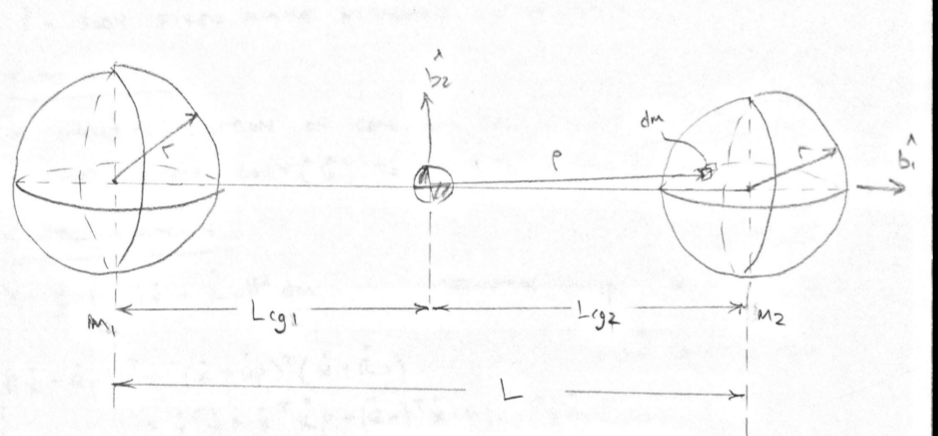
\includegraphics[width=\textwidth]{figures/dumbbell.png}
    \caption{Dumbbell Model of Rigid Spacecraft}
    \label{fig:dumbbell_sc}
\end{figure}
The spacecraft body fixed frame is centered at the center of mass of the vehicle.
The \( \vh{b}_1 \) is axis is aligned with the connecting rod while the \( \vh{b}_2, \vh{b}_3 \) axes span the plane orthogonal to the axis of symmetry of the dumbbell.
The distance from the center of mass to each mass is defined as
\begin{align}\label{eq:dumbbell_mass_distances}
    l_1 &= \frac{m_2}{m_1 + m_2} l, \\
    l_2 &= l - l_1.
\end{align}

\paragraph{Moment of Inertia Derivation}\label{sec:moment_of_inertia}
The inertia tensor/matrix of a rigid body is defined~\cite{greenwood1988} as
\begin{align}
    J_I = \int_{\mathcal{B}} \bracket{ \parenth{\vb{\rho}^T \vb{\rho} }I - \vb{\rho}\vb{\rho}^T} dm, 
\end{align}
where \( \vb{\rho} \in \R^3 \) is the position of a mass element \( dm \) in the body fixed frame of the spacecraft.
One can also use~\cref{eq:xTx} to define the inertia matrix in several other equivalent forms
\begin{align*}
    J_I &= \int_{\mathcal{B}} \bracket{ \parenth{\vb{\rho}^T \vb{\rho} }I - \vb{\rho}\vb{\rho}^T} dm, \\
        &= \int_{\mathcal{B}} \tr{\vb{\rho}\vb{\rho}^T} I - \vb{\rho}\vb{\rho}^T, \\
        &= \int_{\mathcal{B}} \vh{\rho}^T \vh{\rho} dm.
\end{align*}
The location of an infinitesimal mass element \( dm \) can be decomposed into
\begin{align}\label{eq:mass_element_position}
    \vc{\rho}_i = \vc{\zeta} + \vc{\eta}_i, 
\end{align}
where \( \vb{\zeta} \) is the location of the center of \( m_i \) in the spacecraft fixed frame while \( \vc{\eta} \) the position of \( dm \) with respect to the center of \( m_i \) and expressed in the spacecraft fixed frame.
\begin{figure}[htbp]
    \centering
    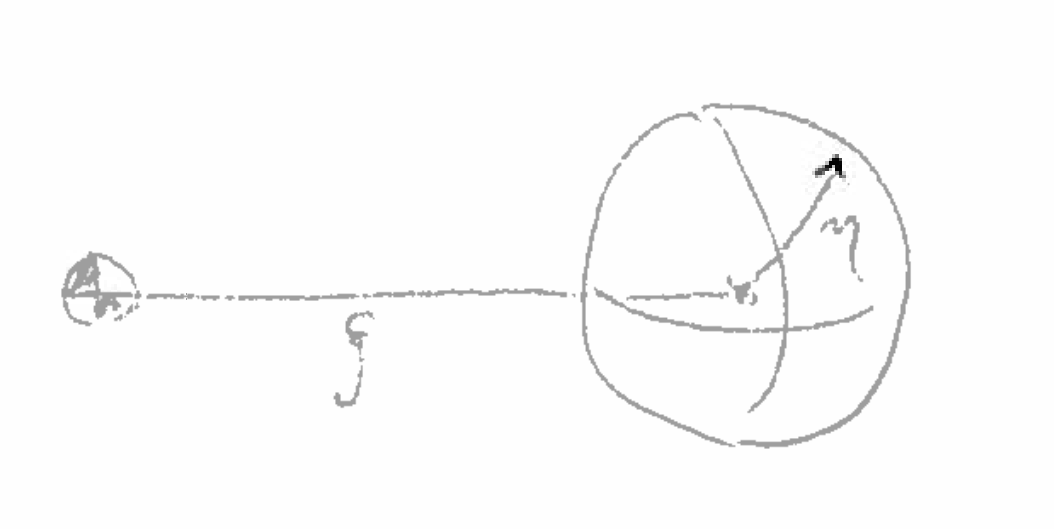
\includegraphics[width=\textwidth]{figures/dumbbell_pos_vector.png}
    \caption{Decomposition of mass element positon vector}
    \label{fig:dumbbell_moi_mass_element_position}
\end{figure}
Using~\cref{eq:mass_element_position} the moment of inertia can be expanded as
\begin{align*}
    J_I &= \sum_i^n \int_{\mathcal{B}_i} \parenth{\vc{\zeta}_i + \vb{\eta}_i}^T \parenth{\vc{\zeta}_i + \vc{\eta}_i } I  - \parenth{\vc{\zeta}_i + \vc{\eta}_i} \parenth{\vc{\zeta}_i + \vc{\eta}_i}^T dm .
\end{align*}
Further expansion leads to
\begin{align*}
    J_I = \sum_i^n \int_{\mathcal{B}_i} \parenth{\vc{\zeta}_i^T \vc{\zeta}_i}I - \vc{\zeta}_i \vc{\zeta}_i^T + \vc{\eta}_i^T \vc{\eta}_i I - \vc{\eta}_i \vc{\eta}_i^T dm, 
\end{align*}
since the cross terms include an integration over the constant density sphere goes to zero:
\begin{align*}
    \int_{\mathcal{B}_i} \vc{\eta}_i dm = 0 .
\end{align*}
The integration is now split into two components: an integration within each sphere, \( \vc{\eta}_i \) terms, and and integration involving the location of the sphere, \( \vc{\zeta}_i \) terms.
As a result, the final moment of inertia of a system of rigid spherical masses is 
\begin{align}\label{eq:dumbbell_moment_of_inertia}
    J_I = \sum_i J_i + m_i \parenth{\vc{\zeta}_i^T \vc{\zeta}_i I - \vc{\zeta}_i \vc{\zeta}_i^T} , 
\end{align}
where \( \vc{\zeta}_i \) is the position of \( m_i \) in the spacecraft fixed frame and the moment of inertia of each sphere is
\begin{align}\label{eq:sphere_moment_of_inertia}
    J_i = \begin{bmatrix} 
        \frac{2}{5} m_i r_i^2 & 0 & 0 \\
        0 & \frac{2}{5} m_i r_i^2 & 0 \\
        0 & 0 & \frac{2}{5} m_i r_i^2 
    \end{bmatrix}.
\end{align}
\Cref{eq:dumbbell_moment_of_inertia} is consitent with the well-known parallel-axis theorem~\cite{greenwood1988}.

%TODO Nonstandard moment of inertia matrix
\paragraph{Nonstandard Moment of Inertia Matrix}
The standard moment of inertia \( J \in \R^{3 \times 3} \) of a rigid body is given by
\begin{align}\label{eq:standard_moment_of_inertia}
    J = \int_{\mathcal{B}} \vh{\rho}^T \vh{\rho} dm 
    = \int_{\mathcal{B}}  
    \begin{bmatrix} 
        y^2 + z^2 & -xy & -zx \\
        -xy & z^2 + x^2 & -yz \\
        -zx & yz & x^2 + y^2
    \end{bmatrix} dm, 
\end{align}
where \( \vc{\rho} = \begin{bmatrix} x & y & z \end{bmatrix}\).
A nonstandard moment of inertia matrix \( J_d \in \R^{3 \times 3 } \) is defined as
\begin{align} \label{eq:nonstandard_moment_of_inertia}
    J_d = \int_{\mathcal{B}} \vc{\rho} \vc{\rho}^T dm = \int_{\mathcal{B}} 
    \begin{bmatrix}
        x^2 & xy & zx \\
        xy & y^2 & yz \\
        zx & yz & z^2
    \end{bmatrix} dm.
\end{align}
Using~\cref{eq:xTx} and the properties of the outer product, it can be shown that
\begin{subequations}\label{eq:moi_transformation}
    \begin{align}
        J &= \tr{J_d} I - J_d, \\
        J_d &= \frac{1}{2} \tr{J} I - J.
    \end{align}
\end{subequations}     
In addition, the following equation is also satisfied for any \( \vc{\Omega} \in \R^3 \)
\begin{align}\label{eq:moi_hat_prop}
    \parenth{J \vc{\Omega}}^\wedge = \vh{\Omega} J_d + J_d \vh{\Omega}.
\end{align}
\Cref{eq:moi_hat_prop} is easy to prove by substituting \( \vc{\Omega} = \begin{bmatrix} \Omega_1 & \Omega_2 & \Omega_3 \end{bmatrix} \) and expanding both sides of~\cref{eq:moi_hat_prop} to
\begin{align*}
    \begin{bmatrix}
        \parenth{J_{yy} + J_{zz}} \Omega_1 - J_{xy} \Omega_2 - J_{zx} \Omega_3 \\
        -J_{xy}\Omega_1 + \parenth{J_{zz} + J_{xx}} \Omega_2 - J_{yz}\Omega_3 \\
        -J_{zx}\Omega_1 - J_{yz}\Omega_2 + \parenth{J_{xx} + J_{yy}} \Omega_3
    \end{bmatrix}^\wedge,
\end{align*}
where \( J_{xy} = \int_{\mathcal{B}} xy dm \in \R \) and the other terms are defined simarily.

\subsection{Inertial Frame Equations of Motion}\label{sec:inertial_dumbbell_eoms}

\paragraph{Kinetic Energy of Dumbbell}\label{sec:inertial_kinetic_energy}
The kinetic energy of the spacecraft begins with the kinematics defined in~\cref{ssec:dumbbell_eoms_reference_frames} as
\begin{align}\label{eq:inertial_KE_1}
    T = \frac{1}{2} \int_{\mathcal{B}} \norm{ \dot{\vc{x}} + \dot{R} \vc{\rho}}^2 dm,
\end{align}
where \( \vc{\rho} \in \R^3 \) defines the position of the mass element \( dm \) in the body fixed frame of the spacecraft.
Expanding the quadratic term in~\cref{eq:inertial_KE_1} results in
\begin{align}\label{eq:inertial_KE_2}
T = \frac{1}{2} \int_{\mathcal{B}}  \norm{\dot{\vc{x}}}^2 + 2 \dot{\vc{x}}^T \dot{R} \vc{\rho} + \norm{\dot{R} \vc{\rho} }^2    dm .
\end{align}
\Cref{eq:inertial_KE_2} is further simplified by noting that
\begin{align*}
    \int_{\mathcal{B}} \vc{\rho} dm = 0,
\end{align*}
and from using the kinematics \( \dot{R} = \R \vh{\Omega} \) for \( \vc{\Omega} \in \R^3 \) 
\begin{align*}
    \norm{\dot{R} \vc{\rho} }^2 &= \vc{\rho}\dot{R}^T \dot{R} \vc{\rho} , \\
                                &=  \vc{\rho}^T \vh{\Omega}^T \vh{\Omega} \vc{\rho} , \\
                                &= \norm{ \vh{\Omega} \vc{\rho} }^2, 
\end{align*}
which results in the following expression for the kinetic energy
\begin{align}\label{eq:inertial_KE_3}
    T = \frac{1}{2} \int_{\mathcal{B}} \braces{ \norm{\dot{\vc{x}}}^2 + \norm{\vh{\Omega} \vc{\rho}}^2 } dm.
\end{align}
The second term \( \norm{\vh{\Omega}\vc{\rho}}^2 \) is simplified to
\begin{align}
    \norm{ \vh{\Omega}\vc{\rho} }^2 &= \parenth{ \vh{\Omega}\vc{\rho}}^T \parenth{\vh{\Omega}\vc{\rho}} , \\
                                    &= \tr{ \vh{\Omega} \vc{\rho} \vc{\rho}^T \vh{\Omega}^T }.
\end{align}
Applying this to~\cref{eq:inertial_KE_3} results in the final form of the kinetic energy as
\begin{align}\label{eq:inertial_kinetic_energy}
    T = \frac{1}{2} m \norm{\dot{\vc{x}}}^2 + \frac{1}{2} \tr{ \vh{\Omega}J_d \vh{\Omega^T } }, 
\end{align}
where we applied the non-standard moment of inertia defined in~\cref{eq:nonstandard_moment_of_inertia}.

\paragraph{Potential Energy of Dumbbell}
The potential energy of the dumbbell is a function of the asteroid potential model.
There are a number of possible models as shown in~\cref{sec:gravitational_models}.
For a rigid body composed of several spherical point masses, the total potential becomes
\begin{align}\label{eq:inertial_potential_energy}
    V(\vc{x}, R, R_A) = \sum_{i}^n - m_i U \parenth{R_A^T \parenth{\vc{x} + R \vc{\rho}_i}},
\end{align}
where \( \vc{x} \in \R^3\) is the position of the center of mass, \( R \in \SO\) is the rotation matrix which transforms vectors from the spacecraft frame to the inertial frame, and \( R_A \in \SO \) is the rotation matrix which transforms vectors from the asteroid frame to the inertial frame.

Using our kinematic variables we can define the kinetic and potential energy of the dumbbell using~\cref{eq:inertial_kinetic_energy,eq:inertial_potential_energy} as
\begin{subequations}\label{eq:dumbbell_kinetic_and_potential_energy}
\begin{align}
    T &= \frac{1}{2} m \norm{\dot{\vb{x}}}^2 + \frac{1}{2} \tr{\vh{\Omega} J_d \vh{\Omega}^T} , \label{eq:dumbbell_kinetic_energy}\\
    V( \vecbf{x}, R ) &=  - m_1 U \parenth{R_A^T \parenth{\vecbf{x} + R \vecbf{\rho}_1}} - m_2 U \parenth{R_A^T \parenth{\vecbf{x} + R \vecbf{\rho}_2}} , \label{eq:dumbbell_potential_energy}
\end{align}
\end{subequations}     
where we utilize the polyhedron potential is defined in~\cref{sec:polyhedron_potential}.
The position of each mass \(m_i\) of the dumbbell is defined in the dumbbell fixed frame by the vector \(\vc{\rho}_i\). 
With~\cref{eq:dumbbell_kinetic_and_potential_energy} one can then use Hamilton's principle to derive the equations of motion.
However, the first step is to determine the varations of \( T, V \).
These variations must be carefully constructed such that the variations of the configuration variables do not violate the nonlinear manifold.
The next step is to define the variations of the kinetic and potential energy to derive the equations of motion, which are given as
\begin{align} 
    \delta T &= \parenth{m_1 + m_2} \ivel^T \delta \dot{\ipos} + \frac{1}{2} \tr{- \dot{\iattvar} \parenth{J \iangvel}^\wedge + \iattvar \parenth{\hat{\iangvel} J \iangvel}^\wedge }, \label{eq:dumbbell_kinetic_energy_variation} \\
    \delta V &= - \sum_{i=1}^2 \braces{ \bracket{m_i \deriv{U}{\apos_i}^T \aatt^T } \delta \ipos +  \tr{\iattvar \parenth{\spos_i \deriv{U}{\apos_i}^T \aatt^T \iatt } }},\label{eq:dumbbell_potential_energy_variation}
\end{align}
where \( \apos_i = \aatt^T \parenth{\ipos + \iatt \spos_i} \) and defines the position of \( m_i \) in the asteroid fixed frame.
The derivation of~\cref{eq:dumbbell_potential_energy_variation,eq:dumbbell_kinetic_energy_variation} is provided in~\cref{proof:inertial_dumbbell_eoms}.

Using the variations of the kinetic and potential energy we can derive the equations of motion of the dumbbell spacecraft about an asteroid using Hamilton's principle. 
Hamilton's principle states that the variation of the action integral
\begin{align}\label{eq:action_integral}
    \mathcal{G} = \int_{t_0}^{t_f} T(\dot{\vc{q}}) - V(\vc{q}) dt,
\end{align}
is stationary with for all possible variations with fixed endpoints. 
In other words, 
\begin{align}\label{eq:hamiltons_principle}
    \delta \mathcal{G}  = \int_{t_0}^{t_f} \delta T - \delta V dt = 0.
\end{align}
Following the derivation presented in~\cref{proof:inertial_dumbbell_eoms} gives the inerital equations of motion in Lagrangian form as
\begin{align}
    \dot{\ipos} &= \ivel, \label{eq:inertial_position_dynamics}\\
    \parenth{m_1 + m_2} \dot{\ivel} &= - \sum_{i=0}^2 m_i \aatt \deriv{U}{\apos_i} + u_f, \label{eq:inertial_velocity_dynamics}\\
    \dot{\iatt} &= \iatt \iangvel, \label{eq:inertial_attitude_dynamics}\\
    J \dot{\iangvel} + \hat{\iangvel} J \iangvel &= \sum_{i=0}^2 m_i \hat{\spos}_i \iatt^T \aatt \deriv{U}{\apos_i} + u_m. \label{eq:inertial_angvel_dynamics}
\end{align}
The vectors \( \apos_i \) define the position of the dumbbell mass \( m_i \) in the asteroid fixed frame
\begin{align}
    \apos_i &= \aatt^T \parenth{\ipos + \iatt \spos_i},
\end{align}
where \( \spos_i \) defines the position of each mass in the spacecraft fixed body frame.
The control inputs to the spacecraft are defined by \( u_f, u_m \in \R^3 \) which define the control force represented in the inertial frame and the control moment represented in the spacecraft frame, respectively. 
% TODO Ensure that \eta is not bold (it's a matrix) also all vectors should be bold and lower case

\paragraph{Inertial Equations of motion: Hamiltonian Form}\label{sec:inertial_hamiltonian_form}
% TODO Check hte legendre transformation is correct
Hamilton's equations allows for the representation of the second order equations derived using the Euler-Lagrange equation as a system of \( 2n \) first order equations called a hamiltonian system of equations or canonical equations~\cite{arnold1989}.
Hamilton's equations are derivable direclty from the Lagrangian through the use of the Legendre transformation which is a mapping \( \left( q, \dot{q},t\right) \rightarrow \left(q, p, t \right) \) where \( p_i\) is the generalized momenta,
\begin{align}\label{eq:legendre_transform}
	p_i = \deriv{L}{\dot{q}}
\end{align}
The Legendre transformation is useful for variational equations
\begin{align*}
	df &= u dx + v dy \\
\end{align*}
where
\begin{align*}
	u &= \deriv{f}{x} \quad v &= \deriv{f}{y}
\end{align*}
To change from \( \left( x, y\right) \rightarrow \left(u,y \right) \)
\begin{align*}
	g &= f - u x\\
	dg &= df - u dx - x du\\
	dg &= v dy - x du \\
	x&= -\deriv{g}{u} \\
    v&= \deriv{g}{y}
\end{align*}

In the continuous time case, one can define the Hamiltonian in terms of the Lagrangian as
\begin{align}\label{eq:hamiltonian}
	H &= \sum_{i = 1}^N p_i \dot{q}_i - L \left( q_i,\dot{q}_i, t \right)
\end{align}
Applying~\cref{eq:legendre_transform} and taking the variation of~\cref{eq:hamiltonian} allows us to derive the equations of motion in Hamiltonian form
\begin{align}\label{eq:hamilton_eq}
	\dot{q}_i &= \deriv{H}{p_i} \\
	\dot{p}_i &= - \deriv{H}{q_i} + Q_i \\
	\deriv{L}{t} &= -\deriv{H}{t}
\end{align}
Again we are left with \( 2n \) first order differential equations that describe the system dynamics in terms of the generalized position and momenta \( q_i \) and \( p_i\), respectively.
For the inertial equations of motion, we define the linear and angular momentum of the spacecraft as \( \ilinmom \in \R^3\) and \( \iangmom \in \R^3 \), respectively.
The system momenta is related to the velocities by the transformations
\begin{align}
    \ilinmom &= \parenth{m_1 + m_2} \ivel , \\
    \iangmom & = J \iangvel.
\end{align}

\subsection{Asteroid Frame Equations of Motion}
The complete motion of rigid bodies under the influence of their mutual gravity only depends on the relative position and relative attitude of the bodies~\cite{lee2007a}.
This is a consequence of the fact that the gravitational potential can be described using only the relative position.
Physically, this is due to the fact that the total linear and angular momentum of the system is conserved.
In astrodynamics, this fact is typically used to reduce the two body problem to that of the relative two body problem which affords convienent analytical solutions~\cite{vallado2007,bate1971}.
In this section, the equations of motion of a rigid spacecraft are derived in the asteroid fixed frame.
This derivation can be considered a specific example of the relative full body problem and is readily generalized to multiple bodies~\cite{lee2007a}.

The relative motion of a dumbbell spacecraft with respect to an asteroid are defined by the kinematics:
\begin{align}
    \gls{sym:rpos} &= R_A^T \vc{x}, \label{eq:relative_position} \\
    \gls{sym:rvel} &= R_A^T \dot{\vc{x}}, \label{eq:relative_velocity},
\end{align}
where \( \gls{sym:rpos} \in \R^3 \) is the relative position of the spacecraft with respect to the asteroid and expressed in the asteroid fixed frame, and \( \gls{sym:rvel} \in \R^3 \) is the relative velocity of the spacecraft with respect to the asteroid and expressed in the asteroid fixed frame.
The relative attitude kinematics are defined by
\begin{align}
    \gls{sym:ratt} &= R_A^T R, \label{eq:relative_attitude} \\
    \gls{sym:rangvel} &= \gls{sym:ratt} \vc{\Omega}, \label{eq:relative_angular_velocity}
\end{align}
where \( \gls{sym:ratt} \in \SO \) is the relative attitude of the spacecraft with respect to the asteroid.
\( \gls{sym:ratt} \) transforms vectors from the spacecraft fixed frame to the asteroid fixedf frame.
\( \gls{sym:rangvel} \in \R^3 \) is the angular velocity of the spacecraft with respect to the inertial frame and expressed in the inertial frame.

As in~\cref{sec:inertial_dumbbell_eoms}, we first seek to define the kinetic and potential energy of the dumbbell in terms of these relative kinematics. 
Afterwards, the variations are taken to derive the equations of motion.
In this analysis, it is assumed that the motion of the asteroid is not impacted by that of the dumbbell.
In other words, the size of the dumbbell spacecraft is significantly less than that of the dumbbell. 
As a result, the motion of the asteroid is unaffected by that of the spacecraft.

The kinetic energy defined in the inertial frame is given by~\cref{eq:inertial_kinetic_energy} and is transformed using~\cref{eq:relative_position,eq:relative_angular_velocity} as
\begin{align}\label{eq:relative_kinetic_energy_1}
    T &= \frac{1}{2} \parenth{m_1 + m_2} \parenth{\gls{sym:rvel} \gls{sym:Ra}[^T] \gls{sym:Ra} \gls{sym:rvel}} + \frac{1}{2} \tr{\parenth{\gls{sym:ratt}[^T] \gls{sym:rangvel}}^\wedge J_d \parenth{\gls{sym:ratt}[^T] \gls{sym:rangvel} }^{\wedge T}}. 
\end{align}
Using~\cref{eq:hatRxR,eq:trABC} in~\cref{eq:relative_kinetic_energy_1} results in
\begin{align}\label{eq:relative_kinetic_energy_2}
    T = \frac{1}{2} \parenth{m_1 + m_2} \norm{\gls{sym:rvel}}^2 + \frac{1}{2} \tr{\hat{\gls{sym:rangvel}} \gls{sym:ratt} J_d \gls{sym:ratt}[^T] \hat{\glsentrytext{sym:rangvel}}^T}.
\end{align}
The term \( \gls{sym:ratt} J_d \gls{sym:ratt}[^T] = J_{d_R}\) is the expression of the nonstandard moment of inertia tensor of the dumbbell expressed in the asteroid fixed frame. 
It is now a time varying inertia matrix as the relative attitude \( \gls{sym:ratt} \) is a function of time.
Using~\cref{eq:hatRxR} it can be shown that \( J_{d_R} \) also satisfies a similar property as~\cref{eq:moi_hat_prop}, 
\begin{align}\label{eq:moi_relative_hat_prop}
    \parenth{J_R \gls{sym:rangvel}}^\wedge = \hat{\gls{sym:rangvel}} J_{d_R} + J_{d_R}\hat{\gls{sym:rangvel}},
\end{align}
where \( J_R = \gls{sym:ratt} J \gls{sym:ratt}[^T] \in \R^{3 \times 3}\) is the standard moment of inertia matrix of the spacecraft expressed with respect to the asteroid fixed frame.
Using this definition the relative kinetic energy is given as
\begin{align}\label{eq:relative_kinetic_energy}
    T &= \frac{1}{2} \parenth{m_1 + m_2} \norm{\gls{sym:rvel}}^2 + \frac{1}{2} \tr{\hat{\gls{sym:rangvel}} J_{d_R} \hat{\glsentrytext{sym:rangvel}}^T}.
\end{align}

The potential energy is already defined in terms of the relative position of the dumbbell with respect to the asteroid.
Using the relative kinematics given in~\cref{eq:relative_position,eq:relative_attitude} gives
\begin{align}\label{eq:relative_potential_energy}
    V = -m_1 U( \gls{sym:rpos} + \gls{sym:ratt} \vc{\rho}_1) - m_2 U(\gls{sym:rpos} + \gls{sym:ratt} \vc{\rho}_2).
\end{align}
Using~\cref{eq:relative_kinetic_energy,eq:relative_potential_energy}, the reduced Langrangian is expressed in terms of the relative kinematics as 
\begin{align}\label{eq:relative_lagrangian}
    L = T-V =& \frac{1}{2} \parenth{m_1 + m_2} \norm{\gls{sym:rvel}}^2 + \frac{1}{2} \tr{\hat{\gls{sym:rangvel}} J_{d_R} \hat{\glsentrytext{sym:rangvel}}^T} \nonumber \\
             &+m_1 U(\gls{sym:rpos} + \gls{sym:ratt} \vc{\rho}_1) + m_2 U(\gls{sym:rpos} + \gls{sym:ratt} \vc{\rho}_2) .
\end{align}

\subsection{Variation of relative Lagrangian}\label{ssec:var_rel_lagrangian}

In a process similar to~\cref{sec:inertial_dumbbell_eoms} we use Hamilton's principle to derive the relative equations of motion, in the asteroid fixed frame, by finding the variation of~\cref{eq:relative_lagrangian}.
Ensuring that the action integral is stationary for all possible variations leads to the equations of motion.
A key difference is that the variations of the relative variables must be careful chosen to respect the geometry of the configuration manifold.
Furthermore, the relative variations must also obey the constraints of the inertial variations.
The derivation of the variation of the relative Lagrangian is shown in~\cref{proof:relative_dumbbell_eoms}.


The variation of the reduced potential energy, shown in~\cref{eq:relative_potential}, is given by
\begin{align}\label{eq:relative_potential_variation_1}
    \delta U &= -m_1 \deriv{U}{\vecbf{z}_1} \delta \vecbf{z}_1 - m_2 \deriv{U}{\vecbf{z}_2} \delta \vecbf{z}_2 ,
\end{align}
where \( \delta \vecbf{z}_1 \) and \( \delta \vecbf{z}_2\) are defined similar to those used in~\cref{sec:inertial_eoms} as 
\begin{align}\label{eq:relative_z}
    \delta \vecbf{z}_1 &= \delta \vecbf{\chi} + \delta R \vecbf{\rho}_1 , \\
    \delta \vecbf{z}_2 &= \delta \vecbf{\chi} + \delta R \vecbf{\rho}_2 .
\end{align}
Substituting~\cref{eq:relative_z} into~\cref{eq:relative_potential_variation_1} and simplifying gives
\begin{align}\label{eq:relative_potential_varation}
    \delta U &= -m_1 \deriv{U}{\vecbf{z}_1}^T \vecbf{\chi} - m_2 \deriv{U}{\vecbf{z}_2} \vecbf{\chi} - m_1 \tr{\eta R \deriv{U}{\vecbf{z}_1} \vecbf{\rho}_1^T} - m_2 \tr{\eta R \deriv{U}{\vecbf{z}_2} \vecbf{\rho}_2^T} .
\end{align}

Combining~\cref{eq:relative_potential_varation,eq:relative_kinetic_variation} in the variation of the action integral is given by
\begin{align}\label{eq:relative_variation_action_integral}
    \delta I =& \int_{t_1}^{t_2} \parenth{m_1 + m_2} \delta \vecbf{V} \parenth{\dot{\vecbf{\chi}} + S(\vecbf{\Omega}_A) \vecbf{\chi}} + \frac{1}{2} \tr{- \dot{\eta} S(J_R \vecbf{\Omega}) + \eta S(\vecbf{\Omega}_A \times J_R \vecbf{\Omega})} \nonumber\\
    &+m_1 \deriv{U}{\vecbf{z}_1}^T \vecbf{\chi} + m_2 \deriv{U}{\vecbf{z}_2} \vecbf{\chi} + m_1 \tr{\eta R \deriv{U}{\vecbf{z}_1} \vecbf{\rho}_1^T} + m_2 \tr{\eta R \deriv{U}{\vecbf{z}_2} \vecbf{\rho}_2^T} \, dt , \nonumber\\
    =& \int_{t_1}^{t_2} \parenth{m_1 + m_2} \dot{\vecbf{V}}^T \vecbf{\chi} + \parenth{m_1 + m_2} \vecbf{V}^T S(\vecbf{\Omega}_A) \vecbf{\chi} \nonumber \\
    &+ \frac{1}{2} \tr{\eta \braces{S(\dot{J_R \vecbf{\Omega}}) + S(\vecbf{\Omega}_A \times J_R \vecbf{\Omega})}} + m_1 \deriv{U}{\vecbf{z}_1}^T \vecbf{\chi} + m_2 \deriv{U}{\vecbf{z}_2}^T \vecbf{\chi} \nonumber\\
    &+ m_1 \tr{\eta R \deriv{U}{\vecbf{z}_1} \vecbf{\rho}_1^T} m_2 \tr{\eta R \deriv{U}{\vecbf{z}_2} \vecbf{\rho}_2^T} \, dt ,
\end{align}
where we used integration by parts to simplify integral
\begin{align*}
    \int \parenth{m_1 + m_2} \vecbf{V}^T \dot{\vecbf{\chi}} \, dt &= \left. \parenth{m_1 + m_2 } \vecbf{\chi} \right|_{t_0}^{t_f} - \int \parenth{m_1 +m_2} \dot{\vecbf{V}}^T \vecbf{\chi} \, dt , \\
    \int \frac{1}{2} \tr{- \dot{\eta} S(J_R \vecbf{\Omega}) + \eta S(\vecbf{\Omega}_A \times J_R \vecbf{\Omega})} &= \left. \frac{1}{2} \tr{-\eta S(J_R \vecbf{\Omega})} \right|_{t_0}^{t_f} - \int \frac{1}{2} \tr{-\eta S(\dot{J_R \vecbf{\Omega}})} \, dt.
\end{align*}
Since~\cref{eq:relative_variation_action_integral} must be zero for all admissable variations the  equations of motion are given by
\begin{align}\label{eq:relative_eoms}
    \parenth{m_1 +m_2} \dot{\vecbf{V}} + \parenth{m_1 + m_2} S(\vecbf{\Omega}_A) \vecbf{V} &= m_1 \deriv{U}{\vecbf{z}_1} + m_2 \deriv{U}{\vecbf{z}_2} , \\
    S(\dot{J_R \vecbf{\Omega}}) + S(\vecbf{\Omega}_A \times J_R \vecbf{\Omega}) &= m_1 \vecbf{\rho}_1 \deriv{U}{\vecbf{z}_1}^T R^T - m_1 R \deriv{U}{\vecbf{z}_1} \vecbf{\rho}_1^T + m_2 \vecbf{\rho}_2 \deriv{U}{\vecbf{z}_2} R^T - m_2 R \deriv{U}{\vecbf{z}_2} \vecbf{\rho}_2^T .
\end{align}
Using a similar process as~\cref{sec:inertial_eoms} we can redefine the external moment due to gravity as
\begin{align}
    M_1 &= m_1 \parenth{\vecbf{r}_1 \times \vecbf{u}_1 + \vecbf{r}_2 \times \vecbf{u}_2 + \vecbf{r}_3 \times \vecbf{u}_3} , \\
    M_2 &= m_1 \parenth{\vecbf{r}_\alpha \times \vecbf{u}_\alpha + \vecbf{r}_\beta \times \vecbf{u}_\beta + \vecbf{r}_\gamma \times \vecbf{u}_\gamma} , 
\end{align}
where the vectors \( \vecbf{r}_i \) and \( \vecbf{u}_i \) are defined as
\begin{align*}
    R = \begin{bmatrix} \vecbf{r}_1 \\ \vecbf{r}_2 \\ \vecbf{r}_3 \end{bmatrix} = \begin{bmatrix} \vecbf{r}_\alpha \\ \vecbf{r}_\beta \\ \vecbf{r}_\gamma \end{bmatrix} \quad
    \vecbf{\rho}_1 \deriv{U}{\vecbf{z}_1}^T = \begin{bmatrix} \vecbf{u}_1 \\ \vecbf{u}_2 \\ \vecbf{u}_3 \end{bmatrix}, \vecbf{\rho}_2 \deriv{U}{\vecbf{z}_2}^T = \begin{bmatrix} \vecbf{u}_\alpha \\ \vecbf{u}_\beta \\ \vecbf{u}_\gamma \end{bmatrix} .
\end{align*}
The time derivative \( \dot{J_R}\) is computed from
\begin{align*}
    \dot{J}_R &= \dot{R} J_1 R^T + R J_1 \dot{R}^T , \\
    &= \parenth{S(\vecbf{\Omega})R - S(\vecbf{\Omega}_2) R)} J_1 R^T + R J_1 \parenth{R^T S(\vecbf{\Omega}_2 - R^T S(\vecbf{\Omega}) } \\
    &= S(\vecbf{\Omega}) R J_1 R^T - S(\vecbf{\Omega}_2) R J_1 R^T + R J_1 R^T S(\vecbf{\Omega}_2) - R J_1 R^T S(\vecbf{\Omega}) \\
    &=  \parenth{S(\vecbf{\Omega}) - S(\vecbf{\Omega}_2)} R J_1 R^T + R J_1 R^T \parenth{S(\vecbf{\Omega}_2) - S(\vecbf{\Omega})} .
\end{align*}
Using this relatipnship the term \( \dot{\parenth{J_R \vecbf{\Omega}}}\) is given by
\begin{align*}
    \dot{\parenth{J_R \vecbf{\Omega}}} &= \dot{J}_R \vecbf{\Omega} + J_R \dot{\vecbf{\Omega}} \\
    &= \bracket{\parenth{S(\vecbf{\Omega}) - S(\vecbf{\Omega}_2)} R J_1 R^T + R J_1 R^T \parenth{S(\vecbf{\Omega}_2) - S(\vecbf{\Omega})}} \vecbf{\Omega} + J_R \dot{\vecbf{\Omega}} .
\end{align*}
In summary, the relative equations of motion are given as
\begin{align}
    \dot{\vecbf{\chi}} + \vecbf{\Omega}_A \times \vecbf{\chi} &= \vecbf{V} ,\\
    \dot{R} &= S(\vecbf{\Omega}) R - S(\vecbf{\Omega}_A ) R , \\
    J_R \dot{\Omega} &= M_1 + M_2 - \vecbf{\Omega}_A \times J_R \vecbf{\Omega} -\bracket{\parenth{S(\vecbf{\Omega}) - S(\vecbf{\Omega}_2)} R J_1 R^T + R J_1 R^T \parenth{S(\vecbf{\Omega}_2) - S(\vecbf{\Omega})}} \vecbf{\Omega} , \\
    \parenth{m_1 + m_2} \dot{\vecbf{V}} &= m_1 \deriv{U}{\vecbf{z}_1} + m_2 \deriv{U}{\vecbf{z}_2} - \parenth{m_1 +m_2} S(\vecbf{\Omega}_A) \vecbf{V} .
\end{align}

\section{Gravitational Models around Small-Bodies}\label{sec:gravitational_models}
Due to the irregular shape of small-bodies, the gravitational field around these bodies is equally irregular.
Furthermore, the relative size of the spacecraft in comparison with the orbital radius and small-body creates a much larger coupling between the translational and rotational states of the spacecraft.
In addition, spacecraft will tend to operate in very close proximity to the surface.
As a result, accurate computation of the gravitational field around these irregular bodies is critical to safe and effective operations.
The classic approach to determining the gravitational force is to apply Newton's law of Universal gravitation.
The force due to gravity between two point masses is defined as
\begin{align}\label{eq:newton_universal_gravitation}
    \vb{F}_g =  - G \frac{m_1 m_2}{r^2} \frac{\vb{r}}{r},
\end{align}
where \( G \) is the universal gravitational constant, \( \vb{r} \) is the relative position vector between the points of mass \( m_1, m_2\), respectively.

\begin{figure}
    \centering
    \includegraphics[width=\textwidth]{example-image-golden}
    \caption{Newton's Law of Unviversal Gravitation~\label{fig:universal_gravity}}
\end{figure}

This gravitational model is defined if point masses or bodies which can be modeled as point masses, such as spherically symmetric planets.
However, it is not possible to model an irregular asteroid, or an orbiting spacecraft, as point masses.
Instead, one must treat both bodies as extended objects and compute the gravitational force from the potential function as an integral over the entire body, \( \mathcal{B}\),
\begin{align}\label{eq:volume_integral_potential}
\vb{F}_g ( \vb{r}) = \nabla U = G \int_{\mathcal{B}} \frac{1}{\norm{\vb{r} - \vb{\rho} }} dm (\vb{\rho}),
\end{align}
where \( \vb{r} \) is the position of the field point, \( \vb{\rho} \) is the position of the differential mass element of the body and \( \nabla U \) is defined as the gradient of \( U \) with respect to the standard cartesian basis vectors
\begin{align*}
    \nabla = \deriv{}{x} \hat{\vb{i}} + \deriv{}{y} \hat{\vb{j}} + \deriv{}{z} \hat{\vb{k}}.
\end{align*}

The first approach, sometimes termed the \textit{mass-concentration}, or \textit{mascon} method, approximates the integral using an infinite sum of point masses \( m_i\) located at \( \vb{r}_i \).
The potential on our object of interest then becomes the summation of the potential caused by each mass \( m_i \) as shown in~\cref{eq:mass_con_potential}.
\begin{align}\label{eq:mass_con_potential}
    U = G \sum_{i=0}^{\infty} \frac{m_i}{\norm{\vb{r} - \vb{\rho}_i}}
\end{align}
The method distributes a colleciton of point masses uniformly throughout the body such that the total mass is equal to the body.
While conceptually simple, and relatively straight forward to numerically implement, the mascon approach has several drawbacks~\cite{scheeres2012a}.
First, the mascon approach does not provide any method to determine if the object of interest is inside or outside of the body.
As a result, any numerical simulation making use of the mascon approach will require a secondary operation to determine if the spacecraft has collided with the surface.
Additionaly, it has been shown that the mascon approach is more computationaly demanding than other methods, namely the spherical harmonic or polyhedron potential method~\cite{werner1996}.
Finally, while the mascon method will provide the true gravity field in the limit as the number of invidual point masses becomes large, there are significant errors in the direction of the force vector~\cite{werner1996}.

It can be shown that the gravitational potential will satisfy Laplace's equation outside of the body
\begin{align}
    \nabla^2 U = 0
\end{align}
and Poisson's equation inside of the body
\begin{align}
    \nabla^2 U = - 4 \pi G \sigma
\end{align}
where \( \sigma \) is the local density of the body.
Laplace's equation can be solved using a seperation of variables in terms of spherical coordinates~\cite{scheeres2012a}.
The transformation between cartesian, \( \vb{r} = x \hat{\vb{x}} + y \hat{\vb{y}} + z \hat{\vb{z}}\),  and spherical coordinates, is given by
\begin{subequations}
    \begin{align*}
        r &= \sqrt{x^2 + y^2 + z^2}, \\
        \sin \phi &= \frac{z}{r}, \\
        \tan \lambda &= \frac{y}{x},
    \end{align*}
\end{subequations}
where \( \phi \) is the latitude and \( \lambda\) is the longitude.
One can then follow a standard derivation~\cite{vallado2007} to arrive at a general form of the spherical harmonic potential model:
\begin{align}\label{eq:spherical_harmonic}
    U = \frac{\mu}{r} \sum_{l=0}^\infty \sum_{m=0}^l \parenth{\frac{r_o}{r}}^n P_{l, m}(\sin \phi) \braces{ C_{lm} \cos(m \lambda) + S_{lm} \sin(m \lambda)},
\end{align}
where \( \mu = G M \) is the gravitational parameter of the body, \( r_o\) is a normalizing radius, which is typically chosen as the mean or maximum radius of the attracting body.
The term \( P_{l, m} \) are the associated Legendre functions while \( C_{lm}\) and \( S_{lm}\) are called the spherical harmonic coefficients or Stoke's coefficients. 
The Legendre functions are given in closed form by~\cite{scheeres2012}
\begin{subequations}
\begin{align}
    P_{l, m} \parenth{ \sin \delta} &= \cos^m \phi \sum_{i = 0}^{\text{int}\bracket{l - \frac{m}{2}}} T_{lmi} \sin^{l - m - 2i} \phi ,  \\
T_{lmi} &= \frac{\parenth{-1}^i\parenth{2l - 2i}!}{2^l i! \parenth{l - i}!\parenth{l - m- 2i}!}.
\end{align}
\end{subequations}
where \( \text{int}\bracket{x}\) defines the integer portion of \( x \).
Defining the spherical harmonic coefficients, namely \( C_{lm}, S_{lm}\), is equivalent to defining the mass distribution of the body.
The spherical harmonic coefficients have been determined for many planetary bodies, such as the Earth, to a very high fidelity~\cite{vallado2007,pavlis2012}.

% TODO Continue with the drawbacks of spherical harmonic
The spherical harmonic gravity model is not applicable in all situations.
A implicit assumption of the spherical harmonic expansion are that the series converge to the true gravitational field.
It can be shown that the expansion will diverge when applied to a point within the maximum circumscribing sphere of the body~\cite{scheeres2012a}.
A typical remedy is to derive two different expansions, the first:
\begin{align}
    U = \frac{1}{V} \int_{\mathcal{B}} \parenth{ \frac{\rho}{r}}^i P_{i0} \parenth{ \frac{\vb{r} \cdot \vb{\rho}}{ r \rho}} dV, 
\end{align}
is only valid when \( \norm{\rho} < r \) and is not defined at \( \norm{\vb{\rho}} = r\).
A second expansion can be derived for the case \(\norm{\vb{\rho}} > r \) as
\begin{align}
    U = \frac{1}{V} \int_{\mathcal{B}} \parenth{ \frac{r}{\rho}}^i P_{i0} \parenth{ \frac{\vb{r} \cdot \vb{\rho}}{ r \rho}} dV. 
\end{align}
If a finite density is assumed, then the gravitational field will vanish at \( \norm{\vb{\rho}} = r \).
As a result of this discontinuity, the expansion coefficients become a function of the radius of the body and must be recomputed as the body changes.
These limitations mean that in practice the spherical harmonic expansion model cannot be used for the gravity model when operating around an irregular body.
The divergence of the expansion causes the gravitational field to become meaningless when close to the surface and make the use of the spherical harmonic model worthless for dynamic computations.

% TODO Add picture of biroullion sphere
% TODO Add glossary entry for biroullion sphere
% TODO Show picture of point masses and newton's law and add near the equation
% TODO Add picture of MASCON model (many point masses)

An alternative approach is based on using a specified shape of the body to determine a closed form solution to the gravitational potential.
Each of these methods are based on a known shape of the body and a strong assumption on the density variation, frequently assuming a homegenous body with constant density.
The simplest solution is based on a spherical body with a radially-varying density distribution.
This type of model is best applicable for centrobaric bodies, such as the Earth and many planetary bodies.
% TODO Write down the spherical potential for a radially varying distribution from AAE532
The solutions for the constant density ellipsoid and constant density polyhedron are more useful for operations near small irregular bodies.
These methods provide exact, closed-form solutions which are valid up to the surface of the body and have been used in the majority of research near the surface of small bodies.
Here we present the ellipsoid and polyhedron potential models which are commonly used heavily used in research around small bodies.

\subsection{Constant Density Ellipsoid}\label{sec:constant_density_ellipsoid}

% TODO Need to add citations for these statements
The ellipsoid gravitational model assumes that the small body is accurately represented by a constant density ellipsoid.
This strong assumption is appropriate for many bodies as they are relatively close to ellipsoidal in shape.
Furthermore, many asteroids are also well represented with a constant density. 
In addition, based on ground measurements alone it is frequently not possible to arrive at a more accurate shape beyond that of a triaxial ellipsoid.
The triaxial ellipsoid has semi-major axes \( \gamma \leq \beta \leq \alpha\) and the surface of the body is defined by the implicit equation
\begin{align}
    \parenth{\frac{x}{\alpha}}^2 + \parenth{\frac{y}{\beta}}^2 + \parenth{\frac{z}{\gamma}}^2 \leq 1 . 
\end{align}
% TODO Draw a picture of ellipsoid with teh axes labeled
\begin{figure}
    \centering
    \includegraphics[width=\textwidth]{example-image-golden}
    \caption[Triaxial Ellipsoid]{Constant Density Tri-Axial Ellipsoid Model~\label{fig:triaxial_ellipsoid}}
\end{figure}
Using this model, the gravitational potential outside the body is given by
\begin{subequations}
\begin{align}
    U (\vb{r}) &= - \frac{3 \mu}{4} \int_{\lambda{\vb{r}}}^{\infty} \frac{\phi ( \vb{r},  u) }{ \Delta(u)} du, \\
    \phi(\vb{r}, u) &= \frac{x^2}{\alpha^2 + u} + \frac{y^2}{\beta^2 + u} + \frac{z^2}{\gamma^2 + u} - 1 , \\
    \Delta(u) &= \sqrt{\parenth{\alpha^2 + u} \parenth{\beta^2 + u} \parenth{\gamma^2 + u}},
\end{align}
where \( \lambda(\vb{r}) \) is defined by \( \phi(\vb{r}, \lambda) = 0 \).
The position vector should be transformed into the principle axis frame, such that the \( \hat{\vb{x}} \) axis is aligned along the long axis \( \alpha \), \( \hat{\vb{y}} \) is aligned with the intermediate axis \( \beta \), and \( \hat{\vb{z}} \) is aligned along the short axis \( \gamma \).
A straightforward application of Leibniz's rule allows one to compute the Jacobian and Hessian of \( U \)~\cite{scheeres2012a}.
\end{subequations}  

The constant density ellipsoid model provides a closed form solution for the gravitational potential but suffers from a number of disadvantages.
It is based on a specific body shape, namely the triaxial ellipsoid, and is not applicable for bodies that have a different shape.
Approximating the shape of many small bodies as triaxial ellipsoids is appropriate for many first order dynamical simulations and analysis.
Insight into the dynamic environment~\cite{guelman2014}, periodic orbits~\cite{hu2002}, equilibrium points~\cite{scheeres1994}, or surface dynamics~\cite{furfaro2013} are all greatly simplified with use of the ellipsoid shape approximation.
However, once additional data is received, such as improved ground imaging or in-situ measurements from a spacecraft, the shape model of the small body will become more accurate and cause it to diverge from the ellipsoid assumption.
At this point, the dynamic model is no longer valid and must be modified for use with the updated shape data.
In the case of an operational mission, this may require extensive redevelopment of core flight software and the associated testing to ensure it is functioning properly. 
Furthermore, the model is defined in terms of continuous integrals which must be numerically evaluated using methods of Carlson's elliptic integrals.
Due to these reasons, we instead model the gravitational potential using the polyhedron potential model which alleviates many of these issues.

\subsection{Polyhedron Potential Model}\label{sec:polyhedron_potential}

% TODO Intro to the potnetial model. Cite some papers. Discuss the benefits
Robert Werner developed the polyhedron potential model in a series of papers in the mid-1990s~\cite{werner1994,werner1996,werner1997}.
The method provides a closed form solution for the gravitational potential about any arbitrary constant density polyhedron.
While the solution is closed form, the implementation requires efficient software to compute the potential as it is dependent on a summation over all faces and edges of the polyhedron.
There is no requirement on the polyhedron shape and it can incorporate craters, ridges, or even holes through the small body.
Furthermore, the accuracy of the model is solely dependent on the fidelity of the shape in representing the true body and the constant density assumption.
For bodies with varying density, it is possible to augument the polyhedron potential model to account for the density variations~\cite{scheeres2000a}.
This approach alleviates the divergence issue of the spherical harmonic model and is applicable for all points on or above the surface and is ideal for general operations around small bodies.
The polyhedron potential model has become the defacto standard for small body missions and has been used operationally.
In this section we summarize the polyhedron potential model based on the derivations of Werner.
We additionally present some of the implementation details in our model and the adaptions for use with the \texttt{Surface\_mesh} data structure presented  in~\cref{sec:polyhedron_data_structures}.

% TODO Add a link to the section that talks about polyhedrons
This model is composed of a polyhedron, which is a three-dimensional solid body, that is defined by a series of vectors in the asteroid fixed frame.
The vectors define vertices in the asteroid fixed frame and combinations of these vertices then define planar faces which compose the surface of the asteroid.
Additionally, we assume that each face is a triangle composed of three vertices and three edges.
As a result, only two faces meet at each edge while three faces meet at each vertex.
Only the body-fixed vectors, and their associated topology, is required to define the exterior gravitational model.

% TODO Need a picture of the edges/faces/halfedges
Consider three vectors \( \vecbf{v}_1, \vecbf{v}_2, \vecbf{v}_3 \in \R^{3 \times 1} \), assumed to be ordered in a counterclockwise direction about an outward facing normal vector, which define a face.
It is easy to define the three halfedges of each face as
\begin{align}\label{eq:edges}
    \vecbf{h}_{i} = \vecbf{v}_{i+1} - \vecbf{v}_i \in \R^{3 \times 1 },
\end{align}
where the index \( i \in \parenth{1,2,3} \) is used to permute all vertices of each face.
Each halfedge has an opposing or inverse which is a member of the adjacent face and orientated in the opposite direction.
We can also define the outward normal vector to each face \( f \) as
\begin{align}\label{eq:face_normal}
    \hat{\vecbf{n}}_f &= \parenth{\vb{h}_2} \times \parenth{\vb{h}_1} \in \R^{3 \times 1},
\end{align}
and the outward facing normal vector to each halfedge as
\begin{align}\label{eq:edge_normal}
    \hat{\vecbf{n}}_{i}^f &= - \parenth{\vb{h}_i} \times \hat{\vecbf{n}}_f \in \R^{3 \times 1}.
\end{align}
For each face, we define the face dyad \( \vecbf{F}_f \) as
\begin{align}\label{eq:face_dyad}
    \vecbf{F}_f &= \hat{\vecbf{n}}_f \hat{\vecbf{n}}_f \in \R^{3 \times 3}.
\end{align}
Each edge is a member of two faces and has an outward pointing edge normal vector, given in~\cref{eq:edge_normal}, perpendicular to both the edge and the face normal.
For the edge connecting the vectors \( \vecbf{v}_1 \) and \( \vecbf{v}_2 \), which are shared between the faces \(A\) and \( B\), the per edge dyad is given by
\begin{align}\label{eq:edge_dyad}
    \vecbf{E}_{12} = \hat{\vecbf{n}}_A \hat{\vecbf{n}}_{12}^A + \hat{\vecbf{n}}_B \hat{\vecbf{n}}_{21}^B \in \R^{3 \times 3}.
\end{align}
The edge dyad \( \vecbf{E}_e  \), is defined for each edge and is a function of the two adjacent faces meeting at that edge.
The face dyad \( \vecbf{F}_f \), is defined for each face and is a function of the face normal vectors.

Let \( \vecbf{r}_i \in \R^{3 \times 1} \) be the vector from the spacecraft to the vertex \( \vecbf{v}_i \) and it's length is given by \( r_i = \norm{\vecbf{r}_i} \in \R^{1} \).
The per-edge factor \( L_e \in \R^{1}\), for the edge connecting vertices \( \vecbf{v}_i \) and \( \vecbf{v}_j \), with a constant length \( e_{ij} = \norm{\vecbf{e}_{ij}} \in \R^1\) is
\begin{align}\label{eq:edge_factor}
    L_e &= \ln \frac{r_i + r_j + e_{ij}}{r_i + r_j - e_{ij}}.
\end{align}
For the face defined by the vertices \( \vecbf{v}_i, \vecbf{v}_j, \vecbf{v}_k \) the per-face factor \( \omega_f \in \R^{1} \) is
\begin{align}\label{eq:face_factor}
    \omega_f &= 2 \arctan \frac{\vecbf{r}_i \cdot \vecbf{r}_j \times \vecbf{r}_k}{r_i r_j r_k + r_i \parenth{\vecbf{r}_j \cdot \vecbf{r}_k} + r_j \parenth{\vecbf{r}_k \cdot \vecbf{r}_i} + r_k \parenth{\vecbf{r}_i \cdot \vecbf{r}_j}}.
\end{align}
The gravitational potential due to a constant density polyhedron is then given as
\begin{align}\label{eq:potential}
    U(\vecbf{r}) &= \frac{1}{2} G \sigma \sum_{e \in \text{edges}} \vecbf{r}_e \cdot \vecbf{E}_e \cdot \vecbf{r}_e \cdot L_e - \frac{1}{2}G \sigma \sum_{f \in \text{faces}} \vecbf{r}_f \cdot \vecbf{F}_f \cdot \vecbf{r}_f \cdot \omega_f \in \R^1,
\end{align}
where \( \vecbf{r}_e\) and \(\vecbf{r}_f \) are the vectors from the spacecraft to any point on the respective edge or face, \( G\) is the universal gravitational constant, and \( \sigma \) is the constant density of the asteroid.
Furthermore, we can use these definitions to define the attraction, gravity gradient matrix, and Laplacian as
\begin{align}
    \nabla U ( \vecbf{r} ) &= -G \sigma \sum_{e \in \text{edges}} \vecbf{E}_e \cdot \vecbf{r}_e \cdot L_e + G \sigma \sum_{f \in \text{faces}} \vecbf{F}_f \cdot \vecbf{r}_f \cdot \omega_f \in \R^{3 \times 1} , \label{eq:attraction}\\
    \nabla \nabla U ( \vecbf{r} ) &= G \sigma \sum_{e \in \text{edges}} \vecbf{E}_e  \cdot L_e - G \sigma \sum_{f \in \text{faces}} \vecbf{F}_f \cdot \omega_f \in \R^{3 \times 3}, \label{eq:gradient_matrix}\\
    \nabla^2 U &= -G \sigma \sum_{f \in \text{faces}}  \omega_f \in \R^1.\label{eq:laplacian}
\end{align}

One interesting thing to note is that both~\cref{eq:face_dyad,eq:edge_dyad} can be precomputed without knowledge of the position of the satellite.
They are both solely functions of the vertices and edges of the polyhedral shape model and are computed once and stored.
Once a position vector \( \vecbf{r} \) is defined, the scalars given in~\cref{eq:edge_factor,eq:face_factor} can be computed for each face and edge.
Finally,~\cref{eq:potential} is used to compute the gravitational potential at any point \( \vb{r} \) in the asteroid fixed frame.
The Laplacian, defined in~\cref{eq:laplacian}, gives a simple method to determine if the spacecraft has collided with the body~\cite{werner1996}. 
For all points outside the body~\cref{eq:laplacian} is equal to zero and becomes \( 4 \pi \) when inside the body.

The polyhedron potential model is defined as a summation over the faces and edges as shown in~\cref{eq:potential,eq:attraction,eq:gradient_matrix}.
Some terms, such as~\cref{eq:edge_factor,eq:face_factor}, are computed based on data within each face or edge, respectively.
While other terms, such as~\cref{eq:face_dyad,eq:edge_dyad}, require the topology of the polyhedron as they are dependent on the specific neighboring face or edge.
As a result, an efficient procedure is required to determine, store, and update the connectivity of the polyhedron. 
The standard method to describe the small body shape is in the OBJ format~\cite{neese2004}, which only defines the vertices and faces as described in~\cref{sec:polyhedron_data_structures}.
Therefore, the additional connectivity information, such as the adjacent faces, opposite halfedges, or unique edges, must be stored in an additional data structure which is accurately traversed.
For these reasons, the polyhedron potential model is implemented using a halfedge data structure, as implemented in the \texttt{Surface\_mesh} class of CGAL and described in~\cref{sec:halfedge_data_structure}.


 



% TODO Low thrust and reachability sets for orbital transfers
% Examples in three body problem and asteroid
% Talk about variational integrators
% !TEX root = ../dissertation.tex

\chapter{Low Thrust Orbital Transfers using Reachability Sets}\label{sec:lowthrust_transfers}%

In this chapter, we propose a systematic design method which enables low-thrust transfers in the rotating frame of the \gls{rtbp} and \gls{rf2bp}.
The dynamics of a particle around an elongated small body can be modeled using the \gls{rf2bp} which are a slight reformulation of the relative dynamics presented in~\cref{sec:relative_eoms}.
There are many similarities between the well known \gls{rtbp} and \gls{rf2bp}.
In both mathematical models, there are are relative equilibrium points, also known as Lagrange points~\cite{szebehely1967,scheeres1994}, as well as periodic orbits around them.
As in the \gls{rtbp}, two of the equilibrium points around an elongated small body have an unstable saddle-center behavior and therefore the periodic orbits around these points also exhibit stable and unstable invariant manifolds~\cite{hu2002a,koon2011}.
The theory developed in the \gls{rtbp} is directly applicable to motion around asteroids~\cite{herrera2014}.

% why we need  low thrust transfers
The invariant manifolds of the \gls{rtbp} have been used previously to develop many low or energy free transfers~\cite{koon2000b,koon2001}.
In the case of the \gls{rtbp}, the invariant manifolds associated with the periodic orbits only pass close to the secondary body but do not pass near the primary body.
However, as a result it is not possible to directly utilize the invariant manifolds for orbital transfers for all scenarios, such as those departing from the primary body.
In the \gls{rf2bp} the invariant manifolds might approach or intersect the body depending on the shape or rotational rate. 
The manifolds of the \gls{rf2bp} offer additional opportunities for low energy transfers and can even be extended to landing or take off trajectories for sample return missions.

This chapter presents a low energy transfer scheme which leverages the use of low thrust propulsion to design transfer trajectories about the \gls{rtbp} and \gls{rf2bp}.
We utilize the concept of the reachability set to enable a simple methodology of selecting initial conditions to achieve general orbital transfers. 
The reachable set, defined as the set of all attainable states subject to the system constraints, allows for the extension of the previous control-free methods based on invariant manifolds.
Defining the reachable set on a \Poincare section reduces the dimensionality of the system dynamics to the study of a related discrete update map.
Through the use of low-thrust control input, the reachable set on the \Poincare section is enlarged and enables a larger space of potential transfers.

% low thrust inputs are accumulated (variational integrator)
In order to impart the same momentum change as impulsive systems, a low thrust system must operate for a proportionally longer period.
Typical systems will operate continuously for weeks at a time in order to complete an orbital transfer~\cite{choueiri2009}.
The benefit is a much greater efficiency, typically quantified using the specific impulse, due to the much higher exhaust velocities.
As a result, any numerical analysis utilizing low thrust systems must accurately account for the accumulation of continuous small magnitude perturbations.
Typical integration schemes, do not preserve the geometric structure of mechanical systems and will tend to cause deviations in conserved quantities of the system.
Variational integrators provide a geometrically exact method to develop numerical integration schemes which preserve the symmetries inherent in the dynamic system~\cite{west2004,marsden2001,kulumani2018}.

The method developed in this chapter are formulated as an extension to the control free method based on invariant manifolds~\cite{koon2011}.
The use of low thrust propulsion allows for the spacecraft to continue to utilize the invariant manifolds for transfer even if they do not immediately intersect the target orbit.
The reachability set gives a precise representation of the attainable regions within the phase space.
A discrete optimal control problem is used to generate the reachability set on a lower dimensional \Poincare section which greatly simplifies the computational demand.

The approach of this chapter are first developed in the \gls{pcrtbp} which is a simplification of the more general \gls{rtbp}.
The dynamics of the \gls{pcrtbp} are presented in~\cref{sec:pcrtbp} and offer a simple lower dimensional space for the developments of the chapter.
These insights are then generalized to the \gls{rf2bp} in~\cref{sec:sc_eoms}.
The transfer methodology considers only the translational motion of the spacecraft in contrast to the full coupled motion derived in~\cref{sec:dumbbell_model}.
It is typical to only consider the translational motion in the design of orbital transfers in astrodynamics.
The spacecraft is usually operating at a large distance from the attracting bodies and therefore the rotational coupling is much less pronounced.
A number of numerical examples are presented in~\cref{sec:simulation} demonstrating the use of our approach in both the \gls{pcrtbp} and the \gls{rf2bp}.
The low thrust transfers are developed around asteroid Castalia to enable the transfer between various periodic orbits of the body in~\cref{sec:castalia_transfer}.

% outline of chapter
\section{Planar Circular Restricted Three Body Problem}\label{sec:pcrtbp}
% discuss some of the pros/cons of using PCRTBP model
We utilize the \gls{pcrtbp} as the basis of our system definition. 
It is a popular model in the preliminary analysis of multibody spacecraft trajectories. 
The \gls{pcrtbp} can be considered as a specific case of the more general three body problem.
The three body problem concerns the general motion of three spherical masses under the influence of their mutual gravitational attraction.
In the \gls{rtbp}, we make the assumption that two of the masses are much larger than the third and therefore are not affected in their relative motion. 
This is further restricted in the \gls{crtbp} which makes an additional assumption that the motion of the secondary primary is circular.
This model is frequently used for the study of the dynamics of the Moon with respect to the Sun and Earth three body problem.
Finally, the \gls{pcrtbp} further restricts the motion to the two dimensional plane and is used in this section for the developments of our transfer approach.

In the context of Earth based mission, the \gls{pcrtbp} affords a relatively simple dynamic model while still capturing the major third body perturbation of the Moon.
In addition, this model allows for a systematic process to define and exploit \Poincare sections.
Furthermore, the 2D solutions afforded by the \gls{pcrtbp} are frequently used to gain a qualitative understanding of the trade space of transfers in the Earth-Moon system.
The \gls{pcrtbp} approach offers insight into the fundamental dynamical structure while capturing the major dynamic properties of the planar motion.
As a result, this approach is best suited for preliminary trajectories which do not require large plane changes.

The Earth is assumed to be the more massive primary, \( m_1 \), while the Moon is the second, smaller primary \( m_2\).
The equations of motion are developed in a rotating reference frame which allows for much greater insight into the structure of the dynamics.
This rotating reference frame is later used when deriving the motion in the \gls{rf2bp}.
Following convention, the system is also non-dimensionalized by the characteristic units of length, mass, and time~\cite{koon2011}.
As a result, the system can be characterized by a single mass ratio parameter \( \mu \),
\begin{equation}
        \mu = \frac{m_2}{m_1+m_2} \, .
        \label{eq:mass_param}
\end{equation}
In the rotating reference frame the Lagrangian is given by
\begin{equation}\label{eq:pcrtb_lagrangian}
    L = \frac{1}{2} \parenth{\parenth{\dot{x} - y}^2 + \parenth{\dot{y} + x}^2} + \frac{1 - \mu}{r_1} + \frac{\mu}{r_2},
\end{equation}
where the distances \( r_1, r_2 \in \R \) define the distance from the spacecraft to each primary and are defined as
\begin{align}
    r_1 &= \sqrt{\parenth{x + \mu}^2 + y^2} , \\
    r_2 &= \sqrt{\parenth{x -1 + \mu}^2 + y^2} .
\end{align}
Following a straightforward application of the Euler-Lagrange equations, a more detailed derivation is provided in~\cite{szebehely1967}, results in the following equations of motion defined in the rotating reference frame
\begin{equation}\label{eqn:cont_dyn}
        \left[\begin{array}{c} \dot{\vc{r}} \\ \dot{\vc{v}} \end{array} \right] = 
        \left[ \begin{array}{c} \vc{v} \\ A \vc{v} + \nabla U + \vc{u} \end{array} \right] = f\left( t,\vc{x}, \vc{u}\right) \, ,
\end{equation}
where the matrix \( A \) and pseudo gravitational potential gradient \( \nabla U\) are
\begin{align}
    A &= \left[ \begin{array}{ccc} 0 & 2 & 0 \\ -2 & 0 & 0 \\ 0 & 0 & 0 \end{array} \right], \label{eq:A_mat} \\
    \nabla U &= \left[ \begin{array}{c} x - \frac{ \left(1 - \mu\right) \left(x + \mu\right)}{r_1^3} - \frac{\mu \left( x - 1 + \mu \right)}{r_2^3} \\
                                                                                        y - \frac{ \left(1 - \mu\right) y}{r_1^3} - \frac{\mu y}{r_2^3} \\
                                                                                        - \frac{ \left(1 - \mu\right) z}{r_1^3} - \frac{\mu z}{r_2^3}\end{array}\right]
                                        = \left[\begin{array}{c} U_x \\ U_y \\ U_z\end{array} \right] , \label{eq:grav_pot}
\end{align}
and the control input is defined as \( \vc{u} = \begin{bmatrix} u_x & u_y \end{bmatrix}^T \in \R^{2\times1} \) and assumed to be continuously variable but bounded in magnitude, i.e. \( \vc{u}^T \vc{u} \leq u_{max}^2 \).
The state is defined as \( \vc{x} = \begin{bmatrix}\vc{r} &\vc{v} \end{bmatrix}^T\) with \(\vc{r} = \begin{bmatrix} x & y \end{bmatrix}^T \in \R^{2\times1}\) and \(\vc{v}= \begin{bmatrix} \dot{x} & \dot{y} \end{bmatrix}^T \in \R^{2\times1}\) representing the position and velocity with respect to the system barycenter, respectively.

\subsection{Jacobi Integral}\label{sec:jacobi}
There exists a single integral, or constant of motion for the three-body problem~\cite{szebehely1967,lanczos1970}.
This energy constant is analogous to the total mechanical energy, however it is a non-physical quantity arising from the problem formulation~\cite{szebehely1967}.
Also known as the Jacobi constant, it is defined as a function of the position and velocity in the rotating frame and given by
\begin{equation}
        E\left( \vc{r} , \vc{v} \right) = \frac{1}{2}\left( \dot{x}^2 + \dot{y}^2\right) - U\left(x,y \right) \, .
        \label{eq:jacobi}
\end{equation}
\Cref{eq:jacobi} divides the phase space into distinct regions of allowable motion based on the energy level of the spacecraft.
Fixing the Jacobi integral to a constant defines zero velocity curves, which are the locus of points where the kinetic energy, and hence velocity vanishes.
As seen in Figure~\ref{fig:energy_contour}, the phase space is divided into distinct realms based on the energy level.
In the vicinity of \( m_1\) or \(m_2\) there exists a potential well. 
As the energy level increases there are five critical points of the effective potential where the slope is zero.
Three collinear saddle points on the \(\hat{e}_1\) axis and two equilateral points.
These equilibrium, or Lagrange points, are labeled \( L_i, i = 1, \hdots, 5 \) and are shown in Figure~\ref{fig:energy_contour}.
The Jacobi integral is a valuable invariant property of the three-body system that allows for greater insight into the motion of the spacecraft.
\begin{figure}[htbp]
        \centering
        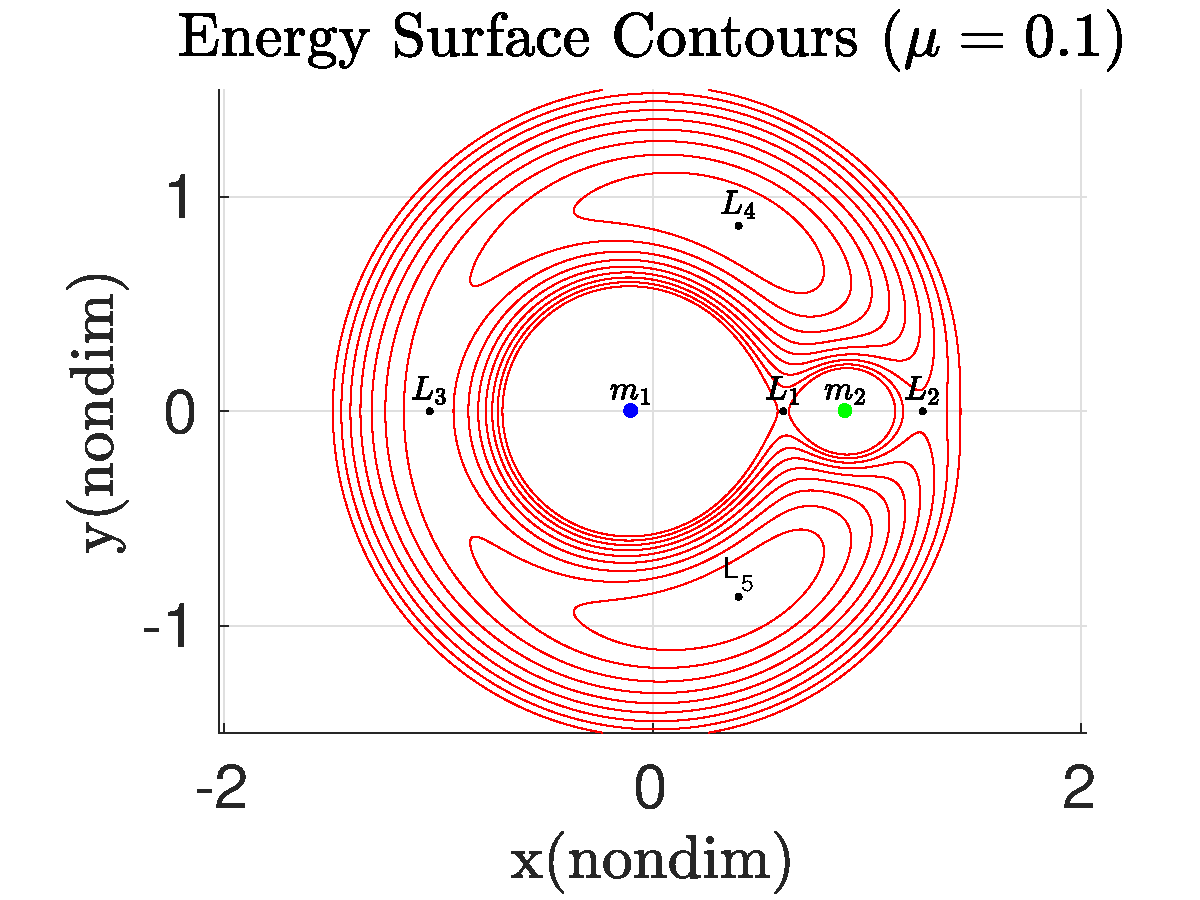
\includegraphics[width=0.75\textwidth]{./figures/2017_JAS/energy_contours.pdf}
        \caption[Jacobi integral]{Contour plot of Jacobi integral: Zero velocity curves of constant Jacobi integral. A particle with fixed energy level cannot cross the contour lines and is therefore limited to specific regions of the phase space. }
        \label{fig:energy_contour}
\end{figure} 

\subsubsection{Invariant Manifolds and \Poincare Map}\label{sec:invariant_manifold}
Dynamics systems theory has been applied to the design of control-free maneuvers in the restricted three-body problem~\cite{koon2011}.
As previously introduced in~\Cref{sec:jacobi}, there exist five equilibrium points in the equations of motion for the three-body problem.
It has been shown that the local orbit structure near the Lagrange points gives rise to families of periodic orbits as well as the stable and unstable manifolds of these periodic orbits.
This rich structure is globally connected and gives rise to a dynamical chain which allows trajectories to pass through the phase space~\cite{koon2011,conley1968}.
The manifold structure associated with periodic orbits about the \( L_1 \) and \( L_2 \) Lagrange points are critical to the understanding of the motion of spacecraft as well as comets/asteroids.
In addition, the stable and unstable manifolds serve as the boundaries of the phase space region that allow for the transport between realms in a single three-body system or between multiple three-body systems.
These invariant manifolds only exist as a result of the dynamic formulation of the three-body problem in a rotating reference frame. 
Invariant manifolds serve as a higher dimensional generalization of the concept of seperatrices from linear systems as applied to the case of nonlinear systems. 

\Poincare maps are a useful tool in the analysis of the flow near periodic orbits in the three-body problem.
We let \( \Sigma \) define a hypersurface of section chosen such that all trajectories in the vicinity of a state \( \vc{q} \in \Sigma \) cross \( \Sigma \) transversely and in the same direction.
A \Poincare map, \( P(\vc{q}) = \phi(T;\vc{q}) \), maps the state of a trajectory from one intersection to the next.
Choosing a section in this manner results in a \Poincare section as shown in~\cref{fig:poincare_map}.
In~\cref{fig:poincare_map} we show two examples of periodic trajectories intersecting the \Poincare section. 
Periodic solutions will appear as fixed points on the section, such as \( q_0, q_1 \) in~\cref{fig:poincare_map}, while stable or unstable trajectories become clearly visible by viewing successive intersections of the section.
This allows for greater insight into the stability and dynamics of periodic solutions of a dynamic system as a fixed point on the \Poincare section corresponds to a periodic orbit while movement on the section is associate with the stability of neighboring trajectories. 
For example, \Poincare maps have been used to prove the existence of homoclinic orbits, which are orbits both forward and backward asymptotic to a single unstable periodic orbit, and heteroclinic orbits, which join different periodic orbits~\cite{conley1968,koon2000b}.
These dynamic features have been shown to play a vital role in the movement of natural bodies as well as critical for spacecraft missions~\cite{gomez2001,lo1997}.

\begin{figure}
    \centering
    \includegraphics[width=\textwidth]{tikz/poincare_map.tikz}
    \caption{Diagram of the \Poincare map: Periodic orbits will appear as fixed points on the \Poincare section \( \Sigma \). Stability of periodic orbits is clearly visible on the section as successive intersections approach or depart a fixed point.\label{fig:poincare_map}}
\end{figure}
% drawbacks of this approach on how we seek to improve upon it
Combining invariant manifolds and an appropriate \Poincare section provides a conceptually simple manner to determine trajectories which connect wide regions of the phase space.
However, the results previously developed are highly case specific and difficult to generalize to arbitrary transfers.
Also, these results are based on control-free trajectories which rely on the underlying structure of the three-body system.
In addition, transfer orbits along an invariant manifold require large time of flights which may be undesirable for time critical missions.
The addition of low-thrust propulsion offers the potential of reduced transit times and the ability to depart from the free motion trajectory to allow for increased transfer opportunities. 
In this paper, we formulate an optimal control problem to generate the reachable set of the spacecraft.
We compute the reachable set on an appropriate \Poincare section and use this to design a transfer trajectory.


\section{Transfer Design around Small Bodies}\label{sec:sc_eoms}

The motion of a massless particle, or spacecraft, about small body shares many similarities with that of the three-body problem.
As is typical in the three-body problem, the equations of motion are usually represented in a uniformly rotating frame aligned with the two primaries.
Similarly, the equations of motion about a small body are also defined in a body-fixed frame with uniform rotation.
In this reference frame, the gravitational potential field is time invariant and only a function of the position of the particle.
In addition, since the rotational rate of the small body is constant, the equations of motion are time invariant.
Finally, the use of the rotating reference frame allows for much greater insight into the dynamic structure of the behavior around the small body.
Here we consider another representation of the dynamics of a spacecraft around a small body which is a slight reformulation of the translational motion presented in~\cref{sec:asteroid_dumbbell_eoms}.
We only treat the translational motion of the spacecraft with respect to the small body instead of the full coupled equations of motion introduced in~\cref{sec:asteroid_dumbbell_eoms}.
The primary use for low thrust transfers is for large scale orbital transfers.
When far from the small body the impact of the irregular shape and rotational state of the spacecraft become less critical to the dynamics.

We utilize the small body fixed frame, \( \fvec{i} \), originating at the center of mass of the small body.
The body-fixed reference frame is composed of the unit vectors \( \fvec{1} , \fvec{2}, \fvec{3} \), which are aligned along the principal axes of smallest, intermediate, and largest moment of inertia, respectively.
From~\cref{sec:asteroid_dumbbell_eoms}, the translational equations of relative motion are given as
\begin{align*}
    \dot{x}_r &= \rvel - \hat{\Omega}_A \rpos, \\
     \dot{v}_r  &= \hat{\Omega}_A \rvel +  \deriv{U}{\rpos},
\end{align*}
where the relative velocity \( \rvel \) is defined as the representation of the inertial velocity in the small body fixed frame, \( \rvel = \aatt^T \dot{\ipos}\).
The position of the spacecraft in the inertial frame is given by \( \ipos \) while the position with respect to the small body frame is \( r = \rpos = \aatt^T \ipos \).
In the \gls{rf2bp}, we consider the time rate of change of the position with respect to the small body frame and define the velocity as \( \dot{r} = \aatt^T \dot{\ipos} - \hat{\Omega}_A r \).
Using this substitution, the body-fixed equations of motion of a massless particle about an arbitrarily rotating small body are given by
\begin{align}\label{eq:body_eoms}
    \ddot{\vc{r}} + 2 \vc{\Omega}_A \times \dot{\vc{r}} + \vc{\Omega}_A \times \parenth{ \vc{\Omega}_A \times \vc{r} } + \dot{\vc{\Omega}}_A \times \vc{r} = \nabla U(\vc{r}) ,
\end{align}
where \( \vc{\Omega}_A \in \R^{3 \times 1}\) is the instantaneous angular velocity vector of the small body represented in the body-fixed frame, \( \vc{r} \) is the position of the particle in the body-fixed frame, and \( \nabla U(\vc{r}) \) is the gradient of the gravitational potential~\cite{scheeres2012a}.
We assume that the small body rotates at a uniform rate, \( \norm{\vc{\Omega}_A} = \omega \in \R^1 \), about the axis of the maximum moment of inertia, i.e.\ \( \vc{\Omega}_A = \omega \hat{\fvec{3}}\).
As a result, we can represent the equations of motion in scalar form as
\begin{align} \label{eq:eoms}
    \begin{split}
        \ddot{x} - 2 \omega \dot{y} - \omega^2 y &= U_x , \\
        \ddot{y} + 2 \omega \dot{x} - \omega^2 x &= U_y , \\
        \ddot{z} &= U_z .
    \end{split}
\end{align}

In this situation, the state is defined as \( \vc{x} = \bracket{\vc{r}~\>\vc{v}}^T \in \R^{6 \times 1}\) with \(\vc{r} = \bracket{x~\>y~\>z}^T \in \R^{3\times1}\) and \(\vc{v}= \bracket{ \dot{x}~\>\dot{y}~\>\dot{z} }^T \in \R^{3\times1}\) representing the position and velocity with respect to the body-fixed frame, respectively.
We further assume that our spacecraft is capable of exerting a translational acceleration, \( \vc{u} \in \R^{3\times1} \), in any direction, while subject to a maximum magnitude constraint, \( \norm{\vc{u}} \leq u_m \).
This is typical of many spacecraft which offer full rotational freedom and can direct a potentially varying force or acceleration in any direction.
The equations of motion may be rewritten in state space form as
\begin{align}\label{eq:state_space_eoms}
    \begin{bmatrix} \dot{\vc{r}} \\ \dot{\vc{v}} \end{bmatrix} &=
    \begin{bmatrix}\vc{v} \\ \vc{g} \parenth{\vc{r}} + \vc{h}\parenth{\vc{v}} + \vc{u} \end{bmatrix} ,
\end{align}
where the terms \(\vc{g} \parenth{\vc{r}} \) and \( \vc{h}\parenth{\vc{v}} \) are given by
\begin{align}\label{eq:state_space_terms}
    \vc{g}\parenth{\vc{r}} = \begin{bmatrix}  U_x + \omega^2 x \\ U_y + \omega^2 y \\ U_z \end{bmatrix} ,\quad
    \vc{h}\parenth{\vc{r}} = \begin{bmatrix} 2 \omega \dot{y} \\ -2 \omega \dot{x} \\ 0 \end{bmatrix} .
\end{align}

Since we assume that the small body is uniformly rotating, the equations of motion are time invariant when represented in the body-fixed frame.
In addition, there exists an integral of motion, or a conserved quantity, that is constant for all motion of a particle.
Similar to the three-body problem, the Jacobi constant for the \gls{rf2bp} is given by
\begin{align}\label{eq:jacobi}
    J \parenth{\vc{r}, \vc{v}} = \frac{1}{2} \omega^2 \parenth{x^2 + y^2} + U(\vc{r}) - \frac{1}{2} \parenth{\dot{x}^2 + \dot{y}^2 + \dot{z}^2} .
\end{align}
The Jacobi constant functions in a similar manner as used in three-body problem~\cite{szebehely1967}.
We can define zero-velocity surfaces using the Jacobi constant by fixing the value to a desired constant.
The zero-velocity surfaces are the locus of points where the kinetic energy and hence velocity vanishes.
Just as in the three-body problem, the Jacobi constant in~\cref{eq:jacobi} divides the phase space into distinct realms of possible motion.
Similarly, there exist, in general, four equilibrium points and also their associated stable and unstable manifolds~\cite{scheeres1996,scheeres1994}.
The properties of these manifolds play a critical role in the dynamics of trajectories in their vicinity.

\section{Optimal Control Formulation for Reachability Sets}\label{sec:optimal_control}
% introduce method
In this section, an optimal control formulation is presented to determine the reachability set on a \Poincare section.
This reachability set is then used to define transfers in both the \gls{pcrtbp} and \gls{rf2bp}.
Our formulation is based on the concept of the reachability set on a \Poincare section.
This method allows one to easily determine potential transfer opportunities by finding set intersections on a lower dimensional space and greatly reduces the design process.
The addition of continuous low thrust propulsion extends the control free design process developed previously and allows for a greater range of potential transfers with a reduced time of flight.
The process is first derived for the \gls{pcrtbp} and then expanded to the higher dimensional case around a small body in the \gls{rf2bp}.

\subsection{Reachability Set}\label{sec:reachability_set}
% discuss reachability and application to space system
Reachability theory provides a framework to evaluate control capability and safety.  
The reachable set contains all possible trajectories that are achievable over a fixed time horizon from a defined initial condition, subject to the operational constraints of the system.
Reachability theory has been applied to aerospace systems such as collision avoidance, safety planning, and performance characterization.
The theory formally supporting reachability has been extensively developed and is directly derivable from optimal control theory~\cite{varaiya2000,lygeros2002,lygeros2004}.
More recently, reachability theory has recently been applied to space systems~\cite{holzinger2009,komendera2012a,dellnitz2006}.
Computation of the reachable set for a system involves solving the Hamilton-Jacobi partial differential equation or satisfying a dynamic programming principle.
Analytical computation of reachable sets is an ongoing problem and is only possible for certain classes of systems.
Typically, numerical methods are used to generate approximations of the reachability set, but are generally limited by the dimensionality of the problem.
 
Computation of reachable sets is critical to space situational awareness, rendezvous and proximity operations, and orbit determination operations.
Specifically, maintaining accurate estimates of a spacecraft state over extended periods is not trivial.
The challenge is increased for multiple spacecraft operating in close proximity or when there are long periods of time between measurements.
Coupling the ability for continuous low-thrust propulsion between measurements increases the measurement association complexity.
Computing the reachability set given estimated states and control authorities allows one to better correlate subsequent measurements or determine sensor pointing regions in the event of a lost spacecraft. 


\subsection{Optimal Control Formulation}\label{sec:optimal_control}
In this paper, we seek to approximate the reachability set on a \Poincare section by solving a related optimal control problem. 
We choose our \Poincare section in a similar manner to those used previously for the design of transfers via invariant manifolds.
The \Poincare section is chosen to intersect transversally with trajectories emanating from the initial orbit. 
In the case of a periodic orbit the trajectories will cross the \Poincare section at two distinct fixed points every half period.
The main idea is that the addition of low thrust propulsion allows us to enlarge the set of trajectories achievable in the \Poincare section. 
\Cref{fig:reachability_set} illustrates how, without any control input, trajectories will intersect with the \Poincare section at \( \vecbf{x}_n \). 
However, the addition of low thrust propulsion allows the spacecraft to depart from the natural dynamics and intersect the \Poincare section at a different location.
We use a cost function to define a distance metric on the \Poincare section from the control-free intersection to an intersection under the influence of the control input.
Maximization of this distance along varying directions enables us to generate the largest reachability set under the bounded control input.
In~\cref{fig:reachability_set} the reachable set is shown as a circular region on the \Poincare section.
In practice, the reachable set will be of a general shape and also higher dimensional in the nonplanar case.
\begin{figure}
        \centering
        \includegraphics[width=\textwidth]{tikz/reachability_set.tikz}
        \caption{Reachability set on a \Poincare section: Pictorial representation of the reachability set (blue circle) on the \Poincare section, \(\Sigma\). 
            The terminal state, \( x_n\), is the intersection without any control input. 
            Adding a control input allows for the terminal state, \( x_f \), to be displaced by some distance/cost \( J \) as measured on the section.
            We parameterize a specific direction on the section with the angles \( \theta_d\) and seek to maximize the distance between \( x_f \) and \( x_n \).
            Computation of the maximum distance, or reachability, for a variety angles gives a discrete approximation of the reachability set.\label{fig:reachability_set}}
\end{figure}

We define the \Poincare section along the horizontal axis, which is equivalent to the surface \( y = 0 \), and given by
\begin{align}
        \Sigma = \braces{ ( x, \dot{x}) \, | \, y = 0} . 
        \label{eqn:poincare_section}
\end{align}
This is similar to the previous work in determining homoclinic orbits in the three-body problem~\cite{llibre1985,koon2011}.
Previous analytical results have shown that homoclinic orbits intersect transversally in the \( (x, \dot{x} ) \) space on the plane \( y = 0 \).
We seek to compliment these results with the addition of low thrust propulsion to maximize the reachable set on the \Poincare section.
Placing our section at \( y = 0\) ensures that all trajectories will intersect our section.
An optimal control problem is defined by a  cost function
\begin{equation}
        J = -\frac{1}{2} \left( \vc{x}(N) - \vc{x}_{n}(N)\right)^T 
        \left[
        \begin{array}{cccc}
                1 & 0& 0& 0 \\
                 0& 0& 0& 0\\
                 0 & 0 & 1 &0\\
                 0 & 0& 0& 0
        \end{array}
        \right]
        \left( \vc{x}(N) - \vc{x}_{n}(N)\right) = \phi(\vc{x}(N),\vc{x}_n(N)) \, .
        \label{eq:cost}
\end{equation}
The term \( \vc{x}_n(N) \) is the final state of a control-free trajectory while the term \( \vc{x}(N)\) is the final state under the influence of the control input.
Maximization of the distance between \( \vc{x}_n \) and \(\vc{x} \), on the \Poincare section defined in~\cref{eqn:poincare_section} at the terminal time \( t_f = N \), is equivalent to the minimization of \( J \) defined in~\cref{eq:cost}.
The \Poincare section is defined through the use of appropriate terminal constraints given by
\begin{subequations}
\begin{align}
    v_1( \vc{x}(N) ) &= y(N) = 0 \, , \\ 
    v_2 ( \vc{x}(N) )&=  \frac{\dot{x}(N) - \dot{x}_n(N) }{x(N) -x_n(N) } - \tan{\theta_d} = 0\, , \\
         0 &\geq\vc{u}^T \vc{u} - u_{max}^2 \, ,
\end{align}
    \label{eq:constraints}
\end{subequations}
where the angle \( \theta_d\) defines a direction in which we wish to maximize the reachability set on the \Poincare section.
The maximum control thrust magnitude is defined by \( u_{max} \) and is non-dimensionalized by the characteristic units of length, mass, and time.
The goal is to determine the control input \( \vc{u}_k\) such that the cost function~\cref{eq:cost} is minimized subject to the state equations of motion~\cref{eqn:cont_dyn} and constraints~\cref{eq:constraints}.

Application of the Euler-Lagrange equations allows us to derive the necessary conditions for optimality~\cite{bryson1975}.
This results in an optimal control problem and the necessary conditions are given as
\begin{subequations}\label{eq:necc_cond}
\begin{align}
    \dot{\vc{\lambda}} &= - \deriv{H}{\vc{x}}, \\
        0 &=  \deriv{H}{\vc{u}} \, , \label{eqn:control_necc_cond}\\
        0 &= \deriv{\phi}{\vc{x}}^T + \deriv{\vc{v}}{\vc{x}}^T \vc{\beta}  - \vc{\lambda}^T(N) \, ,  
\end{align}
\end{subequations}
where the Hamiltonian \(H\) is defined as
\begin{equation}
        H = \vc{\lambda}^T \vc{f}(\vc{x}, \vc{u}) \, ,
        \label{eq:hamiltonian_opt}
\end{equation}
and \( \vc{\lambda} \in \R^{4 \times 1} \) is the costate and \(\vecbf{\beta} \in \R^{2 \times 1} \) are the additional Lagrange multipliers associated with the terminal constraints in~\cref{eq:constraints}.
The state dynamics are represented by \( \vc{f}(\vc{x}_k, \vc{\lambda}_k ) \) after substituting~\cref{eqn:control_necc_cond} into~\cref{eqn:cont_dyn}.
This indirect optimal control formulation leads to a two point boundary value problem with split boundary conditions. 
By sweeping the angle \( \theta_d \) one can approximate the reachable set on the \Poincare section subject to the bounded control input. 

The optimal control formulation presented in this section results in a \gls{tpbvp}. 
There exist many methods to solve \glspl{tpbvp} such as gradient, quasilinearization, and shooting methods~\cite{bryson1975,kirk2012}.
Shooting methods are common in astrodynamic trajectory design problems and relatively simple to implement.
In the shooting method, initial conditions are varied such that a terminal constraint is satisfied, similar to the way an archer modifies the bow in order to more accurately strike a target. 
Consider the vector of initial conditions, \( \vc{\chi} = \braces{\vc{x}_0, \vc{\lambda}_0}\), which is varied to satisfy some terminal constraints of the form \( \vc{G}(\vc{\chi}) = \braces{\vc{x}_t - \vc{x}_n} = 0 \).
The free variables at the terminal time are computed by propagation of \( \vc{\chi} \) over the selected time horizon. 
At the terminal time, the constraint vector is calculated and if not satisfied \( \vc{\chi}\) is varied.
Rather than numerical integration over the entire time interval, multiple shooting segments the interval into several smaller sub-arcs~\cite{stoer2013}.
This multiple shooting approach incorporates additional interior constraints but reduces the sensitivity of the costates along each sub-arc.
The use of the multiple shooting method reduces the sensitivity of changes in the initial costate at the expense of additional design variables, but has been shown to provide more stable and robust solutions~\cite{ozimek2010a}.

\begin{figure}
    \centering
    \includegraphics[width=\textwidth]{tikz/multiple_shooting.tikz}
    \caption{Schematic diagram of the multiple shooting method:
        The complete trajectory is split into a number of sub-segments, and additional interior constraints are included to ensure state and costate continuity.
        Splitting the optimal trajectory into short segments reduces the sensitivity of terminal states to variations of the initial states.\label{fig:multiple shooting}}
\end{figure}

In~\cref{fig:multiple shooting}, we show a schematic representation of the multiple shooting procedure.
We split the optimal control horizon into equal length subsegments such that the length of each segment is \( \frac{k}{n} \), where \( k, n \) are the total number of steps and number of stages, respectively.
Similarly, we divide the state and costate trajectories into \( n \) equal segments. 
To ensure continuity, additional interior constraints are incorporated as
\begin{align}\label{eq:interior_constraints}
        \vc{x}_1^{-} - \vc{x}_1^{+} &= 0 , \nonumber\\ 
        \vc{\lambda}_1^{-} - \vc{\lambda}_1^{+} &= 0 , \nonumber\\
        \vc{x}_2^{-} - \vc{x}_2^{+} &= 0 , \nonumber\\ 
        \vc{\lambda}_2^{-} - \vc{\lambda}_2^{+} &= 0 , \nonumber\\
        &\vdots \nonumber \nonumber\\
        \vc{x}_{n-1}^{-} - \vc{x}_{n-1}^{+} &= 0 , \nonumber\\ 
        \vc{\lambda}_{n-1}^{-} - \vc{\lambda}_{n-1}^{+} &= 0.
\end{align}
Using the multiple shooting method reduces the sensitivity of the terminal states, \( \vc{x}_i^{+}, \vc{\lambda}_i^{+}\), to variations of the initial states, \(\vc{x}_{i-1}^{-}, \vc{\lambda}_{i-1}^{-}\).
As a result, the design vector \( \vc{\chi} \) is augmented with the additional interior initial conditions, \( \vc{x}_i^{-}, \vc{\lambda}^{-}\).
Similarly, the constraint vector is augmented with the additional interior constraints defined in~\cref{eq:interior_constraints}.
Based on experimentation, we use four stages in our multiple shooting method.
This provided the best performance and convergence stability while minimizing the difficulties in additional interior constraints.
The multiple shooting algorithm now varies the design vector \( \vc{\chi}\) to ensure that the constraints in \( \vc{G}(\vc{\chi}) \) are satisfied.
In this work, we use the Matlab nonlinear solver \texttt{fsolve} to solve the system of nonlinear equations defined by the multiple shooting algorithm with a convergence tolerance of \num{1e-5}.
Within \texttt{fsolve}, we use the trust-region dogleg solver which makes use of the Powell dogleg procedure for computing a step direction and magnitude to minimize successive iterations of the solver.
The numerical results are specific to the choice of nonlinear solver, and different tolerances or software tools may result in slight changes.

% TODO Add numerical examples of the three-body problem
\section{Numerical Examples of Transfers using Reachability Sets}\label{sec:simulation}
We present two numerical simulations in the Earth-Moon system to demonstrate the transfer procedure.
These simulations enable the spacecraft to depart from the natural dynamics through the use of low-thrust propulsion.
The reachability set on the \Poincare section allows for a straightforward method of determining transfer opportunities.
The first example is a transfer from a periodic orbit of the \( L_1 \) Lagrange point to a fixed orbit of the moon.
This example uses a single iteration of the reachable set computation in the design of the transfer.
The second example is a transfer from geostationary orbit of the Earth to a period orbit of \( L_1 \). 
This examples demonstrates the ability to extend the reachability process to multiple iterations, to allow for a much larger and more general transfer.
With both examples it is possible to depart from the vicinity of the Earth to a Moon orbit via a series of reachable sets defined on \Poincare sections.
The numerical examples presented in this section satisfy the necessary conditions for local optimality and obtaining a globally optimal solution is considered beyond the scope of this paper.
Next, the results are extended from the planar problem to three dimensions with a simulation about asteroid 4769 Castlia.
This numerical examples demonstrates the extension of the method to the more complicated dynamic enviornment around an asteroid.

\subsection{Three Body Examples}

\paragraph{Periodic Orbit Transfer}\label{sec:periodic_orbit_transfer}
The first objective is to design a transfer trajectory from a planar periodic orbit about the \( L_1\) Lagrange point to a bounded orbit in the vicinity of the Moon.
The target region is created by choosing an initial condition of \( x_0 = \begin{bmatrix}1.05 & 0 & 0 & 0.35 \end{bmatrix}^T \) with \( \mu = 0.0125 \).
The target set is propagated over a period of \( t = \num{20} \) in non-dimensional units which corresponds to approximately \num{1.5} years.
\begin{figure}[htbp]
   \centering
   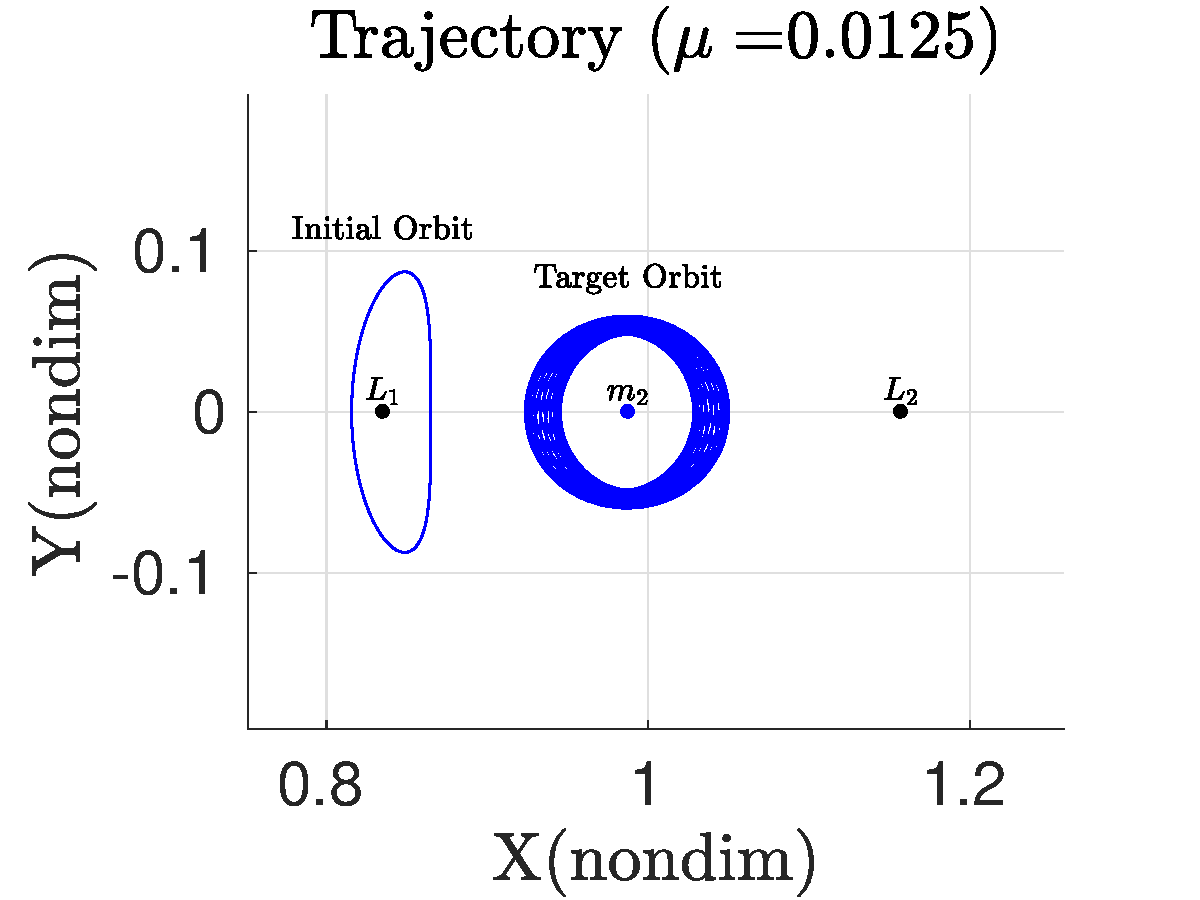
\includegraphics[width=0.5\textwidth]{figures/2017_JAS/moon_orbit.pdf} % requires the graphicx package
   \caption{\(L_1\) periodic orbit transfer to orbit of the Moon: Example scenario demonstrating the initial and target orbit.
   Without the low-thrust propulsion, the spacecraft is constrained to the initial periodic orbit. 
   We determine the reachability set to find a transfer trajectory to the target orbit about the moon.}
   \label{fig:moon_orbit}
\end{figure}
\Cref{fig:moon_orbit} shows that the target set remains in the vicinity of the Moon, or \( m_2\), in the rotating reference frame. 
This type of orbit would be useful for a variety of mission scenarios.
For example, a series of communication satellites could be placed in this type of orbit. 
The bounded trajectories of the vehicles and constant line of sight to both the Moon and the Earth would allow for constant communication for future manned missions and potential habitats.
The initial set is a planar periodic orbit about \( L_1\), which is generated using the process of differential correction of a linear approximation~\cite{koon2011}.

% invariant manifold transfer
As a source for comparison, the method of using invariant manifolds, introduced in~\cite{koon2011}, is implemented.
As described in~\cref{sec:invariant_manifold}, these invariant manifolds are the set of trajectories that either asymptotically arrive or depart the periodic orbit. 
We generate the unstable manifold associated with the initial planar periodic orbit.
We numerically propagate the unstable manifold forward in time until the trajectories intersect the \Poincare section \( y = 0 \).
\Cref{fig:manifold_trajectory} shows the unstable invariant manifold generated from the initial \( L_1\) periodic orbit. 
The blue points in~\cref{fig:manifold_poincare} are the intersections of the target Moon orbit and the \Poincare section.
The two circular regions are the ascending (right) and descending (left) intersections of the target orbit and \Poincare section.
The green points in~\cref{fig:manifold_poincare} are intersections of the unstable manifold from~\cref{fig:manifold_trajectory} with the \Poincare section \( y = 0 \).
Only a single branch of the invariant manifold intersects with the ascending region of the target orbit.
There are no intersections of the invariant manifold with the descending region of the target orbit.
The numerical values associated with the green points denote the required time of flight along the invariant manifold in non-dimensional units.
The required travel time for a transfer using the unstable invariant manifold is  approximately \( t_f \approx 3.1\) non-dimensional time units.
\begin{figure} 
        \centering 
        \begin{subfigure}[htbp]{0.5\textwidth} 
            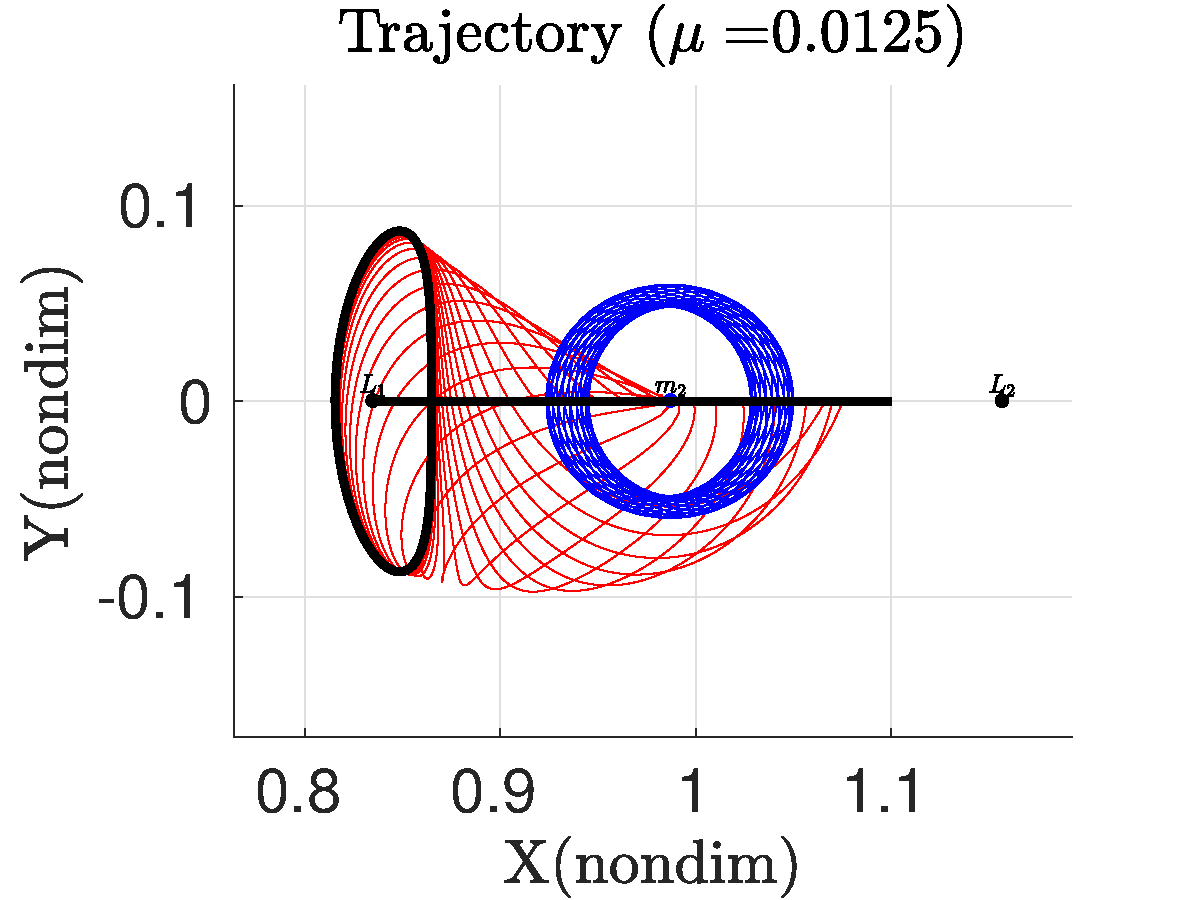
\includegraphics[width=\textwidth]{figures/2017_JAS/manifold_trajectory} 
                \caption{Position space view of invariant manifold} \label{fig:manifold_trajectory} 
        \end{subfigure}~ %
        \begin{subfigure}[htbp]{0.5\textwidth} 
            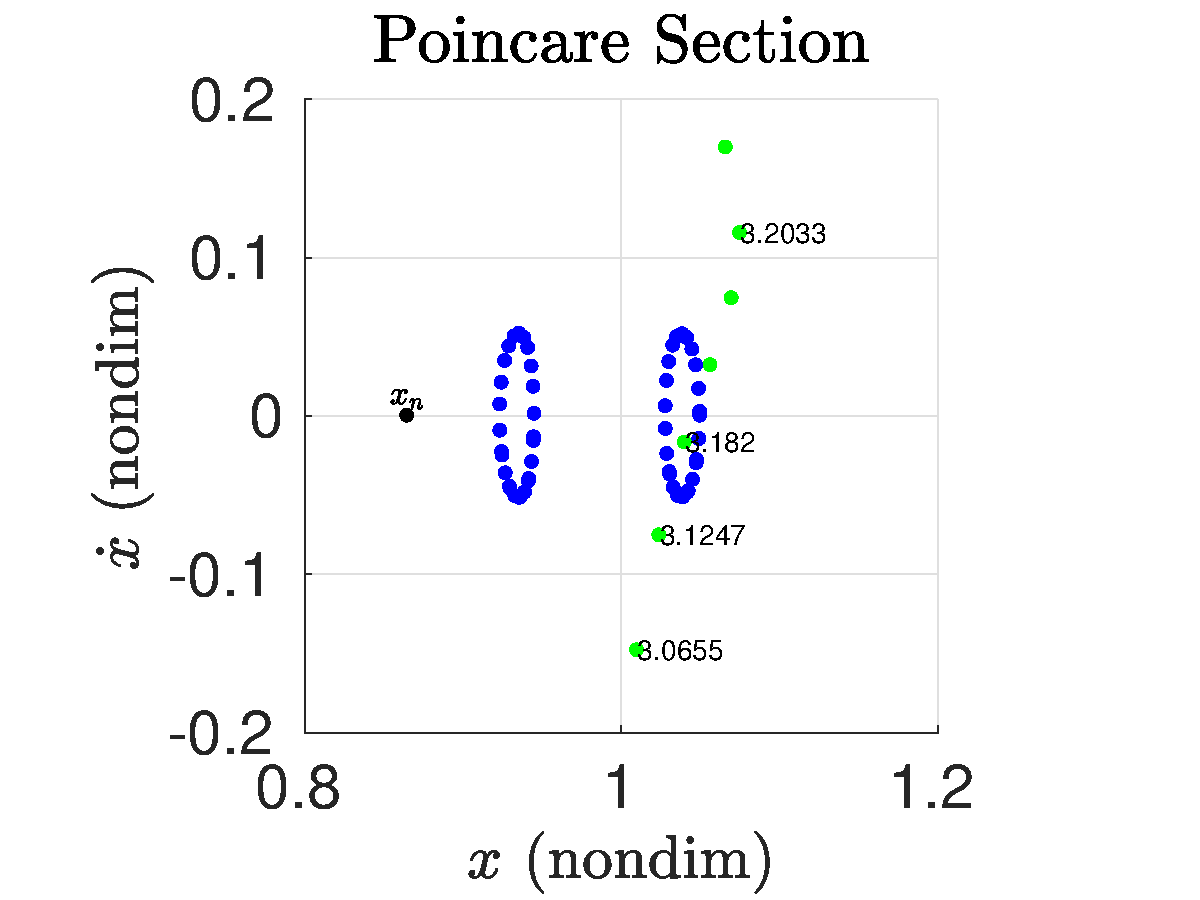
\includegraphics[width=\textwidth]{figures/2017_JAS/manifold_poincare} 
                \caption{\Poincare intersection of invariant manifold (green), target orbit (blue) and the initial orbit (black)} \label{fig:manifold_poincare} 
        \end{subfigure} 
        \caption{Invariant manifold transfer: An example transfer using the invariant manifolds is shown in both the position and \Poincare spaces.
        The control free transfer from the initial periodic orbit to the target orbit result in a long time of flight. 
    In addition, the manifold only intersects the target orbit on the ascending or far side of the moon.}
        \label{fig:invariant_manifold_transfer} 
\end{figure}

Next, we determine the reachability set with addition of a low-thrust control input over a fixed time horizon.
In~\cref{fig:varying_tf_reachability_sets}, we demonstrate the effect of variations in the choice of maximum control bound and terminal time.
While~\cref{sssec:periodic_orbit_transfer} show a specific example of a transfer design process using the intersection of the reachability set on the \Poincare section.
The analysis presented in the following sections define a maximum magnitude of the thrust as \( u_{m} \) and assume that the trust can be directed arbitrarily within the plane. 
This model is representative of many spacecraft which have a body fixed thruster and attitude control system.
Assuming a fully actuated spacecraft model allows us to decouple the translation and rotational dynamics of the spacecraft.

\paragraph{Reachability Set on the \Poincare section}
From the initial state on the periodic orbit, a series of optimal trajectories are generated to determine the reachable set.
The multiple shooting approach is implemented to solve the optimal control problem. 
We divide the time horizon into two equal length segments. 
The state trajectory is initialized using the free trajectory of the periodic orbit. 
Similarly, the costate trajectory is initialized from an initial guess of \( \vc{\lambda}_0 = \begin{bmatrix} -1 & -1 & -1 & -1\end{bmatrix}^T\) and propagated using the system dynamics.
This results in the initial guess of the design vector \( \vc{\chi} = \begin{bmatrix} \vc{\lambda}_0 & \vc{x}_1^{-} & \vc{\lambda}_1^{-} & \vc{\beta} \end{bmatrix}^T\).
This design vector is then varied to ensure that the necessary conditions of optimality and the interior point constraints are satisfied. 
\Cref{tab:varying_tf} shows the range of terminal times, \( t_f \), and maximum control bound, \( u_m \), which are used to investigate their effect on the subsequent reachable set on the \Poincare section.
\begin{table}
    \centering
    \begin{tabular}{ll}  
        \toprule
        \(t_f\) & \( u_m \) \\
        \midrule
        1.24 & 0.05 \\
        1.30 & 0.25 \\
        1.37 & 0.5 \\
        1.44 & \\
        \bottomrule
    \end{tabular}
    \caption{Combinations for \( t_f \) and \( u_m\) used to generate the reachability sets in~\cref{fig:varying_tf_reachability_sets}~\label{tab:varying_tf}}
\end{table}

The angle \( \theta_d\) in~\cref{eq:constraints} is varied to select a different direction along the \Poincare section to maximize.
We discretely vary the angle over the range \( \ang{0} \leq \theta_d < \ang{360} \) to approximate the reachability set of the spacecraft.
Choosing a new angle \( \theta_d \) corresponds to a different direction as well as a new optimal control problem which is again solved using the multiple shooting approach laid out previously.
Each optimal control solution, corresponding to a discrete value of \( \theta_d \), is solved using \texttt{fsolve} as described earlier. 
Each solution on the reachability set is computed in approximately \SI{2}{\minute} on a desktop computer using an \SI{3.4}{\giga\hertz} Intel i7-3700.
The intersection of the optimal trajectories as well as those of the target Moon orbit with the \Poincare section are shown in~\cref{fig:varying_tf_reachability_sets}.

\begin{figure}
    \subcaptionbox{Position space view of reachability sets\label{fig:varying_tf_trajectory}}{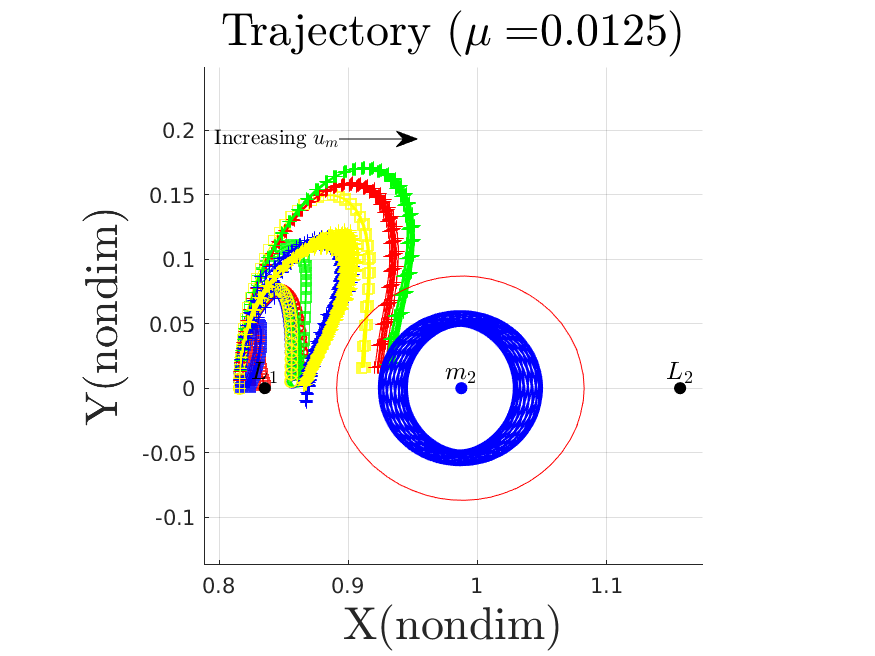
\includegraphics[width=0.5\textwidth]{figures/2017_JAS/trajectory_varying_um.pdf}}~
    \subcaptionbox{\Poincare section view of reachability sets\label{fig:varying_tf_poincare}}{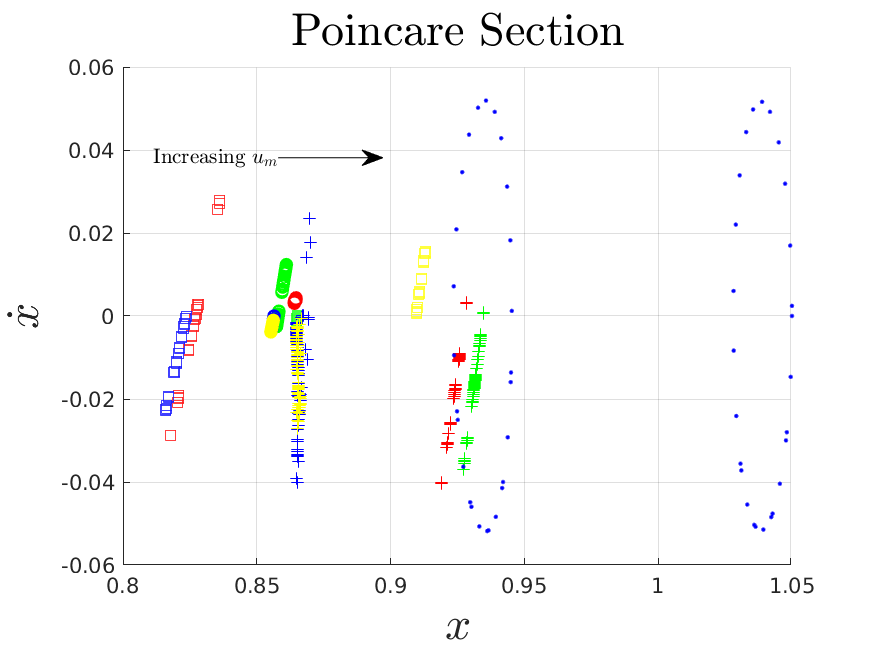
\includegraphics[width=0.5\textwidth]{figures/2017_JAS/poincare_section_varying_um.pdf}}
    \caption{Variation of \( t_f \) and \( u_m\) on the reachability set. 
        Colors, \braces{\text{red}, \text{blue}, \text{green}, \text{yellow}}, are used note increasing \( t_f\) while markers, \braces{\text{circle}, \text{square}, \text{cross}}, are used to denote increasing \(u_m\).
    Increasing the maximum control bound has a large effect and enables the reachability set to intersect the target manifold. 
    Increases in \(t_f\) are less critical and have minimal impact on the distribution of the reachability set on the \Poincare section.~\label{fig:varying_tf_reachability_sets}}
\end{figure}

\Cref{fig:varying_tf_reachability_sets} shows the reachabilty set for twelve combinations of \(t_f\) and \( u_m\) listed in~\cref{tab:varying_tf}.
With a small maximum control bound, \( u_m = \num{0.05} \) shown using square markers, the reachable set is not dramatically changed from that of the no control solution.
The reachable set is denoted using square markers on the left most portion of \cref{fig:varying_tf_poincare}.
Variations of \( t_f\) are indicated using different colors and also demonstrate that this parameters has a smaller impact than changes in \( u_m \).
Increasing the control bound to \( u_m = \num{0.25} \) and \( u_m = \num{0.5} \) shows that the reachable set progressively approaches the target set.

The reachable sets presented in~\cref{fig:varying_tf_reachability_sets} are highly dependent on the initial condition, terminal time, and maximum control bound. 
This example demonstrates that increasing the \( u_m \) results in a larger displacement between the controlled and uncontrolled trajectories.
The reachable set is enlarged from a single point, as shown in~\cref{fig:manifold_poincare} by the black point, to a larger region as shown in~\cref{fig:varying_tf_poincare}.
The choice of \( u_m\), \( t_f \) and initial condition all combine to change the resulting reachability set. 

\paragraph{Transfer to Periodic Orbit}~\label{sssec:periodic_orbit_transfer}
% reachable set transfer
Here we use the results of the preceding section to demonstrate one specific example of a transfer designed using the reachability set.
The acceleration limit is chosen as  \( u_{max} = 0.75 \approx \SI{2}{\milli\meter\per\second\squared} \) in the Earth-Moon system.
Assuming a fixed spacecraft mass of \SI{500}{\kilo\gram}, this model defines a maximum thrust of approximately \SI{1}{\newton}.
Currently, the NASA NEXT xenon thruster is able to provide approximately \SI{0.25}{\newton} of thrust, and a cluster of such engines could be used to provide the desired thrust used in this work~\cite{schmidt2008}.
The trajectories are generated from a fixed initial state of \( \vc{x}_0 = \begin{bmatrix}0.8156 & 0 & 0 & 0.1922 \end{bmatrix}^T \) over a fixed time span of \( t_f = 1.4 \).
This initial state lies on the initial periodic orbit and the time of flight is equivalent to one half period of the initial periodic orbit. 

% discuss reachability set computation
The optimal trajectories, under the influence of the control input \( \vc{u} \), are plotted in red in~\cref{fig:reach_trajectory}.
Initially, the spacecraft is assumed to lie on the periodic orbit.
As a result, the intersection of this periodic orbit with the \Poincare section are two points corresponding to the two crossing of the orbit.
We show the control-free intersection, \( \vc{x}_n \), of the periodic orbit on the \Poincare section in~\cref{fig:manifold_poincare,fig:poincare_compare}
The use of the continuous low thrust propulsion expands the reachable set to region bounded by the red markers in~\cref{fig:poincare_compare}.
The reachable set is an ellipsoidal region with a major axis aligned along \( \theta \approx \ang{70} \) as compared to a fixed point without any control input.
\begin{figure} 
        \centering 
        \begin{subfigure}[htbp]{0.5\textwidth} 
            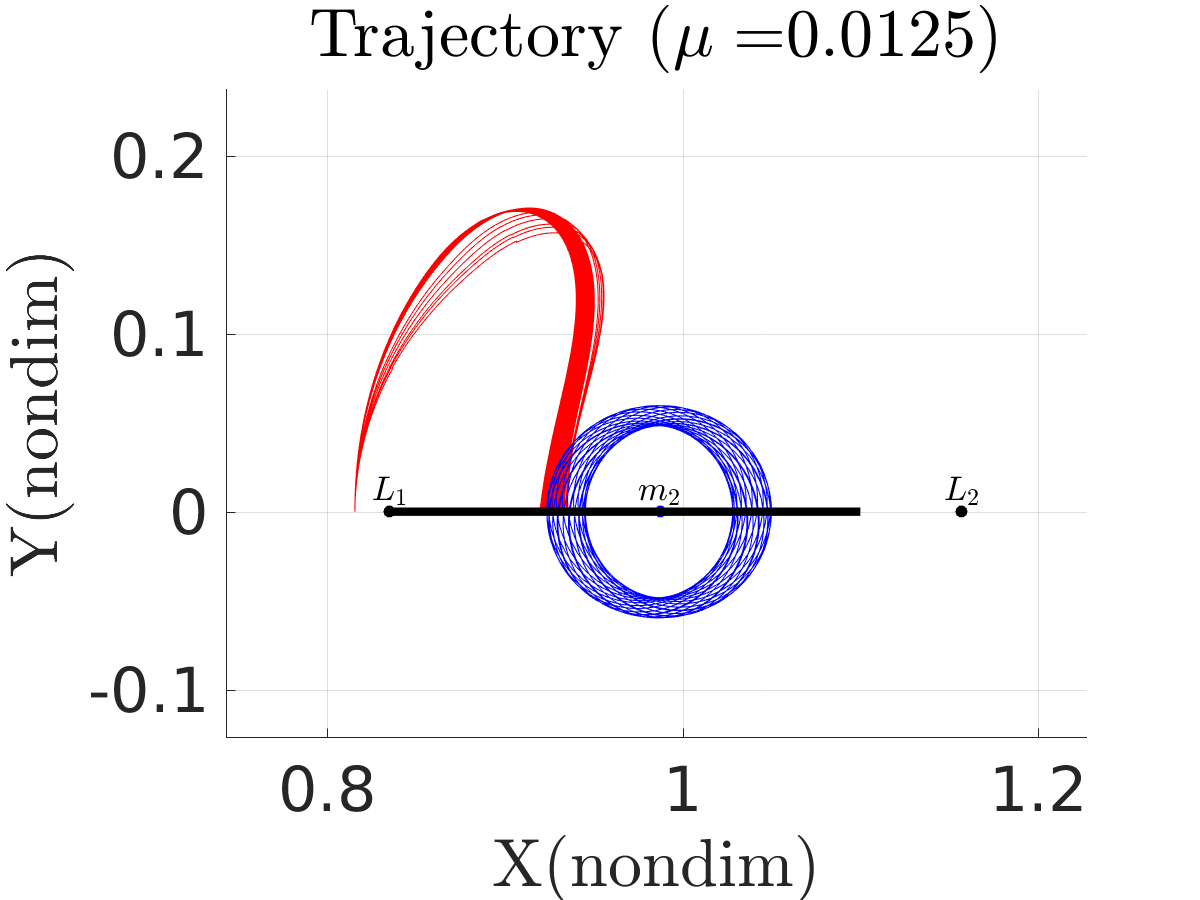
\includegraphics[width=\textwidth]{figures/2017_JAS/reach_trajectory} 
                \caption{Position space view of reachability set} \label{fig:reach_trajectory} 
        \end{subfigure}~ %add desired spacing between images, e. g. ~, \quad, \qquad, \hfill etc. %(or a blank line to force the subfigure onto a new line) 
        \begin{subfigure}[htbp]{0.5\textwidth} 
            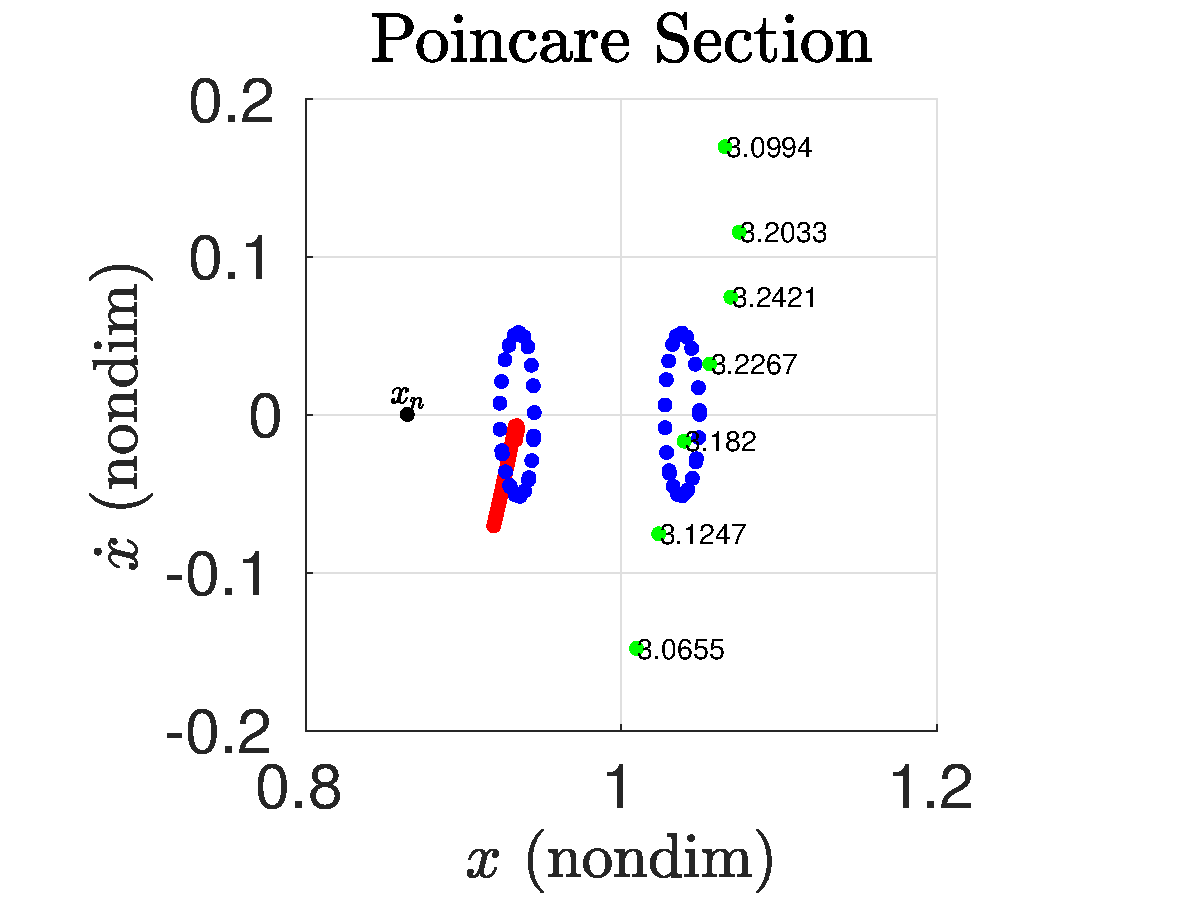
\includegraphics[width=\textwidth]{figures/2017_JAS/poincare_compare} 
                \caption{\Poincare section view of reachability set} \label{fig:poincare_compare} 
        \end{subfigure} %add desired spacing between images, e. g. ~, \quad, \qquad, \hfill etc. %(or a blank line to force the subfigure onto a new line) 
                
        \begin{subfigure}[htbp]{0.5\textwidth} 
            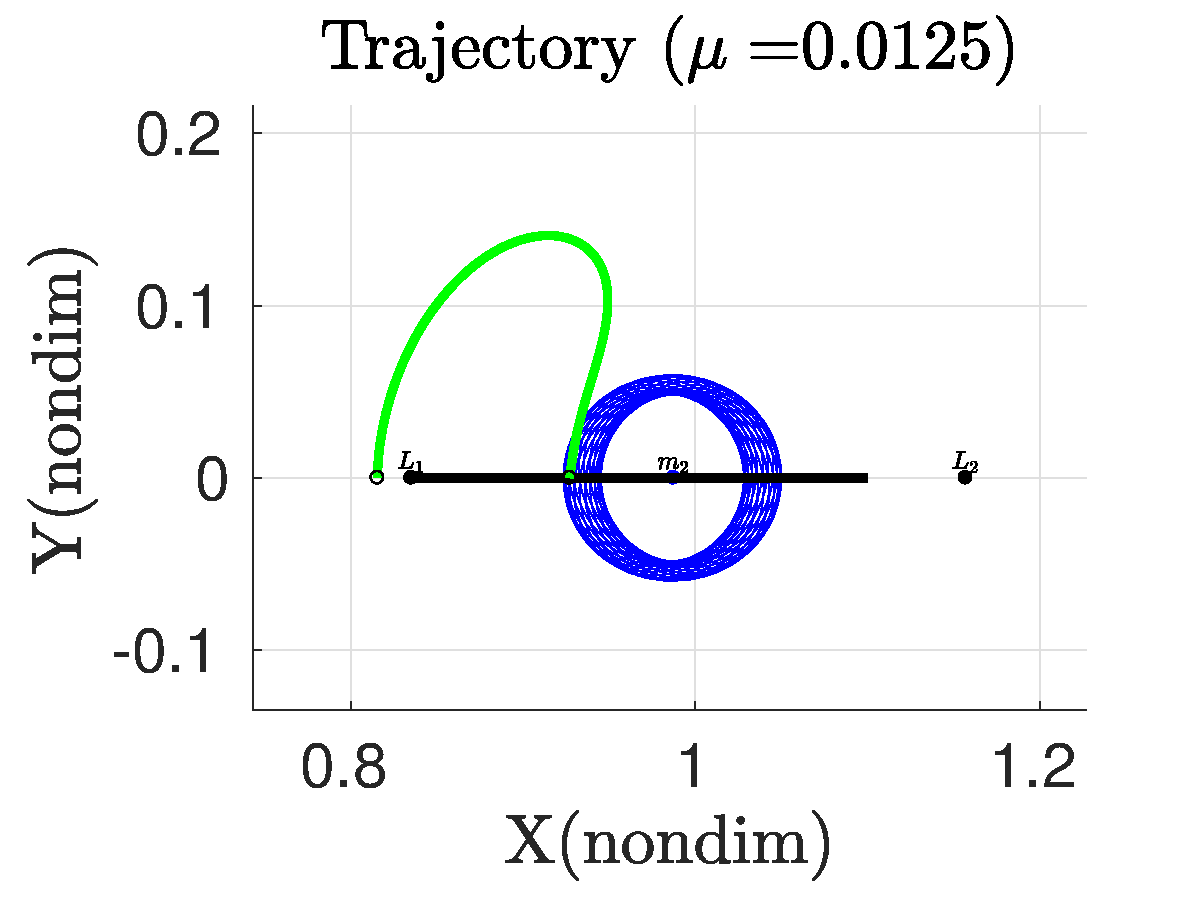
\includegraphics[width=\textwidth]{figures/2017_JAS/reach_transfer} 
                \caption{Transfer trajectory selected from reachability set viewed in the position space} \label{fig:reach_transfer} 
        \end{subfigure}~ 
        \begin{subfigure}[htbp]{0.5\textwidth} 
            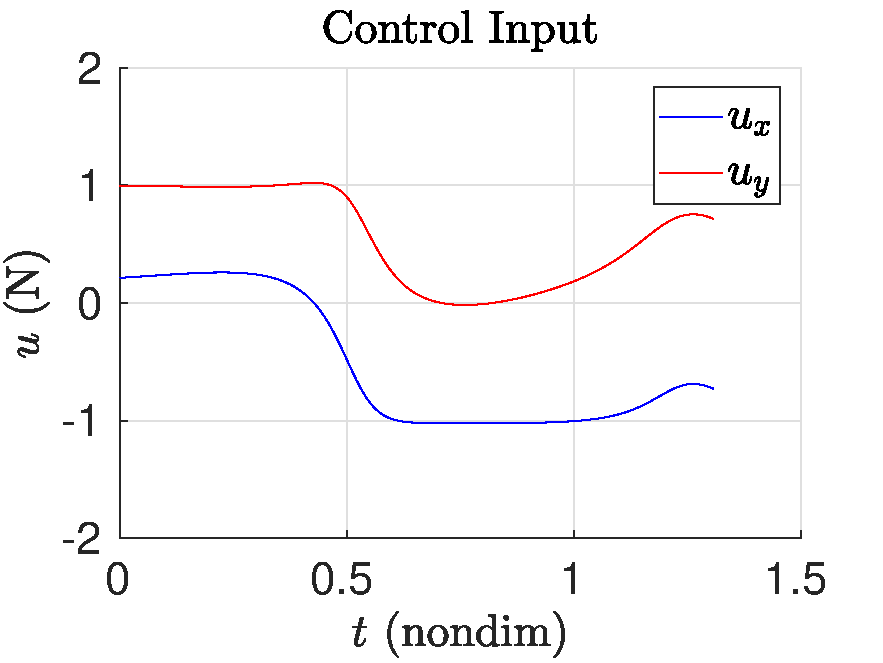
\includegraphics[width=\textwidth]{figures/2017_JAS/control_input_l1} 
                \caption{Control input for the selected transfer trajectory} \label{fig:control_l1} 
        \end{subfigure}~

        \begin{subfigure}[htbp]{0.5\textwidth} 
            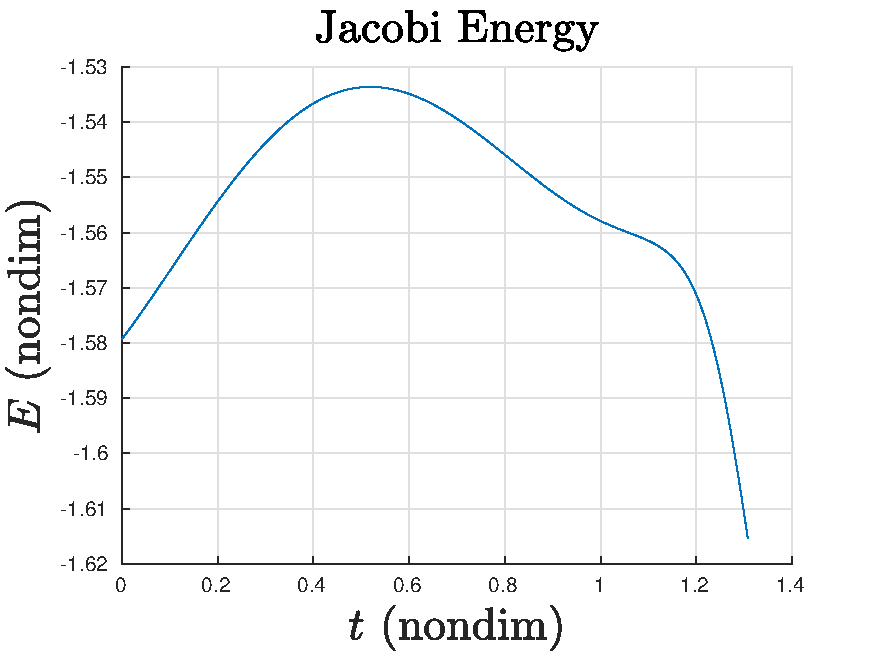
\includegraphics[width=\textwidth, keepaspectratio]{figures/2017_JAS/jacobi.pdf} 
            \caption{Jacobi Energy over transfer \label{fig:jacobi_l1}} 
        \end{subfigure} 

        \caption{\( L_1 \) Reachability set transfer: The low thrust propulsion is used to approximate the reachability set starting from the initial periodic orbit over a fixed time horizon.
            The reachability set is shown in~\cref{fig:reach_trajectory,fig:poincare_compare} in both the position and \Poincare space respectively.
            From this reachability set we chose a trajectory which intersects the target orbit and it is shown in~\cref{fig:reach_transfer}.
        The optimal control to achieve this transfer is shown in~\cref{fig:control_l1}.}
        \label{fig:reachability_set_transfer} 
\end{figure}

% generate the optimal transfer
\Cref{fig:poincare_compare} shows that the reachable set and those of the descending target region intersect.
As both regions are discretely approximated a linear interpolation is used to determine the exact intersection state on the \Poincare section.
This intersection generates a partial target state of \( x_t \text{ and } \dot{x}_t \).
Using the energy level of the target region, defined by~\cref{eq:jacobi}, and the intersection state we can calculate the final component \( \dot{y} \). 
This results in a complete target state \( \vecbf{x}_t \) which lies on the reachable set and on the target orbit. 
A final optimal trajectory is generated such that the \( \vecbf{x}(N) = \vecbf{x}_t \).
This transfer trajectory is denoted by the green path in~\cref{fig:reach_transfer}.
The optimal control input is shown in~\cref{fig:control_l1}. 
The spacecraft achieves the desired target while satisfying the bounded control input.
The Jacobi energy integral, computed using~\cref{eq:jacobi}, is shown in~\cref{fig:jacobi_l1}.
\Cref{fig:jacobi_l1} shows that the vehicle begins with an energy level equal to the periodic orbit and arrives at the target orbit with the appropriate energy.
The first half of the transfer is associated with and increase in energy as the control is used to transition towards the target orbit which is followed by a energy decrease to the target orbit.
This roughly corresponds with the expected optimal solution of a bang-coast-bang type orbital transfer~\cite{kirk2012}.
Convergence statistics associated for this transfer are shown in~\cref{tab:l1_transfer_stats}.
\begin{table}
    \centering
    \begin{tabular}{llr}  
        \toprule
        Metric    & Value \\
        \midrule
        \texttt{fsolve} objective      & \num{6.03e-15}      \\
        \texttt{fsolve} major iterations       & \num{9}      \\
        \texttt{fsolve} first order optimality & \num{1.88e-13} \\
        Optimal cost       & \num{2.09e-31}      \\
        Execution time & \SI{1.49}{\second}       \\
        \bottomrule

    \end{tabular}
    \caption{Convergence statistics for the periodic orbit transfer\label{tab:l1_transfer_stats}}
\end{table}

% compare the invariant manifold method and reachability set
A transfer along the invariant manifold requires on average \( t_f \approx 3.1 \) as compared to \( t_f \approx 1.4 \) for a transfer using low thrust propulsion and the reachable set.
This long time of flight is typical of transfers using invariant manifolds.
The unstable invariant manifold traverses a large region of the phase space and is dependent on the system dynamics. 
In addition, the invariant manifolds asymptotically arrive and depart from the periodic orbit. 
As a result, it may take an arbitrarily long period of time to depart from the vicinity of the periodic orbit.
In addition, only a small portion of the invariant manifold intersects with the target Moon orbit.
In contrast, the low thrust control input we are able to enlarge the reachability set from a single point, \( x_n\) associated with the periodic orbit, to a larger ellipsoidal region shown in red in~\cref{fig:poincare_compare}.
This achieves an intersection with the target orbit with a much lower time of flight as compared to the invariant manifold method.
In addition, by generating the reachability set we are able to compute the required control input to exactly intersect the target orbit.
This avoids having to compute and accomplish a secondary impulsive maneuver to transition from the invariant manifold to the target orbit.

\paragraph{Geostationary Orbit Transfer}
% motivation - may need to compute several reachability sets
There are many situations where a more complicated and extensive orbital transfer is desired. 
In this section, we present a simulation of transferring from a geostationary orbit to a periodic orbit about the \( L_1 \) Lagrange point.
From this location, it is possible to transition to the Moon, as shown in~\cref{sec:periodic_orbit_transfer}, or beyond the Earth-Moon system through the use of invariant manifolds~\cite{koon2011}.
This type of low energy transfer would be most suitable for unmanned spacecraft transitioning from the Earth to the Moon.
The long time of flight would make such a transfer unsuitable for manned missions due to life support constraints.
Future proposals for permanent lunar spacecraft and bases will require frequent supply missions to remain viable. 
Transfers from the Earth to the Lagrange points, through the use of low-thrust electric propulsion, offer an additional and potentially shorter time of flight in comparison to the low-energy transfers which utilize solar perturbations.

\Cref{sec:periodic_orbit_transfer} demonstrated the capability of determining an orbital transfer after locating the intersection of the reachability set and a target orbit.
However, it may not be possible to achieve an intersection on the \Poincare section after a single iteration. 
Since the spacecraft has an upper bounded control input and time of flight the reachability set is finite in size. 
As a result, we present a method of performing several iterations of the reachability set computation. 
A straightforward method is presented which allows for a series of reachability sets to be computed which progressively move the trajectory towards the target.
In this manner, it is possible to determine more complicated transfers by a simple selection of states from the reachability set.
This affords a systematic method of determining general transfer trajectories in the three body problem.

% discuss difficulties in applying direct optimization or the invariant manifold method
It is possible to design arbitrary transfers using either a direct optimization or invariant manifold based approach.
The direct optimization method transforms the optimal control problem into a nonlinear programming problem.
Instead of solving the Euler-Lagrange equations the state and control histories are parameterized and solved through any number of mathematical programming methods.
However, due to this parameterization only an approximate solution, which approximates the true optimal solution in the limit, is feasible. 
On the other hand, our method applies an indirect optimization method.
The necessary conditions for optimality are computed and directly solved in generating the reachability set. 
The use of the reachability set also avoids the issues of selecting a valid initial condition.
We select a state on the maximum reachability set which minimizes the distance toward the target. 
This straightforward approach achieves an optimal trajectory and is used to generate general transfers.

The invariant manifold method is difficult to apply to general orbital transfers. 
The manifolds are associated with periodic orbits in the three-body system. 
In this case, an appropriate periodic orbit must first be determined prior to generating the invariant manifold.
Furthermore, there is no guarantee that the invariant manifold will pass through a desired region of space. 
For example, in the Earth-Moon system the unstable manifolds of periodic orbits about \( L_1 \) do not pass close to the Earth, but rather are beyond the geostationary orbit altitude. 
In addition, determining the intersections between various invariant manifolds is not trivial. 
It requires an appropriate \Poincare~section and the generation of several invariant manifolds.
There is no clear method of selecting the periodic orbits required based on the type of transfer desired. 
Determining an intersection between these invariant manifolds generally requires extended flight times, involving several orbits of the primaries, before an appropriate intersection is found.
As a result, it is difficult to generalize this method to arbitrary transfers in the three-body problem.

% describe initial and target states for this example
This numerical simulation demonstrates the ability of the our approach to determine more general transfer trajectories in the \gls{pcrtbp}. 
We use multiple iterations of the reachability set to achieve a more complicated transfer.
In this manner, it is possible to design arbitrary transfers which are not possible using a single reachability computation.
Initially, it is assumed that the spacecraft lies on a circular geostationary orbit in the non-dimensional Earth-Moon three-body system. 
While the geostationary orbit is not a typical ``parking orbit'' for most spacecraft missions it serves as a convenient altitude to demonstrate our approach.
The geostationary orbit about the Earth is transformed into the rotating reference frame of the Earth-Moon three body problem.
In addition, we non-dimensionalize the initial state to find \( \vc{x}_0 = \begin{bmatrix} 0.0972 & 0 & 0 & 3.0010\end{bmatrix}^T\) as the initial condition of the spacecraft on the geostationary orbit.
It is desired to transfer to a periodic orbit about the \( L_1 \) Lagrange point. 
The periodic orbit is defined by the initial condition \(\begin{bmatrix} 0.8057 & 0 & 0 & 0.2982 \end{bmatrix}^T \).
The initial and target orbits are illustrated in~\cref{fig:geo_transfer_target}.
\begin{figure}[htbp]
   \centering
   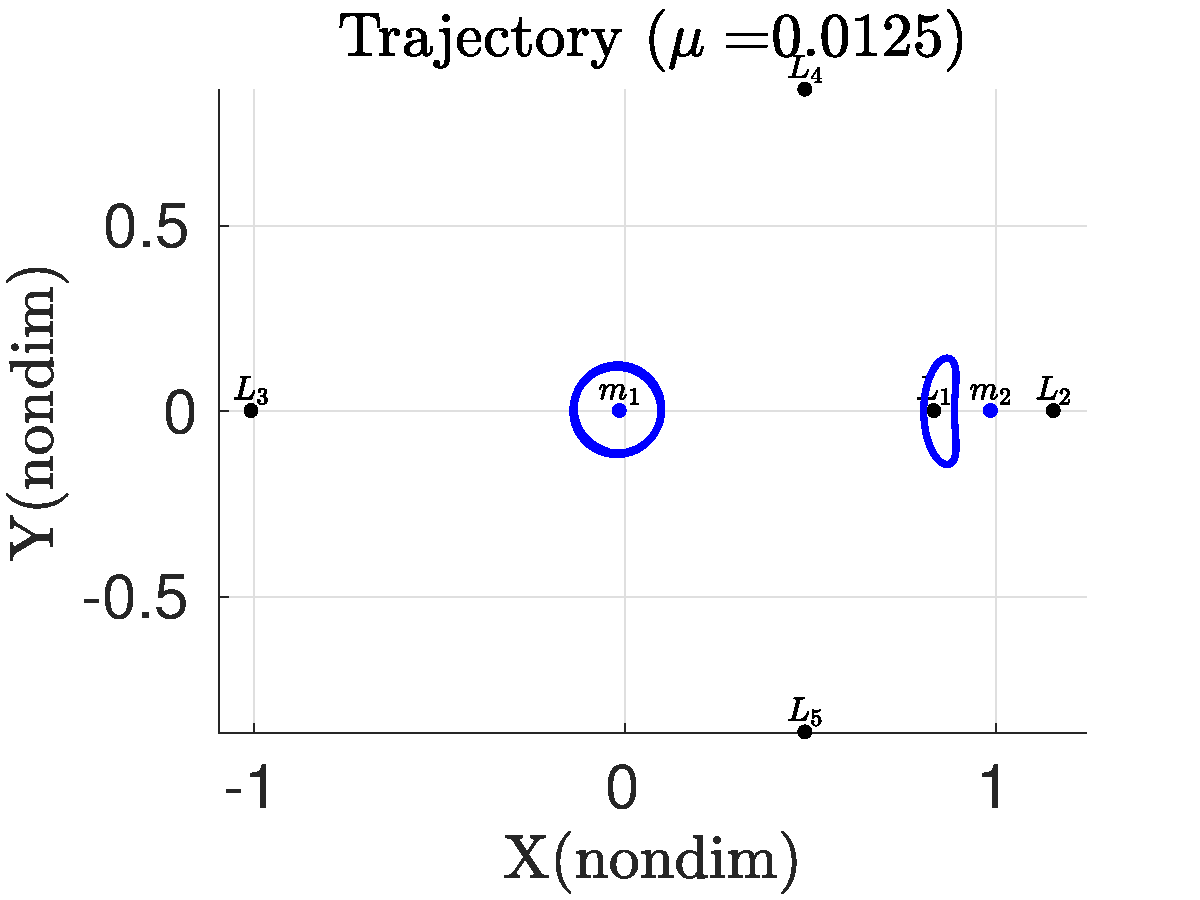
\includegraphics[width=0.5\textwidth]{figures/2017_JAS/initial_final} % requires the graphicx package
   \caption{Geostationary to \( L_1 \) transfer: Representation of the initial and target orbits for the reachability transfer. 
   Vehicle is assumed to begin on the geostationary orbit about \( m_1\) and will transfer to the periodic orbit about \( L_1\)}
   \label{fig:geo_transfer_target}
\end{figure}
In~\cref{fig:geo_transfer_target}, the initial orbit is located in the center of the figure and centered about \( m_1 \) while the target periodic orbit is determined about the \( L_1 \) Lagrange point.
Instead of determining a transfer directly between the geostationary orbit and the periodic orbit, we seek to instead transfer to the stable manifold of the periodic orbit.
This stable manifold will then asymptotically approach the target orbit without any further control input.
Once on the manifold, the spacecraft will coast in an uncontrolled fashion and asymptotically arrive at the desired periodic orbit.

We first generate the stable invariant manifold associated with the periodic orbit in order to determine our target set.
The stable manifold is propagated to the \Poincare section at \( y = 0 \), which is denoted by the horizontal black line in the position space visualizations given in~\cref{fig:stage1to4_reachability,fig:stage5to8_reachability,fig:geo_transfer_full}.
The stable manifold is denoted by the green trajectories which span the majority of the phase space. 
In addition, we plot the intersection of the stable manifold with the \Poincare section with green markers.
The initial orbit and the stable invariant manifold do not intersect and the transfer objective is to enlarge the reachability set to include the stable manifold.

Next, we compute the reachable sets originating on the geo-stationary orbit and subject to the maximum control constraint. 
The multiple shooting approach is used to solve the optimal control problem with two segments.
For the first reachability set computation, the initial geostationary orbit is used to initialize the multiple shooting algorithm.
We use the same initial guess of \( \vc{\lambda}_0\) as in~\cref{sec:periodic_orbit_transfer} and propagate over the fixed time horizon of the period of the geostationary orbit to initialize \( \vc{\lambda}_i^{-}\).

\begin{figure}[htbp]
    \centering
    \begin{subfigure}[htbp]{0.5\textwidth} 
        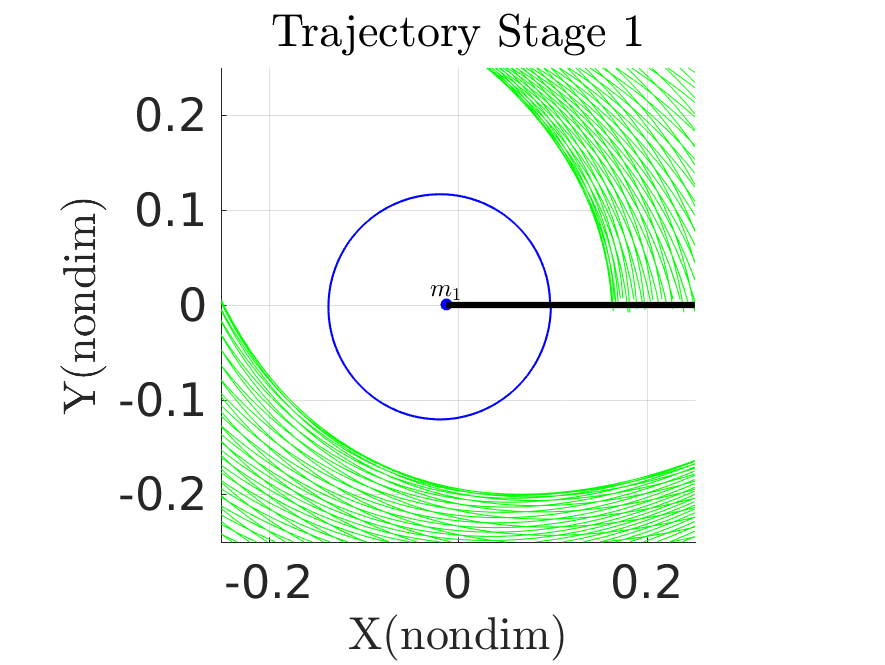
\includegraphics[width=\textwidth, keepaspectratio]{figures/2017_JAS/stage1_trajectory_zoom.pdf} 
        \caption{Stage 1 Trajectory~\label{fig:stage1_trajecotry_zoom}} 
    \end{subfigure}~
    \begin{subfigure}[htbp]{0.5\textwidth} 
        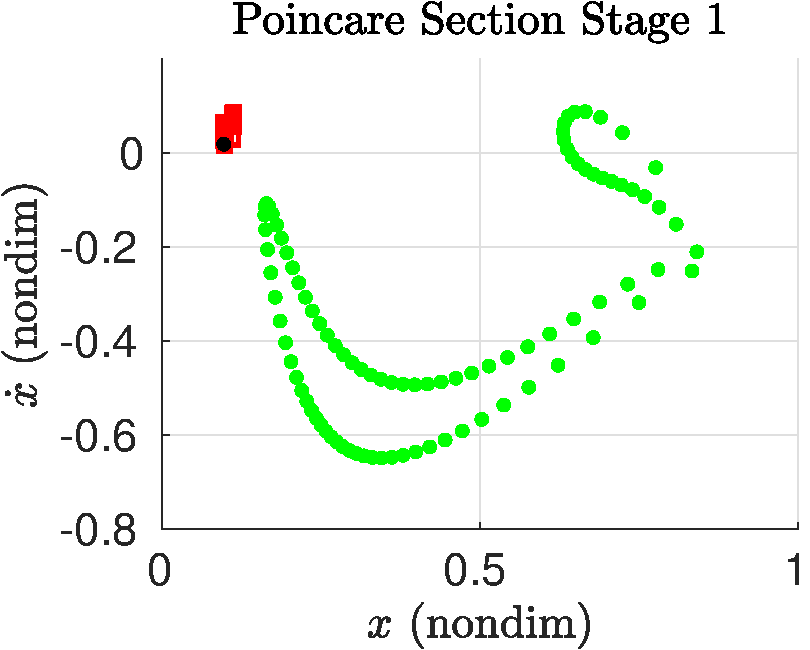
\includegraphics[width=\textwidth, keepaspectratio]{figures/2017_JAS/stage1_poincare.pdf} 
        \caption{Stage 1 \Poincare~section \label{fig:stage1_poincare}} 
    \end{subfigure}


    \begin{subfigure}[htbp]{0.5\textwidth} 
        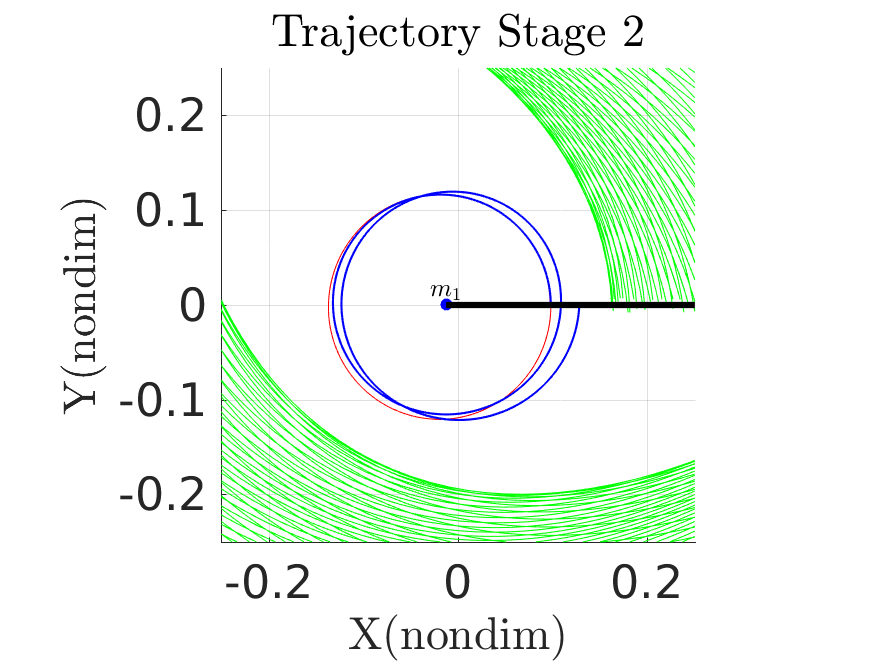
\includegraphics[width=\textwidth, keepaspectratio]{figures/2017_JAS/stage2_trajectory_zoom.pdf} 
        \caption{Stage 2 Trajectory~\label{fig:stage2_trajecotry_zoom}} 
    \end{subfigure}~
    \begin{subfigure}[htbp]{0.5\textwidth} 
        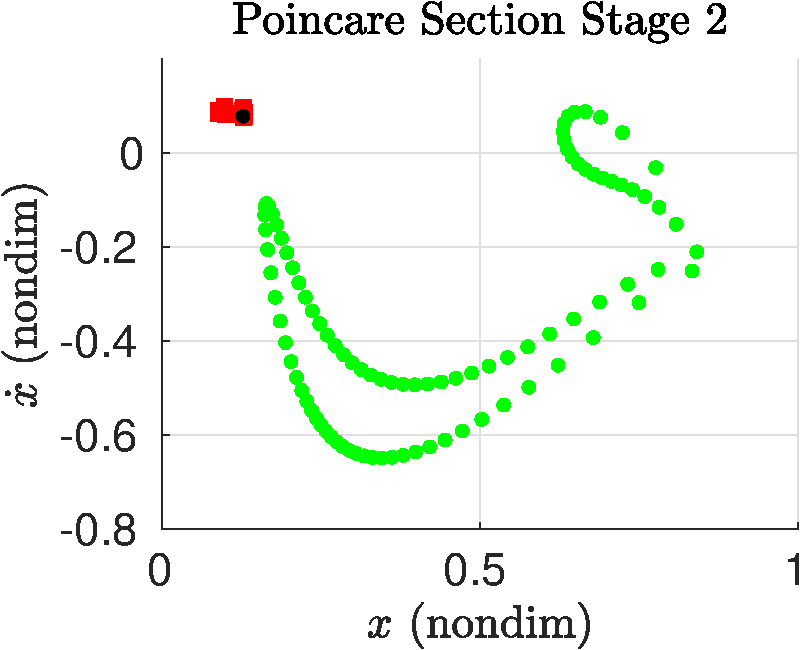
\includegraphics[width=\textwidth, keepaspectratio]{figures/2017_JAS/stage2_poincare.pdf} 
        \caption{Stage 2 \Poincare~section \label{fig:stage2_poincare}} 
    \end{subfigure}

    \begin{subfigure}[htbp]{0.5\textwidth} 
        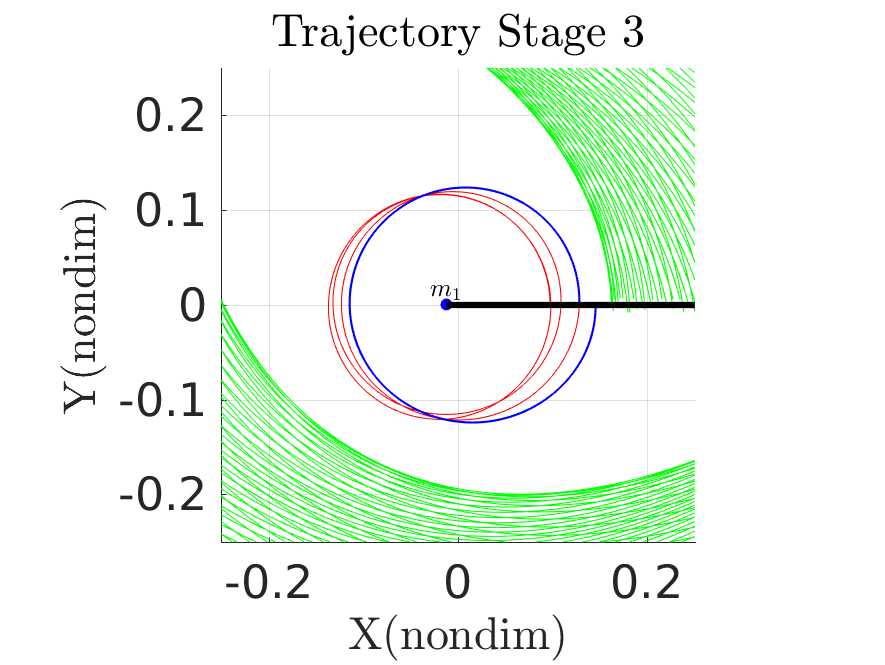
\includegraphics[width=\textwidth, keepaspectratio]{figures/2017_JAS/stage3_trajectory_zoom.pdf} 
        \caption{Stage 3 Trajectory~\label{fig:stage3_trajecotry_zoom}} 
    \end{subfigure}~
    \begin{subfigure}[htbp]{0.5\textwidth} 
        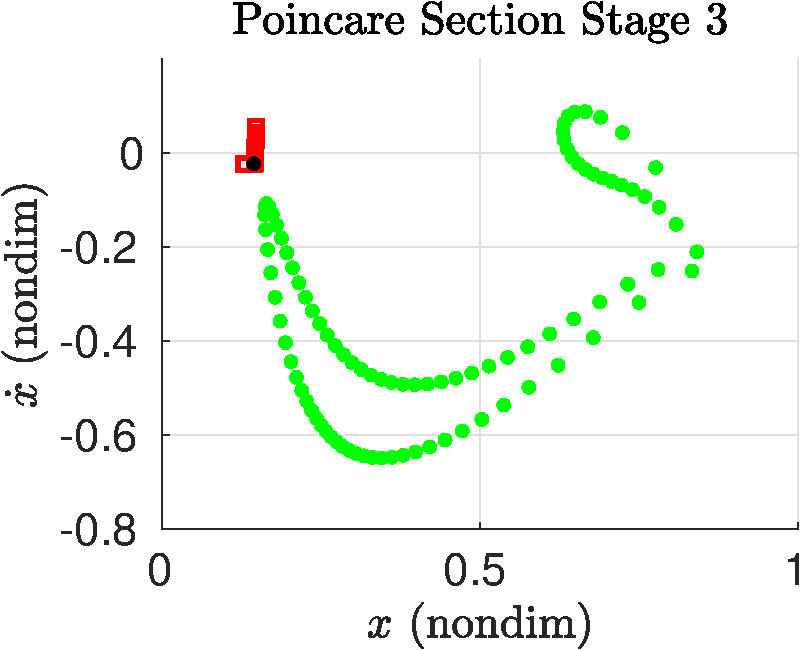
\includegraphics[width=\textwidth, keepaspectratio]{figures/2017_JAS/stage3_poincare.pdf} 
        \caption{Stage 3 \Poincare~section \label{fig:stage3_poincare}} 
    \end{subfigure}
 
    \begin{subfigure}[htbp]{0.5\textwidth} 
        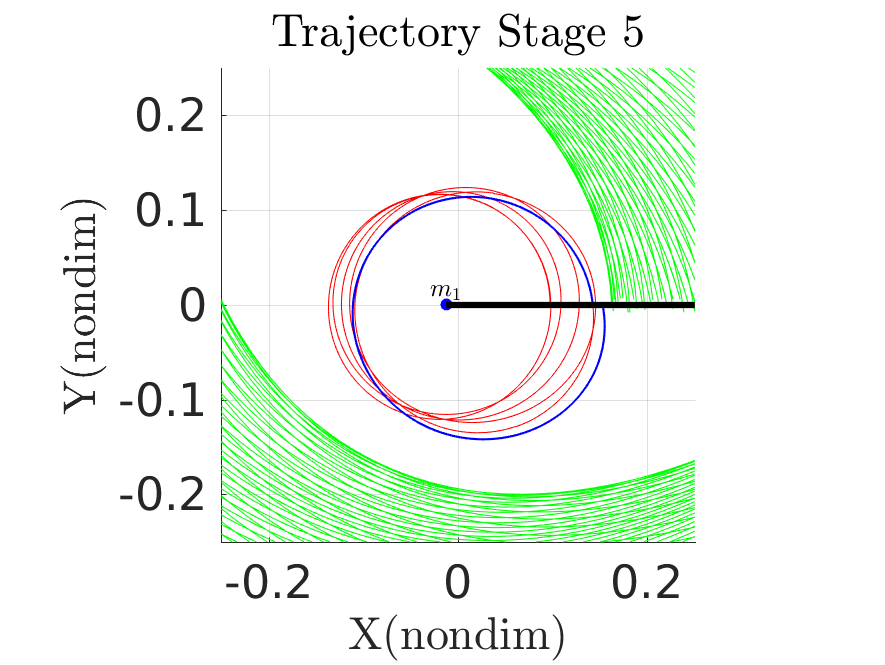
\includegraphics[width=\textwidth, keepaspectratio]{figures/2017_JAS/stage5_trajectory_zoom.pdf} 
        \caption{Stage 4 Trajectory~\label{fig:stage4_trajecotry_zoom}} 
    \end{subfigure}~
    \begin{subfigure}[htbp]{0.5\textwidth} 
        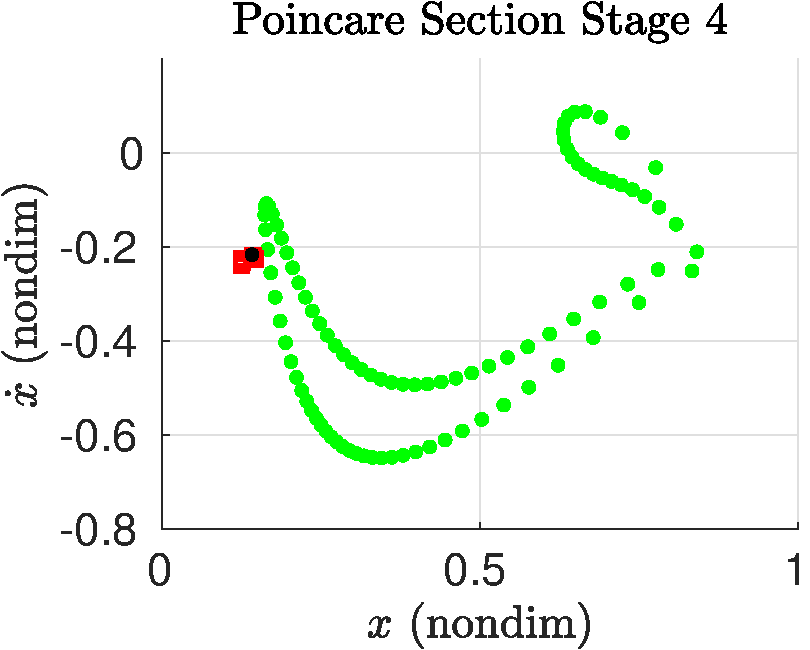
\includegraphics[width=\textwidth, keepaspectratio]{figures/2017_JAS/stage4_poincare.pdf} 
        \caption{Stage 4 \Poincare~section \label{fig:stage4_poincare}} 
    \end{subfigure}   
    \caption{Stage 1-4 reachability sets: The first four reachability sets visualized in both the position (left) and \Poincare space (right).
        The minimum trajectories from the preceding stages are shown in red, while the next stage is shown in blue.
    The transfer goal is to generate a complete trajectory from the initial geostationary orbit to the \( L_1 \) stable manifold, with an eventual arrival at the \( L_1 \) periodic orbit~\label{fig:stage1to4_reachability}}
\end{figure}
The first reachable set is computed beginning on the geostationary orbit at it's intersection with the \Poincare section and we again assume a upper bound on the thrust magnitude of \( u_{max} = 0.75 \).
The reachable set is generated by varying the angle \( \ang{0} \leq \theta < \ang{360} \) in~\cref{eq:constraints} defined on the \Poincare section.
This allows us to approximate the set of states that are achievable in the \( \parenth{x ,\dot{x}} \) space.
The intersection of the first reachable set with the \Poincare section is shown in~\cref{fig:stage1_poincare} in red.
While the reachable set does not intersect the stable manifold, it does reduce some of the distance in the \(\dot{x}\) dimension.
From this reachable set, we chose a trajectory which minimizes the distance towards the stable manifold, which is shown in~\cref{fig:stage1_poincare} by the black marker.
The distance on the \Poincare section between the reachable set and the stable manifolds is defined as the function \( d \),
\begin{align*}
        d(\vc{x}(N)) = \sqrt{\parenth{x - x_t}^2 + \parenth{\dot{x} - \dot{x}_t}^2}.
\end{align*}
From the reachable set, the trajectory which minimizes \( d \) is used to initialize the next iteration.
The minimum trajectory is also shown in~\cref{fig:stage1_trajecotry_zoom} and is used to initialize the following stage.
Over the relatively short time horizon of the geostationary orbital period, the reachability set remains quite close to the initial orbit. 
However, the addition of the control input has increased the velocity component of the trajectory.
It is this velocity change that is subsequently exploited to generate the transfer trajectory.

The minimum trajectory from the first iteration of the reachability set is used to initialize the following stage.
From the terminal state of the first iteration, the second reachability set is computed and displayed in~\cref{fig:stage2_trajecotry_zoom,fig:stage2_poincare}.
The second reachability set is shown on the \Poincare section in~\cref{fig:stage2_poincare}.
This iteration greatly decreases the distance in the \( x \) component between the trajectory and the target, at the expense of a small deviation in the \( \dot{x} \) component.
In~\cref{fig:stage2_trajecotry_zoom}, the first stage trajectory is shown in red while the additional stage is shown in blue, which demonstrates the decrease in the \( x \) component.

\begin{figure}[htbp]
    \centering
    \begin{subfigure}[htbp]{0.5\textwidth} 
        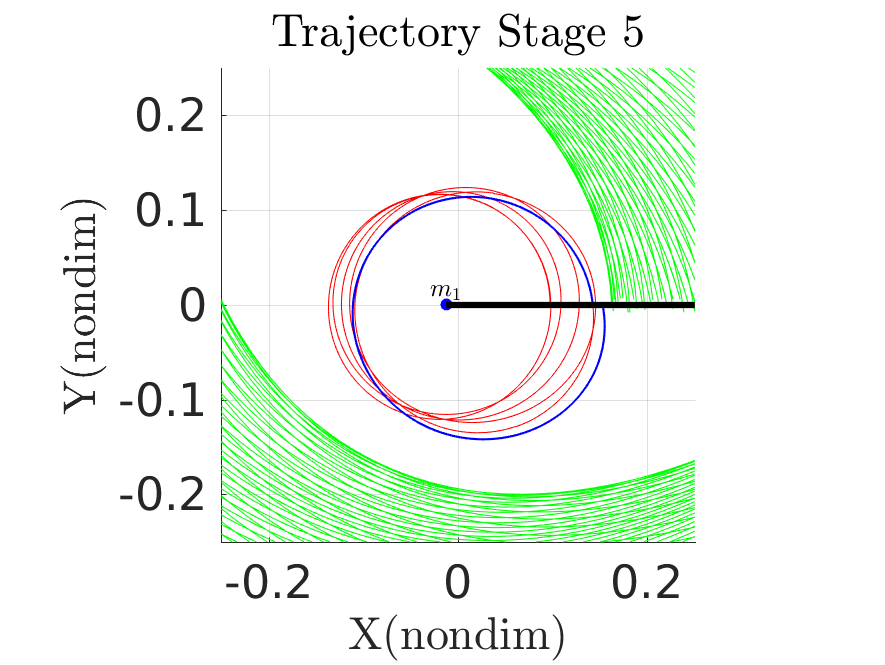
\includegraphics[width=\textwidth, keepaspectratio]{figures/2017_JAS/stage5_trajectory_zoom.pdf} 
        \caption{Stage 5 Trajectory~\label{fig:stage5_trajecotry_zoom}} 
    \end{subfigure}~
    \begin{subfigure}[htbp]{0.5\textwidth} 
        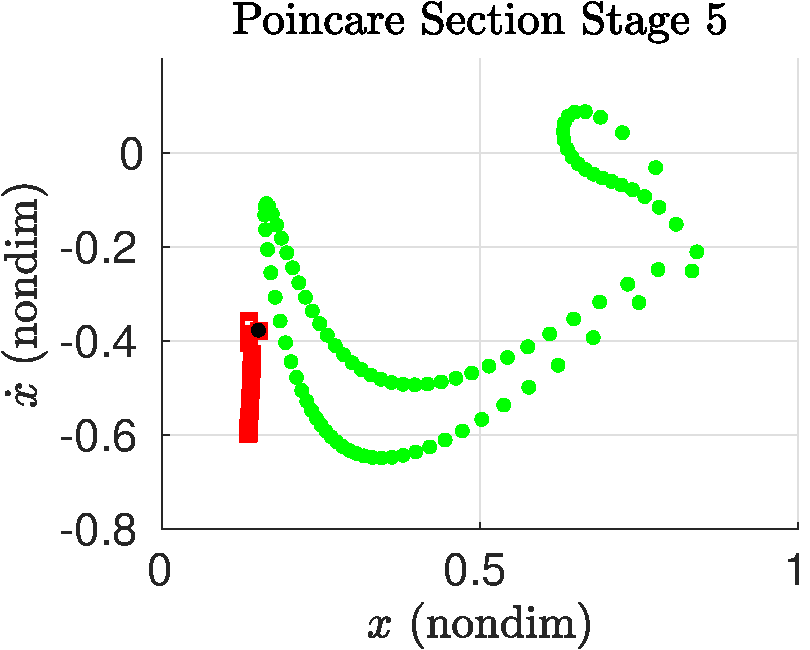
\includegraphics[width=\textwidth, keepaspectratio]{figures/2017_JAS/stage5_poincare.pdf} 
        \caption{Stage 5 \Poincare~section \label{fig:stage5_poincare}} 
    \end{subfigure}

    \begin{subfigure}[htbp]{0.5\textwidth} 
        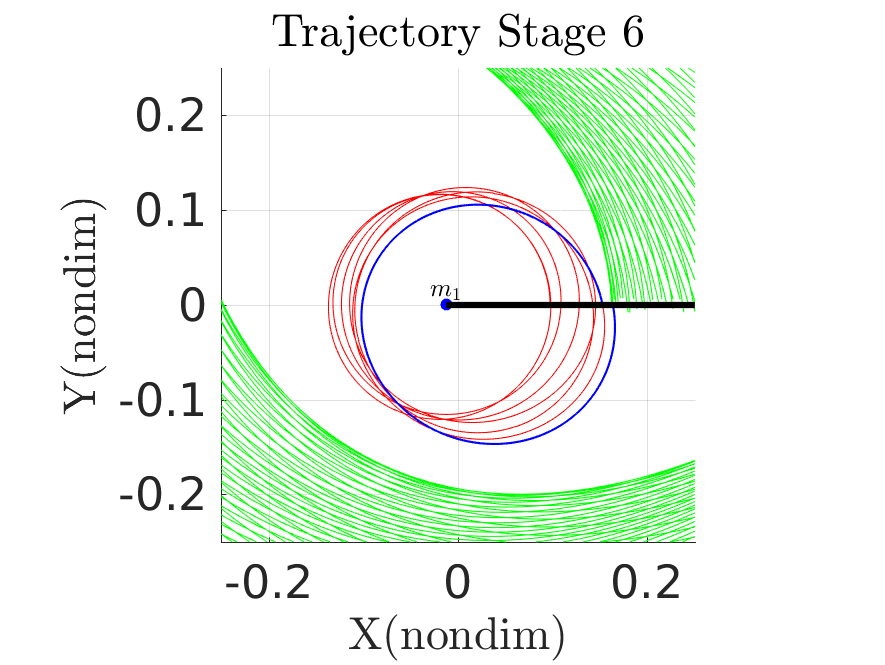
\includegraphics[width=\textwidth, keepaspectratio]{figures/2017_JAS/stage6_trajectory_zoom.pdf} 
        \caption{Stage 6 Trajectory~\label{fig:stage6_trajecotry_zoom}} 
    \end{subfigure}~
    \begin{subfigure}[htbp]{0.5\textwidth} 
        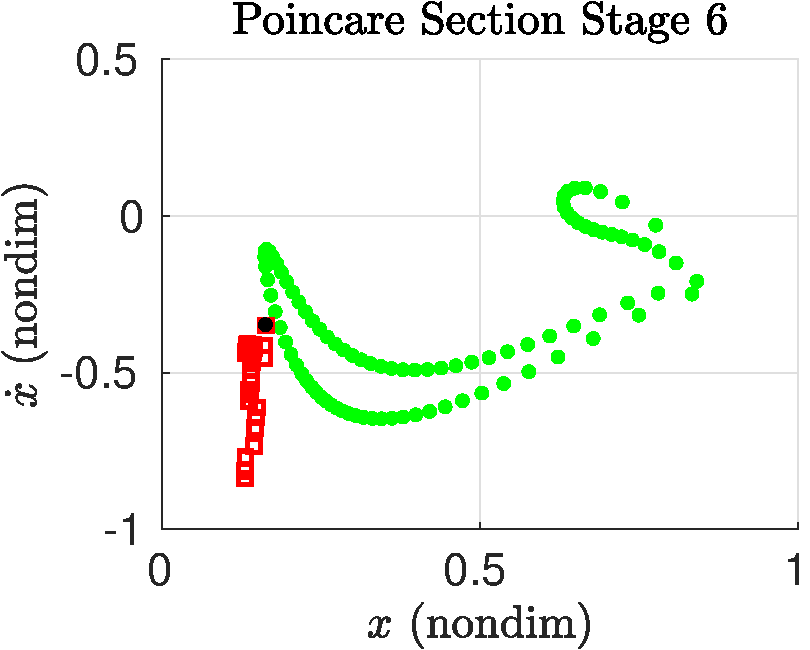
\includegraphics[width=\textwidth, keepaspectratio]{figures/2017_JAS/stage6_poincare.pdf} 
        \caption{Stage 6 \Poincare~section \label{fig:stage6_poincare}} 
    \end{subfigure}

    \begin{subfigure}[htbp]{0.5\textwidth} 
        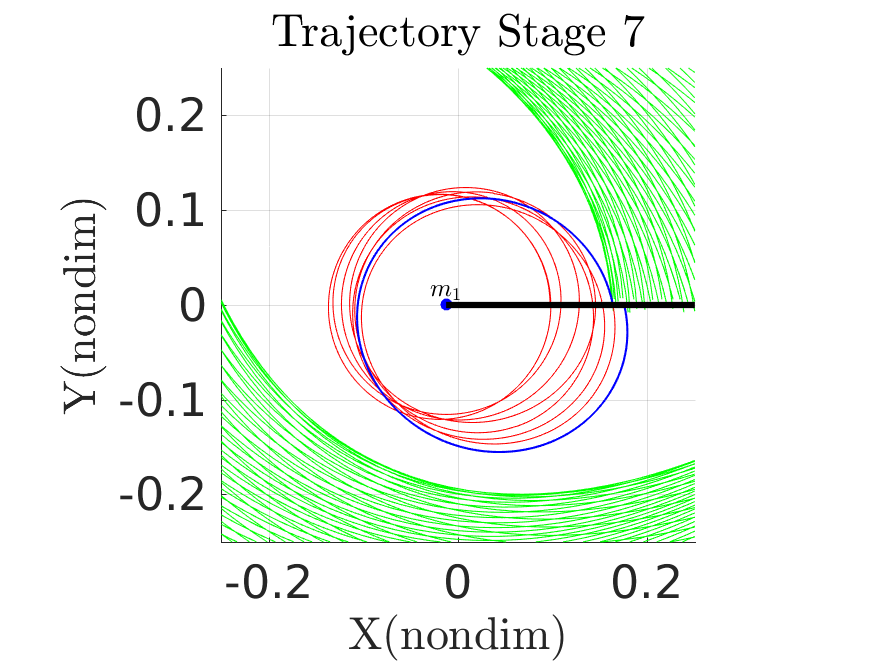
\includegraphics[width=\textwidth, keepaspectratio]{figures/2017_JAS/stage7_trajectory_zoom.pdf} 
        \caption{Stage 7 Trajectory~\label{fig:stage7_trajecotry_zoom}} 
    \end{subfigure}~
    \begin{subfigure}[htbp]{0.5\textwidth} 
        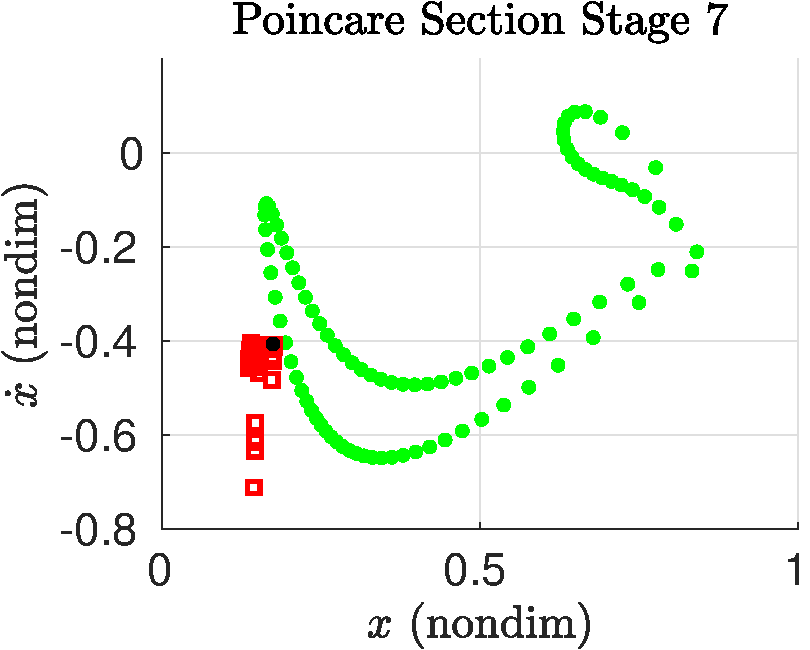
\includegraphics[width=\textwidth, keepaspectratio]{figures/2017_JAS/stage7_poincare.pdf} 
        \caption{Stage 7 \Poincare~section \label{fig:stage7_poincare}} 
    \end{subfigure}
 
    \begin{subfigure}[htbp]{0.5\textwidth} 
        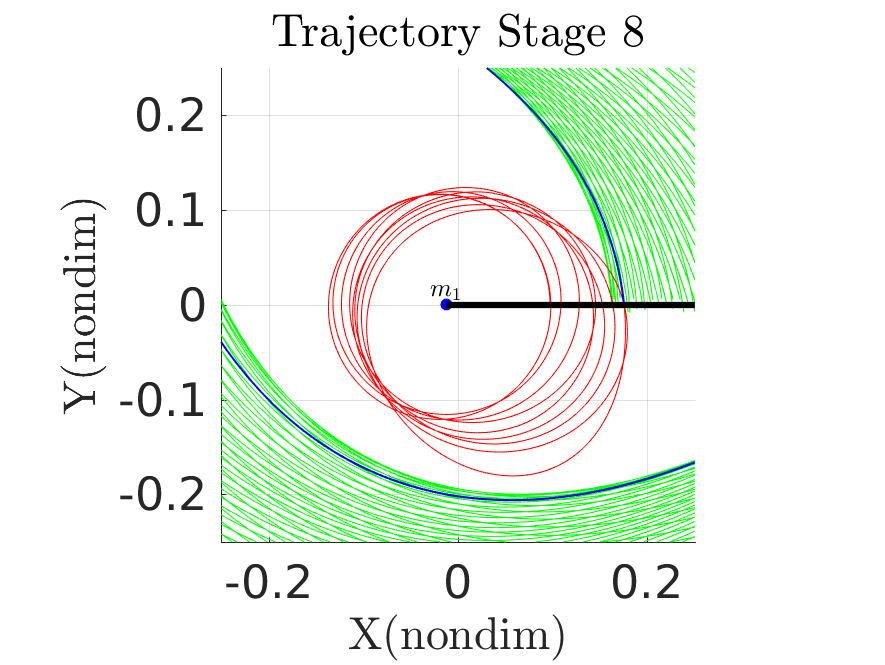
\includegraphics[width=\textwidth, keepaspectratio]{figures/2017_JAS/stage8_trajectory_zoom.pdf} 
        \caption{Stage 8 Trajectory~\label{fig:stage8_trajecotry_zoom}} 
    \end{subfigure}~
    \begin{subfigure}[htbp]{0.5\textwidth} 
        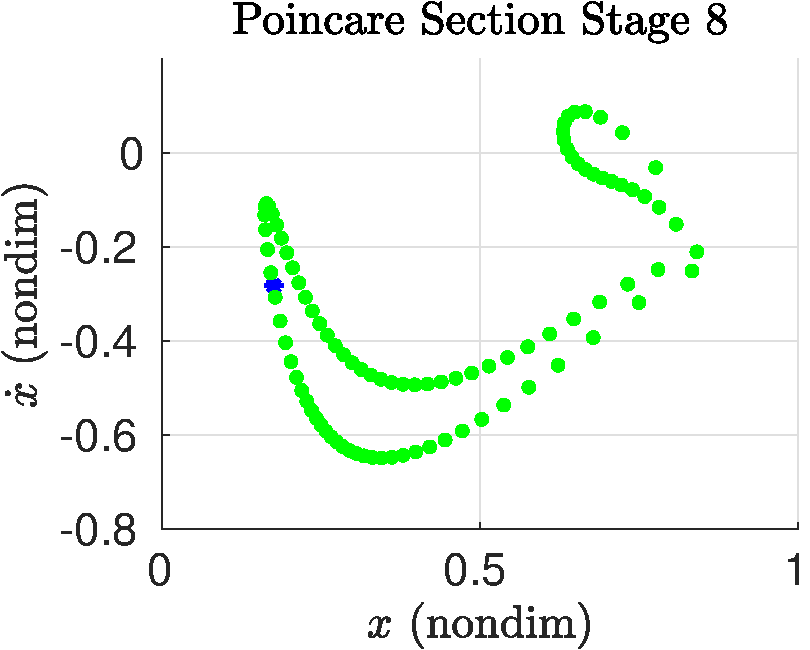
\includegraphics[width=\textwidth, keepaspectratio]{figures/2017_JAS/stage8_poincare.pdf} 
        \caption{Stage 8 \Poincare~section \label{fig:stage8_poincare}} 
    \end{subfigure}   
    \caption{Stage 5-8 reachability sets: The last four reachability sets visualized in both the position (left) and \Poincare space (right).
        The minimum trajectories from the preceding stages are shown in red, while the next stage is shown in blue.
    The transfer goal is to generate a complete trajectory from the initial geostationary orbit to the \( L_1 \) stable manifold, with an eventual arrival at the \( L_1 \) periodic orbit~\label{fig:stage5to8_reachability}}
\end{figure}

With each reachable set we move the controlled trajectory closer to the target stable manifold.
\Cref{fig:stage1to4_reachability,fig:stage5to8_reachability} shows all of the intermediate reachability iterations to transfer between the initial orbit and the stable invariant manifold.
The final reachable set intersects the stable manifold of the periodic orbit. 
A final fixed terminal time and terminal state optimal transfer is finally used to arrive at the stable manifold.
The optimization statistics for the final transfer are shown in~\cref{tab:geo_transfer}.
\begin{table}[h]
    \centering
    \begin{tabular}{llr}  
        \toprule
        Metric    & Value \\
        \midrule
        \texttt{fsolve} objective      & \num{1.42e-11}      \\
        \texttt{fsolve} major iterations       & \num{18}      \\
        \texttt{fsolve} first order optimality & \num{7.2e-11} \\
        Optimal cost       & \num{4.30e-25}      \\
        Execution time & \SI{2.62}{\second}       \\
        \bottomrule
    \end{tabular}
    \caption{Convergence statistics for the geostationary orbit transfer\label{tab:geo_transfer}}
\end{table}
The complete transfer trajectory, after eight iterations, is shown in~\Cref{fig:geo_transfer}. 
Combining these trajectories results in the powered portion of the transfer from the geostationary orbit to the stable manifold. 
Each iteration systematically moves the reachable set towards the stable manifold. 
Furthermore, the optimal control formulation is simplified as each iteration is initialized using a simple distance metric on the \Poincare section.
\Cref{fig:geo_transfer_full,fig:geo_transfer_zoom} shows the resulting trajectory, with the final trajectory shown in red which ensures the intersection with the stable invariant manifold.
\Cref{fig:geo_transfer_poincare} shows the \Poincare section with the minimum reachable state from each iteration.
Each iteration seeks to decrease the distance to the stable manifold on the \Poincare section.
Furthermore, these minimum states serve to initialize each subsequent stage of the transfer. 
This method provides a systematic and simple methodology to determine transfer trajectories.
Instead of relying purely on numerical optimization to find an appropriate trajectory, our method instead utilizes the reachability set to determine suitable trajectories.
Once at the stable manifold, no further control input is required and the vehicle will coast towards the target periodic orbit.
\Cref{fig:control_input_geo} shows the control input during the powered portion of the transfer. 
We utilize the same spacecraft assumption of \SI{500}{\kilo\gram} from~\cref{sec:periodic_orbit_transfer} which gives a maximum thrust of approximately \SI{1}{\newton}.
The spacecraft maintains a bounded control magnitude during the transfer to the stable manifold.
\Cref{fig:jacobi_geo} shows the evolution of the Jacobi energy over the transfer.
Each stage of the transfer serves to raise the energy level of the vehicle.
After eight stages the reachability set intersects the stable manifold and a demonstrates that a transfer is achievable.
The final optimal control drives the vehicle towards the target manifold with the appropriate energy level.
\begin{figure} 
        \centering 
        \subcaptionbox{Transfer trajectory: Complete trajectory consisting of eight iterations (1-7 black and final in red) of the reachability sets with a final control-free coast (blue)  on the stable manifold (green).\label{fig:geo_transfer_full}}{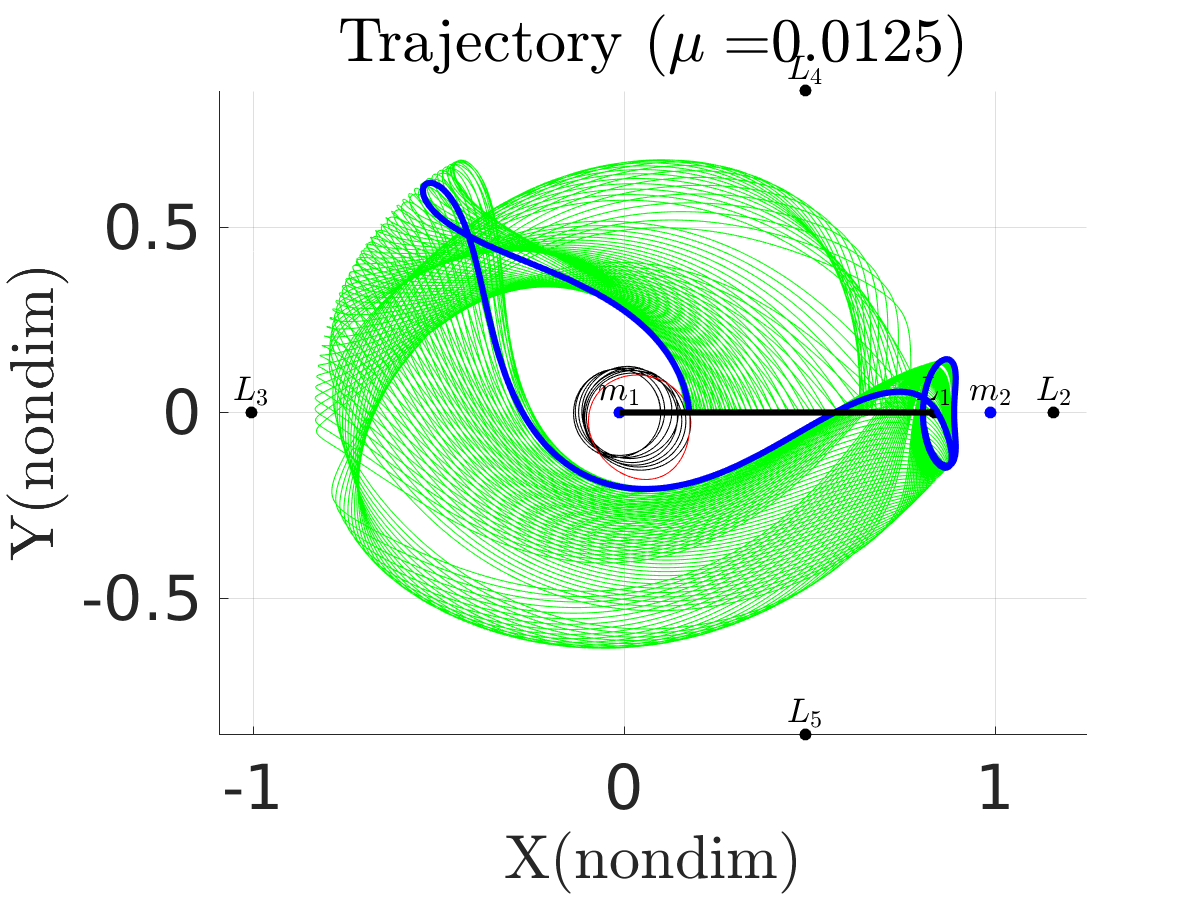
\includegraphics[width=0.45\textwidth]{figures/2017_JAS/geo_transfer_full}}\hfill
        \subcaptionbox{Detailed view of transfer: Centered at \(m_1\) the eight
            iterations from the reachability analysis are shown in black.  The
            final segment to the stable manifold is shown in red.  Each
            iteration progressively approaches the stable manifold.  Once on
        the stable manifold the vehicle can coast without thrust towards the
    periodic orbit.\label{fig:geo_transfer_zoom}
}{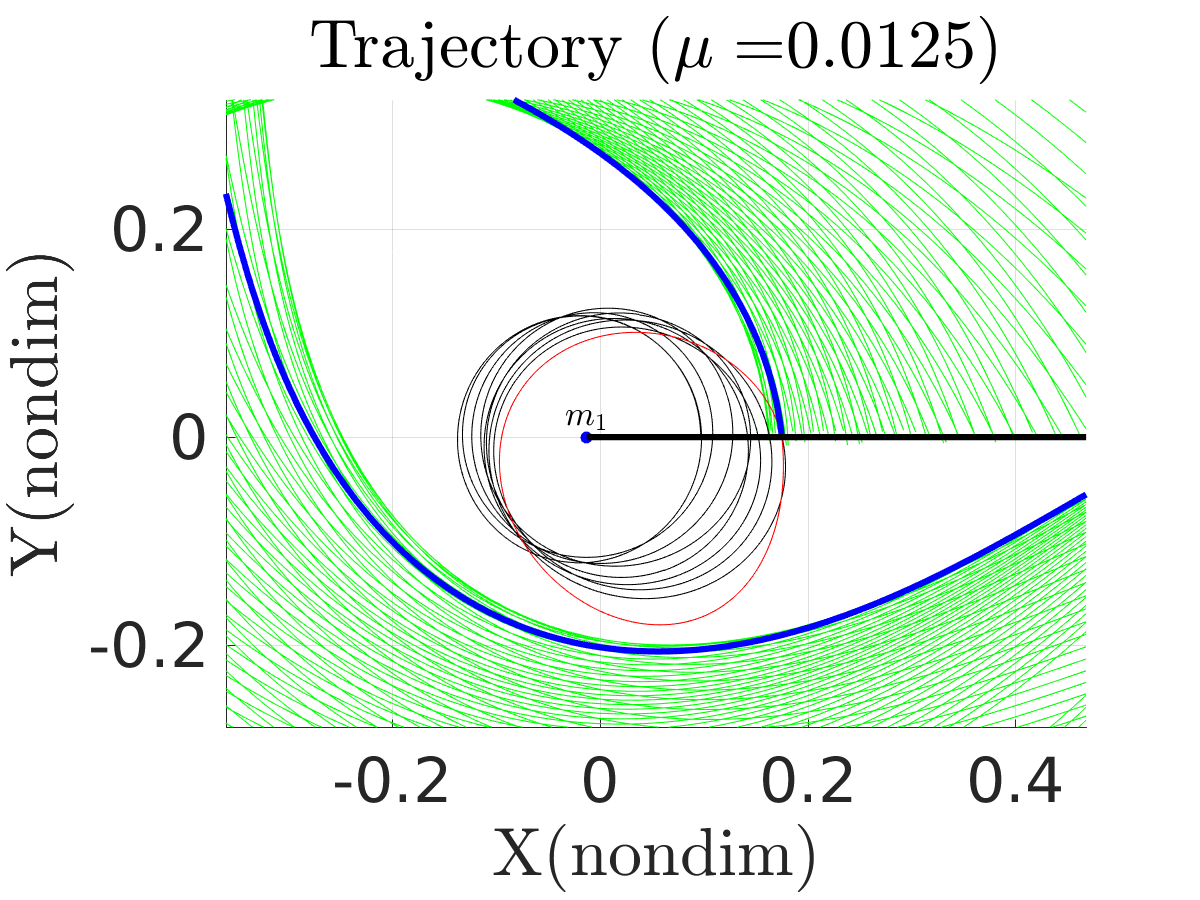
\includegraphics[width=0.45\textwidth]{figures/2017_JAS/geo_transfer_zoom}}
       
\subcaptionbox{\Poincare section: Minimum distance states from each iteration of the reachability set analysis (red) with respect to the stable invariant manifold (green)\label{fig:geo_transfer_poincare}}{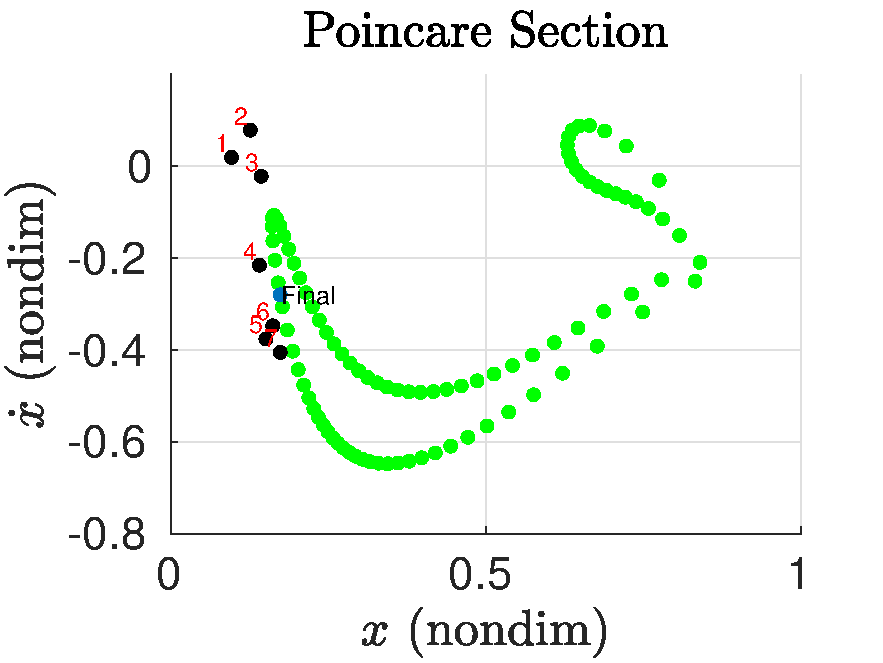
\includegraphics[width=0.45\textwidth]{figures/2017_JAS/poincare}}
    \hfill
    \subcaptionbox{Control Input: Combined control history for each stage of the reachability analysis. 
    The control always remains within the maximum bound.\label{fig:control_input_geo}}{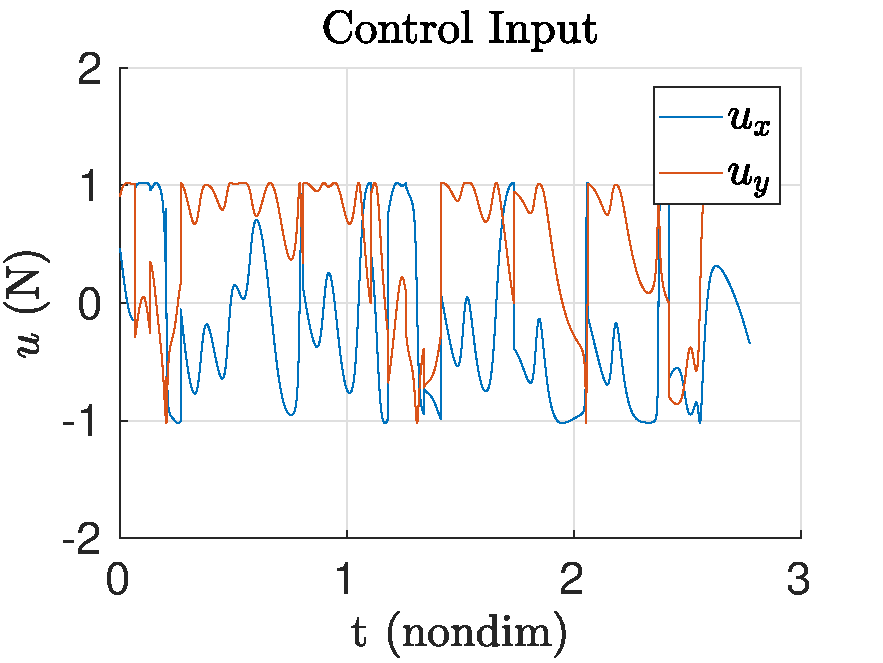
\includegraphics[width=0.45\textwidth]{figures/2017_JAS/control_input_geo.pdf}}

    \subcaptionbox{Jacobi Energy: Energy history throughout the transfer.
    Each stage of the transfer serves to increase the energy towards the stable manifold. 
The final reachability set intersects the stable manifold and enables a large final maneuver to the target orbit.\label{fig:jacobi_geo}}{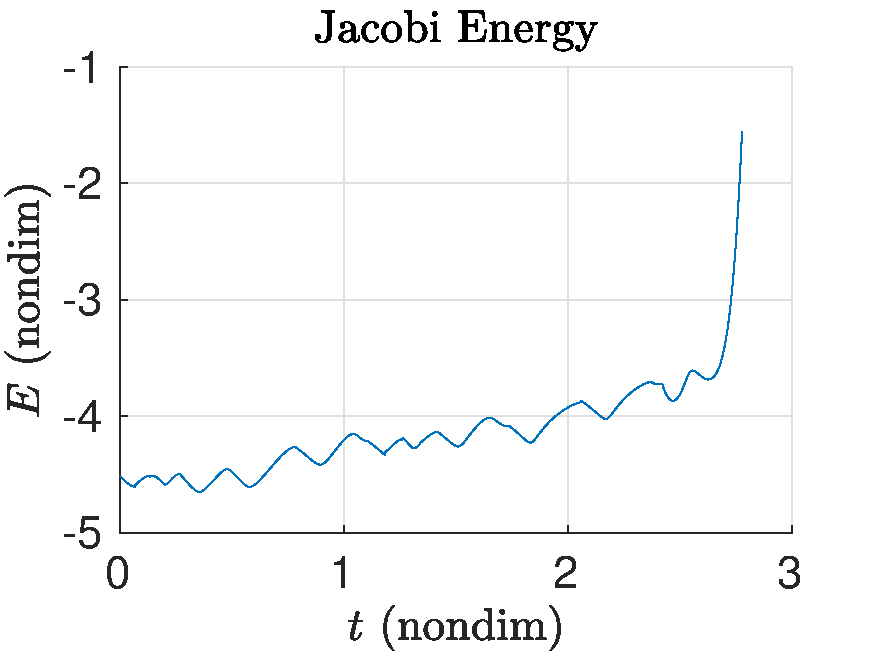
\includegraphics[width=0.5\textwidth]{figures/2017_JAS/jacobi_energy.pdf}}

        \caption{Geostationary to \( L_1 \) periodic orbit transfer: Complete transfer from the geostationary orbit to the stable manifold.\label{fig:geo_transfer}}
\end{figure}

This numerical example demonstrates the ability to link several computations of the reachability set to enable a more general transfer.
We use eight iterations of computing the reachability set in order to transfer from the geostationary orbit to the stable manifold.
This approach allows for a larger class of potential transfers which leverage the capabilities of low-thrust propulsion systems.
We are able to achieve a transfer that is not possible via the standard invariant manifold approach. 
In addition, this example illustrates a straightforward method to depart from the natural dynamics and transfer to a large region of the phase space that is not accessible via invariant manifolds alone.
\subsection{4769 Castalia Examples}\label{sec:castalia_transfer}
In this section, we extend the results developed in the planar three body problem to the higher dimensional space around an asteroid.
As shown in~\cref{sec:sc_eoms}, the translational dynamics of a point mass around an asteroid asteroid are similar to that of the three body problem.
Similar to~\cref{sec:periodic_orbit_transfer}, a \Poincare section is defined and the reachability set is approximated on this space. 
This lower dimensional space is used to design a transfer trajectory to move the vehicle between equatorial orbits of asteroid Castalia.

We apply the \Poincare map with a surface of section chosen to be normal to the position \( y = 0 \).
The \Poincare map is then defined as the map between successive transversal crossings of the surface of section.
To ensure a transverse crossing of the section we also require that \( \dot{y} \neq 0 \) when \( y = 0 \).
With this definition of the \Poincare map, it is possible to remove the two variables \( y \) and \( \dot{y} \) from consideration and create a four-dimensional map from the \Poincare section to itself.
The \Poincare section, represented by \( \Sigma \), then becomes
\begin{align}\label{eq:poincare_section}
    \Sigma = \braces{\parenth{x, \dot{x}, z, \dot{z}} | y(t_f) = 0 }.
\end{align}
We use this section to compute periodic orbits that serve as the initial and target states of our transfer.
In addition, this section serves as a lower dimensional space upon which we approximate the reachability set.

The cost function is given by~\cref{eq:cost}, but modified for the extra dimensions in this problem.
We use the matrix \( Q = \text{diag} \bracket{1~\>0~\> 1~\> 1~\>0~\>1 } \in \R^{6 \times 6}\) to represent the mapping onto \( \Sigma \).
Maximization of the distance between \( \vc{x}_n \) and \(\vc{x} \), on the \Poincare section defined in~\cref{eq:poincare_section}, is equivalent to the minimization of \( J \) defined in~\cref{eq:cost}.
We ensure that the trajectories intersect the \Poincare section through the use of terminal constraints.
In addition, we use the terminal constraints to define a specific direction along which we seek to minimize the cost~\cref{eq:cost}.
Since the \Poincare section is four-dimensional, we parameterize a direction in \( \R^4 \)  using three angles \( \phi_1, \phi_2 , \phi_3 \).
The terminal constraints are given in terms of these angles as
\begin{align}\label{eq:terminal_constraints}
    \begin{split}
        m_1 &= y = 0 , \\
        m_2 &= \parenth{\sin \phi_{1_{d}}} \parenth{ x_1^2 + x_2^2 + x_3^2 + x_4^2} - x_1^2 = 0, \\
        m_3 &= \parenth{\sin \phi_{2_{d}}} \parenth{ x_2^2 + x_3^2 + x_4^2} - x_2^2 = 0, \\
        m_4 &= \parenth{\sin \phi_{3_{d}}} \parenth{ 2 x_3^2 + 2 x_3 \sqrt{x_4^2 + 2 x_4^2}} - x_3 - \sqrt{x_4^2 + x_3^2} = 0 ,
    \end{split}
\end{align}
where we make use of the difference states \( \parenth{x_1, x_2 ,x_3, x_4 }\) defined as
\begin{align}\label{eq:diff_states}
    \begin{split}
        x_1 &= x(t_f) - x_n(t_f) , \\
        x_2 &= z(t_f) - z_n(t_f) , \\
        x_3 &= \dot{x}(t_f) - \dot{x}_n(t_f) , \\
        x_4 &= \dot{z}(t_f) - \dot{z}_n(t_f) . \\
    \end{split}
\end{align}
We select the terminal time, \( t_f \), from the time required for the uncontrolled trajectory to return back to the \Poincare section.
The constraint \( m_1 = 0 \) ensures that the terminal state lies on the \Poincare section.
The constraints \( m_2, m_3, m_4 \) are used to define a direction on the \Poincare section.
\Cref{eq:diff_states} represents the difference between our controlled and uncontrolled trajectory on the \Poincare section.
We approximate the entire reachable set by discretization  over the space of angles \(\phi_1, \phi_2, \phi_3 \).
By convention we assume that the angles lie in the following range
\begin{align*}
    \phi_1, \phi_2 &\in [ 0, \pi ) ,\\
    \phi_3 &\in [ 0 , 2 \pi ) ,
\end{align*}
such that we parameterize all directions on the three sphere, \(\S^3\).
Finally, we also incorporate the control acceleration magnitude constraint as
\begin{align}\label{eq:control_constraint}
    c(\vc{u}) = \vc{u}^T \vc{u} - u_m^2 \leq 0 ,
\end{align}
where \( u_m \) is the maximum acceleration possible by the propulsion system.
This constraint assumes that the control acceleration may be orientated in any direction yet the acceleration magnitude is variable but bounded.
The goal is to determine the control history \( \vc{u}(t) \) such that the cost function~\cref{eq:cost} is minimized while subject to the equations of motion~\cref{eq:body_eoms} and the constraints~\cref{eq:control_constraint,eq:terminal_constraints}.

We present an example transfer of a spacecraft about the asteroid 4769 Castalia. 
Our equations of motion, given by~\cref{eq:eoms}, are an idealized version of the dynamics of a spacecraft.
For example, the model does not include the effect of mass transfer from propellant usage. 
We instead model the control input as a generic acceleration vector in the body-fixed asteroid frame. 
The acceleration magnitude constraint in~\cref{eq:control_constraint} is chosen to emulate a physically realizable thruster system.
In this analysis, we assume \( u_m = \SI{0.1}{\milli\meter\per\second\squared}\) which is equivalent to a thrust of approximately \SI{100}{\milli\newton} for a \SI{1000}{\kilo\gram} spacecraft.
This amount of thrust is typical of many current ion or hall effect thrusters~\cite{goebel2008,choueiri2009}.

The objective is to transfer the spacecraft between two periodic equatorial orbits about Castalia.
The initial and target orbits are periodic solutions about Castlia computed using the method introduced by Reference~\cite{scheeres2003}.
The initial conditions for both orbits are defined in the body-fixed frame as
\begin{align}\label{sec:initial_transfer}
    \vc{x}_i = 
    \begin{bmatrix}
        1.4973 \\ 0 \\ 0.0061 \\ 0\\ -0.0009 \\ 0
    \end{bmatrix} ,
    \quad
    \vc{x}_t =
    \begin{bmatrix}
        6.1175 \\ 0 \\ 0.0001 \\ 0\\ -0.0025 \\ 0
    \end{bmatrix} .
\end{align}
\Cref{fig:initial_transfer} shows the initial, \( \vc{x}_i \), and target, \( \vc{x}_t\), periodic orbits which lie in the equatorial plane of Castalia.
Our goal is to transfer from a lower altitude to a higher altitude while remaining in the equatorial plane of the asteroid.
This type of scenario would occur frequently during mapping and observation missions to asteroids.
\begin{figure}[htbp]
    \centering 
    \begin{subfigure}[htbp]{0.45\textwidth} 
        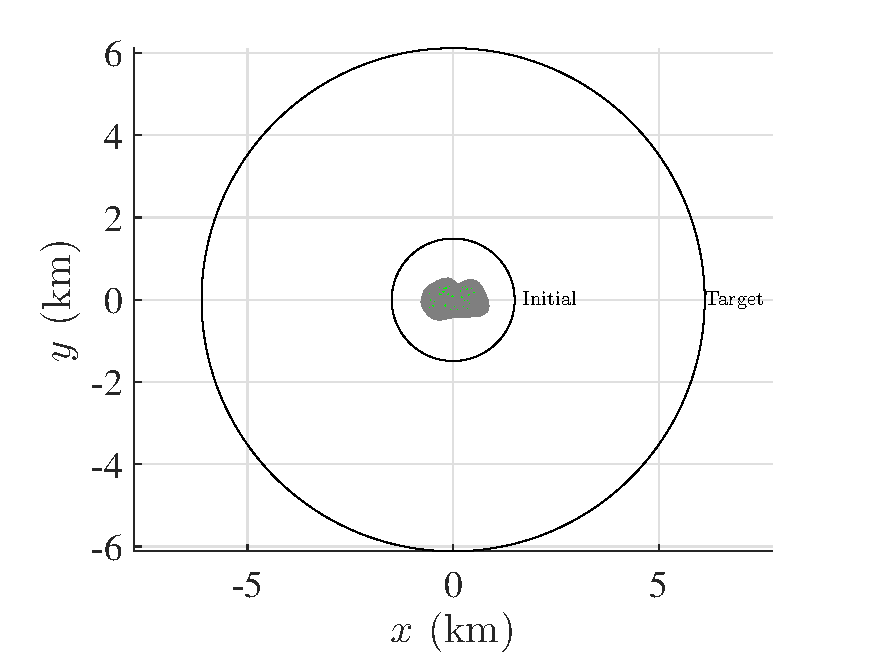
\includegraphics[width=\textwidth]{figures/2016_AAS/initial_transfer} 
        \caption{Equatorial View} \label{fig:eq_initial_transfer} 
    \end{subfigure}~ %add desired spacing between images, e. g. ~, \quad, \qquad, \hfill etc. %(or a blank line to force the subfigure onto a new line) 
    \begin{subfigure}[htbp]{0.45\textwidth} 
        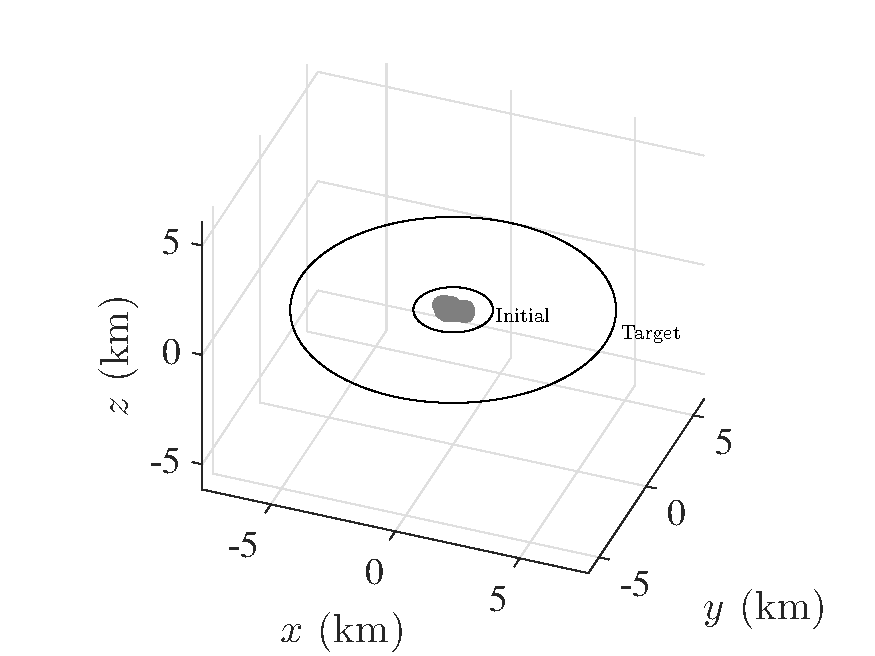
\includegraphics[width=\textwidth]{figures/2016_AAS/initial_transfer_3d} 
        \caption{3D view} \label{fig:initial_transfer_3d} 
    \end{subfigure} ~ %add desired spacing between images, e. g. ~, \quad, \qquad, \hfill etc. %(or a blank line to force the subfigure onto a new line) 
    \caption{Initial and target periodic orbits}
    \label{fig:initial_transfer} 
\end{figure}
In this transfer example we also have used a reduced model of Castalia.
Rather than using the full \num{4092} face model we reduce the number of faces to \num{1024} using the Matlab function \verb+reducepatch+. 
This greatly speeds up the computation with only a small difference in the gravitational field.

We first compute the reachability set originating from the initial periodic orbit at \( \vecbf{x}_i\) for a fixed time of flight and bounded control magnitude as defined previously.
The reachability set is computed by solving the two-point boundary value problem using a multiple shooting algorithm to satisfy the necessary conditions in~\cref{eq:necc_conditions}.
The reachability set is generated on the lower dimensional \Poincare section and is composed of the terminal states in the \( \parenth{x,z,\dot{x},\dot{z} } \) space.
We approximate the reachability set by discretization of each of the angles \( \phi_1, \phi_2 , \phi_3 \) into ten discrete steps. 
This results in a total of \(10^3\) trajectories which approximate the reachability set on the \Poincare section.

We visualize the section using the two figures in~\cref{fig:poincare_section}.
\begin{figure}[htbp]
    \centering 
    \begin{subfigure}[htbp]{0.45\textwidth} 
        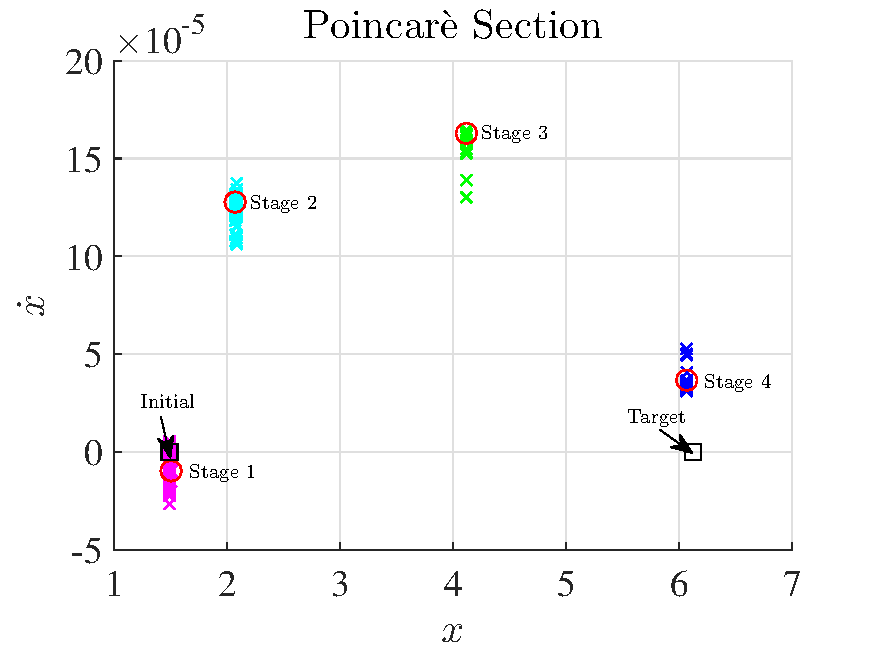
\includegraphics[width=\textwidth]{figures/2016_AAS/poincare_xvsxdot.pdf} 
        \caption{\( x \) vs. \( \dot{x} \) \Poincare section} \label{fig:poincare_xvsxdot} 
    \end{subfigure}~
    \begin{subfigure}[htbp]{0.45\textwidth} 
        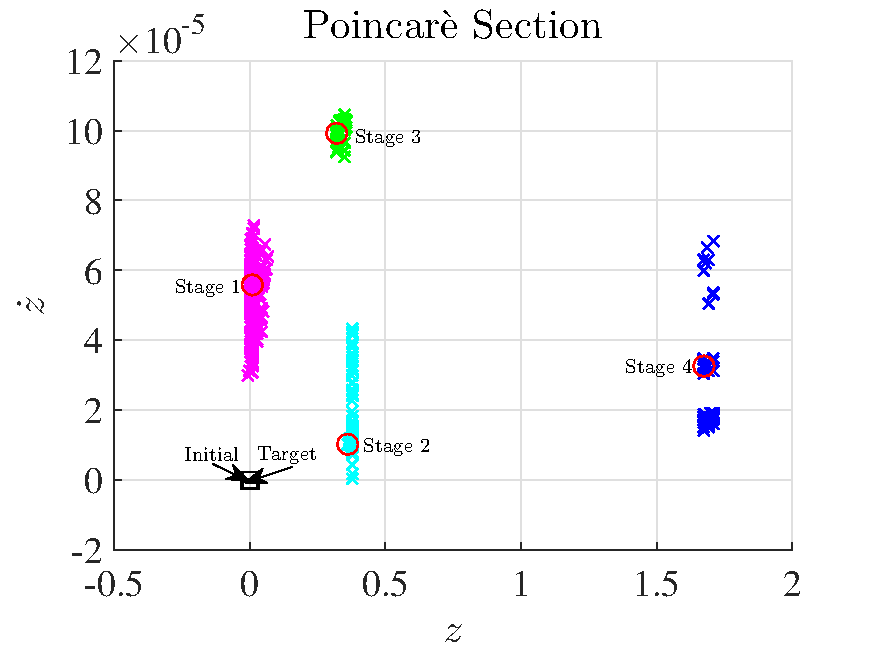
\includegraphics[width=\textwidth]{figures/2016_AAS/poincare_zvszdot.pdf} 
        \caption{\( z \) vs. \( \dot{z} \) \Poincare section} \label{fig:poincare_zvszdot} 
    \end{subfigure}
    \caption{\Poincare section visualization \label{fig:poincare_section}}
\end{figure}
These two-dimensional sections allow us to visualize the four-dimensional \Poincare section defined by~\cref{eq:poincare_section}.
The first stage of the transfer is represented by the magenta markers in~\cref{fig:poincare_section}.
From~\cref{fig:poincare_xvsxdot}, we can see that the reachability set has grown in the \( \dot{x} \) dimension but has not been enlarged much in the \( x \) direction.
Similarly,~\cref{fig:poincare_zvszdot} shows an increase in the \( \dot{z} \) component.
From the reachability set, we chose a trajectory and terminal state which minimizes a distance metric \( d(\vecbf{x}_f,\vecbf{x}_t) \) to the desired target
\begin{align}\label{eq:reach_dist}
    d = \sqrt{k_x \parenth{x_f - x_t }^2 + k_z \parenth{z_f - z_t }^2 + k_{\dot{x}}\parenth{\dot{x}_f - \dot{x}_t }^2 + k_{\dot{z}}\parenth{\dot{z}_f - \dot{z}_t }^2} ,
\end{align}
where \( k_x, k_z, k_{\dot{x}}, k_{\dot{z}} \) are used to weight the relative importance of each of the components of the \Poincare section.
\Cref{fig:phi_distance} shows the distance to the target for the chosen discretization of \( \phi_i \).
\begin{figure}[htbp] 
    \centering 
    \begin{subfigure}[htbp]{0.3\textwidth} 
        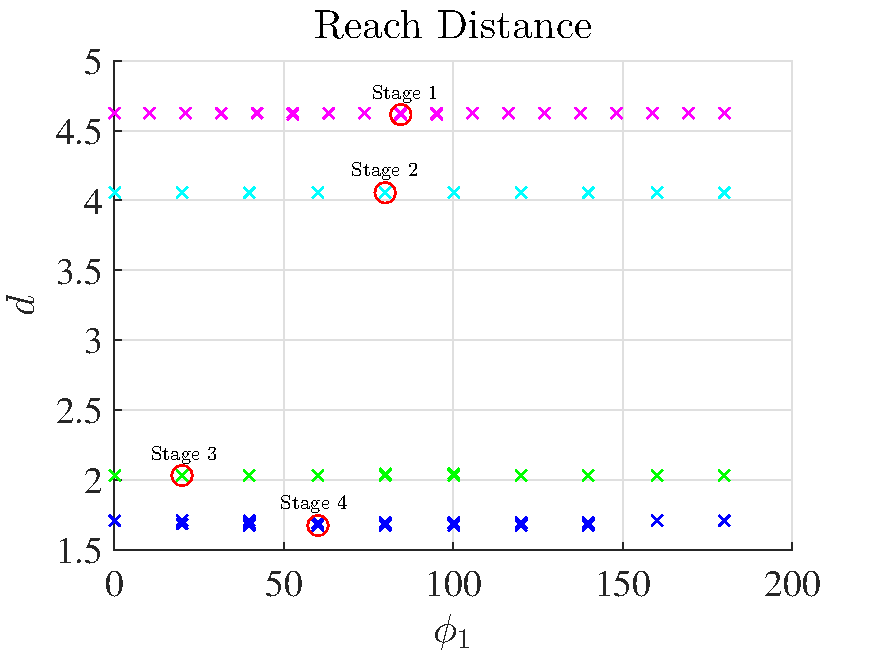
\includegraphics[width=\textwidth]{figures/2016_AAS/phi1.pdf} 
        \caption{ \( \phi_1 \)} \label{fig:phi1} 
    \end{subfigure}~
    \begin{subfigure}[htbp]{0.3\textwidth} 
        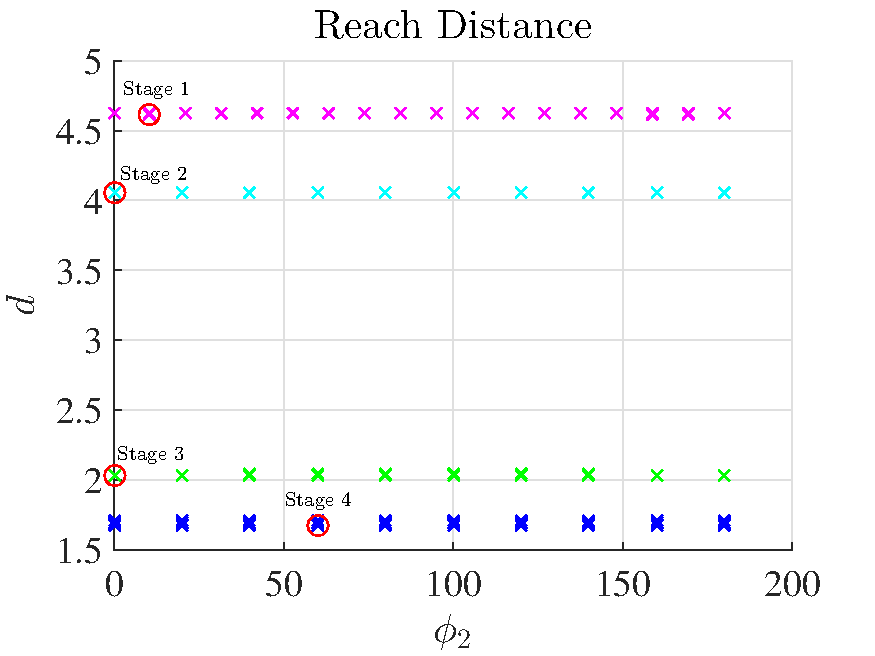
\includegraphics[width=\textwidth]{figures/2016_AAS/phi2.pdf} 
        \caption{\( \phi_2 \)} \label{fig:phi2} 
    \end{subfigure}~
    \begin{subfigure}[htbp]{0.3\textwidth} 
        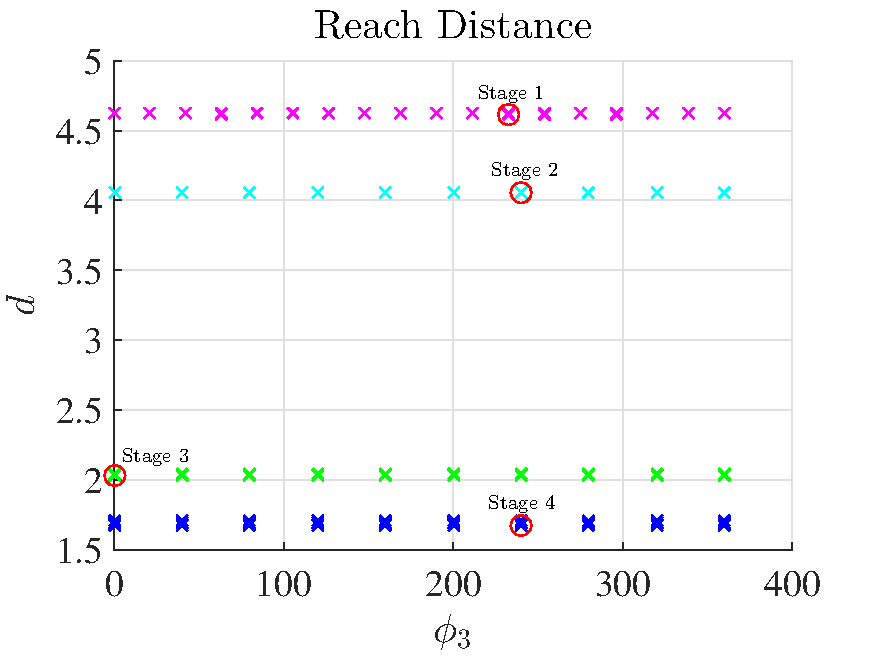
\includegraphics[width=\textwidth]{figures/2016_AAS/phi3.pdf} 
        \caption{\( \phi_3 \)} \label{fig:phi3} 
    \end{subfigure} 
    \caption{Variation of \(d(\vecbf{x}_f,\vecbf{x}_t)\) due to \( \phi_i\)}
    \label{fig:phi_distance} 
\end{figure}

The trajectory which minimizes \( d \) is indicated by the red circular markers in~\cref{fig:poincare_section,fig:phi_distance}.
Since the first reachability set does not include the target we use the minimum state from the first stage to initialize another reachability computation.
Once again we compute the reachability set by discretization of the angles \( \phi_i \) on the \Poincare section.
This second stage, represented by the cyan markers in~\cref{fig:poincare_section,fig:phi_distance}, further increases the \( x, z\) components but does not reach the target orbit.
As a result, a third and forth stage are generated in a similar manner and shown by the green and blue markers in~\cref{fig:poincare_section,fig:phi_distance}, respectively.
We can see in~\cref{fig:poincare_section} that the reachability set of the forth stage includes both the \( x \) and \( z\) components of the target periodic orbit.
At the same time there is a relatively large difference between the \( \dot{x} \), \( \dot{z} \), and \( z \) components of the forth stage and the target orbit.
In practice, this is not a large concern as we have direct control over the spacecraft velocity via the control input and the equatorial plane still remains within the reachability set of the transfer.

With the reachability set encompassing the target orbit, we can generate a final transfer to the target.
We use the minimum state calculated from the final stage to serve as the initial condition of the transfer.
A final optimal transfer is computed to satisfy the fixed terminal state \( \vc{x}(t_f) = \vc{x}_t \) and the bounded control magnitude constraint.
\Cref{fig:trajectory} shows the entire transfer trajectory, from the four reachable set trajectories as well as the final transfer to the target.
\begin{figure}[htbp] 
    \centering 
    \begin{subfigure}[htbp]{0.45\textwidth} 
        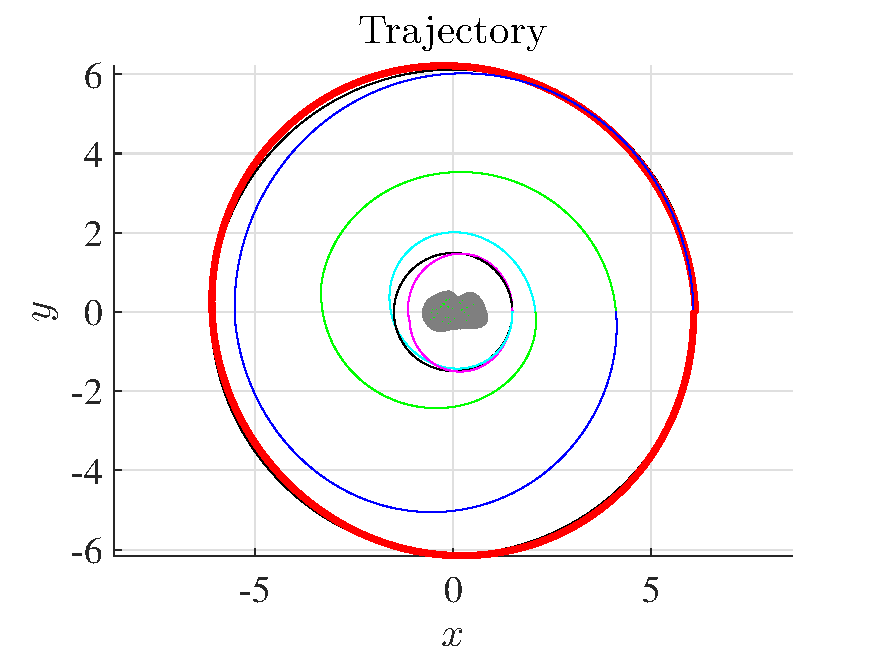
\includegraphics[width=\textwidth]{figures/2016_AAS/trajectory.pdf} 
        \caption{Equatorial view of transfer} \label{fig:trajectory_up} 
    \end{subfigure}~
    \begin{subfigure}[htbp]{0.45\textwidth} 
        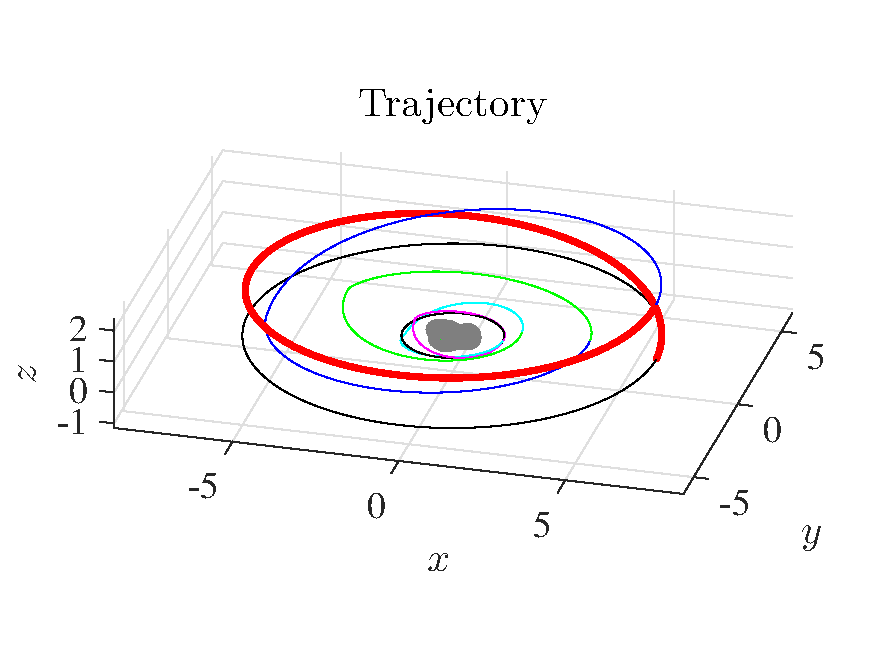
\includegraphics[width=\textwidth]{figures/2016_AAS/trajectory_3d.pdf} 
        \caption{Out of plane view} \label{fig:trajectory_3d} 
    \end{subfigure}~ 
    \caption{Complete transfer trajectory}
    \label{fig:trajectory} 
\end{figure}
It is interesting to note that while both the initial and target periodic orbit lie in the equatorial plane, the reachability trajectories show a relatively large out of plane component during the transfers.
In spite of this out of plane movement, the reachability set approaches and meets the target orbit. 
\begin{figure}
    \centering
    \includegraphics[width=0.45\textwidth]{figures/2016_AAS/control.pdf}
    \caption{Control history \label{fig:control}}
\end{figure}
\Cref{fig:control} shows the control input required during the maneuver.
We can see that the control constraint in~\cref{eq:control_constraint} is satisfied over the entire trajectory.


% TODO SE(3) Geometric control for landing/pointing
% Talk about attitude representations
% Talk about control on non-linear manifolds use IJCAS paper
% !TEX root = ../dissertation.tex

\chapter{Nonlinear Geometric Control}\label{sec:se3_control}

While there has been significant study of interplanetary transfer trajectories, relatively less analysis has been conducted on operations in the vicinity of asteroids.
The dynamic environment around asteroids is strongly perturbed and challenging for analysis and mission operations~\cite{scheeres1994,scheeres2000}.
Due to their low mass, which results in a low gravitational attraction, asteroids may have irregular shapes and potentially chaotic spin states.
As a result, typical approaches of assuming a inverse square gravitational model are at best inaccurate and at worst do not capture the true dynamic environment.
In addition, the vast majority of asteroid are difficult to track or measure using current ground-based optical sensors. 
Due to their small size, frequently less than \SI{1}{\kilo\meter}, and low albedo the reflected energy of these asteroids is insufficient for reliable detection or tracking.
Therefore, the dynamic model of the asteroid is relatively coarse prior to arrival of a dedicated spacecraft in the vicinity. 
As a result, any spacecraft mission to an asteroid is dependent on a robust dynamic simulation and must incorporate the ability to deal with uncertain forces and environments.

% talk about the coupling between attitude and translational states
Furthermore, since the magnitude of the gravitational attraction is relatively small, non-gravitational effects, such as solar radiation pressure or third-body effects, become much more significant.
As a result, the orbital environment is generally quite complex and it is difficult to generate analytical insights.
One key consideration is the coupling between rotational and translational states around the asteroid.
The coupling is induced due to the different gravitational forces experienced on various parts of the spacecraft.
The effect of the gravitational coupling is related to the parameter \(\epsilon = \frac{r}{R_c}\), where \(r\) is the characteristic spacecraft length and \(R_c\) is the orbital radius~\cite{hughes2004}.
For Earth based missions, the orbital radius is several orders of magnitude larger than the spacecraft length and \(\epsilon\) is small.
As a result, the corresponding gravitational moment is weak and can be neglected. 
Therefore, the translational and rotational equations of motion become decoupled and can be considered separately, significantly simplifying the analysis. 
However, for operations around an asteroid the orbital radius is much smaller, which leads to much larger values of \(\epsilon\) and much larger influence of the rotational and translational coupling.
References~\cite{elmasri2005} and~\cite{sanyal2004} investigated the coupling of an elastic dumbbell spacecraft in orbit about a central body, but only considered the case of a spherically symmetric central body.
Furthermore, the spacecraft model is assumed to remain in a planar orbit.
As result, these developments are not directly applicable to motion about an asteroid, which experience highly non-keplerian dynamics.

% now talk about the specific challenges of asteroid landing. there are lots of trajectory design papers and several have considered landing trajectories
An additional layer of complexity is the design of landing trajectories on asteroids.
Beginning with the first landing of NEAR Shoemaker on asteroid 433 Eros, there has been a concerted effort to develop techniques and methodologies for asteroid landing~\cite{dunham2002, kubota2006}.
There is already considerable knowledge on the planetary landing problem~\cite{acikmese2007, meditch1964, ingoldby1978}.
While conceptually similar, the landing of spacecraft on small bodies requires additional consideration. 
The surface of an asteroid is highly irregular and, as discussed previously, there is a large coupling between the translational and rotational dynamics of the vehicle, which is further exaggerated when close to the surface.
References~\cite{guelman1994, furfaro2013, zexu2012} consider the soft landing problem on an asteroid.
These approaches were primarily based on nonlinear control techniques which allowed for the development of closed loop controllers which enable landing.
However, only the translational dynamics of the body was considered and no notion of the attitude dynamics or it's coupling to the position is considered.
Furthermore, relatively simple gravitational models are used which make the results unsuitable for operations near irregular bodies.
In this chapter, we derive and develop a nonlinear geometric controller for the coupled dynamics of a spacecraft around an asteroid.

An additional layer of complexity is the design of landing trajectories on asteroids.
Beginning with the first landing of NEAR Shoemaker on asteroid 433 Eros, there has been a concerted effort to develop techniques and methodologies for asteroid landing~\cite{dunham2002, kubota2006}.
There is already considerable knowledge on the planetary landing problem~\cite{acikmese2007, meditch1964, ingoldby1978}.
While conceptually similar, the landing of spacecraft on small bodies requires additional consideration. 
The surface of an asteroid is highly irregular and, as discussed previously, there is a large coupling between the translational and rotational dynamics of the vehicle, which is further exaggerated when close to the surface.
References~\cite{guelman1994, furfaro2013, zexu2012} consider the soft landing problem on an asteroid.
These approaches were primarily based on nonlinear control techniques which allowed for the development of closed loop controllers which enable landing.
However, only the translational dynamics of the body was considered and no notion of the attitude dynamics or it's coupling to the position is considered.
Furthermore, relatively simple gravitational models are used which make the results unsuitable for operations near irregular bodies.
\section{Nonlinear Geometric Control}

A wide variety of control schemes have been proposed for asteroid landing missions~\cite{furfaro2013,li2011a}.
In addition, there are a  variety of controllers developed for systems evolving on \( \SE \)~\cite{lee2010,lee2013}.
In this paper, we extend their use from quadrotor aerial vehicles into the space domain. 
This approach addresses many of the issues associated with the related work on asteroid landings.
The geometric control methods used to develop these nonlinear controllers allow for the development of control systems for dynamic systems which evolve on nonlinear manifolds. 
By developing the control system directly on the nonlinear manifold, geometric control techniques provide unique advantages as compared to those developed using local coordinate representations.
Furthermore, the geometric controller avoids the chattering issues inherent in the previous sliding mode control approaches to asteroid landing.
In addition, rather than offering only a bounded stability guarantee, the proposed nonlinear geometric controller guarantees almost global tracking of the attitude and translational states. 
This stability guarantee is critical for mission operations passing close to the surface over highly irregular terrain.
Furthermore, the coupled geometric controller explicitly considers the attitude coupling of the body in contrast to many of the previous approaches.
We briefly summarize the key developments of the \( \SE \) control scheme and leave the detailed derivations to the source manuscripts~\cite{lee2010,lee2013}.
% TODO Basics of geometric control

% TODO Derive attitude and translation control seperately

% TODO Specifics for use in the asteroid case

\subsection{Spacecraft Dynamic Model}\label{sec:controlled_dynamic_model}
We consider the controlled motion of a rigid dumbbell spacecraft about a small body.
% TODO Add some citations for dumbbell for use in spacecraft
The dumbbell spacecraft consists of two masses connected by a massless rod and is a well-known representation of a multi body spacecraft.
Furthermore, the dumbbell model captures the important interactions of the coupling between orbital and attitude dynamics. 
As a result, this simple model is useful to capture the main characteristics of a wide variety of spacecraft configurations.
Typically, spacecraft have mass concentrated in a central structure, referred to as the bus, which houses the command and control system, actuators, fuel, sensors etc. 
In addition, comparatively light-weight solar panels extend from the bus to provide electrical energy from solar radiation. 
As a result, the distributed mass of the spacecraft is captured with the dumbbell representation.
In this section, we briefly review the polyhedron potential model and then present the derivation of the coupled dynamics of a dumbbell spacecraft about an asteroid.
In this work, we assume that the asteroid is much more massive than the spacecraft and its motion is not affected by that of the spacecraft.
This assumption allows us to treat the motion of the vehicle independently from that of the asteroid, instead of treating the more complicated full-body problem. 
% TODO Add link to dynamic model given in previous section
% The spacecraft model is the same as that defined in 

In this section, we develop a coupled control system to track a desired trajectory.
We assume that the desired trajectory, \( R_d(t), \vb{x}_d(t) \), are defined as the rotation matrix of the spacecraft body frame with respect to the inertial frame and the relative position of the spacecraft center of mass with respect to the asteorid and defined in the inertial frame, respectively.
In contrast to controller derived for quadrotor \gls{uav}, the attitude and translational motion is only lightly coupled in the spacecraft scenario.
From the dynamic equations of motion, the coupling between the translational and rotational dynamics is due to the gravitational moment on the spacecraft.
Furthermore, we assume that we have a fully actuated spacecraft such that we can apply a torque about all three rotational axes and a force in all three directions.
This is in contrast to \glspl{uav} where the system is underactuated and in order to produce certain translational forces the system must first rotate.
This is a relatively standard assumption in the astrodynamics community as most spacecraft contain seperate systems for attitude control, e.g.\ \glspl{rwa}, \glspl{cmg}, or cold gas thrusters, and translational control, e.g.\ cold-gas thrusters, electric propulsion, or large chemical rockets~\cite{hughes2004,wertz1978}.
However, there are also many examples of underactuated spacecraft, such as those with damaged components~\cite{petersen2015a} or cubesats with limited cost and/or size budgets.
% TODO Add citaitons for these papers
In these situations, there are a variety of methods to handle the underactuation, ranging from optimal control techniques, exploiting external forces, or utilizing multiple control loops.

The control system is presented as two seperate controllers, one for the attitude tracking and one for translational tracking. 
These controllers are computed independently and used to manuever the spacecraft for both asteroid reconstruction and landing.

\subsection{Attitude Control}
One distinctive feature of the attitude dynamics of rigid bodies is that it evolves on a nonlinear manifold.
The three-dimensional special orthogonal group, or \( \SO \), is the set of \( 3 \times 3 \) orthogonal matrices whose determinant is one.
This configuration space is non-Euclidean and yields unique stability properties which are not observable on a linear space.
For example, it is impossible to achieve global attitude stabilization using continuous time-invariant feedback~\cite{bhat2000}.

Attitude control is typically studied using a variety of attitude parameterizations, such as Euler angles or quaternions~\cite{shuster1993}.
Attitude parameterizations fail to represent the nonlinear configuration space both globally and uniquely~\cite{chaturvedi2011a}.
For example, minimal attitude representations, such as Euler angle sequences or modified Rodriguez parameters, suffer from singularities.
These attitude representations are not suitable for large angular slews.
In order to avoid singularities, the designer must carefully switch the chosen Euler angle sequence based on the operating region.
Another option is to artificially limit the operating region of the rigid body.
This ensures the system operates in a region free from singularities but limits the performance capabilities and ability to perform arbitrarily large angular maneuvers.
Quaternions do not have singularities but they double cover the special orthogonal group.
As a result, any physical attitude is represented by a pair of antipodal quaternions on the three-sphere.
An immediate implication of this ambiguity is that closed-loop stability properties derived using quaternions may not hold for the physical rigid body evolving on the true configuration space, namely the special orthogonal group.
During implementation, the designer must carefully resolve this non-unique representation in quaternion based attitude control systems to avoid undesirable unwinding behavior~\cite{bhat2000}.
This behavior is characterized by situations where the rigid body starts close to the desired attitude, yet the system unnecessarily rotates through a large angle in spite of a small initial error. 

The first step in designing a control system on a nonlinear manifold \( \Q \) is the selection of a proper configuration error function. 
This configuration error function, \( \Psi : \Q \times \Q \to \R \), is a smooth and proper positive definite function that measures the error between the current configuration and a desired configuration. 
Once an appropriate configuration error function is chosen, one can then define a configuration error vector and a velocity error vector in the tangent space \( \mathsf{T}_q \Q \) through the derivatives of \( \Psi \)~\cite{bullo2004}. 
With the configuration error function and vectors, the remaining procedure is analogous to nonlinear control design on Euclidean vector spaces. 
One chooses control inputs as functions of the state through a Lyapunov analysis on \Q.
The configuration error function used in this analysis has been used in~\cite{bullo2004,chaturvedi2009,lee2011a,kulumani2017a}.
In this section we summarize the properties developed previously and present several extensions for our use in the case of motion around an asteroid.

% trackign control
In order to determine the attitude control input, we first define a desired attitude tracking command.
An arbitrary smooth attitude tracking command \( R_d (t) \in \SO \in \R^3 \) are given as a function of time.
% TODO Add link to this equation in dynamic derivation
The corresponding angular velocity command is obtained using the attitude kinematics equation, \( \hat{\Omega}_d = R_d^T \dot{R}_d \).
With the desired attitude command, \( R_d(t), \Omega_d(t) \), we then define the errors associated with the attitude and angular velocity.
The attitude and angular velocity tracking errors must be careful chosen to remain on the tangent bundle of \SO.
\begin{prop}{Attitude Configuration Error Function}\label{prop:attitude_control_configuration_error}
First, an attitude error function \(A : \SO \times \SO  \to \R \), an attitude error vector \( e_R : \SO \times \SO \to \R \), and an angular velocity error \( e_\Omega : \SO \times \R^3 \times \SO \times \R^3 \) are defined as
\begin{subequations}\label{eq:attitude_error_function}
\begin{align}
    A(R, R_d) &= \frac{1}{2} G \tr{I - R_d^T R}, \label{eq:A} \\
    e_R &= \frac{1}{2} G \parenth{R_d^T R - R^T R_d^\vee}, \label{eq:eRA}\\
    e_\Omega &= \Omega - R^T R_d \Omega_d \label{eq:eWA}.
\end{align}
\end{subequations}
Then the following properties hold:
\begin{enumerate}
    \item \label{item:prop_A_psd} \( A \) is locally positive definite about \( R = R_d \) on \( \SO \).
    \item \label{item:prop_eRA} The variation of \( A \) with respect to a variation of \( \delta R = R \hat{\eta} \) for \( \eta \in \R^3 \) is given by
	\begin{align}\label{eq:dirDiff_A}
		\dirDiff{A}{R} &= \eta \cdot e_{R} ,
	\end{align}
	where the notation \( \dirDiff{A}{R} \) represents the directional derivative of $A$ with respect to $R$ along the direction $\delta R$.
    \item \label{item:prop_critical_points} The critical points of \( A \), where \( e_R = 0 \) are \( \braces{R_d} \cup \braces{R_d \exp(\pi \hat s) } \) for \( s \in \braces{e_1, e_2, e_3}\)
    \item \label{item:prop_A_quadratic} \( \Psi \) is a locally quadratic function, which means there exist constants \( 0 < n_1 \leq n_2 \) such that
    \begin{align}\label{eq:A_bound}
        n_1 \norm{e_R}^2 \leq \Psi(R) \leq n_2 \norm{e_R}^2 ,
    \end{align}
    for $0<\psi < h_1 $ where the constants \( n_1 = \frac{h_1}{h_2 + h_3} \) and \( n_2 = \frac{h_1 h_4}{h_5 \parenth{h1 - \psi} }\) for
	\begin{align*}
		h_1 &= \min\braces{g_1 + g_2, g_2 + g_3 , g_3 + g_1} ,\\
		h_2 &= \max\braces{\parenth{g_1 -g_2}^2,\parenth{g_2 -g_3}^2 , \parenth{g_3 -g_1}^2} ,\\
		h_3 &= \max\braces{\parenth{g_1 + g_2}^2, \parenth{g_2 + g_3}^2 , \parenth{g_3 + g_1}^2}, \\		
        h_4 &= \max\braces{g_1 + g_, g_2 +g_3, g+3 + g_1}, \\
        h_5 &= \max\braces{\parenth{g_1 + g_2}^2, \parenth{g_2 + g_3}^2, \parenth{g_3 + g_1}^2}.
	\end{align*}
\end{enumerate}
\end{prop}
\begin{proof}
    See~\Cref{proof:attitude_config_error}
\end{proof}

With the appropriate attitude configuration error we now present the error dynamics in~\cref{prop:attractive_error_dynamics}, which are used in the subsequent development of the nonlinear control system.
\begin{prop}\label{prop:attractive_error_dynamics}
    The attitude error dynamics for \( A(R, R_d), e_\Omega \) satisfy
	\begin{gather}
    	\diff{}{t} \parenth{A(R)} = e_{R_A} \cdot e_\Omega , \label{eq:A_dot} \\
		\diff{}{t} \parenth{e_{R_A}} = E(R, R_d) e_\Omega , \label{eq:eRA_dot} \\
        \diff{}{t} \parenth{e_\Omega} = J^{-1} \parenth{-\Omega \times J \Omega + u + W(R, \Omega) \Delta + M_{ext}} , \label{eq:eW_dot}
	\end{gather}
	where the matrix \(E(R,R_d)\in \R^{3\times3} \) is given by
	\begin{align}
		E(R,R_d) = &\frac{1}{2} \parenth{\tr{R^T R_d G}I - R^T R_d G} , \label{eq:E} \\
	\end{align}
\end{prop}
\begin{proof}
    See~\Cref{proof:attractive_error_dynamics}
\end{proof}

\subsubsection{Attitude Control without Disturbance}
With the appropriate attitude configuration error we now present an attitude controller for attitude stabailization and tracking. 
This controller assumes that there is no disturbances on the attitude dynamics, i.e.\ \( \Delta = 0 \).
\begin{prop}[Attitude Control]\label{prop:att_control}
	Given a desired attitude command \( \parenth{R_d, \Omega_d = 0} \) and positive constants \( k_R, k_\Omega \in \R \) we define a control input \( u \in \R^3 \) as follows
	\begin{gather}
        u = -k_R e_R - k_\Omega e_\Omega + \Omega \times J \Omega - M_{ext}. \label{eqn:nodist_control}
	\end{gather}
	Then the zero equilibrium of the attitude error is asymptotically stable, and the inequality constraint is always satisfied.
\end{prop}
\begin{proof}
See~\Cref{proof:att_control}
\end{proof}

\subsection{Constrained Attitude Control}

Many physical rigid body systems must perform large angular slews in the presence of state constraints.
For example, autonomous spacecraft or aerial systems are typically equipped with sensitive optical payloads, such as infrared or interferometric sensors.
These systems require retargeting while avoiding direct exposure to sunlight or other bright objects.
In addition, many ground based attitude testing environments, such as air bearing platforms, must operate in the presence of physical obstructions.
Determining a satisfactory attitude control maneuver in the presence of state constraints is a challenging task.
The removal of constrained regions from the rotational configuration space results in a \textit{nonconvex} region.
The attitude control problem in the feasible configuration space has been extensively studied~\cite{bullo2004,MayTeePaCC11,LEEITAC15}.
However, the attitude control problem in the presence of constraints has received much less attention.

% discuss how previous papers (mcinnes and lee/meshabi) have short comings
Several approaches have been developed to treat the attitude control problem in the presence of constraints.
A conceptually straightforward approach is used in~\cite{hablani1999} to determine feasible attitude trajectories prior to implementation.
The algorithm determines an intermediate point such that an unconstrained maneuver can be calculated for each subsegment.
Typically, an optimal or easily implementable on-board control scheme for attitude maneuvers is applied to maneuver the vehicle along these segments.
In this manner, it is possible to solve the constrained attitude control problem by linking several intermediary unconstrained maneuvers.
While this method is conceptually simple, it is difficult to generalize for an arbitrary number of constraints.
In addition, this approach is only applicable to problems where the selection of intermediate points are computationally feasible.

The approach in~\cite{frazzoli2001} involves the use of randomized motion planning algorithms to solve the constrained attitude control problem.
A graph is generated consisting of vertices from an initial attitude to a desired attitude. 
A random iterative search is conducted to determine a path through a directed graph such that a given cost, which parameterizes the path cost, is minimized.
The random search approach can only stochastically guarantee attitude convergence as it can be shown that as the number of vertices in the graph grow, the probability of nonconvergence goes to zero.
However, the computational demand grows as the size of the graph is increased and a new graph is required when constraints are modified. 
As a result, random search approaches are ill-suited to on-board implementation or in scenarios that require agile maneuvers.

Model predictive control for spacecraft attitude dynamics is another popular approach and has been studied in~\cite{guiggiani2014,kalabic2014,gupta2015}.
These methods rely on linear or non-linear state dynamics to repeatedly solve a finite-time optimal control problem.
Also known as receding horizon control, the optimal control formulation allows for a straight forward method to incorporate state and control constraints.
Computing the optimal control strategy over a moving horizon allows for a form of feedback type control rather than the more typical open-loop optimal control solution.
Due to the iterative nature of solving optimization problems, model predictive control methods are computational expensive and frequently apply direct optimization methods to solve the necessary conditions for optimality.
Therefore, these methods are complicated to implement and may not be suitable for real-time control applications.
  
% Previous potential function approach - developed using attitude parameterizations - singularities/ambiguities
Artificial potential functions are commonly used to handle kinematic constraints for a wide range of problems in robotics~\cite{rimon1992}.
The goal is the design of attractive and repulsive terms which drive the system toward or away from a certain obstacle, respectively.
The attractive function is designed to drive the system towards the desired state.
Similarly, a repulsive function is constructed such that the system is directed away from the constraints. 
The superposition of these functions allows one to apply standard feedback control schemes for stabilization and tracking.
More specifically, artificial potential functions have previously been applied to the spacecraft attitude control problem in~\cite{lee2011b,mcinnes1994}.
However, both of these approaches were developed using attitude parameterizations, namely Euler angles and quaternions, and as such, they are limited by the singularities of minimal representations or the ambiguity of quaternions.

This section is focused on developing an adaptive attitude control scheme in the presence of attitude inequality constraints on \(\SO\).
We apply a potential function based approach developed directly on the nonlinear manifold \(\SO\). 
By characterizing the attitude both globally and uniquely on \(\SO\), our approach avoids the issues of attitude parameterizations, such as kinematic singularities and ambiguities, and is geometrically exact. 
A configuration error function on \(\SO\) with a logarithmic barrier function is proposed to avoid constrained regions. 
Instead of calculating a priori trajectories, as in the randomized approaches, our approach results in a closed-loop attitude control system. 
This makes it ideal for on-board implementation on UAV or spacecraft systems. 
In addition, unlike previous approaches our control system can handle an arbitrary number of constrained regions without modification.
This approach results in a conceptually simple obstacle avoidance scheme which extends the previous work of artificial potential functions on Euclidean spaces to the special orthogonal group.
Furthermore, we use this new configuration error function to design an adaptive update law to enable attitude convergence in the presence of uncertain disturbances. 

\paragraph{State Inequality Constraint}\label{sec:state_inequality_constraint}
The two-sphere is the manifold of unit-vectors in \( \R^3 \), i.e., \( \Sph^2 = \{ q \in \R^3 \,  \vert \, \norm{q} = 1 \}\).
We define \( r \in \Sph^2 \) to be a unit vector from the mass center of the rigid body along a certain direction and it is represented with respect to the body-fixed frame.
For example, \( r \) may represent the pointing direction of an on-board optical sensor.
We define \( v \in \Sph^2 \) to be a unit vector from the mass center of the rigid body toward an undesired pointing direction and represented in the inertial reference frame.
For example, \( v \) may represent the inertial direction of a bright celestial object or the incoming direction of particles or other debris.
It is further assumed that optical sensor has a strict non-exposure constraint with respect to the celestial object.
We formulate this hard constraint as
\begin{align}
	r^T R^T v \leq \cos \theta , \label{eqn:constraint}
\end{align}
where we assume \( \ang{0} \leq \theta \leq \ang{90}  \) is the required minimum angular separation between \( r \) and \( R^T v \). 
The objective is to a determine a control input \( u \) that stabilizes the system from an initial attitude \( R_0 \) to a desired attitude \( R_d \) while ensuring that~\cref{eqn:constraint} is always satisfied.

\paragraph{Constrained Attitude Error Function}
To handle the attitude inequality constraint, we propose a new attitude configuration error function. 
More explicitly, we extend the trace form used in~\cite{bullo2004,LeeITCST13} and presented in~\Cref{prop:attitude_control_configuration_error} for attitude control on \(\SO\) with the addition of a logarithmic barrier function. 
Based on the proposed configuration error function, a nonlinear geometric attitude controller is constructed. 
A smooth control system is first developed assuming that there is  no disturbance, and then it is extended to include an adaptive update law for stabilization in the presence of unknown disturbances. 
The proposed attitude configuration error function and several properties are summarized as follows.
\begin{prop}[Constrained Attitude Error Function] \label{prop:repulsive_configuration_error}
Define an attitude error function \( \Psi : \SO \to \R \), an attitude error vector \( e_R \in \R^3 \), and an angular velocity error vector \( e_\Omega \in \R^3 \) as follows:
\begin{gather}
	\Psi(R, R_d) = A(R, R_d) B(R) , \label{eq:psi} \\
	e_R = e_{R_A} B(R) + A(R,R_d) e_{R_B} , \label{eq:eR} \\
	e_\Omega = \Omega , \label{eq:eW}
\end{gather}
with
\begin{gather}
	B(R) = 1 - \frac{1}{\alpha} \ln \left( \frac{\cos \theta -  r^T R^T v}{1 + \cos \theta}\right). \label{eq:B} \\
	e_{R_B} = \frac{\left( R^T v\right)^\wedge r}{\alpha \left(r^T R^T v - \cos \theta \right)}. \label{eq:eRB} 
\end{gather}	
where \( \alpha \in \R \) is defined as a positive constant.
Then, the following properties hold
\begin{enumerate}
	\item \label{item:prop_psi_psd} \(\Psi\) is positive definite about \( R = R_d\) on $\SO$.
	\item \label{item:prop_erb} The variation of \( B(R) \) with respect to a variation of \( \delta R = R \hat{\eta} \) for \( \eta \in \R^3 \) is given by
	\begin{align}\label{eq:dirDiff_B}
		\dirDiff{B}{R} &= \eta \cdot e_{R_{B}}.
	\end{align}
    \item \label{item:prop_psi_quadratic} \( \Psi \) is a locally quadratic function, which means there exist constants \( 0 < n_1 \leq n_2 \) such that
    \begin{align}\label{eq:psi_bound}
        n_1 \norm{e_R}^2 \leq \Psi(R) \leq n_2 \norm{e_R}^2 ,
    \end{align}
    on the neighborhood $D$ of the desired attitude \( R_d \)
    \begin{align}\label{eq:psi_quadratic_domain}
        D = \braces{R\in\SO  \vert \Psi < \psi < h_1, r^T R^T v < \beta < \cos \theta}
    \end{align}
    for $0<\psi < h_1 $ and $0< \beta<\cos\theta$. 
\end{enumerate}
\end{prop}
\begin{proof}
    See~\Cref{proof:repulsive_configuration_error}
\end{proof}

\Cref{eqn:psi} is composed of an attractive term, \( A (R) \) toward the desired attitude, and a repulsive term, \( B(R) \) away from the undesired direction \( R^T v \).
In order to visualize the attitude error function on \( \SO \), we utilize a spherical coordinate representation.
Recall, that the spherical coordinate system represents the position of a point relative to an origin in terms of a radial distance, azimuth, and elevation.
This coordinate system is commonly used to define locations on the Earth in terms of a latitude and longitude.
Similarly, the positions of celestial objects are defined on the celestial sphere in terms of right ascension and declination. 
\begin{figure}[htbp]%
    \centering 
    \subcaptionbox{Attractive \( A(R) \) \label{fig:attract_error} }{\includegraphics[trim={8mm 2mm 8mm 2mm}, clip, width=0.3\textwidth]{figures/2016_IJCAS/attract_error.pdf}}
    \subcaptionbox{Repulsive \( B(R) \) \label{fig:avoid_error} }{\includegraphics[trim={8mm 2mm 8mm 2mm}, clip, width=0.3\textwidth]{figures/2016_IJCAS/avoid_error.pdf}}
    \subcaptionbox{Combined \( \Psi \) \label{fig:combined_error} }{\includegraphics[trim={8mm 2mm 8mm 2mm}, clip, width=0.3\textwidth]{figures/2016_IJCAS/combined_error.pdf}}%
    \caption{Visualization of Configuration Error Functions using spherical coordinate representation}
    \label{fig:config_error} 
\end{figure}%
We apply this concept and parameterize the rotation matrix \( R \in \SO \) in terms of the spherical angles \( \SI{-180}{\degree} \leq \lambda \leq \SI{180}{\degree}  \) and \( \SI{-90}{\degree} \leq \beta \leq \SI{90}{\degree} \). 
Using the elementary Euler rotations, the rotation matrix is now defined as \( R = \exp( \lambda \hat{e}_2) \exp( \beta \hat{e}_3) \).
We iterate over the domains of \( \lambda\) and \(\beta\) in order to rotate the body-fixed vector \( r \) throughout the two-sphere \( \S^2 \).
Applying this method,~\cref{fig:config_error} allows us to visualize the error function on \( \SO \).
The horizontal axes of~\cref{fig:config_error} represent the domain of the spherical angles \( \lambda \) and \( \beta \) in degrees, while the vertical axes represent the unitless magnitude of the error functions defined in~\cref{eq:psi,eq:A,eq:B}.
The attractive error function, given by~\cref{eq:A}, has been previously used for attitude control on \(\SO\).
The potential well of \( A(R)\) is illustrated in~\cref{fig:attract_error}, where the desired attitude lies at the minimum of \( A(R) \).

To incorporate the state inequality constraints we apply a logarithmic barrier term.
Barrier functions are typically used in optimal control and motion planning applications.
A visualization of the repulsive error function is presented in~\cref{fig:avoid_error} which shows that as the boundary of the constraint is neared, or \( r^T R^T v \to \cos \theta \), the barrier term increases, \( B \to \infty\).
We use the scale factor~\(\frac{1}{1+\cos \theta} \) to ensure that \( \Psi \) remains positive definite.
The logarithmic function is popular as it quickly decays away from the constraint boundary.
The positive constant \( \alpha \) serves to shape the barrier function.
As \( \alpha \) is increased the impact of \( B(R) \) is reduced away from the constraint boundary. 
The superposition of the attractive and repulsive functions is shown in~\cref{fig:combined_error}.
The control system is defined such that the attitude trajectory follows the negative gradient of \( \Psi \) toward the minimum at \( R = R_d \), while avoiding the constrained region.

While~\cref{eqn:B} represents a single inequality constraint given as~\cref{eqn:constraint}, it is readily generalized to multiple constraints of an arbitrary orientation. 
For example, the configuration error function can be formulated as $\Psi=A[1+\sum_i C_i]$, where $C_i$ has the form of $C_i=B-1$ for the $i$-th constraint. 
In this manner, one may enforce multiple state inequality constraints, and we later demonstrate this through numerical simulation. 
This is in contrast to many previous approaches which are computationally difficult to extend to situations with multiple constraints.
We present the dynamics of the combined configuration error function in~\Cref{prop:error_dyn}, which are used in the subsequent development of the nonlinear control system.

\begin{prop}[Constrained Error Dynamics]\label{prop:repulsive_error_dynamics}
	The attitude error dynamics for \( \Psi, e_R, e_\Omega \) satisfy 
	\begin{gather}
		\diff{}{t} \parenth{\Psi} = e_R \cdot e_\Omega , \label{eq:psi_dot}\\
		\diff{}{t} \parenth{e_R} = \dot{e}_{R_A} B + e_{R_A} \dot{B} + \dot{A}e_{R_B} + A \dot{e}_{R_B} , \label{eq:eR_dot} \\
		\diff{}{t} \parenth{e_{R_B}} = F(R) e_\Omega , \label{eq:eRB_dot} \\
		\diff{}{t} \parenth{B(R)} = e_{R_B} \cdot e_\Omega , \label{eq:B_dot} \\
	\end{gather}
	where the matrix \(F(R) \in \R^{3\times3} \) is given by
	\begin{align}
		F(R) = &\frac{1}{\alpha \parenth{r^T R^T v - \cos \theta}} \left[\parenth{v^T R r} I - R^T v r^T + \frac{R^T \hat{v} R r v^T R \hat{r}}{\parenth{r^T R^T v - \cos \theta}}\right]. \label{eq:F}
	\end{align}
\end{prop}
\subsection{Attitude Pointing modes}

This positive definite function parameterizes the error between the current attitude, \( R \), and the desired attitude command \( R_d \).
Using the variations of \( \Psi \) gives the attitude tracking error vector \( e_R \in \R^3 \) as
\begin{align}\label{eq:attitude_error_vector}
    e_R = \frac{1}{2} \parenth{R_d^T R - R^T R_d^\vee}.
\end{align}
After further manipulation and using the attitude kinematics equation from~\cref{eq:attitude_kinematics}, it is possible to define the angular veloicty tracking error \( e_\Omega \in \R^3 \) as
\begin{align}\label{eq:angular_velocity_error_vector}
    e_\Omega = \Omega - R^T R_d \Omega_d.
\end{align}
With the properly defined attitude error vectors the rotational control input is defined as 
\begin{align*}\label{eq:rotational_control}
    \vb{u}_m = - k_R e_R - k_\Omega e_\Omega + \Omega \times J \Omega - J \parenth{\hat{\Omega} R^T R_d \Omega_d - R^T R_d \dot{\Omega}_d} - \vb{M}_1 - \vb{M_2} 
\end{align*}
where \( k_R, k_\Omega \) are positive controller constants.

\subsection{Translation Control}
The translational control input is defined in a similar manner. 
First we define a smooth tracking command \( x_d(t) \in \R^3 \), which defines the desired position of the spacecraft in the inertial frame.
The tracking error vectors are easier to define as they evolve on a Euclidean space rather than a nonlinear manifold and are given by
\begin{align}
    e_x = x - x_d ,\\
    e_v = v - \dot{x}_d.
\end{align}
With the error variables, the translational control input is then given by
\begin{align}\label{eq:translation_control}
    \vb{u}_f = - k_x e_x  - k_v e_v + ( m_1  + m_2 ) \ddot{x}_d - \vb{F}_1 - \vb{F}_2 ,
\end{align}
where \( k_x, k_v \) are positive constants. 
The control gains are chosen based on the desired closed-loop system response. 
A variety of techniques are available to choose these gains, but a simple linear analysis offers a straightforward and systematic approach to choosing suitable values. 
We use the control inputs defined in~\cref{eq:translation_control,eq:rotational_control} and substitute them into the dynamic equations of motion in~\cref{eq:translational_dynamics,eq:attitude_dynamics}.
This results in the dynamics of the error variables and the gains are chosen to ensure the error behavior meets desired performance criteria, such as percent overshoot or settling time~\cite{nise2004}.


\section{Numerical Example}

% TODO Disucss numerical implementation
Typically, spacecraft missions require extensive interaction from ground based human operators. 
This interaction ranges from system health checks to navigation and hardware commands.
In addition, there is frequently a large group of analysts in support of any given mission. 
A wide variety of factors make human in the loop control of spacecraft especially difficult.
First, the vast distances cause significant time delays which render it impossible to react immediately to events experienced by the spacecraft. 
Furthermore, deep space missions are designed for continuous mission operations for many years or even decades. 
It is becoming increasingly difficult to maintain trained and knowledgeable staff for several decades in order to support a single mission.
In addition, these operators become increasingly scarce as the contemporary hardware and software tools surpass those of these decades old spacecraft. 
As a result, there is a large focus on completely autonomous spacecraft systems.

We present a numerical simulation of a rigid dumbbell about asteroid Itokawa.
The dumbbell spacecraft is composed of two equal masses, \( m_1, m_2 = \SI{500}{\kilo\gram} \), seperated by \( l = \SI{3}{\meter} \).
The dumbbell body frame is defined with the first body fixed axis, \( \vb{b}_1 \), originating at the center of mass of the spacecraft and directed along the vector from \( m_1 \) towards \( m_2 \).
The other two axes of the spacecraft fixed frame are chosen orthogonal to the \( \vb{b}_1 \) and lie in the plane orthogonal to the dumbbell axis of symmetry. 
A camera, using the parameters from~\cref{tab:camera_parameters}, is aligned with the \( \vb{b}_1 \) axis and used to feed image data to the ORB-SLAM system.
A numerical simulation is used to demonstrate the geometric control of the coupled motion of the spacecraft, and the ability to estimate the motion of the spacecraft from monocular imagery.

The initial condition of the spacecraft is defined as
\begin{align}
    \vb{x}_0 &= \begin{bmatrix} 0 & -2.550 & 0 \end{bmatrix} \si{\kilo\meter}, \\
    R_0 &= \exp {\frac{\pi}{2} \vb{e}_3}.
\end{align}
The spacecraft begins on the inertial \( \vb{e}_2 \) axis and initially pointing at the asteroid. 
A tracking command is designed to transition the spacecraft towards the asteroid fixed \( \vb{f}_1  \) axis followed by a vertical descent along towards the asteroid surface.
The translational command is divided into two stages, a traverse step where the spacecraft follows a trajectory to align itself with the \( \vb{f}_1 \) axis and a landing step where the spacecraft follows a constant velocity descent towards the surface. 
The desired position command is defined as
\begin{align}
    \vb{x}_d = 
    \begin{cases}
        2.550 \begin{bmatrix} \sin{\omega t} & -\cos{\omega t} & 0 \end{bmatrix}, & t \leq t_d \\
        R_A \begin{bmatrix} \frac{2}{t_d} (t - t_d) + 2.550 & 0 & 0 \end{bmatrix}, & t > t_d , 
    \end{cases}
\end{align}
where \( \omega = \frac{\pi}{2 t_d} \), \( t_d \) is the time from the simulation start when the constant velocity descent should begin, and \( t \) is the simulation time step.

The desired attitude command is chosen such that the spacecraft camera axis, \( \vb{b}_1 \), is directed along the nadir towards the asteroid.
It is sufficient to define two orthogonal vectors to uniquely determine the attitude of the spacecraft.
The \( \vb{b}_{3d} \) vector is chosen to lie in the plane spanned by \(\vb{b}_{1d} \) and \( \vb{e}_3 = \vb{f}_3 \).
The desired attitude command is defined as
\begin{align}
    \vb{b}_{1d} &= - \frac{\vb{x}}{\norm{\vb{x}}} , \\
    \vb{b}_{3d} &= \frac{\vb{f}_3 - \parenth{\vb{f}_3 \cdot \vb{b}_{1d}} \vb{b}_{1d}}{\norm{\vb{f}_3 - \parenth{\vb{f}_3 \cdot \vb{b}_{1d}} \vb{b}_{1d}}}, \\
    \vb{b}_{2d} &= \vb{b}_{3d} \times \vb{b}_{1d} , \\
R_d &= \begin{bmatrix} \vb{b}_{1d} & \vb{b}_{2d} & \vb{b}_{3d} \end{bmatrix}.
\end{align}
The camera axis is aligned with the spacecraft \( \vb{b}_ 1 \) axis, which is direted towards the asteroid, throughout the landing trajectory as the spacecraft moves in the equatorial plane of the asteroid.

The simulation is carried out over \SI{7200}{\second} with the spacecraft following a circular trajectory for the first \SI{3600}{\sec} before vertically descending in the body fixed frame for the last \SI{3600}{\second}.
\Cref{fig:true_landing_trajectory} shows a view from the positive \( \vb{f}_3 \) pole of the asteroid of the simulated trajectory. 
The position of the center of mass of the dumbbell is shown in blue, while the pointing direction of the camera axis is defined in red. 
The attitude of the dumbbell is displayed at several points along the trajectory demonstraiting the pointing of the camera. 
Furthermore, asteroid Itokawa is shown in its final orientation at the completion of the landing simulation. 
\Cref{fig:pos_components} shows that the nonlinear controller is able to accurately track the desired translational trajectory for the duration of the simulation.
\begin{figure}[htbp]
    \captionsetup[subfigure]{position=b}
    \centering
    \subcaptionbox{Planar view of landing trajectory\label{fig:true_landing_trajectory}}{\includegraphics[width=0.5\textwidth]{figures/2017_AAS_fall/traj_fig.pdf}}
    \subcaptionbox{Position of spacecraft in the inertial frame\label{fig:pos_components}}{\includegraphics[width=0.5\textwidth]{figures/2017_AAS_fall/pos_fig.pdf}}
    \caption{Landing trajectory to asteroid Itokawa~\label{fig:position}}
\end{figure}

% TODO Shape reconstruction using LIDAR measurements
% !TEX root = ../dissertation.tex

\chapter{Asteroid Shape Reconstruction and Refinement}\label{sec:shape_reconstruction}
This chapter is devoted to introducing the application of computational geometry to asteroid shape reconstruction.
The polyhedron potential model is the standard approach for missions operating around small-bodies.
As a result, the determination of an accurate shape is critical for both the gravitational model as well as any low-altitude operations.
Prior to any spacecraft mission to an asteroid, extensive ground measurements will be collected on the potential target.
These measurements will be used to not only accurately track the small body in space, but also to generate an approximate shape model of the body. 
However, these shape models are relatively coarse and only provide a general shape of the body and lack detailed features critical for safe and accurate landing.
Typically, a significant portion of the mission life cycle is devoted solely to terrain mapping and shape modeling.
For example, the NEAR mission devoted the first five months in the vicinity of asteroid Eros to mapping and shape estimation~\cite{antreasian2002} while the Hyabusa mission spent three months near asteroid Itokawa~\cite{barnouin-jha2008} using a \gls{lidar} sensor to accurately measure the surface.
However, for certain types of missions, such as asteroid mitigation~\cite{garshnek2000,pitz2014} or multiple body surveying~\cite{stuart2011a,stuart2016} this type of extensive mapping is not feasible.
This chapter develops an efficient method for the reconstruction of an asteroid shape given \gls{lidar} measurements.
The approach enables a spacecraft to arrive at an asteroid with a very coarse shape model, autonomously measure the surface to rebuild the shape, and finally determine an appropriate landing location and descend to the surface.
We utilize many concepts and development from computational geometry for a variety of purposes, from simply representing and operating on data structures to efficient computational algorithms.

Computational geometry is defined as the systematic study of algorithms and data structures for geometric objects~\cite{berg2008}.
A specific focus is on exact algorithms that are asymptotically fast.
Computational geometry emerged from the fields of computer science in the late 1969s.
Since that time, the field has grown considerably and has found applications in a large variety of domains, suchs as computer graphics, \gls{gis}, robotics, \gls{CAD}, computer vision, and others.

The general approach to solving computational geometric problem is based on two key components.
The first is a deep understanding of the geometric properties of the problem and the second is the proper application of efficient algorithms and/or data structures.
In this chapter, we use several algorithms and approaches from computational geometry to simulate a spacecraft mounted \gls{lidar} sensor around an asteroid.
The first task is to simulate the measurement from the \gls{lidar} of the surface of the asteroid.
This will utilize the well known method of \gls{raycasting} to find the intersection of a mesurement ray with the surface.
Given the surface intersection, these measurements will be incrementally incoprorated into the asteroid shape model while maintaining the required topological constraints.

\section{Mathematical Background}

The \gls{polyhedron} potential model is the standard approach for missions around asteroids~\cite{werner1994,werner1996}.
As a result, an understanding of the properties of \glspl{polyhedron} and the methods to construct them are critical.
The construction and update of the asteroid shape model must produce a valid three-dimensional model.
For example, the geometric model must not contain any dangling edges or surfaces~\cite{mortenson1997}.
A consideration of the topology of the model is crucial, and features such as homogenity and connectivity are important properties to consider.
A \gls{polyhedron} is an arrangement of \glspl{polygon} such that two and only two \glspl{polygon} meet at an edge~\cite{mortenson1997}.
Furthermore, it is possible to travese the surface of the \gls{polyhedron} by crossing it's edges to eventually cross each face in a continuous path.

\subsection{Small Body Shape Modeling}\label{sec:shape_model}
% TODO Describe asteroid shape representation

Asteroids can have a wide variety of shapes, and most are vastly different than that of a sphere or ellipsoid.
\Cref{fig:irregular_asteroids} shows two examples of small solar system bodies that have highly irregular shapes.
As a result of these highly variable shapes, an adaptable format is required to represent the wide variety of surface shapes and surface features.
\begin{figure}[h]
    \centering
    \subcaptionbox{Asteroid Itokawa\label{fig:itokawa}}{\includegraphics[height=0.3\textheight,width=0.5\textwidth, keepaspectratio]{figures/mathematical_background/eso1405b.jpg}}~
    \subcaptionbox{Comet 67/Churyumov-Gerasimenko\label{fig:67p}}{\includegraphics[height=0.3\textheight,width=0.5\textwidth,keepaspectratio]{figures/mathematical_background/comet67pcgin.jpg}}
    \caption{Examples of the non-ellipsoidal shapes of small solar system bodies. Both asteroids and comets will tend to have vastly irregular shapes due to their low mass and violent histories of impacts and collisions~\label{fig:irregular_asteroids}}
\end{figure}
The scientific community describes asteroid shape using the facet-vertex model.
This approach is an efficient representation of the more general notion of a polyhedron from geometry.
In this section, we define the notion of the polyhedron and some specifics of the format used in the astrodynamics community.

A polyhedron is a generalization of a two-dimensional polygon to three-dimensions~\cite{orourke1998}.
It is the region of space with a boundary defined by a surface of a finite number of polygonal faces.
The surface of the polyhedron is composed of three types of primitive objects: zero-dimensional points called vertices, one-dimensional segments called edges, and two-dimensional polygons called faces or facets.
Furthemore, without any loss of generality we assume each face is a convex polygon since any nonconvex face can be divided into smaller convex faces.
A valid polyhedron, in the context of asteroid shape models, must satisfy several constraints.
These constraints define the relationship between each of the types of primitives which make up the polyhedron surface.
The primitives must intersect ``properly'' and the local and global topology must be ``proper''.
For asteroid shape model we further assume that each face is a triangular polygon. 
Again, this does not limit generality as any polygon can be divided into a series of planar triangles.

The intersection of each face must be one of the following:
\begin{itemize}
    \item the faces are disjoint and do not intersect, or
    \item the faces meet at a single vertex, or
    \item the faces share two vertices and a common edge.
\end{itemize}
These intersection constraints automatically ensures that all edgeds and vertices intersect properly.
For example, edges that do not extend across an entire face or faces with penetrate would be improper and invalid.
Some examples of invalid polyhedron are shown in~\cref{fig:improper_polyhedrons}.
\begin{figure}[h]
    \centering
    \subcaptionbox{Point lies on two surfaces\label{fig:two_surfaces}}{\includegraphics[width=.33\textwidth]{figures/computational_geometry/hanging_face.png}}~
    \subcaptionbox{The neighborhood around this point is not homemorphic to a disk\label{fig:knotted_polyhedron}}{\includegraphics[width=.33\textwidth]{figures/computational_geometry/pinched.png}}~
    \subcaptionbox{The surface is not closed\label{fig:open_polyhedron}}{\includegraphics[width=.33\textwidth]{figures/computational_geometry/open.png}}
    \caption{Three example objects which are not polyhedra. For each example, the neighborhood about each point is not homeomorphic to an open disk.~\label{fig:improper_polyhedrons}}
\end{figure}

The second constraint is related to the local topology around each point on the surface of the polyhedron.
In order to be locally proper, the neighborhood about any point on the surface of the polyhedron should be homeomorphic to a two-dimensional disk.
A neighborhood about any point on the surface is defined as an arbitrarily small subset or region of the surface which surrounds the point.
Every point on the surface should have a neighborhood which is topologically equivalent to a two dimensional disk.
The notion of equivalency is mathematically captured using the property of homeomorphism.
A homemorphism between two regions is a continous stretching or bending, without tearing or cutting, from one shape to another.
For example, it is possible to turn a circle into a square by a continuous stretching and bending of the shape.
However, it is not possible to transform a sphere into a torus, as this would require a hole to be created in the surface of the sphere.
The neighborhood about any point on the surface of the polyhedron should be equivalent to that of a two-dimensional disk.
A surface where this true for all points is called a \textit{two-manifold}, of a which the surface of a polyhedron is a subset.

The final constraint is related to the global structure of the surface in contrast to the local neighborhood of a point.
The surface must be connected, closed, and bounded.
In this sense, a connected surface is one where it is possible to travel from one point to any other point of the surface without leaving the surface. 
As a result, this will rule out any shapes with non-connected faces, such as a cube with a hollow interior/surface.
For example, on the outer surface of the cube it is not possible to reach a point on the interior surface. 
Combined with an assumption that there are a finite number of faces automatically ensures a closed and bounded surface. 
Note that these conditions do not in general rule out the possibility of holes passing completely through the object.
For example, a torus, or a donute shape, is also considered a polyhedron.
The key difference between a hole and a cavity is that there are no disconnected surfaces and as a result a polyhedron can have any number of such holes. 
In practice, we tend to limit our analysis to polyhedron with no holes, or with a genus of zero.

% TODO Euler's constant description

\subsection{Polyhedron Data Structures}\label{sec:polyhedron_data_structures}
While the shape of the asteroid will be represented mathematically as a polyhedron, we are still left with the issue of representing this shape in digital form. 
The eventual computational efficiency and memory consumption of the subesequent sections is heavily dependent on the underlying data structure used to represent the surface.
In this section, we review some of the basic requirements and features of any data structure.
In addition, we summarize the ones most popular in the astrodynamics community and the halfedge data structure which we use in this work.

The requirements for any surface/mesh data structure vary between applications and are designed to satisfy both topological and algorithmic requirements.
Some examples of topological considerations are the use of triangular/polygonal facets or the ability to represent manifold/non-manifold meshes.
Examples of algorithmic requirements include a consideration of the types of algorithms/processes that will make use of the data, such as visualization or operations that will modify or additional data to the various faces, edges, and vertices of the mesh.
The choice, and eventual design, of an appropriate data structure is evaluated on its ability to efficiently enable specific operations, such as distance or modification operations.
A wide variety of data structures have been developed to represent general polyhedron surfaces and can be classified as either \textit{face-based} or \textit{edge-based}.

The simplest method to represent a surface mesh is composed to storing the individual vertices which define each face of the surface.
In the specific case of a triangular mesh, this entails storing the three vertex coordinates of each face of the mesh, also called the \textit{face-set}~\cite{botsch2010}.
By assuming that the vertex coordinates are stored as double precision, or \SI{64}{\bit} values, results in \( 3 \cdot 3 \cdot 64 = \SI{576}{\bit} = \SI{72}{\byte}\) per triangular face.
% TODO Add reference to euler's formula
Equivalently, from Euler's formula, there is approximately twice as many faces as vertices, and this \textit{face-set} structure will require on average \SI{144}{\byte} per vertex.
A simple optimization is possible by reducing the redundancy in the representation.
Each vertex will duplicated as many times as the degree of the vertex.
This redundancy can be eliminated by storing a list of vertices, and to define the vertices of each face as an index/reference into this vertex list.
This results in the so called \textit{indexed face set} or \textit{shared-vertex} data structure.
In the case of triangular meshes and using double precision values, each vertex will require \(\SI{192}{\bit} = \SI{24}{\byte}\).
Vertex indices of each face can be stored using single precision, \( \SI{32}{\bit} = \SI{4}{\byte}\), values which resuts in a storage requirement of \( \SI{96}{\bit} = \SI{12}{\byte}\) per triangle.
This type of representation will therefore require on average approximately \( \SI{60}{\byte} \) per vertex, which is half the requirement of the \textit{face-set} data structure.
\begin{figure}
    \centering
    \includegraphics[width=\textwidth]{example-image-golden}
    \caption{Face based data structure look in PMP Fig2.3 or 2.4~\label{fig:face_based_data_structure}}
\end{figure}
Examples of this type of data structure include the \gls{stl}, \gls{obj}, and \gls{off} file formats.

While conceptually simple the face based data structure has several critical drawbacks.
It is difficult to determine the connectivity of individual vertices or faces of the mesh, which makes it ill-suited for most algorithms.
The vast of majority of computational geometry algorithms will require as a minimum~\cite{botsch2010}:
\begin{itemize}
    \item Access to individual vertices, edges and faces, as well as random access to any element.
    \item Enumeration of the edges of a single face.
    \item Access to the adjacent faces of an edge which enables access to the neighboring faces.
    \item Given an edge one must determine the two vertices which define the endpoints.
    \item Given a vertex one must determine all neighboring faces.
\end{itemize}
As a result, any application making use a face based data structure will need to store additional connectivity information in a seperate data structure.

In contrast to face-based structures, edge-based data structures store the connectivity information in the edges or halfedges~\cite{botsch2010,orourke1998,berg2008}.
By splitting each unorientated edge into two orientated halfedges, the halfedge data structure, or also known as the doubly-connected edge list, provides an efficient data structure for mesh based operations.
Each halfedge is ordered in a clockwise fashion around each face, typically such that the face normal is orientated outwards from the mesh.
In addition, each halfedge will also store a reference to:
\begin{itemize}
    \item The vertex it points to, or its target,
    \item its adjacent face,
    \item the next halfedge of the face in a counterclock wise direction,
    \item the previous halfedge of the face
    \item the opposite or incident halfedge.
\end{itemize}
In addition, each face stores the reference to one of its halfedges, while each vertex stores an outgoing halfedge. 
The halfedge data structure will require more memory in contrast to face based approaches it offers several advantages which make it ideal for computational geometry operations.

\subsubsection{Halfedge Data Structure}\label{sec:halfedge_data_structure}
A halfedge data structure allows us to iterate through all elements, vertices, edge, halfedge, or face, in a simple manner.
In addition, the halfge edge data structure can store arbitrary polygon meshes.
Furthermore, additional data can be attached to the elements as each is store explicitly.
Finally, the halfedge data structure allows for simple manipulation and modification of the underlying mesh, enabling operations such as mesh subdivision or simplification.
There are a number of publicly avaiable implementations of the halfedge data structure~\cite{cgalproject2018,botsch2002}.
We utilize the \texttt{Surface\_mesh} data structure implemented within the Computational Geometry Algorithms Library~\cite{sieger2011}.
This provides a well defined and highly optimzed data structure for the representation of the polyhedron shape of the asteroid.
Furthermore, the ability to incorporate additional properties enables us to efficently compute the polyheron potential model.
\begin{figure}
    \centering
    \includegraphics[width=\textwidth]{example-image-golden}
    \caption{Halfedge data structure look in PMP Fig3.4~\label{fig:halfedge_data_structure}}
\end{figure}

\begin{figure}
    \centering
    \includegraphics[width=\textwidth]{example-image-golden}
    \caption{Iterating over 1 ring of a vertex}
\end{figure}
% TODO Describe the halfedge data structure and Surface_mesh in more detail

\subsubsection{Wavefront OBJ files}
The OBJ format is a geometry definition file format used for a variety of computer modeling applications, and is regularly used by the asteroid community~\cite{neese2004}.
The basic format of the file is an ASCII file where the first \( N_v\) lines begin with \texttt{v} and define the three components of a vertex in the body fixed reference frame.
The following \( N_f\) lines begin with \texttt{f} and define the three indices of the vertices that make up the face.
The numbering of the vertices is implicitly defined by the order listed in the file, i.e. the vertices are defined from \( 1 \) to \( N_v\).
There are two main assumptions used by the asteroid community.
First, each face is triangular and second, the vertices are numbered in a counterclockwise fashion about each face.
This allows the outward facing normal to each face to be uniquely defined without any additional data.

This polyhedron model, captured using the OBJ format, allows for a much larger class of potential object shapes. 
The accuracy of the shape model can be arbitrarily improved by incorporating additional vertices and faces, which increase the resolution of the model in regions of high complexity.
The polyhedron model can capture arbitrary depressions, ridges, or holes through the asteroid.
Small bodies typically lack sufficient mass to create regular, spherical shapes, and exhibit a large variety in resulting shapes such as the examples shown in~\cref{fig:asteroid_shape}.
\begin{figure}
    \centering
    \subcaptionbox{4769 Castalia\label{fig:castalia}}{\includegraphics[width=0.33\textwidth]{figures/mathematical_background/castalia_isometric.jpg}}~
    \subcaptionbox{Geographus\label{fig:geographus}}{\includegraphics[width=0.33\textwidth]{figures/mathematical_background/geographus_isometric.jpg}}~
    \subcaptionbox{Golevka\label{fig:golevka}}{\includegraphics[width=0.33\textwidth]{figures/mathematical_background/golevka_isometric.jpg}}
    \caption{Polyhedron Shape Models for several asteroids~\label{fig:asteroid_shape}}
\end{figure}
Polyhedron shape models are available for several asteroids~\cite{neese2004,gaskell2008b}.
The quality and resolution is dependent on the measurement available of the body.
\Cref{fig:itokawa_radar} shows a polyhedron model of asteroid 25143 Itokawa based on ground radar measurements~\cite{neese2004}.
This model is composed of \num{6098} vertices and \num{12192} faces and captures the general ellipsoidal shape of the asteroid.
However, ground based measurements are unable to provide the resolution required to capture the fine details or even the asymmetry of asteroid Itokawa.
In contrast,~\cref{fig:itokawa_insitu} shows the model derived from in-situ measurements from optical sensor of the Hyabusa spacecraft~\cite{gaskell2008a}.
It is composed of \num{1579014} vertices and \num{3145728} faces and is able to capture small surface features such as boulders.
\begin{figure}
    \centering
    \subcaptionbox{25143 Itokawa Radar Model\label{fig:itokawa_radar}}{\includegraphics[width=0.5\textwidth]{figures/mathematical_background/itokawa_radar_isometric.jpg}}~
    \subcaptionbox{25143 Itokawa In-Situ Model\label{fig:itokawa_insitu}}{\includegraphics[width=0.5\textwidth]{figures/mathematical_background/itokawa_isometric.jpg}}
    \caption[Comparison of Radar and In-situ Itokawa models]{Comparision of polyhedron models of 25143 Itokawa based on ground based radar or in-situ measurements.
        The ground based model can capture the rough ellipsoidal shape but does not capture fine surface details.}
\end{figure}
From this simple example, it is clear that prior to the arrival of a spacecraft the shape and surface knowledge of an asteroid is limited.
\subsection{Polyhedra}

A polyhedron is a generalization of a two-dimensional polygon to three-dimensions.
It is the region of space with a boundary defined by a surface of a finite number of polygonal faces.
The surface of the polyhedron is composed of three types of primitive objects: zero-dimensional points called vertices, one-dimensional segments called edges, and two-dimensional polygons called faces or facets.
Furthemore, without any loss of generality we assume each face is a convex polygon since any nonconvex face can be divided into smaller convex faces.
A valid polyhedron in the context of asteroid shape models must satisfy several constraints.
These constraints define the relationship between each of the types of primitives which make up the polyhedron surface.
The primitives must intersect ``properly'', the local and global topology must be ``proper''.
For asteroid shape model we further assume that each face is a triangular polygon. 
Again, this does not limit generality as any polygon can be divided into a series of planar triangles.

The intersection of each face must be one of the following:
\begin{itemize}
    \item the faces are disjoint and do not intersect, or
    \item the faces meet at a single vertex, or
    \item the faces share two vertices and a common edge.
\end{itemize}
This constraint automatically ensures that all edgeds and vertices intersect properly.
Improper intersection would penetrating faces and faces that intersect improperly. 
Such as an edge not extending across an entire face.

The second constraint is related to the local topology around each point of the polyhedron.
In order to be locally proper, the neighborhood about any point on the surface of the polyhedron should be homeomorphic to a two-dimensional disk.
A neighborhood about any point on the surface is defined as an arbitrarily small subset or region of the surface which surrounds the point.
Every point on the surface should have a neighborhood which is topologically equivalent to a two dimensional disk.
The notion of equivalency is mathematically captured using the property of \gls{homeomorphism}.
A homemorphism between two regions is a continous stretching or bending, without tearing or cutting, from one shape to another.
For example, it is possible to turn a circle into a square by a continuous stretching and bending of the shape.
However, it is not possible to transform a sphere into a torus, as this would require a hole to be created in the surface of the sphere.
This constraint will exlude objects that are not proper polyhedrons, for example those shown in~\cref{fig:improper_polyhedrons}.

In a neighborhood about any point on the surface of the polyhedron should be equivalent to that of a two-dimensional disk.
A surface where this true for all points is called a \textit{two-manifold}, of a which the surface of a polyhedron is a subset.

The final constraint is related to the global structure of the surface in contrast to the local neighborhood of a point.
The surface must be connected, closed, and bounded.
In this sense, a connected surface is one where it is possible to travel from one point to any other point of the surface without leaving the surface. 
As a result, this will rule out any shapes with non-connected faces, such as a cube with a hollow interior/surface.
For example, on the outer surface of the cube it is not possible to reach a point on the interior surface. 
Combined with an assumption that there are a finite number of faces automatically ensures a closed and bounded surface. 
Note that these conditions do not in general rule out the possibility of holes passing completely through the object.
For example, a torus, or a donute shape, is also considered a polyhedron.
The key difference between a hole and a cavity is that there are no disconnected surfaces and as a result a polyhedron can have any number of such holes. 
In practice, we tend to limit our analysis to polyhedron with no holes, or with a genus of zero.

\begin{itemize}
    \item Talk about 1-manifold and homeomorphism to a disk
    \item Define neighborhood of each point (open adn closed balls)
\end{itemize}

Global topology
\begin{itemize}
    \item Connected closed and bounded
    \item talk about closed holes (torus) and the genus of a polyhedron
    \item Give precise definitions about connected and topological spaces.
    \item Look in ~\cite{morris1988,hatcher2002}
\end{itemize}

Platonic solids
\begin{itemize}
    \item Talk about platonic solids and Euler's equation
\end{itemize}

\section{Measurement Model}

In the computer graphics field a major problem is the determination of which objects are visible to the user.
In a method similar to the photographic process in reverse, for each pixel of the image a ray is cast towards the scene and the intersections of this ray with any objects is recorded.
The first object which intersects the ray is defined as visible while those beyond would be occluded.
Given this intersection point, the surface normal is computed and surface shading can be determined to render the scene.

Our problem is of a similar nature to that of the computer graphics domain.
Given the model of an asteroid, its shape model, we wish to first simulate measurements of the surface. 
In order to simulate these methods, we must also implement a ray casting algorithm that will find the intersection of a measurement from the spacecraft to the surface. 

We assume that the spacecraft is located at \gls{rho} in the asteroid fixed frame.
The camera/sensor is aligned with \gls{view_axis} in the spacecraft fixed frame.
An additional vector, defined as the up axis \gls{up_axis}, finally the standard basis is completed with \( \gls{view_axis} \times \gls{up_axis} \) which defines a reference frame attached to the image plane of the sensor.
Furthermore, we model the the laser ranging sensor as having a fixed field of view defined by the angles \( \gls{fov_h}, \gls{fov_v}\), defining the vertical and horizontal fields of view.
In order to simulate depth measurements we need to compute the vectors associated with image sensor in the asteroid frame. 
Given the view axis, and a chosen distance \gls{view_distance}, we can define a viewing \gls{frustum} associated with the sensor. 
We can compute the vectors associated with the maximum extents of the far plane as follows.
The half height and width of the far plane, at a distance \( d \), is computed as
\begin{align}
    H = d \tan \frac{\alpha}{2} , \\
    W = d \tan \frac{\beta}{2} .
\end{align}
From these values, the extents of the far plane are defined by the vectors
\begin{align}
    A = \hat d + H \hat u - W \hat r , \\
    B = \hat d + H \hat u + W \hat r, \\
    C = \hat d - H \hat  u + W \hat r, \\
    D = \hat d - H \hat u - W \hat r.
\end{align}

% TODO: Explain more about ray casting
\begin{itemize}
    \item Give some background on raycasting and where it is used
    \item Discuss the method used in VTK (Binary space partitioning or Oriented bounding boxes)
\end{itemize}

\subsection{Laser Range Finder on Spacecraft}

% TODO: Talk about laser range finders on spacecraft
Absolute distance measuring devices are a crucial sensor in spacecraft rendezvous or landing applications.
In addition, they are a critical component for spacecraft operating near asteroids.
Activate ranging devices allow for precise measurments of the surface shape and enable accurate and safe surface landing~\cite{berry2013}.

The basic principle central to all active range-finding devices is to transmit a signal onto an object and process the returned signal to determine the distance~\cite{amann2001}.
The transmitted signal can fall into one of three categories: radio, ultrasonic, or optical.
The benefit of optical signal is that they can be highly focused to enable high resolution distance measurments
Optical distance measurment, such as laser range finders, can be further divided into three categories based on the method of operation: interferometry, \gls{tof}, or triangulation.
In this section, we'll briefly summarize the principles of operation of optical distance measurement devices, and highlight their specific uses with respect to spacecraft missions to asteroids.

\subsection{Time of Flight Distance Measurement}
Originally developed for military and surveying application, the basic principle of laser ranging is based on utilizing the fixed speed of light to measure distance.
The time required for a pulse of energy to travel from the transmitter to the object and return is measured, \( t_d \). 
Meausuring this round trip \gls{tof} and using the speed of light, approximately \( c = \SI{30}{\centi\meter\per\nano\second}\), allows one to easily compute the range to the object as
\begin{align}
    \rho = \frac{t_d}{2 c}. 
\end{align}
A main benefit of the \gls{tof} ranging system is that a single pulse of energy is sufficient to accurately determine distance to meter level precision in the case of spacecraft or millimeter level in industrial applications~\cite{zuber1997,cole1998,amann2001}.

A pulsed \gls{tof} laser distance device consists of a laser transmitter which emits pulses with a duration between \SIrange{5}{50}{\nano\second}~\cite{amann2001}.
The emitted light pulse triggers a start signal in the onboard timing device and the reflected energy from the object provides the stop command.
A block diagram of the laser range finder is show in~\cref{fig:lidar_block_diagram}.
\begin{figure}[htbp]
    %TODO Update figure with a tikz block diagram
    \centering
    \includegraphics[width=\textwidth]{figures/raycasting/block_diagram.png}
    \caption{\textbf{CHANGE TO TIKZ} Block diagram of \gls{tof} laser range finder\label{fig:lidar_block_diagram}}
\end{figure}
A wide variety of lasers are used depending on the intended measurments range.
In the spacecraft case, laser providing peak energy in the range of \SI{15}{\mega\joule} are often required to measure distance of over \SI{50}{\kilo\meter}~\cite{berry2013}.

The laser range finder is frequently equipped with angle encoders to enable the definition of the position of the measurement point with respect to the sensor. 
Mechanical scanning is performed using a control system which  either move the entire laser range finder or only the measuring beam.
Focal plane scanning is another approach which reduces the mechanical complexity of a mechanical scanning system.
The laser energy illuminates the entire field of view on the surface.
An array of detectors are aranged to view the surface.
Each detector only views a portion of the total field of view and the signals are analyzed in the time domain.
Using this methodology, the system can simulataneously measure distance in multiple directions without any moving parts~\cite{amann2001}.

\subsection{Asteroid Mapping Operations}

Precise relative navigation and landing near asteroids is critically dependent on an accurate knowledge of the shape of the body.
The fine topological structure of the surface is not possible without a spacecraft in the vicinity of the asteroid.
From ground  based measurments, such as radar or optical telescopes, it is only possible to achieve a coarse model of asteroid, such as a triaxial ellipsoid representation~\cite{hudson1994}.
The size and shape of asteroid presents critical information into the thermal and collisional histories and more critically into their internal structure~\cite{cole1998}.

Typical missions spend months after arrival at an asteorid mapping and measuring the surface.
During this mapping phase, which requires upwards of \num{6} months, the spacecraft must maintain a specific trajectory and attitude to ensure best measurements of the surface~\cite{cheng2002,barnouin-jha2008}.
Both the spacecraft orbit and it's attitude is constrained to best satsify the competing requirements of the range measurements, spacecraft power, and Earth based communications.
These measurements are then sent back to Earth, and combined with the spacecraft orbit determination to simulateously estimate the asteroid shape, mass, gravity field, spin state, and spacecraft state.

Look at miller2002 for more detail and discuss that here

% TODO Discuss how the shape of an asteroid is determined in pracice currently
\begin{itemize}
    \item Talk about ground based imaging and citations (radar/optical)
    \item tlak about best knowledge of asteroid before arrival is a ellipsoid model (first mometn)
    \item Talk about sending missions to asteroids with laser altimeters
    \item Months of mapping and ground based OD
\end{itemize}

\section{Incremental Radius modification}\label{sec:radius_update}



One of the first main tasks for any spacecraft mission to an asteroid is to generate an estimate of the asteroid shape.
This shape model is used for a variety of purposes, such as the polyhedron potential model, like that presented in~\cref{sec:polyhedron_potential} or landing site section and guidance.
We assume that upon arrival at a target body, the spacecraft contains an initial estimate for the shape of the asteroid.
This shape can be a coarse estimate computed from ground measurements or it can be a triaxial ellipsoid based on the semimajor axes of the asteroid, such as that shown in~\cref{fig:start} which represents the maximum axes for asteroid Castalia.
Additionally, we assume that the shape estimate is closed and a triangular faceted surface mesh, emulating those used in practice to represent asteroids.
Furthermore, the number of vertices in the estimate can be scaled according to the resulting acccuracy or computational capabilities.
For example,~\cref{fig:uniform_mesh} demonstrates two surface mesh representation for a triaxial ellipsoid at varying levels of detail. 
A wide variety of algorithms are available to generate a near uniformly spaced mesh for an arbitrary surface~\cite{persson2004,boissonnat2005}.
\begin{figure}[htbp]
    \centering
    \subcaptionbox{Coarse Uniform Mesh\label{fig:coarse_uniform_mesh}}{\includegraphics[width=0.5\textwidth]{figures/computational_geometry/uniform_mesh_coarse.jpg}}~
    \subcaptionbox{Fine Uniform Meesh\label{fig:fine_uniform_mesh}}{\includegraphics[width=0.5\textwidth]{figures/computational_geometry/uniform_mesh_fine.jpg}}
    \caption{Examples of Resolution of Uniform Meshes of Triaxial Ellipsoid~\label{fig:uniform_mesh}}
\end{figure}

\begin{figure}
    \centering
    \includegraphics[width=0.75\textwidth]{figures/2018_SSPI/castalia_raycasting_plot.jpg}
    \caption{Simulated LIDAR measurements of asteroid Castalia~\label{fig:lidar_example}}
\end{figure}
We assume the spacecraft contains a range sensor, such as LIDAR, that allows for the accurate measurement of the relative distance between the spacecraft and asteroid~\cite{zuber1997,zuber2000}.
This type of sensor measures the round-trip time for a pulse of energy to leave the spacecraft, reflect off the surface, and return to a collector on board.
Given the time total time of flight, the distance can be accurately computed using \( d = \frac{\Delta TOF}{2 c} \) where \gls{sym:c} is the constant speed of light.
Assuming accurate knowledge of the pointing direction of the spacecraft we can compute a direction from the spacecraft to the measurement location on the surface.
The output of this sensor is a vector, \( \vc{d}_i \), defined in the spacecraft fixed frame which gives the direction to a measurement point on the surface of the asteroid. 
Using the state of the asteroid, we can transform this measurement to the asteroid fixed frame using the simple transformation
\begin{align*}
    \vb{p}_i = R_A^T R \vb{d}_i .
\end{align*}
Given many measurements, \( \vc{p}_i \), of the asteroid surface we can efficiently update our initial shape estimate to that of the true surface.
\Cref{fig:lidar_example} shows asteroid 4769 Castalia and a representation of several LIDAR measurements. 
The spacecraft measures the range between itself and the asteroid surface to several points within the field of view of the sensor. 
These measurements provide a collection of points which lie on the surface of the asteroid, and by combining many points, a so called ``point cloud'', allows us to reconstruct the shape.
% TODO Discuss point cloud reconstruction approaches (all computational exspensive and designed for unknown surfaces)

Our algorithm applies a Bayesian framework to radially modify each vertex \( \vc{v}_i \in \R^3\) of the shape estimate based on measurement \( \vc{p}_i \in \R^3 \). 
This approach alleviates much of complexity of incorporating new vertices or surface triangulation common in surface reconstruction methods~\cite{berg2008}.
This assumption means that the total number of vertices of the shape model is fixed.
However, additional detail, in the form of additional vertices, is possible by using standard mesh subdivision algorithms~\cite{orourke1998}, which we demonstrate in a subsequent section.

The radial distance of each vertex, \( v_i = \norm{\vc{v}_i}\), is assumed to be distributed according to the Gaussian distribution
\begin{align*}
    v_i \sim \mathcal{N}(r_i, w_i^2)
\end{align*}
where \( r_i \) is the initial estimate of the radial distance of vertex \( \vc{v}_i\) and \( w_i \) is the initial variance, or confidence, in the radial distance.
The radial distance of each measurement, \( p_{j,i} = \norm{\vc{p}_j}\), is also assumed to be distributed according to the Gaussian distribution
\begin{align*}
    p_{j,i} \sim \mathcal{N}(r_{j,i}, w_{j,i}^2)
\end{align*}
where \( r_{j,i} = \norm{\vc{p}_{j,i}} \) defines the radial distance of the surface vector measurement and \( w_{j, i}\) defines the variance of the measurement with respect to vertex \( \vc{v}_i\).
Each measurement is defined by the index \( j \) while the associated vertex is defined by \( i \). 
As a result, the measurement \( p_{j, i} \) defines the distribution of measurement \( j \) with respect to vertex \( i \). 
Any given measurement may be used to update one or several vertices.

The variance for each measurement vector is assumed to be related to the ``distance'' from the measurement to vertex \( \vc{v}_i \).
Here we use the \gls{geodesic} distance to parameterize the difference, and hence  uncertainty, of associating the measurement with a given vertex.
From spherical trigonometry~\cite{gade2010} the central angle between measurement \( \vc{p}_i \) and vertex \( \vc{v}_i \) of the shape estimate is
\begin{align}\label{eq:geodesic_distance}
    \Delta \sigma_{j,i} = \arctan \parenth{\frac{\norm{\vc{p}_j \times \vc{v}_i}}{\vc{p}_j \cdot \vc{v}_i }}.
\end{align}
The variance of measurement \( \vc{p}_i \) with respect to vertex \( \vc{v}_i \) is then defined as the arc length as
\begin{align}
    w_{j, i} = \norm{\vc{p}_j} \Delta \sigma_{j,i} .
\end{align}
This approach relates the uncertainty of the measurement, \( \vb{p}_j \) with the geodesic distance to a given vertex, \( \vb{v}_i \).
As a result, measurements which are far from a vertex, where \( \Delta \sigma \) is large, will tend to have a larger variance and hence uncertainty. 
This approach can be considered as a form of a correlation based sensor model~\cite{thrun2005}.
The main benefit of a correlation based approach, in constrast to feature extraction is the relative simplicity of implementation.
However, the resulting correlation values do not posses any physical significance and do not represent the noise or uncertainty characteristics of the sensor.

From Bayes' theorem, the posterior probability is
\begin{align}
    p(v_i | p_{j, i}) = \frac{p(p_{j, i} | v_i) p(v_i)}{p( p_{j, i})} \propto p(p_{j,i} | v_i) p(v_i).
\end{align}
From the properties of a Gaussian, the posterior probability given a measurement is also distributed according to a Gaussian distribution~\cite{bishop2006} and given by
\begin{align}\label{eq:posterior_probability}
    \mathcal{N} \parenth{\frac{w_{j, i}^2 r_i + w_i^2 r_{j, i}}{w_i^2 + w_{j, i}^2} , \frac{w_i^2  w_{j, i}^2}{w_i^2 +  w_{j, i}^2}} .
\end{align}
From~\cref{eq:posterior_probability}, the posterior probability conditioned on the measurement is the weighted average of the prior knowledge and the measurement. 
Measurements that are far from the vertex will have a high uncertainty or variance and will have a reduced impact on the radial position of the vertex.
Additional measurements are incorporated using a weighted average of prior belief and the measurement uncertainty.

In order to improve the computational efficiency measurement updates are assumed to be local in nature.
Instead of applying a measurement to all vertices of the mesh, the measurement is only applied to the vertices which are within a specified region of the measurement. 
We define a region of interest, \( \Delta S \), about each measurement which defines the surface area over which the measurement will affect the mesh estimate.
We relate \( \Delta S \) to an equivalent angular constraint using
\begin{align}\label{eq:region_of_interest}
    \Delta \sigma_{max} = \sqrt \frac{\Delta S}{r_b^2}
\end{align}
where \( r_b \) defines the Brillouin  sphere radius, or the radius of the circumscribing sphere of the asteroid.
Only vertices which satisfy \( \Delta \sigma_i \leq \Delta \sigma_{max} \) are considered in the Bayesian update shown in~\cref{eq:posterior_probability}.

The approach presented in~\cref{sec:radius_update} allows one to update the shape of an asteroid given a single range measurement of the surface.
A sequential process can be used to iteratively update the shape estimate given many measurements of the surface. 
For example,~\cref{fig:reconstruction} illustrates the process of updating an initial shape estimate of asteroid 4769 Castalia.
The initial shape for Castalia is a triaxial ellipsoid with semi-axes equal to \( \SI{1.8}{\kilo\meter} \times \SI{0.8}{\kilo\meter} \times \SI{0.8}{\kilo\meter}\) and shown in~\cref{fig:start}.

Simulated measurements of the surface of 4769 Castalia are used to update the initial mesh estimate.
The truth shape model, and the associated vertices, are used as simulated measurements of the shape of Castalia~\cite{neese2004}.
The true shape model of 4769 Castalia is composed of \num{2048} vertices and \num{4092} triangular faces.
The initial shape estimate is chosen to have approximately the same number of vertices as the final true shape and such that the total number of vertices remains constant.
\begin{figure}[htbp]
    \centering
    \subcaptionbox{Initial mesh estimate\label{fig:start}}{\includegraphics[height=0.5\textheight,width=0.5\textwidth,keepaspectratio]{figures/2018_SSPI/partial_initial.jpg}}~
    \subcaptionbox{First measurement added\label{fig:first}}{\includegraphics[width=0.5\textwidth]{figures/2018_SSPI/partial_0.jpg}}

    \subcaptionbox{\SI{25}{\percent} of measurments added\label{fig:quarter}}{\includegraphics[width=0.5\textwidth]{figures/2018_SSPI/partial_512.jpg}}~
    \subcaptionbox{\SI{50}{\percent} of measurements added\label{fig:half}}{\includegraphics[width=0.5\textwidth]{figures/2018_SSPI/partial_1024.jpg}}

    \subcaptionbox{\SI{75}{\percent} of measurements added\label{fig:threequarter}}{\includegraphics[width=0.5\textwidth]{figures/2018_SSPI/partial_1536.jpg}}~
    \subcaptionbox{Final reconstruction\label{fig:final}}{\includegraphics[width=0.5\textwidth]{figures/2018_SSPI/partial_2047.jpg}}
    \caption{4769 Castalia incremental reconstruction. The initial ellipsoid is incrementally modified by radially moving each vertex to best match the measurements.~\label{fig:reconstruction}}
\end{figure}
\section{Autonomous Mapping Guidance}\label{sec:explore_asteroid}

The mesh update algorithm presented in~\cref{sec:radius_update} does not offer a method to determine which portion of the surface needs to be updated. 
In this section, we present a computationally efficient approach to surface mapping and trajectory generation.
Utilizing the nonlinear controllers developed in~\cref{sec:se3_control} allows the spacecraft to manuever to the best location that will update the shape estimate.
Utilizing this approach enables autonomous operations at the asteroid. 

The ideal guidance approach involves solving a global optimal control problem which satisfies the system dynamics from~\cref{sec:dumbbell_model} while minimizing the shape uncertainty.
There are a wide variety of optimal control techniques which may be utilized to solve the problem, such as indirect methods~\cite{kirk2012,bryson1975}.
However, regardless of the method an optimal control formulation will result in a more computationally demanding algorithm.
Since the \gls{lidar} will be operating at upwards of \SI{1}{\hertz} efficient processing of the measurement and computation of the guidance commands is critical.

We define a cost associated with each vertex \( \vc{v}_i \) of the shape estimateas
\begin{align}\label{eq:explore_cost}
    J_i (\ipos) = \alpha_w J_{w_i} + \alpha_d J_{d_i}(\ipos) + \alpha_c J_{c_i}(\ipos)
\end{align}
where the weighting factors \( \alpha_w, \alpha_d, \alpha_c \in \R^1 \) are chosen such that \( \alpha_w + \alpha_d + \alpha_c = 1 \).
The term \( J_{w_i} \in \R^1 \) represents the cost associated with the uncertainty of vertex \( i \) as
\begin{align}\label{eq:weight_cost}
    J_{w_i} &= - \frac{w_i}{w_m}
\end{align}
where \( w_i \) is the uncertainty of vertex \( i \) and \( w_m \) is a maximum uncertainty used to scale the values.
The term \( J_{d_i} \) represents the scaled geodesic distance between the current state of the spacecraft and vertex \( i \),
\begin{align}\label{eq:distance_cost}
    J_{d_i}(\ipos) &= \frac{1}{\pi} \arctan \parenth{ \frac{\norm{\ipos \times \vc{v}_i}}{\ipos \cdot \vc{v}_i}}.
\end{align}

Finally, a control component is included in the cost function which penalizes vertices that are difficult to reach.
Consider, the current position of the spacecraft in the asteroid fixed frame as \( \rpos\) and a desired vertex \( \vc{v}_i \) of the shape estimate.
We can define a normal vector to the plane spanned by \( \rpos, \vc{v}_i \) as
\begin{align}\label{eq:normal_to_plane}
    \vc{n}_i = \frac{\rpos \times \vc{v}_i}{\norm{\rpos} \norm{\vc{v}_i}}.
\end{align}
Then a trajectory \( x_d(\theta) \) as
\begin{align}\label{eq:spherical_waypoint}
    x_d(\theta) = r_d \exp{\parenth{\theta \hat{\vc{n}_i}} } \frac{\rpos}{\norm{\rpos}},
\end{align}
where \( \theta : \bracket{0, \frac{\rpos \cdot \vc{v}_i}{\norm{\rpos}\norm{\vc{v}_i}}} \to \R^1\) parameterizes the desired trajectory.
\Cref{eq:spherical_waypoint} simply describes a portion of a great circle trajectory between the current state, \( \rpos \), and the desired vertex \( \vc{v}_i \)~\cite{chen2016}.
The altitude of the spacecraft, \( r_d \in \R \), can be chosen based on sensor characterisitics of safety concerns.
For example, \( r_d \) can be chosen as the distance of the Biroullin sphere with an additional safety margin to mitigate any surface collision.
The translational controller presented in~\cref{eq:translational_control} is used to determine the magnitude of the control to follow \( x_d\).
We assume that the tracking errors are small, such that \( e_x, e_v \) are negligible, therefore the control becomes
\begin{align}\label{eq:tracking_control_cost}
    u_f(\theta) = -F_{ext}(x_d(\theta)), 
\end{align}
where the external force is defined by the polyhedron potential model given in~\cref{eq:inertial_velocity_dynamics}.
The control cost is then defined as the integral over the desired trajectory~\cref{eq:spherical_waypoint} between the current state and the desired vertex as
\begin{align}\label{eq:control_cost}
    J_{c_i}(\rpos) = \frac{1}{u_m} \int_{\theta_0}^{\theta_f} u_f(\theta)^T R u_f(\theta) d\theta,
\end{align}
where \( u_m \) is used to normalize and scale \( J_{c_i} \).
\Cref{eq:control_cost} is numerically integrated over the trajectory \( x_d(t) \) and used to penalize vertices which have a larger cost.

The vertex which minimizes~\cref{eq:explore_cost} 
\begin{align*}
    \vc{v}_{min} = \min_{\vc{v}_i} J,
\end{align*}
is determined and used to determine the desired position of the spacecraft in the asteroid fixed frame.
The terminal state is transformed into the inertial frame and chosen as a point above \( \vc{v}_{min} \) as
\begin{align}
    \rpos = r_d \aatt \vc{v}_{min}, 
\end{align}
where \( r_d \) is again chosen to ensure a safety margin above the surface.
The desired attitude command, \( R_d\), is chosen such that the spacecraft camera axis, \( \vc{b}_1 \), is directed along the nadir towards the asteroid.
It is sufficient to define two orthogonal vectors to uniquely determine the attitude of the spacecraft.
The \( \vc{b}_{3d} \) vector is chosen to lie in the plane spanned by \(\vc{b}_{1d} \) and \( \vc{e}_3 = \vc{f}_3 \).
The desired attitude command is defined as
\begin{align}
    \vb{b}_{1d} &= - \frac{\vb{x}}{\norm{\vb{x}}} , \\
    \vb{b}_{3d} &= \frac{\vb{f}_3 - \parenth{\vb{f}_3 \cdot \vb{b}_{1d}} \vb{b}_{1d}}{\norm{\vb{f}_3 - \parenth{\vb{f}_3 \cdot \vb{b}_{1d}} \vb{b}_{1d}}}, \\
    \vb{b}_{2d} &= \vb{b}_{3d} \times \vb{b}_{1d} , \\
R_d &= \begin{bmatrix} \vb{b}_{1d} & \vb{b}_{2d} & \vb{b}_{3d} \end{bmatrix} .
\end{align}
The camera axis is aligned with the spacecraft \( \vb{b}_ 1 \) axis, which is direted towards the asteroid, throughout the trajectory.

\subsection{Landing Area Refinement}\label{sec:landing_refinement}
The shape update approach presented in~\cref{sec:radius_update} is designed with autonomous operations in mind. 
It is based on an initial coarse shape estimate that is iteratively updated with range measurements of the surface.
Furthermore, the original mesh is uniformly distributed and as a result many small topological features such as rocks or small craters are not be captured by the shape model. 
However, these small features are critical for surface operations and safe landings.
In addition, it would be computationaly prohibitive to have a uniformly high resolution mesh.
In this section, we extend the previous shape update approach to enable a much higher fidelity in a specific location.

Mixed resolution surface meshes are routinely used in finite element and geometric modeling applications~\cite{botsch2010}.
As shown in~\cite{mcmahon2017}, utilizing mixed resolution shape models for asteroid missions offers the potential of reduced computational demands.
The computational cost of the polyhedron potential model given by~\cref{eq:potential} is roughly proporitional to the number of faces in the shape model.
As a result, a uniformly high resolution shape would quickly become intractable for realtime operations.
However, utilizing a mixed resolution approach allows for a high fidelity in a smaller mission critical area, such as a landing site, with a limited impact on the computational cost.

The selection of a landing site will typically require a vast quantity of data and weigh a multitude of possible metrics, such as scientific value, hardware constraints, timing and communication limits, or safety considerations. 
In our analysis we consider the surface slope, the distance to the surface, and a fictitious science metric in order to determine the best landing site based on the complete shape estimate.
This approach allows for a spacecraft to autonomously select and land on an asteroid.

The surface slope is computed according to the method developed in~\cite{scheeres1996}.
Due to the small size, and therefore low gravitational attraction, the force at each point on the surface is a combination of the gravitational attraction and the centripital acceleration.
At the center of each face, \( f_i = \begin{bmatrix} f_x & f_y & f_z \end{bmatrix} \), we compute a modified surface acceleration as
\begin{align}\label{eq:surface_force}
    U_m = \omega^2 \begin{bmatrix} f_x \\ f_y \\ 0 \end{bmatrix} + \begin{bmatrix} U_x \\ U_y \\ U_z \end{bmatrix},
\end{align}
where \( \omega \in \R^1 \) is the angular velocity of the asteroid and \( U_i \) is computed from~\cref{eq:attraction}.
Then the surface slope can be computed from
\begin{align}\label{eq:surface_slope}
    \cos \parenth{ \pi - \phi } = \frac{\vc{n}_f \cdot U_m}{\norm{U_m}},
\end{align}
where \( \phi \in \R^1 \) is the surface slope defines the angle between the surface normal \( \vc{n}_f \in \R^3 \) and the force vector at the surface.
If \( \phi = \SI{0}{\degree} \) then the force vector and the surface normal are anti-parallel, while \( \phi > \SI{90}{\degree} \) means that a particle on the surface would be thrown off the body as the centripetal force is larger than the gravitational attraction.
\begin{figure}[htbp]
    \centering
    \includegraphics[width=\textwidth]{example-image-golden}
    \caption[Estimate Surface slope of 4769 Castalia]{Estimated surface slope of asteroid 4769 Castalia~\label{fig:surface_slope_castalia}}
\end{figure}
Additionally, we compute the distance, using~\cref{eq:geodesic_distance}, between the spacecraft state and each face of the asteroid. 
Finally, we also assign a random science value to the surface in the form of two dimensional Gaussian.
Utilizing these metric, a landing site is chosen to minimize the surface cost given as
\begin{align}\label{eq:surface_cost}
    J_l =  J_{\text{distance}} - J_{\text{science}},
\end{align}
where the surface slope is considered a hard constraint such that any candidate landing site must satisify \( \phi \leq \phi_m \).
Graphically, we can combine~\cref{fig:surface_slope_castalia,fig:surface_distance_castalia,fig:surface_science_castalia} to generate a single graphical representation fo of the cost function~\cref{eq:surface_cost}.

\begin{figure}[htbp]
    \centering
    \includegraphics[width=\textwidth]{example-image-golden}
    \caption[Distance to Surface]{Estimated distance to surface asteroid 4769 Castalia~\label{fig:surface_distance_castalia}}
\end{figure}

\begin{figure}[htbp]
    \centering
    \includegraphics[width=\textwidth]{example-image-golden}
    \caption[Science Value]{Science Value over the surface~\label{fig:surface_science_castalia}}
\end{figure}

\begin{figure}[htbp]
    \centering
    \includegraphics[width=\textwidth]{example-image-golden}
    \caption[Total Surface Landing Cost]{Total Landing Cost~\label{fig:surface_total_castalia}}
\end{figure}

\paragraph{Mesh Refinement}\label{sec:refinement}
Once a suitable landing site is selected the surround area is isolated and refined by adding new vertices and faces in the specified area.
The goal of refinement, or more generally remeshing, is given a mesh ( or a portion of it), compute another mesh whose elements satisfy some quality metrics while suitabably approximating the original mesh.
In this work, we utilize the isotropic remeshing algorithm implemented in \gls{cgal}.
This algorithm uses an iterative method which repeatedly splits long edges, collapses short edges, and relocates vertices until all edges are approximately the desired target edge length.
\begin{figure}[htbp]
    \centering
    \includegraphics[width=\textwidth]{example-image-golden}
    \caption[Isotropic Remeshing]{LOOK IN PMP 101 Local remeshing operations.(Image duplicated from~\cite{botsch2010})\label{fig:isotropic_remeshing}}
\end{figure}
For example,~\cref{fig:cube_remesh} shows the isotropic remeshing result for the selected faces of a cube.
Each of the new triangular faces of the mesh have approximately equal edge lengths and the surface tangent is preserved.
\begin{figure}[htbp]
    \centering
    \subcaptionbox{Original Cube\label{fig:cube_original_mesh}}{\includegraphics[width=0.5\textwidth]{example-image-golden}}~
    \subcaptionbox{Remeshed Cube\label{fig:cube_refine_mesh}}{\includegraphics[width=0.5\textwidth]{example-image-golden}}
    \caption{Example of Isotropic remeshing of a face of a cube\label{fig:cube_remesh}}
\end{figure}

The true shape model of asteroid Castalia is generated from radar imagery.
As a result, the shape model is not highly detailed as it does not contain small craters or surface features.
In order to apply the landing refinement process we agument a small portion of the mesh with some additional features and utilize the mesh update scheme in~\cref{sec:radius_update} to measure the surface.
The augmented model of Castalia is shown in~\cref{fig:bumpy_castalia}.
\begin{figure}[htbp]
    \centering
    \subcaptionbox{Original  Castalia\label{fig:orig_castalia}}{\includegraphics[width=0.5\textwidth]{example-image-golden}}~
    \subcaptionbox{Bumpy Castalia\label{fig:bump_castalia}}{\includegraphics[width=0.5\textwidth]{example-image-golden}}
    \caption{Original and Bumpy Castalia with landing features~\label{fig:bumpy_castalia}}
\end{figure}

\section{Shape Reconstruction Examples}
In this section, we demonstrate the use of the results presented in~\cref{sec:dumbbell_model,sec:se3_control,sec:shape_reconstruction} with several numerical examples.
The incremental mesh update approach from~\cref{sec:radius_update} is used to iteratively reconstruct the shape of several asteroid given \gls{lidar} measurements.
We utilize radar shape models of asteroids \num{4769} Castalia, (\num{52760}) \num{1998} \(\text{ML}_{14}\), \num{1620} Geographos, and 6489 Golevka~\cite{neese2004}.
The asteroids exhibit a wide range of shapes and demonstrate the effectiveness of the mesh update approach.
\Cref{sec:kinematic_exploration} focuses on the application of the incremental mesh update scheme of~\cref{sec:radius_update} for several different asteroids.
\Cref{sec:dynamic_exploration} incorporates the full dynamic model on \( \SE \) of a dumbbell spacecraft given in~\cref{sec:inertial_dumbbell_eoms}, the polyhedron potential model from~\cref{sec:polyhedron_potential}, and the mesh update and guidance scheme presented in~\cref{sec:radius_update}.

\subsection{Kinematic Model}\label{sec:kinematic_exploration}
The results utilize a kinematics only model of the spacecraft and dynamics instead of the full dynamic simulation. 
We ignore the dynamics of the asteroid and spacecraft and instead focus soley on the shape reconstruction.
\Cref{tab:kinematic_asteroids} lists the true shape model parameters of asteroids Geographos and Golevka.
\begin{table}[htbp]
    \centering
    \begin{tabular}{lccc}
        \toprule
        Asteroid & Semi-major axes (\si{\kilo\meter}) & Vertices & Faces\\
        \midrule
        \num{1620} Geographos & \( 2.5 \times 1.0 \times 1.05 \) & \num{8192} & \num{16380}  \\
        \num{6489} Golevka & \( 0.53 \times 0.53 \times 0.53 \)  & \num{2048} & \num{4092} \\
        \bottomrule
    \end{tabular} 
    \caption{Asteroid properties for kinematic only exploration~\label{tab:kinematic_asteroids}}
\end{table}
The spacecraft is assumed to be able to arbitrarily move around the asteroid and collect measurements.
The simulations begin with an triaxial ellipsoid mesh that is sized to match the semi-major axes of each asteroid.
With this estimate, measurements are made of the surface and used to reconstruct the true shape following the process in~\cref{sec:radius_update}.
\Gls{lidar} measurements are generated until the total uncertainty
\begin{align*}
    \sum_i w_i,
\end{align*}
is sufficiently small.
In addition, we compute the volume of the estimate shape throughout the simulation using the algorithm presented in~\cref{proof:polyhedron_volume}.

\num{1620} Geographos is a highly elongated stony asteroid of the Apollo group.
Discoved in \num{1951}, Geographos is a potentially hazardous asteroid which passes sufficiently close to the Earth to present a hazard.
\Cref{fig:geographos_reconstruction} shows the shape reconstruction for asteroid Geographos at several distinct points during the process.
Comparing~\cref{fig:geographos_partial_100, fig:geographos_truth} shows that the final shape closely matches the true radar model.
In~\cref{fig:geographos_metrics} we display the vertex uncertainty and mesh volume as a function of time.
The plots show the the reconstruction achieves an accurate shape estimate with a total volume which closesly matches the true volume.

\num{6489} Golevka is a small angular shaped asteroid of the Apollo group.
Discoved in \num{1995}, Golevka is a potentially hazardous asteroid which passes sufficiently close to the Earth to present a hazard.
\Cref{fig:golevka_reconstruction} shows the shape reconstruction for asteroid Geographos at several distinct points during the process.
Comparing~\cref{fig:golevka_partial_100, fig:golevka_truth} shows that the final shape closely matches the true radar model.
In~\cref{fig:golevka_metrics} we display the vertex uncertainty and mesh volume as a function of time.
The plots show the the reconstruction achieves an accurate shape estimate with a total volume which closesly matches the true volume.
It is interesting to note that the reconstruction of Golevka achieves an accurate shape reconstruction in a much smaller amount of time as compared to Geographos.
This is primarily due to the smaller size of Golevka and the relatively spherical shape of the body in contrast to the highly elliptical shape of Geographos.

\begin{figure}[htbp]
    \centering
    \subcaptionbox{Initial Shape Estimate\label{fig:golevka_partial_0}}{\includegraphics[height=0.5\textheight,width=0.5\textwidth,keepaspectratio]{figures/computational_geometry/mesh_update/golevka/partial_0.jpg}}~
    \subcaptionbox{\SI{25}{\percent} of measurements added\label{fig:golevka_partial_25}}{\includegraphics[width=0.5\textwidth]{figures/computational_geometry/mesh_update/golevka/partial_1321.jpg}}

    \subcaptionbox{\SI{50}{\percent} of measurments added\label{fig:golevka_partial_50}}{\includegraphics[width=0.5\textwidth]{figures/computational_geometry/mesh_update/golevka/partial_2643.jpg}}~
    \subcaptionbox{\SI{75}{\percent} of measurements added\label{fig:golevka_partial_75}}{\includegraphics[width=0.5\textwidth]{figures/computational_geometry/mesh_update/golevka/partial_3964.jpg}}

    \subcaptionbox{\SI{100}{\percent} of measurements added\label{fig:golevka_partial_100}}{\includegraphics[width=0.5\textwidth]{figures/computational_geometry/mesh_update/golevka/partial_5285.jpg}}~
    \subcaptionbox{True Shape Model\label{fig:golevka_truth}}{\includegraphics[width=0.5\textwidth]{figures/computational_geometry/mesh_update/golevka/truth.jpg}}
    \caption[Asteroid Golevka Incremental Reconstruction]{Incremental Reconstruction of asteroid Golevka~\label{fig:golevka_reconstruction}}
\end{figure}

\begin{figure}[htbp]
    \centering
    \subcaptionbox{Initial Shape Estimate\label{fig:geographos_partial_0}}{\includegraphics[height=0.5\textheight,width=0.5\textwidth,keepaspectratio]{figures/computational_geometry/mesh_update/geographos/partial_0.jpg}}~
    \subcaptionbox{\SI{25}{\percent} of measurements added\label{fig:geographos_partial_25}}{\includegraphics[width=0.5\textwidth]{figures/computational_geometry/mesh_update/geographos/partial_1872.jpg}}

    \subcaptionbox{\SI{50}{\percent} of measurments added\label{fig:geographos_partial_50}}{\includegraphics[width=0.5\textwidth]{figures/computational_geometry/mesh_update/geographos/partial_3745.jpg}}~
    \subcaptionbox{\SI{75}{\percent} of measurements added\label{fig:geographos_partial_75}}{\includegraphics[width=0.5\textwidth]{figures/computational_geometry/mesh_update/geographos/partial_5617.jpg}}

    \subcaptionbox{\SI{100}{\percent} of measurements added\label{fig:geographos_partial_100}}{\includegraphics[width=0.5\textwidth]{figures/computational_geometry/mesh_update/geographos/partial_7489.jpg}}~
    \subcaptionbox{True Shape Model\label{fig:geographos_truth}}{\includegraphics[width=0.5\textwidth]{figures/computational_geometry/mesh_update/geographos/truth.jpg}}
    \caption[Asteroid Geographos Incremental Reconstruction]{Incremental Reconstruction of asteroid Geographos~\label{fig:geographos_reconstruction}}
\end{figure}

\begin{figure}[htbp]
    \centering
    \subcaptionbox{Normalized Uncertainty\label{fig:golevka_uncertainty}}{\includegraphics[width=0.5\textwidth,keepaspectratio]{figures/computational_geometry/mesh_update/golevka/uncertainty.pdf}}~
    \subcaptionbox{Volume Percent Error\label{fig:golevka_volume}}{\includegraphics[width=0.5\textwidth,keepaspectratio]{figures/computational_geometry/mesh_update/golevka/volume.pdf}}
    \caption{Normalized uncertainty and volume percent error for Golevka\label{fig:golevka_metrics}}
\end{figure}

\begin{figure}[htbp]
    \centering
    \subcaptionbox{Normalized Uncertainty\label{fig:geographos_uncertainty}}{\includegraphics[width=0.5\textwidth,keepaspectratio]{figures/computational_geometry/mesh_update/geographos/uncertainty.pdf}}~
    \subcaptionbox{Volume Percent Error\label{fig:geographos_volume}}{\includegraphics[width=0.5\textwidth,keepaspectratio]{figures/computational_geometry/mesh_update/geographos/volume.pdf}}
    \caption{Normalized uncertainty and volume percent error for Geographos\label{fig:geographos_metrics}}
\end{figure}



\subsection{Full Dynamic Model }\label{sec:dynamic_exploration}
Asteroid (\num{52760}) \num{1998} \(\text{ML}_{14}\) was discovered in \num{1998} and is near Earth asteroid of the Apollo group and classified as a potentially hazardous body.
The asteroid is roughly spherical with a mean radius of approximately \SI{1}{\kilo\meter}.
% TODO Show examples of shape reconstruction (Castalia, using C++ code for speed)
Show exploration
Show exploration, refinement, and landing
%TODO Castalia
% TODO Show the dynamic exploration and reconstruction of Castlia and 52760

% TODO First exploration, then refinement, then landing



% TODO Conclusion and future work

% % !TEX root = ../dissertation.tex
\chapter{Dumbbell Spacecraft about an asteroid}
\section[Moment of Inertia]{Moment of Inertia derivation}\label{sec:moi_derivation}
The inertia tensor for a continuous body is given by
\begin{align}\label{eq:moi_hatmap}
    J_I = \int_\mathcal{B} S(\vecbf{\rho})^T S(\vecbf{\rho}) \, dm ,
\end{align}
where \( \vecbf{\rho}\) defines the position of the mass element \( dm \) relative to a body-fixed reference frame located at the center of mass of \( \mathcal{B} \) and aligned with the principle axes.
The hat map identity
\begin{align*}
    S(\vecbf{\rho})^T S(\vb{\rho}) &= (\vb{\rho}^T\vb{\rho}) I - \vb{\rho}\vb{\rho}^T , \\
    &= \tr{\vb{\rho}\vb{\rho}^T} I - \vb{\rho}\vb{\rho}^T ,
\end{align*}
is used to equivalently define~\cref{eq:moi_hatmap} in a more familar form as
\begin{align}\label{eq:moi}
    J_I = \int_{\mathcal{B}} \bracket{\tr{\vb{\rho}\vb{\rho}^T} I - \vb{\rho}\vb{\rho}^T} \, dm .
\end{align}

The dumbbell model of the spacecraft is shown in~\cref{fig:dumbbell_sc}.
\begin{figure}
    \centering
    \includegraphics[width=0.5\textwidth]{figures/dumbbell_model.pdf}
    \caption{Dumbbell Spacecraft Model (REPLACE WITH TIKZ)\label{fig:dumbbell_sc}}
\end{figure}
The model is composed of two solid spherical masses connected by a massless rod of length \( l\). 
The body fixed reference frame vector, \( \vh{b}_1\), is aligned with the connecting rod and points along the direction of the body from \( m_1 \) to \( m_2\).
As a result, the position of \( m_2 \) with respect to \( m_1\) is \( \vb{r}_{12} = l \vh{b}_1\).
The center of mass of the dumbbell, defined with respect to \( m_1\), is computed as
\begin{align}\label{eqn:com}
    \vb{r}_{2c} &= \frac{1}{\sum_i m_i} \sum_i m_i \parenth{\vb{r}_i - \vb{r}_1},\\
    &= \frac{m_2}{m_1+m_2} l \vh{b}_1 , \\
    &= l_{cg_{1}} \vh{b}_1 .
\end{align}

Since the mass of the model is concentrated in the two spherical masses,~\cref{eq:moi} is redefined as
\begin{align*}
    J_i = \sum_i^2 \int_{\mathcal{B}} \bracket{\tr{\vb{\rho}_i\vb{\rho}_i^T} I - \vb{\rho}_i \vb{\rho}_i^T} \, dm ,
\end{align*}
where \( \vb{\rho}_i = \vb{\zeta}_i + \vb{\eta}_i \) with \( \vb{\zeta}_i \) defining the center of each spherical mass and \( \vb{\eta}_i \) the location of \( dm \) relative to the center of each sphere.
Using this, the integral term can be expanded as
\begin{align*}
    \bracket{\tr{\vb{\rho}_i\vb{\rho}_i^T} I - \vb{\rho}_i \vb{\rho}_i^T} &= \parenth{\vb{\zeta}_i + \vb{\eta}_i}^T \parenth{\vb{\zeta}_i + \vb{\eta}_i}^T I - \parenth{\vb{\zeta}_i + \vb{\eta}_i} \parenth{\vb{\zeta}_i + \vb{\eta}_i}^T , \\
    &= \parenth{\vb{\zeta}_i^T \vb{\zeta}_i + \vb{\zeta}_i \vb{\eta}_i + \vb{\eta}_i^T \vb{\zeta}_i + \vb{\eta}_i^T \vb{\eta}_i} I - \vb{\zeta}_i \vb{\zeta}_i^T - \vb{\zeta}_i \vb{\eta}_i^T - \vb{\eta}_i \vb{\zeta}_i^T - \vb{\eta}_i \vb{\eta}_i^T .
\end{align*}
From the definition of the center of mass, \( \int_{\mathcal{B}_i} \vb{\eta}_i \, dm = 0\), the integral becomes
\begin{align*}
    J_I &= \sum_i \int_{\mathcal{B}_i} \parenth{ \vb{\zeta}_i^T \vb{\zeta}_i I - \vb{\zeta}_i \vb{\zeta}_i^T} + \parenth{\vb{\eta}_i^T \vb{\eta}_i I - \vb{\eta}_i \vb{\eta}_i^T} + \parenth{2 \vb{\zeta}_i^T \vb{\eta}_i I - \vb{\zeta}_i \vb{\eta}_i^T - \vb{\eta}_i \vb{\zeta}_i^T} \, dm , \\
    &= \sum_i \int_{\mathcal{B}_i} \parenth{ \vb{\zeta}_i^T \vb{\zeta}_i I - \vb{\zeta}_i \vb{\zeta}_i^T} + \parenth{\vb{\eta}_i^T \vb{\eta}_i I - \vb{\eta}_i \vb{\eta}_i^T} \, dm , \\
    &= \sum_i \int_{\mathcal{B}_i} \parenth{ \vb{\zeta}_i^T \vb{\zeta}_i I - \vb{\zeta}_i \vb{\zeta}_i^T} \, dm + \int_{\mathcal{B}_i}\parenth{\vb{\eta}_i^T \vb{\eta}_i I - \vb{\eta}_i \vb{\eta}_i^T} \, dm , \\
    &= \sum_i m_i \parenth{ \vb{\zeta}_i^T \vb{\zeta}_i I - \vb{\zeta}_i \vb{\zeta}_i^T} + J_i
\end{align*}
The moment of inertia of each sphere is \( J_i \) and easily computed to be
\begin{align*}
    J_i = \text{diag} \begin{bmatrix} \frac{2}{5} m_i r_i^2 & \frac{2}{5} m_i r_i^2 & \frac{2}{5} m_i r_i^2\end{bmatrix}.
\end{align*}
The location of the center of each sphere is 
\begin{align}
    \vb{\zeta}_1 &= -l_{cg_{1}} \vh{b}_1 , \\
    \vb{\zeta}_2 &= \parenth{l - l_{cg_{1}}} \vh{b}_1.
\end{align}
Using this gives the final moment of inertia tensor as
\begin{align}
    J_I = \begin{bmatrix}
        \frac{2}{5} m_1 r_1^2 + \frac{2}{5} m_2 r_2^2  & 0 & 0 \\
        0 & \frac{2}{5} m_1 r_1^2 + \frac{2}{5} m_2 r_2^2 + m_1 l_1^2 + m_2 l_2^2 & 0 \\
        0 & 0 & \frac{2}{5} m_1 r_1^2 + \frac{2}{5} m_2 r_2^2 + m_1 l_1^2 + m_2 l_2^2
    \end{bmatrix} .
\end{align}
We define \( J_d \) as the non-standard moment of inertia.
It is related to the standard moment of inertia tensor, \( J_I\), through the following relationship
\begin{align}\label{eq:nonstandard_moi}
    J_I &= \int_{\mathcal{B}} S(\vb{\rho})^T S(\vb{\rho}) \, dm \nonumber \\
    &= \int_{\mathcal{B}} \vb{\rho}^T \vb{\rho} I - \vb{\rho}\vb{\rho}^T \, dm , \nonumber \\
    &= \int_{\mathcal{B}} \tr{\vb{\rho} \vb{\rho}^T} I - \vb{\rho}\vb{\rho}^T \, dm \nonumber \\
    &= \tr{\int_{\mathcal{B}} \vb{\rho} \vb{\rho}^T \, dm} I - \int_{\mathcal{B}} \vb{\rho} \vb{\rho}^T \, dm , \nonumber \\
    &= \tr{J_d} I - J_d .
\end{align}
Using the previous definition for \( \vb{\rho}_i \) we can expand this further as
\begin{align}
    J_d &= \sum_i \int_{B_i} \parenth{\vb{\zeta}_i + \vb{\eta}_i}^T \parenth{\vb{\zeta}_i + \vb{\eta}_i} \, dm \, \\
    &= \sum_i \int_{B_i} \vb{\zeta}_i \vb{\zeta}_i^T + \vb{\eta}_i \vb{\eta}_i^T \, dm , \\
    &= \sum_i m_i \vb{\zeta}_i \vb{\zeta}_i^T + \frac{1}{5}m_i r_i^2 .
\end{align}

\section{Inertial Frame Derivation}\label{sec:asteroid_inertial_eoms}

There are three frames of interest for our problem:
\begin{itemize}
    \item \( \hat{\vecbf{e}}_i \) - Inertial frame that is fixed at the center of the asteroid
    \item \( \hat{\vecbf{b}}_i \) - Dumbbell body fixed frame located at the center of mass of the dumbbell and aligned with the principal axes
    \item \( \hat{\vecbf{f}}_i \) - Asteroid body fixed frame located at the center of mass of the asteroid and aligned with the principal axes
\end{itemize}
We assume that the motion of the asteroid is not affected by the presence of the dumbbell spacecraft.
This is also called the restricted two body problem.
The kinematics of the dumbbell and asteroid are described in the inertial frame by
\begin{itemize}
    \item \( \vecbf{x} \) - the position of the center of mass of the dumbbell spacecraft represented in the inertial frame \( \vecbf{e}_i\)
    \item \( R \) - the rotation matrix which transforms vectors defined in the spacecraft fixed frame, \( \vecbf{b}_i \), to the inertial frame, \( \vecbf{e}_i \)
    \item \( \vecbf{\Omega} \) - the angular velocity of the spacecraft body fixed frame relative to the inertial frame and represented in the dumbell body fixed frame \( \vecbf{b}_i \)
    \item \( R_A \) - the rotation matrix which transforms vectors defined in the asteroid fixed frame, \( \vecbf{f}_i \), to the inertial frame, \( \vecbf{e}_i \)
\end{itemize}

\subsection{Kinetic Energy}
The kinetic energy of the dumbbell can be defined as
\begin{align}
    T = \frac{1}{2} \int_{\mathsf{B}} \norm{\dot{\vecbf{x}} + \dot{R} \vecbf{\rho} }^2 \, dm ,
\end{align}
where the vector \( \vecbf{\rho} \) is defined in the dumbbell body fixed frame, \( \hat{\vecbf{b}}_i \) and represents the position of the mass element \( dm \) relative to the center of mass.
The quadratic term \( \norm{\dot{\vecbf{x}} + \dot{R} \vecbf{\rho} }^2 \) is expanded as
\begin{align}
    \norm{\dot{\vecbf{x}} + \dot{R} \vecbf{\rho} }^2 &= \dot{\vecbf{x}}^T \dot{\vecbf{x}} + \dot{\vecbf{x}}^T \dot{R} \vecbf{\rho} + \parenth{ \dot{R} \vecbf{\rho}}^T \dot{\vecbf{x}} + \parenth{\dot{R} \vecbf{\rho}}^T \parenth{\dot{R} \vecbf{\rho}} \nonumber\\
    &= \dot{\vecbf{x}}^T \dot{\vecbf{x}} + 2 \dot{\vecbf{x}}^T \dot{R} \vecbf{\rho} + \parenth{\dot{R} \vecbf{\rho}}^T \parenth{\dot{R} \vecbf{\rho}} \nonumber\\
    &= \norm{\dot{\vecbf{x}}}^2 + 2 \dot{\vecbf{x}}^T \dot{R} \vecbf{\rho} + \norm{\parenth{\dot{R} \vecbf{\rho}} }^2 .
\end{align}
The second term will go to zero from the definition of the center of mass
\begin{align}
    \int_{\mathsf{B}} \vecbf{\rho} \, dm = 0 .
\end{align}
Combining this with the kinematic equations of motion, \( \dot{R} = R S(\vecbf{\Omega}) \), gives
\begin{align}
    T &= \frac{1}{2} \int_{\mathsf{B}} \braces{ \norm{\dot{\vecbf{x}}}^2 + \norm{\parenth{\dot{R} \vecbf{\rho}} }^2  } \, dm \nonumber\\
    &= \frac{1}{2} \int_{\mathsf{B}} \braces{ \norm{\dot{\vecbf{x}}}^2 + \parenth{\dot{R} \vecbf{\rho}}^T \parenth{\dot{R} \vecbf{\rho}}  } \, dm \nonumber\\
    &= \frac{1}{2} \int_{\mathsf{B}} \braces{ \norm{\dot{\vecbf{x}}}^2 + \vecbf{\rho}^T S(\vecbf{\Omega})^T R^T R S(\vecbf{\Omega}) \vecbf{\rho}  } \, dm \nonumber\\
    &= \frac{1}{2} \int_{\mathsf{B}} \braces{ \norm{\dot{\vecbf{x}}}^2 + \norm{S(\vecbf{\Omega}) \vecbf{\rho}}^2  } \, dm  .
\end{align}

The first term is simplified as
\begin{align*}
    \int_{\mathcal{B}} \norm{\dot{\vb{x}}}^2 \, dm = m \norm{\vb{x}}^2 .
\end{align*}
We use the trace property
\begin{align*}
    \norm{\vb{x}^2} = \vb{x}^T \vb{x} = \tr{\vb{x} \vb{x}^T} .
\end{align*}
Using this property, the second term becomes
\begin{align*}
    \int_{\mathcal{B}} \norm{S(\vb{\Omega}) \vb{\rho}}^2 \, dm &= \int_{\mathcal{B}} \parenth{S(\vb{\Omega}) \vb{\rho}}^T \parenth{S(\vb{\Omega}) \vb{\rho}}\, dm , \\
    &= \int_{\mathcal{B}} \tr{S(\vb{\Omega}) \vb{\rho} \vb{\rho}^T S(\vb{\Omega})^T}\, dm , \\
    &= \tr{S(\vb{\Omega}) \bracket{\int_{\mathcal{B}} \vb{\rho} \vb{\rho}^T \, dm} S(\vb{\Omega})^T} , \\
    &= \tr{S(\vb{\Omega}) J_d S(\vb{\Omega})^T} .
\end{align*}

Finally, the kinetic energy of the dumbbell is defined as
\begin{align}\label{eq:kinetic_energy}
    T = \frac{1}{2} m \norm{\dot{\vb{x}}}^2 + \frac{1}{2} \tr{S(\vb{\Omega}) J_d S(\vb{\Omega})^T} .
\end{align}

\subsection{Gravitational Potential Energy}\label{ssec:potential_energy}

\subsubsection{Polyhedron Gravity Model}\label{sec:polyhedron_model}

We represent the gravitational potential of the asteroid using a polyhedron gravitation model.
This model is composed of a polyhedron, which is a three-dimensional solid body, that is defined by a series of vectors in the body-fixed frame.
The vectors define vertices in the body-fixed frame as well as planar faces which compose the surface of the asteroid.
We assume that each face is a triangle composed of three vertices and three edges.
As a result, only two faces meet at each edge while three faces meet at each vertex.
Only the body-fixed vectors, and their associated topology, is required to define the exterior gravitational model.
References~\cite{werner1994} and~\cite{werner1996} give a detailed derivation of the polyhedron model.
Here, we summarize the key developments and equations required for implementation.

Consider three vectors \( \vecbf{v}_1, \vecbf{v}_2, \vecbf{v}_3 \in \R^{3 \times 1} \), assumed to be defined in the asteroid body-fixed frame and are ordered in a counterclockwise direction about an outward facing normal vector, which define a face.
It is easy to define the three edges of each face as
\begin{align}\label{eq:edges}
    \vecbf{e}_{i+1,i} = \vecbf{v}_{i+1} - \vecbf{v}_i \in \R^{3 \times 1 },
\end{align}
where the index \( i \in \parenth{1,2,3} \) is used to permute all edges of each face.
Since each edge is a member of two faces, there exist two edges which are defined in opposite directions between the same vertices.
We can also define the outward normal vector to face \( f\)  as
\begin{align}\label{eq:face_normal}
    {\vecbf{n}}_f &= \parenth{\vecbf{v}_{2} - \vecbf{v}_1} \times \parenth{\vecbf{v}_{3} - \vecbf{v}_2} \in \R^{3 \times 1},
\end{align}
and the outward facing normal vector to each edge as
\begin{align}\label{eq:edge_normal}
    {\vecbf{n}}_{i+1,i}^f &= \parenth{\vecbf{v}_{i+1} - \vecbf{v}_i} \times {\vecbf{n}}_f \in \R^{3 \times 1}.
\end{align}
For each face we define the face dyad \( \vecbf{F}_f \) as
\begin{align}\label{eq:face_dyad}
    \vecbf{F}_f &= {\vecbf{n}}_f {\vecbf{n}}_f \in \R^{3 \times 3}.
\end{align}
Each edge is a member of two faces and has an outward pointing edge normal vector, given in~\cref{eq:edge_normal}, perpendicular to both the edge and the face normal.
For the edge connecting the vectors \( \vecbf{v}_1 \) and \( \vecbf{v}_2 \), which are shared between the faces \(A\) and \( B\), the per edge dyad is given by
\begin{align}\label{eq:edge_dyad}
    \vecbf{E}_{12} = {\vecbf{n}}_A {\vecbf{n}}_{12}^A + {\vecbf{n}}_B {\vecbf{n}}_{21}^B \in \R^{3 \times 3}.
\end{align}
The edge dyad \( \vecbf{E}_e  \), is defined for each edge and is a function of the two adjacent faces meeting at that edge.
The face dyad \( \vecbf{F}_f \), is defined for each face and is a function of the face normal vectors.

Let \( \vecbf{r}_i \in \R^{3 \times 1} \) be the vector from the spacecraft to the vertex \( \vecbf{v}_i \), defined in the asteroid body fixed frame, and it's length is given by \( r_i = \norm{\vecbf{r}_i} \in \R^{1} \).
The per-edge factor \( L_e \in \R^{1}\), for the edge connecting vertices \( \vecbf{v}_i \) and \( \vecbf{v}_j \), with a constant length \( e_{ij} = \norm{\vecbf{e}_{ij}} \in \R^1\) is
\begin{align}\label{eq:edge_factor}
    L_e &= \ln \frac{r_i + r_j + e_{ij}}{r_i + r_j - e_{ij}}.
\end{align}
For the face defined by the vertices \( \vecbf{v}_i, \vecbf{v}_j, \vecbf{v}_k \) the per-face factor \( \omega_f \in \R^{1} \) is
\begin{align}\label{eq:face_factor}
    \omega_f &= 2 \arctan \frac{\vecbf{r}_i \cdot \vecbf{r}_j \times \vecbf{r}_k}{r_i r_j r_k + r_i \parenth{\vecbf{r}_j \cdot \vecbf{r}_k} + r_j \parenth{\vecbf{r}_k \cdot \vecbf{r}_i} + r_k \parenth{\vecbf{r}_i \cdot \vecbf{r}_j}} .
\end{align}
The gravitational potential due to a constant density polyhedron is given as
\begin{align}\label{eq:potential}
    U(\vecbf{r}) &= \frac{1}{2} G \sigma \sum_{e \in \text{edges}} \vecbf{r}_e \cdot \vecbf{E}_e \cdot \vecbf{r}_e \cdot L_e - \frac{1}{2}G \sigma \sum_{f \in \text{faces}} \vecbf{r}_f \cdot \vecbf{F}_f \cdot \vecbf{r}_f \cdot \omega_f \in \R^1,
\end{align}
where \( \vecbf{r}_e\) and \(\vecbf{r}_f \) are the vectors from the spacecraft to any point on the respective edge or face, \( G\) is the universal gravitational constant, and \( \sigma \) is the constant density of the asteroid.
Furthermore we can use these definitions to define the attraction, gravity gradient matrix, and Laplacian as
\begin{align}
    \nabla U ( \vecbf{r} ) &= -G \sigma \sum_{e \in \text{edges}} \vecbf{E}_e \cdot \vecbf{r}_e \cdot L_e + G \sigma \sum_{f \in \text{faces}} \vecbf{F}_f \cdot \vecbf{r}_f \cdot \omega_f \in \R^{3 \times 1} , \label{eq:attraction}\\
    \nabla \nabla U ( \vecbf{r} ) &= G \sigma \sum_{e \in \text{edges}} \vecbf{E}_e  \cdot L_e - G \sigma \sum_{f \in \text{faces}} \vecbf{F}_f \cdot \omega_f \in \R^{3 \times 3}, \label{eq:gradient_matrix}\\
    \nabla^2 U &= -G \sigma \sum_{f \in \text{faces}}  \omega_f \in \R^1 .\label{eq:laplacian}
\end{align}

One interesting thing to note is that both~\cref{eq:face_dyad,eq:edge_dyad} can be precomputed without knowledge of the position of the satellite.
They are both solely functions of the vertices and edges of the polyhedral shape model and are computed once and stored.
Once a position vector \( \vecbf{r} \) is defined, the scalars given in~\cref{eq:edge_factor,eq:face_factor} can be computed for each face and edge.
Finally,~\cref{eq:potential} is used to compute the gravitational potential on the spacecraft.
The Laplacian, defined in~\cref{eq:laplacian}, gives a simple method to determine if the spacecraft has collided with the body~\cite{werner1996}. 

\subsection{Potential Energy}
The potential energy of the system is a function of the attraction due to gravity from~\cref{sec:polyhedron_model}.
The potential energy of the dumbbell is then defined as
\begin{align}\label{eq:potential_energy}
    V( \vecbf{x}, R ) =  - m_1 U \parenth{R_A^T \parenth{\vecbf{x} + R \vecbf{\rho}_1}} - m_2 U \parenth{R_A^T \parenth{\vecbf{x} + R \vecbf{\rho}_2}} .
\end{align}
Since, the potential model is defined in the asteroid fixed frame, we need to transform the position vectors from the inertial frame to the asteroid body frame.

\subsection{Variation}
The Lagrangian is given as the difference between~\cref{eq:kinetic_energy} and~\cref{eq:potential_energy}
\begin{align}\label{eq:lagrangian}
    L = \frac{1}{2} m \norm{\dot{\vb{x}}}^2 + \frac{1}{2} \tr{S(\vb{\Omega}) J_d S(\vb{\Omega})^T} + m_1 U \parenth{R_A^T \parenth{\vecbf{x} + R \vecbf{\rho}_1}} + m_2 U \parenth{R_A^T \parenth{\vecbf{x} + R \vecbf{\rho}_2}} .
\end{align}
The equations of motion can be defined by determining the variation of the Lagrangian, \( \delta L\).
\subsection{Potential Energy Variation}
First, the variation of~\cref{eq:potential_energy} is defined as
\begin{align*}
    \delta V = - \sum_{i=1}^{2} m_i \deriv{U_i}{\vb{z_i}}^T \parenth{ R_a^T \delta \vb{x} + R_A^T \delta R \vb{\rho}_i}
\end{align*}
We then define the position of each dumbbell mass in the asteroid fixed frame as
\begin{align}\label{eq:pos_asteroid_frame}
    \vecbf{z}_i = R_A^T \parenth{\vecbf{x} + R \vecbf{\rho}_i}.
\end{align}
Applying the definition for the attitude variation, \(\delta R = R \eta \), the variation of the potential energy is given as
\begin{align}\label{eq:potential_variation}
    \delta V = -\sum_{i=1}^2  m_i \parenth{R_A \deriv{U}{\vb{z}_i} }^T \delta \vb{x} + m_i \eta^T \hat{\vb{\rho}_1} R^T R_A \deriv{U}{\vb{z}_i}.
\end{align}

\subsection{Kinetic Energy Variation}
The variation of the kinetic energy is defined as
\begin{align}\label{eq:kinetic_variation}
    \delta T &= \deriv{T}{\dot{\vecbf{x}}}^T \delta \dot{\vecbf{x}} + \deriv{T}{\vecbf{\Omega}}^T \delta \vecbf{\Omega} , \\
    &=   \parenth{m_1 + m_2} \dot{\vecbf{x}}^T \delta \dot{\vecbf{x}} + \frac{1}{2} \tr{ S(\vb{\delta \Omega}) J_d S(\vb{\Omega})^T + S(\vb{\Omega}) J_d S(\delta \vb{\Omega})^T}.
\end{align}
The variation of \( \vb{\Omega} \) is computed using the kinematic equations and \( \delta R = R \eta\).
First, we can rearrange the kinematics to arrive at
\begin{align*}
    S(\vb{\Omega}) = R^T \dot{R}.
\end{align*}
Next,
\begin{align}\label{eq:delta_omega}
    S(\delta \vb{\Omega}) &= \delta R^T \dot{R} + R^T \delta \dot{R} , \nonumber \\
    &= - \eta R^T R S(\vb{\Omega}) + R^T \diff{}{t} \parenth{\delta R}, \nonumber\\
    &= -\eta S(\vb{\Omega}) + R^T \parenth{\dot{R}\eta + R \dot{\eta}}, \nonumber \\
    &= -\eta S(\vb{\Omega}) + S(\vb{\Omega}) \eta + \dot{\eta}  . 
\end{align}
Now,~\cref{eq:delta_omega} is substituted into~\cref{eq:kinetic_variation} to obtain
\begin{align*}
    \delta T &=  \parenth{m_1 + m_2} \dot{\vecbf{x}}^T \delta \dot{\vb{x}} + \frac{1}{2} \tr{\parenth{-\eta S(\vb{\Omega}) + S(\vb{\Omega}) \eta + \dot{\eta}} J_d S(\vb{\Omega})^T + S(\vb{\Omega}) J_d \parenth{-\eta S(\vb{\Omega}) + S(\vb{\Omega}) \eta + \dot{\eta}}^T} .
\end{align*}
Applying the transpose and multiplying out terms gives
\begin{align*}
    \delta T &=  \parenth{m_1 + m_2} \dot{\vecbf{x}}^T \delta \dot{\vb{x}} \\
    &+ \frac{1}{2} \tr{ -\eta S(\vb{\Omega}) J_d S(\vb{\Omega})^T + S(\vb{\Omega})\eta J_d S(\vb{\Omega})^T + \dot{\eta}J_d S(\vb{\Omega})^T + S(\vb{\Omega}) J_d \parenth{-S(\vb{\Omega}) \eta + \eta S(\vb{\Omega}) - \dot{\eta}}} , \\
    &=  \parenth{m_1 + m_2} \dot{\vecbf{x}}^T \delta \dot{\vb{x}} \\
    &+ \frac{1}{2} \tr{-\eta S(\vb{\Omega}) J_d S(\vb{\Omega})^T + S(\vb{\Omega})\eta J_d S(\vb{\Omega})^T + \dot{\eta}J_d S(\vb{\Omega})^T -S(\vb{\Omega}) J_d S(\vb{\Omega}) \eta + S(\vb{\Omega}) J_d \eta S(\vb{\Omega}) - S(\vb{\Omega}) J_d \dot{\eta} } .
\end{align*}
Using the trace property, \( \tr{AB} = \tr{BA} = \tr{A^T B^T} = \tr{B^T A^T} \), lets us redefine several terms
\begin{align*}
    \tr{-S(\vb{\Omega}) J_d \dot{\eta}} &= \tr{- \dot{\eta} S(\vb{\Omega}) J_d} , \\
    \tr{S(\vb{\Omega}) J_d \eta S(\vb{\Omega})} &= \tr{\eta S(\vb{\Omega}) S(\vb{\Omega}) J_d} , \\
    \tr{-\eta S(\vb{\Omega}) J_d S(\vb{\Omega})^T} &= \tr{\eta S(\vb{\Omega}) J_d S(\vb{\Omega})} .
\end{align*}
These transformations allows us to combine several similar terms as
\begin{align*}
    \delta T &= \parenth{m_1 + m_2} \dot{\vecbf{x}}^T \delta \dot{\vb{x}} \\
    & + \frac{1}{2} \tr{-\dot{\eta} \parenth{J_d S(\vb{\Omega}) + S(\vb{\Omega}) J_d}} + \frac{1}{2} \tr{\eta S(\vb{\Omega}) \parenth{J_d S(\vb{\Omega}) + S(\vb{\Omega}) J_d}} + \frac{1}{2} \tr{ S(\vb{\Omega}) \eta J_d S(\vb{\Omega})^T - S(\vb{\Omega}) J_d S(\vb{\Omega}) \eta}
\end{align*}
The last trace term can be simplified using the properties of the trace and hat map as
\begin{align*}
    \frac{1}{2} \tr{ S(\vb{\Omega}) \eta J_d S(\vb{\Omega})^T - S(\vb{\Omega}) J_d S(\vb{\Omega}) \eta} &= \frac{1}{2} \tr{ - S(\vb{\Omega}) \eta J_d S(\vb{\Omega}) - S(\vb{\Omega}) J_d S(\vb{\Omega}) \eta} , \\
    &= \frac{1}{2} \tr{ -  \eta J_d S(\vb{\Omega}) S(\vb{\Omega}) - \eta S(\vb{\Omega}) J_d S(\vb{\Omega}) } \\
    &= -\frac{1}{2} \tr{\eta \parenth{J_d S(\vb{\Omega}) +S(\vb{\Omega}) J_d }S(\vb{\Omega})}
\end{align*}
Using this simplification gives
\begin{align*}
    \delta T &= \parenth{m_1 + m_2} \dot{\vecbf{x}}^T \delta \dot{\vb{x}} \\
    & + \frac{1}{2} \tr{-\dot{\eta} \parenth{J_d S(\vb{\Omega}) + S(\vb{\Omega}) J_d}} + \frac{1}{2} \tr{\eta S(\vb{\Omega}) \parenth{J_d S(\vb{\Omega}) + S(\vb{\Omega}) J_d}} - \frac{1}{2} \tr{ \eta \parenth{J_d S(\vb{\Omega}) +S(\vb{\Omega}) J_d }S(\vb{\Omega})} .
\end{align*}
From~\cref{eq:nonstandard_moi} this is redefined as
\begin{align}\label{eq:kinetic_energy_variation_final}
    \delta T &= \parenth{m_1 + m_2} \dot{\vecbf{x}}^T \delta \dot{\vb{x}} + \frac{1}{2} \tr{-\dot \eta S(J \vb{\Omega}) + \eta \parenth{ S(\vb{\Omega}) S(J \vb{\Omega}) + S(J \vb{\Omega}) S(\vb{\Omega})} } , \nonumber\\
    &=  \parenth{m_1 + m_2} \dot{\vecbf{x}}^T \delta \dot{\vb{x}} + \frac{1}{2} \tr{ - \dot{\eta} S(J \vb{\Omega}) + \eta S(\vb{\Omega} \times J \vb{\Omega})} , 
\end{align}
where we used the hat map property, \( S(\vb{x} \times \vb{y}) = S(\vb{x})S(\vb{y}) - S(\vb{y})S(\vb{x}) \), to arrive at the final form.


\subsubsection{Hamilton's Principle}
Hamilton's principle states that the actual path taken by a holonomic system results in a stationary action integral with respect to path variations and assuming fixed endpoints.
The action integral is defined as
\begin{align*}
    I = \int_0^{t_f} L \, dt . 
\end{align*}
Combining~\cref{eq:potential_variation,eq:kinetic_energy_variation_final} and taking the variation of the action integral gives
\begin{align}\label{eq:action_integral_variation}
    \delta I =& \int_{t_0}^{t_f} \parenth{m_1 + m_2 }\dot{\vecbf{x}}^T \delta \dot{\vecbf{x}}  + \frac{1}{2} \tr{-\dot{\eta} S(J \vecbf{\Omega}) + \eta S(\vecbf{\Omega} \times J \vecbf{\Omega})} \\
    &+\bracket{m_1 \deriv{U}{\vecbf{z}_1}^T R_A^T + m_2 \deriv{U}{\vecbf{z}_2}^T R_A^T } \delta \vecbf{x} - \tr{ \eta \braces{m_1 R^T \deriv{U}{\vecbf{z}_1} \parenth{R_A^T \vecbf{\rho}_1}^T + m_2 R^T \deriv{U}{\vecbf{z}_2} \parenth{R_A^T \vecbf{\rho}_2}^T}} .
\end{align}
Using integration by parts, the variation of the derivatives \( \delta \dot{\vecbf{x}} \) and \( \delta \dot{\eta} \) can be redefined as
\begin{align*}
    \int \parenth{m_1 + m_2} \dot{\vecbf{x}}^T \delta \dot{\vecbf{x}} \, dt &= \left. \parenth{m_1 + m_2 } \dot{\vecbf{x}}^T \delta \vecbf{x} \right|_{t_0}^{t_f} - \int_{t_0}^{t_f} \parenth{m_1 + m_2} \ddot{\vecbf{x}}^T \delta \vecbf{x} \, dt , \\
    \int \frac{1}{2} \tr{- \dot{\eta} S(J \vecbf{\Omega})} \, dt &= \left.\frac{1}{2} \tr{- \eta S(J \vecbf{\Omega})} \right|_{t_0}^{t_f} - \int_{t_0}^{t_f} \frac{1}{2} \tr{- \eta S(J \dot{\vecbf{\Omega}})} \, dt .
\end{align*}
Since, the end points are fixed, the variation at \( t_0 \) and \( t_f \) are zero.
Therefore, the varition of the action integral is then
\begin{align}\label{eq:inertial_variation_action_integral}
    \delta I =& \int_{t_0}^{t_f} - \parenth{m_1 + m_2} \ddot{\vecbf{x}}^T \delta \vecbf{x}  + \frac{1}{2} \tr{ \eta S(J \dot{\vecbf{\Omega}}) + \eta S{\vecbf{\Omega} \times J \vecbf{\Omega}} } + \bracket{m_1 \deriv{U}{\vecbf{z}_1}^T R_A^T + m_2 \deriv{U}{\vecbf{z}_2}^T R_A^T } \delta \vecbf{x} \\
    &- \tr{\eta \braces{m_1 R^T \deriv{U}{\vecbf{z}_1} \parenth{R_A^T \vecbf{\rho}_1}^T + m_2 R^T \deriv{U}{\vecbf{z}_2} \parenth{R_A^T \vecbf{\rho}_2}^T}} \, dt .
\end{align}
The variation of the action integral should be zero for all possible variations. 
Therefore, the translational equations of motion are given by
\begin{align}\label{eq:translational_eoms}
    -\parenth{m_1 +m_2} \ddot{\vecbf{x}}^T + m_1 \deriv{U}{\vecbf{z}_1} R_A^T + m_2 \deriv{U}{\vecbf{z}_2}^T R_A^T = 0 .
\end{align}
Using the trace property, \( \tr{PQ} = 0 \iff P^T = -P, Q^T = Q\), the rotational equations of motion are given by
\begin{align}
    & \tr{ \eta \braces{ S(J \dot{\vecbf{\Omega}}) - 2 m_1 R^T \deriv{U}{\vecbf{z}_1} \parenth{R_A^T \vecbf{\rho}_1}^T - 2 m_2 R^T \deriv{U}{\vecbf{z}_2} \parenth{R_A^T \vecbf{\rho}_2}^T + S(\vecbf{\Omega \times J \vecbf{\Omega}})}} \nonumber\\
    \Rightarrow & S(J \dot{\vecbf{\Omega}} + \vecbf{\Omega} \times J \vecbf{\Omega}) - 2 m_1 R^T \deriv{U}{\vecbf{z}_1} \parenth{R_A^T \vecbf{\rho}_1}^T - 2 m_2 R^T \deriv{U}{\vecbf{z}_2} \parenth{R_A^T \vecbf{\rho}_2}^T \nonumber\\
    =& S(J \dot{\vecbf{\Omega}} + \vecbf{\Omega} \times J \vecbf{\Omega})^T - 2 m_1 \parenth{R_A^T \vecbf{\rho}_1} \deriv{U}{\vecbf{z}_1}^T R  - 2 m_2 \parenth{R_A^T \vecbf{\rho}_2} \deriv{U}{\vecbf{z}_2}^T R , \nonumber\\
    S(J \dot{\vecbf{\Omega}} + \vecbf{\Omega} \times J \vecbf{\Omega}) =& - m_1 \parenth{R_A^T \vecbf{\rho}_1} \deriv{U}{\vecbf{z}_1}^T R  - m_2 \parenth{R_A^T \vecbf{\rho}_2} \deriv{U}{\vecbf{z}_2}^T R \nonumber \\
    &+ m_1 R^T \deriv{U}{\vecbf{z}_1} \parenth{R_A^T \vecbf{\rho}_1}^T + m_2 R^T \deriv{U}{\vecbf{z}_2} \parenth{R_A^T \vecbf{\rho}_2}^T
\end{align}
The gravitational moment can be redefined using the properties of the hat map.
To begin, the right hand side is defined as
\begin{align}
    S(\vb{M}_i) &= m_i \parenth{R^T \deriv{U}{\vecbf{z}_i} \parenth{R_A^T \vecbf{\rho}_i}^T - \parenth{R_A^T \vecbf{\rho}_i} \deriv{U}{\vecbf{z}_i}^T R} ,\\
    &= m_i \parenth{ y x^T - x y^T} = m_i S(x \times y) 
\end{align}
where the vectors \( x, y\) are defined as
\begin{align*}
    x &= R_A^T \vb{\rho}_i , \\
    y &= R^T \deriv{U}{\vb{z}_i} .
\end{align*}
As a result, the external moment on the dumbbell is given as
\begin{align}
    \vb{M}_i = m_i \parenth{S(R_A^T \vb{\rho}_i) R^T \deriv{U}{\vb{z}_i}}.
\end{align}

\subsection[Inertial EOMs]{Inertial equations of motion}\label{sec:inertial_eoms}

The inertial equations of motion are defined as
\begin{align}
    \dot{\vb{x}} &= \vb{v}, \\
    \parenth{m_1 + m_2} \dot{\vecbf{v}} &= m_1 R_A \deriv{U}{\vecbf{z}_1} + m_2 R_A \deriv{U}{\vecbf{z}_2}, \\
    \dot{R} &= R S(\vb{\Omega}) , \\
    J \dot{\vecbf{\Omega}} + \vecbf{\Omega} \times J \vecbf{\Omega} &= \vecbf{M}_1 + \vecbf{M}_2.
\end{align}
The vectors \( \vecbf{z}_1 \) and \( \vecbf{z}_2\) define the position of the dumbbell masses as represented in the asteroid fixed frame and are defined as
\begin{align}
    \vecbf{z}_1 &= R_A^T \parenth{\vecbf{x} + R \vecbf{\rho}_1} , \\
    \vecbf{z}_2 &= R_A^T \parenth{\vecbf{x} + R \vecbf{\rho}_2}.
\end{align}
The moment on the dumbbell \( \vecbf{M}_i\) is defined as
\begin{align}
    \vecbf{M}_i = m_i \parenth{S(R_A^T \vb{\rho}_i) R^T \deriv{U}{\vb{z}_i}}, 
\end{align}
where \( \vb{\rho}_i \) defines the position of each mass in the dumbbell fixed frame.

\subsection{Simulation verification}\label{ssec:inertial_eoms_sim}
To verify the inertial equations of motion, a long duration simulation is performed and the total energy of the dumbbell is computed.
In this case, it is assumed that the asteroid 4769 Castalia is modeled using \num{256} faces.
The dumbbell is defined with the following properties:
\begin{align*}
    m_1 &= m_2 = \SI{100}{\kilo\gram},  \quad l = \SI{3}{\meter} ,\\
    r_1 &= r_2 = \SI{1}{\meter}.
\end{align*} 
The dumbbell begins with the initial state defined as
\begin{align*}
    \vb{x}_0 &= \begin{bmatrix} 1.495746722510590 & 0.000001002669660 & 0.006129720493607\end{bmatrix}^T , \\
    \dot{\vb{x}}_0 &= \begin{bmatrix} 0.000000302161724 & -0.000899607989820 & -0.000000013286327\end{bmatrix} + \hat\omega \vb{x}_0 , \\
    R_0 & = I , \\
    \vb{\Omega}_0 &= \begin{bmatrix} 0 & 0 & 0\end{bmatrix}^T.
\end{align*}
The motion of the dumbbell is simulated over \SI{1e6}{\second} with a step size of \SI{1}{\second} using the numerical integration routine \texttt{scipy.odeint} which uses the FORTRAN library \texttt{odepack}.
The kinetic and potential energy of the dumbbell are computed using~\cref{eq:kinetic_energy,eq:potential_energy} and plotted over the entire timespan.
\Cref{fig:inertial_energy} shows the history of the energy over the simulation.
We can see that total energy remains well behaved over the long simulation.
\begin{figure}
    \centering
    \includegraphics[width=\textwidth]{figures/ast_dumbbell_inertial_energy.pdf}
    \caption{Inertial EOMs energy behavior}\label{fig:inertial_energy}
\end{figure}

\section{Relative Equations of motion}\label{sec:relative_eoms}

The relative motion of a dumbbell spacecraft with respect to an asteroid are defined by the kinematics:
\begin{itemize}
    \item \( \vecbf{X} = R_A^T \vecbf{x}_1\) - the position of the center of mass of the dumbbell with respect to the asteroid fixed frame
    \item \( \vb{R} = R_A^T R_1\) - the orientation of the dumbbell with respect to the asteroid fixed frame. 
    This rotation matrix transforms a vector in the dumbbell fixed frame to the asteroid fixed frame.
    \item \( \vecbf{V} = R_A^T \dot{\vecbf{x}}_1 \) - the velocity of the dumbbell center of mass with respect to the inertial frame represented in the asteroid fixed frame
    \item \( \vecbf{\Omega} = \vb{R} \vecbf{\Omega}_1\) - the angular velocity of the dumbbell with respect to the inertial frame represented in the asteroid fixed frame.
\end{itemize}
As in the inertial equations of motion, we first seek to define the kinetic and potential energy of the dumbbell in terms of these relative kinematics. 
Afterwards, the variations are taken to derive the equations of motion.
In this analysis, it is assumed that the motion of the asteroid is not impacted by that of the dumbbell.
In other words, the size of the dumbbell is significantly less than that of the dumbbell. 
For the majority of asteroids of interest this is a safe assumption.

The kinetic energy defined in the inertial frame is given by~\cref{eq:kinetic_energy} and is transformed using the following relationships,
\begin{align*}
    \dot{\vb{x}}_1 &= R_A \vb{V} , \\
    \vb{\Omega}_1 &= \vb{R}^T \vb{\Omega}.
\end{align*}
Using these, the kinetic energy is expressed using the relative variables as
\begin{align*}
    T &= \frac{1}{2} \parenth{m_1 + m_2} \norm{\dot{\vb{x}}_1}^2 + \frac{1}{2} \tr{S(\vb{\Omega}_1) J_d S(\vb{\Omega})^T}, \nonumber\\
    &= \frac{1}{2} \parenth{m_1 + m_2} \parenth{\vb{V}^T R_A^T R_A \vb{V}} + \frac{1}{2} \tr{\vb{R}^T S(\vb{\Omega})\vb{R} J_d \parenth{\vb{R}^TS(\vb{\Omega})\vb{R}}^T} , \\
    &= \frac{1}{2} \parenth{m_1 + m_2} \norm{\vb{V}}^2 + \frac{1}{2} \tr{S(\vb{\Omega}) \vb{R} J_d \vb{R}^T S(\vb{\Omega})^T}.
\end{align*}
The term \( \vb{R} J_d \vb{R}^T = J_{d_R}\) is the expression of the nonstandard moment of inertia tensor of the dumbbell expressed in the asteroid fixed frame. 
It is now a time varying inertia matrix as the relative attitude \( \vb{R} \) is a function of time.
Using this definition the relative kinetic energy is given as
\begin{align}\label{eq:relative_kinetic}
    T &= \frac{1}{2} \parenth{m_1 + m_2} \norm{\vb{V}}^2 + \frac{1}{2} \tr{S(\vb{\Omega}) J_{d_R} S(\vb{\Omega})^T}.
\end{align}

The potential energy is already defined in terms of the relative position of the dumbbell with respect to the asteroid.
We now make the substitution using our relative kinematics as
\begin{align}\label{eq:relative_potential}
    V = -m_1 U(\vecbf{X} + \vb{R} \vecbf{\rho}_1) - m_2 U(\vecbf{X}+\vb{R} \vecbf{\rho}_2).
\end{align}
Using~\cref{eq:relative_kinetic,eq:relative_potential}, the Langrangian is expressed in terms of the relative variables as 
\begin{align}\label{eq:relative_lagrangian}
    L = T-V = \frac{1}{2} \parenth{m_1 + m_2} \norm{\vb{V}}^2 + \frac{1}{2} \tr{S(\vb{\Omega}) J_{d_R} S(\vb{\Omega})^T} +m_1 U(\vecbf{X} + \vb{R} \vecbf{\rho}_1) + m_2 U(\vecbf{X}+ \vb{R} \vecbf{\rho}_2) .
\end{align}

\subsection{Relative variations}\label{ssec:relative_variations}
In a process similar to that used for the inertial equations of motion, we define the variations of kinematic variables.
These variations must be defined precisely to ensure that the configuration space is preserved properly. 
These variations will be critical for the following step of applying the Euler-Lagrage equations and deriving the equations of motion.

\subsubsection{Relative attitude variation}
The variation of the relative attitude is expressed as
\begin{align*}
    \delta \vb{R} &= \left. \diff{}{\epsilon} \right|_{\epsilon=0}  R_A^T R_1^\epsilon = R_A^T \delta R_1, \\
                  &= R_A^T R_1 \hat{\eta}_1,
\end{align*}
where we used the fact that the asteroid attitude does not vary, \( \delta R_A = 0\), and the variation of the spacecraft attitude is \( \delta R_1 = R_1 \hat{\eta}_1\).
The variation of the dumbbell attitude \( \hat{\eta}_1 \in \so \) is related to the relative variation \( \hat{\eta} \in \so \) by
\begin{align*}
    \hat{\eta} &= \vb{R} \hat{\eta}_1 \vb{R}^T ,\\
               &= R_A^T R_1 \hat{\eta}_1 R_1^T R_A .
\end{align*}
We can invert this relationship to find
\begin{align*}
    \hat{\eta}_1 &= R_1^T R_A \hat{\eta} R_A^T R_1 .
\end{align*}
Using this, the varation of the relative attitude is then defined as
\begin{align}\label{eq:relative_attitude_variation}
    \delta \vb{R} = R_A^T R_1 \hat{\eta}_1 = \hat{\eta} R_A^T R_1 = \hat{\eta} \vb{R}.
\end{align}

\subsubsection{Relative position variation}
The variation of the relative position is defined as
\begin{align}\label{eq:relative_position_variation}
    \delta \vecbf{X} &= \left. \diff{}{\epsilon} \right|_{\epsilon=0} R_A^T \vb{x}_1^\epsilon ,\nonumber \\
     &= R_A^T \delta \vb{x}_1 , \nonumber\\
     &= \vecbf{\chi} .
\end{align}

\subsubsection{Relative angular velocity variation}
The variation of the relative angular velocity is defined as follows:
\begin{align}\label{eq:relative_angular_velocity_variation_1}
    S(\delta \vecbf{\Omega}) &= \left. \diff{}{\epsilon} \right|_{\epsilon=0} S(\vb{R}^\epsilon  \vecbf{\Omega}^\epsilon_1) , \nonumber\\
    &= \left. \diff{}{\epsilon} \right|_{\epsilon=0} \vb{R}^\epsilon S(\vecbf{\Omega}^\epsilon_1)  \parenth{\vb{R}^\epsilon}^T, \nonumber\\
    &= \delta \vb{R} S(\vecbf{\Omega}_1) \vb{R}^T  + \vb{R} S(\delta \vecbf{\Omega}_1) \vb{R}^T + \vb{R} S(\vecbf{\Omega}_1) \delta \vb{R}^T .
\end{align}
The variation \( S(\delta \vecbf{\Omega}_1)\) is defined using~\cref{eq:relative_attitude_variation,eq:delta_omega} to give the following intermediate result \(S(\vb{\Omega}_1)\)
\begin{align*}
    S(\delta \vb{\Omega}_1) &= \delta R_1^T \dot{R}_1 + R_1^T \delta \dot{R}_1 , \\
                            &= -\hat{\eta}_1 R_1^T R_1 \hat{\Omega}_1 + R_1^T \parenth{\dot{R}_1 \hat{\eta}_1 + R_1 \dot{\hat{\eta}}_1} , \\
                            &= -\hat{\eta}_1 \hat{\Omega}_1 + R_1^T \parenth{r_1 \hat{\Omega}_1 \hat{\eta}_1 + R_1 \dot{\hat{\eta}}_1 } , \\
                            &= - \hat{\eta}_1 \hat{\Omega}_1 + \hat{\Omega}_1 \hat{\eta}_1 + \dot{\hat{\eta}}_1 .
\end{align*}
Now, we can use \(S(\delta \Omega_1) \) to simplify~\cref{eq:relative_angular_velocity_variation_1}
\begin{align}\label{eq:relative_angular_velocity_variation_2}
    S(\delta \vb{\Omega}) &= \delta \vb{R} \hat{\Omega}_1 \vb{R}^T + \vb{R} \hat{\delta \Omega_1} \vb{R}^T + \vb{R} \hat{\Omega}_1 \delta \vb{R}^T , \\
                          &= \hat{\eta} \vb{R} \hat{\Omega}_1 \vb{R}^T + \vb{R} \parenth{-\hat{\eta}_1 \hat{\Omega}_1 + \hat{\Omega} \hat{\eta}_1 + \dot{\hat{\eta}}_1} \vb{R}^T + \vb{R} \hat{\Omega}_1 \vb{R}^T \hat{\eta}^T \\
                          &= \hat{\eta} S(\vb{R} \Omega_1) - \vb{R} \hat{\eta}_1 \hat{\Omega}_1 \vb{R}^T \vb{R} \hat{\Omega}_1 \vb{\eta}_1 \vb{R}^T + \vb{R} \dot{\hat{\eta}}_1 \vb{R}^T + S(\vb{R}\Omega_1) \hat{\eta}^T
\end{align}
where we used the hat map identity \( S(R \vb{x}) = R S(\vb{x}) R^T\) for \( R \in \SO\) and \( \vb{x} \in \R^3\).
We can further simplify~\cref{eq:relative_angular_velocity_variation_2} by using the following two identies
\begin{align}
    \vb{R} \hat{\vecbf{\Omega}}_1 \hat{\eta}_1 \vb{R}^T = \vb{R}\hat{\vecbf{\Omega}}_1 \vb{R}^T \vb{R} \hat{\eta}_1 \vb{R}^T = S(\vb{R} \vecbf{\Omega}_1) \vb{R} \eta_1 \vb{R}^T , \label{eq:RSeta_identity_1}\\
    -\vb{R} \hat{\eta}_1 \hat{\vecbf{\Omega}}_1\vb{R}^T = - \vb{R} \hat{\eta}_1 \vb{R}^T \vb{R} \hat{\vecbf{\Omega}}_1\vb{R}^T = -\vb{R} \hat{\eta}_1 \vb{R}^T S(\vb{R} \vecbf{\Omega_1}) . \label{eq:RSeta_identity_2}
\end{align}
We now use the definition of the variation of the relative attitude from~\cref{eq:relative_attitude_variation} to redefine \( \hat{\eta}\) and substitute it into~\cref{eq:RSeta_identity_1,eq:RSeta_identity_2} to arrive at
\begin{align*}
    \vb{R} \hat{\Omega}_1 \hat{\eta}_1 \vb{R}^T = \parenth{\vb{R} \Omega_1}^\wedge \hat{\eta} , \\
    - \vb{R} \hat{\eta}_1 \hat{\Omega}_1 \vb{R}^T = -\hat{\eta} \parenth{\vb{R}\Omega_1}^\wedge.
\end{align*}
Substituting these equations into~\cref{eq:relative_angular_velocity_variation_2} gives another form of \( \delta \hat{\vecbf{\Omega}}\) as
\begin{align}\label{eq:relative_angular_velocity_variation_3}
    \delta \hat{\vb{\Omega}} &= \hat{\eta} \parenth{\vb{R} \Omega_1}^\wedge - \hat{\eta} \parenth{\vb{R} \Omega_1}^\wedge + \parenth{\vb{R} \Omega_1}^\wedge \hat{\eta} + \vb{R} \dot{\hat{\eta}}_1 \vb{R}^T + \parenth{R \Omega_1}^\wedge \hat{\eta}^T , \\
                             &= \vb{R} \dot{\hat{\eta}}_1 \vb{R}^T .
\end{align}
Where we used the facts that \( \hat{\eta} = \vb{R} \hat{\eta}_1 \vb{R}^T \) and \( \vecbf{\Omega} = \vb{R} \vecbf{\Omega}_1\). 
We now need to define \( \dot{\hat{\eta}}_1\) by first noting that from \( \vb{R} = R_A^T R_1\) and that \( \vecbf{\Omega}_1 = \vb{R}^T \vecbf{\Omega}\)
\begin{align}\label{eq:relR_dot}
    \dot{\vb{R}} &= \dot{R}_A^T R_1 + R_A^T \dot{R}_1 , \nonumber\\
                 &= - \hat{\vecbf{\Omega}}_A R_A^T R_1 + R_A^T R_1 \hat{\vecbf{\Omega}}_1 ,\nonumber\\
                 &= -\hat{\vecbf{\Omega}}_A R_A^T R_1 + R_A^T R_1 \parenth{\vb{R}^T \vecbf{\Omega}}^\wedge , \nonumber\\
                 &= -\hat{\vecbf{\Omega}}_A R_A^T R_1 + R_A^T R_1 \vb{R}^T \hat{\vecbf{\Omega}} \vb{R} ,\nonumber\\
                 &= -\hat{\vecbf{\Omega}}_A\vb{R} + \hat{\vecbf{\Omega}} \vb{R} .
\end{align}
From the chain rule and applying~\cref{eq:relR_dot} we can define \( \dot{\eta} \) as
\begin{align}\label{eq:eta_dot_1}
    \dot{\hat{\eta}} &= \dot{\vb{R}} \eta_1 \vb{R}^T + \vb{R} \dot{\eta}_1 \vb{R}^T + \vb{R} \eta_1 \dot{\vb{R}}^T , \nonumber\\
                     &= \braces{- \hat{\Omega}_A \vb{R} + \hat{\Omega} \vb{R}} \hat{\eta}_1 \vb{R}^T + R \dot{\hat{\eta}}_1 \vb{R}^T + \vb{R} \hat{\eta}_1 \braces{\vb{R}^T \hat{\Omega}_A - \vb{R}^T \hat{\Omega}}
\end{align}
Now we invert this relationship to define \( \vb{R} \dot{\hat{\eta}}_1 \vb{R}^T \) as
\begin{align}\label{eq:eta_dot}
    \vb{R} \hat{\eta}_1 \vb{R}^T &= \braces{\hat{\Omega}_A - \hat{\Omega}} \hat{\eta} - \hat{\eta} \braces{\hat{\Omega}_A - \hat{\Omega}} + \dot{\hat{\eta}} .
\end{align}
Finally, we now substitute~\cref{eq:eta_dot} into~\cref{eq:relative_angular_velocity_variation_3} to arrive at
\begin{align}\label{eq:rel_ang_vel_var}
    (\delta \vecbf{\Omega})^\wedge &= \dot{\hat{\eta}} - \hat{\Omega} \hat{\eta} + \hat{\Omega}_A \hat{\eta} + \hat{\eta} \hat{\Omega} - \hat{\eta} \hat{\Omega}_A , \\
                                   &= \dot{\hat{\eta}} + \braces{\hat{\Omega}_A - \hat{\Omega}} - \hat{\eta} \braces{\hat{\Omega}_A - \hat{\Omega}} . 
\end{align}
\subsubsection{Relative velocity variation}
The variation of the relative linear velocity is computed from 
\begin{align}\label{eq:delV_1}
    \delta \vecbf{V} &= \delta R_A^T \dot{\vecbf{x}_1} + R_A^T \delta \dot{\vecbf{x}}_1 , \nonumber \\
    &= R_A^T \delta \dot{\vecbf{x}}_1 ,
\end{align}
since we assume that the asteroid is in a constant rate of rotation.
We can redefine this variation in terms of the relative variables by using
\begin{align}\label{eq:Xdot}
    \dot{\vecbf{\chi}} &= \dot{R}_A^T \delta \vecbf{x}_1 + R_A^T \delta \dot{\vecbf{x}}_1 , \nonumber \\
    &= -S(\vecbf{\Omega}_A) R_A^T \delta \vecbf{x} + R_A^T \delta \dot{\vecbf{x}}_1 ,\nonumber \\
    &= -S(\vecbf{\Omega}_A) \vecbf{\chi} + R_A^T \delta \dot{\vecbf{x}}_1 .
\end{align}
Rearranging~\cref{eq:Xdot} in terms of \( \delta \dot{\vecbf{x}}_1\) and substituting into~\cref{eq:delV_1} gives
\begin{align}\label{eq:relative_velocity_variation}
    \delta \vecbf{V} = \dot{\vecbf{\chi}} + S(\vecbf{\Omega}_A) \vecbf{\chi} .
\end{align}

\subsubsection{Summary: Relative Variations}
In summary, the variation of the relative variables are defined as
\begin{align*}
    \delta \vecbf{X} &= R_A^T \delta \vecbf{x}_1 = \vecbf{\chi} , \\
    \delta \vb{R} &= R_A^T R_1 \hat{\eta}_1 = \hat{\eta} \vb{R} ,\\
    \delta \hat{\vecbf{\Omega}} &= R \dot{\hat{\vecbf{\eta}}}_1 R^T = \dot{\hat{\eta}} - \hat{\vecbf{\Omega}} \hat{\eta} + \hat{\eta} \hat{\vecbf{\Omega}} +  \hat{\vecbf{\Omega}}_A \hat{\eta} - \hat{\eta} \hat{\vecbf{\Omega}}_A , \\
    \delta \vecbf{V} &= \dot{\vecbf{\chi}} + \hat{\vecbf{\Omega}}_A \vecbf{\chi} .
\end{align*}
\subsection{Variation of relative Lagrangian}\label{ssec:var_rel_lagrangian}

The variation of the reduced kinetic energy, shown in~\cref{eq:relative_kinetic}, is given by
\begin{align}\label{eq:relative_kinetic_variation}
    \delta T &= \left. \diff{}{\epsilon} \right|_{\epsilon=0} T(\vb{V} + \epsilon \delta \vb{V}, \vb{\Omega} + \epsilon \delta \vb{\Omega}) , \nonumber \\
    &= \left. \diff{}{\epsilon} \right|_{\epsilon=0} \bracket{\frac{1}{2} m \norm{\vb{V} + \epsilon \delta \vb{V}} \frac{1}{2} \tr{ S(\vb{\Omega} + \epsilon \delta \vb{\Omega} ) J_{d_{R}} S(\vb{\Omega} + \epsilon \delta \vb{\Omega})^T } } , \nonumber\\
    &= \left. \diff{}{\epsilon} \right|_{\epsilon=0} \bracket{ \frac{1}{2} m \parenth{\vb{V}^T \vb{V} \epsilon \vb{V}^T \delta \vb{V} + \epsilon \delta \vb{V}^T \vb{V} + \epsilon^2 \delta \vb{V}^T \delta \vb{V}} + \frac{1}{2}\tr{ S(\vb{\Omega} + \epsilon \delta \vb{\Omega} ) J_{d_{R}} S(\vb{\Omega} + \epsilon \delta \vb{\Omega})^T } } , \nonumber \\
    &= m \vb{V}^T \delta \vb{V} + \frac{1}{2} \tr{ S(\delta \vb{\Omega}) J_{d_{R}} S(\vb{\Omega})^T + S(\vb{\Omega}) J_{d_{R}} S(\delta \vb{\Omega})^T} .
\end{align}
Now, we can substitute~\cref{eq:rel_ang_vel_var} into the second term to get
\begin{align*}
    \frac{1}{2} \mathrm{tr} \left[ \braces{\dot{\hat{\eta}} - \vecbf{\hat\Omega} \hat{\eta} + \hat{\eta} \vecbf{\hat{\Omega}} +  \vecbf{\hat{\Omega}}_A \hat{\eta} - \hat{\eta} \vecbf{\hat{\Omega}}_A } J_{d_{R}} \vb{\hat{\Omega}}^T + \vb{\hat{\Omega}} J_{d_{R}} \braces{-\dot{\hat{\eta}} - \hat{\eta} \vecbf{\hat{\Omega}} + \vecbf{\hat{\Omega}} \hat{\eta} + \hat{\eta} \vecbf{\hat{\Omega}}_A -  \vecbf{\hat{\Omega}}_A \hat{\eta}} \right]
\end{align*}
Expanding this equation and collecting terms gives the following
\begin{align*}
    \frac{1}{2} \tr{ -\dot{\hat{\eta}}\parenth{J_{d_{R}} \hat{\vb{\Omega}} + \hat{\vb{\Omega}} J_{d_{R}}} + A + B },
\end{align*}
with
\begin{align*}
    A &= - \hat{\vb{\Omega}} \hat{\eta} J_{d_{R}} \hat{\vb{\Omega}}^T + \hat{\eta} \hat{\vb{\Omega}} J_{d_R} \hat{\vb{\Omega}}^T - \hat{\vb{\Omega}}J_{d_R} \hat{\eta} \hat{\vb{\Omega}}^T + \hat{\vb{\Omega}} J_{d_R} \hat{\vb{\Omega}}\hat{\eta}   ,\\ 
    B &= \hat{\vb{\Omega}}_A \hat{\eta} J_{d_R} \hat{\vb{\Omega}}^T - \hat{\eta} \hat{\vb{\Omega}}_A J_{d_R} \hat{\vb{\Omega}} + \hat{\vb{\Omega}} J_{d_R} \hat{\eta} \hat{\vb{\Omega}}_A - \hat{\vb{\Omega}} J_{d_R} \hat{\vb{\Omega}}_A \hat{\eta} .
\end{align*}
where we used the properties of the trace and hat-map to define the following transformations
\begin{align*}
    \tr{\dot{\hat{\eta}} J_{d_{R}} \hat{\vb{\Omega}}^T} &= \tr{- \dot{\hat{\eta}} J_{d_{R}} \hat{\vb{\Omega}}} , \\
    \tr{ - \hat{\vb{\Omega}} J_{d_{R}} \dot{\hat{\eta}} } &= \tr{-\dot{\hat{\eta}} \hat{\vb{\Omega}} J_{d_{R}}} .
\end{align*}
We can now simplify\( A \) using the following transformations
\begin{align*}
    \tr{ \eta S(\vb{\Omega}) J_{d_{R}} S(\vb{\Omega})^T} &= \tr{-\eta S(\vb{\Omega}) J_{d_{R}} S(\vb{\Omega})} , \\
    \tr{ - S(\vb{\Omega}) J_{d_{R}} S(\vb{\Omega})} &= \tr{-\eta S(\vb{\Omega}) S(\vb{\Omega}) J_{d_{R}}} , \\
    \tr{ -S(\vb{\Omega}) \eta J_{d_{R}} S(\vb{\Omega})^T} &= \tr{-\eta J_{d_{R}} S(\vb{\Omega}) S(\vb{\Omega})} , \\
    \tr{ S(\vb{\Omega}) J_{d_{R}} S(\vb{\Omega}) \eta} &= \tr{\eta S(\vb{\Omega}) J_{d_{R}} S(\vb{\Omega})}.
\end{align*}
Similarly, we can perform a similar operation for \( B \) as
\begin{align*}
    \tr{-\eta S(\vb{\Omega}_A) J_{d_{R}} S(\vb{\Omega})^T} &= \tr{\eta S(\vb{\Omega}_A) J_{d_{R}} S(\vb{\Omega})} , \\
    \tr{ S(\vb{\Omega}) J_{d_{R}} \eta S(\vb{\Omega}_A)} &= \tr{\eta S(\vb{\Omega}_A) S(\vb{\Omega}) J_{d_{R}}} , \\
    \tr{\S(\vb{\Omega}_A) \eta J_{d_{R}} S(\vb{\Omega})^T} &= \tr{-\eta J_{d_{R}} S(\vb{\Omega}) S(\vb{\Omega}_A)} , \\
    \tr{-S(\vb{\Omega}) J_{d_{R}} S(\vb{\Omega}_A) \eta} &= \tr{\eta S(\vb{\Omega}) J_{d_{R}} S(\vb{\Omega}_A)} .
\end{align*}
Combining these allow us to further simplify \( A,B \) as
\begin{align*}
    A &= \frac{1}{2} \tr{ -\eta S(\vb{\Omega}) \braces{J_{d_{R}} S(\vb{\Omega}) + S(\vb{\Omega}) J_{d_{R}}} + \eta \braces{J_{d_{R}} S(\vb{\Omega}) + S(\vb{\Omega}) J_{d_{R}}} S(\vb{\Omega})} , \\
    B &= \frac{1}{2} \tr{ \eta S(\vb{\Omega}_A) \braces{J_{d_{R}} S(\vb{\Omega}) + S(\vb{\Omega}) J_{d_{R}}} - \eta \braces{J_{d_{R}} S(\vb{\Omega}) + S(\vb{\Omega}) J_{d_{R}}} S(\vb{\Omega}_A) } .
\end{align*}
In a similar fashion as the inertial equations of motion, we can define
\begin{align}
    S(J_R \vb{\Omega}) = S(\vb{\Omega}) J_{d_{R}} + J_{d_{R}} S(\vb{\Omega}) , 
\end{align}
which allows us to define \( A \) and \( B \) as 
\begin{align*}
    A &= \frac{1}{2} \tr{ - \eta S(\vb{\Omega}) S(J_R \vb{\Omega}) + \eta S(J_R \vb{\Omega}) S(\vb{\Omega})} , \\
    B &= \frac{1}{2} \tr{ \eta S(\vb{\Omega}_A) \braces{J_{d_{R}} S(\vb{\Omega}) + S(\vb{\Omega}) J_{d_{R}}} - \eta \braces{J_{d_{R}} S(\vb{\Omega}) + S(\vb{\Omega}) J_{d_{R}} } S(\vb{\Omega}_A)} .
\end{align*}
Finally, the hat-map identity, \( S(\alpha \times \beta  = S(\alpha) S(\beta) - S(\beta) S(\alpha)\), is used to define the final form of \(\delta T\) by further simplifying \( A \) and \(B \) and substituting them back into~\cref{eq:relative_kinetic_variation} 
\begin{align}\label{eq:deltaT_relative}
    \delta T = m \vb{V}^T \delta \vb{V} + \frac{1}{2} \tr{- \dot{\eta} S(J_R \vb{\Omega}) - \eta S(\vb{\Omega} \times J_R \vb{\Omega}) + \eta S(\vb{\Omega}_A \times J_R \vb{\Omega})} .
\end{align}


The variation of the reduced potential energy, shown in~\cref{eq:relative_potential}, is given by
\begin{align}\label{eq:relative_potential_variation_1}
    \delta U &= -m_1 \deriv{U}{\vecbf{z}_1} \delta \vecbf{z}_1 - m_2 \deriv{U}{\vecbf{z}_2} \delta \vecbf{z}_2 ,
\end{align}
where \( \delta \vecbf{z}_1 \) and \( \delta \vecbf{z}_2\) are defined similar to those used in~\cref{sec:inertial_eoms} as 
\begin{align}\label{eq:relative_z}
    \delta \vecbf{z}_1 &= \delta \vecbf{\chi} + \delta R \vecbf{\rho}_1 , \\
    \delta \vecbf{z}_2 &= \delta \vecbf{\chi} + \delta R \vecbf{\rho}_2 .
\end{align}
Substituting~\cref{eq:relative_z} into~\cref{eq:relative_potential_variation_1} and simplifying gives
\begin{align}\label{eq:relative_potential_varation}
    \delta U &= -m_1 \deriv{U}{\vecbf{z}_1}^T \vecbf{\chi} - m_2 \deriv{U}{\vecbf{z}_2} \vecbf{\chi} - m_1 \tr{\eta R \deriv{U}{\vecbf{z}_1} \vecbf{\rho}_1^T} - m_2 \tr{\eta R \deriv{U}{\vecbf{z}_2} \vecbf{\rho}_2^T} .
\end{align}

Combining~\cref{eq:relative_potential_varation,eq:relative_kinetic_variation} in the variation of the action integral is given by
\begin{align}\label{eq:relative_variation_action_integral}
    \delta I =& \int_{t_1}^{t_2} \parenth{m_1 + m_2} \delta \vecbf{V} \parenth{\dot{\vecbf{\chi}} + S(\vecbf{\Omega}_A) \vecbf{\chi}} + \frac{1}{2} \tr{- \dot{\eta} S(J_R \vecbf{\Omega}) + \eta S(\vecbf{\Omega}_A \times J_R \vecbf{\Omega})} \nonumber\\
    &+m_1 \deriv{U}{\vecbf{z}_1}^T \vecbf{\chi} + m_2 \deriv{U}{\vecbf{z}_2} \vecbf{\chi} + m_1 \tr{\eta R \deriv{U}{\vecbf{z}_1} \vecbf{\rho}_1^T} + m_2 \tr{\eta R \deriv{U}{\vecbf{z}_2} \vecbf{\rho}_2^T} \, dt , \nonumber\\
    =& \int_{t_1}^{t_2} \parenth{m_1 + m_2} \dot{\vecbf{V}}^T \vecbf{\chi} + \parenth{m_1 + m_2} \vecbf{V}^T S(\vecbf{\Omega}_A) \vecbf{\chi} \nonumber \\
    &+ \frac{1}{2} \tr{\eta \braces{S(\dot{J_R \vecbf{\Omega}}) + S(\vecbf{\Omega}_A \times J_R \vecbf{\Omega})}} + m_1 \deriv{U}{\vecbf{z}_1}^T \vecbf{\chi} + m_2 \deriv{U}{\vecbf{z}_2}^T \vecbf{\chi} \nonumber\\
    &+ m_1 \tr{\eta R \deriv{U}{\vecbf{z}_1} \vecbf{\rho}_1^T} m_2 \tr{\eta R \deriv{U}{\vecbf{z}_2} \vecbf{\rho}_2^T} \, dt ,
\end{align}
where we used integration by parts to simplify integral
\begin{align*}
    \int \parenth{m_1 + m_2} \vecbf{V}^T \dot{\vecbf{\chi}} \, dt &= \left. \parenth{m_1 + m_2 } \vecbf{\chi} \right|_{t_0}^{t_f} - \int \parenth{m_1 +m_2} \dot{\vecbf{V}}^T \vecbf{\chi} \, dt , \\
    \int \frac{1}{2} \tr{- \dot{\eta} S(J_R \vecbf{\Omega}) + \eta S(\vecbf{\Omega}_A \times J_R \vecbf{\Omega})} &= \left. \frac{1}{2} \tr{-\eta S(J_R \vecbf{\Omega})} \right|_{t_0}^{t_f} - \int \frac{1}{2} \tr{-\eta S(\dot{J_R \vecbf{\Omega}})} \, dt.
\end{align*}
Since~\cref{eq:relative_variation_action_integral} must be zero for all admissable variations the  equations of motion are given by
\begin{align}\label{eq:relative_eoms}
    \parenth{m_1 +m_2} \dot{\vecbf{V}} + \parenth{m_1 + m_2} S(\vecbf{\Omega}_A) \vecbf{V} &= m_1 \deriv{U}{\vecbf{z}_1} + m_2 \deriv{U}{\vecbf{z}_2} , \\
    S(\dot{J_R \vecbf{\Omega}}) + S(\vecbf{\Omega}_A \times J_R \vecbf{\Omega}) &= m_1 \vecbf{\rho}_1 \deriv{U}{\vecbf{z}_1}^T R^T - m_1 R \deriv{U}{\vecbf{z}_1} \vecbf{\rho}_1^T + m_2 \vecbf{\rho}_2 \deriv{U}{\vecbf{z}_2} R^T - m_2 R \deriv{U}{\vecbf{z}_2} \vecbf{\rho}_2^T .
\end{align}
Using a similar process as~\cref{sec:inertial_eoms} we can redefine the external moment due to gravity as
\begin{align}
    M_1 &= m_1 \parenth{\vecbf{r}_1 \times \vecbf{u}_1 + \vecbf{r}_2 \times \vecbf{u}_2 + \vecbf{r}_3 \times \vecbf{u}_3} , \\
    M_2 &= m_1 \parenth{\vecbf{r}_\alpha \times \vecbf{u}_\alpha + \vecbf{r}_\beta \times \vecbf{u}_\beta + \vecbf{r}_\gamma \times \vecbf{u}_\gamma} , 
\end{align}
where the vectors \( \vecbf{r}_i \) and \( \vecbf{u}_i \) are defined as
\begin{align*}
    R = \begin{bmatrix} \vecbf{r}_1 \\ \vecbf{r}_2 \\ \vecbf{r}_3 \end{bmatrix} = \begin{bmatrix} \vecbf{r}_\alpha \\ \vecbf{r}_\beta \\ \vecbf{r}_\gamma \end{bmatrix} \quad
    \vecbf{\rho}_1 \deriv{U}{\vecbf{z}_1}^T = \begin{bmatrix} \vecbf{u}_1 \\ \vecbf{u}_2 \\ \vecbf{u}_3 \end{bmatrix}, \vecbf{\rho}_2 \deriv{U}{\vecbf{z}_2}^T = \begin{bmatrix} \vecbf{u}_\alpha \\ \vecbf{u}_\beta \\ \vecbf{u}_\gamma \end{bmatrix} .
\end{align*}
The time derivative \( \dot{J_R}\) is computed from
\begin{align*}
    \dot{J}_R &= \dot{R} J_1 R^T + R J_1 \dot{R}^T , \\
    &= \parenth{S(\vecbf{\Omega})R - S(\vecbf{\Omega}_2) R)} J_1 R^T + R J_1 \parenth{R^T S(\vecbf{\Omega}_2 - R^T S(\vecbf{\Omega}) } \\
    &= S(\vecbf{\Omega}) R J_1 R^T - S(\vecbf{\Omega}_2) R J_1 R^T + R J_1 R^T S(\vecbf{\Omega}_2) - R J_1 R^T S(\vecbf{\Omega}) \\
    &=  \parenth{S(\vecbf{\Omega}) - S(\vecbf{\Omega}_2)} R J_1 R^T + R J_1 R^T \parenth{S(\vecbf{\Omega}_2) - S(\vecbf{\Omega})} .
\end{align*}
Using this relatipnship the term \( \dot{\parenth{J_R \vecbf{\Omega}}}\) is given by
\begin{align*}
    \dot{\parenth{J_R \vecbf{\Omega}}} &= \dot{J}_R \vecbf{\Omega} + J_R \dot{\vecbf{\Omega}} \\
    &= \bracket{\parenth{S(\vecbf{\Omega}) - S(\vecbf{\Omega}_2)} R J_1 R^T + R J_1 R^T \parenth{S(\vecbf{\Omega}_2) - S(\vecbf{\Omega})}} \vecbf{\Omega} + J_R \dot{\vecbf{\Omega}} .
\end{align*}
In summary, the relative equations of motion are given as
\begin{align}
    \dot{\vecbf{\chi}} + \vecbf{\Omega}_A \times \vecbf{\chi} &= \vecbf{V} ,\\
    \dot{R} &= S(\vecbf{\Omega}) R - S(\vecbf{\Omega}_A ) R , \\
    J_R \dot{\Omega} &= M_1 + M_2 - \vecbf{\Omega}_A \times J_R \vecbf{\Omega} -\bracket{\parenth{S(\vecbf{\Omega}) - S(\vecbf{\Omega}_2)} R J_1 R^T + R J_1 R^T \parenth{S(\vecbf{\Omega}_2) - S(\vecbf{\Omega})}} \vecbf{\Omega} , \\
    \parenth{m_1 + m_2} \dot{\vecbf{V}} &= m_1 \deriv{U}{\vecbf{z}_1} + m_2 \deriv{U}{\vecbf{z}_2} - \parenth{m_1 +m_2} S(\vecbf{\Omega}_A) \vecbf{V} .
\end{align}

% \section{Appendix}
% \subsection{Another Kinetic Energy derivation}
% Another way to derive this relationship is to define the kinetic energy of the system as
% \begin{align}\label{eq:T_prod}
%     T = \frac{1}{2} \sum_{i=1}^2 m_i \dot{\vecbf{r}}_i \cdot \dot{\vecbf{r}}_i ,
% \end{align}
% where \( \dot{\vecbf{r}}_i \) is the inertial velocity of each mass of the dumbbell.
% The inertial velocity is also defined as
% \begin{align}\label{eq:inertial_vel}
%     \dot{\vecbf{r}}_i = \dot{\vecbf{x}} + \dot{\vecbf{\rho}}_i 
% \end{align}
% Substituting~\cref{eq:inertial_vel} into~\cref{eq:T_prod} and expanding results in
% \begin{align*}
%     T = \frac{1}{2} \sum_{i=1}^2 m_i \dot{\vecbf{x}} \cdot \dot{\vecbf{x}}  + \sum_{i=1}^2 m_i \dot{\vecbf{x}} \cdot \dot{\vecbf{\rho}}_i + \frac{1}{2} \sum_{i=1}^2 m_i \dot{\vecbf{\rho}}_i \cdot \dot{\vecbf{\rho}}_i .
% \end{align*}
% As previously, the second term vanishes by the definition of the center of mass
% \begin{align*}
%     \sum m_i \dot{\vecbf{\rho}}_i &= 0, \\
%     \sum m_i \vecbf{\rho} &= 0 .
% \end{align*}
% We define the total mass as \( m = \sum_{i=1}^2 m_i \) and rewrite~\cref{eq:T_prod} as 
% \begin{align*}
%     T = \frac{1}{2} m \dot{\vecbf{x}} \cdot \dot{\vecbf{x}} + \frac{1}{2} \sum_{i=1}^2 m_i \dot{\vecbf{\rho}}_i \cdot \dot{\vecbf{\rho}}_i .
% \end{align*}
% We assume that the vector \( \vecbf{\rho}_i \) is defined in the body fixed, \(\vecbf{b}_i\), of the dumbbell.
% The inertial velocity \( \dot{\vecbf{\rho}}_i \) is defined as
% \begin{align*}
%     \dot{\vecbf{\rho}}_i = \vecbf{\Omega} \times \vecbf{\rho}_i ,
% \end{align*}

% where \( \vecbf{\omega} \) is the angular velocity of the dumbbell with respect to the inertial frame and defined in the body frame, \( \vecbf{b}_i\).
% The quadratic term is then given by
% \begin{align}
%     \dot{\vecbf{\rho}}_i \cdot \dot{\vecbf{\rho}}_i &= \dot{\vecbf{\rho}}_i \cdot \parenth{\vecbf{\omega} \times \vecbf{\rho}} ,\nonumber \\
%     &= \vecbf{\omega} \cdot \parenth{\vecbf{\rho}_i \times \dot{\vecbf{\rho}}_i } ,
% \end{align}
% where we used the cyclic permutation identity, \( \vecbf{a} \cdot \parenth{\vecbf{b} \times \vecbf{c}} = \vecbf{b} \cdot \parenth{\vecbf{c} \times \vecbf{a}}  = \vecbf{c} \cdot \parenth{\vecbf{a} \times \vecbf{b}}\).
% The kinetic energy then becomes
% \begin{align}
%     T &= \frac{1}{2} \sum_{i=1}^2 m_i \dot{\vecbf{x}} \cdot \dot{\vecbf{x}}  + \sum_{i=1}^2 m_i \dot{\vecbf{x}} \cdot \dot{\vecbf{\rho}}_i + \frac{1}{2} \vecbf{\omega} \cdot \parenth{\sum_{i=1}^2 \vecbf{\rho}_i \times m_i \dot{\vecbf{\rho}}_i } , \nonumber\\
%     T &= \frac{1}{2} m \dot{\vecbf{x}} \cdot \dot{\vecbf{x}} + \frac{1}{2} \vecbf{\omega}\cdot \vecbf{H} , \nonumber \\
%     T &= \frac{1}{2} m \dot{\vecbf{x}} \cdot \dot{\vecbf{x}} + \frac{1}{2} \vecbf{\omega}\cdot J \vecbf{\omega} .
% \end{align}
% %\bibliography{../../../../docs/technical_papers/bibtex/library}
% \bibliography{library}
% \end{document}  

% % Description of the dynamics formulation for the three body problem
\section{Variational Dynamics}
Description of the dynamics from first principles
\begin{itemize}
	\item Newton's Equations
	\item Some history of the three body problem
	\item plots of the reference frames and bodies
	\item rotating reference frame and definitions of states
	\item nondimensionalization
	\item define all the partials
\end{itemize}

The continous time dynamics for the three body problem can be defined as 
\begin{align}\label{eq:con_dyn}
	\ddot{x} &= 2\dot{y} + x - \frac{\left( 1-\mu\right) \left(x + \mu \right)}{r_1^3} - \frac{\mu\left( x + \mu - 1\right)}{r_2^3} \nonumber \\
	\ddot{y} &= -2 \dot{x} + y -\frac{\left( 1 - \mu \right)}{r_1^3} y - \frac{\mu }{r_2^3} y \nonumber \\
	\ddot{z} &= -\frac{\left( 1 - \mu\right)}{r_1^3}z - \frac{\mu}{r_2^3}z
\end{align}
This can be defined in terms of the partial derivatives of theeffective gravitational potential
\begin{align}\label{eq:eff_grav_pot}
	U &= \frac{1-\mu}{r_1} + \frac{\mu}{r_2} + \frac{1}{2} \left(x^2 + y ^2 \right)
\end{align}
The distances to each primary are defined as
\begin{align}\label{eq:dist}
	r_1 &= \sqrt{ \left( x+ \mu\right)^2 + y^2 + z^2} \\
	r_2 &= \sqrt{ \left( x -1 + \mu\right)^2 + y^2 + z^2} \\
\end{align}
The partial derivatives of~\cref{eq:eff_grav_pot} are valuable for a variety of scenarios and are given below.
The gradient or first partials are used in the equations of motion
\begin{align}\label{eq:first_partials}
	\deriv{U}{x} = U_{x} &= x - \frac{\left( 1-\mu\right) \left(x + \mu \right)}{r_1^3} - \frac{\mu\left( x + \mu - 1\right)}{r_2^3} \nonumber \\
	\deriv{U}{y} = U_{y} &= y -\frac{\left( 1 - \mu \right)}{r_1^3} y - \frac{\mu }{r_2^3} y \nonumber \\
	\deriv{U}{z} = U_{z} &= -\frac{\left( 1 - \mu\right)}{r_1^3}z - \frac{\mu}{r_2^3}z
\end{align}
The second order partials are used in the linear analysis of the three body problem and are used in the formulation of the costate equations of motion for the optimal control problem.
\begin{align}\label{eq:second_partials}
	\deriv{U_x}{x} &= 1 - \left( 1 - \mu \right) \left[ \frac{1}{r_1^3} - \frac{3 \left( x+\mu\right)^2}{r_1^5}\right] - \mu \left[ \frac{1}{r_2^3} - \frac{3 \left( x -1+ \mu\right)^2}{r_2^5} \right] \nonumber \\
	\deriv{U_y}{y} &= 1 - \left( 1 - \mu \right) \left[ \frac{1}{r_1^3} - \frac{3 y^2}{r_1^5}\right] - \mu \left[ \frac{1}{r_2^3} - \frac{3 y^2}{r_2^5} \right] \nonumber \\
	\deriv{U_z}{z} &= - \left( 1 - \mu \right) \left[ \frac{1}{r_1^3} - \frac{3 z^2}{r_1^5}\right] - \mu \left[ \frac{1}{r_2^3} - \frac{3 z^2}{r_2^5} \right] \nonumber \\
	\deriv{U_x}{y} = \deriv{U_y}{x} &= 3\left( 1 - \mu \right) y \frac{x+\mu}{r_1^5} + 3\mu y \frac{x -1 +\mu}{r_2^5} \\
	\deriv{U_x}{z} = \deriv{U_z}{x} &= 3\left( 1 - \mu \right) z \frac{x+\mu}{r_1^5} + 3\mu z \frac{x -1 +\mu}{r_2^5} \\
	\deriv{U_y}{z} = \deriv{U_z}{y} &= 3\left( 1 - \mu \right) y \frac{z}{r_1^5} + 3\mu y \frac{z}{r_2^5} 
\end{align}
Some useful partial derivatives are
\begin{align}\label{eq:dist_partials}
	\deriv{r_1}{x} &= \frac{x+\mu}{r_1} & \deriv{r_1}{y} &= \frac{y}{r_1} & \deriv{r_1}{z} &= \frac{z}{r_1}\\
	\deriv{r_2}{x} &= \frac{x -1 +\mu}{r_2} & \deriv{r_2}{y} &= \frac{y}{r_2} & \deriv{r_2}{z} &= \frac{z}{r_2}\\
	\deriv{}{x}\frac{1}{r_1} &= -\frac{x+\mu}{r_1^3} & \deriv{}{y}\frac{1}{r_1} &= -\frac{y}{r_1^3} & \deriv{}{x}\frac{1}{r_1} &= -\frac{z}{r_1^3}\\
\end{align}
% % !TEX root = ../dissertation.tex


%\subsection{Periodic Orbits and Invariant Manifolds}
%Used to generate a Periodic orbit about a lagrange point
%Periodic orbits about the lagrange points
%\subsection{\Poincare Section}
%Intersection of states with a lower dimensional plane
%Introduce invariant manifolds

\subsubsection{Invariant Manifolds and \Poincare Map} 
% discuss usefulness and basic generation of invariant manifolds

%Planar problem has four dimensional phase space
%associated with periodic solutions about lagrange equilibrium points
%tubes, invariant manifolds are four dimenionsal surface which serve to separate classes of trajectories
%Localized linear analysis, Monodromy matrix, is used to study and compute invariant manifold

% intro to invariant manifolds
Dynamics systems theory has been applied to design control-free maneuvers in the restricted three-body problem~\cite{koon2011}.
As previously introduced in~\Cref{sec:jacobi}, there exist five equilibrium points in the equations of motion for the three-body problem.
It has been shown that the local orbit structure near the Lagrange points gives rise to families of periodic orbits as well as the stable and unstable manifolds of these periodic orbits.
This rich structure is globally connected and gives rise to a dynamical chain which allows trajectories to pass through the phase space~\cite{koon2011,conley1968}.
The manifold structure associated with periodic orbits about the \( L_1 \) and \( L_2 \) Lagrange points are critical to the understanding of the motion of spacecraft as well as comets/asteroids.
In addition, the stable and unstable manifolds serve as the boundaries of the phase space region that allow for the transport between realms in a single three-body system or between multiple three-body systems.
These invariant manifolds only exist as a result of the dynamic formulation of the three-body problem in a rotating reference frame. 

\subsection{Invariant Manifolds}\label{sec:invariant_manifold}
% technical definition of manifold and some equations
Invariant manifolds serve as a higher dimensional generalization of the concept of seperatrices from linear systems as applied to the case of nonlinear systems. 
To compute these manifolds first one must determine an appropriate periodic orbit. 
The process of differential correction and numerical continuation are used to determine a periodic orbit with a desired energy level. 
Let the trajectories of the equations of motion defined in~\cref{eqn:cont_dyn} be defined by the flow map \( \phi(t;\vecbf{x}_0) \) originating from \( \vecbf{x}(t_0) = \vecbf{x}_0 \) and we define a periodic orbit as \( \gamma\).
The invariant manifolds are defined as : 
\begin{align*}
        W^s ( \vecbf{x}_0 ) &= \braces{ \vecbf{x} : \phi(t;\vecbf{x}_0) \to \gamma \text{ as } t \to \infty} , \\
        W^u ( \vecbf{x}_0 ) &= \braces{ \vecbf{x} : \phi(t;\vecbf{x}_0) \to \gamma \text{ as } t \to -\infty} .
\end{align*}
The stable manifold, \( W^s(\vecbf{x}_0) \), is the set of trajectories which asymptotically approach the periodic orbit.
Similarly, the unstable manifold, \( W^u(\vecbf{x}_0) \), is the set of trajectories which asymptotically depart the periodic orbit.
For the nonlinear system, defined by~\cref{eqn:cont_dyn} or~\cref{eq:discrete_eoms}, we can determine the state transition matrix \( \Phi \) along the periodic orbit, from \( 0 \to T\), by numerical integration of the variational equations.
In the neighborhood of the periodic orbit \( \gamma \), the tangent spaces to the stable and unstable manifolds are provided by the generalized eigenspaces \( E^s \) and \( E^u \) of the linearization \( A = \D f(\vecbf{x}_0) \), where \( \vecbf{x}_0 \) is on the periodic orbit.
The eigenvectors of the monodromy matrix, \( M = \Phi(T) \), serve to locally approximate the directions of the stable and unstable manifolds. 
A perturbation in the direction of the unstable eigenvector, with \( \norm{\lambda} > 1 \), is used to generate an initial condition on the unstable manifold. 
Similarly, a perturbation in the direction of the stable eigenvector, with \( \norm{\lambda} < 1 \), is used to generate an initial condition on the stable manifold. 
Each periodic orbit has two stable and unstable manifold sets associated with both a positive or negative perturbation along the respective eigenvector.
This technique of determining the invariant manifolds is graphically presented in~\cref{fig:invariant_manifold}.
\begin{figure}
        \centering
        \includegraphics[width=0.5\textwidth]{invariant_manifold}
        \caption{Stable and unstable manifold of a periodic orbit\label{fig:invariant_manifold}}
\end{figure}

% introduce \Poincare section theory and math
\Poincare maps are a useful tool in the analysis of the flow near periodic orbits in the three-body problem.
We let \( \Sigma \) define a hypersurface of section chosen such that all trajectories in the vicinity of a state \( \vecbf{q} \in \Sigma \) cross \( \Sigma \) transversely and in the same direction.
A \Poincare map, \( P(\vecbf{q}) = \phi(T;\vecbf{q}) \), maps the state of a trajectory from one intersection to the next.
Choosing a section in this manner results in a \Poincare section as shown in~\cref{fig:poincare_map}.
This allows for greater insight into the stability and dynamics of periodic solutions of a dynamic system as a fixed point on the \Poincare section corresponds to a periodic orbit while movement on the section is associate with the stability of neighboring trajectories. 
For example, \Poincare maps have been used to prove the existence of homoclinic orbits, which are orbits both forward and backward asymptotic to a single unstable periodic orbit, and heteroclinic orbits, which join different periodic orbits~\cite{conley1968,koon2000b}.
These dynamic features have been shown to play a vital role in the movement of natural bodies as well as critical for spacecraft missions~\cite{gomez2001,lo1997}.
\begin{figure}
        \centering
        \begin{scaletikzpicturetowidth}{0.5\textwidth}
    \begin{tikzpicture}[tdplot_main_coords,
      poincare/.style={opacity=.2,very thick,fill=blue},
      orbit/.style={very thick,black},
      orbit hidden/.style={very thick,dashed},
      grid/.style={very thin,gray!50},
      axis/.style={->,blue,thick}, scale=\tikzscale]

    % nodes for the poincare section
    \node[label=above:\(\Sigma\)] (upper_right) at (0,5,5) {};
    \node[] (upper_left) at (0,1,5) {};
    \node[] (lower_left) at (0,1,0) {};
    \node[] (lower_right) at (0,5,0) {};

    % draw poincare section
    \draw[poincare] (upper_right.center) -- (upper_left.center) -- (lower_left.center) -- (lower_right.center) -- (upper_right.center);
    
    % draw a periodic orbit
    \coordinate (center) at (0,0,2);
    \node[below right] (x0) at (0,2,2) {\(\vecbf{q}_0\)};
    \filldraw (0,2,2) circle (3pt);

    \node[below right] (x1) at (0,3,2) {\(\vecbf{q}_1\)};
    \filldraw (0,3,2) circle (3pt);

    \tdplotdrawarc[orbit hidden]{(center)}{2}{90}{190}{}{};
    \tdplotdrawarc[orbit,<-]{(center)}{2}{-170}{90}{}{};

    \tdplotdrawarc[orbit hidden]{(center)}{3}{90}{199}{}{};
    \tdplotdrawarc[orbit,<-]{(center)}{3}{-161}{90}{}{};

        \end{tikzpicture}
    \end{scaletikzpicturetowidth}
        \caption{Diagram of the \Poincare map\label{fig:poincare_map}}
\end{figure}

\subsection{Control-free Orbital Transfers}\label{sec:control-free_transfers}
% intersect invariant manifolds on poincare section
% find intersection between stable and unstable manifolds
% define the sections used in Koon2011 (placed strategically near heteroclinic points) - rotation of manifolds
Combining invariant manifolds and an appropriate \Poincare section provides a conceptually simple manner to determine trajectories which connect wide regions of the phase space.
\Cref{fig:manifold_transfer_example} demonstrates how a \Poincare map may be used to determine a connection between periodic orbits.
The initial orbit is a planar periodic orbit about \( L_2 \) in the Earth-Moon system while the final orbit is a periodic orbit about \( L_1 \).
Both periodic orbits have the same Jacobi energy constant and as a result it is possible to transfer between the orbits without any energy change.
\Cref{fig:manifolds} shows the unstable manifold of the initial orbit and the stable manifold of the desired orbit. 
Both invariant manifolds are globalized and propogated to the first intersection with the \Poincare surface of section located at the position of the Moon, \( x = 1 - \mu \).
The \Poincare section in~\cref{fig:manifold_transfer_example} is defined as
\begin{align*}
        \Sigma = \braces{ ( y, \dot{y}) \, | \, x = 1- \mu, y > 0} , 
\end{align*}
and located to allow an intersection between both invariant manifolds.
The configuration space of the invariant manifold is \( \vecbf{x} \in \R^4 \).
The surface of section, and the resulting intersection of the four-dimensional space with the hyperplane \( \Sigma \), reduces the resulting intersection to a surface in \( \R^3\).
Since the two orbits share the same Jacobi constant, the intersection phase space is further reduced to \( \R^2\).
The intersection of the invariant manifolds on the \Poincare section is central to determining transfer connections between the initial and final orbits.

% describe this specific poincare section and why it's placed and the axes
The position, \( y \), and velocity, \( \dot{y} \), at the \Poincare section are plotted in~\cref{fig:poincare}.
The surface of section is placed at a strategic location in order to allow for a cross section of the flow within the three-dimensional energy surface. 
In a frame aligned with the rotating frame, \( ( \hat{e}_1, \hat{e}_2 ) \), but centered on the equilibrium point \( L_1 \) or \( L_2\), the unstable manifolds are locally moving in forward time in the second and forth quadrant. 
Similarly, the stable manifold branches are locally moving in backward time in the first and third quadrants as illustrated in~\cref{fig:invariant_manifold}. 
As a result, the location of the section in~\cref{fig:poincare} is chosen to intersect both the stable manifolds of \( L_1 \) periodic orbits as well as unstable manifolds of \( L_2 \) periodic orbits.
Additional \Poincare sections are located at other heteroclinic points in the phase space to enable design throughout the phase space~\cite{koon2011}.
In this way, it is possible to design trajectories that intersect the invariant manifolds and connect widely separated regions of the state space. 
This technique has been heavily investigated in~\cite{koon2011}, applied to operational missions in~\cite{koon1999}, and applied to potential multi-moon orbiter missions in~\cite{tanaka2011}.
In addition, much recent work has focused on potential return missions to the Moon~\cite{zanzottera2012,campagnola2012,mingotti2011,ozimek2010a,mingotti2009}.
\begin{figure}
     \centering
        \begin{subfigure}[b]{0.5\textwidth}
                \includegraphics[width=\columnwidth]{U2_Manifolds}
                \caption{Invariant manifolds }
                \label{fig:manifolds}
        \end{subfigure}%
        ~
        \begin{subfigure}[b]{0.5\textwidth}
                \includegraphics[width=\columnwidth]{U2_poincare}
                \caption{\(U_2\) \Poincare section}
                \label{fig:poincare}
        \end{subfigure}
        \caption{Illustration of process to identify transfer trajectories}
        \label{fig:manifold_transfer_example}
\end{figure}

% drawbacks of this approach on how we seek to improve upon it
However, the results previously developed are highly case specific and difficult to generalize to arbitrary transfers.
Also, these results are based on control-free trajectories which rely on the underlying structure of the three-body system.
In addition, transfer orbits along an invariant manifold require large time of flights which may be undesirable for time critical missions.
The addition of low-thrust propulsion offers the potential of reduced transit times and the ability to depart from the free motion trajectory to allow for increased transfer opportunities. 
In this paper, we formulate an optimal control problem to generate the reachable set of the spacecraft.
We compute the reachable set on an appropriate \Poincare section and use this to design a transfer trajectory.

% % description of variational integrator development
% !TEX root = ../dissertation.tex

\chapter{Variational Integrators for CRTBP}
\section{Variational Integrator}
A variational integrator is derived through discrete version of the action integral.
In the continuous time, for holonomic systems the action integral is defined as
\begin{align}\label{eq:action_integral}
	S = \int_{0}^T L\left( q, \dot{q}\right) \, dt
\end{align}
The equations of motion can be derived from the Lagrangian, \( L\left(q, \dot{q} \right) \), by taking the variation of~\cref{eq:action_integral}
\begin{align}\label{eq:el_eq}
	\delta S &= \int_{0}^T \deriv{L}{q} \delta q + \deriv{L}{\dot{q}} \delta \dot{q} \, dt \\
		&= \int_{0}^T \deriv{L}{q} \delta q - \frac{d}{dt} \left( \deriv{L}{\dot{q}}\right) \delta q \, dt - \left. \left[ \deriv{L}{\dot{q}} \delta q\right] \right|_0^T \\
	\delta S = 0 &= \deriv{L}{q} - \frac{d}{dt} \left( \deriv{L}{\dot{q}}	\right)
\end{align}
\Cref{eq:el_eq} is a vector second order differential equation in terms of the generalized position and velocities and results in \( n\) second order ODEs.

Hamilton's equations are derivable through the use of the Legendre transformation which is a mapping \( \left( q, \dot{q},t\right) \rightarrow \left(q, p, t \right) \) where \( p_i\) is the generalized momenta.
\begin{align}\label{eq:legendre_transform}
	p_i = \deriv{L}{\dot{q}}
\end{align}

The Legendre transformation is useful for variational equations
\begin{align*}
	df &= u dx + v dy \\
\end{align*}
where
\begin{align*}
	u &= \deriv{f}{x} & v &= \deriv{f}{y}
\end{align*}
To change from \( \left( x, y\right) \rightarrow \left(u,y \right) \)
\begin{align*}
	g &= f - u x\\
	dg &= df - u dx - x du\\
	dg &= v dy - x du \\
	x&= -\deriv{g}{u} & v&= \deriv{g}{y}
\end{align*}

In the continuous time case one can define the Hamiltonian
\begin{align}\label{eq:hamiltonian}
	H &= \sum_{i = 1}^N p_i \dot{q}_i - L \left( q_i,\dot{q}_i, t \right)
\end{align}
Applying~\cref{eq:legendre_transform} and taking the variation of~\cref{eq:hamiltonian} allows us to derive the equations of motion in Hamiltonian form
\begin{align}\label{eq:hamilton_eq}
	\dot{q}_i &= \deriv{H}{p_i} \\
	\dot{p}_i &= - \deriv{H}{q_i} + Q_i \\
	\deriv{L}{t} &= -\deriv{H}{t}
\end{align}
Again we are left with \( 2n \) first order differential equations that describe the system dynamics in terms of the generalized position and momenta \( q_i \) and \( p_i\), respectively.

\section{Discrete Lagrange Mechanics}
We approximate the action integral between \( q_0 \) and \( q_1 \) by quadrature
\begin{align}\label{eq:exact_discrete_lagrangian}
	L_D\left( q_0 , q_1 \right) = \int_{0}^{1} L \left( q , \dot{q} \right) \, dt
\end{align}
There are multiple possible methods one can use to approximate the integral in~\cref{eq:exact_discrete_lagrangian}.

\begin{align}\label{eq:quadrature_rules}
	\text{Rectangle Rule} & q &= q_0 & \dot{q} &= \frac{q_1 - q_0}{\Delta t}
\end{align}

% TODO : Complete the discussion on variational integrators
\begin{itemize}
	\item Different rules for Lagrangian
	\item Discrete version of the dynamics
	\item Discuss jacobians for use in the costate
	\item Show all the terms used in the analytical inverse operation
\end{itemize}

% \section{Optimal Control}

\begin{itemize}
	\item Formulate the problem. Determine the reachable set on a Poincar\'e section
	\item Necessary conditions for optimality
	\item Describe constraints that keep trajectory on Poincar\'e section
	\item Show plots of the solutions that work
	\item Quasilinearization algorithm
	\item Multiple shooting
\end{itemize}
\subsection{Problem Formulation}

\subsection{Quasi-Linearization}

\subsection{Multiple QL}

% % !TEX root = ../dissertation.tex

\chapter{2015 AAS -- Low Thrust Trajectory Design in the Three Body Problem}
\section{Introduction}\label{sec:introduction}
% MOTIVATION FOR LOW THRUST ORBITAL TRANSFER 
Designing spacecraft trajectories is a classic and ongoing topic of research.
With the current fiscal constraints there is an increased focus on technologies with a critical impact on mass.
Optimal expenditure of onboard propellant is critical to allowing a mission to continue for a longer period of time or to enable the launch of a less massive spacecraft.
Electric propulsion systems offer a much greater specific impulse than chemical systems and are able to operate for extended periods of time.
However, these electric propulsion systems typically have much less thrust than their chemical counterparts and therefore must operate over longer durations in order to impart the desired momentum change.
Recent developments in miniature electric propulsion offer the potential for new research opportunities for small spacecraft~\cite{haque2013}.
With reduced development intervals and decreased launch costs, small satellites have gained increased attention as a cost effective means of scientific and technologic development. 
The merger of small satellites with miniature electric propulsion enables inexpensive and responsive missions requiring large changes in orbital energy or extended mission lifespan.
With the potential for more demanding missions, even greater importance is placed on the mission design to ensure that optimal trajectories satisfy mission requirements. 
In addition, non-Keplerian orbits and multi-body dynamics have been shown to allow for a much greater range of potential missions at a reduced energy cost~\cite{koon2000}.
Future space missions are increasing in complexity and will require new classes of orbits that are not possible via the traditional conic approach~\cite{ross2006,gomez2001}.
Optimally combining the dynamical structure of the three-body problem with low-thrust propulsion systems is vital for future mission success.

% PRIOR WORK AND CHALLENGES
There has been extensive research focused on optimal control for spacecraft orbital transfers in the three-body problem~\cite{mingotti2011,grebow2011}.
Typically, the optimal control problem is solved via direct methods, which approximate the continuous problem as a parameter optimization problem.
The state and/or control trajectories are parameterized and solved in the form of a nonlinear optimization problem.
References~\cite{mingotti2011} and~\cite{grebow2011} use this direct approach in designing low-thrust transfers in the three-body problem.
Alternatively, indirect methods apply calculus of variations to derive the necessary conditions for optimality. 
This yields a lower dimensioned problem than the direct approach and algebraic conditions that, when satisfied, guarantee local optimality in contrast to direct methods which result in sub-optimal solutions.

The application of optimal control methods for orbital trajectory design is nontrivial.
The three-body system dynamics are nonlinear and exhibit chaotic behaviors. 
Small changes in initial conditions result in large variations of the resulting system trajectory. 
Therefore, any optimization routine is highly sensitive to the initial guess.
In addition, insight into the problem or intuition on the part of the designer is often required to determine initial conditions that will converge which achieve satisfactory results.
Efficient numerical implementation is dependent on correct initial conditions as well as accurate numerical integration.

Additionally, References~\cite{mingotti2011} and~\cite{grebow2011} implement the solutions using conventional Runge-Kutta integration techniques.
These techniques suffer from numerical instability and energy drift behaviors which make them ill-suited for long-term propagation.
These dissipative effects are even more detrimental with the addition of low-thrust propulsion to the dynamic equations of motion.
Conventional integration techniques fail to capture the physical laws and geometric properties of the dynamic system.
As a result, the long term effects of low-thrust on the spacecraft trajectory are not accurately captured. 

References~\cite{koon2000} and~\cite{ross2006} have illustrated the rich structure that exists in the three-body problem.
Within the three-body problem, a spacecraft's feasible region of motion is constrained by its energy, or Jacobi integral. 
It has been shown that there exist multi-dimensional tubes, or invariant manifolds, of constant energy trajectories that span the state space. 
Associated with periodic solutions of the three-body dynamics, these invariant manifolds allow for the spacecraft to traverse vast expanses of the state space with zero energy change. 
However, the results presented are highly case specific and difficult to generalize to arbitrary transfers.
Also, these results are based on control-free trajectories which rely on the underlying structure of the three-body system.
In addition, transfer orbits along an invariant manifold require a longer time of flight which may be undesirable for time critical missions.
The addition of low-thrust propulsion offers the potential of reduced transit times and the ability to depart from the free motion trajectory to allow for increased transfer opportunities. 

% OBJECTIVE OF THIS WORK
In order to address these issues, the authors propose an accurate and numerically stable method for long-term optimal orbital transfers.
This approach will avoid the instability and dissipative effects of conventional integration schemes.
In addition, the effects of low-thrust propulsion will be directly included in the integration method to ensure that extended duration optimal trajectories are computed correctly.
This improved method will enable the derivation of a systematic method of generating optimal transfer orbits between arbitrary states.
Indirect optimal control, based on the calculus of variations, will be implemented in order to generate optimal orbital transfers.
This will avoid the approximation issues inherent in the previous work, which utilized direct optimal control methods.
With this proposed method, the previous research on control-free trajectories will be generalized with the addition of low-thrust propulsion systems.

% TECHNICAL DESCRIPTION OF APPROACH
To achieve these objectives, computational geometric optimal control techniques are applied. 
The dynamics of the three-body system are derived from the discrete Lagrangian, which approximates the integral of the continuous time Lagrangian over a fixed discrete step.
Application of the discrete Euler-Lagrange equations, or the discrete Legendre transform, results in the discrete equations of motion.
This discrete update map, or variational integrator, shares the same geometric properties of the continuous time system and exhibits much better energy behavior than the traditional integration methods, especially over long time periods.
A discrete optimal control problem is formulated from the discrete equations of motion.
This approach, where explicit discretization occurs prior to optimization,  is in contrast to the typical method, where the equations of motion are implicitly discretized during the optimization procedure.
Formulating the problem in this manner results in more stable and accurate optimal solutions. 
In indirect methods the optimal control problem is expressed as a two-point boundary value problem.
Optimal solutions are generally sensitive to small variations in the initial multipliers.
As a result, the numerical stability of sensitivity derivatives is critical to accuracy and computational performance. 
The use of geometric integrators, which do not suffer the numerical dissipation of conventional integration methods, results in a more robust and efficient solution.

A discrete optimal control problem is formulated to determine the reachability set on a \Poincare section.
Given an initial condition and fixed time horizon, the reachable set is the set of states attainable, subject to the operational constraints of the spacecraft. 
Generation of this reachability set allows for the extension of the previous control-free missions in the three-body problem.
In addition, the generation of the reachable set allows for a more systematic method of determining initial conditions and eases the burden on the designer. 
The addition of low-thrust propulsion affords the ability to enlarge the reachable set as compared to the control-free case.
Maximization of the reachability set, on an appropriately chosen \Poincare section, allows for a greater space of potential transfer trajectories.
The use of the \Poincare section allows for design on a lower dimensional space and simplifies the design process.
Once an intersection is determined on the \Poincare section a transfer is calculated.

% SUMMARY OF CONTRIBUTIONS
In short, the authors present a systematic method of generating optimal transfer orbits in the three-body problem.
Previous results in the design of optimal transfers have relied on suboptimal direct optimization methods and conventional integration techniques.
This paper provides a discrete optimal control formulation to generate the reachability set on a \Poincare section.
The use of a geometric integrators ensures numerical stability for long-duration orbit transfers.
A numerical example is presented demonstrating a transfer trajectory from \( L_1 \) to the vicinity of the Moon and compared to the control-free design methodology.
\section{System Model}\label{sec:pcrtbp}
The system model is based on the planar circular restricted three body problem~(PCRTBP).
The Earth is assumed to be the more massive primary, \( m_1 \), while the Moon is the second, smaller primary \( m_2\).
The equations of motion are developed in a rotating reference frame which allows for much greater insight into the structure of the dynamics.
The \( \hat{x} \) axis is directed along the vector from the Earth to the Moon.
The \( \hat{y} \) axis lies in the orbital plane and is orthogonal to \( \hat{x} \).
The rotating reference frame is centered at the system barycenter.
It is assumed that the \(\left( \hat{x}, \hat{y}\right)\) rotates with a constant angular velocity equal to the mean motion of the Moon.
Following convention, the system is also non-dimensionalized by the characteristic mass, length, and time~\cite{koon2000}.
As a result, the system can be characterized by a single mass parameter \( \mu \),
\begin{equation}
	\mu = \frac{m_2}{m_1+m_2} \, .
	\label{eq:mass_param}
\end{equation}
The larger primary, \(m_1\), is located at \( \left(  -\mu , 0 \right)\) and the smaller \( m_2\) is located at \( \left( 1-\mu , 0 \right)\).
In the rotating reference frame the Lagrangian is given by
\begin{equation}
	L = \frac{1}{2} \left( \left( \dot{x} -y \right)^2 + \left( \dot{y} + x \right)^2 \right) + \frac{1-\mu}{r_1} + \frac{\mu}{r_2}\, ,
	\label{eq:lagrangian}
\end{equation}
where the distance \(r_1\) and \(r_2\) of the spacecraft to each primary is defined in rotating coordinates as
\begin{align}
	r_1 &= \sqrt{\left( x + \mu\right)^2 + y^2}\, , \\
	r_2 &= \sqrt{\left( x - 1 + \mu\right)^2 + y^2}\, .
	\label{eq:distances}
\end{align}
Application of the Euler-Lagrange equations results in following equations of motion defined in the rotating reference frame
\begin{align}
	\ddot{x} - 2 \dot{y} + \frac{\partial}{\partial x} U &= u_x \, ,\nonumber \\
	\ddot{y} + 2 \dot{y} + \frac{\partial}{\partial y} U &= u_y \, ,
	\label{eq:cont_eom}
\end{align}
where the effective potential \( U\) is defined as
\begin{equation}
	U = \frac{1}{2} \left( x^2 + y^2\right) + \frac{1-\mu}{r_1} + \frac{\mu}{r_2}\, ,
	\label{eq:eff_pot}
\end{equation}
and the control inputs are defined as \( u_x\) and \(u_y\).
The state is defined as \( \bar{x} = \begin{bmatrix}\bar{r} &\bar{v} \end{bmatrix}\) with \(\bar{r} \in \R^{2\times1}\) and \(\bar{v} \in \R^{2\times1}\) representing the position and velocity with respect to the system barycenter, respectively.
The equations of motion may be rewritten in state space form as
\begin{equation}
	\left[\begin{array}{c} \dot{\bar{r}} \\ \dot{\bar{v}} \end{array} \right] = 
	\left[ \begin{array}{c} \bar{v} \\ A \bar{v} + \nabla U + \bar{u}(t) \end{array} \right] = f\left( t,x, u\right) \, ,
\end{equation}
where the matrix \( A \) and psuedo gravitational potential gradient \( \nabla U\) are
\begin{equation}\label{eq:A_mat}
	A = \left[ \begin{array}{ccc} 0 & 2 & 0 \\ -2 & 0 & 0 \\ 0 & 0 & 0 \end{array} \right] \, ,
\end{equation}
\begin{equation} \label{eq:grav_pot}
	\nabla U = \left[ \begin{array}{c} x - \frac{ \left(1 - \mu\right) \left(x + \mu\right)}{r_1^3} - \frac{\mu \left( x - 1 + \mu \right)}{r_2^3} \\
											y - \frac{ \left(1 - \mu\right) y}{r_1^3} - \frac{\mu y}{r_2^3} \\
											- \frac{ \left(1 - \mu\right) z}{r_1^3} - \frac{\mu z}{r_2^3}\end{array}\right]
					= \left[\begin{array}{c} U_x \\ U_y \\ U_z\end{array} \right] \, .
\end{equation}

\subsection{Jacobi Integral}
There exists a single integral, or constant of motion for the three-body problem~\cite{lanczos1970,szebehely1967}.
This energy constant is analogous to the total mechanical energy, however is a non-physical quantity arising from the problem formulation~\cite{szebehely1967}.
Also known as the Jacobi constant, it is defined as a function of the position and velocity in the rotating frame and given by
\begin{equation}
	E\left( \bar{r} , \bar{v} \right) = \frac{1}{2}\left( \dot{x}^2 + \dot{y}^2\right) - U\left(x,y \right) \, .
	\label{eq:jacobi}
\end{equation}
\Cref{eq:jacobi} divides the phase space into distinct regions based on the energy level of the spacecraft.
Fixing the Jacobi integral to a constant defines zero velocity curves, which are the locus of points where the kinetic energy, and hence velocity vanishes.
As seen in Figure~\ref{fig:energy_contour}, the phase space is divided into distinct realms based on the energy level.
In the vicinity of \( m_1\) or \(m_2\) there exists a potential well. 
As the energy level increases there are five critical points of the effective potential~\cref{eq:eff_pot} where the slope is zero.
Three collinear saddle points on the \(x\) axis and two equilateral points.
These equilibrium, or Lagrange points, are labeled \( L_i, i = 1, \hdots, 5 \) and are shown in Figure~\ref{fig:energy_contour}.
The Jacobi integral is a valuable invariant property of the three-body system that allows for greater insight into the motion of the spacecraft.
\begin{figure}[htbp]
	\centering
	\includegraphics[width=0.5\textwidth]{figures/2015_AAS/energy_contours}
	\caption{Contour Plot of Jacobi Integral}
	\label{fig:energy_contour}
\end{figure} 
%\subsection{Periodic Orbits and Invariant Manifolds}
%Used to generate a Periodic orbit about a lagrange point
%Periodic orbits about the lagrange points
%\subsection{\Poincare Section}
%Intersection of states with a lower dimensional plane
%Introduce invariant manifolds

\section{Variational Integrator}\label{sec:discrete_var}
% description of variational integrator development
Geometric numerical integration deals with numerical integration methods which preserve the geometric properties of the flow of a differential equation, such as invaraint properties and symplecticity.
Variational integrators are constructed by discretizing Hamilton's principle rather than the continuous Euler-Lagrange equations~\cite{marsden2001}.
As a result, integrators developed in this manner have the desirable properties that they are symplectic and momentum preserving.
In addition, they exhibit improved energy behavior over long integration periods.
A short background on the variational principle for mechanical systems is presented. 
A discrete approximation of the action integral is presented and allows for construction of a variational integrator for the PCRTBP.

\subsection{Variational Principle}
Consider a continuous mechanical system described by the Lagrangian, \( L( q, \dot{q} ) \), for the generalized position, \( q\), and velocity, \( \dot{q} \).
In the standard approach of variational mechanics the action integral is formed by integrating the continuous Lagrangian along a path \( q(t) \) that the system follows from time \( t = 0 \) to \( t = T \)~\cite{greenwood1988}.
In the continuous time the action integral is defined as
\begin{align}\label{eq:action_integral}
	S = \int_{0}^T L\left( q, \dot{q}\right) \, dt \, .
\end{align}
Hamilton's principle states that the actual path followed by a holonomic system results in a stationary action integral with respect to path variations for fixed endpoints.
Taking the variation of~\cref{eq:action_integral} gives
\begin{subequations}\label{eq:var_principle}
\begin{align}
	\delta S &= \int_{0}^T \deriv{L}{q} \delta q + \deriv{L}{\dot{q}} \delta \dot{q} \, dt \\
		&= \int_{0}^T \deriv{L}{q} \delta q - \frac{d}{dt} \left( \deriv{L}{\dot{q}}\right) \delta q \, dt - \left. \left[ \deriv{L}{\dot{q}} \delta q\right] \right|_0^T \\
	&= \int_{0}^T \deriv{L}{q} - \frac{d}{dt} \left( \deriv{L}{\dot{q}}	\right) \, dt \, ,
\end{align}
\end{subequations} 
where we have used integration by parts and the conditions \( \delta q(0) = 0 \) and \( \delta q(T) = 0\).
For Hamilton's principle to be valid for all admissible variations \( \delta q \), the integrand of~\cref{eq:var_principle} must be zero for all \( t\), giving the continuous Euler-Lagrange Equations~\cite{lanczos1970}.
\begin{align}\label{eq:euler-lagrange}
	0 = \deriv{L}{q} - \frac{d}{dt} \left( \deriv{L}{\dot{q}} \right) \, .
\end{align}
Hamilton's equations are derivable through the use of the Legendre transformation which is a mapping \( \left( q, \dot{q},t\right) \rightarrow \left(q, p, t \right) \) where \( p_i\) is the generalized momenta.
\begin{align}\label{eq:legendre_transform}
	p_i = \deriv{L}{\dot{q}_i} \, .
\end{align}
In the continuous time case the Hamiltonian is defined as
\begin{align}\label{eq:hamiltonian}
	H &= \sum_{i = 1}^N p_i \dot{q}_i - L \left( q_i,\dot{q}_i, t \right) \, .
\end{align}
Applying~\cref{eq:legendre_transform} and taking the variation of~\cref{eq:hamiltonian} allows us to derive the equations of motion in Hamiltonian form
\begin{subequations}\label{eq:hamilton_eq}
\begin{align}
	\dot{q}_i &= \deriv{H}{p_i} \, ,\\
	\dot{p}_i &= - \deriv{H}{q_i} \, , \\
	\deriv{L}{t} &= -\deriv{H}{t} \, .
\end{align}
\end{subequations}
Both~\cref{eq:euler-lagrange,eq:hamilton_eq} result in equations of motion for the mechanical system and are equivalent via the Legendre transform.
\Cref{eq:euler-lagrange} results in \( n \) second order differential equations while~\cref{eq:hamilton_eq} results in \( 2n \) first order differential equations.
\subsection{Discrete Variational Mechanics}
A discrete analogue of Hamilton's principle and the action integral is formed.
Rather than taking a position, \( q \), and velocity, \( \dot{q} \), consider two positions \( q_0 \) and \( q_1 \) and a fixed time step \( h \in \R \).
The two positions are points on the curve \( q(t) \) such that \( q_0 \approx q(0) \) and \( q_1 \approx q(h) \).
A discrete time Lagrangian \( L_d( q_0, q_1) \) is formed which approximates the action integral between \( q_0 \) and \( q_1 \) as 
\begin{align}\label{eq:discrete_lagrangian}
	L_d\left( q_0 , q_1 \right) \approx \int_{0}^{h} L \left( q , \dot{q} \right) \, dt \, .
\end{align}
Since~\cref{eq:discrete_lagrangian} is calculated as a numerical integral, an appropriate quadrature rule is required.
There are multiple possible methods one can use to approximate the integral in~\cref{eq:discrete_lagrangian}.
An appropriate approximation rule is determined based on the ease of implementation and accuracy desired.
\begin{table}[htbp]
\caption{Selected Quadrature Rules\label{tab:quadrature}}
\begin{center}
\begin{tabular}{l|l}Rectangle & \( L_d(q_0,q_1) =L(q_0,\frac{q_1-q_0}{h}) h \)  \\ \hline
Midpoint & \( L_d(q_0,q_1) = L(\frac{q_0 + q_1}{2},\frac{q_1 - q_0}{h}) h \) \\ \hline
Trapezoidal & \( L_d(q_0, q_1) = \frac{1}{2} \left[ L(q_0, \frac{q_1 - q_0}{h} ) + L(q_1, \frac{q_1 - q_0 }{h} )\right] h \)
\end{tabular} 
\end{center}
\end{table}
\Cref{tab:quadrature} shows several possible approximation rules that are typically applied.
The rectangle rule is a first order accurate method and offers a straightforward implementation.
The midpoint and trapezoidal rules are both second order accurate methods. 
However, the midpoint rule results in an implicit form which adds further complexity to the equations of motion.
In this work, the trapezoidal approximation is applied to the PCRTBP.

Once an appropriate discrete Lagrangian is formed a discrete action sum is formed as the discrete analogue of~\cref{eq:action_integral}
\begin{align}\label{eq:action_sum}
	S_d = \sum_{k=0}^{N-1} L_d(q_k, q_{k+1}) \, .
\end{align}
Once again a discrete version of Hamilton's principle is applied to~\cref{eq:action_sum}.
Applying summation by parts yields
\begin{subequations}
\begin{align}\label{eq:dis_var_principle}
	\delta S_d &= \sum_{k=0}^{N-1} \deriv{L_d(q_k, q_{k+1})}{q_k} \delta q_k + \deriv{L_d(q_k, q_{k+1})}{q_{k+1}} \delta q_{k+1} \\
	&= \sum_{k=1}^{N-1} \bracket{ \deriv{L_d(q_k, q_{k+1})}{q_k} + \deriv{L_d(q_{k-1}, q_k)}{q_{k+1}}} \delta q_k \, .
\end{align}
\end{subequations}
For the discrete action sum to be stationary with respect to all admissible path variations, with fixed endpoints, the discrete Euler-Lagrange equations must be satisfied for \( k = 1, \cdots, N-1 \) resulting in
\begin{align}\label{eq:discrete_euler-lagrange}
	0 = \deriv{L_d(q_k, q_{k+1})}{q_k} + \deriv{L_d(q_{k-1}, q_k)}{q_{k+1}} \, .
\end{align}
A discrete version of the Legendre transformation, referred to as a discrete fiber derivative, results in the equivalent Hamiltonian form expression.
The discrete fiber derivative is given as 
\begin{subequations}\label{eq:discrete_legendre}
\begin{align}
	p_k &= \deriv{L_d(q_{k-1},q_k)}{q_{k+1}} = - \deriv{L_d(q_k, q_{k+1})}{q_k} \, ,\\
	p_{k+1} &= \deriv{L_d(q_k, q_{k+1})}{q_{k+1}} \, .
\end{align}
\end{subequations}
This yields a discrete Hamiltonian map \( (q_k, p_k) \to (q_{k+1}, p_{k+1}) \).
A more extensive development of variational integrators can be found in Reference~\cite{marsden2001}.

\subsection{Discrete Equations of Motion}
The discrete equations of motion for the PCRTBP are derived by choosing an appropriate quadrature rule to discretize the Lagrangian in~\cref{eq:lagrangian}. 
In this work, the trapezoidal approximation is applied.
The trapezoid rule allows for an explicit second order accurate approximation.
The discrete Lagrangian is given by
\begin{align}\label{eq:discrete_lagrangian}
	L_d = &\frac{h}{2} \left( \frac{1}{2} \bracket{\left(  \frac{\xkp - \xk}{h} -\yk \right)^2 + \left( \frac{\ykp - \yk}{h} + \xk \right)^2} + \frac{1 - \mu}{r_{1_k}} + \frac{\mu}{r_{2_k}} \right. \nonumber \\ 
		& + \left. \frac{1}{2} \bracket{\left(  \frac{\xkp - \xk}{h} -\ykp \right)^2 + \left( \frac{\ykp - \yk}{h} + \xkp \right)^2} + \frac{1-\mu}{r_{1_{k+1}}} + \frac{\mu}{r_{2_{k+1}}}  \right) \, .
\end{align}
Applying a discrete version of the Lagrange-d'Alembert principle allows for inclusion of an external control force on the system~\cite{marsden2001}.
Using~\cref{eq:discrete_legendre,eq:discrete_lagrangian} and some manipulation, the equations of motion are given by
\begin{subequations}\label{eq:discrete_eoms}
\begin{align}
	\xkp &= \frac{1}{1+ h^2} \bracket{h \dot{x}_k + h^2 \dot{y}_k  + \xk \parenth{1+ \frac{3h^2}{2}} + \frac{h^3}{2} \yk - \frac{h^3}{2} U_{y_k} - \frac{h^2}{2} U_{x_k} } \label{eq:xkp} \, ,\\
	\ykp &= h \dot{y}_k + h \xk - h \xkp + \yk + \frac{h^2 \yk}{2} - \frac{h^2 }{2} U_{y_k} \label{eq:ykp} \, ,\\
	\dot{x}_{k+1} &= \dot{x}_k - 2 \yk + 2 \ykp + \frac{h}{2} \parenth{\xkp + \xk} - \frac{h}{2} U_{\xkp} - \frac{h}{2} U_{\xk} + h u_x \label{eq:xdotkp}\, ,\\
	\dot{y}_{k+1} &= \dot{y}_{k} + 2 \xk - 2 \xkp + \frac{h}{2} \parenth{\ykp + \yk} - \frac{h}{2} U_{\ykp} - \frac{h}{2} U_{\yk} + h u_y \label{eq:ydotkp} \, .
\end{align}
\end{subequations}
The discrete equations of motion are given in the Lagrangian form after applying the discrete fiber derivative from~\cref{eq:discrete_legendre} as \( p_{\xk} = \dot{x}_k - \yk \) and \( p_{\yk} = \dot{y}_k + \xk \).
The state is defined as \( \bar{ x}_k = \begin{bmatrix} \xk & \yk & \dot{x}_k & \dot{y}_k \end{bmatrix}^T\) and the control input is \( \bar{u} = \begin{bmatrix} u_x & u_y \end{bmatrix}^T \).
The discrete potential gradients are given by
\begin{subequations}\label{eq:discrete_potential_grad}
\begin{align}
	U_{\xk} &= \frac{\parenth{1 -\mu} \parenth{\xk + \mu}}{\distonek^3} + \frac{ \mu \parenth{\xk -1 + \mu}}{\disttwok^3} \label{eq:Uxk} \, ,\\
	U_{\yk} &= \frac{\parenth{1 -\mu} \yk}{\disttwok^3} + \frac{ \mu \yk}{\disttwok^3} \label{eq:Uyk} \, ,\\
	U_{\xkp} &= \frac{\parenth{1 -\mu} \parenth{\xkp + \mu}}{\distonekp^3} + \frac{ \mu \parenth{\xkp -1 + \mu}}{\disttwokp^3} \label{eq:Uxkp}\, ,\\
	U_{\ykp} &= \frac{\parenth{1 -\mu} \ykp}{\distonekp^3} + \frac{ \mu \ykp}{\disttwokp^3} \label{eq:Uykp} \, .
\end{align}	
\end{subequations}
The distances to each primary are defined as
\begin{subequations}\label{eq:discrete_distance}
\begin{align}
	\distonek &= \sqrt{\left( \xk + \mu\right)^2 + \yk^2} \label{eq:distonek}\, ,\\
	\disttwok &= \sqrt{\left( \xk - 1 + \mu\right)^2 + \yk^2} \label{eq:disttwok}\, ,\\
	\distonekp &= \sqrt{\left( \xkp + \mu\right)^2 + \ykp^2} \label{eq:distonekp}\, ,\\
	\disttwokp &= \sqrt{\left( \xkp - 1 + \mu\right)^2 + \ykp^2} \label{eq:disttwokp} \, .
\end{align}
\end{subequations}
Care must be taken during the implementation of~\cref{eq:discrete_eoms}.
As~\cref{eq:discrete_potential_grad,eq:discrete_distance} are defined at both step \( k \) and \( k+1 \) they must be evaluated at both time steps.
\Cref{eq:discrete_eoms} is implemented by first defining an initial state \( \bar{x}_k \) and control \( \bar{u}_k \).
The distances and gravitational potential at step \( k \) are evaluated from~\cref{eq:distonek,eq:disttwok,eq:Uxk,eq:Uyk}.
The discrete update steps in~\cref{eq:xkp,eq:ykp} are evaluated to generate \( \xkp \) and \( \ykp\).
Next, the distances and gravitational potential at step \( k+1 \) are evaluated from~\cref{eq:distonekp,eq:disttwokp,eq:Uxkp,eq:Uykp}. 
Finally, the update steps in~\cref{eq:xdotkp,eq:ydotkp} are evaluated.
This results in the complete discrete update map \( \bar{x}_k \to \bar{x}_{k+1} \) given \( \bar{u}_k \).

\begin{figure} 
	\centering 
	\begin{subfigure}[h]{0.3\textwidth} 
		\includegraphics[width=\textwidth]{figures/2015_AAS/integrator_compare/trajectory} 
		\caption{Trajectory} \label{fig:compare_trajectory} 
	\end{subfigure}~ %add desired spacing between images, e. g. ~, \quad, \qquad, \hfill etc. %(or a blank line to force the subfigure onto a new line) 
	\begin{subfigure}[htbp]{0.3\textwidth} 
		\includegraphics[width=\textwidth]{figures/2015_AAS/integrator_compare/components} 
		\caption{State \( \parenth{x , y, \dot{x}, \dot{y}}\)} \label{fig:compare_components} 
	\end{subfigure} ~ %add desired spacing between images, e. g. ~, \quad, \qquad, \hfill etc. %(or a blank line to force the subfigure onto a new line) 
	\begin{subfigure}[htbp]{0.3\textwidth} 
		\includegraphics[width=\textwidth]{figures/2015_AAS/integrator_compare/energy} 
		\caption{Jacobi Integral} \label{fig:compare_energy} 
	\end{subfigure} 
	\caption{Integrator Comparison}
	\label{fig:integrator_compare} 
\end{figure}
A simulation comparing the variational integrator to a conventional Runge-Kutta method is given in~\cref{fig:integrator_compare}.
A particle is simulated from an initial condition of \( \bar{x}_0 = \begin{bmatrix} 0.75 & 0 & 0 & 0.2883\end{bmatrix}^T \) for \( t_f = 200 \approx 15\) years in the Earth-Moon system.
The variational integrator uses a step size of \SI{47.22}{\second} while the Runge-Kutta method uses a variable step size implemented via ODE45 in Matlab.
\Cref{fig:compare_trajectory} shows the trajectory of the spacecraft in the rotating reference frame for both integration schemes.
Both integration schemes result in trajectories that are initially nearly identical.
The discrete equations of motion are an accurate approximation for the continuous dynamics as they closely match the solution of ODE45 over the initial portion of the simulation.
However, as time progresses the trajectories begin to diverge due to the differences in system energy.
\Cref{fig:compare_energy} shows the evolution of the Jacobi integral.
The variational integrator exhibits a bounded behavior about the initial energy with a mean variation of \num{4.2522e-20}.
However, the conventional Runge-Kutta method demonstrates a clear energy drift of \num{4.2814e-8}. 
Over long simulation horizons or with the addition of small control inputs this poor energy behavior limits the applicability of conventional techniques.

\section{Invariant Manifolds} \label{sec:invariant_manifold}
% introduce \Poincare section idea
There exists a rich structure of tubes, or invariant manifolds, in the three-body problem~\cite{koon2000,conley1968}.
The manifold structure associated with periodic orbits about the \( L_1 \) and \( L_2 \) Lagrange points are critical to the understanding of the motion of spacecraft as well as comets/asteroids.
In addition, the stable and unstable manifolds serve as the boundaries of the phase space region that allow for the transport between realms in a single three-body system or between multiple three-body systems.
These invariant manifolds only exist as a result of the dynamic formulation of the three-body problem in a rotating reference frame. 
In this way, it is possible to design trajectories that intersect the invariant manifolds and connect widely separated regions of the state space. 
\Cref{fig:invariant_manifolds} shows some of the tubes, projected from the phase space onto the configuration space, associated with \( L_1 \) and \( L_2 \) periodic orbits in the Earth-Moon system. 
This technique has been heavily investigated in Reference~\cite{koon2000}, applied to operational missions in Reference~\cite{koon1999}, and applied to potential multi-moon orbiter missions in Reference~\cite{tanaka2011}.
In addition, much recent work has focused on potential return missions to the Moon~\cite{zanzottera2012,campagnola2012,mingotti2011,ozimek2010a,mingotti2009}.
\begin{figure}
     \centering
        \begin{subfigure}[b]{0.25\textwidth}
                \includegraphics[width=\columnwidth]{figures/2015_AAS/U1_Manifolds}
                \caption{U1 Manifolds}
                \label{fig:u1_manifolds}
        \end{subfigure}%
        ~%add desired spacing between images, e. g. ~, \quad, \qquad, \hfill etc.
          %(or a blank line to force the subfigure onto a new line)
        \begin{subfigure}[b]{0.25\textwidth}
                \includegraphics[width=\columnwidth]{figures/2015_AAS/U2_Manifolds}
                \caption{U2 Manifolds}
                \label{fig:u2_manifolds}
        \end{subfigure}~
        \begin{subfigure}[b]{0.25\textwidth}
                \includegraphics[width=\columnwidth]{figures/2015_AAS/U3_Manifolds}
                \caption{U3 Manifolds}
                \label{fig:u3_manifolds}
        \end{subfigure}%
        ~%add desired spacing between images, e. g. ~, \quad, \qquad, \hfill etc.
          %(or a blank line to force the subfigure onto a new line)
        \begin{subfigure}[b]{0.25\textwidth}
                \includegraphics[width=\columnwidth]{figures/2015_AAS/U4_Manifolds}
                \caption{U4 Manifolds}
                \label{fig:u4_manifolds}
        \end{subfigure}
        \caption{Invariant Manifolds for Planar Earth-Moon three-body system}
	\label{fig:invariant_manifolds}
\end{figure}
\begin{figure}
     \centering
        \begin{subfigure}[b]{0.25\textwidth}
                \includegraphics[width=\columnwidth]{figures/2015_AAS/U1_poincare}
                \caption{U1 Section}
                \label{fig:u1_poincare}
        \end{subfigure}%
        ~%add desired spacing between images, e. g. ~, \quad, \qquad, \hfill etc.
          %(or a blank line to force the subfigure onto a new line)
        \begin{subfigure}[b]{0.25\textwidth}
                \includegraphics[width=\columnwidth]{figures/2015_AAS/U2_poincare}
                \caption{U2 Section}
                \label{fig:u2_poincare}
        \end{subfigure}~
        \begin{subfigure}[b]{0.25\textwidth}
                \includegraphics[width=\columnwidth]{figures/2015_AAS/U3_poincare}
                \caption{U3 Section}
                \label{fig:u3_poincare}
        \end{subfigure}%
        ~%add desired spacing between images, e. g. ~, \quad, \qquad, \hfill etc.
          %(or a blank line to force the subfigure onto a new line)
        \begin{subfigure}[b]{0.25\textwidth}
                \includegraphics[width=\columnwidth]{figures/2015_AAS/U4_poincare}
                \caption{U4 Section}
                \label{fig:u4_poincare}
        \end{subfigure}
        \caption{\Poincare Sections for Planar Earth-Moon three-body system}
	\label{fig:poincare_sections}
\end{figure}

Another useful technique in the analysis of the free motion of dynamical systems is that of the \Poincare section.
The \Poincare section is the intersection of a periodic orbit of a dynamical system with a lower dimensional sub-space transverse to the flow.
This allows for greater insight into the stability and dynamics of periodic solutions of dynamic system. 
Points are drawn as the periodic solution intersects the \Poincare section.
Great insight and structure into the dynamical system is typically available through use of \Poincare section.
For example, \cref{fig:poincare_sections} shows the intersections of the invariant manifolds of~\cref{fig:invariant_manifolds} with the \Poincare sections defined by the black line segments.
The \Poincare section and the Jacobi integral reduce the state space from four to two dimensions for the planar three-body problem~\cite{koon2001}.
This greatly eases the design process and allows for a simple planar visualization of the intersection of the invariant manifolds.
Intersecting states are easy to determine and allow for transfers between invariant manifolds.

The intersection of the invariant manifolds on a \Poincare section is central to determining the desired control-free trajectory.
However, the results previously developed are highly case specific and difficult to generalize to arbitrary transfers.
Also, these results are based on control-free trajectories which rely on the underlying structure of the three-body system.
In addition, transfer orbits along an invariant manifold require large time of flights which may be undesirable for time critical missions.
The addition of low-thrust propulsion offers the potential of reduced transit times and the ability to depart from the free motion trajectory to allow for increased transfer opportunities. 
In this work, an optimal control problem is formulated to generate a reachable set of the spacecraft.
The reachable set is computed on an appropriate \Poincare section and is used to design an appropriate transfer trajectory.
\section{Optimal Control Formulation for Reachability Set}\label{sec:optimal_control}
% introduce method
In this section, an optimal control formulation is presented to determine and design transfers within the three-body problem.
The application of variational integrators to optimal control problems is referred to as computational geometric optimal control.
This formulation is based on the concept of the reachability set on a \Poincare section.
This method allows for one to easily determine potential transfer opportunities by finding set intersections on a lower dimensional space and greatly reduces the design process.
The addition of continuous low thrust propulsion extends the control free design process presented in Reference~\cite{koon2000} and allows for a greater range of potential transfers with a reduced time of flight.

% discuss reachability and application to space system
Reachability theory provides a framework to evaluate control capability and safety.  
The reachable set contains all possible trajectories that are achievable over a fixed time horizon from a defined initial condition, subject to the operational constraints of the system.
Reachability theory has been applied to aerospace systems such as collision avoidance, safety planning, and performance characterization.
The theory formally supporting reachability has been extensively developed and is directly derivable from optimal control theory~\cite{varaiya2000,lygeros2002,lygeros2004}.
Computation of the reachable set for a system involves solving the Hamilton-Jacobi partial differential equation or satisfying a dynamic programming principle.
Analytical computation of reachable sets is an ongoing problem and is only possible for certain classes of systems.
Typically, numerical methods are used to generate approximations of the reachability set, but are generally limited by the dimensionality of the problem.
 
Reachability theory has recently been applied to space systems~\cite{holzinger2009,komendera2012a}.
Computation of reachable sets is critical to space situational awareness, rendezvous and proximity operations, and orbit determination operations.
Specifically maintaining accurate estimates of a spacecraft state over extended periods is not trivial.
The challenge is increased for multiple spacecraft operating in close proximity or when there are long periods of time between measurements.
Coupling the ability for continuous low-thrust propulsion between measurements increases the measurement association complexity.
Computing the reachability set given estimated states and control authorities allows one to better correlate subsequent measurements or determine sensor pointing regions in the event of a lost spacecraft. 

The cost function is defined as
\begin{equation}
	J = -\frac{1}{2} \left( \bar{x}(N) - \bar{x}_{n}(N)\right)^T 
	\left[
	\begin{array}{cccc}
		1 & 0& 0& 0 \\
		 0& 0& 0& 0\\
		 0 & 0 & 1 &0\\
		 0 & 0& 0& 0
	\end{array}
	\right]
	\left( \bar{x}(N) - \bar{x}_{n}(N)\right) \, .
	\label{eq:cost}
\end{equation}
The term \( \bar{x}_n(N) \) is the final state of a control-free trajectory while the term \( \bar{x}(N) \) is the final state under the influence of the control input.
In this fashion, the aim is to maximize the distance of the final state from that of the control-free trajectory. 
A chosen \Poincare section is defined through the use of appropriate terminal constraints given by
\begin{subequations}
\begin{align}
    m_1 &= 0 = \frac{y(N) - L_{1y}}{x(N) - L_{1x}} - \tan{\alpha_d} \, , \\ 
    m_2&= 0 = \frac{\dot{x}(N) - \dot{x_n}(N) }{x(N) -x_n(N) } - \tan{\theta_d} \, , \\
	 0 &\geq\bar{u}^T \bar{u} - u_{max}^2 \, ,
\end{align}
    \label{eq:constraints}
\end{subequations}
where the angles \( \alpha_d\) and \( \theta_d\) define the \Poincare section and a specific direction upon the section, respectively. 
The goal is to determine the control input \( \bar{u}_k\) such that the cost function~\cref{eq:cost} is minimized subject to the state equations of motion~\cref{eq:discrete_eoms} and constraints~\cref{eq:constraints}.
Application of the Euler-Lagrange equations allows us to derive the necessary conditions for optimality~\cite{bryson1975}.
The discrete variational integrator in~\cref{eq:discrete_eoms} is used rather than the continuous time counterpart. 
This results in a discrete optimal control problem and the discrete necessary conditions are given as
\begin{subequations}\label{eq:necc_cond}
\begin{align}
	\lambda_{k+1}^T &= \lambda_k^T  \deriv{f_k}{\bar{x}_k}^{-1} \, , \\
	0 &=  \deriv{H_k}{\bar{u}_k} \, ,\\
	0 &= \deriv{\phi}{\bar{x}_k}^T + \deriv{m}{\bar{x}_k}^T\beta  - \lambda^T(N) \, ,  
\end{align}
\end{subequations}
where the Hamiltonian \(H\) is defined as
\begin{equation}
	H_k = \lambda_k^T f(\bar{x}_k, \bar{u}_k) \, ,
	\label{eq:hamiltonian_opt}
\end{equation}
and \(\lambda \in \R^{4 \times 1}\) is the costate and \(\beta \in \R^{2 \times 1} \) are the additional Lagrange multipliers associated with the terminal constraints in~\cref{eq:constraints}.
This indirect optimal control formulation leads to a two point boundary value problem with split boundary conditions. 
By sweeping the angle \( \theta_d \) one can approximate the reachable set on the \Poincare section subject to the bounded control input. 

The costate equation of motion requires the Jacobian of~\cref{eq:discrete_eoms} and is given by
\begin{align}\label{eq:costate_eom}
	\lambda_{k+1}^T = \lambda_k^T
	\begin{bmatrix} 
		f_{1_x} & f_{1_y} & f_{1_{\dot{x}}} & f_{1_{\dot{y}}} \\
		f_{2_x} & f_{2_y} & f_{2_{\dot{x}}} & f_{2_{\dot{y}}} \\
		f_{3_x} & f_{3_y} & f_{3_{\dot{x}}} & f_{3_{\dot{y}}} \\
		f_{4_x} & f_{4_y} & f_{4_{\dot{x}}} & f_{4_{\dot{y}}}
	\end{bmatrix} ^ {-1} \, .
\end{align}
The derivation of~\cref{eq:costate_eom} is given in Appendix A.
In addition, the computation of~\cref{eq:costate_eom} requires inversion of the Jacobian matrix.
This is a computationally expensive operation that is prone to numerical error and instability.
A method is presented in Appendix B to avoid this inversion and determine an explicit update map \( \lambda_k \to \lambda_{k+1} \).

The optimal control formulation presented in this section results in a two point boundary value problem (TPBVP). 
There exist many methods to solve TPBVPs such as gradient, quasilinearization, and shooting methods~\cite{bryson1975}.
In this work, a multiple shooting method is implemented.
Shooting methods are common in astrodynamic trajectory design problems and relatively simple to implement.
In the shooting method, initial conditions are varied such that a terminal constraint is satisfied, similar to the way an archer modifies the bow in order to more accurately strike a target. 
Rather than numerical integration over the entire time interval, multiple shooting segments the interval into several smaller sub-arcs.
Additional interior constraints are used to ensure a continuous solution.
This has the benefit of decreasing the numerical sensitivity of the final states to changes in the initial conditions along each sub-arc.
% tpbvp is solved using a shooting method (fsolve in matlab)
% determine a design vector X of variables we need to determine
% define a constraint vector G(X) that we need to satisfy
% multiple shooting has interior points of continuity constraints
% sensitivity of terminal state is used to correct the initial condition (cite a book/paper)
% plot of multiple shooting ( stages)
\section{Numerical Example}\label{sec:simulation}
A numerical simulation is presented to demonstrate the transfer procedure.
The goal is to design a transfer trajectory from a planar periodic orbit about the \( L_1\) Lagrange point to a bounded orbit in the vicinity of the Moon.
The target region is created by choosing an initial condition of \( x_0 = \begin{bmatrix}1.05 & 0 & 0 & 0.35 \end{bmatrix} \) with \( \mu = 0.0125 \).
The initial state is propagated over a period of \( t = \num{20} \) in non-dimensional units which corresponds to approximately \num{1.5} years.
\begin{figure}[htbp]
   \centering
   \includegraphics[width=0.5\textwidth]{figures/2015_AAS/moon_orbit} % requires the graphicx package
   \caption{Target Orbit Region}
   \label{fig:moon_orbit}
\end{figure}
\Cref{fig:moon_orbit} shows that the desired trajectories remain in the vicinity of the Moon in the rotating reference frame. 
This type of orbit would be useful for a variety of mission scenarios.
For example, a series of communication satellites could be placed in this type of orbit. 
The bounded trajectories of the vehicles and constant line of sight to both the Moon and the Earth would allow for constant communication for future manned missions and potential habitats.

As a baseline, the method introduced in Reference~\cite{koon2000} is implemented.
The method is based on the invariant manifolds associated with the periodic orbits of the three body system.
These invariant manifolds are a set of trajectories that either asymptotically arrive or depart the periodic orbit. 
Linking the invariant manifolds of several periodic orbits, or coupled three body systems, has been used to generate orbital transfers.
\Cref{fig:manifold_trajectory} shows the unstable invariant manifold associated with the \( L_1\) periodic orbit. 
The invariant manifolds are globalized using the eigenvectors of the Monodromy matrix along the periodic orbit.
The eigenvectors serve as a local approximation of the stable and unstable directions. 
Perturbations along these directions serve to approximate the invariant manifolds.

The unstable invariant manifold is numerically propagated to the same \Poincare section defined on the \( \hat{x} \) axis.
The intersection of the invariant manifold and the \Poincare section is denoted by the green markers in~\cref{fig:poincare_compare}.
Only a single branch of the invariant manifold intersects with the ascending region of the target orbit.
There are no intersections of the invariant manifold with the descending region of the target orbit.
The numerical values associated with the green points denote the required time of flight along the invariant manifold in non-dimensional units.
A transfer along the invariant manifold requires on average \( t_f \approx 3.1 \) as compared to \( t_f \approx 1.4 \) for a transfer using low thrust propulsion and the reachable set.
Finally, it should be noted that an additional maneuver would be required for a transfer using the invariant manifold.
The intersection on the \Poincare section only shows that the \( x \text{ and } \dot{x} \) components intersect.
An additional instantaneous \( \Delta V \) would be required to transfer from the invariant manifold to the target.

A periodic orbit is generated about the \( L_1 \) Lagrange point. 
A \Poincare section is chosen to allow for design on a lower dimensional subspace.
The section is defined along the \( \hat{x} \) axis, or defined with \( \alpha = \ang{0} \) and intersects both the initial and target orbits.
From the periodic orbit, a series of optimal trajectories are generated to approximate the reachable set.
The trajectories are generated from a fixed initial state of \( x_0 = \begin{bmatrix}0.8156 & 0 & 0 & 0.1922 \end{bmatrix} \) over a fixed time span of \( t_f = 1.4 \).
By varying the angle \( \theta_d\) in~\cref{eq:constraints}, a different direction along the \Poincare section is maximized. 
The intersection of the optimal trajectories as well as those of the target Moon orbit with the \Poincare section are shown in~\cref{fig:transfer_orbit}.
\begin{figure} 
	\centering 
	\begin{subfigure}[htbp]{0.5\textwidth} 
		\includegraphics[width=\textwidth]{figures/2015_AAS/reach_trajectory} 
		\caption{Controlled Trajectories} \label{fig:reach_trajectory} 
	\end{subfigure}~ %add desired spacing between images, e. g. ~, \quad, \qquad, \hfill etc. %(or a blank line to force the subfigure onto a new line) 
	\begin{subfigure}[htbp]{0.5\textwidth} 
		\includegraphics[width=\textwidth]{figures/2015_AAS/manifold_trajectory} 
		\caption{Invariant Manifold} \label{fig:manifold_trajectory} 
	\end{subfigure} 
	
	\begin{subfigure}[htbp]{0.5\textwidth} 
		\includegraphics[width=\textwidth]{figures/2015_AAS/poincare_compare} 
		\caption{Poincar\`e Section} \label{fig:poincare_compare} 
	\end{subfigure} 
	\caption{Transfer Trajectory}
	\label{fig:transfer_orbit} 
\end{figure}
The optimal trajectories, under the influence of the control input \( \bar{u} \), are shown in~\cref{fig:reach_trajectory}.
Initially, the spacecraft is assumed to lie on the periodic orbit.
As a result, the intersection of this periodic orbit with the \Poincare section are two points corresponding to the two crossing of the orbit.
The use of the continuous low thrust propulsion expands the reachable set to region bounded by the red markers in~\cref{fig:poincare_compare}.
The reachable set is an ellipsoidal region with a major axis aligned along \( \theta \approx \ang{70} \).

The blue points in~\cref{fig:poincare_compare} are the intersections of the target Moon orbit and the \Poincare section.
The two circular regions are the ascending (right) and descending (left) intersections of the target orbit and \Poincare section.
\Cref{fig:poincare_compare} shows that the reachable set and those of the descending target region intersect.
As both regions are discretely approximated a linear interpolation is used to determine the exact intersection state on the \Poincare section.
This intersection generates a partial target state of \( x_t \text{ and } \dot{x}_t \).
Using~\cref{eq:jacobi} and the intersection state the final component \( \dot{y} \) is calculated. 
This results in a complete target state \( \bar{x}_t \) which lies on the reachable set and on the target orbit. 
A final optimal trajectory is generated such that the \( \bar{x}(N) = \bar{x}_t \).
This transfer trajectory is denoted by the green path in~\cref{fig:reach_trajectory}.


%Determine reachable set on \Poincare Section
%
%Intersection of the sets on section
%
%Minimization to a target state
%
%Show transfer to the moon
%
%Compare with the Ross work and the invariant manifold ( long time of flight)
\section{Conclusions}\label{sec:conclusion}
In this paper, an optimal transfer process which combines concepts of reachability and \Poincare section is used to generate transfer between planar periodic orbits in the three-body problem.
The \Poincare section allows for trajectory design on a lower dimensional phase space and simplifies the process.
The indirect optimal control formulation enables straightforward method of incorporating additional path and control constraints.
However, the use of optimal control techniques leads to open loop trajectories that are not robust to model uncertainties or disturbances.
Lyapunov control theory, which has previously been applied to the two-body problem, is being investigated in the hope of designing closed loop control schemes for this three-body scenario~\cite{chang2002}.
This analysis has also assumed perfect attitude control and the ability to orient thrust in any direction.
The addition of attitude dynamics and realistic pointing constraints would significantly improve the applicability.



% \chapter{Systematic Design of Optimal Low-Thrust Transfers for the Three-Body Problem}
\section{Introduction}
Spacecraft and space systems serve a critical role in understanding and enabling modern life.
The Global Positioning System (GPS) and many scientific instruments such as the Hubble Space Telescope, Voyager missions, and the recent Rosetta mission have expanded our understanding of the universe.
Designing spacecraft trajectories is a classic and ongoing topic of research.
With the addition of propulsion devices spacecraft are capable of departing from the free motion trajectory.
Much previous work is based on an impulsive thrust assumption which allows for instantaneous changes in spacecraft velocity.
This assumption does not allow for the analysis of many low thrust propulsion devices which must operate over extended periods of time.
Electric propulsion offers higher specific impulse and much greater efficiencies than traditional chemical propulsion.

Minimizing fuel used on board spacecraft is vital to maximizing mission life and esuring continued access to vital space capabilities.
The low energy maneuvers typical of electric propulsion require increased thrust intervals where propogation and dynamic errors must be minimized.
Incorporation of higher fidelity dynamic models and improved integration methods allow for accurate and efficient computation of spacecraft trajectories.
In this work, the dynamics of a controlled spacecraft in the Circular Restricted Three Body(CRTBP) system are developed.
An optimal control formulation is developed which combines the concept of reachability and return, or Poincar\'e, maps to allow design of transfers.

This work is divided into the following sections.
A description of the three-body problem and several important properties are provided in Section~\ref{sec:crtbp}.
The concepts of Poincar\'e sections and invariant manifolds from dynamical systems theory are introduced and applied to the current work in Section~\ref{sec:dst}.
An indirect optimal control problem is formulated in Section~\ref{sec:opt} which combines the concepts of state reachability and Poincar\'e sections.
A numerical example illustrating the use of the proposed method is presented.

\section{Equations of Motion}\label{sec:crtbp}
Throughout history, scholars have sought to describe the motion of the planets and heavenly bodies of our solar system.
In his pivotal work~\cite{newton1999} Isaac Newton supplied a mathematical model for the astronomical observations of his predecessors.
Newton's Law of Universal Gravitation provides a physical and mathematical basis for the motion of point masses under the influence of gravity. 
The model for universal gravitation is expressed as
\begin{equation}
	F_g = - \frac{G m_1 m_2}{\norm{r_{12}^3}} r_{12}
	\label{eq:universal_gravitation}
\end{equation}
where \( F_g\) is the gravitational force of point mass \(m_1\) acting upon mass \( m_2\).
The relative position vector \( r_{12} \) is directed from \( m_1\) to \(m_2\) and \( G\) is the universal gravitational constant.
Combining~\eqref{eq:universal_gravitation} with Newton's second law allows us to expand this model to include the mutual attraction of \( N \) point masses on the particle of interest
\begin{equation}
	m_i \ddot{r_i} = -G \sum_{\substack{j=1 \\ j\neq i}}^n \frac{m_i m_j}{\norm{r_{ji}^3}} r_{ji}
	\label{eq:n_body}
\end{equation}
The vector \( r_i \in \R^{3\times1}\) is position of the particle of interest with respect to an inertially fixed observer and the vectors \( r_{ji} = r_i - r_j \) define the relative displacement of the \( j\textsuperscript{th}\) body with respect to the particle of interest.

In general, there is no closed-form analytical solution to~\eqref{eq:n_body}.
However, in the case that the system is reduced to only two bodies the relative motion is defined by conic sections and a complete solution is known~\cite{bate1971}.
In many mission scenarios, this two-body (Keplerain) solution is valid and has been applied successfully~\cite{vallado2001}.
Many implementations treat the effects of multiple gravitational bodies and higher order gravitational harmonics as perturbations to the two-body model. 
However, situations exists where additional gravitational influences must be directly modeled.
The addition of multiple attractive bodies afford solutions that only emerge in these higher order representations.

\subsection{Planar Circular Restricted Three Body Problem}
The model for the equations of motion is focused on N = 3 bodies reducing~\eqref{eq:n_body} to three particles and defining particle \(P_3\) as the body of interest leaves
\begin{equation}
	m_3\ddot{r_3} = -G \frac{m_1 m_3}{\norm{r_{13}}^3} r_{13} - G \frac{m_1 m_2}{\norm{r_{23}}^3} r_{23}
	\label{eq:threebody}
\end{equation}
In order to solve~\eqref{eq:threebody} analytically the motion of \( P_1 \) and \( P_2\) must be known a priori. 
Without this time history of \( r_1\) and \( r_2\) the equations of motion of all three bodies must be evaluated simultaneously. 
This results in 18 scalar first-order differential equations requiring 18 integrals of motion for a complete solution.
Unfortunately, only ten integrals of motion are known: six from conservation of system linear momentum, three from the conservation of system angular momentum, and one from the conservation of system energy.
However, several simplifying assumptions produce valuable insight without the loss of significant fidelity~\cite{szebehely1967}.

The first simplification assumes that the mass of \( P_3\) is negligible when compared to the masses of the other two bodies.
As a result, the motion of the much more massive \(P_1\) and \(P_2\), termed primaries, is unaffected by the motion of \(P_3\).
For example, the masses \(P_1\) and \(P_2\) could represent the Earth-Moon system while the particle \(P_3\) represents the motion of a spacecraft.
Since the motion of the primaries is no longer dependent on \(P_3\) they are represented as a two-body system with known conic solution.
For most systems of interest this is a closed conic section and is further simplified to circular orbits about their common barycenter.
A final assumption constrains the motion of \(P_3\) to the orbital plane defined by the primaries. 
This planar assumption reduces the complexity of the following developments yet allows for the modeling of a wide variety of typically encountered scenarios.

The differential equation in~\eqref{eq:threebody} represents the motion of \(P_3\) relative to an inertial observer.
However, expressing the dynamics in a rotating reference frame offers much greater insight into the system structure. 
The inertial frame is defined by the orthogonal unit vectors \(X-Y-Z\) with the origin fixed to the common system barycenter as shown in Figure~\ref{fig:rot_frame}.
The rotating frame is defined by the \(x,y, \text{ and } z \) vectors shown. 
The \(x\)-axis is directed along vector connecting the primaries and the \(y\) is orthogonal to it. 
The \(x-y\) rotates with respect to the inertial frame with a constant angular velocity equal to the mean motion.
\begin{figure}[htbp]%
\centering
        \begin{subfigure}[H]{0.5\columnwidth}%
                \includegraphics[width=\textwidth]{figures/2015_SSPI/rot_frame}%
                \caption{Inertial and rotating frames}%
                \label{fig:rot_frame}%
        \end{subfigure}%
        ~
        \begin{subfigure}[H]{0.5\columnwidth}%
                \includegraphics[width=\textwidth]{figures/2015_SSPI/rot_frame_def}%
                \caption{Rotating Coordinate System}%
                \label{fig:rot_frame_def}%
        \end{subfigure}%
		\label{fig:ref_frame}%
\end{figure}%
In following the typical formulation the system is also made nondimensional by the appropriate choice of the characteristic mass, length, and time.
A variety of typical values is provided by~\cite{koon2000}.
As a result, the system can be characterized by a single mass parameter \( \mu \).
\begin{equation}
	\mu = \frac{m_2}{m_1+m_2}
	\label{eq:mass_param}
\end{equation}
With~\eqref{eq:mass_param} the larger primary, \(m_1\) by convention, is located at \( \left(  -\mu , 0 , 0\right)\) and the smaller \( m_2\) is located at \( \left( 1-\mu , 0 , 0\right)\).
In the rotating frame the Lagrangian is given by
\begin{equation}
	L = \frac{1}{2} \left( \left( \dot{x} -y \right)^2 + \left( \dot{y} + y \right)^2 \right) + \frac{1-\mu}{r_1} + \frac{\mu}{r_2}
	\label{eq:lagrangian}
\end{equation}
where the distance \(r_1\) and \(r_2\) of the spacecraft to each primary is defined in rotating coordinates as
\begin{align}
	r_1 &= \sqrt{\left( x+ \mu\right)^2 + y^2} \\
	r_2 &= \sqrt{\left( x - 1 + \mu\right)^2 + y^2}
	\label{eq:distances}
\end{align}
Application of the Euler-Lagrange equations results in following equations of motion defined in the rotating reference frame
\begin{align}
	\ddot{x} - 2 \dot{y} + \frac{\partial}{\partial x} U &= u_x \nonumber \\
	\ddot{y} + 2 \dot{y} + \frac{\partial}{\partial y} U &= u_y 
	\label{eq:cont_eom}
\end{align}
where the effective potential \( U\) is defined as
\begin{equation}
	U = \frac{1}{2} \left( x^2 y^2\right) + \frac{1-\mu}{r_1} + \frac{\mu}{r_2}
	\label{eq:eff_pot}
\end{equation}
and the control inputs are defined as \( u_x\) and \(u_y\).
Defining the state \( \bar{x} = \begin{bmatrix}\bar{r} &\bar{v} \end{bmatrix}\) with \(\bar{r} \in \R^{2\times1}\) and \(\bar{v} \in \R^{2\times1}\) representing the position and velocity with respect to the system barycenter, respectively.
The equations of motion may be rewritten in state space form
\begin{equation}
	\left[\begin{array}{c} \dot{\bar{r}} \\ \dot{\bar{v}} \end{array} \right] = 
	\left[ \begin{array}{c} \bar{v} \\ A \bar{v} + \nabla U + \bar{u}(t) \end{array} \right] = f\left( t,x, u\right)
\end{equation}
where the matrix \( A \) and psuedo gravitational potential gradient \( \nabla U\) are
\begin{equation}\label{eq:A_mat}
	A = \left[ \begin{array}{ccc} 0 & 2 & 0 \\ -2 & 0 & 0 \\ 0 & 0 & 0 \end{array} \right]
\end{equation}
\begin{equation} \label{eq:grav_pot}
	\nabla U = \left[ \begin{array}{c} x - \frac{ \left(1 - \mu\right) \left(x + \mu\right)}{r_1^3} - \frac{\mu \left( x+ \mu -1\right)}{r_2^3} \\
											y - \frac{ \left(1 - \mu\right) y}{r_1^3} - \frac{\mu y}{r_2^3} \\
											- \frac{ \left(1 - \mu\right) z}{r_1^3} - \frac{\mu z}{r_2^3}\end{array}\right]
					= \left[\begin{array}{c} U_x \\ U_y \\ U_z\end{array} \right]
\end{equation}
A comprehensive development of these equations of motion and related properties is provided by~\cite{szebehely1967}.
\subsection{Integral of motion}
There exists a single integral, or constant of motion for the three-body problem~\cite{lanczos1970,szebehely1967}.
This energy constant is analogous to the total mechanical energy, however is a non physical quantity arising from the problem formulation~\cite{szebehely1967}.
Also known as the Jacobi constant, it is defined as a function of the position and velocity in the rotating frame
\begin{equation}
	E\left( \bar{r} , \bar{v} \right) = \frac{1}{2}\left( \dot{x}^2 + \dot{y}^2\right) - U\left(x,y \right)
	\label{eq:jacobi}
\end{equation}
The Jacobi integral~\eqref{eq:jacobi} divides the phase space into distinct regions based on the energy level of the body of interest.
Fixing the Jacobi integral to a constant defines zero velocity curves, which are the locus of points where the kinetic energy, and hence velocity vanishes.
As seen in Figure~\ref{fig:energy_contour}, the phase space is divided into distinct realms based on the energy level.
\begin{figure}[htbp]
	\includegraphics[width=\textwidth]{figures/2015_SSPI/energy_contours}
	\caption{Contour Plot of Jacobi Integral}
	\label{fig:energy_contour}
\end{figure} 
In the vicinity of \( m_1\) or \(m_2\) we have a potential well. 
As the energy level increases we find that there are five critical points of the effective potential~\eqref{eq:eff_pot} where the slope is zero.
Three collinear saddle points on the \(x\) axis and two symmetric points off the \(x\) axis.
These equilibrium, or Lagrange points, are labeled \( L_i, i = 1, \hdots, 5 \) and are shown in Figure~\ref{fig:energy_contour}.

The stability in the vicinity of the Lagrange points is determined through use of a local linear approximation 
\begin{equation}
	A = \frac{\partial f}{\partial \bar{x}}
	\label{eq:jacobian}
\end{equation}
The local stability of each Lagrange point can be classified in the sense of Lyapunov through analysis of the eigenvalues, \( \lambda_i \) of~\eqref{eq:jacobian}.
\begin{itemize}
	\item if \(\Real{\lambda_i} < 0 \, \forall \, i\) the equilibrium point is stable in the nonlinear system
	\item if \(\Real{\lambda_i} > 0  \text{ for any } i\) the equilibrium point is unstable in the nonlinear system
	\item if \(\Real{\lambda_i} = 0 \text{ for some } i \text { and } \Real{\lambda_i} < 0 \) the equilibrium point is marginally stable and the nonlinear stability properties must be determined through other means
\end{itemize}
In general, the motion near an equilibrium point will exhibit a combination of decaying, growing, and oscillatory components. 
For example, in the Earth-Moon system the collinear Lagrange points, \(L_1\), \(L_2\), and \( L_3\) exhibit all three behaviors while the \(L_4\) and \(L_5\) points exhibit purely oscillatory behavior and higher order methods are required to determine stability.
\section{Periodic Orbits}\label{sec:dst}
Infinite number of periodic orbits exist in the vicinity of the Lagrange points of the three-body problem.
As a result, one must apply numerical techniques in order to determine and calculate their precise locations.
Following the work of~\cite{howell1994,connor-howell1984a} a differential corrections procedure is developed to target specific periodic planar Lyapunov orbits.
For planar periodic orbits, it is desired to determine perpendicular \(x\)-axis crossings with a specific value.
After one half period, a candidate orbit should again make a perpendicular crossing of the form \( \bar{x} = \left[\begin{array}{cccc} x & 0 & 0 & \dot{y} \end{array}\right]\).
Since solutions of the three body problem are symmetric about the \(x\)-axis we are only required to numerically integrate half of the periodic orbit.

In this iterative procedure, a mapping is required that relates variations of the final target state to variations of the initial state.
The State Transition Matrix serves to linearly transform variations of the initial state at \( t_0\) to those variations at time \(t\)~\cite{slotine1991}.
\begin{equation}
	\delta x(t) = \frac{\partial \bar{x}}{\partial \bar{x}_0} \delta \bar{x}_0 = \Phi(t,t_0) \delta \bar{x}_0
	\label{eq:variational_state}
\end{equation}
The matrix derivative in~\eqref{eq:variational_state} is computed in a similar manner as that of~\eqref{eq:jacobian} and is governed by the differential equation
\begin{equation}
	\dot{\Phi}(t,t_0) = \frac{\partial f(x, u , t)}{\partial \bar{x}(t)} \Phi(t,t_0) = A(t) \Phi(t,t_0)
	\label{eq:stm}
\end{equation}
Given a system of \(n\) state equations, the State Transition Matrix requires propagation of an additional \(n^2\) differential equations. 
Significant computational advantages can be realized in the case of linear time invariant systems.

An update equation can be determined that relates variations of the target state after one half period \(t_1 = \frac{T}{2} \) to the initial state
\begin{equation}
	\begin{bmatrix}
		\delta x_1 \\ 0 \\ \delta \dot{x_1} \\ \delta \dot{y_1}
	\end{bmatrix}
	=
	\begin{bmatrix}
		\Phi_{11} & \Phi_{14} \\
		\Phi_{21} & \Phi_{24} \\
		\Phi_{31} & \Phi_{34} \\
		\Phi_{41} & \Phi_{44} \\
	\end{bmatrix}
	- \frac{1}{\dot{y_1}}
	\begin{bmatrix}
		\dot{x_1} \\ \dot{y_1} \\ \ddot{x_1} \\ \ddot{y_1}
	\end{bmatrix}
	\begin{bmatrix}
		\Phi_{21} & \Phi_{24}
	\end{bmatrix}	
	\begin{bmatrix}
		\delta x_0 \\ \delta \dot{y_0}
	\end{bmatrix}
	\label{eq:diff_corr}
\end{equation}
Two update equations can be determined by inverting~\eqref{eq:diff_corr} which either hold \(x(0)\) or \(\dot{y}(0)\).
In an iterative procedure, planar periodic orbits are determined for a specified Jacobi energy value about the Earth-Moon \(L_1\) and \( L_2\) Lagrange points.
Families of periodic orbits are generated through a numerical continuation process as illustrated in Figure~\ref{fig:periodic_family}.
\begin{figure}
	\includegraphics[width = \textwidth]{figures/2015_SSPI/L1L2_periodic_family}
	\caption{Family of Periodic Orbits\label{fig:periodic_family}}
\end{figure}
This process is readily extended to the spatial three-body problem and many other classes of periodic orbits have been investigated~\cite{mains1993,connor-howell1984a,breakwell1979,richardson1980}.
\subsection{Invariant Manifolds and Poincar\'e section}
As described previously in Section~\ref{sec:dst} the Jacobian~\eqref{eq:jacobian} can be used to approximate the local stability properties of a solution.
To a first order approximation, a solution that starts from a perturbed initial state \( \bar{x}_0 + \delta \bar{x}_0 \) will after one period \(T\) be displaced by
\begin{equation}
	\delta \bar{x}(T) = \Phi(T,0) \delta \bar{x}_0 = M \delta \bar{x}_0
	\label{eq:monodromy}
\end{equation}
where the matrix, \(M\), is defined as the monodromy matrix of the period orbit, which determines the growth or decay of initial perturbations from the periodic orbit.
After a periodic orbit is determined, the state transition matrix is numerically integrated from time \(0\) to \(T\) along the periodic orbit.
In order to reduce the computational burden of propagating the state transition matrix, the invariance of the three-body problem is used to redefine the monodromy matrix
\begin{equation}
	M = \Phi(T,0) = A \Phi\left(\frac{T}{2},0\right)^{-1} A \Phi\left(\frac{T}{2},0\right)
	\label{eq:monodromy_half}
\end{equation}
where the matrix \(A\) in~\eqref{eq:monodromy_half} is the linear transformation
\begin{equation*}
	A = \begin{bmatrix}
		1 & 0 & 0 & 0\\
		0 & -1 & 0 & 0 \\
		0 & 0 & -1 & 0 \\
		0 & 0 & 0 & 1
	\end{bmatrix}
\end{equation*}
Applying~\eqref{eq:monodromy_half} requires integration of the state transition matrix over a half period, drastically reducing the computational burden.
For the planar periodic orbit, the four eigenvalues of \(M\) are classified according to the local stability.
\begin{equation*}
	\lambda_1 > 1 \quad \lambda_2 = \frac{1}{\lambda_1} \quad \lambda_3 = \lambda_4 = 1
\end{equation*}
where \(\lambda_1\) is associated with the unstable direction while \(\lambda_2\) is associated with the stable direction.
The corresponding eigenvectors are used to approximate the local invariant manifold.
A perturbation in the direction of the stable or unstable eigenvector is used to generate initial conditions for the manifolds.
\begin{align}
	X^s(X_0) &= X_0 \pm \epsilon Y^s(X_0) \nonumber \\
	X^u(X_0) &= X_0 \pm \epsilon Y^u(X_0)
	\label{eq:manifold_initial}
\end{align}
where the vectors \(Y^s \text{ and } Y^u \) are the normalized eigenvectors associated with the stable and unstable eigenvalues, respectively.
In~\eqref{eq:manifold_initial}, \( \epsilon \) is a small displacement from the periodic orbit. 
Numerically integrating these initial conditions over the entire periodic allows for globalization of the invariant manifolds.
The parameter \(\epsilon\) should be small enough to be within the validity of the linear approximation yet not too small such that the time of flight of the manifold grows too large.
\begin{figure}
     \centering
        \begin{subfigure}[b]{0.5\textwidth}
                \includegraphics[width=\columnwidth]{figures/2015_SSPI/U1_Manifolds}
                \caption{U1 Manifolds}
                \label{fig:u1_manifolds}
        \end{subfigure}%
        ~%add desired spacing between images, e. g. ~, \quad, \qquad, \hfill etc.
          %(or a blank line to force the subfigure onto a new line)
        \begin{subfigure}[b]{0.5\textwidth}
                \includegraphics[width=\columnwidth]{figures/2015_SSPI/U2_Manifolds}
                \caption{U2 Manifolds}
                \label{fig:u2_manifolds}
        \end{subfigure}
        
        \begin{subfigure}[b]{0.5\textwidth}
                \includegraphics[width=\columnwidth]{figures/2015_SSPI/U3_Manifolds}
                \caption{U3 Manifolds}
                \label{fig:u3_manifolds}
        \end{subfigure}%
        ~%add desired spacing between images, e. g. ~, \quad, \qquad, \hfill etc.
          %(or a blank line to force the subfigure onto a new line)
        \begin{subfigure}[b]{0.5\textwidth}
                \includegraphics[width=\columnwidth]{figures/2015_SSPI/U4_Manifolds}
                \caption{U4 Manifolds}
                \label{fig:u4_manifolds}
        \end{subfigure}
        \caption{Invariant Manifolds for Planar Earth-Moon three body system}
	\label{fig:invariant_manifolds}
\end{figure}
Figure~\ref{fig:invariant_manifolds} shows the stable (green) and unstable (red) invariant manifolds for two planar periodic orbits about the \(L_1\) and \(L_2\) Lagrange points. 
These invariant manifolds only exist as a result of the dynamic formulation of the three-body problem in a rotating reference frame. 
In addition, all trajectories in Figure~\ref{fig:invariant_manifolds} exist at the same Jacobi energy value. 
The energy level~\eqref{eq:jacobi} is chosen such that a neck, or opening, exists in the region surrounding \(m_2\).
In this way, it is possible to design trajectories that intersect the invariant manifolds and connect widely separated regions of the state space. 
This technique has been heavily investigated in~\cite{koon2000}, applied to operational missions in~\cite{koon1999}, and applied to potential multi-moon orbiter missions in~\cite{tanaka2011}.
In addition, much recent work has focused on potential return missions to the Moon as in~\cite{zanzottera2012,campagnola2012,mingotti2011,ozimek2010a,mingotti2009}.

Another useful technique in the analysis of the free motion of dynamical systems is that of Poincar\'e section.
For a fixed energy level and a fixed section, the Poinar\'e surface reduces the state space from four to two dimensional~\cite{koon2001} for the planar three-body problem.
This greatly eases the design process and allows for a simple planar visualization of the intersection plane.
The Poincar\'e sections are denoted in Figure~\ref{fig:invariant_manifolds} by solid black lines and are labeled \(U_i\) for \(i = 1,\hdots,4\).
The sections are carefully chosen according to~\cite{koon2000b} to exploit heteroclinic and homoclinic connections between the realms.
Plotting the intersection of the invariant manifolds of Figure~\ref{fig:invariant_manifolds} with the chosen transversal sections allow us to plot the respective Poincar\'e sections in Figure~\ref{fig:poincare_sections}.
\begin{figure}
        	\centering
        	\begin{subfigure}[b]{0.5\textwidth}
                \includegraphics[width=\columnwidth]{figures/2015_SSPI/U1_poincare}
                \caption{U1 Poincar\'e}
                \label{fig:u1_poincare}
        	\end{subfigure}%
        	~%add desired spacing between images, e. g. ~, \quad, \qquad, \hfill etc.
          	%(or a blank line to force the subfigure onto a new line)
        	\begin{subfigure}[b]{0.5\textwidth}
                \includegraphics[width=\columnwidth]{figures/2015_SSPI/U2_poincare}
                \caption{U2 Poincar\'e}
                \label{fig:u2_poincare}
        	\end{subfigure}
        	
        	\begin{subfigure}[b]{0.5\textwidth}
                \includegraphics[width=\columnwidth]{figures/2015_SSPI/U3_poincare}
                \caption{U3 Poincar\'e}
                \label{fig:u3_poincare}
        	\end{subfigure}%
        	~%add desired spacing between images, e. g. ~, \quad, \qquad, \hfill etc.
          	%(or a blank line to force the subfigure onto a new line)
        	\begin{subfigure}[b]{0.5\textwidth}
        \includegraphics[width=\columnwidth]{figures/2015_SSPI/U4_poincare}
    	\caption{U4 Poincar\'e}
    	\label{fig:u4_poincare}
    \end{subfigure}
	\caption{Poincar\'e Sections for the Planar Earth-Moon three-body system}
	\label{fig:poincare_sections}
\end{figure}
Figures~\ref{fig:u4_poincare} and~\ref{fig:u1_poincare} show that the invariant manifolds do not intersect in this lower dimensional view. 
A control input is required to link the trajectories at this point and in previous work this thrust is assumed impulsive, or imparting an instantaneous change in velocity. 
This assumption is valid for large spacecraft capable of supporting high-thrust propulsion devices such as chemical rocket systems.
However, this assumption breaks down for low-thrust devices, such as electric propulsion, which have become more common on many recent cubesat missions and require extended thrusting durations in order to impart the necessary momentum change.
The following section will formulate and investigate a method to develop and analyze these low-thrust devices.
\section{Optimal Control}\label{sec:opt}
Optimal control theory has been widely applied to spacecraft trajectory design problems~\cite{peng2014,yue2009}.
Indirect optimal control allows for the calculation of state and control histories that minimize a cost functional. 
The concept of reachable sets has also seen widespread interest in the optimal control and system verifications communities. 
Given an initial condition and fixed horizon, the reachable set is the set of states attainable subject to the control constraints, which is closely related to optimal control theory~\cite{lygeros2004,lygeros2002,mitchell2002}.
In addition, the concept of reachability has also been more recently applied to the space domain~\cite{holzinger2012,holzinger2011,komendera2012a}. 
In this work, we seek to combine the concepts of reachable states with that of the Poincar\'e section in order to design orbital transfers.

The cost function is defined as
\begin{equation}
	J = -\frac{1}{2} \left( \bar{x}(t_f) - \bar{x}_{n}(t_f)\right)^T 
	\left[
	\begin{array}{cccc}
		1 & 0& 0& 0 \\
		 0& 0& 0& 0\\
		 0 & 0 & 1 &0\\
		 0 & 0& 0& 0
	\end{array}
	\right]
	\left( \bar{x}(t_f) - \bar{x}_{n}(t_f)\right)
	\label{eq:cost}
\end{equation}
The term \( \bar{x}_n(t_f) \) is the final state of a control free trajectory while the term \( \bar{x}(t_f) \) is the final state under the influence of the control input.
In this fashion, the aim is to maximize the distance of the final state from that of no control trajectory. 
A chosen Poincar\'e section is defined through the use of appropriate terminal constraints
\begin{subequations}
\begin{align}
     m_1 &= 0 = \frac{y(t_f) - L_{1y}}{x(t_f) - L_{1x}} - \tan{\alpha_d} \\ 
    m_2&= 0 = \frac{\dot{x}(t_f) - \dot{x_n}(t_f) }{x(t_f) -x_n(t_f) } - \tan{\theta_d} \\
    m_3 &= \begin{cases}
    	-\dot{x}(t_f) &\leq 0 \quad \text{if } 0 \leq \theta_d \leq \pi \\
		\dot{x}(t_f) &\leq 0 \quad \text{if } \pi \leq \theta_d \leq 2 \pi
    \end{cases}  \\
	 0 &\geq\bar{u}^T \bar{u} - u_{max}^2 
\end{align}
    \label{eq:constraints}
\end{subequations}
where the angles \( \alpha_d\) and \( \theta_d\) define the Poincar\'e section and a specific direction upon the section, respectively. 
The goal is to determine the control input \( \bar{u}(t)\) such that the cost function~\eqref{eq:cost} is minimized subject to the state equations of motion~\eqref{eq:cont_eom} and constraints~\eqref{eq:constraints}.
Application of the Euler-Lagrange equations allows us to derive the necessary conditions for optimality~\cite{bryson1975}.
\begin{subequations}\label{eq:necc_cond}
\begin{align}
	\dot{\lambda}^T &= - \frac{\partial H}{\partial x} \\
	0 &=  \frac{\partial H}{\partial u} \\
	0 &= \left[\frac{\partial \phi}{\partial x} + \beta^T \frac{\partial m}{\partial x} - \lambda^T(t_f) \right]^T \delta x(t_f) + \left. \left[ H^* + \frac{\partial \phi}{\partial t} \right] \right|_{t_f} \delta t
\end{align}
\end{subequations}
where the Hamiltonian \(H\) is defined as
\begin{equation}
	H = \lambda_r^T \bar{v} + \lambda_v^T \begin{bmatrix}0 & 2\\-2 & 0 \end{bmatrix} \bar{v} + \lambda_v^T \begin{bmatrix} U_x \\ U_y \end{bmatrix} + \lambda_v^T \bar{u}
	\label{eq:hamiltonian_opt}
\end{equation}
and \(\lambda \in \R^{n \times 1}\) is the costate and \(\beta \in \R^{3 \times 1} \) are the additional Lagrange multipliers associated with the terminal constraints in~\eqref{eq:constraints}.
This indirect optimal control formulation leads to a two point boundary value problem with split boundary conditions. 
By sweeping the angle \( \theta_d \) one can approximate the reachable set on the Poincar\'e section subject to the bounded control input. 

A numerical test case is presented to demonstrate this process and generate preliminary results.
The goal is to determine a transfer trajectory between two planar periodic orbits of the Earth-Moon system. 
The initial and target orbits are depicted in Figure~\ref{fig:opt_reach_trajectory} as the black periodic orbits.
From the initial state, a series of optimal trajectories are generated which all intersect the desired Poincar\'e section.
The intersection of these trajectories with the Poincar\'e section is shown in Figure~\ref{fig:north_poincare_reach}.
The reachable set is discretely approximated as the area enclosed by the optimal trajectories.
As the target state does not lie within the reachable set, another iteration of the optimal control calculation must be performed. 
The location on the reachable surface which lies closest to the target state is used to generate the initial conditions for the next iteration.
A second, or southern, trajectory calculation once again generates an approximation of the reachable set as shown in Figure~\ref{fig:south_reach}.
In this iteration, that target state is enclosed within the reachable set. 
\Cref{fig:opt_reach_trajectory} illustrates the completed optimal transfer trajectory.
As the solution is composed of two distinct optimal solutions there exists a discontinuity at the switching point.
This discontinuity is most evident in the control history shown in \Cref{fig:opt_reach_control}.
More general transfers would require multiple applications of this reachability computation and additional Poincar\'e sections.
This recursive method allows one to enlarge the attainable states on the Poincar\'e section.
General transfers are possible by combining powered segments along the invariant manifolds.
\begin{figure}[htbp]
    \centering
    \begin{subfigure}[b]{0.49\textwidth}
        \includegraphics[width=\columnwidth]{figures/2015_SSPI/north_reach_trajectory}
        \caption{Trajectories}
        \label{fig:north_trajectory}
    \end{subfigure}
    ~
    \begin{subfigure}[b]{0.49\textwidth}
        \includegraphics[width=\columnwidth]{figures/2015_SSPI/north_reach_poincare}
        \caption{Reachable set }
        \label{fig:north_poincare_reach}
    \end{subfigure}
    \caption{Northern Trajectories}\label{fig:north_reach}
\end{figure}
\begin{figure}[htbp]
        	\centering
        	\begin{subfigure}[b]{0.49\textwidth}
        		\includegraphics[width=\columnwidth]{figures/2015_SSPI/south_reach_trajectory}
        		\caption{Trajectories}
        		\label{fig:south_trajectory}
        	\end{subfigure}
			~
			\begin{subfigure}[b]{0.49\textwidth}
        		\includegraphics[width=\columnwidth]{figures/2015_SSPI/south_reach_poincare}
        		\caption{Reachable set }
        		\label{fig:south_poincare_reach}
        	\end{subfigure}
	\caption{Southern Trajectories}\label{fig:south_reach}
        \end{figure}	        
\begin{figure}[!htbp]
	\includegraphics[width=0.5\textheight]{figures/2015_SSPI/opt_reach_trajectory}
	\caption{Optimal transfer trajectory}
	\label{fig:opt_reach_trajectory}
\end{figure}
\begin{figure}[!htbp]
	\includegraphics[width=0.5\textheight]{figures/2015_SSPI/opt_reach_control}
	\caption{Optimal control input}
	\label{fig:opt_reach_control}
\end{figure}
\section{Conclusion}
In this work an optimal transfer process which combines concepts of reachability and Poincar\'e section is used to generate transfer between planar periodic orbits in the three body problem.
The Poincar\'e section allows for trajectory design on a lower dimensional phase space and simplifies the process.
The indirect optimal control formulation enables straightforward method of incorporating additional path and control constraints.
However, the use of optimal control techniques leads to open loop trajectories that are not robust to model uncertainties or disturbances.
Lyapunov control theory, which has previously been applied to the two body problem~\cite{chang2002}, is being investigated in the hope of designing closed loop control schemes for this three-body scenario.
The current work is developed using continuous time equations of motion. 
When implemented within a computer system, these continuous time necessary conditions are discretized implicitly during simulation.
Future work will aim to develop a discrete time optimization problem using variational integrators. 
The discrete time formulation has been shown to provide significant advantages and energy conserving properties.


% 
\chapter{Low-Thrust Trajectory Design Using Reachability Sets near Asteroid 4769 Castalia}



\section{Introduction}\label{sec:introduction}

% Motivation for missions/studying asteroids
Small solar system bodies, such as asteroids and comets, are of significant interest to the scientific community; These small bodies offer great insight into the early formation of the solar system.
This insight offers additional detail into the formation of the Earth and also the probable formation of other planetary bodies.
Of particular interest are those near-Earth asteroids (NEA) which inhabit heliocentric orbits in the vicinity of the Earth.
These easily accessible bodies provide attractive targets to support space industrialization, mining operations, and scientific missions.
NEAs potentially contain many materials such as those useful for propulsion, construction, or for use in semiconductors.
Also, many bodies contain highly profitable materials, such as precious or strategic metals~\cite{ross2001}.
In addition, these NEAs are also of concern for their potential to impact the Earth.
Asteroids and comets are the greatest threat to future civilizations and as a result there is a focused effort to mitigate these risks~\cite{wie2008}.
In spite of the great interest in asteroids, the operation of spacecraft in their vicinity is a challenging problem.

% Difficulty in system model
While there has been significant study of interplanetary transfer trajectories, relatively less analysis has been conducted on operations in the vicinity of asteroids.
The dynamic environment around asteroids is strongly perturbed and challenging for analysis and mission operation~\cite{scheeres1994,scheeres2000}.
Due to their low mass, which results in a low gravitational attraction, asteroids may have irregular shapes and potentially chaotic spin states.
Furthermore, since the magnitude of the gravitational attraction is relatively small, non-gravitational effects, such as solar radiation pressure or third-body effects, become much more significant.
As a result, the orbital environment is generally quite complex and it is difficult to generate analytical insights.

% most use a spherical harmonic model or a ellipsoid model but we use a polyhedron model
An accurate gravitational potential model is necessary for the operation of spacecraft about asteroids.
Additionally, a detailed shape model of the asteroid is needed for trajectories passing close to the body.
The classic approach is to expand the gravitational potential into a harmonic series and compute the series coefficients.
Radio tracking data of an orbiting spacecraft allows one to estimate the series coefficients.
The harmonic representation is guaranteed to converge outside of the circumscribing sphere and can be truncated at a finite order based on accuracy requirements~\cite{scheeres2012a}.
However, the harmonic expansion is always an approximation as a result of the infinite order series used in the representation.
Additionally, the harmonic model used outside of the circumscribing sphere is not guaranteed to converge inside the sphere.

A popular approach to deal with this divergence is to use a different gravitational model within the circumscribing sphere.
For example, Reference~\cite{scheeres2000} uses both a polyhedron field and a spherical harmonic expansion to represent the full gravitational field of the body.
The spherical harmonic coefficients are computed from the polyhedron shape model using a constant density assumption~\cite{werner1997}.
This model is applied close to the body while the harmonic expansion is applied when outside the circumscribing sphere.
Similarly, Reference~\cite{herrera2014} uses two different harmonic expansion models to represent the gravitational field inside and outside of the circumscribing sphere.
In this case, the coefficients must be carefully chosen to ensure continuity of the gravitational field at the circumscribing sphere.
In both cases, this type of approach results in a cumbersome gravity field expression that requires additional constraints to ensure continuity and validity at the radius of the circumscribing sphere.
Any integration software will need to incorporate a switching mechanism between the models when crossing the circumscribing sphere.
Instead, we use a simpler approach and model the asteroid as a constant-density polyhedron.

The polyhedron model results in an exact closed form expression of the gravitational potential field~\cite{werner1994,werner1996}.
This type of model results in the exact potential up to the accuracy of the shape model and a constant density assumption.
However, the calculation of the potential, or the acceleration, requires a summation over every face of the polyhedron. 
As a result, it typically requires a large amount of computation in contrast to the harmonic expansion models. 
However, the formulation is well suited to parallelization and improvements with efficient coding practices. 
Finally, the polyhedron method is well suited to trajectories passing close to the body and offers a simple metric to determine if a particle is inside the asteroid.
The use of the polyhedron model results in a single expression of the gravitational field that is valid everywhere around the body.

% use of low thrust propulsion
The application of optimal control methods for orbital trajectory design is nontrivial.
Frequently, insight into the problem or intuition on the part of the designer is required to determine initial conditions that will converge to the optimal solution.
However, the asteroid system dynamics are nonlinear and exhibit chaotic behaviors.
This makes solving the optimization problem highly dependent on the initial condition.
Similar to the three-body problem, there is an insufficient number of analytical constants to derive an analytical solution in general.
As a result, accurate numerical methods are required to determine optimal solutions.
These methods are critically dependent on an accurate initial guess in order to allow for convergence.

% Discuss previous work and their drawbacks to determine transfers about asteroids
We model the motion of particles around asteroids using the restricted full two-body problem.
The dynamics of a spacecraft about small bodies is very similar to that of the three-body problem.
This model has many similarities with the restricted three body problem, and much of the theory developed for the three-body problem is also applicable~\cite{mondelo2010,herrera2014}.
In addition, there has been a large amount of work on the optimal control of spacecraft orbital transfers in the three-body problem~\cite{mingotti2011,grebow2011}.
Typically, the optimal control problem is solved via direct methods, which approximate the continuous time problem as a parameter optimization problem.
The state and control trajectories are discretly parameterized and solved in the form of a nonlinear optimization problem.
Alternatively, indirect methods apply calculus of variations to derive the necessary conditions for optimality. 
This yields a lower dimensioned problem as compared to the direct approach.
In addition, satisfication of the necessary conditions guarantee local optimality in contrast to direct methods which result in sub-optimal solutions.

In this paper, we extend the design method previously developed in the three-body problem to motion about asteroids~\cite{kulumani2015}.
Our systematic approach avoids the difficulties in selecting an appropriate initial guess for optimization.
We instead utilize the concept of the reachability set to enable a simple methodology of selecting initial conditions to achieve general orbital transfers.
This method allows the spacecraft to depart from fixed periodic solutions through the use of a low-thrust propulsion system.
In addition, we utilize a polyhedron gravitational model which is accurate and globally applicable about the asteroid.

We formulate an optimal control problem to calculate the reachability set on a lower dimensional \Poincare section.
Given an initial condition and fixed time horizon, the reachable set is the set of states attainable, subject to the operational constraints of the spacecraft.
The generation of the reachable set allows for a more systematic method of determining initial conditions and eases the burden on the designer.
The \Poincare section reduces the dimensionality of the system dynamics to the study of a related discrete update map.
This allows for the design of complex transfer trajectories on a lower dimensional space.
Rather than relying on intuition or insight into the problem, trajectories are chosen which minimize a distance metric toward a desired target on the \Poincare section.
This simple methodology allows for extended transfer trajectories which iteratively approach a desired target orbit.

In short, the authors present a systematic method of generating optimal transfer orbits about asteroids.
Typically, optimal transfers are generated using a direct optimization method which results in a sub-optimal solution.
This paper present an indirect optimal control formulation to generate the reachability set on a \Poincare section.
Using the reachability set on the \Poincare section allows for a simple method of choosing trajectories which approach a target.
In addition, the reachability set gives an indication of the regions of the phase space accessible to the spacecraft.
This method allows us to avoid the difficulties inherent in choosing valid initial conditions for the computation of optimal transfer trajectories.
We develop the optimal control formulation and apply this method to an example transfer about asteroid 4769 Castalia.

\section{Asteroid Model}\label{sec:asteroid_model}

In this analysis, we consider orbital transfers about the asteroid 4769 Castalia.
There is an accurate shape model for Castalia, and it is also considered a potentially hazardous asteroid with a possibility of Earth impact~\cite{hudson1994}.
We model the gravitational potential field of Castalia using a polyhedron gravity model instead of using a spherical harmonic expansion.
The spherical harmonic expansion is a popular method of representing the gravitational field~\cite{scheeres1996}.
Approximations are possible by truncating the infinite order series to a fixed set of coefficients, with the most important terms corresponding to the second order and degree~\cite{scheeres1994}. 
However, when evaluated close to the body, the series expansion will diverge and is not valid inside the circumscribing sphere.
Therefore, the spherical harmonic representation is not ideal for landing trajectories or those passing close to the surface.

% benefits of the polyhedron model
A polyhedral model of the surface of an asteroid can be determined from remote optical or radar sensors.
The faces of the polyhedron can be large or small and allow for fine detail such as depressions, craters, ridges, or interior voids.
In addition, there is no requirement for the body to be modeled at a uniformly high resolution, as a result small details can be incorporated with minimal cost.
From the shape model, an analytical, closed form expression for the gravitational potential can be derived.
The polyhedral approach provides an accurate gravitational model consistent with the resolution of the shape and the chosen discretization.
Furthermore, the polyhedron model is an exact solution up to the surface of the body.
Therefore, this model is ideal for missions traversing large regions of the phase space both close and far from the asteroid.

\subsection{Polyhedron Gravity Model}\label{sec:polyhedron_model}

We represent the gravitational potential of the asteroid using a polyhedron gravitation model.
This model is composed of a polyhedron, which is a three-dimensional solid body, that is defined by a series of vectors in the body-fixed frame.
The vectors define vertices in the body-fixed frame as well as planar faces which compose the surface of the asteroid.
We assume that each face is a triangle composed of three vertices and three edges.
As a result, only two faces meet at each edge while three faces meet at each vertex.
Only the body-fixed vectors, and their associated topology, is required to define the exterior gravitational model.
References~\cite{werner1994} and~\cite{werner1996} give a detailed derivation of the polyhedron model.
Here, we summarize the key developments and equations required for implementation.

Consider three vectors \( \vecbf{v}_1, \vecbf{v}_2, \vecbf{v}_3 \in \R^{3 \times 1} \), assumed to be ordered in a counterclockwise direction about an outward facing normal vector, which define a face.
It is easy to define the three edges of each face as
\begin{align}\label{eq:edges}
    \vecbf{e}_{i+1,i} = \vecbf{v}_{i+1} - \vecbf{v}_i \in \R^{3 \times 1 },
\end{align}
where the index \( i \in \parenth{1,2,3} \) is used to permute all edges of each face.
Since each edge is a member of two faces, there exist two edges which are defined in opposite directions between the same vertices.
We can also define the outward normal vector to face \( f\)  as
\begin{align}\label{eq:face_normal}
    \hat{\vecbf{n}}_f &= \parenth{\vecbf{v}_{2} - \vecbf{v}_1} \times \parenth{\vecbf{v}_{3} - \vecbf{v}_2} \in \R^{3 \times 1},
\end{align}
and the outward facing normal vector to each edge as
\begin{align}\label{eq:edge_normal}
    \hat{\vecbf{n}}_{i+1,i}^f &= \parenth{\vecbf{v}_{i+1} - \vecbf{v}_i} \times \hat{\vecbf{n}}_f \in \R^{3 \times 1}.
\end{align}
For each face we define the face dyad \( \vecbf{F}_f \) as
\begin{align}\label{eq:face_dyad}
    \vecbf{F}_f &= \hat{\vecbf{n}}_f \hat{\vecbf{n}}_f \in \R^{3 \times 3}.
\end{align}
Each edge is a member of two faces and has an outward pointing edge normal vector, given in~\cref{eq:edge_normal}, perpendicular to both the edge and the face normal.
For the edge connecting the vectors \( \vecbf{v}_1 \) and \( \vecbf{v}_2 \), which are shared between the faces \(A\) and \( B\), the per edge dyad is given by
\begin{align}\label{eq:edge_dyad}
    \vecbf{E}_{12} = \hat{\vecbf{n}}_A \hat{\vecbf{n}}_{12}^A + \hat{\vecbf{n}}_B \hat{\vecbf{n}}_{21}^B \in \R^{3 \times 3}.
\end{align}
The edge dyad \( \vecbf{E}_e  \), is defined for each edge and is a function of the two adjacent faces meeting at that edge.
The face dyad \( \vecbf{F}_f \), is defined for each face and is a function of the face normal vectors.

Let \( \vecbf{r}_i \in \R^{3 \times 1} \) be the vector from the spacecraft to the vertex \( \vecbf{v}_i \) and it's length is given by \( r_i = \norm{\vecbf{r}_i} \in \R^{1} \).
The per-edge factor \( L_e \in \R^{1}\), for the edge connecting vertices \( \vecbf{v}_i \) and \( \vecbf{v}_j \), with a constant length \( e_{ij} = \norm{\vecbf{e}_{ij}} \in \R^1\) is
\begin{align}\label{eq:edge_factor}
    L_e &= \ln \frac{r_i + r_j + e_{ij}}{r_i + r_j - e_{ij}}.
\end{align}
For the face defined by the vertices \( \vecbf{v}_i, \vecbf{v}_j, \vecbf{v}_k \) the per-face factor \( \omega_f \in \R^{1} \) is
\begin{align}\label{eq:face_factor}
    \omega_f &= 2 \arctan \frac{\vecbf{r}_i \cdot \vecbf{r}_j \times \vecbf{r}_k}{r_i r_j r_k + r_i \parenth{\vecbf{r}_j \cdot \vecbf{r}_k} + r_j \parenth{\vecbf{r}_k \cdot \vecbf{r}_i} + r_k \parenth{\vecbf{r}_i \cdot \vecbf{r}_j}} .
\end{align}
The gravitational potential due to a constant density polyhedron is given as
\begin{align}\label{eq:potential}
    U(\vecbf{r}) &= \frac{1}{2} G \sigma \sum_{e \in \text{edges}} \vecbf{r}_e \cdot \vecbf{E}_e \cdot \vecbf{r}_e \cdot L_e - \frac{1}{2}G \sigma \sum_{f \in \text{faces}} \vecbf{r}_f \cdot \vecbf{F}_f \cdot \vecbf{r}_f \cdot \omega_f \in \R^1,
\end{align}
where \( \vecbf{r}_e\) and \(\vecbf{r}_f \) are the vectors from the spacecraft to any point on the respective edge or face, \( G\) is the universal gravitational constant, and \( \sigma \) is the constant density of the asteroid.
Furthermore we can use these definitions to define the attraction, gravity gradient matrix, and Laplacian as
\begin{align}
    \nabla U ( \vecbf{r} ) &= -G \sigma \sum_{e \in \text{edges}} \vecbf{E}_e \cdot \vecbf{r}_e \cdot L_e + G \sigma \sum_{f \in \text{faces}} \vecbf{F}_f \cdot \vecbf{r}_f \cdot \omega_f \in \R^{3 \times 1} , \label{eq:attraction}\\
    \nabla \nabla U ( \vecbf{r} ) &= G \sigma \sum_{e \in \text{edges}} \vecbf{E}_e  \cdot L_e - G \sigma \sum_{f \in \text{faces}} \vecbf{F}_f \cdot \omega_f \in \R^{3 \times 3}, \label{eq:gradient_matrix}\\
    \nabla^2 U &= -G \sigma \sum_{f \in \text{faces}}  \omega_f \in \R^1 .\label{eq:laplacian}
\end{align}

One interesting thing to note is that both~\cref{eq:face_dyad,eq:edge_dyad} can be precomputed without knowledge of the position of the satellite.
They are both solely functions of the vertices and edges of the polyhedral shape model and are computed once and stored.
Once a position vector \( \vecbf{r} \) is defined, the scalars given in~\cref{eq:edge_factor,eq:face_factor} can be computed for each face and edge.
Finally,~\cref{eq:potential} is used to compute the gravitational potential on the spacecraft.
The Laplacian, defined in~\cref{eq:laplacian}, gives a simple method to determine if the spacecraft has collided with the body~\cite{werner1996}. 

In this work, we consider trajectories about asteroid 4769 Castalia.
Doppler radar images, obtained at the Arecibo Observatory in 1989, are used to determine a shape model of Castalia~\cite{hudson1994,neese2004}.
We use the estimated rotation period of \SI{4.07}{\hour} with a nominal density of \SI{2.1}{\gram\per\centi\meter\cubed}~\cite{scheeres1996}.
The shape model is composed of \num{4092} triangular faces and a rendering of the asteroid is provided in~\cref{fig:castalia_3d}.
In addition, we show a contour plot of the radius of Castlia in~\cref{fig:radius_contour}.
\begin{figure}
    \centering
    \begin{subfigure}[htbp]{0.45\textwidth}
        \includegraphics[width=\textwidth]{figures/2016_AAS/castalia}
        \caption{3D Shape Model of Castalia} \label{fig:castalia_3d}
    \end{subfigure}~ %add desired spacing between images, e. g. ~, \quad, \qquad, \hfill etc. %(or a blank line to force the subfigure onto a new line)
    \begin{subfigure}[htbp]{0.45\textwidth}
        \includegraphics[width=\textwidth]{figures/2016_AAS/radius_contour}
        \caption{Radius contours of Castalia} \label{fig:radius_contour}
    \end{subfigure} ~ %add desired spacing between images, e. g. ~, \quad, \qquad, \hfill etc. %(or a blank line to force the subfigure onto a new line)
    \caption{Polyhedron Shape Model of 4769 Castalia}
    \label{fig:castalia}
\end{figure}

\subsection{Spacecraft Equations of Motion}\label{sec:sc_eoms}

The motion of a massless particle, or spacecraft, about an asteroid shares many similarities with that of the three-body problem.
As is typical in the three-body problem, the equations of motion are usually represented in a uniformly rotating frame aligned with the two primaries.
Similarly, the equations of motion about an asteroid are also defined in a body-fixed frame with uniform rotation.
In this reference frame, the gravitational potential field is time invariant and only a function of the position of the particle.
In addition, since the rotational rate of the asteroid is constant, the equations of motion are time invariant.
Finally, the use of the rotating reference frame allows for much greater insight into the dynamic structure of the behavior around the asteroid.

We define a reference frame originating at the center of mass of the asteroid.
The body-fixed reference frame is composed of the unit vectors \( \hat{\vecbf{x}} , \hat{\vecbf{y}}, \hat{\vecbf{z}} \), which are aligned along the principal axes of smallest, intermediate, and largest moment of inertia, respectively.
The body-fixed equations of motion of a massless particle about an arbitrarily rotating asteroid are given by
\begin{align}\label{eq:body_eoms}
    \ddot{\vecbf{r}} + 2 \vecbf{\Omega} \times \dot{\vecbf{r}} + \vecbf{\Omega} \times \parenth{ \vecbf{\Omega} \times \vecbf{r} } + \dot{\vecbf{\Omega}} \times \vecbf{r} = \nabla U(\vecbf{r}) ,
\end{align}
where \( \vecbf{\Omega} \in \R^{3 \times 1}\) is the instantaneous angular velocity vector of the asteroid represented in the body-fixed frame, \( \vecbf{r} \) is the position of the particle in the body-fixed frame, and \( \nabla U(\vecbf{r}) \) is the gradient of the gravitational potential~\cite{scheeres2012a}.
We assume that the asteroid rotates at a uniform rate, \( \norm{\vecbf{\Omega}} = \omega \in \R^1 \), about the axis of the maximum moment of inertia, i.e.\ \( \vecbf{\Omega} = \omega \hat{\vecbf{z} }\).
As a result, we can represent the equations of motion in scalar form as
\begin{align} \label{eq:eoms}
    \begin{split}
        \ddot{x} - 2 \omega \dot{y} - \omega^2 y &= U_x , \\
        \ddot{y} + 2 \omega \dot{x} - \omega^2 x &= U_y , \\
        \ddot{z} &= U_z .
    \end{split}
\end{align}

In this situation, the state is defined as \( \vecbf{x} = \bracket{\vecbf{r}~\>\vecbf{v}}^T \in \R^{6 \times 1}\) with \(\vecbf{r} = \bracket{x~\>y~\>z}^T \in \R^{3\times1}\) and \(\vecbf{v}= \bracket{ \dot{x}~\>\dot{y}~\>\dot{z} }^T \in \R^{3\times1}\) representing the position and velocity with respect to the body-fixed frame, respectively.
We further assume that our spacecraft is capable of exerting a translational acceleration, \( \vecbf{u} \in \R^{3\times1} \), in any direction, while subject to a maximum magnitude constraint, \( \norm{\vecbf{u}} \leq u_m \).
This is typical of many spacecraft which offer full rotational freedom and can direct a potentially varying force or acceleration in any direction.
The equations of motion may be rewritten in state space form as
\begin{align}\label{eq:state_space_eoms}
    \begin{bmatrix} \dot{\vecbf{r}} \\ \dot{\vecbf{v}} \end{bmatrix} &=
    \begin{bmatrix}\vecbf{v} \\ \vecbf{g} \parenth{\vecbf{r}} + \vecbf{h}\parenth{\vecbf{v}} + \vecbf{u} \end{bmatrix} ,
\end{align}
where the terms \(\vecbf{g} \parenth{\vecbf{r}} \) and \( \vecbf{h}\parenth{\vecbf{v}} \) are given by
\begin{align}\label{eq:state_space_terms}
    \vecbf{g}\parenth{\vecbf{r}} = \begin{bmatrix}  U_x + \omega^2 x \\ U_y + \omega^2 y \\ U_z \end{bmatrix} ,\quad
    \vecbf{h}\parenth{\vecbf{r}} = \begin{bmatrix} 2 \omega \dot{y} \\ -2 \omega \dot{x} \\ 0 \end{bmatrix} .
\end{align}

Since Castalia is a uniformly rotating asteroid, the equations of motion are time invariant when represented in the body-fixed frame.
In addition, there exists an integral of motion, or a conserved quantity, that is constant for all motion of a particle.
The Jacobi constant, \( J (\vecbf{r} , \vecbf{v} ) \), is given by
\begin{align}\label{eq:jacobi}
    J \parenth{\vecbf{r}, \vecbf{v}} = \frac{1}{2} \omega^2 \parenth{x^2 + y^2} + U(\vecbf{r}) - \frac{1}{2} \parenth{\dot{x}^2 + \dot{y}^2 + \dot{z}^2} .
\end{align}
The Jacobi constant functions in a similar manner as used in three-body problem~\cite{szebehely1967}.
We can define zero-velocity surfaces using the Jacobi constant by fixing the value to a desired constant.
The zero-velocity surfaces are the locus of points where the kinetic energy and hence velocity vanishes.
Just as in the three-body problem, the Jacobi constant in~\cref{eq:jacobi} divides the phase space into distinct realms of possible motion.
Similarly, there exist, in general, four equilibrium points and also their associated stable and unstable manifolds~\cite{scheeres1996,scheeres1994}.
The properties of these manifolds play a critical role in the dynamics of trajectories in their vicinity.

\section{Reachability Set on a \Poincare Section}\label{sec:reachability}

Typical optimal control methods, including both indirect and direct based methods, are highly dependent on an accurate initial guess.
For indirect optimization, which is based on the calculus of variations, this results in the well-known two-point boundary value problem.
Insight into the problem is usually required to determine appropriate initial costates that will converge to the optimal solution and satisfy the desired constraints.
To avoid this issue, we utilize the concept of the reachability set on a lower dimensional \Poincare section.
By repeatedly constructing the reachability set, we can achieve general transfers by determining set intersections on the \Poincare section.
This alleviates the need to determine an accurate initial guess while offering some insight into the dynamics of neighboring trajectories

The reachable set contains all possible trajectories that are achievable over a fixed time horizon from a defined initial condition, subject to the constraints of the system.
Reachability theory has been applied to collision avoidance and safety planning in aerospace systems~\cite{holzinger2009,holzinger2011b}.
The theory supporting reachability analysis is directly derivable from optimal control theory~\cite{varaiya2000,lygeros2004}.
Analytic computation of reachability sets is only possible for a small class of potential systems.
Here, we use numerical methods to solve a related optimal control problem, which approximates a single solution that lies on the reachable set.
\begin{figure}
    \centering
    \begin{scaletikzpicturetowidth}{0.3\textwidth}
    \begin{tikzpicture}[scale=\tikzscale]
        \coordinate [label=left:\textcolor{black}{\large \(\vecbf{x}_0\)}] (x0) at (-1,-2);
        \coordinate [label=below:\textcolor{black}{\large  \(\vecbf{x}_n\)}] (xn) at (1,1);
        \coordinate [label=left:\textcolor{black}{\large  \(\Sigma\)}] (sigma) at (-4,3);
        %\coordinate [label=below:\textcolor{black}{\large  \(P(\vec{x})\)}] (P) at (0,-3.5);
        % define the path of the flow with coordinates
        \coordinate [label=right:\textcolor{black}{}] (f1) at (5,-2);
        \coordinate [label=below:\textcolor{black}{\large  \(\psi(t,\vecbf{x}_0)\)}] (f2) at (2,-5);
        \coordinate [label=right:\textcolor{black}{}] (f3) at (-4,-4);
        \coordinate [label=right:\textcolor{black}{}] (f4) at (-4,-1);
        
    %   \draw[help lines] (-10,-10) grid (10,10); %grid
        \filldraw [black] (x0) circle [radius=3pt];
        \filldraw [black] (xn) circle [radius=3pt];
    
        \draw [ultra thick,black,->-](x0) to[out=20,in=90,distance=2cm] (f1) to[out=-90,in=0,distance=2cm] (f2) to[out=180,in=-45,distance=2cm] (f3) to[out=135,in=-135,distance=2cm] (f4) ;
        \draw [ultra thick, black,dashed,->] (f4) to[out=45,in=180,distance=1cm] ($(xn)-(2,0)$);
        
        \draw [ultra thick] plot [smooth cycle, tension=0.1, rotate=5] coordinates { (-4,-3) (4,-3) (4,3) (-4,3) };
    
        \draw [thick,dashed] (xn) circle [radius=2cm]; % reachability set
    
        \draw [thick,->] (xn) -- ($(xn) + (2.5,0)$);
        \draw [thick,rotate=45,->] (xn) -- ($(xn) + (2.5,0)$);
        \draw ($(xn) + (1,0)$) arc [start angle=0,end angle=45, radius=1];
        \node [draw=none] at (2.4,1.5) {\Large \(\phi_d\)};
        \draw [decorate,decoration={brace,amplitude=5pt},rotate=45] (xn) -- ($(xn) + (2,0)$);
        \node [draw=none] at ($ (xn) + (0,1) $) {\Large \( J \)};
    \end{tikzpicture}
    \end{scaletikzpicturetowidth}
    \caption{Reachability set on a \Poincare section\label{fig:reachability_set}}
\end{figure}

We seek to approximate the reachability set on a \Poincare section by solving an optimal control problem.
The \Poincare section is chosen in a manner similar to the previous work in both the three-body problem as well analysis performed around asteroids to determine periodic orbits.
Typically, analysis for the three-body problem relies heavily on symmetries in the force fields.
However, in our system model, the gravitational potential, given by~\cref{eq:potential}, has no symmetries.
In spite of this, it is still possible to determine periodic solutions through the application of a \Poincare map with the surface of section chosen normal to a surface in the phase space~\cite{scheeres2000}.
For a periodic orbit, the trajectories will intersect the \Poincare section at two distinct points every half orbit.
With the addition of a low thrust control input, we are able to expand the reachable set from a distinct point to a larger region on the \Poincare section.
\Cref{fig:reachability_set} illustrates this methodology.
Without any control input, the trajectories will follow the system dynamics, \( \psi(t, \vecbf{x}_0 ) \) and intersect the \Poincare section at \( \vecbf{x}_n\).
The addition of a control input allows the spacecraft to depart from the natural dynamics and intersect the section at another location denoted by the dashed circle.
We use the cost function \( J \) to define a distance metric on the \Poincare section.
Maximization of \( J \), or the minimization of \( -J \), along various directions, which are parameterized using \( \phi_d \), on the \Poincare section allows us to generate the largest reachability set under the bounded control input.

We apply the \Poincare map with a surface of section chosen to be normal to the position \( y = 0 \).
The \Poincare map is then defined as the map between successive transversal crossings of the surface of section.
To ensure a transverse crossing of the section we also require that \( \dot{y} \neq 0 \) when \( y = 0 \).
With this definition of the \Poincare map, it is possible to remove the two variables \( y \) and \( \dot{y} \) from consideration and create a four-dimensional map from the \Poincare section to itself.
The \Poincare section, represented by \( \Sigma \), then becomes
\begin{align}\label{eq:poincare_section}
    \Sigma = \braces{\parenth{x, \dot{x}, z, \dot{z}} | y(t_f) = 0 }.
\end{align}
We use this section to compute periodic orbits that serve as the initial and target states of our transfer.
In addition, this section serves as a lower dimensional space upon which we approximate the reachability set.

An optimal control problem is defined by the cost function
\begin{align}\label{eq:cost}
    J = -\frac{1}{2} \left( \vecbf{x}(t_f) - \vecbf{x}_{n}(t_f)\right)^T 
    Q
    \left( \vecbf{x}(t_f) - \vecbf{x}_{n}(t_f)\right) ,
\end{align}
where \( \vecbf{x}_n(t_f) \) is the final state of a control-free trajectory, while the term \( \vecbf{x}(t_f)\) is the final state of a trajectory under the influence of the control input.
We use the matrix \( Q = \text{diag} \bracket{1~\>0~\> 1~\> 1~\>0~\>1 } \in \R^{6 \times 6}\) to represent the mapping onto \( \Sigma \).
Maximization of the distance between \( \vecbf{x}_n \) and \(\vecbf{x} \), on the \Poincare section defined in~\cref{eq:poincare_section}, is equivalent to the minimization of \( J \) defined in~\cref{eq:cost}.
We ensure that the trajectories intersect the \Poincare section through the use of terminal constraints.
In addition, we use the terminal constraints to define a specific direction along which we seek to minimize the cost~\cref{eq:cost}.
Since the \Poincare section is four-dimensional, we parameterize a direction in \( \R^4 \)  using three angles \( \phi_1, \phi_2 , \phi_3 \).
The terminal constraints are given in terms of these angles as
\begin{align}\label{eq:terminal_constraints}
    \begin{split}
        m_1 &= y = 0 , \\
        m_2 &= \parenth{\sin \phi_{1_{d}}} \parenth{ x_1^2 + x_2^2 + x_3^2 + x_4^2} - x_1^2 = 0, \\
        m_3 &= \parenth{\sin \phi_{2_{d}}} \parenth{ x_2^2 + x_3^2 + x_4^2} - x_2^2 = 0, \\
        m_4 &= \parenth{\sin \phi_{3_{d}}} \parenth{ 2 x_3^2 + 2 x_3 \sqrt{x_4^2 + 2 x_4^2}} - x_3 - \sqrt{x_4^2 + x_3^2} = 0 ,
    \end{split}
\end{align}
where we make use of the difference states \( \parenth{x_1, x_2 ,x_3, x_4 }\) defined as
\begin{align}\label{eq:diff_states}
    \begin{split}
        x_1 &= x(t_f) - x_n(t_f) , \\
        x_2 &= z(t_f) - z_n(t_f) , \\
        x_3 &= \dot{x}(t_f) - \dot{x}_n(t_f) , \\
        x_4 &= \dot{z}(t_f) - \dot{z}_n(t_f) . \\
    \end{split}
\end{align}
We select the terminal time, \( t_f \), from the time required for the uncontrolled trajectory to return back to the \Poincare section.
The constraint \( m_1 = 0 \) ensures that the terminal state lies on the \Poincare section.
The constraints \( m_2, m_3, m_4 \) are used to define a direction on the \Poincare section.
\Cref{eq:diff_states} represents the difference between our controlled and uncontrolled trajectory on the \Poincare section.
We approximate the entire reachable set by discretization  over the space of angles \(\phi_1, \phi_2, \phi_3 \).
By convention we assume that the angles lie in the following range
\begin{align*}
    \phi_1, \phi_2 &\in [ 0, \pi ) ,\\
    \phi_3 &\in [ 0 , 2 \pi ) ,
\end{align*}
such that we parameterize all directions on the three sphere, \(\S^3\).
Finally, we also incorporate the control acceleration magnitude constraint as
\begin{align}\label{eq:control_constraint}
    c(\vecbf{u}) = \vecbf{u}^T \vecbf{u} - u_m^2 \leq 0 ,
\end{align}
where \( u_m \) is the maximum acceleration possible by the propulsion system.
This constraint assumes that the control acceleration may be orientated in any direction yet the acceleration magnitude is variable but bounded.
The goal is to determine the control history \( \vecbf{u}(t) \) such that the cost function~\cref{eq:cost} is minimized while subject to the equations of motion~\cref{eq:body_eoms} and the constraints~\cref{eq:control_constraint,eq:terminal_constraints}.

% How do you solve the optimal control problem
We apply a standard calculus of variations approach to solve our optimal control problem~\cite{bryson1975}.
Using the Euler-Lagrange equations we arrive at the necessary conditions for optimality
\begin{align}\label{eq:necc_conditions}
    \begin{split}
        \dot{\vecbf{x}} ^T &= \deriv{H}{\vecbf{\lambda}} ,\\
        \dot{\vecbf{\lambda}}^T &= \deriv{H}{\vecbf{x}} , \\
        0 &= \deriv{\phi}{x}^T + \deriv{\vecbf{m}}{x}^T \vecbf{\beta} - \vecbf{\lambda}^T(t_f) , \\
        0 &= \deriv{H}{\vecbf{u}} + \mu^T \deriv{c}{\vecbf{u}} ,
    \end{split}
\end{align}
where the Hamiltonian, \( H\), is defined as
\begin{align}\label{eq:hamiltonian}
    H = \vecbf{\lambda}_r^T \vecbf{v} + \vecbf{\lambda}_v^T \parenth{\vecbf{g}(\vecbf{r}) + \vecbf{h}(\vecbf{v}) + \vecbf{u}}.
\end{align}
The costate is given by \( \vecbf{\lambda} = \bracket{ \vecbf{\lambda}_r~\> \vecbf{\lambda}_v }^T \in \R^{6 \times 1}\). 
The vector \( \vecbf{\beta} \in \R^{4 \times 1} \) are the additional Lagrange multiplers associated with the terminal constraints in~\cref{eq:terminal_constraints}, and \( \mu \) is a Lagrange multipler associated with the control constraint in~\cref{eq:control_constraint}.

We can redefine the optimal control in terms of the costate by rewriting the necessary condition as
\begin{align*}
    \vecbf{u} = - \frac{u_m^2}{2 \mu} \vecbf{\lambda}_v .
\end{align*}
We use this along with the control constraint to solve for the Lagrange multiplier \( \mu \)
\begin{align*}
    \mu = \pm \frac{u_m}{2} \norm{\vecbf{\lambda}_v} .
\end{align*}
Finally, we use the second-order necessary condition to determine the correct sign of \( \mu \) and find the optimal control input for the reachable set as
\begin{align}\label{eq:optimal_control}
    \vecbf{u} = - u_m \frac{\vecbf{\lambda_{\vecbf{v}}}}{\norm{\vecbf{\lambda_{\vecbf{v}}}}} .
\end{align}

This optimal control formulation results in a two point boundary value problem.
We use a shooting method to determine the initial costates, \( \vecbf{\lambda}(t_0)\), such that the terminal constraints are satisfied.
In addition, we implement a multiple shooting method which sub-divides the the entire trajectory into smaller sub-intervals~\cite{stoer2013}.
The multiple shooting method reduces the sensitivity of the terminal states to the initial conditions.
Using a shorter time interval alleviates many of the issues of single shooting approaches, which suffer from convergence difficulties near the optimal solution.
To ensure a continuous trajectory we incorporate additional constraints
\begin{align}\label{sec:interior_constraints}
    \begin{split}
        \vecbf{x}(t_{m-1}^{-}) &= \vecbf{x}(t_{m}^{+}) , \\
        \vecbf{\lambda}(t_{m-1}^{-}) &= \vecbf{\lambda}(t_{m}^{+}),        
    \end{split}
\end{align}
which ensure that both the state and costate are continuous at the patch point between segment \( m-1 \) and \( m\).

\section{Numerical Simulation}\label{sec:simulation}

We present an example transfer of a spacecraft about the asteroid 4769 Castalia. 
Our equations of motion, given by~\cref{eq:eoms}, are an idealized version of the dynamics of a spacecraft.
For example, the model does not include the effect of mass transfer from propellant usage. 
We instead model the control input as a generic acceleration vector in the body-fixed asteroid frame. 
The acceleration magnitude constraint in~\cref{eq:control_constraint} is chosen to emulate a physically realizable thruster system.
In this analysis, we assume \( u_m = \SI{0.1}{\milli\meter\per\second\squared}\) which is equivalent to a thrust of approximately \SI{100}{\milli\newton} for a \SI{1000}{\kilo\gram} spacecraft.
This amount of thrust is typical of many current ion or hall effect thrusters~\cite{goebel2008 ,choueiri2009}.

The objective is to transfer the spacecraft between two periodic equatorial orbits about Castalia.
The initial and target orbits are periodic solutions about Castlia computed using the method introduced by Reference~\cite{scheeres2003}.
The initial conditions for both orbits are defined in the body-fixed frame as
\begin{align}\label{sec:initial_transfer}
    \vecbf{x}_i = 
    \begin{bmatrix}
        1.4973 \\ 0 \\ 0.0061 \\ 0\\ -0.0009 \\ 0
    \end{bmatrix} ,
    \quad
    \vecbf{x}_t =
    \begin{bmatrix}
        6.1175 \\ 0 \\ 0.0001 \\ 0\\ -0.0025 \\ 0
    \end{bmatrix} .
\end{align}
\Cref{fig:initial_transfer} shows the initial, \( \vecbf{x}_i \), and target, \( \vecbf{x}_t\), periodic orbits which lie in the equatorial plane of Castalia.
Our goal is to transfer from a lower altitude to a higher altitude while remaining in the equatorial plane of the asteroid.
This type of scenario would occur frequently during mapping and observation missions to asteroids.
\begin{figure}[htbp]
    \centering 
    \begin{subfigure}[htbp]{0.45\textwidth} 
        \includegraphics[width=\textwidth]{figures/2016_AAS/initial_transfer} 
        \caption{Equatorial View} \label{fig:eq_initial_transfer} 
    \end{subfigure}~ %add desired spacing between images, e. g. ~, \quad, \qquad, \hfill etc. %(or a blank line to force the subfigure onto a new line) 
    \begin{subfigure}[htbp]{0.45\textwidth} 
        \includegraphics[width=\textwidth]{figures/2016_AAS/initial_transfer_3d} 
        \caption{3D view} \label{fig:initial_transfer_3d} 
    \end{subfigure} ~ %add desired spacing between images, e. g. ~, \quad, \qquad, \hfill etc. %(or a blank line to force the subfigure onto a new line) 
    \caption{Initial and target periodic orbits}
    \label{fig:initial_transfer} 
\end{figure}
In this transfer example we also have used a reduced model of Castalia.
Rather than using the full \num{4092} face model we reduce the number of faces to \num{1024} using the Matlab function \verb+reducepatch+. 
This greatly speeds up the computation with only a small difference in the gravitational field.

We first compute the reachability set originating from the initial periodic orbit at \( \vecbf{x}_i\) for a fixed time of flight and bounded control magnitude as defined previously.
The reachability set is computed by solving the two-point boundary value problem using a multiple shooting algorithm to satisfy the necessary conditions in~\cref{eq:necc_conditions}.
The reachability set is generated on the lower dimensional \Poincare section and is composed of the terminal states in the \( \parenth{x,z,\dot{x},\dot{z} } \) space.
We approximate the reachability set by discretization of each of the angles \( \phi_1, \phi_2 , \phi_3 \) into ten discrete steps. 
This results in a total of \(10^3\) trajectories which approximate the reachability set on the \Poincare section.

We visualize the section using the two figures in~\cref{fig:poincare_section}.
\begin{figure}[htbp]
    \centering 
    \begin{subfigure}[htbp]{0.45\textwidth} 
        \includegraphics[width=\textwidth]{figures/2016_AAS/poincare_xvsxdot.pdf} 
        \caption{\( x \) vs. \( \dot{x} \) \Poincare section} \label{fig:poincare_xvsxdot} 
    \end{subfigure}~
    \begin{subfigure}[htbp]{0.45\textwidth} 
        \includegraphics[width=\textwidth]{figures/2016_AAS/poincare_zvszdot.pdf} 
        \caption{\( z \) vs. \( \dot{z} \) \Poincare section} \label{fig:poincare_zvszdot} 
    \end{subfigure}
    \caption{\Poincare section visualization \label{fig:poincare_section}}
\end{figure}
These two-dimensional sections allow us to visualize the four-dimensional \Poincare section defined by~\cref{eq:poincare_section}.
The first stage of the transfer is represented by the magenta markers in~\cref{fig:poincare_section}.
From~\cref{fig:poincare_xvsxdot}, we can see that the reachability set has grown in the \( \dot{x} \) dimension but has not been enlarged much in the \( x \) direction.
Similarly,~\cref{fig:poincare_zvszdot} shows an increase in the \( \dot{z} \) component.
From the reachability set, we chose a trajectory and terminal state which minimizes a distance metric \( d(\vecbf{x}_f,\vecbf{x}_t) \) to the desired target
\begin{align}\label{eq:reach_dist}
    d = \sqrt{k_x \parenth{x_f - x_t }^2 + k_z \parenth{z_f - z_t }^2 + k_{\dot{x}}\parenth{\dot{x}_f - \dot{x}_t }^2 + k_{\dot{z}}\parenth{\dot{z}_f - \dot{z}_t }^2} ,
\end{align}
where \( k_x, k_z, k_{\dot{x}}, k_{\dot{z}} \) are used to weight the relative importance of each of the components of the \Poincare section.
\Cref{fig:phi_distance} shows the distance to the target for the chosen discretization of \( \phi_i \).
\begin{figure}[htbp] 
    \centering 
    \begin{subfigure}[htbp]{0.3\textwidth} 
        \includegraphics[width=\textwidth]{figures/2016_AAS/phi1.pdf} 
        \caption{ \( \phi_1 \)} \label{fig:phi1} 
    \end{subfigure}~
    \begin{subfigure}[htbp]{0.3\textwidth} 
        \includegraphics[width=\textwidth]{figures/2016_AAS/phi2.pdf} 
        \caption{\( \phi_2 \)} \label{fig:phi2} 
    \end{subfigure}~
    \begin{subfigure}[htbp]{0.3\textwidth} 
        \includegraphics[width=\textwidth]{figures/2016_AAS/phi3.pdf} 
        \caption{\( \phi_3 \)} \label{fig:phi3} 
    \end{subfigure} 
    \caption{Variation of \(d(\vecbf{x}_f,\vecbf{x}_t)\) due to \( \phi_i\)}
    \label{fig:phi_distance} 
\end{figure}

The trajectory which minimizes \( d \) is indicated by the red circular markers in~\cref{fig:poincare_section,fig:phi_distance}.
Since the first reachability set does not include the target we use the minimum state from the first stage to initialize another reachability computation.
Once again we compute the reachability set by discretization of the angles \( \phi_i \) on the \Poincare section.
This second stage, represented by the cyan markers in~\cref{fig:poincare_section,fig:phi_distance}, further increases the \( x, z\) components but does not reach the target orbit.
As a result, a third and forth stage are generated in a similar manner and shown by the green and blue markers in~\cref{fig:poincare_section,fig:phi_distance}, respectively.
We can see in~\cref{fig:poincare_section} that the reachability set of the forth stage includes both the \( x \) and \( z\) components of the target periodic orbit.
At the same time there is a relatively large difference between the \( \dot{x} \), \( \dot{z} \), and \( z \) components of the forth stage and the target orbit.
In practice, this is not a large concern as we have direct control over the spacecraft velocity via the control input and the equatorial plane still remains within the reachability set of the transfer.

With the reachability set encompassing the target orbit, we can generate a final transfer to the target.
We use the minimum state calculated from the final stage to serve as the initial condition of the transfer.
A final optimal transfer is computed to satisfy the fixed terminal state \( \vecbf{x}(t_f) = \vecbf{x}_t \) and the bounded control magnitude constraint.
\Cref{fig:trajectory} shows the entire transfer trajectory, from the four reachable set trajectories as well as the final transfer to the target.
\begin{figure}[htbp] 
    \centering 
    \begin{subfigure}[htbp]{0.45\textwidth} 
        \includegraphics[width=\textwidth]{figures/2016_AAS/trajectory.pdf} 
        \caption{Equatorial view of transfer} \label{fig:trajectory_up} 
    \end{subfigure}~
    \begin{subfigure}[htbp]{0.45\textwidth} 
        \includegraphics[width=\textwidth]{figures/2016_AAS/trajectory_3d.pdf} 
        \caption{Out of plane view} \label{fig:trajectory_3d} 
    \end{subfigure}~ 
    \caption{Complete transfer trajectory}
    \label{fig:trajectory} 
\end{figure}
It is interesting to note that while both the initial and target periodic orbit lie in the equatorial plane, the reachability trajectories show a relatively large out of plane component during the transfers.
In spite of this out of plane movement, the reachability set approaches and meets the target orbit. 
\begin{figure}
    \centering
    \includegraphics[width=0.45\textwidth]{figures/2016_AAS/control.pdf}
    \caption{Control history \label{fig:control}}
\end{figure}
\Cref{fig:control} shows the control input required during the maneuver.
We can see that the control constraint in~\cref{eq:control_constraint} is satisfied over the entire trajectory.

\section{Conclusions}\label{sec:conclusions}

In this paper, an optimal transfer process, which combines the concepts of reachability sets on a \Poincare section, is used to generate a transfer between periodic orbits about the asteroid 4769 Castalia.
We have linked several computations of the reachability set on a \Poincare section in order to design a transfer trajectory.
The use of the \Poincare section allows for trajectory design on a lower dimensional space and is an extension of its well-known use in the analysis of periodic orbits.
We use an indirect optimal control formulation to incorporate a control magnitude constraint and several terminal state constraints.
Utilizing the reachability set alleviates the need to determine accurate initial conditions that allow for convergence of the optimal solution.
In addition, the use of the polyhedron gravitational model gives simple method of extending this work to any small body that also possesses a defined shape model.




% 
\chapter{Geometric Adaptive Control of Attitude Dynamics on $\SO$\\ with State Inequality Constraints}

\section{Introduction}\label{sec:intro}

Rigid body attitude control is an important problem for aerospace vehicles, ground and underwater vehicles, as well as robotic systems~\cite{hughes2004,wertz1978}.
One distinctive feature of the attitude dynamics of rigid bodies is that it evolves on a nonlinear manifold.
The three-dimensional special orthogonal group, or \( \SO \), is the set of \( 3 \times 3 \) orthogonal matrices whose determinant is one.
This configuration space is non-Euclidean and yields unique stability properties which are not observable on a linear space.
For example, it is impossible to achieve global attitude stabilization using continuous time-invariant feedback~\cite{bhat2000}.

% topological obstruction - smooth control system can only achieve almost global asymptotic stability

% discuss issues with parameterizations

Attitude control is typically studied using a variety of attitude parameterizations, such as Euler angles or quaternions~\cite{shuster1993}.
All attitude parameterizations fail to represent the nonlinear configuration space both globally and uniquely~\cite{chaturvedi2011a}.
For example, minimal attitude representations, such as Euler angle sequences or modified Rodriguez parameters, suffer from singularities.
These attitude representations are not suitable for large angular slews.
%In order to avoid singularities, the designer must carefully switch the chosen Euler angle sequence based on the operating region.
%Another option is to artificially limit the operating region of the rigid body.
%This ensures the system operates in a region free from singularities but limits the performance capabilities and ability to perform arbitrarily large angular maneuvers.
Quaternions do not have singularities but they double cover the special orthogonal group.
As a result, any physical attitude is represented by a pair of antipodal quaternions on the three-sphere.
%An immediate implication of this ambiguity is that closed-loop stability properties derived using quaternions may not hold for the physical rigid body evolving on the special orthogonal group.
During implementation, the designer must carefully resolve this non-unique representation in quaternion based attitude control systems to avoid undesirable unwinding behavior~\cite{bhat2000}.
%, where the rigid body starts close to the desired attitude, yet the system unnecessarily rotates through a large angle even while the initial error is small.

% introduce concept of state inequality constraints and how it creates a nonconvex region 
% mention applicability of this for spacecraft maneuvers, spherical air bearing testing, hardware limitations
Many physical rigid body systems must perform large angular slews in the presence of state constraints.
For example, autonomous spacecraft or aerial systems are typically equipped with sensitive optical payloads, such as infrared or interferometric sensors.
These systems require retargeting while avoiding direct exposure to sunlight or other bright objects.
%Determining a satisfactory attitude control maneuver in the presence of state constraints is a challenging task.
The removal of constrained regions from the rotational configuration space results in a \textit{nonconvex} region.
The attitude control problem in the absence of constraints has been extensively studied~\cite{bullo2004,MayTeePaCC11,LEEITAC15}.
However, the attitude control problem in the presence of constraints has received much less attention.

% discuss how previous papers (mcinnes and lee/meshabi) have short comings
Several approaches have been developed to treat the attitude control problem in the presence of constraints.
A conceptually straightforward approach is used in~\cite{hablani1999} to determine feasible attitude trajectories prior to implementation.
The algorithm determines an intermediate point such that an unconstrained maneuver can be calculated for each subsegment.
Typically, an optimal or easily implementable on-board control scheme for attitude maneuvers is applied to maneuver the vehicle along these segments.
In this manner it is possible to accomplish constraint avoidance by linking several intermediary unconstrained maneuvers.
While this method is conceptually simple, it is difficult to generalize for an arbitrary number of constraints.
In addition, this approach is only applicable to problems where the selection of intermediate points are computationally feasible.

The approach in~\cite{frazzoli2001} involves the use of randomized motion planning algorithms to solve the constrained attitude control problem.
A graph is generated consisting of vertices from an initial attitude to a desired attitude. 
A random iterative search is conducted to determine a path through a directed graph such that a given cost functional is minimized.
The random search approach can only stochastically guarantee attitude convergence as it can be shown that as the number of vertices in the graph grow, the probability of nonconvergence goes to zero.
However, the computational demand grows as the size of the graph is increased. 
As a result, random search approaches are ill-suited to on-board implementation or in scenarios that require agile maneuvers.

Model predictive control for spacecraft attitude dynamics is studied in~\cite{guiggiani2014,kalabic2014,gupta2015}.
These methods rely on linear or non-linear state dynamics to repeatedly solve a finite-time optimal control problem.
As a result, model predictive control methods are also computational expensive and apply direct optimization methods to solve the necessary conditions for optimality.
Therefore these methods are complicated to implement and not applicable for real-time control applications.
  
% MORE DETAIL ON CONTRIBUTIONS 
% EXPLICITLY STATE - first time for constraints to be incorportated on SO(3) with barrier function
% Consider adaptive control which allows for stabilization in the presence of uncertain terms
% Benefits over previous approach -
% Developed on SO(3) - avoids issues of singularities and ambiguities of quaternion approach
% Geometric approach - requires a priori calculation of trajectory. not robust to uncertainties or changes in configuraiton
% Random/Graph approach -computationally expensive. requires a priori calculation of trajectory

% Previous potential function approach - developed using att parameterizations - singularities/ambiguities
Artificial potential functions are commonly used to handle kinematic constraints for a wide range of problems in robotics~\cite{rimon1992}.
The goal is the design of attractive and repulsive terms which drive the system toward or away from a certain state, respectively.
%The goal is the design of an attractive function which drives the system towards the desired state.
%Similarly, a repulsive function is constructed such that the system is directed away from the constraints. 
The superposition of the these functions allows one to apply standard feedback control schemes for stabilization and tracking.
More specifically, artificial potential functions have previously been applied to the spacecraft attitude control problem in~\cite{lee2011b,mcinnes1994}.
However, both of these approaches were developed using attitude parameterizations, namely Euler angles and quaternions, and as such, they are limited by the singularities of minimal representations or the ambiguity of quaternions.



%By characterizing the attitude both globally and uniquely \(\SO\), we completely avoid issues associated with local parameterizations of the configuration manifold.


This paper is focused on developing an adaptive attitude control scheme in the presence of attitude inequality constraints on \(\SO\).
We apply a potential function based approach developed directly on the nonlinear manifold \(\SO\). 
By characterizing the attitude both globally and uniquely on \(\SO\), our approach avoids the issues of attitude parameterizations, such as kinematic singularities and ambiguities, and is geometrically exact. 
A new configuration error function on \(\SO\) with a logarithmic barrier function is proposed to avoid constrained regions. 
Instead of calculating a priori trajectories, as in the geometric and randomized approaches, our approach results in a closed-loop attitude control system. 
This makes it ideal for on-board implementation on UAV or spacecraft systems. 
In addition, unlike previous approaches our control system can handle an arbitrary number of constrained regions without modification.

Furthermore, we formulate an adaptive update law to enable attitude convergence in the presence of uncertain disturbances. 
The stability of the proposed control systems is verified via mathematically rigorous Lyapunov analysis on $\SO$.  
In short, the proposed attitude control system in the presence of inequality constraints is computationally efficient and able to handle uncertain disturbances. 
The effectiveness of this new approach is illustrated via numerical simulation and experimental results.% on a hexrotor aerial vehicle.







%Our approach 
%Finally, a rigorous Lyapunov analysis guarantees the stability of the proposed control system.
%rather than probablistic convergence properties of the randomized approach. 


 
%We present a 



%In this work, we develop a geometric adaptive controller on \(\SO\) to reorient a rigid body in the presence of state inequality constraints.
 
%Geometric control is concerned with the development of control systems for dynamic systems that evolve on nonlinear manifolds.


\section{Problem Formulation}\label{sec:prob_form}
\subsection{Attitude Dynamics}\label{sec:att_dyn}
Consider the attitude dynamics of a rigid body. 
We define an inertial reference frame and a body frame whose origin is at the center of mass and aligned with the principle directions of the body. 
The configuration manifold of the attitude dynamics is the special orthogonal group:
\begin{align*}
	\SO = \{R\in\R^{3\times 3}\,|\, R^TR=I,\;\mathrm{det}[R]=1\} ,
\end{align*}
where a rotation matrix $R\in\SO$ represents the transformation of the representation of a vector from the body-fixed frame to the inertial reference frame. 
The equations of motion are given by
\begin{gather}
	J\dot\Omega + \Omega\times J\Omega = u+W(R,\Omega)\Delta ,\label{eqn:Wdot}\\
	\dot R = R\hat\Omega ,\label{eqn:Rdot}
\end{gather}
where $J\in\R^{3\times 3}$ is the inertia matrix, and $\Omega\in\R^{3}$ is the angular velocity represented with respect to the body-fixed frame. 
The control moment is denoted by $u\in\R^{3}$, and it is expressed with respect to the body-fixed frame. 
We assume that the external disturbance is expressed by $W(R,\Omega)\Delta$, where $W(R,\Omega):\SO\times\R^{3}\rightarrow \R^{3\times p}$ is a known function of the attitude and the angular velocity.
The disturbance is represented by $\Delta\in\R^{p}$ and is an unknown, but fixed uncertain parameter.
In addition, we assume that a bound on \( W(R, \Omega) \text{ and } \Delta \) is known and given by
\begin{equation}
	\norm{W} \leq B_W , \quad \norm{\Delta} \leq B_\Delta \,. \label{eqn:W_bound}
\end{equation}
This form of uncertainty enters the system dynamics through the input channel and as a result is referred to as a matched uncertainty. 
While this form of uncertainty is easier than the unmatched variety many physically realizable disturbances may be modeled in this manner.
For example, orbital spacecraft are subject to gravity gradient torques caused by the non-spherical distribution of mass of both the spacecraft and central gravitational body.
This form of disturbance may be represented as a body fixed torque on the vehicle.
In addition, for typical scenarios, where the spacecraft is significantly smaller than the orbital radius, the disturbance torque may be assumed constant over short time intervals.

In~\cref{Rdot}, the \textit{hat} map $\wedge :\R^{3}\rightarrow\so$ represents the transformation of a vector in $\R^{3}$ to a $3\times 3$ skew-symmetric matrix such that $\hat x y = x\times y$ for any $x,y\in\R^{3}$~\cite{bullo2004}. 
More explicitly, 
\begin{align*}
\hat x = \begin{bmatrix} 0 & -x_3 & x_2 \\ x_3 & 0 & -x_1 \\ -x_2 & x_1 & 0\end{bmatrix},
\end{align*}
for $x=[x_1,x_2,x_3]^T\in\R^{3}$. 
The inverse of the hat map is denoted by the \textit{vee} map $\vee:\so\rightarrow\R^{3}$. 
Several properties of the hat map are summarized as
\begin{gather}
%    \hat x y = x\times y = - y\times x = - \hat y x,\\
    x\cdot \hat y z = y\cdot \hat z x,\quad \hat x\hat y z = (x\cdot z) y - (x\cdot y ) z\label{eqn:STP},\\
%    \hat x\hat y z = (x\cdot z) y - (x\cdot y ) z,\label{eqn:VTP}\\
%    C^TC=-C^T\hat e_3^2 C = I_2
%    \hat x^T \hat x = (x^T x) I - x x^T,\\
%    \hat x \hat y \hat x=-(y^Tx)\hat x,\\
%    -\frac{1}{2}\tr{\hat x \hat y} = x^T y,\\
    \widehat{x\times y} = \hat x \hat y -\hat y \hat x = yx^T-xy^T,\label{eqn:hatxy}\\
    %\tr{\hat x A}=
    \tr{A\hat x }=\frac{1}{2}\tr{\hat x (A-A^T)}=-x^T (A-A^T)^\vee,\label{eqn:hat1}\\
%    \widehat{Ax} = \hat x \parenth{\frac{1}{2}\tr{A}I-A} + \parenth{\frac{1}{2}\tr{A}I-A}^T \hat x,\\
    \hat x  A+A^T\hat x=(\braces{\tr{A}I_{3\times 3}-A}x)^{\wedge},\label{eqn:xAAx}\\
R\hat x R^T = (Rx)^\wedge,\quad 
R(x\times y) = Rx\times Ry\label{eqn:RxR}
%,\label{eqn:Rxy}
\end{gather}
for any $x,y,z\in\R^{3}$, $A\in\R^{3\times 3}$ and $R\in\SO$. 
Throughout this paper, the dot product of two vectors is denoted by $x\cdot y = x^T y$ for any $x,y\in\R^n$ and the maximum eigenvalue and the minimum eigenvalue of $J$ are denoted by $\lambda_M$ and $\lambda_m$, respectively. 
The 2-norm of a matrix \( A \) is denoted by \( \norm{A} \), and its Frobenius norm is denoted by \( \norm{A} \leq \norm{A}_F = \sqrt{\tr{A^T A}} \leq \sqrt{\text{rank}(A)} \norm{A} \).

\subsection{State Inequality Constraint}

The two-sphere is the manifold of unit-vectors in \( \R^3 \) such that \( \Sph^2 = \{ q \in \R^3 \,  \vert \, \norm{q} = 1 \}\).
We define \( r \in \Sph^2 \) to be a unit vector from the mass center of the rigid body along a certain direction and it is represented with respect to the body-fixed frame.
For example, \( r \) may represent the pointing direction of an on-board optical sensor.
We define \( v \in \Sph^2 \) to be a unit vector from the mass center of the rigid body towards an undesired pointing direction and represented in the inertial reference frame.
For example, \( v \) may represent the inertial direction of a bright celestial object or the incoming direction of particles or other debris.
It is further assumed that optical sensor has a strict non-exposure constraint with respect to the celestial object.
We formulate this hard constraint as
\begin{align}
	r^T R^T v \leq \cos \theta , \label{eqn:constraint}
\end{align}
where we assume \( \ang{0} \leq \theta \leq \ang{90}  \) is the required minimum angular separation between \( r \) and \( R^T v \). 

The objective is to a determine a control input \( u \) that stabilizes the system from an initial attitude \( R_0 \) to a desired attitude \( R_d \) while ensuring that~\cref{eqn:constraint} is always satisfied.

\section{Attitude Control on $\SO$ with Inequality Constraints}

The first step in designing a control system on a nonlinear manifold \( \Q \) is the selection of a proper configuration error function. 
This configuration error function, \( \Psi : \Q \times \Q \to \R \), is a smooth and proper positive definite function that measures the error between the current configuration and a desired configuration. 
Once an appropriate configuration error function is chosen, one can then define a configuration error vector and a velocity error vector in the tangent space \( \mathsf{T}_q \Q \) through the derivatives of \( \Psi \)~\cite{bullo2004}. 
With the configuration error function and vectors the remaining procedure is analogous to nonlinear control design on Euclidean vector spaces. 
One chooses control inputs as functions of the state through a Lyapunov analysis on \Q.

To handle the attitude inequality constraint, we propose a new attitude configuration error function. 
More explicitly, we extend the trace form used in~\cite{bullo2004,LeeITCST13} for attitude control on \(\SO\) with the addition of a logarithmic barrier function. 
Based on the proposed configuration error function,  nonlinear geometric attitude controllers are constructed. 
A smooth control system is first developed assuming that there is  no disturbance, and then it is extended to include an adaptive update law for stabilization in the presence of unknown disturbances. 
The proposed attitude configuration error function and several properties are summarized as follows.

\begin{prop}[Attitude Error Function] \label{prop:config_error}
%We assume a desired attitude command \( ( R_d, \Omega_d = 0 ) \), the current attitude and angular velocity \( ( R, \Omega) \), and a state constraint~\cref{eqn:constraint} are given.
Define an attitude error function \( \Psi : \SO \to \R \), an attitude error vector \( e_R \in \R^3 \), and an angular velocity error vector \( e_\Omega \in \R^3 \) as follows:
\begin{gather}
	\Psi(R) = A(R) B(R) , \label{eqn:psi} \\
	e_R = e_{R_A} B(R) + A(R) e_{R_B} , \label{eqn:eR} \\
	e_\Omega = \Omega , \label{eqn:eW}
\end{gather}
with
\begin{gather}
	A(R) = \frac{1}{2} \tr{G \left( I - R_d^T R\right)} , \label{eqn:A} \\
	B(R) = 1 - \frac{1}{\alpha} \ln \left( \frac{\cos \theta -  r^T R^T v}{1 + \cos \theta}\right) . \label{eqn:B} \\
	e_{R_A} = \frac{1}{2} \parenth{G R_d^T R - R^T R_d G} ^ \vee , \label{eqn:eRA} \\
	e_{R_B} = \frac{ \left( R^T v\right)^\vee r}{\alpha \left(r^T R^T v - \cos \theta \right)} . \label{eqn:eRB} 
\end{gather}	
where \( \alpha \in \R \) is defined as a positive constant and the matrix \( G \in \R^{3 \times 3} \) is defined as a diagonal matrix matrix for distinct, positive constants \( g_1, g_2, g_3 \in \R \).
Then, the following properties hold
\begin{enumerate}[(i)]
	\item \label{item:prop_psi_psd} \(\Psi\) is positive definite about \( R = R_d\)
	\item \label{item:prop_era}The variation of \( A(R) \) with respect to a variation of \( \delta R = R \hat{\eta} \) for \( \eta \in \R^3 \) is given by
	\begin{align}
		\dirDiff{A}{R} &= \eta \cdot e_{R_A} .
	\end{align}
	\item \label{item:prop_erb} The variation of \( B(R) \) with respect to a variation of \( \delta R = R \hat{\eta} \) for \( \eta \in \R^3 \) is given by
	\begin{align}
		\dirDiff{B}{R} &= \eta \cdot e_{R_{B}} .
	\end{align}
	\item \label{item:prop_crit}The critical points of \( \Psi \) are $R_d$, and $R_d \exp(\pi \hat{s})$ for $s \in \braces{e_1, e_2, e_3}$ satisfying $R^T v = \pm r$.
	\item \label{item:prop_era_upbound}An upper bound of \( \norm{e_{R_A}} \) is given as:
	\begin{align}
		\norm{e_{R_A}}^2 \leq \frac{A(R)}{b_1} , \label{eqn:psi_lower_bound}
	\end{align}
	where the constant \( b_1 \) is given by \( b_1 = \frac{h_1}{h_2 + h_3} \) for 
	\begin{align*}
		h_1 &= \min\braces{g_1 + g_2, g_2 + g_3 , g_3 + g_1} ,\\
		h_2 &= \min\braces{\parenth{g_1 -g_2}^2,\parenth{g_2 -g_3}^2 , \parenth{g_3 -g_1}^2} ,\\
		h_3 &= \min\braces{\parenth{g_1 + g_2}^2, \parenth{g_2 + g_3}^2 , \parenth{g_3 + g_1}^2}.		
	\end{align*}
\end{enumerate}
\end{prop}
\begin{proof}
See~\Cref{proof:config_error}.
\end{proof}

\Cref{eqn:psi} is composed of an attractive term, \( A (R) \) toward the desired attitude, and a repulsive term, \( B(R) \) away from the undesired direction \( R^T v \).
In order to visualize the attitude error function on \( \SO \) we utilize a spherical coordinate representation.
Recall that the spherical coordinate system represents the position of a point relative to an origin in terms of a radial distance, azimuth,and elevation.
This coordinate system commonly used to define locations on the Earth in terms of a latitude and longitude.
Similarly, the positions of celestial objects are defined on the celestial sphere in terms of right ascension and declination. 
We apply this concept and parametrize the rotation matrix \( R \in \SO \) in terms of the spherical angles \( \SI{-180}{\degree} \leq \lambda \leq \SI{180}{\degree}  \) and \( \SI{-90}{\degree} \leq \beta \leq \SI{90}{\degree} \). 
Using the elementary Euler rotations the rotation matrix is now defined as \( R = \exp( \lambda \hat{e}_2) \exp( \beta \hat{e}_3) \).
We iterate over the domains of \( \lambda\) and \(\beta\) in order to rotate the body-fixed vector \( r \) throughout the two-sphere \( \S^2 \).
Applying this method,~\cref{fig:config_error} allows us to visualize the error function on \( \SO \).
The attractive error function, given by~\cref{eqn:A}, has been previously used for attitude control on \(\SO\).
The potential well of \( A(R)\) is illustrated in~\cref{fig:attract_error}, where the desired attitude lies at the minimum of \( A(R) \).

To incorporate the state inequality constraints we apply a logarithmic barrier term.
Barrier functions are typically used in optimal control and motion planning applications.
A visualization of the configuration error function is presented in~\cref{fig:avoid_error} which shows that as the boundary of the constraint is neared, or \( r^T R^T v \to \cos \theta \), the barrier term increases, \( B \to \infty\).
We use the scale factor~\(\frac{1}{1+\cos \theta} \) to ensure that \( \Psi \) remains positive definite.
The logarithmic function is popular as it quickly decays away from the constraint boundary.
The positive constant \( \alpha \) serves to shape the barrier function.
As \( \alpha \) is increased the impact of \( B(R) \) is reduced away from the constraint boundary. 
The super position of the attractive and repulsive functions is shown in~\cref{fig:combined_error}.
The control system is defined such that the attitude trajectory follows the negative gradient of \( \Psi \) towards the minimum at \( R = R_d \), while avoiding the constrained region.
\begin{figure} 
	\centering 
	\begin{subfigure}[htbp]{0.45\columnwidth} 
		\includegraphics[width=\columnwidth]{figures/2016_ACC/attract_error} 
		\caption{Attractive \( A(R) \) } \label{fig:attract_error} 
	\end{subfigure}~ %add desired spacing between images, e. g. ~, \quad, \qquad, \hfill etc. %(or a blank line to force the subfigure onto a new line) 
	\begin{subfigure}[htbp]{0.45\columnwidth} 
		\includegraphics[width=\columnwidth]{figures/2016_ACC/avoid_error} 
		\caption{Repulsive \( B(R) \)} \label{fig:avoid_error} 
	\end{subfigure}
	\centering
	\begin{subfigure}[htbp]{0.45\columnwidth} 
		\includegraphics[width=\columnwidth]{figures/2016_ACC/combined_error} 
		\caption{Configuration \( \Psi \)} \label{fig:combined_error} 
	\end{subfigure}
	\caption{Configuration error function visualization}
	\label{fig:config_error} 
\end{figure}

While~\cref{eqn:B} represents a single inequality constraint given as~\cref{eqn:constraint}, it is readily generalized to multiple constraints of an arbitrary form. 
For example, the configuration error function can be formulated as $\Psi=A[1+\sum_i C_i]$, where $C_i$ has the form of $C_i=B-1$ for the $i$-th constraint. 
In this manner, one may enforce multiple state inequality constraints, and we later demonstrate this through numerical simulation. 

\begin{prop}[Error Dynamics]\label{prop:error_dyn}
	The attitude error dynamics for \( \Psi, e_R, e_\Omega \) satisfy 
	\begin{gather}
		\diff{}{t} \parenth{\Psi} = e_R \cdot e_\Omega , \label{eqn:psi_dot}\\
		\diff{}{t} \parenth{e_R} = \dot{e}_{R_A} B(R) + e_{R_A} \dot{B(R)} + \dot{A(R)}e_{R_B} + A \dot{e}_{R_B} , \label{eqn:eR_dot}\\
		\diff{}{t} \parenth{e_{R_A}} = E(R, R_d) e_\Omega , \label{eqn:eRA_dot} \\
		\diff{}{t} \parenth{e_{R_B}} = F(R) e_\Omega , \label{eqn:eRB_dot} \\
		\diff{}{t} \parenth{A(R)} = e_{R_A} \cdot e_\Omega , \label{eqn:A_dot} \\
		\diff{}{t} \parenth{B(R)} = e_{R_B} \cdot e_\Omega , \label{eqn:B_dot} \\
		\diff{}{t} \parenth{e_\Omega} = J^{-1} \parenth{-\Omega \times J \Omega + u + W(R, \Omega) \Delta} , \label{eqn:eW_dot}
	\end{gather}
	where the matrices \(E(R,R_d), F(R) \in \R^{3\times3} \) are given by
	\begin{gather}
		E(R,R_d) = \frac{1}{2} \parenth{\tr{R^T R_d G}I - R^T R_d G} , \label{eqn:E} \\
		F(R) = \frac{1}{\alpha \parenth{r^T R^T v - \cos \theta}} \left[\parenth{v^T R r} I - R^T v r^T + \right. \nonumber \\
		\left. \frac{R^T \hat{v} R r v^T R \hat{r}}{\parenth{r^T R^T v - \cos \theta}}\right] . \label{eqn:F}
	\end{gather}
\end{prop}
\begin{proof}
See~\Cref{proof:error_dyn}.
\end{proof}

\subsection{Attitude Control without disturbance}
We introduce a nonlinear geometric controller for the attitude stabilization of a rigid body.
We first assume that there is no disturbance, i.e., \( \Delta = 0 \).
\begin{prop}[Attitude Control]\label{prop:att_control}
	Given a desired attitude command \( \parenth{R_d, \Omega_d = 0} \), which satisfies the constraint~\cref{eq:constraint}, and positive constants \( k_R, k_\Omega \in \R \) we define a control input \( u \in \R^3 \) as follows
	\begin{gather}
		u = -k_R e_R - k_\Omega e_\Omega + \Omega \times J \Omega . \label{eqn:nodist_control}
	\end{gather}
	Then the zero equilibrium of the attitude error is asymptotically stable, and the inequality constraint is satisfied.
\end{prop}

\begin{proof}
See~\Cref{proof:att_control}.
\end{proof}

This proposition only guarantees that the attitude error vector \( e_R \) asymptotically converges to zero.
However, this does not necessarily imply that \( R \to R_d \) as \( t \to \infty \), since there are three additional critical points of \( \Psi \) where \( e_R = 0 \).
At an undesired equilibrium \( R = \exp{ \parenth{\pi \hat{e}_i}} R_d \) and \( e_\Omega =0 \).
However, we can show that these undesired equilibrium points are unstable in the sense of Lyapunov~\cite{LeeITCST13}.
As a result, we can claim that the desired equilibrium \( R = R_d \text{ and } e_\Omega = 0 \) is almost globally asymptotically stable, which means that the set of initial conditions that do not converge to the desired attitude has zero Lebesgue measure.
 
%This results in \( A \) having a value of \( g_1 + g_2, g_2 + g_3 \) or \( g_3 + g_1 \).
%At any of these undesired equilibria we have \( V = k \). 
%We define an augmented Lyapunov function as
%\begin{align*}
%	W = k - V = \frac{1}{2} e_\Omega \cdot J e_\Omega + k_R \parenth{\frac{k}{k_R}+ \Psi(R,R_d)} .
%\end{align*}
%We can choose an attitude \( R \) arbitrarily close to the equilibrium point \( \exp{ \parenth{\pi \hat{e}_i}} R_d \) such that the \( k_R \parenth{\frac{k}{k_R}+\Psi }> 0 \).
%This is due to the fact that \( \Psi \) is positive definite about \( R = R_d \) as shown in~\cref{item:prop_psi_psd}.
%If \( e_\Omega \) is sufficiently small this results in \( W > 0 \) and \( \dot{W} = -\dot{V} > 0\) from~\cref{eqn:vdot_nodist}.
%According to Chateav's theorem, the undesired equilibria are unstable~\cite{khalil1996}.
\subsection{Adaptive Control}
We extend the results of the previous section with the addition of a fixed but unknown disturbance \( \Delta \).
This scenario is typical of many mechanical systems and represents unmodelled dynamics or external moments acting on the system.
For example, Earth orbiting spacecraft typically experience a torque due to a gravitational gradient.
% as well as external torques to due solar radiation pressure.
Aerial vehicles will similarly experience external torques due to air currents or turbulence.
An adaptive control system is introduced to asymptotically stabilize the system to a desired attitude while ensuring that state constraints are satisfied. %We first show several properties of the controlled system. 


\begin{prop}[Bound on \( \dot{e}_R \)]\label{prop:eR_dot_bound}
Consider a domain \( D \) about the desired attitude defined as
\begin{align}
	D = \braces{R \in \SO \vert \Psi < \psi < h_1, r^T R^T v < \beta < \cos \theta}. \label{eqn:domain}
\end{align}
Then the following statements hold:
\begin{enumerate}[(i)]
	\item \label{item:prop_eR_dot_bound_AB} Upper bounds of \( A(R) \) and \( B(R) \) are given by
	\begin{gather}
		\norm{A} < c_A  , \quad \norm{B} < c_B . \label{eqn:AB_bound}
	\end{gather}
	\item \label{item:prop_eR_dot_bound_EF} Upper bounds of \( E(R,R_d) \) and \( F(R) \) are given by
	\begin{gather}
		\norm{E} \leq \frac{1}{\sqrt{2}} \tr{G}  , \label{eqn:E_bound} \\
		\norm{F} \leq \frac{\parenth{\beta^2 + 1}\parenth{\beta - \cos \theta}^2 + 1 + \beta^2 \parenth{\beta^2-2}}{\alpha^2 \parenth{\beta-\cos \theta}^4} . \label{eqn:F_bound}
	\end{gather}
	\item Upper bounds of the attitude error vectors \( e_{R_A} \) and \( e_{R_B} \) are given by
	\begin{gather}
		\norm{e_{R_A}} \leq \sqrt{\frac{\psi}{b_1}}, \label{eqn:eRA_bound} \\
		\norm{e_{R_B}} \leq \frac{\sin\theta}{\alpha \parenth{\cos \theta - \beta}}. \label{eqn:eRB_bound}
	\end{gather}
\end{enumerate}
These results are combined to yield a maximum upper bound of the time derivative of the attitude error vector \( \dot{e}_R \) as
\begin{gather}
	\norm{\dot{e}_R} \leq H \norm{e_\Omega} ,\label{eqn:eR_bound}
\end{gather}
where  \( H \in \R \) is defined as
\begin{gather}
	H = \norm{B} \norm{E} + 2 \norm{e_{R_A}} \norm{e_{R_B}} + \norm{A}\norm{F}. \label{eqn:H}
\end{gather}
\end{prop}

\begin{proof}
See~\Cref{proof:eR_dot_bound}.
\end{proof}
\begin{prop}[Adaptive Attitude Control]\label{prop:adaptive_control}
Given  a desired attitude command \( (R_d, \Omega_d = 0 )\) and positive constants \( k_R, k_\Omega, k_\Delta, c \in \R \), we define a control input \( u \in \R^3\) and an adaptive update law for the estimated uncertainty \( \bar{\Delta} \) as follows:
\begin{align}
	u &= - k_R e_R - k_\Omega e_\Omega + \Omega \times J \Omega - W \bar{\Delta} , \label{eqn:adaptive_control} \\
	\dot{\bar{\Delta}} &= k_\Delta W^T \parenth{e_\Omega + c e_R} . \label{eqn:delta_dot}
\end{align}
If \( c \) is chosen such that
\begin{gather}
	0 < c < \frac{4 k_R k_\Omega}{k_\Omega^2 + 4 k-R \lambda_M H} , \label{eqn:c_bound}
\end{gather}
  the zero equilibrium of the error vectors is stable in the sense of Lyapunov. Furthermore, $e_R,e_\Omega\rightarrow 0$ as $t\rightarrow\infty$, and $\bar\Delta$ is uniformly bounded.
\end{prop}
\begin{proof}
See~\Cref{proof:adaptive_control}.
\end{proof}

Nonlinear adaptive controllers have been developed for attitude stabilization in terms of modified Rodriguez parameters and quaternions, as well as attitude tracking in terms of Euler angles. 
The proposed control system is developed on \(\SO\) and avoids the singularities of Euler angles and Rodriguez parameters while incorporating state inequality constraints. 
In addition, the unwinding and double coverage ambiguity of quaternions are also completely avoided. 
The control system handles uncertain disturbances while avoiding constrained regions.

Compared to the previous work on constrained attitude control, we present a geometrically exact control system without parameterizations.
In addition, we incorporate state inequality constraints for the first time on \( \SO \).
The presented control system is computed in real-time and offers significant computational advantages over previous iterative methods. 
In addition, the riguous mathematical proof guarantees stability.
\section{Numerical Examples}
We demonstrate the performance of the proposed control system via numerical simulation.
The inertia tensor of a rigid body is given as
\begin{gather*}
	J = \begin{bmatrix}
	\num{5.57e-3} & \num{6.17e-5} & \num{-2.50e-5} \\
	\num{6.17e-5} & \num{5.57e-3} & \num{1.00e-5} \\
	\num{-2.50e-5} & \num{1.00e-5} & \num{1.05e-2}
	\end{bmatrix} \si{\kilo\gram\meter\squared} .
\end{gather*} 
The control system parameters are chosen as
\begin{gather*}
	G = \text{diag} [0.9,1.1,1.0], \quad k_R = 0.4 , \quad	k_\Omega = 0.296 ,\\
	c = 1.0 , \quad k_\Delta = 0.5 , \quad \alpha = 15 .
\end{gather*}
A body fixed sensor is defined as \(r = [1,0,0]\), while multiple inequality constraints are defined in~\Cref{tab:constraints}.
The simulation parameters are chosen to be similar to those found in~\cite{lee2011b}, however we increase the size of the constraint regions to create a more challenging scenario for the control system.

The initial state is defined as \(R_0 =  \exp(\ang{225} \times \frac{\pi}{180} \hat{e}_3), \Omega_0 = 0\). 
The desired state is \( R_d = I,\Omega_d = 0\).
\begin{table}%[htbp]
\caption{Constraint Parameters~\label{tab:constraints}}
\begin{center}\begin{tabular}{lc}
Constraint Vector (\( v \)) & Angle (\( \theta \)) \\ \hline \hline 
\([0.174,\,-0.934,\, -0.034]^T\) & \ang{40} \\ \hline 
\([0 ,\, 0.7071 ,\, 0.7071]^T\) & \ang{40} \\ \hline 
\([-0.853 ,\, 0.436 ,\, -0.286]^T\) & \ang{40} \\ \hline 
\([-0.122 ,\,-0.140,\, -0.983]^T\) & \ang{20}\end{tabular} 
\end{center}
\end{table}
We show simulation results for the system stabilizing about the desired attitude with and without the adaptive update law from~\Cref{prop:adaptive_control}.
We assume a fixed disturbance of \(\Delta = \begin{bmatrix} 0.2 & 0.2 & 0.2 \end{bmatrix}^T \), with the function \( W(R,\Omega) = I \).
This form is equivalent to an integral control term which penalizes deviations from the desired configuration.
The first term of~\cref{eqn:delta_dot} has the effect of increasing the proportional gain of the control system, since the time derivative of the attitude error vector, \( \dot{e}_{R} \), is linear with respect to the angular velocity error vector \( e_\Omega\).
\begin{figure} 
	\centering 
	\begin{subfigure}[htbp]{0.5\columnwidth} 
		\includegraphics[width=\columnwidth]{figures/2016_ACC/eR_con} 
		\caption{Attitude error vector \(e_R\) } \label{fig:eR_con} 
	\end{subfigure}~ %add desired spacing between images, e. g. ~, \quad, \qquad, \hfill etc. %(or a blank line to force the subfigure onto a new line) 
	\begin{subfigure}[htbp]{0.5\columnwidth} 
		\includegraphics[width=\columnwidth]{figures/2016_ACC/Psi_con} 
		\caption{Configuration error \( \Psi \)} \label{fig:Psi_con} 
	\end{subfigure}
	\caption{Attitude stabilization without adaptive update law}
	\label{fig:con} 
\end{figure}
\begin{figure} 
	\centering 
	\begin{subfigure}[htbp]{0.5\columnwidth} 
		\includegraphics[width=\columnwidth]{figures/2016_ACC/eR_adapt} 
		\caption{Attitude error vector \(e_R\) } \label{fig:eR_adapt} 
	\end{subfigure}~ %add desired spacing between images, e. g. ~, \quad, \qquad, \hfill etc. %(or a blank line to force the subfigure onto a new line) 
	\begin{subfigure}[htbp]{0.5\columnwidth} 
		\includegraphics[width=\columnwidth]{figures/2016_ACC/Psi_adapt} 
		\caption{Configuration error \( \Psi \)} \label{fig:Psi_adapt} 
	\end{subfigure}
	
	\centering
	\begin{subfigure}[htbp]{0.5\columnwidth} 
		\includegraphics[width=\columnwidth]{figures/2016_ACC/delta_adapt} 
		\caption{Disturbance estimate \( \bar \Delta \)} \label{fig:delta_adapt} 
	\end{subfigure}~
	\begin{subfigure}[htbp]{0.5\columnwidth} 
		\includegraphics[trim=9cm 2.5cm 0 0,clip,width=1.29\columnwidth]{figures/2016_ACC/cad_adapt} 
		\caption{Attitude trajectory} \label{fig:cad_adapt} 
	\end{subfigure}
	\caption{Attitude stabilization with adaptive update law}
	\label{fig:adapt} 
\end{figure}

Simulation results without the adaptive update law are shown in~\cref{fig:con}.
Without the update law, the system does not achieve zero steady state error. 
\Cref{fig:Psi_con} shows that the configuration error function does not converge to zero and there exist steady state errors.
\Cref{fig:adapt} shows the results with the addition of the adaptive update law.
The addition of the adaptive update law allows the system to converge to the desired attitude in the presence of constraints.
The path of the body fixed sensor in the inertial frame, namely \( R r \), is illustrated in~\cref{fig:cad_adapt}.
The initial attitude is represented with the green circle while the final attitude is marked with a green \(\times\).
The inequality constraints from~\Cref{tab:constraints} are depicted as red cones, where the cone half angle is \( \theta \).
The control system is able to asymptotically converge to zero attitude error.
In addition, the estimate of the disturbance converges to the the true value.

Both control system are able to automatically avoid the constrained regions. 
In addition, these results show that it is straightforward to incorporate an arbitrary amount of large constraints.
In spite of this challenging configuration space the proposed control system offers a simple method of avoiding constrained regions.
These closed-loop feedback results are computed in real time and offer a significant advantage over typical open-loop planning methods.
These results show that the proposed geometric adaptive approach is critical to attitude stabilization in the presence of state constraints and disturbances.
\section{Experiment on Hexrotor UAV}
A hexrotor unmanned aerial vehicle (UAV) has been developed at the Flight Dynamics and Controls Laboratory(FDCL) at the George Washington University~\cite{kaufman2014}.
The UAV is composed of three pairs of counter-rotating propellers. 
%Typical quadrotor UAVs are composed of four or more co-planar propellers.
%As a result, these systems are underactuated and unable to impart a force along every degree of freedom.
%For example, quadrotor UAVs are unable to translate laterally without first conducting a rotation.
%Conversely, the propeller pairs of the hexrotor are angled relative to one another to allow for a fully actuated rigid body.
The propeller pairs of the hexrotor are angled relative to one another to allow for a fully actuated rigid body.
%This allows the hexrotor to impart a force in any direction and a moment about any axis. 

The hexrotor UAV, shown in~\cref{fig:hexrotor}, is composed of the following hardware:
\begin{itemize}
	\item Onboard ODROID XU3 computer module.
	\item VectorNav VN100 IMU operating via TTL serial %at over \SI{100}{\hertz} 
	\item BLDC motors with BL-Ctrl-2.0 ESC via I2C.
	\item Position and attitude over WiFi (TCP) communication from Vicon motion capture system.
	\item Commands sent over WiFi to  onboard controller. 
\end{itemize}
In order to constrain the motion and test only the attitude dynamics we attach the hexrotor to a spherical joint.
The center of rotation is below the center of gravity of the hexrotor.
As a result, there is a destabilizing gravitational moment and the resulting attitude dynamics are similar to an inverted pendulum model.
We augment the control input in~\cref{eqn:adaptive_control} with an additional term to negate the effect of the gravitational moment.

\begin{figure}
	\centering
	\includegraphics[width = 0.7\columnwidth]{figures/2016_ACC/hexrotor}
	\caption{Attitude control testbed~\label{fig:hexrotor}}
\end{figure}
A sensor pointing direction is defined in the body frame of the hexrotor as \( r = [1,0,0]^T \).
We define an obstacle in the inertial frame as \( v = [\frac{1}{\sqrt{2}}, \frac{1}{\sqrt{2}}, 0]^T \) with \( \theta = \ang{12} \).
An initial state is defined as \(R(0) = \exp( \frac{\pi}{2} \hat{e}_3) \), while the desired state is \(R_d =I \).
This results in the UAV performing a \ang{90} yaw rotation about the vertical axis of the spherical joint and the constrained region is on the shortest path connecting $R_0$ and $R_d$. 
The attitude control system is identical to the one presented in~\Cref{prop:adaptive_control} with the exception of a gravity moment term and the following parameters: \(k_R = 0.4, k_\Omega = 0.7 ,c = 0.1 , \alpha = 8 \text{ and } k_\Delta = 0.05\).
\begin{figure} 
	\centering 
	\begin{subfigure}[htbp]{0.5\columnwidth} 
		\includegraphics[width=\columnwidth]{figures/2016_ACC/eR_exp} 
		\caption{Attitude error vector \(e_R\) } \label{fig:eR_exp} 
	\end{subfigure}~ %add desired spacing between images, e. g. ~, \quad, \qquad, \hfill etc. %(or a blank line to force the subfigure onto a new line) 
	\begin{subfigure}[htbp]{0.5\columnwidth} 
		\includegraphics[width=\columnwidth]{figures/2016_ACC/Psi_exp} 
		\caption{Configuration error \( \Psi \)} \label{fig:Psi_exp} 
	\end{subfigure}
	
	\begin{subfigure}[htbp]{0.5\columnwidth} 
		\includegraphics[width=\columnwidth]{figures/2016_ACC/u_exp} 
		\caption{Control input \( u\)} \label{fig:u_exp} 
	\end{subfigure}~
	\begin{subfigure}[htbp]{0.5\columnwidth} 
		\includegraphics[width=\columnwidth]{figures/2016_ACC/traj_exp} 
		\caption{Attitude Trajectory} \label{fig:traj_exp} 
	\end{subfigure}
	\caption{Constrained Attitude stabilization experiment}
	\label{fig:exp} 
\end{figure}


The experimental results are shown in~\Cref{fig:exp}.
In order to maneuver the system "close" to the constrained zone we utilize several intermediary set points on either side of the obstacle.
From the initial attitude the hexrotor rotates to the first set point, pauses, and then continues around the obstacle to the second set point before continuing toward the desired attitude.
As a result this creates the stepped behavior of the configuration error history as shown in~\cref{fig:Psi_exp}.

The brushless motors of the hexrotor allow for large control inputs which are critical to enable aggressive maneuvers. 
When constrained to the spherical joint the hexrotor is capable of performing responsive attitude changes with high angular velocities.
In addition, The on-board control and motion capture system operate at a discrete interval of approximately \SI{100}{\hertz}.
It is possible for the system to violate the constraint between these discrete steps and cause numerical exceptions within the embedded software. 
As a result, conservative control gains are chosen to ensure the hexrotor operates in a sedate manner and to allow sufficient time for the measurement and control software to operate.

There exist several sources of error in the experimental setup.
The motion capture system uses a series of optical sensor to determine the relative position of several tracking markers. 
These markers as well as the cameras must remain fixed to ensure accurate attitude measurement.
In addition, the spherical joint is not fixed at the center of mass but is instead offset due to the physical structure of the hexrotor.
As a result a disturbance moment is induced on the resultant motion.

This results in a small steady state error in the vicinity of the desired attitude. 
Over time~\cref{eqn:delta_dot} will remain non-zero while \( e_R \neq 0 \).
This will cause an increase in control input until the steady-state error is reduced. 
Further tuning of the control gains would enable a faster response and a reduced settling time.

The hexrotor avoids the constrained region illustrated by the circular cone in~\cref{fig:traj_exp}, by rotating around the boundary of the constraint. 
This verifies that the proposed control system exhibits the desired performance in the experimental setting as well. 
A video clip showing the attitude manuever is available \url{https://youtu.be/dsmAbwQram4}.
\section{Conclusions}\label{sec:conclusions}
We have developed a geometric adaptive control system which incorporates state inequality constraints on \(\SO\).
The presented control system is developed directly on \(\SO\) and it avoids singularities and ambiguities that are inherent to attitude parameterizations.
The attitude configuration error is augmented with a barrier function to avoid the constrained region, and an adaptive control law is proposed to cancel the effects of uncertainties. 
We show the stability of the  proposed control system through a rigorous mathematical analysis.
In addition, we have demonstrated the control system via numerical simulation and hardware experiments on a hexrotor UAV.
A novel feature of this control is that it is computed autonomously on-board the UAV.
This is in contrast to many state constrained attitude control systems which require an a priori attitude trajectory to be calculated. 
The presented method is simple, efficient and ideal for hardware implementation on embedded systems.




% % !TEX root = ../dissertation.tex

\chapter{Constrained Geometric Attitude Control on \( \SO \) }


\section{Introduction}\label{sec:intro}
Rigid body attitude control is an important problem for aerospace vehicles, ground and underwater vehicles, as well as robotic systems~\cite{hughes2004,wertz1978}.
One distinctive feature of the attitude dynamics of rigid bodies is that it evolves on a nonlinear manifold.
The three-dimensional special orthogonal group, or \( \SO \), is the set of \( 3 \times 3 \) orthogonal matrices whose determinant is one.
This configuration space is non-Euclidean and yields unique stability properties which are not observable on a linear space.
For example, it is impossible to achieve global attitude stabilization using continuous time-invariant feedback~\cite{bhat2000}.

% topological obstruction - smooth control system can only achieve almost global asymptotic stability

% discuss issues with parameterizations

Attitude control is typically studied using a variety of attitude parameterizations, such as Euler angles or quaternions~\cite{shuster1993}.
Attitude parameterizations fail to represent the nonlinear configuration space both globally and uniquely~\cite{chaturvedi2011a}.
For example, minimal attitude representations, such as Euler angle sequences or modified Rodriguez parameters, suffer from singularities.
These attitude representations are not suitable for large angular slews.
In order to avoid singularities, the designer must carefully switch the chosen Euler angle sequence based on the operating region.
Another option is to artificially limit the operating region of the rigid body.
This ensures the system operates in a region free from singularities but limits the performance capabilities and ability to perform arbitrarily large angular maneuvers.
Quaternions do not have singularities but they double cover the special orthogonal group.
As a result, any physical attitude is represented by a pair of antipodal quaternions on the three-sphere.
An immediate implication of this ambiguity is that closed-loop stability properties derived using quaternions may not hold for the physical rigid body evolving on the true configuration space, namely the special orthogonal group.
During implementation, the designer must carefully resolve this non-unique representation in quaternion based attitude control systems to avoid undesirable unwinding behavior~\cite{bhat2000}.
This behavior is characterized by situations where the rigid body starts close to the desired attitude, yet the system unnecessarily rotates through a large angle in spite of a small initial error. 

% introduce concept of state inequality constraints and how it creates a nonconvex region 
% mention applicability of this for spacecraft maneuvers, spherical air bearing testing, hardware limitations
Many physical rigid body systems must perform large angular slews in the presence of state constraints.
For example, autonomous spacecraft or aerial systems are typically equipped with sensitive optical payloads, such as infrared or interferometric sensors.
These systems require retargeting while avoiding direct exposure to sunlight or other bright objects.
In addition, many ground based attitude testing environments, such as air bearing platforms, must operate in the presence of physical obstructions.
Determining a satisfactory attitude control maneuver in the presence of state constraints is a challenging task.
The removal of constrained regions from the rotational configuration space results in a \textit{nonconvex} region.
The attitude control problem in the feasible configuration space has been extensively studied~\cite{bullo2004,MayTeePaCC11,LEEITAC15}.
However, the attitude control problem in the presence of constraints has received much less attention.

% discuss how previous papers (mcinnes and lee/meshabi) have short comings
Several approaches have been developed to treat the attitude control problem in the presence of constraints.
A conceptually straightforward approach is used in~\cite{hablani1999} to determine feasible attitude trajectories prior to implementation.
The algorithm determines an intermediate point such that an unconstrained maneuver can be calculated for each subsegment.
Typically, an optimal or easily implementable on-board control scheme for attitude maneuvers is applied to maneuver the vehicle along these segments.
In this manner, it is possible to solve the constrained attitude control problem by linking several intermediary unconstrained maneuvers.
While this method is conceptually simple, it is difficult to generalize for an arbitrary number of constraints.
In addition, this approach is only applicable to problems where the selection of intermediate points are computationally feasible.

The approach in~\cite{frazzoli2001} involves the use of randomized motion planning algorithms to solve the constrained attitude control problem.
A graph is generated consisting of vertices from an initial attitude to a desired attitude. 
A random iterative search is conducted to determine a path through a directed graph such that a given cost, which parameterizes the path cost, is minimized.
The random search approach can only stochastically guarantee attitude convergence as it can be shown that as the number of vertices in the graph grow, the probability of nonconvergence goes to zero.
However, the computational demand grows as the size of the graph is increased and a new graph is required when constraints are modified. 
As a result, random search approaches are ill-suited to on-board implementation or in scenarios that require agile maneuvers.

Model predictive control for spacecraft attitude dynamics is another popular approach and has been studied in~\cite{guiggiani2014,kalabic2014,gupta2015}.
These methods rely on linear or non-linear state dynamics to repeatedly solve a finite-time optimal control problem.
Also known as receding horizon control, the optimal control formulation allows for a straight forward method to incorporate state and control constraints.
Computing the optimal control strategy over a moving horizon allows for a form of feedback type control rather than the more typical open-loop optimal control solution.
Due to the iterative nature of solving optimization problems, model predictive control methods are computational expensive and frequently apply direct optimization methods to solve the necessary conditions for optimality.
Therefore, these methods are complicated to implement and may not be suitable for real-time control applications.
  
% Previous potential function approach - developed using attitude parameterizations - singularities/ambiguities
Artificial potential functions are commonly used to handle kinematic constraints for a wide range of problems in robotics~\cite{rimon1992}.
The goal is the design of attractive and repulsive terms which drive the system toward or away from a certain obstacle, respectively.
The attractive function is designed to drive the system towards the desired state.
Similarly, a repulsive function is constructed such that the system is directed away from the constraints. 
The superposition of these functions allows one to apply standard feedback control schemes for stabilization and tracking.
More specifically, artificial potential functions have previously been applied to the spacecraft attitude control problem in~\cite{lee2011b,mcinnes1994}.
However, both of these approaches were developed using attitude parameterizations, namely Euler angles and quaternions, and as such, they are limited by the singularities of minimal representations or the ambiguity of quaternions.

This paper is focused on developing an adaptive attitude control scheme in the presence of attitude inequality constraints on \(\SO\).
We apply a potential function based approach developed directly on the nonlinear manifold \(\SO\). 
By characterizing the attitude both globally and uniquely on \(\SO\), our approach avoids the issues of attitude parameterizations, such as kinematic singularities and ambiguities, and is geometrically exact. 
A configuration error function on \(\SO\) with a logarithmic barrier function is proposed to avoid constrained regions. 
Instead of calculating a priori trajectories, as in the randomized approaches, our approach results in a closed-loop attitude control system. 
This makes it ideal for on-board implementation on UAV or spacecraft systems. 
In addition, unlike previous approaches our control system can handle an arbitrary number of constrained regions without modification.
This approach results in a conceptually simple obstacle avoidance scheme which extends the previous work of artificial potential functions on Euclidean spaces to the special orthogonal group.

Furthermore, we use this new configuration error function to design an adaptive update law to enable attitude convergence in the presence of uncertain disturbances. 
The stability of the proposed control systems is verified via mathematically rigorous Lyapunov analysis on $\SO$.  
In short, the proposed attitude control system in the presence of inequality constraints is geometrically exact, computationally efficient and able to handle uncertain disturbances. 
The effectiveness of this approach is illustrated via numerical simulation and demonstrated via experimental results.% on a hexrotor aerial vehicle.

\section{Problem Formulation}\label{sec:prob_form}
\subsection{Attitude Dynamics}\label{sec:att_dyn}
Consider the attitude dynamics of a rigid body.
We define an inertial reference frame and a body-fixed frame, whose origin is at the center of mass and aligned with the principle directions of the body. 
The standard orthonormal basis is denoted by \( e_i \) for \( i \in \braces{1, 2, 3} \).
The configuration manifold of the attitude dynamics is the special orthogonal group:
\begin{align*}
	\SO = \{R\in\R^{3\times 3}\,|\, R^TR=I,\;\mathrm{det}[R]=1\} ,
\end{align*}
where a rotation matrix $R\in\SO$ represents the transformation of the representation of a vector from the body-fixed frame to the inertial reference frame. 
The equations of motion are given by
\begin{gather}
	J\dot\Omega + \Omega\times J\Omega = u+W(R,\Omega)\Delta ,\label{eqn:Wdot}\\
	\dot R = R\hat\Omega ,\label{eqn:Rdot}
\end{gather}
where $J\in\R^{3\times 3}$ is the inertia matrix, and $\Omega\in\R^{3}$ is the angular velocity represented with respect to the body-fixed frame. 
The control moment is denoted by $u\in\R^{3}$, and it is expressed with respect to the body-fixed frame. 
We assume that the external disturbance is expressed by $W(R,\Omega)\Delta$, where $W(R,\Omega):\SO\times\R^{3}\rightarrow \R^{3\times p}$ is a known function of the attitude and the angular velocity.
The disturbance is represented by $\Delta\in\R^{p}$ and is an unknown, but fixed uncertain parameter.
In addition, we assume that a bound on \( W(R, \Omega) \text{ and } \Delta \) is known and given by
\begin{equation}
	\norm{W} \leq B_W , \quad \norm{\Delta} \leq B_\Delta \,, \label{eqn:W_bound}
\end{equation}
for positive constants \( B_W, B_\Delta\).
This form of uncertainty enters the system dynamics through the input channel and as a result is referred to as a matched uncertainty. 
While this form of uncertainty is easier than the unmatched variety, many physically realizable disturbances may be modeled in this manner.
For example, orbital spacecraft are subject to gravity gradient torques caused by the non-spherical distribution of mass of both the spacecraft and central gravitational body.
This form of disturbance may be represented as a body fixed torque on the vehicle.
In addition, for typical scenarios, where the spacecraft is significantly smaller than the orbital radius, the disturbance torque may be assumed constant over short time intervals.
Another terrestrial example is frequently encountered by unmanned aerial vehicles. 
Multiple actuator systems, such as quadrotor aerial vehicles, may exhibit an uneven mass distribution during load transportation or must operate in the presence of turbulence. 
Treating these effects as disturbances is a popular method to design control systems.

In~\refeqn{Rdot}, the \textit{hat} map $\wedge :\R^{3}\rightarrow\so$ represents the transformation of a vector in $\R^{3}$ to a $3\times 3$ skew-symmetric matrix such that $\hat x y = x\times y$ for any $x,y\in\R^{3}$~\cite{bullo2004}. 
More explicitly,
\begin{align*}
    \hat x = \begin{bmatrix} 0 & -x_3 & x_2 \\ x_3 & 0 & -x_1 \\ -x_2 & x_1 & 0\end{bmatrix},
\end{align*}
for $x=[x_1,x_2,x_3]^T\in\R^{3}$. 
The inverse of the hat map is denoted by the \textit{vee} map $\vee:\so\rightarrow\R^{3}$. 
We use the notation \( \hat{x}\) and \( \parenth{x}^\wedge\) interchangeably.
In particular, we use the latter form when the expression for the argument of the \textit{hat} map is complicated. 
Several properties of the hat map are summarized as
\begin{gather}
   \hat x y = x\times y = - y\times x = - \hat y x, \label{eqn:cross_product}\\
    x\cdot \hat y z = y\cdot \hat z x,\quad \hat x\hat y z = (x\cdot z) y - (x\cdot y ) z\label{eqn:STP},\\
   % \hat x\hat y z = (x\cdot z) y - (x\cdot y ) z,\label{eqn:VTP}\\
   % C^TC=-C^T\hat e_3^2 C = I_2
   % \hat x^T \hat x = (x^T x) I - x x^T,\\
   % \hat x \hat y \hat x=-(y^Tx)\hat x,\\
   % -\frac{1}{2}\tr{\hat x \hat y} = x^T y,\\
    \widehat{x\times y} = \hat x \hat y -\hat y \hat x = yx^T-xy^T,\label{eqn:hatxy}\\
    \tr{A\hat x }=\frac{1}{2}\tr{\hat x (A-A^T)}=-x^T (A-A^T)^\vee,\label{eqn:hat1}\\
   % \widehat{Ax} = \hat x \parenth{\frac{1}{2}\tr{A}I-A} + \parenth{\frac{1}{2}\tr{A}I-A}^T \hat x,\\
    \hat x  A+A^T\hat x=(\braces{\tr{A}I_{3\times 3}-A}x)^{\wedge}, \label{eqn:xAAx} \\
    R\hat x R^T = (Rx)^\wedge,\quad 
    R(x\times y) = Rx\times Ry\label{eqn:RxR}
\end{gather}
for any $x,y,z\in\R^{3}$, $A\in\R^{3\times 3}$ and $R\in\SO$. 
Throughout this paper, the dot product of two vectors is denoted by $x\cdot y = x^T y$ for any $x,y\in\R^n$ and the maximum eigenvalue and the minimum eigenvalue of $J$ are denoted by $\lambda_M$ and $\lambda_m$, respectively. 
The 2-norm of a matrix \( A \) is denoted by \( \norm{A} \), and its Frobenius norm is denoted by \( \norm{A} \leq \norm{A}_F = \sqrt{\tr{A^T A}} \leq \sqrt{\text{rank}(A)} \norm{A} \).

\subsection{State Inequality Constraint}

The two-sphere is the manifold of unit-vectors in \( \R^3 \), i.e., \( \Sph^2 = \{ q \in \R^3 \,  \vert \, \norm{q} = 1 \}\).
We define \( r \in \Sph^2 \) to be a unit vector from the mass center of the rigid body along a certain direction and it is represented with respect to the body-fixed frame.
For example, \( r \) may represent the pointing direction of an on-board optical sensor.
We define \( v \in \Sph^2 \) to be a unit vector from the mass center of the rigid body toward an undesired pointing direction and represented in the inertial reference frame.
For example, \( v \) may represent the inertial direction of a bright celestial object or the incoming direction of particles or other debris.
It is further assumed that optical sensor has a strict non-exposure constraint with respect to the celestial object.
We formulate this hard constraint as
\begin{align}
	r^T R^T v \leq \cos \theta , \label{eqn:constraint}
\end{align}
where we assume \( \ang{0} \leq \theta \leq \ang{90}  \) is the required minimum angular separation between \( r \) and \( R^T v \). 
The objective is to a determine a control input \( u \) that stabilizes the system from an initial attitude \( R_0 \) to a desired attitude \( R_d \) while ensuring that~\cref{eqn:constraint} is always satisfied.
\squeezeup
\section{Attitude Control on $\SO$ with Inequality Constraints}\label{sec:attitude_control}

The first step in designing a control system on a nonlinear manifold \( \Q \) is the selection of a proper configuration error function. 
This configuration error function, \( \Psi : \Q \times \Q \to \R \), is a smooth and proper positive definite function that measures the error between the current configuration and a desired configuration. 
Once an appropriate configuration error function is chosen, one can then define a configuration error vector and a velocity error vector in the tangent space \( \mathsf{T}_q \Q \) through the derivatives of \( \Psi \)~\cite{bullo2004}. 
With the configuration error function and vectors, the remaining procedure is analogous to nonlinear control design on Euclidean vector spaces. 
One chooses control inputs as functions of the state through a Lyapunov analysis on \Q.

To handle the attitude inequality constraint, we propose a new attitude configuration error function. 
More explicitly, we extend the trace form used in~\cite{bullo2004,LeeITCST13} for attitude control on \(\SO\) with the addition of a logarithmic barrier function. 
Based on the proposed configuration error function,  nonlinear geometric attitude controllers are constructed. 
A smooth control system is first developed assuming that there is  no disturbance, and then it is extended to include an adaptive update law for stabilization in the presence of unknown disturbances. 
The proposed attitude configuration error function and several properties are summarized as follows.

\begin{prop}[Attitude Error Function] \label{prop:config_error}
%We assume a desired attitude command \( ( R_d, \Omega_d = 0 ) \), the current attitude and angular velocity \( ( R, \Omega) \), and a state constraint~\cref{eqn:constraint} are given.
Define an attitude error function \( \Psi : \SO \to \R \), an attitude error vector \( e_R \in \R^3 \), and an angular velocity error vector \( e_\Omega \in \R^3 \) as follows:
\begin{gather}
	\Psi(R, R_d) = A(R, R_d) B(R) , \label{eqn:psi} \\
	e_R = e_{R_A} B(R) + A(R,R_d) e_{R_B} , \label{eqn:eR} \\
	e_\Omega = \Omega , \label{eqn:eW}
\end{gather}
with
\begin{gather}
	A(R,R_d) = \frac{1}{2} \tr{G \left( I - R_d^T R\right)} , \label{eqn:A} \\
	B(R) = 1 - \frac{1}{\alpha} \ln \left( \frac{\cos \theta -  r^T R^T v}{1 + \cos \theta}\right) . \label{eqn:B} \\
	e_{R_A} = \frac{1}{2} \parenth{G R_d^T R - R^T R_d G} ^ \vee , \label{eqn:eRA} \\
	e_{R_B} = \frac{ \left( R^T v\right)^\wedge r}{\alpha \left(r^T R^T v - \cos \theta \right)} . \label{eqn:eRB} 
\end{gather}	
where \( \alpha \in \R \) is defined as a positive constant and the matrix \( G \in \R^{3 \times 3} \) is defined as a diagonal matrix matrix for distinct, positive constants \( g_1, g_2, g_3 \in \R \).
Then, the following properties hold
\begin{enumerate}
	\item \label{item:prop_psi_psd} \(\Psi\) is positive definite about \( R = R_d\) on $\SO$.
	\item \label{item:prop_era}The variation of \( A(R) \) with respect to a variation of \( \delta R = R \hat{\eta} \) for \( \eta \in \R^3 \) is given by
	\begin{align}\label{eq:dirDiff_A}
		\dirDiff{A}{R} &= \eta \cdot e_{R_A} ,
	\end{align}
	where the notation \( \dirDiff{A}{R} \) represents the directional derivative of $A$ with respect to $R$ along $\delta R$.
	\item \label{item:prop_erb} The variation of \( B(R) \) with respect to a variation of \( \delta R = R \hat{\eta} \) for \( \eta \in \R^3 \) is given by
	\begin{align}\label{eq:dirDiff_B}
		\dirDiff{B}{R} &= \eta \cdot e_{R_{B}}.
	\end{align}
%    where the notation \( \D_R A \) and \(\D_R B\) represents the derivative of \( A \) or \( B \) with respect to \( R\).
%	\item \label{item:prop_crit}The error function \( \Psi \) is minimized when \(R = R_d\).
	\item \label{item:prop_era_upbound}An upper bound of \( \norm{e_{R_A}} \) is given as:
	\begin{align}
		\norm{e_{R_A}}^2 \leq \frac{A(R)}{b_1} , \label{eqn:psi_lower_bound}
	\end{align}
	where the constant \( b_1 \) is given by \( b_1 = \frac{h_1}{h_2 + h_3} \) for 
	\begin{align*}
		h_1 &= \min\braces{g_1 + g_2, g_2 + g_3 , g_3 + g_1} ,\\
		h_2 &= \min\braces{\parenth{g_1 -g_2}^2,\parenth{g_2 -g_3}^2 , \parenth{g_3 -g_1}^2} ,\\
		h_3 &= \min\braces{\parenth{g_1 + g_2}^2, \parenth{g_2 + g_3}^2 , \parenth{g_3 + g_1}^2}.		
	\end{align*}
    \item \label{item:prop_psi_quadratic} \( \Psi \) is a locally quadratic function, which means there exist constants \( 0 < n_1 \leq n_2 \) such that
    \begin{align}\label{eq:psi_bound}
        n_1 \norm{e_R}^2 \leq \Psi(R) \leq n_2 \norm{e_R}^2 ,
    \end{align}
    on the neighborhood $D$ of the desired attitude \( R_d \)
    \begin{align}\label{eq:psi_quadratic_domain}
        D = \braces{R\in\SO  \vert \Psi < \psi < h_1, r^T R^T v < \beta < \cos \theta}
    \end{align}
    for $0<\psi < h_1 $ and $0< \beta<\cos\theta$. 
\end{enumerate}
\end{prop}
\begin{proof}
See~\Cref{proof:config_error}
\end{proof}

\Cref{eqn:psi} is composed of an attractive term, \( A (R) \) toward the desired attitude, and a repulsive term, \( B(R) \) away from the undesired direction \( R^T v \).
In order to visualize the attitude error function on \( \SO \), we utilize a spherical coordinate representation.
Recall, that the spherical coordinate system represents the position of a point relative to an origin in terms of a radial distance, azimuth, and elevation.
This coordinate system is commonly used to define locations on the Earth in terms of a latitude and longitude.
Similarly, the positions of celestial objects are defined on the celestial sphere in terms of right ascension and declination. 
\begin{figure}[htbp]%
    \centering 
    \subcaptionbox{ Attractive \( A(R) \) \label{fig:attract_error} }{\includegraphics[trim={8mm 2mm 8mm 2mm}, clip, width=0.3\textwidth]{figures/2016_IJCAS/attract_error.pdf}}~
    \subcaptionbox{ Repulsive \( B(R) \) \label{fig:avoid_error} }{\includegraphics[trim={8mm 2mm 8mm 2mm}, clip, width=0.3\textwidth]{figures/2016_IJCAS/avoid_error.pdf}}~
    \subcaptionbox{ Combined \( \Psi \) \label{fig:combined_error} }{\includegraphics[trim={8mm 2mm 8mm 2mm}, clip, width=0.3\textwidth]{figures/2016_IJCAS/combined_error.pdf}}%
    \caption{Visualization of Configuration Error Functions using spherical coordinate representation}
    \label{fig:config_error} 
\end{figure}%
We apply this concept and parameterize the rotation matrix \( R \in \SO \) in terms of the spherical angles \( \SI{-180}{\degree} \leq \lambda \leq \SI{180}{\degree}  \) and \( \SI{-90}{\degree} \leq \beta \leq \SI{90}{\degree} \). 
Using the elementary Euler rotations, the rotation matrix is now defined as \( R = \exp( \lambda \hat{e}_2) \exp( \beta \hat{e}_3) \).
We iterate over the domains of \( \lambda\) and \(\beta\) in order to rotate the body-fixed vector \( r \) throughout the two-sphere \( \S^2 \).
Applying this method,~\cref{fig:config_error} allows us to visualize the error function on \( \SO \).
The horizontal axes of~\cref{fig:config_error} represent the domain of the spherical angles \( \lambda \) and \( \beta \) in degrees, while the vertical axes represent the unitless magnitude of the error functions defined in~\cref{eqn:psi,eqn:A,eqn:B}.
The attractive error function, given by~\cref{eqn:A}, has been previously used for attitude control on \(\SO\).
The potential well of \( A(R)\) is illustrated in~\cref{fig:attract_error}, where the desired attitude lies at the minimum of \( A(R) \).

To incorporate the state inequality constraints we apply a logarithmic barrier term.
Barrier functions are typically used in optimal control and motion planning applications.
A visualization of the repulsive error function is presented in~\cref{fig:avoid_error} which shows that as the boundary of the constraint is neared, or \( r^T R^T v \to \cos \theta \), the barrier term increases, \( B \to \infty\).
We use the scale factor~\(\frac{1}{1+\cos \theta} \) to ensure that \( \Psi \) remains positive definite.
The logarithmic function is popular as it quickly decays away from the constraint boundary.
The positive constant \( \alpha \) serves to shape the barrier function.
As \( \alpha \) is increased the impact of \( B(R) \) is reduced away from the constraint boundary. 
The superposition of the attractive and repulsive functions is shown in~\cref{fig:combined_error}.
The control system is defined such that the attitude trajectory follows the negative gradient of \( \Psi \) toward the minimum at \( R = R_d \), while avoiding the constrained region.

While~\cref{eqn:B} represents a single inequality constraint given as~\cref{eqn:constraint}, it is readily generalized to multiple constraints of an arbitrary orientation. 
For example, the configuration error function can be formulated as $\Psi=A[1+\sum_i C_i]$, where $C_i$ has the form of $C_i=B-1$ for the $i$-th constraint. 
In this manner, one may enforce multiple state inequality constraints, and we later demonstrate this through numerical simulation. 
This is in contrast to many previous approaches which are computationally difficult to extend to situations with multiple constraints.
We present the dynamics of the configuration error function in~\Cref{prop:error_dyn}, which are used in the subsequent development of the nonlinear control system.

\begin{prop}[Error Dynamics]\label{prop:error_dyn}
	The attitude error dynamics for \( \Psi, e_R, e_\Omega \) satisfy 
	\begin{gather}
		\diff{}{t} \parenth{\Psi} = e_R \cdot e_\Omega , \label{eqn:psi_dot}\\
		\diff{}{t} \parenth{e_R} = \dot{e}_{R_A} B + e_{R_A} \dot{B} + \dot{A}e_{R_B} + A \dot{e}_{R_B} , \label{eqn:eR_dot} \\
		\diff{}{t} \parenth{e_{R_A}} = E(R, R_d) e_\Omega , \label{eqn:eRA_dot} \\
		\diff{}{t} \parenth{e_{R_B}} = F(R) e_\Omega , \label{eqn:eRB_dot} \\
    	\diff{}{t} \parenth{A(R)} = e_{R_A} \cdot e_\Omega , \label{eqn:A_dot} \\
		\diff{}{t} \parenth{B(R)} = e_{R_B} \cdot e_\Omega , \label{eqn:B_dot} \\
		\diff{}{t} \parenth{e_\Omega} = J^{-1} \parenth{-\Omega \times J \Omega + u + W(R, \Omega) \Delta} , \label{eqn:eW_dot}
	\end{gather}
	where the matrices \(E(R,R_d), F(R) \in \R^{3\times3} \) are given by
	\begin{align}
		E(R,R_d) = &\frac{1}{2} \parenth{\tr{R^T R_d G}I - R^T R_d G} , \label{eqn:E} \\
		F(R) = &\frac{1}{\alpha \parenth{r^T R^T v - \cos \theta}} \left[\parenth{v^T R r} I - R^T v r^T + \right. \nonumber \\
		& \left. \frac{R^T \hat{v} R r v^T R \hat{r}}{\parenth{r^T R^T v - \cos \theta}}\right] . \label{eqn:F}
	\end{align}
\end{prop}
\begin{proof}
See~\Cref{proof:error_dyn}
\end{proof}

\begin{figure}[t]
    \centering 
    \subcaptionbox{Attitude error vector \(e_R\) components \label{fig:eR_con}}{%% Creator: Matplotlib, PGF backend
%%
%% To include the figure in your LaTeX document, write
%%   \input{<filename>.pgf}
%%
%% Make sure the required packages are loaded in your preamble
%%   \usepackage{pgf}
%%
%% Figures using additional raster images can only be included by \input if
%% they are in the same directory as the main LaTeX file. For loading figures
%% from other directories you can use the `import` package
%%   \usepackage{import}
%% and then include the figures with
%%   \import{<path to file>}{<filename>.pgf}
%%
%% Matplotlib used the following preamble
%%   \usepackage[utf8x]{inputenc}
%%   \usepackage[T1]{fontenc}
%%   \usepackage{siunitx}
%%
\begingroup%
\makeatletter%
\begin{pgfpicture}%
\pgfpathrectangle{\pgfpointorigin}{\pgfqpoint{2.227534in}{1.887367in}}%
\pgfusepath{use as bounding box, clip}%
\begin{pgfscope}%
\pgfsetbuttcap%
\pgfsetmiterjoin%
\definecolor{currentfill}{rgb}{1.000000,1.000000,1.000000}%
\pgfsetfillcolor{currentfill}%
\pgfsetlinewidth{0.000000pt}%
\definecolor{currentstroke}{rgb}{1.000000,1.000000,1.000000}%
\pgfsetstrokecolor{currentstroke}%
\pgfsetdash{}{0pt}%
\pgfpathmoveto{\pgfqpoint{0.000000in}{0.000000in}}%
\pgfpathlineto{\pgfqpoint{2.227534in}{0.000000in}}%
\pgfpathlineto{\pgfqpoint{2.227534in}{1.887367in}}%
\pgfpathlineto{\pgfqpoint{0.000000in}{1.887367in}}%
\pgfpathclose%
\pgfusepath{fill}%
\end{pgfscope}%
\begin{pgfscope}%
\pgfsetbuttcap%
\pgfsetmiterjoin%
\definecolor{currentfill}{rgb}{1.000000,1.000000,1.000000}%
\pgfsetfillcolor{currentfill}%
\pgfsetlinewidth{0.000000pt}%
\definecolor{currentstroke}{rgb}{0.000000,0.000000,0.000000}%
\pgfsetstrokecolor{currentstroke}%
\pgfsetstrokeopacity{0.000000}%
\pgfsetdash{}{0pt}%
\pgfpathmoveto{\pgfqpoint{0.521753in}{1.456385in}}%
\pgfpathlineto{\pgfqpoint{2.107534in}{1.456385in}}%
\pgfpathlineto{\pgfqpoint{2.107534in}{1.742394in}}%
\pgfpathlineto{\pgfqpoint{0.521753in}{1.742394in}}%
\pgfpathclose%
\pgfusepath{fill}%
\end{pgfscope}%
\begin{pgfscope}%
\pgfpathrectangle{\pgfqpoint{0.521753in}{1.456385in}}{\pgfqpoint{1.585781in}{0.286009in}} %
\pgfusepath{clip}%
\pgfsetroundcap%
\pgfsetroundjoin%
\pgfsetlinewidth{1.003750pt}%
\definecolor{currentstroke}{rgb}{0.800000,0.800000,0.800000}%
\pgfsetstrokecolor{currentstroke}%
\pgfsetdash{}{0pt}%
\pgfpathmoveto{\pgfqpoint{0.593834in}{1.456385in}}%
\pgfpathlineto{\pgfqpoint{0.593834in}{1.742394in}}%
\pgfusepath{stroke}%
\end{pgfscope}%
\begin{pgfscope}%
\pgfpathrectangle{\pgfqpoint{0.521753in}{1.456385in}}{\pgfqpoint{1.585781in}{0.286009in}} %
\pgfusepath{clip}%
\pgfsetroundcap%
\pgfsetroundjoin%
\pgfsetlinewidth{1.003750pt}%
\definecolor{currentstroke}{rgb}{0.800000,0.800000,0.800000}%
\pgfsetstrokecolor{currentstroke}%
\pgfsetdash{}{0pt}%
\pgfpathmoveto{\pgfqpoint{1.314644in}{1.456385in}}%
\pgfpathlineto{\pgfqpoint{1.314644in}{1.742394in}}%
\pgfusepath{stroke}%
\end{pgfscope}%
\begin{pgfscope}%
\pgfpathrectangle{\pgfqpoint{0.521753in}{1.456385in}}{\pgfqpoint{1.585781in}{0.286009in}} %
\pgfusepath{clip}%
\pgfsetroundcap%
\pgfsetroundjoin%
\pgfsetlinewidth{1.003750pt}%
\definecolor{currentstroke}{rgb}{0.800000,0.800000,0.800000}%
\pgfsetstrokecolor{currentstroke}%
\pgfsetdash{}{0pt}%
\pgfpathmoveto{\pgfqpoint{2.035453in}{1.456385in}}%
\pgfpathlineto{\pgfqpoint{2.035453in}{1.742394in}}%
\pgfusepath{stroke}%
\end{pgfscope}%
\begin{pgfscope}%
\pgfpathrectangle{\pgfqpoint{0.521753in}{1.456385in}}{\pgfqpoint{1.585781in}{0.286009in}} %
\pgfusepath{clip}%
\pgfsetroundcap%
\pgfsetroundjoin%
\pgfsetlinewidth{1.003750pt}%
\definecolor{currentstroke}{rgb}{0.800000,0.800000,0.800000}%
\pgfsetstrokecolor{currentstroke}%
\pgfsetdash{}{0pt}%
\pgfpathmoveto{\pgfqpoint{0.521753in}{1.469385in}}%
\pgfpathlineto{\pgfqpoint{2.107534in}{1.469385in}}%
\pgfusepath{stroke}%
\end{pgfscope}%
\begin{pgfscope}%
\definecolor{textcolor}{rgb}{0.150000,0.150000,0.150000}%
\pgfsetstrokecolor{textcolor}%
\pgfsetfillcolor{textcolor}%
\pgftext[x=0.273680in,y=1.431123in,left,base]{\color{textcolor}\rmfamily\fontsize{8.000000}{9.600000}\selectfont \(\displaystyle 0.0\)}%
\end{pgfscope}%
\begin{pgfscope}%
\pgfpathrectangle{\pgfqpoint{0.521753in}{1.456385in}}{\pgfqpoint{1.585781in}{0.286009in}} %
\pgfusepath{clip}%
\pgfsetroundcap%
\pgfsetroundjoin%
\pgfsetlinewidth{1.003750pt}%
\definecolor{currentstroke}{rgb}{0.800000,0.800000,0.800000}%
\pgfsetstrokecolor{currentstroke}%
\pgfsetdash{}{0pt}%
\pgfpathmoveto{\pgfqpoint{0.521753in}{1.729422in}}%
\pgfpathlineto{\pgfqpoint{2.107534in}{1.729422in}}%
\pgfusepath{stroke}%
\end{pgfscope}%
\begin{pgfscope}%
\definecolor{textcolor}{rgb}{0.150000,0.150000,0.150000}%
\pgfsetstrokecolor{textcolor}%
\pgfsetfillcolor{textcolor}%
\pgftext[x=0.273680in,y=1.691160in,left,base]{\color{textcolor}\rmfamily\fontsize{8.000000}{9.600000}\selectfont \(\displaystyle 0.5\)}%
\end{pgfscope}%
\begin{pgfscope}%
\definecolor{textcolor}{rgb}{0.150000,0.150000,0.150000}%
\pgfsetstrokecolor{textcolor}%
\pgfsetfillcolor{textcolor}%
\pgftext[x=0.218124in,y=1.599389in,,bottom,rotate=90.000000]{\color{textcolor}\rmfamily\fontsize{8.000000}{9.600000}\selectfont \(\displaystyle e_{R_1}\)}%
\end{pgfscope}%
\begin{pgfscope}%
\pgfpathrectangle{\pgfqpoint{0.521753in}{1.456385in}}{\pgfqpoint{1.585781in}{0.286009in}} %
\pgfusepath{clip}%
\pgfsetroundcap%
\pgfsetroundjoin%
\pgfsetlinewidth{1.003750pt}%
\definecolor{currentstroke}{rgb}{0.298039,0.447059,0.690196}%
\pgfsetstrokecolor{currentstroke}%
\pgfsetdash{}{0pt}%
\pgfpathmoveto{\pgfqpoint{0.593834in}{1.469385in}}%
\pgfpathlineto{\pgfqpoint{0.596720in}{1.470885in}}%
\pgfpathlineto{\pgfqpoint{0.602492in}{1.478007in}}%
\pgfpathlineto{\pgfqpoint{0.612594in}{1.494787in}}%
\pgfpathlineto{\pgfqpoint{0.628468in}{1.522524in}}%
\pgfpathlineto{\pgfqpoint{0.663101in}{1.562706in}}%
\pgfpathlineto{\pgfqpoint{0.683304in}{1.581439in}}%
\pgfpathlineto{\pgfqpoint{0.702064in}{1.595742in}}%
\pgfpathlineto{\pgfqpoint{0.720824in}{1.607351in}}%
\pgfpathlineto{\pgfqpoint{0.739583in}{1.616436in}}%
\pgfpathlineto{\pgfqpoint{0.758343in}{1.623097in}}%
\pgfpathlineto{\pgfqpoint{0.777103in}{1.627341in}}%
\pgfpathlineto{\pgfqpoint{0.794420in}{1.629041in}}%
\pgfpathlineto{\pgfqpoint{0.811736in}{1.628471in}}%
\pgfpathlineto{\pgfqpoint{0.827610in}{1.625780in}}%
\pgfpathlineto{\pgfqpoint{0.843484in}{1.620793in}}%
\pgfpathlineto{\pgfqpoint{0.857914in}{1.614036in}}%
\pgfpathlineto{\pgfqpoint{0.872345in}{1.604884in}}%
\pgfpathlineto{\pgfqpoint{0.886776in}{1.592983in}}%
\pgfpathlineto{\pgfqpoint{0.899763in}{1.579546in}}%
\pgfpathlineto{\pgfqpoint{0.912751in}{1.563136in}}%
\pgfpathlineto{\pgfqpoint{0.927181in}{1.541131in}}%
\pgfpathlineto{\pgfqpoint{0.950270in}{1.500440in}}%
\pgfpathlineto{\pgfqpoint{0.961815in}{1.482817in}}%
\pgfpathlineto{\pgfqpoint{0.969030in}{1.475598in}}%
\pgfpathlineto{\pgfqpoint{0.974802in}{1.472877in}}%
\pgfpathlineto{\pgfqpoint{0.979132in}{1.472827in}}%
\pgfpathlineto{\pgfqpoint{0.984904in}{1.475391in}}%
\pgfpathlineto{\pgfqpoint{0.990676in}{1.480655in}}%
\pgfpathlineto{\pgfqpoint{0.997891in}{1.490220in}}%
\pgfpathlineto{\pgfqpoint{1.009436in}{1.509720in}}%
\pgfpathlineto{\pgfqpoint{1.045513in}{1.573556in}}%
\pgfpathlineto{\pgfqpoint{1.061386in}{1.596451in}}%
\pgfpathlineto{\pgfqpoint{1.077260in}{1.615572in}}%
\pgfpathlineto{\pgfqpoint{1.093134in}{1.631383in}}%
\pgfpathlineto{\pgfqpoint{1.110450in}{1.645518in}}%
\pgfpathlineto{\pgfqpoint{1.129210in}{1.657932in}}%
\pgfpathlineto{\pgfqpoint{1.150856in}{1.669415in}}%
\pgfpathlineto{\pgfqpoint{1.175388in}{1.679730in}}%
\pgfpathlineto{\pgfqpoint{1.204249in}{1.689261in}}%
\pgfpathlineto{\pgfqpoint{1.237440in}{1.697789in}}%
\pgfpathlineto{\pgfqpoint{1.276402in}{1.705479in}}%
\pgfpathlineto{\pgfqpoint{1.322580in}{1.712292in}}%
\pgfpathlineto{\pgfqpoint{1.377417in}{1.718059in}}%
\pgfpathlineto{\pgfqpoint{1.442355in}{1.722588in}}%
\pgfpathlineto{\pgfqpoint{1.523166in}{1.725915in}}%
\pgfpathlineto{\pgfqpoint{1.634282in}{1.728097in}}%
\pgfpathlineto{\pgfqpoint{1.818994in}{1.729186in}}%
\pgfpathlineto{\pgfqpoint{2.035453in}{1.729393in}}%
\pgfpathlineto{\pgfqpoint{2.035453in}{1.729393in}}%
\pgfusepath{stroke}%
\end{pgfscope}%
\begin{pgfscope}%
\pgfpathrectangle{\pgfqpoint{0.521753in}{1.456385in}}{\pgfqpoint{1.585781in}{0.286009in}} %
\pgfusepath{clip}%
\pgfsetbuttcap%
\pgfsetroundjoin%
\pgfsetlinewidth{1.003750pt}%
\definecolor{currentstroke}{rgb}{0.333333,0.658824,0.407843}%
\pgfsetstrokecolor{currentstroke}%
\pgfsetdash{{5.600000pt}{2.400000pt}}{0.000000pt}%
\pgfpathmoveto{\pgfqpoint{0.593834in}{1.469385in}}%
\pgfpathlineto{\pgfqpoint{2.035453in}{1.469385in}}%
\pgfpathlineto{\pgfqpoint{2.035453in}{1.469385in}}%
\pgfusepath{stroke}%
\end{pgfscope}%
\begin{pgfscope}%
\pgfsetrectcap%
\pgfsetmiterjoin%
\pgfsetlinewidth{1.003750pt}%
\definecolor{currentstroke}{rgb}{0.800000,0.800000,0.800000}%
\pgfsetstrokecolor{currentstroke}%
\pgfsetdash{}{0pt}%
\pgfpathmoveto{\pgfqpoint{0.521753in}{1.456385in}}%
\pgfpathlineto{\pgfqpoint{0.521753in}{1.742394in}}%
\pgfusepath{stroke}%
\end{pgfscope}%
\begin{pgfscope}%
\pgfsetrectcap%
\pgfsetmiterjoin%
\pgfsetlinewidth{1.003750pt}%
\definecolor{currentstroke}{rgb}{0.800000,0.800000,0.800000}%
\pgfsetstrokecolor{currentstroke}%
\pgfsetdash{}{0pt}%
\pgfpathmoveto{\pgfqpoint{2.107534in}{1.456385in}}%
\pgfpathlineto{\pgfqpoint{2.107534in}{1.742394in}}%
\pgfusepath{stroke}%
\end{pgfscope}%
\begin{pgfscope}%
\pgfsetrectcap%
\pgfsetmiterjoin%
\pgfsetlinewidth{1.003750pt}%
\definecolor{currentstroke}{rgb}{0.800000,0.800000,0.800000}%
\pgfsetstrokecolor{currentstroke}%
\pgfsetdash{}{0pt}%
\pgfpathmoveto{\pgfqpoint{0.521753in}{1.456385in}}%
\pgfpathlineto{\pgfqpoint{2.107534in}{1.456385in}}%
\pgfusepath{stroke}%
\end{pgfscope}%
\begin{pgfscope}%
\pgfsetrectcap%
\pgfsetmiterjoin%
\pgfsetlinewidth{1.003750pt}%
\definecolor{currentstroke}{rgb}{0.800000,0.800000,0.800000}%
\pgfsetstrokecolor{currentstroke}%
\pgfsetdash{}{0pt}%
\pgfpathmoveto{\pgfqpoint{0.521753in}{1.742394in}}%
\pgfpathlineto{\pgfqpoint{2.107534in}{1.742394in}}%
\pgfusepath{stroke}%
\end{pgfscope}%
\begin{pgfscope}%
\pgfsetbuttcap%
\pgfsetmiterjoin%
\definecolor{currentfill}{rgb}{1.000000,1.000000,1.000000}%
\pgfsetfillcolor{currentfill}%
\pgfsetlinewidth{0.000000pt}%
\definecolor{currentstroke}{rgb}{0.000000,0.000000,0.000000}%
\pgfsetstrokecolor{currentstroke}%
\pgfsetstrokeopacity{0.000000}%
\pgfsetdash{}{0pt}%
\pgfpathmoveto{\pgfqpoint{0.521753in}{0.969185in}}%
\pgfpathlineto{\pgfqpoint{2.107534in}{0.969185in}}%
\pgfpathlineto{\pgfqpoint{2.107534in}{1.255195in}}%
\pgfpathlineto{\pgfqpoint{0.521753in}{1.255195in}}%
\pgfpathclose%
\pgfusepath{fill}%
\end{pgfscope}%
\begin{pgfscope}%
\pgfpathrectangle{\pgfqpoint{0.521753in}{0.969185in}}{\pgfqpoint{1.585781in}{0.286009in}} %
\pgfusepath{clip}%
\pgfsetroundcap%
\pgfsetroundjoin%
\pgfsetlinewidth{1.003750pt}%
\definecolor{currentstroke}{rgb}{0.800000,0.800000,0.800000}%
\pgfsetstrokecolor{currentstroke}%
\pgfsetdash{}{0pt}%
\pgfpathmoveto{\pgfqpoint{0.593834in}{0.969185in}}%
\pgfpathlineto{\pgfqpoint{0.593834in}{1.255195in}}%
\pgfusepath{stroke}%
\end{pgfscope}%
\begin{pgfscope}%
\pgfpathrectangle{\pgfqpoint{0.521753in}{0.969185in}}{\pgfqpoint{1.585781in}{0.286009in}} %
\pgfusepath{clip}%
\pgfsetroundcap%
\pgfsetroundjoin%
\pgfsetlinewidth{1.003750pt}%
\definecolor{currentstroke}{rgb}{0.800000,0.800000,0.800000}%
\pgfsetstrokecolor{currentstroke}%
\pgfsetdash{}{0pt}%
\pgfpathmoveto{\pgfqpoint{1.314644in}{0.969185in}}%
\pgfpathlineto{\pgfqpoint{1.314644in}{1.255195in}}%
\pgfusepath{stroke}%
\end{pgfscope}%
\begin{pgfscope}%
\pgfpathrectangle{\pgfqpoint{0.521753in}{0.969185in}}{\pgfqpoint{1.585781in}{0.286009in}} %
\pgfusepath{clip}%
\pgfsetroundcap%
\pgfsetroundjoin%
\pgfsetlinewidth{1.003750pt}%
\definecolor{currentstroke}{rgb}{0.800000,0.800000,0.800000}%
\pgfsetstrokecolor{currentstroke}%
\pgfsetdash{}{0pt}%
\pgfpathmoveto{\pgfqpoint{2.035453in}{0.969185in}}%
\pgfpathlineto{\pgfqpoint{2.035453in}{1.255195in}}%
\pgfusepath{stroke}%
\end{pgfscope}%
\begin{pgfscope}%
\pgfpathrectangle{\pgfqpoint{0.521753in}{0.969185in}}{\pgfqpoint{1.585781in}{0.286009in}} %
\pgfusepath{clip}%
\pgfsetroundcap%
\pgfsetroundjoin%
\pgfsetlinewidth{1.003750pt}%
\definecolor{currentstroke}{rgb}{0.800000,0.800000,0.800000}%
\pgfsetstrokecolor{currentstroke}%
\pgfsetdash{}{0pt}%
\pgfpathmoveto{\pgfqpoint{0.521753in}{1.099279in}}%
\pgfpathlineto{\pgfqpoint{2.107534in}{1.099279in}}%
\pgfusepath{stroke}%
\end{pgfscope}%
\begin{pgfscope}%
\definecolor{textcolor}{rgb}{0.150000,0.150000,0.150000}%
\pgfsetstrokecolor{textcolor}%
\pgfsetfillcolor{textcolor}%
\pgftext[x=0.365502in,y=1.061016in,left,base]{\color{textcolor}\rmfamily\fontsize{8.000000}{9.600000}\selectfont \(\displaystyle 0\)}%
\end{pgfscope}%
\begin{pgfscope}%
\pgfpathrectangle{\pgfqpoint{0.521753in}{0.969185in}}{\pgfqpoint{1.585781in}{0.286009in}} %
\pgfusepath{clip}%
\pgfsetroundcap%
\pgfsetroundjoin%
\pgfsetlinewidth{1.003750pt}%
\definecolor{currentstroke}{rgb}{0.800000,0.800000,0.800000}%
\pgfsetstrokecolor{currentstroke}%
\pgfsetdash{}{0pt}%
\pgfpathmoveto{\pgfqpoint{0.521753in}{1.251666in}}%
\pgfpathlineto{\pgfqpoint{2.107534in}{1.251666in}}%
\pgfusepath{stroke}%
\end{pgfscope}%
\begin{pgfscope}%
\definecolor{textcolor}{rgb}{0.150000,0.150000,0.150000}%
\pgfsetstrokecolor{textcolor}%
\pgfsetfillcolor{textcolor}%
\pgftext[x=0.365502in,y=1.213404in,left,base]{\color{textcolor}\rmfamily\fontsize{8.000000}{9.600000}\selectfont \(\displaystyle 1\)}%
\end{pgfscope}%
\begin{pgfscope}%
\definecolor{textcolor}{rgb}{0.150000,0.150000,0.150000}%
\pgfsetstrokecolor{textcolor}%
\pgfsetfillcolor{textcolor}%
\pgftext[x=0.309947in,y=1.112190in,,bottom,rotate=90.000000]{\color{textcolor}\rmfamily\fontsize{8.000000}{9.600000}\selectfont \(\displaystyle e_{R_2}\)}%
\end{pgfscope}%
\begin{pgfscope}%
\pgfpathrectangle{\pgfqpoint{0.521753in}{0.969185in}}{\pgfqpoint{1.585781in}{0.286009in}} %
\pgfusepath{clip}%
\pgfsetroundcap%
\pgfsetroundjoin%
\pgfsetlinewidth{1.003750pt}%
\definecolor{currentstroke}{rgb}{0.298039,0.447059,0.690196}%
\pgfsetstrokecolor{currentstroke}%
\pgfsetdash{}{0pt}%
\pgfpathmoveto{\pgfqpoint{0.593834in}{1.126430in}}%
\pgfpathlineto{\pgfqpoint{0.611151in}{1.126569in}}%
\pgfpathlineto{\pgfqpoint{0.615480in}{1.129466in}}%
\pgfpathlineto{\pgfqpoint{0.619809in}{1.135878in}}%
\pgfpathlineto{\pgfqpoint{0.627024in}{1.149314in}}%
\pgfpathlineto{\pgfqpoint{0.629911in}{1.148753in}}%
\pgfpathlineto{\pgfqpoint{0.637126in}{1.144530in}}%
\pgfpathlineto{\pgfqpoint{0.641455in}{1.144763in}}%
\pgfpathlineto{\pgfqpoint{0.651557in}{1.149018in}}%
\pgfpathlineto{\pgfqpoint{0.660215in}{1.151304in}}%
\pgfpathlineto{\pgfqpoint{0.683304in}{1.156386in}}%
\pgfpathlineto{\pgfqpoint{0.749685in}{1.172931in}}%
\pgfpathlineto{\pgfqpoint{0.779989in}{1.182931in}}%
\pgfpathlineto{\pgfqpoint{0.805964in}{1.193860in}}%
\pgfpathlineto{\pgfqpoint{0.830496in}{1.206704in}}%
\pgfpathlineto{\pgfqpoint{0.862244in}{1.226275in}}%
\pgfpathlineto{\pgfqpoint{0.882446in}{1.237681in}}%
\pgfpathlineto{\pgfqpoint{0.893991in}{1.241615in}}%
\pgfpathlineto{\pgfqpoint{0.902649in}{1.242008in}}%
\pgfpathlineto{\pgfqpoint{0.909865in}{1.239787in}}%
\pgfpathlineto{\pgfqpoint{0.915637in}{1.235772in}}%
\pgfpathlineto{\pgfqpoint{0.921409in}{1.229254in}}%
\pgfpathlineto{\pgfqpoint{0.927181in}{1.219719in}}%
\pgfpathlineto{\pgfqpoint{0.934397in}{1.202780in}}%
\pgfpathlineto{\pgfqpoint{0.941612in}{1.179518in}}%
\pgfpathlineto{\pgfqpoint{0.950270in}{1.143038in}}%
\pgfpathlineto{\pgfqpoint{0.964701in}{1.068783in}}%
\pgfpathlineto{\pgfqpoint{0.974802in}{1.021623in}}%
\pgfpathlineto{\pgfqpoint{0.982018in}{0.998428in}}%
\pgfpathlineto{\pgfqpoint{0.987790in}{0.987511in}}%
\pgfpathlineto{\pgfqpoint{0.992119in}{0.983399in}}%
\pgfpathlineto{\pgfqpoint{0.996448in}{0.982186in}}%
\pgfpathlineto{\pgfqpoint{1.000778in}{0.983274in}}%
\pgfpathlineto{\pgfqpoint{1.006550in}{0.987352in}}%
\pgfpathlineto{\pgfqpoint{1.015208in}{0.997018in}}%
\pgfpathlineto{\pgfqpoint{1.031082in}{1.019293in}}%
\pgfpathlineto{\pgfqpoint{1.057057in}{1.055320in}}%
\pgfpathlineto{\pgfqpoint{1.074374in}{1.075626in}}%
\pgfpathlineto{\pgfqpoint{1.091691in}{1.092601in}}%
\pgfpathlineto{\pgfqpoint{1.109007in}{1.106609in}}%
\pgfpathlineto{\pgfqpoint{1.127767in}{1.119000in}}%
\pgfpathlineto{\pgfqpoint{1.147970in}{1.129748in}}%
\pgfpathlineto{\pgfqpoint{1.171059in}{1.139459in}}%
\pgfpathlineto{\pgfqpoint{1.197034in}{1.147883in}}%
\pgfpathlineto{\pgfqpoint{1.227338in}{1.155226in}}%
\pgfpathlineto{\pgfqpoint{1.261972in}{1.161254in}}%
\pgfpathlineto{\pgfqpoint{1.303821in}{1.166208in}}%
\pgfpathlineto{\pgfqpoint{1.355771in}{1.170046in}}%
\pgfpathlineto{\pgfqpoint{1.425038in}{1.172829in}}%
\pgfpathlineto{\pgfqpoint{1.528938in}{1.174580in}}%
\pgfpathlineto{\pgfqpoint{1.732410in}{1.175361in}}%
\pgfpathlineto{\pgfqpoint{2.035453in}{1.175466in}}%
\pgfpathlineto{\pgfqpoint{2.035453in}{1.175466in}}%
\pgfusepath{stroke}%
\end{pgfscope}%
\begin{pgfscope}%
\pgfpathrectangle{\pgfqpoint{0.521753in}{0.969185in}}{\pgfqpoint{1.585781in}{0.286009in}} %
\pgfusepath{clip}%
\pgfsetbuttcap%
\pgfsetroundjoin%
\pgfsetlinewidth{1.003750pt}%
\definecolor{currentstroke}{rgb}{0.333333,0.658824,0.407843}%
\pgfsetstrokecolor{currentstroke}%
\pgfsetdash{{5.600000pt}{2.400000pt}}{0.000000pt}%
\pgfpathmoveto{\pgfqpoint{0.593834in}{1.099279in}}%
\pgfpathlineto{\pgfqpoint{2.035453in}{1.099279in}}%
\pgfpathlineto{\pgfqpoint{2.035453in}{1.099279in}}%
\pgfusepath{stroke}%
\end{pgfscope}%
\begin{pgfscope}%
\pgfsetrectcap%
\pgfsetmiterjoin%
\pgfsetlinewidth{1.003750pt}%
\definecolor{currentstroke}{rgb}{0.800000,0.800000,0.800000}%
\pgfsetstrokecolor{currentstroke}%
\pgfsetdash{}{0pt}%
\pgfpathmoveto{\pgfqpoint{0.521753in}{0.969185in}}%
\pgfpathlineto{\pgfqpoint{0.521753in}{1.255195in}}%
\pgfusepath{stroke}%
\end{pgfscope}%
\begin{pgfscope}%
\pgfsetrectcap%
\pgfsetmiterjoin%
\pgfsetlinewidth{1.003750pt}%
\definecolor{currentstroke}{rgb}{0.800000,0.800000,0.800000}%
\pgfsetstrokecolor{currentstroke}%
\pgfsetdash{}{0pt}%
\pgfpathmoveto{\pgfqpoint{2.107534in}{0.969185in}}%
\pgfpathlineto{\pgfqpoint{2.107534in}{1.255195in}}%
\pgfusepath{stroke}%
\end{pgfscope}%
\begin{pgfscope}%
\pgfsetrectcap%
\pgfsetmiterjoin%
\pgfsetlinewidth{1.003750pt}%
\definecolor{currentstroke}{rgb}{0.800000,0.800000,0.800000}%
\pgfsetstrokecolor{currentstroke}%
\pgfsetdash{}{0pt}%
\pgfpathmoveto{\pgfqpoint{0.521753in}{0.969185in}}%
\pgfpathlineto{\pgfqpoint{2.107534in}{0.969185in}}%
\pgfusepath{stroke}%
\end{pgfscope}%
\begin{pgfscope}%
\pgfsetrectcap%
\pgfsetmiterjoin%
\pgfsetlinewidth{1.003750pt}%
\definecolor{currentstroke}{rgb}{0.800000,0.800000,0.800000}%
\pgfsetstrokecolor{currentstroke}%
\pgfsetdash{}{0pt}%
\pgfpathmoveto{\pgfqpoint{0.521753in}{1.255195in}}%
\pgfpathlineto{\pgfqpoint{2.107534in}{1.255195in}}%
\pgfusepath{stroke}%
\end{pgfscope}%
\begin{pgfscope}%
\pgfsetbuttcap%
\pgfsetmiterjoin%
\definecolor{currentfill}{rgb}{1.000000,1.000000,1.000000}%
\pgfsetfillcolor{currentfill}%
\pgfsetlinewidth{0.000000pt}%
\definecolor{currentstroke}{rgb}{0.000000,0.000000,0.000000}%
\pgfsetstrokecolor{currentstroke}%
\pgfsetstrokeopacity{0.000000}%
\pgfsetdash{}{0pt}%
\pgfpathmoveto{\pgfqpoint{0.521753in}{0.481986in}}%
\pgfpathlineto{\pgfqpoint{2.107534in}{0.481986in}}%
\pgfpathlineto{\pgfqpoint{2.107534in}{0.767995in}}%
\pgfpathlineto{\pgfqpoint{0.521753in}{0.767995in}}%
\pgfpathclose%
\pgfusepath{fill}%
\end{pgfscope}%
\begin{pgfscope}%
\pgfpathrectangle{\pgfqpoint{0.521753in}{0.481986in}}{\pgfqpoint{1.585781in}{0.286009in}} %
\pgfusepath{clip}%
\pgfsetroundcap%
\pgfsetroundjoin%
\pgfsetlinewidth{1.003750pt}%
\definecolor{currentstroke}{rgb}{0.800000,0.800000,0.800000}%
\pgfsetstrokecolor{currentstroke}%
\pgfsetdash{}{0pt}%
\pgfpathmoveto{\pgfqpoint{0.593834in}{0.481986in}}%
\pgfpathlineto{\pgfqpoint{0.593834in}{0.767995in}}%
\pgfusepath{stroke}%
\end{pgfscope}%
\begin{pgfscope}%
\definecolor{textcolor}{rgb}{0.150000,0.150000,0.150000}%
\pgfsetstrokecolor{textcolor}%
\pgfsetfillcolor{textcolor}%
\pgftext[x=0.593834in,y=0.384764in,,top]{\color{textcolor}\rmfamily\fontsize{8.000000}{9.600000}\selectfont \(\displaystyle 0\)}%
\end{pgfscope}%
\begin{pgfscope}%
\pgfpathrectangle{\pgfqpoint{0.521753in}{0.481986in}}{\pgfqpoint{1.585781in}{0.286009in}} %
\pgfusepath{clip}%
\pgfsetroundcap%
\pgfsetroundjoin%
\pgfsetlinewidth{1.003750pt}%
\definecolor{currentstroke}{rgb}{0.800000,0.800000,0.800000}%
\pgfsetstrokecolor{currentstroke}%
\pgfsetdash{}{0pt}%
\pgfpathmoveto{\pgfqpoint{1.314644in}{0.481986in}}%
\pgfpathlineto{\pgfqpoint{1.314644in}{0.767995in}}%
\pgfusepath{stroke}%
\end{pgfscope}%
\begin{pgfscope}%
\definecolor{textcolor}{rgb}{0.150000,0.150000,0.150000}%
\pgfsetstrokecolor{textcolor}%
\pgfsetfillcolor{textcolor}%
\pgftext[x=1.314644in,y=0.384764in,,top]{\color{textcolor}\rmfamily\fontsize{8.000000}{9.600000}\selectfont \(\displaystyle 5\)}%
\end{pgfscope}%
\begin{pgfscope}%
\pgfpathrectangle{\pgfqpoint{0.521753in}{0.481986in}}{\pgfqpoint{1.585781in}{0.286009in}} %
\pgfusepath{clip}%
\pgfsetroundcap%
\pgfsetroundjoin%
\pgfsetlinewidth{1.003750pt}%
\definecolor{currentstroke}{rgb}{0.800000,0.800000,0.800000}%
\pgfsetstrokecolor{currentstroke}%
\pgfsetdash{}{0pt}%
\pgfpathmoveto{\pgfqpoint{2.035453in}{0.481986in}}%
\pgfpathlineto{\pgfqpoint{2.035453in}{0.767995in}}%
\pgfusepath{stroke}%
\end{pgfscope}%
\begin{pgfscope}%
\definecolor{textcolor}{rgb}{0.150000,0.150000,0.150000}%
\pgfsetstrokecolor{textcolor}%
\pgfsetfillcolor{textcolor}%
\pgftext[x=2.035453in,y=0.384764in,,top]{\color{textcolor}\rmfamily\fontsize{8.000000}{9.600000}\selectfont \(\displaystyle 10\)}%
\end{pgfscope}%
\begin{pgfscope}%
\definecolor{textcolor}{rgb}{0.150000,0.150000,0.150000}%
\pgfsetstrokecolor{textcolor}%
\pgfsetfillcolor{textcolor}%
\pgftext[x=1.314644in,y=0.231084in,,top]{\color{textcolor}\rmfamily\fontsize{8.000000}{9.600000}\selectfont \(\displaystyle t\) (sec)}%
\end{pgfscope}%
\begin{pgfscope}%
\pgfpathrectangle{\pgfqpoint{0.521753in}{0.481986in}}{\pgfqpoint{1.585781in}{0.286009in}} %
\pgfusepath{clip}%
\pgfsetroundcap%
\pgfsetroundjoin%
\pgfsetlinewidth{1.003750pt}%
\definecolor{currentstroke}{rgb}{0.800000,0.800000,0.800000}%
\pgfsetstrokecolor{currentstroke}%
\pgfsetdash{}{0pt}%
\pgfpathmoveto{\pgfqpoint{0.521753in}{0.525747in}}%
\pgfpathlineto{\pgfqpoint{2.107534in}{0.525747in}}%
\pgfusepath{stroke}%
\end{pgfscope}%
\begin{pgfscope}%
\definecolor{textcolor}{rgb}{0.150000,0.150000,0.150000}%
\pgfsetstrokecolor{textcolor}%
\pgfsetfillcolor{textcolor}%
\pgftext[x=0.273680in,y=0.487484in,left,base]{\color{textcolor}\rmfamily\fontsize{8.000000}{9.600000}\selectfont \(\displaystyle -1\)}%
\end{pgfscope}%
\begin{pgfscope}%
\pgfpathrectangle{\pgfqpoint{0.521753in}{0.481986in}}{\pgfqpoint{1.585781in}{0.286009in}} %
\pgfusepath{clip}%
\pgfsetroundcap%
\pgfsetroundjoin%
\pgfsetlinewidth{1.003750pt}%
\definecolor{currentstroke}{rgb}{0.800000,0.800000,0.800000}%
\pgfsetstrokecolor{currentstroke}%
\pgfsetdash{}{0pt}%
\pgfpathmoveto{\pgfqpoint{0.521753in}{0.645388in}}%
\pgfpathlineto{\pgfqpoint{2.107534in}{0.645388in}}%
\pgfusepath{stroke}%
\end{pgfscope}%
\begin{pgfscope}%
\definecolor{textcolor}{rgb}{0.150000,0.150000,0.150000}%
\pgfsetstrokecolor{textcolor}%
\pgfsetfillcolor{textcolor}%
\pgftext[x=0.365502in,y=0.607125in,left,base]{\color{textcolor}\rmfamily\fontsize{8.000000}{9.600000}\selectfont \(\displaystyle 0\)}%
\end{pgfscope}%
\begin{pgfscope}%
\pgfpathrectangle{\pgfqpoint{0.521753in}{0.481986in}}{\pgfqpoint{1.585781in}{0.286009in}} %
\pgfusepath{clip}%
\pgfsetroundcap%
\pgfsetroundjoin%
\pgfsetlinewidth{1.003750pt}%
\definecolor{currentstroke}{rgb}{0.800000,0.800000,0.800000}%
\pgfsetstrokecolor{currentstroke}%
\pgfsetdash{}{0pt}%
\pgfpathmoveto{\pgfqpoint{0.521753in}{0.765029in}}%
\pgfpathlineto{\pgfqpoint{2.107534in}{0.765029in}}%
\pgfusepath{stroke}%
\end{pgfscope}%
\begin{pgfscope}%
\definecolor{textcolor}{rgb}{0.150000,0.150000,0.150000}%
\pgfsetstrokecolor{textcolor}%
\pgfsetfillcolor{textcolor}%
\pgftext[x=0.365502in,y=0.726767in,left,base]{\color{textcolor}\rmfamily\fontsize{8.000000}{9.600000}\selectfont \(\displaystyle 1\)}%
\end{pgfscope}%
\begin{pgfscope}%
\definecolor{textcolor}{rgb}{0.150000,0.150000,0.150000}%
\pgfsetstrokecolor{textcolor}%
\pgfsetfillcolor{textcolor}%
\pgftext[x=0.218124in,y=0.624991in,,bottom,rotate=90.000000]{\color{textcolor}\rmfamily\fontsize{8.000000}{9.600000}\selectfont \(\displaystyle e_{R_3}\)}%
\end{pgfscope}%
\begin{pgfscope}%
\pgfpathrectangle{\pgfqpoint{0.521753in}{0.481986in}}{\pgfqpoint{1.585781in}{0.286009in}} %
\pgfusepath{clip}%
\pgfsetroundcap%
\pgfsetroundjoin%
\pgfsetlinewidth{1.003750pt}%
\definecolor{currentstroke}{rgb}{0.298039,0.447059,0.690196}%
\pgfsetstrokecolor{currentstroke}%
\pgfsetdash{}{0pt}%
\pgfpathmoveto{\pgfqpoint{0.593834in}{0.566867in}}%
\pgfpathlineto{\pgfqpoint{0.598163in}{0.568201in}}%
\pgfpathlineto{\pgfqpoint{0.602492in}{0.572347in}}%
\pgfpathlineto{\pgfqpoint{0.606822in}{0.580501in}}%
\pgfpathlineto{\pgfqpoint{0.611151in}{0.595457in}}%
\pgfpathlineto{\pgfqpoint{0.615480in}{0.622942in}}%
\pgfpathlineto{\pgfqpoint{0.619809in}{0.672088in}}%
\pgfpathlineto{\pgfqpoint{0.625581in}{0.749811in}}%
\pgfpathlineto{\pgfqpoint{0.627024in}{0.754995in}}%
\pgfpathlineto{\pgfqpoint{0.628468in}{0.752015in}}%
\pgfpathlineto{\pgfqpoint{0.637126in}{0.703455in}}%
\pgfpathlineto{\pgfqpoint{0.640012in}{0.699133in}}%
\pgfpathlineto{\pgfqpoint{0.642898in}{0.699588in}}%
\pgfpathlineto{\pgfqpoint{0.648670in}{0.706299in}}%
\pgfpathlineto{\pgfqpoint{0.653000in}{0.710114in}}%
\pgfpathlineto{\pgfqpoint{0.657329in}{0.710762in}}%
\pgfpathlineto{\pgfqpoint{0.674646in}{0.708156in}}%
\pgfpathlineto{\pgfqpoint{0.693405in}{0.708265in}}%
\pgfpathlineto{\pgfqpoint{0.761229in}{0.704998in}}%
\pgfpathlineto{\pgfqpoint{0.791534in}{0.701187in}}%
\pgfpathlineto{\pgfqpoint{0.813179in}{0.696412in}}%
\pgfpathlineto{\pgfqpoint{0.830496in}{0.690485in}}%
\pgfpathlineto{\pgfqpoint{0.844927in}{0.683379in}}%
\pgfpathlineto{\pgfqpoint{0.857914in}{0.674619in}}%
\pgfpathlineto{\pgfqpoint{0.869459in}{0.664345in}}%
\pgfpathlineto{\pgfqpoint{0.881003in}{0.651106in}}%
\pgfpathlineto{\pgfqpoint{0.892548in}{0.634270in}}%
\pgfpathlineto{\pgfqpoint{0.904092in}{0.613313in}}%
\pgfpathlineto{\pgfqpoint{0.917080in}{0.584680in}}%
\pgfpathlineto{\pgfqpoint{0.951713in}{0.503546in}}%
\pgfpathlineto{\pgfqpoint{0.957486in}{0.496942in}}%
\pgfpathlineto{\pgfqpoint{0.961815in}{0.495004in}}%
\pgfpathlineto{\pgfqpoint{0.966144in}{0.495910in}}%
\pgfpathlineto{\pgfqpoint{0.970473in}{0.499618in}}%
\pgfpathlineto{\pgfqpoint{0.976246in}{0.508312in}}%
\pgfpathlineto{\pgfqpoint{0.984904in}{0.526424in}}%
\pgfpathlineto{\pgfqpoint{1.005107in}{0.569969in}}%
\pgfpathlineto{\pgfqpoint{1.018094in}{0.592006in}}%
\pgfpathlineto{\pgfqpoint{1.032525in}{0.611837in}}%
\pgfpathlineto{\pgfqpoint{1.048399in}{0.629659in}}%
\pgfpathlineto{\pgfqpoint{1.064272in}{0.644290in}}%
\pgfpathlineto{\pgfqpoint{1.081589in}{0.657242in}}%
\pgfpathlineto{\pgfqpoint{1.098906in}{0.667543in}}%
\pgfpathlineto{\pgfqpoint{1.117666in}{0.676236in}}%
\pgfpathlineto{\pgfqpoint{1.139312in}{0.683753in}}%
\pgfpathlineto{\pgfqpoint{1.163844in}{0.689853in}}%
\pgfpathlineto{\pgfqpoint{1.194148in}{0.694931in}}%
\pgfpathlineto{\pgfqpoint{1.231668in}{0.698826in}}%
\pgfpathlineto{\pgfqpoint{1.282175in}{0.701711in}}%
\pgfpathlineto{\pgfqpoint{1.360100in}{0.703690in}}%
\pgfpathlineto{\pgfqpoint{1.507292in}{0.704800in}}%
\pgfpathlineto{\pgfqpoint{1.963300in}{0.705198in}}%
\pgfpathlineto{\pgfqpoint{2.035453in}{0.705203in}}%
\pgfpathlineto{\pgfqpoint{2.035453in}{0.705203in}}%
\pgfusepath{stroke}%
\end{pgfscope}%
\begin{pgfscope}%
\pgfpathrectangle{\pgfqpoint{0.521753in}{0.481986in}}{\pgfqpoint{1.585781in}{0.286009in}} %
\pgfusepath{clip}%
\pgfsetbuttcap%
\pgfsetroundjoin%
\pgfsetlinewidth{1.003750pt}%
\definecolor{currentstroke}{rgb}{0.333333,0.658824,0.407843}%
\pgfsetstrokecolor{currentstroke}%
\pgfsetdash{{5.600000pt}{2.400000pt}}{0.000000pt}%
\pgfpathmoveto{\pgfqpoint{0.593834in}{0.645388in}}%
\pgfpathlineto{\pgfqpoint{2.035453in}{0.645388in}}%
\pgfpathlineto{\pgfqpoint{2.035453in}{0.645388in}}%
\pgfusepath{stroke}%
\end{pgfscope}%
\begin{pgfscope}%
\pgfsetrectcap%
\pgfsetmiterjoin%
\pgfsetlinewidth{1.003750pt}%
\definecolor{currentstroke}{rgb}{0.800000,0.800000,0.800000}%
\pgfsetstrokecolor{currentstroke}%
\pgfsetdash{}{0pt}%
\pgfpathmoveto{\pgfqpoint{0.521753in}{0.481986in}}%
\pgfpathlineto{\pgfqpoint{0.521753in}{0.767995in}}%
\pgfusepath{stroke}%
\end{pgfscope}%
\begin{pgfscope}%
\pgfsetrectcap%
\pgfsetmiterjoin%
\pgfsetlinewidth{1.003750pt}%
\definecolor{currentstroke}{rgb}{0.800000,0.800000,0.800000}%
\pgfsetstrokecolor{currentstroke}%
\pgfsetdash{}{0pt}%
\pgfpathmoveto{\pgfqpoint{2.107534in}{0.481986in}}%
\pgfpathlineto{\pgfqpoint{2.107534in}{0.767995in}}%
\pgfusepath{stroke}%
\end{pgfscope}%
\begin{pgfscope}%
\pgfsetrectcap%
\pgfsetmiterjoin%
\pgfsetlinewidth{1.003750pt}%
\definecolor{currentstroke}{rgb}{0.800000,0.800000,0.800000}%
\pgfsetstrokecolor{currentstroke}%
\pgfsetdash{}{0pt}%
\pgfpathmoveto{\pgfqpoint{0.521753in}{0.481986in}}%
\pgfpathlineto{\pgfqpoint{2.107534in}{0.481986in}}%
\pgfusepath{stroke}%
\end{pgfscope}%
\begin{pgfscope}%
\pgfsetrectcap%
\pgfsetmiterjoin%
\pgfsetlinewidth{1.003750pt}%
\definecolor{currentstroke}{rgb}{0.800000,0.800000,0.800000}%
\pgfsetstrokecolor{currentstroke}%
\pgfsetdash{}{0pt}%
\pgfpathmoveto{\pgfqpoint{0.521753in}{0.767995in}}%
\pgfpathlineto{\pgfqpoint{2.107534in}{0.767995in}}%
\pgfusepath{stroke}%
\end{pgfscope}%
\end{pgfpicture}%
\makeatother%
\endgroup%
}~
    \subcaptionbox{Configuration error \( \Psi \) \label{fig:Psi_con}}{%% Creator: Matplotlib, PGF backend
%%
%% To include the figure in your LaTeX document, write
%%   \input{<filename>.pgf}
%%
%% Make sure the required packages are loaded in your preamble
%%   \usepackage{pgf}
%%
%% Figures using additional raster images can only be included by \input if
%% they are in the same directory as the main LaTeX file. For loading figures
%% from other directories you can use the `import` package
%%   \usepackage{import}
%% and then include the figures with
%%   \import{<path to file>}{<filename>.pgf}
%%
%% Matplotlib used the following preamble
%%   \usepackage[utf8x]{inputenc}
%%   \usepackage[T1]{fontenc}
%%   \usepackage{siunitx}
%%
\begingroup%
\makeatletter%
\begin{pgfpicture}%
\pgfpathrectangle{\pgfpointorigin}{\pgfqpoint{2.227534in}{1.887367in}}%
\pgfusepath{use as bounding box, clip}%
\begin{pgfscope}%
\pgfsetbuttcap%
\pgfsetmiterjoin%
\definecolor{currentfill}{rgb}{1.000000,1.000000,1.000000}%
\pgfsetfillcolor{currentfill}%
\pgfsetlinewidth{0.000000pt}%
\definecolor{currentstroke}{rgb}{1.000000,1.000000,1.000000}%
\pgfsetstrokecolor{currentstroke}%
\pgfsetdash{}{0pt}%
\pgfpathmoveto{\pgfqpoint{0.000000in}{0.000000in}}%
\pgfpathlineto{\pgfqpoint{2.227534in}{0.000000in}}%
\pgfpathlineto{\pgfqpoint{2.227534in}{1.887367in}}%
\pgfpathlineto{\pgfqpoint{0.000000in}{1.887367in}}%
\pgfpathclose%
\pgfusepath{fill}%
\end{pgfscope}%
\begin{pgfscope}%
\pgfsetbuttcap%
\pgfsetmiterjoin%
\definecolor{currentfill}{rgb}{1.000000,1.000000,1.000000}%
\pgfsetfillcolor{currentfill}%
\pgfsetlinewidth{0.000000pt}%
\definecolor{currentstroke}{rgb}{0.000000,0.000000,0.000000}%
\pgfsetstrokecolor{currentstroke}%
\pgfsetstrokeopacity{0.000000}%
\pgfsetdash{}{0pt}%
\pgfpathmoveto{\pgfqpoint{0.521753in}{0.481986in}}%
\pgfpathlineto{\pgfqpoint{2.107534in}{0.481986in}}%
\pgfpathlineto{\pgfqpoint{2.107534in}{1.767367in}}%
\pgfpathlineto{\pgfqpoint{0.521753in}{1.767367in}}%
\pgfpathclose%
\pgfusepath{fill}%
\end{pgfscope}%
\begin{pgfscope}%
\pgfpathrectangle{\pgfqpoint{0.521753in}{0.481986in}}{\pgfqpoint{1.585781in}{1.285381in}} %
\pgfusepath{clip}%
\pgfsetroundcap%
\pgfsetroundjoin%
\pgfsetlinewidth{1.003750pt}%
\definecolor{currentstroke}{rgb}{0.800000,0.800000,0.800000}%
\pgfsetstrokecolor{currentstroke}%
\pgfsetdash{}{0pt}%
\pgfpathmoveto{\pgfqpoint{0.593834in}{0.481986in}}%
\pgfpathlineto{\pgfqpoint{0.593834in}{1.767367in}}%
\pgfusepath{stroke}%
\end{pgfscope}%
\begin{pgfscope}%
\definecolor{textcolor}{rgb}{0.150000,0.150000,0.150000}%
\pgfsetstrokecolor{textcolor}%
\pgfsetfillcolor{textcolor}%
\pgftext[x=0.593834in,y=0.384764in,,top]{\color{textcolor}\rmfamily\fontsize{8.000000}{9.600000}\selectfont \(\displaystyle 0\)}%
\end{pgfscope}%
\begin{pgfscope}%
\pgfpathrectangle{\pgfqpoint{0.521753in}{0.481986in}}{\pgfqpoint{1.585781in}{1.285381in}} %
\pgfusepath{clip}%
\pgfsetroundcap%
\pgfsetroundjoin%
\pgfsetlinewidth{1.003750pt}%
\definecolor{currentstroke}{rgb}{0.800000,0.800000,0.800000}%
\pgfsetstrokecolor{currentstroke}%
\pgfsetdash{}{0pt}%
\pgfpathmoveto{\pgfqpoint{1.314644in}{0.481986in}}%
\pgfpathlineto{\pgfqpoint{1.314644in}{1.767367in}}%
\pgfusepath{stroke}%
\end{pgfscope}%
\begin{pgfscope}%
\definecolor{textcolor}{rgb}{0.150000,0.150000,0.150000}%
\pgfsetstrokecolor{textcolor}%
\pgfsetfillcolor{textcolor}%
\pgftext[x=1.314644in,y=0.384764in,,top]{\color{textcolor}\rmfamily\fontsize{8.000000}{9.600000}\selectfont \(\displaystyle 5\)}%
\end{pgfscope}%
\begin{pgfscope}%
\pgfpathrectangle{\pgfqpoint{0.521753in}{0.481986in}}{\pgfqpoint{1.585781in}{1.285381in}} %
\pgfusepath{clip}%
\pgfsetroundcap%
\pgfsetroundjoin%
\pgfsetlinewidth{1.003750pt}%
\definecolor{currentstroke}{rgb}{0.800000,0.800000,0.800000}%
\pgfsetstrokecolor{currentstroke}%
\pgfsetdash{}{0pt}%
\pgfpathmoveto{\pgfqpoint{2.035453in}{0.481986in}}%
\pgfpathlineto{\pgfqpoint{2.035453in}{1.767367in}}%
\pgfusepath{stroke}%
\end{pgfscope}%
\begin{pgfscope}%
\definecolor{textcolor}{rgb}{0.150000,0.150000,0.150000}%
\pgfsetstrokecolor{textcolor}%
\pgfsetfillcolor{textcolor}%
\pgftext[x=2.035453in,y=0.384764in,,top]{\color{textcolor}\rmfamily\fontsize{8.000000}{9.600000}\selectfont \(\displaystyle 10\)}%
\end{pgfscope}%
\begin{pgfscope}%
\definecolor{textcolor}{rgb}{0.150000,0.150000,0.150000}%
\pgfsetstrokecolor{textcolor}%
\pgfsetfillcolor{textcolor}%
\pgftext[x=1.314644in,y=0.231084in,,top]{\color{textcolor}\rmfamily\fontsize{8.000000}{9.600000}\selectfont \(\displaystyle t\) (sec)}%
\end{pgfscope}%
\begin{pgfscope}%
\pgfpathrectangle{\pgfqpoint{0.521753in}{0.481986in}}{\pgfqpoint{1.585781in}{1.285381in}} %
\pgfusepath{clip}%
\pgfsetroundcap%
\pgfsetroundjoin%
\pgfsetlinewidth{1.003750pt}%
\definecolor{currentstroke}{rgb}{0.800000,0.800000,0.800000}%
\pgfsetstrokecolor{currentstroke}%
\pgfsetdash{}{0pt}%
\pgfpathmoveto{\pgfqpoint{0.521753in}{0.540413in}}%
\pgfpathlineto{\pgfqpoint{2.107534in}{0.540413in}}%
\pgfusepath{stroke}%
\end{pgfscope}%
\begin{pgfscope}%
\definecolor{textcolor}{rgb}{0.150000,0.150000,0.150000}%
\pgfsetstrokecolor{textcolor}%
\pgfsetfillcolor{textcolor}%
\pgftext[x=0.273680in,y=0.502150in,left,base]{\color{textcolor}\rmfamily\fontsize{8.000000}{9.600000}\selectfont \(\displaystyle 0.0\)}%
\end{pgfscope}%
\begin{pgfscope}%
\pgfpathrectangle{\pgfqpoint{0.521753in}{0.481986in}}{\pgfqpoint{1.585781in}{1.285381in}} %
\pgfusepath{clip}%
\pgfsetroundcap%
\pgfsetroundjoin%
\pgfsetlinewidth{1.003750pt}%
\definecolor{currentstroke}{rgb}{0.800000,0.800000,0.800000}%
\pgfsetstrokecolor{currentstroke}%
\pgfsetdash{}{0pt}%
\pgfpathmoveto{\pgfqpoint{0.521753in}{0.807515in}}%
\pgfpathlineto{\pgfqpoint{2.107534in}{0.807515in}}%
\pgfusepath{stroke}%
\end{pgfscope}%
\begin{pgfscope}%
\definecolor{textcolor}{rgb}{0.150000,0.150000,0.150000}%
\pgfsetstrokecolor{textcolor}%
\pgfsetfillcolor{textcolor}%
\pgftext[x=0.273680in,y=0.769252in,left,base]{\color{textcolor}\rmfamily\fontsize{8.000000}{9.600000}\selectfont \(\displaystyle 0.5\)}%
\end{pgfscope}%
\begin{pgfscope}%
\pgfpathrectangle{\pgfqpoint{0.521753in}{0.481986in}}{\pgfqpoint{1.585781in}{1.285381in}} %
\pgfusepath{clip}%
\pgfsetroundcap%
\pgfsetroundjoin%
\pgfsetlinewidth{1.003750pt}%
\definecolor{currentstroke}{rgb}{0.800000,0.800000,0.800000}%
\pgfsetstrokecolor{currentstroke}%
\pgfsetdash{}{0pt}%
\pgfpathmoveto{\pgfqpoint{0.521753in}{1.074617in}}%
\pgfpathlineto{\pgfqpoint{2.107534in}{1.074617in}}%
\pgfusepath{stroke}%
\end{pgfscope}%
\begin{pgfscope}%
\definecolor{textcolor}{rgb}{0.150000,0.150000,0.150000}%
\pgfsetstrokecolor{textcolor}%
\pgfsetfillcolor{textcolor}%
\pgftext[x=0.273680in,y=1.036355in,left,base]{\color{textcolor}\rmfamily\fontsize{8.000000}{9.600000}\selectfont \(\displaystyle 1.0\)}%
\end{pgfscope}%
\begin{pgfscope}%
\pgfpathrectangle{\pgfqpoint{0.521753in}{0.481986in}}{\pgfqpoint{1.585781in}{1.285381in}} %
\pgfusepath{clip}%
\pgfsetroundcap%
\pgfsetroundjoin%
\pgfsetlinewidth{1.003750pt}%
\definecolor{currentstroke}{rgb}{0.800000,0.800000,0.800000}%
\pgfsetstrokecolor{currentstroke}%
\pgfsetdash{}{0pt}%
\pgfpathmoveto{\pgfqpoint{0.521753in}{1.341719in}}%
\pgfpathlineto{\pgfqpoint{2.107534in}{1.341719in}}%
\pgfusepath{stroke}%
\end{pgfscope}%
\begin{pgfscope}%
\definecolor{textcolor}{rgb}{0.150000,0.150000,0.150000}%
\pgfsetstrokecolor{textcolor}%
\pgfsetfillcolor{textcolor}%
\pgftext[x=0.273680in,y=1.303457in,left,base]{\color{textcolor}\rmfamily\fontsize{8.000000}{9.600000}\selectfont \(\displaystyle 1.5\)}%
\end{pgfscope}%
\begin{pgfscope}%
\pgfpathrectangle{\pgfqpoint{0.521753in}{0.481986in}}{\pgfqpoint{1.585781in}{1.285381in}} %
\pgfusepath{clip}%
\pgfsetroundcap%
\pgfsetroundjoin%
\pgfsetlinewidth{1.003750pt}%
\definecolor{currentstroke}{rgb}{0.800000,0.800000,0.800000}%
\pgfsetstrokecolor{currentstroke}%
\pgfsetdash{}{0pt}%
\pgfpathmoveto{\pgfqpoint{0.521753in}{1.608821in}}%
\pgfpathlineto{\pgfqpoint{2.107534in}{1.608821in}}%
\pgfusepath{stroke}%
\end{pgfscope}%
\begin{pgfscope}%
\definecolor{textcolor}{rgb}{0.150000,0.150000,0.150000}%
\pgfsetstrokecolor{textcolor}%
\pgfsetfillcolor{textcolor}%
\pgftext[x=0.273680in,y=1.570559in,left,base]{\color{textcolor}\rmfamily\fontsize{8.000000}{9.600000}\selectfont \(\displaystyle 2.0\)}%
\end{pgfscope}%
\begin{pgfscope}%
\definecolor{textcolor}{rgb}{0.150000,0.150000,0.150000}%
\pgfsetstrokecolor{textcolor}%
\pgfsetfillcolor{textcolor}%
\pgftext[x=0.218124in,y=1.124676in,,bottom,rotate=90.000000]{\color{textcolor}\rmfamily\fontsize{8.000000}{9.600000}\selectfont \(\displaystyle \Psi\)}%
\end{pgfscope}%
\begin{pgfscope}%
\pgfpathrectangle{\pgfqpoint{0.521753in}{0.481986in}}{\pgfqpoint{1.585781in}{1.285381in}} %
\pgfusepath{clip}%
\pgfsetroundcap%
\pgfsetroundjoin%
\pgfsetlinewidth{1.003750pt}%
\definecolor{currentstroke}{rgb}{0.298039,0.447059,0.690196}%
\pgfsetstrokecolor{currentstroke}%
\pgfsetdash{}{0pt}%
\pgfpathmoveto{\pgfqpoint{0.593834in}{1.672903in}}%
\pgfpathlineto{\pgfqpoint{0.596720in}{1.670644in}}%
\pgfpathlineto{\pgfqpoint{0.601049in}{1.661909in}}%
\pgfpathlineto{\pgfqpoint{0.612594in}{1.636266in}}%
\pgfpathlineto{\pgfqpoint{0.615480in}{1.633759in}}%
\pgfpathlineto{\pgfqpoint{0.618366in}{1.634225in}}%
\pgfpathlineto{\pgfqpoint{0.621252in}{1.637708in}}%
\pgfpathlineto{\pgfqpoint{0.627024in}{1.645506in}}%
\pgfpathlineto{\pgfqpoint{0.631354in}{1.645384in}}%
\pgfpathlineto{\pgfqpoint{0.637126in}{1.645428in}}%
\pgfpathlineto{\pgfqpoint{0.644341in}{1.648706in}}%
\pgfpathlineto{\pgfqpoint{0.664544in}{1.659299in}}%
\pgfpathlineto{\pgfqpoint{0.730925in}{1.689646in}}%
\pgfpathlineto{\pgfqpoint{0.759786in}{1.699781in}}%
\pgfpathlineto{\pgfqpoint{0.782875in}{1.705672in}}%
\pgfpathlineto{\pgfqpoint{0.803078in}{1.708558in}}%
\pgfpathlineto{\pgfqpoint{0.818952in}{1.708765in}}%
\pgfpathlineto{\pgfqpoint{0.833382in}{1.706791in}}%
\pgfpathlineto{\pgfqpoint{0.846370in}{1.702640in}}%
\pgfpathlineto{\pgfqpoint{0.857914in}{1.696436in}}%
\pgfpathlineto{\pgfqpoint{0.868016in}{1.688473in}}%
\pgfpathlineto{\pgfqpoint{0.878117in}{1.677460in}}%
\pgfpathlineto{\pgfqpoint{0.886776in}{1.664941in}}%
\pgfpathlineto{\pgfqpoint{0.895434in}{1.648844in}}%
\pgfpathlineto{\pgfqpoint{0.904092in}{1.628276in}}%
\pgfpathlineto{\pgfqpoint{0.912751in}{1.602105in}}%
\pgfpathlineto{\pgfqpoint{0.921409in}{1.568920in}}%
\pgfpathlineto{\pgfqpoint{0.930068in}{1.526995in}}%
\pgfpathlineto{\pgfqpoint{0.938726in}{1.474342in}}%
\pgfpathlineto{\pgfqpoint{0.947384in}{1.408952in}}%
\pgfpathlineto{\pgfqpoint{0.957486in}{1.314767in}}%
\pgfpathlineto{\pgfqpoint{0.969030in}{1.185223in}}%
\pgfpathlineto{\pgfqpoint{0.997891in}{0.848625in}}%
\pgfpathlineto{\pgfqpoint{1.007993in}{0.759701in}}%
\pgfpathlineto{\pgfqpoint{1.018094in}{0.691127in}}%
\pgfpathlineto{\pgfqpoint{1.026753in}{0.647011in}}%
\pgfpathlineto{\pgfqpoint{1.035411in}{0.614446in}}%
\pgfpathlineto{\pgfqpoint{1.042626in}{0.594715in}}%
\pgfpathlineto{\pgfqpoint{1.049842in}{0.580578in}}%
\pgfpathlineto{\pgfqpoint{1.057057in}{0.571064in}}%
\pgfpathlineto{\pgfqpoint{1.064272in}{0.565320in}}%
\pgfpathlineto{\pgfqpoint{1.071488in}{0.562605in}}%
\pgfpathlineto{\pgfqpoint{1.078703in}{0.562290in}}%
\pgfpathlineto{\pgfqpoint{1.087361in}{0.564340in}}%
\pgfpathlineto{\pgfqpoint{1.097463in}{0.569161in}}%
\pgfpathlineto{\pgfqpoint{1.111893in}{0.578921in}}%
\pgfpathlineto{\pgfqpoint{1.136425in}{0.598916in}}%
\pgfpathlineto{\pgfqpoint{1.175388in}{0.630395in}}%
\pgfpathlineto{\pgfqpoint{1.201363in}{0.648409in}}%
\pgfpathlineto{\pgfqpoint{1.225895in}{0.662798in}}%
\pgfpathlineto{\pgfqpoint{1.251870in}{0.675418in}}%
\pgfpathlineto{\pgfqpoint{1.279289in}{0.686188in}}%
\pgfpathlineto{\pgfqpoint{1.308150in}{0.695164in}}%
\pgfpathlineto{\pgfqpoint{1.341340in}{0.703091in}}%
\pgfpathlineto{\pgfqpoint{1.378860in}{0.709683in}}%
\pgfpathlineto{\pgfqpoint{1.423595in}{0.715159in}}%
\pgfpathlineto{\pgfqpoint{1.478431in}{0.719478in}}%
\pgfpathlineto{\pgfqpoint{1.549141in}{0.722663in}}%
\pgfpathlineto{\pgfqpoint{1.650156in}{0.724787in}}%
\pgfpathlineto{\pgfqpoint{1.824766in}{0.725904in}}%
\pgfpathlineto{\pgfqpoint{2.035453in}{0.726144in}}%
\pgfpathlineto{\pgfqpoint{2.035453in}{0.726144in}}%
\pgfusepath{stroke}%
\end{pgfscope}%
\begin{pgfscope}%
\pgfpathrectangle{\pgfqpoint{0.521753in}{0.481986in}}{\pgfqpoint{1.585781in}{1.285381in}} %
\pgfusepath{clip}%
\pgfsetbuttcap%
\pgfsetroundjoin%
\pgfsetlinewidth{1.003750pt}%
\definecolor{currentstroke}{rgb}{0.333333,0.658824,0.407843}%
\pgfsetstrokecolor{currentstroke}%
\pgfsetdash{{5.600000pt}{2.400000pt}}{0.000000pt}%
\pgfpathmoveto{\pgfqpoint{0.593834in}{0.540413in}}%
\pgfpathlineto{\pgfqpoint{2.035453in}{0.540413in}}%
\pgfpathlineto{\pgfqpoint{2.035453in}{0.540413in}}%
\pgfusepath{stroke}%
\end{pgfscope}%
\begin{pgfscope}%
\pgfsetrectcap%
\pgfsetmiterjoin%
\pgfsetlinewidth{1.003750pt}%
\definecolor{currentstroke}{rgb}{0.800000,0.800000,0.800000}%
\pgfsetstrokecolor{currentstroke}%
\pgfsetdash{}{0pt}%
\pgfpathmoveto{\pgfqpoint{0.521753in}{0.481986in}}%
\pgfpathlineto{\pgfqpoint{0.521753in}{1.767367in}}%
\pgfusepath{stroke}%
\end{pgfscope}%
\begin{pgfscope}%
\pgfsetrectcap%
\pgfsetmiterjoin%
\pgfsetlinewidth{1.003750pt}%
\definecolor{currentstroke}{rgb}{0.800000,0.800000,0.800000}%
\pgfsetstrokecolor{currentstroke}%
\pgfsetdash{}{0pt}%
\pgfpathmoveto{\pgfqpoint{2.107534in}{0.481986in}}%
\pgfpathlineto{\pgfqpoint{2.107534in}{1.767367in}}%
\pgfusepath{stroke}%
\end{pgfscope}%
\begin{pgfscope}%
\pgfsetrectcap%
\pgfsetmiterjoin%
\pgfsetlinewidth{1.003750pt}%
\definecolor{currentstroke}{rgb}{0.800000,0.800000,0.800000}%
\pgfsetstrokecolor{currentstroke}%
\pgfsetdash{}{0pt}%
\pgfpathmoveto{\pgfqpoint{0.521753in}{0.481986in}}%
\pgfpathlineto{\pgfqpoint{2.107534in}{0.481986in}}%
\pgfusepath{stroke}%
\end{pgfscope}%
\begin{pgfscope}%
\pgfsetrectcap%
\pgfsetmiterjoin%
\pgfsetlinewidth{1.003750pt}%
\definecolor{currentstroke}{rgb}{0.800000,0.800000,0.800000}%
\pgfsetstrokecolor{currentstroke}%
\pgfsetdash{}{0pt}%
\pgfpathmoveto{\pgfqpoint{0.521753in}{1.767367in}}%
\pgfpathlineto{\pgfqpoint{2.107534in}{1.767367in}}%
\pgfusepath{stroke}%
\end{pgfscope}%
\end{pgfpicture}%
\makeatother%
\endgroup%
}~
   \subcaptionbox{Angle to each constraint \label{fig:con_angles_con}}{%% Creator: Matplotlib, PGF backend
%%
%% To include the figure in your LaTeX document, write
%%   \input{<filename>.pgf}
%%
%% Make sure the required packages are loaded in your preamble
%%   \usepackage{pgf}
%%
%% Figures using additional raster images can only be included by \input if
%% they are in the same directory as the main LaTeX file. For loading figures
%% from other directories you can use the `import` package
%%   \usepackage{import}
%% and then include the figures with
%%   \import{<path to file>}{<filename>.pgf}
%%
%% Matplotlib used the following preamble
%%   \usepackage[utf8x]{inputenc}
%%   \usepackage[T1]{fontenc}
%%   \usepackage{siunitx}
%%
\begingroup%
\makeatletter%
\begin{pgfpicture}%
\pgfpathrectangle{\pgfpointorigin}{\pgfqpoint{2.227534in}{1.887367in}}%
\pgfusepath{use as bounding box, clip}%
\begin{pgfscope}%
\pgfsetbuttcap%
\pgfsetmiterjoin%
\definecolor{currentfill}{rgb}{1.000000,1.000000,1.000000}%
\pgfsetfillcolor{currentfill}%
\pgfsetlinewidth{0.000000pt}%
\definecolor{currentstroke}{rgb}{1.000000,1.000000,1.000000}%
\pgfsetstrokecolor{currentstroke}%
\pgfsetdash{}{0pt}%
\pgfpathmoveto{\pgfqpoint{0.000000in}{0.000000in}}%
\pgfpathlineto{\pgfqpoint{2.227534in}{0.000000in}}%
\pgfpathlineto{\pgfqpoint{2.227534in}{1.887367in}}%
\pgfpathlineto{\pgfqpoint{0.000000in}{1.887367in}}%
\pgfpathclose%
\pgfusepath{fill}%
\end{pgfscope}%
\begin{pgfscope}%
\pgfsetbuttcap%
\pgfsetmiterjoin%
\definecolor{currentfill}{rgb}{1.000000,1.000000,1.000000}%
\pgfsetfillcolor{currentfill}%
\pgfsetlinewidth{0.000000pt}%
\definecolor{currentstroke}{rgb}{0.000000,0.000000,0.000000}%
\pgfsetstrokecolor{currentstroke}%
\pgfsetstrokeopacity{0.000000}%
\pgfsetdash{}{0pt}%
\pgfpathmoveto{\pgfqpoint{0.580743in}{0.481986in}}%
\pgfpathlineto{\pgfqpoint{2.107534in}{0.481986in}}%
\pgfpathlineto{\pgfqpoint{2.107534in}{1.767367in}}%
\pgfpathlineto{\pgfqpoint{0.580743in}{1.767367in}}%
\pgfpathclose%
\pgfusepath{fill}%
\end{pgfscope}%
\begin{pgfscope}%
\pgfpathrectangle{\pgfqpoint{0.580743in}{0.481986in}}{\pgfqpoint{1.526791in}{1.285381in}} %
\pgfusepath{clip}%
\pgfsetroundcap%
\pgfsetroundjoin%
\pgfsetlinewidth{1.003750pt}%
\definecolor{currentstroke}{rgb}{0.800000,0.800000,0.800000}%
\pgfsetstrokecolor{currentstroke}%
\pgfsetdash{}{0pt}%
\pgfpathmoveto{\pgfqpoint{0.650143in}{0.481986in}}%
\pgfpathlineto{\pgfqpoint{0.650143in}{1.767367in}}%
\pgfusepath{stroke}%
\end{pgfscope}%
\begin{pgfscope}%
\definecolor{textcolor}{rgb}{0.150000,0.150000,0.150000}%
\pgfsetstrokecolor{textcolor}%
\pgfsetfillcolor{textcolor}%
\pgftext[x=0.650143in,y=0.384764in,,top]{\color{textcolor}\rmfamily\fontsize{8.000000}{9.600000}\selectfont \(\displaystyle 0\)}%
\end{pgfscope}%
\begin{pgfscope}%
\pgfpathrectangle{\pgfqpoint{0.580743in}{0.481986in}}{\pgfqpoint{1.526791in}{1.285381in}} %
\pgfusepath{clip}%
\pgfsetroundcap%
\pgfsetroundjoin%
\pgfsetlinewidth{1.003750pt}%
\definecolor{currentstroke}{rgb}{0.800000,0.800000,0.800000}%
\pgfsetstrokecolor{currentstroke}%
\pgfsetdash{}{0pt}%
\pgfpathmoveto{\pgfqpoint{1.344139in}{0.481986in}}%
\pgfpathlineto{\pgfqpoint{1.344139in}{1.767367in}}%
\pgfusepath{stroke}%
\end{pgfscope}%
\begin{pgfscope}%
\definecolor{textcolor}{rgb}{0.150000,0.150000,0.150000}%
\pgfsetstrokecolor{textcolor}%
\pgfsetfillcolor{textcolor}%
\pgftext[x=1.344139in,y=0.384764in,,top]{\color{textcolor}\rmfamily\fontsize{8.000000}{9.600000}\selectfont \(\displaystyle 5\)}%
\end{pgfscope}%
\begin{pgfscope}%
\pgfpathrectangle{\pgfqpoint{0.580743in}{0.481986in}}{\pgfqpoint{1.526791in}{1.285381in}} %
\pgfusepath{clip}%
\pgfsetroundcap%
\pgfsetroundjoin%
\pgfsetlinewidth{1.003750pt}%
\definecolor{currentstroke}{rgb}{0.800000,0.800000,0.800000}%
\pgfsetstrokecolor{currentstroke}%
\pgfsetdash{}{0pt}%
\pgfpathmoveto{\pgfqpoint{2.038135in}{0.481986in}}%
\pgfpathlineto{\pgfqpoint{2.038135in}{1.767367in}}%
\pgfusepath{stroke}%
\end{pgfscope}%
\begin{pgfscope}%
\definecolor{textcolor}{rgb}{0.150000,0.150000,0.150000}%
\pgfsetstrokecolor{textcolor}%
\pgfsetfillcolor{textcolor}%
\pgftext[x=2.038135in,y=0.384764in,,top]{\color{textcolor}\rmfamily\fontsize{8.000000}{9.600000}\selectfont \(\displaystyle 10\)}%
\end{pgfscope}%
\begin{pgfscope}%
\definecolor{textcolor}{rgb}{0.150000,0.150000,0.150000}%
\pgfsetstrokecolor{textcolor}%
\pgfsetfillcolor{textcolor}%
\pgftext[x=1.344139in,y=0.231084in,,top]{\color{textcolor}\rmfamily\fontsize{8.000000}{9.600000}\selectfont \(\displaystyle t\) (sec)}%
\end{pgfscope}%
\begin{pgfscope}%
\pgfpathrectangle{\pgfqpoint{0.580743in}{0.481986in}}{\pgfqpoint{1.526791in}{1.285381in}} %
\pgfusepath{clip}%
\pgfsetroundcap%
\pgfsetroundjoin%
\pgfsetlinewidth{1.003750pt}%
\definecolor{currentstroke}{rgb}{0.800000,0.800000,0.800000}%
\pgfsetstrokecolor{currentstroke}%
\pgfsetdash{}{0pt}%
\pgfpathmoveto{\pgfqpoint{0.580743in}{0.609291in}}%
\pgfpathlineto{\pgfqpoint{2.107534in}{0.609291in}}%
\pgfusepath{stroke}%
\end{pgfscope}%
\begin{pgfscope}%
\definecolor{textcolor}{rgb}{0.150000,0.150000,0.150000}%
\pgfsetstrokecolor{textcolor}%
\pgfsetfillcolor{textcolor}%
\pgftext[x=0.365464in,y=0.571028in,left,base]{\color{textcolor}\rmfamily\fontsize{8.000000}{9.600000}\selectfont \(\displaystyle 50\)}%
\end{pgfscope}%
\begin{pgfscope}%
\pgfpathrectangle{\pgfqpoint{0.580743in}{0.481986in}}{\pgfqpoint{1.526791in}{1.285381in}} %
\pgfusepath{clip}%
\pgfsetroundcap%
\pgfsetroundjoin%
\pgfsetlinewidth{1.003750pt}%
\definecolor{currentstroke}{rgb}{0.800000,0.800000,0.800000}%
\pgfsetstrokecolor{currentstroke}%
\pgfsetdash{}{0pt}%
\pgfpathmoveto{\pgfqpoint{0.580743in}{1.073022in}}%
\pgfpathlineto{\pgfqpoint{2.107534in}{1.073022in}}%
\pgfusepath{stroke}%
\end{pgfscope}%
\begin{pgfscope}%
\definecolor{textcolor}{rgb}{0.150000,0.150000,0.150000}%
\pgfsetstrokecolor{textcolor}%
\pgfsetfillcolor{textcolor}%
\pgftext[x=0.306435in,y=1.034759in,left,base]{\color{textcolor}\rmfamily\fontsize{8.000000}{9.600000}\selectfont \(\displaystyle 100\)}%
\end{pgfscope}%
\begin{pgfscope}%
\pgfpathrectangle{\pgfqpoint{0.580743in}{0.481986in}}{\pgfqpoint{1.526791in}{1.285381in}} %
\pgfusepath{clip}%
\pgfsetroundcap%
\pgfsetroundjoin%
\pgfsetlinewidth{1.003750pt}%
\definecolor{currentstroke}{rgb}{0.800000,0.800000,0.800000}%
\pgfsetstrokecolor{currentstroke}%
\pgfsetdash{}{0pt}%
\pgfpathmoveto{\pgfqpoint{0.580743in}{1.536753in}}%
\pgfpathlineto{\pgfqpoint{2.107534in}{1.536753in}}%
\pgfusepath{stroke}%
\end{pgfscope}%
\begin{pgfscope}%
\definecolor{textcolor}{rgb}{0.150000,0.150000,0.150000}%
\pgfsetstrokecolor{textcolor}%
\pgfsetfillcolor{textcolor}%
\pgftext[x=0.306435in,y=1.498490in,left,base]{\color{textcolor}\rmfamily\fontsize{8.000000}{9.600000}\selectfont \(\displaystyle 150\)}%
\end{pgfscope}%
\begin{pgfscope}%
\definecolor{textcolor}{rgb}{0.150000,0.150000,0.150000}%
\pgfsetstrokecolor{textcolor}%
\pgfsetfillcolor{textcolor}%
\pgftext[x=0.250880in,y=1.124676in,,bottom,rotate=90.000000]{\color{textcolor}\rmfamily\fontsize{8.000000}{9.600000}\selectfont \(\displaystyle \arccos (r^T R^T v_i)\)}%
\end{pgfscope}%
\begin{pgfscope}%
\pgfpathrectangle{\pgfqpoint{0.580743in}{0.481986in}}{\pgfqpoint{1.526791in}{1.285381in}} %
\pgfusepath{clip}%
\pgfsetroundcap%
\pgfsetroundjoin%
\pgfsetlinewidth{1.003750pt}%
\definecolor{currentstroke}{rgb}{0.298039,0.447059,0.690196}%
\pgfsetstrokecolor{currentstroke}%
\pgfsetdash{}{0pt}%
\pgfpathmoveto{\pgfqpoint{0.650143in}{0.661025in}}%
\pgfpathlineto{\pgfqpoint{0.651532in}{0.659934in}}%
\pgfpathlineto{\pgfqpoint{0.654311in}{0.652772in}}%
\pgfpathlineto{\pgfqpoint{0.659869in}{0.627970in}}%
\pgfpathlineto{\pgfqpoint{0.675152in}{0.552973in}}%
\pgfpathlineto{\pgfqpoint{0.679320in}{0.542443in}}%
\pgfpathlineto{\pgfqpoint{0.682099in}{0.540413in}}%
\pgfpathlineto{\pgfqpoint{0.684877in}{0.541569in}}%
\pgfpathlineto{\pgfqpoint{0.693214in}{0.547306in}}%
\pgfpathlineto{\pgfqpoint{0.698771in}{0.547249in}}%
\pgfpathlineto{\pgfqpoint{0.711276in}{0.545745in}}%
\pgfpathlineto{\pgfqpoint{0.765462in}{0.546450in}}%
\pgfpathlineto{\pgfqpoint{0.955807in}{0.549326in}}%
\pgfpathlineto{\pgfqpoint{0.979426in}{0.551762in}}%
\pgfpathlineto{\pgfqpoint{0.993320in}{0.555350in}}%
\pgfpathlineto{\pgfqpoint{1.003046in}{0.560309in}}%
\pgfpathlineto{\pgfqpoint{1.009993in}{0.566127in}}%
\pgfpathlineto{\pgfqpoint{1.016940in}{0.574786in}}%
\pgfpathlineto{\pgfqpoint{1.023886in}{0.587106in}}%
\pgfpathlineto{\pgfqpoint{1.032223in}{0.607341in}}%
\pgfpathlineto{\pgfqpoint{1.041948in}{0.638013in}}%
\pgfpathlineto{\pgfqpoint{1.055842in}{0.690941in}}%
\pgfpathlineto{\pgfqpoint{1.096134in}{0.849711in}}%
\pgfpathlineto{\pgfqpoint{1.112807in}{0.903893in}}%
\pgfpathlineto{\pgfqpoint{1.128090in}{0.945933in}}%
\pgfpathlineto{\pgfqpoint{1.143373in}{0.981229in}}%
\pgfpathlineto{\pgfqpoint{1.158656in}{1.010632in}}%
\pgfpathlineto{\pgfqpoint{1.173940in}{1.035037in}}%
\pgfpathlineto{\pgfqpoint{1.189223in}{1.055276in}}%
\pgfpathlineto{\pgfqpoint{1.204506in}{1.072070in}}%
\pgfpathlineto{\pgfqpoint{1.221179in}{1.087174in}}%
\pgfpathlineto{\pgfqpoint{1.239241in}{1.100472in}}%
\pgfpathlineto{\pgfqpoint{1.258692in}{1.111958in}}%
\pgfpathlineto{\pgfqpoint{1.279533in}{1.121705in}}%
\pgfpathlineto{\pgfqpoint{1.303152in}{1.130290in}}%
\pgfpathlineto{\pgfqpoint{1.330940in}{1.137884in}}%
\pgfpathlineto{\pgfqpoint{1.362895in}{1.144199in}}%
\pgfpathlineto{\pgfqpoint{1.401798in}{1.149490in}}%
\pgfpathlineto{\pgfqpoint{1.450426in}{1.153719in}}%
\pgfpathlineto{\pgfqpoint{1.514338in}{1.156916in}}%
\pgfpathlineto{\pgfqpoint{1.607427in}{1.159153in}}%
\pgfpathlineto{\pgfqpoint{1.765816in}{1.160423in}}%
\pgfpathlineto{\pgfqpoint{2.038135in}{1.160792in}}%
\pgfpathlineto{\pgfqpoint{2.038135in}{1.160792in}}%
\pgfusepath{stroke}%
\end{pgfscope}%
\begin{pgfscope}%
\pgfpathrectangle{\pgfqpoint{0.580743in}{0.481986in}}{\pgfqpoint{1.526791in}{1.285381in}} %
\pgfusepath{clip}%
\pgfsetroundcap%
\pgfsetroundjoin%
\pgfsetlinewidth{1.003750pt}%
\definecolor{currentstroke}{rgb}{0.333333,0.658824,0.407843}%
\pgfsetstrokecolor{currentstroke}%
\pgfsetdash{}{0pt}%
\pgfpathmoveto{\pgfqpoint{0.650143in}{1.412688in}}%
\pgfpathlineto{\pgfqpoint{0.652922in}{1.415494in}}%
\pgfpathlineto{\pgfqpoint{0.658479in}{1.428641in}}%
\pgfpathlineto{\pgfqpoint{0.669594in}{1.454894in}}%
\pgfpathlineto{\pgfqpoint{0.676541in}{1.465867in}}%
\pgfpathlineto{\pgfqpoint{0.686267in}{1.476390in}}%
\pgfpathlineto{\pgfqpoint{0.715444in}{1.504922in}}%
\pgfpathlineto{\pgfqpoint{0.734895in}{1.520005in}}%
\pgfpathlineto{\pgfqpoint{0.752957in}{1.531246in}}%
\pgfpathlineto{\pgfqpoint{0.771019in}{1.539804in}}%
\pgfpathlineto{\pgfqpoint{0.787692in}{1.545183in}}%
\pgfpathlineto{\pgfqpoint{0.802975in}{1.547788in}}%
\pgfpathlineto{\pgfqpoint{0.816869in}{1.547991in}}%
\pgfpathlineto{\pgfqpoint{0.830762in}{1.545842in}}%
\pgfpathlineto{\pgfqpoint{0.843267in}{1.541588in}}%
\pgfpathlineto{\pgfqpoint{0.855771in}{1.534778in}}%
\pgfpathlineto{\pgfqpoint{0.866886in}{1.526231in}}%
\pgfpathlineto{\pgfqpoint{0.878001in}{1.514955in}}%
\pgfpathlineto{\pgfqpoint{0.889116in}{1.500515in}}%
\pgfpathlineto{\pgfqpoint{0.900232in}{1.482403in}}%
\pgfpathlineto{\pgfqpoint{0.911347in}{1.460034in}}%
\pgfpathlineto{\pgfqpoint{0.922462in}{1.432753in}}%
\pgfpathlineto{\pgfqpoint{0.933577in}{1.399847in}}%
\pgfpathlineto{\pgfqpoint{0.946081in}{1.355191in}}%
\pgfpathlineto{\pgfqpoint{0.958586in}{1.301523in}}%
\pgfpathlineto{\pgfqpoint{0.971090in}{1.238214in}}%
\pgfpathlineto{\pgfqpoint{0.986373in}{1.148221in}}%
\pgfpathlineto{\pgfqpoint{1.029444in}{0.883316in}}%
\pgfpathlineto{\pgfqpoint{1.040559in}{0.835404in}}%
\pgfpathlineto{\pgfqpoint{1.050285in}{0.802608in}}%
\pgfpathlineto{\pgfqpoint{1.060010in}{0.776983in}}%
\pgfpathlineto{\pgfqpoint{1.069736in}{0.757259in}}%
\pgfpathlineto{\pgfqpoint{1.079462in}{0.742371in}}%
\pgfpathlineto{\pgfqpoint{1.089187in}{0.731433in}}%
\pgfpathlineto{\pgfqpoint{1.098913in}{0.723699in}}%
\pgfpathlineto{\pgfqpoint{1.108639in}{0.718533in}}%
\pgfpathlineto{\pgfqpoint{1.119754in}{0.715087in}}%
\pgfpathlineto{\pgfqpoint{1.132258in}{0.713555in}}%
\pgfpathlineto{\pgfqpoint{1.147541in}{0.714016in}}%
\pgfpathlineto{\pgfqpoint{1.168382in}{0.717115in}}%
\pgfpathlineto{\pgfqpoint{1.207285in}{0.725753in}}%
\pgfpathlineto{\pgfqpoint{1.260081in}{0.736833in}}%
\pgfpathlineto{\pgfqpoint{1.301763in}{0.743251in}}%
\pgfpathlineto{\pgfqpoint{1.347612in}{0.748034in}}%
\pgfpathlineto{\pgfqpoint{1.403187in}{0.751480in}}%
\pgfpathlineto{\pgfqpoint{1.476825in}{0.753650in}}%
\pgfpathlineto{\pgfqpoint{1.596311in}{0.754649in}}%
\pgfpathlineto{\pgfqpoint{2.035356in}{0.754692in}}%
\pgfpathlineto{\pgfqpoint{2.038135in}{0.754692in}}%
\pgfpathlineto{\pgfqpoint{2.038135in}{0.754692in}}%
\pgfusepath{stroke}%
\end{pgfscope}%
\begin{pgfscope}%
\pgfpathrectangle{\pgfqpoint{0.580743in}{0.481986in}}{\pgfqpoint{1.526791in}{1.285381in}} %
\pgfusepath{clip}%
\pgfsetroundcap%
\pgfsetroundjoin%
\pgfsetlinewidth{1.003750pt}%
\definecolor{currentstroke}{rgb}{0.768627,0.305882,0.321569}%
\pgfsetstrokecolor{currentstroke}%
\pgfsetdash{}{0pt}%
\pgfpathmoveto{\pgfqpoint{0.650143in}{0.821181in}}%
\pgfpathlineto{\pgfqpoint{0.651532in}{0.822050in}}%
\pgfpathlineto{\pgfqpoint{0.654311in}{0.827922in}}%
\pgfpathlineto{\pgfqpoint{0.659869in}{0.849065in}}%
\pgfpathlineto{\pgfqpoint{0.675152in}{0.915127in}}%
\pgfpathlineto{\pgfqpoint{0.679320in}{0.924050in}}%
\pgfpathlineto{\pgfqpoint{0.682099in}{0.925261in}}%
\pgfpathlineto{\pgfqpoint{0.684877in}{0.923419in}}%
\pgfpathlineto{\pgfqpoint{0.693214in}{0.915714in}}%
\pgfpathlineto{\pgfqpoint{0.698771in}{0.914463in}}%
\pgfpathlineto{\pgfqpoint{0.712665in}{0.913235in}}%
\pgfpathlineto{\pgfqpoint{0.732116in}{0.910170in}}%
\pgfpathlineto{\pgfqpoint{0.771019in}{0.906993in}}%
\pgfpathlineto{\pgfqpoint{0.816869in}{0.905746in}}%
\pgfpathlineto{\pgfqpoint{0.854382in}{0.906662in}}%
\pgfpathlineto{\pgfqpoint{0.878001in}{0.909334in}}%
\pgfpathlineto{\pgfqpoint{0.894674in}{0.913479in}}%
\pgfpathlineto{\pgfqpoint{0.907178in}{0.918791in}}%
\pgfpathlineto{\pgfqpoint{0.918293in}{0.925971in}}%
\pgfpathlineto{\pgfqpoint{0.928019in}{0.934951in}}%
\pgfpathlineto{\pgfqpoint{0.937745in}{0.947361in}}%
\pgfpathlineto{\pgfqpoint{0.946081in}{0.961566in}}%
\pgfpathlineto{\pgfqpoint{0.954417in}{0.979957in}}%
\pgfpathlineto{\pgfqpoint{0.962754in}{1.003521in}}%
\pgfpathlineto{\pgfqpoint{0.971090in}{1.033357in}}%
\pgfpathlineto{\pgfqpoint{0.980816in}{1.077619in}}%
\pgfpathlineto{\pgfqpoint{0.990541in}{1.133620in}}%
\pgfpathlineto{\pgfqpoint{1.001656in}{1.213105in}}%
\pgfpathlineto{\pgfqpoint{1.014161in}{1.320289in}}%
\pgfpathlineto{\pgfqpoint{1.048895in}{1.629261in}}%
\pgfpathlineto{\pgfqpoint{1.057232in}{1.680902in}}%
\pgfpathlineto{\pgfqpoint{1.062789in}{1.702306in}}%
\pgfpathlineto{\pgfqpoint{1.065568in}{1.707602in}}%
\pgfpathlineto{\pgfqpoint{1.068347in}{1.708940in}}%
\pgfpathlineto{\pgfqpoint{1.071125in}{1.706516in}}%
\pgfpathlineto{\pgfqpoint{1.075294in}{1.697078in}}%
\pgfpathlineto{\pgfqpoint{1.080851in}{1.677369in}}%
\pgfpathlineto{\pgfqpoint{1.094745in}{1.615894in}}%
\pgfpathlineto{\pgfqpoint{1.114196in}{1.533071in}}%
\pgfpathlineto{\pgfqpoint{1.129479in}{1.477820in}}%
\pgfpathlineto{\pgfqpoint{1.144763in}{1.431207in}}%
\pgfpathlineto{\pgfqpoint{1.160046in}{1.392138in}}%
\pgfpathlineto{\pgfqpoint{1.175329in}{1.359435in}}%
\pgfpathlineto{\pgfqpoint{1.190612in}{1.332041in}}%
\pgfpathlineto{\pgfqpoint{1.205895in}{1.309057in}}%
\pgfpathlineto{\pgfqpoint{1.222568in}{1.288141in}}%
\pgfpathlineto{\pgfqpoint{1.239241in}{1.270800in}}%
\pgfpathlineto{\pgfqpoint{1.257302in}{1.255311in}}%
\pgfpathlineto{\pgfqpoint{1.276754in}{1.241742in}}%
\pgfpathlineto{\pgfqpoint{1.297595in}{1.230073in}}%
\pgfpathlineto{\pgfqpoint{1.319825in}{1.220217in}}%
\pgfpathlineto{\pgfqpoint{1.344833in}{1.211615in}}%
\pgfpathlineto{\pgfqpoint{1.372621in}{1.204406in}}%
\pgfpathlineto{\pgfqpoint{1.405966in}{1.198149in}}%
\pgfpathlineto{\pgfqpoint{1.446258in}{1.193016in}}%
\pgfpathlineto{\pgfqpoint{1.496276in}{1.189035in}}%
\pgfpathlineto{\pgfqpoint{1.562966in}{1.186113in}}%
\pgfpathlineto{\pgfqpoint{1.663002in}{1.184195in}}%
\pgfpathlineto{\pgfqpoint{1.849179in}{1.183235in}}%
\pgfpathlineto{\pgfqpoint{2.038135in}{1.183070in}}%
\pgfpathlineto{\pgfqpoint{2.038135in}{1.183070in}}%
\pgfusepath{stroke}%
\end{pgfscope}%
\begin{pgfscope}%
\pgfpathrectangle{\pgfqpoint{0.580743in}{0.481986in}}{\pgfqpoint{1.526791in}{1.285381in}} %
\pgfusepath{clip}%
\pgfsetroundcap%
\pgfsetroundjoin%
\pgfsetlinewidth{1.003750pt}%
\definecolor{currentstroke}{rgb}{0.505882,0.447059,0.698039}%
\pgfsetstrokecolor{currentstroke}%
\pgfsetdash{}{0pt}%
\pgfpathmoveto{\pgfqpoint{0.650143in}{0.881294in}}%
\pgfpathlineto{\pgfqpoint{0.652922in}{0.879505in}}%
\pgfpathlineto{\pgfqpoint{0.661258in}{0.867701in}}%
\pgfpathlineto{\pgfqpoint{0.672373in}{0.853728in}}%
\pgfpathlineto{\pgfqpoint{0.709886in}{0.815598in}}%
\pgfpathlineto{\pgfqpoint{0.729338in}{0.799734in}}%
\pgfpathlineto{\pgfqpoint{0.747400in}{0.787801in}}%
\pgfpathlineto{\pgfqpoint{0.765462in}{0.778510in}}%
\pgfpathlineto{\pgfqpoint{0.782134in}{0.772376in}}%
\pgfpathlineto{\pgfqpoint{0.797417in}{0.768972in}}%
\pgfpathlineto{\pgfqpoint{0.812701in}{0.767925in}}%
\pgfpathlineto{\pgfqpoint{0.826594in}{0.769298in}}%
\pgfpathlineto{\pgfqpoint{0.839099in}{0.772715in}}%
\pgfpathlineto{\pgfqpoint{0.851603in}{0.778532in}}%
\pgfpathlineto{\pgfqpoint{0.862718in}{0.786044in}}%
\pgfpathlineto{\pgfqpoint{0.873833in}{0.796123in}}%
\pgfpathlineto{\pgfqpoint{0.884948in}{0.809194in}}%
\pgfpathlineto{\pgfqpoint{0.896063in}{0.825759in}}%
\pgfpathlineto{\pgfqpoint{0.907178in}{0.846409in}}%
\pgfpathlineto{\pgfqpoint{0.918293in}{0.871819in}}%
\pgfpathlineto{\pgfqpoint{0.929409in}{0.902738in}}%
\pgfpathlineto{\pgfqpoint{0.940524in}{0.939947in}}%
\pgfpathlineto{\pgfqpoint{0.953028in}{0.990227in}}%
\pgfpathlineto{\pgfqpoint{0.965532in}{1.050033in}}%
\pgfpathlineto{\pgfqpoint{0.980816in}{1.135232in}}%
\pgfpathlineto{\pgfqpoint{1.008603in}{1.294293in}}%
\pgfpathlineto{\pgfqpoint{1.015550in}{1.321723in}}%
\pgfpathlineto{\pgfqpoint{1.021108in}{1.336210in}}%
\pgfpathlineto{\pgfqpoint{1.025276in}{1.342270in}}%
\pgfpathlineto{\pgfqpoint{1.029444in}{1.344253in}}%
\pgfpathlineto{\pgfqpoint{1.032223in}{1.343452in}}%
\pgfpathlineto{\pgfqpoint{1.036391in}{1.339405in}}%
\pgfpathlineto{\pgfqpoint{1.041948in}{1.329561in}}%
\pgfpathlineto{\pgfqpoint{1.048895in}{1.312007in}}%
\pgfpathlineto{\pgfqpoint{1.060010in}{1.277097in}}%
\pgfpathlineto{\pgfqpoint{1.094745in}{1.164205in}}%
\pgfpathlineto{\pgfqpoint{1.110028in}{1.122963in}}%
\pgfpathlineto{\pgfqpoint{1.125311in}{1.087877in}}%
\pgfpathlineto{\pgfqpoint{1.140594in}{1.058305in}}%
\pgfpathlineto{\pgfqpoint{1.155878in}{1.033443in}}%
\pgfpathlineto{\pgfqpoint{1.171161in}{1.012531in}}%
\pgfpathlineto{\pgfqpoint{1.187833in}{0.993454in}}%
\pgfpathlineto{\pgfqpoint{1.204506in}{0.977594in}}%
\pgfpathlineto{\pgfqpoint{1.222568in}{0.963386in}}%
\pgfpathlineto{\pgfqpoint{1.242019in}{0.950904in}}%
\pgfpathlineto{\pgfqpoint{1.262860in}{0.940143in}}%
\pgfpathlineto{\pgfqpoint{1.286479in}{0.930542in}}%
\pgfpathlineto{\pgfqpoint{1.312878in}{0.922346in}}%
\pgfpathlineto{\pgfqpoint{1.342055in}{0.915644in}}%
\pgfpathlineto{\pgfqpoint{1.376789in}{0.910016in}}%
\pgfpathlineto{\pgfqpoint{1.418471in}{0.905593in}}%
\pgfpathlineto{\pgfqpoint{1.472657in}{0.902240in}}%
\pgfpathlineto{\pgfqpoint{1.547683in}{0.900031in}}%
\pgfpathlineto{\pgfqpoint{1.672727in}{0.898874in}}%
\pgfpathlineto{\pgfqpoint{2.038135in}{0.898570in}}%
\pgfpathlineto{\pgfqpoint{2.038135in}{0.898570in}}%
\pgfusepath{stroke}%
\end{pgfscope}%
\begin{pgfscope}%
\pgfsetrectcap%
\pgfsetmiterjoin%
\pgfsetlinewidth{1.003750pt}%
\definecolor{currentstroke}{rgb}{0.800000,0.800000,0.800000}%
\pgfsetstrokecolor{currentstroke}%
\pgfsetdash{}{0pt}%
\pgfpathmoveto{\pgfqpoint{0.580743in}{0.481986in}}%
\pgfpathlineto{\pgfqpoint{0.580743in}{1.767367in}}%
\pgfusepath{stroke}%
\end{pgfscope}%
\begin{pgfscope}%
\pgfsetrectcap%
\pgfsetmiterjoin%
\pgfsetlinewidth{1.003750pt}%
\definecolor{currentstroke}{rgb}{0.800000,0.800000,0.800000}%
\pgfsetstrokecolor{currentstroke}%
\pgfsetdash{}{0pt}%
\pgfpathmoveto{\pgfqpoint{2.107534in}{0.481986in}}%
\pgfpathlineto{\pgfqpoint{2.107534in}{1.767367in}}%
\pgfusepath{stroke}%
\end{pgfscope}%
\begin{pgfscope}%
\pgfsetrectcap%
\pgfsetmiterjoin%
\pgfsetlinewidth{1.003750pt}%
\definecolor{currentstroke}{rgb}{0.800000,0.800000,0.800000}%
\pgfsetstrokecolor{currentstroke}%
\pgfsetdash{}{0pt}%
\pgfpathmoveto{\pgfqpoint{0.580743in}{0.481986in}}%
\pgfpathlineto{\pgfqpoint{2.107534in}{0.481986in}}%
\pgfusepath{stroke}%
\end{pgfscope}%
\begin{pgfscope}%
\pgfsetrectcap%
\pgfsetmiterjoin%
\pgfsetlinewidth{1.003750pt}%
\definecolor{currentstroke}{rgb}{0.800000,0.800000,0.800000}%
\pgfsetstrokecolor{currentstroke}%
\pgfsetdash{}{0pt}%
\pgfpathmoveto{\pgfqpoint{0.580743in}{1.767367in}}%
\pgfpathlineto{\pgfqpoint{2.107534in}{1.767367in}}%
\pgfusepath{stroke}%
\end{pgfscope}%
\end{pgfpicture}%
\makeatother%
\endgroup%
}~
    \caption{Attitude stabilization without adaptive update law}
    \label{fig:con} 
\end{figure}
\subsection{Attitude Control without Disturbance}
We introduce a nonlinear geometric controller for the attitude stabilization of a rigid body.
We first assume that there is no disturbance, i.e., \( \Delta = 0 \), and present a nonlinear controller in~\Cref{prop:att_control}.
\begin{prop}[Attitude Control]\label{prop:att_control}
	Given a desired attitude command \( \parenth{R_d, \Omega_d = 0} \), which satisfies the constraint~\cref{eqn:constraint}, and positive constants \( k_R, k_\Omega \in \R \) we define a control input \( u \in \R^3 \) as follows
	\begin{gather}
		u = -k_R e_R - k_\Omega e_\Omega + \Omega \times J \Omega . \label{eqn:nodist_control}
	\end{gather}
	Then the zero equilibrium of the attitude error is asymptotically stable, and the inequality constraint is always satisfied.
\end{prop}
\begin{proof}
See~\Cref{proof:att_control}
\end{proof}

\subsection{Adaptive Control}
We extend the results of the previous section with the addition of a fixed but unknown disturbance \( \Delta \).
This scenario is typical of many mechanical systems and represents unmodelled dynamics or external moments acting on the system.
For example, Earth orbiting spacecraft typically experience a torque due to a gravitational gradient.
% as well as external torques to due solar radiation pressure.
Aerial vehicles will similarly experience external torques due to air currents or turbulence.
An adaptive control system is introduced to asymptotically stabilize the system to a desired attitude while ensuring that state constraints are satisfied. %We first show several properties of the controlled system. 

\begin{prop}[Bound on \( \bm{\dot{e}_R} \)]\label{prop:eR_dot_bound}
Consider the neighborhood \( D \), given in~\cref{prop:config_error}, about the desired attitude, then the following statements hold:
\begin{enumerate}
    \item \label{item:prop_eR_dot_bound_AB} Upper bounds of \( A(R) \) and \( B(R) \) are given by
        \begin{gather}
            \norm{A} < b_2 \norm{e_{R_A}}^2 < c_A  , \quad \norm{B} < c_B . \label{eqn:AB_bound}
        \end{gather}
        where the constant \( b_2\) is given by \( b_2 = \frac{h_1 h_4}{h_5 \parenth{h_1 - \psi}}\) for
        \begin{align*}
            h_4 &= \min\braces{g_1 + g_2, g_2 + g_3 , g_3 + g_1} ,\\
            h_5 &= \min\braces{\parenth{g_1 + g_2}^2,\parenth{g_2 + g_3}^2 , \parenth{g_3 + g_1}^2} .\\
        \end{align*}
    \item \label{item:prop_eR_dot_bound_EF} Upper bounds of \( E(R,R_d) \) and \( F(R) \) are given by
        \begin{gather}
            \norm{E} \leq \frac{1}{\sqrt{2}} \tr{G}  , \label{eqn:E_bound} \\
            \norm{F} \leq \frac{\parenth{\beta^2 + 1}\parenth{\beta - \cos \theta}^2 + 1 + \beta^2 \parenth{\beta^2-2}}{\alpha^2 \parenth{\beta-\cos \theta}^4} . \label{eqn:F_bound}
        \end{gather}
    \item Upper bounds of the attitude error vectors \( e_{R_A} \) and \( e_{R_B} \) are given by
        \begin{gather}
            \norm{e_{R_A}} \leq \sqrt{\frac{\psi}{b_1}}, \label{eqn:eRA_bound} \\
            \norm{e_{R_B}} \leq \frac{\sin\theta}{\alpha \parenth{\cos \theta - \beta}}. \label{eqn:eRB_bound}
        \end{gather}
\end{enumerate}
These results are combined to yield a maximum upper bound of the time derivative of the attitude error vector \( \dot{e}_R \) as
\begin{gather}
	\norm{\dot{e}_R} \leq H \norm{e_\Omega} ,\label{eqn:eR_bound}
\end{gather}
where  \( H \in \R \) is defined as
\begin{gather}
	H = \norm{B} \norm{E} + 2 \norm{e_{R_A}} \norm{e_{R_B}} + \norm{A}\norm{F}. \label{eqn:H}
\end{gather}
\end{prop}
\begin{proof}
See~\Cref{proof:eR_dot_bound}
\end{proof}

Adaptive control is typically used in dynamical systems with varying or uncertain components.
In~\Cref{prop:adaptive_control}, we present an adaptive attitude controller which handles uncertain disturbances while satisfying the state inequality constraints.

\begin{prop}[Adaptive Attitude Control]\label{prop:adaptive_control}
Given  a desired attitude command \( (R_d, \Omega_d = 0 )\) and positive constants \( k_R, k_\Omega, k_\Delta, c \in \R \), we define a control input \( u \in \R^3\) and an adaptive update law for the estimated uncertainty \( \bar{\Delta} \) as follows:
\begin{align}
	u &= - k_R e_R - k_\Omega e_\Omega + \Omega \times J \Omega - W \bar{\Delta} , \label{eqn:adaptive_control} \\
	\dot{\bar{\Delta}} &= k_\Delta W^T \parenth{e_\Omega + c e_R} . \label{eqn:delta_dot}
\end{align}
If \( c \) is chosen such that
\begin{gather}
	0 < c < \min \braces{\sqrt{\frac{2 \lambda_m k_R n_1}{\lambda_M^2}},
	%\sqrt{\frac{2 k_R n_2}{\lambda_M}}, 
	\frac{4 k_R k_\Omega}{k_\Omega^2 + 4 k_R \lambda_M H}} , \label{eqn:c_bound}
\end{gather}
  the zero equilibrium of the error vectors is stable in the sense of Lyapunov. Furthermore, $e_R,e_\Omega\rightarrow 0$ as $t\rightarrow\infty$, and $\bar\Delta$ is  bounded.
\end{prop}
\begin{proof}
See~\Cref{proof:adaptive_control}
\end{proof}

Nonlinear adaptive controllers have been developed for attitude stabilization in terms of modified Rodriguez parameters and quaternions, as well as attitude tracking in terms of Euler angles. 
The proposed control system is developed on \(\SO\) and avoids the singularities of Euler angles and Rodriguez parameters while incorporating state inequality constraints. 
In addition, the unwinding and double coverage ambiguity of quaternions are also completely avoided. 
The control system handles uncertain disturbances while avoiding constrained regions.

Compared to the previous work on constrained attitude control, we present a geometrically exact control system without parameterizations.
The controller is designed on the true configuration manifold, \( \SO \), and is free from the issues associated with other attitude representations.
In addition, we incorporate state inequality constraints for the first time on \( \SO \).
The presented control system is computed in real-time and offers significant computational advantages over previous iterative methods. 
In addition, the rigorous mathematical proof guarantees stability.
This is in contrast to many of the previous methods which offer no stability guarantees.
The presented analysis offers provable bounds on the expected motion, which are critical for hardware implementation or mission critical applications.

\section{Numerical Examples}\label{sec:numerical_simulation}

We demonstrate the performance of the proposed control system via numerical simulation.
The inertia tensor of a rigid body is given as
\begin{gather*}
    J = \begin{bmatrix}
	\num{5.5} & \num{0.06} & \num{-0.03} \\
	\num{0.06} & \num{5.5} & \num{0.01} \\
	\num{-0.03} & \num{0.01} & \num{0.1}
    \end{bmatrix} \times 10^{-3}~\si{\kilo\gram\meter\squared} .
\end{gather*} 
The control system parameters are chosen as
\begin{gather*}
	G = \text{diag} [0.9,1.1,1.0], \quad k_R = 0.4 , \quad	k_\Omega = 0.296 ,\\
	c = 1.0 , \quad k_\Delta = 0.5 , \quad \alpha = 15 .
\end{gather*}
The diagonal matrix \( G \) serves as a weighting matrix for the relative difference between \( R \) and \( R_d \). 
Using this term, the control designer can modify the shape of the attractive error function, given in~\cref{eqn:A}, and the resulting behavior of the closed loop system.
Similarly, the constant \( \alpha \) is used to modify the shape of the repulsive error function, given in~\cref{eqn:B}.
In general, this term is derived from the system design and the nature of the obstacles in the dynamic environment.
For example, a system wishing to avoid pointing at a diffuse obstacle, such as incoming debris, may chose an appropriate value of \( \theta \), based on the best available information, and a relatively low \( \alpha \) to ensure additional safety margin near the constraint boundary. 
Similarly, in an environment with several densely spaced obstacles, such as that presented in~\cref{fig:cad_adapt}, a much larger \( \alpha \) would enable more aggressive maneuvers which pass closer to the constraint boundary without violation.
This would increase the allowable region of operation in a highly constrained environment.
The parameters \( k_R, k_\Omega, c, k_\Delta\) are control parameters used to modify the closed-loop behavior of the system.
It is straightforward to chose \( k_R, k_\Omega, k_\Delta\), using a linear analysis, to satisfy desired response criteria, such as settling time or percent overshoot~\cite{nise2004}.
A body fixed sensor is defined as \(r = [1,0,0]\), while multiple inequality constraints are defined in~\Cref{tab:constraints}.
The simulation parameters are chosen to be similar to those found in~\cite{lee2011b}, however we increase the size of the constraint regions to create a more challenging scenario for the control system.
\vspace{-2.5mm}
\begin{table}[htbp]
\caption{Constraint Parameters~\label{tab:constraints}}
\begin{center}\begin{tabular}{lc}
Constraint Vector (\( v \)) & Angle (\( \theta \)) \\ \hline \hline 
\([0.174,\,-0.934,\, -0.034]^T\) & \ang{40} \\ \hline 
\([0 ,\, 0.7071 ,\, 0.7071]^T\) & \ang{40} \\ \hline 
\([-0.853 ,\, 0.436 ,\, -0.286]^T\) & \ang{40} \\ \hline 
\([-0.122 ,\,-0.140,\, -0.983]^T\) & \ang{20}\end{tabular} 
\end{center}
\end{table}
\vspace{-2.5mm}
The initial state is defined as \(R_0 =  \exp(\ang{225} \times \frac{\pi}{180} \hat{e}_3), \Omega_0 = 0\), with \( e_3 = \begin{bmatrix} 0 & 0 & 1 \end{bmatrix}^T \).
The desired state is \( R_d = I,\Omega_d = 0\).
We show simulation results for the system stabilizing about the desired attitude with and without the adaptive update law from~\Cref{prop:adaptive_control}.
We assume a fixed disturbance of \(\Delta = \begin{bmatrix} 0.2 & 0.2 & 0.2 \end{bmatrix}^T \si{\newton\meter}\), with the function \( W(R,\Omega) = I \).
This form is equivalent to an integral control term which penalizes deviations from the desired configuration.
The first term of~\cref{eqn:delta_dot} has the effect of increasing the proportional gain of the control system, since the time derivative of the attitude error vector, \( \dot{e}_{R} \), is linear with respect to the angular velocity error vector \( e_\Omega\).

Simulation results without the adaptive update law are shown in~\cref{fig:con}.
\Cref{fig:eR_con} shows each component of the attitude error vector,~\cref{eqn:eR}, over the simulation time span.
\Cref{fig:Psi_con} shows the  magnitude of the combined error function,~\cref{eqn:psi}.
Without the update law, the system does not achieve zero steady state error. 
\Cref{fig:Psi_con} shows that the configuration error function does not converge to zero and there exist steady state errors.
In spite of the uncompensated disturbance, the system is able to avoid the constrained regions as shown in~\cref{fig:con_angles_con}.
The angle to each of the constraints, which is measured in degrees and given by \( \arccos(r^T R^T v_i) \), is always greater than the specified angle, \( \theta_i \), in~\Cref{tab:constraints}.

\Cref{fig:adapt} shows the results with the addition of the adaptive update law.
\Cref{fig:Psi_adapt,fig:con_angles} are equivalent to~\cref{fig:Psi_con,fig:con_angles_con} with the exception of the addition of the adaptive update law.
The addition of the adaptive update law allows the system to converge to the desired attitude in the presence of constraints.
The path of the body fixed sensor in the inertial frame, namely \( R r \), is illustrated in~\cref{fig:cad_adapt} by the blue trajectory.
The rendering of the spacecraft is presented in the desired, or final, orientation of the simulation.
The inequality constraints from~\Cref{tab:constraints} are depicted as red cones, where the cone half angle is \( \theta \).
The control system is able to asymptotically converge to the desired attitude.
\Cref{fig:con_angles} shows that the angle, \( \arccos(r^T R^T v_i) \) and measured in degrees, between the body fixed sensor and each constraint is satisfied for the entire maneuver.
In addition, the estimate of the disturbance converges to the true value as shown in~\cref{fig:delta_adapt}.

Both control system are able to automatically avoid the constrained regions. 
In addition, these results show that it is straightforward to incorporate an arbitrary amount of large constraints.
In spite of this challenging configuration space, the proposed control system offers a simple method of avoiding constrained regions.
These closed-loop feedback results are computed in real time and offer a significant advantage over typical open-loop planning methods.
These results show that the proposed geometric adaptive approach is critical to attitude stabilization in the presence of state constraints and disturbances.

\begin{figure} 
  \centering 
  \subcaptionbox{ Configuration error \( \Psi \)\label{fig:Psi_adapt} }{%% Creator: Matplotlib, PGF backend
%%
%% To include the figure in your LaTeX document, write
%%   \input{<filename>.pgf}
%%
%% Make sure the required packages are loaded in your preamble
%%   \usepackage{pgf}
%%
%% Figures using additional raster images can only be included by \input if
%% they are in the same directory as the main LaTeX file. For loading figures
%% from other directories you can use the `import` package
%%   \usepackage{import}
%% and then include the figures with
%%   \import{<path to file>}{<filename>.pgf}
%%
%% Matplotlib used the following preamble
%%   \usepackage[utf8x]{inputenc}
%%   \usepackage[T1]{fontenc}
%%   \usepackage{siunitx}
%%
\begingroup%
\makeatletter%
\begin{pgfpicture}%
\pgfpathrectangle{\pgfpointorigin}{\pgfqpoint{2.673308in}{1.887367in}}%
\pgfusepath{use as bounding box, clip}%
\begin{pgfscope}%
\pgfsetbuttcap%
\pgfsetmiterjoin%
\definecolor{currentfill}{rgb}{1.000000,1.000000,1.000000}%
\pgfsetfillcolor{currentfill}%
\pgfsetlinewidth{0.000000pt}%
\definecolor{currentstroke}{rgb}{1.000000,1.000000,1.000000}%
\pgfsetstrokecolor{currentstroke}%
\pgfsetdash{}{0pt}%
\pgfpathmoveto{\pgfqpoint{0.000000in}{0.000000in}}%
\pgfpathlineto{\pgfqpoint{2.673308in}{0.000000in}}%
\pgfpathlineto{\pgfqpoint{2.673308in}{1.887367in}}%
\pgfpathlineto{\pgfqpoint{0.000000in}{1.887367in}}%
\pgfpathclose%
\pgfusepath{fill}%
\end{pgfscope}%
\begin{pgfscope}%
\pgfsetbuttcap%
\pgfsetmiterjoin%
\definecolor{currentfill}{rgb}{1.000000,1.000000,1.000000}%
\pgfsetfillcolor{currentfill}%
\pgfsetlinewidth{0.000000pt}%
\definecolor{currentstroke}{rgb}{0.000000,0.000000,0.000000}%
\pgfsetstrokecolor{currentstroke}%
\pgfsetstrokeopacity{0.000000}%
\pgfsetdash{}{0pt}%
\pgfpathmoveto{\pgfqpoint{0.521753in}{0.481986in}}%
\pgfpathlineto{\pgfqpoint{2.553308in}{0.481986in}}%
\pgfpathlineto{\pgfqpoint{2.553308in}{1.767367in}}%
\pgfpathlineto{\pgfqpoint{0.521753in}{1.767367in}}%
\pgfpathclose%
\pgfusepath{fill}%
\end{pgfscope}%
\begin{pgfscope}%
\pgfpathrectangle{\pgfqpoint{0.521753in}{0.481986in}}{\pgfqpoint{2.031555in}{1.285381in}} %
\pgfusepath{clip}%
\pgfsetroundcap%
\pgfsetroundjoin%
\pgfsetlinewidth{1.003750pt}%
\definecolor{currentstroke}{rgb}{0.800000,0.800000,0.800000}%
\pgfsetstrokecolor{currentstroke}%
\pgfsetdash{}{0pt}%
\pgfpathmoveto{\pgfqpoint{0.614096in}{0.481986in}}%
\pgfpathlineto{\pgfqpoint{0.614096in}{1.767367in}}%
\pgfusepath{stroke}%
\end{pgfscope}%
\begin{pgfscope}%
\definecolor{textcolor}{rgb}{0.150000,0.150000,0.150000}%
\pgfsetstrokecolor{textcolor}%
\pgfsetfillcolor{textcolor}%
\pgftext[x=0.614096in,y=0.384764in,,top]{\color{textcolor}\rmfamily\fontsize{8.000000}{9.600000}\selectfont \(\displaystyle 0\)}%
\end{pgfscope}%
\begin{pgfscope}%
\pgfpathrectangle{\pgfqpoint{0.521753in}{0.481986in}}{\pgfqpoint{2.031555in}{1.285381in}} %
\pgfusepath{clip}%
\pgfsetroundcap%
\pgfsetroundjoin%
\pgfsetlinewidth{1.003750pt}%
\definecolor{currentstroke}{rgb}{0.800000,0.800000,0.800000}%
\pgfsetstrokecolor{currentstroke}%
\pgfsetdash{}{0pt}%
\pgfpathmoveto{\pgfqpoint{0.983470in}{0.481986in}}%
\pgfpathlineto{\pgfqpoint{0.983470in}{1.767367in}}%
\pgfusepath{stroke}%
\end{pgfscope}%
\begin{pgfscope}%
\definecolor{textcolor}{rgb}{0.150000,0.150000,0.150000}%
\pgfsetstrokecolor{textcolor}%
\pgfsetfillcolor{textcolor}%
\pgftext[x=0.983470in,y=0.384764in,,top]{\color{textcolor}\rmfamily\fontsize{8.000000}{9.600000}\selectfont \(\displaystyle 2\)}%
\end{pgfscope}%
\begin{pgfscope}%
\pgfpathrectangle{\pgfqpoint{0.521753in}{0.481986in}}{\pgfqpoint{2.031555in}{1.285381in}} %
\pgfusepath{clip}%
\pgfsetroundcap%
\pgfsetroundjoin%
\pgfsetlinewidth{1.003750pt}%
\definecolor{currentstroke}{rgb}{0.800000,0.800000,0.800000}%
\pgfsetstrokecolor{currentstroke}%
\pgfsetdash{}{0pt}%
\pgfpathmoveto{\pgfqpoint{1.352844in}{0.481986in}}%
\pgfpathlineto{\pgfqpoint{1.352844in}{1.767367in}}%
\pgfusepath{stroke}%
\end{pgfscope}%
\begin{pgfscope}%
\definecolor{textcolor}{rgb}{0.150000,0.150000,0.150000}%
\pgfsetstrokecolor{textcolor}%
\pgfsetfillcolor{textcolor}%
\pgftext[x=1.352844in,y=0.384764in,,top]{\color{textcolor}\rmfamily\fontsize{8.000000}{9.600000}\selectfont \(\displaystyle 4\)}%
\end{pgfscope}%
\begin{pgfscope}%
\pgfpathrectangle{\pgfqpoint{0.521753in}{0.481986in}}{\pgfqpoint{2.031555in}{1.285381in}} %
\pgfusepath{clip}%
\pgfsetroundcap%
\pgfsetroundjoin%
\pgfsetlinewidth{1.003750pt}%
\definecolor{currentstroke}{rgb}{0.800000,0.800000,0.800000}%
\pgfsetstrokecolor{currentstroke}%
\pgfsetdash{}{0pt}%
\pgfpathmoveto{\pgfqpoint{1.722218in}{0.481986in}}%
\pgfpathlineto{\pgfqpoint{1.722218in}{1.767367in}}%
\pgfusepath{stroke}%
\end{pgfscope}%
\begin{pgfscope}%
\definecolor{textcolor}{rgb}{0.150000,0.150000,0.150000}%
\pgfsetstrokecolor{textcolor}%
\pgfsetfillcolor{textcolor}%
\pgftext[x=1.722218in,y=0.384764in,,top]{\color{textcolor}\rmfamily\fontsize{8.000000}{9.600000}\selectfont \(\displaystyle 6\)}%
\end{pgfscope}%
\begin{pgfscope}%
\pgfpathrectangle{\pgfqpoint{0.521753in}{0.481986in}}{\pgfqpoint{2.031555in}{1.285381in}} %
\pgfusepath{clip}%
\pgfsetroundcap%
\pgfsetroundjoin%
\pgfsetlinewidth{1.003750pt}%
\definecolor{currentstroke}{rgb}{0.800000,0.800000,0.800000}%
\pgfsetstrokecolor{currentstroke}%
\pgfsetdash{}{0pt}%
\pgfpathmoveto{\pgfqpoint{2.091591in}{0.481986in}}%
\pgfpathlineto{\pgfqpoint{2.091591in}{1.767367in}}%
\pgfusepath{stroke}%
\end{pgfscope}%
\begin{pgfscope}%
\definecolor{textcolor}{rgb}{0.150000,0.150000,0.150000}%
\pgfsetstrokecolor{textcolor}%
\pgfsetfillcolor{textcolor}%
\pgftext[x=2.091591in,y=0.384764in,,top]{\color{textcolor}\rmfamily\fontsize{8.000000}{9.600000}\selectfont \(\displaystyle 8\)}%
\end{pgfscope}%
\begin{pgfscope}%
\pgfpathrectangle{\pgfqpoint{0.521753in}{0.481986in}}{\pgfqpoint{2.031555in}{1.285381in}} %
\pgfusepath{clip}%
\pgfsetroundcap%
\pgfsetroundjoin%
\pgfsetlinewidth{1.003750pt}%
\definecolor{currentstroke}{rgb}{0.800000,0.800000,0.800000}%
\pgfsetstrokecolor{currentstroke}%
\pgfsetdash{}{0pt}%
\pgfpathmoveto{\pgfqpoint{2.460965in}{0.481986in}}%
\pgfpathlineto{\pgfqpoint{2.460965in}{1.767367in}}%
\pgfusepath{stroke}%
\end{pgfscope}%
\begin{pgfscope}%
\definecolor{textcolor}{rgb}{0.150000,0.150000,0.150000}%
\pgfsetstrokecolor{textcolor}%
\pgfsetfillcolor{textcolor}%
\pgftext[x=2.460965in,y=0.384764in,,top]{\color{textcolor}\rmfamily\fontsize{8.000000}{9.600000}\selectfont \(\displaystyle 10\)}%
\end{pgfscope}%
\begin{pgfscope}%
\definecolor{textcolor}{rgb}{0.150000,0.150000,0.150000}%
\pgfsetstrokecolor{textcolor}%
\pgfsetfillcolor{textcolor}%
\pgftext[x=1.537531in,y=0.231084in,,top]{\color{textcolor}\rmfamily\fontsize{8.000000}{9.600000}\selectfont \(\displaystyle t\) (sec)}%
\end{pgfscope}%
\begin{pgfscope}%
\pgfpathrectangle{\pgfqpoint{0.521753in}{0.481986in}}{\pgfqpoint{2.031555in}{1.285381in}} %
\pgfusepath{clip}%
\pgfsetroundcap%
\pgfsetroundjoin%
\pgfsetlinewidth{1.003750pt}%
\definecolor{currentstroke}{rgb}{0.800000,0.800000,0.800000}%
\pgfsetstrokecolor{currentstroke}%
\pgfsetdash{}{0pt}%
\pgfpathmoveto{\pgfqpoint{0.521753in}{0.540413in}}%
\pgfpathlineto{\pgfqpoint{2.553308in}{0.540413in}}%
\pgfusepath{stroke}%
\end{pgfscope}%
\begin{pgfscope}%
\definecolor{textcolor}{rgb}{0.150000,0.150000,0.150000}%
\pgfsetstrokecolor{textcolor}%
\pgfsetfillcolor{textcolor}%
\pgftext[x=0.273680in,y=0.502150in,left,base]{\color{textcolor}\rmfamily\fontsize{8.000000}{9.600000}\selectfont \(\displaystyle 0.0\)}%
\end{pgfscope}%
\begin{pgfscope}%
\pgfpathrectangle{\pgfqpoint{0.521753in}{0.481986in}}{\pgfqpoint{2.031555in}{1.285381in}} %
\pgfusepath{clip}%
\pgfsetroundcap%
\pgfsetroundjoin%
\pgfsetlinewidth{1.003750pt}%
\definecolor{currentstroke}{rgb}{0.800000,0.800000,0.800000}%
\pgfsetstrokecolor{currentstroke}%
\pgfsetdash{}{0pt}%
\pgfpathmoveto{\pgfqpoint{0.521753in}{0.816014in}}%
\pgfpathlineto{\pgfqpoint{2.553308in}{0.816014in}}%
\pgfusepath{stroke}%
\end{pgfscope}%
\begin{pgfscope}%
\definecolor{textcolor}{rgb}{0.150000,0.150000,0.150000}%
\pgfsetstrokecolor{textcolor}%
\pgfsetfillcolor{textcolor}%
\pgftext[x=0.273680in,y=0.777752in,left,base]{\color{textcolor}\rmfamily\fontsize{8.000000}{9.600000}\selectfont \(\displaystyle 0.5\)}%
\end{pgfscope}%
\begin{pgfscope}%
\pgfpathrectangle{\pgfqpoint{0.521753in}{0.481986in}}{\pgfqpoint{2.031555in}{1.285381in}} %
\pgfusepath{clip}%
\pgfsetroundcap%
\pgfsetroundjoin%
\pgfsetlinewidth{1.003750pt}%
\definecolor{currentstroke}{rgb}{0.800000,0.800000,0.800000}%
\pgfsetstrokecolor{currentstroke}%
\pgfsetdash{}{0pt}%
\pgfpathmoveto{\pgfqpoint{0.521753in}{1.091616in}}%
\pgfpathlineto{\pgfqpoint{2.553308in}{1.091616in}}%
\pgfusepath{stroke}%
\end{pgfscope}%
\begin{pgfscope}%
\definecolor{textcolor}{rgb}{0.150000,0.150000,0.150000}%
\pgfsetstrokecolor{textcolor}%
\pgfsetfillcolor{textcolor}%
\pgftext[x=0.273680in,y=1.053354in,left,base]{\color{textcolor}\rmfamily\fontsize{8.000000}{9.600000}\selectfont \(\displaystyle 1.0\)}%
\end{pgfscope}%
\begin{pgfscope}%
\pgfpathrectangle{\pgfqpoint{0.521753in}{0.481986in}}{\pgfqpoint{2.031555in}{1.285381in}} %
\pgfusepath{clip}%
\pgfsetroundcap%
\pgfsetroundjoin%
\pgfsetlinewidth{1.003750pt}%
\definecolor{currentstroke}{rgb}{0.800000,0.800000,0.800000}%
\pgfsetstrokecolor{currentstroke}%
\pgfsetdash{}{0pt}%
\pgfpathmoveto{\pgfqpoint{0.521753in}{1.367218in}}%
\pgfpathlineto{\pgfqpoint{2.553308in}{1.367218in}}%
\pgfusepath{stroke}%
\end{pgfscope}%
\begin{pgfscope}%
\definecolor{textcolor}{rgb}{0.150000,0.150000,0.150000}%
\pgfsetstrokecolor{textcolor}%
\pgfsetfillcolor{textcolor}%
\pgftext[x=0.273680in,y=1.328955in,left,base]{\color{textcolor}\rmfamily\fontsize{8.000000}{9.600000}\selectfont \(\displaystyle 1.5\)}%
\end{pgfscope}%
\begin{pgfscope}%
\pgfpathrectangle{\pgfqpoint{0.521753in}{0.481986in}}{\pgfqpoint{2.031555in}{1.285381in}} %
\pgfusepath{clip}%
\pgfsetroundcap%
\pgfsetroundjoin%
\pgfsetlinewidth{1.003750pt}%
\definecolor{currentstroke}{rgb}{0.800000,0.800000,0.800000}%
\pgfsetstrokecolor{currentstroke}%
\pgfsetdash{}{0pt}%
\pgfpathmoveto{\pgfqpoint{0.521753in}{1.642819in}}%
\pgfpathlineto{\pgfqpoint{2.553308in}{1.642819in}}%
\pgfusepath{stroke}%
\end{pgfscope}%
\begin{pgfscope}%
\definecolor{textcolor}{rgb}{0.150000,0.150000,0.150000}%
\pgfsetstrokecolor{textcolor}%
\pgfsetfillcolor{textcolor}%
\pgftext[x=0.273680in,y=1.604557in,left,base]{\color{textcolor}\rmfamily\fontsize{8.000000}{9.600000}\selectfont \(\displaystyle 2.0\)}%
\end{pgfscope}%
\begin{pgfscope}%
\definecolor{textcolor}{rgb}{0.150000,0.150000,0.150000}%
\pgfsetstrokecolor{textcolor}%
\pgfsetfillcolor{textcolor}%
\pgftext[x=0.218124in,y=1.124676in,,bottom,rotate=90.000000]{\color{textcolor}\rmfamily\fontsize{8.000000}{9.600000}\selectfont \(\displaystyle \Psi\)}%
\end{pgfscope}%
\begin{pgfscope}%
\pgfpathrectangle{\pgfqpoint{0.521753in}{0.481986in}}{\pgfqpoint{2.031555in}{1.285381in}} %
\pgfusepath{clip}%
\pgfsetroundcap%
\pgfsetroundjoin%
\pgfsetlinewidth{1.003750pt}%
\definecolor{currentstroke}{rgb}{0.298039,0.447059,0.690196}%
\pgfsetstrokecolor{currentstroke}%
\pgfsetdash{}{0pt}%
\pgfpathmoveto{\pgfqpoint{0.614096in}{1.708940in}}%
\pgfpathlineto{\pgfqpoint{0.617794in}{1.706598in}}%
\pgfpathlineto{\pgfqpoint{0.623340in}{1.697506in}}%
\pgfpathlineto{\pgfqpoint{0.636281in}{1.673166in}}%
\pgfpathlineto{\pgfqpoint{0.641827in}{1.667945in}}%
\pgfpathlineto{\pgfqpoint{0.645525in}{1.667523in}}%
\pgfpathlineto{\pgfqpoint{0.649222in}{1.669404in}}%
\pgfpathlineto{\pgfqpoint{0.656617in}{1.674336in}}%
\pgfpathlineto{\pgfqpoint{0.662163in}{1.674409in}}%
\pgfpathlineto{\pgfqpoint{0.673255in}{1.673599in}}%
\pgfpathlineto{\pgfqpoint{0.719473in}{1.675459in}}%
\pgfpathlineto{\pgfqpoint{0.747204in}{1.672981in}}%
\pgfpathlineto{\pgfqpoint{0.773086in}{1.668478in}}%
\pgfpathlineto{\pgfqpoint{0.798968in}{1.661850in}}%
\pgfpathlineto{\pgfqpoint{0.824850in}{1.652903in}}%
\pgfpathlineto{\pgfqpoint{0.848884in}{1.642172in}}%
\pgfpathlineto{\pgfqpoint{0.871068in}{1.629756in}}%
\pgfpathlineto{\pgfqpoint{0.891404in}{1.615768in}}%
\pgfpathlineto{\pgfqpoint{0.909891in}{1.600388in}}%
\pgfpathlineto{\pgfqpoint{0.926530in}{1.583892in}}%
\pgfpathlineto{\pgfqpoint{0.943168in}{1.564331in}}%
\pgfpathlineto{\pgfqpoint{0.959807in}{1.541037in}}%
\pgfpathlineto{\pgfqpoint{0.974596in}{1.516528in}}%
\pgfpathlineto{\pgfqpoint{0.989386in}{1.487706in}}%
\pgfpathlineto{\pgfqpoint{1.004176in}{1.453749in}}%
\pgfpathlineto{\pgfqpoint{1.018966in}{1.413750in}}%
\pgfpathlineto{\pgfqpoint{1.033755in}{1.366799in}}%
\pgfpathlineto{\pgfqpoint{1.048545in}{1.312158in}}%
\pgfpathlineto{\pgfqpoint{1.065183in}{1.241190in}}%
\pgfpathlineto{\pgfqpoint{1.083671in}{1.151831in}}%
\pgfpathlineto{\pgfqpoint{1.139132in}{0.874171in}}%
\pgfpathlineto{\pgfqpoint{1.153922in}{0.814940in}}%
\pgfpathlineto{\pgfqpoint{1.166863in}{0.771060in}}%
\pgfpathlineto{\pgfqpoint{1.179804in}{0.734231in}}%
\pgfpathlineto{\pgfqpoint{1.192745in}{0.703662in}}%
\pgfpathlineto{\pgfqpoint{1.205686in}{0.678417in}}%
\pgfpathlineto{\pgfqpoint{1.218627in}{0.657587in}}%
\pgfpathlineto{\pgfqpoint{1.233417in}{0.638160in}}%
\pgfpathlineto{\pgfqpoint{1.248206in}{0.622453in}}%
\pgfpathlineto{\pgfqpoint{1.264845in}{0.608245in}}%
\pgfpathlineto{\pgfqpoint{1.281483in}{0.596876in}}%
\pgfpathlineto{\pgfqpoint{1.299971in}{0.586787in}}%
\pgfpathlineto{\pgfqpoint{1.322155in}{0.577337in}}%
\pgfpathlineto{\pgfqpoint{1.346189in}{0.569506in}}%
\pgfpathlineto{\pgfqpoint{1.375768in}{0.562316in}}%
\pgfpathlineto{\pgfqpoint{1.410894in}{0.556209in}}%
\pgfpathlineto{\pgfqpoint{1.453414in}{0.551157in}}%
\pgfpathlineto{\pgfqpoint{1.507027in}{0.547089in}}%
\pgfpathlineto{\pgfqpoint{1.579127in}{0.543969in}}%
\pgfpathlineto{\pgfqpoint{1.684504in}{0.541843in}}%
\pgfpathlineto{\pgfqpoint{1.867527in}{0.540709in}}%
\pgfpathlineto{\pgfqpoint{2.422142in}{0.540415in}}%
\pgfpathlineto{\pgfqpoint{2.460965in}{0.540414in}}%
\pgfpathlineto{\pgfqpoint{2.460965in}{0.540414in}}%
\pgfusepath{stroke}%
\end{pgfscope}%
\begin{pgfscope}%
\pgfpathrectangle{\pgfqpoint{0.521753in}{0.481986in}}{\pgfqpoint{2.031555in}{1.285381in}} %
\pgfusepath{clip}%
\pgfsetbuttcap%
\pgfsetroundjoin%
\pgfsetlinewidth{1.003750pt}%
\definecolor{currentstroke}{rgb}{0.333333,0.658824,0.407843}%
\pgfsetstrokecolor{currentstroke}%
\pgfsetdash{{5.600000pt}{2.400000pt}}{0.000000pt}%
\pgfpathmoveto{\pgfqpoint{0.614096in}{0.540413in}}%
\pgfpathlineto{\pgfqpoint{2.460965in}{0.540413in}}%
\pgfpathlineto{\pgfqpoint{2.460965in}{0.540413in}}%
\pgfusepath{stroke}%
\end{pgfscope}%
\begin{pgfscope}%
\pgfsetrectcap%
\pgfsetmiterjoin%
\pgfsetlinewidth{1.003750pt}%
\definecolor{currentstroke}{rgb}{0.800000,0.800000,0.800000}%
\pgfsetstrokecolor{currentstroke}%
\pgfsetdash{}{0pt}%
\pgfpathmoveto{\pgfqpoint{0.521753in}{0.481986in}}%
\pgfpathlineto{\pgfqpoint{0.521753in}{1.767367in}}%
\pgfusepath{stroke}%
\end{pgfscope}%
\begin{pgfscope}%
\pgfsetrectcap%
\pgfsetmiterjoin%
\pgfsetlinewidth{1.003750pt}%
\definecolor{currentstroke}{rgb}{0.800000,0.800000,0.800000}%
\pgfsetstrokecolor{currentstroke}%
\pgfsetdash{}{0pt}%
\pgfpathmoveto{\pgfqpoint{2.553308in}{0.481986in}}%
\pgfpathlineto{\pgfqpoint{2.553308in}{1.767367in}}%
\pgfusepath{stroke}%
\end{pgfscope}%
\begin{pgfscope}%
\pgfsetrectcap%
\pgfsetmiterjoin%
\pgfsetlinewidth{1.003750pt}%
\definecolor{currentstroke}{rgb}{0.800000,0.800000,0.800000}%
\pgfsetstrokecolor{currentstroke}%
\pgfsetdash{}{0pt}%
\pgfpathmoveto{\pgfqpoint{0.521753in}{0.481986in}}%
\pgfpathlineto{\pgfqpoint{2.553308in}{0.481986in}}%
\pgfusepath{stroke}%
\end{pgfscope}%
\begin{pgfscope}%
\pgfsetrectcap%
\pgfsetmiterjoin%
\pgfsetlinewidth{1.003750pt}%
\definecolor{currentstroke}{rgb}{0.800000,0.800000,0.800000}%
\pgfsetstrokecolor{currentstroke}%
\pgfsetdash{}{0pt}%
\pgfpathmoveto{\pgfqpoint{0.521753in}{1.767367in}}%
\pgfpathlineto{\pgfqpoint{2.553308in}{1.767367in}}%
\pgfusepath{stroke}%
\end{pgfscope}%
\end{pgfpicture}%
\makeatother%
\endgroup%
}~
  \subcaptionbox{ Angle to each constraint \label{fig:con_angles} }{%% Creator: Matplotlib, PGF backend
%%
%% To include the figure in your LaTeX document, write
%%   \input{<filename>.pgf}
%%
%% Make sure the required packages are loaded in your preamble
%%   \usepackage{pgf}
%%
%% Figures using additional raster images can only be included by \input if
%% they are in the same directory as the main LaTeX file. For loading figures
%% from other directories you can use the `import` package
%%   \usepackage{import}
%% and then include the figures with
%%   \import{<path to file>}{<filename>.pgf}
%%
%% Matplotlib used the following preamble
%%   \usepackage[utf8x]{inputenc}
%%   \usepackage[T1]{fontenc}
%%   \usepackage{siunitx}
%%
\begingroup%
\makeatletter%
\begin{pgfpicture}%
\pgfpathrectangle{\pgfpointorigin}{\pgfqpoint{2.673308in}{1.887367in}}%
\pgfusepath{use as bounding box, clip}%
\begin{pgfscope}%
\pgfsetbuttcap%
\pgfsetmiterjoin%
\definecolor{currentfill}{rgb}{1.000000,1.000000,1.000000}%
\pgfsetfillcolor{currentfill}%
\pgfsetlinewidth{0.000000pt}%
\definecolor{currentstroke}{rgb}{1.000000,1.000000,1.000000}%
\pgfsetstrokecolor{currentstroke}%
\pgfsetdash{}{0pt}%
\pgfpathmoveto{\pgfqpoint{0.000000in}{0.000000in}}%
\pgfpathlineto{\pgfqpoint{2.673308in}{0.000000in}}%
\pgfpathlineto{\pgfqpoint{2.673308in}{1.887367in}}%
\pgfpathlineto{\pgfqpoint{0.000000in}{1.887367in}}%
\pgfpathclose%
\pgfusepath{fill}%
\end{pgfscope}%
\begin{pgfscope}%
\pgfsetbuttcap%
\pgfsetmiterjoin%
\definecolor{currentfill}{rgb}{1.000000,1.000000,1.000000}%
\pgfsetfillcolor{currentfill}%
\pgfsetlinewidth{0.000000pt}%
\definecolor{currentstroke}{rgb}{0.000000,0.000000,0.000000}%
\pgfsetstrokecolor{currentstroke}%
\pgfsetstrokeopacity{0.000000}%
\pgfsetdash{}{0pt}%
\pgfpathmoveto{\pgfqpoint{0.580743in}{0.481986in}}%
\pgfpathlineto{\pgfqpoint{2.538397in}{0.481986in}}%
\pgfpathlineto{\pgfqpoint{2.538397in}{1.767367in}}%
\pgfpathlineto{\pgfqpoint{0.580743in}{1.767367in}}%
\pgfpathclose%
\pgfusepath{fill}%
\end{pgfscope}%
\begin{pgfscope}%
\pgfpathrectangle{\pgfqpoint{0.580743in}{0.481986in}}{\pgfqpoint{1.957654in}{1.285381in}} %
\pgfusepath{clip}%
\pgfsetroundcap%
\pgfsetroundjoin%
\pgfsetlinewidth{1.003750pt}%
\definecolor{currentstroke}{rgb}{0.800000,0.800000,0.800000}%
\pgfsetstrokecolor{currentstroke}%
\pgfsetdash{}{0pt}%
\pgfpathmoveto{\pgfqpoint{0.669728in}{0.481986in}}%
\pgfpathlineto{\pgfqpoint{0.669728in}{1.767367in}}%
\pgfusepath{stroke}%
\end{pgfscope}%
\begin{pgfscope}%
\definecolor{textcolor}{rgb}{0.150000,0.150000,0.150000}%
\pgfsetstrokecolor{textcolor}%
\pgfsetfillcolor{textcolor}%
\pgftext[x=0.669728in,y=0.384764in,,top]{\color{textcolor}\rmfamily\fontsize{8.000000}{9.600000}\selectfont \(\displaystyle 0.0\)}%
\end{pgfscope}%
\begin{pgfscope}%
\pgfpathrectangle{\pgfqpoint{0.580743in}{0.481986in}}{\pgfqpoint{1.957654in}{1.285381in}} %
\pgfusepath{clip}%
\pgfsetroundcap%
\pgfsetroundjoin%
\pgfsetlinewidth{1.003750pt}%
\definecolor{currentstroke}{rgb}{0.800000,0.800000,0.800000}%
\pgfsetstrokecolor{currentstroke}%
\pgfsetdash{}{0pt}%
\pgfpathmoveto{\pgfqpoint{1.114649in}{0.481986in}}%
\pgfpathlineto{\pgfqpoint{1.114649in}{1.767367in}}%
\pgfusepath{stroke}%
\end{pgfscope}%
\begin{pgfscope}%
\definecolor{textcolor}{rgb}{0.150000,0.150000,0.150000}%
\pgfsetstrokecolor{textcolor}%
\pgfsetfillcolor{textcolor}%
\pgftext[x=1.114649in,y=0.384764in,,top]{\color{textcolor}\rmfamily\fontsize{8.000000}{9.600000}\selectfont \(\displaystyle 2.5\)}%
\end{pgfscope}%
\begin{pgfscope}%
\pgfpathrectangle{\pgfqpoint{0.580743in}{0.481986in}}{\pgfqpoint{1.957654in}{1.285381in}} %
\pgfusepath{clip}%
\pgfsetroundcap%
\pgfsetroundjoin%
\pgfsetlinewidth{1.003750pt}%
\definecolor{currentstroke}{rgb}{0.800000,0.800000,0.800000}%
\pgfsetstrokecolor{currentstroke}%
\pgfsetdash{}{0pt}%
\pgfpathmoveto{\pgfqpoint{1.559570in}{0.481986in}}%
\pgfpathlineto{\pgfqpoint{1.559570in}{1.767367in}}%
\pgfusepath{stroke}%
\end{pgfscope}%
\begin{pgfscope}%
\definecolor{textcolor}{rgb}{0.150000,0.150000,0.150000}%
\pgfsetstrokecolor{textcolor}%
\pgfsetfillcolor{textcolor}%
\pgftext[x=1.559570in,y=0.384764in,,top]{\color{textcolor}\rmfamily\fontsize{8.000000}{9.600000}\selectfont \(\displaystyle 5.0\)}%
\end{pgfscope}%
\begin{pgfscope}%
\pgfpathrectangle{\pgfqpoint{0.580743in}{0.481986in}}{\pgfqpoint{1.957654in}{1.285381in}} %
\pgfusepath{clip}%
\pgfsetroundcap%
\pgfsetroundjoin%
\pgfsetlinewidth{1.003750pt}%
\definecolor{currentstroke}{rgb}{0.800000,0.800000,0.800000}%
\pgfsetstrokecolor{currentstroke}%
\pgfsetdash{}{0pt}%
\pgfpathmoveto{\pgfqpoint{2.004492in}{0.481986in}}%
\pgfpathlineto{\pgfqpoint{2.004492in}{1.767367in}}%
\pgfusepath{stroke}%
\end{pgfscope}%
\begin{pgfscope}%
\definecolor{textcolor}{rgb}{0.150000,0.150000,0.150000}%
\pgfsetstrokecolor{textcolor}%
\pgfsetfillcolor{textcolor}%
\pgftext[x=2.004492in,y=0.384764in,,top]{\color{textcolor}\rmfamily\fontsize{8.000000}{9.600000}\selectfont \(\displaystyle 7.5\)}%
\end{pgfscope}%
\begin{pgfscope}%
\pgfpathrectangle{\pgfqpoint{0.580743in}{0.481986in}}{\pgfqpoint{1.957654in}{1.285381in}} %
\pgfusepath{clip}%
\pgfsetroundcap%
\pgfsetroundjoin%
\pgfsetlinewidth{1.003750pt}%
\definecolor{currentstroke}{rgb}{0.800000,0.800000,0.800000}%
\pgfsetstrokecolor{currentstroke}%
\pgfsetdash{}{0pt}%
\pgfpathmoveto{\pgfqpoint{2.449413in}{0.481986in}}%
\pgfpathlineto{\pgfqpoint{2.449413in}{1.767367in}}%
\pgfusepath{stroke}%
\end{pgfscope}%
\begin{pgfscope}%
\definecolor{textcolor}{rgb}{0.150000,0.150000,0.150000}%
\pgfsetstrokecolor{textcolor}%
\pgfsetfillcolor{textcolor}%
\pgftext[x=2.449413in,y=0.384764in,,top]{\color{textcolor}\rmfamily\fontsize{8.000000}{9.600000}\selectfont \(\displaystyle 10.0\)}%
\end{pgfscope}%
\begin{pgfscope}%
\definecolor{textcolor}{rgb}{0.150000,0.150000,0.150000}%
\pgfsetstrokecolor{textcolor}%
\pgfsetfillcolor{textcolor}%
\pgftext[x=1.559570in,y=0.231084in,,top]{\color{textcolor}\rmfamily\fontsize{8.000000}{9.600000}\selectfont \(\displaystyle t\) (sec)}%
\end{pgfscope}%
\begin{pgfscope}%
\pgfpathrectangle{\pgfqpoint{0.580743in}{0.481986in}}{\pgfqpoint{1.957654in}{1.285381in}} %
\pgfusepath{clip}%
\pgfsetroundcap%
\pgfsetroundjoin%
\pgfsetlinewidth{1.003750pt}%
\definecolor{currentstroke}{rgb}{0.800000,0.800000,0.800000}%
\pgfsetstrokecolor{currentstroke}%
\pgfsetdash{}{0pt}%
\pgfpathmoveto{\pgfqpoint{0.580743in}{0.600567in}}%
\pgfpathlineto{\pgfqpoint{2.538397in}{0.600567in}}%
\pgfusepath{stroke}%
\end{pgfscope}%
\begin{pgfscope}%
\definecolor{textcolor}{rgb}{0.150000,0.150000,0.150000}%
\pgfsetstrokecolor{textcolor}%
\pgfsetfillcolor{textcolor}%
\pgftext[x=0.365464in,y=0.562305in,left,base]{\color{textcolor}\rmfamily\fontsize{8.000000}{9.600000}\selectfont \(\displaystyle 50\)}%
\end{pgfscope}%
\begin{pgfscope}%
\pgfpathrectangle{\pgfqpoint{0.580743in}{0.481986in}}{\pgfqpoint{1.957654in}{1.285381in}} %
\pgfusepath{clip}%
\pgfsetroundcap%
\pgfsetroundjoin%
\pgfsetlinewidth{1.003750pt}%
\definecolor{currentstroke}{rgb}{0.800000,0.800000,0.800000}%
\pgfsetstrokecolor{currentstroke}%
\pgfsetdash{}{0pt}%
\pgfpathmoveto{\pgfqpoint{0.580743in}{1.031558in}}%
\pgfpathlineto{\pgfqpoint{2.538397in}{1.031558in}}%
\pgfusepath{stroke}%
\end{pgfscope}%
\begin{pgfscope}%
\definecolor{textcolor}{rgb}{0.150000,0.150000,0.150000}%
\pgfsetstrokecolor{textcolor}%
\pgfsetfillcolor{textcolor}%
\pgftext[x=0.306435in,y=0.993296in,left,base]{\color{textcolor}\rmfamily\fontsize{8.000000}{9.600000}\selectfont \(\displaystyle 100\)}%
\end{pgfscope}%
\begin{pgfscope}%
\pgfpathrectangle{\pgfqpoint{0.580743in}{0.481986in}}{\pgfqpoint{1.957654in}{1.285381in}} %
\pgfusepath{clip}%
\pgfsetroundcap%
\pgfsetroundjoin%
\pgfsetlinewidth{1.003750pt}%
\definecolor{currentstroke}{rgb}{0.800000,0.800000,0.800000}%
\pgfsetstrokecolor{currentstroke}%
\pgfsetdash{}{0pt}%
\pgfpathmoveto{\pgfqpoint{0.580743in}{1.462549in}}%
\pgfpathlineto{\pgfqpoint{2.538397in}{1.462549in}}%
\pgfusepath{stroke}%
\end{pgfscope}%
\begin{pgfscope}%
\definecolor{textcolor}{rgb}{0.150000,0.150000,0.150000}%
\pgfsetstrokecolor{textcolor}%
\pgfsetfillcolor{textcolor}%
\pgftext[x=0.306435in,y=1.424287in,left,base]{\color{textcolor}\rmfamily\fontsize{8.000000}{9.600000}\selectfont \(\displaystyle 150\)}%
\end{pgfscope}%
\begin{pgfscope}%
\definecolor{textcolor}{rgb}{0.150000,0.150000,0.150000}%
\pgfsetstrokecolor{textcolor}%
\pgfsetfillcolor{textcolor}%
\pgftext[x=0.250880in,y=1.124676in,,bottom,rotate=90.000000]{\color{textcolor}\rmfamily\fontsize{8.000000}{9.600000}\selectfont \(\displaystyle \arccos (r^T R^T v_i)\)}%
\end{pgfscope}%
\begin{pgfscope}%
\pgfpathrectangle{\pgfqpoint{0.580743in}{0.481986in}}{\pgfqpoint{1.957654in}{1.285381in}} %
\pgfusepath{clip}%
\pgfsetroundcap%
\pgfsetroundjoin%
\pgfsetlinewidth{1.003750pt}%
\definecolor{currentstroke}{rgb}{0.298039,0.447059,0.690196}%
\pgfsetstrokecolor{currentstroke}%
\pgfsetdash{}{0pt}%
\pgfpathmoveto{\pgfqpoint{0.669728in}{0.648650in}}%
\pgfpathlineto{\pgfqpoint{0.671509in}{0.647633in}}%
\pgfpathlineto{\pgfqpoint{0.675072in}{0.640950in}}%
\pgfpathlineto{\pgfqpoint{0.680416in}{0.624328in}}%
\pgfpathlineto{\pgfqpoint{0.700013in}{0.555850in}}%
\pgfpathlineto{\pgfqpoint{0.705357in}{0.544770in}}%
\pgfpathlineto{\pgfqpoint{0.708920in}{0.541120in}}%
\pgfpathlineto{\pgfqpoint{0.712483in}{0.540413in}}%
\pgfpathlineto{\pgfqpoint{0.717827in}{0.542706in}}%
\pgfpathlineto{\pgfqpoint{0.726735in}{0.546936in}}%
\pgfpathlineto{\pgfqpoint{0.733860in}{0.547807in}}%
\pgfpathlineto{\pgfqpoint{0.771271in}{0.548443in}}%
\pgfpathlineto{\pgfqpoint{0.862126in}{0.552068in}}%
\pgfpathlineto{\pgfqpoint{0.988610in}{0.555366in}}%
\pgfpathlineto{\pgfqpoint{1.097280in}{0.558013in}}%
\pgfpathlineto{\pgfqpoint{1.120439in}{0.561099in}}%
\pgfpathlineto{\pgfqpoint{1.138253in}{0.565581in}}%
\pgfpathlineto{\pgfqpoint{1.154287in}{0.571851in}}%
\pgfpathlineto{\pgfqpoint{1.170320in}{0.580556in}}%
\pgfpathlineto{\pgfqpoint{1.188135in}{0.592909in}}%
\pgfpathlineto{\pgfqpoint{1.211294in}{0.611958in}}%
\pgfpathlineto{\pgfqpoint{1.291460in}{0.680455in}}%
\pgfpathlineto{\pgfqpoint{1.321745in}{0.702349in}}%
\pgfpathlineto{\pgfqpoint{1.352029in}{0.721541in}}%
\pgfpathlineto{\pgfqpoint{1.384096in}{0.739186in}}%
\pgfpathlineto{\pgfqpoint{1.417944in}{0.755215in}}%
\pgfpathlineto{\pgfqpoint{1.453573in}{0.769635in}}%
\pgfpathlineto{\pgfqpoint{1.492765in}{0.783053in}}%
\pgfpathlineto{\pgfqpoint{1.535521in}{0.795264in}}%
\pgfpathlineto{\pgfqpoint{1.581839in}{0.806141in}}%
\pgfpathlineto{\pgfqpoint{1.633501in}{0.815934in}}%
\pgfpathlineto{\pgfqpoint{1.690508in}{0.824460in}}%
\pgfpathlineto{\pgfqpoint{1.756423in}{0.832000in}}%
\pgfpathlineto{\pgfqpoint{1.833026in}{0.838422in}}%
\pgfpathlineto{\pgfqpoint{1.923880in}{0.843707in}}%
\pgfpathlineto{\pgfqpoint{2.036113in}{0.847900in}}%
\pgfpathlineto{\pgfqpoint{2.182193in}{0.851012in}}%
\pgfpathlineto{\pgfqpoint{2.392406in}{0.853093in}}%
\pgfpathlineto{\pgfqpoint{2.449413in}{0.853395in}}%
\pgfpathlineto{\pgfqpoint{2.449413in}{0.853395in}}%
\pgfusepath{stroke}%
\end{pgfscope}%
\begin{pgfscope}%
\pgfpathrectangle{\pgfqpoint{0.580743in}{0.481986in}}{\pgfqpoint{1.957654in}{1.285381in}} %
\pgfusepath{clip}%
\pgfsetroundcap%
\pgfsetroundjoin%
\pgfsetlinewidth{1.003750pt}%
\definecolor{currentstroke}{rgb}{0.333333,0.658824,0.407843}%
\pgfsetstrokecolor{currentstroke}%
\pgfsetdash{}{0pt}%
\pgfpathmoveto{\pgfqpoint{0.669728in}{1.347244in}}%
\pgfpathlineto{\pgfqpoint{0.673291in}{1.349843in}}%
\pgfpathlineto{\pgfqpoint{0.680416in}{1.361772in}}%
\pgfpathlineto{\pgfqpoint{0.691105in}{1.379187in}}%
\pgfpathlineto{\pgfqpoint{0.698231in}{1.387122in}}%
\pgfpathlineto{\pgfqpoint{0.705357in}{1.392099in}}%
\pgfpathlineto{\pgfqpoint{0.714264in}{1.395502in}}%
\pgfpathlineto{\pgfqpoint{0.732079in}{1.399364in}}%
\pgfpathlineto{\pgfqpoint{0.746331in}{1.400209in}}%
\pgfpathlineto{\pgfqpoint{0.760582in}{1.398731in}}%
\pgfpathlineto{\pgfqpoint{0.776616in}{1.394809in}}%
\pgfpathlineto{\pgfqpoint{0.792649in}{1.388725in}}%
\pgfpathlineto{\pgfqpoint{0.810464in}{1.379627in}}%
\pgfpathlineto{\pgfqpoint{0.830060in}{1.367008in}}%
\pgfpathlineto{\pgfqpoint{0.849656in}{1.351823in}}%
\pgfpathlineto{\pgfqpoint{0.871033in}{1.332466in}}%
\pgfpathlineto{\pgfqpoint{0.894192in}{1.308298in}}%
\pgfpathlineto{\pgfqpoint{0.917352in}{1.280838in}}%
\pgfpathlineto{\pgfqpoint{0.940511in}{1.250069in}}%
\pgfpathlineto{\pgfqpoint{0.965451in}{1.213169in}}%
\pgfpathlineto{\pgfqpoint{0.990392in}{1.172290in}}%
\pgfpathlineto{\pgfqpoint{1.017114in}{1.124061in}}%
\pgfpathlineto{\pgfqpoint{1.045617in}{1.067912in}}%
\pgfpathlineto{\pgfqpoint{1.124002in}{0.909529in}}%
\pgfpathlineto{\pgfqpoint{1.138253in}{0.887223in}}%
\pgfpathlineto{\pgfqpoint{1.150724in}{0.871201in}}%
\pgfpathlineto{\pgfqpoint{1.163194in}{0.858579in}}%
\pgfpathlineto{\pgfqpoint{1.175664in}{0.849085in}}%
\pgfpathlineto{\pgfqpoint{1.189916in}{0.841346in}}%
\pgfpathlineto{\pgfqpoint{1.205949in}{0.835436in}}%
\pgfpathlineto{\pgfqpoint{1.227327in}{0.830178in}}%
\pgfpathlineto{\pgfqpoint{1.268301in}{0.822956in}}%
\pgfpathlineto{\pgfqpoint{1.478514in}{0.789294in}}%
\pgfpathlineto{\pgfqpoint{1.551554in}{0.780999in}}%
\pgfpathlineto{\pgfqpoint{1.631720in}{0.774208in}}%
\pgfpathlineto{\pgfqpoint{1.724356in}{0.768700in}}%
\pgfpathlineto{\pgfqpoint{1.836589in}{0.764370in}}%
\pgfpathlineto{\pgfqpoint{1.980887in}{0.761148in}}%
\pgfpathlineto{\pgfqpoint{2.185756in}{0.758963in}}%
\pgfpathlineto{\pgfqpoint{2.449413in}{0.757922in}}%
\pgfpathlineto{\pgfqpoint{2.449413in}{0.757922in}}%
\pgfusepath{stroke}%
\end{pgfscope}%
\begin{pgfscope}%
\pgfpathrectangle{\pgfqpoint{0.580743in}{0.481986in}}{\pgfqpoint{1.957654in}{1.285381in}} %
\pgfusepath{clip}%
\pgfsetroundcap%
\pgfsetroundjoin%
\pgfsetlinewidth{1.003750pt}%
\definecolor{currentstroke}{rgb}{0.768627,0.305882,0.321569}%
\pgfsetstrokecolor{currentstroke}%
\pgfsetdash{}{0pt}%
\pgfpathmoveto{\pgfqpoint{0.669728in}{0.797498in}}%
\pgfpathlineto{\pgfqpoint{0.671509in}{0.798308in}}%
\pgfpathlineto{\pgfqpoint{0.675072in}{0.803806in}}%
\pgfpathlineto{\pgfqpoint{0.680416in}{0.817997in}}%
\pgfpathlineto{\pgfqpoint{0.701794in}{0.883000in}}%
\pgfpathlineto{\pgfqpoint{0.707138in}{0.890922in}}%
\pgfpathlineto{\pgfqpoint{0.710701in}{0.892591in}}%
\pgfpathlineto{\pgfqpoint{0.714264in}{0.891849in}}%
\pgfpathlineto{\pgfqpoint{0.730297in}{0.884300in}}%
\pgfpathlineto{\pgfqpoint{0.740986in}{0.884090in}}%
\pgfpathlineto{\pgfqpoint{0.767708in}{0.884166in}}%
\pgfpathlineto{\pgfqpoint{0.792649in}{0.885423in}}%
\pgfpathlineto{\pgfqpoint{0.821152in}{0.889055in}}%
\pgfpathlineto{\pgfqpoint{0.846093in}{0.894417in}}%
\pgfpathlineto{\pgfqpoint{0.869252in}{0.901592in}}%
\pgfpathlineto{\pgfqpoint{0.890630in}{0.910464in}}%
\pgfpathlineto{\pgfqpoint{0.910226in}{0.920843in}}%
\pgfpathlineto{\pgfqpoint{0.929822in}{0.933747in}}%
\pgfpathlineto{\pgfqpoint{0.947636in}{0.948023in}}%
\pgfpathlineto{\pgfqpoint{0.965451in}{0.965102in}}%
\pgfpathlineto{\pgfqpoint{0.983266in}{0.985406in}}%
\pgfpathlineto{\pgfqpoint{1.001080in}{1.009420in}}%
\pgfpathlineto{\pgfqpoint{1.017114in}{1.034660in}}%
\pgfpathlineto{\pgfqpoint{1.033147in}{1.063797in}}%
\pgfpathlineto{\pgfqpoint{1.049180in}{1.097303in}}%
\pgfpathlineto{\pgfqpoint{1.065213in}{1.135637in}}%
\pgfpathlineto{\pgfqpoint{1.083028in}{1.184329in}}%
\pgfpathlineto{\pgfqpoint{1.100843in}{1.239572in}}%
\pgfpathlineto{\pgfqpoint{1.122220in}{1.313612in}}%
\pgfpathlineto{\pgfqpoint{1.191697in}{1.561935in}}%
\pgfpathlineto{\pgfqpoint{1.209512in}{1.613220in}}%
\pgfpathlineto{\pgfqpoint{1.225545in}{1.653071in}}%
\pgfpathlineto{\pgfqpoint{1.241579in}{1.686880in}}%
\pgfpathlineto{\pgfqpoint{1.252267in}{1.704506in}}%
\pgfpathlineto{\pgfqpoint{1.255830in}{1.708051in}}%
\pgfpathlineto{\pgfqpoint{1.259393in}{1.708940in}}%
\pgfpathlineto{\pgfqpoint{1.262956in}{1.706936in}}%
\pgfpathlineto{\pgfqpoint{1.270082in}{1.698622in}}%
\pgfpathlineto{\pgfqpoint{1.305711in}{1.652600in}}%
\pgfpathlineto{\pgfqpoint{1.327089in}{1.629777in}}%
\pgfpathlineto{\pgfqpoint{1.348467in}{1.610219in}}%
\pgfpathlineto{\pgfqpoint{1.371626in}{1.592034in}}%
\pgfpathlineto{\pgfqpoint{1.396566in}{1.575270in}}%
\pgfpathlineto{\pgfqpoint{1.423288in}{1.559914in}}%
\pgfpathlineto{\pgfqpoint{1.453573in}{1.545119in}}%
\pgfpathlineto{\pgfqpoint{1.487421in}{1.531202in}}%
\pgfpathlineto{\pgfqpoint{1.524832in}{1.518376in}}%
\pgfpathlineto{\pgfqpoint{1.565806in}{1.506777in}}%
\pgfpathlineto{\pgfqpoint{1.610342in}{1.496476in}}%
\pgfpathlineto{\pgfqpoint{1.660223in}{1.487197in}}%
\pgfpathlineto{\pgfqpoint{1.717230in}{1.478875in}}%
\pgfpathlineto{\pgfqpoint{1.783145in}{1.471570in}}%
\pgfpathlineto{\pgfqpoint{1.859748in}{1.465388in}}%
\pgfpathlineto{\pgfqpoint{1.952384in}{1.460249in}}%
\pgfpathlineto{\pgfqpoint{2.066398in}{1.456239in}}%
\pgfpathlineto{\pgfqpoint{2.217822in}{1.453263in}}%
\pgfpathlineto{\pgfqpoint{2.440506in}{1.451314in}}%
\pgfpathlineto{\pgfqpoint{2.449413in}{1.451270in}}%
\pgfpathlineto{\pgfqpoint{2.449413in}{1.451270in}}%
\pgfusepath{stroke}%
\end{pgfscope}%
\begin{pgfscope}%
\pgfpathrectangle{\pgfqpoint{0.580743in}{0.481986in}}{\pgfqpoint{1.957654in}{1.285381in}} %
\pgfusepath{clip}%
\pgfsetroundcap%
\pgfsetroundjoin%
\pgfsetlinewidth{1.003750pt}%
\definecolor{currentstroke}{rgb}{0.505882,0.447059,0.698039}%
\pgfsetstrokecolor{currentstroke}%
\pgfsetdash{}{0pt}%
\pgfpathmoveto{\pgfqpoint{0.669728in}{0.853367in}}%
\pgfpathlineto{\pgfqpoint{0.673291in}{0.851717in}}%
\pgfpathlineto{\pgfqpoint{0.698231in}{0.831381in}}%
\pgfpathlineto{\pgfqpoint{0.710701in}{0.826399in}}%
\pgfpathlineto{\pgfqpoint{0.730297in}{0.820969in}}%
\pgfpathlineto{\pgfqpoint{0.742768in}{0.819843in}}%
\pgfpathlineto{\pgfqpoint{0.757019in}{0.820769in}}%
\pgfpathlineto{\pgfqpoint{0.773053in}{0.824088in}}%
\pgfpathlineto{\pgfqpoint{0.789086in}{0.829644in}}%
\pgfpathlineto{\pgfqpoint{0.806901in}{0.838224in}}%
\pgfpathlineto{\pgfqpoint{0.826497in}{0.850355in}}%
\pgfpathlineto{\pgfqpoint{0.846093in}{0.865143in}}%
\pgfpathlineto{\pgfqpoint{0.867470in}{0.884179in}}%
\pgfpathlineto{\pgfqpoint{0.888848in}{0.906173in}}%
\pgfpathlineto{\pgfqpoint{0.912007in}{0.933302in}}%
\pgfpathlineto{\pgfqpoint{0.935166in}{0.963863in}}%
\pgfpathlineto{\pgfqpoint{0.960107in}{1.000605in}}%
\pgfpathlineto{\pgfqpoint{0.986829in}{1.044283in}}%
\pgfpathlineto{\pgfqpoint{1.015332in}{1.095315in}}%
\pgfpathlineto{\pgfqpoint{1.086591in}{1.225909in}}%
\pgfpathlineto{\pgfqpoint{1.099061in}{1.243163in}}%
\pgfpathlineto{\pgfqpoint{1.109750in}{1.254433in}}%
\pgfpathlineto{\pgfqpoint{1.118657in}{1.260728in}}%
\pgfpathlineto{\pgfqpoint{1.125783in}{1.263472in}}%
\pgfpathlineto{\pgfqpoint{1.132909in}{1.264056in}}%
\pgfpathlineto{\pgfqpoint{1.140035in}{1.262467in}}%
\pgfpathlineto{\pgfqpoint{1.147161in}{1.258791in}}%
\pgfpathlineto{\pgfqpoint{1.156068in}{1.251548in}}%
\pgfpathlineto{\pgfqpoint{1.166757in}{1.239689in}}%
\pgfpathlineto{\pgfqpoint{1.181009in}{1.220319in}}%
\pgfpathlineto{\pgfqpoint{1.232671in}{1.147084in}}%
\pgfpathlineto{\pgfqpoint{1.252267in}{1.124818in}}%
\pgfpathlineto{\pgfqpoint{1.270082in}{1.107813in}}%
\pgfpathlineto{\pgfqpoint{1.289678in}{1.092272in}}%
\pgfpathlineto{\pgfqpoint{1.309274in}{1.079530in}}%
\pgfpathlineto{\pgfqpoint{1.330652in}{1.068221in}}%
\pgfpathlineto{\pgfqpoint{1.355592in}{1.057710in}}%
\pgfpathlineto{\pgfqpoint{1.382314in}{1.048886in}}%
\pgfpathlineto{\pgfqpoint{1.414381in}{1.040731in}}%
\pgfpathlineto{\pgfqpoint{1.451792in}{1.033587in}}%
\pgfpathlineto{\pgfqpoint{1.498110in}{1.027127in}}%
\pgfpathlineto{\pgfqpoint{1.555117in}{1.021511in}}%
\pgfpathlineto{\pgfqpoint{1.628157in}{1.016637in}}%
\pgfpathlineto{\pgfqpoint{1.724356in}{1.012566in}}%
\pgfpathlineto{\pgfqpoint{1.854403in}{1.009425in}}%
\pgfpathlineto{\pgfqpoint{2.043239in}{1.007262in}}%
\pgfpathlineto{\pgfqpoint{2.367466in}{1.006076in}}%
\pgfpathlineto{\pgfqpoint{2.449413in}{1.005970in}}%
\pgfpathlineto{\pgfqpoint{2.449413in}{1.005970in}}%
\pgfusepath{stroke}%
\end{pgfscope}%
\begin{pgfscope}%
\pgfsetrectcap%
\pgfsetmiterjoin%
\pgfsetlinewidth{1.003750pt}%
\definecolor{currentstroke}{rgb}{0.800000,0.800000,0.800000}%
\pgfsetstrokecolor{currentstroke}%
\pgfsetdash{}{0pt}%
\pgfpathmoveto{\pgfqpoint{0.580743in}{0.481986in}}%
\pgfpathlineto{\pgfqpoint{0.580743in}{1.767367in}}%
\pgfusepath{stroke}%
\end{pgfscope}%
\begin{pgfscope}%
\pgfsetrectcap%
\pgfsetmiterjoin%
\pgfsetlinewidth{1.003750pt}%
\definecolor{currentstroke}{rgb}{0.800000,0.800000,0.800000}%
\pgfsetstrokecolor{currentstroke}%
\pgfsetdash{}{0pt}%
\pgfpathmoveto{\pgfqpoint{2.538397in}{0.481986in}}%
\pgfpathlineto{\pgfqpoint{2.538397in}{1.767367in}}%
\pgfusepath{stroke}%
\end{pgfscope}%
\begin{pgfscope}%
\pgfsetrectcap%
\pgfsetmiterjoin%
\pgfsetlinewidth{1.003750pt}%
\definecolor{currentstroke}{rgb}{0.800000,0.800000,0.800000}%
\pgfsetstrokecolor{currentstroke}%
\pgfsetdash{}{0pt}%
\pgfpathmoveto{\pgfqpoint{0.580743in}{0.481986in}}%
\pgfpathlineto{\pgfqpoint{2.538397in}{0.481986in}}%
\pgfusepath{stroke}%
\end{pgfscope}%
\begin{pgfscope}%
\pgfsetrectcap%
\pgfsetmiterjoin%
\pgfsetlinewidth{1.003750pt}%
\definecolor{currentstroke}{rgb}{0.800000,0.800000,0.800000}%
\pgfsetstrokecolor{currentstroke}%
\pgfsetdash{}{0pt}%
\pgfpathmoveto{\pgfqpoint{0.580743in}{1.767367in}}%
\pgfpathlineto{\pgfqpoint{2.538397in}{1.767367in}}%
\pgfusepath{stroke}%
\end{pgfscope}%
\end{pgfpicture}%
\makeatother%
\endgroup%
}\\
  \subcaptionbox{ Disturbance estimate \( \bar \Delta \) components \label{fig:delta_adapt} }{%% Creator: Matplotlib, PGF backend
%%
%% To include the figure in your LaTeX document, write
%%   \input{<filename>.pgf}
%%
%% Make sure the required packages are loaded in your preamble
%%   \usepackage{pgf}
%%
%% Figures using additional raster images can only be included by \input if
%% they are in the same directory as the main LaTeX file. For loading figures
%% from other directories you can use the `import` package
%%   \usepackage{import}
%% and then include the figures with
%%   \import{<path to file>}{<filename>.pgf}
%%
%% Matplotlib used the following preamble
%%   \usepackage[utf8x]{inputenc}
%%   \usepackage[T1]{fontenc}
%%   \usepackage{siunitx}
%%
\begingroup%
\makeatletter%
\begin{pgfpicture}%
\pgfpathrectangle{\pgfpointorigin}{\pgfqpoint{2.673308in}{1.887367in}}%
\pgfusepath{use as bounding box, clip}%
\begin{pgfscope}%
\pgfsetbuttcap%
\pgfsetmiterjoin%
\definecolor{currentfill}{rgb}{1.000000,1.000000,1.000000}%
\pgfsetfillcolor{currentfill}%
\pgfsetlinewidth{0.000000pt}%
\definecolor{currentstroke}{rgb}{1.000000,1.000000,1.000000}%
\pgfsetstrokecolor{currentstroke}%
\pgfsetdash{}{0pt}%
\pgfpathmoveto{\pgfqpoint{0.000000in}{0.000000in}}%
\pgfpathlineto{\pgfqpoint{2.673308in}{0.000000in}}%
\pgfpathlineto{\pgfqpoint{2.673308in}{1.887367in}}%
\pgfpathlineto{\pgfqpoint{0.000000in}{1.887367in}}%
\pgfpathclose%
\pgfusepath{fill}%
\end{pgfscope}%
\begin{pgfscope}%
\pgfsetbuttcap%
\pgfsetmiterjoin%
\definecolor{currentfill}{rgb}{1.000000,1.000000,1.000000}%
\pgfsetfillcolor{currentfill}%
\pgfsetlinewidth{0.000000pt}%
\definecolor{currentstroke}{rgb}{0.000000,0.000000,0.000000}%
\pgfsetstrokecolor{currentstroke}%
\pgfsetstrokeopacity{0.000000}%
\pgfsetdash{}{0pt}%
\pgfpathmoveto{\pgfqpoint{0.589910in}{1.449073in}}%
\pgfpathlineto{\pgfqpoint{2.537668in}{1.449073in}}%
\pgfpathlineto{\pgfqpoint{2.537668in}{1.767367in}}%
\pgfpathlineto{\pgfqpoint{0.589910in}{1.767367in}}%
\pgfpathclose%
\pgfusepath{fill}%
\end{pgfscope}%
\begin{pgfscope}%
\pgfpathrectangle{\pgfqpoint{0.589910in}{1.449073in}}{\pgfqpoint{1.947758in}{0.318294in}} %
\pgfusepath{clip}%
\pgfsetroundcap%
\pgfsetroundjoin%
\pgfsetlinewidth{1.003750pt}%
\definecolor{currentstroke}{rgb}{0.800000,0.800000,0.800000}%
\pgfsetstrokecolor{currentstroke}%
\pgfsetdash{}{0pt}%
\pgfpathmoveto{\pgfqpoint{0.678445in}{1.449073in}}%
\pgfpathlineto{\pgfqpoint{0.678445in}{1.767367in}}%
\pgfusepath{stroke}%
\end{pgfscope}%
\begin{pgfscope}%
\pgfpathrectangle{\pgfqpoint{0.589910in}{1.449073in}}{\pgfqpoint{1.947758in}{0.318294in}} %
\pgfusepath{clip}%
\pgfsetroundcap%
\pgfsetroundjoin%
\pgfsetlinewidth{1.003750pt}%
\definecolor{currentstroke}{rgb}{0.800000,0.800000,0.800000}%
\pgfsetstrokecolor{currentstroke}%
\pgfsetdash{}{0pt}%
\pgfpathmoveto{\pgfqpoint{1.121117in}{1.449073in}}%
\pgfpathlineto{\pgfqpoint{1.121117in}{1.767367in}}%
\pgfusepath{stroke}%
\end{pgfscope}%
\begin{pgfscope}%
\pgfpathrectangle{\pgfqpoint{0.589910in}{1.449073in}}{\pgfqpoint{1.947758in}{0.318294in}} %
\pgfusepath{clip}%
\pgfsetroundcap%
\pgfsetroundjoin%
\pgfsetlinewidth{1.003750pt}%
\definecolor{currentstroke}{rgb}{0.800000,0.800000,0.800000}%
\pgfsetstrokecolor{currentstroke}%
\pgfsetdash{}{0pt}%
\pgfpathmoveto{\pgfqpoint{1.563789in}{1.449073in}}%
\pgfpathlineto{\pgfqpoint{1.563789in}{1.767367in}}%
\pgfusepath{stroke}%
\end{pgfscope}%
\begin{pgfscope}%
\pgfpathrectangle{\pgfqpoint{0.589910in}{1.449073in}}{\pgfqpoint{1.947758in}{0.318294in}} %
\pgfusepath{clip}%
\pgfsetroundcap%
\pgfsetroundjoin%
\pgfsetlinewidth{1.003750pt}%
\definecolor{currentstroke}{rgb}{0.800000,0.800000,0.800000}%
\pgfsetstrokecolor{currentstroke}%
\pgfsetdash{}{0pt}%
\pgfpathmoveto{\pgfqpoint{2.006461in}{1.449073in}}%
\pgfpathlineto{\pgfqpoint{2.006461in}{1.767367in}}%
\pgfusepath{stroke}%
\end{pgfscope}%
\begin{pgfscope}%
\pgfpathrectangle{\pgfqpoint{0.589910in}{1.449073in}}{\pgfqpoint{1.947758in}{0.318294in}} %
\pgfusepath{clip}%
\pgfsetroundcap%
\pgfsetroundjoin%
\pgfsetlinewidth{1.003750pt}%
\definecolor{currentstroke}{rgb}{0.800000,0.800000,0.800000}%
\pgfsetstrokecolor{currentstroke}%
\pgfsetdash{}{0pt}%
\pgfpathmoveto{\pgfqpoint{2.449133in}{1.449073in}}%
\pgfpathlineto{\pgfqpoint{2.449133in}{1.767367in}}%
\pgfusepath{stroke}%
\end{pgfscope}%
\begin{pgfscope}%
\pgfpathrectangle{\pgfqpoint{0.589910in}{1.449073in}}{\pgfqpoint{1.947758in}{0.318294in}} %
\pgfusepath{clip}%
\pgfsetroundcap%
\pgfsetroundjoin%
\pgfsetlinewidth{1.003750pt}%
\definecolor{currentstroke}{rgb}{0.800000,0.800000,0.800000}%
\pgfsetstrokecolor{currentstroke}%
\pgfsetdash{}{0pt}%
\pgfpathmoveto{\pgfqpoint{0.589910in}{1.463541in}}%
\pgfpathlineto{\pgfqpoint{2.537668in}{1.463541in}}%
\pgfusepath{stroke}%
\end{pgfscope}%
\begin{pgfscope}%
\definecolor{textcolor}{rgb}{0.150000,0.150000,0.150000}%
\pgfsetstrokecolor{textcolor}%
\pgfsetfillcolor{textcolor}%
\pgftext[x=0.341837in,y=1.425278in,left,base]{\color{textcolor}\rmfamily\fontsize{8.000000}{9.600000}\selectfont \(\displaystyle 0.0\)}%
\end{pgfscope}%
\begin{pgfscope}%
\pgfpathrectangle{\pgfqpoint{0.589910in}{1.449073in}}{\pgfqpoint{1.947758in}{0.318294in}} %
\pgfusepath{clip}%
\pgfsetroundcap%
\pgfsetroundjoin%
\pgfsetlinewidth{1.003750pt}%
\definecolor{currentstroke}{rgb}{0.800000,0.800000,0.800000}%
\pgfsetstrokecolor{currentstroke}%
\pgfsetdash{}{0pt}%
\pgfpathmoveto{\pgfqpoint{0.589910in}{1.714157in}}%
\pgfpathlineto{\pgfqpoint{2.537668in}{1.714157in}}%
\pgfusepath{stroke}%
\end{pgfscope}%
\begin{pgfscope}%
\definecolor{textcolor}{rgb}{0.150000,0.150000,0.150000}%
\pgfsetstrokecolor{textcolor}%
\pgfsetfillcolor{textcolor}%
\pgftext[x=0.341837in,y=1.675895in,left,base]{\color{textcolor}\rmfamily\fontsize{8.000000}{9.600000}\selectfont \(\displaystyle 0.2\)}%
\end{pgfscope}%
\begin{pgfscope}%
\definecolor{textcolor}{rgb}{0.150000,0.150000,0.150000}%
\pgfsetstrokecolor{textcolor}%
\pgfsetfillcolor{textcolor}%
\pgftext[x=0.286281in,y=1.608220in,,bottom,rotate=90.000000]{\color{textcolor}\rmfamily\fontsize{8.000000}{9.600000}\selectfont \(\displaystyle \bar \Delta_1\)}%
\end{pgfscope}%
\begin{pgfscope}%
\pgfpathrectangle{\pgfqpoint{0.589910in}{1.449073in}}{\pgfqpoint{1.947758in}{0.318294in}} %
\pgfusepath{clip}%
\pgfsetroundcap%
\pgfsetroundjoin%
\pgfsetlinewidth{1.003750pt}%
\definecolor{currentstroke}{rgb}{0.298039,0.447059,0.690196}%
\pgfsetstrokecolor{currentstroke}%
\pgfsetdash{}{0pt}%
\pgfpathmoveto{\pgfqpoint{0.678445in}{1.463541in}}%
\pgfpathlineto{\pgfqpoint{0.680217in}{1.464492in}}%
\pgfpathlineto{\pgfqpoint{0.683762in}{1.469886in}}%
\pgfpathlineto{\pgfqpoint{0.722756in}{1.545565in}}%
\pgfpathlineto{\pgfqpoint{0.738708in}{1.568612in}}%
\pgfpathlineto{\pgfqpoint{0.754660in}{1.588034in}}%
\pgfpathlineto{\pgfqpoint{0.772385in}{1.606072in}}%
\pgfpathlineto{\pgfqpoint{0.791882in}{1.622474in}}%
\pgfpathlineto{\pgfqpoint{0.811379in}{1.636029in}}%
\pgfpathlineto{\pgfqpoint{0.834421in}{1.649209in}}%
\pgfpathlineto{\pgfqpoint{0.859236in}{1.660808in}}%
\pgfpathlineto{\pgfqpoint{0.889367in}{1.672298in}}%
\pgfpathlineto{\pgfqpoint{0.926589in}{1.683886in}}%
\pgfpathlineto{\pgfqpoint{0.977991in}{1.697273in}}%
\pgfpathlineto{\pgfqpoint{1.119787in}{1.732981in}}%
\pgfpathlineto{\pgfqpoint{1.171189in}{1.745922in}}%
\pgfpathlineto{\pgfqpoint{1.199548in}{1.750611in}}%
\pgfpathlineto{\pgfqpoint{1.226135in}{1.752663in}}%
\pgfpathlineto{\pgfqpoint{1.256267in}{1.752583in}}%
\pgfpathlineto{\pgfqpoint{1.295261in}{1.750008in}}%
\pgfpathlineto{\pgfqpoint{1.369704in}{1.742273in}}%
\pgfpathlineto{\pgfqpoint{1.468962in}{1.732707in}}%
\pgfpathlineto{\pgfqpoint{1.555813in}{1.726682in}}%
\pgfpathlineto{\pgfqpoint{1.656843in}{1.722004in}}%
\pgfpathlineto{\pgfqpoint{1.782688in}{1.718515in}}%
\pgfpathlineto{\pgfqpoint{1.956389in}{1.716087in}}%
\pgfpathlineto{\pgfqpoint{2.234666in}{1.714680in}}%
\pgfpathlineto{\pgfqpoint{2.449133in}{1.714348in}}%
\pgfpathlineto{\pgfqpoint{2.449133in}{1.714348in}}%
\pgfusepath{stroke}%
\end{pgfscope}%
\begin{pgfscope}%
\pgfpathrectangle{\pgfqpoint{0.589910in}{1.449073in}}{\pgfqpoint{1.947758in}{0.318294in}} %
\pgfusepath{clip}%
\pgfsetbuttcap%
\pgfsetroundjoin%
\pgfsetlinewidth{1.003750pt}%
\definecolor{currentstroke}{rgb}{0.333333,0.658824,0.407843}%
\pgfsetstrokecolor{currentstroke}%
\pgfsetdash{{5.600000pt}{2.400000pt}}{0.000000pt}%
\pgfpathmoveto{\pgfqpoint{0.678445in}{1.714157in}}%
\pgfpathlineto{\pgfqpoint{2.449133in}{1.714157in}}%
\pgfpathlineto{\pgfqpoint{2.449133in}{1.714157in}}%
\pgfusepath{stroke}%
\end{pgfscope}%
\begin{pgfscope}%
\pgfsetrectcap%
\pgfsetmiterjoin%
\pgfsetlinewidth{1.003750pt}%
\definecolor{currentstroke}{rgb}{0.800000,0.800000,0.800000}%
\pgfsetstrokecolor{currentstroke}%
\pgfsetdash{}{0pt}%
\pgfpathmoveto{\pgfqpoint{0.589910in}{1.449073in}}%
\pgfpathlineto{\pgfqpoint{0.589910in}{1.767367in}}%
\pgfusepath{stroke}%
\end{pgfscope}%
\begin{pgfscope}%
\pgfsetrectcap%
\pgfsetmiterjoin%
\pgfsetlinewidth{1.003750pt}%
\definecolor{currentstroke}{rgb}{0.800000,0.800000,0.800000}%
\pgfsetstrokecolor{currentstroke}%
\pgfsetdash{}{0pt}%
\pgfpathmoveto{\pgfqpoint{2.537668in}{1.449073in}}%
\pgfpathlineto{\pgfqpoint{2.537668in}{1.767367in}}%
\pgfusepath{stroke}%
\end{pgfscope}%
\begin{pgfscope}%
\pgfsetrectcap%
\pgfsetmiterjoin%
\pgfsetlinewidth{1.003750pt}%
\definecolor{currentstroke}{rgb}{0.800000,0.800000,0.800000}%
\pgfsetstrokecolor{currentstroke}%
\pgfsetdash{}{0pt}%
\pgfpathmoveto{\pgfqpoint{0.589910in}{1.449073in}}%
\pgfpathlineto{\pgfqpoint{2.537668in}{1.449073in}}%
\pgfusepath{stroke}%
\end{pgfscope}%
\begin{pgfscope}%
\pgfsetrectcap%
\pgfsetmiterjoin%
\pgfsetlinewidth{1.003750pt}%
\definecolor{currentstroke}{rgb}{0.800000,0.800000,0.800000}%
\pgfsetstrokecolor{currentstroke}%
\pgfsetdash{}{0pt}%
\pgfpathmoveto{\pgfqpoint{0.589910in}{1.767367in}}%
\pgfpathlineto{\pgfqpoint{2.537668in}{1.767367in}}%
\pgfusepath{stroke}%
\end{pgfscope}%
\begin{pgfscope}%
\pgfsetbuttcap%
\pgfsetmiterjoin%
\definecolor{currentfill}{rgb}{1.000000,1.000000,1.000000}%
\pgfsetfillcolor{currentfill}%
\pgfsetlinewidth{0.000000pt}%
\definecolor{currentstroke}{rgb}{0.000000,0.000000,0.000000}%
\pgfsetstrokecolor{currentstroke}%
\pgfsetstrokeopacity{0.000000}%
\pgfsetdash{}{0pt}%
\pgfpathmoveto{\pgfqpoint{0.589910in}{0.965529in}}%
\pgfpathlineto{\pgfqpoint{2.537668in}{0.965529in}}%
\pgfpathlineto{\pgfqpoint{2.537668in}{1.283823in}}%
\pgfpathlineto{\pgfqpoint{0.589910in}{1.283823in}}%
\pgfpathclose%
\pgfusepath{fill}%
\end{pgfscope}%
\begin{pgfscope}%
\pgfpathrectangle{\pgfqpoint{0.589910in}{0.965529in}}{\pgfqpoint{1.947758in}{0.318294in}} %
\pgfusepath{clip}%
\pgfsetroundcap%
\pgfsetroundjoin%
\pgfsetlinewidth{1.003750pt}%
\definecolor{currentstroke}{rgb}{0.800000,0.800000,0.800000}%
\pgfsetstrokecolor{currentstroke}%
\pgfsetdash{}{0pt}%
\pgfpathmoveto{\pgfqpoint{0.678445in}{0.965529in}}%
\pgfpathlineto{\pgfqpoint{0.678445in}{1.283823in}}%
\pgfusepath{stroke}%
\end{pgfscope}%
\begin{pgfscope}%
\pgfpathrectangle{\pgfqpoint{0.589910in}{0.965529in}}{\pgfqpoint{1.947758in}{0.318294in}} %
\pgfusepath{clip}%
\pgfsetroundcap%
\pgfsetroundjoin%
\pgfsetlinewidth{1.003750pt}%
\definecolor{currentstroke}{rgb}{0.800000,0.800000,0.800000}%
\pgfsetstrokecolor{currentstroke}%
\pgfsetdash{}{0pt}%
\pgfpathmoveto{\pgfqpoint{1.121117in}{0.965529in}}%
\pgfpathlineto{\pgfqpoint{1.121117in}{1.283823in}}%
\pgfusepath{stroke}%
\end{pgfscope}%
\begin{pgfscope}%
\pgfpathrectangle{\pgfqpoint{0.589910in}{0.965529in}}{\pgfqpoint{1.947758in}{0.318294in}} %
\pgfusepath{clip}%
\pgfsetroundcap%
\pgfsetroundjoin%
\pgfsetlinewidth{1.003750pt}%
\definecolor{currentstroke}{rgb}{0.800000,0.800000,0.800000}%
\pgfsetstrokecolor{currentstroke}%
\pgfsetdash{}{0pt}%
\pgfpathmoveto{\pgfqpoint{1.563789in}{0.965529in}}%
\pgfpathlineto{\pgfqpoint{1.563789in}{1.283823in}}%
\pgfusepath{stroke}%
\end{pgfscope}%
\begin{pgfscope}%
\pgfpathrectangle{\pgfqpoint{0.589910in}{0.965529in}}{\pgfqpoint{1.947758in}{0.318294in}} %
\pgfusepath{clip}%
\pgfsetroundcap%
\pgfsetroundjoin%
\pgfsetlinewidth{1.003750pt}%
\definecolor{currentstroke}{rgb}{0.800000,0.800000,0.800000}%
\pgfsetstrokecolor{currentstroke}%
\pgfsetdash{}{0pt}%
\pgfpathmoveto{\pgfqpoint{2.006461in}{0.965529in}}%
\pgfpathlineto{\pgfqpoint{2.006461in}{1.283823in}}%
\pgfusepath{stroke}%
\end{pgfscope}%
\begin{pgfscope}%
\pgfpathrectangle{\pgfqpoint{0.589910in}{0.965529in}}{\pgfqpoint{1.947758in}{0.318294in}} %
\pgfusepath{clip}%
\pgfsetroundcap%
\pgfsetroundjoin%
\pgfsetlinewidth{1.003750pt}%
\definecolor{currentstroke}{rgb}{0.800000,0.800000,0.800000}%
\pgfsetstrokecolor{currentstroke}%
\pgfsetdash{}{0pt}%
\pgfpathmoveto{\pgfqpoint{2.449133in}{0.965529in}}%
\pgfpathlineto{\pgfqpoint{2.449133in}{1.283823in}}%
\pgfusepath{stroke}%
\end{pgfscope}%
\begin{pgfscope}%
\pgfpathrectangle{\pgfqpoint{0.589910in}{0.965529in}}{\pgfqpoint{1.947758in}{0.318294in}} %
\pgfusepath{clip}%
\pgfsetroundcap%
\pgfsetroundjoin%
\pgfsetlinewidth{1.003750pt}%
\definecolor{currentstroke}{rgb}{0.800000,0.800000,0.800000}%
\pgfsetstrokecolor{currentstroke}%
\pgfsetdash{}{0pt}%
\pgfpathmoveto{\pgfqpoint{0.589910in}{0.979997in}}%
\pgfpathlineto{\pgfqpoint{2.537668in}{0.979997in}}%
\pgfusepath{stroke}%
\end{pgfscope}%
\begin{pgfscope}%
\definecolor{textcolor}{rgb}{0.150000,0.150000,0.150000}%
\pgfsetstrokecolor{textcolor}%
\pgfsetfillcolor{textcolor}%
\pgftext[x=0.341837in,y=0.941735in,left,base]{\color{textcolor}\rmfamily\fontsize{8.000000}{9.600000}\selectfont \(\displaystyle 0.0\)}%
\end{pgfscope}%
\begin{pgfscope}%
\pgfpathrectangle{\pgfqpoint{0.589910in}{0.965529in}}{\pgfqpoint{1.947758in}{0.318294in}} %
\pgfusepath{clip}%
\pgfsetroundcap%
\pgfsetroundjoin%
\pgfsetlinewidth{1.003750pt}%
\definecolor{currentstroke}{rgb}{0.800000,0.800000,0.800000}%
\pgfsetstrokecolor{currentstroke}%
\pgfsetdash{}{0pt}%
\pgfpathmoveto{\pgfqpoint{0.589910in}{1.239830in}}%
\pgfpathlineto{\pgfqpoint{2.537668in}{1.239830in}}%
\pgfusepath{stroke}%
\end{pgfscope}%
\begin{pgfscope}%
\definecolor{textcolor}{rgb}{0.150000,0.150000,0.150000}%
\pgfsetstrokecolor{textcolor}%
\pgfsetfillcolor{textcolor}%
\pgftext[x=0.341837in,y=1.201568in,left,base]{\color{textcolor}\rmfamily\fontsize{8.000000}{9.600000}\selectfont \(\displaystyle 0.2\)}%
\end{pgfscope}%
\begin{pgfscope}%
\definecolor{textcolor}{rgb}{0.150000,0.150000,0.150000}%
\pgfsetstrokecolor{textcolor}%
\pgfsetfillcolor{textcolor}%
\pgftext[x=0.286281in,y=1.124676in,,bottom,rotate=90.000000]{\color{textcolor}\rmfamily\fontsize{8.000000}{9.600000}\selectfont \(\displaystyle \bar \Delta_2\)}%
\end{pgfscope}%
\begin{pgfscope}%
\pgfpathrectangle{\pgfqpoint{0.589910in}{0.965529in}}{\pgfqpoint{1.947758in}{0.318294in}} %
\pgfusepath{clip}%
\pgfsetroundcap%
\pgfsetroundjoin%
\pgfsetlinewidth{1.003750pt}%
\definecolor{currentstroke}{rgb}{0.298039,0.447059,0.690196}%
\pgfsetstrokecolor{currentstroke}%
\pgfsetdash{}{0pt}%
\pgfpathmoveto{\pgfqpoint{0.678445in}{0.979997in}}%
\pgfpathlineto{\pgfqpoint{0.681990in}{0.984434in}}%
\pgfpathlineto{\pgfqpoint{0.692624in}{1.005556in}}%
\pgfpathlineto{\pgfqpoint{0.710349in}{1.039547in}}%
\pgfpathlineto{\pgfqpoint{0.722756in}{1.059658in}}%
\pgfpathlineto{\pgfqpoint{0.738708in}{1.080181in}}%
\pgfpathlineto{\pgfqpoint{0.756433in}{1.099918in}}%
\pgfpathlineto{\pgfqpoint{0.774157in}{1.116102in}}%
\pgfpathlineto{\pgfqpoint{0.791882in}{1.129382in}}%
\pgfpathlineto{\pgfqpoint{0.811379in}{1.141230in}}%
\pgfpathlineto{\pgfqpoint{0.832649in}{1.151387in}}%
\pgfpathlineto{\pgfqpoint{0.855691in}{1.159718in}}%
\pgfpathlineto{\pgfqpoint{0.880505in}{1.166158in}}%
\pgfpathlineto{\pgfqpoint{0.907092in}{1.170719in}}%
\pgfpathlineto{\pgfqpoint{0.937224in}{1.173608in}}%
\pgfpathlineto{\pgfqpoint{0.974446in}{1.174775in}}%
\pgfpathlineto{\pgfqpoint{1.080793in}{1.176215in}}%
\pgfpathlineto{\pgfqpoint{1.102063in}{1.179864in}}%
\pgfpathlineto{\pgfqpoint{1.119787in}{1.185140in}}%
\pgfpathlineto{\pgfqpoint{1.137512in}{1.192906in}}%
\pgfpathlineto{\pgfqpoint{1.155237in}{1.203144in}}%
\pgfpathlineto{\pgfqpoint{1.183596in}{1.222610in}}%
\pgfpathlineto{\pgfqpoint{1.210183in}{1.240038in}}%
\pgfpathlineto{\pgfqpoint{1.229680in}{1.250302in}}%
\pgfpathlineto{\pgfqpoint{1.249177in}{1.258009in}}%
\pgfpathlineto{\pgfqpoint{1.268674in}{1.263358in}}%
\pgfpathlineto{\pgfqpoint{1.289944in}{1.266973in}}%
\pgfpathlineto{\pgfqpoint{1.314758in}{1.268979in}}%
\pgfpathlineto{\pgfqpoint{1.346662in}{1.269198in}}%
\pgfpathlineto{\pgfqpoint{1.390974in}{1.267060in}}%
\pgfpathlineto{\pgfqpoint{1.500867in}{1.258578in}}%
\pgfpathlineto{\pgfqpoint{1.605442in}{1.251857in}}%
\pgfpathlineto{\pgfqpoint{1.713562in}{1.247233in}}%
\pgfpathlineto{\pgfqpoint{1.848269in}{1.243831in}}%
\pgfpathlineto{\pgfqpoint{2.034377in}{1.241534in}}%
\pgfpathlineto{\pgfqpoint{2.341013in}{1.240248in}}%
\pgfpathlineto{\pgfqpoint{2.449133in}{1.240084in}}%
\pgfpathlineto{\pgfqpoint{2.449133in}{1.240084in}}%
\pgfusepath{stroke}%
\end{pgfscope}%
\begin{pgfscope}%
\pgfpathrectangle{\pgfqpoint{0.589910in}{0.965529in}}{\pgfqpoint{1.947758in}{0.318294in}} %
\pgfusepath{clip}%
\pgfsetbuttcap%
\pgfsetroundjoin%
\pgfsetlinewidth{1.003750pt}%
\definecolor{currentstroke}{rgb}{0.333333,0.658824,0.407843}%
\pgfsetstrokecolor{currentstroke}%
\pgfsetdash{{5.600000pt}{2.400000pt}}{0.000000pt}%
\pgfpathmoveto{\pgfqpoint{0.678445in}{1.239830in}}%
\pgfpathlineto{\pgfqpoint{2.449133in}{1.239830in}}%
\pgfpathlineto{\pgfqpoint{2.449133in}{1.239830in}}%
\pgfusepath{stroke}%
\end{pgfscope}%
\begin{pgfscope}%
\pgfsetrectcap%
\pgfsetmiterjoin%
\pgfsetlinewidth{1.003750pt}%
\definecolor{currentstroke}{rgb}{0.800000,0.800000,0.800000}%
\pgfsetstrokecolor{currentstroke}%
\pgfsetdash{}{0pt}%
\pgfpathmoveto{\pgfqpoint{0.589910in}{0.965529in}}%
\pgfpathlineto{\pgfqpoint{0.589910in}{1.283823in}}%
\pgfusepath{stroke}%
\end{pgfscope}%
\begin{pgfscope}%
\pgfsetrectcap%
\pgfsetmiterjoin%
\pgfsetlinewidth{1.003750pt}%
\definecolor{currentstroke}{rgb}{0.800000,0.800000,0.800000}%
\pgfsetstrokecolor{currentstroke}%
\pgfsetdash{}{0pt}%
\pgfpathmoveto{\pgfqpoint{2.537668in}{0.965529in}}%
\pgfpathlineto{\pgfqpoint{2.537668in}{1.283823in}}%
\pgfusepath{stroke}%
\end{pgfscope}%
\begin{pgfscope}%
\pgfsetrectcap%
\pgfsetmiterjoin%
\pgfsetlinewidth{1.003750pt}%
\definecolor{currentstroke}{rgb}{0.800000,0.800000,0.800000}%
\pgfsetstrokecolor{currentstroke}%
\pgfsetdash{}{0pt}%
\pgfpathmoveto{\pgfqpoint{0.589910in}{0.965529in}}%
\pgfpathlineto{\pgfqpoint{2.537668in}{0.965529in}}%
\pgfusepath{stroke}%
\end{pgfscope}%
\begin{pgfscope}%
\pgfsetrectcap%
\pgfsetmiterjoin%
\pgfsetlinewidth{1.003750pt}%
\definecolor{currentstroke}{rgb}{0.800000,0.800000,0.800000}%
\pgfsetstrokecolor{currentstroke}%
\pgfsetdash{}{0pt}%
\pgfpathmoveto{\pgfqpoint{0.589910in}{1.283823in}}%
\pgfpathlineto{\pgfqpoint{2.537668in}{1.283823in}}%
\pgfusepath{stroke}%
\end{pgfscope}%
\begin{pgfscope}%
\pgfsetbuttcap%
\pgfsetmiterjoin%
\definecolor{currentfill}{rgb}{1.000000,1.000000,1.000000}%
\pgfsetfillcolor{currentfill}%
\pgfsetlinewidth{0.000000pt}%
\definecolor{currentstroke}{rgb}{0.000000,0.000000,0.000000}%
\pgfsetstrokecolor{currentstroke}%
\pgfsetstrokeopacity{0.000000}%
\pgfsetdash{}{0pt}%
\pgfpathmoveto{\pgfqpoint{0.589910in}{0.481986in}}%
\pgfpathlineto{\pgfqpoint{2.537668in}{0.481986in}}%
\pgfpathlineto{\pgfqpoint{2.537668in}{0.800280in}}%
\pgfpathlineto{\pgfqpoint{0.589910in}{0.800280in}}%
\pgfpathclose%
\pgfusepath{fill}%
\end{pgfscope}%
\begin{pgfscope}%
\pgfpathrectangle{\pgfqpoint{0.589910in}{0.481986in}}{\pgfqpoint{1.947758in}{0.318294in}} %
\pgfusepath{clip}%
\pgfsetroundcap%
\pgfsetroundjoin%
\pgfsetlinewidth{1.003750pt}%
\definecolor{currentstroke}{rgb}{0.800000,0.800000,0.800000}%
\pgfsetstrokecolor{currentstroke}%
\pgfsetdash{}{0pt}%
\pgfpathmoveto{\pgfqpoint{0.678445in}{0.481986in}}%
\pgfpathlineto{\pgfqpoint{0.678445in}{0.800280in}}%
\pgfusepath{stroke}%
\end{pgfscope}%
\begin{pgfscope}%
\definecolor{textcolor}{rgb}{0.150000,0.150000,0.150000}%
\pgfsetstrokecolor{textcolor}%
\pgfsetfillcolor{textcolor}%
\pgftext[x=0.678445in,y=0.384764in,,top]{\color{textcolor}\rmfamily\fontsize{8.000000}{9.600000}\selectfont \(\displaystyle 0.0\)}%
\end{pgfscope}%
\begin{pgfscope}%
\pgfpathrectangle{\pgfqpoint{0.589910in}{0.481986in}}{\pgfqpoint{1.947758in}{0.318294in}} %
\pgfusepath{clip}%
\pgfsetroundcap%
\pgfsetroundjoin%
\pgfsetlinewidth{1.003750pt}%
\definecolor{currentstroke}{rgb}{0.800000,0.800000,0.800000}%
\pgfsetstrokecolor{currentstroke}%
\pgfsetdash{}{0pt}%
\pgfpathmoveto{\pgfqpoint{1.121117in}{0.481986in}}%
\pgfpathlineto{\pgfqpoint{1.121117in}{0.800280in}}%
\pgfusepath{stroke}%
\end{pgfscope}%
\begin{pgfscope}%
\definecolor{textcolor}{rgb}{0.150000,0.150000,0.150000}%
\pgfsetstrokecolor{textcolor}%
\pgfsetfillcolor{textcolor}%
\pgftext[x=1.121117in,y=0.384764in,,top]{\color{textcolor}\rmfamily\fontsize{8.000000}{9.600000}\selectfont \(\displaystyle 2.5\)}%
\end{pgfscope}%
\begin{pgfscope}%
\pgfpathrectangle{\pgfqpoint{0.589910in}{0.481986in}}{\pgfqpoint{1.947758in}{0.318294in}} %
\pgfusepath{clip}%
\pgfsetroundcap%
\pgfsetroundjoin%
\pgfsetlinewidth{1.003750pt}%
\definecolor{currentstroke}{rgb}{0.800000,0.800000,0.800000}%
\pgfsetstrokecolor{currentstroke}%
\pgfsetdash{}{0pt}%
\pgfpathmoveto{\pgfqpoint{1.563789in}{0.481986in}}%
\pgfpathlineto{\pgfqpoint{1.563789in}{0.800280in}}%
\pgfusepath{stroke}%
\end{pgfscope}%
\begin{pgfscope}%
\definecolor{textcolor}{rgb}{0.150000,0.150000,0.150000}%
\pgfsetstrokecolor{textcolor}%
\pgfsetfillcolor{textcolor}%
\pgftext[x=1.563789in,y=0.384764in,,top]{\color{textcolor}\rmfamily\fontsize{8.000000}{9.600000}\selectfont \(\displaystyle 5.0\)}%
\end{pgfscope}%
\begin{pgfscope}%
\pgfpathrectangle{\pgfqpoint{0.589910in}{0.481986in}}{\pgfqpoint{1.947758in}{0.318294in}} %
\pgfusepath{clip}%
\pgfsetroundcap%
\pgfsetroundjoin%
\pgfsetlinewidth{1.003750pt}%
\definecolor{currentstroke}{rgb}{0.800000,0.800000,0.800000}%
\pgfsetstrokecolor{currentstroke}%
\pgfsetdash{}{0pt}%
\pgfpathmoveto{\pgfqpoint{2.006461in}{0.481986in}}%
\pgfpathlineto{\pgfqpoint{2.006461in}{0.800280in}}%
\pgfusepath{stroke}%
\end{pgfscope}%
\begin{pgfscope}%
\definecolor{textcolor}{rgb}{0.150000,0.150000,0.150000}%
\pgfsetstrokecolor{textcolor}%
\pgfsetfillcolor{textcolor}%
\pgftext[x=2.006461in,y=0.384764in,,top]{\color{textcolor}\rmfamily\fontsize{8.000000}{9.600000}\selectfont \(\displaystyle 7.5\)}%
\end{pgfscope}%
\begin{pgfscope}%
\pgfpathrectangle{\pgfqpoint{0.589910in}{0.481986in}}{\pgfqpoint{1.947758in}{0.318294in}} %
\pgfusepath{clip}%
\pgfsetroundcap%
\pgfsetroundjoin%
\pgfsetlinewidth{1.003750pt}%
\definecolor{currentstroke}{rgb}{0.800000,0.800000,0.800000}%
\pgfsetstrokecolor{currentstroke}%
\pgfsetdash{}{0pt}%
\pgfpathmoveto{\pgfqpoint{2.449133in}{0.481986in}}%
\pgfpathlineto{\pgfqpoint{2.449133in}{0.800280in}}%
\pgfusepath{stroke}%
\end{pgfscope}%
\begin{pgfscope}%
\definecolor{textcolor}{rgb}{0.150000,0.150000,0.150000}%
\pgfsetstrokecolor{textcolor}%
\pgfsetfillcolor{textcolor}%
\pgftext[x=2.449133in,y=0.384764in,,top]{\color{textcolor}\rmfamily\fontsize{8.000000}{9.600000}\selectfont \(\displaystyle 10.0\)}%
\end{pgfscope}%
\begin{pgfscope}%
\definecolor{textcolor}{rgb}{0.150000,0.150000,0.150000}%
\pgfsetstrokecolor{textcolor}%
\pgfsetfillcolor{textcolor}%
\pgftext[x=1.563789in,y=0.231084in,,top]{\color{textcolor}\rmfamily\fontsize{8.000000}{9.600000}\selectfont \(\displaystyle t\) (sec)}%
\end{pgfscope}%
\begin{pgfscope}%
\pgfpathrectangle{\pgfqpoint{0.589910in}{0.481986in}}{\pgfqpoint{1.947758in}{0.318294in}} %
\pgfusepath{clip}%
\pgfsetroundcap%
\pgfsetroundjoin%
\pgfsetlinewidth{1.003750pt}%
\definecolor{currentstroke}{rgb}{0.800000,0.800000,0.800000}%
\pgfsetstrokecolor{currentstroke}%
\pgfsetdash{}{0pt}%
\pgfpathmoveto{\pgfqpoint{0.589910in}{0.499298in}}%
\pgfpathlineto{\pgfqpoint{2.537668in}{0.499298in}}%
\pgfusepath{stroke}%
\end{pgfscope}%
\begin{pgfscope}%
\definecolor{textcolor}{rgb}{0.150000,0.150000,0.150000}%
\pgfsetstrokecolor{textcolor}%
\pgfsetfillcolor{textcolor}%
\pgftext[x=0.282808in,y=0.461036in,left,base]{\color{textcolor}\rmfamily\fontsize{8.000000}{9.600000}\selectfont \(\displaystyle 0.00\)}%
\end{pgfscope}%
\begin{pgfscope}%
\pgfpathrectangle{\pgfqpoint{0.589910in}{0.481986in}}{\pgfqpoint{1.947758in}{0.318294in}} %
\pgfusepath{clip}%
\pgfsetroundcap%
\pgfsetroundjoin%
\pgfsetlinewidth{1.003750pt}%
\definecolor{currentstroke}{rgb}{0.800000,0.800000,0.800000}%
\pgfsetstrokecolor{currentstroke}%
\pgfsetdash{}{0pt}%
\pgfpathmoveto{\pgfqpoint{0.589910in}{0.748581in}}%
\pgfpathlineto{\pgfqpoint{2.537668in}{0.748581in}}%
\pgfusepath{stroke}%
\end{pgfscope}%
\begin{pgfscope}%
\definecolor{textcolor}{rgb}{0.150000,0.150000,0.150000}%
\pgfsetstrokecolor{textcolor}%
\pgfsetfillcolor{textcolor}%
\pgftext[x=0.282808in,y=0.710318in,left,base]{\color{textcolor}\rmfamily\fontsize{8.000000}{9.600000}\selectfont \(\displaystyle 0.25\)}%
\end{pgfscope}%
\begin{pgfscope}%
\definecolor{textcolor}{rgb}{0.150000,0.150000,0.150000}%
\pgfsetstrokecolor{textcolor}%
\pgfsetfillcolor{textcolor}%
\pgftext[x=0.227253in,y=0.641133in,,bottom,rotate=90.000000]{\color{textcolor}\rmfamily\fontsize{8.000000}{9.600000}\selectfont \(\displaystyle \bar \Delta_3\)}%
\end{pgfscope}%
\begin{pgfscope}%
\pgfpathrectangle{\pgfqpoint{0.589910in}{0.481986in}}{\pgfqpoint{1.947758in}{0.318294in}} %
\pgfusepath{clip}%
\pgfsetroundcap%
\pgfsetroundjoin%
\pgfsetlinewidth{1.003750pt}%
\definecolor{currentstroke}{rgb}{0.298039,0.447059,0.690196}%
\pgfsetstrokecolor{currentstroke}%
\pgfsetdash{}{0pt}%
\pgfpathmoveto{\pgfqpoint{0.678445in}{0.499298in}}%
\pgfpathlineto{\pgfqpoint{0.680217in}{0.497031in}}%
\pgfpathlineto{\pgfqpoint{0.681990in}{0.496454in}}%
\pgfpathlineto{\pgfqpoint{0.685534in}{0.498844in}}%
\pgfpathlineto{\pgfqpoint{0.690852in}{0.507613in}}%
\pgfpathlineto{\pgfqpoint{0.701487in}{0.532118in}}%
\pgfpathlineto{\pgfqpoint{0.720984in}{0.578425in}}%
\pgfpathlineto{\pgfqpoint{0.726301in}{0.584244in}}%
\pgfpathlineto{\pgfqpoint{0.735163in}{0.588588in}}%
\pgfpathlineto{\pgfqpoint{0.745798in}{0.594806in}}%
\pgfpathlineto{\pgfqpoint{0.775930in}{0.614893in}}%
\pgfpathlineto{\pgfqpoint{0.806062in}{0.630833in}}%
\pgfpathlineto{\pgfqpoint{0.836194in}{0.644260in}}%
\pgfpathlineto{\pgfqpoint{0.871643in}{0.657562in}}%
\pgfpathlineto{\pgfqpoint{0.915954in}{0.671671in}}%
\pgfpathlineto{\pgfqpoint{1.038254in}{0.709152in}}%
\pgfpathlineto{\pgfqpoint{1.070159in}{0.722061in}}%
\pgfpathlineto{\pgfqpoint{1.100290in}{0.736713in}}%
\pgfpathlineto{\pgfqpoint{1.139285in}{0.758631in}}%
\pgfpathlineto{\pgfqpoint{1.165871in}{0.772637in}}%
\pgfpathlineto{\pgfqpoint{1.183596in}{0.779623in}}%
\pgfpathlineto{\pgfqpoint{1.199548in}{0.783658in}}%
\pgfpathlineto{\pgfqpoint{1.215500in}{0.785565in}}%
\pgfpathlineto{\pgfqpoint{1.234997in}{0.785468in}}%
\pgfpathlineto{\pgfqpoint{1.258039in}{0.782880in}}%
\pgfpathlineto{\pgfqpoint{1.289944in}{0.776742in}}%
\pgfpathlineto{\pgfqpoint{1.366160in}{0.758773in}}%
\pgfpathlineto{\pgfqpoint{1.429968in}{0.745122in}}%
\pgfpathlineto{\pgfqpoint{1.488459in}{0.734899in}}%
\pgfpathlineto{\pgfqpoint{1.550496in}{0.726342in}}%
\pgfpathlineto{\pgfqpoint{1.619622in}{0.719102in}}%
\pgfpathlineto{\pgfqpoint{1.699382in}{0.713046in}}%
\pgfpathlineto{\pgfqpoint{1.795095in}{0.708095in}}%
\pgfpathlineto{\pgfqpoint{1.915623in}{0.704215in}}%
\pgfpathlineto{\pgfqpoint{2.076917in}{0.701408in}}%
\pgfpathlineto{\pgfqpoint{2.319744in}{0.699638in}}%
\pgfpathlineto{\pgfqpoint{2.449133in}{0.699239in}}%
\pgfpathlineto{\pgfqpoint{2.449133in}{0.699239in}}%
\pgfusepath{stroke}%
\end{pgfscope}%
\begin{pgfscope}%
\pgfpathrectangle{\pgfqpoint{0.589910in}{0.481986in}}{\pgfqpoint{1.947758in}{0.318294in}} %
\pgfusepath{clip}%
\pgfsetbuttcap%
\pgfsetroundjoin%
\pgfsetlinewidth{1.003750pt}%
\definecolor{currentstroke}{rgb}{0.333333,0.658824,0.407843}%
\pgfsetstrokecolor{currentstroke}%
\pgfsetdash{{5.600000pt}{2.400000pt}}{0.000000pt}%
\pgfpathmoveto{\pgfqpoint{0.678445in}{0.698724in}}%
\pgfpathlineto{\pgfqpoint{2.449133in}{0.698724in}}%
\pgfpathlineto{\pgfqpoint{2.449133in}{0.698724in}}%
\pgfusepath{stroke}%
\end{pgfscope}%
\begin{pgfscope}%
\pgfsetrectcap%
\pgfsetmiterjoin%
\pgfsetlinewidth{1.003750pt}%
\definecolor{currentstroke}{rgb}{0.800000,0.800000,0.800000}%
\pgfsetstrokecolor{currentstroke}%
\pgfsetdash{}{0pt}%
\pgfpathmoveto{\pgfqpoint{0.589910in}{0.481986in}}%
\pgfpathlineto{\pgfqpoint{0.589910in}{0.800280in}}%
\pgfusepath{stroke}%
\end{pgfscope}%
\begin{pgfscope}%
\pgfsetrectcap%
\pgfsetmiterjoin%
\pgfsetlinewidth{1.003750pt}%
\definecolor{currentstroke}{rgb}{0.800000,0.800000,0.800000}%
\pgfsetstrokecolor{currentstroke}%
\pgfsetdash{}{0pt}%
\pgfpathmoveto{\pgfqpoint{2.537668in}{0.481986in}}%
\pgfpathlineto{\pgfqpoint{2.537668in}{0.800280in}}%
\pgfusepath{stroke}%
\end{pgfscope}%
\begin{pgfscope}%
\pgfsetrectcap%
\pgfsetmiterjoin%
\pgfsetlinewidth{1.003750pt}%
\definecolor{currentstroke}{rgb}{0.800000,0.800000,0.800000}%
\pgfsetstrokecolor{currentstroke}%
\pgfsetdash{}{0pt}%
\pgfpathmoveto{\pgfqpoint{0.589910in}{0.481986in}}%
\pgfpathlineto{\pgfqpoint{2.537668in}{0.481986in}}%
\pgfusepath{stroke}%
\end{pgfscope}%
\begin{pgfscope}%
\pgfsetrectcap%
\pgfsetmiterjoin%
\pgfsetlinewidth{1.003750pt}%
\definecolor{currentstroke}{rgb}{0.800000,0.800000,0.800000}%
\pgfsetstrokecolor{currentstroke}%
\pgfsetdash{}{0pt}%
\pgfpathmoveto{\pgfqpoint{0.589910in}{0.800280in}}%
\pgfpathlineto{\pgfqpoint{2.537668in}{0.800280in}}%
\pgfusepath{stroke}%
\end{pgfscope}%
\end{pgfpicture}%
\makeatother%
\endgroup%
}~
    \subcaptionbox{ Attitude trajectory \label{fig:cad_adapt} }{\includegraphics[trim={10cm 0 10cm 0},clip,width=0.4\columnwidth]{figures/2016_IJCAS/cad_adapt} }
  \caption{Attitude stabilization with adaptive update law}
  \label{fig:adapt} 
\end{figure}
\subsection{Attitude Parameterizations}\label{ssec:attitude_parameterization}
% Discuss the benefits of using this geometric representation as compared to Euler angles or quaternions
Attitude parameterizations, such as Euler angles and Quaternions, are frequently used in the aerospace and astrodynamics communities~\cite{vallado2007}.
For example, Euler angle sequences are frequently used to describe the transformation between a variety of reference frames used to describe the position and orientation of the orbit of Earth satellites~\cite{vallado2007}.
In addition, quaternions were used during the operation of Skylab and the NASA Space Shuttle~\cite{hughes2004}.
However, the choice of attitude parameterization plays a critical role in control design and the resulting motion of the system.

% singularities and the problems involved with using Euler angles
Euler angle sequences are a minimum, three-parameter set of angles which describe the transformation between two reference frames.
Using Euler angles, we can represent any general rotation as a sequence of three intermediate rotations~\cite{shuster1993}.
By convention, there are \num{24} possible Euler angle sequences for any given rotation.
In addition, Euler angles are a minimum representation, as only three angles, and the associated sequence, are required to describe the three angular degrees of freedom of the rigid body.
However, there is great ambiguity in the representation of the attitude as there are many equivalent Euler angle sequences for a given attitude of the system.
Therefore, great care must be taken in the control system design to ensure that a consistent sequence is used. 
Furthermore, it has been shown that no minimal attitude representation can describe orientations both globally and without singularities~\cite{hughes2004,bhat2000}.
These singularities can cause significant difficulties during control design and hardware implementation.

To demonstrate the effect of the kinematic singularities inherent with Euler angles we will represent the attitude of the body fixed reference frame, \( \vecbf{b}_i \), with respect to the inertial frame, \( \vecbf{e}_i\), in terms of the 3-1-3 Euler angle sequence.
More explicitly, this corresponds to the rotation sequence \( \theta_1 \vecbf{b}_3 , \theta_2 \vecbf{b}_1, \theta_3 \vecbf{b}_3 \).
The rotation matrix, \( R(\theta_1, \theta_2, \theta_3) \), corresponding to this sequence is 
\begin{align}\label{eq:euler313}
    \begin{bmatrix}
        -s_1 c_2 s_3 + c_3 c_1 & -s_1 c_2 c_3 - s_3 c_1 & s_1s_2 \\
        c_1 c_2 s_3 + c_3 s_1 & c_1 c_2 c_3 - s_3 s_1 & - c_1 s_2 \\
        s_2 s_3 & s_2 c_3 & c_2
    \end{bmatrix} ,
\end{align}
where \( s_i, c_i \) represent \( \sin \theta_i, \cos \theta_i \) for \( i = \braces{1,2,3}\).
Using this representation, the kinematic differential equations for the associated Euler angles are given as
\begin{align}\label{eq:euler313_diff}
    \begin{bmatrix}
        \dot{\theta}_1 \\ \dot{\theta}_2 \\ \dot{\theta}_3 
    \end{bmatrix}
    =
    \begin{bmatrix}
        \slfrac{\parenth{\Omega_1 s_3 + \Omega_2 c_3}}{s_2} \\
        \Omega_1 c_3 - \Omega_2 s_3 \\
        -\slfrac{\parenth{\Omega_1 s_3 + \omega_2 c_3}c_2}{s_2} + \Omega_3
    \end{bmatrix} .
\end{align}
From~\cref{eq:euler313_diff}, it is immediately clear that a singularity exists when \( \sin \theta_2 = 0 \) or equivalently, \( \theta_2 = 0, \pm \pi \). 
In the vicinity of the singularity, the angular velocities of the Euler angles will tend to approach \( \pm \infty \) and the angular velocities will experience instantaneous sign changes.
Furthermore, all Euler angle sequences will exhibit a similar singularity at either \( \theta_2 = 0, \pm \pi \) or \( \theta_2 = \pm \frac{\pi}{2}, \pm \frac{3\pi}{2} \).
Therefore simply switching the sequence does not alleviate the issue, but rather only moves the singularity.
As a result, Euler angles are not appropriate for systems which experience large angular rotations, such as those demonstrated in~\cref{fig:adapt}, or control systems which rely on the angular velocities \( \theta_i \).
% discuss the unwinding phenomenon with quaternions
\subsection{Time-varying Disturbance}\label{ssec:time_varying}
The form of the uncertainty, given in~\cref{eqn:Wdot}, is commonly used in the adaptive control literature~\cite{LeeITCST13,ioannou2012}. 
A wide variety of realistic disturbances, such as gravitational gradients or malfunctioning thrusters for spacecraft scenarios, are accurately represented via this model. 
In addition, it is possible to represent the uncertainty of a time-varying inertia matrix as an equivalent external disturbance. 
For example, Euler's law gives the relationship for the rate of change of angular momentum as
\begin{align*}
    M_{ext} = \dot{\vecbf{H}} = \dot{J} \vecbf{\Omega} + J \dot{\vecbf{\Omega}} .
\end{align*}
Using this, we can see that an instantaneous change in \( J \) is proportional to an external moment.
Finally, it has been shown that this adaptive control formulation is able to handle time-varying disturbances under some mild assumptions~\cite{ioannou2012}. 

We demonstrate the ability to handle an uncertain time-varying disturbance via numerical example.
The system is identical to the one presented in~\Cref{sec:numerical_simulation}, however we modify the external disturbance. 
The external disturbance is the superposition of constant and time-varying terms as
\begin{align*}
    \Delta = \begin{bmatrix} 0.2 \\ 0.2 \\0.2 \end{bmatrix} + 0.02 \begin{bmatrix} \sin 9 t \\ \cos 9 t \\ \frac{1}{2} \parenth{\sin 9t + \cos 9t}\end{bmatrix} \si{\newton\meter}.
\end{align*}
We define a constraint in the inertial frame as \( v = [\frac{1}{\sqrt{2}}, \frac{1}{\sqrt{2}}, 0]^T \) with \( \theta = \ang{12} \).
The initial state is defined as \(R(0) = \exp( \frac{\pi}{2} \hat{e}_3) \), while the desired state is \(R_d =I \).
The goal is to rotate the vehicle about the \( e_3 \) axis while avoiding the obstacle and compensating for the time-varying disturbance. 

\Cref{fig:tv} demonstrates the ability for the adaptive controller, which is presented in~\Cref{prop:adaptive_control}, to handle time-varying disturbances.
\Cref{fig:Psi_tv} shows the non-dimensional value of the configuration error function and demonstrates that the adaptive controller is able to stabilize the system to the desired attitude configuration.
In addition,~\cref{fig:con_angle_tv} shows that the constraint is never violated as the angle between the body-fixed sensor \( r \) and the constraint \( v \) is greater than \SI{12}{\degree} over the entire attitude maneuver.
We can see in~\cref{fig:Delta_tv} that that estimate \(\bar \Delta \) for each of the components accurately tracks the true disturbance after approximately~\SI{5}{\second}.

\section{Experiment on Hexrotor UAV}\label{sec:experiment}

\begin{figure}[htbp]
    \centering
    \includegraphics[width = 0.50\columnwidth]{2016_IJCAS/hexrotor}
    \caption{Attitude control testbed~\label{fig:hexrotor}}
\end{figure}
\vspace{-3mm}
A hexrotor unmanned aerial vehicle (UAV), as seen in~\cref{fig:hexrotor}, has been developed at the Flight Dynamics and Controls Laboratory (FDCL) at the George Washington University~\cite{kaufman2014}.
The UAV is composed of three pairs of counter-rotating propellers. 
Typical UAVs are composed of four or more co-planar propellers.
As a result, these systems are underactuated and unable to impart a force along every degree of freedom.
For example, quadrotor UAVs are unable to translate laterally without first conducting a rotation.
Conversely, the propeller pairs of the hexrotor are angled relative to one another to allow for a fully actuated rigid body.
This allows the hexrotor to impart a force in any direction and a moment about any axis. 
\begin{figure}[htbp]
    \centering 
    \subcaptionbox{ {Configuration error \( \Psi \)} \label{fig:Psi_tv} }{%% Creator: Matplotlib, PGF backend
%%
%% To include the figure in your LaTeX document, write
%%   \input{<filename>.pgf}
%%
%% Make sure the required packages are loaded in your preamble
%%   \usepackage{pgf}
%%
%% Figures using additional raster images can only be included by \input if
%% they are in the same directory as the main LaTeX file. For loading figures
%% from other directories you can use the `import` package
%%   \usepackage{import}
%% and then include the figures with
%%   \import{<path to file>}{<filename>.pgf}
%%
%% Matplotlib used the following preamble
%%   \usepackage[utf8x]{inputenc}
%%   \usepackage[T1]{fontenc}
%%   \usepackage{siunitx}
%%
\begingroup%
\makeatletter%
\begin{pgfpicture}%
\pgfpathrectangle{\pgfpointorigin}{\pgfqpoint{2.227534in}{1.651446in}}%
\pgfusepath{use as bounding box, clip}%
\begin{pgfscope}%
\pgfsetbuttcap%
\pgfsetmiterjoin%
\definecolor{currentfill}{rgb}{1.000000,1.000000,1.000000}%
\pgfsetfillcolor{currentfill}%
\pgfsetlinewidth{0.000000pt}%
\definecolor{currentstroke}{rgb}{1.000000,1.000000,1.000000}%
\pgfsetstrokecolor{currentstroke}%
\pgfsetdash{}{0pt}%
\pgfpathmoveto{\pgfqpoint{0.000000in}{0.000000in}}%
\pgfpathlineto{\pgfqpoint{2.227534in}{0.000000in}}%
\pgfpathlineto{\pgfqpoint{2.227534in}{1.651446in}}%
\pgfpathlineto{\pgfqpoint{0.000000in}{1.651446in}}%
\pgfpathclose%
\pgfusepath{fill}%
\end{pgfscope}%
\begin{pgfscope}%
\pgfsetbuttcap%
\pgfsetmiterjoin%
\definecolor{currentfill}{rgb}{1.000000,1.000000,1.000000}%
\pgfsetfillcolor{currentfill}%
\pgfsetlinewidth{0.000000pt}%
\definecolor{currentstroke}{rgb}{0.000000,0.000000,0.000000}%
\pgfsetstrokecolor{currentstroke}%
\pgfsetstrokeopacity{0.000000}%
\pgfsetdash{}{0pt}%
\pgfpathmoveto{\pgfqpoint{0.521753in}{0.481986in}}%
\pgfpathlineto{\pgfqpoint{2.107534in}{0.481986in}}%
\pgfpathlineto{\pgfqpoint{2.107534in}{1.531446in}}%
\pgfpathlineto{\pgfqpoint{0.521753in}{1.531446in}}%
\pgfpathclose%
\pgfusepath{fill}%
\end{pgfscope}%
\begin{pgfscope}%
\pgfpathrectangle{\pgfqpoint{0.521753in}{0.481986in}}{\pgfqpoint{1.585781in}{1.049460in}} %
\pgfusepath{clip}%
\pgfsetroundcap%
\pgfsetroundjoin%
\pgfsetlinewidth{1.003750pt}%
\definecolor{currentstroke}{rgb}{0.800000,0.800000,0.800000}%
\pgfsetstrokecolor{currentstroke}%
\pgfsetdash{}{0pt}%
\pgfpathmoveto{\pgfqpoint{0.593834in}{0.481986in}}%
\pgfpathlineto{\pgfqpoint{0.593834in}{1.531446in}}%
\pgfusepath{stroke}%
\end{pgfscope}%
\begin{pgfscope}%
\definecolor{textcolor}{rgb}{0.150000,0.150000,0.150000}%
\pgfsetstrokecolor{textcolor}%
\pgfsetfillcolor{textcolor}%
\pgftext[x=0.593834in,y=0.384764in,,top]{\color{textcolor}\rmfamily\fontsize{8.000000}{9.600000}\selectfont \(\displaystyle 0\)}%
\end{pgfscope}%
\begin{pgfscope}%
\pgfpathrectangle{\pgfqpoint{0.521753in}{0.481986in}}{\pgfqpoint{1.585781in}{1.049460in}} %
\pgfusepath{clip}%
\pgfsetroundcap%
\pgfsetroundjoin%
\pgfsetlinewidth{1.003750pt}%
\definecolor{currentstroke}{rgb}{0.800000,0.800000,0.800000}%
\pgfsetstrokecolor{currentstroke}%
\pgfsetdash{}{0pt}%
\pgfpathmoveto{\pgfqpoint{1.314644in}{0.481986in}}%
\pgfpathlineto{\pgfqpoint{1.314644in}{1.531446in}}%
\pgfusepath{stroke}%
\end{pgfscope}%
\begin{pgfscope}%
\definecolor{textcolor}{rgb}{0.150000,0.150000,0.150000}%
\pgfsetstrokecolor{textcolor}%
\pgfsetfillcolor{textcolor}%
\pgftext[x=1.314644in,y=0.384764in,,top]{\color{textcolor}\rmfamily\fontsize{8.000000}{9.600000}\selectfont \(\displaystyle 5\)}%
\end{pgfscope}%
\begin{pgfscope}%
\pgfpathrectangle{\pgfqpoint{0.521753in}{0.481986in}}{\pgfqpoint{1.585781in}{1.049460in}} %
\pgfusepath{clip}%
\pgfsetroundcap%
\pgfsetroundjoin%
\pgfsetlinewidth{1.003750pt}%
\definecolor{currentstroke}{rgb}{0.800000,0.800000,0.800000}%
\pgfsetstrokecolor{currentstroke}%
\pgfsetdash{}{0pt}%
\pgfpathmoveto{\pgfqpoint{2.035453in}{0.481986in}}%
\pgfpathlineto{\pgfqpoint{2.035453in}{1.531446in}}%
\pgfusepath{stroke}%
\end{pgfscope}%
\begin{pgfscope}%
\definecolor{textcolor}{rgb}{0.150000,0.150000,0.150000}%
\pgfsetstrokecolor{textcolor}%
\pgfsetfillcolor{textcolor}%
\pgftext[x=2.035453in,y=0.384764in,,top]{\color{textcolor}\rmfamily\fontsize{8.000000}{9.600000}\selectfont \(\displaystyle 10\)}%
\end{pgfscope}%
\begin{pgfscope}%
\definecolor{textcolor}{rgb}{0.150000,0.150000,0.150000}%
\pgfsetstrokecolor{textcolor}%
\pgfsetfillcolor{textcolor}%
\pgftext[x=1.314644in,y=0.231084in,,top]{\color{textcolor}\rmfamily\fontsize{8.000000}{9.600000}\selectfont \(\displaystyle t\) (sec)}%
\end{pgfscope}%
\begin{pgfscope}%
\pgfpathrectangle{\pgfqpoint{0.521753in}{0.481986in}}{\pgfqpoint{1.585781in}{1.049460in}} %
\pgfusepath{clip}%
\pgfsetroundcap%
\pgfsetroundjoin%
\pgfsetlinewidth{1.003750pt}%
\definecolor{currentstroke}{rgb}{0.800000,0.800000,0.800000}%
\pgfsetstrokecolor{currentstroke}%
\pgfsetdash{}{0pt}%
\pgfpathmoveto{\pgfqpoint{0.521753in}{0.529689in}}%
\pgfpathlineto{\pgfqpoint{2.107534in}{0.529689in}}%
\pgfusepath{stroke}%
\end{pgfscope}%
\begin{pgfscope}%
\definecolor{textcolor}{rgb}{0.150000,0.150000,0.150000}%
\pgfsetstrokecolor{textcolor}%
\pgfsetfillcolor{textcolor}%
\pgftext[x=0.273680in,y=0.491427in,left,base]{\color{textcolor}\rmfamily\fontsize{8.000000}{9.600000}\selectfont \(\displaystyle 0.0\)}%
\end{pgfscope}%
\begin{pgfscope}%
\pgfpathrectangle{\pgfqpoint{0.521753in}{0.481986in}}{\pgfqpoint{1.585781in}{1.049460in}} %
\pgfusepath{clip}%
\pgfsetroundcap%
\pgfsetroundjoin%
\pgfsetlinewidth{1.003750pt}%
\definecolor{currentstroke}{rgb}{0.800000,0.800000,0.800000}%
\pgfsetstrokecolor{currentstroke}%
\pgfsetdash{}{0pt}%
\pgfpathmoveto{\pgfqpoint{0.521753in}{0.973070in}}%
\pgfpathlineto{\pgfqpoint{2.107534in}{0.973070in}}%
\pgfusepath{stroke}%
\end{pgfscope}%
\begin{pgfscope}%
\definecolor{textcolor}{rgb}{0.150000,0.150000,0.150000}%
\pgfsetstrokecolor{textcolor}%
\pgfsetfillcolor{textcolor}%
\pgftext[x=0.273680in,y=0.934808in,left,base]{\color{textcolor}\rmfamily\fontsize{8.000000}{9.600000}\selectfont \(\displaystyle 0.5\)}%
\end{pgfscope}%
\begin{pgfscope}%
\pgfpathrectangle{\pgfqpoint{0.521753in}{0.481986in}}{\pgfqpoint{1.585781in}{1.049460in}} %
\pgfusepath{clip}%
\pgfsetroundcap%
\pgfsetroundjoin%
\pgfsetlinewidth{1.003750pt}%
\definecolor{currentstroke}{rgb}{0.800000,0.800000,0.800000}%
\pgfsetstrokecolor{currentstroke}%
\pgfsetdash{}{0pt}%
\pgfpathmoveto{\pgfqpoint{0.521753in}{1.416452in}}%
\pgfpathlineto{\pgfqpoint{2.107534in}{1.416452in}}%
\pgfusepath{stroke}%
\end{pgfscope}%
\begin{pgfscope}%
\definecolor{textcolor}{rgb}{0.150000,0.150000,0.150000}%
\pgfsetstrokecolor{textcolor}%
\pgfsetfillcolor{textcolor}%
\pgftext[x=0.273680in,y=1.378190in,left,base]{\color{textcolor}\rmfamily\fontsize{8.000000}{9.600000}\selectfont \(\displaystyle 1.0\)}%
\end{pgfscope}%
\begin{pgfscope}%
\definecolor{textcolor}{rgb}{0.150000,0.150000,0.150000}%
\pgfsetstrokecolor{textcolor}%
\pgfsetfillcolor{textcolor}%
\pgftext[x=0.218124in,y=1.006716in,,bottom,rotate=90.000000]{\color{textcolor}\rmfamily\fontsize{8.000000}{9.600000}\selectfont \(\displaystyle \Psi\)}%
\end{pgfscope}%
\begin{pgfscope}%
\pgfpathrectangle{\pgfqpoint{0.521753in}{0.481986in}}{\pgfqpoint{1.585781in}{1.049460in}} %
\pgfusepath{clip}%
\pgfsetroundcap%
\pgfsetroundjoin%
\pgfsetlinewidth{1.003750pt}%
\definecolor{currentstroke}{rgb}{0.298039,0.447059,0.690196}%
\pgfsetstrokecolor{currentstroke}%
\pgfsetdash{}{0pt}%
\pgfpathmoveto{\pgfqpoint{0.593834in}{1.483743in}}%
\pgfpathlineto{\pgfqpoint{0.595277in}{1.481720in}}%
\pgfpathlineto{\pgfqpoint{0.598163in}{1.468384in}}%
\pgfpathlineto{\pgfqpoint{0.603935in}{1.421976in}}%
\pgfpathlineto{\pgfqpoint{0.631354in}{1.173810in}}%
\pgfpathlineto{\pgfqpoint{0.640012in}{1.119295in}}%
\pgfpathlineto{\pgfqpoint{0.645784in}{1.095089in}}%
\pgfpathlineto{\pgfqpoint{0.660215in}{1.051283in}}%
\pgfpathlineto{\pgfqpoint{0.668873in}{1.012253in}}%
\pgfpathlineto{\pgfqpoint{0.677532in}{0.961963in}}%
\pgfpathlineto{\pgfqpoint{0.707836in}{0.773192in}}%
\pgfpathlineto{\pgfqpoint{0.717937in}{0.728109in}}%
\pgfpathlineto{\pgfqpoint{0.728039in}{0.692852in}}%
\pgfpathlineto{\pgfqpoint{0.738140in}{0.665168in}}%
\pgfpathlineto{\pgfqpoint{0.749685in}{0.640301in}}%
\pgfpathlineto{\pgfqpoint{0.761229in}{0.620724in}}%
\pgfpathlineto{\pgfqpoint{0.772774in}{0.605170in}}%
\pgfpathlineto{\pgfqpoint{0.785761in}{0.591475in}}%
\pgfpathlineto{\pgfqpoint{0.798749in}{0.580976in}}%
\pgfpathlineto{\pgfqpoint{0.813179in}{0.572098in}}%
\pgfpathlineto{\pgfqpoint{0.831939in}{0.563311in}}%
\pgfpathlineto{\pgfqpoint{0.856471in}{0.554296in}}%
\pgfpathlineto{\pgfqpoint{0.881003in}{0.547614in}}%
\pgfpathlineto{\pgfqpoint{0.905535in}{0.543288in}}%
\pgfpathlineto{\pgfqpoint{0.953157in}{0.537866in}}%
\pgfpathlineto{\pgfqpoint{0.995005in}{0.534605in}}%
\pgfpathlineto{\pgfqpoint{1.077260in}{0.531706in}}%
\pgfpathlineto{\pgfqpoint{1.171059in}{0.530449in}}%
\pgfpathlineto{\pgfqpoint{1.328353in}{0.529892in}}%
\pgfpathlineto{\pgfqpoint{2.035453in}{0.529732in}}%
\pgfpathlineto{\pgfqpoint{2.035453in}{0.529732in}}%
\pgfusepath{stroke}%
\end{pgfscope}%
\begin{pgfscope}%
\pgfpathrectangle{\pgfqpoint{0.521753in}{0.481986in}}{\pgfqpoint{1.585781in}{1.049460in}} %
\pgfusepath{clip}%
\pgfsetbuttcap%
\pgfsetroundjoin%
\pgfsetlinewidth{1.003750pt}%
\definecolor{currentstroke}{rgb}{0.333333,0.658824,0.407843}%
\pgfsetstrokecolor{currentstroke}%
\pgfsetdash{{5.600000pt}{2.400000pt}}{0.000000pt}%
\pgfpathmoveto{\pgfqpoint{0.593834in}{0.529689in}}%
\pgfpathlineto{\pgfqpoint{2.035453in}{0.529689in}}%
\pgfpathlineto{\pgfqpoint{2.035453in}{0.529689in}}%
\pgfusepath{stroke}%
\end{pgfscope}%
\begin{pgfscope}%
\pgfsetrectcap%
\pgfsetmiterjoin%
\pgfsetlinewidth{1.003750pt}%
\definecolor{currentstroke}{rgb}{0.800000,0.800000,0.800000}%
\pgfsetstrokecolor{currentstroke}%
\pgfsetdash{}{0pt}%
\pgfpathmoveto{\pgfqpoint{0.521753in}{0.481986in}}%
\pgfpathlineto{\pgfqpoint{0.521753in}{1.531446in}}%
\pgfusepath{stroke}%
\end{pgfscope}%
\begin{pgfscope}%
\pgfsetrectcap%
\pgfsetmiterjoin%
\pgfsetlinewidth{1.003750pt}%
\definecolor{currentstroke}{rgb}{0.800000,0.800000,0.800000}%
\pgfsetstrokecolor{currentstroke}%
\pgfsetdash{}{0pt}%
\pgfpathmoveto{\pgfqpoint{2.107534in}{0.481986in}}%
\pgfpathlineto{\pgfqpoint{2.107534in}{1.531446in}}%
\pgfusepath{stroke}%
\end{pgfscope}%
\begin{pgfscope}%
\pgfsetrectcap%
\pgfsetmiterjoin%
\pgfsetlinewidth{1.003750pt}%
\definecolor{currentstroke}{rgb}{0.800000,0.800000,0.800000}%
\pgfsetstrokecolor{currentstroke}%
\pgfsetdash{}{0pt}%
\pgfpathmoveto{\pgfqpoint{0.521753in}{0.481986in}}%
\pgfpathlineto{\pgfqpoint{2.107534in}{0.481986in}}%
\pgfusepath{stroke}%
\end{pgfscope}%
\begin{pgfscope}%
\pgfsetrectcap%
\pgfsetmiterjoin%
\pgfsetlinewidth{1.003750pt}%
\definecolor{currentstroke}{rgb}{0.800000,0.800000,0.800000}%
\pgfsetstrokecolor{currentstroke}%
\pgfsetdash{}{0pt}%
\pgfpathmoveto{\pgfqpoint{0.521753in}{1.531446in}}%
\pgfpathlineto{\pgfqpoint{2.107534in}{1.531446in}}%
\pgfusepath{stroke}%
\end{pgfscope}%
\end{pgfpicture}%
\makeatother%
\endgroup%
}~
    \subcaptionbox{ {Angle to constraint } \label{fig:con_angle_tv} }{%% Creator: Matplotlib, PGF backend
%%
%% To include the figure in your LaTeX document, write
%%   \input{<filename>.pgf}
%%
%% Make sure the required packages are loaded in your preamble
%%   \usepackage{pgf}
%%
%% Figures using additional raster images can only be included by \input if
%% they are in the same directory as the main LaTeX file. For loading figures
%% from other directories you can use the `import` package
%%   \usepackage{import}
%% and then include the figures with
%%   \import{<path to file>}{<filename>.pgf}
%%
%% Matplotlib used the following preamble
%%   \usepackage[utf8x]{inputenc}
%%   \usepackage[T1]{fontenc}
%%   \usepackage{siunitx}
%%
\begingroup%
\makeatletter%
\begin{pgfpicture}%
\pgfpathrectangle{\pgfpointorigin}{\pgfqpoint{2.227534in}{1.651446in}}%
\pgfusepath{use as bounding box, clip}%
\begin{pgfscope}%
\pgfsetbuttcap%
\pgfsetmiterjoin%
\definecolor{currentfill}{rgb}{1.000000,1.000000,1.000000}%
\pgfsetfillcolor{currentfill}%
\pgfsetlinewidth{0.000000pt}%
\definecolor{currentstroke}{rgb}{1.000000,1.000000,1.000000}%
\pgfsetstrokecolor{currentstroke}%
\pgfsetdash{}{0pt}%
\pgfpathmoveto{\pgfqpoint{0.000000in}{0.000000in}}%
\pgfpathlineto{\pgfqpoint{2.227534in}{0.000000in}}%
\pgfpathlineto{\pgfqpoint{2.227534in}{1.651446in}}%
\pgfpathlineto{\pgfqpoint{0.000000in}{1.651446in}}%
\pgfpathclose%
\pgfusepath{fill}%
\end{pgfscope}%
\begin{pgfscope}%
\pgfsetbuttcap%
\pgfsetmiterjoin%
\definecolor{currentfill}{rgb}{1.000000,1.000000,1.000000}%
\pgfsetfillcolor{currentfill}%
\pgfsetlinewidth{0.000000pt}%
\definecolor{currentstroke}{rgb}{0.000000,0.000000,0.000000}%
\pgfsetstrokecolor{currentstroke}%
\pgfsetstrokeopacity{0.000000}%
\pgfsetdash{}{0pt}%
\pgfpathmoveto{\pgfqpoint{0.521715in}{0.481986in}}%
\pgfpathlineto{\pgfqpoint{2.107534in}{0.481986in}}%
\pgfpathlineto{\pgfqpoint{2.107534in}{1.531446in}}%
\pgfpathlineto{\pgfqpoint{0.521715in}{1.531446in}}%
\pgfpathclose%
\pgfusepath{fill}%
\end{pgfscope}%
\begin{pgfscope}%
\pgfpathrectangle{\pgfqpoint{0.521715in}{0.481986in}}{\pgfqpoint{1.585820in}{1.049460in}} %
\pgfusepath{clip}%
\pgfsetroundcap%
\pgfsetroundjoin%
\pgfsetlinewidth{1.003750pt}%
\definecolor{currentstroke}{rgb}{0.800000,0.800000,0.800000}%
\pgfsetstrokecolor{currentstroke}%
\pgfsetdash{}{0pt}%
\pgfpathmoveto{\pgfqpoint{0.593797in}{0.481986in}}%
\pgfpathlineto{\pgfqpoint{0.593797in}{1.531446in}}%
\pgfusepath{stroke}%
\end{pgfscope}%
\begin{pgfscope}%
\definecolor{textcolor}{rgb}{0.150000,0.150000,0.150000}%
\pgfsetstrokecolor{textcolor}%
\pgfsetfillcolor{textcolor}%
\pgftext[x=0.593797in,y=0.384764in,,top]{\color{textcolor}\rmfamily\fontsize{8.000000}{9.600000}\selectfont \(\displaystyle 0\)}%
\end{pgfscope}%
\begin{pgfscope}%
\pgfpathrectangle{\pgfqpoint{0.521715in}{0.481986in}}{\pgfqpoint{1.585820in}{1.049460in}} %
\pgfusepath{clip}%
\pgfsetroundcap%
\pgfsetroundjoin%
\pgfsetlinewidth{1.003750pt}%
\definecolor{currentstroke}{rgb}{0.800000,0.800000,0.800000}%
\pgfsetstrokecolor{currentstroke}%
\pgfsetdash{}{0pt}%
\pgfpathmoveto{\pgfqpoint{1.314624in}{0.481986in}}%
\pgfpathlineto{\pgfqpoint{1.314624in}{1.531446in}}%
\pgfusepath{stroke}%
\end{pgfscope}%
\begin{pgfscope}%
\definecolor{textcolor}{rgb}{0.150000,0.150000,0.150000}%
\pgfsetstrokecolor{textcolor}%
\pgfsetfillcolor{textcolor}%
\pgftext[x=1.314624in,y=0.384764in,,top]{\color{textcolor}\rmfamily\fontsize{8.000000}{9.600000}\selectfont \(\displaystyle 5\)}%
\end{pgfscope}%
\begin{pgfscope}%
\pgfpathrectangle{\pgfqpoint{0.521715in}{0.481986in}}{\pgfqpoint{1.585820in}{1.049460in}} %
\pgfusepath{clip}%
\pgfsetroundcap%
\pgfsetroundjoin%
\pgfsetlinewidth{1.003750pt}%
\definecolor{currentstroke}{rgb}{0.800000,0.800000,0.800000}%
\pgfsetstrokecolor{currentstroke}%
\pgfsetdash{}{0pt}%
\pgfpathmoveto{\pgfqpoint{2.035452in}{0.481986in}}%
\pgfpathlineto{\pgfqpoint{2.035452in}{1.531446in}}%
\pgfusepath{stroke}%
\end{pgfscope}%
\begin{pgfscope}%
\definecolor{textcolor}{rgb}{0.150000,0.150000,0.150000}%
\pgfsetstrokecolor{textcolor}%
\pgfsetfillcolor{textcolor}%
\pgftext[x=2.035452in,y=0.384764in,,top]{\color{textcolor}\rmfamily\fontsize{8.000000}{9.600000}\selectfont \(\displaystyle 10\)}%
\end{pgfscope}%
\begin{pgfscope}%
\definecolor{textcolor}{rgb}{0.150000,0.150000,0.150000}%
\pgfsetstrokecolor{textcolor}%
\pgfsetfillcolor{textcolor}%
\pgftext[x=1.314624in,y=0.231084in,,top]{\color{textcolor}\rmfamily\fontsize{8.000000}{9.600000}\selectfont \(\displaystyle t\) (sec)}%
\end{pgfscope}%
\begin{pgfscope}%
\pgfpathrectangle{\pgfqpoint{0.521715in}{0.481986in}}{\pgfqpoint{1.585820in}{1.049460in}} %
\pgfusepath{clip}%
\pgfsetroundcap%
\pgfsetroundjoin%
\pgfsetlinewidth{1.003750pt}%
\definecolor{currentstroke}{rgb}{0.800000,0.800000,0.800000}%
\pgfsetstrokecolor{currentstroke}%
\pgfsetdash{}{0pt}%
\pgfpathmoveto{\pgfqpoint{0.521715in}{0.725808in}}%
\pgfpathlineto{\pgfqpoint{2.107534in}{0.725808in}}%
\pgfusepath{stroke}%
\end{pgfscope}%
\begin{pgfscope}%
\definecolor{textcolor}{rgb}{0.150000,0.150000,0.150000}%
\pgfsetstrokecolor{textcolor}%
\pgfsetfillcolor{textcolor}%
\pgftext[x=0.306435in,y=0.687546in,left,base]{\color{textcolor}\rmfamily\fontsize{8.000000}{9.600000}\selectfont \(\displaystyle 20\)}%
\end{pgfscope}%
\begin{pgfscope}%
\pgfpathrectangle{\pgfqpoint{0.521715in}{0.481986in}}{\pgfqpoint{1.585820in}{1.049460in}} %
\pgfusepath{clip}%
\pgfsetroundcap%
\pgfsetroundjoin%
\pgfsetlinewidth{1.003750pt}%
\definecolor{currentstroke}{rgb}{0.800000,0.800000,0.800000}%
\pgfsetstrokecolor{currentstroke}%
\pgfsetdash{}{0pt}%
\pgfpathmoveto{\pgfqpoint{0.521715in}{1.025735in}}%
\pgfpathlineto{\pgfqpoint{2.107534in}{1.025735in}}%
\pgfusepath{stroke}%
\end{pgfscope}%
\begin{pgfscope}%
\definecolor{textcolor}{rgb}{0.150000,0.150000,0.150000}%
\pgfsetstrokecolor{textcolor}%
\pgfsetfillcolor{textcolor}%
\pgftext[x=0.306435in,y=0.987473in,left,base]{\color{textcolor}\rmfamily\fontsize{8.000000}{9.600000}\selectfont \(\displaystyle 30\)}%
\end{pgfscope}%
\begin{pgfscope}%
\pgfpathrectangle{\pgfqpoint{0.521715in}{0.481986in}}{\pgfqpoint{1.585820in}{1.049460in}} %
\pgfusepath{clip}%
\pgfsetroundcap%
\pgfsetroundjoin%
\pgfsetlinewidth{1.003750pt}%
\definecolor{currentstroke}{rgb}{0.800000,0.800000,0.800000}%
\pgfsetstrokecolor{currentstroke}%
\pgfsetdash{}{0pt}%
\pgfpathmoveto{\pgfqpoint{0.521715in}{1.325662in}}%
\pgfpathlineto{\pgfqpoint{2.107534in}{1.325662in}}%
\pgfusepath{stroke}%
\end{pgfscope}%
\begin{pgfscope}%
\definecolor{textcolor}{rgb}{0.150000,0.150000,0.150000}%
\pgfsetstrokecolor{textcolor}%
\pgfsetfillcolor{textcolor}%
\pgftext[x=0.306435in,y=1.287400in,left,base]{\color{textcolor}\rmfamily\fontsize{8.000000}{9.600000}\selectfont \(\displaystyle 40\)}%
\end{pgfscope}%
\begin{pgfscope}%
\definecolor{textcolor}{rgb}{0.150000,0.150000,0.150000}%
\pgfsetstrokecolor{textcolor}%
\pgfsetfillcolor{textcolor}%
\pgftext[x=0.250880in,y=1.006716in,,bottom,rotate=90.000000]{\color{textcolor}\rmfamily\fontsize{8.000000}{9.600000}\selectfont \(\displaystyle \arccos (r^T R^T v_i)\)}%
\end{pgfscope}%
\begin{pgfscope}%
\pgfpathrectangle{\pgfqpoint{0.521715in}{0.481986in}}{\pgfqpoint{1.585820in}{1.049460in}} %
\pgfusepath{clip}%
\pgfsetroundcap%
\pgfsetroundjoin%
\pgfsetlinewidth{1.003750pt}%
\definecolor{currentstroke}{rgb}{0.298039,0.447059,0.690196}%
\pgfsetstrokecolor{currentstroke}%
\pgfsetdash{}{0pt}%
\pgfpathmoveto{\pgfqpoint{0.593797in}{1.475626in}}%
\pgfpathlineto{\pgfqpoint{0.595241in}{1.471317in}}%
\pgfpathlineto{\pgfqpoint{0.598127in}{1.442834in}}%
\pgfpathlineto{\pgfqpoint{0.603899in}{1.342944in}}%
\pgfpathlineto{\pgfqpoint{0.637090in}{0.685076in}}%
\pgfpathlineto{\pgfqpoint{0.644306in}{0.586140in}}%
\pgfpathlineto{\pgfqpoint{0.648635in}{0.545812in}}%
\pgfpathlineto{\pgfqpoint{0.651521in}{0.531929in}}%
\pgfpathlineto{\pgfqpoint{0.652964in}{0.529689in}}%
\pgfpathlineto{\pgfqpoint{0.654408in}{0.530310in}}%
\pgfpathlineto{\pgfqpoint{0.657294in}{0.537240in}}%
\pgfpathlineto{\pgfqpoint{0.665952in}{0.562532in}}%
\pgfpathlineto{\pgfqpoint{0.678940in}{0.593484in}}%
\pgfpathlineto{\pgfqpoint{0.686156in}{0.619441in}}%
\pgfpathlineto{\pgfqpoint{0.694814in}{0.660919in}}%
\pgfpathlineto{\pgfqpoint{0.707802in}{0.737081in}}%
\pgfpathlineto{\pgfqpoint{0.726562in}{0.845878in}}%
\pgfpathlineto{\pgfqpoint{0.738107in}{0.900799in}}%
\pgfpathlineto{\pgfqpoint{0.751095in}{0.951664in}}%
\pgfpathlineto{\pgfqpoint{0.771298in}{1.019825in}}%
\pgfpathlineto{\pgfqpoint{0.814591in}{1.159675in}}%
\pgfpathlineto{\pgfqpoint{0.824693in}{1.183664in}}%
\pgfpathlineto{\pgfqpoint{0.833352in}{1.199314in}}%
\pgfpathlineto{\pgfqpoint{0.842010in}{1.210822in}}%
\pgfpathlineto{\pgfqpoint{0.852112in}{1.220578in}}%
\pgfpathlineto{\pgfqpoint{0.875201in}{1.241229in}}%
\pgfpathlineto{\pgfqpoint{0.885303in}{1.254133in}}%
\pgfpathlineto{\pgfqpoint{0.898291in}{1.274752in}}%
\pgfpathlineto{\pgfqpoint{0.918494in}{1.307395in}}%
\pgfpathlineto{\pgfqpoint{0.928596in}{1.319248in}}%
\pgfpathlineto{\pgfqpoint{0.937255in}{1.325806in}}%
\pgfpathlineto{\pgfqpoint{0.945913in}{1.329363in}}%
\pgfpathlineto{\pgfqpoint{0.957458in}{1.331326in}}%
\pgfpathlineto{\pgfqpoint{0.970446in}{1.333721in}}%
\pgfpathlineto{\pgfqpoint{0.979104in}{1.337509in}}%
\pgfpathlineto{\pgfqpoint{0.987763in}{1.343829in}}%
\pgfpathlineto{\pgfqpoint{0.997865in}{1.354124in}}%
\pgfpathlineto{\pgfqpoint{1.025283in}{1.383909in}}%
\pgfpathlineto{\pgfqpoint{1.033942in}{1.389070in}}%
\pgfpathlineto{\pgfqpoint{1.041158in}{1.391073in}}%
\pgfpathlineto{\pgfqpoint{1.049816in}{1.391202in}}%
\pgfpathlineto{\pgfqpoint{1.077235in}{1.389130in}}%
\pgfpathlineto{\pgfqpoint{1.085894in}{1.392074in}}%
\pgfpathlineto{\pgfqpoint{1.094552in}{1.397577in}}%
\pgfpathlineto{\pgfqpoint{1.107540in}{1.409092in}}%
\pgfpathlineto{\pgfqpoint{1.121971in}{1.421583in}}%
\pgfpathlineto{\pgfqpoint{1.130630in}{1.426436in}}%
\pgfpathlineto{\pgfqpoint{1.137845in}{1.428308in}}%
\pgfpathlineto{\pgfqpoint{1.146504in}{1.428058in}}%
\pgfpathlineto{\pgfqpoint{1.158048in}{1.424920in}}%
\pgfpathlineto{\pgfqpoint{1.173923in}{1.420766in}}%
\pgfpathlineto{\pgfqpoint{1.182581in}{1.421036in}}%
\pgfpathlineto{\pgfqpoint{1.191240in}{1.423908in}}%
\pgfpathlineto{\pgfqpoint{1.201341in}{1.430193in}}%
\pgfpathlineto{\pgfqpoint{1.227317in}{1.448492in}}%
\pgfpathlineto{\pgfqpoint{1.235976in}{1.450888in}}%
\pgfpathlineto{\pgfqpoint{1.243191in}{1.450753in}}%
\pgfpathlineto{\pgfqpoint{1.251850in}{1.448470in}}%
\pgfpathlineto{\pgfqpoint{1.279269in}{1.439302in}}%
\pgfpathlineto{\pgfqpoint{1.287927in}{1.440072in}}%
\pgfpathlineto{\pgfqpoint{1.296586in}{1.443432in}}%
\pgfpathlineto{\pgfqpoint{1.308131in}{1.450798in}}%
\pgfpathlineto{\pgfqpoint{1.324005in}{1.461065in}}%
\pgfpathlineto{\pgfqpoint{1.332663in}{1.464111in}}%
\pgfpathlineto{\pgfqpoint{1.339879in}{1.464574in}}%
\pgfpathlineto{\pgfqpoint{1.348537in}{1.462749in}}%
\pgfpathlineto{\pgfqpoint{1.361525in}{1.456987in}}%
\pgfpathlineto{\pgfqpoint{1.374513in}{1.451562in}}%
\pgfpathlineto{\pgfqpoint{1.383172in}{1.450207in}}%
\pgfpathlineto{\pgfqpoint{1.390387in}{1.451055in}}%
\pgfpathlineto{\pgfqpoint{1.399046in}{1.454387in}}%
\pgfpathlineto{\pgfqpoint{1.412034in}{1.462376in}}%
\pgfpathlineto{\pgfqpoint{1.425021in}{1.469890in}}%
\pgfpathlineto{\pgfqpoint{1.433680in}{1.472472in}}%
\pgfpathlineto{\pgfqpoint{1.440895in}{1.472563in}}%
\pgfpathlineto{\pgfqpoint{1.449554in}{1.470331in}}%
\pgfpathlineto{\pgfqpoint{1.462542in}{1.464058in}}%
\pgfpathlineto{\pgfqpoint{1.475530in}{1.458243in}}%
\pgfpathlineto{\pgfqpoint{1.484188in}{1.456675in}}%
\pgfpathlineto{\pgfqpoint{1.491404in}{1.457354in}}%
\pgfpathlineto{\pgfqpoint{1.500062in}{1.460478in}}%
\pgfpathlineto{\pgfqpoint{1.513050in}{1.468099in}}%
\pgfpathlineto{\pgfqpoint{1.526038in}{1.475167in}}%
\pgfpathlineto{\pgfqpoint{1.534697in}{1.477430in}}%
\pgfpathlineto{\pgfqpoint{1.541912in}{1.477261in}}%
\pgfpathlineto{\pgfqpoint{1.550571in}{1.474747in}}%
\pgfpathlineto{\pgfqpoint{1.563559in}{1.468151in}}%
\pgfpathlineto{\pgfqpoint{1.576547in}{1.462138in}}%
\pgfpathlineto{\pgfqpoint{1.585205in}{1.460486in}}%
\pgfpathlineto{\pgfqpoint{1.592421in}{1.461106in}}%
\pgfpathlineto{\pgfqpoint{1.601079in}{1.464145in}}%
\pgfpathlineto{\pgfqpoint{1.614067in}{1.471570in}}%
\pgfpathlineto{\pgfqpoint{1.627055in}{1.478338in}}%
\pgfpathlineto{\pgfqpoint{1.635714in}{1.480366in}}%
\pgfpathlineto{\pgfqpoint{1.642929in}{1.480005in}}%
\pgfpathlineto{\pgfqpoint{1.651588in}{1.477287in}}%
\pgfpathlineto{\pgfqpoint{1.666019in}{1.469683in}}%
\pgfpathlineto{\pgfqpoint{1.677563in}{1.464386in}}%
\pgfpathlineto{\pgfqpoint{1.686222in}{1.462729in}}%
\pgfpathlineto{\pgfqpoint{1.693438in}{1.463352in}}%
\pgfpathlineto{\pgfqpoint{1.702096in}{1.466379in}}%
\pgfpathlineto{\pgfqpoint{1.716527in}{1.474562in}}%
\pgfpathlineto{\pgfqpoint{1.728072in}{1.480261in}}%
\pgfpathlineto{\pgfqpoint{1.736730in}{1.482106in}}%
\pgfpathlineto{\pgfqpoint{1.743946in}{1.481591in}}%
\pgfpathlineto{\pgfqpoint{1.752604in}{1.478714in}}%
\pgfpathlineto{\pgfqpoint{1.768479in}{1.470177in}}%
\pgfpathlineto{\pgfqpoint{1.780023in}{1.465222in}}%
\pgfpathlineto{\pgfqpoint{1.788682in}{1.464029in}}%
\pgfpathlineto{\pgfqpoint{1.797341in}{1.465480in}}%
\pgfpathlineto{\pgfqpoint{1.807442in}{1.469994in}}%
\pgfpathlineto{\pgfqpoint{1.830532in}{1.481903in}}%
\pgfpathlineto{\pgfqpoint{1.839190in}{1.483157in}}%
\pgfpathlineto{\pgfqpoint{1.847849in}{1.481730in}}%
\pgfpathlineto{\pgfqpoint{1.857951in}{1.477317in}}%
\pgfpathlineto{\pgfqpoint{1.881040in}{1.465936in}}%
\pgfpathlineto{\pgfqpoint{1.889699in}{1.464815in}}%
\pgfpathlineto{\pgfqpoint{1.898357in}{1.466339in}}%
\pgfpathlineto{\pgfqpoint{1.908459in}{1.470897in}}%
\pgfpathlineto{\pgfqpoint{1.931549in}{1.482626in}}%
\pgfpathlineto{\pgfqpoint{1.940207in}{1.483741in}}%
\pgfpathlineto{\pgfqpoint{1.948866in}{1.482181in}}%
\pgfpathlineto{\pgfqpoint{1.958967in}{1.477660in}}%
\pgfpathlineto{\pgfqpoint{1.980614in}{1.466735in}}%
\pgfpathlineto{\pgfqpoint{1.989272in}{1.465272in}}%
\pgfpathlineto{\pgfqpoint{1.997931in}{1.466452in}}%
\pgfpathlineto{\pgfqpoint{2.006590in}{1.469974in}}%
\pgfpathlineto{\pgfqpoint{2.034008in}{1.483440in}}%
\pgfpathlineto{\pgfqpoint{2.035452in}{1.483717in}}%
\pgfpathlineto{\pgfqpoint{2.035452in}{1.483717in}}%
\pgfusepath{stroke}%
\end{pgfscope}%
\begin{pgfscope}%
\pgfsetrectcap%
\pgfsetmiterjoin%
\pgfsetlinewidth{1.003750pt}%
\definecolor{currentstroke}{rgb}{0.800000,0.800000,0.800000}%
\pgfsetstrokecolor{currentstroke}%
\pgfsetdash{}{0pt}%
\pgfpathmoveto{\pgfqpoint{0.521715in}{0.481986in}}%
\pgfpathlineto{\pgfqpoint{0.521715in}{1.531446in}}%
\pgfusepath{stroke}%
\end{pgfscope}%
\begin{pgfscope}%
\pgfsetrectcap%
\pgfsetmiterjoin%
\pgfsetlinewidth{1.003750pt}%
\definecolor{currentstroke}{rgb}{0.800000,0.800000,0.800000}%
\pgfsetstrokecolor{currentstroke}%
\pgfsetdash{}{0pt}%
\pgfpathmoveto{\pgfqpoint{2.107534in}{0.481986in}}%
\pgfpathlineto{\pgfqpoint{2.107534in}{1.531446in}}%
\pgfusepath{stroke}%
\end{pgfscope}%
\begin{pgfscope}%
\pgfsetrectcap%
\pgfsetmiterjoin%
\pgfsetlinewidth{1.003750pt}%
\definecolor{currentstroke}{rgb}{0.800000,0.800000,0.800000}%
\pgfsetstrokecolor{currentstroke}%
\pgfsetdash{}{0pt}%
\pgfpathmoveto{\pgfqpoint{0.521715in}{0.481986in}}%
\pgfpathlineto{\pgfqpoint{2.107534in}{0.481986in}}%
\pgfusepath{stroke}%
\end{pgfscope}%
\begin{pgfscope}%
\pgfsetrectcap%
\pgfsetmiterjoin%
\pgfsetlinewidth{1.003750pt}%
\definecolor{currentstroke}{rgb}{0.800000,0.800000,0.800000}%
\pgfsetstrokecolor{currentstroke}%
\pgfsetdash{}{0pt}%
\pgfpathmoveto{\pgfqpoint{0.521715in}{1.531446in}}%
\pgfpathlineto{\pgfqpoint{2.107534in}{1.531446in}}%
\pgfusepath{stroke}%
\end{pgfscope}%
\end{pgfpicture}%
\makeatother%
\endgroup%
}~
    \subcaptionbox{ {Disturbance estimate \(\bar\Delta\) components} \label{fig:Delta_tv} }{%% Creator: Matplotlib, PGF backend
%%
%% To include the figure in your LaTeX document, write
%%   \input{<filename>.pgf}
%%
%% Make sure the required packages are loaded in your preamble
%%   \usepackage{pgf}
%%
%% Figures using additional raster images can only be included by \input if
%% they are in the same directory as the main LaTeX file. For loading figures
%% from other directories you can use the `import` package
%%   \usepackage{import}
%% and then include the figures with
%%   \import{<path to file>}{<filename>.pgf}
%%
%% Matplotlib used the following preamble
%%   \usepackage[utf8x]{inputenc}
%%   \usepackage[T1]{fontenc}
%%   \usepackage{siunitx}
%%
\begingroup%
\makeatletter%
\begin{pgfpicture}%
\pgfpathrectangle{\pgfpointorigin}{\pgfqpoint{2.227534in}{1.651446in}}%
\pgfusepath{use as bounding box, clip}%
\begin{pgfscope}%
\pgfsetbuttcap%
\pgfsetmiterjoin%
\definecolor{currentfill}{rgb}{1.000000,1.000000,1.000000}%
\pgfsetfillcolor{currentfill}%
\pgfsetlinewidth{0.000000pt}%
\definecolor{currentstroke}{rgb}{1.000000,1.000000,1.000000}%
\pgfsetstrokecolor{currentstroke}%
\pgfsetdash{}{0pt}%
\pgfpathmoveto{\pgfqpoint{0.000000in}{0.000000in}}%
\pgfpathlineto{\pgfqpoint{2.227534in}{0.000000in}}%
\pgfpathlineto{\pgfqpoint{2.227534in}{1.651446in}}%
\pgfpathlineto{\pgfqpoint{0.000000in}{1.651446in}}%
\pgfpathclose%
\pgfusepath{fill}%
\end{pgfscope}%
\begin{pgfscope}%
\pgfsetbuttcap%
\pgfsetmiterjoin%
\definecolor{currentfill}{rgb}{1.000000,1.000000,1.000000}%
\pgfsetfillcolor{currentfill}%
\pgfsetlinewidth{0.000000pt}%
\definecolor{currentstroke}{rgb}{0.000000,0.000000,0.000000}%
\pgfsetstrokecolor{currentstroke}%
\pgfsetstrokeopacity{0.000000}%
\pgfsetdash{}{0pt}%
\pgfpathmoveto{\pgfqpoint{0.530882in}{1.294224in}}%
\pgfpathlineto{\pgfqpoint{2.107534in}{1.294224in}}%
\pgfpathlineto{\pgfqpoint{2.107534in}{1.524083in}}%
\pgfpathlineto{\pgfqpoint{0.530882in}{1.524083in}}%
\pgfpathclose%
\pgfusepath{fill}%
\end{pgfscope}%
\begin{pgfscope}%
\pgfpathrectangle{\pgfqpoint{0.530882in}{1.294224in}}{\pgfqpoint{1.576653in}{0.229859in}} %
\pgfusepath{clip}%
\pgfsetroundcap%
\pgfsetroundjoin%
\pgfsetlinewidth{1.003750pt}%
\definecolor{currentstroke}{rgb}{0.800000,0.800000,0.800000}%
\pgfsetstrokecolor{currentstroke}%
\pgfsetdash{}{0pt}%
\pgfpathmoveto{\pgfqpoint{0.602548in}{1.294224in}}%
\pgfpathlineto{\pgfqpoint{0.602548in}{1.524083in}}%
\pgfusepath{stroke}%
\end{pgfscope}%
\begin{pgfscope}%
\pgfpathrectangle{\pgfqpoint{0.530882in}{1.294224in}}{\pgfqpoint{1.576653in}{0.229859in}} %
\pgfusepath{clip}%
\pgfsetroundcap%
\pgfsetroundjoin%
\pgfsetlinewidth{1.003750pt}%
\definecolor{currentstroke}{rgb}{0.800000,0.800000,0.800000}%
\pgfsetstrokecolor{currentstroke}%
\pgfsetdash{}{0pt}%
\pgfpathmoveto{\pgfqpoint{1.319208in}{1.294224in}}%
\pgfpathlineto{\pgfqpoint{1.319208in}{1.524083in}}%
\pgfusepath{stroke}%
\end{pgfscope}%
\begin{pgfscope}%
\pgfpathrectangle{\pgfqpoint{0.530882in}{1.294224in}}{\pgfqpoint{1.576653in}{0.229859in}} %
\pgfusepath{clip}%
\pgfsetroundcap%
\pgfsetroundjoin%
\pgfsetlinewidth{1.003750pt}%
\definecolor{currentstroke}{rgb}{0.800000,0.800000,0.800000}%
\pgfsetstrokecolor{currentstroke}%
\pgfsetdash{}{0pt}%
\pgfpathmoveto{\pgfqpoint{2.035868in}{1.294224in}}%
\pgfpathlineto{\pgfqpoint{2.035868in}{1.524083in}}%
\pgfusepath{stroke}%
\end{pgfscope}%
\begin{pgfscope}%
\pgfpathrectangle{\pgfqpoint{0.530882in}{1.294224in}}{\pgfqpoint{1.576653in}{0.229859in}} %
\pgfusepath{clip}%
\pgfsetroundcap%
\pgfsetroundjoin%
\pgfsetlinewidth{1.003750pt}%
\definecolor{currentstroke}{rgb}{0.800000,0.800000,0.800000}%
\pgfsetstrokecolor{currentstroke}%
\pgfsetdash{}{0pt}%
\pgfpathmoveto{\pgfqpoint{0.530882in}{1.304672in}}%
\pgfpathlineto{\pgfqpoint{2.107534in}{1.304672in}}%
\pgfusepath{stroke}%
\end{pgfscope}%
\begin{pgfscope}%
\definecolor{textcolor}{rgb}{0.150000,0.150000,0.150000}%
\pgfsetstrokecolor{textcolor}%
\pgfsetfillcolor{textcolor}%
\pgftext[x=0.282808in,y=1.266410in,left,base]{\color{textcolor}\rmfamily\fontsize{8.000000}{9.600000}\selectfont \(\displaystyle 0.0\)}%
\end{pgfscope}%
\begin{pgfscope}%
\pgfpathrectangle{\pgfqpoint{0.530882in}{1.294224in}}{\pgfqpoint{1.576653in}{0.229859in}} %
\pgfusepath{clip}%
\pgfsetroundcap%
\pgfsetroundjoin%
\pgfsetlinewidth{1.003750pt}%
\definecolor{currentstroke}{rgb}{0.800000,0.800000,0.800000}%
\pgfsetstrokecolor{currentstroke}%
\pgfsetdash{}{0pt}%
\pgfpathmoveto{\pgfqpoint{0.530882in}{1.494639in}}%
\pgfpathlineto{\pgfqpoint{2.107534in}{1.494639in}}%
\pgfusepath{stroke}%
\end{pgfscope}%
\begin{pgfscope}%
\definecolor{textcolor}{rgb}{0.150000,0.150000,0.150000}%
\pgfsetstrokecolor{textcolor}%
\pgfsetfillcolor{textcolor}%
\pgftext[x=0.282808in,y=1.456376in,left,base]{\color{textcolor}\rmfamily\fontsize{8.000000}{9.600000}\selectfont \(\displaystyle 0.2\)}%
\end{pgfscope}%
\begin{pgfscope}%
\definecolor{textcolor}{rgb}{0.150000,0.150000,0.150000}%
\pgfsetstrokecolor{textcolor}%
\pgfsetfillcolor{textcolor}%
\pgftext[x=0.227253in,y=1.409154in,,bottom,rotate=90.000000]{\color{textcolor}\rmfamily\fontsize{8.000000}{9.600000}\selectfont \(\displaystyle \bar \Delta_1\)}%
\end{pgfscope}%
\begin{pgfscope}%
\pgfpathrectangle{\pgfqpoint{0.530882in}{1.294224in}}{\pgfqpoint{1.576653in}{0.229859in}} %
\pgfusepath{clip}%
\pgfsetroundcap%
\pgfsetroundjoin%
\pgfsetlinewidth{1.003750pt}%
\definecolor{currentstroke}{rgb}{0.298039,0.447059,0.690196}%
\pgfsetstrokecolor{currentstroke}%
\pgfsetdash{}{0pt}%
\pgfpathmoveto{\pgfqpoint{0.602548in}{1.304672in}}%
\pgfpathlineto{\pgfqpoint{0.605417in}{1.307159in}}%
\pgfpathlineto{\pgfqpoint{0.611156in}{1.318280in}}%
\pgfpathlineto{\pgfqpoint{0.629808in}{1.356232in}}%
\pgfpathlineto{\pgfqpoint{0.641286in}{1.375008in}}%
\pgfpathlineto{\pgfqpoint{0.651329in}{1.387878in}}%
\pgfpathlineto{\pgfqpoint{0.661373in}{1.397401in}}%
\pgfpathlineto{\pgfqpoint{0.672851in}{1.404823in}}%
\pgfpathlineto{\pgfqpoint{0.688633in}{1.411931in}}%
\pgfpathlineto{\pgfqpoint{0.711589in}{1.422541in}}%
\pgfpathlineto{\pgfqpoint{0.748893in}{1.441809in}}%
\pgfpathlineto{\pgfqpoint{0.761805in}{1.444874in}}%
\pgfpathlineto{\pgfqpoint{0.777588in}{1.446010in}}%
\pgfpathlineto{\pgfqpoint{0.797674in}{1.447705in}}%
\pgfpathlineto{\pgfqpoint{0.810587in}{1.451096in}}%
\pgfpathlineto{\pgfqpoint{0.830674in}{1.459250in}}%
\pgfpathlineto{\pgfqpoint{0.846456in}{1.464756in}}%
\pgfpathlineto{\pgfqpoint{0.859369in}{1.466802in}}%
\pgfpathlineto{\pgfqpoint{0.873716in}{1.466631in}}%
\pgfpathlineto{\pgfqpoint{0.898107in}{1.466089in}}%
\pgfpathlineto{\pgfqpoint{0.911020in}{1.468351in}}%
\pgfpathlineto{\pgfqpoint{0.929672in}{1.474339in}}%
\pgfpathlineto{\pgfqpoint{0.946889in}{1.479033in}}%
\pgfpathlineto{\pgfqpoint{0.959802in}{1.480062in}}%
\pgfpathlineto{\pgfqpoint{0.975584in}{1.478660in}}%
\pgfpathlineto{\pgfqpoint{0.997105in}{1.476795in}}%
\pgfpathlineto{\pgfqpoint{1.010018in}{1.478135in}}%
\pgfpathlineto{\pgfqpoint{1.027235in}{1.482619in}}%
\pgfpathlineto{\pgfqpoint{1.045887in}{1.487082in}}%
\pgfpathlineto{\pgfqpoint{1.058800in}{1.487738in}}%
\pgfpathlineto{\pgfqpoint{1.073147in}{1.486070in}}%
\pgfpathlineto{\pgfqpoint{1.097538in}{1.482971in}}%
\pgfpathlineto{\pgfqpoint{1.110451in}{1.483940in}}%
\pgfpathlineto{\pgfqpoint{1.127668in}{1.487934in}}%
\pgfpathlineto{\pgfqpoint{1.146320in}{1.491825in}}%
\pgfpathlineto{\pgfqpoint{1.159233in}{1.492084in}}%
\pgfpathlineto{\pgfqpoint{1.175015in}{1.489752in}}%
\pgfpathlineto{\pgfqpoint{1.196536in}{1.486525in}}%
\pgfpathlineto{\pgfqpoint{1.209449in}{1.487060in}}%
\pgfpathlineto{\pgfqpoint{1.225231in}{1.490274in}}%
\pgfpathlineto{\pgfqpoint{1.246753in}{1.494528in}}%
\pgfpathlineto{\pgfqpoint{1.259666in}{1.494535in}}%
\pgfpathlineto{\pgfqpoint{1.275448in}{1.491946in}}%
\pgfpathlineto{\pgfqpoint{1.296969in}{1.488514in}}%
\pgfpathlineto{\pgfqpoint{1.309882in}{1.488973in}}%
\pgfpathlineto{\pgfqpoint{1.325664in}{1.492072in}}%
\pgfpathlineto{\pgfqpoint{1.345751in}{1.495948in}}%
\pgfpathlineto{\pgfqpoint{1.358664in}{1.496041in}}%
\pgfpathlineto{\pgfqpoint{1.373011in}{1.493772in}}%
\pgfpathlineto{\pgfqpoint{1.397402in}{1.489636in}}%
\pgfpathlineto{\pgfqpoint{1.410315in}{1.490079in}}%
\pgfpathlineto{\pgfqpoint{1.426097in}{1.493130in}}%
\pgfpathlineto{\pgfqpoint{1.446184in}{1.496850in}}%
\pgfpathlineto{\pgfqpoint{1.459097in}{1.496817in}}%
\pgfpathlineto{\pgfqpoint{1.474879in}{1.494126in}}%
\pgfpathlineto{\pgfqpoint{1.496400in}{1.490357in}}%
\pgfpathlineto{\pgfqpoint{1.509313in}{1.490565in}}%
\pgfpathlineto{\pgfqpoint{1.525095in}{1.493438in}}%
\pgfpathlineto{\pgfqpoint{1.546617in}{1.497376in}}%
\pgfpathlineto{\pgfqpoint{1.559529in}{1.497242in}}%
\pgfpathlineto{\pgfqpoint{1.575312in}{1.494466in}}%
\pgfpathlineto{\pgfqpoint{1.596833in}{1.490704in}}%
\pgfpathlineto{\pgfqpoint{1.609746in}{1.490951in}}%
\pgfpathlineto{\pgfqpoint{1.625528in}{1.493840in}}%
\pgfpathlineto{\pgfqpoint{1.647049in}{1.497686in}}%
\pgfpathlineto{\pgfqpoint{1.659962in}{1.497467in}}%
\pgfpathlineto{\pgfqpoint{1.675745in}{1.494624in}}%
\pgfpathlineto{\pgfqpoint{1.697266in}{1.490891in}}%
\pgfpathlineto{\pgfqpoint{1.710179in}{1.491189in}}%
\pgfpathlineto{\pgfqpoint{1.725961in}{1.494105in}}%
\pgfpathlineto{\pgfqpoint{1.746048in}{1.497762in}}%
\pgfpathlineto{\pgfqpoint{1.758960in}{1.497722in}}%
\pgfpathlineto{\pgfqpoint{1.774743in}{1.495000in}}%
\pgfpathlineto{\pgfqpoint{1.796264in}{1.491092in}}%
\pgfpathlineto{\pgfqpoint{1.809177in}{1.491191in}}%
\pgfpathlineto{\pgfqpoint{1.824959in}{1.493967in}}%
\pgfpathlineto{\pgfqpoint{1.846480in}{1.497885in}}%
\pgfpathlineto{\pgfqpoint{1.859393in}{1.497773in}}%
\pgfpathlineto{\pgfqpoint{1.875176in}{1.494996in}}%
\pgfpathlineto{\pgfqpoint{1.896697in}{1.491132in}}%
\pgfpathlineto{\pgfqpoint{1.909610in}{1.491293in}}%
\pgfpathlineto{\pgfqpoint{1.925392in}{1.494109in}}%
\pgfpathlineto{\pgfqpoint{1.946913in}{1.497967in}}%
\pgfpathlineto{\pgfqpoint{1.959826in}{1.497785in}}%
\pgfpathlineto{\pgfqpoint{1.975608in}{1.494958in}}%
\pgfpathlineto{\pgfqpoint{1.997130in}{1.491144in}}%
\pgfpathlineto{\pgfqpoint{2.010043in}{1.491368in}}%
\pgfpathlineto{\pgfqpoint{2.025825in}{1.494227in}}%
\pgfpathlineto{\pgfqpoint{2.035868in}{1.496421in}}%
\pgfpathlineto{\pgfqpoint{2.035868in}{1.496421in}}%
\pgfusepath{stroke}%
\end{pgfscope}%
\begin{pgfscope}%
\pgfpathrectangle{\pgfqpoint{0.530882in}{1.294224in}}{\pgfqpoint{1.576653in}{0.229859in}} %
\pgfusepath{clip}%
\pgfsetbuttcap%
\pgfsetroundjoin%
\pgfsetlinewidth{1.003750pt}%
\definecolor{currentstroke}{rgb}{0.333333,0.658824,0.407843}%
\pgfsetstrokecolor{currentstroke}%
\pgfsetdash{{5.600000pt}{2.400000pt}}{0.000000pt}%
\pgfpathmoveto{\pgfqpoint{0.602548in}{1.494639in}}%
\pgfpathlineto{\pgfqpoint{0.615460in}{1.508408in}}%
\pgfpathlineto{\pgfqpoint{0.622634in}{1.512733in}}%
\pgfpathlineto{\pgfqpoint{0.628373in}{1.513611in}}%
\pgfpathlineto{\pgfqpoint{0.634112in}{1.512052in}}%
\pgfpathlineto{\pgfqpoint{0.639851in}{1.508256in}}%
\pgfpathlineto{\pgfqpoint{0.648460in}{1.499499in}}%
\pgfpathlineto{\pgfqpoint{0.665677in}{1.480719in}}%
\pgfpathlineto{\pgfqpoint{0.672851in}{1.476479in}}%
\pgfpathlineto{\pgfqpoint{0.678590in}{1.475679in}}%
\pgfpathlineto{\pgfqpoint{0.684329in}{1.477314in}}%
\pgfpathlineto{\pgfqpoint{0.690068in}{1.481175in}}%
\pgfpathlineto{\pgfqpoint{0.698676in}{1.489991in}}%
\pgfpathlineto{\pgfqpoint{0.715893in}{1.508707in}}%
\pgfpathlineto{\pgfqpoint{0.723067in}{1.512862in}}%
\pgfpathlineto{\pgfqpoint{0.728806in}{1.513584in}}%
\pgfpathlineto{\pgfqpoint{0.734545in}{1.511872in}}%
\pgfpathlineto{\pgfqpoint{0.741719in}{1.506673in}}%
\pgfpathlineto{\pgfqpoint{0.751762in}{1.495691in}}%
\pgfpathlineto{\pgfqpoint{0.764675in}{1.481615in}}%
\pgfpathlineto{\pgfqpoint{0.771849in}{1.476893in}}%
\pgfpathlineto{\pgfqpoint{0.777588in}{1.475642in}}%
\pgfpathlineto{\pgfqpoint{0.783327in}{1.476832in}}%
\pgfpathlineto{\pgfqpoint{0.789066in}{1.480309in}}%
\pgfpathlineto{\pgfqpoint{0.797674in}{1.488769in}}%
\pgfpathlineto{\pgfqpoint{0.816326in}{1.508999in}}%
\pgfpathlineto{\pgfqpoint{0.823500in}{1.512981in}}%
\pgfpathlineto{\pgfqpoint{0.829239in}{1.513546in}}%
\pgfpathlineto{\pgfqpoint{0.834978in}{1.511682in}}%
\pgfpathlineto{\pgfqpoint{0.842152in}{1.506330in}}%
\pgfpathlineto{\pgfqpoint{0.852195in}{1.495252in}}%
\pgfpathlineto{\pgfqpoint{0.865108in}{1.481299in}}%
\pgfpathlineto{\pgfqpoint{0.872282in}{1.476741in}}%
\pgfpathlineto{\pgfqpoint{0.878021in}{1.475645in}}%
\pgfpathlineto{\pgfqpoint{0.883760in}{1.476990in}}%
\pgfpathlineto{\pgfqpoint{0.889499in}{1.480601in}}%
\pgfpathlineto{\pgfqpoint{0.898107in}{1.489188in}}%
\pgfpathlineto{\pgfqpoint{0.916759in}{1.509282in}}%
\pgfpathlineto{\pgfqpoint{0.923933in}{1.513090in}}%
\pgfpathlineto{\pgfqpoint{0.929672in}{1.513498in}}%
\pgfpathlineto{\pgfqpoint{0.935411in}{1.511484in}}%
\pgfpathlineto{\pgfqpoint{0.942585in}{1.505980in}}%
\pgfpathlineto{\pgfqpoint{0.954063in}{1.493103in}}%
\pgfpathlineto{\pgfqpoint{0.965541in}{1.480990in}}%
\pgfpathlineto{\pgfqpoint{0.972714in}{1.476599in}}%
\pgfpathlineto{\pgfqpoint{0.978453in}{1.475659in}}%
\pgfpathlineto{\pgfqpoint{0.984192in}{1.477157in}}%
\pgfpathlineto{\pgfqpoint{0.989932in}{1.480901in}}%
\pgfpathlineto{\pgfqpoint{0.998540in}{1.489611in}}%
\pgfpathlineto{\pgfqpoint{1.015757in}{1.508440in}}%
\pgfpathlineto{\pgfqpoint{1.022931in}{1.512746in}}%
\pgfpathlineto{\pgfqpoint{1.028670in}{1.513609in}}%
\pgfpathlineto{\pgfqpoint{1.034409in}{1.512034in}}%
\pgfpathlineto{\pgfqpoint{1.040148in}{1.508224in}}%
\pgfpathlineto{\pgfqpoint{1.048756in}{1.499455in}}%
\pgfpathlineto{\pgfqpoint{1.065974in}{1.480688in}}%
\pgfpathlineto{\pgfqpoint{1.073147in}{1.476466in}}%
\pgfpathlineto{\pgfqpoint{1.078886in}{1.475682in}}%
\pgfpathlineto{\pgfqpoint{1.084625in}{1.477333in}}%
\pgfpathlineto{\pgfqpoint{1.091799in}{1.482471in}}%
\pgfpathlineto{\pgfqpoint{1.101842in}{1.493413in}}%
\pgfpathlineto{\pgfqpoint{1.114755in}{1.507535in}}%
\pgfpathlineto{\pgfqpoint{1.121929in}{1.512322in}}%
\pgfpathlineto{\pgfqpoint{1.127668in}{1.513634in}}%
\pgfpathlineto{\pgfqpoint{1.133407in}{1.512506in}}%
\pgfpathlineto{\pgfqpoint{1.139146in}{1.509083in}}%
\pgfpathlineto{\pgfqpoint{1.147755in}{1.500674in}}%
\pgfpathlineto{\pgfqpoint{1.167841in}{1.479321in}}%
\pgfpathlineto{\pgfqpoint{1.173580in}{1.476343in}}%
\pgfpathlineto{\pgfqpoint{1.179319in}{1.475715in}}%
\pgfpathlineto{\pgfqpoint{1.185058in}{1.477519in}}%
\pgfpathlineto{\pgfqpoint{1.192232in}{1.482811in}}%
\pgfpathlineto{\pgfqpoint{1.202275in}{1.493852in}}%
\pgfpathlineto{\pgfqpoint{1.215188in}{1.507854in}}%
\pgfpathlineto{\pgfqpoint{1.222362in}{1.512477in}}%
\pgfpathlineto{\pgfqpoint{1.228101in}{1.513635in}}%
\pgfpathlineto{\pgfqpoint{1.233840in}{1.512352in}}%
\pgfpathlineto{\pgfqpoint{1.239579in}{1.508793in}}%
\pgfpathlineto{\pgfqpoint{1.248187in}{1.500256in}}%
\pgfpathlineto{\pgfqpoint{1.266839in}{1.480107in}}%
\pgfpathlineto{\pgfqpoint{1.274013in}{1.476230in}}%
\pgfpathlineto{\pgfqpoint{1.279752in}{1.475759in}}%
\pgfpathlineto{\pgfqpoint{1.285491in}{1.477714in}}%
\pgfpathlineto{\pgfqpoint{1.292665in}{1.483158in}}%
\pgfpathlineto{\pgfqpoint{1.302708in}{1.494291in}}%
\pgfpathlineto{\pgfqpoint{1.315621in}{1.508166in}}%
\pgfpathlineto{\pgfqpoint{1.322795in}{1.512624in}}%
\pgfpathlineto{\pgfqpoint{1.328534in}{1.513625in}}%
\pgfpathlineto{\pgfqpoint{1.334273in}{1.512188in}}%
\pgfpathlineto{\pgfqpoint{1.340012in}{1.508497in}}%
\pgfpathlineto{\pgfqpoint{1.348620in}{1.499835in}}%
\pgfpathlineto{\pgfqpoint{1.367272in}{1.479828in}}%
\pgfpathlineto{\pgfqpoint{1.374446in}{1.476126in}}%
\pgfpathlineto{\pgfqpoint{1.380185in}{1.475813in}}%
\pgfpathlineto{\pgfqpoint{1.385924in}{1.477918in}}%
\pgfpathlineto{\pgfqpoint{1.393098in}{1.483511in}}%
\pgfpathlineto{\pgfqpoint{1.404576in}{1.496438in}}%
\pgfpathlineto{\pgfqpoint{1.416054in}{1.508471in}}%
\pgfpathlineto{\pgfqpoint{1.423228in}{1.512760in}}%
\pgfpathlineto{\pgfqpoint{1.428967in}{1.513606in}}%
\pgfpathlineto{\pgfqpoint{1.434706in}{1.512015in}}%
\pgfpathlineto{\pgfqpoint{1.440445in}{1.508193in}}%
\pgfpathlineto{\pgfqpoint{1.449053in}{1.499411in}}%
\pgfpathlineto{\pgfqpoint{1.466270in}{1.480657in}}%
\pgfpathlineto{\pgfqpoint{1.473444in}{1.476453in}}%
\pgfpathlineto{\pgfqpoint{1.479183in}{1.475685in}}%
\pgfpathlineto{\pgfqpoint{1.484922in}{1.477352in}}%
\pgfpathlineto{\pgfqpoint{1.492096in}{1.482506in}}%
\pgfpathlineto{\pgfqpoint{1.502139in}{1.493458in}}%
\pgfpathlineto{\pgfqpoint{1.515052in}{1.507569in}}%
\pgfpathlineto{\pgfqpoint{1.522226in}{1.512338in}}%
\pgfpathlineto{\pgfqpoint{1.527965in}{1.513634in}}%
\pgfpathlineto{\pgfqpoint{1.533704in}{1.512490in}}%
\pgfpathlineto{\pgfqpoint{1.539443in}{1.509053in}}%
\pgfpathlineto{\pgfqpoint{1.548051in}{1.500631in}}%
\pgfpathlineto{\pgfqpoint{1.566703in}{1.480363in}}%
\pgfpathlineto{\pgfqpoint{1.573877in}{1.476331in}}%
\pgfpathlineto{\pgfqpoint{1.579616in}{1.475720in}}%
\pgfpathlineto{\pgfqpoint{1.585355in}{1.477539in}}%
\pgfpathlineto{\pgfqpoint{1.592529in}{1.482847in}}%
\pgfpathlineto{\pgfqpoint{1.602572in}{1.493897in}}%
\pgfpathlineto{\pgfqpoint{1.615485in}{1.507887in}}%
\pgfpathlineto{\pgfqpoint{1.622659in}{1.512493in}}%
\pgfpathlineto{\pgfqpoint{1.628398in}{1.513634in}}%
\pgfpathlineto{\pgfqpoint{1.634137in}{1.512335in}}%
\pgfpathlineto{\pgfqpoint{1.639876in}{1.508763in}}%
\pgfpathlineto{\pgfqpoint{1.648484in}{1.500212in}}%
\pgfpathlineto{\pgfqpoint{1.667136in}{1.480078in}}%
\pgfpathlineto{\pgfqpoint{1.674310in}{1.476218in}}%
\pgfpathlineto{\pgfqpoint{1.680049in}{1.475764in}}%
\pgfpathlineto{\pgfqpoint{1.685788in}{1.477735in}}%
\pgfpathlineto{\pgfqpoint{1.692962in}{1.483194in}}%
\pgfpathlineto{\pgfqpoint{1.703005in}{1.494336in}}%
\pgfpathlineto{\pgfqpoint{1.715918in}{1.508198in}}%
\pgfpathlineto{\pgfqpoint{1.723092in}{1.512638in}}%
\pgfpathlineto{\pgfqpoint{1.728831in}{1.513624in}}%
\pgfpathlineto{\pgfqpoint{1.734570in}{1.512171in}}%
\pgfpathlineto{\pgfqpoint{1.740309in}{1.508466in}}%
\pgfpathlineto{\pgfqpoint{1.748917in}{1.499791in}}%
\pgfpathlineto{\pgfqpoint{1.767569in}{1.479799in}}%
\pgfpathlineto{\pgfqpoint{1.774743in}{1.476116in}}%
\pgfpathlineto{\pgfqpoint{1.780482in}{1.475819in}}%
\pgfpathlineto{\pgfqpoint{1.786221in}{1.477939in}}%
\pgfpathlineto{\pgfqpoint{1.793395in}{1.483548in}}%
\pgfpathlineto{\pgfqpoint{1.804873in}{1.496484in}}%
\pgfpathlineto{\pgfqpoint{1.816351in}{1.508502in}}%
\pgfpathlineto{\pgfqpoint{1.823524in}{1.512774in}}%
\pgfpathlineto{\pgfqpoint{1.829263in}{1.513603in}}%
\pgfpathlineto{\pgfqpoint{1.835002in}{1.511997in}}%
\pgfpathlineto{\pgfqpoint{1.840741in}{1.508161in}}%
\pgfpathlineto{\pgfqpoint{1.849350in}{1.499367in}}%
\pgfpathlineto{\pgfqpoint{1.866567in}{1.480626in}}%
\pgfpathlineto{\pgfqpoint{1.873741in}{1.476440in}}%
\pgfpathlineto{\pgfqpoint{1.879480in}{1.475688in}}%
\pgfpathlineto{\pgfqpoint{1.885219in}{1.477371in}}%
\pgfpathlineto{\pgfqpoint{1.892393in}{1.482541in}}%
\pgfpathlineto{\pgfqpoint{1.902436in}{1.493504in}}%
\pgfpathlineto{\pgfqpoint{1.915349in}{1.507602in}}%
\pgfpathlineto{\pgfqpoint{1.922523in}{1.512355in}}%
\pgfpathlineto{\pgfqpoint{1.928262in}{1.513635in}}%
\pgfpathlineto{\pgfqpoint{1.934001in}{1.512475in}}%
\pgfpathlineto{\pgfqpoint{1.939740in}{1.509023in}}%
\pgfpathlineto{\pgfqpoint{1.948348in}{1.500587in}}%
\pgfpathlineto{\pgfqpoint{1.967000in}{1.480333in}}%
\pgfpathlineto{\pgfqpoint{1.974174in}{1.476319in}}%
\pgfpathlineto{\pgfqpoint{1.979913in}{1.475724in}}%
\pgfpathlineto{\pgfqpoint{1.985652in}{1.477559in}}%
\pgfpathlineto{\pgfqpoint{1.992826in}{1.482882in}}%
\pgfpathlineto{\pgfqpoint{2.002869in}{1.493942in}}%
\pgfpathlineto{\pgfqpoint{2.015782in}{1.507919in}}%
\pgfpathlineto{\pgfqpoint{2.022955in}{1.512508in}}%
\pgfpathlineto{\pgfqpoint{2.028694in}{1.513634in}}%
\pgfpathlineto{\pgfqpoint{2.034433in}{1.512319in}}%
\pgfpathlineto{\pgfqpoint{2.035868in}{1.511622in}}%
\pgfpathlineto{\pgfqpoint{2.035868in}{1.511622in}}%
\pgfusepath{stroke}%
\end{pgfscope}%
\begin{pgfscope}%
\pgfsetrectcap%
\pgfsetmiterjoin%
\pgfsetlinewidth{1.003750pt}%
\definecolor{currentstroke}{rgb}{0.800000,0.800000,0.800000}%
\pgfsetstrokecolor{currentstroke}%
\pgfsetdash{}{0pt}%
\pgfpathmoveto{\pgfqpoint{0.530882in}{1.294224in}}%
\pgfpathlineto{\pgfqpoint{0.530882in}{1.524083in}}%
\pgfusepath{stroke}%
\end{pgfscope}%
\begin{pgfscope}%
\pgfsetrectcap%
\pgfsetmiterjoin%
\pgfsetlinewidth{1.003750pt}%
\definecolor{currentstroke}{rgb}{0.800000,0.800000,0.800000}%
\pgfsetstrokecolor{currentstroke}%
\pgfsetdash{}{0pt}%
\pgfpathmoveto{\pgfqpoint{2.107534in}{1.294224in}}%
\pgfpathlineto{\pgfqpoint{2.107534in}{1.524083in}}%
\pgfusepath{stroke}%
\end{pgfscope}%
\begin{pgfscope}%
\pgfsetrectcap%
\pgfsetmiterjoin%
\pgfsetlinewidth{1.003750pt}%
\definecolor{currentstroke}{rgb}{0.800000,0.800000,0.800000}%
\pgfsetstrokecolor{currentstroke}%
\pgfsetdash{}{0pt}%
\pgfpathmoveto{\pgfqpoint{0.530882in}{1.294224in}}%
\pgfpathlineto{\pgfqpoint{2.107534in}{1.294224in}}%
\pgfusepath{stroke}%
\end{pgfscope}%
\begin{pgfscope}%
\pgfsetrectcap%
\pgfsetmiterjoin%
\pgfsetlinewidth{1.003750pt}%
\definecolor{currentstroke}{rgb}{0.800000,0.800000,0.800000}%
\pgfsetstrokecolor{currentstroke}%
\pgfsetdash{}{0pt}%
\pgfpathmoveto{\pgfqpoint{0.530882in}{1.524083in}}%
\pgfpathlineto{\pgfqpoint{2.107534in}{1.524083in}}%
\pgfusepath{stroke}%
\end{pgfscope}%
\begin{pgfscope}%
\pgfsetbuttcap%
\pgfsetmiterjoin%
\definecolor{currentfill}{rgb}{1.000000,1.000000,1.000000}%
\pgfsetfillcolor{currentfill}%
\pgfsetlinewidth{0.000000pt}%
\definecolor{currentstroke}{rgb}{0.000000,0.000000,0.000000}%
\pgfsetstrokecolor{currentstroke}%
\pgfsetstrokeopacity{0.000000}%
\pgfsetdash{}{0pt}%
\pgfpathmoveto{\pgfqpoint{0.530882in}{0.888105in}}%
\pgfpathlineto{\pgfqpoint{2.107534in}{0.888105in}}%
\pgfpathlineto{\pgfqpoint{2.107534in}{1.117964in}}%
\pgfpathlineto{\pgfqpoint{0.530882in}{1.117964in}}%
\pgfpathclose%
\pgfusepath{fill}%
\end{pgfscope}%
\begin{pgfscope}%
\pgfpathrectangle{\pgfqpoint{0.530882in}{0.888105in}}{\pgfqpoint{1.576653in}{0.229859in}} %
\pgfusepath{clip}%
\pgfsetroundcap%
\pgfsetroundjoin%
\pgfsetlinewidth{1.003750pt}%
\definecolor{currentstroke}{rgb}{0.800000,0.800000,0.800000}%
\pgfsetstrokecolor{currentstroke}%
\pgfsetdash{}{0pt}%
\pgfpathmoveto{\pgfqpoint{0.602548in}{0.888105in}}%
\pgfpathlineto{\pgfqpoint{0.602548in}{1.117964in}}%
\pgfusepath{stroke}%
\end{pgfscope}%
\begin{pgfscope}%
\pgfpathrectangle{\pgfqpoint{0.530882in}{0.888105in}}{\pgfqpoint{1.576653in}{0.229859in}} %
\pgfusepath{clip}%
\pgfsetroundcap%
\pgfsetroundjoin%
\pgfsetlinewidth{1.003750pt}%
\definecolor{currentstroke}{rgb}{0.800000,0.800000,0.800000}%
\pgfsetstrokecolor{currentstroke}%
\pgfsetdash{}{0pt}%
\pgfpathmoveto{\pgfqpoint{1.319208in}{0.888105in}}%
\pgfpathlineto{\pgfqpoint{1.319208in}{1.117964in}}%
\pgfusepath{stroke}%
\end{pgfscope}%
\begin{pgfscope}%
\pgfpathrectangle{\pgfqpoint{0.530882in}{0.888105in}}{\pgfqpoint{1.576653in}{0.229859in}} %
\pgfusepath{clip}%
\pgfsetroundcap%
\pgfsetroundjoin%
\pgfsetlinewidth{1.003750pt}%
\definecolor{currentstroke}{rgb}{0.800000,0.800000,0.800000}%
\pgfsetstrokecolor{currentstroke}%
\pgfsetdash{}{0pt}%
\pgfpathmoveto{\pgfqpoint{2.035868in}{0.888105in}}%
\pgfpathlineto{\pgfqpoint{2.035868in}{1.117964in}}%
\pgfusepath{stroke}%
\end{pgfscope}%
\begin{pgfscope}%
\pgfpathrectangle{\pgfqpoint{0.530882in}{0.888105in}}{\pgfqpoint{1.576653in}{0.229859in}} %
\pgfusepath{clip}%
\pgfsetroundcap%
\pgfsetroundjoin%
\pgfsetlinewidth{1.003750pt}%
\definecolor{currentstroke}{rgb}{0.800000,0.800000,0.800000}%
\pgfsetstrokecolor{currentstroke}%
\pgfsetdash{}{0pt}%
\pgfpathmoveto{\pgfqpoint{0.530882in}{0.898553in}}%
\pgfpathlineto{\pgfqpoint{2.107534in}{0.898553in}}%
\pgfusepath{stroke}%
\end{pgfscope}%
\begin{pgfscope}%
\definecolor{textcolor}{rgb}{0.150000,0.150000,0.150000}%
\pgfsetstrokecolor{textcolor}%
\pgfsetfillcolor{textcolor}%
\pgftext[x=0.282808in,y=0.860291in,left,base]{\color{textcolor}\rmfamily\fontsize{8.000000}{9.600000}\selectfont \(\displaystyle 0.0\)}%
\end{pgfscope}%
\begin{pgfscope}%
\pgfpathrectangle{\pgfqpoint{0.530882in}{0.888105in}}{\pgfqpoint{1.576653in}{0.229859in}} %
\pgfusepath{clip}%
\pgfsetroundcap%
\pgfsetroundjoin%
\pgfsetlinewidth{1.003750pt}%
\definecolor{currentstroke}{rgb}{0.800000,0.800000,0.800000}%
\pgfsetstrokecolor{currentstroke}%
\pgfsetdash{}{0pt}%
\pgfpathmoveto{\pgfqpoint{0.530882in}{1.088519in}}%
\pgfpathlineto{\pgfqpoint{2.107534in}{1.088519in}}%
\pgfusepath{stroke}%
\end{pgfscope}%
\begin{pgfscope}%
\definecolor{textcolor}{rgb}{0.150000,0.150000,0.150000}%
\pgfsetstrokecolor{textcolor}%
\pgfsetfillcolor{textcolor}%
\pgftext[x=0.282808in,y=1.050257in,left,base]{\color{textcolor}\rmfamily\fontsize{8.000000}{9.600000}\selectfont \(\displaystyle 0.2\)}%
\end{pgfscope}%
\begin{pgfscope}%
\definecolor{textcolor}{rgb}{0.150000,0.150000,0.150000}%
\pgfsetstrokecolor{textcolor}%
\pgfsetfillcolor{textcolor}%
\pgftext[x=0.227253in,y=1.003035in,,bottom,rotate=90.000000]{\color{textcolor}\rmfamily\fontsize{8.000000}{9.600000}\selectfont \(\displaystyle \bar \Delta_2\)}%
\end{pgfscope}%
\begin{pgfscope}%
\pgfpathrectangle{\pgfqpoint{0.530882in}{0.888105in}}{\pgfqpoint{1.576653in}{0.229859in}} %
\pgfusepath{clip}%
\pgfsetroundcap%
\pgfsetroundjoin%
\pgfsetlinewidth{1.003750pt}%
\definecolor{currentstroke}{rgb}{0.298039,0.447059,0.690196}%
\pgfsetstrokecolor{currentstroke}%
\pgfsetdash{}{0pt}%
\pgfpathmoveto{\pgfqpoint{0.602548in}{0.898553in}}%
\pgfpathlineto{\pgfqpoint{0.605417in}{0.901237in}}%
\pgfpathlineto{\pgfqpoint{0.612591in}{0.916179in}}%
\pgfpathlineto{\pgfqpoint{0.625504in}{0.942753in}}%
\pgfpathlineto{\pgfqpoint{0.636982in}{0.961522in}}%
\pgfpathlineto{\pgfqpoint{0.648460in}{0.976284in}}%
\pgfpathlineto{\pgfqpoint{0.669981in}{1.001990in}}%
\pgfpathlineto{\pgfqpoint{0.682894in}{1.020834in}}%
\pgfpathlineto{\pgfqpoint{0.697241in}{1.038212in}}%
\pgfpathlineto{\pgfqpoint{0.707285in}{1.047273in}}%
\pgfpathlineto{\pgfqpoint{0.717328in}{1.053465in}}%
\pgfpathlineto{\pgfqpoint{0.727371in}{1.057065in}}%
\pgfpathlineto{\pgfqpoint{0.738849in}{1.058587in}}%
\pgfpathlineto{\pgfqpoint{0.756066in}{1.057968in}}%
\pgfpathlineto{\pgfqpoint{0.773283in}{1.057921in}}%
\pgfpathlineto{\pgfqpoint{0.786196in}{1.060143in}}%
\pgfpathlineto{\pgfqpoint{0.804848in}{1.066052in}}%
\pgfpathlineto{\pgfqpoint{0.822065in}{1.070694in}}%
\pgfpathlineto{\pgfqpoint{0.834978in}{1.071726in}}%
\pgfpathlineto{\pgfqpoint{0.850760in}{1.070395in}}%
\pgfpathlineto{\pgfqpoint{0.872282in}{1.068704in}}%
\pgfpathlineto{\pgfqpoint{0.885194in}{1.070150in}}%
\pgfpathlineto{\pgfqpoint{0.902411in}{1.074739in}}%
\pgfpathlineto{\pgfqpoint{0.921063in}{1.079274in}}%
\pgfpathlineto{\pgfqpoint{0.933976in}{1.079982in}}%
\pgfpathlineto{\pgfqpoint{0.949758in}{1.078167in}}%
\pgfpathlineto{\pgfqpoint{0.971280in}{1.075531in}}%
\pgfpathlineto{\pgfqpoint{0.984192in}{1.076358in}}%
\pgfpathlineto{\pgfqpoint{0.999975in}{1.079902in}}%
\pgfpathlineto{\pgfqpoint{1.021496in}{1.084618in}}%
\pgfpathlineto{\pgfqpoint{1.034409in}{1.084908in}}%
\pgfpathlineto{\pgfqpoint{1.050191in}{1.082641in}}%
\pgfpathlineto{\pgfqpoint{1.071713in}{1.079556in}}%
\pgfpathlineto{\pgfqpoint{1.084625in}{1.080175in}}%
\pgfpathlineto{\pgfqpoint{1.100408in}{1.083456in}}%
\pgfpathlineto{\pgfqpoint{1.121929in}{1.087736in}}%
\pgfpathlineto{\pgfqpoint{1.134842in}{1.087750in}}%
\pgfpathlineto{\pgfqpoint{1.150624in}{1.085199in}}%
\pgfpathlineto{\pgfqpoint{1.172145in}{1.081873in}}%
\pgfpathlineto{\pgfqpoint{1.185058in}{1.082397in}}%
\pgfpathlineto{\pgfqpoint{1.200841in}{1.085542in}}%
\pgfpathlineto{\pgfqpoint{1.220927in}{1.089418in}}%
\pgfpathlineto{\pgfqpoint{1.233840in}{1.089502in}}%
\pgfpathlineto{\pgfqpoint{1.249622in}{1.086943in}}%
\pgfpathlineto{\pgfqpoint{1.271144in}{1.083286in}}%
\pgfpathlineto{\pgfqpoint{1.284056in}{1.083529in}}%
\pgfpathlineto{\pgfqpoint{1.299839in}{1.086443in}}%
\pgfpathlineto{\pgfqpoint{1.321360in}{1.090482in}}%
\pgfpathlineto{\pgfqpoint{1.334273in}{1.090429in}}%
\pgfpathlineto{\pgfqpoint{1.350055in}{1.087743in}}%
\pgfpathlineto{\pgfqpoint{1.371576in}{1.084041in}}%
\pgfpathlineto{\pgfqpoint{1.384489in}{1.084295in}}%
\pgfpathlineto{\pgfqpoint{1.400272in}{1.087195in}}%
\pgfpathlineto{\pgfqpoint{1.421793in}{1.091106in}}%
\pgfpathlineto{\pgfqpoint{1.434706in}{1.090947in}}%
\pgfpathlineto{\pgfqpoint{1.450488in}{1.088169in}}%
\pgfpathlineto{\pgfqpoint{1.472009in}{1.084465in}}%
\pgfpathlineto{\pgfqpoint{1.484922in}{1.084754in}}%
\pgfpathlineto{\pgfqpoint{1.500704in}{1.087664in}}%
\pgfpathlineto{\pgfqpoint{1.522226in}{1.091476in}}%
\pgfpathlineto{\pgfqpoint{1.535139in}{1.091228in}}%
\pgfpathlineto{\pgfqpoint{1.550921in}{1.088380in}}%
\pgfpathlineto{\pgfqpoint{1.571007in}{1.084807in}}%
\pgfpathlineto{\pgfqpoint{1.583920in}{1.084888in}}%
\pgfpathlineto{\pgfqpoint{1.599703in}{1.087645in}}%
\pgfpathlineto{\pgfqpoint{1.621224in}{1.091592in}}%
\pgfpathlineto{\pgfqpoint{1.634137in}{1.091521in}}%
\pgfpathlineto{\pgfqpoint{1.649919in}{1.088788in}}%
\pgfpathlineto{\pgfqpoint{1.671440in}{1.084928in}}%
\pgfpathlineto{\pgfqpoint{1.684353in}{1.085064in}}%
\pgfpathlineto{\pgfqpoint{1.700135in}{1.087858in}}%
\pgfpathlineto{\pgfqpoint{1.721657in}{1.091737in}}%
\pgfpathlineto{\pgfqpoint{1.734570in}{1.091593in}}%
\pgfpathlineto{\pgfqpoint{1.750352in}{1.088804in}}%
\pgfpathlineto{\pgfqpoint{1.771873in}{1.084987in}}%
\pgfpathlineto{\pgfqpoint{1.784786in}{1.085183in}}%
\pgfpathlineto{\pgfqpoint{1.800568in}{1.088016in}}%
\pgfpathlineto{\pgfqpoint{1.822090in}{1.091832in}}%
\pgfpathlineto{\pgfqpoint{1.835002in}{1.091617in}}%
\pgfpathlineto{\pgfqpoint{1.850785in}{1.088779in}}%
\pgfpathlineto{\pgfqpoint{1.872306in}{1.085011in}}%
\pgfpathlineto{\pgfqpoint{1.885219in}{1.085269in}}%
\pgfpathlineto{\pgfqpoint{1.901001in}{1.088142in}}%
\pgfpathlineto{\pgfqpoint{1.922523in}{1.091896in}}%
\pgfpathlineto{\pgfqpoint{1.935435in}{1.091614in}}%
\pgfpathlineto{\pgfqpoint{1.951218in}{1.088729in}}%
\pgfpathlineto{\pgfqpoint{1.971304in}{1.085123in}}%
\pgfpathlineto{\pgfqpoint{1.984217in}{1.085189in}}%
\pgfpathlineto{\pgfqpoint{1.999999in}{1.087927in}}%
\pgfpathlineto{\pgfqpoint{2.021521in}{1.091838in}}%
\pgfpathlineto{\pgfqpoint{2.034433in}{1.091744in}}%
\pgfpathlineto{\pgfqpoint{2.035868in}{1.091593in}}%
\pgfpathlineto{\pgfqpoint{2.035868in}{1.091593in}}%
\pgfusepath{stroke}%
\end{pgfscope}%
\begin{pgfscope}%
\pgfpathrectangle{\pgfqpoint{0.530882in}{0.888105in}}{\pgfqpoint{1.576653in}{0.229859in}} %
\pgfusepath{clip}%
\pgfsetbuttcap%
\pgfsetroundjoin%
\pgfsetlinewidth{1.003750pt}%
\definecolor{currentstroke}{rgb}{0.333333,0.658824,0.407843}%
\pgfsetstrokecolor{currentstroke}%
\pgfsetdash{{5.600000pt}{2.400000pt}}{0.000000pt}%
\pgfpathmoveto{\pgfqpoint{0.602548in}{1.107516in}}%
\pgfpathlineto{\pgfqpoint{0.608287in}{1.106296in}}%
\pgfpathlineto{\pgfqpoint{0.614026in}{1.102792in}}%
\pgfpathlineto{\pgfqpoint{0.622634in}{1.094306in}}%
\pgfpathlineto{\pgfqpoint{0.641286in}{1.074103in}}%
\pgfpathlineto{\pgfqpoint{0.648460in}{1.070155in}}%
\pgfpathlineto{\pgfqpoint{0.654199in}{1.069621in}}%
\pgfpathlineto{\pgfqpoint{0.659938in}{1.071514in}}%
\pgfpathlineto{\pgfqpoint{0.667112in}{1.076897in}}%
\pgfpathlineto{\pgfqpoint{0.677155in}{1.087993in}}%
\pgfpathlineto{\pgfqpoint{0.690068in}{1.101921in}}%
\pgfpathlineto{\pgfqpoint{0.697241in}{1.106446in}}%
\pgfpathlineto{\pgfqpoint{0.702980in}{1.107511in}}%
\pgfpathlineto{\pgfqpoint{0.708719in}{1.106136in}}%
\pgfpathlineto{\pgfqpoint{0.714458in}{1.102498in}}%
\pgfpathlineto{\pgfqpoint{0.723067in}{1.093886in}}%
\pgfpathlineto{\pgfqpoint{0.741719in}{1.073821in}}%
\pgfpathlineto{\pgfqpoint{0.748893in}{1.070048in}}%
\pgfpathlineto{\pgfqpoint{0.754632in}{1.069670in}}%
\pgfpathlineto{\pgfqpoint{0.760371in}{1.071715in}}%
\pgfpathlineto{\pgfqpoint{0.767544in}{1.077248in}}%
\pgfpathlineto{\pgfqpoint{0.779022in}{1.090142in}}%
\pgfpathlineto{\pgfqpoint{0.790501in}{1.102229in}}%
\pgfpathlineto{\pgfqpoint{0.797674in}{1.106586in}}%
\pgfpathlineto{\pgfqpoint{0.803413in}{1.107496in}}%
\pgfpathlineto{\pgfqpoint{0.809152in}{1.105967in}}%
\pgfpathlineto{\pgfqpoint{0.814891in}{1.102197in}}%
\pgfpathlineto{\pgfqpoint{0.823500in}{1.093463in}}%
\pgfpathlineto{\pgfqpoint{0.840717in}{1.074659in}}%
\pgfpathlineto{\pgfqpoint{0.847891in}{1.070386in}}%
\pgfpathlineto{\pgfqpoint{0.853630in}{1.069554in}}%
\pgfpathlineto{\pgfqpoint{0.859369in}{1.071160in}}%
\pgfpathlineto{\pgfqpoint{0.865108in}{1.074995in}}%
\pgfpathlineto{\pgfqpoint{0.873716in}{1.083788in}}%
\pgfpathlineto{\pgfqpoint{0.890933in}{1.102529in}}%
\pgfpathlineto{\pgfqpoint{0.898107in}{1.106717in}}%
\pgfpathlineto{\pgfqpoint{0.903846in}{1.107470in}}%
\pgfpathlineto{\pgfqpoint{0.909585in}{1.105789in}}%
\pgfpathlineto{\pgfqpoint{0.916759in}{1.100621in}}%
\pgfpathlineto{\pgfqpoint{0.926802in}{1.089658in}}%
\pgfpathlineto{\pgfqpoint{0.939715in}{1.075559in}}%
\pgfpathlineto{\pgfqpoint{0.946889in}{1.070805in}}%
\pgfpathlineto{\pgfqpoint{0.952628in}{1.069524in}}%
\pgfpathlineto{\pgfqpoint{0.958367in}{1.070682in}}%
\pgfpathlineto{\pgfqpoint{0.964106in}{1.074132in}}%
\pgfpathlineto{\pgfqpoint{0.972714in}{1.082567in}}%
\pgfpathlineto{\pgfqpoint{0.991366in}{1.102822in}}%
\pgfpathlineto{\pgfqpoint{0.998540in}{1.106838in}}%
\pgfpathlineto{\pgfqpoint{1.004279in}{1.107435in}}%
\pgfpathlineto{\pgfqpoint{1.010018in}{1.105601in}}%
\pgfpathlineto{\pgfqpoint{1.017192in}{1.100279in}}%
\pgfpathlineto{\pgfqpoint{1.027235in}{1.089220in}}%
\pgfpathlineto{\pgfqpoint{1.040148in}{1.075242in}}%
\pgfpathlineto{\pgfqpoint{1.047322in}{1.070651in}}%
\pgfpathlineto{\pgfqpoint{1.053061in}{1.069525in}}%
\pgfpathlineto{\pgfqpoint{1.058800in}{1.070838in}}%
\pgfpathlineto{\pgfqpoint{1.064539in}{1.074423in}}%
\pgfpathlineto{\pgfqpoint{1.073147in}{1.082986in}}%
\pgfpathlineto{\pgfqpoint{1.091799in}{1.103107in}}%
\pgfpathlineto{\pgfqpoint{1.098973in}{1.106950in}}%
\pgfpathlineto{\pgfqpoint{1.104712in}{1.107389in}}%
\pgfpathlineto{\pgfqpoint{1.110451in}{1.105405in}}%
\pgfpathlineto{\pgfqpoint{1.117625in}{1.099931in}}%
\pgfpathlineto{\pgfqpoint{1.129103in}{1.087071in}}%
\pgfpathlineto{\pgfqpoint{1.140581in}{1.074931in}}%
\pgfpathlineto{\pgfqpoint{1.147755in}{1.070507in}}%
\pgfpathlineto{\pgfqpoint{1.153494in}{1.069536in}}%
\pgfpathlineto{\pgfqpoint{1.159233in}{1.071003in}}%
\pgfpathlineto{\pgfqpoint{1.164972in}{1.074721in}}%
\pgfpathlineto{\pgfqpoint{1.173580in}{1.083407in}}%
\pgfpathlineto{\pgfqpoint{1.192232in}{1.103385in}}%
\pgfpathlineto{\pgfqpoint{1.199406in}{1.107051in}}%
\pgfpathlineto{\pgfqpoint{1.205145in}{1.107333in}}%
\pgfpathlineto{\pgfqpoint{1.210884in}{1.105199in}}%
\pgfpathlineto{\pgfqpoint{1.218058in}{1.099577in}}%
\pgfpathlineto{\pgfqpoint{1.229536in}{1.086633in}}%
\pgfpathlineto{\pgfqpoint{1.241014in}{1.074628in}}%
\pgfpathlineto{\pgfqpoint{1.248187in}{1.070372in}}%
\pgfpathlineto{\pgfqpoint{1.253927in}{1.069557in}}%
\pgfpathlineto{\pgfqpoint{1.259666in}{1.071178in}}%
\pgfpathlineto{\pgfqpoint{1.265405in}{1.075027in}}%
\pgfpathlineto{\pgfqpoint{1.274013in}{1.083832in}}%
\pgfpathlineto{\pgfqpoint{1.291230in}{1.102560in}}%
\pgfpathlineto{\pgfqpoint{1.298404in}{1.106730in}}%
\pgfpathlineto{\pgfqpoint{1.304143in}{1.107467in}}%
\pgfpathlineto{\pgfqpoint{1.309882in}{1.105770in}}%
\pgfpathlineto{\pgfqpoint{1.317056in}{1.100585in}}%
\pgfpathlineto{\pgfqpoint{1.327099in}{1.089613in}}%
\pgfpathlineto{\pgfqpoint{1.340012in}{1.075526in}}%
\pgfpathlineto{\pgfqpoint{1.347186in}{1.070789in}}%
\pgfpathlineto{\pgfqpoint{1.352925in}{1.069523in}}%
\pgfpathlineto{\pgfqpoint{1.358664in}{1.070698in}}%
\pgfpathlineto{\pgfqpoint{1.364403in}{1.074162in}}%
\pgfpathlineto{\pgfqpoint{1.373011in}{1.082610in}}%
\pgfpathlineto{\pgfqpoint{1.391663in}{1.102852in}}%
\pgfpathlineto{\pgfqpoint{1.398837in}{1.106850in}}%
\pgfpathlineto{\pgfqpoint{1.404576in}{1.107431in}}%
\pgfpathlineto{\pgfqpoint{1.410315in}{1.105581in}}%
\pgfpathlineto{\pgfqpoint{1.417489in}{1.100243in}}%
\pgfpathlineto{\pgfqpoint{1.427532in}{1.089174in}}%
\pgfpathlineto{\pgfqpoint{1.440445in}{1.075209in}}%
\pgfpathlineto{\pgfqpoint{1.447618in}{1.070636in}}%
\pgfpathlineto{\pgfqpoint{1.453358in}{1.069525in}}%
\pgfpathlineto{\pgfqpoint{1.459097in}{1.070855in}}%
\pgfpathlineto{\pgfqpoint{1.464836in}{1.074453in}}%
\pgfpathlineto{\pgfqpoint{1.473444in}{1.083029in}}%
\pgfpathlineto{\pgfqpoint{1.492096in}{1.103136in}}%
\pgfpathlineto{\pgfqpoint{1.499270in}{1.106961in}}%
\pgfpathlineto{\pgfqpoint{1.505009in}{1.107384in}}%
\pgfpathlineto{\pgfqpoint{1.510748in}{1.105384in}}%
\pgfpathlineto{\pgfqpoint{1.517922in}{1.099894in}}%
\pgfpathlineto{\pgfqpoint{1.529400in}{1.087025in}}%
\pgfpathlineto{\pgfqpoint{1.540878in}{1.074899in}}%
\pgfpathlineto{\pgfqpoint{1.548051in}{1.070492in}}%
\pgfpathlineto{\pgfqpoint{1.553790in}{1.069538in}}%
\pgfpathlineto{\pgfqpoint{1.559529in}{1.071021in}}%
\pgfpathlineto{\pgfqpoint{1.565268in}{1.074752in}}%
\pgfpathlineto{\pgfqpoint{1.573877in}{1.083451in}}%
\pgfpathlineto{\pgfqpoint{1.591094in}{1.102292in}}%
\pgfpathlineto{\pgfqpoint{1.598268in}{1.106614in}}%
\pgfpathlineto{\pgfqpoint{1.604007in}{1.107491in}}%
\pgfpathlineto{\pgfqpoint{1.609746in}{1.105931in}}%
\pgfpathlineto{\pgfqpoint{1.615485in}{1.102134in}}%
\pgfpathlineto{\pgfqpoint{1.624093in}{1.093376in}}%
\pgfpathlineto{\pgfqpoint{1.641310in}{1.074597in}}%
\pgfpathlineto{\pgfqpoint{1.648484in}{1.070359in}}%
\pgfpathlineto{\pgfqpoint{1.654223in}{1.069560in}}%
\pgfpathlineto{\pgfqpoint{1.659962in}{1.071197in}}%
\pgfpathlineto{\pgfqpoint{1.665701in}{1.075059in}}%
\pgfpathlineto{\pgfqpoint{1.674310in}{1.083876in}}%
\pgfpathlineto{\pgfqpoint{1.691527in}{1.102590in}}%
\pgfpathlineto{\pgfqpoint{1.698701in}{1.106743in}}%
\pgfpathlineto{\pgfqpoint{1.704440in}{1.107464in}}%
\pgfpathlineto{\pgfqpoint{1.710179in}{1.105751in}}%
\pgfpathlineto{\pgfqpoint{1.717353in}{1.100550in}}%
\pgfpathlineto{\pgfqpoint{1.727396in}{1.089568in}}%
\pgfpathlineto{\pgfqpoint{1.740309in}{1.075493in}}%
\pgfpathlineto{\pgfqpoint{1.747482in}{1.070772in}}%
\pgfpathlineto{\pgfqpoint{1.753221in}{1.069523in}}%
\pgfpathlineto{\pgfqpoint{1.758960in}{1.070714in}}%
\pgfpathlineto{\pgfqpoint{1.764699in}{1.074192in}}%
\pgfpathlineto{\pgfqpoint{1.773308in}{1.082654in}}%
\pgfpathlineto{\pgfqpoint{1.791960in}{1.102882in}}%
\pgfpathlineto{\pgfqpoint{1.799134in}{1.106862in}}%
\pgfpathlineto{\pgfqpoint{1.804873in}{1.107426in}}%
\pgfpathlineto{\pgfqpoint{1.810612in}{1.105561in}}%
\pgfpathlineto{\pgfqpoint{1.817785in}{1.100207in}}%
\pgfpathlineto{\pgfqpoint{1.827829in}{1.089129in}}%
\pgfpathlineto{\pgfqpoint{1.840741in}{1.075177in}}%
\pgfpathlineto{\pgfqpoint{1.847915in}{1.070621in}}%
\pgfpathlineto{\pgfqpoint{1.853654in}{1.069526in}}%
\pgfpathlineto{\pgfqpoint{1.859393in}{1.070872in}}%
\pgfpathlineto{\pgfqpoint{1.865132in}{1.074484in}}%
\pgfpathlineto{\pgfqpoint{1.873741in}{1.083073in}}%
\pgfpathlineto{\pgfqpoint{1.892393in}{1.103165in}}%
\pgfpathlineto{\pgfqpoint{1.899566in}{1.106972in}}%
\pgfpathlineto{\pgfqpoint{1.905305in}{1.107378in}}%
\pgfpathlineto{\pgfqpoint{1.911044in}{1.105363in}}%
\pgfpathlineto{\pgfqpoint{1.918218in}{1.099858in}}%
\pgfpathlineto{\pgfqpoint{1.929696in}{1.086980in}}%
\pgfpathlineto{\pgfqpoint{1.941174in}{1.074868in}}%
\pgfpathlineto{\pgfqpoint{1.948348in}{1.070478in}}%
\pgfpathlineto{\pgfqpoint{1.954087in}{1.069539in}}%
\pgfpathlineto{\pgfqpoint{1.959826in}{1.071039in}}%
\pgfpathlineto{\pgfqpoint{1.965565in}{1.074784in}}%
\pgfpathlineto{\pgfqpoint{1.974174in}{1.083495in}}%
\pgfpathlineto{\pgfqpoint{1.991391in}{1.102323in}}%
\pgfpathlineto{\pgfqpoint{1.998565in}{1.106628in}}%
\pgfpathlineto{\pgfqpoint{2.004304in}{1.107489in}}%
\pgfpathlineto{\pgfqpoint{2.010043in}{1.105913in}}%
\pgfpathlineto{\pgfqpoint{2.015782in}{1.102102in}}%
\pgfpathlineto{\pgfqpoint{2.024390in}{1.093332in}}%
\pgfpathlineto{\pgfqpoint{2.035868in}{1.080007in}}%
\pgfpathlineto{\pgfqpoint{2.035868in}{1.080007in}}%
\pgfusepath{stroke}%
\end{pgfscope}%
\begin{pgfscope}%
\pgfsetrectcap%
\pgfsetmiterjoin%
\pgfsetlinewidth{1.003750pt}%
\definecolor{currentstroke}{rgb}{0.800000,0.800000,0.800000}%
\pgfsetstrokecolor{currentstroke}%
\pgfsetdash{}{0pt}%
\pgfpathmoveto{\pgfqpoint{0.530882in}{0.888105in}}%
\pgfpathlineto{\pgfqpoint{0.530882in}{1.117964in}}%
\pgfusepath{stroke}%
\end{pgfscope}%
\begin{pgfscope}%
\pgfsetrectcap%
\pgfsetmiterjoin%
\pgfsetlinewidth{1.003750pt}%
\definecolor{currentstroke}{rgb}{0.800000,0.800000,0.800000}%
\pgfsetstrokecolor{currentstroke}%
\pgfsetdash{}{0pt}%
\pgfpathmoveto{\pgfqpoint{2.107534in}{0.888105in}}%
\pgfpathlineto{\pgfqpoint{2.107534in}{1.117964in}}%
\pgfusepath{stroke}%
\end{pgfscope}%
\begin{pgfscope}%
\pgfsetrectcap%
\pgfsetmiterjoin%
\pgfsetlinewidth{1.003750pt}%
\definecolor{currentstroke}{rgb}{0.800000,0.800000,0.800000}%
\pgfsetstrokecolor{currentstroke}%
\pgfsetdash{}{0pt}%
\pgfpathmoveto{\pgfqpoint{0.530882in}{0.888105in}}%
\pgfpathlineto{\pgfqpoint{2.107534in}{0.888105in}}%
\pgfusepath{stroke}%
\end{pgfscope}%
\begin{pgfscope}%
\pgfsetrectcap%
\pgfsetmiterjoin%
\pgfsetlinewidth{1.003750pt}%
\definecolor{currentstroke}{rgb}{0.800000,0.800000,0.800000}%
\pgfsetstrokecolor{currentstroke}%
\pgfsetdash{}{0pt}%
\pgfpathmoveto{\pgfqpoint{0.530882in}{1.117964in}}%
\pgfpathlineto{\pgfqpoint{2.107534in}{1.117964in}}%
\pgfusepath{stroke}%
\end{pgfscope}%
\begin{pgfscope}%
\pgfsetbuttcap%
\pgfsetmiterjoin%
\definecolor{currentfill}{rgb}{1.000000,1.000000,1.000000}%
\pgfsetfillcolor{currentfill}%
\pgfsetlinewidth{0.000000pt}%
\definecolor{currentstroke}{rgb}{0.000000,0.000000,0.000000}%
\pgfsetstrokecolor{currentstroke}%
\pgfsetstrokeopacity{0.000000}%
\pgfsetdash{}{0pt}%
\pgfpathmoveto{\pgfqpoint{0.530882in}{0.481986in}}%
\pgfpathlineto{\pgfqpoint{2.107534in}{0.481986in}}%
\pgfpathlineto{\pgfqpoint{2.107534in}{0.711845in}}%
\pgfpathlineto{\pgfqpoint{0.530882in}{0.711845in}}%
\pgfpathclose%
\pgfusepath{fill}%
\end{pgfscope}%
\begin{pgfscope}%
\pgfpathrectangle{\pgfqpoint{0.530882in}{0.481986in}}{\pgfqpoint{1.576653in}{0.229859in}} %
\pgfusepath{clip}%
\pgfsetroundcap%
\pgfsetroundjoin%
\pgfsetlinewidth{1.003750pt}%
\definecolor{currentstroke}{rgb}{0.800000,0.800000,0.800000}%
\pgfsetstrokecolor{currentstroke}%
\pgfsetdash{}{0pt}%
\pgfpathmoveto{\pgfqpoint{0.602548in}{0.481986in}}%
\pgfpathlineto{\pgfqpoint{0.602548in}{0.711845in}}%
\pgfusepath{stroke}%
\end{pgfscope}%
\begin{pgfscope}%
\definecolor{textcolor}{rgb}{0.150000,0.150000,0.150000}%
\pgfsetstrokecolor{textcolor}%
\pgfsetfillcolor{textcolor}%
\pgftext[x=0.602548in,y=0.384764in,,top]{\color{textcolor}\rmfamily\fontsize{8.000000}{9.600000}\selectfont \(\displaystyle 0\)}%
\end{pgfscope}%
\begin{pgfscope}%
\pgfpathrectangle{\pgfqpoint{0.530882in}{0.481986in}}{\pgfqpoint{1.576653in}{0.229859in}} %
\pgfusepath{clip}%
\pgfsetroundcap%
\pgfsetroundjoin%
\pgfsetlinewidth{1.003750pt}%
\definecolor{currentstroke}{rgb}{0.800000,0.800000,0.800000}%
\pgfsetstrokecolor{currentstroke}%
\pgfsetdash{}{0pt}%
\pgfpathmoveto{\pgfqpoint{1.319208in}{0.481986in}}%
\pgfpathlineto{\pgfqpoint{1.319208in}{0.711845in}}%
\pgfusepath{stroke}%
\end{pgfscope}%
\begin{pgfscope}%
\definecolor{textcolor}{rgb}{0.150000,0.150000,0.150000}%
\pgfsetstrokecolor{textcolor}%
\pgfsetfillcolor{textcolor}%
\pgftext[x=1.319208in,y=0.384764in,,top]{\color{textcolor}\rmfamily\fontsize{8.000000}{9.600000}\selectfont \(\displaystyle 5\)}%
\end{pgfscope}%
\begin{pgfscope}%
\pgfpathrectangle{\pgfqpoint{0.530882in}{0.481986in}}{\pgfqpoint{1.576653in}{0.229859in}} %
\pgfusepath{clip}%
\pgfsetroundcap%
\pgfsetroundjoin%
\pgfsetlinewidth{1.003750pt}%
\definecolor{currentstroke}{rgb}{0.800000,0.800000,0.800000}%
\pgfsetstrokecolor{currentstroke}%
\pgfsetdash{}{0pt}%
\pgfpathmoveto{\pgfqpoint{2.035868in}{0.481986in}}%
\pgfpathlineto{\pgfqpoint{2.035868in}{0.711845in}}%
\pgfusepath{stroke}%
\end{pgfscope}%
\begin{pgfscope}%
\definecolor{textcolor}{rgb}{0.150000,0.150000,0.150000}%
\pgfsetstrokecolor{textcolor}%
\pgfsetfillcolor{textcolor}%
\pgftext[x=2.035868in,y=0.384764in,,top]{\color{textcolor}\rmfamily\fontsize{8.000000}{9.600000}\selectfont \(\displaystyle 10\)}%
\end{pgfscope}%
\begin{pgfscope}%
\definecolor{textcolor}{rgb}{0.150000,0.150000,0.150000}%
\pgfsetstrokecolor{textcolor}%
\pgfsetfillcolor{textcolor}%
\pgftext[x=1.319208in,y=0.231084in,,top]{\color{textcolor}\rmfamily\fontsize{8.000000}{9.600000}\selectfont \(\displaystyle t\) (sec)}%
\end{pgfscope}%
\begin{pgfscope}%
\pgfpathrectangle{\pgfqpoint{0.530882in}{0.481986in}}{\pgfqpoint{1.576653in}{0.229859in}} %
\pgfusepath{clip}%
\pgfsetroundcap%
\pgfsetroundjoin%
\pgfsetlinewidth{1.003750pt}%
\definecolor{currentstroke}{rgb}{0.800000,0.800000,0.800000}%
\pgfsetstrokecolor{currentstroke}%
\pgfsetdash{}{0pt}%
\pgfpathmoveto{\pgfqpoint{0.530882in}{0.496376in}}%
\pgfpathlineto{\pgfqpoint{2.107534in}{0.496376in}}%
\pgfusepath{stroke}%
\end{pgfscope}%
\begin{pgfscope}%
\definecolor{textcolor}{rgb}{0.150000,0.150000,0.150000}%
\pgfsetstrokecolor{textcolor}%
\pgfsetfillcolor{textcolor}%
\pgftext[x=0.282808in,y=0.458114in,left,base]{\color{textcolor}\rmfamily\fontsize{8.000000}{9.600000}\selectfont \(\displaystyle 0.0\)}%
\end{pgfscope}%
\begin{pgfscope}%
\pgfpathrectangle{\pgfqpoint{0.530882in}{0.481986in}}{\pgfqpoint{1.576653in}{0.229859in}} %
\pgfusepath{clip}%
\pgfsetroundcap%
\pgfsetroundjoin%
\pgfsetlinewidth{1.003750pt}%
\definecolor{currentstroke}{rgb}{0.800000,0.800000,0.800000}%
\pgfsetstrokecolor{currentstroke}%
\pgfsetdash{}{0pt}%
\pgfpathmoveto{\pgfqpoint{0.530882in}{0.671040in}}%
\pgfpathlineto{\pgfqpoint{2.107534in}{0.671040in}}%
\pgfusepath{stroke}%
\end{pgfscope}%
\begin{pgfscope}%
\definecolor{textcolor}{rgb}{0.150000,0.150000,0.150000}%
\pgfsetstrokecolor{textcolor}%
\pgfsetfillcolor{textcolor}%
\pgftext[x=0.282808in,y=0.632778in,left,base]{\color{textcolor}\rmfamily\fontsize{8.000000}{9.600000}\selectfont \(\displaystyle 0.2\)}%
\end{pgfscope}%
\begin{pgfscope}%
\definecolor{textcolor}{rgb}{0.150000,0.150000,0.150000}%
\pgfsetstrokecolor{textcolor}%
\pgfsetfillcolor{textcolor}%
\pgftext[x=0.227253in,y=0.596916in,,bottom,rotate=90.000000]{\color{textcolor}\rmfamily\fontsize{8.000000}{9.600000}\selectfont \(\displaystyle \bar \Delta_3\)}%
\end{pgfscope}%
\begin{pgfscope}%
\pgfpathrectangle{\pgfqpoint{0.530882in}{0.481986in}}{\pgfqpoint{1.576653in}{0.229859in}} %
\pgfusepath{clip}%
\pgfsetroundcap%
\pgfsetroundjoin%
\pgfsetlinewidth{1.003750pt}%
\definecolor{currentstroke}{rgb}{0.298039,0.447059,0.690196}%
\pgfsetstrokecolor{currentstroke}%
\pgfsetdash{}{0pt}%
\pgfpathmoveto{\pgfqpoint{0.602548in}{0.496376in}}%
\pgfpathlineto{\pgfqpoint{0.603982in}{0.493490in}}%
\pgfpathlineto{\pgfqpoint{0.605417in}{0.492434in}}%
\pgfpathlineto{\pgfqpoint{0.608287in}{0.494142in}}%
\pgfpathlineto{\pgfqpoint{0.612591in}{0.502239in}}%
\pgfpathlineto{\pgfqpoint{0.622634in}{0.529524in}}%
\pgfpathlineto{\pgfqpoint{0.638416in}{0.571292in}}%
\pgfpathlineto{\pgfqpoint{0.651329in}{0.599361in}}%
\pgfpathlineto{\pgfqpoint{0.662807in}{0.620840in}}%
\pgfpathlineto{\pgfqpoint{0.667112in}{0.623753in}}%
\pgfpathlineto{\pgfqpoint{0.678590in}{0.627977in}}%
\pgfpathlineto{\pgfqpoint{0.687198in}{0.634702in}}%
\pgfpathlineto{\pgfqpoint{0.698676in}{0.647242in}}%
\pgfpathlineto{\pgfqpoint{0.725937in}{0.678840in}}%
\pgfpathlineto{\pgfqpoint{0.737415in}{0.687814in}}%
\pgfpathlineto{\pgfqpoint{0.747458in}{0.692879in}}%
\pgfpathlineto{\pgfqpoint{0.758936in}{0.695940in}}%
\pgfpathlineto{\pgfqpoint{0.773283in}{0.697157in}}%
\pgfpathlineto{\pgfqpoint{0.807718in}{0.699185in}}%
\pgfpathlineto{\pgfqpoint{0.834978in}{0.701391in}}%
\pgfpathlineto{\pgfqpoint{0.849325in}{0.700170in}}%
\pgfpathlineto{\pgfqpoint{0.869412in}{0.695787in}}%
\pgfpathlineto{\pgfqpoint{0.889499in}{0.691874in}}%
\pgfpathlineto{\pgfqpoint{0.905281in}{0.691120in}}%
\pgfpathlineto{\pgfqpoint{0.946889in}{0.691009in}}%
\pgfpathlineto{\pgfqpoint{0.965541in}{0.687327in}}%
\pgfpathlineto{\pgfqpoint{0.988497in}{0.683034in}}%
\pgfpathlineto{\pgfqpoint{1.004279in}{0.682571in}}%
\pgfpathlineto{\pgfqpoint{1.050191in}{0.683464in}}%
\pgfpathlineto{\pgfqpoint{1.074582in}{0.679019in}}%
\pgfpathlineto{\pgfqpoint{1.091799in}{0.676968in}}%
\pgfpathlineto{\pgfqpoint{1.107581in}{0.677387in}}%
\pgfpathlineto{\pgfqpoint{1.144885in}{0.679653in}}%
\pgfpathlineto{\pgfqpoint{1.162102in}{0.677455in}}%
\pgfpathlineto{\pgfqpoint{1.189363in}{0.673632in}}%
\pgfpathlineto{\pgfqpoint{1.205145in}{0.673996in}}%
\pgfpathlineto{\pgfqpoint{1.248187in}{0.676869in}}%
\pgfpathlineto{\pgfqpoint{1.268274in}{0.674091in}}%
\pgfpathlineto{\pgfqpoint{1.289795in}{0.671584in}}%
\pgfpathlineto{\pgfqpoint{1.305578in}{0.672162in}}%
\pgfpathlineto{\pgfqpoint{1.347186in}{0.675454in}}%
\pgfpathlineto{\pgfqpoint{1.365837in}{0.673158in}}%
\pgfpathlineto{\pgfqpoint{1.388794in}{0.670431in}}%
\pgfpathlineto{\pgfqpoint{1.404576in}{0.670960in}}%
\pgfpathlineto{\pgfqpoint{1.449053in}{0.674464in}}%
\pgfpathlineto{\pgfqpoint{1.469140in}{0.671862in}}%
\pgfpathlineto{\pgfqpoint{1.490661in}{0.669681in}}%
\pgfpathlineto{\pgfqpoint{1.506443in}{0.670508in}}%
\pgfpathlineto{\pgfqpoint{1.545182in}{0.674155in}}%
\pgfpathlineto{\pgfqpoint{1.562399in}{0.672437in}}%
\pgfpathlineto{\pgfqpoint{1.591094in}{0.669266in}}%
\pgfpathlineto{\pgfqpoint{1.606876in}{0.670174in}}%
\pgfpathlineto{\pgfqpoint{1.645615in}{0.673836in}}%
\pgfpathlineto{\pgfqpoint{1.662832in}{0.672103in}}%
\pgfpathlineto{\pgfqpoint{1.690092in}{0.669043in}}%
\pgfpathlineto{\pgfqpoint{1.705874in}{0.669829in}}%
\pgfpathlineto{\pgfqpoint{1.747482in}{0.673579in}}%
\pgfpathlineto{\pgfqpoint{1.766134in}{0.671456in}}%
\pgfpathlineto{\pgfqpoint{1.790525in}{0.668893in}}%
\pgfpathlineto{\pgfqpoint{1.806307in}{0.669739in}}%
\pgfpathlineto{\pgfqpoint{1.846480in}{0.673522in}}%
\pgfpathlineto{\pgfqpoint{1.863698in}{0.671734in}}%
\pgfpathlineto{\pgfqpoint{1.890958in}{0.668803in}}%
\pgfpathlineto{\pgfqpoint{1.906740in}{0.669705in}}%
\pgfpathlineto{\pgfqpoint{1.945479in}{0.673496in}}%
\pgfpathlineto{\pgfqpoint{1.962696in}{0.671831in}}%
\pgfpathlineto{\pgfqpoint{1.991391in}{0.668750in}}%
\pgfpathlineto{\pgfqpoint{2.007173in}{0.669703in}}%
\pgfpathlineto{\pgfqpoint{2.035868in}{0.673312in}}%
\pgfpathlineto{\pgfqpoint{2.035868in}{0.673312in}}%
\pgfusepath{stroke}%
\end{pgfscope}%
\begin{pgfscope}%
\pgfpathrectangle{\pgfqpoint{0.530882in}{0.481986in}}{\pgfqpoint{1.576653in}{0.229859in}} %
\pgfusepath{clip}%
\pgfsetbuttcap%
\pgfsetroundjoin%
\pgfsetlinewidth{1.003750pt}%
\definecolor{currentstroke}{rgb}{0.333333,0.658824,0.407843}%
\pgfsetstrokecolor{currentstroke}%
\pgfsetdash{{5.600000pt}{2.400000pt}}{0.000000pt}%
\pgfpathmoveto{\pgfqpoint{0.602548in}{0.679773in}}%
\pgfpathlineto{\pgfqpoint{0.611156in}{0.683022in}}%
\pgfpathlineto{\pgfqpoint{0.618330in}{0.683131in}}%
\pgfpathlineto{\pgfqpoint{0.625504in}{0.680827in}}%
\pgfpathlineto{\pgfqpoint{0.634112in}{0.675555in}}%
\pgfpathlineto{\pgfqpoint{0.655634in}{0.660803in}}%
\pgfpathlineto{\pgfqpoint{0.662807in}{0.658816in}}%
\pgfpathlineto{\pgfqpoint{0.669981in}{0.659268in}}%
\pgfpathlineto{\pgfqpoint{0.677155in}{0.662068in}}%
\pgfpathlineto{\pgfqpoint{0.687198in}{0.668799in}}%
\pgfpathlineto{\pgfqpoint{0.704415in}{0.680704in}}%
\pgfpathlineto{\pgfqpoint{0.711589in}{0.683088in}}%
\pgfpathlineto{\pgfqpoint{0.718763in}{0.683069in}}%
\pgfpathlineto{\pgfqpoint{0.725937in}{0.680650in}}%
\pgfpathlineto{\pgfqpoint{0.734545in}{0.675288in}}%
\pgfpathlineto{\pgfqpoint{0.756066in}{0.660646in}}%
\pgfpathlineto{\pgfqpoint{0.763240in}{0.658779in}}%
\pgfpathlineto{\pgfqpoint{0.770414in}{0.659357in}}%
\pgfpathlineto{\pgfqpoint{0.777588in}{0.662267in}}%
\pgfpathlineto{\pgfqpoint{0.787631in}{0.669080in}}%
\pgfpathlineto{\pgfqpoint{0.803413in}{0.680168in}}%
\pgfpathlineto{\pgfqpoint{0.810587in}{0.682880in}}%
\pgfpathlineto{\pgfqpoint{0.817761in}{0.683230in}}%
\pgfpathlineto{\pgfqpoint{0.824935in}{0.681148in}}%
\pgfpathlineto{\pgfqpoint{0.833543in}{0.676054in}}%
\pgfpathlineto{\pgfqpoint{0.856499in}{0.660494in}}%
\pgfpathlineto{\pgfqpoint{0.863673in}{0.658748in}}%
\pgfpathlineto{\pgfqpoint{0.870847in}{0.659453in}}%
\pgfpathlineto{\pgfqpoint{0.878021in}{0.662470in}}%
\pgfpathlineto{\pgfqpoint{0.888064in}{0.669363in}}%
\pgfpathlineto{\pgfqpoint{0.903846in}{0.680358in}}%
\pgfpathlineto{\pgfqpoint{0.911020in}{0.682958in}}%
\pgfpathlineto{\pgfqpoint{0.918194in}{0.683180in}}%
\pgfpathlineto{\pgfqpoint{0.925368in}{0.680981in}}%
\pgfpathlineto{\pgfqpoint{0.933976in}{0.675792in}}%
\pgfpathlineto{\pgfqpoint{0.956932in}{0.660349in}}%
\pgfpathlineto{\pgfqpoint{0.964106in}{0.658723in}}%
\pgfpathlineto{\pgfqpoint{0.971280in}{0.659555in}}%
\pgfpathlineto{\pgfqpoint{0.978453in}{0.662678in}}%
\pgfpathlineto{\pgfqpoint{0.989932in}{0.670756in}}%
\pgfpathlineto{\pgfqpoint{1.004279in}{0.680543in}}%
\pgfpathlineto{\pgfqpoint{1.011453in}{0.683030in}}%
\pgfpathlineto{\pgfqpoint{1.018627in}{0.683125in}}%
\pgfpathlineto{\pgfqpoint{1.025800in}{0.680809in}}%
\pgfpathlineto{\pgfqpoint{1.034409in}{0.675527in}}%
\pgfpathlineto{\pgfqpoint{1.055930in}{0.660786in}}%
\pgfpathlineto{\pgfqpoint{1.063104in}{0.658812in}}%
\pgfpathlineto{\pgfqpoint{1.070278in}{0.659277in}}%
\pgfpathlineto{\pgfqpoint{1.077452in}{0.662089in}}%
\pgfpathlineto{\pgfqpoint{1.087495in}{0.668828in}}%
\pgfpathlineto{\pgfqpoint{1.104712in}{0.680722in}}%
\pgfpathlineto{\pgfqpoint{1.111886in}{0.683095in}}%
\pgfpathlineto{\pgfqpoint{1.119060in}{0.683062in}}%
\pgfpathlineto{\pgfqpoint{1.126233in}{0.680632in}}%
\pgfpathlineto{\pgfqpoint{1.134842in}{0.675260in}}%
\pgfpathlineto{\pgfqpoint{1.156363in}{0.660630in}}%
\pgfpathlineto{\pgfqpoint{1.163537in}{0.658775in}}%
\pgfpathlineto{\pgfqpoint{1.170711in}{0.659367in}}%
\pgfpathlineto{\pgfqpoint{1.177884in}{0.662288in}}%
\pgfpathlineto{\pgfqpoint{1.187928in}{0.669110in}}%
\pgfpathlineto{\pgfqpoint{1.203710in}{0.680188in}}%
\pgfpathlineto{\pgfqpoint{1.210884in}{0.682888in}}%
\pgfpathlineto{\pgfqpoint{1.218058in}{0.683225in}}%
\pgfpathlineto{\pgfqpoint{1.225231in}{0.681131in}}%
\pgfpathlineto{\pgfqpoint{1.233840in}{0.676027in}}%
\pgfpathlineto{\pgfqpoint{1.256796in}{0.660479in}}%
\pgfpathlineto{\pgfqpoint{1.263970in}{0.658745in}}%
\pgfpathlineto{\pgfqpoint{1.271144in}{0.659463in}}%
\pgfpathlineto{\pgfqpoint{1.278317in}{0.662492in}}%
\pgfpathlineto{\pgfqpoint{1.288361in}{0.669392in}}%
\pgfpathlineto{\pgfqpoint{1.304143in}{0.680377in}}%
\pgfpathlineto{\pgfqpoint{1.311317in}{0.682966in}}%
\pgfpathlineto{\pgfqpoint{1.318491in}{0.683175in}}%
\pgfpathlineto{\pgfqpoint{1.325664in}{0.680963in}}%
\pgfpathlineto{\pgfqpoint{1.334273in}{0.675765in}}%
\pgfpathlineto{\pgfqpoint{1.357229in}{0.660334in}}%
\pgfpathlineto{\pgfqpoint{1.364403in}{0.658721in}}%
\pgfpathlineto{\pgfqpoint{1.371576in}{0.659566in}}%
\pgfpathlineto{\pgfqpoint{1.378750in}{0.662700in}}%
\pgfpathlineto{\pgfqpoint{1.390228in}{0.670785in}}%
\pgfpathlineto{\pgfqpoint{1.404576in}{0.680561in}}%
\pgfpathlineto{\pgfqpoint{1.411750in}{0.683037in}}%
\pgfpathlineto{\pgfqpoint{1.418923in}{0.683118in}}%
\pgfpathlineto{\pgfqpoint{1.426097in}{0.680791in}}%
\pgfpathlineto{\pgfqpoint{1.434706in}{0.675500in}}%
\pgfpathlineto{\pgfqpoint{1.456227in}{0.660770in}}%
\pgfpathlineto{\pgfqpoint{1.463401in}{0.658808in}}%
\pgfpathlineto{\pgfqpoint{1.470575in}{0.659286in}}%
\pgfpathlineto{\pgfqpoint{1.477748in}{0.662109in}}%
\pgfpathlineto{\pgfqpoint{1.487792in}{0.668857in}}%
\pgfpathlineto{\pgfqpoint{1.505009in}{0.680741in}}%
\pgfpathlineto{\pgfqpoint{1.512182in}{0.683101in}}%
\pgfpathlineto{\pgfqpoint{1.519356in}{0.683056in}}%
\pgfpathlineto{\pgfqpoint{1.526530in}{0.680613in}}%
\pgfpathlineto{\pgfqpoint{1.535139in}{0.675232in}}%
\pgfpathlineto{\pgfqpoint{1.556660in}{0.660614in}}%
\pgfpathlineto{\pgfqpoint{1.563834in}{0.658772in}}%
\pgfpathlineto{\pgfqpoint{1.571007in}{0.659377in}}%
\pgfpathlineto{\pgfqpoint{1.578181in}{0.662309in}}%
\pgfpathlineto{\pgfqpoint{1.588225in}{0.669139in}}%
\pgfpathlineto{\pgfqpoint{1.604007in}{0.680207in}}%
\pgfpathlineto{\pgfqpoint{1.611181in}{0.682896in}}%
\pgfpathlineto{\pgfqpoint{1.618354in}{0.683220in}}%
\pgfpathlineto{\pgfqpoint{1.625528in}{0.681114in}}%
\pgfpathlineto{\pgfqpoint{1.634137in}{0.676000in}}%
\pgfpathlineto{\pgfqpoint{1.657093in}{0.660464in}}%
\pgfpathlineto{\pgfqpoint{1.664267in}{0.658742in}}%
\pgfpathlineto{\pgfqpoint{1.671440in}{0.659474in}}%
\pgfpathlineto{\pgfqpoint{1.678614in}{0.662513in}}%
\pgfpathlineto{\pgfqpoint{1.688657in}{0.669421in}}%
\pgfpathlineto{\pgfqpoint{1.704440in}{0.680396in}}%
\pgfpathlineto{\pgfqpoint{1.711613in}{0.682973in}}%
\pgfpathlineto{\pgfqpoint{1.718787in}{0.683169in}}%
\pgfpathlineto{\pgfqpoint{1.725961in}{0.680946in}}%
\pgfpathlineto{\pgfqpoint{1.734570in}{0.675737in}}%
\pgfpathlineto{\pgfqpoint{1.757526in}{0.660319in}}%
\pgfpathlineto{\pgfqpoint{1.764699in}{0.658719in}}%
\pgfpathlineto{\pgfqpoint{1.771873in}{0.659577in}}%
\pgfpathlineto{\pgfqpoint{1.779047in}{0.662722in}}%
\pgfpathlineto{\pgfqpoint{1.790525in}{0.670815in}}%
\pgfpathlineto{\pgfqpoint{1.804873in}{0.680580in}}%
\pgfpathlineto{\pgfqpoint{1.812046in}{0.683044in}}%
\pgfpathlineto{\pgfqpoint{1.819220in}{0.683112in}}%
\pgfpathlineto{\pgfqpoint{1.826394in}{0.680773in}}%
\pgfpathlineto{\pgfqpoint{1.835002in}{0.675472in}}%
\pgfpathlineto{\pgfqpoint{1.856524in}{0.660753in}}%
\pgfpathlineto{\pgfqpoint{1.863698in}{0.658804in}}%
\pgfpathlineto{\pgfqpoint{1.870871in}{0.659295in}}%
\pgfpathlineto{\pgfqpoint{1.878045in}{0.662130in}}%
\pgfpathlineto{\pgfqpoint{1.888088in}{0.668886in}}%
\pgfpathlineto{\pgfqpoint{1.905305in}{0.680759in}}%
\pgfpathlineto{\pgfqpoint{1.912479in}{0.683108in}}%
\pgfpathlineto{\pgfqpoint{1.919653in}{0.683049in}}%
\pgfpathlineto{\pgfqpoint{1.926827in}{0.680594in}}%
\pgfpathlineto{\pgfqpoint{1.935435in}{0.675204in}}%
\pgfpathlineto{\pgfqpoint{1.956957in}{0.660598in}}%
\pgfpathlineto{\pgfqpoint{1.964130in}{0.658768in}}%
\pgfpathlineto{\pgfqpoint{1.971304in}{0.659387in}}%
\pgfpathlineto{\pgfqpoint{1.978478in}{0.662330in}}%
\pgfpathlineto{\pgfqpoint{1.988521in}{0.669168in}}%
\pgfpathlineto{\pgfqpoint{2.004304in}{0.680227in}}%
\pgfpathlineto{\pgfqpoint{2.011477in}{0.682905in}}%
\pgfpathlineto{\pgfqpoint{2.018651in}{0.683215in}}%
\pgfpathlineto{\pgfqpoint{2.025825in}{0.681097in}}%
\pgfpathlineto{\pgfqpoint{2.034433in}{0.675973in}}%
\pgfpathlineto{\pgfqpoint{2.035868in}{0.674935in}}%
\pgfpathlineto{\pgfqpoint{2.035868in}{0.674935in}}%
\pgfusepath{stroke}%
\end{pgfscope}%
\begin{pgfscope}%
\pgfsetrectcap%
\pgfsetmiterjoin%
\pgfsetlinewidth{1.003750pt}%
\definecolor{currentstroke}{rgb}{0.800000,0.800000,0.800000}%
\pgfsetstrokecolor{currentstroke}%
\pgfsetdash{}{0pt}%
\pgfpathmoveto{\pgfqpoint{0.530882in}{0.481986in}}%
\pgfpathlineto{\pgfqpoint{0.530882in}{0.711845in}}%
\pgfusepath{stroke}%
\end{pgfscope}%
\begin{pgfscope}%
\pgfsetrectcap%
\pgfsetmiterjoin%
\pgfsetlinewidth{1.003750pt}%
\definecolor{currentstroke}{rgb}{0.800000,0.800000,0.800000}%
\pgfsetstrokecolor{currentstroke}%
\pgfsetdash{}{0pt}%
\pgfpathmoveto{\pgfqpoint{2.107534in}{0.481986in}}%
\pgfpathlineto{\pgfqpoint{2.107534in}{0.711845in}}%
\pgfusepath{stroke}%
\end{pgfscope}%
\begin{pgfscope}%
\pgfsetrectcap%
\pgfsetmiterjoin%
\pgfsetlinewidth{1.003750pt}%
\definecolor{currentstroke}{rgb}{0.800000,0.800000,0.800000}%
\pgfsetstrokecolor{currentstroke}%
\pgfsetdash{}{0pt}%
\pgfpathmoveto{\pgfqpoint{0.530882in}{0.481986in}}%
\pgfpathlineto{\pgfqpoint{2.107534in}{0.481986in}}%
\pgfusepath{stroke}%
\end{pgfscope}%
\begin{pgfscope}%
\pgfsetrectcap%
\pgfsetmiterjoin%
\pgfsetlinewidth{1.003750pt}%
\definecolor{currentstroke}{rgb}{0.800000,0.800000,0.800000}%
\pgfsetstrokecolor{currentstroke}%
\pgfsetdash{}{0pt}%
\pgfpathmoveto{\pgfqpoint{0.530882in}{0.711845in}}%
\pgfpathlineto{\pgfqpoint{2.107534in}{0.711845in}}%
\pgfusepath{stroke}%
\end{pgfscope}%
\end{pgfpicture}%
\makeatother%
\endgroup%
}
    \caption{Time-varying external disturbance simulation}
    \label{fig:tv} 
\end{figure}
\begin{figure}[t]
    \centering 
    \subcaptionbox{ {Attitude error vector \(e_R\)} components\label{fig:eR_exp} }{%% Creator: Matplotlib, PGF backend
%%
%% To include the figure in your LaTeX document, write
%%   \input{<filename>.pgf}
%%
%% Make sure the required packages are loaded in your preamble
%%   \usepackage{pgf}
%%
%% Figures using additional raster images can only be included by \input if
%% they are in the same directory as the main LaTeX file. For loading figures
%% from other directories you can use the `import` package
%%   \usepackage{import}
%% and then include the figures with
%%   \import{<path to file>}{<filename>.pgf}
%%
%% Matplotlib used the following preamble
%%   \usepackage[utf8x]{inputenc}
%%   \usepackage[T1]{fontenc}
%%   \usepackage{siunitx}
%%
\begingroup%
\makeatletter%
\begin{pgfpicture}%
\pgfpathrectangle{\pgfpointorigin}{\pgfqpoint{2.227534in}{1.887367in}}%
\pgfusepath{use as bounding box, clip}%
\begin{pgfscope}%
\pgfsetbuttcap%
\pgfsetmiterjoin%
\definecolor{currentfill}{rgb}{1.000000,1.000000,1.000000}%
\pgfsetfillcolor{currentfill}%
\pgfsetlinewidth{0.000000pt}%
\definecolor{currentstroke}{rgb}{1.000000,1.000000,1.000000}%
\pgfsetstrokecolor{currentstroke}%
\pgfsetdash{}{0pt}%
\pgfpathmoveto{\pgfqpoint{0.000000in}{0.000000in}}%
\pgfpathlineto{\pgfqpoint{2.227534in}{0.000000in}}%
\pgfpathlineto{\pgfqpoint{2.227534in}{1.887367in}}%
\pgfpathlineto{\pgfqpoint{0.000000in}{1.887367in}}%
\pgfpathclose%
\pgfusepath{fill}%
\end{pgfscope}%
\begin{pgfscope}%
\pgfsetbuttcap%
\pgfsetmiterjoin%
\definecolor{currentfill}{rgb}{1.000000,1.000000,1.000000}%
\pgfsetfillcolor{currentfill}%
\pgfsetlinewidth{0.000000pt}%
\definecolor{currentstroke}{rgb}{0.000000,0.000000,0.000000}%
\pgfsetstrokecolor{currentstroke}%
\pgfsetstrokeopacity{0.000000}%
\pgfsetdash{}{0pt}%
\pgfpathmoveto{\pgfqpoint{0.672604in}{1.391466in}}%
\pgfpathlineto{\pgfqpoint{2.107534in}{1.391466in}}%
\pgfpathlineto{\pgfqpoint{2.107534in}{1.726206in}}%
\pgfpathlineto{\pgfqpoint{0.672604in}{1.726206in}}%
\pgfpathclose%
\pgfusepath{fill}%
\end{pgfscope}%
\begin{pgfscope}%
\pgfpathrectangle{\pgfqpoint{0.672604in}{1.391466in}}{\pgfqpoint{1.434930in}{0.334740in}} %
\pgfusepath{clip}%
\pgfsetroundcap%
\pgfsetroundjoin%
\pgfsetlinewidth{1.003750pt}%
\definecolor{currentstroke}{rgb}{0.800000,0.800000,0.800000}%
\pgfsetstrokecolor{currentstroke}%
\pgfsetdash{}{0pt}%
\pgfpathmoveto{\pgfqpoint{0.736963in}{1.391466in}}%
\pgfpathlineto{\pgfqpoint{0.736963in}{1.726206in}}%
\pgfusepath{stroke}%
\end{pgfscope}%
\begin{pgfscope}%
\pgfpathrectangle{\pgfqpoint{0.672604in}{1.391466in}}{\pgfqpoint{1.434930in}{0.334740in}} %
\pgfusepath{clip}%
\pgfsetroundcap%
\pgfsetroundjoin%
\pgfsetlinewidth{1.003750pt}%
\definecolor{currentstroke}{rgb}{0.800000,0.800000,0.800000}%
\pgfsetstrokecolor{currentstroke}%
\pgfsetdash{}{0pt}%
\pgfpathmoveto{\pgfqpoint{1.259072in}{1.391466in}}%
\pgfpathlineto{\pgfqpoint{1.259072in}{1.726206in}}%
\pgfusepath{stroke}%
\end{pgfscope}%
\begin{pgfscope}%
\pgfpathrectangle{\pgfqpoint{0.672604in}{1.391466in}}{\pgfqpoint{1.434930in}{0.334740in}} %
\pgfusepath{clip}%
\pgfsetroundcap%
\pgfsetroundjoin%
\pgfsetlinewidth{1.003750pt}%
\definecolor{currentstroke}{rgb}{0.800000,0.800000,0.800000}%
\pgfsetstrokecolor{currentstroke}%
\pgfsetdash{}{0pt}%
\pgfpathmoveto{\pgfqpoint{1.781181in}{1.391466in}}%
\pgfpathlineto{\pgfqpoint{1.781181in}{1.726206in}}%
\pgfusepath{stroke}%
\end{pgfscope}%
\begin{pgfscope}%
\pgfpathrectangle{\pgfqpoint{0.672604in}{1.391466in}}{\pgfqpoint{1.434930in}{0.334740in}} %
\pgfusepath{clip}%
\pgfsetroundcap%
\pgfsetroundjoin%
\pgfsetlinewidth{1.003750pt}%
\definecolor{currentstroke}{rgb}{0.800000,0.800000,0.800000}%
\pgfsetstrokecolor{currentstroke}%
\pgfsetdash{}{0pt}%
\pgfpathmoveto{\pgfqpoint{0.672604in}{1.492164in}}%
\pgfpathlineto{\pgfqpoint{2.107534in}{1.492164in}}%
\pgfusepath{stroke}%
\end{pgfscope}%
\begin{pgfscope}%
\definecolor{textcolor}{rgb}{0.150000,0.150000,0.150000}%
\pgfsetstrokecolor{textcolor}%
\pgfsetfillcolor{textcolor}%
\pgftext[x=0.273680in,y=1.453902in,left,base]{\color{textcolor}\rmfamily\fontsize{8.000000}{9.600000}\selectfont \(\displaystyle -0.25\)}%
\end{pgfscope}%
\begin{pgfscope}%
\pgfpathrectangle{\pgfqpoint{0.672604in}{1.391466in}}{\pgfqpoint{1.434930in}{0.334740in}} %
\pgfusepath{clip}%
\pgfsetroundcap%
\pgfsetroundjoin%
\pgfsetlinewidth{1.003750pt}%
\definecolor{currentstroke}{rgb}{0.800000,0.800000,0.800000}%
\pgfsetstrokecolor{currentstroke}%
\pgfsetdash{}{0pt}%
\pgfpathmoveto{\pgfqpoint{0.672604in}{1.610635in}}%
\pgfpathlineto{\pgfqpoint{2.107534in}{1.610635in}}%
\pgfusepath{stroke}%
\end{pgfscope}%
\begin{pgfscope}%
\definecolor{textcolor}{rgb}{0.150000,0.150000,0.150000}%
\pgfsetstrokecolor{textcolor}%
\pgfsetfillcolor{textcolor}%
\pgftext[x=0.365502in,y=1.572373in,left,base]{\color{textcolor}\rmfamily\fontsize{8.000000}{9.600000}\selectfont \(\displaystyle 0.00\)}%
\end{pgfscope}%
\begin{pgfscope}%
\pgfpathrectangle{\pgfqpoint{0.672604in}{1.391466in}}{\pgfqpoint{1.434930in}{0.334740in}} %
\pgfusepath{clip}%
\pgfsetroundcap%
\pgfsetroundjoin%
\pgfsetlinewidth{1.003750pt}%
\definecolor{currentstroke}{rgb}{0.800000,0.800000,0.800000}%
\pgfsetstrokecolor{currentstroke}%
\pgfsetdash{}{0pt}%
\pgfpathmoveto{\pgfqpoint{0.672604in}{1.729107in}}%
\pgfpathlineto{\pgfqpoint{2.107534in}{1.729107in}}%
\pgfusepath{stroke}%
\end{pgfscope}%
\begin{pgfscope}%
\definecolor{textcolor}{rgb}{0.150000,0.150000,0.150000}%
\pgfsetstrokecolor{textcolor}%
\pgfsetfillcolor{textcolor}%
\pgftext[x=0.365502in,y=1.690845in,left,base]{\color{textcolor}\rmfamily\fontsize{8.000000}{9.600000}\selectfont \(\displaystyle 0.25\)}%
\end{pgfscope}%
\begin{pgfscope}%
\definecolor{textcolor}{rgb}{0.150000,0.150000,0.150000}%
\pgfsetstrokecolor{textcolor}%
\pgfsetfillcolor{textcolor}%
\pgftext[x=0.218124in,y=1.558836in,,bottom,rotate=90.000000]{\color{textcolor}\rmfamily\fontsize{8.000000}{9.600000}\selectfont \(\displaystyle e_{R_1}\)}%
\end{pgfscope}%
\begin{pgfscope}%
\pgfpathrectangle{\pgfqpoint{0.672604in}{1.391466in}}{\pgfqpoint{1.434930in}{0.334740in}} %
\pgfusepath{clip}%
\pgfsetroundcap%
\pgfsetroundjoin%
\pgfsetlinewidth{1.003750pt}%
\definecolor{currentstroke}{rgb}{0.298039,0.447059,0.690196}%
\pgfsetstrokecolor{currentstroke}%
\pgfsetdash{}{0pt}%
\pgfpathmoveto{\pgfqpoint{0.737828in}{1.417753in}}%
\pgfpathlineto{\pgfqpoint{0.738035in}{1.417525in}}%
\pgfpathlineto{\pgfqpoint{0.738035in}{1.417525in}}%
\pgfpathlineto{\pgfqpoint{0.738035in}{1.417525in}}%
\pgfpathlineto{\pgfqpoint{0.739953in}{1.418411in}}%
\pgfpathlineto{\pgfqpoint{0.741419in}{1.418710in}}%
\pgfpathlineto{\pgfqpoint{0.743609in}{1.418026in}}%
\pgfpathlineto{\pgfqpoint{0.747119in}{1.418242in}}%
\pgfpathlineto{\pgfqpoint{0.748163in}{1.417324in}}%
\pgfpathlineto{\pgfqpoint{0.748373in}{1.417824in}}%
\pgfpathlineto{\pgfqpoint{0.758757in}{1.418392in}}%
\pgfpathlineto{\pgfqpoint{0.760269in}{1.417801in}}%
\pgfpathlineto{\pgfqpoint{0.763829in}{1.417537in}}%
\pgfpathlineto{\pgfqpoint{0.783586in}{1.417640in}}%
\pgfpathlineto{\pgfqpoint{0.785027in}{1.417622in}}%
\pgfpathlineto{\pgfqpoint{0.786810in}{1.417620in}}%
\pgfpathlineto{\pgfqpoint{0.799577in}{1.415959in}}%
\pgfpathlineto{\pgfqpoint{0.802882in}{1.415152in}}%
\pgfpathlineto{\pgfqpoint{0.805004in}{1.414776in}}%
\pgfpathlineto{\pgfqpoint{0.805925in}{1.413984in}}%
\pgfpathlineto{\pgfqpoint{0.806415in}{1.414621in}}%
\pgfpathlineto{\pgfqpoint{0.806856in}{1.414019in}}%
\pgfpathlineto{\pgfqpoint{0.821741in}{1.411623in}}%
\pgfpathlineto{\pgfqpoint{0.826132in}{1.410985in}}%
\pgfpathlineto{\pgfqpoint{0.826354in}{1.410635in}}%
\pgfpathlineto{\pgfqpoint{0.826846in}{1.410953in}}%
\pgfpathlineto{\pgfqpoint{0.831959in}{1.410584in}}%
\pgfpathlineto{\pgfqpoint{0.832796in}{1.410821in}}%
\pgfpathlineto{\pgfqpoint{0.845266in}{1.410029in}}%
\pgfpathlineto{\pgfqpoint{0.846746in}{1.409718in}}%
\pgfpathlineto{\pgfqpoint{0.848179in}{1.408966in}}%
\pgfpathlineto{\pgfqpoint{0.851552in}{1.410003in}}%
\pgfpathlineto{\pgfqpoint{0.852944in}{1.408505in}}%
\pgfpathlineto{\pgfqpoint{0.856217in}{1.408361in}}%
\pgfpathlineto{\pgfqpoint{0.856709in}{1.407390in}}%
\pgfpathlineto{\pgfqpoint{0.857264in}{1.409570in}}%
\pgfpathlineto{\pgfqpoint{0.857780in}{1.408382in}}%
\pgfpathlineto{\pgfqpoint{0.859099in}{1.407021in}}%
\pgfpathlineto{\pgfqpoint{0.860365in}{1.407860in}}%
\pgfpathlineto{\pgfqpoint{0.861991in}{1.407088in}}%
\pgfpathlineto{\pgfqpoint{0.864921in}{1.406947in}}%
\pgfpathlineto{\pgfqpoint{0.865348in}{1.406682in}}%
\pgfpathlineto{\pgfqpoint{0.872005in}{1.407828in}}%
\pgfpathlineto{\pgfqpoint{0.872701in}{1.408285in}}%
\pgfpathlineto{\pgfqpoint{0.872921in}{1.409067in}}%
\pgfpathlineto{\pgfqpoint{0.875634in}{1.410518in}}%
\pgfpathlineto{\pgfqpoint{0.876357in}{1.411672in}}%
\pgfpathlineto{\pgfqpoint{0.881454in}{1.415668in}}%
\pgfpathlineto{\pgfqpoint{0.882122in}{1.414501in}}%
\pgfpathlineto{\pgfqpoint{0.883028in}{1.417678in}}%
\pgfpathlineto{\pgfqpoint{0.887689in}{1.420769in}}%
\pgfpathlineto{\pgfqpoint{0.888799in}{1.423401in}}%
\pgfpathlineto{\pgfqpoint{0.890112in}{1.423976in}}%
\pgfpathlineto{\pgfqpoint{0.893190in}{1.430827in}}%
\pgfpathlineto{\pgfqpoint{0.896442in}{1.433557in}}%
\pgfpathlineto{\pgfqpoint{0.900558in}{1.443813in}}%
\pgfpathlineto{\pgfqpoint{0.902201in}{1.445277in}}%
\pgfpathlineto{\pgfqpoint{0.903475in}{1.447887in}}%
\pgfpathlineto{\pgfqpoint{0.904867in}{1.447927in}}%
\pgfpathlineto{\pgfqpoint{0.906494in}{1.452831in}}%
\pgfpathlineto{\pgfqpoint{0.907185in}{1.452507in}}%
\pgfpathlineto{\pgfqpoint{0.910142in}{1.459232in}}%
\pgfpathlineto{\pgfqpoint{0.912018in}{1.461349in}}%
\pgfpathlineto{\pgfqpoint{0.912561in}{1.464047in}}%
\pgfpathlineto{\pgfqpoint{0.912805in}{1.463879in}}%
\pgfpathlineto{\pgfqpoint{0.917574in}{1.466575in}}%
\pgfpathlineto{\pgfqpoint{0.920201in}{1.471006in}}%
\pgfpathlineto{\pgfqpoint{0.923992in}{1.475043in}}%
\pgfpathlineto{\pgfqpoint{0.924974in}{1.478408in}}%
\pgfpathlineto{\pgfqpoint{0.926096in}{1.477692in}}%
\pgfpathlineto{\pgfqpoint{0.929247in}{1.484649in}}%
\pgfpathlineto{\pgfqpoint{0.930589in}{1.484103in}}%
\pgfpathlineto{\pgfqpoint{0.932774in}{1.486810in}}%
\pgfpathlineto{\pgfqpoint{0.934988in}{1.488445in}}%
\pgfpathlineto{\pgfqpoint{0.936755in}{1.490458in}}%
\pgfpathlineto{\pgfqpoint{0.936996in}{1.490165in}}%
\pgfpathlineto{\pgfqpoint{0.936996in}{1.490165in}}%
\pgfpathlineto{\pgfqpoint{0.936996in}{1.490165in}}%
\pgfpathlineto{\pgfqpoint{0.937403in}{1.491068in}}%
\pgfpathlineto{\pgfqpoint{0.939715in}{1.491980in}}%
\pgfpathlineto{\pgfqpoint{0.941009in}{1.494594in}}%
\pgfpathlineto{\pgfqpoint{0.950255in}{1.499651in}}%
\pgfpathlineto{\pgfqpoint{0.951654in}{1.500725in}}%
\pgfpathlineto{\pgfqpoint{0.951994in}{1.500582in}}%
\pgfpathlineto{\pgfqpoint{0.953421in}{1.503592in}}%
\pgfpathlineto{\pgfqpoint{0.955569in}{1.504515in}}%
\pgfpathlineto{\pgfqpoint{0.956959in}{1.505750in}}%
\pgfpathlineto{\pgfqpoint{0.957416in}{1.504838in}}%
\pgfpathlineto{\pgfqpoint{0.960187in}{1.509293in}}%
\pgfpathlineto{\pgfqpoint{0.962847in}{1.511266in}}%
\pgfpathlineto{\pgfqpoint{0.964339in}{1.512876in}}%
\pgfpathlineto{\pgfqpoint{0.967061in}{1.515381in}}%
\pgfpathlineto{\pgfqpoint{0.975142in}{1.520649in}}%
\pgfpathlineto{\pgfqpoint{0.986871in}{1.525640in}}%
\pgfpathlineto{\pgfqpoint{0.988391in}{1.528010in}}%
\pgfpathlineto{\pgfqpoint{1.020350in}{1.538199in}}%
\pgfpathlineto{\pgfqpoint{1.020531in}{1.537732in}}%
\pgfpathlineto{\pgfqpoint{1.021149in}{1.538270in}}%
\pgfpathlineto{\pgfqpoint{1.040196in}{1.546693in}}%
\pgfpathlineto{\pgfqpoint{1.043771in}{1.547425in}}%
\pgfpathlineto{\pgfqpoint{1.045496in}{1.549712in}}%
\pgfpathlineto{\pgfqpoint{1.047271in}{1.549286in}}%
\pgfpathlineto{\pgfqpoint{1.049074in}{1.550513in}}%
\pgfpathlineto{\pgfqpoint{1.051331in}{1.552090in}}%
\pgfpathlineto{\pgfqpoint{1.060874in}{1.550750in}}%
\pgfpathlineto{\pgfqpoint{1.069263in}{1.553467in}}%
\pgfpathlineto{\pgfqpoint{1.071078in}{1.554265in}}%
\pgfpathlineto{\pgfqpoint{1.072056in}{1.554172in}}%
\pgfpathlineto{\pgfqpoint{1.074902in}{1.555551in}}%
\pgfpathlineto{\pgfqpoint{1.077189in}{1.555588in}}%
\pgfpathlineto{\pgfqpoint{1.081035in}{1.556960in}}%
\pgfpathlineto{\pgfqpoint{1.084096in}{1.556925in}}%
\pgfpathlineto{\pgfqpoint{1.085215in}{1.555973in}}%
\pgfpathlineto{\pgfqpoint{1.085422in}{1.556685in}}%
\pgfpathlineto{\pgfqpoint{1.088053in}{1.557900in}}%
\pgfpathlineto{\pgfqpoint{1.089736in}{1.558081in}}%
\pgfpathlineto{\pgfqpoint{1.091067in}{1.558028in}}%
\pgfpathlineto{\pgfqpoint{1.093712in}{1.559438in}}%
\pgfpathlineto{\pgfqpoint{1.107678in}{1.561592in}}%
\pgfpathlineto{\pgfqpoint{1.109772in}{1.562535in}}%
\pgfpathlineto{\pgfqpoint{1.111748in}{1.562829in}}%
\pgfpathlineto{\pgfqpoint{1.117992in}{1.563534in}}%
\pgfpathlineto{\pgfqpoint{1.120173in}{1.563244in}}%
\pgfpathlineto{\pgfqpoint{1.121367in}{1.564216in}}%
\pgfpathlineto{\pgfqpoint{1.128130in}{1.565029in}}%
\pgfpathlineto{\pgfqpoint{1.129742in}{1.566488in}}%
\pgfpathlineto{\pgfqpoint{1.131641in}{1.566630in}}%
\pgfpathlineto{\pgfqpoint{1.132719in}{1.567908in}}%
\pgfpathlineto{\pgfqpoint{1.134065in}{1.567913in}}%
\pgfpathlineto{\pgfqpoint{1.140666in}{1.569022in}}%
\pgfpathlineto{\pgfqpoint{1.148236in}{1.569491in}}%
\pgfpathlineto{\pgfqpoint{1.150026in}{1.569972in}}%
\pgfpathlineto{\pgfqpoint{1.152042in}{1.569736in}}%
\pgfpathlineto{\pgfqpoint{1.170835in}{1.573080in}}%
\pgfpathlineto{\pgfqpoint{1.171291in}{1.574247in}}%
\pgfpathlineto{\pgfqpoint{1.174168in}{1.573754in}}%
\pgfpathlineto{\pgfqpoint{1.174679in}{1.574671in}}%
\pgfpathlineto{\pgfqpoint{1.175305in}{1.573855in}}%
\pgfpathlineto{\pgfqpoint{1.184638in}{1.576520in}}%
\pgfpathlineto{\pgfqpoint{1.185055in}{1.576057in}}%
\pgfpathlineto{\pgfqpoint{1.185484in}{1.576876in}}%
\pgfpathlineto{\pgfqpoint{1.186443in}{1.576924in}}%
\pgfpathlineto{\pgfqpoint{1.203214in}{1.571695in}}%
\pgfpathlineto{\pgfqpoint{1.203797in}{1.571454in}}%
\pgfpathlineto{\pgfqpoint{1.205063in}{1.568802in}}%
\pgfpathlineto{\pgfqpoint{1.205615in}{1.569081in}}%
\pgfpathlineto{\pgfqpoint{1.208803in}{1.567971in}}%
\pgfpathlineto{\pgfqpoint{1.209276in}{1.564955in}}%
\pgfpathlineto{\pgfqpoint{1.212680in}{1.563695in}}%
\pgfpathlineto{\pgfqpoint{1.214940in}{1.563708in}}%
\pgfpathlineto{\pgfqpoint{1.215521in}{1.562249in}}%
\pgfpathlineto{\pgfqpoint{1.217366in}{1.562218in}}%
\pgfpathlineto{\pgfqpoint{1.217584in}{1.564081in}}%
\pgfpathlineto{\pgfqpoint{1.218432in}{1.563279in}}%
\pgfpathlineto{\pgfqpoint{1.221276in}{1.562875in}}%
\pgfpathlineto{\pgfqpoint{1.223151in}{1.561780in}}%
\pgfpathlineto{\pgfqpoint{1.224483in}{1.563101in}}%
\pgfpathlineto{\pgfqpoint{1.225755in}{1.560505in}}%
\pgfpathlineto{\pgfqpoint{1.226140in}{1.560644in}}%
\pgfpathlineto{\pgfqpoint{1.227925in}{1.560099in}}%
\pgfpathlineto{\pgfqpoint{1.228400in}{1.559199in}}%
\pgfpathlineto{\pgfqpoint{1.228827in}{1.559440in}}%
\pgfpathlineto{\pgfqpoint{1.230660in}{1.560620in}}%
\pgfpathlineto{\pgfqpoint{1.232406in}{1.558774in}}%
\pgfpathlineto{\pgfqpoint{1.233711in}{1.561563in}}%
\pgfpathlineto{\pgfqpoint{1.234757in}{1.560941in}}%
\pgfpathlineto{\pgfqpoint{1.236479in}{1.558977in}}%
\pgfpathlineto{\pgfqpoint{1.236697in}{1.560431in}}%
\pgfpathlineto{\pgfqpoint{1.243625in}{1.559038in}}%
\pgfpathlineto{\pgfqpoint{1.244055in}{1.557173in}}%
\pgfpathlineto{\pgfqpoint{1.244771in}{1.558638in}}%
\pgfpathlineto{\pgfqpoint{1.246859in}{1.558161in}}%
\pgfpathlineto{\pgfqpoint{1.248288in}{1.556220in}}%
\pgfpathlineto{\pgfqpoint{1.248628in}{1.557501in}}%
\pgfpathlineto{\pgfqpoint{1.248882in}{1.557413in}}%
\pgfpathlineto{\pgfqpoint{1.250456in}{1.553562in}}%
\pgfpathlineto{\pgfqpoint{1.250874in}{1.555431in}}%
\pgfpathlineto{\pgfqpoint{1.252820in}{1.554286in}}%
\pgfpathlineto{\pgfqpoint{1.259267in}{1.553757in}}%
\pgfpathlineto{\pgfqpoint{1.260563in}{1.551313in}}%
\pgfpathlineto{\pgfqpoint{1.264313in}{1.550606in}}%
\pgfpathlineto{\pgfqpoint{1.266214in}{1.549975in}}%
\pgfpathlineto{\pgfqpoint{1.266523in}{1.548247in}}%
\pgfpathlineto{\pgfqpoint{1.268714in}{1.548214in}}%
\pgfpathlineto{\pgfqpoint{1.268947in}{1.545826in}}%
\pgfpathlineto{\pgfqpoint{1.269874in}{1.545951in}}%
\pgfpathlineto{\pgfqpoint{1.272423in}{1.549454in}}%
\pgfpathlineto{\pgfqpoint{1.274499in}{1.547495in}}%
\pgfpathlineto{\pgfqpoint{1.276079in}{1.551884in}}%
\pgfpathlineto{\pgfqpoint{1.276399in}{1.551774in}}%
\pgfpathlineto{\pgfqpoint{1.278868in}{1.551286in}}%
\pgfpathlineto{\pgfqpoint{1.280850in}{1.551566in}}%
\pgfpathlineto{\pgfqpoint{1.281492in}{1.554043in}}%
\pgfpathlineto{\pgfqpoint{1.282312in}{1.553373in}}%
\pgfpathlineto{\pgfqpoint{1.286051in}{1.553515in}}%
\pgfpathlineto{\pgfqpoint{1.286964in}{1.550737in}}%
\pgfpathlineto{\pgfqpoint{1.288213in}{1.551258in}}%
\pgfpathlineto{\pgfqpoint{1.288431in}{1.553599in}}%
\pgfpathlineto{\pgfqpoint{1.289553in}{1.553046in}}%
\pgfpathlineto{\pgfqpoint{1.290001in}{1.549327in}}%
\pgfpathlineto{\pgfqpoint{1.290705in}{1.549558in}}%
\pgfpathlineto{\pgfqpoint{1.291263in}{1.547482in}}%
\pgfpathlineto{\pgfqpoint{1.291689in}{1.548990in}}%
\pgfpathlineto{\pgfqpoint{1.293159in}{1.550411in}}%
\pgfpathlineto{\pgfqpoint{1.294629in}{1.547813in}}%
\pgfpathlineto{\pgfqpoint{1.295693in}{1.545441in}}%
\pgfpathlineto{\pgfqpoint{1.295873in}{1.547474in}}%
\pgfpathlineto{\pgfqpoint{1.296971in}{1.548808in}}%
\pgfpathlineto{\pgfqpoint{1.297207in}{1.548669in}}%
\pgfpathlineto{\pgfqpoint{1.298920in}{1.545920in}}%
\pgfpathlineto{\pgfqpoint{1.299172in}{1.547022in}}%
\pgfpathlineto{\pgfqpoint{1.300856in}{1.547918in}}%
\pgfpathlineto{\pgfqpoint{1.304039in}{1.546381in}}%
\pgfpathlineto{\pgfqpoint{1.306628in}{1.546813in}}%
\pgfpathlineto{\pgfqpoint{1.309328in}{1.544268in}}%
\pgfpathlineto{\pgfqpoint{1.310257in}{1.545463in}}%
\pgfpathlineto{\pgfqpoint{1.311809in}{1.541865in}}%
\pgfpathlineto{\pgfqpoint{1.314317in}{1.541848in}}%
\pgfpathlineto{\pgfqpoint{1.314931in}{1.544497in}}%
\pgfpathlineto{\pgfqpoint{1.315990in}{1.544034in}}%
\pgfpathlineto{\pgfqpoint{1.322257in}{1.545998in}}%
\pgfpathlineto{\pgfqpoint{1.322885in}{1.543829in}}%
\pgfpathlineto{\pgfqpoint{1.327320in}{1.546762in}}%
\pgfpathlineto{\pgfqpoint{1.329333in}{1.545735in}}%
\pgfpathlineto{\pgfqpoint{1.330217in}{1.544739in}}%
\pgfpathlineto{\pgfqpoint{1.331693in}{1.547514in}}%
\pgfpathlineto{\pgfqpoint{1.337802in}{1.547065in}}%
\pgfpathlineto{\pgfqpoint{1.338024in}{1.548108in}}%
\pgfpathlineto{\pgfqpoint{1.344914in}{1.550271in}}%
\pgfpathlineto{\pgfqpoint{1.345664in}{1.549108in}}%
\pgfpathlineto{\pgfqpoint{1.348747in}{1.550517in}}%
\pgfpathlineto{\pgfqpoint{1.349994in}{1.548529in}}%
\pgfpathlineto{\pgfqpoint{1.350448in}{1.548765in}}%
\pgfpathlineto{\pgfqpoint{1.352768in}{1.552007in}}%
\pgfpathlineto{\pgfqpoint{1.354723in}{1.553962in}}%
\pgfpathlineto{\pgfqpoint{1.355916in}{1.554102in}}%
\pgfpathlineto{\pgfqpoint{1.357562in}{1.551765in}}%
\pgfpathlineto{\pgfqpoint{1.359592in}{1.553909in}}%
\pgfpathlineto{\pgfqpoint{1.361637in}{1.553775in}}%
\pgfpathlineto{\pgfqpoint{1.364374in}{1.554568in}}%
\pgfpathlineto{\pgfqpoint{1.366207in}{1.552696in}}%
\pgfpathlineto{\pgfqpoint{1.366478in}{1.553484in}}%
\pgfpathlineto{\pgfqpoint{1.367726in}{1.553997in}}%
\pgfpathlineto{\pgfqpoint{1.367962in}{1.555944in}}%
\pgfpathlineto{\pgfqpoint{1.368992in}{1.555810in}}%
\pgfpathlineto{\pgfqpoint{1.371304in}{1.557735in}}%
\pgfpathlineto{\pgfqpoint{1.371515in}{1.555813in}}%
\pgfpathlineto{\pgfqpoint{1.371940in}{1.555275in}}%
\pgfpathlineto{\pgfqpoint{1.372423in}{1.556307in}}%
\pgfpathlineto{\pgfqpoint{1.373586in}{1.555471in}}%
\pgfpathlineto{\pgfqpoint{1.374902in}{1.557583in}}%
\pgfpathlineto{\pgfqpoint{1.375502in}{1.556482in}}%
\pgfpathlineto{\pgfqpoint{1.376766in}{1.558168in}}%
\pgfpathlineto{\pgfqpoint{1.376987in}{1.558017in}}%
\pgfpathlineto{\pgfqpoint{1.378138in}{1.559060in}}%
\pgfpathlineto{\pgfqpoint{1.379391in}{1.557739in}}%
\pgfpathlineto{\pgfqpoint{1.381115in}{1.556910in}}%
\pgfpathlineto{\pgfqpoint{1.382891in}{1.557900in}}%
\pgfpathlineto{\pgfqpoint{1.383106in}{1.557522in}}%
\pgfpathlineto{\pgfqpoint{1.383709in}{1.560041in}}%
\pgfpathlineto{\pgfqpoint{1.384399in}{1.559634in}}%
\pgfpathlineto{\pgfqpoint{1.385119in}{1.560258in}}%
\pgfpathlineto{\pgfqpoint{1.386255in}{1.559378in}}%
\pgfpathlineto{\pgfqpoint{1.391427in}{1.559245in}}%
\pgfpathlineto{\pgfqpoint{1.393366in}{1.562364in}}%
\pgfpathlineto{\pgfqpoint{1.393582in}{1.561363in}}%
\pgfpathlineto{\pgfqpoint{1.394748in}{1.562276in}}%
\pgfpathlineto{\pgfqpoint{1.395652in}{1.561479in}}%
\pgfpathlineto{\pgfqpoint{1.397650in}{1.563685in}}%
\pgfpathlineto{\pgfqpoint{1.401697in}{1.562291in}}%
\pgfpathlineto{\pgfqpoint{1.401930in}{1.561366in}}%
\pgfpathlineto{\pgfqpoint{1.404050in}{1.563606in}}%
\pgfpathlineto{\pgfqpoint{1.404609in}{1.565262in}}%
\pgfpathlineto{\pgfqpoint{1.404879in}{1.564736in}}%
\pgfpathlineto{\pgfqpoint{1.405903in}{1.564098in}}%
\pgfpathlineto{\pgfqpoint{1.407456in}{1.568182in}}%
\pgfpathlineto{\pgfqpoint{1.410094in}{1.567418in}}%
\pgfpathlineto{\pgfqpoint{1.411631in}{1.570521in}}%
\pgfpathlineto{\pgfqpoint{1.415408in}{1.570112in}}%
\pgfpathlineto{\pgfqpoint{1.415787in}{1.572337in}}%
\pgfpathlineto{\pgfqpoint{1.416301in}{1.572012in}}%
\pgfpathlineto{\pgfqpoint{1.417069in}{1.573068in}}%
\pgfpathlineto{\pgfqpoint{1.417972in}{1.571686in}}%
\pgfpathlineto{\pgfqpoint{1.418583in}{1.572089in}}%
\pgfpathlineto{\pgfqpoint{1.419822in}{1.573093in}}%
\pgfpathlineto{\pgfqpoint{1.422148in}{1.572407in}}%
\pgfpathlineto{\pgfqpoint{1.425015in}{1.578913in}}%
\pgfpathlineto{\pgfqpoint{1.426275in}{1.580529in}}%
\pgfpathlineto{\pgfqpoint{1.428467in}{1.578963in}}%
\pgfpathlineto{\pgfqpoint{1.430695in}{1.586454in}}%
\pgfpathlineto{\pgfqpoint{1.431053in}{1.586148in}}%
\pgfpathlineto{\pgfqpoint{1.433230in}{1.585027in}}%
\pgfpathlineto{\pgfqpoint{1.435555in}{1.591321in}}%
\pgfpathlineto{\pgfqpoint{1.435797in}{1.591953in}}%
\pgfpathlineto{\pgfqpoint{1.435797in}{1.591953in}}%
\pgfpathlineto{\pgfqpoint{1.435797in}{1.591953in}}%
\pgfpathlineto{\pgfqpoint{1.436645in}{1.591078in}}%
\pgfpathlineto{\pgfqpoint{1.438146in}{1.591870in}}%
\pgfpathlineto{\pgfqpoint{1.439479in}{1.592087in}}%
\pgfpathlineto{\pgfqpoint{1.440547in}{1.594572in}}%
\pgfpathlineto{\pgfqpoint{1.441326in}{1.591861in}}%
\pgfpathlineto{\pgfqpoint{1.444324in}{1.595434in}}%
\pgfpathlineto{\pgfqpoint{1.445490in}{1.595083in}}%
\pgfpathlineto{\pgfqpoint{1.447070in}{1.596003in}}%
\pgfpathlineto{\pgfqpoint{1.447791in}{1.598473in}}%
\pgfpathlineto{\pgfqpoint{1.448861in}{1.598484in}}%
\pgfpathlineto{\pgfqpoint{1.450591in}{1.600541in}}%
\pgfpathlineto{\pgfqpoint{1.463145in}{1.603349in}}%
\pgfpathlineto{\pgfqpoint{1.467353in}{1.607771in}}%
\pgfpathlineto{\pgfqpoint{1.468922in}{1.607534in}}%
\pgfpathlineto{\pgfqpoint{1.473129in}{1.613479in}}%
\pgfpathlineto{\pgfqpoint{1.474374in}{1.613855in}}%
\pgfpathlineto{\pgfqpoint{1.474772in}{1.617490in}}%
\pgfpathlineto{\pgfqpoint{1.476419in}{1.619848in}}%
\pgfpathlineto{\pgfqpoint{1.477713in}{1.625141in}}%
\pgfpathlineto{\pgfqpoint{1.478602in}{1.623155in}}%
\pgfpathlineto{\pgfqpoint{1.479067in}{1.624551in}}%
\pgfpathlineto{\pgfqpoint{1.480842in}{1.626516in}}%
\pgfpathlineto{\pgfqpoint{1.484189in}{1.632926in}}%
\pgfpathlineto{\pgfqpoint{1.487423in}{1.633380in}}%
\pgfpathlineto{\pgfqpoint{1.490079in}{1.636858in}}%
\pgfpathlineto{\pgfqpoint{1.493838in}{1.639357in}}%
\pgfpathlineto{\pgfqpoint{1.495270in}{1.642777in}}%
\pgfpathlineto{\pgfqpoint{1.499703in}{1.647847in}}%
\pgfpathlineto{\pgfqpoint{1.500131in}{1.648189in}}%
\pgfpathlineto{\pgfqpoint{1.501042in}{1.651155in}}%
\pgfpathlineto{\pgfqpoint{1.501527in}{1.650915in}}%
\pgfpathlineto{\pgfqpoint{1.502937in}{1.651804in}}%
\pgfpathlineto{\pgfqpoint{1.505077in}{1.656282in}}%
\pgfpathlineto{\pgfqpoint{1.507308in}{1.658499in}}%
\pgfpathlineto{\pgfqpoint{1.507971in}{1.657856in}}%
\pgfpathlineto{\pgfqpoint{1.516266in}{1.670337in}}%
\pgfpathlineto{\pgfqpoint{1.521740in}{1.683274in}}%
\pgfpathlineto{\pgfqpoint{1.523209in}{1.683810in}}%
\pgfpathlineto{\pgfqpoint{1.533193in}{1.698308in}}%
\pgfpathlineto{\pgfqpoint{1.533428in}{1.696160in}}%
\pgfpathlineto{\pgfqpoint{1.534571in}{1.696029in}}%
\pgfpathlineto{\pgfqpoint{1.537226in}{1.699005in}}%
\pgfpathlineto{\pgfqpoint{1.537493in}{1.698583in}}%
\pgfpathlineto{\pgfqpoint{1.537493in}{1.698583in}}%
\pgfpathlineto{\pgfqpoint{1.537493in}{1.698583in}}%
\pgfpathlineto{\pgfqpoint{1.538040in}{1.700664in}}%
\pgfpathlineto{\pgfqpoint{1.539193in}{1.700338in}}%
\pgfpathlineto{\pgfqpoint{1.542839in}{1.704956in}}%
\pgfpathlineto{\pgfqpoint{1.543832in}{1.704338in}}%
\pgfpathlineto{\pgfqpoint{1.546094in}{1.705911in}}%
\pgfpathlineto{\pgfqpoint{1.546477in}{1.704721in}}%
\pgfpathlineto{\pgfqpoint{1.548983in}{1.706954in}}%
\pgfpathlineto{\pgfqpoint{1.550455in}{1.705747in}}%
\pgfpathlineto{\pgfqpoint{1.552280in}{1.706895in}}%
\pgfpathlineto{\pgfqpoint{1.552729in}{1.707457in}}%
\pgfpathlineto{\pgfqpoint{1.553199in}{1.706251in}}%
\pgfpathlineto{\pgfqpoint{1.553471in}{1.707745in}}%
\pgfpathlineto{\pgfqpoint{1.553699in}{1.709118in}}%
\pgfpathlineto{\pgfqpoint{1.555275in}{1.706546in}}%
\pgfpathlineto{\pgfqpoint{1.555780in}{1.706958in}}%
\pgfpathlineto{\pgfqpoint{1.556651in}{1.709411in}}%
\pgfpathlineto{\pgfqpoint{1.558131in}{1.707147in}}%
\pgfpathlineto{\pgfqpoint{1.559075in}{1.710991in}}%
\pgfpathlineto{\pgfqpoint{1.560417in}{1.706845in}}%
\pgfpathlineto{\pgfqpoint{1.560860in}{1.707524in}}%
\pgfpathlineto{\pgfqpoint{1.561311in}{1.707105in}}%
\pgfpathlineto{\pgfqpoint{1.561596in}{1.705607in}}%
\pgfpathlineto{\pgfqpoint{1.562017in}{1.706385in}}%
\pgfpathlineto{\pgfqpoint{1.563555in}{1.707140in}}%
\pgfpathlineto{\pgfqpoint{1.563976in}{1.706560in}}%
\pgfpathlineto{\pgfqpoint{1.564154in}{1.706104in}}%
\pgfpathlineto{\pgfqpoint{1.564154in}{1.706104in}}%
\pgfpathlineto{\pgfqpoint{1.564154in}{1.706104in}}%
\pgfpathlineto{\pgfqpoint{1.566386in}{1.708475in}}%
\pgfpathlineto{\pgfqpoint{1.573837in}{1.707937in}}%
\pgfpathlineto{\pgfqpoint{1.575509in}{1.709438in}}%
\pgfpathlineto{\pgfqpoint{1.575867in}{1.708756in}}%
\pgfpathlineto{\pgfqpoint{1.578412in}{1.710421in}}%
\pgfpathlineto{\pgfqpoint{1.580157in}{1.708448in}}%
\pgfpathlineto{\pgfqpoint{1.580343in}{1.710645in}}%
\pgfpathlineto{\pgfqpoint{1.580343in}{1.710645in}}%
\pgfpathlineto{\pgfqpoint{1.580343in}{1.710645in}}%
\pgfpathlineto{\pgfqpoint{1.580871in}{1.707019in}}%
\pgfpathlineto{\pgfqpoint{1.581265in}{1.707757in}}%
\pgfpathlineto{\pgfqpoint{1.582498in}{1.707894in}}%
\pgfpathlineto{\pgfqpoint{1.582723in}{1.709440in}}%
\pgfpathlineto{\pgfqpoint{1.586581in}{1.707986in}}%
\pgfpathlineto{\pgfqpoint{1.587968in}{1.705595in}}%
\pgfpathlineto{\pgfqpoint{1.589266in}{1.707336in}}%
\pgfpathlineto{\pgfqpoint{1.590626in}{1.704053in}}%
\pgfpathlineto{\pgfqpoint{1.591158in}{1.703996in}}%
\pgfpathlineto{\pgfqpoint{1.592660in}{1.702631in}}%
\pgfpathlineto{\pgfqpoint{1.593747in}{1.702534in}}%
\pgfpathlineto{\pgfqpoint{1.594250in}{1.700956in}}%
\pgfpathlineto{\pgfqpoint{1.595712in}{1.700738in}}%
\pgfpathlineto{\pgfqpoint{1.596282in}{1.702079in}}%
\pgfpathlineto{\pgfqpoint{1.596731in}{1.699741in}}%
\pgfpathlineto{\pgfqpoint{1.597141in}{1.700503in}}%
\pgfpathlineto{\pgfqpoint{1.598259in}{1.700394in}}%
\pgfpathlineto{\pgfqpoint{1.599159in}{1.698392in}}%
\pgfpathlineto{\pgfqpoint{1.600189in}{1.699848in}}%
\pgfpathlineto{\pgfqpoint{1.601492in}{1.697147in}}%
\pgfpathlineto{\pgfqpoint{1.601921in}{1.697625in}}%
\pgfpathlineto{\pgfqpoint{1.603136in}{1.695852in}}%
\pgfpathlineto{\pgfqpoint{1.603983in}{1.697391in}}%
\pgfpathlineto{\pgfqpoint{1.604742in}{1.695456in}}%
\pgfpathlineto{\pgfqpoint{1.605180in}{1.695659in}}%
\pgfpathlineto{\pgfqpoint{1.606953in}{1.697491in}}%
\pgfpathlineto{\pgfqpoint{1.608572in}{1.693249in}}%
\pgfpathlineto{\pgfqpoint{1.609139in}{1.692542in}}%
\pgfpathlineto{\pgfqpoint{1.610040in}{1.694244in}}%
\pgfpathlineto{\pgfqpoint{1.610366in}{1.693382in}}%
\pgfpathlineto{\pgfqpoint{1.611868in}{1.691314in}}%
\pgfpathlineto{\pgfqpoint{1.614388in}{1.691808in}}%
\pgfpathlineto{\pgfqpoint{1.615613in}{1.688474in}}%
\pgfpathlineto{\pgfqpoint{1.617655in}{1.690649in}}%
\pgfpathlineto{\pgfqpoint{1.618881in}{1.686958in}}%
\pgfpathlineto{\pgfqpoint{1.619092in}{1.689686in}}%
\pgfpathlineto{\pgfqpoint{1.622451in}{1.685688in}}%
\pgfpathlineto{\pgfqpoint{1.622699in}{1.689714in}}%
\pgfpathlineto{\pgfqpoint{1.623606in}{1.684569in}}%
\pgfpathlineto{\pgfqpoint{1.624543in}{1.688294in}}%
\pgfpathlineto{\pgfqpoint{1.625992in}{1.685802in}}%
\pgfpathlineto{\pgfqpoint{1.626786in}{1.687535in}}%
\pgfpathlineto{\pgfqpoint{1.628345in}{1.681788in}}%
\pgfpathlineto{\pgfqpoint{1.629733in}{1.686552in}}%
\pgfpathlineto{\pgfqpoint{1.629940in}{1.683513in}}%
\pgfpathlineto{\pgfqpoint{1.630352in}{1.683817in}}%
\pgfpathlineto{\pgfqpoint{1.631513in}{1.681107in}}%
\pgfpathlineto{\pgfqpoint{1.632898in}{1.680741in}}%
\pgfpathlineto{\pgfqpoint{1.633798in}{1.683056in}}%
\pgfpathlineto{\pgfqpoint{1.635020in}{1.682130in}}%
\pgfpathlineto{\pgfqpoint{1.636170in}{1.677405in}}%
\pgfpathlineto{\pgfqpoint{1.638463in}{1.682168in}}%
\pgfpathlineto{\pgfqpoint{1.638658in}{1.680823in}}%
\pgfpathlineto{\pgfqpoint{1.641482in}{1.679005in}}%
\pgfpathlineto{\pgfqpoint{1.642167in}{1.677814in}}%
\pgfpathlineto{\pgfqpoint{1.643626in}{1.683354in}}%
\pgfpathlineto{\pgfqpoint{1.644394in}{1.679731in}}%
\pgfpathlineto{\pgfqpoint{1.646346in}{1.679171in}}%
\pgfpathlineto{\pgfqpoint{1.647533in}{1.681451in}}%
\pgfpathlineto{\pgfqpoint{1.647903in}{1.678572in}}%
\pgfpathlineto{\pgfqpoint{1.647903in}{1.678572in}}%
\pgfpathlineto{\pgfqpoint{1.647903in}{1.678572in}}%
\pgfpathlineto{\pgfqpoint{1.648118in}{1.681740in}}%
\pgfpathlineto{\pgfqpoint{1.649084in}{1.681521in}}%
\pgfpathlineto{\pgfqpoint{1.650024in}{1.684699in}}%
\pgfpathlineto{\pgfqpoint{1.650454in}{1.681479in}}%
\pgfpathlineto{\pgfqpoint{1.651389in}{1.682031in}}%
\pgfpathlineto{\pgfqpoint{1.651840in}{1.679952in}}%
\pgfpathlineto{\pgfqpoint{1.652075in}{1.681176in}}%
\pgfpathlineto{\pgfqpoint{1.656672in}{1.680164in}}%
\pgfpathlineto{\pgfqpoint{1.658527in}{1.678303in}}%
\pgfpathlineto{\pgfqpoint{1.658748in}{1.680289in}}%
\pgfpathlineto{\pgfqpoint{1.660678in}{1.678017in}}%
\pgfpathlineto{\pgfqpoint{1.662782in}{1.679853in}}%
\pgfpathlineto{\pgfqpoint{1.665014in}{1.678548in}}%
\pgfpathlineto{\pgfqpoint{1.669179in}{1.679779in}}%
\pgfpathlineto{\pgfqpoint{1.669477in}{1.677837in}}%
\pgfpathlineto{\pgfqpoint{1.671205in}{1.679240in}}%
\pgfpathlineto{\pgfqpoint{1.671758in}{1.678972in}}%
\pgfpathlineto{\pgfqpoint{1.672446in}{1.679990in}}%
\pgfpathlineto{\pgfqpoint{1.672919in}{1.678526in}}%
\pgfpathlineto{\pgfqpoint{1.673311in}{1.679069in}}%
\pgfpathlineto{\pgfqpoint{1.675609in}{1.677765in}}%
\pgfpathlineto{\pgfqpoint{1.677490in}{1.678115in}}%
\pgfpathlineto{\pgfqpoint{1.680024in}{1.677302in}}%
\pgfpathlineto{\pgfqpoint{1.681191in}{1.674025in}}%
\pgfpathlineto{\pgfqpoint{1.682121in}{1.678466in}}%
\pgfpathlineto{\pgfqpoint{1.682798in}{1.677501in}}%
\pgfpathlineto{\pgfqpoint{1.683968in}{1.677065in}}%
\pgfpathlineto{\pgfqpoint{1.690131in}{1.676472in}}%
\pgfpathlineto{\pgfqpoint{1.690549in}{1.675048in}}%
\pgfpathlineto{\pgfqpoint{1.692687in}{1.675889in}}%
\pgfpathlineto{\pgfqpoint{1.694649in}{1.673804in}}%
\pgfpathlineto{\pgfqpoint{1.696001in}{1.676245in}}%
\pgfpathlineto{\pgfqpoint{1.696218in}{1.674054in}}%
\pgfpathlineto{\pgfqpoint{1.696824in}{1.676078in}}%
\pgfpathlineto{\pgfqpoint{1.698842in}{1.676413in}}%
\pgfpathlineto{\pgfqpoint{1.699488in}{1.674938in}}%
\pgfpathlineto{\pgfqpoint{1.699722in}{1.676612in}}%
\pgfpathlineto{\pgfqpoint{1.700378in}{1.679103in}}%
\pgfpathlineto{\pgfqpoint{1.700807in}{1.677224in}}%
\pgfpathlineto{\pgfqpoint{1.704111in}{1.677465in}}%
\pgfpathlineto{\pgfqpoint{1.708336in}{1.675609in}}%
\pgfpathlineto{\pgfqpoint{1.712484in}{1.675276in}}%
\pgfpathlineto{\pgfqpoint{1.712708in}{1.673026in}}%
\pgfpathlineto{\pgfqpoint{1.713923in}{1.675369in}}%
\pgfpathlineto{\pgfqpoint{1.714144in}{1.675085in}}%
\pgfpathlineto{\pgfqpoint{1.717430in}{1.675381in}}%
\pgfpathlineto{\pgfqpoint{1.718132in}{1.673253in}}%
\pgfpathlineto{\pgfqpoint{1.719354in}{1.674165in}}%
\pgfpathlineto{\pgfqpoint{1.721925in}{1.673251in}}%
\pgfpathlineto{\pgfqpoint{1.722204in}{1.671159in}}%
\pgfpathlineto{\pgfqpoint{1.722204in}{1.671159in}}%
\pgfpathlineto{\pgfqpoint{1.722204in}{1.671159in}}%
\pgfpathlineto{\pgfqpoint{1.722426in}{1.674806in}}%
\pgfpathlineto{\pgfqpoint{1.726281in}{1.672260in}}%
\pgfpathlineto{\pgfqpoint{1.726481in}{1.674597in}}%
\pgfpathlineto{\pgfqpoint{1.727424in}{1.674063in}}%
\pgfpathlineto{\pgfqpoint{1.729868in}{1.672480in}}%
\pgfpathlineto{\pgfqpoint{1.731254in}{1.673285in}}%
\pgfpathlineto{\pgfqpoint{1.732141in}{1.671430in}}%
\pgfpathlineto{\pgfqpoint{1.732344in}{1.673004in}}%
\pgfpathlineto{\pgfqpoint{1.734385in}{1.675028in}}%
\pgfpathlineto{\pgfqpoint{1.734650in}{1.673401in}}%
\pgfpathlineto{\pgfqpoint{1.735763in}{1.671910in}}%
\pgfpathlineto{\pgfqpoint{1.735985in}{1.673425in}}%
\pgfpathlineto{\pgfqpoint{1.739971in}{1.671734in}}%
\pgfpathlineto{\pgfqpoint{1.740423in}{1.671254in}}%
\pgfpathlineto{\pgfqpoint{1.740907in}{1.671784in}}%
\pgfpathlineto{\pgfqpoint{1.741473in}{1.672187in}}%
\pgfpathlineto{\pgfqpoint{1.742791in}{1.670712in}}%
\pgfpathlineto{\pgfqpoint{1.744328in}{1.671607in}}%
\pgfpathlineto{\pgfqpoint{1.744945in}{1.668024in}}%
\pgfpathlineto{\pgfqpoint{1.745565in}{1.670572in}}%
\pgfpathlineto{\pgfqpoint{1.747496in}{1.672597in}}%
\pgfpathlineto{\pgfqpoint{1.747699in}{1.671508in}}%
\pgfpathlineto{\pgfqpoint{1.748680in}{1.668987in}}%
\pgfpathlineto{\pgfqpoint{1.750438in}{1.670823in}}%
\pgfpathlineto{\pgfqpoint{1.751772in}{1.670351in}}%
\pgfpathlineto{\pgfqpoint{1.759799in}{1.668481in}}%
\pgfpathlineto{\pgfqpoint{1.760011in}{1.669273in}}%
\pgfpathlineto{\pgfqpoint{1.761402in}{1.669923in}}%
\pgfpathlineto{\pgfqpoint{1.763175in}{1.668110in}}%
\pgfpathlineto{\pgfqpoint{1.764034in}{1.667984in}}%
\pgfpathlineto{\pgfqpoint{1.765947in}{1.665743in}}%
\pgfpathlineto{\pgfqpoint{1.766416in}{1.666931in}}%
\pgfpathlineto{\pgfqpoint{1.768263in}{1.667012in}}%
\pgfpathlineto{\pgfqpoint{1.770019in}{1.666633in}}%
\pgfpathlineto{\pgfqpoint{1.771409in}{1.666613in}}%
\pgfpathlineto{\pgfqpoint{1.772207in}{1.665263in}}%
\pgfpathlineto{\pgfqpoint{1.776213in}{1.661873in}}%
\pgfpathlineto{\pgfqpoint{1.776814in}{1.664456in}}%
\pgfpathlineto{\pgfqpoint{1.777491in}{1.664232in}}%
\pgfpathlineto{\pgfqpoint{1.778061in}{1.663888in}}%
\pgfpathlineto{\pgfqpoint{1.781108in}{1.664650in}}%
\pgfpathlineto{\pgfqpoint{1.782502in}{1.662838in}}%
\pgfpathlineto{\pgfqpoint{1.784208in}{1.664763in}}%
\pgfpathlineto{\pgfqpoint{1.784886in}{1.664079in}}%
\pgfpathlineto{\pgfqpoint{1.785366in}{1.664734in}}%
\pgfpathlineto{\pgfqpoint{1.786262in}{1.665839in}}%
\pgfpathlineto{\pgfqpoint{1.786491in}{1.663785in}}%
\pgfpathlineto{\pgfqpoint{1.787176in}{1.664587in}}%
\pgfpathlineto{\pgfqpoint{1.787873in}{1.662874in}}%
\pgfpathlineto{\pgfqpoint{1.789565in}{1.664738in}}%
\pgfpathlineto{\pgfqpoint{1.790662in}{1.661931in}}%
\pgfpathlineto{\pgfqpoint{1.790992in}{1.663068in}}%
\pgfpathlineto{\pgfqpoint{1.792905in}{1.663626in}}%
\pgfpathlineto{\pgfqpoint{1.794121in}{1.660510in}}%
\pgfpathlineto{\pgfqpoint{1.795216in}{1.662026in}}%
\pgfpathlineto{\pgfqpoint{1.796640in}{1.659404in}}%
\pgfpathlineto{\pgfqpoint{1.796967in}{1.660569in}}%
\pgfpathlineto{\pgfqpoint{1.797189in}{1.662411in}}%
\pgfpathlineto{\pgfqpoint{1.798116in}{1.661157in}}%
\pgfpathlineto{\pgfqpoint{1.799276in}{1.660861in}}%
\pgfpathlineto{\pgfqpoint{1.799706in}{1.660007in}}%
\pgfpathlineto{\pgfqpoint{1.799706in}{1.660007in}}%
\pgfpathlineto{\pgfqpoint{1.799706in}{1.660007in}}%
\pgfpathlineto{\pgfqpoint{1.799929in}{1.662032in}}%
\pgfpathlineto{\pgfqpoint{1.800138in}{1.660927in}}%
\pgfpathlineto{\pgfqpoint{1.802266in}{1.661340in}}%
\pgfpathlineto{\pgfqpoint{1.803775in}{1.658720in}}%
\pgfpathlineto{\pgfqpoint{1.804454in}{1.662848in}}%
\pgfpathlineto{\pgfqpoint{1.804718in}{1.661350in}}%
\pgfpathlineto{\pgfqpoint{1.807298in}{1.659990in}}%
\pgfpathlineto{\pgfqpoint{1.807970in}{1.658536in}}%
\pgfpathlineto{\pgfqpoint{1.808631in}{1.659731in}}%
\pgfpathlineto{\pgfqpoint{1.809211in}{1.660788in}}%
\pgfpathlineto{\pgfqpoint{1.810210in}{1.657554in}}%
\pgfpathlineto{\pgfqpoint{1.810664in}{1.659822in}}%
\pgfpathlineto{\pgfqpoint{1.811725in}{1.658806in}}%
\pgfpathlineto{\pgfqpoint{1.813242in}{1.659750in}}%
\pgfpathlineto{\pgfqpoint{1.816280in}{1.658505in}}%
\pgfpathlineto{\pgfqpoint{1.816734in}{1.656839in}}%
\pgfpathlineto{\pgfqpoint{1.818367in}{1.660310in}}%
\pgfpathlineto{\pgfqpoint{1.820922in}{1.660904in}}%
\pgfpathlineto{\pgfqpoint{1.821445in}{1.659014in}}%
\pgfpathlineto{\pgfqpoint{1.822295in}{1.660882in}}%
\pgfpathlineto{\pgfqpoint{1.823016in}{1.660282in}}%
\pgfpathlineto{\pgfqpoint{1.823658in}{1.660333in}}%
\pgfpathlineto{\pgfqpoint{1.823892in}{1.657714in}}%
\pgfpathlineto{\pgfqpoint{1.824971in}{1.661089in}}%
\pgfpathlineto{\pgfqpoint{1.826883in}{1.660493in}}%
\pgfpathlineto{\pgfqpoint{1.830458in}{1.658943in}}%
\pgfpathlineto{\pgfqpoint{1.831359in}{1.661558in}}%
\pgfpathlineto{\pgfqpoint{1.831576in}{1.661271in}}%
\pgfpathlineto{\pgfqpoint{1.841282in}{1.660410in}}%
\pgfpathlineto{\pgfqpoint{1.841712in}{1.659231in}}%
\pgfpathlineto{\pgfqpoint{1.843083in}{1.661355in}}%
\pgfpathlineto{\pgfqpoint{1.843746in}{1.660379in}}%
\pgfpathlineto{\pgfqpoint{1.845850in}{1.658891in}}%
\pgfpathlineto{\pgfqpoint{1.846509in}{1.661056in}}%
\pgfpathlineto{\pgfqpoint{1.851150in}{1.660159in}}%
\pgfpathlineto{\pgfqpoint{1.854579in}{1.659443in}}%
\pgfpathlineto{\pgfqpoint{1.857044in}{1.658053in}}%
\pgfpathlineto{\pgfqpoint{1.857276in}{1.658566in}}%
\pgfpathlineto{\pgfqpoint{1.861056in}{1.657720in}}%
\pgfpathlineto{\pgfqpoint{1.861593in}{1.657353in}}%
\pgfpathlineto{\pgfqpoint{1.862242in}{1.658299in}}%
\pgfpathlineto{\pgfqpoint{1.862997in}{1.657583in}}%
\pgfpathlineto{\pgfqpoint{1.865209in}{1.658981in}}%
\pgfpathlineto{\pgfqpoint{1.865509in}{1.657397in}}%
\pgfpathlineto{\pgfqpoint{1.866588in}{1.657655in}}%
\pgfpathlineto{\pgfqpoint{1.868363in}{1.656719in}}%
\pgfpathlineto{\pgfqpoint{1.868606in}{1.657500in}}%
\pgfpathlineto{\pgfqpoint{1.869702in}{1.657413in}}%
\pgfpathlineto{\pgfqpoint{1.870160in}{1.655022in}}%
\pgfpathlineto{\pgfqpoint{1.871270in}{1.658336in}}%
\pgfpathlineto{\pgfqpoint{1.871953in}{1.657083in}}%
\pgfpathlineto{\pgfqpoint{1.873956in}{1.655074in}}%
\pgfpathlineto{\pgfqpoint{1.874173in}{1.657768in}}%
\pgfpathlineto{\pgfqpoint{1.877453in}{1.655720in}}%
\pgfpathlineto{\pgfqpoint{1.879007in}{1.654410in}}%
\pgfpathlineto{\pgfqpoint{1.879186in}{1.658154in}}%
\pgfpathlineto{\pgfqpoint{1.879980in}{1.657450in}}%
\pgfpathlineto{\pgfqpoint{1.886674in}{1.656684in}}%
\pgfpathlineto{\pgfqpoint{1.887293in}{1.657151in}}%
\pgfpathlineto{\pgfqpoint{1.888849in}{1.655384in}}%
\pgfpathlineto{\pgfqpoint{1.889571in}{1.656821in}}%
\pgfpathlineto{\pgfqpoint{1.896446in}{1.657354in}}%
\pgfpathlineto{\pgfqpoint{1.898286in}{1.657011in}}%
\pgfpathlineto{\pgfqpoint{1.901813in}{1.657334in}}%
\pgfpathlineto{\pgfqpoint{1.902033in}{1.654980in}}%
\pgfpathlineto{\pgfqpoint{1.902256in}{1.655355in}}%
\pgfpathlineto{\pgfqpoint{1.903827in}{1.657681in}}%
\pgfpathlineto{\pgfqpoint{1.905480in}{1.656326in}}%
\pgfpathlineto{\pgfqpoint{1.907384in}{1.656374in}}%
\pgfpathlineto{\pgfqpoint{1.908129in}{1.658073in}}%
\pgfpathlineto{\pgfqpoint{1.908863in}{1.656985in}}%
\pgfpathlineto{\pgfqpoint{1.909576in}{1.657840in}}%
\pgfpathlineto{\pgfqpoint{1.910695in}{1.655504in}}%
\pgfpathlineto{\pgfqpoint{1.911373in}{1.657674in}}%
\pgfpathlineto{\pgfqpoint{1.912140in}{1.657433in}}%
\pgfpathlineto{\pgfqpoint{1.914229in}{1.656881in}}%
\pgfpathlineto{\pgfqpoint{1.914710in}{1.657451in}}%
\pgfpathlineto{\pgfqpoint{1.915151in}{1.656264in}}%
\pgfpathlineto{\pgfqpoint{1.915548in}{1.655609in}}%
\pgfpathlineto{\pgfqpoint{1.915548in}{1.655609in}}%
\pgfpathlineto{\pgfqpoint{1.915548in}{1.655609in}}%
\pgfpathlineto{\pgfqpoint{1.915784in}{1.657014in}}%
\pgfpathlineto{\pgfqpoint{1.916006in}{1.656818in}}%
\pgfpathlineto{\pgfqpoint{1.919804in}{1.656483in}}%
\pgfpathlineto{\pgfqpoint{1.921551in}{1.654741in}}%
\pgfpathlineto{\pgfqpoint{1.923034in}{1.657662in}}%
\pgfpathlineto{\pgfqpoint{1.923675in}{1.657857in}}%
\pgfpathlineto{\pgfqpoint{1.925297in}{1.655673in}}%
\pgfpathlineto{\pgfqpoint{1.925774in}{1.657289in}}%
\pgfpathlineto{\pgfqpoint{1.927016in}{1.656728in}}%
\pgfpathlineto{\pgfqpoint{1.928105in}{1.657461in}}%
\pgfpathlineto{\pgfqpoint{1.931283in}{1.656112in}}%
\pgfpathlineto{\pgfqpoint{1.931916in}{1.656970in}}%
\pgfpathlineto{\pgfqpoint{1.932133in}{1.656799in}}%
\pgfpathlineto{\pgfqpoint{1.933245in}{1.656148in}}%
\pgfpathlineto{\pgfqpoint{1.934281in}{1.652423in}}%
\pgfpathlineto{\pgfqpoint{1.934506in}{1.654471in}}%
\pgfpathlineto{\pgfqpoint{1.935872in}{1.650875in}}%
\pgfpathlineto{\pgfqpoint{1.936526in}{1.651465in}}%
\pgfpathlineto{\pgfqpoint{1.937722in}{1.650045in}}%
\pgfpathlineto{\pgfqpoint{1.938026in}{1.651877in}}%
\pgfpathlineto{\pgfqpoint{1.939067in}{1.650159in}}%
\pgfpathlineto{\pgfqpoint{1.939299in}{1.651317in}}%
\pgfpathlineto{\pgfqpoint{1.940019in}{1.651633in}}%
\pgfpathlineto{\pgfqpoint{1.940184in}{1.651221in}}%
\pgfpathlineto{\pgfqpoint{1.940602in}{1.648329in}}%
\pgfpathlineto{\pgfqpoint{1.940602in}{1.648329in}}%
\pgfpathlineto{\pgfqpoint{1.940602in}{1.648329in}}%
\pgfpathlineto{\pgfqpoint{1.942231in}{1.652996in}}%
\pgfpathlineto{\pgfqpoint{1.944579in}{1.651679in}}%
\pgfpathlineto{\pgfqpoint{1.945074in}{1.652455in}}%
\pgfpathlineto{\pgfqpoint{1.945486in}{1.649153in}}%
\pgfpathlineto{\pgfqpoint{1.946113in}{1.652200in}}%
\pgfpathlineto{\pgfqpoint{1.946320in}{1.652377in}}%
\pgfpathlineto{\pgfqpoint{1.948640in}{1.649542in}}%
\pgfpathlineto{\pgfqpoint{1.950204in}{1.651238in}}%
\pgfpathlineto{\pgfqpoint{1.952194in}{1.651177in}}%
\pgfpathlineto{\pgfqpoint{1.953079in}{1.649293in}}%
\pgfpathlineto{\pgfqpoint{1.954363in}{1.651036in}}%
\pgfpathlineto{\pgfqpoint{1.954595in}{1.650680in}}%
\pgfpathlineto{\pgfqpoint{1.958344in}{1.650182in}}%
\pgfpathlineto{\pgfqpoint{1.958991in}{1.651979in}}%
\pgfpathlineto{\pgfqpoint{1.959204in}{1.651430in}}%
\pgfpathlineto{\pgfqpoint{1.959584in}{1.649866in}}%
\pgfpathlineto{\pgfqpoint{1.964359in}{1.651063in}}%
\pgfpathlineto{\pgfqpoint{1.964913in}{1.649711in}}%
\pgfpathlineto{\pgfqpoint{1.965516in}{1.650024in}}%
\pgfpathlineto{\pgfqpoint{1.966148in}{1.650297in}}%
\pgfpathlineto{\pgfqpoint{1.967481in}{1.648075in}}%
\pgfpathlineto{\pgfqpoint{1.967818in}{1.649555in}}%
\pgfpathlineto{\pgfqpoint{1.968844in}{1.651944in}}%
\pgfpathlineto{\pgfqpoint{1.969384in}{1.650888in}}%
\pgfpathlineto{\pgfqpoint{1.969777in}{1.650185in}}%
\pgfpathlineto{\pgfqpoint{1.969777in}{1.650185in}}%
\pgfpathlineto{\pgfqpoint{1.969777in}{1.650185in}}%
\pgfpathlineto{\pgfqpoint{1.970247in}{1.651493in}}%
\pgfpathlineto{\pgfqpoint{1.970465in}{1.650627in}}%
\pgfpathlineto{\pgfqpoint{1.970465in}{1.650627in}}%
\pgfpathlineto{\pgfqpoint{1.970681in}{1.649622in}}%
\pgfpathlineto{\pgfqpoint{1.972668in}{1.652221in}}%
\pgfpathlineto{\pgfqpoint{1.973082in}{1.651561in}}%
\pgfpathlineto{\pgfqpoint{1.973542in}{1.648885in}}%
\pgfpathlineto{\pgfqpoint{1.974185in}{1.650860in}}%
\pgfpathlineto{\pgfqpoint{1.974419in}{1.651495in}}%
\pgfpathlineto{\pgfqpoint{1.974630in}{1.648481in}}%
\pgfpathlineto{\pgfqpoint{1.975648in}{1.653332in}}%
\pgfpathlineto{\pgfqpoint{1.975883in}{1.652162in}}%
\pgfpathlineto{\pgfqpoint{1.977288in}{1.651033in}}%
\pgfpathlineto{\pgfqpoint{1.978624in}{1.651388in}}%
\pgfpathlineto{\pgfqpoint{1.978971in}{1.649312in}}%
\pgfpathlineto{\pgfqpoint{1.978971in}{1.649312in}}%
\pgfpathlineto{\pgfqpoint{1.978971in}{1.649312in}}%
\pgfpathlineto{\pgfqpoint{1.979164in}{1.651895in}}%
\pgfpathlineto{\pgfqpoint{1.979820in}{1.650351in}}%
\pgfpathlineto{\pgfqpoint{1.980335in}{1.652049in}}%
\pgfpathlineto{\pgfqpoint{1.980779in}{1.651756in}}%
\pgfpathlineto{\pgfqpoint{1.981909in}{1.650777in}}%
\pgfpathlineto{\pgfqpoint{1.983830in}{1.651804in}}%
\pgfpathlineto{\pgfqpoint{1.984036in}{1.648995in}}%
\pgfpathlineto{\pgfqpoint{1.984752in}{1.651257in}}%
\pgfpathlineto{\pgfqpoint{1.985533in}{1.652305in}}%
\pgfpathlineto{\pgfqpoint{1.985990in}{1.651413in}}%
\pgfpathlineto{\pgfqpoint{1.989749in}{1.647694in}}%
\pgfpathlineto{\pgfqpoint{1.989945in}{1.652168in}}%
\pgfpathlineto{\pgfqpoint{1.990346in}{1.651127in}}%
\pgfpathlineto{\pgfqpoint{1.992390in}{1.650885in}}%
\pgfpathlineto{\pgfqpoint{1.992598in}{1.649111in}}%
\pgfpathlineto{\pgfqpoint{1.992598in}{1.649111in}}%
\pgfpathlineto{\pgfqpoint{1.992598in}{1.649111in}}%
\pgfpathlineto{\pgfqpoint{1.993059in}{1.652204in}}%
\pgfpathlineto{\pgfqpoint{1.993752in}{1.651237in}}%
\pgfpathlineto{\pgfqpoint{1.994987in}{1.650381in}}%
\pgfpathlineto{\pgfqpoint{1.996561in}{1.652690in}}%
\pgfpathlineto{\pgfqpoint{1.997835in}{1.651469in}}%
\pgfpathlineto{\pgfqpoint{1.999327in}{1.651939in}}%
\pgfpathlineto{\pgfqpoint{1.999949in}{1.648940in}}%
\pgfpathlineto{\pgfqpoint{2.001248in}{1.651792in}}%
\pgfpathlineto{\pgfqpoint{2.005568in}{1.648908in}}%
\pgfpathlineto{\pgfqpoint{2.007464in}{1.651364in}}%
\pgfpathlineto{\pgfqpoint{2.009055in}{1.648894in}}%
\pgfpathlineto{\pgfqpoint{2.011414in}{1.651313in}}%
\pgfpathlineto{\pgfqpoint{2.012594in}{1.649067in}}%
\pgfpathlineto{\pgfqpoint{2.013426in}{1.651220in}}%
\pgfpathlineto{\pgfqpoint{2.014068in}{1.648876in}}%
\pgfpathlineto{\pgfqpoint{2.014794in}{1.649532in}}%
\pgfpathlineto{\pgfqpoint{2.015588in}{1.649458in}}%
\pgfpathlineto{\pgfqpoint{2.016009in}{1.651481in}}%
\pgfpathlineto{\pgfqpoint{2.017345in}{1.650319in}}%
\pgfpathlineto{\pgfqpoint{2.019259in}{1.651383in}}%
\pgfpathlineto{\pgfqpoint{2.020003in}{1.650534in}}%
\pgfpathlineto{\pgfqpoint{2.020348in}{1.651088in}}%
\pgfpathlineto{\pgfqpoint{2.020813in}{1.652873in}}%
\pgfpathlineto{\pgfqpoint{2.021370in}{1.651477in}}%
\pgfpathlineto{\pgfqpoint{2.022877in}{1.651836in}}%
\pgfpathlineto{\pgfqpoint{2.024190in}{1.648991in}}%
\pgfpathlineto{\pgfqpoint{2.026226in}{1.652403in}}%
\pgfpathlineto{\pgfqpoint{2.028201in}{1.652714in}}%
\pgfpathlineto{\pgfqpoint{2.029187in}{1.652867in}}%
\pgfpathlineto{\pgfqpoint{2.029756in}{1.651476in}}%
\pgfpathlineto{\pgfqpoint{2.030355in}{1.652399in}}%
\pgfpathlineto{\pgfqpoint{2.031017in}{1.652758in}}%
\pgfpathlineto{\pgfqpoint{2.035872in}{1.650551in}}%
\pgfpathlineto{\pgfqpoint{2.036957in}{1.647516in}}%
\pgfpathlineto{\pgfqpoint{2.037156in}{1.649679in}}%
\pgfpathlineto{\pgfqpoint{2.038343in}{1.649411in}}%
\pgfpathlineto{\pgfqpoint{2.039329in}{1.647185in}}%
\pgfpathlineto{\pgfqpoint{2.040187in}{1.651264in}}%
\pgfpathlineto{\pgfqpoint{2.040452in}{1.650004in}}%
\pgfpathlineto{\pgfqpoint{2.042310in}{1.651540in}}%
\pgfpathlineto{\pgfqpoint{2.042310in}{1.651540in}}%
\pgfusepath{stroke}%
\end{pgfscope}%
\begin{pgfscope}%
\pgfpathrectangle{\pgfqpoint{0.672604in}{1.391466in}}{\pgfqpoint{1.434930in}{0.334740in}} %
\pgfusepath{clip}%
\pgfsetbuttcap%
\pgfsetroundjoin%
\pgfsetlinewidth{1.003750pt}%
\definecolor{currentstroke}{rgb}{0.333333,0.658824,0.407843}%
\pgfsetstrokecolor{currentstroke}%
\pgfsetdash{{5.600000pt}{2.400000pt}}{0.000000pt}%
\pgfpathmoveto{\pgfqpoint{0.737828in}{1.610635in}}%
\pgfpathlineto{\pgfqpoint{2.042310in}{1.610635in}}%
\pgfpathlineto{\pgfqpoint{2.042310in}{1.610635in}}%
\pgfusepath{stroke}%
\end{pgfscope}%
\begin{pgfscope}%
\pgfsetrectcap%
\pgfsetmiterjoin%
\pgfsetlinewidth{1.003750pt}%
\definecolor{currentstroke}{rgb}{0.800000,0.800000,0.800000}%
\pgfsetstrokecolor{currentstroke}%
\pgfsetdash{}{0pt}%
\pgfpathmoveto{\pgfqpoint{0.672604in}{1.391466in}}%
\pgfpathlineto{\pgfqpoint{0.672604in}{1.726206in}}%
\pgfusepath{stroke}%
\end{pgfscope}%
\begin{pgfscope}%
\pgfsetrectcap%
\pgfsetmiterjoin%
\pgfsetlinewidth{1.003750pt}%
\definecolor{currentstroke}{rgb}{0.800000,0.800000,0.800000}%
\pgfsetstrokecolor{currentstroke}%
\pgfsetdash{}{0pt}%
\pgfpathmoveto{\pgfqpoint{2.107534in}{1.391466in}}%
\pgfpathlineto{\pgfqpoint{2.107534in}{1.726206in}}%
\pgfusepath{stroke}%
\end{pgfscope}%
\begin{pgfscope}%
\pgfsetrectcap%
\pgfsetmiterjoin%
\pgfsetlinewidth{1.003750pt}%
\definecolor{currentstroke}{rgb}{0.800000,0.800000,0.800000}%
\pgfsetstrokecolor{currentstroke}%
\pgfsetdash{}{0pt}%
\pgfpathmoveto{\pgfqpoint{0.672604in}{1.391466in}}%
\pgfpathlineto{\pgfqpoint{2.107534in}{1.391466in}}%
\pgfusepath{stroke}%
\end{pgfscope}%
\begin{pgfscope}%
\pgfsetrectcap%
\pgfsetmiterjoin%
\pgfsetlinewidth{1.003750pt}%
\definecolor{currentstroke}{rgb}{0.800000,0.800000,0.800000}%
\pgfsetstrokecolor{currentstroke}%
\pgfsetdash{}{0pt}%
\pgfpathmoveto{\pgfqpoint{0.672604in}{1.726206in}}%
\pgfpathlineto{\pgfqpoint{2.107534in}{1.726206in}}%
\pgfusepath{stroke}%
\end{pgfscope}%
\begin{pgfscope}%
\pgfsetbuttcap%
\pgfsetmiterjoin%
\definecolor{currentfill}{rgb}{1.000000,1.000000,1.000000}%
\pgfsetfillcolor{currentfill}%
\pgfsetlinewidth{0.000000pt}%
\definecolor{currentstroke}{rgb}{0.000000,0.000000,0.000000}%
\pgfsetstrokecolor{currentstroke}%
\pgfsetstrokeopacity{0.000000}%
\pgfsetdash{}{0pt}%
\pgfpathmoveto{\pgfqpoint{0.672604in}{0.936726in}}%
\pgfpathlineto{\pgfqpoint{2.107534in}{0.936726in}}%
\pgfpathlineto{\pgfqpoint{2.107534in}{1.271466in}}%
\pgfpathlineto{\pgfqpoint{0.672604in}{1.271466in}}%
\pgfpathclose%
\pgfusepath{fill}%
\end{pgfscope}%
\begin{pgfscope}%
\pgfpathrectangle{\pgfqpoint{0.672604in}{0.936726in}}{\pgfqpoint{1.434930in}{0.334740in}} %
\pgfusepath{clip}%
\pgfsetroundcap%
\pgfsetroundjoin%
\pgfsetlinewidth{1.003750pt}%
\definecolor{currentstroke}{rgb}{0.800000,0.800000,0.800000}%
\pgfsetstrokecolor{currentstroke}%
\pgfsetdash{}{0pt}%
\pgfpathmoveto{\pgfqpoint{0.736963in}{0.936726in}}%
\pgfpathlineto{\pgfqpoint{0.736963in}{1.271466in}}%
\pgfusepath{stroke}%
\end{pgfscope}%
\begin{pgfscope}%
\pgfpathrectangle{\pgfqpoint{0.672604in}{0.936726in}}{\pgfqpoint{1.434930in}{0.334740in}} %
\pgfusepath{clip}%
\pgfsetroundcap%
\pgfsetroundjoin%
\pgfsetlinewidth{1.003750pt}%
\definecolor{currentstroke}{rgb}{0.800000,0.800000,0.800000}%
\pgfsetstrokecolor{currentstroke}%
\pgfsetdash{}{0pt}%
\pgfpathmoveto{\pgfqpoint{1.259072in}{0.936726in}}%
\pgfpathlineto{\pgfqpoint{1.259072in}{1.271466in}}%
\pgfusepath{stroke}%
\end{pgfscope}%
\begin{pgfscope}%
\pgfpathrectangle{\pgfqpoint{0.672604in}{0.936726in}}{\pgfqpoint{1.434930in}{0.334740in}} %
\pgfusepath{clip}%
\pgfsetroundcap%
\pgfsetroundjoin%
\pgfsetlinewidth{1.003750pt}%
\definecolor{currentstroke}{rgb}{0.800000,0.800000,0.800000}%
\pgfsetstrokecolor{currentstroke}%
\pgfsetdash{}{0pt}%
\pgfpathmoveto{\pgfqpoint{1.781181in}{0.936726in}}%
\pgfpathlineto{\pgfqpoint{1.781181in}{1.271466in}}%
\pgfusepath{stroke}%
\end{pgfscope}%
\begin{pgfscope}%
\pgfpathrectangle{\pgfqpoint{0.672604in}{0.936726in}}{\pgfqpoint{1.434930in}{0.334740in}} %
\pgfusepath{clip}%
\pgfsetroundcap%
\pgfsetroundjoin%
\pgfsetlinewidth{1.003750pt}%
\definecolor{currentstroke}{rgb}{0.800000,0.800000,0.800000}%
\pgfsetstrokecolor{currentstroke}%
\pgfsetdash{}{0pt}%
\pgfpathmoveto{\pgfqpoint{0.672604in}{1.024487in}}%
\pgfpathlineto{\pgfqpoint{2.107534in}{1.024487in}}%
\pgfusepath{stroke}%
\end{pgfscope}%
\begin{pgfscope}%
\definecolor{textcolor}{rgb}{0.150000,0.150000,0.150000}%
\pgfsetstrokecolor{textcolor}%
\pgfsetfillcolor{textcolor}%
\pgftext[x=0.424531in,y=0.986225in,left,base]{\color{textcolor}\rmfamily\fontsize{8.000000}{9.600000}\selectfont \(\displaystyle 0.0\)}%
\end{pgfscope}%
\begin{pgfscope}%
\pgfpathrectangle{\pgfqpoint{0.672604in}{0.936726in}}{\pgfqpoint{1.434930in}{0.334740in}} %
\pgfusepath{clip}%
\pgfsetroundcap%
\pgfsetroundjoin%
\pgfsetlinewidth{1.003750pt}%
\definecolor{currentstroke}{rgb}{0.800000,0.800000,0.800000}%
\pgfsetstrokecolor{currentstroke}%
\pgfsetdash{}{0pt}%
\pgfpathmoveto{\pgfqpoint{0.672604in}{1.223565in}}%
\pgfpathlineto{\pgfqpoint{2.107534in}{1.223565in}}%
\pgfusepath{stroke}%
\end{pgfscope}%
\begin{pgfscope}%
\definecolor{textcolor}{rgb}{0.150000,0.150000,0.150000}%
\pgfsetstrokecolor{textcolor}%
\pgfsetfillcolor{textcolor}%
\pgftext[x=0.424531in,y=1.185302in,left,base]{\color{textcolor}\rmfamily\fontsize{8.000000}{9.600000}\selectfont \(\displaystyle 0.5\)}%
\end{pgfscope}%
\begin{pgfscope}%
\definecolor{textcolor}{rgb}{0.150000,0.150000,0.150000}%
\pgfsetstrokecolor{textcolor}%
\pgfsetfillcolor{textcolor}%
\pgftext[x=0.368975in,y=1.104096in,,bottom,rotate=90.000000]{\color{textcolor}\rmfamily\fontsize{8.000000}{9.600000}\selectfont \(\displaystyle e_{R_2}\)}%
\end{pgfscope}%
\begin{pgfscope}%
\pgfpathrectangle{\pgfqpoint{0.672604in}{0.936726in}}{\pgfqpoint{1.434930in}{0.334740in}} %
\pgfusepath{clip}%
\pgfsetroundcap%
\pgfsetroundjoin%
\pgfsetlinewidth{1.003750pt}%
\definecolor{currentstroke}{rgb}{0.298039,0.447059,0.690196}%
\pgfsetstrokecolor{currentstroke}%
\pgfsetdash{}{0pt}%
\pgfpathmoveto{\pgfqpoint{0.737828in}{0.952218in}}%
\pgfpathlineto{\pgfqpoint{0.739953in}{0.952084in}}%
\pgfpathlineto{\pgfqpoint{0.750025in}{0.952221in}}%
\pgfpathlineto{\pgfqpoint{0.756398in}{0.952152in}}%
\pgfpathlineto{\pgfqpoint{0.772897in}{0.952220in}}%
\pgfpathlineto{\pgfqpoint{0.775289in}{0.952405in}}%
\pgfpathlineto{\pgfqpoint{0.779868in}{0.952254in}}%
\pgfpathlineto{\pgfqpoint{0.782745in}{0.952427in}}%
\pgfpathlineto{\pgfqpoint{0.789369in}{0.952216in}}%
\pgfpathlineto{\pgfqpoint{0.858008in}{0.953834in}}%
\pgfpathlineto{\pgfqpoint{0.861991in}{0.953998in}}%
\pgfpathlineto{\pgfqpoint{0.871294in}{0.954324in}}%
\pgfpathlineto{\pgfqpoint{0.880185in}{0.955399in}}%
\pgfpathlineto{\pgfqpoint{0.886970in}{0.955527in}}%
\pgfpathlineto{\pgfqpoint{0.891579in}{0.955176in}}%
\pgfpathlineto{\pgfqpoint{0.901464in}{0.955700in}}%
\pgfpathlineto{\pgfqpoint{0.910924in}{0.960307in}}%
\pgfpathlineto{\pgfqpoint{0.920953in}{0.963787in}}%
\pgfpathlineto{\pgfqpoint{0.928000in}{0.966044in}}%
\pgfpathlineto{\pgfqpoint{0.930589in}{0.966934in}}%
\pgfpathlineto{\pgfqpoint{0.937403in}{0.968507in}}%
\pgfpathlineto{\pgfqpoint{0.941009in}{0.969241in}}%
\pgfpathlineto{\pgfqpoint{0.955569in}{0.971839in}}%
\pgfpathlineto{\pgfqpoint{0.960187in}{0.973177in}}%
\pgfpathlineto{\pgfqpoint{0.977459in}{0.976059in}}%
\pgfpathlineto{\pgfqpoint{0.989792in}{0.978307in}}%
\pgfpathlineto{\pgfqpoint{0.991957in}{0.978903in}}%
\pgfpathlineto{\pgfqpoint{1.015166in}{0.981327in}}%
\pgfpathlineto{\pgfqpoint{1.021683in}{0.981756in}}%
\pgfpathlineto{\pgfqpoint{1.024131in}{0.982741in}}%
\pgfpathlineto{\pgfqpoint{1.028094in}{0.983834in}}%
\pgfpathlineto{\pgfqpoint{1.028730in}{0.983687in}}%
\pgfpathlineto{\pgfqpoint{1.028951in}{0.984053in}}%
\pgfpathlineto{\pgfqpoint{1.045496in}{0.986304in}}%
\pgfpathlineto{\pgfqpoint{1.052216in}{0.987577in}}%
\pgfpathlineto{\pgfqpoint{1.072056in}{0.990794in}}%
\pgfpathlineto{\pgfqpoint{1.100945in}{0.993364in}}%
\pgfpathlineto{\pgfqpoint{1.125611in}{0.995817in}}%
\pgfpathlineto{\pgfqpoint{1.140666in}{0.996836in}}%
\pgfpathlineto{\pgfqpoint{1.192404in}{1.000380in}}%
\pgfpathlineto{\pgfqpoint{1.204447in}{1.005800in}}%
\pgfpathlineto{\pgfqpoint{1.207976in}{1.007249in}}%
\pgfpathlineto{\pgfqpoint{1.216751in}{1.008490in}}%
\pgfpathlineto{\pgfqpoint{1.221276in}{1.008615in}}%
\pgfpathlineto{\pgfqpoint{1.224483in}{1.010114in}}%
\pgfpathlineto{\pgfqpoint{1.227446in}{1.011324in}}%
\pgfpathlineto{\pgfqpoint{1.229379in}{1.011342in}}%
\pgfpathlineto{\pgfqpoint{1.233108in}{1.011686in}}%
\pgfpathlineto{\pgfqpoint{1.234757in}{1.012487in}}%
\pgfpathlineto{\pgfqpoint{1.242752in}{1.013419in}}%
\pgfpathlineto{\pgfqpoint{1.244771in}{1.014461in}}%
\pgfpathlineto{\pgfqpoint{1.252820in}{1.016237in}}%
\pgfpathlineto{\pgfqpoint{1.261436in}{1.017645in}}%
\pgfpathlineto{\pgfqpoint{1.269874in}{1.020195in}}%
\pgfpathlineto{\pgfqpoint{1.280850in}{1.025774in}}%
\pgfpathlineto{\pgfqpoint{1.286964in}{1.032074in}}%
\pgfpathlineto{\pgfqpoint{1.293408in}{1.037823in}}%
\pgfpathlineto{\pgfqpoint{1.295508in}{1.039154in}}%
\pgfpathlineto{\pgfqpoint{1.297207in}{1.044582in}}%
\pgfpathlineto{\pgfqpoint{1.298920in}{1.046512in}}%
\pgfpathlineto{\pgfqpoint{1.299757in}{1.049294in}}%
\pgfpathlineto{\pgfqpoint{1.303136in}{1.052830in}}%
\pgfpathlineto{\pgfqpoint{1.305532in}{1.056277in}}%
\pgfpathlineto{\pgfqpoint{1.308293in}{1.058324in}}%
\pgfpathlineto{\pgfqpoint{1.308714in}{1.059975in}}%
\pgfpathlineto{\pgfqpoint{1.309328in}{1.059126in}}%
\pgfpathlineto{\pgfqpoint{1.310501in}{1.061744in}}%
\pgfpathlineto{\pgfqpoint{1.312680in}{1.065382in}}%
\pgfpathlineto{\pgfqpoint{1.314694in}{1.068905in}}%
\pgfpathlineto{\pgfqpoint{1.314931in}{1.067893in}}%
\pgfpathlineto{\pgfqpoint{1.321660in}{1.074043in}}%
\pgfpathlineto{\pgfqpoint{1.322885in}{1.079679in}}%
\pgfpathlineto{\pgfqpoint{1.323890in}{1.079902in}}%
\pgfpathlineto{\pgfqpoint{1.324600in}{1.078486in}}%
\pgfpathlineto{\pgfqpoint{1.325276in}{1.079453in}}%
\pgfpathlineto{\pgfqpoint{1.327320in}{1.080242in}}%
\pgfpathlineto{\pgfqpoint{1.329333in}{1.085718in}}%
\pgfpathlineto{\pgfqpoint{1.331050in}{1.085025in}}%
\pgfpathlineto{\pgfqpoint{1.334225in}{1.088661in}}%
\pgfpathlineto{\pgfqpoint{1.334462in}{1.090051in}}%
\pgfpathlineto{\pgfqpoint{1.336326in}{1.089392in}}%
\pgfpathlineto{\pgfqpoint{1.337366in}{1.091966in}}%
\pgfpathlineto{\pgfqpoint{1.338024in}{1.097438in}}%
\pgfpathlineto{\pgfqpoint{1.340703in}{1.093787in}}%
\pgfpathlineto{\pgfqpoint{1.342567in}{1.096630in}}%
\pgfpathlineto{\pgfqpoint{1.343014in}{1.097722in}}%
\pgfpathlineto{\pgfqpoint{1.343849in}{1.096681in}}%
\pgfpathlineto{\pgfqpoint{1.344914in}{1.099056in}}%
\pgfpathlineto{\pgfqpoint{1.345440in}{1.097025in}}%
\pgfpathlineto{\pgfqpoint{1.345664in}{1.097948in}}%
\pgfpathlineto{\pgfqpoint{1.347754in}{1.098247in}}%
\pgfpathlineto{\pgfqpoint{1.347966in}{1.096896in}}%
\pgfpathlineto{\pgfqpoint{1.348747in}{1.097664in}}%
\pgfpathlineto{\pgfqpoint{1.350448in}{1.095266in}}%
\pgfpathlineto{\pgfqpoint{1.351748in}{1.095814in}}%
\pgfpathlineto{\pgfqpoint{1.352768in}{1.099657in}}%
\pgfpathlineto{\pgfqpoint{1.353798in}{1.097133in}}%
\pgfpathlineto{\pgfqpoint{1.357344in}{1.102016in}}%
\pgfpathlineto{\pgfqpoint{1.357562in}{1.100560in}}%
\pgfpathlineto{\pgfqpoint{1.362744in}{1.113091in}}%
\pgfpathlineto{\pgfqpoint{1.363126in}{1.112312in}}%
\pgfpathlineto{\pgfqpoint{1.363346in}{1.112259in}}%
\pgfpathlineto{\pgfqpoint{1.366207in}{1.116492in}}%
\pgfpathlineto{\pgfqpoint{1.366478in}{1.119409in}}%
\pgfpathlineto{\pgfqpoint{1.368992in}{1.116808in}}%
\pgfpathlineto{\pgfqpoint{1.369997in}{1.118592in}}%
\pgfpathlineto{\pgfqpoint{1.371515in}{1.115485in}}%
\pgfpathlineto{\pgfqpoint{1.371940in}{1.116369in}}%
\pgfpathlineto{\pgfqpoint{1.372423in}{1.116786in}}%
\pgfpathlineto{\pgfqpoint{1.373586in}{1.115110in}}%
\pgfpathlineto{\pgfqpoint{1.373835in}{1.116671in}}%
\pgfpathlineto{\pgfqpoint{1.374902in}{1.118531in}}%
\pgfpathlineto{\pgfqpoint{1.375502in}{1.117102in}}%
\pgfpathlineto{\pgfqpoint{1.376137in}{1.117994in}}%
\pgfpathlineto{\pgfqpoint{1.376766in}{1.117091in}}%
\pgfpathlineto{\pgfqpoint{1.376987in}{1.121349in}}%
\pgfpathlineto{\pgfqpoint{1.381961in}{1.119286in}}%
\pgfpathlineto{\pgfqpoint{1.382891in}{1.121667in}}%
\pgfpathlineto{\pgfqpoint{1.383106in}{1.126574in}}%
\pgfpathlineto{\pgfqpoint{1.383709in}{1.126229in}}%
\pgfpathlineto{\pgfqpoint{1.385119in}{1.124691in}}%
\pgfpathlineto{\pgfqpoint{1.386255in}{1.129017in}}%
\pgfpathlineto{\pgfqpoint{1.392379in}{1.129081in}}%
\pgfpathlineto{\pgfqpoint{1.393366in}{1.138611in}}%
\pgfpathlineto{\pgfqpoint{1.393582in}{1.135359in}}%
\pgfpathlineto{\pgfqpoint{1.394748in}{1.136258in}}%
\pgfpathlineto{\pgfqpoint{1.395652in}{1.132687in}}%
\pgfpathlineto{\pgfqpoint{1.397066in}{1.135628in}}%
\pgfpathlineto{\pgfqpoint{1.397650in}{1.139436in}}%
\pgfpathlineto{\pgfqpoint{1.398814in}{1.135483in}}%
\pgfpathlineto{\pgfqpoint{1.399956in}{1.139501in}}%
\pgfpathlineto{\pgfqpoint{1.400391in}{1.137224in}}%
\pgfpathlineto{\pgfqpoint{1.401697in}{1.138982in}}%
\pgfpathlineto{\pgfqpoint{1.401930in}{1.142382in}}%
\pgfpathlineto{\pgfqpoint{1.403076in}{1.142772in}}%
\pgfpathlineto{\pgfqpoint{1.403273in}{1.144296in}}%
\pgfpathlineto{\pgfqpoint{1.404050in}{1.139544in}}%
\pgfpathlineto{\pgfqpoint{1.404609in}{1.145166in}}%
\pgfpathlineto{\pgfqpoint{1.404879in}{1.141565in}}%
\pgfpathlineto{\pgfqpoint{1.407041in}{1.146136in}}%
\pgfpathlineto{\pgfqpoint{1.407248in}{1.144699in}}%
\pgfpathlineto{\pgfqpoint{1.407456in}{1.150111in}}%
\pgfpathlineto{\pgfqpoint{1.408608in}{1.149277in}}%
\pgfpathlineto{\pgfqpoint{1.409287in}{1.152220in}}%
\pgfpathlineto{\pgfqpoint{1.410094in}{1.148003in}}%
\pgfpathlineto{\pgfqpoint{1.410875in}{1.148825in}}%
\pgfpathlineto{\pgfqpoint{1.413732in}{1.156799in}}%
\pgfpathlineto{\pgfqpoint{1.413940in}{1.151670in}}%
\pgfpathlineto{\pgfqpoint{1.413940in}{1.151670in}}%
\pgfpathlineto{\pgfqpoint{1.413940in}{1.151670in}}%
\pgfpathlineto{\pgfqpoint{1.416301in}{1.165457in}}%
\pgfpathlineto{\pgfqpoint{1.417069in}{1.164758in}}%
\pgfpathlineto{\pgfqpoint{1.417972in}{1.162349in}}%
\pgfpathlineto{\pgfqpoint{1.419822in}{1.169543in}}%
\pgfpathlineto{\pgfqpoint{1.423235in}{1.171784in}}%
\pgfpathlineto{\pgfqpoint{1.424366in}{1.179407in}}%
\pgfpathlineto{\pgfqpoint{1.424811in}{1.177910in}}%
\pgfpathlineto{\pgfqpoint{1.425015in}{1.176664in}}%
\pgfpathlineto{\pgfqpoint{1.426275in}{1.181820in}}%
\pgfpathlineto{\pgfqpoint{1.428079in}{1.179887in}}%
\pgfpathlineto{\pgfqpoint{1.428467in}{1.183572in}}%
\pgfpathlineto{\pgfqpoint{1.429236in}{1.175133in}}%
\pgfpathlineto{\pgfqpoint{1.430695in}{1.174284in}}%
\pgfpathlineto{\pgfqpoint{1.431053in}{1.182325in}}%
\pgfpathlineto{\pgfqpoint{1.433669in}{1.183665in}}%
\pgfpathlineto{\pgfqpoint{1.434569in}{1.191144in}}%
\pgfpathlineto{\pgfqpoint{1.435555in}{1.185917in}}%
\pgfpathlineto{\pgfqpoint{1.435797in}{1.189430in}}%
\pgfpathlineto{\pgfqpoint{1.436004in}{1.189591in}}%
\pgfpathlineto{\pgfqpoint{1.437796in}{1.184441in}}%
\pgfpathlineto{\pgfqpoint{1.438146in}{1.185149in}}%
\pgfpathlineto{\pgfqpoint{1.440547in}{1.189128in}}%
\pgfpathlineto{\pgfqpoint{1.442616in}{1.188739in}}%
\pgfpathlineto{\pgfqpoint{1.443067in}{1.189694in}}%
\pgfpathlineto{\pgfqpoint{1.443067in}{1.189694in}}%
\pgfpathlineto{\pgfqpoint{1.443067in}{1.189694in}}%
\pgfpathlineto{\pgfqpoint{1.443391in}{1.188351in}}%
\pgfpathlineto{\pgfqpoint{1.443391in}{1.188351in}}%
\pgfpathlineto{\pgfqpoint{1.443391in}{1.188351in}}%
\pgfpathlineto{\pgfqpoint{1.444790in}{1.194419in}}%
\pgfpathlineto{\pgfqpoint{1.447070in}{1.195395in}}%
\pgfpathlineto{\pgfqpoint{1.447555in}{1.191017in}}%
\pgfpathlineto{\pgfqpoint{1.447555in}{1.191017in}}%
\pgfpathlineto{\pgfqpoint{1.447555in}{1.191017in}}%
\pgfpathlineto{\pgfqpoint{1.447791in}{1.195648in}}%
\pgfpathlineto{\pgfqpoint{1.448861in}{1.192010in}}%
\pgfpathlineto{\pgfqpoint{1.450591in}{1.200048in}}%
\pgfpathlineto{\pgfqpoint{1.456025in}{1.204757in}}%
\pgfpathlineto{\pgfqpoint{1.456952in}{1.210814in}}%
\pgfpathlineto{\pgfqpoint{1.457965in}{1.207727in}}%
\pgfpathlineto{\pgfqpoint{1.459424in}{1.216918in}}%
\pgfpathlineto{\pgfqpoint{1.461499in}{1.217071in}}%
\pgfpathlineto{\pgfqpoint{1.462728in}{1.219552in}}%
\pgfpathlineto{\pgfqpoint{1.464320in}{1.213585in}}%
\pgfpathlineto{\pgfqpoint{1.465216in}{1.219317in}}%
\pgfpathlineto{\pgfqpoint{1.465448in}{1.215178in}}%
\pgfpathlineto{\pgfqpoint{1.465894in}{1.218309in}}%
\pgfpathlineto{\pgfqpoint{1.469479in}{1.212654in}}%
\pgfpathlineto{\pgfqpoint{1.470793in}{1.215863in}}%
\pgfpathlineto{\pgfqpoint{1.472189in}{1.211053in}}%
\pgfpathlineto{\pgfqpoint{1.473129in}{1.211236in}}%
\pgfpathlineto{\pgfqpoint{1.476643in}{1.227268in}}%
\pgfpathlineto{\pgfqpoint{1.478172in}{1.224080in}}%
\pgfpathlineto{\pgfqpoint{1.479566in}{1.229964in}}%
\pgfpathlineto{\pgfqpoint{1.480842in}{1.230734in}}%
\pgfpathlineto{\pgfqpoint{1.481243in}{1.236498in}}%
\pgfpathlineto{\pgfqpoint{1.482057in}{1.233311in}}%
\pgfpathlineto{\pgfqpoint{1.482732in}{1.235417in}}%
\pgfpathlineto{\pgfqpoint{1.484189in}{1.226271in}}%
\pgfpathlineto{\pgfqpoint{1.485529in}{1.224584in}}%
\pgfpathlineto{\pgfqpoint{1.487423in}{1.231146in}}%
\pgfpathlineto{\pgfqpoint{1.487868in}{1.232408in}}%
\pgfpathlineto{\pgfqpoint{1.489139in}{1.224182in}}%
\pgfpathlineto{\pgfqpoint{1.489651in}{1.225170in}}%
\pgfpathlineto{\pgfqpoint{1.490079in}{1.227133in}}%
\pgfpathlineto{\pgfqpoint{1.491414in}{1.226381in}}%
\pgfpathlineto{\pgfqpoint{1.491634in}{1.224287in}}%
\pgfpathlineto{\pgfqpoint{1.492833in}{1.229014in}}%
\pgfpathlineto{\pgfqpoint{1.494051in}{1.225089in}}%
\pgfpathlineto{\pgfqpoint{1.495779in}{1.208416in}}%
\pgfpathlineto{\pgfqpoint{1.497815in}{1.224213in}}%
\pgfpathlineto{\pgfqpoint{1.498008in}{1.218459in}}%
\pgfpathlineto{\pgfqpoint{1.499703in}{1.221667in}}%
\pgfpathlineto{\pgfqpoint{1.501527in}{1.239068in}}%
\pgfpathlineto{\pgfqpoint{1.502937in}{1.240219in}}%
\pgfpathlineto{\pgfqpoint{1.503883in}{1.246213in}}%
\pgfpathlineto{\pgfqpoint{1.505518in}{1.256114in}}%
\pgfpathlineto{\pgfqpoint{1.507308in}{1.249841in}}%
\pgfpathlineto{\pgfqpoint{1.508661in}{1.256251in}}%
\pgfpathlineto{\pgfqpoint{1.511555in}{1.238483in}}%
\pgfpathlineto{\pgfqpoint{1.512917in}{1.239267in}}%
\pgfpathlineto{\pgfqpoint{1.515907in}{1.227693in}}%
\pgfpathlineto{\pgfqpoint{1.516266in}{1.218607in}}%
\pgfpathlineto{\pgfqpoint{1.516882in}{1.222361in}}%
\pgfpathlineto{\pgfqpoint{1.517342in}{1.225238in}}%
\pgfpathlineto{\pgfqpoint{1.517779in}{1.224915in}}%
\pgfpathlineto{\pgfqpoint{1.520204in}{1.198179in}}%
\pgfpathlineto{\pgfqpoint{1.520907in}{1.200684in}}%
\pgfpathlineto{\pgfqpoint{1.521323in}{1.193982in}}%
\pgfpathlineto{\pgfqpoint{1.521323in}{1.193982in}}%
\pgfpathlineto{\pgfqpoint{1.521323in}{1.193982in}}%
\pgfpathlineto{\pgfqpoint{1.522581in}{1.202681in}}%
\pgfpathlineto{\pgfqpoint{1.524546in}{1.188166in}}%
\pgfpathlineto{\pgfqpoint{1.525212in}{1.189441in}}%
\pgfpathlineto{\pgfqpoint{1.526099in}{1.186145in}}%
\pgfpathlineto{\pgfqpoint{1.527439in}{1.192013in}}%
\pgfpathlineto{\pgfqpoint{1.533193in}{1.168801in}}%
\pgfpathlineto{\pgfqpoint{1.533428in}{1.169196in}}%
\pgfpathlineto{\pgfqpoint{1.534571in}{1.168703in}}%
\pgfpathlineto{\pgfqpoint{1.536126in}{1.158319in}}%
\pgfpathlineto{\pgfqpoint{1.536598in}{1.166364in}}%
\pgfpathlineto{\pgfqpoint{1.537226in}{1.162583in}}%
\pgfpathlineto{\pgfqpoint{1.537493in}{1.162581in}}%
\pgfpathlineto{\pgfqpoint{1.538040in}{1.157683in}}%
\pgfpathlineto{\pgfqpoint{1.539193in}{1.158094in}}%
\pgfpathlineto{\pgfqpoint{1.539802in}{1.156922in}}%
\pgfpathlineto{\pgfqpoint{1.540000in}{1.159822in}}%
\pgfpathlineto{\pgfqpoint{1.540000in}{1.159822in}}%
\pgfpathlineto{\pgfqpoint{1.540000in}{1.159822in}}%
\pgfpathlineto{\pgfqpoint{1.542031in}{1.144329in}}%
\pgfpathlineto{\pgfqpoint{1.543832in}{1.141969in}}%
\pgfpathlineto{\pgfqpoint{1.548983in}{1.119232in}}%
\pgfpathlineto{\pgfqpoint{1.550455in}{1.106548in}}%
\pgfpathlineto{\pgfqpoint{1.551812in}{1.102889in}}%
\pgfpathlineto{\pgfqpoint{1.552729in}{1.093454in}}%
\pgfpathlineto{\pgfqpoint{1.553199in}{1.095145in}}%
\pgfpathlineto{\pgfqpoint{1.556651in}{1.079547in}}%
\pgfpathlineto{\pgfqpoint{1.560860in}{1.063768in}}%
\pgfpathlineto{\pgfqpoint{1.562017in}{1.049332in}}%
\pgfpathlineto{\pgfqpoint{1.567806in}{1.028742in}}%
\pgfpathlineto{\pgfqpoint{1.574740in}{1.019984in}}%
\pgfpathlineto{\pgfqpoint{1.576496in}{1.014026in}}%
\pgfpathlineto{\pgfqpoint{1.580157in}{1.007513in}}%
\pgfpathlineto{\pgfqpoint{1.580343in}{1.009703in}}%
\pgfpathlineto{\pgfqpoint{1.581265in}{1.003543in}}%
\pgfpathlineto{\pgfqpoint{1.587136in}{0.995760in}}%
\pgfpathlineto{\pgfqpoint{1.593747in}{0.984085in}}%
\pgfpathlineto{\pgfqpoint{1.594250in}{0.984494in}}%
\pgfpathlineto{\pgfqpoint{1.598259in}{0.979545in}}%
\pgfpathlineto{\pgfqpoint{1.606510in}{0.978327in}}%
\pgfpathlineto{\pgfqpoint{1.606953in}{0.978865in}}%
\pgfpathlineto{\pgfqpoint{1.607540in}{0.978049in}}%
\pgfpathlineto{\pgfqpoint{1.611868in}{0.979996in}}%
\pgfpathlineto{\pgfqpoint{1.618334in}{0.982313in}}%
\pgfpathlineto{\pgfqpoint{1.618881in}{0.984204in}}%
\pgfpathlineto{\pgfqpoint{1.619092in}{0.983802in}}%
\pgfpathlineto{\pgfqpoint{1.621146in}{0.984873in}}%
\pgfpathlineto{\pgfqpoint{1.621555in}{0.983612in}}%
\pgfpathlineto{\pgfqpoint{1.622205in}{0.984212in}}%
\pgfpathlineto{\pgfqpoint{1.623606in}{0.987138in}}%
\pgfpathlineto{\pgfqpoint{1.625378in}{0.985899in}}%
\pgfpathlineto{\pgfqpoint{1.627014in}{0.986846in}}%
\pgfpathlineto{\pgfqpoint{1.627509in}{0.986352in}}%
\pgfpathlineto{\pgfqpoint{1.627745in}{0.987154in}}%
\pgfpathlineto{\pgfqpoint{1.628345in}{0.989412in}}%
\pgfpathlineto{\pgfqpoint{1.628912in}{0.988394in}}%
\pgfpathlineto{\pgfqpoint{1.629733in}{0.987666in}}%
\pgfpathlineto{\pgfqpoint{1.629940in}{0.988407in}}%
\pgfpathlineto{\pgfqpoint{1.630942in}{0.989962in}}%
\pgfpathlineto{\pgfqpoint{1.631513in}{0.989244in}}%
\pgfpathlineto{\pgfqpoint{1.635020in}{0.989879in}}%
\pgfpathlineto{\pgfqpoint{1.636170in}{0.992445in}}%
\pgfpathlineto{\pgfqpoint{1.637288in}{0.990466in}}%
\pgfpathlineto{\pgfqpoint{1.638463in}{0.991242in}}%
\pgfpathlineto{\pgfqpoint{1.638658in}{0.990591in}}%
\pgfpathlineto{\pgfqpoint{1.641482in}{0.990873in}}%
\pgfpathlineto{\pgfqpoint{1.642167in}{0.993029in}}%
\pgfpathlineto{\pgfqpoint{1.645702in}{0.991668in}}%
\pgfpathlineto{\pgfqpoint{1.647533in}{0.993483in}}%
\pgfpathlineto{\pgfqpoint{1.647903in}{0.995964in}}%
\pgfpathlineto{\pgfqpoint{1.648366in}{0.994702in}}%
\pgfpathlineto{\pgfqpoint{1.651389in}{0.994784in}}%
\pgfpathlineto{\pgfqpoint{1.651840in}{0.997025in}}%
\pgfpathlineto{\pgfqpoint{1.652075in}{0.995805in}}%
\pgfpathlineto{\pgfqpoint{1.656672in}{0.997196in}}%
\pgfpathlineto{\pgfqpoint{1.657107in}{0.998592in}}%
\pgfpathlineto{\pgfqpoint{1.662782in}{0.998863in}}%
\pgfpathlineto{\pgfqpoint{1.665014in}{0.999381in}}%
\pgfpathlineto{\pgfqpoint{1.667118in}{0.998993in}}%
\pgfpathlineto{\pgfqpoint{1.671758in}{1.000223in}}%
\pgfpathlineto{\pgfqpoint{1.674803in}{1.000779in}}%
\pgfpathlineto{\pgfqpoint{1.675609in}{1.002033in}}%
\pgfpathlineto{\pgfqpoint{1.676629in}{1.000905in}}%
\pgfpathlineto{\pgfqpoint{1.677490in}{1.001731in}}%
\pgfpathlineto{\pgfqpoint{1.678209in}{1.000019in}}%
\pgfpathlineto{\pgfqpoint{1.678877in}{1.000711in}}%
\pgfpathlineto{\pgfqpoint{1.680024in}{1.001575in}}%
\pgfpathlineto{\pgfqpoint{1.681191in}{1.003884in}}%
\pgfpathlineto{\pgfqpoint{1.682798in}{1.001951in}}%
\pgfpathlineto{\pgfqpoint{1.683968in}{1.002089in}}%
\pgfpathlineto{\pgfqpoint{1.686370in}{1.001707in}}%
\pgfpathlineto{\pgfqpoint{1.687403in}{1.004209in}}%
\pgfpathlineto{\pgfqpoint{1.687625in}{1.003118in}}%
\pgfpathlineto{\pgfqpoint{1.689669in}{1.002759in}}%
\pgfpathlineto{\pgfqpoint{1.693624in}{1.003838in}}%
\pgfpathlineto{\pgfqpoint{1.694649in}{1.001969in}}%
\pgfpathlineto{\pgfqpoint{1.696001in}{1.002825in}}%
\pgfpathlineto{\pgfqpoint{1.696218in}{1.004776in}}%
\pgfpathlineto{\pgfqpoint{1.696824in}{1.003466in}}%
\pgfpathlineto{\pgfqpoint{1.698226in}{1.003077in}}%
\pgfpathlineto{\pgfqpoint{1.698842in}{1.004194in}}%
\pgfpathlineto{\pgfqpoint{1.699722in}{1.005893in}}%
\pgfpathlineto{\pgfqpoint{1.700378in}{1.004918in}}%
\pgfpathlineto{\pgfqpoint{1.701836in}{1.006269in}}%
\pgfpathlineto{\pgfqpoint{1.702307in}{1.005451in}}%
\pgfpathlineto{\pgfqpoint{1.702935in}{1.006167in}}%
\pgfpathlineto{\pgfqpoint{1.712484in}{1.006882in}}%
\pgfpathlineto{\pgfqpoint{1.712708in}{1.008883in}}%
\pgfpathlineto{\pgfqpoint{1.715290in}{1.007014in}}%
\pgfpathlineto{\pgfqpoint{1.731254in}{1.009430in}}%
\pgfpathlineto{\pgfqpoint{1.731698in}{1.011044in}}%
\pgfpathlineto{\pgfqpoint{1.731931in}{1.010965in}}%
\pgfpathlineto{\pgfqpoint{1.731931in}{1.010965in}}%
\pgfpathlineto{\pgfqpoint{1.732141in}{1.008676in}}%
\pgfpathlineto{\pgfqpoint{1.732344in}{1.009259in}}%
\pgfpathlineto{\pgfqpoint{1.737213in}{1.011054in}}%
\pgfpathlineto{\pgfqpoint{1.744328in}{1.011776in}}%
\pgfpathlineto{\pgfqpoint{1.749731in}{1.013070in}}%
\pgfpathlineto{\pgfqpoint{1.750216in}{1.012509in}}%
\pgfpathlineto{\pgfqpoint{1.750438in}{1.012751in}}%
\pgfpathlineto{\pgfqpoint{1.751772in}{1.013215in}}%
\pgfpathlineto{\pgfqpoint{1.760011in}{1.014272in}}%
\pgfpathlineto{\pgfqpoint{1.761402in}{1.011686in}}%
\pgfpathlineto{\pgfqpoint{1.763644in}{1.014272in}}%
\pgfpathlineto{\pgfqpoint{1.765947in}{1.013249in}}%
\pgfpathlineto{\pgfqpoint{1.766416in}{1.013421in}}%
\pgfpathlineto{\pgfqpoint{1.766826in}{1.014845in}}%
\pgfpathlineto{\pgfqpoint{1.767362in}{1.014596in}}%
\pgfpathlineto{\pgfqpoint{1.768263in}{1.013260in}}%
\pgfpathlineto{\pgfqpoint{1.770975in}{1.015597in}}%
\pgfpathlineto{\pgfqpoint{1.771409in}{1.015114in}}%
\pgfpathlineto{\pgfqpoint{1.772207in}{1.015043in}}%
\pgfpathlineto{\pgfqpoint{1.773134in}{1.015863in}}%
\pgfpathlineto{\pgfqpoint{1.773369in}{1.014750in}}%
\pgfpathlineto{\pgfqpoint{1.775351in}{1.015299in}}%
\pgfpathlineto{\pgfqpoint{1.776213in}{1.016807in}}%
\pgfpathlineto{\pgfqpoint{1.777491in}{1.014628in}}%
\pgfpathlineto{\pgfqpoint{1.781108in}{1.015255in}}%
\pgfpathlineto{\pgfqpoint{1.784208in}{1.015284in}}%
\pgfpathlineto{\pgfqpoint{1.789103in}{1.015780in}}%
\pgfpathlineto{\pgfqpoint{1.790662in}{1.018158in}}%
\pgfpathlineto{\pgfqpoint{1.792457in}{1.017044in}}%
\pgfpathlineto{\pgfqpoint{1.792905in}{1.016710in}}%
\pgfpathlineto{\pgfqpoint{1.794488in}{1.018253in}}%
\pgfpathlineto{\pgfqpoint{1.798823in}{1.018019in}}%
\pgfpathlineto{\pgfqpoint{1.799706in}{1.019958in}}%
\pgfpathlineto{\pgfqpoint{1.800138in}{1.019242in}}%
\pgfpathlineto{\pgfqpoint{1.803192in}{1.019029in}}%
\pgfpathlineto{\pgfqpoint{1.803775in}{1.020174in}}%
\pgfpathlineto{\pgfqpoint{1.803775in}{1.020174in}}%
\pgfpathlineto{\pgfqpoint{1.803775in}{1.020174in}}%
\pgfpathlineto{\pgfqpoint{1.803979in}{1.018562in}}%
\pgfpathlineto{\pgfqpoint{1.804718in}{1.019284in}}%
\pgfpathlineto{\pgfqpoint{1.809211in}{1.018288in}}%
\pgfpathlineto{\pgfqpoint{1.810664in}{1.018465in}}%
\pgfpathlineto{\pgfqpoint{1.811725in}{1.018306in}}%
\pgfpathlineto{\pgfqpoint{1.812659in}{1.019371in}}%
\pgfpathlineto{\pgfqpoint{1.813242in}{1.018699in}}%
\pgfpathlineto{\pgfqpoint{1.816280in}{1.018341in}}%
\pgfpathlineto{\pgfqpoint{1.816734in}{1.020014in}}%
\pgfpathlineto{\pgfqpoint{1.817446in}{1.018622in}}%
\pgfpathlineto{\pgfqpoint{1.819482in}{1.019521in}}%
\pgfpathlineto{\pgfqpoint{1.820035in}{1.020094in}}%
\pgfpathlineto{\pgfqpoint{1.822295in}{1.019329in}}%
\pgfpathlineto{\pgfqpoint{1.824971in}{1.020286in}}%
\pgfpathlineto{\pgfqpoint{1.829167in}{1.020064in}}%
\pgfpathlineto{\pgfqpoint{1.833728in}{1.020442in}}%
\pgfpathlineto{\pgfqpoint{1.835264in}{1.020155in}}%
\pgfpathlineto{\pgfqpoint{1.835955in}{1.021147in}}%
\pgfpathlineto{\pgfqpoint{1.838679in}{1.020352in}}%
\pgfpathlineto{\pgfqpoint{1.839410in}{1.020022in}}%
\pgfpathlineto{\pgfqpoint{1.839870in}{1.021250in}}%
\pgfpathlineto{\pgfqpoint{1.840715in}{1.020346in}}%
\pgfpathlineto{\pgfqpoint{1.841282in}{1.019889in}}%
\pgfpathlineto{\pgfqpoint{1.841712in}{1.020716in}}%
\pgfpathlineto{\pgfqpoint{1.842833in}{1.021276in}}%
\pgfpathlineto{\pgfqpoint{1.843083in}{1.019845in}}%
\pgfpathlineto{\pgfqpoint{1.843746in}{1.020188in}}%
\pgfpathlineto{\pgfqpoint{1.844775in}{1.020469in}}%
\pgfpathlineto{\pgfqpoint{1.845850in}{1.022444in}}%
\pgfpathlineto{\pgfqpoint{1.847619in}{1.020291in}}%
\pgfpathlineto{\pgfqpoint{1.848915in}{1.020367in}}%
\pgfpathlineto{\pgfqpoint{1.850038in}{1.020554in}}%
\pgfpathlineto{\pgfqpoint{1.850428in}{1.022972in}}%
\pgfpathlineto{\pgfqpoint{1.851150in}{1.020606in}}%
\pgfpathlineto{\pgfqpoint{1.854579in}{1.020018in}}%
\pgfpathlineto{\pgfqpoint{1.855692in}{1.022009in}}%
\pgfpathlineto{\pgfqpoint{1.855938in}{1.021370in}}%
\pgfpathlineto{\pgfqpoint{1.857276in}{1.019271in}}%
\pgfpathlineto{\pgfqpoint{1.858579in}{1.019287in}}%
\pgfpathlineto{\pgfqpoint{1.859406in}{1.021607in}}%
\pgfpathlineto{\pgfqpoint{1.859614in}{1.020843in}}%
\pgfpathlineto{\pgfqpoint{1.861593in}{1.019296in}}%
\pgfpathlineto{\pgfqpoint{1.862789in}{1.018695in}}%
\pgfpathlineto{\pgfqpoint{1.862997in}{1.021839in}}%
\pgfpathlineto{\pgfqpoint{1.863494in}{1.021098in}}%
\pgfpathlineto{\pgfqpoint{1.865509in}{1.020284in}}%
\pgfpathlineto{\pgfqpoint{1.867851in}{1.021303in}}%
\pgfpathlineto{\pgfqpoint{1.868363in}{1.022458in}}%
\pgfpathlineto{\pgfqpoint{1.868363in}{1.022458in}}%
\pgfpathlineto{\pgfqpoint{1.868363in}{1.022458in}}%
\pgfpathlineto{\pgfqpoint{1.869122in}{1.020266in}}%
\pgfpathlineto{\pgfqpoint{1.869702in}{1.020539in}}%
\pgfpathlineto{\pgfqpoint{1.870160in}{1.022326in}}%
\pgfpathlineto{\pgfqpoint{1.872422in}{1.020359in}}%
\pgfpathlineto{\pgfqpoint{1.873956in}{1.021709in}}%
\pgfpathlineto{\pgfqpoint{1.874173in}{1.020472in}}%
\pgfpathlineto{\pgfqpoint{1.883169in}{1.021998in}}%
\pgfpathlineto{\pgfqpoint{1.884412in}{1.020778in}}%
\pgfpathlineto{\pgfqpoint{1.885665in}{1.021512in}}%
\pgfpathlineto{\pgfqpoint{1.888391in}{1.020694in}}%
\pgfpathlineto{\pgfqpoint{1.888849in}{1.021753in}}%
\pgfpathlineto{\pgfqpoint{1.889392in}{1.021143in}}%
\pgfpathlineto{\pgfqpoint{1.889571in}{1.020537in}}%
\pgfpathlineto{\pgfqpoint{1.892166in}{1.020954in}}%
\pgfpathlineto{\pgfqpoint{1.899268in}{1.021637in}}%
\pgfpathlineto{\pgfqpoint{1.901579in}{1.020554in}}%
\pgfpathlineto{\pgfqpoint{1.901813in}{1.020569in}}%
\pgfpathlineto{\pgfqpoint{1.902033in}{1.023093in}}%
\pgfpathlineto{\pgfqpoint{1.902256in}{1.020856in}}%
\pgfpathlineto{\pgfqpoint{1.905480in}{1.021083in}}%
\pgfpathlineto{\pgfqpoint{1.908129in}{1.021090in}}%
\pgfpathlineto{\pgfqpoint{1.910085in}{1.020997in}}%
\pgfpathlineto{\pgfqpoint{1.910695in}{1.021805in}}%
\pgfpathlineto{\pgfqpoint{1.911373in}{1.021175in}}%
\pgfpathlineto{\pgfqpoint{1.914229in}{1.020347in}}%
\pgfpathlineto{\pgfqpoint{1.915548in}{1.022434in}}%
\pgfpathlineto{\pgfqpoint{1.915784in}{1.020967in}}%
\pgfpathlineto{\pgfqpoint{1.917260in}{1.020776in}}%
\pgfpathlineto{\pgfqpoint{1.919577in}{1.020664in}}%
\pgfpathlineto{\pgfqpoint{1.919804in}{1.021507in}}%
\pgfpathlineto{\pgfqpoint{1.925774in}{1.021181in}}%
\pgfpathlineto{\pgfqpoint{1.928105in}{1.020633in}}%
\pgfpathlineto{\pgfqpoint{1.929657in}{1.021070in}}%
\pgfpathlineto{\pgfqpoint{1.932133in}{1.019695in}}%
\pgfpathlineto{\pgfqpoint{1.934281in}{1.018797in}}%
\pgfpathlineto{\pgfqpoint{1.935168in}{1.015867in}}%
\pgfpathlineto{\pgfqpoint{1.935872in}{1.016827in}}%
\pgfpathlineto{\pgfqpoint{1.938026in}{1.015072in}}%
\pgfpathlineto{\pgfqpoint{1.940184in}{1.015760in}}%
\pgfpathlineto{\pgfqpoint{1.940602in}{1.017790in}}%
\pgfpathlineto{\pgfqpoint{1.941067in}{1.015724in}}%
\pgfpathlineto{\pgfqpoint{1.942231in}{1.016036in}}%
\pgfpathlineto{\pgfqpoint{1.943285in}{1.017576in}}%
\pgfpathlineto{\pgfqpoint{1.944150in}{1.016886in}}%
\pgfpathlineto{\pgfqpoint{1.945074in}{1.017270in}}%
\pgfpathlineto{\pgfqpoint{1.945486in}{1.019056in}}%
\pgfpathlineto{\pgfqpoint{1.946113in}{1.017724in}}%
\pgfpathlineto{\pgfqpoint{1.946320in}{1.016812in}}%
\pgfpathlineto{\pgfqpoint{1.950014in}{1.018946in}}%
\pgfpathlineto{\pgfqpoint{1.951086in}{1.016768in}}%
\pgfpathlineto{\pgfqpoint{1.952194in}{1.016832in}}%
\pgfpathlineto{\pgfqpoint{1.953079in}{1.018534in}}%
\pgfpathlineto{\pgfqpoint{1.956341in}{1.017059in}}%
\pgfpathlineto{\pgfqpoint{1.958344in}{1.018790in}}%
\pgfpathlineto{\pgfqpoint{1.958991in}{1.016320in}}%
\pgfpathlineto{\pgfqpoint{1.959584in}{1.016907in}}%
\pgfpathlineto{\pgfqpoint{1.961912in}{1.017078in}}%
\pgfpathlineto{\pgfqpoint{1.962885in}{1.018812in}}%
\pgfpathlineto{\pgfqpoint{1.964359in}{1.016520in}}%
\pgfpathlineto{\pgfqpoint{1.964913in}{1.017422in}}%
\pgfpathlineto{\pgfqpoint{1.966148in}{1.017196in}}%
\pgfpathlineto{\pgfqpoint{1.967818in}{1.019150in}}%
\pgfpathlineto{\pgfqpoint{1.969384in}{1.017285in}}%
\pgfpathlineto{\pgfqpoint{1.969777in}{1.018011in}}%
\pgfpathlineto{\pgfqpoint{1.970247in}{1.016097in}}%
\pgfpathlineto{\pgfqpoint{1.970247in}{1.016097in}}%
\pgfpathlineto{\pgfqpoint{1.970247in}{1.016097in}}%
\pgfpathlineto{\pgfqpoint{1.970681in}{1.019577in}}%
\pgfpathlineto{\pgfqpoint{1.971679in}{1.019273in}}%
\pgfpathlineto{\pgfqpoint{1.973542in}{1.017162in}}%
\pgfpathlineto{\pgfqpoint{1.974419in}{1.017155in}}%
\pgfpathlineto{\pgfqpoint{1.974630in}{1.020317in}}%
\pgfpathlineto{\pgfqpoint{1.975648in}{1.016802in}}%
\pgfpathlineto{\pgfqpoint{1.975883in}{1.018704in}}%
\pgfpathlineto{\pgfqpoint{1.978020in}{1.018219in}}%
\pgfpathlineto{\pgfqpoint{1.978624in}{1.018170in}}%
\pgfpathlineto{\pgfqpoint{1.978971in}{1.020720in}}%
\pgfpathlineto{\pgfqpoint{1.979820in}{1.020548in}}%
\pgfpathlineto{\pgfqpoint{1.981909in}{1.017284in}}%
\pgfpathlineto{\pgfqpoint{1.983830in}{1.016706in}}%
\pgfpathlineto{\pgfqpoint{1.984036in}{1.019799in}}%
\pgfpathlineto{\pgfqpoint{1.984036in}{1.019799in}}%
\pgfpathlineto{\pgfqpoint{1.984036in}{1.019799in}}%
\pgfpathlineto{\pgfqpoint{1.985533in}{1.015817in}}%
\pgfpathlineto{\pgfqpoint{1.985770in}{1.016473in}}%
\pgfpathlineto{\pgfqpoint{1.987116in}{1.015592in}}%
\pgfpathlineto{\pgfqpoint{1.989749in}{1.017503in}}%
\pgfpathlineto{\pgfqpoint{1.990346in}{1.016174in}}%
\pgfpathlineto{\pgfqpoint{1.992390in}{1.016543in}}%
\pgfpathlineto{\pgfqpoint{1.992598in}{1.017734in}}%
\pgfpathlineto{\pgfqpoint{1.993525in}{1.017086in}}%
\pgfpathlineto{\pgfqpoint{1.994780in}{1.018613in}}%
\pgfpathlineto{\pgfqpoint{1.996117in}{1.016861in}}%
\pgfpathlineto{\pgfqpoint{1.998282in}{1.019006in}}%
\pgfpathlineto{\pgfqpoint{1.999538in}{1.016323in}}%
\pgfpathlineto{\pgfqpoint{1.999949in}{1.018048in}}%
\pgfpathlineto{\pgfqpoint{2.000532in}{1.015441in}}%
\pgfpathlineto{\pgfqpoint{2.001248in}{1.016542in}}%
\pgfpathlineto{\pgfqpoint{2.003191in}{1.015051in}}%
\pgfpathlineto{\pgfqpoint{2.005568in}{1.016921in}}%
\pgfpathlineto{\pgfqpoint{2.007464in}{1.016157in}}%
\pgfpathlineto{\pgfqpoint{2.008400in}{1.016893in}}%
\pgfpathlineto{\pgfqpoint{2.009792in}{1.015959in}}%
\pgfpathlineto{\pgfqpoint{2.014068in}{1.017402in}}%
\pgfpathlineto{\pgfqpoint{2.016009in}{1.016960in}}%
\pgfpathlineto{\pgfqpoint{2.018378in}{1.017348in}}%
\pgfpathlineto{\pgfqpoint{2.022877in}{1.016976in}}%
\pgfpathlineto{\pgfqpoint{2.024190in}{1.016927in}}%
\pgfpathlineto{\pgfqpoint{2.028201in}{1.016899in}}%
\pgfpathlineto{\pgfqpoint{2.029187in}{1.016747in}}%
\pgfpathlineto{\pgfqpoint{2.029756in}{1.018867in}}%
\pgfpathlineto{\pgfqpoint{2.030355in}{1.018371in}}%
\pgfpathlineto{\pgfqpoint{2.031017in}{1.016938in}}%
\pgfpathlineto{\pgfqpoint{2.034282in}{1.017197in}}%
\pgfpathlineto{\pgfqpoint{2.035190in}{1.019111in}}%
\pgfpathlineto{\pgfqpoint{2.035412in}{1.017153in}}%
\pgfpathlineto{\pgfqpoint{2.037156in}{1.016583in}}%
\pgfpathlineto{\pgfqpoint{2.038343in}{1.017903in}}%
\pgfpathlineto{\pgfqpoint{2.040452in}{1.016979in}}%
\pgfpathlineto{\pgfqpoint{2.042310in}{1.016865in}}%
\pgfpathlineto{\pgfqpoint{2.042310in}{1.016865in}}%
\pgfusepath{stroke}%
\end{pgfscope}%
\begin{pgfscope}%
\pgfpathrectangle{\pgfqpoint{0.672604in}{0.936726in}}{\pgfqpoint{1.434930in}{0.334740in}} %
\pgfusepath{clip}%
\pgfsetbuttcap%
\pgfsetroundjoin%
\pgfsetlinewidth{1.003750pt}%
\definecolor{currentstroke}{rgb}{0.333333,0.658824,0.407843}%
\pgfsetstrokecolor{currentstroke}%
\pgfsetdash{{5.600000pt}{2.400000pt}}{0.000000pt}%
\pgfpathmoveto{\pgfqpoint{0.737828in}{1.024487in}}%
\pgfpathlineto{\pgfqpoint{2.042310in}{1.024487in}}%
\pgfpathlineto{\pgfqpoint{2.042310in}{1.024487in}}%
\pgfusepath{stroke}%
\end{pgfscope}%
\begin{pgfscope}%
\pgfsetrectcap%
\pgfsetmiterjoin%
\pgfsetlinewidth{1.003750pt}%
\definecolor{currentstroke}{rgb}{0.800000,0.800000,0.800000}%
\pgfsetstrokecolor{currentstroke}%
\pgfsetdash{}{0pt}%
\pgfpathmoveto{\pgfqpoint{0.672604in}{0.936726in}}%
\pgfpathlineto{\pgfqpoint{0.672604in}{1.271466in}}%
\pgfusepath{stroke}%
\end{pgfscope}%
\begin{pgfscope}%
\pgfsetrectcap%
\pgfsetmiterjoin%
\pgfsetlinewidth{1.003750pt}%
\definecolor{currentstroke}{rgb}{0.800000,0.800000,0.800000}%
\pgfsetstrokecolor{currentstroke}%
\pgfsetdash{}{0pt}%
\pgfpathmoveto{\pgfqpoint{2.107534in}{0.936726in}}%
\pgfpathlineto{\pgfqpoint{2.107534in}{1.271466in}}%
\pgfusepath{stroke}%
\end{pgfscope}%
\begin{pgfscope}%
\pgfsetrectcap%
\pgfsetmiterjoin%
\pgfsetlinewidth{1.003750pt}%
\definecolor{currentstroke}{rgb}{0.800000,0.800000,0.800000}%
\pgfsetstrokecolor{currentstroke}%
\pgfsetdash{}{0pt}%
\pgfpathmoveto{\pgfqpoint{0.672604in}{0.936726in}}%
\pgfpathlineto{\pgfqpoint{2.107534in}{0.936726in}}%
\pgfusepath{stroke}%
\end{pgfscope}%
\begin{pgfscope}%
\pgfsetrectcap%
\pgfsetmiterjoin%
\pgfsetlinewidth{1.003750pt}%
\definecolor{currentstroke}{rgb}{0.800000,0.800000,0.800000}%
\pgfsetstrokecolor{currentstroke}%
\pgfsetdash{}{0pt}%
\pgfpathmoveto{\pgfqpoint{0.672604in}{1.271466in}}%
\pgfpathlineto{\pgfqpoint{2.107534in}{1.271466in}}%
\pgfusepath{stroke}%
\end{pgfscope}%
\begin{pgfscope}%
\pgfsetbuttcap%
\pgfsetmiterjoin%
\definecolor{currentfill}{rgb}{1.000000,1.000000,1.000000}%
\pgfsetfillcolor{currentfill}%
\pgfsetlinewidth{0.000000pt}%
\definecolor{currentstroke}{rgb}{0.000000,0.000000,0.000000}%
\pgfsetstrokecolor{currentstroke}%
\pgfsetstrokeopacity{0.000000}%
\pgfsetdash{}{0pt}%
\pgfpathmoveto{\pgfqpoint{0.672604in}{0.481986in}}%
\pgfpathlineto{\pgfqpoint{2.107534in}{0.481986in}}%
\pgfpathlineto{\pgfqpoint{2.107534in}{0.816726in}}%
\pgfpathlineto{\pgfqpoint{0.672604in}{0.816726in}}%
\pgfpathclose%
\pgfusepath{fill}%
\end{pgfscope}%
\begin{pgfscope}%
\pgfpathrectangle{\pgfqpoint{0.672604in}{0.481986in}}{\pgfqpoint{1.434930in}{0.334740in}} %
\pgfusepath{clip}%
\pgfsetroundcap%
\pgfsetroundjoin%
\pgfsetlinewidth{1.003750pt}%
\definecolor{currentstroke}{rgb}{0.800000,0.800000,0.800000}%
\pgfsetstrokecolor{currentstroke}%
\pgfsetdash{}{0pt}%
\pgfpathmoveto{\pgfqpoint{0.736963in}{0.481986in}}%
\pgfpathlineto{\pgfqpoint{0.736963in}{0.816726in}}%
\pgfusepath{stroke}%
\end{pgfscope}%
\begin{pgfscope}%
\definecolor{textcolor}{rgb}{0.150000,0.150000,0.150000}%
\pgfsetstrokecolor{textcolor}%
\pgfsetfillcolor{textcolor}%
\pgftext[x=0.736963in,y=0.384764in,,top]{\color{textcolor}\rmfamily\fontsize{8.000000}{9.600000}\selectfont \(\displaystyle 0\)}%
\end{pgfscope}%
\begin{pgfscope}%
\pgfpathrectangle{\pgfqpoint{0.672604in}{0.481986in}}{\pgfqpoint{1.434930in}{0.334740in}} %
\pgfusepath{clip}%
\pgfsetroundcap%
\pgfsetroundjoin%
\pgfsetlinewidth{1.003750pt}%
\definecolor{currentstroke}{rgb}{0.800000,0.800000,0.800000}%
\pgfsetstrokecolor{currentstroke}%
\pgfsetdash{}{0pt}%
\pgfpathmoveto{\pgfqpoint{1.259072in}{0.481986in}}%
\pgfpathlineto{\pgfqpoint{1.259072in}{0.816726in}}%
\pgfusepath{stroke}%
\end{pgfscope}%
\begin{pgfscope}%
\definecolor{textcolor}{rgb}{0.150000,0.150000,0.150000}%
\pgfsetstrokecolor{textcolor}%
\pgfsetfillcolor{textcolor}%
\pgftext[x=1.259072in,y=0.384764in,,top]{\color{textcolor}\rmfamily\fontsize{8.000000}{9.600000}\selectfont \(\displaystyle 5\)}%
\end{pgfscope}%
\begin{pgfscope}%
\pgfpathrectangle{\pgfqpoint{0.672604in}{0.481986in}}{\pgfqpoint{1.434930in}{0.334740in}} %
\pgfusepath{clip}%
\pgfsetroundcap%
\pgfsetroundjoin%
\pgfsetlinewidth{1.003750pt}%
\definecolor{currentstroke}{rgb}{0.800000,0.800000,0.800000}%
\pgfsetstrokecolor{currentstroke}%
\pgfsetdash{}{0pt}%
\pgfpathmoveto{\pgfqpoint{1.781181in}{0.481986in}}%
\pgfpathlineto{\pgfqpoint{1.781181in}{0.816726in}}%
\pgfusepath{stroke}%
\end{pgfscope}%
\begin{pgfscope}%
\definecolor{textcolor}{rgb}{0.150000,0.150000,0.150000}%
\pgfsetstrokecolor{textcolor}%
\pgfsetfillcolor{textcolor}%
\pgftext[x=1.781181in,y=0.384764in,,top]{\color{textcolor}\rmfamily\fontsize{8.000000}{9.600000}\selectfont \(\displaystyle 10\)}%
\end{pgfscope}%
\begin{pgfscope}%
\definecolor{textcolor}{rgb}{0.150000,0.150000,0.150000}%
\pgfsetstrokecolor{textcolor}%
\pgfsetfillcolor{textcolor}%
\pgftext[x=1.390069in,y=0.231084in,,top]{\color{textcolor}\rmfamily\fontsize{8.000000}{9.600000}\selectfont \(\displaystyle t\) (sec)}%
\end{pgfscope}%
\begin{pgfscope}%
\pgfpathrectangle{\pgfqpoint{0.672604in}{0.481986in}}{\pgfqpoint{1.434930in}{0.334740in}} %
\pgfusepath{clip}%
\pgfsetroundcap%
\pgfsetroundjoin%
\pgfsetlinewidth{1.003750pt}%
\definecolor{currentstroke}{rgb}{0.800000,0.800000,0.800000}%
\pgfsetstrokecolor{currentstroke}%
\pgfsetdash{}{0pt}%
\pgfpathmoveto{\pgfqpoint{0.672604in}{0.497202in}}%
\pgfpathlineto{\pgfqpoint{2.107534in}{0.497202in}}%
\pgfusepath{stroke}%
\end{pgfscope}%
\begin{pgfscope}%
\definecolor{textcolor}{rgb}{0.150000,0.150000,0.150000}%
\pgfsetstrokecolor{textcolor}%
\pgfsetfillcolor{textcolor}%
\pgftext[x=0.516353in,y=0.458939in,left,base]{\color{textcolor}\rmfamily\fontsize{8.000000}{9.600000}\selectfont \(\displaystyle 0\)}%
\end{pgfscope}%
\begin{pgfscope}%
\pgfpathrectangle{\pgfqpoint{0.672604in}{0.481986in}}{\pgfqpoint{1.434930in}{0.334740in}} %
\pgfusepath{clip}%
\pgfsetroundcap%
\pgfsetroundjoin%
\pgfsetlinewidth{1.003750pt}%
\definecolor{currentstroke}{rgb}{0.800000,0.800000,0.800000}%
\pgfsetstrokecolor{currentstroke}%
\pgfsetdash{}{0pt}%
\pgfpathmoveto{\pgfqpoint{0.672604in}{0.767801in}}%
\pgfpathlineto{\pgfqpoint{2.107534in}{0.767801in}}%
\pgfusepath{stroke}%
\end{pgfscope}%
\begin{pgfscope}%
\definecolor{textcolor}{rgb}{0.150000,0.150000,0.150000}%
\pgfsetstrokecolor{textcolor}%
\pgfsetfillcolor{textcolor}%
\pgftext[x=0.516353in,y=0.729539in,left,base]{\color{textcolor}\rmfamily\fontsize{8.000000}{9.600000}\selectfont \(\displaystyle 1\)}%
\end{pgfscope}%
\begin{pgfscope}%
\definecolor{textcolor}{rgb}{0.150000,0.150000,0.150000}%
\pgfsetstrokecolor{textcolor}%
\pgfsetfillcolor{textcolor}%
\pgftext[x=0.460797in,y=0.649356in,,bottom,rotate=90.000000]{\color{textcolor}\rmfamily\fontsize{8.000000}{9.600000}\selectfont \(\displaystyle e_{R_3}\)}%
\end{pgfscope}%
\begin{pgfscope}%
\pgfpathrectangle{\pgfqpoint{0.672604in}{0.481986in}}{\pgfqpoint{1.434930in}{0.334740in}} %
\pgfusepath{clip}%
\pgfsetroundcap%
\pgfsetroundjoin%
\pgfsetlinewidth{1.003750pt}%
\definecolor{currentstroke}{rgb}{0.298039,0.447059,0.690196}%
\pgfsetstrokecolor{currentstroke}%
\pgfsetdash{}{0pt}%
\pgfpathmoveto{\pgfqpoint{0.737828in}{0.708849in}}%
\pgfpathlineto{\pgfqpoint{0.742842in}{0.708819in}}%
\pgfpathlineto{\pgfqpoint{0.809929in}{0.709175in}}%
\pgfpathlineto{\pgfqpoint{0.819973in}{0.709431in}}%
\pgfpathlineto{\pgfqpoint{0.828308in}{0.709427in}}%
\pgfpathlineto{\pgfqpoint{0.852102in}{0.709637in}}%
\pgfpathlineto{\pgfqpoint{0.858008in}{0.709688in}}%
\pgfpathlineto{\pgfqpoint{0.863658in}{0.709648in}}%
\pgfpathlineto{\pgfqpoint{0.864921in}{0.709603in}}%
\pgfpathlineto{\pgfqpoint{0.870082in}{0.709695in}}%
\pgfpathlineto{\pgfqpoint{0.878391in}{0.711733in}}%
\pgfpathlineto{\pgfqpoint{0.881454in}{0.712852in}}%
\pgfpathlineto{\pgfqpoint{0.884306in}{0.714119in}}%
\pgfpathlineto{\pgfqpoint{0.890112in}{0.715623in}}%
\pgfpathlineto{\pgfqpoint{0.897448in}{0.718125in}}%
\pgfpathlineto{\pgfqpoint{0.916055in}{0.723333in}}%
\pgfpathlineto{\pgfqpoint{0.920953in}{0.724119in}}%
\pgfpathlineto{\pgfqpoint{0.932308in}{0.726297in}}%
\pgfpathlineto{\pgfqpoint{0.972147in}{0.730579in}}%
\pgfpathlineto{\pgfqpoint{0.994264in}{0.731656in}}%
\pgfpathlineto{\pgfqpoint{1.000011in}{0.731869in}}%
\pgfpathlineto{\pgfqpoint{1.154036in}{0.734419in}}%
\pgfpathlineto{\pgfqpoint{1.169362in}{0.734544in}}%
\pgfpathlineto{\pgfqpoint{1.197092in}{0.734706in}}%
\pgfpathlineto{\pgfqpoint{1.221276in}{0.734283in}}%
\pgfpathlineto{\pgfqpoint{1.227925in}{0.732538in}}%
\pgfpathlineto{\pgfqpoint{1.234757in}{0.730205in}}%
\pgfpathlineto{\pgfqpoint{1.243179in}{0.726876in}}%
\pgfpathlineto{\pgfqpoint{1.252820in}{0.719229in}}%
\pgfpathlineto{\pgfqpoint{1.258827in}{0.718696in}}%
\pgfpathlineto{\pgfqpoint{1.259494in}{0.715034in}}%
\pgfpathlineto{\pgfqpoint{1.261436in}{0.713486in}}%
\pgfpathlineto{\pgfqpoint{1.266214in}{0.709244in}}%
\pgfpathlineto{\pgfqpoint{1.266523in}{0.707670in}}%
\pgfpathlineto{\pgfqpoint{1.268515in}{0.705833in}}%
\pgfpathlineto{\pgfqpoint{1.269874in}{0.701704in}}%
\pgfpathlineto{\pgfqpoint{1.277515in}{0.694291in}}%
\pgfpathlineto{\pgfqpoint{1.278868in}{0.692582in}}%
\pgfpathlineto{\pgfqpoint{1.281960in}{0.687628in}}%
\pgfpathlineto{\pgfqpoint{1.283999in}{0.682520in}}%
\pgfpathlineto{\pgfqpoint{1.289790in}{0.666595in}}%
\pgfpathlineto{\pgfqpoint{1.291263in}{0.659175in}}%
\pgfpathlineto{\pgfqpoint{1.291689in}{0.657245in}}%
\pgfpathlineto{\pgfqpoint{1.293408in}{0.655108in}}%
\pgfpathlineto{\pgfqpoint{1.294629in}{0.653640in}}%
\pgfpathlineto{\pgfqpoint{1.299543in}{0.628003in}}%
\pgfpathlineto{\pgfqpoint{1.300856in}{0.624523in}}%
\pgfpathlineto{\pgfqpoint{1.308293in}{0.596902in}}%
\pgfpathlineto{\pgfqpoint{1.308714in}{0.591398in}}%
\pgfpathlineto{\pgfqpoint{1.309328in}{0.593070in}}%
\pgfpathlineto{\pgfqpoint{1.309841in}{0.595230in}}%
\pgfpathlineto{\pgfqpoint{1.311809in}{0.579517in}}%
\pgfpathlineto{\pgfqpoint{1.313334in}{0.571389in}}%
\pgfpathlineto{\pgfqpoint{1.314317in}{0.573327in}}%
\pgfpathlineto{\pgfqpoint{1.314694in}{0.573957in}}%
\pgfpathlineto{\pgfqpoint{1.315990in}{0.568324in}}%
\pgfpathlineto{\pgfqpoint{1.321660in}{0.563357in}}%
\pgfpathlineto{\pgfqpoint{1.322885in}{0.553908in}}%
\pgfpathlineto{\pgfqpoint{1.324600in}{0.558858in}}%
\pgfpathlineto{\pgfqpoint{1.325276in}{0.557405in}}%
\pgfpathlineto{\pgfqpoint{1.327320in}{0.557395in}}%
\pgfpathlineto{\pgfqpoint{1.329333in}{0.548816in}}%
\pgfpathlineto{\pgfqpoint{1.330217in}{0.555451in}}%
\pgfpathlineto{\pgfqpoint{1.331050in}{0.549629in}}%
\pgfpathlineto{\pgfqpoint{1.331693in}{0.550556in}}%
\pgfpathlineto{\pgfqpoint{1.332495in}{0.551232in}}%
\pgfpathlineto{\pgfqpoint{1.332934in}{0.550487in}}%
\pgfpathlineto{\pgfqpoint{1.334462in}{0.542186in}}%
\pgfpathlineto{\pgfqpoint{1.335573in}{0.549091in}}%
\pgfpathlineto{\pgfqpoint{1.336326in}{0.546916in}}%
\pgfpathlineto{\pgfqpoint{1.336988in}{0.545060in}}%
\pgfpathlineto{\pgfqpoint{1.337142in}{0.549326in}}%
\pgfpathlineto{\pgfqpoint{1.337366in}{0.547487in}}%
\pgfpathlineto{\pgfqpoint{1.337366in}{0.547487in}}%
\pgfpathlineto{\pgfqpoint{1.338024in}{0.537869in}}%
\pgfpathlineto{\pgfqpoint{1.339515in}{0.546706in}}%
\pgfpathlineto{\pgfqpoint{1.340703in}{0.545924in}}%
\pgfpathlineto{\pgfqpoint{1.341683in}{0.546947in}}%
\pgfpathlineto{\pgfqpoint{1.342361in}{0.549525in}}%
\pgfpathlineto{\pgfqpoint{1.342361in}{0.549525in}}%
\pgfpathlineto{\pgfqpoint{1.342361in}{0.549525in}}%
\pgfpathlineto{\pgfqpoint{1.343014in}{0.544305in}}%
\pgfpathlineto{\pgfqpoint{1.343849in}{0.545107in}}%
\pgfpathlineto{\pgfqpoint{1.344914in}{0.537947in}}%
\pgfpathlineto{\pgfqpoint{1.345664in}{0.542273in}}%
\pgfpathlineto{\pgfqpoint{1.346839in}{0.541713in}}%
\pgfpathlineto{\pgfqpoint{1.347966in}{0.549418in}}%
\pgfpathlineto{\pgfqpoint{1.349994in}{0.540373in}}%
\pgfpathlineto{\pgfqpoint{1.350448in}{0.542537in}}%
\pgfpathlineto{\pgfqpoint{1.352768in}{0.533138in}}%
\pgfpathlineto{\pgfqpoint{1.353798in}{0.539202in}}%
\pgfpathlineto{\pgfqpoint{1.355916in}{0.529765in}}%
\pgfpathlineto{\pgfqpoint{1.357344in}{0.527137in}}%
\pgfpathlineto{\pgfqpoint{1.358942in}{0.532473in}}%
\pgfpathlineto{\pgfqpoint{1.359592in}{0.533439in}}%
\pgfpathlineto{\pgfqpoint{1.360983in}{0.521154in}}%
\pgfpathlineto{\pgfqpoint{1.361405in}{0.526067in}}%
\pgfpathlineto{\pgfqpoint{1.361637in}{0.526485in}}%
\pgfpathlineto{\pgfqpoint{1.362744in}{0.523547in}}%
\pgfpathlineto{\pgfqpoint{1.363346in}{0.533744in}}%
\pgfpathlineto{\pgfqpoint{1.365133in}{0.527810in}}%
\pgfpathlineto{\pgfqpoint{1.365926in}{0.530604in}}%
\pgfpathlineto{\pgfqpoint{1.366478in}{0.525078in}}%
\pgfpathlineto{\pgfqpoint{1.368992in}{0.537048in}}%
\pgfpathlineto{\pgfqpoint{1.369997in}{0.531166in}}%
\pgfpathlineto{\pgfqpoint{1.370628in}{0.533808in}}%
\pgfpathlineto{\pgfqpoint{1.371304in}{0.536544in}}%
\pgfpathlineto{\pgfqpoint{1.371515in}{0.542122in}}%
\pgfpathlineto{\pgfqpoint{1.372423in}{0.539452in}}%
\pgfpathlineto{\pgfqpoint{1.373586in}{0.542527in}}%
\pgfpathlineto{\pgfqpoint{1.374057in}{0.535555in}}%
\pgfpathlineto{\pgfqpoint{1.374902in}{0.536641in}}%
\pgfpathlineto{\pgfqpoint{1.375502in}{0.540176in}}%
\pgfpathlineto{\pgfqpoint{1.376137in}{0.537572in}}%
\pgfpathlineto{\pgfqpoint{1.376543in}{0.538286in}}%
\pgfpathlineto{\pgfqpoint{1.376766in}{0.541372in}}%
\pgfpathlineto{\pgfqpoint{1.376766in}{0.541372in}}%
\pgfpathlineto{\pgfqpoint{1.376766in}{0.541372in}}%
\pgfpathlineto{\pgfqpoint{1.376987in}{0.534205in}}%
\pgfpathlineto{\pgfqpoint{1.378749in}{0.541186in}}%
\pgfpathlineto{\pgfqpoint{1.379391in}{0.539837in}}%
\pgfpathlineto{\pgfqpoint{1.381115in}{0.541686in}}%
\pgfpathlineto{\pgfqpoint{1.381961in}{0.544589in}}%
\pgfpathlineto{\pgfqpoint{1.382891in}{0.541076in}}%
\pgfpathlineto{\pgfqpoint{1.383709in}{0.533317in}}%
\pgfpathlineto{\pgfqpoint{1.385119in}{0.537368in}}%
\pgfpathlineto{\pgfqpoint{1.386255in}{0.528831in}}%
\pgfpathlineto{\pgfqpoint{1.392140in}{0.536315in}}%
\pgfpathlineto{\pgfqpoint{1.392379in}{0.539756in}}%
\pgfpathlineto{\pgfqpoint{1.393366in}{0.527432in}}%
\pgfpathlineto{\pgfqpoint{1.393582in}{0.534641in}}%
\pgfpathlineto{\pgfqpoint{1.394748in}{0.533540in}}%
\pgfpathlineto{\pgfqpoint{1.396600in}{0.541021in}}%
\pgfpathlineto{\pgfqpoint{1.397650in}{0.535388in}}%
\pgfpathlineto{\pgfqpoint{1.398814in}{0.544033in}}%
\pgfpathlineto{\pgfqpoint{1.399956in}{0.537339in}}%
\pgfpathlineto{\pgfqpoint{1.400391in}{0.540922in}}%
\pgfpathlineto{\pgfqpoint{1.401697in}{0.539982in}}%
\pgfpathlineto{\pgfqpoint{1.401930in}{0.536851in}}%
\pgfpathlineto{\pgfqpoint{1.403273in}{0.540146in}}%
\pgfpathlineto{\pgfqpoint{1.404050in}{0.548843in}}%
\pgfpathlineto{\pgfqpoint{1.404609in}{0.540543in}}%
\pgfpathlineto{\pgfqpoint{1.404879in}{0.545499in}}%
\pgfpathlineto{\pgfqpoint{1.406808in}{0.554962in}}%
\pgfpathlineto{\pgfqpoint{1.407248in}{0.554450in}}%
\pgfpathlineto{\pgfqpoint{1.407456in}{0.548431in}}%
\pgfpathlineto{\pgfqpoint{1.411408in}{0.556286in}}%
\pgfpathlineto{\pgfqpoint{1.412815in}{0.553044in}}%
\pgfpathlineto{\pgfqpoint{1.413732in}{0.553107in}}%
\pgfpathlineto{\pgfqpoint{1.413940in}{0.559600in}}%
\pgfpathlineto{\pgfqpoint{1.414986in}{0.558531in}}%
\pgfpathlineto{\pgfqpoint{1.415408in}{0.558746in}}%
\pgfpathlineto{\pgfqpoint{1.416301in}{0.550508in}}%
\pgfpathlineto{\pgfqpoint{1.417972in}{0.557733in}}%
\pgfpathlineto{\pgfqpoint{1.418583in}{0.556499in}}%
\pgfpathlineto{\pgfqpoint{1.421181in}{0.561348in}}%
\pgfpathlineto{\pgfqpoint{1.422148in}{0.562213in}}%
\pgfpathlineto{\pgfqpoint{1.423235in}{0.567519in}}%
\pgfpathlineto{\pgfqpoint{1.423756in}{0.563622in}}%
\pgfpathlineto{\pgfqpoint{1.424366in}{0.566063in}}%
\pgfpathlineto{\pgfqpoint{1.425015in}{0.574335in}}%
\pgfpathlineto{\pgfqpoint{1.426275in}{0.570607in}}%
\pgfpathlineto{\pgfqpoint{1.428467in}{0.576236in}}%
\pgfpathlineto{\pgfqpoint{1.429236in}{0.589035in}}%
\pgfpathlineto{\pgfqpoint{1.430695in}{0.593718in}}%
\pgfpathlineto{\pgfqpoint{1.431053in}{0.588159in}}%
\pgfpathlineto{\pgfqpoint{1.433669in}{0.594062in}}%
\pgfpathlineto{\pgfqpoint{1.434363in}{0.592991in}}%
\pgfpathlineto{\pgfqpoint{1.434569in}{0.591905in}}%
\pgfpathlineto{\pgfqpoint{1.438146in}{0.607641in}}%
\pgfpathlineto{\pgfqpoint{1.440547in}{0.606564in}}%
\pgfpathlineto{\pgfqpoint{1.444324in}{0.617432in}}%
\pgfpathlineto{\pgfqpoint{1.444790in}{0.614965in}}%
\pgfpathlineto{\pgfqpoint{1.445490in}{0.615143in}}%
\pgfpathlineto{\pgfqpoint{1.447070in}{0.615283in}}%
\pgfpathlineto{\pgfqpoint{1.447555in}{0.619409in}}%
\pgfpathlineto{\pgfqpoint{1.447791in}{0.617749in}}%
\pgfpathlineto{\pgfqpoint{1.448861in}{0.619384in}}%
\pgfpathlineto{\pgfqpoint{1.450591in}{0.616174in}}%
\pgfpathlineto{\pgfqpoint{1.456025in}{0.617072in}}%
\pgfpathlineto{\pgfqpoint{1.456952in}{0.613785in}}%
\pgfpathlineto{\pgfqpoint{1.457965in}{0.617272in}}%
\pgfpathlineto{\pgfqpoint{1.458579in}{0.614119in}}%
\pgfpathlineto{\pgfqpoint{1.459424in}{0.615025in}}%
\pgfpathlineto{\pgfqpoint{1.463145in}{0.618789in}}%
\pgfpathlineto{\pgfqpoint{1.464320in}{0.624344in}}%
\pgfpathlineto{\pgfqpoint{1.464725in}{0.623577in}}%
\pgfpathlineto{\pgfqpoint{1.465216in}{0.624457in}}%
\pgfpathlineto{\pgfqpoint{1.465448in}{0.627782in}}%
\pgfpathlineto{\pgfqpoint{1.465894in}{0.627508in}}%
\pgfpathlineto{\pgfqpoint{1.470333in}{0.637247in}}%
\pgfpathlineto{\pgfqpoint{1.472189in}{0.643891in}}%
\pgfpathlineto{\pgfqpoint{1.473129in}{0.644608in}}%
\pgfpathlineto{\pgfqpoint{1.474772in}{0.643995in}}%
\pgfpathlineto{\pgfqpoint{1.476188in}{0.643292in}}%
\pgfpathlineto{\pgfqpoint{1.477713in}{0.646655in}}%
\pgfpathlineto{\pgfqpoint{1.479566in}{0.650229in}}%
\pgfpathlineto{\pgfqpoint{1.481243in}{0.650181in}}%
\pgfpathlineto{\pgfqpoint{1.485529in}{0.665911in}}%
\pgfpathlineto{\pgfqpoint{1.486494in}{0.665066in}}%
\pgfpathlineto{\pgfqpoint{1.487868in}{0.667677in}}%
\pgfpathlineto{\pgfqpoint{1.490079in}{0.674752in}}%
\pgfpathlineto{\pgfqpoint{1.494051in}{0.682663in}}%
\pgfpathlineto{\pgfqpoint{1.495779in}{0.693483in}}%
\pgfpathlineto{\pgfqpoint{1.496043in}{0.692838in}}%
\pgfpathlineto{\pgfqpoint{1.496222in}{0.691035in}}%
\pgfpathlineto{\pgfqpoint{1.496222in}{0.691035in}}%
\pgfpathlineto{\pgfqpoint{1.496222in}{0.691035in}}%
\pgfpathlineto{\pgfqpoint{1.496636in}{0.695307in}}%
\pgfpathlineto{\pgfqpoint{1.497304in}{0.694516in}}%
\pgfpathlineto{\pgfqpoint{1.497815in}{0.695100in}}%
\pgfpathlineto{\pgfqpoint{1.498453in}{0.698565in}}%
\pgfpathlineto{\pgfqpoint{1.505077in}{0.703527in}}%
\pgfpathlineto{\pgfqpoint{1.505518in}{0.702939in}}%
\pgfpathlineto{\pgfqpoint{1.505976in}{0.706310in}}%
\pgfpathlineto{\pgfqpoint{1.509780in}{0.711896in}}%
\pgfpathlineto{\pgfqpoint{1.511555in}{0.723016in}}%
\pgfpathlineto{\pgfqpoint{1.512917in}{0.724038in}}%
\pgfpathlineto{\pgfqpoint{1.515907in}{0.730072in}}%
\pgfpathlineto{\pgfqpoint{1.517342in}{0.739776in}}%
\pgfpathlineto{\pgfqpoint{1.518510in}{0.745617in}}%
\pgfpathlineto{\pgfqpoint{1.520204in}{0.752344in}}%
\pgfpathlineto{\pgfqpoint{1.520907in}{0.752590in}}%
\pgfpathlineto{\pgfqpoint{1.522581in}{0.756257in}}%
\pgfpathlineto{\pgfqpoint{1.528691in}{0.770359in}}%
\pgfpathlineto{\pgfqpoint{1.532082in}{0.775127in}}%
\pgfpathlineto{\pgfqpoint{1.543832in}{0.795845in}}%
\pgfpathlineto{\pgfqpoint{1.546094in}{0.797584in}}%
\pgfpathlineto{\pgfqpoint{1.546477in}{0.800844in}}%
\pgfpathlineto{\pgfqpoint{1.547496in}{0.800177in}}%
\pgfpathlineto{\pgfqpoint{1.552729in}{0.799230in}}%
\pgfpathlineto{\pgfqpoint{1.553199in}{0.800862in}}%
\pgfpathlineto{\pgfqpoint{1.553699in}{0.799854in}}%
\pgfpathlineto{\pgfqpoint{1.559956in}{0.801258in}}%
\pgfpathlineto{\pgfqpoint{1.567806in}{0.785882in}}%
\pgfpathlineto{\pgfqpoint{1.574740in}{0.780129in}}%
\pgfpathlineto{\pgfqpoint{1.576963in}{0.774352in}}%
\pgfpathlineto{\pgfqpoint{1.578412in}{0.773165in}}%
\pgfpathlineto{\pgfqpoint{1.580157in}{0.768651in}}%
\pgfpathlineto{\pgfqpoint{1.580343in}{0.769386in}}%
\pgfpathlineto{\pgfqpoint{1.581265in}{0.764260in}}%
\pgfpathlineto{\pgfqpoint{1.584721in}{0.758030in}}%
\pgfpathlineto{\pgfqpoint{1.589266in}{0.748209in}}%
\pgfpathlineto{\pgfqpoint{1.590626in}{0.742263in}}%
\pgfpathlineto{\pgfqpoint{1.593747in}{0.733007in}}%
\pgfpathlineto{\pgfqpoint{1.594250in}{0.733257in}}%
\pgfpathlineto{\pgfqpoint{1.603983in}{0.714569in}}%
\pgfpathlineto{\pgfqpoint{1.605180in}{0.713562in}}%
\pgfpathlineto{\pgfqpoint{1.606953in}{0.709144in}}%
\pgfpathlineto{\pgfqpoint{1.608572in}{0.706378in}}%
\pgfpathlineto{\pgfqpoint{1.609139in}{0.706734in}}%
\pgfpathlineto{\pgfqpoint{1.611868in}{0.701272in}}%
\pgfpathlineto{\pgfqpoint{1.615613in}{0.696543in}}%
\pgfpathlineto{\pgfqpoint{1.617655in}{0.693165in}}%
\pgfpathlineto{\pgfqpoint{1.618462in}{0.692688in}}%
\pgfpathlineto{\pgfqpoint{1.619092in}{0.689830in}}%
\pgfpathlineto{\pgfqpoint{1.620234in}{0.690556in}}%
\pgfpathlineto{\pgfqpoint{1.621146in}{0.689970in}}%
\pgfpathlineto{\pgfqpoint{1.622699in}{0.686150in}}%
\pgfpathlineto{\pgfqpoint{1.623606in}{0.686979in}}%
\pgfpathlineto{\pgfqpoint{1.628912in}{0.680540in}}%
\pgfpathlineto{\pgfqpoint{1.629733in}{0.679634in}}%
\pgfpathlineto{\pgfqpoint{1.630352in}{0.676602in}}%
\pgfpathlineto{\pgfqpoint{1.630942in}{0.677193in}}%
\pgfpathlineto{\pgfqpoint{1.633798in}{0.673736in}}%
\pgfpathlineto{\pgfqpoint{1.636936in}{0.672237in}}%
\pgfpathlineto{\pgfqpoint{1.638658in}{0.670312in}}%
\pgfpathlineto{\pgfqpoint{1.640819in}{0.669656in}}%
\pgfpathlineto{\pgfqpoint{1.641482in}{0.668443in}}%
\pgfpathlineto{\pgfqpoint{1.642167in}{0.669639in}}%
\pgfpathlineto{\pgfqpoint{1.649084in}{0.664237in}}%
\pgfpathlineto{\pgfqpoint{1.656672in}{0.660756in}}%
\pgfpathlineto{\pgfqpoint{1.657107in}{0.661334in}}%
\pgfpathlineto{\pgfqpoint{1.659783in}{0.659903in}}%
\pgfpathlineto{\pgfqpoint{1.667118in}{0.658241in}}%
\pgfpathlineto{\pgfqpoint{1.674803in}{0.655171in}}%
\pgfpathlineto{\pgfqpoint{1.675609in}{0.655772in}}%
\pgfpathlineto{\pgfqpoint{1.680024in}{0.653097in}}%
\pgfpathlineto{\pgfqpoint{1.681191in}{0.653934in}}%
\pgfpathlineto{\pgfqpoint{1.683968in}{0.651809in}}%
\pgfpathlineto{\pgfqpoint{1.686370in}{0.650995in}}%
\pgfpathlineto{\pgfqpoint{1.687403in}{0.651823in}}%
\pgfpathlineto{\pgfqpoint{1.687625in}{0.650981in}}%
\pgfpathlineto{\pgfqpoint{1.690549in}{0.648949in}}%
\pgfpathlineto{\pgfqpoint{1.696001in}{0.648867in}}%
\pgfpathlineto{\pgfqpoint{1.697481in}{0.647573in}}%
\pgfpathlineto{\pgfqpoint{1.698842in}{0.647181in}}%
\pgfpathlineto{\pgfqpoint{1.699249in}{0.646305in}}%
\pgfpathlineto{\pgfqpoint{1.699249in}{0.646305in}}%
\pgfpathlineto{\pgfqpoint{1.699249in}{0.646305in}}%
\pgfpathlineto{\pgfqpoint{1.699488in}{0.648154in}}%
\pgfpathlineto{\pgfqpoint{1.700378in}{0.646993in}}%
\pgfpathlineto{\pgfqpoint{1.723694in}{0.641230in}}%
\pgfpathlineto{\pgfqpoint{1.724414in}{0.640385in}}%
\pgfpathlineto{\pgfqpoint{1.724924in}{0.641045in}}%
\pgfpathlineto{\pgfqpoint{1.726481in}{0.640673in}}%
\pgfpathlineto{\pgfqpoint{1.727168in}{0.639525in}}%
\pgfpathlineto{\pgfqpoint{1.727424in}{0.640445in}}%
\pgfpathlineto{\pgfqpoint{1.733966in}{0.639281in}}%
\pgfpathlineto{\pgfqpoint{1.734650in}{0.638268in}}%
\pgfpathlineto{\pgfqpoint{1.738126in}{0.637996in}}%
\pgfpathlineto{\pgfqpoint{1.744328in}{0.636853in}}%
\pgfpathlineto{\pgfqpoint{1.746015in}{0.636618in}}%
\pgfpathlineto{\pgfqpoint{1.774388in}{0.630254in}}%
\pgfpathlineto{\pgfqpoint{1.778061in}{0.629666in}}%
\pgfpathlineto{\pgfqpoint{1.781108in}{0.628920in}}%
\pgfpathlineto{\pgfqpoint{1.782502in}{0.628392in}}%
\pgfpathlineto{\pgfqpoint{1.784208in}{0.629292in}}%
\pgfpathlineto{\pgfqpoint{1.788605in}{0.628856in}}%
\pgfpathlineto{\pgfqpoint{1.790992in}{0.629028in}}%
\pgfpathlineto{\pgfqpoint{1.792905in}{0.628392in}}%
\pgfpathlineto{\pgfqpoint{1.794121in}{0.627826in}}%
\pgfpathlineto{\pgfqpoint{1.794488in}{0.628151in}}%
\pgfpathlineto{\pgfqpoint{1.796640in}{0.626749in}}%
\pgfpathlineto{\pgfqpoint{1.796967in}{0.626972in}}%
\pgfpathlineto{\pgfqpoint{1.797189in}{0.626453in}}%
\pgfpathlineto{\pgfqpoint{1.803192in}{0.624780in}}%
\pgfpathlineto{\pgfqpoint{1.803979in}{0.625110in}}%
\pgfpathlineto{\pgfqpoint{1.804454in}{0.624407in}}%
\pgfpathlineto{\pgfqpoint{1.807298in}{0.623764in}}%
\pgfpathlineto{\pgfqpoint{1.811725in}{0.623064in}}%
\pgfpathlineto{\pgfqpoint{1.813242in}{0.622813in}}%
\pgfpathlineto{\pgfqpoint{1.816734in}{0.623395in}}%
\pgfpathlineto{\pgfqpoint{1.818947in}{0.622617in}}%
\pgfpathlineto{\pgfqpoint{1.820922in}{0.622512in}}%
\pgfpathlineto{\pgfqpoint{1.823016in}{0.622509in}}%
\pgfpathlineto{\pgfqpoint{1.824971in}{0.622212in}}%
\pgfpathlineto{\pgfqpoint{1.831576in}{0.621720in}}%
\pgfpathlineto{\pgfqpoint{1.834586in}{0.621950in}}%
\pgfpathlineto{\pgfqpoint{1.835955in}{0.621720in}}%
\pgfpathlineto{\pgfqpoint{1.843534in}{0.621296in}}%
\pgfpathlineto{\pgfqpoint{1.844775in}{0.621066in}}%
\pgfpathlineto{\pgfqpoint{1.854579in}{0.620683in}}%
\pgfpathlineto{\pgfqpoint{1.855938in}{0.619109in}}%
\pgfpathlineto{\pgfqpoint{1.856652in}{0.620004in}}%
\pgfpathlineto{\pgfqpoint{1.858579in}{0.619965in}}%
\pgfpathlineto{\pgfqpoint{1.861056in}{0.619237in}}%
\pgfpathlineto{\pgfqpoint{1.869702in}{0.618468in}}%
\pgfpathlineto{\pgfqpoint{1.869936in}{0.617466in}}%
\pgfpathlineto{\pgfqpoint{1.869936in}{0.617466in}}%
\pgfpathlineto{\pgfqpoint{1.869936in}{0.617466in}}%
\pgfpathlineto{\pgfqpoint{1.870160in}{0.619272in}}%
\pgfpathlineto{\pgfqpoint{1.872859in}{0.617478in}}%
\pgfpathlineto{\pgfqpoint{1.873956in}{0.618838in}}%
\pgfpathlineto{\pgfqpoint{1.874173in}{0.618215in}}%
\pgfpathlineto{\pgfqpoint{1.877453in}{0.617137in}}%
\pgfpathlineto{\pgfqpoint{1.879007in}{0.618820in}}%
\pgfpathlineto{\pgfqpoint{1.879186in}{0.618120in}}%
\pgfpathlineto{\pgfqpoint{1.882938in}{0.617022in}}%
\pgfpathlineto{\pgfqpoint{1.883169in}{0.618717in}}%
\pgfpathlineto{\pgfqpoint{1.883730in}{0.617823in}}%
\pgfpathlineto{\pgfqpoint{1.884412in}{0.617847in}}%
\pgfpathlineto{\pgfqpoint{1.884846in}{0.616730in}}%
\pgfpathlineto{\pgfqpoint{1.885665in}{0.617307in}}%
\pgfpathlineto{\pgfqpoint{1.885977in}{0.617875in}}%
\pgfpathlineto{\pgfqpoint{1.886674in}{0.617295in}}%
\pgfpathlineto{\pgfqpoint{1.902033in}{0.616381in}}%
\pgfpathlineto{\pgfqpoint{1.902256in}{0.617688in}}%
\pgfpathlineto{\pgfqpoint{1.902256in}{0.617688in}}%
\pgfpathlineto{\pgfqpoint{1.902256in}{0.617688in}}%
\pgfpathlineto{\pgfqpoint{1.903827in}{0.616346in}}%
\pgfpathlineto{\pgfqpoint{1.908863in}{0.616237in}}%
\pgfpathlineto{\pgfqpoint{1.910695in}{0.615072in}}%
\pgfpathlineto{\pgfqpoint{1.912140in}{0.616100in}}%
\pgfpathlineto{\pgfqpoint{1.917260in}{0.615300in}}%
\pgfpathlineto{\pgfqpoint{1.921551in}{0.616020in}}%
\pgfpathlineto{\pgfqpoint{1.923280in}{0.615085in}}%
\pgfpathlineto{\pgfqpoint{1.924241in}{0.614875in}}%
\pgfpathlineto{\pgfqpoint{1.929657in}{0.614808in}}%
\pgfpathlineto{\pgfqpoint{1.933245in}{0.614701in}}%
\pgfpathlineto{\pgfqpoint{1.934506in}{0.613963in}}%
\pgfpathlineto{\pgfqpoint{1.940019in}{0.613711in}}%
\pgfpathlineto{\pgfqpoint{1.940184in}{0.613255in}}%
\pgfpathlineto{\pgfqpoint{1.940184in}{0.613255in}}%
\pgfpathlineto{\pgfqpoint{1.940184in}{0.613255in}}%
\pgfpathlineto{\pgfqpoint{1.940602in}{0.614221in}}%
\pgfpathlineto{\pgfqpoint{1.941067in}{0.613597in}}%
\pgfpathlineto{\pgfqpoint{1.953079in}{0.612336in}}%
\pgfpathlineto{\pgfqpoint{1.959584in}{0.612268in}}%
\pgfpathlineto{\pgfqpoint{1.961912in}{0.611957in}}%
\pgfpathlineto{\pgfqpoint{1.962885in}{0.613164in}}%
\pgfpathlineto{\pgfqpoint{1.964913in}{0.612383in}}%
\pgfpathlineto{\pgfqpoint{1.966148in}{0.612041in}}%
\pgfpathlineto{\pgfqpoint{1.967481in}{0.612738in}}%
\pgfpathlineto{\pgfqpoint{1.967818in}{0.611192in}}%
\pgfpathlineto{\pgfqpoint{1.970247in}{0.612141in}}%
\pgfpathlineto{\pgfqpoint{1.970465in}{0.611907in}}%
\pgfpathlineto{\pgfqpoint{1.970465in}{0.611907in}}%
\pgfpathlineto{\pgfqpoint{1.970465in}{0.611907in}}%
\pgfpathlineto{\pgfqpoint{1.970681in}{0.612718in}}%
\pgfpathlineto{\pgfqpoint{1.971679in}{0.611637in}}%
\pgfpathlineto{\pgfqpoint{1.973082in}{0.612319in}}%
\pgfpathlineto{\pgfqpoint{1.974419in}{0.611447in}}%
\pgfpathlineto{\pgfqpoint{1.975648in}{0.611977in}}%
\pgfpathlineto{\pgfqpoint{1.976607in}{0.611998in}}%
\pgfpathlineto{\pgfqpoint{1.983830in}{0.610492in}}%
\pgfpathlineto{\pgfqpoint{1.985990in}{0.610636in}}%
\pgfpathlineto{\pgfqpoint{1.993059in}{0.610345in}}%
\pgfpathlineto{\pgfqpoint{1.995451in}{0.610294in}}%
\pgfpathlineto{\pgfqpoint{2.008400in}{0.608402in}}%
\pgfpathlineto{\pgfqpoint{2.010225in}{0.608498in}}%
\pgfpathlineto{\pgfqpoint{2.025813in}{0.608116in}}%
\pgfpathlineto{\pgfqpoint{2.027221in}{0.607868in}}%
\pgfpathlineto{\pgfqpoint{2.035190in}{0.608751in}}%
\pgfpathlineto{\pgfqpoint{2.035412in}{0.607383in}}%
\pgfpathlineto{\pgfqpoint{2.036286in}{0.607730in}}%
\pgfpathlineto{\pgfqpoint{2.039329in}{0.607697in}}%
\pgfpathlineto{\pgfqpoint{2.042310in}{0.607668in}}%
\pgfpathlineto{\pgfqpoint{2.042310in}{0.607668in}}%
\pgfusepath{stroke}%
\end{pgfscope}%
\begin{pgfscope}%
\pgfpathrectangle{\pgfqpoint{0.672604in}{0.481986in}}{\pgfqpoint{1.434930in}{0.334740in}} %
\pgfusepath{clip}%
\pgfsetbuttcap%
\pgfsetroundjoin%
\pgfsetlinewidth{1.003750pt}%
\definecolor{currentstroke}{rgb}{0.333333,0.658824,0.407843}%
\pgfsetstrokecolor{currentstroke}%
\pgfsetdash{{5.600000pt}{2.400000pt}}{0.000000pt}%
\pgfpathmoveto{\pgfqpoint{0.737828in}{0.497202in}}%
\pgfpathlineto{\pgfqpoint{2.042310in}{0.497202in}}%
\pgfpathlineto{\pgfqpoint{2.042310in}{0.497202in}}%
\pgfusepath{stroke}%
\end{pgfscope}%
\begin{pgfscope}%
\pgfsetrectcap%
\pgfsetmiterjoin%
\pgfsetlinewidth{1.003750pt}%
\definecolor{currentstroke}{rgb}{0.800000,0.800000,0.800000}%
\pgfsetstrokecolor{currentstroke}%
\pgfsetdash{}{0pt}%
\pgfpathmoveto{\pgfqpoint{0.672604in}{0.481986in}}%
\pgfpathlineto{\pgfqpoint{0.672604in}{0.816726in}}%
\pgfusepath{stroke}%
\end{pgfscope}%
\begin{pgfscope}%
\pgfsetrectcap%
\pgfsetmiterjoin%
\pgfsetlinewidth{1.003750pt}%
\definecolor{currentstroke}{rgb}{0.800000,0.800000,0.800000}%
\pgfsetstrokecolor{currentstroke}%
\pgfsetdash{}{0pt}%
\pgfpathmoveto{\pgfqpoint{2.107534in}{0.481986in}}%
\pgfpathlineto{\pgfqpoint{2.107534in}{0.816726in}}%
\pgfusepath{stroke}%
\end{pgfscope}%
\begin{pgfscope}%
\pgfsetrectcap%
\pgfsetmiterjoin%
\pgfsetlinewidth{1.003750pt}%
\definecolor{currentstroke}{rgb}{0.800000,0.800000,0.800000}%
\pgfsetstrokecolor{currentstroke}%
\pgfsetdash{}{0pt}%
\pgfpathmoveto{\pgfqpoint{0.672604in}{0.481986in}}%
\pgfpathlineto{\pgfqpoint{2.107534in}{0.481986in}}%
\pgfusepath{stroke}%
\end{pgfscope}%
\begin{pgfscope}%
\pgfsetrectcap%
\pgfsetmiterjoin%
\pgfsetlinewidth{1.003750pt}%
\definecolor{currentstroke}{rgb}{0.800000,0.800000,0.800000}%
\pgfsetstrokecolor{currentstroke}%
\pgfsetdash{}{0pt}%
\pgfpathmoveto{\pgfqpoint{0.672604in}{0.816726in}}%
\pgfpathlineto{\pgfqpoint{2.107534in}{0.816726in}}%
\pgfusepath{stroke}%
\end{pgfscope}%
\end{pgfpicture}%
\makeatother%
\endgroup%
}~
    \subcaptionbox{ {Configuration error \( \Psi \)} \label{fig:Psi_exp} }{%% Creator: Matplotlib, PGF backend
%%
%% To include the figure in your LaTeX document, write
%%   \input{<filename>.pgf}
%%
%% Make sure the required packages are loaded in your preamble
%%   \usepackage{pgf}
%%
%% Figures using additional raster images can only be included by \input if
%% they are in the same directory as the main LaTeX file. For loading figures
%% from other directories you can use the `import` package
%%   \usepackage{import}
%% and then include the figures with
%%   \import{<path to file>}{<filename>.pgf}
%%
%% Matplotlib used the following preamble
%%   \usepackage[utf8x]{inputenc}
%%   \usepackage[T1]{fontenc}
%%   \usepackage{siunitx}
%%
\begingroup%
\makeatletter%
\begin{pgfpicture}%
\pgfpathrectangle{\pgfpointorigin}{\pgfqpoint{2.227534in}{1.887367in}}%
\pgfusepath{use as bounding box, clip}%
\begin{pgfscope}%
\pgfsetbuttcap%
\pgfsetmiterjoin%
\definecolor{currentfill}{rgb}{1.000000,1.000000,1.000000}%
\pgfsetfillcolor{currentfill}%
\pgfsetlinewidth{0.000000pt}%
\definecolor{currentstroke}{rgb}{1.000000,1.000000,1.000000}%
\pgfsetstrokecolor{currentstroke}%
\pgfsetdash{}{0pt}%
\pgfpathmoveto{\pgfqpoint{0.000000in}{0.000000in}}%
\pgfpathlineto{\pgfqpoint{2.227534in}{0.000000in}}%
\pgfpathlineto{\pgfqpoint{2.227534in}{1.887367in}}%
\pgfpathlineto{\pgfqpoint{0.000000in}{1.887367in}}%
\pgfpathclose%
\pgfusepath{fill}%
\end{pgfscope}%
\begin{pgfscope}%
\pgfsetbuttcap%
\pgfsetmiterjoin%
\definecolor{currentfill}{rgb}{1.000000,1.000000,1.000000}%
\pgfsetfillcolor{currentfill}%
\pgfsetlinewidth{0.000000pt}%
\definecolor{currentstroke}{rgb}{0.000000,0.000000,0.000000}%
\pgfsetstrokecolor{currentstroke}%
\pgfsetstrokeopacity{0.000000}%
\pgfsetdash{}{0pt}%
\pgfpathmoveto{\pgfqpoint{0.521753in}{0.481986in}}%
\pgfpathlineto{\pgfqpoint{2.107534in}{0.481986in}}%
\pgfpathlineto{\pgfqpoint{2.107534in}{1.767367in}}%
\pgfpathlineto{\pgfqpoint{0.521753in}{1.767367in}}%
\pgfpathclose%
\pgfusepath{fill}%
\end{pgfscope}%
\begin{pgfscope}%
\pgfpathrectangle{\pgfqpoint{0.521753in}{0.481986in}}{\pgfqpoint{1.585781in}{1.285381in}} %
\pgfusepath{clip}%
\pgfsetroundcap%
\pgfsetroundjoin%
\pgfsetlinewidth{1.003750pt}%
\definecolor{currentstroke}{rgb}{0.800000,0.800000,0.800000}%
\pgfsetstrokecolor{currentstroke}%
\pgfsetdash{}{0pt}%
\pgfpathmoveto{\pgfqpoint{0.592879in}{0.481986in}}%
\pgfpathlineto{\pgfqpoint{0.592879in}{1.767367in}}%
\pgfusepath{stroke}%
\end{pgfscope}%
\begin{pgfscope}%
\definecolor{textcolor}{rgb}{0.150000,0.150000,0.150000}%
\pgfsetstrokecolor{textcolor}%
\pgfsetfillcolor{textcolor}%
\pgftext[x=0.592879in,y=0.384764in,,top]{\color{textcolor}\rmfamily\fontsize{8.000000}{9.600000}\selectfont \(\displaystyle 0\)}%
\end{pgfscope}%
\begin{pgfscope}%
\pgfpathrectangle{\pgfqpoint{0.521753in}{0.481986in}}{\pgfqpoint{1.585781in}{1.285381in}} %
\pgfusepath{clip}%
\pgfsetroundcap%
\pgfsetroundjoin%
\pgfsetlinewidth{1.003750pt}%
\definecolor{currentstroke}{rgb}{0.800000,0.800000,0.800000}%
\pgfsetstrokecolor{currentstroke}%
\pgfsetdash{}{0pt}%
\pgfpathmoveto{\pgfqpoint{1.169876in}{0.481986in}}%
\pgfpathlineto{\pgfqpoint{1.169876in}{1.767367in}}%
\pgfusepath{stroke}%
\end{pgfscope}%
\begin{pgfscope}%
\definecolor{textcolor}{rgb}{0.150000,0.150000,0.150000}%
\pgfsetstrokecolor{textcolor}%
\pgfsetfillcolor{textcolor}%
\pgftext[x=1.169876in,y=0.384764in,,top]{\color{textcolor}\rmfamily\fontsize{8.000000}{9.600000}\selectfont \(\displaystyle 5\)}%
\end{pgfscope}%
\begin{pgfscope}%
\pgfpathrectangle{\pgfqpoint{0.521753in}{0.481986in}}{\pgfqpoint{1.585781in}{1.285381in}} %
\pgfusepath{clip}%
\pgfsetroundcap%
\pgfsetroundjoin%
\pgfsetlinewidth{1.003750pt}%
\definecolor{currentstroke}{rgb}{0.800000,0.800000,0.800000}%
\pgfsetstrokecolor{currentstroke}%
\pgfsetdash{}{0pt}%
\pgfpathmoveto{\pgfqpoint{1.746873in}{0.481986in}}%
\pgfpathlineto{\pgfqpoint{1.746873in}{1.767367in}}%
\pgfusepath{stroke}%
\end{pgfscope}%
\begin{pgfscope}%
\definecolor{textcolor}{rgb}{0.150000,0.150000,0.150000}%
\pgfsetstrokecolor{textcolor}%
\pgfsetfillcolor{textcolor}%
\pgftext[x=1.746873in,y=0.384764in,,top]{\color{textcolor}\rmfamily\fontsize{8.000000}{9.600000}\selectfont \(\displaystyle 10\)}%
\end{pgfscope}%
\begin{pgfscope}%
\definecolor{textcolor}{rgb}{0.150000,0.150000,0.150000}%
\pgfsetstrokecolor{textcolor}%
\pgfsetfillcolor{textcolor}%
\pgftext[x=1.314644in,y=0.231084in,,top]{\color{textcolor}\rmfamily\fontsize{8.000000}{9.600000}\selectfont \(\displaystyle t\) (sec)}%
\end{pgfscope}%
\begin{pgfscope}%
\pgfpathrectangle{\pgfqpoint{0.521753in}{0.481986in}}{\pgfqpoint{1.585781in}{1.285381in}} %
\pgfusepath{clip}%
\pgfsetroundcap%
\pgfsetroundjoin%
\pgfsetlinewidth{1.003750pt}%
\definecolor{currentstroke}{rgb}{0.800000,0.800000,0.800000}%
\pgfsetstrokecolor{currentstroke}%
\pgfsetdash{}{0pt}%
\pgfpathmoveto{\pgfqpoint{0.521753in}{0.540413in}}%
\pgfpathlineto{\pgfqpoint{2.107534in}{0.540413in}}%
\pgfusepath{stroke}%
\end{pgfscope}%
\begin{pgfscope}%
\definecolor{textcolor}{rgb}{0.150000,0.150000,0.150000}%
\pgfsetstrokecolor{textcolor}%
\pgfsetfillcolor{textcolor}%
\pgftext[x=0.273680in,y=0.502150in,left,base]{\color{textcolor}\rmfamily\fontsize{8.000000}{9.600000}\selectfont \(\displaystyle 0.0\)}%
\end{pgfscope}%
\begin{pgfscope}%
\pgfpathrectangle{\pgfqpoint{0.521753in}{0.481986in}}{\pgfqpoint{1.585781in}{1.285381in}} %
\pgfusepath{clip}%
\pgfsetroundcap%
\pgfsetroundjoin%
\pgfsetlinewidth{1.003750pt}%
\definecolor{currentstroke}{rgb}{0.800000,0.800000,0.800000}%
\pgfsetstrokecolor{currentstroke}%
\pgfsetdash{}{0pt}%
\pgfpathmoveto{\pgfqpoint{0.521753in}{0.956820in}}%
\pgfpathlineto{\pgfqpoint{2.107534in}{0.956820in}}%
\pgfusepath{stroke}%
\end{pgfscope}%
\begin{pgfscope}%
\definecolor{textcolor}{rgb}{0.150000,0.150000,0.150000}%
\pgfsetstrokecolor{textcolor}%
\pgfsetfillcolor{textcolor}%
\pgftext[x=0.273680in,y=0.918558in,left,base]{\color{textcolor}\rmfamily\fontsize{8.000000}{9.600000}\selectfont \(\displaystyle 0.5\)}%
\end{pgfscope}%
\begin{pgfscope}%
\pgfpathrectangle{\pgfqpoint{0.521753in}{0.481986in}}{\pgfqpoint{1.585781in}{1.285381in}} %
\pgfusepath{clip}%
\pgfsetroundcap%
\pgfsetroundjoin%
\pgfsetlinewidth{1.003750pt}%
\definecolor{currentstroke}{rgb}{0.800000,0.800000,0.800000}%
\pgfsetstrokecolor{currentstroke}%
\pgfsetdash{}{0pt}%
\pgfpathmoveto{\pgfqpoint{0.521753in}{1.373228in}}%
\pgfpathlineto{\pgfqpoint{2.107534in}{1.373228in}}%
\pgfusepath{stroke}%
\end{pgfscope}%
\begin{pgfscope}%
\definecolor{textcolor}{rgb}{0.150000,0.150000,0.150000}%
\pgfsetstrokecolor{textcolor}%
\pgfsetfillcolor{textcolor}%
\pgftext[x=0.273680in,y=1.334965in,left,base]{\color{textcolor}\rmfamily\fontsize{8.000000}{9.600000}\selectfont \(\displaystyle 1.0\)}%
\end{pgfscope}%
\begin{pgfscope}%
\definecolor{textcolor}{rgb}{0.150000,0.150000,0.150000}%
\pgfsetstrokecolor{textcolor}%
\pgfsetfillcolor{textcolor}%
\pgftext[x=0.218124in,y=1.124676in,,bottom,rotate=90.000000]{\color{textcolor}\rmfamily\fontsize{8.000000}{9.600000}\selectfont \(\displaystyle \Psi\)}%
\end{pgfscope}%
\begin{pgfscope}%
\pgfpathrectangle{\pgfqpoint{0.521753in}{0.481986in}}{\pgfqpoint{1.585781in}{1.285381in}} %
\pgfusepath{clip}%
\pgfsetroundcap%
\pgfsetroundjoin%
\pgfsetlinewidth{1.003750pt}%
\definecolor{currentstroke}{rgb}{0.298039,0.447059,0.690196}%
\pgfsetstrokecolor{currentstroke}%
\pgfsetdash{}{0pt}%
\pgfpathmoveto{\pgfqpoint{0.593834in}{1.705056in}}%
\pgfpathlineto{\pgfqpoint{0.596182in}{1.705452in}}%
\pgfpathlineto{\pgfqpoint{0.600223in}{1.705628in}}%
\pgfpathlineto{\pgfqpoint{0.602223in}{1.705178in}}%
\pgfpathlineto{\pgfqpoint{0.605487in}{1.704876in}}%
\pgfpathlineto{\pgfqpoint{0.608469in}{1.706601in}}%
\pgfpathlineto{\pgfqpoint{0.608751in}{1.704885in}}%
\pgfpathlineto{\pgfqpoint{0.611210in}{1.704587in}}%
\pgfpathlineto{\pgfqpoint{0.611992in}{1.706736in}}%
\pgfpathlineto{\pgfqpoint{0.612490in}{1.705212in}}%
\pgfpathlineto{\pgfqpoint{0.614356in}{1.704543in}}%
\pgfpathlineto{\pgfqpoint{0.615430in}{1.705517in}}%
\pgfpathlineto{\pgfqpoint{0.616723in}{1.705365in}}%
\pgfpathlineto{\pgfqpoint{0.616964in}{1.707909in}}%
\pgfpathlineto{\pgfqpoint{0.617415in}{1.706751in}}%
\pgfpathlineto{\pgfqpoint{0.617415in}{1.706751in}}%
\pgfpathlineto{\pgfqpoint{0.617646in}{1.705052in}}%
\pgfpathlineto{\pgfqpoint{0.618634in}{1.705505in}}%
\pgfpathlineto{\pgfqpoint{0.622568in}{1.705674in}}%
\pgfpathlineto{\pgfqpoint{0.631038in}{1.706122in}}%
\pgfpathlineto{\pgfqpoint{0.632823in}{1.707116in}}%
\pgfpathlineto{\pgfqpoint{0.633946in}{1.706838in}}%
\pgfpathlineto{\pgfqpoint{0.634598in}{1.708940in}}%
\pgfpathlineto{\pgfqpoint{0.635875in}{1.706339in}}%
\pgfpathlineto{\pgfqpoint{0.636081in}{1.708030in}}%
\pgfpathlineto{\pgfqpoint{0.638644in}{1.705556in}}%
\pgfpathlineto{\pgfqpoint{0.638968in}{1.706341in}}%
\pgfpathlineto{\pgfqpoint{0.642583in}{1.705036in}}%
\pgfpathlineto{\pgfqpoint{0.642816in}{1.705642in}}%
\pgfpathlineto{\pgfqpoint{0.643473in}{1.704929in}}%
\pgfpathlineto{\pgfqpoint{0.652868in}{1.704753in}}%
\pgfpathlineto{\pgfqpoint{0.653129in}{1.705402in}}%
\pgfpathlineto{\pgfqpoint{0.655657in}{1.703836in}}%
\pgfpathlineto{\pgfqpoint{0.656360in}{1.703946in}}%
\pgfpathlineto{\pgfqpoint{0.658160in}{1.705945in}}%
\pgfpathlineto{\pgfqpoint{0.658792in}{1.702979in}}%
\pgfpathlineto{\pgfqpoint{0.662075in}{1.702523in}}%
\pgfpathlineto{\pgfqpoint{0.662617in}{1.701713in}}%
\pgfpathlineto{\pgfqpoint{0.663036in}{1.702046in}}%
\pgfpathlineto{\pgfqpoint{0.667587in}{1.701713in}}%
\pgfpathlineto{\pgfqpoint{0.668072in}{1.700160in}}%
\pgfpathlineto{\pgfqpoint{0.668072in}{1.700160in}}%
\pgfpathlineto{\pgfqpoint{0.668072in}{1.700160in}}%
\pgfpathlineto{\pgfqpoint{0.668296in}{1.702770in}}%
\pgfpathlineto{\pgfqpoint{0.669090in}{1.700420in}}%
\pgfpathlineto{\pgfqpoint{0.671359in}{1.698423in}}%
\pgfpathlineto{\pgfqpoint{0.673514in}{1.698064in}}%
\pgfpathlineto{\pgfqpoint{0.674162in}{1.696567in}}%
\pgfpathlineto{\pgfqpoint{0.674573in}{1.698776in}}%
\pgfpathlineto{\pgfqpoint{0.675084in}{1.696423in}}%
\pgfpathlineto{\pgfqpoint{0.676239in}{1.695585in}}%
\pgfpathlineto{\pgfqpoint{0.678292in}{1.695783in}}%
\pgfpathlineto{\pgfqpoint{0.683101in}{1.694235in}}%
\pgfpathlineto{\pgfqpoint{0.695846in}{1.692542in}}%
\pgfpathlineto{\pgfqpoint{0.697570in}{1.694203in}}%
\pgfpathlineto{\pgfqpoint{0.698178in}{1.692239in}}%
\pgfpathlineto{\pgfqpoint{0.698786in}{1.692612in}}%
\pgfpathlineto{\pgfqpoint{0.701260in}{1.692170in}}%
\pgfpathlineto{\pgfqpoint{0.701636in}{1.692912in}}%
\pgfpathlineto{\pgfqpoint{0.701952in}{1.692600in}}%
\pgfpathlineto{\pgfqpoint{0.708397in}{1.690818in}}%
\pgfpathlineto{\pgfqpoint{0.708936in}{1.692251in}}%
\pgfpathlineto{\pgfqpoint{0.711254in}{1.691749in}}%
\pgfpathlineto{\pgfqpoint{0.712567in}{1.691735in}}%
\pgfpathlineto{\pgfqpoint{0.714202in}{1.690303in}}%
\pgfpathlineto{\pgfqpoint{0.715786in}{1.690432in}}%
\pgfpathlineto{\pgfqpoint{0.719514in}{1.690338in}}%
\pgfpathlineto{\pgfqpoint{0.720773in}{1.688832in}}%
\pgfpathlineto{\pgfqpoint{0.721051in}{1.689516in}}%
\pgfpathlineto{\pgfqpoint{0.726648in}{1.687822in}}%
\pgfpathlineto{\pgfqpoint{0.728561in}{1.688212in}}%
\pgfpathlineto{\pgfqpoint{0.732892in}{1.687900in}}%
\pgfpathlineto{\pgfqpoint{0.733145in}{1.686631in}}%
\pgfpathlineto{\pgfqpoint{0.734760in}{1.688214in}}%
\pgfpathlineto{\pgfqpoint{0.738262in}{1.688165in}}%
\pgfpathlineto{\pgfqpoint{0.742886in}{1.683336in}}%
\pgfpathlineto{\pgfqpoint{0.743129in}{1.681369in}}%
\pgfpathlineto{\pgfqpoint{0.744556in}{1.681815in}}%
\pgfpathlineto{\pgfqpoint{0.746127in}{1.677165in}}%
\pgfpathlineto{\pgfqpoint{0.748215in}{1.671584in}}%
\pgfpathlineto{\pgfqpoint{0.749174in}{1.671123in}}%
\pgfpathlineto{\pgfqpoint{0.751156in}{1.664737in}}%
\pgfpathlineto{\pgfqpoint{0.753297in}{1.660571in}}%
\pgfpathlineto{\pgfqpoint{0.754298in}{1.653466in}}%
\pgfpathlineto{\pgfqpoint{0.760302in}{1.643534in}}%
\pgfpathlineto{\pgfqpoint{0.760676in}{1.642259in}}%
\pgfpathlineto{\pgfqpoint{0.762127in}{1.641669in}}%
\pgfpathlineto{\pgfqpoint{0.770234in}{1.627410in}}%
\pgfpathlineto{\pgfqpoint{0.771368in}{1.625876in}}%
\pgfpathlineto{\pgfqpoint{0.772131in}{1.621622in}}%
\pgfpathlineto{\pgfqpoint{0.772714in}{1.622446in}}%
\pgfpathlineto{\pgfqpoint{0.774673in}{1.619530in}}%
\pgfpathlineto{\pgfqpoint{0.776896in}{1.616906in}}%
\pgfpathlineto{\pgfqpoint{0.779243in}{1.613385in}}%
\pgfpathlineto{\pgfqpoint{0.781520in}{1.610081in}}%
\pgfpathlineto{\pgfqpoint{0.782803in}{1.609458in}}%
\pgfpathlineto{\pgfqpoint{0.785127in}{1.604557in}}%
\pgfpathlineto{\pgfqpoint{0.789704in}{1.596761in}}%
\pgfpathlineto{\pgfqpoint{0.793250in}{1.594280in}}%
\pgfpathlineto{\pgfqpoint{0.793612in}{1.592360in}}%
\pgfpathlineto{\pgfqpoint{0.794032in}{1.593638in}}%
\pgfpathlineto{\pgfqpoint{0.798817in}{1.587929in}}%
\pgfpathlineto{\pgfqpoint{0.799569in}{1.588216in}}%
\pgfpathlineto{\pgfqpoint{0.800654in}{1.584456in}}%
\pgfpathlineto{\pgfqpoint{0.802526in}{1.583977in}}%
\pgfpathlineto{\pgfqpoint{0.803998in}{1.583359in}}%
\pgfpathlineto{\pgfqpoint{0.805377in}{1.581002in}}%
\pgfpathlineto{\pgfqpoint{0.807837in}{1.579637in}}%
\pgfpathlineto{\pgfqpoint{0.809929in}{1.577545in}}%
\pgfpathlineto{\pgfqpoint{0.810326in}{1.577881in}}%
\pgfpathlineto{\pgfqpoint{0.814390in}{1.574569in}}%
\pgfpathlineto{\pgfqpoint{0.815858in}{1.574410in}}%
\pgfpathlineto{\pgfqpoint{0.818375in}{1.571270in}}%
\pgfpathlineto{\pgfqpoint{0.825891in}{1.567676in}}%
\pgfpathlineto{\pgfqpoint{0.827636in}{1.566345in}}%
\pgfpathlineto{\pgfqpoint{0.830803in}{1.563833in}}%
\pgfpathlineto{\pgfqpoint{0.832796in}{1.561811in}}%
\pgfpathlineto{\pgfqpoint{0.833990in}{1.561204in}}%
\pgfpathlineto{\pgfqpoint{0.838536in}{1.557705in}}%
\pgfpathlineto{\pgfqpoint{0.839569in}{1.557292in}}%
\pgfpathlineto{\pgfqpoint{0.842509in}{1.555157in}}%
\pgfpathlineto{\pgfqpoint{0.843701in}{1.553432in}}%
\pgfpathlineto{\pgfqpoint{0.844157in}{1.553929in}}%
\pgfpathlineto{\pgfqpoint{0.847166in}{1.552001in}}%
\pgfpathlineto{\pgfqpoint{0.849522in}{1.551281in}}%
\pgfpathlineto{\pgfqpoint{0.850779in}{1.550177in}}%
\pgfpathlineto{\pgfqpoint{0.854179in}{1.548869in}}%
\pgfpathlineto{\pgfqpoint{0.862562in}{1.546911in}}%
\pgfpathlineto{\pgfqpoint{0.865673in}{1.546486in}}%
\pgfpathlineto{\pgfqpoint{0.867536in}{1.546694in}}%
\pgfpathlineto{\pgfqpoint{0.868126in}{1.545046in}}%
\pgfpathlineto{\pgfqpoint{0.869303in}{1.544393in}}%
\pgfpathlineto{\pgfqpoint{0.870511in}{1.543725in}}%
\pgfpathlineto{\pgfqpoint{0.871689in}{1.543337in}}%
\pgfpathlineto{\pgfqpoint{0.872929in}{1.542127in}}%
\pgfpathlineto{\pgfqpoint{0.879070in}{1.539274in}}%
\pgfpathlineto{\pgfqpoint{0.880784in}{1.539914in}}%
\pgfpathlineto{\pgfqpoint{0.882759in}{1.538295in}}%
\pgfpathlineto{\pgfqpoint{0.883580in}{1.538691in}}%
\pgfpathlineto{\pgfqpoint{0.889678in}{1.537826in}}%
\pgfpathlineto{\pgfqpoint{0.889911in}{1.536423in}}%
\pgfpathlineto{\pgfqpoint{0.890331in}{1.537354in}}%
\pgfpathlineto{\pgfqpoint{0.895195in}{1.536767in}}%
\pgfpathlineto{\pgfqpoint{0.895528in}{1.536267in}}%
\pgfpathlineto{\pgfqpoint{0.898602in}{1.536508in}}%
\pgfpathlineto{\pgfqpoint{0.899790in}{1.535136in}}%
\pgfpathlineto{\pgfqpoint{0.900602in}{1.536413in}}%
\pgfpathlineto{\pgfqpoint{0.901693in}{1.535959in}}%
\pgfpathlineto{\pgfqpoint{0.904689in}{1.536862in}}%
\pgfpathlineto{\pgfqpoint{0.904923in}{1.536175in}}%
\pgfpathlineto{\pgfqpoint{0.904923in}{1.536175in}}%
\pgfpathlineto{\pgfqpoint{0.904923in}{1.536175in}}%
\pgfpathlineto{\pgfqpoint{0.906256in}{1.537183in}}%
\pgfpathlineto{\pgfqpoint{0.909311in}{1.536465in}}%
\pgfpathlineto{\pgfqpoint{0.909990in}{1.535376in}}%
\pgfpathlineto{\pgfqpoint{0.910510in}{1.536150in}}%
\pgfpathlineto{\pgfqpoint{0.912348in}{1.536459in}}%
\pgfpathlineto{\pgfqpoint{0.912550in}{1.534861in}}%
\pgfpathlineto{\pgfqpoint{0.913617in}{1.535225in}}%
\pgfpathlineto{\pgfqpoint{0.918913in}{1.532960in}}%
\pgfpathlineto{\pgfqpoint{0.919911in}{1.533929in}}%
\pgfpathlineto{\pgfqpoint{0.920313in}{1.533538in}}%
\pgfpathlineto{\pgfqpoint{0.926886in}{1.532925in}}%
\pgfpathlineto{\pgfqpoint{0.927990in}{1.532179in}}%
\pgfpathlineto{\pgfqpoint{0.931392in}{1.531985in}}%
\pgfpathlineto{\pgfqpoint{0.933287in}{1.530467in}}%
\pgfpathlineto{\pgfqpoint{0.933846in}{1.531070in}}%
\pgfpathlineto{\pgfqpoint{0.935808in}{1.530115in}}%
\pgfpathlineto{\pgfqpoint{0.938833in}{1.528076in}}%
\pgfpathlineto{\pgfqpoint{0.945909in}{1.526361in}}%
\pgfpathlineto{\pgfqpoint{0.946287in}{1.524914in}}%
\pgfpathlineto{\pgfqpoint{0.947133in}{1.525948in}}%
\pgfpathlineto{\pgfqpoint{0.960112in}{1.524878in}}%
\pgfpathlineto{\pgfqpoint{0.962117in}{1.525466in}}%
\pgfpathlineto{\pgfqpoint{0.970998in}{1.523952in}}%
\pgfpathlineto{\pgfqpoint{0.974602in}{1.524473in}}%
\pgfpathlineto{\pgfqpoint{0.975054in}{1.523505in}}%
\pgfpathlineto{\pgfqpoint{0.975301in}{1.523861in}}%
\pgfpathlineto{\pgfqpoint{0.977970in}{1.524441in}}%
\pgfpathlineto{\pgfqpoint{0.979628in}{1.523513in}}%
\pgfpathlineto{\pgfqpoint{0.980878in}{1.524156in}}%
\pgfpathlineto{\pgfqpoint{0.982737in}{1.522893in}}%
\pgfpathlineto{\pgfqpoint{0.983118in}{1.523962in}}%
\pgfpathlineto{\pgfqpoint{0.983588in}{1.523456in}}%
\pgfpathlineto{\pgfqpoint{0.993149in}{1.522317in}}%
\pgfpathlineto{\pgfqpoint{0.996215in}{1.521537in}}%
\pgfpathlineto{\pgfqpoint{0.998561in}{1.520793in}}%
\pgfpathlineto{\pgfqpoint{0.999886in}{1.521762in}}%
\pgfpathlineto{\pgfqpoint{1.001778in}{1.520937in}}%
\pgfpathlineto{\pgfqpoint{1.011118in}{1.519279in}}%
\pgfpathlineto{\pgfqpoint{1.011343in}{1.518702in}}%
\pgfpathlineto{\pgfqpoint{1.016374in}{1.518572in}}%
\pgfpathlineto{\pgfqpoint{1.017693in}{1.517913in}}%
\pgfpathlineto{\pgfqpoint{1.021248in}{1.518698in}}%
\pgfpathlineto{\pgfqpoint{1.022384in}{1.517038in}}%
\pgfpathlineto{\pgfqpoint{1.026629in}{1.518071in}}%
\pgfpathlineto{\pgfqpoint{1.026949in}{1.516950in}}%
\pgfpathlineto{\pgfqpoint{1.029048in}{1.517704in}}%
\pgfpathlineto{\pgfqpoint{1.029278in}{1.516190in}}%
\pgfpathlineto{\pgfqpoint{1.030239in}{1.516561in}}%
\pgfpathlineto{\pgfqpoint{1.031727in}{1.516347in}}%
\pgfpathlineto{\pgfqpoint{1.033029in}{1.515901in}}%
\pgfpathlineto{\pgfqpoint{1.036472in}{1.516520in}}%
\pgfpathlineto{\pgfqpoint{1.037632in}{1.515000in}}%
\pgfpathlineto{\pgfqpoint{1.042608in}{1.515348in}}%
\pgfpathlineto{\pgfqpoint{1.047387in}{1.514982in}}%
\pgfpathlineto{\pgfqpoint{1.048165in}{1.516320in}}%
\pgfpathlineto{\pgfqpoint{1.048708in}{1.515519in}}%
\pgfpathlineto{\pgfqpoint{1.051337in}{1.515608in}}%
\pgfpathlineto{\pgfqpoint{1.051594in}{1.515246in}}%
\pgfpathlineto{\pgfqpoint{1.076610in}{1.514017in}}%
\pgfpathlineto{\pgfqpoint{1.077302in}{1.512537in}}%
\pgfpathlineto{\pgfqpoint{1.077792in}{1.512911in}}%
\pgfpathlineto{\pgfqpoint{1.078021in}{1.513636in}}%
\pgfpathlineto{\pgfqpoint{1.078252in}{1.513315in}}%
\pgfpathlineto{\pgfqpoint{1.079479in}{1.513775in}}%
\pgfpathlineto{\pgfqpoint{1.081643in}{1.512382in}}%
\pgfpathlineto{\pgfqpoint{1.082532in}{1.513208in}}%
\pgfpathlineto{\pgfqpoint{1.082798in}{1.512520in}}%
\pgfpathlineto{\pgfqpoint{1.099724in}{1.509535in}}%
\pgfpathlineto{\pgfqpoint{1.102837in}{1.505731in}}%
\pgfpathlineto{\pgfqpoint{1.108790in}{1.499215in}}%
\pgfpathlineto{\pgfqpoint{1.114322in}{1.488271in}}%
\pgfpathlineto{\pgfqpoint{1.114844in}{1.478908in}}%
\pgfpathlineto{\pgfqpoint{1.116604in}{1.477708in}}%
\pgfpathlineto{\pgfqpoint{1.118606in}{1.464124in}}%
\pgfpathlineto{\pgfqpoint{1.121103in}{1.462023in}}%
\pgfpathlineto{\pgfqpoint{1.123105in}{1.450603in}}%
\pgfpathlineto{\pgfqpoint{1.124694in}{1.441810in}}%
\pgfpathlineto{\pgfqpoint{1.126349in}{1.430524in}}%
\pgfpathlineto{\pgfqpoint{1.141848in}{1.365389in}}%
\pgfpathlineto{\pgfqpoint{1.144437in}{1.359831in}}%
\pgfpathlineto{\pgfqpoint{1.146955in}{1.351207in}}%
\pgfpathlineto{\pgfqpoint{1.148652in}{1.347590in}}%
\pgfpathlineto{\pgfqpoint{1.148947in}{1.345933in}}%
\pgfpathlineto{\pgfqpoint{1.151839in}{1.341742in}}%
\pgfpathlineto{\pgfqpoint{1.154070in}{1.328391in}}%
\pgfpathlineto{\pgfqpoint{1.157726in}{1.321354in}}%
\pgfpathlineto{\pgfqpoint{1.159320in}{1.313861in}}%
\pgfpathlineto{\pgfqpoint{1.162965in}{1.301988in}}%
\pgfpathlineto{\pgfqpoint{1.169604in}{1.300077in}}%
\pgfpathlineto{\pgfqpoint{1.170342in}{1.288032in}}%
\pgfpathlineto{\pgfqpoint{1.171523in}{1.287439in}}%
\pgfpathlineto{\pgfqpoint{1.180531in}{1.263637in}}%
\pgfpathlineto{\pgfqpoint{1.181813in}{1.258493in}}%
\pgfpathlineto{\pgfqpoint{1.184891in}{1.253206in}}%
\pgfpathlineto{\pgfqpoint{1.186924in}{1.249618in}}%
\pgfpathlineto{\pgfqpoint{1.190485in}{1.242744in}}%
\pgfpathlineto{\pgfqpoint{1.192702in}{1.240059in}}%
\pgfpathlineto{\pgfqpoint{1.197194in}{1.230834in}}%
\pgfpathlineto{\pgfqpoint{1.198387in}{1.226393in}}%
\pgfpathlineto{\pgfqpoint{1.203823in}{1.217734in}}%
\pgfpathlineto{\pgfqpoint{1.204834in}{1.215458in}}%
\pgfpathlineto{\pgfqpoint{1.207821in}{1.212121in}}%
\pgfpathlineto{\pgfqpoint{1.209171in}{1.211683in}}%
\pgfpathlineto{\pgfqpoint{1.214837in}{1.202485in}}%
\pgfpathlineto{\pgfqpoint{1.223490in}{1.197916in}}%
\pgfpathlineto{\pgfqpoint{1.232777in}{1.194888in}}%
\pgfpathlineto{\pgfqpoint{1.254418in}{1.191909in}}%
\pgfpathlineto{\pgfqpoint{1.256400in}{1.191819in}}%
\pgfpathlineto{\pgfqpoint{1.258775in}{1.190974in}}%
\pgfpathlineto{\pgfqpoint{1.262148in}{1.190800in}}%
\pgfpathlineto{\pgfqpoint{1.268977in}{1.190578in}}%
\pgfpathlineto{\pgfqpoint{1.270858in}{1.191189in}}%
\pgfpathlineto{\pgfqpoint{1.302843in}{1.186629in}}%
\pgfpathlineto{\pgfqpoint{1.306948in}{1.186201in}}%
\pgfpathlineto{\pgfqpoint{1.309174in}{1.185781in}}%
\pgfpathlineto{\pgfqpoint{1.316932in}{1.185206in}}%
\pgfpathlineto{\pgfqpoint{1.318287in}{1.184179in}}%
\pgfpathlineto{\pgfqpoint{1.318525in}{1.184339in}}%
\pgfpathlineto{\pgfqpoint{1.332142in}{1.181506in}}%
\pgfpathlineto{\pgfqpoint{1.333858in}{1.179691in}}%
\pgfpathlineto{\pgfqpoint{1.339781in}{1.178172in}}%
\pgfpathlineto{\pgfqpoint{1.344482in}{1.175417in}}%
\pgfpathlineto{\pgfqpoint{1.346155in}{1.175221in}}%
\pgfpathlineto{\pgfqpoint{1.351872in}{1.171113in}}%
\pgfpathlineto{\pgfqpoint{1.353263in}{1.168627in}}%
\pgfpathlineto{\pgfqpoint{1.357928in}{1.165142in}}%
\pgfpathlineto{\pgfqpoint{1.370428in}{1.154181in}}%
\pgfpathlineto{\pgfqpoint{1.372206in}{1.152728in}}%
\pgfpathlineto{\pgfqpoint{1.378433in}{1.147464in}}%
\pgfpathlineto{\pgfqpoint{1.380651in}{1.147199in}}%
\pgfpathlineto{\pgfqpoint{1.381528in}{1.146381in}}%
\pgfpathlineto{\pgfqpoint{1.390356in}{1.142789in}}%
\pgfpathlineto{\pgfqpoint{1.392387in}{1.141179in}}%
\pgfpathlineto{\pgfqpoint{1.396700in}{1.138150in}}%
\pgfpathlineto{\pgfqpoint{1.398440in}{1.134931in}}%
\pgfpathlineto{\pgfqpoint{1.402402in}{1.131963in}}%
\pgfpathlineto{\pgfqpoint{1.418201in}{1.108315in}}%
\pgfpathlineto{\pgfqpoint{1.418658in}{1.106612in}}%
\pgfpathlineto{\pgfqpoint{1.421206in}{1.104440in}}%
\pgfpathlineto{\pgfqpoint{1.430054in}{1.090515in}}%
\pgfpathlineto{\pgfqpoint{1.435803in}{1.076001in}}%
\pgfpathlineto{\pgfqpoint{1.436276in}{1.075340in}}%
\pgfpathlineto{\pgfqpoint{1.437819in}{1.070614in}}%
\pgfpathlineto{\pgfqpoint{1.439377in}{1.069479in}}%
\pgfpathlineto{\pgfqpoint{1.442735in}{1.060898in}}%
\pgfpathlineto{\pgfqpoint{1.445703in}{1.058184in}}%
\pgfpathlineto{\pgfqpoint{1.450406in}{1.044702in}}%
\pgfpathlineto{\pgfqpoint{1.453711in}{1.039389in}}%
\pgfpathlineto{\pgfqpoint{1.455297in}{1.027272in}}%
\pgfpathlineto{\pgfqpoint{1.456587in}{1.020480in}}%
\pgfpathlineto{\pgfqpoint{1.458460in}{1.012048in}}%
\pgfpathlineto{\pgfqpoint{1.459236in}{1.011600in}}%
\pgfpathlineto{\pgfqpoint{1.461087in}{1.005688in}}%
\pgfpathlineto{\pgfqpoint{1.469411in}{0.979942in}}%
\pgfpathlineto{\pgfqpoint{1.470263in}{0.979043in}}%
\pgfpathlineto{\pgfqpoint{1.473073in}{0.965824in}}%
\pgfpathlineto{\pgfqpoint{1.477271in}{0.955794in}}%
\pgfpathlineto{\pgfqpoint{1.479444in}{0.944015in}}%
\pgfpathlineto{\pgfqpoint{1.483474in}{0.926683in}}%
\pgfpathlineto{\pgfqpoint{1.486657in}{0.917155in}}%
\pgfpathlineto{\pgfqpoint{1.491890in}{0.893968in}}%
\pgfpathlineto{\pgfqpoint{1.493647in}{0.888526in}}%
\pgfpathlineto{\pgfqpoint{1.495476in}{0.876784in}}%
\pgfpathlineto{\pgfqpoint{1.497011in}{0.873412in}}%
\pgfpathlineto{\pgfqpoint{1.497775in}{0.866748in}}%
\pgfpathlineto{\pgfqpoint{1.499528in}{0.861595in}}%
\pgfpathlineto{\pgfqpoint{1.509496in}{0.808697in}}%
\pgfpathlineto{\pgfqpoint{1.511066in}{0.806058in}}%
\pgfpathlineto{\pgfqpoint{1.516958in}{0.799236in}}%
\pgfpathlineto{\pgfqpoint{1.519578in}{0.785869in}}%
\pgfpathlineto{\pgfqpoint{1.525504in}{0.763865in}}%
\pgfpathlineto{\pgfqpoint{1.527551in}{0.757062in}}%
\pgfpathlineto{\pgfqpoint{1.529758in}{0.753389in}}%
\pgfpathlineto{\pgfqpoint{1.532883in}{0.744955in}}%
\pgfpathlineto{\pgfqpoint{1.533348in}{0.742754in}}%
\pgfpathlineto{\pgfqpoint{1.534782in}{0.741444in}}%
\pgfpathlineto{\pgfqpoint{1.535030in}{0.736530in}}%
\pgfpathlineto{\pgfqpoint{1.536873in}{0.732328in}}%
\pgfpathlineto{\pgfqpoint{1.539733in}{0.723741in}}%
\pgfpathlineto{\pgfqpoint{1.543259in}{0.716061in}}%
\pgfpathlineto{\pgfqpoint{1.544720in}{0.713263in}}%
\pgfpathlineto{\pgfqpoint{1.560913in}{0.683961in}}%
\pgfpathlineto{\pgfqpoint{1.563106in}{0.681573in}}%
\pgfpathlineto{\pgfqpoint{1.564524in}{0.677499in}}%
\pgfpathlineto{\pgfqpoint{1.566906in}{0.674419in}}%
\pgfpathlineto{\pgfqpoint{1.567743in}{0.671511in}}%
\pgfpathlineto{\pgfqpoint{1.570013in}{0.670498in}}%
\pgfpathlineto{\pgfqpoint{1.572732in}{0.666349in}}%
\pgfpathlineto{\pgfqpoint{1.574691in}{0.665132in}}%
\pgfpathlineto{\pgfqpoint{1.578595in}{0.659807in}}%
\pgfpathlineto{\pgfqpoint{1.579503in}{0.659929in}}%
\pgfpathlineto{\pgfqpoint{1.580839in}{0.655890in}}%
\pgfpathlineto{\pgfqpoint{1.583996in}{0.653298in}}%
\pgfpathlineto{\pgfqpoint{1.585812in}{0.651889in}}%
\pgfpathlineto{\pgfqpoint{1.587853in}{0.650450in}}%
\pgfpathlineto{\pgfqpoint{1.590719in}{0.649269in}}%
\pgfpathlineto{\pgfqpoint{1.590967in}{0.648091in}}%
\pgfpathlineto{\pgfqpoint{1.591754in}{0.648802in}}%
\pgfpathlineto{\pgfqpoint{1.593244in}{0.647755in}}%
\pgfpathlineto{\pgfqpoint{1.594857in}{0.647850in}}%
\pgfpathlineto{\pgfqpoint{1.595705in}{0.645838in}}%
\pgfpathlineto{\pgfqpoint{1.598356in}{0.645438in}}%
\pgfpathlineto{\pgfqpoint{1.600095in}{0.643669in}}%
\pgfpathlineto{\pgfqpoint{1.623425in}{0.635499in}}%
\pgfpathlineto{\pgfqpoint{1.625946in}{0.635557in}}%
\pgfpathlineto{\pgfqpoint{1.629310in}{0.633742in}}%
\pgfpathlineto{\pgfqpoint{1.631329in}{0.633810in}}%
\pgfpathlineto{\pgfqpoint{1.642094in}{0.629857in}}%
\pgfpathlineto{\pgfqpoint{1.643481in}{0.629588in}}%
\pgfpathlineto{\pgfqpoint{1.648059in}{0.627911in}}%
\pgfpathlineto{\pgfqpoint{1.652738in}{0.627802in}}%
\pgfpathlineto{\pgfqpoint{1.652977in}{0.626840in}}%
\pgfpathlineto{\pgfqpoint{1.653647in}{0.627154in}}%
\pgfpathlineto{\pgfqpoint{1.656327in}{0.625244in}}%
\pgfpathlineto{\pgfqpoint{1.656591in}{0.626652in}}%
\pgfpathlineto{\pgfqpoint{1.657574in}{0.626426in}}%
\pgfpathlineto{\pgfqpoint{1.660171in}{0.624868in}}%
\pgfpathlineto{\pgfqpoint{1.660400in}{0.625406in}}%
\pgfpathlineto{\pgfqpoint{1.664667in}{0.624588in}}%
\pgfpathlineto{\pgfqpoint{1.664927in}{0.623555in}}%
\pgfpathlineto{\pgfqpoint{1.665173in}{0.623776in}}%
\pgfpathlineto{\pgfqpoint{1.676420in}{0.621862in}}%
\pgfpathlineto{\pgfqpoint{1.678546in}{0.621307in}}%
\pgfpathlineto{\pgfqpoint{1.681387in}{0.620386in}}%
\pgfpathlineto{\pgfqpoint{1.681695in}{0.620005in}}%
\pgfpathlineto{\pgfqpoint{1.681940in}{0.620616in}}%
\pgfpathlineto{\pgfqpoint{1.736955in}{0.610071in}}%
\pgfpathlineto{\pgfqpoint{1.741382in}{0.608558in}}%
\pgfpathlineto{\pgfqpoint{1.742794in}{0.609051in}}%
\pgfpathlineto{\pgfqpoint{1.750967in}{0.608472in}}%
\pgfpathlineto{\pgfqpoint{1.753497in}{0.608631in}}%
\pgfpathlineto{\pgfqpoint{1.755077in}{0.608297in}}%
\pgfpathlineto{\pgfqpoint{1.757350in}{0.608173in}}%
\pgfpathlineto{\pgfqpoint{1.759829in}{0.607757in}}%
\pgfpathlineto{\pgfqpoint{1.761172in}{0.606843in}}%
\pgfpathlineto{\pgfqpoint{1.761578in}{0.607299in}}%
\pgfpathlineto{\pgfqpoint{1.762382in}{0.606536in}}%
\pgfpathlineto{\pgfqpoint{1.765588in}{0.605516in}}%
\pgfpathlineto{\pgfqpoint{1.767592in}{0.604791in}}%
\pgfpathlineto{\pgfqpoint{1.769283in}{0.604661in}}%
\pgfpathlineto{\pgfqpoint{1.772883in}{0.604193in}}%
\pgfpathlineto{\pgfqpoint{1.775734in}{0.603544in}}%
\pgfpathlineto{\pgfqpoint{1.778735in}{0.602600in}}%
\pgfpathlineto{\pgfqpoint{1.778953in}{0.603075in}}%
\pgfpathlineto{\pgfqpoint{1.801330in}{0.601883in}}%
\pgfpathlineto{\pgfqpoint{1.807405in}{0.601961in}}%
\pgfpathlineto{\pgfqpoint{1.813291in}{0.601488in}}%
\pgfpathlineto{\pgfqpoint{1.815006in}{0.601509in}}%
\pgfpathlineto{\pgfqpoint{1.815780in}{0.601549in}}%
\pgfpathlineto{\pgfqpoint{1.816014in}{0.601281in}}%
\pgfpathlineto{\pgfqpoint{1.827986in}{0.600964in}}%
\pgfpathlineto{\pgfqpoint{1.830278in}{0.600307in}}%
\pgfpathlineto{\pgfqpoint{1.834741in}{0.600166in}}%
\pgfpathlineto{\pgfqpoint{1.836455in}{0.599681in}}%
\pgfpathlineto{\pgfqpoint{1.838737in}{0.599619in}}%
\pgfpathlineto{\pgfqpoint{1.844958in}{0.598030in}}%
\pgfpathlineto{\pgfqpoint{1.845206in}{0.599304in}}%
\pgfpathlineto{\pgfqpoint{1.859326in}{0.597707in}}%
\pgfpathlineto{\pgfqpoint{1.859582in}{0.598976in}}%
\pgfpathlineto{\pgfqpoint{1.860202in}{0.598418in}}%
\pgfpathlineto{\pgfqpoint{1.868843in}{0.597606in}}%
\pgfpathlineto{\pgfqpoint{1.869525in}{0.596966in}}%
\pgfpathlineto{\pgfqpoint{1.870650in}{0.597561in}}%
\pgfpathlineto{\pgfqpoint{1.889327in}{0.596798in}}%
\pgfpathlineto{\pgfqpoint{1.890002in}{0.596097in}}%
\pgfpathlineto{\pgfqpoint{1.891599in}{0.597129in}}%
\pgfpathlineto{\pgfqpoint{1.897257in}{0.596432in}}%
\pgfpathlineto{\pgfqpoint{1.901998in}{0.596753in}}%
\pgfpathlineto{\pgfqpoint{1.903909in}{0.596371in}}%
\pgfpathlineto{\pgfqpoint{1.904972in}{0.596061in}}%
\pgfpathlineto{\pgfqpoint{1.914923in}{0.595944in}}%
\pgfpathlineto{\pgfqpoint{1.915843in}{0.595389in}}%
\pgfpathlineto{\pgfqpoint{1.916067in}{0.595736in}}%
\pgfpathlineto{\pgfqpoint{1.917826in}{0.594424in}}%
\pgfpathlineto{\pgfqpoint{1.921613in}{0.594751in}}%
\pgfpathlineto{\pgfqpoint{1.924853in}{0.594720in}}%
\pgfpathlineto{\pgfqpoint{1.928451in}{0.593932in}}%
\pgfpathlineto{\pgfqpoint{1.928935in}{0.594780in}}%
\pgfpathlineto{\pgfqpoint{1.929372in}{0.594241in}}%
\pgfpathlineto{\pgfqpoint{1.936842in}{0.593450in}}%
\pgfpathlineto{\pgfqpoint{1.940446in}{0.593258in}}%
\pgfpathlineto{\pgfqpoint{1.942660in}{0.593443in}}%
\pgfpathlineto{\pgfqpoint{1.943375in}{0.594274in}}%
\pgfpathlineto{\pgfqpoint{1.944031in}{0.593509in}}%
\pgfpathlineto{\pgfqpoint{1.953130in}{0.592582in}}%
\pgfpathlineto{\pgfqpoint{1.955815in}{0.593603in}}%
\pgfpathlineto{\pgfqpoint{1.957396in}{0.593006in}}%
\pgfpathlineto{\pgfqpoint{1.958947in}{0.593691in}}%
\pgfpathlineto{\pgfqpoint{1.960425in}{0.593031in}}%
\pgfpathlineto{\pgfqpoint{1.962043in}{0.593601in}}%
\pgfpathlineto{\pgfqpoint{1.968702in}{0.592503in}}%
\pgfpathlineto{\pgfqpoint{1.979338in}{0.592126in}}%
\pgfpathlineto{\pgfqpoint{1.983668in}{0.592145in}}%
\pgfpathlineto{\pgfqpoint{1.988184in}{0.591668in}}%
\pgfpathlineto{\pgfqpoint{1.988638in}{0.590651in}}%
\pgfpathlineto{\pgfqpoint{1.989544in}{0.591330in}}%
\pgfpathlineto{\pgfqpoint{1.991956in}{0.590978in}}%
\pgfpathlineto{\pgfqpoint{1.992222in}{0.591300in}}%
\pgfpathlineto{\pgfqpoint{1.994848in}{0.590696in}}%
\pgfpathlineto{\pgfqpoint{1.996944in}{0.590984in}}%
\pgfpathlineto{\pgfqpoint{1.999996in}{0.590555in}}%
\pgfpathlineto{\pgfqpoint{2.003533in}{0.590907in}}%
\pgfpathlineto{\pgfqpoint{2.005045in}{0.590649in}}%
\pgfpathlineto{\pgfqpoint{2.014730in}{0.590455in}}%
\pgfpathlineto{\pgfqpoint{2.018777in}{0.590372in}}%
\pgfpathlineto{\pgfqpoint{2.026063in}{0.590376in}}%
\pgfpathlineto{\pgfqpoint{2.032159in}{0.589787in}}%
\pgfpathlineto{\pgfqpoint{2.035453in}{0.590187in}}%
\pgfpathlineto{\pgfqpoint{2.035453in}{0.590187in}}%
\pgfusepath{stroke}%
\end{pgfscope}%
\begin{pgfscope}%
\pgfpathrectangle{\pgfqpoint{0.521753in}{0.481986in}}{\pgfqpoint{1.585781in}{1.285381in}} %
\pgfusepath{clip}%
\pgfsetbuttcap%
\pgfsetroundjoin%
\pgfsetlinewidth{1.003750pt}%
\definecolor{currentstroke}{rgb}{0.333333,0.658824,0.407843}%
\pgfsetstrokecolor{currentstroke}%
\pgfsetdash{{5.600000pt}{2.400000pt}}{0.000000pt}%
\pgfpathmoveto{\pgfqpoint{0.593834in}{0.540413in}}%
\pgfpathlineto{\pgfqpoint{2.035453in}{0.540413in}}%
\pgfpathlineto{\pgfqpoint{2.035453in}{0.540413in}}%
\pgfusepath{stroke}%
\end{pgfscope}%
\begin{pgfscope}%
\pgfsetrectcap%
\pgfsetmiterjoin%
\pgfsetlinewidth{1.003750pt}%
\definecolor{currentstroke}{rgb}{0.800000,0.800000,0.800000}%
\pgfsetstrokecolor{currentstroke}%
\pgfsetdash{}{0pt}%
\pgfpathmoveto{\pgfqpoint{0.521753in}{0.481986in}}%
\pgfpathlineto{\pgfqpoint{0.521753in}{1.767367in}}%
\pgfusepath{stroke}%
\end{pgfscope}%
\begin{pgfscope}%
\pgfsetrectcap%
\pgfsetmiterjoin%
\pgfsetlinewidth{1.003750pt}%
\definecolor{currentstroke}{rgb}{0.800000,0.800000,0.800000}%
\pgfsetstrokecolor{currentstroke}%
\pgfsetdash{}{0pt}%
\pgfpathmoveto{\pgfqpoint{2.107534in}{0.481986in}}%
\pgfpathlineto{\pgfqpoint{2.107534in}{1.767367in}}%
\pgfusepath{stroke}%
\end{pgfscope}%
\begin{pgfscope}%
\pgfsetrectcap%
\pgfsetmiterjoin%
\pgfsetlinewidth{1.003750pt}%
\definecolor{currentstroke}{rgb}{0.800000,0.800000,0.800000}%
\pgfsetstrokecolor{currentstroke}%
\pgfsetdash{}{0pt}%
\pgfpathmoveto{\pgfqpoint{0.521753in}{0.481986in}}%
\pgfpathlineto{\pgfqpoint{2.107534in}{0.481986in}}%
\pgfusepath{stroke}%
\end{pgfscope}%
\begin{pgfscope}%
\pgfsetrectcap%
\pgfsetmiterjoin%
\pgfsetlinewidth{1.003750pt}%
\definecolor{currentstroke}{rgb}{0.800000,0.800000,0.800000}%
\pgfsetstrokecolor{currentstroke}%
\pgfsetdash{}{0pt}%
\pgfpathmoveto{\pgfqpoint{0.521753in}{1.767367in}}%
\pgfpathlineto{\pgfqpoint{2.107534in}{1.767367in}}%
\pgfusepath{stroke}%
\end{pgfscope}%
\end{pgfpicture}%
\makeatother%
\endgroup%
}~
    \subcaptionbox{ {Control input \( u\) } components\label{fig:u_exp} }{%% Creator: Matplotlib, PGF backend
%%
%% To include the figure in your LaTeX document, write
%%   \input{<filename>.pgf}
%%
%% Make sure the required packages are loaded in your preamble
%%   \usepackage{pgf}
%%
%% Figures using additional raster images can only be included by \input if
%% they are in the same directory as the main LaTeX file. For loading figures
%% from other directories you can use the `import` package
%%   \usepackage{import}
%% and then include the figures with
%%   \import{<path to file>}{<filename>.pgf}
%%
%% Matplotlib used the following preamble
%%   \usepackage[utf8x]{inputenc}
%%   \usepackage[T1]{fontenc}
%%   \usepackage{siunitx}
%%
\begingroup%
\makeatletter%
\begin{pgfpicture}%
\pgfpathrectangle{\pgfpointorigin}{\pgfqpoint{2.227534in}{1.887367in}}%
\pgfusepath{use as bounding box, clip}%
\begin{pgfscope}%
\pgfsetbuttcap%
\pgfsetmiterjoin%
\definecolor{currentfill}{rgb}{1.000000,1.000000,1.000000}%
\pgfsetfillcolor{currentfill}%
\pgfsetlinewidth{0.000000pt}%
\definecolor{currentstroke}{rgb}{1.000000,1.000000,1.000000}%
\pgfsetstrokecolor{currentstroke}%
\pgfsetdash{}{0pt}%
\pgfpathmoveto{\pgfqpoint{0.000000in}{0.000000in}}%
\pgfpathlineto{\pgfqpoint{2.227534in}{0.000000in}}%
\pgfpathlineto{\pgfqpoint{2.227534in}{1.887367in}}%
\pgfpathlineto{\pgfqpoint{0.000000in}{1.887367in}}%
\pgfpathclose%
\pgfusepath{fill}%
\end{pgfscope}%
\begin{pgfscope}%
\pgfsetbuttcap%
\pgfsetmiterjoin%
\definecolor{currentfill}{rgb}{1.000000,1.000000,1.000000}%
\pgfsetfillcolor{currentfill}%
\pgfsetlinewidth{0.000000pt}%
\definecolor{currentstroke}{rgb}{0.000000,0.000000,0.000000}%
\pgfsetstrokecolor{currentstroke}%
\pgfsetstrokeopacity{0.000000}%
\pgfsetdash{}{0pt}%
\pgfpathmoveto{\pgfqpoint{0.613575in}{1.460454in}}%
\pgfpathlineto{\pgfqpoint{2.107534in}{1.460454in}}%
\pgfpathlineto{\pgfqpoint{2.107534in}{1.767367in}}%
\pgfpathlineto{\pgfqpoint{0.613575in}{1.767367in}}%
\pgfpathclose%
\pgfusepath{fill}%
\end{pgfscope}%
\begin{pgfscope}%
\pgfpathrectangle{\pgfqpoint{0.613575in}{1.460454in}}{\pgfqpoint{1.493959in}{0.306912in}} %
\pgfusepath{clip}%
\pgfsetroundcap%
\pgfsetroundjoin%
\pgfsetlinewidth{1.003750pt}%
\definecolor{currentstroke}{rgb}{0.800000,0.800000,0.800000}%
\pgfsetstrokecolor{currentstroke}%
\pgfsetdash{}{0pt}%
\pgfpathmoveto{\pgfqpoint{0.680582in}{1.460454in}}%
\pgfpathlineto{\pgfqpoint{0.680582in}{1.767367in}}%
\pgfusepath{stroke}%
\end{pgfscope}%
\begin{pgfscope}%
\pgfpathrectangle{\pgfqpoint{0.613575in}{1.460454in}}{\pgfqpoint{1.493959in}{0.306912in}} %
\pgfusepath{clip}%
\pgfsetroundcap%
\pgfsetroundjoin%
\pgfsetlinewidth{1.003750pt}%
\definecolor{currentstroke}{rgb}{0.800000,0.800000,0.800000}%
\pgfsetstrokecolor{currentstroke}%
\pgfsetdash{}{0pt}%
\pgfpathmoveto{\pgfqpoint{1.224169in}{1.460454in}}%
\pgfpathlineto{\pgfqpoint{1.224169in}{1.767367in}}%
\pgfusepath{stroke}%
\end{pgfscope}%
\begin{pgfscope}%
\pgfpathrectangle{\pgfqpoint{0.613575in}{1.460454in}}{\pgfqpoint{1.493959in}{0.306912in}} %
\pgfusepath{clip}%
\pgfsetroundcap%
\pgfsetroundjoin%
\pgfsetlinewidth{1.003750pt}%
\definecolor{currentstroke}{rgb}{0.800000,0.800000,0.800000}%
\pgfsetstrokecolor{currentstroke}%
\pgfsetdash{}{0pt}%
\pgfpathmoveto{\pgfqpoint{1.767756in}{1.460454in}}%
\pgfpathlineto{\pgfqpoint{1.767756in}{1.767367in}}%
\pgfusepath{stroke}%
\end{pgfscope}%
\begin{pgfscope}%
\pgfpathrectangle{\pgfqpoint{0.613575in}{1.460454in}}{\pgfqpoint{1.493959in}{0.306912in}} %
\pgfusepath{clip}%
\pgfsetroundcap%
\pgfsetroundjoin%
\pgfsetlinewidth{1.003750pt}%
\definecolor{currentstroke}{rgb}{0.800000,0.800000,0.800000}%
\pgfsetstrokecolor{currentstroke}%
\pgfsetdash{}{0pt}%
\pgfpathmoveto{\pgfqpoint{0.613575in}{1.457989in}}%
\pgfpathlineto{\pgfqpoint{2.107534in}{1.457989in}}%
\pgfusepath{stroke}%
\end{pgfscope}%
\begin{pgfscope}%
\definecolor{textcolor}{rgb}{0.150000,0.150000,0.150000}%
\pgfsetstrokecolor{textcolor}%
\pgfsetfillcolor{textcolor}%
\pgftext[x=0.273680in,y=1.419727in,left,base]{\color{textcolor}\rmfamily\fontsize{8.000000}{9.600000}\selectfont \(\displaystyle -0.1\)}%
\end{pgfscope}%
\begin{pgfscope}%
\pgfpathrectangle{\pgfqpoint{0.613575in}{1.460454in}}{\pgfqpoint{1.493959in}{0.306912in}} %
\pgfusepath{clip}%
\pgfsetroundcap%
\pgfsetroundjoin%
\pgfsetlinewidth{1.003750pt}%
\definecolor{currentstroke}{rgb}{0.800000,0.800000,0.800000}%
\pgfsetstrokecolor{currentstroke}%
\pgfsetdash{}{0pt}%
\pgfpathmoveto{\pgfqpoint{0.613575in}{1.566474in}}%
\pgfpathlineto{\pgfqpoint{2.107534in}{1.566474in}}%
\pgfusepath{stroke}%
\end{pgfscope}%
\begin{pgfscope}%
\definecolor{textcolor}{rgb}{0.150000,0.150000,0.150000}%
\pgfsetstrokecolor{textcolor}%
\pgfsetfillcolor{textcolor}%
\pgftext[x=0.365502in,y=1.528211in,left,base]{\color{textcolor}\rmfamily\fontsize{8.000000}{9.600000}\selectfont \(\displaystyle 0.0\)}%
\end{pgfscope}%
\begin{pgfscope}%
\pgfpathrectangle{\pgfqpoint{0.613575in}{1.460454in}}{\pgfqpoint{1.493959in}{0.306912in}} %
\pgfusepath{clip}%
\pgfsetroundcap%
\pgfsetroundjoin%
\pgfsetlinewidth{1.003750pt}%
\definecolor{currentstroke}{rgb}{0.800000,0.800000,0.800000}%
\pgfsetstrokecolor{currentstroke}%
\pgfsetdash{}{0pt}%
\pgfpathmoveto{\pgfqpoint{0.613575in}{1.674958in}}%
\pgfpathlineto{\pgfqpoint{2.107534in}{1.674958in}}%
\pgfusepath{stroke}%
\end{pgfscope}%
\begin{pgfscope}%
\definecolor{textcolor}{rgb}{0.150000,0.150000,0.150000}%
\pgfsetstrokecolor{textcolor}%
\pgfsetfillcolor{textcolor}%
\pgftext[x=0.365502in,y=1.636696in,left,base]{\color{textcolor}\rmfamily\fontsize{8.000000}{9.600000}\selectfont \(\displaystyle 0.1\)}%
\end{pgfscope}%
\begin{pgfscope}%
\definecolor{textcolor}{rgb}{0.150000,0.150000,0.150000}%
\pgfsetstrokecolor{textcolor}%
\pgfsetfillcolor{textcolor}%
\pgftext[x=0.218124in,y=1.613911in,,bottom,rotate=90.000000]{\color{textcolor}\rmfamily\fontsize{8.000000}{9.600000}\selectfont \(\displaystyle u_1\)}%
\end{pgfscope}%
\begin{pgfscope}%
\pgfpathrectangle{\pgfqpoint{0.613575in}{1.460454in}}{\pgfqpoint{1.493959in}{0.306912in}} %
\pgfusepath{clip}%
\pgfsetroundcap%
\pgfsetroundjoin%
\pgfsetlinewidth{1.003750pt}%
\definecolor{currentstroke}{rgb}{0.298039,0.447059,0.690196}%
\pgfsetstrokecolor{currentstroke}%
\pgfsetdash{}{0pt}%
\pgfpathmoveto{\pgfqpoint{0.681483in}{1.743452in}}%
\pgfpathlineto{\pgfqpoint{0.681698in}{1.743649in}}%
\pgfpathlineto{\pgfqpoint{0.681698in}{1.743649in}}%
\pgfpathlineto{\pgfqpoint{0.681698in}{1.743649in}}%
\pgfpathlineto{\pgfqpoint{0.683695in}{1.742502in}}%
\pgfpathlineto{\pgfqpoint{0.685221in}{1.742418in}}%
\pgfpathlineto{\pgfqpoint{0.687502in}{1.743211in}}%
\pgfpathlineto{\pgfqpoint{0.689386in}{1.742976in}}%
\pgfpathlineto{\pgfqpoint{0.713344in}{1.743080in}}%
\pgfpathlineto{\pgfqpoint{0.713987in}{1.742075in}}%
\pgfpathlineto{\pgfqpoint{0.715631in}{1.742764in}}%
\pgfpathlineto{\pgfqpoint{0.721089in}{1.742535in}}%
\pgfpathlineto{\pgfqpoint{0.721284in}{1.743381in}}%
\pgfpathlineto{\pgfqpoint{0.726289in}{1.743437in}}%
\pgfpathlineto{\pgfqpoint{0.730623in}{1.743146in}}%
\pgfpathlineto{\pgfqpoint{0.738957in}{1.743761in}}%
\pgfpathlineto{\pgfqpoint{0.740388in}{1.744386in}}%
\pgfpathlineto{\pgfqpoint{0.742680in}{1.744241in}}%
\pgfpathlineto{\pgfqpoint{0.749046in}{1.745118in}}%
\pgfpathlineto{\pgfqpoint{0.749213in}{1.745609in}}%
\pgfpathlineto{\pgfqpoint{0.750965in}{1.745625in}}%
\pgfpathlineto{\pgfqpoint{0.753350in}{1.746846in}}%
\pgfpathlineto{\pgfqpoint{0.755469in}{1.746375in}}%
\pgfpathlineto{\pgfqpoint{0.755744in}{1.747515in}}%
\pgfpathlineto{\pgfqpoint{0.756549in}{1.747294in}}%
\pgfpathlineto{\pgfqpoint{0.757159in}{1.747849in}}%
\pgfpathlineto{\pgfqpoint{0.757547in}{1.746083in}}%
\pgfpathlineto{\pgfqpoint{0.758028in}{1.747437in}}%
\pgfpathlineto{\pgfqpoint{0.765581in}{1.748797in}}%
\pgfpathlineto{\pgfqpoint{0.774162in}{1.748912in}}%
\pgfpathlineto{\pgfqpoint{0.779212in}{1.750404in}}%
\pgfpathlineto{\pgfqpoint{0.780357in}{1.749820in}}%
\pgfpathlineto{\pgfqpoint{0.799885in}{1.750246in}}%
\pgfpathlineto{\pgfqpoint{0.801334in}{1.752022in}}%
\pgfpathlineto{\pgfqpoint{0.804742in}{1.751737in}}%
\pgfpathlineto{\pgfqpoint{0.805254in}{1.752648in}}%
\pgfpathlineto{\pgfqpoint{0.805832in}{1.750791in}}%
\pgfpathlineto{\pgfqpoint{0.806368in}{1.751949in}}%
\pgfpathlineto{\pgfqpoint{0.807742in}{1.753416in}}%
\pgfpathlineto{\pgfqpoint{0.809441in}{1.752563in}}%
\pgfpathlineto{\pgfqpoint{0.810753in}{1.752996in}}%
\pgfpathlineto{\pgfqpoint{0.812727in}{1.751829in}}%
\pgfpathlineto{\pgfqpoint{0.814248in}{1.753398in}}%
\pgfpathlineto{\pgfqpoint{0.821179in}{1.752122in}}%
\pgfpathlineto{\pgfqpoint{0.821904in}{1.751703in}}%
\pgfpathlineto{\pgfqpoint{0.822133in}{1.751074in}}%
\pgfpathlineto{\pgfqpoint{0.824957in}{1.750097in}}%
\pgfpathlineto{\pgfqpoint{0.825711in}{1.749057in}}%
\pgfpathlineto{\pgfqpoint{0.829203in}{1.746735in}}%
\pgfpathlineto{\pgfqpoint{0.829695in}{1.747091in}}%
\pgfpathlineto{\pgfqpoint{0.842103in}{1.734368in}}%
\pgfpathlineto{\pgfqpoint{0.843235in}{1.730486in}}%
\pgfpathlineto{\pgfqpoint{0.845666in}{1.729739in}}%
\pgfpathlineto{\pgfqpoint{0.847669in}{1.726673in}}%
\pgfpathlineto{\pgfqpoint{0.858300in}{1.710156in}}%
\pgfpathlineto{\pgfqpoint{0.859509in}{1.709331in}}%
\pgfpathlineto{\pgfqpoint{0.863404in}{1.700671in}}%
\pgfpathlineto{\pgfqpoint{0.863657in}{1.700840in}}%
\pgfpathlineto{\pgfqpoint{0.869352in}{1.696796in}}%
\pgfpathlineto{\pgfqpoint{0.870088in}{1.695070in}}%
\pgfpathlineto{\pgfqpoint{0.874260in}{1.692145in}}%
\pgfpathlineto{\pgfqpoint{0.876327in}{1.687480in}}%
\pgfpathlineto{\pgfqpoint{0.877495in}{1.688406in}}%
\pgfpathlineto{\pgfqpoint{0.880776in}{1.681798in}}%
\pgfpathlineto{\pgfqpoint{0.882174in}{1.682348in}}%
\pgfpathlineto{\pgfqpoint{0.884448in}{1.679982in}}%
\pgfpathlineto{\pgfqpoint{0.885439in}{1.679895in}}%
\pgfpathlineto{\pgfqpoint{0.893022in}{1.672940in}}%
\pgfpathlineto{\pgfqpoint{0.900528in}{1.670652in}}%
\pgfpathlineto{\pgfqpoint{0.902438in}{1.667987in}}%
\pgfpathlineto{\pgfqpoint{0.904730in}{1.665766in}}%
\pgfpathlineto{\pgfqpoint{0.921188in}{1.653010in}}%
\pgfpathlineto{\pgfqpoint{0.921409in}{1.653349in}}%
\pgfpathlineto{\pgfqpoint{0.923335in}{1.652841in}}%
\pgfpathlineto{\pgfqpoint{0.924179in}{1.651707in}}%
\pgfpathlineto{\pgfqpoint{0.926752in}{1.649455in}}%
\pgfpathlineto{\pgfqpoint{0.937581in}{1.646466in}}%
\pgfpathlineto{\pgfqpoint{0.939591in}{1.645830in}}%
\pgfpathlineto{\pgfqpoint{0.944417in}{1.641453in}}%
\pgfpathlineto{\pgfqpoint{0.946065in}{1.640362in}}%
\pgfpathlineto{\pgfqpoint{0.949550in}{1.639835in}}%
\pgfpathlineto{\pgfqpoint{0.952442in}{1.639964in}}%
\pgfpathlineto{\pgfqpoint{0.954451in}{1.638156in}}%
\pgfpathlineto{\pgfqpoint{0.968603in}{1.635303in}}%
\pgfpathlineto{\pgfqpoint{0.970488in}{1.632694in}}%
\pgfpathlineto{\pgfqpoint{0.972626in}{1.633011in}}%
\pgfpathlineto{\pgfqpoint{0.977014in}{1.632785in}}%
\pgfpathlineto{\pgfqpoint{0.978459in}{1.632865in}}%
\pgfpathlineto{\pgfqpoint{0.980309in}{1.630305in}}%
\pgfpathlineto{\pgfqpoint{0.982749in}{1.630207in}}%
\pgfpathlineto{\pgfqpoint{0.983689in}{1.629201in}}%
\pgfpathlineto{\pgfqpoint{0.984581in}{1.627756in}}%
\pgfpathlineto{\pgfqpoint{0.986684in}{1.628936in}}%
\pgfpathlineto{\pgfqpoint{0.987101in}{1.627909in}}%
\pgfpathlineto{\pgfqpoint{0.990590in}{1.627416in}}%
\pgfpathlineto{\pgfqpoint{0.990806in}{1.626491in}}%
\pgfpathlineto{\pgfqpoint{0.993429in}{1.626639in}}%
\pgfpathlineto{\pgfqpoint{1.006146in}{1.620919in}}%
\pgfpathlineto{\pgfqpoint{1.006505in}{1.619915in}}%
\pgfpathlineto{\pgfqpoint{1.008804in}{1.619972in}}%
\pgfpathlineto{\pgfqpoint{1.010831in}{1.620263in}}%
\pgfpathlineto{\pgfqpoint{1.016948in}{1.620621in}}%
\pgfpathlineto{\pgfqpoint{1.017817in}{1.621433in}}%
\pgfpathlineto{\pgfqpoint{1.026551in}{1.618791in}}%
\pgfpathlineto{\pgfqpoint{1.026985in}{1.618142in}}%
\pgfpathlineto{\pgfqpoint{1.027205in}{1.618396in}}%
\pgfpathlineto{\pgfqpoint{1.034804in}{1.616302in}}%
\pgfpathlineto{\pgfqpoint{1.039444in}{1.615477in}}%
\pgfpathlineto{\pgfqpoint{1.040862in}{1.615798in}}%
\pgfpathlineto{\pgfqpoint{1.041995in}{1.615474in}}%
\pgfpathlineto{\pgfqpoint{1.043160in}{1.616896in}}%
\pgfpathlineto{\pgfqpoint{1.043376in}{1.616226in}}%
\pgfpathlineto{\pgfqpoint{1.045415in}{1.614657in}}%
\pgfpathlineto{\pgfqpoint{1.045637in}{1.615092in}}%
\pgfpathlineto{\pgfqpoint{1.048226in}{1.615473in}}%
\pgfpathlineto{\pgfqpoint{1.050348in}{1.613820in}}%
\pgfpathlineto{\pgfqpoint{1.055515in}{1.613916in}}%
\pgfpathlineto{\pgfqpoint{1.059057in}{1.612645in}}%
\pgfpathlineto{\pgfqpoint{1.061635in}{1.612122in}}%
\pgfpathlineto{\pgfqpoint{1.064023in}{1.611941in}}%
\pgfpathlineto{\pgfqpoint{1.066547in}{1.611825in}}%
\pgfpathlineto{\pgfqpoint{1.068306in}{1.611443in}}%
\pgfpathlineto{\pgfqpoint{1.073151in}{1.609879in}}%
\pgfpathlineto{\pgfqpoint{1.074605in}{1.610507in}}%
\pgfpathlineto{\pgfqpoint{1.074817in}{1.609421in}}%
\pgfpathlineto{\pgfqpoint{1.077285in}{1.609745in}}%
\pgfpathlineto{\pgfqpoint{1.079556in}{1.609996in}}%
\pgfpathlineto{\pgfqpoint{1.083555in}{1.608626in}}%
\pgfpathlineto{\pgfqpoint{1.087840in}{1.608561in}}%
\pgfpathlineto{\pgfqpoint{1.089519in}{1.607124in}}%
\pgfpathlineto{\pgfqpoint{1.091496in}{1.607485in}}%
\pgfpathlineto{\pgfqpoint{1.092618in}{1.606204in}}%
\pgfpathlineto{\pgfqpoint{1.094020in}{1.606200in}}%
\pgfpathlineto{\pgfqpoint{1.096478in}{1.605897in}}%
\pgfpathlineto{\pgfqpoint{1.102659in}{1.604830in}}%
\pgfpathlineto{\pgfqpoint{1.104509in}{1.605206in}}%
\pgfpathlineto{\pgfqpoint{1.109506in}{1.603459in}}%
\pgfpathlineto{\pgfqpoint{1.111065in}{1.603774in}}%
\pgfpathlineto{\pgfqpoint{1.112736in}{1.603715in}}%
\pgfpathlineto{\pgfqpoint{1.121161in}{1.603114in}}%
\pgfpathlineto{\pgfqpoint{1.121419in}{1.602301in}}%
\pgfpathlineto{\pgfqpoint{1.122207in}{1.603293in}}%
\pgfpathlineto{\pgfqpoint{1.123131in}{1.604242in}}%
\pgfpathlineto{\pgfqpoint{1.124624in}{1.603079in}}%
\pgfpathlineto{\pgfqpoint{1.125808in}{1.602590in}}%
\pgfpathlineto{\pgfqpoint{1.126372in}{1.601781in}}%
\pgfpathlineto{\pgfqpoint{1.127903in}{1.602282in}}%
\pgfpathlineto{\pgfqpoint{1.128151in}{1.601283in}}%
\pgfpathlineto{\pgfqpoint{1.143218in}{1.598457in}}%
\pgfpathlineto{\pgfqpoint{1.145236in}{1.597711in}}%
\pgfpathlineto{\pgfqpoint{1.147107in}{1.597737in}}%
\pgfpathlineto{\pgfqpoint{1.147554in}{1.597167in}}%
\pgfpathlineto{\pgfqpoint{1.147788in}{1.597262in}}%
\pgfpathlineto{\pgfqpoint{1.148305in}{1.598043in}}%
\pgfpathlineto{\pgfqpoint{1.148552in}{1.597582in}}%
\pgfpathlineto{\pgfqpoint{1.151884in}{1.597938in}}%
\pgfpathlineto{\pgfqpoint{1.156992in}{1.598301in}}%
\pgfpathlineto{\pgfqpoint{1.159639in}{1.600807in}}%
\pgfpathlineto{\pgfqpoint{1.161012in}{1.600386in}}%
\pgfpathlineto{\pgfqpoint{1.166620in}{1.602722in}}%
\pgfpathlineto{\pgfqpoint{1.167938in}{1.605444in}}%
\pgfpathlineto{\pgfqpoint{1.168513in}{1.604728in}}%
\pgfpathlineto{\pgfqpoint{1.171832in}{1.605842in}}%
\pgfpathlineto{\pgfqpoint{1.172324in}{1.608631in}}%
\pgfpathlineto{\pgfqpoint{1.180748in}{1.610678in}}%
\pgfpathlineto{\pgfqpoint{1.181604in}{1.608877in}}%
\pgfpathlineto{\pgfqpoint{1.181858in}{1.609263in}}%
\pgfpathlineto{\pgfqpoint{1.186770in}{1.611474in}}%
\pgfpathlineto{\pgfqpoint{1.188157in}{1.610011in}}%
\pgfpathlineto{\pgfqpoint{1.189882in}{1.612346in}}%
\pgfpathlineto{\pgfqpoint{1.192680in}{1.613848in}}%
\pgfpathlineto{\pgfqpoint{1.194588in}{1.612327in}}%
\pgfpathlineto{\pgfqpoint{1.196406in}{1.614435in}}%
\pgfpathlineto{\pgfqpoint{1.198854in}{1.611854in}}%
\pgfpathlineto{\pgfqpoint{1.200646in}{1.613771in}}%
\pgfpathlineto{\pgfqpoint{1.200873in}{1.612493in}}%
\pgfpathlineto{\pgfqpoint{1.204453in}{1.613703in}}%
\pgfpathlineto{\pgfqpoint{1.206756in}{1.613497in}}%
\pgfpathlineto{\pgfqpoint{1.208086in}{1.614144in}}%
\pgfpathlineto{\pgfqpoint{1.208535in}{1.615759in}}%
\pgfpathlineto{\pgfqpoint{1.209048in}{1.614035in}}%
\pgfpathlineto{\pgfqpoint{1.211453in}{1.614893in}}%
\pgfpathlineto{\pgfqpoint{1.212941in}{1.617063in}}%
\pgfpathlineto{\pgfqpoint{1.213559in}{1.615628in}}%
\pgfpathlineto{\pgfqpoint{1.214225in}{1.616339in}}%
\pgfpathlineto{\pgfqpoint{1.214782in}{1.616421in}}%
\pgfpathlineto{\pgfqpoint{1.215198in}{1.618770in}}%
\pgfpathlineto{\pgfqpoint{1.215633in}{1.617048in}}%
\pgfpathlineto{\pgfqpoint{1.217659in}{1.618151in}}%
\pgfpathlineto{\pgfqpoint{1.224372in}{1.618789in}}%
\pgfpathlineto{\pgfqpoint{1.225721in}{1.621091in}}%
\pgfpathlineto{\pgfqpoint{1.226630in}{1.621542in}}%
\pgfpathlineto{\pgfqpoint{1.227680in}{1.622456in}}%
\pgfpathlineto{\pgfqpoint{1.227917in}{1.621768in}}%
\pgfpathlineto{\pgfqpoint{1.229625in}{1.621249in}}%
\pgfpathlineto{\pgfqpoint{1.231605in}{1.621788in}}%
\pgfpathlineto{\pgfqpoint{1.231926in}{1.623328in}}%
\pgfpathlineto{\pgfqpoint{1.234208in}{1.623551in}}%
\pgfpathlineto{\pgfqpoint{1.234450in}{1.625708in}}%
\pgfpathlineto{\pgfqpoint{1.235415in}{1.625322in}}%
\pgfpathlineto{\pgfqpoint{1.238069in}{1.622636in}}%
\pgfpathlineto{\pgfqpoint{1.238316in}{1.622965in}}%
\pgfpathlineto{\pgfqpoint{1.239485in}{1.622232in}}%
\pgfpathlineto{\pgfqpoint{1.240230in}{1.623856in}}%
\pgfpathlineto{\pgfqpoint{1.242208in}{1.619590in}}%
\pgfpathlineto{\pgfqpoint{1.244779in}{1.621149in}}%
\pgfpathlineto{\pgfqpoint{1.246843in}{1.620664in}}%
\pgfpathlineto{\pgfqpoint{1.247511in}{1.618036in}}%
\pgfpathlineto{\pgfqpoint{1.248365in}{1.618511in}}%
\pgfpathlineto{\pgfqpoint{1.250121in}{1.619530in}}%
\pgfpathlineto{\pgfqpoint{1.251030in}{1.617638in}}%
\pgfpathlineto{\pgfqpoint{1.251775in}{1.618570in}}%
\pgfpathlineto{\pgfqpoint{1.252258in}{1.618553in}}%
\pgfpathlineto{\pgfqpoint{1.253208in}{1.620955in}}%
\pgfpathlineto{\pgfqpoint{1.254508in}{1.620149in}}%
\pgfpathlineto{\pgfqpoint{1.254736in}{1.618065in}}%
\pgfpathlineto{\pgfqpoint{1.255904in}{1.619725in}}%
\pgfpathlineto{\pgfqpoint{1.256371in}{1.623211in}}%
\pgfpathlineto{\pgfqpoint{1.257103in}{1.622949in}}%
\pgfpathlineto{\pgfqpoint{1.257684in}{1.624638in}}%
\pgfpathlineto{\pgfqpoint{1.258128in}{1.623006in}}%
\pgfpathlineto{\pgfqpoint{1.259658in}{1.621578in}}%
\pgfpathlineto{\pgfqpoint{1.259917in}{1.623134in}}%
\pgfpathlineto{\pgfqpoint{1.261189in}{1.623912in}}%
\pgfpathlineto{\pgfqpoint{1.262297in}{1.626253in}}%
\pgfpathlineto{\pgfqpoint{1.262484in}{1.624397in}}%
\pgfpathlineto{\pgfqpoint{1.263627in}{1.623191in}}%
\pgfpathlineto{\pgfqpoint{1.263873in}{1.623310in}}%
\pgfpathlineto{\pgfqpoint{1.265657in}{1.625359in}}%
\pgfpathlineto{\pgfqpoint{1.266527in}{1.623596in}}%
\pgfpathlineto{\pgfqpoint{1.268708in}{1.625002in}}%
\pgfpathlineto{\pgfqpoint{1.270521in}{1.625816in}}%
\pgfpathlineto{\pgfqpoint{1.272540in}{1.624362in}}%
\pgfpathlineto{\pgfqpoint{1.274679in}{1.626433in}}%
\pgfpathlineto{\pgfqpoint{1.276493in}{1.627364in}}%
\pgfpathlineto{\pgfqpoint{1.277459in}{1.626106in}}%
\pgfpathlineto{\pgfqpoint{1.279076in}{1.629582in}}%
\pgfpathlineto{\pgfqpoint{1.281686in}{1.630461in}}%
\pgfpathlineto{\pgfqpoint{1.283428in}{1.627996in}}%
\pgfpathlineto{\pgfqpoint{1.289953in}{1.625654in}}%
\pgfpathlineto{\pgfqpoint{1.291654in}{1.626884in}}%
\pgfpathlineto{\pgfqpoint{1.293563in}{1.624457in}}%
\pgfpathlineto{\pgfqpoint{1.293932in}{1.625406in}}%
\pgfpathlineto{\pgfqpoint{1.296204in}{1.625223in}}%
\pgfpathlineto{\pgfqpoint{1.298240in}{1.627581in}}%
\pgfpathlineto{\pgfqpoint{1.300612in}{1.624863in}}%
\pgfpathlineto{\pgfqpoint{1.303817in}{1.624364in}}%
\pgfpathlineto{\pgfqpoint{1.304601in}{1.625850in}}%
\pgfpathlineto{\pgfqpoint{1.305290in}{1.625174in}}%
\pgfpathlineto{\pgfqpoint{1.306369in}{1.623345in}}%
\pgfpathlineto{\pgfqpoint{1.313542in}{1.622279in}}%
\pgfpathlineto{\pgfqpoint{1.314323in}{1.623358in}}%
\pgfpathlineto{\pgfqpoint{1.317533in}{1.621588in}}%
\pgfpathlineto{\pgfqpoint{1.318832in}{1.623858in}}%
\pgfpathlineto{\pgfqpoint{1.319304in}{1.623474in}}%
\pgfpathlineto{\pgfqpoint{1.324502in}{1.617801in}}%
\pgfpathlineto{\pgfqpoint{1.326710in}{1.620901in}}%
\pgfpathlineto{\pgfqpoint{1.328824in}{1.618792in}}%
\pgfpathlineto{\pgfqpoint{1.332105in}{1.619034in}}%
\pgfpathlineto{\pgfqpoint{1.332503in}{1.617610in}}%
\pgfpathlineto{\pgfqpoint{1.332732in}{1.618117in}}%
\pgfpathlineto{\pgfqpoint{1.334592in}{1.618360in}}%
\pgfpathlineto{\pgfqpoint{1.337293in}{1.618996in}}%
\pgfpathlineto{\pgfqpoint{1.338610in}{1.617023in}}%
\pgfpathlineto{\pgfqpoint{1.341017in}{1.615094in}}%
\pgfpathlineto{\pgfqpoint{1.341238in}{1.616876in}}%
\pgfpathlineto{\pgfqpoint{1.341680in}{1.617385in}}%
\pgfpathlineto{\pgfqpoint{1.342183in}{1.616237in}}%
\pgfpathlineto{\pgfqpoint{1.343394in}{1.616652in}}%
\pgfpathlineto{\pgfqpoint{1.343653in}{1.615188in}}%
\pgfpathlineto{\pgfqpoint{1.343884in}{1.616314in}}%
\pgfpathlineto{\pgfqpoint{1.346705in}{1.614402in}}%
\pgfpathlineto{\pgfqpoint{1.346935in}{1.614553in}}%
\pgfpathlineto{\pgfqpoint{1.348133in}{1.613022in}}%
\pgfpathlineto{\pgfqpoint{1.349438in}{1.614613in}}%
\pgfpathlineto{\pgfqpoint{1.352113in}{1.614791in}}%
\pgfpathlineto{\pgfqpoint{1.353305in}{1.615480in}}%
\pgfpathlineto{\pgfqpoint{1.353933in}{1.612934in}}%
\pgfpathlineto{\pgfqpoint{1.354651in}{1.613350in}}%
\pgfpathlineto{\pgfqpoint{1.355401in}{1.612844in}}%
\pgfpathlineto{\pgfqpoint{1.356584in}{1.613650in}}%
\pgfpathlineto{\pgfqpoint{1.361968in}{1.613771in}}%
\pgfpathlineto{\pgfqpoint{1.363987in}{1.610523in}}%
\pgfpathlineto{\pgfqpoint{1.364212in}{1.611413in}}%
\pgfpathlineto{\pgfqpoint{1.365427in}{1.610673in}}%
\pgfpathlineto{\pgfqpoint{1.366367in}{1.611543in}}%
\pgfpathlineto{\pgfqpoint{1.368447in}{1.609916in}}%
\pgfpathlineto{\pgfqpoint{1.371301in}{1.609765in}}%
\pgfpathlineto{\pgfqpoint{1.374096in}{1.611580in}}%
\pgfpathlineto{\pgfqpoint{1.375693in}{1.607570in}}%
\pgfpathlineto{\pgfqpoint{1.375974in}{1.608123in}}%
\pgfpathlineto{\pgfqpoint{1.377040in}{1.609342in}}%
\pgfpathlineto{\pgfqpoint{1.378657in}{1.605417in}}%
\pgfpathlineto{\pgfqpoint{1.379856in}{1.605668in}}%
\pgfpathlineto{\pgfqpoint{1.380563in}{1.604433in}}%
\pgfpathlineto{\pgfqpoint{1.381403in}{1.606231in}}%
\pgfpathlineto{\pgfqpoint{1.383003in}{1.603180in}}%
\pgfpathlineto{\pgfqpoint{1.384237in}{1.603917in}}%
\pgfpathlineto{\pgfqpoint{1.386077in}{1.602666in}}%
\pgfpathlineto{\pgfqpoint{1.386936in}{1.603142in}}%
\pgfpathlineto{\pgfqpoint{1.387331in}{1.601244in}}%
\pgfpathlineto{\pgfqpoint{1.387866in}{1.601520in}}%
\pgfpathlineto{\pgfqpoint{1.388666in}{1.600521in}}%
\pgfpathlineto{\pgfqpoint{1.389605in}{1.602234in}}%
\pgfpathlineto{\pgfqpoint{1.390241in}{1.601699in}}%
\pgfpathlineto{\pgfqpoint{1.391052in}{1.600765in}}%
\pgfpathlineto{\pgfqpoint{1.391531in}{1.601271in}}%
\pgfpathlineto{\pgfqpoint{1.393953in}{1.601141in}}%
\pgfpathlineto{\pgfqpoint{1.396262in}{1.596315in}}%
\pgfpathlineto{\pgfqpoint{1.396726in}{1.597155in}}%
\pgfpathlineto{\pgfqpoint{1.396938in}{1.596104in}}%
\pgfpathlineto{\pgfqpoint{1.398250in}{1.594204in}}%
\pgfpathlineto{\pgfqpoint{1.400532in}{1.595546in}}%
\pgfpathlineto{\pgfqpoint{1.402852in}{1.589255in}}%
\pgfpathlineto{\pgfqpoint{1.405491in}{1.590431in}}%
\pgfpathlineto{\pgfqpoint{1.407912in}{1.584729in}}%
\pgfpathlineto{\pgfqpoint{1.409047in}{1.584415in}}%
\pgfpathlineto{\pgfqpoint{1.413109in}{1.581270in}}%
\pgfpathlineto{\pgfqpoint{1.413921in}{1.583953in}}%
\pgfpathlineto{\pgfqpoint{1.417041in}{1.580801in}}%
\pgfpathlineto{\pgfqpoint{1.418256in}{1.580965in}}%
\pgfpathlineto{\pgfqpoint{1.420405in}{1.577893in}}%
\pgfpathlineto{\pgfqpoint{1.420651in}{1.577335in}}%
\pgfpathlineto{\pgfqpoint{1.421765in}{1.577579in}}%
\pgfpathlineto{\pgfqpoint{1.423566in}{1.575567in}}%
\pgfpathlineto{\pgfqpoint{1.432322in}{1.574019in}}%
\pgfpathlineto{\pgfqpoint{1.434923in}{1.573406in}}%
\pgfpathlineto{\pgfqpoint{1.436636in}{1.573529in}}%
\pgfpathlineto{\pgfqpoint{1.441018in}{1.569293in}}%
\pgfpathlineto{\pgfqpoint{1.442651in}{1.569101in}}%
\pgfpathlineto{\pgfqpoint{1.447032in}{1.563619in}}%
\pgfpathlineto{\pgfqpoint{1.448327in}{1.563578in}}%
\pgfpathlineto{\pgfqpoint{1.448743in}{1.560532in}}%
\pgfpathlineto{\pgfqpoint{1.450457in}{1.558736in}}%
\pgfpathlineto{\pgfqpoint{1.451805in}{1.553305in}}%
\pgfpathlineto{\pgfqpoint{1.452730in}{1.555303in}}%
\pgfpathlineto{\pgfqpoint{1.453213in}{1.554031in}}%
\pgfpathlineto{\pgfqpoint{1.455479in}{1.551125in}}%
\pgfpathlineto{\pgfqpoint{1.457030in}{1.546142in}}%
\pgfpathlineto{\pgfqpoint{1.457646in}{1.547826in}}%
\pgfpathlineto{\pgfqpoint{1.458116in}{1.547656in}}%
\pgfpathlineto{\pgfqpoint{1.458547in}{1.546253in}}%
\pgfpathlineto{\pgfqpoint{1.461914in}{1.545551in}}%
\pgfpathlineto{\pgfqpoint{1.463701in}{1.543113in}}%
\pgfpathlineto{\pgfqpoint{1.464679in}{1.543292in}}%
\pgfpathlineto{\pgfqpoint{1.468593in}{1.539946in}}%
\pgfpathlineto{\pgfqpoint{1.469749in}{1.537298in}}%
\pgfpathlineto{\pgfqpoint{1.470084in}{1.537413in}}%
\pgfpathlineto{\pgfqpoint{1.473397in}{1.532333in}}%
\pgfpathlineto{\pgfqpoint{1.475144in}{1.531902in}}%
\pgfpathlineto{\pgfqpoint{1.476093in}{1.528904in}}%
\pgfpathlineto{\pgfqpoint{1.476597in}{1.529180in}}%
\pgfpathlineto{\pgfqpoint{1.478066in}{1.528761in}}%
\pgfpathlineto{\pgfqpoint{1.480294in}{1.524874in}}%
\pgfpathlineto{\pgfqpoint{1.482617in}{1.523028in}}%
\pgfpathlineto{\pgfqpoint{1.483307in}{1.523598in}}%
\pgfpathlineto{\pgfqpoint{1.487038in}{1.518044in}}%
\pgfpathlineto{\pgfqpoint{1.490233in}{1.517356in}}%
\pgfpathlineto{\pgfqpoint{1.491569in}{1.514637in}}%
\pgfpathlineto{\pgfqpoint{1.493064in}{1.509063in}}%
\pgfpathlineto{\pgfqpoint{1.496043in}{1.503063in}}%
\pgfpathlineto{\pgfqpoint{1.496775in}{1.503188in}}%
\pgfpathlineto{\pgfqpoint{1.497642in}{1.499325in}}%
\pgfpathlineto{\pgfqpoint{1.498518in}{1.499514in}}%
\pgfpathlineto{\pgfqpoint{1.499856in}{1.498225in}}%
\pgfpathlineto{\pgfqpoint{1.500563in}{1.495683in}}%
\pgfpathlineto{\pgfqpoint{1.501258in}{1.497108in}}%
\pgfpathlineto{\pgfqpoint{1.503575in}{1.494464in}}%
\pgfpathlineto{\pgfqpoint{1.504004in}{1.494995in}}%
\pgfpathlineto{\pgfqpoint{1.504448in}{1.494493in}}%
\pgfpathlineto{\pgfqpoint{1.504879in}{1.492912in}}%
\pgfpathlineto{\pgfqpoint{1.507164in}{1.490849in}}%
\pgfpathlineto{\pgfqpoint{1.509566in}{1.486238in}}%
\pgfpathlineto{\pgfqpoint{1.509811in}{1.488123in}}%
\pgfpathlineto{\pgfqpoint{1.511983in}{1.487391in}}%
\pgfpathlineto{\pgfqpoint{1.514613in}{1.484094in}}%
\pgfpathlineto{\pgfqpoint{1.516447in}{1.483725in}}%
\pgfpathlineto{\pgfqpoint{1.518768in}{1.481006in}}%
\pgfpathlineto{\pgfqpoint{1.522998in}{1.479178in}}%
\pgfpathlineto{\pgfqpoint{1.523397in}{1.480212in}}%
\pgfpathlineto{\pgfqpoint{1.526006in}{1.477727in}}%
\pgfpathlineto{\pgfqpoint{1.528951in}{1.478733in}}%
\pgfpathlineto{\pgfqpoint{1.529907in}{1.477490in}}%
\pgfpathlineto{\pgfqpoint{1.530395in}{1.478660in}}%
\pgfpathlineto{\pgfqpoint{1.530678in}{1.477335in}}%
\pgfpathlineto{\pgfqpoint{1.530916in}{1.476123in}}%
\pgfpathlineto{\pgfqpoint{1.532557in}{1.478802in}}%
\pgfpathlineto{\pgfqpoint{1.533082in}{1.478089in}}%
\pgfpathlineto{\pgfqpoint{1.533990in}{1.475714in}}%
\pgfpathlineto{\pgfqpoint{1.535530in}{1.477745in}}%
\pgfpathlineto{\pgfqpoint{1.536513in}{1.474405in}}%
\pgfpathlineto{\pgfqpoint{1.537910in}{1.478404in}}%
\pgfpathlineto{\pgfqpoint{1.538371in}{1.477785in}}%
\pgfpathlineto{\pgfqpoint{1.538841in}{1.478150in}}%
\pgfpathlineto{\pgfqpoint{1.539138in}{1.479502in}}%
\pgfpathlineto{\pgfqpoint{1.539576in}{1.478752in}}%
\pgfpathlineto{\pgfqpoint{1.541616in}{1.478369in}}%
\pgfpathlineto{\pgfqpoint{1.541801in}{1.478798in}}%
\pgfpathlineto{\pgfqpoint{1.542415in}{1.478134in}}%
\pgfpathlineto{\pgfqpoint{1.542655in}{1.476398in}}%
\pgfpathlineto{\pgfqpoint{1.545603in}{1.477525in}}%
\pgfpathlineto{\pgfqpoint{1.551882in}{1.478313in}}%
\pgfpathlineto{\pgfqpoint{1.553623in}{1.475994in}}%
\pgfpathlineto{\pgfqpoint{1.554651in}{1.476654in}}%
\pgfpathlineto{\pgfqpoint{1.556646in}{1.476381in}}%
\pgfpathlineto{\pgfqpoint{1.558462in}{1.477838in}}%
\pgfpathlineto{\pgfqpoint{1.558656in}{1.475655in}}%
\pgfpathlineto{\pgfqpoint{1.558656in}{1.475655in}}%
\pgfpathlineto{\pgfqpoint{1.558656in}{1.475655in}}%
\pgfpathlineto{\pgfqpoint{1.559206in}{1.478643in}}%
\pgfpathlineto{\pgfqpoint{1.559616in}{1.477784in}}%
\pgfpathlineto{\pgfqpoint{1.563214in}{1.476187in}}%
\pgfpathlineto{\pgfqpoint{1.566595in}{1.480052in}}%
\pgfpathlineto{\pgfqpoint{1.567946in}{1.477714in}}%
\pgfpathlineto{\pgfqpoint{1.568180in}{1.479978in}}%
\pgfpathlineto{\pgfqpoint{1.569916in}{1.480934in}}%
\pgfpathlineto{\pgfqpoint{1.571479in}{1.482407in}}%
\pgfpathlineto{\pgfqpoint{1.572611in}{1.482638in}}%
\pgfpathlineto{\pgfqpoint{1.573135in}{1.483955in}}%
\pgfpathlineto{\pgfqpoint{1.574657in}{1.483873in}}%
\pgfpathlineto{\pgfqpoint{1.575250in}{1.482704in}}%
\pgfpathlineto{\pgfqpoint{1.575718in}{1.484676in}}%
\pgfpathlineto{\pgfqpoint{1.576145in}{1.483825in}}%
\pgfpathlineto{\pgfqpoint{1.577309in}{1.483831in}}%
\pgfpathlineto{\pgfqpoint{1.578246in}{1.485497in}}%
\pgfpathlineto{\pgfqpoint{1.579319in}{1.484565in}}%
\pgfpathlineto{\pgfqpoint{1.580674in}{1.487503in}}%
\pgfpathlineto{\pgfqpoint{1.581121in}{1.487088in}}%
\pgfpathlineto{\pgfqpoint{1.582387in}{1.488864in}}%
\pgfpathlineto{\pgfqpoint{1.583268in}{1.487353in}}%
\pgfpathlineto{\pgfqpoint{1.584514in}{1.488473in}}%
\pgfpathlineto{\pgfqpoint{1.584961in}{1.487931in}}%
\pgfpathlineto{\pgfqpoint{1.586361in}{1.487061in}}%
\pgfpathlineto{\pgfqpoint{1.588046in}{1.491114in}}%
\pgfpathlineto{\pgfqpoint{1.588637in}{1.491832in}}%
\pgfpathlineto{\pgfqpoint{1.589574in}{1.489968in}}%
\pgfpathlineto{\pgfqpoint{1.589914in}{1.490617in}}%
\pgfpathlineto{\pgfqpoint{1.591478in}{1.492374in}}%
\pgfpathlineto{\pgfqpoint{1.594101in}{1.492143in}}%
\pgfpathlineto{\pgfqpoint{1.595377in}{1.495263in}}%
\pgfpathlineto{\pgfqpoint{1.596692in}{1.493461in}}%
\pgfpathlineto{\pgfqpoint{1.597503in}{1.493673in}}%
\pgfpathlineto{\pgfqpoint{1.598779in}{1.497259in}}%
\pgfpathlineto{\pgfqpoint{1.598999in}{1.494701in}}%
\pgfpathlineto{\pgfqpoint{1.600188in}{1.495163in}}%
\pgfpathlineto{\pgfqpoint{1.602496in}{1.497969in}}%
\pgfpathlineto{\pgfqpoint{1.602754in}{1.494217in}}%
\pgfpathlineto{\pgfqpoint{1.603699in}{1.498606in}}%
\pgfpathlineto{\pgfqpoint{1.604674in}{1.495389in}}%
\pgfpathlineto{\pgfqpoint{1.606183in}{1.497660in}}%
\pgfpathlineto{\pgfqpoint{1.607010in}{1.496081in}}%
\pgfpathlineto{\pgfqpoint{1.608008in}{1.499496in}}%
\pgfpathlineto{\pgfqpoint{1.608633in}{1.501342in}}%
\pgfpathlineto{\pgfqpoint{1.609222in}{1.499719in}}%
\pgfpathlineto{\pgfqpoint{1.610078in}{1.497120in}}%
\pgfpathlineto{\pgfqpoint{1.610293in}{1.499990in}}%
\pgfpathlineto{\pgfqpoint{1.610722in}{1.499883in}}%
\pgfpathlineto{\pgfqpoint{1.611931in}{1.502423in}}%
\pgfpathlineto{\pgfqpoint{1.613372in}{1.502726in}}%
\pgfpathlineto{\pgfqpoint{1.614310in}{1.500252in}}%
\pgfpathlineto{\pgfqpoint{1.615583in}{1.500992in}}%
\pgfpathlineto{\pgfqpoint{1.616780in}{1.505338in}}%
\pgfpathlineto{\pgfqpoint{1.617577in}{1.502291in}}%
\pgfpathlineto{\pgfqpoint{1.617944in}{1.502947in}}%
\pgfpathlineto{\pgfqpoint{1.619167in}{1.500683in}}%
\pgfpathlineto{\pgfqpoint{1.619370in}{1.501694in}}%
\pgfpathlineto{\pgfqpoint{1.620878in}{1.503196in}}%
\pgfpathlineto{\pgfqpoint{1.621620in}{1.502410in}}%
\pgfpathlineto{\pgfqpoint{1.623023in}{1.504934in}}%
\pgfpathlineto{\pgfqpoint{1.624542in}{1.499600in}}%
\pgfpathlineto{\pgfqpoint{1.625341in}{1.503121in}}%
\pgfpathlineto{\pgfqpoint{1.627374in}{1.503901in}}%
\pgfpathlineto{\pgfqpoint{1.628610in}{1.501451in}}%
\pgfpathlineto{\pgfqpoint{1.628995in}{1.503994in}}%
\pgfpathlineto{\pgfqpoint{1.628995in}{1.503994in}}%
\pgfpathlineto{\pgfqpoint{1.628995in}{1.503994in}}%
\pgfpathlineto{\pgfqpoint{1.629219in}{1.501040in}}%
\pgfpathlineto{\pgfqpoint{1.630225in}{1.501289in}}%
\pgfpathlineto{\pgfqpoint{1.631204in}{1.499100in}}%
\pgfpathlineto{\pgfqpoint{1.631652in}{1.502183in}}%
\pgfpathlineto{\pgfqpoint{1.632625in}{1.501711in}}%
\pgfpathlineto{\pgfqpoint{1.633094in}{1.503599in}}%
\pgfpathlineto{\pgfqpoint{1.633339in}{1.502461in}}%
\pgfpathlineto{\pgfqpoint{1.637074in}{1.501680in}}%
\pgfpathlineto{\pgfqpoint{1.638578in}{1.503958in}}%
\pgfpathlineto{\pgfqpoint{1.640056in}{1.505028in}}%
\pgfpathlineto{\pgfqpoint{1.640286in}{1.503244in}}%
\pgfpathlineto{\pgfqpoint{1.642295in}{1.505339in}}%
\pgfpathlineto{\pgfqpoint{1.644486in}{1.503454in}}%
\pgfpathlineto{\pgfqpoint{1.646810in}{1.504595in}}%
\pgfpathlineto{\pgfqpoint{1.653832in}{1.504131in}}%
\pgfpathlineto{\pgfqpoint{1.655448in}{1.503700in}}%
\pgfpathlineto{\pgfqpoint{1.657841in}{1.505079in}}%
\pgfpathlineto{\pgfqpoint{1.661244in}{1.505159in}}%
\pgfpathlineto{\pgfqpoint{1.662437in}{1.505471in}}%
\pgfpathlineto{\pgfqpoint{1.663652in}{1.508354in}}%
\pgfpathlineto{\pgfqpoint{1.664621in}{1.504601in}}%
\pgfpathlineto{\pgfqpoint{1.665325in}{1.505709in}}%
\pgfpathlineto{\pgfqpoint{1.666544in}{1.505836in}}%
\pgfpathlineto{\pgfqpoint{1.676597in}{1.507594in}}%
\pgfpathlineto{\pgfqpoint{1.677664in}{1.508905in}}%
\pgfpathlineto{\pgfqpoint{1.679929in}{1.506444in}}%
\pgfpathlineto{\pgfqpoint{1.682702in}{1.507971in}}%
\pgfpathlineto{\pgfqpoint{1.682946in}{1.506388in}}%
\pgfpathlineto{\pgfqpoint{1.683629in}{1.503596in}}%
\pgfpathlineto{\pgfqpoint{1.684075in}{1.505138in}}%
\pgfpathlineto{\pgfqpoint{1.685147in}{1.505569in}}%
\pgfpathlineto{\pgfqpoint{1.686074in}{1.506732in}}%
\pgfpathlineto{\pgfqpoint{1.686291in}{1.505794in}}%
\pgfpathlineto{\pgfqpoint{1.690311in}{1.506824in}}%
\pgfpathlineto{\pgfqpoint{1.690556in}{1.507947in}}%
\pgfpathlineto{\pgfqpoint{1.690556in}{1.507947in}}%
\pgfpathlineto{\pgfqpoint{1.690556in}{1.507947in}}%
\pgfpathlineto{\pgfqpoint{1.691914in}{1.506457in}}%
\pgfpathlineto{\pgfqpoint{1.693000in}{1.506497in}}%
\pgfpathlineto{\pgfqpoint{1.694423in}{1.507880in}}%
\pgfpathlineto{\pgfqpoint{1.696233in}{1.507436in}}%
\pgfpathlineto{\pgfqpoint{1.696467in}{1.509285in}}%
\pgfpathlineto{\pgfqpoint{1.700096in}{1.507018in}}%
\pgfpathlineto{\pgfqpoint{1.703386in}{1.508090in}}%
\pgfpathlineto{\pgfqpoint{1.705624in}{1.507916in}}%
\pgfpathlineto{\pgfqpoint{1.706352in}{1.511477in}}%
\pgfpathlineto{\pgfqpoint{1.706583in}{1.508350in}}%
\pgfpathlineto{\pgfqpoint{1.708653in}{1.509221in}}%
\pgfpathlineto{\pgfqpoint{1.709185in}{1.508375in}}%
\pgfpathlineto{\pgfqpoint{1.710598in}{1.509961in}}%
\pgfpathlineto{\pgfqpoint{1.711787in}{1.507741in}}%
\pgfpathlineto{\pgfqpoint{1.714332in}{1.510634in}}%
\pgfpathlineto{\pgfqpoint{1.716480in}{1.508981in}}%
\pgfpathlineto{\pgfqpoint{1.716698in}{1.510576in}}%
\pgfpathlineto{\pgfqpoint{1.716910in}{1.509233in}}%
\pgfpathlineto{\pgfqpoint{1.718598in}{1.508819in}}%
\pgfpathlineto{\pgfqpoint{1.719034in}{1.507100in}}%
\pgfpathlineto{\pgfqpoint{1.719311in}{1.508517in}}%
\pgfpathlineto{\pgfqpoint{1.720469in}{1.509955in}}%
\pgfpathlineto{\pgfqpoint{1.720700in}{1.508638in}}%
\pgfpathlineto{\pgfqpoint{1.723733in}{1.510350in}}%
\pgfpathlineto{\pgfqpoint{1.724343in}{1.509657in}}%
\pgfpathlineto{\pgfqpoint{1.725322in}{1.511177in}}%
\pgfpathlineto{\pgfqpoint{1.725826in}{1.510889in}}%
\pgfpathlineto{\pgfqpoint{1.729387in}{1.510745in}}%
\pgfpathlineto{\pgfqpoint{1.730029in}{1.514445in}}%
\pgfpathlineto{\pgfqpoint{1.730674in}{1.512111in}}%
\pgfpathlineto{\pgfqpoint{1.732686in}{1.509450in}}%
\pgfpathlineto{\pgfqpoint{1.732896in}{1.510539in}}%
\pgfpathlineto{\pgfqpoint{1.733918in}{1.513568in}}%
\pgfpathlineto{\pgfqpoint{1.736971in}{1.511283in}}%
\pgfpathlineto{\pgfqpoint{1.737137in}{1.511621in}}%
\pgfpathlineto{\pgfqpoint{1.744474in}{1.514502in}}%
\pgfpathlineto{\pgfqpoint{1.745715in}{1.512815in}}%
\pgfpathlineto{\pgfqpoint{1.747163in}{1.512960in}}%
\pgfpathlineto{\pgfqpoint{1.749009in}{1.513961in}}%
\pgfpathlineto{\pgfqpoint{1.749904in}{1.514572in}}%
\pgfpathlineto{\pgfqpoint{1.751895in}{1.515918in}}%
\pgfpathlineto{\pgfqpoint{1.753369in}{1.514143in}}%
\pgfpathlineto{\pgfqpoint{1.753605in}{1.514653in}}%
\pgfpathlineto{\pgfqpoint{1.754747in}{1.515400in}}%
\pgfpathlineto{\pgfqpoint{1.762583in}{1.518768in}}%
\pgfpathlineto{\pgfqpoint{1.763209in}{1.516741in}}%
\pgfpathlineto{\pgfqpoint{1.763914in}{1.517184in}}%
\pgfpathlineto{\pgfqpoint{1.766241in}{1.518027in}}%
\pgfpathlineto{\pgfqpoint{1.767208in}{1.516620in}}%
\pgfpathlineto{\pgfqpoint{1.767680in}{1.517110in}}%
\pgfpathlineto{\pgfqpoint{1.769131in}{1.519053in}}%
\pgfpathlineto{\pgfqpoint{1.770908in}{1.516831in}}%
\pgfpathlineto{\pgfqpoint{1.771613in}{1.518030in}}%
\pgfpathlineto{\pgfqpoint{1.772113in}{1.517155in}}%
\pgfpathlineto{\pgfqpoint{1.773046in}{1.515730in}}%
\pgfpathlineto{\pgfqpoint{1.773284in}{1.517618in}}%
\pgfpathlineto{\pgfqpoint{1.773997in}{1.516896in}}%
\pgfpathlineto{\pgfqpoint{1.774723in}{1.518430in}}%
\pgfpathlineto{\pgfqpoint{1.776485in}{1.516624in}}%
\pgfpathlineto{\pgfqpoint{1.777627in}{1.518965in}}%
\pgfpathlineto{\pgfqpoint{1.777971in}{1.517955in}}%
\pgfpathlineto{\pgfqpoint{1.779962in}{1.517615in}}%
\pgfpathlineto{\pgfqpoint{1.781228in}{1.520956in}}%
\pgfpathlineto{\pgfqpoint{1.781610in}{1.519519in}}%
\pgfpathlineto{\pgfqpoint{1.782368in}{1.520006in}}%
\pgfpathlineto{\pgfqpoint{1.783850in}{1.522549in}}%
\pgfpathlineto{\pgfqpoint{1.784191in}{1.521506in}}%
\pgfpathlineto{\pgfqpoint{1.784423in}{1.519863in}}%
\pgfpathlineto{\pgfqpoint{1.785388in}{1.521017in}}%
\pgfpathlineto{\pgfqpoint{1.786123in}{1.520264in}}%
\pgfpathlineto{\pgfqpoint{1.787043in}{1.521047in}}%
\pgfpathlineto{\pgfqpoint{1.787275in}{1.519145in}}%
\pgfpathlineto{\pgfqpoint{1.787493in}{1.520179in}}%
\pgfpathlineto{\pgfqpoint{1.789708in}{1.520040in}}%
\pgfpathlineto{\pgfqpoint{1.791279in}{1.523177in}}%
\pgfpathlineto{\pgfqpoint{1.791986in}{1.519423in}}%
\pgfpathlineto{\pgfqpoint{1.792261in}{1.520797in}}%
\pgfpathlineto{\pgfqpoint{1.796335in}{1.520825in}}%
\pgfpathlineto{\pgfqpoint{1.796939in}{1.519766in}}%
\pgfpathlineto{\pgfqpoint{1.797979in}{1.523384in}}%
\pgfpathlineto{\pgfqpoint{1.798452in}{1.520892in}}%
\pgfpathlineto{\pgfqpoint{1.802422in}{1.522183in}}%
\pgfpathlineto{\pgfqpoint{1.802870in}{1.521598in}}%
\pgfpathlineto{\pgfqpoint{1.804771in}{1.524369in}}%
\pgfpathlineto{\pgfqpoint{1.806471in}{1.520831in}}%
\pgfpathlineto{\pgfqpoint{1.809132in}{1.520493in}}%
\pgfpathlineto{\pgfqpoint{1.809676in}{1.522258in}}%
\pgfpathlineto{\pgfqpoint{1.810562in}{1.520669in}}%
\pgfpathlineto{\pgfqpoint{1.812224in}{1.524175in}}%
\pgfpathlineto{\pgfqpoint{1.813347in}{1.520674in}}%
\pgfpathlineto{\pgfqpoint{1.814503in}{1.521435in}}%
\pgfpathlineto{\pgfqpoint{1.816383in}{1.519613in}}%
\pgfpathlineto{\pgfqpoint{1.817716in}{1.519529in}}%
\pgfpathlineto{\pgfqpoint{1.819060in}{1.522291in}}%
\pgfpathlineto{\pgfqpoint{1.819998in}{1.520793in}}%
\pgfpathlineto{\pgfqpoint{1.820224in}{1.521153in}}%
\pgfpathlineto{\pgfqpoint{1.823358in}{1.521329in}}%
\pgfpathlineto{\pgfqpoint{1.824064in}{1.519593in}}%
\pgfpathlineto{\pgfqpoint{1.824783in}{1.520066in}}%
\pgfpathlineto{\pgfqpoint{1.826251in}{1.520292in}}%
\pgfpathlineto{\pgfqpoint{1.828380in}{1.521331in}}%
\pgfpathlineto{\pgfqpoint{1.830777in}{1.522316in}}%
\pgfpathlineto{\pgfqpoint{1.832204in}{1.520138in}}%
\pgfpathlineto{\pgfqpoint{1.832894in}{1.521212in}}%
\pgfpathlineto{\pgfqpoint{1.835085in}{1.522384in}}%
\pgfpathlineto{\pgfqpoint{1.835772in}{1.519698in}}%
\pgfpathlineto{\pgfqpoint{1.837868in}{1.521301in}}%
\pgfpathlineto{\pgfqpoint{1.839852in}{1.523108in}}%
\pgfpathlineto{\pgfqpoint{1.842245in}{1.521243in}}%
\pgfpathlineto{\pgfqpoint{1.846332in}{1.523128in}}%
\pgfpathlineto{\pgfqpoint{1.846740in}{1.523568in}}%
\pgfpathlineto{\pgfqpoint{1.846981in}{1.523124in}}%
\pgfpathlineto{\pgfqpoint{1.849415in}{1.521988in}}%
\pgfpathlineto{\pgfqpoint{1.851476in}{1.524281in}}%
\pgfpathlineto{\pgfqpoint{1.852152in}{1.523383in}}%
\pgfpathlineto{\pgfqpoint{1.855241in}{1.522388in}}%
\pgfpathlineto{\pgfqpoint{1.856677in}{1.524449in}}%
\pgfpathlineto{\pgfqpoint{1.858777in}{1.523928in}}%
\pgfpathlineto{\pgfqpoint{1.859919in}{1.523574in}}%
\pgfpathlineto{\pgfqpoint{1.860396in}{1.525708in}}%
\pgfpathlineto{\pgfqpoint{1.861551in}{1.522362in}}%
\pgfpathlineto{\pgfqpoint{1.862262in}{1.523373in}}%
\pgfpathlineto{\pgfqpoint{1.864347in}{1.526261in}}%
\pgfpathlineto{\pgfqpoint{1.864573in}{1.523823in}}%
\pgfpathlineto{\pgfqpoint{1.869606in}{1.526255in}}%
\pgfpathlineto{\pgfqpoint{1.870619in}{1.522589in}}%
\pgfpathlineto{\pgfqpoint{1.872077in}{1.522428in}}%
\pgfpathlineto{\pgfqpoint{1.873940in}{1.525673in}}%
\pgfpathlineto{\pgfqpoint{1.874171in}{1.524916in}}%
\pgfpathlineto{\pgfqpoint{1.875233in}{1.524826in}}%
\pgfpathlineto{\pgfqpoint{1.876538in}{1.525414in}}%
\pgfpathlineto{\pgfqpoint{1.877588in}{1.524279in}}%
\pgfpathlineto{\pgfqpoint{1.879376in}{1.523809in}}%
\pgfpathlineto{\pgfqpoint{1.879853in}{1.525030in}}%
\pgfpathlineto{\pgfqpoint{1.880605in}{1.524086in}}%
\pgfpathlineto{\pgfqpoint{1.891223in}{1.524119in}}%
\pgfpathlineto{\pgfqpoint{1.893350in}{1.524928in}}%
\pgfpathlineto{\pgfqpoint{1.893580in}{1.527054in}}%
\pgfpathlineto{\pgfqpoint{1.893811in}{1.526631in}}%
\pgfpathlineto{\pgfqpoint{1.895447in}{1.522862in}}%
\pgfpathlineto{\pgfqpoint{1.895860in}{1.523652in}}%
\pgfpathlineto{\pgfqpoint{1.898243in}{1.524993in}}%
\pgfpathlineto{\pgfqpoint{1.901433in}{1.523817in}}%
\pgfpathlineto{\pgfqpoint{1.902598in}{1.525654in}}%
\pgfpathlineto{\pgfqpoint{1.904102in}{1.523557in}}%
\pgfpathlineto{\pgfqpoint{1.908127in}{1.524134in}}%
\pgfpathlineto{\pgfqpoint{1.913900in}{1.525506in}}%
\pgfpathlineto{\pgfqpoint{1.915444in}{1.522918in}}%
\pgfpathlineto{\pgfqpoint{1.917312in}{1.523518in}}%
\pgfpathlineto{\pgfqpoint{1.917800in}{1.525108in}}%
\pgfpathlineto{\pgfqpoint{1.918297in}{1.523726in}}%
\pgfpathlineto{\pgfqpoint{1.924033in}{1.526116in}}%
\pgfpathlineto{\pgfqpoint{1.926075in}{1.524138in}}%
\pgfpathlineto{\pgfqpoint{1.927154in}{1.526327in}}%
\pgfpathlineto{\pgfqpoint{1.927389in}{1.524346in}}%
\pgfpathlineto{\pgfqpoint{1.927389in}{1.524346in}}%
\pgfpathlineto{\pgfqpoint{1.927389in}{1.524346in}}%
\pgfpathlineto{\pgfqpoint{1.929491in}{1.528845in}}%
\pgfpathlineto{\pgfqpoint{1.930737in}{1.531080in}}%
\pgfpathlineto{\pgfqpoint{1.931053in}{1.529403in}}%
\pgfpathlineto{\pgfqpoint{1.932137in}{1.530820in}}%
\pgfpathlineto{\pgfqpoint{1.932379in}{1.529680in}}%
\pgfpathlineto{\pgfqpoint{1.933127in}{1.528901in}}%
\pgfpathlineto{\pgfqpoint{1.933300in}{1.529160in}}%
\pgfpathlineto{\pgfqpoint{1.933735in}{1.531670in}}%
\pgfpathlineto{\pgfqpoint{1.934219in}{1.527782in}}%
\pgfpathlineto{\pgfqpoint{1.935431in}{1.527394in}}%
\pgfpathlineto{\pgfqpoint{1.937876in}{1.529468in}}%
\pgfpathlineto{\pgfqpoint{1.938391in}{1.528516in}}%
\pgfpathlineto{\pgfqpoint{1.938820in}{1.531145in}}%
\pgfpathlineto{\pgfqpoint{1.939277in}{1.528494in}}%
\pgfpathlineto{\pgfqpoint{1.939688in}{1.527691in}}%
\pgfpathlineto{\pgfqpoint{1.942104in}{1.530315in}}%
\pgfpathlineto{\pgfqpoint{1.945060in}{1.528360in}}%
\pgfpathlineto{\pgfqpoint{1.945804in}{1.528136in}}%
\pgfpathlineto{\pgfqpoint{1.946725in}{1.530181in}}%
\pgfpathlineto{\pgfqpoint{1.948062in}{1.528882in}}%
\pgfpathlineto{\pgfqpoint{1.948303in}{1.529372in}}%
\pgfpathlineto{\pgfqpoint{1.949649in}{1.530668in}}%
\pgfpathlineto{\pgfqpoint{1.950121in}{1.529633in}}%
\pgfpathlineto{\pgfqpoint{1.951593in}{1.530369in}}%
\pgfpathlineto{\pgfqpoint{1.952881in}{1.527938in}}%
\pgfpathlineto{\pgfqpoint{1.954820in}{1.530414in}}%
\pgfpathlineto{\pgfqpoint{1.956935in}{1.531134in}}%
\pgfpathlineto{\pgfqpoint{1.957888in}{1.528888in}}%
\pgfpathlineto{\pgfqpoint{1.958470in}{1.529518in}}%
\pgfpathlineto{\pgfqpoint{1.959046in}{1.530749in}}%
\pgfpathlineto{\pgfqpoint{1.959674in}{1.530425in}}%
\pgfpathlineto{\pgfqpoint{1.960332in}{1.530188in}}%
\pgfpathlineto{\pgfqpoint{1.961720in}{1.532296in}}%
\pgfpathlineto{\pgfqpoint{1.962071in}{1.530948in}}%
\pgfpathlineto{\pgfqpoint{1.963139in}{1.528609in}}%
\pgfpathlineto{\pgfqpoint{1.963701in}{1.529592in}}%
\pgfpathlineto{\pgfqpoint{1.964110in}{1.530254in}}%
\pgfpathlineto{\pgfqpoint{1.964110in}{1.530254in}}%
\pgfpathlineto{\pgfqpoint{1.964110in}{1.530254in}}%
\pgfpathlineto{\pgfqpoint{1.964600in}{1.529036in}}%
\pgfpathlineto{\pgfqpoint{1.964826in}{1.529792in}}%
\pgfpathlineto{\pgfqpoint{1.964826in}{1.529792in}}%
\pgfpathlineto{\pgfqpoint{1.965051in}{1.530674in}}%
\pgfpathlineto{\pgfqpoint{1.967551in}{1.528764in}}%
\pgfpathlineto{\pgfqpoint{1.968030in}{1.531228in}}%
\pgfpathlineto{\pgfqpoint{1.968700in}{1.529516in}}%
\pgfpathlineto{\pgfqpoint{1.968943in}{1.529009in}}%
\pgfpathlineto{\pgfqpoint{1.969163in}{1.531896in}}%
\pgfpathlineto{\pgfqpoint{1.970223in}{1.527560in}}%
\pgfpathlineto{\pgfqpoint{1.970468in}{1.528496in}}%
\pgfpathlineto{\pgfqpoint{1.971931in}{1.529203in}}%
\pgfpathlineto{\pgfqpoint{1.973321in}{1.528467in}}%
\pgfpathlineto{\pgfqpoint{1.973682in}{1.530518in}}%
\pgfpathlineto{\pgfqpoint{1.973682in}{1.530518in}}%
\pgfpathlineto{\pgfqpoint{1.973682in}{1.530518in}}%
\pgfpathlineto{\pgfqpoint{1.973884in}{1.528254in}}%
\pgfpathlineto{\pgfqpoint{1.974566in}{1.530368in}}%
\pgfpathlineto{\pgfqpoint{1.975103in}{1.529171in}}%
\pgfpathlineto{\pgfqpoint{1.975565in}{1.529616in}}%
\pgfpathlineto{\pgfqpoint{1.976741in}{1.530530in}}%
\pgfpathlineto{\pgfqpoint{1.978741in}{1.529070in}}%
\pgfpathlineto{\pgfqpoint{1.978956in}{1.531530in}}%
\pgfpathlineto{\pgfqpoint{1.978956in}{1.531530in}}%
\pgfpathlineto{\pgfqpoint{1.978956in}{1.531530in}}%
\pgfpathlineto{\pgfqpoint{1.980515in}{1.527395in}}%
\pgfpathlineto{\pgfqpoint{1.980990in}{1.528382in}}%
\pgfpathlineto{\pgfqpoint{1.984903in}{1.532358in}}%
\pgfpathlineto{\pgfqpoint{1.985108in}{1.528317in}}%
\pgfpathlineto{\pgfqpoint{1.985525in}{1.529676in}}%
\pgfpathlineto{\pgfqpoint{1.987870in}{1.531264in}}%
\pgfpathlineto{\pgfqpoint{1.988350in}{1.528301in}}%
\pgfpathlineto{\pgfqpoint{1.989072in}{1.529787in}}%
\pgfpathlineto{\pgfqpoint{1.990358in}{1.531130in}}%
\pgfpathlineto{\pgfqpoint{1.990840in}{1.529906in}}%
\pgfpathlineto{\pgfqpoint{1.991996in}{1.528613in}}%
\pgfpathlineto{\pgfqpoint{1.992512in}{1.529403in}}%
\pgfpathlineto{\pgfqpoint{1.995095in}{1.528995in}}%
\pgfpathlineto{\pgfqpoint{1.995523in}{1.531008in}}%
\pgfpathlineto{\pgfqpoint{1.996876in}{1.528539in}}%
\pgfpathlineto{\pgfqpoint{2.001373in}{1.531629in}}%
\pgfpathlineto{\pgfqpoint{2.003347in}{1.529766in}}%
\pgfpathlineto{\pgfqpoint{2.004322in}{1.531908in}}%
\pgfpathlineto{\pgfqpoint{2.005003in}{1.531224in}}%
\pgfpathlineto{\pgfqpoint{2.007460in}{1.528833in}}%
\pgfpathlineto{\pgfqpoint{2.008688in}{1.530808in}}%
\pgfpathlineto{\pgfqpoint{2.009555in}{1.529171in}}%
\pgfpathlineto{\pgfqpoint{2.010223in}{1.531447in}}%
\pgfpathlineto{\pgfqpoint{2.010979in}{1.530872in}}%
\pgfpathlineto{\pgfqpoint{2.011806in}{1.530924in}}%
\pgfpathlineto{\pgfqpoint{2.012244in}{1.529036in}}%
\pgfpathlineto{\pgfqpoint{2.013635in}{1.530079in}}%
\pgfpathlineto{\pgfqpoint{2.015628in}{1.529591in}}%
\pgfpathlineto{\pgfqpoint{2.016762in}{1.529991in}}%
\pgfpathlineto{\pgfqpoint{2.017245in}{1.528616in}}%
\pgfpathlineto{\pgfqpoint{2.017825in}{1.529925in}}%
\pgfpathlineto{\pgfqpoint{2.019394in}{1.528711in}}%
\pgfpathlineto{\pgfqpoint{2.019648in}{1.529113in}}%
\pgfpathlineto{\pgfqpoint{2.020761in}{1.531446in}}%
\pgfpathlineto{\pgfqpoint{2.022882in}{1.527750in}}%
\pgfpathlineto{\pgfqpoint{2.027869in}{1.527253in}}%
\pgfpathlineto{\pgfqpoint{2.030781in}{1.529813in}}%
\pgfpathlineto{\pgfqpoint{2.032445in}{1.528149in}}%
\pgfpathlineto{\pgfqpoint{2.034053in}{1.532799in}}%
\pgfpathlineto{\pgfqpoint{2.034261in}{1.530541in}}%
\pgfpathlineto{\pgfqpoint{2.035496in}{1.530216in}}%
\pgfpathlineto{\pgfqpoint{2.036523in}{1.532894in}}%
\pgfpathlineto{\pgfqpoint{2.037417in}{1.529252in}}%
\pgfpathlineto{\pgfqpoint{2.037693in}{1.530132in}}%
\pgfpathlineto{\pgfqpoint{2.039627in}{1.528854in}}%
\pgfpathlineto{\pgfqpoint{2.039627in}{1.528854in}}%
\pgfusepath{stroke}%
\end{pgfscope}%
\begin{pgfscope}%
\pgfsetrectcap%
\pgfsetmiterjoin%
\pgfsetlinewidth{1.003750pt}%
\definecolor{currentstroke}{rgb}{0.800000,0.800000,0.800000}%
\pgfsetstrokecolor{currentstroke}%
\pgfsetdash{}{0pt}%
\pgfpathmoveto{\pgfqpoint{0.613575in}{1.460454in}}%
\pgfpathlineto{\pgfqpoint{0.613575in}{1.767367in}}%
\pgfusepath{stroke}%
\end{pgfscope}%
\begin{pgfscope}%
\pgfsetrectcap%
\pgfsetmiterjoin%
\pgfsetlinewidth{1.003750pt}%
\definecolor{currentstroke}{rgb}{0.800000,0.800000,0.800000}%
\pgfsetstrokecolor{currentstroke}%
\pgfsetdash{}{0pt}%
\pgfpathmoveto{\pgfqpoint{2.107534in}{1.460454in}}%
\pgfpathlineto{\pgfqpoint{2.107534in}{1.767367in}}%
\pgfusepath{stroke}%
\end{pgfscope}%
\begin{pgfscope}%
\pgfsetrectcap%
\pgfsetmiterjoin%
\pgfsetlinewidth{1.003750pt}%
\definecolor{currentstroke}{rgb}{0.800000,0.800000,0.800000}%
\pgfsetstrokecolor{currentstroke}%
\pgfsetdash{}{0pt}%
\pgfpathmoveto{\pgfqpoint{0.613575in}{1.460454in}}%
\pgfpathlineto{\pgfqpoint{2.107534in}{1.460454in}}%
\pgfusepath{stroke}%
\end{pgfscope}%
\begin{pgfscope}%
\pgfsetrectcap%
\pgfsetmiterjoin%
\pgfsetlinewidth{1.003750pt}%
\definecolor{currentstroke}{rgb}{0.800000,0.800000,0.800000}%
\pgfsetstrokecolor{currentstroke}%
\pgfsetdash{}{0pt}%
\pgfpathmoveto{\pgfqpoint{0.613575in}{1.767367in}}%
\pgfpathlineto{\pgfqpoint{2.107534in}{1.767367in}}%
\pgfusepath{stroke}%
\end{pgfscope}%
\begin{pgfscope}%
\pgfsetbuttcap%
\pgfsetmiterjoin%
\definecolor{currentfill}{rgb}{1.000000,1.000000,1.000000}%
\pgfsetfillcolor{currentfill}%
\pgfsetlinewidth{0.000000pt}%
\definecolor{currentstroke}{rgb}{0.000000,0.000000,0.000000}%
\pgfsetstrokecolor{currentstroke}%
\pgfsetstrokeopacity{0.000000}%
\pgfsetdash{}{0pt}%
\pgfpathmoveto{\pgfqpoint{0.613575in}{0.971220in}}%
\pgfpathlineto{\pgfqpoint{2.107534in}{0.971220in}}%
\pgfpathlineto{\pgfqpoint{2.107534in}{1.278133in}}%
\pgfpathlineto{\pgfqpoint{0.613575in}{1.278133in}}%
\pgfpathclose%
\pgfusepath{fill}%
\end{pgfscope}%
\begin{pgfscope}%
\pgfpathrectangle{\pgfqpoint{0.613575in}{0.971220in}}{\pgfqpoint{1.493959in}{0.306912in}} %
\pgfusepath{clip}%
\pgfsetroundcap%
\pgfsetroundjoin%
\pgfsetlinewidth{1.003750pt}%
\definecolor{currentstroke}{rgb}{0.800000,0.800000,0.800000}%
\pgfsetstrokecolor{currentstroke}%
\pgfsetdash{}{0pt}%
\pgfpathmoveto{\pgfqpoint{0.680582in}{0.971220in}}%
\pgfpathlineto{\pgfqpoint{0.680582in}{1.278133in}}%
\pgfusepath{stroke}%
\end{pgfscope}%
\begin{pgfscope}%
\pgfpathrectangle{\pgfqpoint{0.613575in}{0.971220in}}{\pgfqpoint{1.493959in}{0.306912in}} %
\pgfusepath{clip}%
\pgfsetroundcap%
\pgfsetroundjoin%
\pgfsetlinewidth{1.003750pt}%
\definecolor{currentstroke}{rgb}{0.800000,0.800000,0.800000}%
\pgfsetstrokecolor{currentstroke}%
\pgfsetdash{}{0pt}%
\pgfpathmoveto{\pgfqpoint{1.224169in}{0.971220in}}%
\pgfpathlineto{\pgfqpoint{1.224169in}{1.278133in}}%
\pgfusepath{stroke}%
\end{pgfscope}%
\begin{pgfscope}%
\pgfpathrectangle{\pgfqpoint{0.613575in}{0.971220in}}{\pgfqpoint{1.493959in}{0.306912in}} %
\pgfusepath{clip}%
\pgfsetroundcap%
\pgfsetroundjoin%
\pgfsetlinewidth{1.003750pt}%
\definecolor{currentstroke}{rgb}{0.800000,0.800000,0.800000}%
\pgfsetstrokecolor{currentstroke}%
\pgfsetdash{}{0pt}%
\pgfpathmoveto{\pgfqpoint{1.767756in}{0.971220in}}%
\pgfpathlineto{\pgfqpoint{1.767756in}{1.278133in}}%
\pgfusepath{stroke}%
\end{pgfscope}%
\begin{pgfscope}%
\pgfpathrectangle{\pgfqpoint{0.613575in}{0.971220in}}{\pgfqpoint{1.493959in}{0.306912in}} %
\pgfusepath{clip}%
\pgfsetroundcap%
\pgfsetroundjoin%
\pgfsetlinewidth{1.003750pt}%
\definecolor{currentstroke}{rgb}{0.800000,0.800000,0.800000}%
\pgfsetstrokecolor{currentstroke}%
\pgfsetdash{}{0pt}%
\pgfpathmoveto{\pgfqpoint{0.613575in}{1.015818in}}%
\pgfpathlineto{\pgfqpoint{2.107534in}{1.015818in}}%
\pgfusepath{stroke}%
\end{pgfscope}%
\begin{pgfscope}%
\definecolor{textcolor}{rgb}{0.150000,0.150000,0.150000}%
\pgfsetstrokecolor{textcolor}%
\pgfsetfillcolor{textcolor}%
\pgftext[x=0.273680in,y=0.977555in,left,base]{\color{textcolor}\rmfamily\fontsize{8.000000}{9.600000}\selectfont \(\displaystyle -0.2\)}%
\end{pgfscope}%
\begin{pgfscope}%
\pgfpathrectangle{\pgfqpoint{0.613575in}{0.971220in}}{\pgfqpoint{1.493959in}{0.306912in}} %
\pgfusepath{clip}%
\pgfsetroundcap%
\pgfsetroundjoin%
\pgfsetlinewidth{1.003750pt}%
\definecolor{currentstroke}{rgb}{0.800000,0.800000,0.800000}%
\pgfsetstrokecolor{currentstroke}%
\pgfsetdash{}{0pt}%
\pgfpathmoveto{\pgfqpoint{0.613575in}{1.198015in}}%
\pgfpathlineto{\pgfqpoint{2.107534in}{1.198015in}}%
\pgfusepath{stroke}%
\end{pgfscope}%
\begin{pgfscope}%
\definecolor{textcolor}{rgb}{0.150000,0.150000,0.150000}%
\pgfsetstrokecolor{textcolor}%
\pgfsetfillcolor{textcolor}%
\pgftext[x=0.365502in,y=1.159753in,left,base]{\color{textcolor}\rmfamily\fontsize{8.000000}{9.600000}\selectfont \(\displaystyle 0.0\)}%
\end{pgfscope}%
\begin{pgfscope}%
\definecolor{textcolor}{rgb}{0.150000,0.150000,0.150000}%
\pgfsetstrokecolor{textcolor}%
\pgfsetfillcolor{textcolor}%
\pgftext[x=0.218124in,y=1.124676in,,bottom,rotate=90.000000]{\color{textcolor}\rmfamily\fontsize{8.000000}{9.600000}\selectfont \(\displaystyle u_2\)}%
\end{pgfscope}%
\begin{pgfscope}%
\pgfpathrectangle{\pgfqpoint{0.613575in}{0.971220in}}{\pgfqpoint{1.493959in}{0.306912in}} %
\pgfusepath{clip}%
\pgfsetroundcap%
\pgfsetroundjoin%
\pgfsetlinewidth{1.003750pt}%
\definecolor{currentstroke}{rgb}{0.298039,0.447059,0.690196}%
\pgfsetstrokecolor{currentstroke}%
\pgfsetdash{}{0pt}%
\pgfpathmoveto{\pgfqpoint{0.681483in}{1.263623in}}%
\pgfpathlineto{\pgfqpoint{0.683236in}{1.263518in}}%
\pgfpathlineto{\pgfqpoint{0.685221in}{1.263707in}}%
\pgfpathlineto{\pgfqpoint{0.687502in}{1.263432in}}%
\pgfpathlineto{\pgfqpoint{0.689386in}{1.263806in}}%
\pgfpathlineto{\pgfqpoint{0.692243in}{1.263877in}}%
\pgfpathlineto{\pgfqpoint{0.695535in}{1.263972in}}%
\pgfpathlineto{\pgfqpoint{0.701600in}{1.263899in}}%
\pgfpathlineto{\pgfqpoint{0.703273in}{1.264182in}}%
\pgfpathlineto{\pgfqpoint{0.704847in}{1.263359in}}%
\pgfpathlineto{\pgfqpoint{0.708553in}{1.263408in}}%
\pgfpathlineto{\pgfqpoint{0.719271in}{1.263625in}}%
\pgfpathlineto{\pgfqpoint{0.721284in}{1.263558in}}%
\pgfpathlineto{\pgfqpoint{0.793830in}{1.262421in}}%
\pgfpathlineto{\pgfqpoint{0.794881in}{1.262369in}}%
\pgfpathlineto{\pgfqpoint{0.799128in}{1.262731in}}%
\pgfpathlineto{\pgfqpoint{0.807742in}{1.261874in}}%
\pgfpathlineto{\pgfqpoint{0.809061in}{1.261693in}}%
\pgfpathlineto{\pgfqpoint{0.810118in}{1.261666in}}%
\pgfpathlineto{\pgfqpoint{0.814248in}{1.262117in}}%
\pgfpathlineto{\pgfqpoint{0.821179in}{1.261911in}}%
\pgfpathlineto{\pgfqpoint{0.832655in}{1.260308in}}%
\pgfpathlineto{\pgfqpoint{0.838311in}{1.260777in}}%
\pgfpathlineto{\pgfqpoint{0.838664in}{1.260366in}}%
\pgfpathlineto{\pgfqpoint{0.846621in}{1.261252in}}%
\pgfpathlineto{\pgfqpoint{0.847669in}{1.260392in}}%
\pgfpathlineto{\pgfqpoint{0.849455in}{1.261128in}}%
\pgfpathlineto{\pgfqpoint{0.860885in}{1.256690in}}%
\pgfpathlineto{\pgfqpoint{0.862378in}{1.255698in}}%
\pgfpathlineto{\pgfqpoint{0.864392in}{1.254134in}}%
\pgfpathlineto{\pgfqpoint{0.867041in}{1.253983in}}%
\pgfpathlineto{\pgfqpoint{0.872141in}{1.253263in}}%
\pgfpathlineto{\pgfqpoint{0.893022in}{1.248477in}}%
\pgfpathlineto{\pgfqpoint{0.952673in}{1.238499in}}%
\pgfpathlineto{\pgfqpoint{0.954451in}{1.238238in}}%
\pgfpathlineto{\pgfqpoint{0.966957in}{1.236770in}}%
\pgfpathlineto{\pgfqpoint{0.968603in}{1.236505in}}%
\pgfpathlineto{\pgfqpoint{0.970229in}{1.237075in}}%
\pgfpathlineto{\pgfqpoint{0.980309in}{1.235707in}}%
\pgfpathlineto{\pgfqpoint{0.999494in}{1.232612in}}%
\pgfpathlineto{\pgfqpoint{1.004483in}{1.231400in}}%
\pgfpathlineto{\pgfqpoint{1.006146in}{1.231083in}}%
\pgfpathlineto{\pgfqpoint{1.012484in}{1.230213in}}%
\pgfpathlineto{\pgfqpoint{1.014865in}{1.229079in}}%
\pgfpathlineto{\pgfqpoint{1.050348in}{1.226723in}}%
\pgfpathlineto{\pgfqpoint{1.055310in}{1.226392in}}%
\pgfpathlineto{\pgfqpoint{1.057676in}{1.226220in}}%
\pgfpathlineto{\pgfqpoint{1.085218in}{1.223404in}}%
\pgfpathlineto{\pgfqpoint{1.088288in}{1.224220in}}%
\pgfpathlineto{\pgfqpoint{1.091713in}{1.222730in}}%
\pgfpathlineto{\pgfqpoint{1.096478in}{1.223219in}}%
\pgfpathlineto{\pgfqpoint{1.102022in}{1.222446in}}%
\pgfpathlineto{\pgfqpoint{1.103496in}{1.222844in}}%
\pgfpathlineto{\pgfqpoint{1.104509in}{1.222356in}}%
\pgfpathlineto{\pgfqpoint{1.110638in}{1.222515in}}%
\pgfpathlineto{\pgfqpoint{1.112736in}{1.222318in}}%
\pgfpathlineto{\pgfqpoint{1.122207in}{1.222051in}}%
\pgfpathlineto{\pgfqpoint{1.126372in}{1.222209in}}%
\pgfpathlineto{\pgfqpoint{1.132302in}{1.222083in}}%
\pgfpathlineto{\pgfqpoint{1.133973in}{1.221894in}}%
\pgfpathlineto{\pgfqpoint{1.137851in}{1.220867in}}%
\pgfpathlineto{\pgfqpoint{1.141301in}{1.221253in}}%
\pgfpathlineto{\pgfqpoint{1.143218in}{1.220565in}}%
\pgfpathlineto{\pgfqpoint{1.147107in}{1.220624in}}%
\pgfpathlineto{\pgfqpoint{1.151884in}{1.220555in}}%
\pgfpathlineto{\pgfqpoint{1.156005in}{1.219651in}}%
\pgfpathlineto{\pgfqpoint{1.161012in}{1.216826in}}%
\pgfpathlineto{\pgfqpoint{1.178221in}{1.212018in}}%
\pgfpathlineto{\pgfqpoint{1.182971in}{1.212669in}}%
\pgfpathlineto{\pgfqpoint{1.184818in}{1.212053in}}%
\pgfpathlineto{\pgfqpoint{1.186770in}{1.211716in}}%
\pgfpathlineto{\pgfqpoint{1.193803in}{1.209364in}}%
\pgfpathlineto{\pgfqpoint{1.200873in}{1.208014in}}%
\pgfpathlineto{\pgfqpoint{1.204175in}{1.207948in}}%
\pgfpathlineto{\pgfqpoint{1.212941in}{1.206081in}}%
\pgfpathlineto{\pgfqpoint{1.214782in}{1.205659in}}%
\pgfpathlineto{\pgfqpoint{1.223913in}{1.205137in}}%
\pgfpathlineto{\pgfqpoint{1.225721in}{1.204416in}}%
\pgfpathlineto{\pgfqpoint{1.229625in}{1.202835in}}%
\pgfpathlineto{\pgfqpoint{1.234450in}{1.201684in}}%
\pgfpathlineto{\pgfqpoint{1.246843in}{1.196351in}}%
\pgfpathlineto{\pgfqpoint{1.254736in}{1.189021in}}%
\pgfpathlineto{\pgfqpoint{1.258128in}{1.186933in}}%
\pgfpathlineto{\pgfqpoint{1.262484in}{1.183497in}}%
\pgfpathlineto{\pgfqpoint{1.263873in}{1.179273in}}%
\pgfpathlineto{\pgfqpoint{1.265130in}{1.178046in}}%
\pgfpathlineto{\pgfqpoint{1.267672in}{1.174242in}}%
\pgfpathlineto{\pgfqpoint{1.270521in}{1.170780in}}%
\pgfpathlineto{\pgfqpoint{1.270986in}{1.168864in}}%
\pgfpathlineto{\pgfqpoint{1.274679in}{1.167976in}}%
\pgfpathlineto{\pgfqpoint{1.277958in}{1.162687in}}%
\pgfpathlineto{\pgfqpoint{1.281686in}{1.157892in}}%
\pgfpathlineto{\pgfqpoint{1.282079in}{1.156556in}}%
\pgfpathlineto{\pgfqpoint{1.282326in}{1.157670in}}%
\pgfpathlineto{\pgfqpoint{1.283428in}{1.157152in}}%
\pgfpathlineto{\pgfqpoint{1.289332in}{1.152317in}}%
\pgfpathlineto{\pgfqpoint{1.290607in}{1.146926in}}%
\pgfpathlineto{\pgfqpoint{1.291654in}{1.146682in}}%
\pgfpathlineto{\pgfqpoint{1.292392in}{1.147891in}}%
\pgfpathlineto{\pgfqpoint{1.293932in}{1.146757in}}%
\pgfpathlineto{\pgfqpoint{1.295225in}{1.146119in}}%
\pgfpathlineto{\pgfqpoint{1.297320in}{1.141711in}}%
\pgfpathlineto{\pgfqpoint{1.299108in}{1.142138in}}%
\pgfpathlineto{\pgfqpoint{1.302413in}{1.138318in}}%
\pgfpathlineto{\pgfqpoint{1.302660in}{1.137037in}}%
\pgfpathlineto{\pgfqpoint{1.304601in}{1.138134in}}%
\pgfpathlineto{\pgfqpoint{1.305684in}{1.135786in}}%
\pgfpathlineto{\pgfqpoint{1.306369in}{1.130715in}}%
\pgfpathlineto{\pgfqpoint{1.309157in}{1.134114in}}%
\pgfpathlineto{\pgfqpoint{1.310884in}{1.133665in}}%
\pgfpathlineto{\pgfqpoint{1.311563in}{1.130626in}}%
\pgfpathlineto{\pgfqpoint{1.312433in}{1.131632in}}%
\pgfpathlineto{\pgfqpoint{1.313542in}{1.129611in}}%
\pgfpathlineto{\pgfqpoint{1.314089in}{1.131339in}}%
\pgfpathlineto{\pgfqpoint{1.314323in}{1.130340in}}%
\pgfpathlineto{\pgfqpoint{1.316499in}{1.129552in}}%
\pgfpathlineto{\pgfqpoint{1.316720in}{1.130764in}}%
\pgfpathlineto{\pgfqpoint{1.317533in}{1.130244in}}%
\pgfpathlineto{\pgfqpoint{1.319304in}{1.132269in}}%
\pgfpathlineto{\pgfqpoint{1.320657in}{1.131806in}}%
\pgfpathlineto{\pgfqpoint{1.321719in}{1.128506in}}%
\pgfpathlineto{\pgfqpoint{1.322791in}{1.130889in}}%
\pgfpathlineto{\pgfqpoint{1.326483in}{1.126776in}}%
\pgfpathlineto{\pgfqpoint{1.326710in}{1.128089in}}%
\pgfpathlineto{\pgfqpoint{1.330273in}{1.118574in}}%
\pgfpathlineto{\pgfqpoint{1.330712in}{1.119713in}}%
\pgfpathlineto{\pgfqpoint{1.330953in}{1.120733in}}%
\pgfpathlineto{\pgfqpoint{1.332105in}{1.116603in}}%
\pgfpathlineto{\pgfqpoint{1.332732in}{1.117311in}}%
\pgfpathlineto{\pgfqpoint{1.335993in}{1.110446in}}%
\pgfpathlineto{\pgfqpoint{1.338610in}{1.112762in}}%
\pgfpathlineto{\pgfqpoint{1.339657in}{1.110979in}}%
\pgfpathlineto{\pgfqpoint{1.341238in}{1.113761in}}%
\pgfpathlineto{\pgfqpoint{1.342183in}{1.112432in}}%
\pgfpathlineto{\pgfqpoint{1.343394in}{1.113972in}}%
\pgfpathlineto{\pgfqpoint{1.344763in}{1.110897in}}%
\pgfpathlineto{\pgfqpoint{1.345388in}{1.112330in}}%
\pgfpathlineto{\pgfqpoint{1.346049in}{1.111623in}}%
\pgfpathlineto{\pgfqpoint{1.346705in}{1.112314in}}%
\pgfpathlineto{\pgfqpoint{1.346935in}{1.108354in}}%
\pgfpathlineto{\pgfqpoint{1.351232in}{1.110634in}}%
\pgfpathlineto{\pgfqpoint{1.352113in}{1.110537in}}%
\pgfpathlineto{\pgfqpoint{1.353081in}{1.108412in}}%
\pgfpathlineto{\pgfqpoint{1.353305in}{1.103827in}}%
\pgfpathlineto{\pgfqpoint{1.353933in}{1.103954in}}%
\pgfpathlineto{\pgfqpoint{1.355401in}{1.105801in}}%
\pgfpathlineto{\pgfqpoint{1.356584in}{1.101728in}}%
\pgfpathlineto{\pgfqpoint{1.362960in}{1.101733in}}%
\pgfpathlineto{\pgfqpoint{1.363987in}{1.092889in}}%
\pgfpathlineto{\pgfqpoint{1.364212in}{1.095761in}}%
\pgfpathlineto{\pgfqpoint{1.365427in}{1.095123in}}%
\pgfpathlineto{\pgfqpoint{1.366367in}{1.098353in}}%
\pgfpathlineto{\pgfqpoint{1.367840in}{1.096178in}}%
\pgfpathlineto{\pgfqpoint{1.368447in}{1.092836in}}%
\pgfpathlineto{\pgfqpoint{1.369659in}{1.096425in}}%
\pgfpathlineto{\pgfqpoint{1.370848in}{1.092103in}}%
\pgfpathlineto{\pgfqpoint{1.371301in}{1.094034in}}%
\pgfpathlineto{\pgfqpoint{1.372661in}{1.092475in}}%
\pgfpathlineto{\pgfqpoint{1.372904in}{1.089356in}}%
\pgfpathlineto{\pgfqpoint{1.374096in}{1.089154in}}%
\pgfpathlineto{\pgfqpoint{1.374302in}{1.087830in}}%
\pgfpathlineto{\pgfqpoint{1.375110in}{1.092267in}}%
\pgfpathlineto{\pgfqpoint{1.375693in}{1.087148in}}%
\pgfpathlineto{\pgfqpoint{1.375974in}{1.090467in}}%
\pgfpathlineto{\pgfqpoint{1.378225in}{1.086389in}}%
\pgfpathlineto{\pgfqpoint{1.378440in}{1.087766in}}%
\pgfpathlineto{\pgfqpoint{1.378657in}{1.082785in}}%
\pgfpathlineto{\pgfqpoint{1.379856in}{1.083071in}}%
\pgfpathlineto{\pgfqpoint{1.380563in}{1.080411in}}%
\pgfpathlineto{\pgfqpoint{1.381403in}{1.084764in}}%
\pgfpathlineto{\pgfqpoint{1.382216in}{1.084221in}}%
\pgfpathlineto{\pgfqpoint{1.385191in}{1.076247in}}%
\pgfpathlineto{\pgfqpoint{1.385408in}{1.080957in}}%
\pgfpathlineto{\pgfqpoint{1.385408in}{1.080957in}}%
\pgfpathlineto{\pgfqpoint{1.385408in}{1.080957in}}%
\pgfpathlineto{\pgfqpoint{1.387866in}{1.068505in}}%
\pgfpathlineto{\pgfqpoint{1.388666in}{1.069136in}}%
\pgfpathlineto{\pgfqpoint{1.389605in}{1.071548in}}%
\pgfpathlineto{\pgfqpoint{1.391531in}{1.064645in}}%
\pgfpathlineto{\pgfqpoint{1.395085in}{1.062947in}}%
\pgfpathlineto{\pgfqpoint{1.396262in}{1.055838in}}%
\pgfpathlineto{\pgfqpoint{1.396726in}{1.057169in}}%
\pgfpathlineto{\pgfqpoint{1.396938in}{1.058296in}}%
\pgfpathlineto{\pgfqpoint{1.398250in}{1.053350in}}%
\pgfpathlineto{\pgfqpoint{1.400128in}{1.054890in}}%
\pgfpathlineto{\pgfqpoint{1.400532in}{1.051503in}}%
\pgfpathlineto{\pgfqpoint{1.401333in}{1.059344in}}%
\pgfpathlineto{\pgfqpoint{1.402852in}{1.060479in}}%
\pgfpathlineto{\pgfqpoint{1.403225in}{1.053164in}}%
\pgfpathlineto{\pgfqpoint{1.405948in}{1.051903in}}%
\pgfpathlineto{\pgfqpoint{1.406885in}{1.044668in}}%
\pgfpathlineto{\pgfqpoint{1.407912in}{1.049640in}}%
\pgfpathlineto{\pgfqpoint{1.408163in}{1.046478in}}%
\pgfpathlineto{\pgfqpoint{1.408379in}{1.046380in}}%
\pgfpathlineto{\pgfqpoint{1.410245in}{1.050958in}}%
\pgfpathlineto{\pgfqpoint{1.410610in}{1.050304in}}%
\pgfpathlineto{\pgfqpoint{1.413109in}{1.047021in}}%
\pgfpathlineto{\pgfqpoint{1.415264in}{1.047649in}}%
\pgfpathlineto{\pgfqpoint{1.416330in}{1.045066in}}%
\pgfpathlineto{\pgfqpoint{1.417041in}{1.045882in}}%
\pgfpathlineto{\pgfqpoint{1.418256in}{1.041685in}}%
\pgfpathlineto{\pgfqpoint{1.419900in}{1.041046in}}%
\pgfpathlineto{\pgfqpoint{1.420405in}{1.045100in}}%
\pgfpathlineto{\pgfqpoint{1.420405in}{1.045100in}}%
\pgfpathlineto{\pgfqpoint{1.420405in}{1.045100in}}%
\pgfpathlineto{\pgfqpoint{1.420651in}{1.040876in}}%
\pgfpathlineto{\pgfqpoint{1.421765in}{1.044093in}}%
\pgfpathlineto{\pgfqpoint{1.423566in}{1.036806in}}%
\pgfpathlineto{\pgfqpoint{1.429224in}{1.032585in}}%
\pgfpathlineto{\pgfqpoint{1.430189in}{1.027100in}}%
\pgfpathlineto{\pgfqpoint{1.431244in}{1.029590in}}%
\pgfpathlineto{\pgfqpoint{1.432763in}{1.020977in}}%
\pgfpathlineto{\pgfqpoint{1.434923in}{1.020887in}}%
\pgfpathlineto{\pgfqpoint{1.436203in}{1.018666in}}%
\pgfpathlineto{\pgfqpoint{1.437860in}{1.024448in}}%
\pgfpathlineto{\pgfqpoint{1.438793in}{1.019231in}}%
\pgfpathlineto{\pgfqpoint{1.439035in}{1.023120in}}%
\pgfpathlineto{\pgfqpoint{1.439499in}{1.020313in}}%
\pgfpathlineto{\pgfqpoint{1.443232in}{1.025660in}}%
\pgfpathlineto{\pgfqpoint{1.443870in}{1.024257in}}%
\pgfpathlineto{\pgfqpoint{1.444599in}{1.022614in}}%
\pgfpathlineto{\pgfqpoint{1.444898in}{1.026583in}}%
\pgfpathlineto{\pgfqpoint{1.447032in}{1.026645in}}%
\pgfpathlineto{\pgfqpoint{1.450690in}{1.011664in}}%
\pgfpathlineto{\pgfqpoint{1.452282in}{1.014531in}}%
\pgfpathlineto{\pgfqpoint{1.453733in}{1.008846in}}%
\pgfpathlineto{\pgfqpoint{1.455062in}{1.008182in}}%
\pgfpathlineto{\pgfqpoint{1.455479in}{1.003557in}}%
\pgfpathlineto{\pgfqpoint{1.456327in}{1.006538in}}%
\pgfpathlineto{\pgfqpoint{1.457030in}{1.004536in}}%
\pgfpathlineto{\pgfqpoint{1.458547in}{1.012766in}}%
\pgfpathlineto{\pgfqpoint{1.459942in}{1.014244in}}%
\pgfpathlineto{\pgfqpoint{1.462377in}{1.006908in}}%
\pgfpathlineto{\pgfqpoint{1.463701in}{1.014578in}}%
\pgfpathlineto{\pgfqpoint{1.464679in}{1.011669in}}%
\pgfpathlineto{\pgfqpoint{1.466069in}{1.012941in}}%
\pgfpathlineto{\pgfqpoint{1.466298in}{1.014948in}}%
\pgfpathlineto{\pgfqpoint{1.467546in}{1.010741in}}%
\pgfpathlineto{\pgfqpoint{1.468815in}{1.014430in}}%
\pgfpathlineto{\pgfqpoint{1.470613in}{1.029658in}}%
\pgfpathlineto{\pgfqpoint{1.472733in}{1.015185in}}%
\pgfpathlineto{\pgfqpoint{1.472934in}{1.020395in}}%
\pgfpathlineto{\pgfqpoint{1.474698in}{1.017015in}}%
\pgfpathlineto{\pgfqpoint{1.476597in}{1.001053in}}%
\pgfpathlineto{\pgfqpoint{1.478814in}{0.998306in}}%
\pgfpathlineto{\pgfqpoint{1.480753in}{0.985171in}}%
\pgfpathlineto{\pgfqpoint{1.482617in}{0.991834in}}%
\pgfpathlineto{\pgfqpoint{1.484025in}{0.985812in}}%
\pgfpathlineto{\pgfqpoint{1.486306in}{0.996803in}}%
\pgfpathlineto{\pgfqpoint{1.486576in}{0.996255in}}%
\pgfpathlineto{\pgfqpoint{1.487038in}{1.001567in}}%
\pgfpathlineto{\pgfqpoint{1.488456in}{1.000765in}}%
\pgfpathlineto{\pgfqpoint{1.491569in}{1.011379in}}%
\pgfpathlineto{\pgfqpoint{1.491943in}{1.019558in}}%
\pgfpathlineto{\pgfqpoint{1.492585in}{1.016410in}}%
\pgfpathlineto{\pgfqpoint{1.493519in}{1.013935in}}%
\pgfpathlineto{\pgfqpoint{1.496043in}{1.038435in}}%
\pgfpathlineto{\pgfqpoint{1.496775in}{1.035824in}}%
\pgfpathlineto{\pgfqpoint{1.497208in}{1.042014in}}%
\pgfpathlineto{\pgfqpoint{1.497208in}{1.042014in}}%
\pgfpathlineto{\pgfqpoint{1.497208in}{1.042014in}}%
\pgfpathlineto{\pgfqpoint{1.498518in}{1.034541in}}%
\pgfpathlineto{\pgfqpoint{1.500563in}{1.047924in}}%
\pgfpathlineto{\pgfqpoint{1.501258in}{1.046420in}}%
\pgfpathlineto{\pgfqpoint{1.502181in}{1.049727in}}%
\pgfpathlineto{\pgfqpoint{1.503575in}{1.044059in}}%
\pgfpathlineto{\pgfqpoint{1.508951in}{1.064919in}}%
\pgfpathlineto{\pgfqpoint{1.511001in}{1.065469in}}%
\pgfpathlineto{\pgfqpoint{1.512620in}{1.074958in}}%
\pgfpathlineto{\pgfqpoint{1.513111in}{1.067895in}}%
\pgfpathlineto{\pgfqpoint{1.513765in}{1.071240in}}%
\pgfpathlineto{\pgfqpoint{1.514044in}{1.071184in}}%
\pgfpathlineto{\pgfqpoint{1.514613in}{1.075681in}}%
\pgfpathlineto{\pgfqpoint{1.515813in}{1.075474in}}%
\pgfpathlineto{\pgfqpoint{1.516447in}{1.076594in}}%
\pgfpathlineto{\pgfqpoint{1.516653in}{1.073931in}}%
\pgfpathlineto{\pgfqpoint{1.516653in}{1.073931in}}%
\pgfpathlineto{\pgfqpoint{1.516653in}{1.073931in}}%
\pgfpathlineto{\pgfqpoint{1.518768in}{1.088126in}}%
\pgfpathlineto{\pgfqpoint{1.519610in}{1.088251in}}%
\pgfpathlineto{\pgfqpoint{1.522608in}{1.094602in}}%
\pgfpathlineto{\pgfqpoint{1.522998in}{1.099554in}}%
\pgfpathlineto{\pgfqpoint{1.523397in}{1.096288in}}%
\pgfpathlineto{\pgfqpoint{1.527538in}{1.122100in}}%
\pgfpathlineto{\pgfqpoint{1.528951in}{1.125801in}}%
\pgfpathlineto{\pgfqpoint{1.529907in}{1.134414in}}%
\pgfpathlineto{\pgfqpoint{1.530395in}{1.132599in}}%
\pgfpathlineto{\pgfqpoint{1.534733in}{1.148658in}}%
\pgfpathlineto{\pgfqpoint{1.537430in}{1.158092in}}%
\pgfpathlineto{\pgfqpoint{1.544125in}{1.191066in}}%
\pgfpathlineto{\pgfqpoint{1.545603in}{1.193587in}}%
\pgfpathlineto{\pgfqpoint{1.552823in}{1.201416in}}%
\pgfpathlineto{\pgfqpoint{1.554651in}{1.206747in}}%
\pgfpathlineto{\pgfqpoint{1.558462in}{1.213526in}}%
\pgfpathlineto{\pgfqpoint{1.558656in}{1.211673in}}%
\pgfpathlineto{\pgfqpoint{1.558656in}{1.211673in}}%
\pgfpathlineto{\pgfqpoint{1.558656in}{1.211673in}}%
\pgfpathlineto{\pgfqpoint{1.559616in}{1.217139in}}%
\pgfpathlineto{\pgfqpoint{1.561134in}{1.218506in}}%
\pgfpathlineto{\pgfqpoint{1.566595in}{1.225033in}}%
\pgfpathlineto{\pgfqpoint{1.567946in}{1.226053in}}%
\pgfpathlineto{\pgfqpoint{1.569362in}{1.230210in}}%
\pgfpathlineto{\pgfqpoint{1.571479in}{1.233365in}}%
\pgfpathlineto{\pgfqpoint{1.572611in}{1.233725in}}%
\pgfpathlineto{\pgfqpoint{1.573135in}{1.233335in}}%
\pgfpathlineto{\pgfqpoint{1.578246in}{1.239267in}}%
\pgfpathlineto{\pgfqpoint{1.582387in}{1.239338in}}%
\pgfpathlineto{\pgfqpoint{1.588046in}{1.239374in}}%
\pgfpathlineto{\pgfqpoint{1.588637in}{1.238345in}}%
\pgfpathlineto{\pgfqpoint{1.589318in}{1.239364in}}%
\pgfpathlineto{\pgfqpoint{1.591478in}{1.238047in}}%
\pgfpathlineto{\pgfqpoint{1.594101in}{1.237854in}}%
\pgfpathlineto{\pgfqpoint{1.595377in}{1.236754in}}%
\pgfpathlineto{\pgfqpoint{1.598210in}{1.236632in}}%
\pgfpathlineto{\pgfqpoint{1.598779in}{1.234546in}}%
\pgfpathlineto{\pgfqpoint{1.598999in}{1.234819in}}%
\pgfpathlineto{\pgfqpoint{1.601137in}{1.233835in}}%
\pgfpathlineto{\pgfqpoint{1.601564in}{1.234946in}}%
\pgfpathlineto{\pgfqpoint{1.602240in}{1.234208in}}%
\pgfpathlineto{\pgfqpoint{1.603699in}{1.231832in}}%
\pgfpathlineto{\pgfqpoint{1.605544in}{1.232860in}}%
\pgfpathlineto{\pgfqpoint{1.607247in}{1.231082in}}%
\pgfpathlineto{\pgfqpoint{1.607763in}{1.231946in}}%
\pgfpathlineto{\pgfqpoint{1.608008in}{1.231378in}}%
\pgfpathlineto{\pgfqpoint{1.608633in}{1.229598in}}%
\pgfpathlineto{\pgfqpoint{1.609222in}{1.230646in}}%
\pgfpathlineto{\pgfqpoint{1.610078in}{1.231091in}}%
\pgfpathlineto{\pgfqpoint{1.610293in}{1.230394in}}%
\pgfpathlineto{\pgfqpoint{1.611931in}{1.229940in}}%
\pgfpathlineto{\pgfqpoint{1.614310in}{1.229606in}}%
\pgfpathlineto{\pgfqpoint{1.616780in}{1.226796in}}%
\pgfpathlineto{\pgfqpoint{1.617944in}{1.228564in}}%
\pgfpathlineto{\pgfqpoint{1.619167in}{1.227521in}}%
\pgfpathlineto{\pgfqpoint{1.619370in}{1.228121in}}%
\pgfpathlineto{\pgfqpoint{1.622311in}{1.227847in}}%
\pgfpathlineto{\pgfqpoint{1.623023in}{1.226156in}}%
\pgfpathlineto{\pgfqpoint{1.624977in}{1.227355in}}%
\pgfpathlineto{\pgfqpoint{1.625341in}{1.226456in}}%
\pgfpathlineto{\pgfqpoint{1.627839in}{1.226714in}}%
\pgfpathlineto{\pgfqpoint{1.628610in}{1.226093in}}%
\pgfpathlineto{\pgfqpoint{1.628995in}{1.223776in}}%
\pgfpathlineto{\pgfqpoint{1.629478in}{1.224732in}}%
\pgfpathlineto{\pgfqpoint{1.632625in}{1.224551in}}%
\pgfpathlineto{\pgfqpoint{1.633094in}{1.222532in}}%
\pgfpathlineto{\pgfqpoint{1.633339in}{1.223680in}}%
\pgfpathlineto{\pgfqpoint{1.637074in}{1.223051in}}%
\pgfpathlineto{\pgfqpoint{1.640056in}{1.220967in}}%
\pgfpathlineto{\pgfqpoint{1.640286in}{1.221849in}}%
\pgfpathlineto{\pgfqpoint{1.643707in}{1.222211in}}%
\pgfpathlineto{\pgfqpoint{1.645711in}{1.220170in}}%
\pgfpathlineto{\pgfqpoint{1.649000in}{1.221261in}}%
\pgfpathlineto{\pgfqpoint{1.651457in}{1.219716in}}%
\pgfpathlineto{\pgfqpoint{1.655448in}{1.219413in}}%
\pgfpathlineto{\pgfqpoint{1.659800in}{1.218245in}}%
\pgfpathlineto{\pgfqpoint{1.660548in}{1.219778in}}%
\pgfpathlineto{\pgfqpoint{1.661244in}{1.219088in}}%
\pgfpathlineto{\pgfqpoint{1.662437in}{1.218441in}}%
\pgfpathlineto{\pgfqpoint{1.663652in}{1.216330in}}%
\pgfpathlineto{\pgfqpoint{1.665325in}{1.218279in}}%
\pgfpathlineto{\pgfqpoint{1.666544in}{1.218150in}}%
\pgfpathlineto{\pgfqpoint{1.669044in}{1.218617in}}%
\pgfpathlineto{\pgfqpoint{1.670120in}{1.216325in}}%
\pgfpathlineto{\pgfqpoint{1.670351in}{1.217306in}}%
\pgfpathlineto{\pgfqpoint{1.672693in}{1.217378in}}%
\pgfpathlineto{\pgfqpoint{1.674664in}{1.217065in}}%
\pgfpathlineto{\pgfqpoint{1.679072in}{1.217141in}}%
\pgfpathlineto{\pgfqpoint{1.679298in}{1.215408in}}%
\pgfpathlineto{\pgfqpoint{1.679929in}{1.216599in}}%
\pgfpathlineto{\pgfqpoint{1.680613in}{1.216127in}}%
\pgfpathlineto{\pgfqpoint{1.681814in}{1.216971in}}%
\pgfpathlineto{\pgfqpoint{1.682030in}{1.216180in}}%
\pgfpathlineto{\pgfqpoint{1.682946in}{1.214814in}}%
\pgfpathlineto{\pgfqpoint{1.683629in}{1.215841in}}%
\pgfpathlineto{\pgfqpoint{1.684075in}{1.215274in}}%
\pgfpathlineto{\pgfqpoint{1.686074in}{1.214101in}}%
\pgfpathlineto{\pgfqpoint{1.686291in}{1.214389in}}%
\pgfpathlineto{\pgfqpoint{1.691914in}{1.213858in}}%
\pgfpathlineto{\pgfqpoint{1.696233in}{1.213800in}}%
\pgfpathlineto{\pgfqpoint{1.696467in}{1.211947in}}%
\pgfpathlineto{\pgfqpoint{1.699154in}{1.213839in}}%
\pgfpathlineto{\pgfqpoint{1.716480in}{1.209623in}}%
\pgfpathlineto{\pgfqpoint{1.716698in}{1.211768in}}%
\pgfpathlineto{\pgfqpoint{1.716910in}{1.211310in}}%
\pgfpathlineto{\pgfqpoint{1.719311in}{1.210108in}}%
\pgfpathlineto{\pgfqpoint{1.720469in}{1.209038in}}%
\pgfpathlineto{\pgfqpoint{1.720700in}{1.209850in}}%
\pgfpathlineto{\pgfqpoint{1.730458in}{1.209077in}}%
\pgfpathlineto{\pgfqpoint{1.730674in}{1.208524in}}%
\pgfpathlineto{\pgfqpoint{1.731143in}{1.208866in}}%
\pgfpathlineto{\pgfqpoint{1.745715in}{1.206989in}}%
\pgfpathlineto{\pgfqpoint{1.747163in}{1.209045in}}%
\pgfpathlineto{\pgfqpoint{1.749497in}{1.206745in}}%
\pgfpathlineto{\pgfqpoint{1.751207in}{1.208088in}}%
\pgfpathlineto{\pgfqpoint{1.754747in}{1.207271in}}%
\pgfpathlineto{\pgfqpoint{1.756134in}{1.207355in}}%
\pgfpathlineto{\pgfqpoint{1.757130in}{1.205427in}}%
\pgfpathlineto{\pgfqpoint{1.757582in}{1.205679in}}%
\pgfpathlineto{\pgfqpoint{1.758413in}{1.205943in}}%
\pgfpathlineto{\pgfqpoint{1.759377in}{1.205292in}}%
\pgfpathlineto{\pgfqpoint{1.759623in}{1.206314in}}%
\pgfpathlineto{\pgfqpoint{1.761686in}{1.205808in}}%
\pgfpathlineto{\pgfqpoint{1.762583in}{1.204479in}}%
\pgfpathlineto{\pgfqpoint{1.763914in}{1.206497in}}%
\pgfpathlineto{\pgfqpoint{1.772566in}{1.205215in}}%
\pgfpathlineto{\pgfqpoint{1.773997in}{1.205046in}}%
\pgfpathlineto{\pgfqpoint{1.776485in}{1.205236in}}%
\pgfpathlineto{\pgfqpoint{1.777627in}{1.203185in}}%
\pgfpathlineto{\pgfqpoint{1.777971in}{1.203798in}}%
\pgfpathlineto{\pgfqpoint{1.786595in}{1.203010in}}%
\pgfpathlineto{\pgfqpoint{1.787043in}{1.201901in}}%
\pgfpathlineto{\pgfqpoint{1.787493in}{1.202540in}}%
\pgfpathlineto{\pgfqpoint{1.790673in}{1.202442in}}%
\pgfpathlineto{\pgfqpoint{1.791279in}{1.201261in}}%
\pgfpathlineto{\pgfqpoint{1.791986in}{1.202060in}}%
\pgfpathlineto{\pgfqpoint{1.793569in}{1.202459in}}%
\pgfpathlineto{\pgfqpoint{1.794947in}{1.203636in}}%
\pgfpathlineto{\pgfqpoint{1.796939in}{1.203083in}}%
\pgfpathlineto{\pgfqpoint{1.797774in}{1.202006in}}%
\pgfpathlineto{\pgfqpoint{1.798452in}{1.202834in}}%
\pgfpathlineto{\pgfqpoint{1.799556in}{1.203161in}}%
\pgfpathlineto{\pgfqpoint{1.800529in}{1.202217in}}%
\pgfpathlineto{\pgfqpoint{1.801136in}{1.203100in}}%
\pgfpathlineto{\pgfqpoint{1.809132in}{1.202213in}}%
\pgfpathlineto{\pgfqpoint{1.810562in}{1.202160in}}%
\pgfpathlineto{\pgfqpoint{1.812224in}{1.201002in}}%
\pgfpathlineto{\pgfqpoint{1.815338in}{1.201640in}}%
\pgfpathlineto{\pgfqpoint{1.822464in}{1.201025in}}%
\pgfpathlineto{\pgfqpoint{1.824508in}{1.200784in}}%
\pgfpathlineto{\pgfqpoint{1.824783in}{1.200475in}}%
\pgfpathlineto{\pgfqpoint{1.826916in}{1.201013in}}%
\pgfpathlineto{\pgfqpoint{1.839445in}{1.200887in}}%
\pgfpathlineto{\pgfqpoint{1.839852in}{1.198626in}}%
\pgfpathlineto{\pgfqpoint{1.840604in}{1.200639in}}%
\pgfpathlineto{\pgfqpoint{1.846740in}{1.201931in}}%
\pgfpathlineto{\pgfqpoint{1.846981in}{1.202228in}}%
\pgfpathlineto{\pgfqpoint{1.848338in}{1.201719in}}%
\pgfpathlineto{\pgfqpoint{1.849199in}{1.200059in}}%
\pgfpathlineto{\pgfqpoint{1.849415in}{1.200942in}}%
\pgfpathlineto{\pgfqpoint{1.851476in}{1.202393in}}%
\pgfpathlineto{\pgfqpoint{1.852721in}{1.202642in}}%
\pgfpathlineto{\pgfqpoint{1.852938in}{1.199749in}}%
\pgfpathlineto{\pgfqpoint{1.853455in}{1.200439in}}%
\pgfpathlineto{\pgfqpoint{1.855553in}{1.201346in}}%
\pgfpathlineto{\pgfqpoint{1.857991in}{1.200179in}}%
\pgfpathlineto{\pgfqpoint{1.858525in}{1.199032in}}%
\pgfpathlineto{\pgfqpoint{1.858525in}{1.199032in}}%
\pgfpathlineto{\pgfqpoint{1.858525in}{1.199032in}}%
\pgfpathlineto{\pgfqpoint{1.859314in}{1.201082in}}%
\pgfpathlineto{\pgfqpoint{1.859919in}{1.200949in}}%
\pgfpathlineto{\pgfqpoint{1.860396in}{1.199500in}}%
\pgfpathlineto{\pgfqpoint{1.862750in}{1.201513in}}%
\pgfpathlineto{\pgfqpoint{1.865737in}{1.200452in}}%
\pgfpathlineto{\pgfqpoint{1.867388in}{1.201319in}}%
\pgfpathlineto{\pgfqpoint{1.867988in}{1.200403in}}%
\pgfpathlineto{\pgfqpoint{1.872866in}{1.199559in}}%
\pgfpathlineto{\pgfqpoint{1.873940in}{1.198864in}}%
\pgfpathlineto{\pgfqpoint{1.875233in}{1.200868in}}%
\pgfpathlineto{\pgfqpoint{1.876862in}{1.200386in}}%
\pgfpathlineto{\pgfqpoint{1.877588in}{1.201318in}}%
\pgfpathlineto{\pgfqpoint{1.878233in}{1.200905in}}%
\pgfpathlineto{\pgfqpoint{1.880605in}{1.201245in}}%
\pgfpathlineto{\pgfqpoint{1.882664in}{1.201849in}}%
\pgfpathlineto{\pgfqpoint{1.884156in}{1.200247in}}%
\pgfpathlineto{\pgfqpoint{1.884366in}{1.200577in}}%
\pgfpathlineto{\pgfqpoint{1.888732in}{1.200820in}}%
\pgfpathlineto{\pgfqpoint{1.891223in}{1.200102in}}%
\pgfpathlineto{\pgfqpoint{1.893350in}{1.201044in}}%
\pgfpathlineto{\pgfqpoint{1.893580in}{1.198734in}}%
\pgfpathlineto{\pgfqpoint{1.893811in}{1.200779in}}%
\pgfpathlineto{\pgfqpoint{1.899927in}{1.200227in}}%
\pgfpathlineto{\pgfqpoint{1.903304in}{1.200687in}}%
\pgfpathlineto{\pgfqpoint{1.905352in}{1.201510in}}%
\pgfpathlineto{\pgfqpoint{1.907237in}{1.200436in}}%
\pgfpathlineto{\pgfqpoint{1.907651in}{1.199055in}}%
\pgfpathlineto{\pgfqpoint{1.908127in}{1.200470in}}%
\pgfpathlineto{\pgfqpoint{1.919590in}{1.201162in}}%
\pgfpathlineto{\pgfqpoint{1.920723in}{1.201904in}}%
\pgfpathlineto{\pgfqpoint{1.922339in}{1.200318in}}%
\pgfpathlineto{\pgfqpoint{1.924691in}{1.200976in}}%
\pgfpathlineto{\pgfqpoint{1.926275in}{1.202899in}}%
\pgfpathlineto{\pgfqpoint{1.931053in}{1.206205in}}%
\pgfpathlineto{\pgfqpoint{1.932137in}{1.205506in}}%
\pgfpathlineto{\pgfqpoint{1.932379in}{1.206150in}}%
\pgfpathlineto{\pgfqpoint{1.933300in}{1.205625in}}%
\pgfpathlineto{\pgfqpoint{1.933735in}{1.203794in}}%
\pgfpathlineto{\pgfqpoint{1.934219in}{1.205388in}}%
\pgfpathlineto{\pgfqpoint{1.938391in}{1.203807in}}%
\pgfpathlineto{\pgfqpoint{1.938820in}{1.202135in}}%
\pgfpathlineto{\pgfqpoint{1.939472in}{1.203211in}}%
\pgfpathlineto{\pgfqpoint{1.939688in}{1.203948in}}%
\pgfpathlineto{\pgfqpoint{1.943534in}{1.202949in}}%
\pgfpathlineto{\pgfqpoint{1.944650in}{1.205105in}}%
\pgfpathlineto{\pgfqpoint{1.945804in}{1.204527in}}%
\pgfpathlineto{\pgfqpoint{1.946725in}{1.202911in}}%
\pgfpathlineto{\pgfqpoint{1.950121in}{1.204410in}}%
\pgfpathlineto{\pgfqpoint{1.952207in}{1.203070in}}%
\pgfpathlineto{\pgfqpoint{1.952881in}{1.205575in}}%
\pgfpathlineto{\pgfqpoint{1.953498in}{1.204994in}}%
\pgfpathlineto{\pgfqpoint{1.957888in}{1.203379in}}%
\pgfpathlineto{\pgfqpoint{1.959674in}{1.203969in}}%
\pgfpathlineto{\pgfqpoint{1.960332in}{1.204214in}}%
\pgfpathlineto{\pgfqpoint{1.962071in}{1.202724in}}%
\pgfpathlineto{\pgfqpoint{1.964600in}{1.205239in}}%
\pgfpathlineto{\pgfqpoint{1.965051in}{1.201835in}}%
\pgfpathlineto{\pgfqpoint{1.966090in}{1.202027in}}%
\pgfpathlineto{\pgfqpoint{1.968030in}{1.204071in}}%
\pgfpathlineto{\pgfqpoint{1.968943in}{1.203996in}}%
\pgfpathlineto{\pgfqpoint{1.969163in}{1.201158in}}%
\pgfpathlineto{\pgfqpoint{1.970223in}{1.204654in}}%
\pgfpathlineto{\pgfqpoint{1.970468in}{1.202959in}}%
\pgfpathlineto{\pgfqpoint{1.973321in}{1.203479in}}%
\pgfpathlineto{\pgfqpoint{1.974566in}{1.200669in}}%
\pgfpathlineto{\pgfqpoint{1.976741in}{1.203715in}}%
\pgfpathlineto{\pgfqpoint{1.978741in}{1.204514in}}%
\pgfpathlineto{\pgfqpoint{1.978956in}{1.201643in}}%
\pgfpathlineto{\pgfqpoint{1.978956in}{1.201643in}}%
\pgfpathlineto{\pgfqpoint{1.978956in}{1.201643in}}%
\pgfpathlineto{\pgfqpoint{1.980515in}{1.205366in}}%
\pgfpathlineto{\pgfqpoint{1.980761in}{1.204860in}}%
\pgfpathlineto{\pgfqpoint{1.980990in}{1.205645in}}%
\pgfpathlineto{\pgfqpoint{1.984193in}{1.204498in}}%
\pgfpathlineto{\pgfqpoint{1.984903in}{1.203983in}}%
\pgfpathlineto{\pgfqpoint{1.985108in}{1.205488in}}%
\pgfpathlineto{\pgfqpoint{1.985525in}{1.205028in}}%
\pgfpathlineto{\pgfqpoint{1.987653in}{1.204438in}}%
\pgfpathlineto{\pgfqpoint{1.987870in}{1.203351in}}%
\pgfpathlineto{\pgfqpoint{1.988835in}{1.203972in}}%
\pgfpathlineto{\pgfqpoint{1.990142in}{1.202911in}}%
\pgfpathlineto{\pgfqpoint{1.991533in}{1.204635in}}%
\pgfpathlineto{\pgfqpoint{1.993788in}{1.201983in}}%
\pgfpathlineto{\pgfqpoint{1.995095in}{1.204355in}}%
\pgfpathlineto{\pgfqpoint{1.995523in}{1.202922in}}%
\pgfpathlineto{\pgfqpoint{1.996130in}{1.205652in}}%
\pgfpathlineto{\pgfqpoint{1.996876in}{1.204986in}}%
\pgfpathlineto{\pgfqpoint{1.998899in}{1.206264in}}%
\pgfpathlineto{\pgfqpoint{2.001373in}{1.204154in}}%
\pgfpathlineto{\pgfqpoint{2.003347in}{1.205752in}}%
\pgfpathlineto{\pgfqpoint{2.005771in}{1.204851in}}%
\pgfpathlineto{\pgfqpoint{2.011806in}{1.204103in}}%
\pgfpathlineto{\pgfqpoint{2.012244in}{1.204503in}}%
\pgfpathlineto{\pgfqpoint{2.016402in}{1.203790in}}%
\pgfpathlineto{\pgfqpoint{2.017245in}{1.203859in}}%
\pgfpathlineto{\pgfqpoint{2.019394in}{1.204404in}}%
\pgfpathlineto{\pgfqpoint{2.020103in}{1.204573in}}%
\pgfpathlineto{\pgfqpoint{2.022451in}{1.203545in}}%
\pgfpathlineto{\pgfqpoint{2.022638in}{1.203850in}}%
\pgfpathlineto{\pgfqpoint{2.023917in}{1.205057in}}%
\pgfpathlineto{\pgfqpoint{2.025964in}{1.204307in}}%
\pgfpathlineto{\pgfqpoint{2.026556in}{1.202304in}}%
\pgfpathlineto{\pgfqpoint{2.027180in}{1.202811in}}%
\pgfpathlineto{\pgfqpoint{2.027869in}{1.204306in}}%
\pgfpathlineto{\pgfqpoint{2.031269in}{1.204192in}}%
\pgfpathlineto{\pgfqpoint{2.032213in}{1.202277in}}%
\pgfpathlineto{\pgfqpoint{2.032445in}{1.204036in}}%
\pgfpathlineto{\pgfqpoint{2.034053in}{1.205503in}}%
\pgfpathlineto{\pgfqpoint{2.034261in}{1.205010in}}%
\pgfpathlineto{\pgfqpoint{2.036523in}{1.203552in}}%
\pgfpathlineto{\pgfqpoint{2.039627in}{1.204489in}}%
\pgfpathlineto{\pgfqpoint{2.039627in}{1.204489in}}%
\pgfusepath{stroke}%
\end{pgfscope}%
\begin{pgfscope}%
\pgfsetrectcap%
\pgfsetmiterjoin%
\pgfsetlinewidth{1.003750pt}%
\definecolor{currentstroke}{rgb}{0.800000,0.800000,0.800000}%
\pgfsetstrokecolor{currentstroke}%
\pgfsetdash{}{0pt}%
\pgfpathmoveto{\pgfqpoint{0.613575in}{0.971220in}}%
\pgfpathlineto{\pgfqpoint{0.613575in}{1.278133in}}%
\pgfusepath{stroke}%
\end{pgfscope}%
\begin{pgfscope}%
\pgfsetrectcap%
\pgfsetmiterjoin%
\pgfsetlinewidth{1.003750pt}%
\definecolor{currentstroke}{rgb}{0.800000,0.800000,0.800000}%
\pgfsetstrokecolor{currentstroke}%
\pgfsetdash{}{0pt}%
\pgfpathmoveto{\pgfqpoint{2.107534in}{0.971220in}}%
\pgfpathlineto{\pgfqpoint{2.107534in}{1.278133in}}%
\pgfusepath{stroke}%
\end{pgfscope}%
\begin{pgfscope}%
\pgfsetrectcap%
\pgfsetmiterjoin%
\pgfsetlinewidth{1.003750pt}%
\definecolor{currentstroke}{rgb}{0.800000,0.800000,0.800000}%
\pgfsetstrokecolor{currentstroke}%
\pgfsetdash{}{0pt}%
\pgfpathmoveto{\pgfqpoint{0.613575in}{0.971220in}}%
\pgfpathlineto{\pgfqpoint{2.107534in}{0.971220in}}%
\pgfusepath{stroke}%
\end{pgfscope}%
\begin{pgfscope}%
\pgfsetrectcap%
\pgfsetmiterjoin%
\pgfsetlinewidth{1.003750pt}%
\definecolor{currentstroke}{rgb}{0.800000,0.800000,0.800000}%
\pgfsetstrokecolor{currentstroke}%
\pgfsetdash{}{0pt}%
\pgfpathmoveto{\pgfqpoint{0.613575in}{1.278133in}}%
\pgfpathlineto{\pgfqpoint{2.107534in}{1.278133in}}%
\pgfusepath{stroke}%
\end{pgfscope}%
\begin{pgfscope}%
\pgfsetbuttcap%
\pgfsetmiterjoin%
\definecolor{currentfill}{rgb}{1.000000,1.000000,1.000000}%
\pgfsetfillcolor{currentfill}%
\pgfsetlinewidth{0.000000pt}%
\definecolor{currentstroke}{rgb}{0.000000,0.000000,0.000000}%
\pgfsetstrokecolor{currentstroke}%
\pgfsetstrokeopacity{0.000000}%
\pgfsetdash{}{0pt}%
\pgfpathmoveto{\pgfqpoint{0.613575in}{0.481986in}}%
\pgfpathlineto{\pgfqpoint{2.107534in}{0.481986in}}%
\pgfpathlineto{\pgfqpoint{2.107534in}{0.788899in}}%
\pgfpathlineto{\pgfqpoint{0.613575in}{0.788899in}}%
\pgfpathclose%
\pgfusepath{fill}%
\end{pgfscope}%
\begin{pgfscope}%
\pgfpathrectangle{\pgfqpoint{0.613575in}{0.481986in}}{\pgfqpoint{1.493959in}{0.306912in}} %
\pgfusepath{clip}%
\pgfsetroundcap%
\pgfsetroundjoin%
\pgfsetlinewidth{1.003750pt}%
\definecolor{currentstroke}{rgb}{0.800000,0.800000,0.800000}%
\pgfsetstrokecolor{currentstroke}%
\pgfsetdash{}{0pt}%
\pgfpathmoveto{\pgfqpoint{0.680582in}{0.481986in}}%
\pgfpathlineto{\pgfqpoint{0.680582in}{0.788899in}}%
\pgfusepath{stroke}%
\end{pgfscope}%
\begin{pgfscope}%
\definecolor{textcolor}{rgb}{0.150000,0.150000,0.150000}%
\pgfsetstrokecolor{textcolor}%
\pgfsetfillcolor{textcolor}%
\pgftext[x=0.680582in,y=0.384764in,,top]{\color{textcolor}\rmfamily\fontsize{8.000000}{9.600000}\selectfont \(\displaystyle 0\)}%
\end{pgfscope}%
\begin{pgfscope}%
\pgfpathrectangle{\pgfqpoint{0.613575in}{0.481986in}}{\pgfqpoint{1.493959in}{0.306912in}} %
\pgfusepath{clip}%
\pgfsetroundcap%
\pgfsetroundjoin%
\pgfsetlinewidth{1.003750pt}%
\definecolor{currentstroke}{rgb}{0.800000,0.800000,0.800000}%
\pgfsetstrokecolor{currentstroke}%
\pgfsetdash{}{0pt}%
\pgfpathmoveto{\pgfqpoint{1.224169in}{0.481986in}}%
\pgfpathlineto{\pgfqpoint{1.224169in}{0.788899in}}%
\pgfusepath{stroke}%
\end{pgfscope}%
\begin{pgfscope}%
\definecolor{textcolor}{rgb}{0.150000,0.150000,0.150000}%
\pgfsetstrokecolor{textcolor}%
\pgfsetfillcolor{textcolor}%
\pgftext[x=1.224169in,y=0.384764in,,top]{\color{textcolor}\rmfamily\fontsize{8.000000}{9.600000}\selectfont \(\displaystyle 5\)}%
\end{pgfscope}%
\begin{pgfscope}%
\pgfpathrectangle{\pgfqpoint{0.613575in}{0.481986in}}{\pgfqpoint{1.493959in}{0.306912in}} %
\pgfusepath{clip}%
\pgfsetroundcap%
\pgfsetroundjoin%
\pgfsetlinewidth{1.003750pt}%
\definecolor{currentstroke}{rgb}{0.800000,0.800000,0.800000}%
\pgfsetstrokecolor{currentstroke}%
\pgfsetdash{}{0pt}%
\pgfpathmoveto{\pgfqpoint{1.767756in}{0.481986in}}%
\pgfpathlineto{\pgfqpoint{1.767756in}{0.788899in}}%
\pgfusepath{stroke}%
\end{pgfscope}%
\begin{pgfscope}%
\definecolor{textcolor}{rgb}{0.150000,0.150000,0.150000}%
\pgfsetstrokecolor{textcolor}%
\pgfsetfillcolor{textcolor}%
\pgftext[x=1.767756in,y=0.384764in,,top]{\color{textcolor}\rmfamily\fontsize{8.000000}{9.600000}\selectfont \(\displaystyle 10\)}%
\end{pgfscope}%
\begin{pgfscope}%
\definecolor{textcolor}{rgb}{0.150000,0.150000,0.150000}%
\pgfsetstrokecolor{textcolor}%
\pgfsetfillcolor{textcolor}%
\pgftext[x=1.360555in,y=0.231084in,,top]{\color{textcolor}\rmfamily\fontsize{8.000000}{9.600000}\selectfont \(\displaystyle t\) (sec)}%
\end{pgfscope}%
\begin{pgfscope}%
\pgfpathrectangle{\pgfqpoint{0.613575in}{0.481986in}}{\pgfqpoint{1.493959in}{0.306912in}} %
\pgfusepath{clip}%
\pgfsetroundcap%
\pgfsetroundjoin%
\pgfsetlinewidth{1.003750pt}%
\definecolor{currentstroke}{rgb}{0.800000,0.800000,0.800000}%
\pgfsetstrokecolor{currentstroke}%
\pgfsetdash{}{0pt}%
\pgfpathmoveto{\pgfqpoint{0.613575in}{0.529789in}}%
\pgfpathlineto{\pgfqpoint{2.107534in}{0.529789in}}%
\pgfusepath{stroke}%
\end{pgfscope}%
\begin{pgfscope}%
\definecolor{textcolor}{rgb}{0.150000,0.150000,0.150000}%
\pgfsetstrokecolor{textcolor}%
\pgfsetfillcolor{textcolor}%
\pgftext[x=0.273680in,y=0.491527in,left,base]{\color{textcolor}\rmfamily\fontsize{8.000000}{9.600000}\selectfont \(\displaystyle -0.4\)}%
\end{pgfscope}%
\begin{pgfscope}%
\pgfpathrectangle{\pgfqpoint{0.613575in}{0.481986in}}{\pgfqpoint{1.493959in}{0.306912in}} %
\pgfusepath{clip}%
\pgfsetroundcap%
\pgfsetroundjoin%
\pgfsetlinewidth{1.003750pt}%
\definecolor{currentstroke}{rgb}{0.800000,0.800000,0.800000}%
\pgfsetstrokecolor{currentstroke}%
\pgfsetdash{}{0pt}%
\pgfpathmoveto{\pgfqpoint{0.613575in}{0.664287in}}%
\pgfpathlineto{\pgfqpoint{2.107534in}{0.664287in}}%
\pgfusepath{stroke}%
\end{pgfscope}%
\begin{pgfscope}%
\definecolor{textcolor}{rgb}{0.150000,0.150000,0.150000}%
\pgfsetstrokecolor{textcolor}%
\pgfsetfillcolor{textcolor}%
\pgftext[x=0.273680in,y=0.626025in,left,base]{\color{textcolor}\rmfamily\fontsize{8.000000}{9.600000}\selectfont \(\displaystyle -0.2\)}%
\end{pgfscope}%
\begin{pgfscope}%
\definecolor{textcolor}{rgb}{0.150000,0.150000,0.150000}%
\pgfsetstrokecolor{textcolor}%
\pgfsetfillcolor{textcolor}%
\pgftext[x=0.218124in,y=0.635442in,,bottom,rotate=90.000000]{\color{textcolor}\rmfamily\fontsize{8.000000}{9.600000}\selectfont \(\displaystyle u_3\)}%
\end{pgfscope}%
\begin{pgfscope}%
\pgfpathrectangle{\pgfqpoint{0.613575in}{0.481986in}}{\pgfqpoint{1.493959in}{0.306912in}} %
\pgfusepath{clip}%
\pgfsetroundcap%
\pgfsetroundjoin%
\pgfsetlinewidth{1.003750pt}%
\definecolor{currentstroke}{rgb}{0.298039,0.447059,0.690196}%
\pgfsetstrokecolor{currentstroke}%
\pgfsetdash{}{0pt}%
\pgfpathmoveto{\pgfqpoint{0.681483in}{0.588471in}}%
\pgfpathlineto{\pgfqpoint{0.685221in}{0.588601in}}%
\pgfpathlineto{\pgfqpoint{0.823477in}{0.586674in}}%
\pgfpathlineto{\pgfqpoint{0.825471in}{0.585767in}}%
\pgfpathlineto{\pgfqpoint{0.826925in}{0.585190in}}%
\pgfpathlineto{\pgfqpoint{0.829695in}{0.584688in}}%
\pgfpathlineto{\pgfqpoint{0.832271in}{0.583358in}}%
\pgfpathlineto{\pgfqpoint{0.835891in}{0.582973in}}%
\pgfpathlineto{\pgfqpoint{0.860207in}{0.575471in}}%
\pgfpathlineto{\pgfqpoint{0.880776in}{0.571224in}}%
\pgfpathlineto{\pgfqpoint{0.887023in}{0.570505in}}%
\pgfpathlineto{\pgfqpoint{0.899110in}{0.569021in}}%
\pgfpathlineto{\pgfqpoint{0.902648in}{0.569008in}}%
\pgfpathlineto{\pgfqpoint{0.912989in}{0.567692in}}%
\pgfpathlineto{\pgfqpoint{0.916151in}{0.567232in}}%
\pgfpathlineto{\pgfqpoint{0.918207in}{0.567183in}}%
\pgfpathlineto{\pgfqpoint{0.930971in}{0.566549in}}%
\pgfpathlineto{\pgfqpoint{0.943550in}{0.565754in}}%
\pgfpathlineto{\pgfqpoint{0.946792in}{0.565322in}}%
\pgfpathlineto{\pgfqpoint{0.949550in}{0.565680in}}%
\pgfpathlineto{\pgfqpoint{0.959523in}{0.565335in}}%
\pgfpathlineto{\pgfqpoint{0.971515in}{0.564708in}}%
\pgfpathlineto{\pgfqpoint{0.972626in}{0.565377in}}%
\pgfpathlineto{\pgfqpoint{0.977456in}{0.564549in}}%
\pgfpathlineto{\pgfqpoint{0.981743in}{0.564590in}}%
\pgfpathlineto{\pgfqpoint{0.987739in}{0.564351in}}%
\pgfpathlineto{\pgfqpoint{1.001807in}{0.564131in}}%
\pgfpathlineto{\pgfqpoint{1.029459in}{0.563581in}}%
\pgfpathlineto{\pgfqpoint{1.035864in}{0.563425in}}%
\pgfpathlineto{\pgfqpoint{1.055515in}{0.563378in}}%
\pgfpathlineto{\pgfqpoint{1.062775in}{0.563621in}}%
\pgfpathlineto{\pgfqpoint{1.068728in}{0.563107in}}%
\pgfpathlineto{\pgfqpoint{1.079556in}{0.563064in}}%
\pgfpathlineto{\pgfqpoint{1.095247in}{0.562758in}}%
\pgfpathlineto{\pgfqpoint{1.096478in}{0.563373in}}%
\pgfpathlineto{\pgfqpoint{1.104271in}{0.562929in}}%
\pgfpathlineto{\pgfqpoint{1.112736in}{0.562753in}}%
\pgfpathlineto{\pgfqpoint{1.135072in}{0.562536in}}%
\pgfpathlineto{\pgfqpoint{1.145236in}{0.562325in}}%
\pgfpathlineto{\pgfqpoint{1.161012in}{0.562602in}}%
\pgfpathlineto{\pgfqpoint{1.172324in}{0.562015in}}%
\pgfpathlineto{\pgfqpoint{1.175868in}{0.562527in}}%
\pgfpathlineto{\pgfqpoint{1.178826in}{0.562123in}}%
\pgfpathlineto{\pgfqpoint{1.181858in}{0.562739in}}%
\pgfpathlineto{\pgfqpoint{1.184818in}{0.562870in}}%
\pgfpathlineto{\pgfqpoint{1.200873in}{0.568127in}}%
\pgfpathlineto{\pgfqpoint{1.202576in}{0.568024in}}%
\pgfpathlineto{\pgfqpoint{1.204453in}{0.569130in}}%
\pgfpathlineto{\pgfqpoint{1.207177in}{0.569561in}}%
\pgfpathlineto{\pgfqpoint{1.209279in}{0.572172in}}%
\pgfpathlineto{\pgfqpoint{1.214225in}{0.574729in}}%
\pgfpathlineto{\pgfqpoint{1.217659in}{0.577630in}}%
\pgfpathlineto{\pgfqpoint{1.223913in}{0.578671in}}%
\pgfpathlineto{\pgfqpoint{1.224609in}{0.582362in}}%
\pgfpathlineto{\pgfqpoint{1.227680in}{0.584141in}}%
\pgfpathlineto{\pgfqpoint{1.229625in}{0.587137in}}%
\pgfpathlineto{\pgfqpoint{1.231605in}{0.587838in}}%
\pgfpathlineto{\pgfqpoint{1.231926in}{0.589584in}}%
\pgfpathlineto{\pgfqpoint{1.234208in}{0.592340in}}%
\pgfpathlineto{\pgfqpoint{1.235415in}{0.595461in}}%
\pgfpathlineto{\pgfqpoint{1.241875in}{0.601108in}}%
\pgfpathlineto{\pgfqpoint{1.243585in}{0.603281in}}%
\pgfpathlineto{\pgfqpoint{1.246843in}{0.607138in}}%
\pgfpathlineto{\pgfqpoint{1.256151in}{0.630525in}}%
\pgfpathlineto{\pgfqpoint{1.257684in}{0.637208in}}%
\pgfpathlineto{\pgfqpoint{1.258128in}{0.639012in}}%
\pgfpathlineto{\pgfqpoint{1.259917in}{0.641481in}}%
\pgfpathlineto{\pgfqpoint{1.261189in}{0.643038in}}%
\pgfpathlineto{\pgfqpoint{1.266305in}{0.668630in}}%
\pgfpathlineto{\pgfqpoint{1.266527in}{0.668855in}}%
\pgfpathlineto{\pgfqpoint{1.270045in}{0.681323in}}%
\pgfpathlineto{\pgfqpoint{1.270986in}{0.686684in}}%
\pgfpathlineto{\pgfqpoint{1.272287in}{0.685899in}}%
\pgfpathlineto{\pgfqpoint{1.273681in}{0.692473in}}%
\pgfpathlineto{\pgfqpoint{1.275414in}{0.699259in}}%
\pgfpathlineto{\pgfqpoint{1.275853in}{0.704730in}}%
\pgfpathlineto{\pgfqpoint{1.276493in}{0.703284in}}%
\pgfpathlineto{\pgfqpoint{1.277026in}{0.701189in}}%
\pgfpathlineto{\pgfqpoint{1.279076in}{0.716474in}}%
\pgfpathlineto{\pgfqpoint{1.280663in}{0.724679in}}%
\pgfpathlineto{\pgfqpoint{1.281686in}{0.722600in}}%
\pgfpathlineto{\pgfqpoint{1.282079in}{0.721976in}}%
\pgfpathlineto{\pgfqpoint{1.283428in}{0.727729in}}%
\pgfpathlineto{\pgfqpoint{1.289332in}{0.733068in}}%
\pgfpathlineto{\pgfqpoint{1.290607in}{0.742735in}}%
\pgfpathlineto{\pgfqpoint{1.292392in}{0.737482in}}%
\pgfpathlineto{\pgfqpoint{1.293097in}{0.738820in}}%
\pgfpathlineto{\pgfqpoint{1.293932in}{0.739137in}}%
\pgfpathlineto{\pgfqpoint{1.295225in}{0.738806in}}%
\pgfpathlineto{\pgfqpoint{1.297320in}{0.747261in}}%
\pgfpathlineto{\pgfqpoint{1.298240in}{0.741023in}}%
\pgfpathlineto{\pgfqpoint{1.299108in}{0.746550in}}%
\pgfpathlineto{\pgfqpoint{1.299778in}{0.745254in}}%
\pgfpathlineto{\pgfqpoint{1.300612in}{0.744480in}}%
\pgfpathlineto{\pgfqpoint{1.301069in}{0.745541in}}%
\pgfpathlineto{\pgfqpoint{1.302660in}{0.753754in}}%
\pgfpathlineto{\pgfqpoint{1.303817in}{0.746952in}}%
\pgfpathlineto{\pgfqpoint{1.305290in}{0.751077in}}%
\pgfpathlineto{\pgfqpoint{1.305451in}{0.746798in}}%
\pgfpathlineto{\pgfqpoint{1.305684in}{0.748579in}}%
\pgfpathlineto{\pgfqpoint{1.305684in}{0.748579in}}%
\pgfpathlineto{\pgfqpoint{1.306369in}{0.758242in}}%
\pgfpathlineto{\pgfqpoint{1.307921in}{0.749569in}}%
\pgfpathlineto{\pgfqpoint{1.309157in}{0.750518in}}%
\pgfpathlineto{\pgfqpoint{1.310178in}{0.749440in}}%
\pgfpathlineto{\pgfqpoint{1.310884in}{0.746765in}}%
\pgfpathlineto{\pgfqpoint{1.310884in}{0.746765in}}%
\pgfpathlineto{\pgfqpoint{1.310884in}{0.746765in}}%
\pgfpathlineto{\pgfqpoint{1.311563in}{0.751877in}}%
\pgfpathlineto{\pgfqpoint{1.312433in}{0.751083in}}%
\pgfpathlineto{\pgfqpoint{1.313542in}{0.758436in}}%
\pgfpathlineto{\pgfqpoint{1.314323in}{0.754121in}}%
\pgfpathlineto{\pgfqpoint{1.315547in}{0.754381in}}%
\pgfpathlineto{\pgfqpoint{1.316720in}{0.746342in}}%
\pgfpathlineto{\pgfqpoint{1.318832in}{0.755760in}}%
\pgfpathlineto{\pgfqpoint{1.319304in}{0.753546in}}%
\pgfpathlineto{\pgfqpoint{1.321719in}{0.762735in}}%
\pgfpathlineto{\pgfqpoint{1.322791in}{0.756838in}}%
\pgfpathlineto{\pgfqpoint{1.324996in}{0.766238in}}%
\pgfpathlineto{\pgfqpoint{1.326483in}{0.769104in}}%
\pgfpathlineto{\pgfqpoint{1.327928in}{0.765018in}}%
\pgfpathlineto{\pgfqpoint{1.328824in}{0.763102in}}%
\pgfpathlineto{\pgfqpoint{1.330273in}{0.774948in}}%
\pgfpathlineto{\pgfqpoint{1.330712in}{0.770036in}}%
\pgfpathlineto{\pgfqpoint{1.330953in}{0.769612in}}%
\pgfpathlineto{\pgfqpoint{1.332105in}{0.772519in}}%
\pgfpathlineto{\pgfqpoint{1.332732in}{0.762246in}}%
\pgfpathlineto{\pgfqpoint{1.334592in}{0.768157in}}%
\pgfpathlineto{\pgfqpoint{1.335418in}{0.765459in}}%
\pgfpathlineto{\pgfqpoint{1.335993in}{0.771015in}}%
\pgfpathlineto{\pgfqpoint{1.338610in}{0.758858in}}%
\pgfpathlineto{\pgfqpoint{1.339657in}{0.764764in}}%
\pgfpathlineto{\pgfqpoint{1.340314in}{0.762217in}}%
\pgfpathlineto{\pgfqpoint{1.341017in}{0.759515in}}%
\pgfpathlineto{\pgfqpoint{1.341238in}{0.753973in}}%
\pgfpathlineto{\pgfqpoint{1.342183in}{0.756586in}}%
\pgfpathlineto{\pgfqpoint{1.343394in}{0.753511in}}%
\pgfpathlineto{\pgfqpoint{1.343884in}{0.760457in}}%
\pgfpathlineto{\pgfqpoint{1.344763in}{0.759140in}}%
\pgfpathlineto{\pgfqpoint{1.345388in}{0.755751in}}%
\pgfpathlineto{\pgfqpoint{1.346049in}{0.758655in}}%
\pgfpathlineto{\pgfqpoint{1.346472in}{0.757792in}}%
\pgfpathlineto{\pgfqpoint{1.346705in}{0.754555in}}%
\pgfpathlineto{\pgfqpoint{1.346705in}{0.754555in}}%
\pgfpathlineto{\pgfqpoint{1.346705in}{0.754555in}}%
\pgfpathlineto{\pgfqpoint{1.346935in}{0.761527in}}%
\pgfpathlineto{\pgfqpoint{1.348769in}{0.754934in}}%
\pgfpathlineto{\pgfqpoint{1.349438in}{0.756081in}}%
\pgfpathlineto{\pgfqpoint{1.351232in}{0.754391in}}%
\pgfpathlineto{\pgfqpoint{1.352113in}{0.751651in}}%
\pgfpathlineto{\pgfqpoint{1.353081in}{0.755163in}}%
\pgfpathlineto{\pgfqpoint{1.353933in}{0.762814in}}%
\pgfpathlineto{\pgfqpoint{1.355401in}{0.759020in}}%
\pgfpathlineto{\pgfqpoint{1.356584in}{0.767372in}}%
\pgfpathlineto{\pgfqpoint{1.362711in}{0.759823in}}%
\pgfpathlineto{\pgfqpoint{1.362960in}{0.756472in}}%
\pgfpathlineto{\pgfqpoint{1.363987in}{0.768726in}}%
\pgfpathlineto{\pgfqpoint{1.364212in}{0.761518in}}%
\pgfpathlineto{\pgfqpoint{1.365427in}{0.762433in}}%
\pgfpathlineto{\pgfqpoint{1.367354in}{0.755310in}}%
\pgfpathlineto{\pgfqpoint{1.368447in}{0.760725in}}%
\pgfpathlineto{\pgfqpoint{1.369659in}{0.751705in}}%
\pgfpathlineto{\pgfqpoint{1.370848in}{0.758664in}}%
\pgfpathlineto{\pgfqpoint{1.371301in}{0.755219in}}%
\pgfpathlineto{\pgfqpoint{1.372661in}{0.756141in}}%
\pgfpathlineto{\pgfqpoint{1.372904in}{0.759256in}}%
\pgfpathlineto{\pgfqpoint{1.374302in}{0.756242in}}%
\pgfpathlineto{\pgfqpoint{1.375110in}{0.747649in}}%
\pgfpathlineto{\pgfqpoint{1.375693in}{0.755902in}}%
\pgfpathlineto{\pgfqpoint{1.375974in}{0.750935in}}%
\pgfpathlineto{\pgfqpoint{1.377983in}{0.740944in}}%
\pgfpathlineto{\pgfqpoint{1.378440in}{0.741383in}}%
\pgfpathlineto{\pgfqpoint{1.378657in}{0.747378in}}%
\pgfpathlineto{\pgfqpoint{1.382772in}{0.740007in}}%
\pgfpathlineto{\pgfqpoint{1.384237in}{0.742997in}}%
\pgfpathlineto{\pgfqpoint{1.385191in}{0.743161in}}%
\pgfpathlineto{\pgfqpoint{1.385408in}{0.736677in}}%
\pgfpathlineto{\pgfqpoint{1.386077in}{0.741789in}}%
\pgfpathlineto{\pgfqpoint{1.386936in}{0.737365in}}%
\pgfpathlineto{\pgfqpoint{1.387866in}{0.745522in}}%
\pgfpathlineto{\pgfqpoint{1.389605in}{0.738454in}}%
\pgfpathlineto{\pgfqpoint{1.390241in}{0.739618in}}%
\pgfpathlineto{\pgfqpoint{1.392947in}{0.734948in}}%
\pgfpathlineto{\pgfqpoint{1.393953in}{0.734001in}}%
\pgfpathlineto{\pgfqpoint{1.394389in}{0.728794in}}%
\pgfpathlineto{\pgfqpoint{1.395085in}{0.728908in}}%
\pgfpathlineto{\pgfqpoint{1.395627in}{0.732735in}}%
\pgfpathlineto{\pgfqpoint{1.396262in}{0.730122in}}%
\pgfpathlineto{\pgfqpoint{1.396938in}{0.721727in}}%
\pgfpathlineto{\pgfqpoint{1.398250in}{0.725496in}}%
\pgfpathlineto{\pgfqpoint{1.400532in}{0.720232in}}%
\pgfpathlineto{\pgfqpoint{1.401333in}{0.707692in}}%
\pgfpathlineto{\pgfqpoint{1.402852in}{0.702483in}}%
\pgfpathlineto{\pgfqpoint{1.403225in}{0.707848in}}%
\pgfpathlineto{\pgfqpoint{1.404745in}{0.704457in}}%
\pgfpathlineto{\pgfqpoint{1.405948in}{0.702127in}}%
\pgfpathlineto{\pgfqpoint{1.406198in}{0.702739in}}%
\pgfpathlineto{\pgfqpoint{1.406885in}{0.704429in}}%
\pgfpathlineto{\pgfqpoint{1.410610in}{0.688788in}}%
\pgfpathlineto{\pgfqpoint{1.411997in}{0.690573in}}%
\pgfpathlineto{\pgfqpoint{1.413109in}{0.690056in}}%
\pgfpathlineto{\pgfqpoint{1.416071in}{0.681874in}}%
\pgfpathlineto{\pgfqpoint{1.416330in}{0.683648in}}%
\pgfpathlineto{\pgfqpoint{1.416330in}{0.683648in}}%
\pgfpathlineto{\pgfqpoint{1.416330in}{0.683648in}}%
\pgfpathlineto{\pgfqpoint{1.417041in}{0.679092in}}%
\pgfpathlineto{\pgfqpoint{1.417527in}{0.681570in}}%
\pgfpathlineto{\pgfqpoint{1.419900in}{0.681147in}}%
\pgfpathlineto{\pgfqpoint{1.420405in}{0.677070in}}%
\pgfpathlineto{\pgfqpoint{1.420651in}{0.678735in}}%
\pgfpathlineto{\pgfqpoint{1.421765in}{0.677107in}}%
\pgfpathlineto{\pgfqpoint{1.423566in}{0.680366in}}%
\pgfpathlineto{\pgfqpoint{1.429224in}{0.679512in}}%
\pgfpathlineto{\pgfqpoint{1.430189in}{0.682708in}}%
\pgfpathlineto{\pgfqpoint{1.431244in}{0.679204in}}%
\pgfpathlineto{\pgfqpoint{1.431883in}{0.682440in}}%
\pgfpathlineto{\pgfqpoint{1.432763in}{0.681256in}}%
\pgfpathlineto{\pgfqpoint{1.434923in}{0.679675in}}%
\pgfpathlineto{\pgfqpoint{1.436203in}{0.680579in}}%
\pgfpathlineto{\pgfqpoint{1.439035in}{0.669328in}}%
\pgfpathlineto{\pgfqpoint{1.439499in}{0.669596in}}%
\pgfpathlineto{\pgfqpoint{1.447032in}{0.651944in}}%
\pgfpathlineto{\pgfqpoint{1.448743in}{0.652667in}}%
\pgfpathlineto{\pgfqpoint{1.450216in}{0.653425in}}%
\pgfpathlineto{\pgfqpoint{1.451805in}{0.650076in}}%
\pgfpathlineto{\pgfqpoint{1.453733in}{0.646327in}}%
\pgfpathlineto{\pgfqpoint{1.455479in}{0.646878in}}%
\pgfpathlineto{\pgfqpoint{1.459942in}{0.630995in}}%
\pgfpathlineto{\pgfqpoint{1.460947in}{0.631928in}}%
\pgfpathlineto{\pgfqpoint{1.462377in}{0.629207in}}%
\pgfpathlineto{\pgfqpoint{1.463701in}{0.621915in}}%
\pgfpathlineto{\pgfqpoint{1.464234in}{0.622181in}}%
\pgfpathlineto{\pgfqpoint{1.464679in}{0.621981in}}%
\pgfpathlineto{\pgfqpoint{1.468593in}{0.615714in}}%
\pgfpathlineto{\pgfqpoint{1.471506in}{0.601593in}}%
\pgfpathlineto{\pgfqpoint{1.472201in}{0.602603in}}%
\pgfpathlineto{\pgfqpoint{1.472733in}{0.602187in}}%
\pgfpathlineto{\pgfqpoint{1.473397in}{0.598900in}}%
\pgfpathlineto{\pgfqpoint{1.476093in}{0.595862in}}%
\pgfpathlineto{\pgfqpoint{1.476597in}{0.596863in}}%
\pgfpathlineto{\pgfqpoint{1.478814in}{0.594938in}}%
\pgfpathlineto{\pgfqpoint{1.480294in}{0.593594in}}%
\pgfpathlineto{\pgfqpoint{1.480753in}{0.594274in}}%
\pgfpathlineto{\pgfqpoint{1.481229in}{0.590827in}}%
\pgfpathlineto{\pgfqpoint{1.485190in}{0.585330in}}%
\pgfpathlineto{\pgfqpoint{1.487038in}{0.574271in}}%
\pgfpathlineto{\pgfqpoint{1.488456in}{0.573088in}}%
\pgfpathlineto{\pgfqpoint{1.491569in}{0.567116in}}%
\pgfpathlineto{\pgfqpoint{1.493064in}{0.557457in}}%
\pgfpathlineto{\pgfqpoint{1.494279in}{0.551454in}}%
\pgfpathlineto{\pgfqpoint{1.496043in}{0.544596in}}%
\pgfpathlineto{\pgfqpoint{1.496775in}{0.544649in}}%
\pgfpathlineto{\pgfqpoint{1.498518in}{0.540896in}}%
\pgfpathlineto{\pgfqpoint{1.504879in}{0.527246in}}%
\pgfpathlineto{\pgfqpoint{1.508409in}{0.522657in}}%
\pgfpathlineto{\pgfqpoint{1.511983in}{0.517086in}}%
\pgfpathlineto{\pgfqpoint{1.513765in}{0.513877in}}%
\pgfpathlineto{\pgfqpoint{1.514613in}{0.510116in}}%
\pgfpathlineto{\pgfqpoint{1.516447in}{0.507093in}}%
\pgfpathlineto{\pgfqpoint{1.517588in}{0.504105in}}%
\pgfpathlineto{\pgfqpoint{1.521379in}{0.501266in}}%
\pgfpathlineto{\pgfqpoint{1.525188in}{0.497704in}}%
\pgfpathlineto{\pgfqpoint{1.526006in}{0.497402in}}%
\pgfpathlineto{\pgfqpoint{1.526484in}{0.498477in}}%
\pgfpathlineto{\pgfqpoint{1.527002in}{0.497457in}}%
\pgfpathlineto{\pgfqpoint{1.529907in}{0.498269in}}%
\pgfpathlineto{\pgfqpoint{1.530395in}{0.496597in}}%
\pgfpathlineto{\pgfqpoint{1.530916in}{0.497553in}}%
\pgfpathlineto{\pgfqpoint{1.533990in}{0.497638in}}%
\pgfpathlineto{\pgfqpoint{1.535133in}{0.497066in}}%
\pgfpathlineto{\pgfqpoint{1.536513in}{0.496611in}}%
\pgfpathlineto{\pgfqpoint{1.537202in}{0.495937in}}%
\pgfpathlineto{\pgfqpoint{1.537430in}{0.496214in}}%
\pgfpathlineto{\pgfqpoint{1.545603in}{0.511359in}}%
\pgfpathlineto{\pgfqpoint{1.552823in}{0.517297in}}%
\pgfpathlineto{\pgfqpoint{1.555137in}{0.523035in}}%
\pgfpathlineto{\pgfqpoint{1.556646in}{0.524350in}}%
\pgfpathlineto{\pgfqpoint{1.558462in}{0.528810in}}%
\pgfpathlineto{\pgfqpoint{1.558656in}{0.528122in}}%
\pgfpathlineto{\pgfqpoint{1.559616in}{0.533075in}}%
\pgfpathlineto{\pgfqpoint{1.565151in}{0.542528in}}%
\pgfpathlineto{\pgfqpoint{1.572611in}{0.564051in}}%
\pgfpathlineto{\pgfqpoint{1.573135in}{0.563798in}}%
\pgfpathlineto{\pgfqpoint{1.581121in}{0.579976in}}%
\pgfpathlineto{\pgfqpoint{1.584059in}{0.582513in}}%
\pgfpathlineto{\pgfqpoint{1.591478in}{0.595801in}}%
\pgfpathlineto{\pgfqpoint{1.594902in}{0.599261in}}%
\pgfpathlineto{\pgfqpoint{1.596692in}{0.602809in}}%
\pgfpathlineto{\pgfqpoint{1.598779in}{0.605016in}}%
\pgfpathlineto{\pgfqpoint{1.598999in}{0.606945in}}%
\pgfpathlineto{\pgfqpoint{1.601137in}{0.606685in}}%
\pgfpathlineto{\pgfqpoint{1.602754in}{0.610927in}}%
\pgfpathlineto{\pgfqpoint{1.603699in}{0.610353in}}%
\pgfpathlineto{\pgfqpoint{1.608008in}{0.616141in}}%
\pgfpathlineto{\pgfqpoint{1.609222in}{0.616428in}}%
\pgfpathlineto{\pgfqpoint{1.610078in}{0.617213in}}%
\pgfpathlineto{\pgfqpoint{1.610722in}{0.620133in}}%
\pgfpathlineto{\pgfqpoint{1.611337in}{0.619479in}}%
\pgfpathlineto{\pgfqpoint{1.613593in}{0.621413in}}%
\pgfpathlineto{\pgfqpoint{1.619167in}{0.625452in}}%
\pgfpathlineto{\pgfqpoint{1.619370in}{0.626328in}}%
\pgfpathlineto{\pgfqpoint{1.621620in}{0.627309in}}%
\pgfpathlineto{\pgfqpoint{1.622311in}{0.628591in}}%
\pgfpathlineto{\pgfqpoint{1.623023in}{0.627479in}}%
\pgfpathlineto{\pgfqpoint{1.627839in}{0.630822in}}%
\pgfpathlineto{\pgfqpoint{1.629478in}{0.632413in}}%
\pgfpathlineto{\pgfqpoint{1.633094in}{0.633461in}}%
\pgfpathlineto{\pgfqpoint{1.633339in}{0.634696in}}%
\pgfpathlineto{\pgfqpoint{1.637074in}{0.635258in}}%
\pgfpathlineto{\pgfqpoint{1.640286in}{0.636880in}}%
\pgfpathlineto{\pgfqpoint{1.649000in}{0.638685in}}%
\pgfpathlineto{\pgfqpoint{1.657001in}{0.641386in}}%
\pgfpathlineto{\pgfqpoint{1.658903in}{0.641215in}}%
\pgfpathlineto{\pgfqpoint{1.666544in}{0.644651in}}%
\pgfpathlineto{\pgfqpoint{1.671813in}{0.646963in}}%
\pgfpathlineto{\pgfqpoint{1.674664in}{0.647586in}}%
\pgfpathlineto{\pgfqpoint{1.679298in}{0.648322in}}%
\pgfpathlineto{\pgfqpoint{1.682454in}{0.650426in}}%
\pgfpathlineto{\pgfqpoint{1.682702in}{0.648546in}}%
\pgfpathlineto{\pgfqpoint{1.683629in}{0.649576in}}%
\pgfpathlineto{\pgfqpoint{1.694423in}{0.652468in}}%
\pgfpathlineto{\pgfqpoint{1.696467in}{0.652902in}}%
\pgfpathlineto{\pgfqpoint{1.697961in}{0.653051in}}%
\pgfpathlineto{\pgfqpoint{1.707904in}{0.655471in}}%
\pgfpathlineto{\pgfqpoint{1.708653in}{0.656100in}}%
\pgfpathlineto{\pgfqpoint{1.709185in}{0.655322in}}%
\pgfpathlineto{\pgfqpoint{1.713447in}{0.656327in}}%
\pgfpathlineto{\pgfqpoint{1.727787in}{0.659455in}}%
\pgfpathlineto{\pgfqpoint{1.729387in}{0.659361in}}%
\pgfpathlineto{\pgfqpoint{1.733918in}{0.661052in}}%
\pgfpathlineto{\pgfqpoint{1.736714in}{0.661213in}}%
\pgfpathlineto{\pgfqpoint{1.736971in}{0.661627in}}%
\pgfpathlineto{\pgfqpoint{1.737137in}{0.661338in}}%
\pgfpathlineto{\pgfqpoint{1.753848in}{0.663727in}}%
\pgfpathlineto{\pgfqpoint{1.756366in}{0.665211in}}%
\pgfpathlineto{\pgfqpoint{1.760158in}{0.665779in}}%
\pgfpathlineto{\pgfqpoint{1.761686in}{0.667132in}}%
\pgfpathlineto{\pgfqpoint{1.767680in}{0.667571in}}%
\pgfpathlineto{\pgfqpoint{1.769131in}{0.668384in}}%
\pgfpathlineto{\pgfqpoint{1.771613in}{0.667306in}}%
\pgfpathlineto{\pgfqpoint{1.779265in}{0.667903in}}%
\pgfpathlineto{\pgfqpoint{1.780606in}{0.669048in}}%
\pgfpathlineto{\pgfqpoint{1.780832in}{0.668728in}}%
\pgfpathlineto{\pgfqpoint{1.782368in}{0.669202in}}%
\pgfpathlineto{\pgfqpoint{1.785388in}{0.670493in}}%
\pgfpathlineto{\pgfqpoint{1.788869in}{0.671412in}}%
\pgfpathlineto{\pgfqpoint{1.809132in}{0.673388in}}%
\pgfpathlineto{\pgfqpoint{1.811312in}{0.673648in}}%
\pgfpathlineto{\pgfqpoint{1.815338in}{0.674700in}}%
\pgfpathlineto{\pgfqpoint{1.823358in}{0.674372in}}%
\pgfpathlineto{\pgfqpoint{1.824783in}{0.674824in}}%
\pgfpathlineto{\pgfqpoint{1.829982in}{0.675070in}}%
\pgfpathlineto{\pgfqpoint{1.831944in}{0.675355in}}%
\pgfpathlineto{\pgfqpoint{1.835772in}{0.675294in}}%
\pgfpathlineto{\pgfqpoint{1.839852in}{0.675569in}}%
\pgfpathlineto{\pgfqpoint{1.841512in}{0.675447in}}%
\pgfpathlineto{\pgfqpoint{1.845588in}{0.677356in}}%
\pgfpathlineto{\pgfqpoint{1.846740in}{0.676573in}}%
\pgfpathlineto{\pgfqpoint{1.846981in}{0.676967in}}%
\pgfpathlineto{\pgfqpoint{1.850536in}{0.676974in}}%
\pgfpathlineto{\pgfqpoint{1.852152in}{0.677299in}}%
\pgfpathlineto{\pgfqpoint{1.853455in}{0.676874in}}%
\pgfpathlineto{\pgfqpoint{1.856286in}{0.677575in}}%
\pgfpathlineto{\pgfqpoint{1.860162in}{0.679176in}}%
\pgfpathlineto{\pgfqpoint{1.860396in}{0.677384in}}%
\pgfpathlineto{\pgfqpoint{1.863205in}{0.678965in}}%
\pgfpathlineto{\pgfqpoint{1.864347in}{0.677748in}}%
\pgfpathlineto{\pgfqpoint{1.864573in}{0.678379in}}%
\pgfpathlineto{\pgfqpoint{1.867988in}{0.679154in}}%
\pgfpathlineto{\pgfqpoint{1.869606in}{0.677923in}}%
\pgfpathlineto{\pgfqpoint{1.869792in}{0.678623in}}%
\pgfpathlineto{\pgfqpoint{1.877588in}{0.679160in}}%
\pgfpathlineto{\pgfqpoint{1.883306in}{0.680404in}}%
\pgfpathlineto{\pgfqpoint{1.884156in}{0.679571in}}%
\pgfpathlineto{\pgfqpoint{1.884366in}{0.679802in}}%
\pgfpathlineto{\pgfqpoint{1.891223in}{0.680360in}}%
\pgfpathlineto{\pgfqpoint{1.893580in}{0.680563in}}%
\pgfpathlineto{\pgfqpoint{1.893811in}{0.679216in}}%
\pgfpathlineto{\pgfqpoint{1.894539in}{0.680594in}}%
\pgfpathlineto{\pgfqpoint{1.899150in}{0.679837in}}%
\pgfpathlineto{\pgfqpoint{1.902598in}{0.681343in}}%
\pgfpathlineto{\pgfqpoint{1.904102in}{0.680622in}}%
\pgfpathlineto{\pgfqpoint{1.911845in}{0.681353in}}%
\pgfpathlineto{\pgfqpoint{1.912081in}{0.680412in}}%
\pgfpathlineto{\pgfqpoint{1.922339in}{0.681482in}}%
\pgfpathlineto{\pgfqpoint{1.924917in}{0.681569in}}%
\pgfpathlineto{\pgfqpoint{1.932379in}{0.682875in}}%
\pgfpathlineto{\pgfqpoint{1.935431in}{0.683316in}}%
\pgfpathlineto{\pgfqpoint{1.938820in}{0.683968in}}%
\pgfpathlineto{\pgfqpoint{1.939277in}{0.683210in}}%
\pgfpathlineto{\pgfqpoint{1.939688in}{0.683993in}}%
\pgfpathlineto{\pgfqpoint{1.951593in}{0.684226in}}%
\pgfpathlineto{\pgfqpoint{1.951799in}{0.683118in}}%
\pgfpathlineto{\pgfqpoint{1.952207in}{0.683951in}}%
\pgfpathlineto{\pgfqpoint{1.953498in}{0.684218in}}%
\pgfpathlineto{\pgfqpoint{1.961720in}{0.683971in}}%
\pgfpathlineto{\pgfqpoint{1.962071in}{0.685555in}}%
\pgfpathlineto{\pgfqpoint{1.964600in}{0.684476in}}%
\pgfpathlineto{\pgfqpoint{1.964826in}{0.684680in}}%
\pgfpathlineto{\pgfqpoint{1.964826in}{0.684680in}}%
\pgfpathlineto{\pgfqpoint{1.964826in}{0.684680in}}%
\pgfpathlineto{\pgfqpoint{1.965051in}{0.683836in}}%
\pgfpathlineto{\pgfqpoint{1.966090in}{0.684556in}}%
\pgfpathlineto{\pgfqpoint{1.967551in}{0.683904in}}%
\pgfpathlineto{\pgfqpoint{1.968943in}{0.685049in}}%
\pgfpathlineto{\pgfqpoint{1.970223in}{0.684552in}}%
\pgfpathlineto{\pgfqpoint{1.971221in}{0.684945in}}%
\pgfpathlineto{\pgfqpoint{1.974101in}{0.685264in}}%
\pgfpathlineto{\pgfqpoint{1.975338in}{0.684495in}}%
\pgfpathlineto{\pgfqpoint{1.976741in}{0.685253in}}%
\pgfpathlineto{\pgfqpoint{1.984193in}{0.686141in}}%
\pgfpathlineto{\pgfqpoint{1.984903in}{0.684753in}}%
\pgfpathlineto{\pgfqpoint{1.985108in}{0.685738in}}%
\pgfpathlineto{\pgfqpoint{1.986761in}{0.686140in}}%
\pgfpathlineto{\pgfqpoint{1.991996in}{0.686527in}}%
\pgfpathlineto{\pgfqpoint{1.993323in}{0.687212in}}%
\pgfpathlineto{\pgfqpoint{1.993788in}{0.686264in}}%
\pgfpathlineto{\pgfqpoint{1.994249in}{0.686937in}}%
\pgfpathlineto{\pgfqpoint{2.031269in}{0.688500in}}%
\pgfpathlineto{\pgfqpoint{2.032213in}{0.687563in}}%
\pgfpathlineto{\pgfqpoint{2.033355in}{0.689072in}}%
\pgfpathlineto{\pgfqpoint{2.035496in}{0.689154in}}%
\pgfpathlineto{\pgfqpoint{2.039406in}{0.688630in}}%
\pgfpathlineto{\pgfqpoint{2.039627in}{0.688699in}}%
\pgfpathlineto{\pgfqpoint{2.039627in}{0.688699in}}%
\pgfusepath{stroke}%
\end{pgfscope}%
\begin{pgfscope}%
\pgfsetrectcap%
\pgfsetmiterjoin%
\pgfsetlinewidth{1.003750pt}%
\definecolor{currentstroke}{rgb}{0.800000,0.800000,0.800000}%
\pgfsetstrokecolor{currentstroke}%
\pgfsetdash{}{0pt}%
\pgfpathmoveto{\pgfqpoint{0.613575in}{0.481986in}}%
\pgfpathlineto{\pgfqpoint{0.613575in}{0.788899in}}%
\pgfusepath{stroke}%
\end{pgfscope}%
\begin{pgfscope}%
\pgfsetrectcap%
\pgfsetmiterjoin%
\pgfsetlinewidth{1.003750pt}%
\definecolor{currentstroke}{rgb}{0.800000,0.800000,0.800000}%
\pgfsetstrokecolor{currentstroke}%
\pgfsetdash{}{0pt}%
\pgfpathmoveto{\pgfqpoint{2.107534in}{0.481986in}}%
\pgfpathlineto{\pgfqpoint{2.107534in}{0.788899in}}%
\pgfusepath{stroke}%
\end{pgfscope}%
\begin{pgfscope}%
\pgfsetrectcap%
\pgfsetmiterjoin%
\pgfsetlinewidth{1.003750pt}%
\definecolor{currentstroke}{rgb}{0.800000,0.800000,0.800000}%
\pgfsetstrokecolor{currentstroke}%
\pgfsetdash{}{0pt}%
\pgfpathmoveto{\pgfqpoint{0.613575in}{0.481986in}}%
\pgfpathlineto{\pgfqpoint{2.107534in}{0.481986in}}%
\pgfusepath{stroke}%
\end{pgfscope}%
\begin{pgfscope}%
\pgfsetrectcap%
\pgfsetmiterjoin%
\pgfsetlinewidth{1.003750pt}%
\definecolor{currentstroke}{rgb}{0.800000,0.800000,0.800000}%
\pgfsetstrokecolor{currentstroke}%
\pgfsetdash{}{0pt}%
\pgfpathmoveto{\pgfqpoint{0.613575in}{0.788899in}}%
\pgfpathlineto{\pgfqpoint{2.107534in}{0.788899in}}%
\pgfusepath{stroke}%
\end{pgfscope}%
\end{pgfpicture}%
\makeatother%
\endgroup%
}\\
    \subcaptionbox{ {Attitude Trajectory } \label{fig:traj_exp} }{\includegraphics[width=0.3\columnwidth]{2016_IJCAS/traj_exp} }~
    \subcaptionbox{ {Angle to constraint } \label{fig:con_angle_exp} }{%% Creator: Matplotlib, PGF backend
%%
%% To include the figure in your LaTeX document, write
%%   \input{<filename>.pgf}
%%
%% Make sure the required packages are loaded in your preamble
%%   \usepackage{pgf}
%%
%% Figures using additional raster images can only be included by \input if
%% they are in the same directory as the main LaTeX file. For loading figures
%% from other directories you can use the `import` package
%%   \usepackage{import}
%% and then include the figures with
%%   \import{<path to file>}{<filename>.pgf}
%%
%% Matplotlib used the following preamble
%%   \usepackage[utf8x]{inputenc}
%%   \usepackage[T1]{fontenc}
%%   \usepackage{siunitx}
%%
\begingroup%
\makeatletter%
\begin{pgfpicture}%
\pgfpathrectangle{\pgfpointorigin}{\pgfqpoint{2.227534in}{1.887367in}}%
\pgfusepath{use as bounding box, clip}%
\begin{pgfscope}%
\pgfsetbuttcap%
\pgfsetmiterjoin%
\definecolor{currentfill}{rgb}{1.000000,1.000000,1.000000}%
\pgfsetfillcolor{currentfill}%
\pgfsetlinewidth{0.000000pt}%
\definecolor{currentstroke}{rgb}{1.000000,1.000000,1.000000}%
\pgfsetstrokecolor{currentstroke}%
\pgfsetdash{}{0pt}%
\pgfpathmoveto{\pgfqpoint{0.000000in}{0.000000in}}%
\pgfpathlineto{\pgfqpoint{2.227534in}{0.000000in}}%
\pgfpathlineto{\pgfqpoint{2.227534in}{1.887367in}}%
\pgfpathlineto{\pgfqpoint{0.000000in}{1.887367in}}%
\pgfpathclose%
\pgfusepath{fill}%
\end{pgfscope}%
\begin{pgfscope}%
\pgfsetbuttcap%
\pgfsetmiterjoin%
\definecolor{currentfill}{rgb}{1.000000,1.000000,1.000000}%
\pgfsetfillcolor{currentfill}%
\pgfsetlinewidth{0.000000pt}%
\definecolor{currentstroke}{rgb}{0.000000,0.000000,0.000000}%
\pgfsetstrokecolor{currentstroke}%
\pgfsetstrokeopacity{0.000000}%
\pgfsetdash{}{0pt}%
\pgfpathmoveto{\pgfqpoint{0.521715in}{0.481986in}}%
\pgfpathlineto{\pgfqpoint{2.107534in}{0.481986in}}%
\pgfpathlineto{\pgfqpoint{2.107534in}{1.767367in}}%
\pgfpathlineto{\pgfqpoint{0.521715in}{1.767367in}}%
\pgfpathclose%
\pgfusepath{fill}%
\end{pgfscope}%
\begin{pgfscope}%
\pgfpathrectangle{\pgfqpoint{0.521715in}{0.481986in}}{\pgfqpoint{1.585820in}{1.285381in}} %
\pgfusepath{clip}%
\pgfsetroundcap%
\pgfsetroundjoin%
\pgfsetlinewidth{1.003750pt}%
\definecolor{currentstroke}{rgb}{0.800000,0.800000,0.800000}%
\pgfsetstrokecolor{currentstroke}%
\pgfsetdash{}{0pt}%
\pgfpathmoveto{\pgfqpoint{0.592842in}{0.481986in}}%
\pgfpathlineto{\pgfqpoint{0.592842in}{1.767367in}}%
\pgfusepath{stroke}%
\end{pgfscope}%
\begin{pgfscope}%
\definecolor{textcolor}{rgb}{0.150000,0.150000,0.150000}%
\pgfsetstrokecolor{textcolor}%
\pgfsetfillcolor{textcolor}%
\pgftext[x=0.592842in,y=0.384764in,,top]{\color{textcolor}\rmfamily\fontsize{8.000000}{9.600000}\selectfont \(\displaystyle 0\)}%
\end{pgfscope}%
\begin{pgfscope}%
\pgfpathrectangle{\pgfqpoint{0.521715in}{0.481986in}}{\pgfqpoint{1.585820in}{1.285381in}} %
\pgfusepath{clip}%
\pgfsetroundcap%
\pgfsetroundjoin%
\pgfsetlinewidth{1.003750pt}%
\definecolor{currentstroke}{rgb}{0.800000,0.800000,0.800000}%
\pgfsetstrokecolor{currentstroke}%
\pgfsetdash{}{0pt}%
\pgfpathmoveto{\pgfqpoint{1.169853in}{0.481986in}}%
\pgfpathlineto{\pgfqpoint{1.169853in}{1.767367in}}%
\pgfusepath{stroke}%
\end{pgfscope}%
\begin{pgfscope}%
\definecolor{textcolor}{rgb}{0.150000,0.150000,0.150000}%
\pgfsetstrokecolor{textcolor}%
\pgfsetfillcolor{textcolor}%
\pgftext[x=1.169853in,y=0.384764in,,top]{\color{textcolor}\rmfamily\fontsize{8.000000}{9.600000}\selectfont \(\displaystyle 5\)}%
\end{pgfscope}%
\begin{pgfscope}%
\pgfpathrectangle{\pgfqpoint{0.521715in}{0.481986in}}{\pgfqpoint{1.585820in}{1.285381in}} %
\pgfusepath{clip}%
\pgfsetroundcap%
\pgfsetroundjoin%
\pgfsetlinewidth{1.003750pt}%
\definecolor{currentstroke}{rgb}{0.800000,0.800000,0.800000}%
\pgfsetstrokecolor{currentstroke}%
\pgfsetdash{}{0pt}%
\pgfpathmoveto{\pgfqpoint{1.746864in}{0.481986in}}%
\pgfpathlineto{\pgfqpoint{1.746864in}{1.767367in}}%
\pgfusepath{stroke}%
\end{pgfscope}%
\begin{pgfscope}%
\definecolor{textcolor}{rgb}{0.150000,0.150000,0.150000}%
\pgfsetstrokecolor{textcolor}%
\pgfsetfillcolor{textcolor}%
\pgftext[x=1.746864in,y=0.384764in,,top]{\color{textcolor}\rmfamily\fontsize{8.000000}{9.600000}\selectfont \(\displaystyle 10\)}%
\end{pgfscope}%
\begin{pgfscope}%
\definecolor{textcolor}{rgb}{0.150000,0.150000,0.150000}%
\pgfsetstrokecolor{textcolor}%
\pgfsetfillcolor{textcolor}%
\pgftext[x=1.314624in,y=0.231084in,,top]{\color{textcolor}\rmfamily\fontsize{8.000000}{9.600000}\selectfont \(\displaystyle t\) (sec)}%
\end{pgfscope}%
\begin{pgfscope}%
\pgfpathrectangle{\pgfqpoint{0.521715in}{0.481986in}}{\pgfqpoint{1.585820in}{1.285381in}} %
\pgfusepath{clip}%
\pgfsetroundcap%
\pgfsetroundjoin%
\pgfsetlinewidth{1.003750pt}%
\definecolor{currentstroke}{rgb}{0.800000,0.800000,0.800000}%
\pgfsetstrokecolor{currentstroke}%
\pgfsetdash{}{0pt}%
\pgfpathmoveto{\pgfqpoint{0.521715in}{0.713460in}}%
\pgfpathlineto{\pgfqpoint{2.107534in}{0.713460in}}%
\pgfusepath{stroke}%
\end{pgfscope}%
\begin{pgfscope}%
\definecolor{textcolor}{rgb}{0.150000,0.150000,0.150000}%
\pgfsetstrokecolor{textcolor}%
\pgfsetfillcolor{textcolor}%
\pgftext[x=0.306435in,y=0.675198in,left,base]{\color{textcolor}\rmfamily\fontsize{8.000000}{9.600000}\selectfont \(\displaystyle 20\)}%
\end{pgfscope}%
\begin{pgfscope}%
\pgfpathrectangle{\pgfqpoint{0.521715in}{0.481986in}}{\pgfqpoint{1.585820in}{1.285381in}} %
\pgfusepath{clip}%
\pgfsetroundcap%
\pgfsetroundjoin%
\pgfsetlinewidth{1.003750pt}%
\definecolor{currentstroke}{rgb}{0.800000,0.800000,0.800000}%
\pgfsetstrokecolor{currentstroke}%
\pgfsetdash{}{0pt}%
\pgfpathmoveto{\pgfqpoint{0.521715in}{1.050589in}}%
\pgfpathlineto{\pgfqpoint{2.107534in}{1.050589in}}%
\pgfusepath{stroke}%
\end{pgfscope}%
\begin{pgfscope}%
\definecolor{textcolor}{rgb}{0.150000,0.150000,0.150000}%
\pgfsetstrokecolor{textcolor}%
\pgfsetfillcolor{textcolor}%
\pgftext[x=0.306435in,y=1.012327in,left,base]{\color{textcolor}\rmfamily\fontsize{8.000000}{9.600000}\selectfont \(\displaystyle 30\)}%
\end{pgfscope}%
\begin{pgfscope}%
\pgfpathrectangle{\pgfqpoint{0.521715in}{0.481986in}}{\pgfqpoint{1.585820in}{1.285381in}} %
\pgfusepath{clip}%
\pgfsetroundcap%
\pgfsetroundjoin%
\pgfsetlinewidth{1.003750pt}%
\definecolor{currentstroke}{rgb}{0.800000,0.800000,0.800000}%
\pgfsetstrokecolor{currentstroke}%
\pgfsetdash{}{0pt}%
\pgfpathmoveto{\pgfqpoint{0.521715in}{1.387718in}}%
\pgfpathlineto{\pgfqpoint{2.107534in}{1.387718in}}%
\pgfusepath{stroke}%
\end{pgfscope}%
\begin{pgfscope}%
\definecolor{textcolor}{rgb}{0.150000,0.150000,0.150000}%
\pgfsetstrokecolor{textcolor}%
\pgfsetfillcolor{textcolor}%
\pgftext[x=0.306435in,y=1.349456in,left,base]{\color{textcolor}\rmfamily\fontsize{8.000000}{9.600000}\selectfont \(\displaystyle 40\)}%
\end{pgfscope}%
\begin{pgfscope}%
\pgfpathrectangle{\pgfqpoint{0.521715in}{0.481986in}}{\pgfqpoint{1.585820in}{1.285381in}} %
\pgfusepath{clip}%
\pgfsetroundcap%
\pgfsetroundjoin%
\pgfsetlinewidth{1.003750pt}%
\definecolor{currentstroke}{rgb}{0.800000,0.800000,0.800000}%
\pgfsetstrokecolor{currentstroke}%
\pgfsetdash{}{0pt}%
\pgfpathmoveto{\pgfqpoint{0.521715in}{1.724847in}}%
\pgfpathlineto{\pgfqpoint{2.107534in}{1.724847in}}%
\pgfusepath{stroke}%
\end{pgfscope}%
\begin{pgfscope}%
\definecolor{textcolor}{rgb}{0.150000,0.150000,0.150000}%
\pgfsetstrokecolor{textcolor}%
\pgfsetfillcolor{textcolor}%
\pgftext[x=0.306435in,y=1.686584in,left,base]{\color{textcolor}\rmfamily\fontsize{8.000000}{9.600000}\selectfont \(\displaystyle 50\)}%
\end{pgfscope}%
\begin{pgfscope}%
\definecolor{textcolor}{rgb}{0.150000,0.150000,0.150000}%
\pgfsetstrokecolor{textcolor}%
\pgfsetfillcolor{textcolor}%
\pgftext[x=0.250880in,y=1.124676in,,bottom,rotate=90.000000]{\color{textcolor}\rmfamily\fontsize{8.000000}{9.600000}\selectfont \(\displaystyle \arccos (r^T R^T v_i)\)}%
\end{pgfscope}%
\begin{pgfscope}%
\pgfpathrectangle{\pgfqpoint{0.521715in}{0.481986in}}{\pgfqpoint{1.585820in}{1.285381in}} %
\pgfusepath{clip}%
\pgfsetroundcap%
\pgfsetroundjoin%
\pgfsetlinewidth{1.003750pt}%
\definecolor{currentstroke}{rgb}{0.298039,0.447059,0.690196}%
\pgfsetstrokecolor{currentstroke}%
\pgfsetdash{}{0pt}%
\pgfpathmoveto{\pgfqpoint{0.593797in}{1.700878in}}%
\pgfpathlineto{\pgfqpoint{0.594026in}{1.700449in}}%
\pgfpathlineto{\pgfqpoint{0.595510in}{1.703596in}}%
\pgfpathlineto{\pgfqpoint{0.595659in}{1.703208in}}%
\pgfpathlineto{\pgfqpoint{0.597766in}{1.706882in}}%
\pgfpathlineto{\pgfqpoint{0.598975in}{1.702896in}}%
\pgfpathlineto{\pgfqpoint{0.599338in}{1.703119in}}%
\pgfpathlineto{\pgfqpoint{0.604066in}{1.701789in}}%
\pgfpathlineto{\pgfqpoint{0.605219in}{1.698330in}}%
\pgfpathlineto{\pgfqpoint{0.605451in}{1.700726in}}%
\pgfpathlineto{\pgfqpoint{0.608433in}{1.704683in}}%
\pgfpathlineto{\pgfqpoint{0.608714in}{1.700886in}}%
\pgfpathlineto{\pgfqpoint{0.610664in}{1.701896in}}%
\pgfpathlineto{\pgfqpoint{0.610938in}{1.700705in}}%
\pgfpathlineto{\pgfqpoint{0.611173in}{1.699115in}}%
\pgfpathlineto{\pgfqpoint{0.611956in}{1.704811in}}%
\pgfpathlineto{\pgfqpoint{0.612454in}{1.701701in}}%
\pgfpathlineto{\pgfqpoint{0.614320in}{1.701307in}}%
\pgfpathlineto{\pgfqpoint{0.615394in}{1.703354in}}%
\pgfpathlineto{\pgfqpoint{0.616687in}{1.702958in}}%
\pgfpathlineto{\pgfqpoint{0.616928in}{1.708940in}}%
\pgfpathlineto{\pgfqpoint{0.617379in}{1.704275in}}%
\pgfpathlineto{\pgfqpoint{0.617379in}{1.704275in}}%
\pgfpathlineto{\pgfqpoint{0.617610in}{1.700258in}}%
\pgfpathlineto{\pgfqpoint{0.618598in}{1.701894in}}%
\pgfpathlineto{\pgfqpoint{0.620276in}{1.701748in}}%
\pgfpathlineto{\pgfqpoint{0.621161in}{1.703701in}}%
\pgfpathlineto{\pgfqpoint{0.622532in}{1.701503in}}%
\pgfpathlineto{\pgfqpoint{0.627618in}{1.701787in}}%
\pgfpathlineto{\pgfqpoint{0.628301in}{1.704953in}}%
\pgfpathlineto{\pgfqpoint{0.629047in}{1.703015in}}%
\pgfpathlineto{\pgfqpoint{0.631655in}{1.705002in}}%
\pgfpathlineto{\pgfqpoint{0.632274in}{1.704154in}}%
\pgfpathlineto{\pgfqpoint{0.632554in}{1.705621in}}%
\pgfpathlineto{\pgfqpoint{0.632787in}{1.705903in}}%
\pgfpathlineto{\pgfqpoint{0.633249in}{1.704056in}}%
\pgfpathlineto{\pgfqpoint{0.633910in}{1.705873in}}%
\pgfpathlineto{\pgfqpoint{0.634562in}{1.708626in}}%
\pgfpathlineto{\pgfqpoint{0.635198in}{1.704091in}}%
\pgfpathlineto{\pgfqpoint{0.635840in}{1.705515in}}%
\pgfpathlineto{\pgfqpoint{0.636046in}{1.706368in}}%
\pgfpathlineto{\pgfqpoint{0.637670in}{1.702597in}}%
\pgfpathlineto{\pgfqpoint{0.638932in}{1.703935in}}%
\pgfpathlineto{\pgfqpoint{0.641877in}{1.700478in}}%
\pgfpathlineto{\pgfqpoint{0.642781in}{1.701631in}}%
\pgfpathlineto{\pgfqpoint{0.643438in}{1.698660in}}%
\pgfpathlineto{\pgfqpoint{0.645959in}{1.700844in}}%
\pgfpathlineto{\pgfqpoint{0.647669in}{1.702380in}}%
\pgfpathlineto{\pgfqpoint{0.647930in}{1.700067in}}%
\pgfpathlineto{\pgfqpoint{0.650758in}{1.700523in}}%
\pgfpathlineto{\pgfqpoint{0.651656in}{1.697945in}}%
\pgfpathlineto{\pgfqpoint{0.651911in}{1.699092in}}%
\pgfpathlineto{\pgfqpoint{0.652281in}{1.698537in}}%
\pgfpathlineto{\pgfqpoint{0.652833in}{1.699332in}}%
\pgfpathlineto{\pgfqpoint{0.653094in}{1.700786in}}%
\pgfpathlineto{\pgfqpoint{0.655622in}{1.694192in}}%
\pgfpathlineto{\pgfqpoint{0.658125in}{1.702774in}}%
\pgfpathlineto{\pgfqpoint{0.658757in}{1.693975in}}%
\pgfpathlineto{\pgfqpoint{0.660746in}{1.694591in}}%
\pgfpathlineto{\pgfqpoint{0.662582in}{1.687555in}}%
\pgfpathlineto{\pgfqpoint{0.663001in}{1.688574in}}%
\pgfpathlineto{\pgfqpoint{0.667552in}{1.684856in}}%
\pgfpathlineto{\pgfqpoint{0.669056in}{1.679123in}}%
\pgfpathlineto{\pgfqpoint{0.669597in}{1.679019in}}%
\pgfpathlineto{\pgfqpoint{0.671325in}{1.674444in}}%
\pgfpathlineto{\pgfqpoint{0.672333in}{1.674936in}}%
\pgfpathlineto{\pgfqpoint{0.674128in}{1.665760in}}%
\pgfpathlineto{\pgfqpoint{0.674539in}{1.676245in}}%
\pgfpathlineto{\pgfqpoint{0.675049in}{1.667512in}}%
\pgfpathlineto{\pgfqpoint{0.678257in}{1.665429in}}%
\pgfpathlineto{\pgfqpoint{0.682212in}{1.658258in}}%
\pgfpathlineto{\pgfqpoint{0.682486in}{1.659574in}}%
\pgfpathlineto{\pgfqpoint{0.683067in}{1.659028in}}%
\pgfpathlineto{\pgfqpoint{0.684581in}{1.657874in}}%
\pgfpathlineto{\pgfqpoint{0.685133in}{1.659459in}}%
\pgfpathlineto{\pgfqpoint{0.686534in}{1.657677in}}%
\pgfpathlineto{\pgfqpoint{0.690746in}{1.656140in}}%
\pgfpathlineto{\pgfqpoint{0.692176in}{1.652960in}}%
\pgfpathlineto{\pgfqpoint{0.695297in}{1.653842in}}%
\pgfpathlineto{\pgfqpoint{0.695812in}{1.651634in}}%
\pgfpathlineto{\pgfqpoint{0.697536in}{1.653879in}}%
\pgfpathlineto{\pgfqpoint{0.698492in}{1.651386in}}%
\pgfpathlineto{\pgfqpoint{0.698752in}{1.652937in}}%
\pgfpathlineto{\pgfqpoint{0.701226in}{1.650213in}}%
\pgfpathlineto{\pgfqpoint{0.701602in}{1.651598in}}%
\pgfpathlineto{\pgfqpoint{0.701918in}{1.650893in}}%
\pgfpathlineto{\pgfqpoint{0.703316in}{1.651414in}}%
\pgfpathlineto{\pgfqpoint{0.703563in}{1.648359in}}%
\pgfpathlineto{\pgfqpoint{0.704860in}{1.650857in}}%
\pgfpathlineto{\pgfqpoint{0.708364in}{1.645145in}}%
\pgfpathlineto{\pgfqpoint{0.708902in}{1.648327in}}%
\pgfpathlineto{\pgfqpoint{0.712533in}{1.648590in}}%
\pgfpathlineto{\pgfqpoint{0.714949in}{1.640786in}}%
\pgfpathlineto{\pgfqpoint{0.717214in}{1.643765in}}%
\pgfpathlineto{\pgfqpoint{0.718676in}{1.642303in}}%
\pgfpathlineto{\pgfqpoint{0.719480in}{1.645631in}}%
\pgfpathlineto{\pgfqpoint{0.720088in}{1.638976in}}%
\pgfpathlineto{\pgfqpoint{0.721018in}{1.639142in}}%
\pgfpathlineto{\pgfqpoint{0.721465in}{1.639242in}}%
\pgfpathlineto{\pgfqpoint{0.721741in}{1.635695in}}%
\pgfpathlineto{\pgfqpoint{0.723068in}{1.637835in}}%
\pgfpathlineto{\pgfqpoint{0.723822in}{1.636203in}}%
\pgfpathlineto{\pgfqpoint{0.724079in}{1.637416in}}%
\pgfpathlineto{\pgfqpoint{0.724636in}{1.637880in}}%
\pgfpathlineto{\pgfqpoint{0.725179in}{1.633244in}}%
\pgfpathlineto{\pgfqpoint{0.725793in}{1.641395in}}%
\pgfpathlineto{\pgfqpoint{0.726362in}{1.634982in}}%
\pgfpathlineto{\pgfqpoint{0.726615in}{1.633287in}}%
\pgfpathlineto{\pgfqpoint{0.727820in}{1.632793in}}%
\pgfpathlineto{\pgfqpoint{0.728527in}{1.634783in}}%
\pgfpathlineto{\pgfqpoint{0.729220in}{1.634524in}}%
\pgfpathlineto{\pgfqpoint{0.729897in}{1.630242in}}%
\pgfpathlineto{\pgfqpoint{0.730343in}{1.631288in}}%
\pgfpathlineto{\pgfqpoint{0.731016in}{1.634153in}}%
\pgfpathlineto{\pgfqpoint{0.734727in}{1.630646in}}%
\pgfpathlineto{\pgfqpoint{0.736798in}{1.632607in}}%
\pgfpathlineto{\pgfqpoint{0.737860in}{1.630234in}}%
\pgfpathlineto{\pgfqpoint{0.738229in}{1.633093in}}%
\pgfpathlineto{\pgfqpoint{0.739715in}{1.629678in}}%
\pgfpathlineto{\pgfqpoint{0.739959in}{1.629798in}}%
\pgfpathlineto{\pgfqpoint{0.742503in}{1.627493in}}%
\pgfpathlineto{\pgfqpoint{0.743096in}{1.623754in}}%
\pgfpathlineto{\pgfqpoint{0.744523in}{1.625235in}}%
\pgfpathlineto{\pgfqpoint{0.745402in}{1.619053in}}%
\pgfpathlineto{\pgfqpoint{0.746094in}{1.619446in}}%
\pgfpathlineto{\pgfqpoint{0.746395in}{1.619350in}}%
\pgfpathlineto{\pgfqpoint{0.746894in}{1.614672in}}%
\pgfpathlineto{\pgfqpoint{0.749141in}{1.614048in}}%
\pgfpathlineto{\pgfqpoint{0.751123in}{1.604491in}}%
\pgfpathlineto{\pgfqpoint{0.752526in}{1.604744in}}%
\pgfpathlineto{\pgfqpoint{0.754266in}{1.591299in}}%
\pgfpathlineto{\pgfqpoint{0.757700in}{1.587208in}}%
\pgfpathlineto{\pgfqpoint{0.759416in}{1.586179in}}%
\pgfpathlineto{\pgfqpoint{0.760643in}{1.584011in}}%
\pgfpathlineto{\pgfqpoint{0.762095in}{1.584435in}}%
\pgfpathlineto{\pgfqpoint{0.762890in}{1.586531in}}%
\pgfpathlineto{\pgfqpoint{0.764737in}{1.582461in}}%
\pgfpathlineto{\pgfqpoint{0.765496in}{1.585147in}}%
\pgfpathlineto{\pgfqpoint{0.768076in}{1.587342in}}%
\pgfpathlineto{\pgfqpoint{0.769090in}{1.582303in}}%
\pgfpathlineto{\pgfqpoint{0.769677in}{1.584635in}}%
\pgfpathlineto{\pgfqpoint{0.771336in}{1.588141in}}%
\pgfpathlineto{\pgfqpoint{0.771854in}{1.587747in}}%
\pgfpathlineto{\pgfqpoint{0.772099in}{1.588536in}}%
\pgfpathlineto{\pgfqpoint{0.773639in}{1.590881in}}%
\pgfpathlineto{\pgfqpoint{0.775456in}{1.591264in}}%
\pgfpathlineto{\pgfqpoint{0.776273in}{1.594797in}}%
\pgfpathlineto{\pgfqpoint{0.776863in}{1.592882in}}%
\pgfpathlineto{\pgfqpoint{0.778401in}{1.589246in}}%
\pgfpathlineto{\pgfqpoint{0.779211in}{1.594682in}}%
\pgfpathlineto{\pgfqpoint{0.780963in}{1.590231in}}%
\pgfpathlineto{\pgfqpoint{0.781487in}{1.591315in}}%
\pgfpathlineto{\pgfqpoint{0.784231in}{1.590300in}}%
\pgfpathlineto{\pgfqpoint{0.785816in}{1.590400in}}%
\pgfpathlineto{\pgfqpoint{0.787174in}{1.587282in}}%
\pgfpathlineto{\pgfqpoint{0.787953in}{1.584596in}}%
\pgfpathlineto{\pgfqpoint{0.793218in}{1.585036in}}%
\pgfpathlineto{\pgfqpoint{0.793580in}{1.582397in}}%
\pgfpathlineto{\pgfqpoint{0.793580in}{1.582397in}}%
\pgfpathlineto{\pgfqpoint{0.793580in}{1.582397in}}%
\pgfpathlineto{\pgfqpoint{0.794000in}{1.585904in}}%
\pgfpathlineto{\pgfqpoint{0.797738in}{1.581340in}}%
\pgfpathlineto{\pgfqpoint{0.798428in}{1.581888in}}%
\pgfpathlineto{\pgfqpoint{0.799538in}{1.583464in}}%
\pgfpathlineto{\pgfqpoint{0.799884in}{1.582695in}}%
\pgfpathlineto{\pgfqpoint{0.801862in}{1.579862in}}%
\pgfpathlineto{\pgfqpoint{0.802494in}{1.581641in}}%
\pgfpathlineto{\pgfqpoint{0.803967in}{1.582044in}}%
\pgfpathlineto{\pgfqpoint{0.804197in}{1.579427in}}%
\pgfpathlineto{\pgfqpoint{0.804902in}{1.580599in}}%
\pgfpathlineto{\pgfqpoint{0.805345in}{1.584617in}}%
\pgfpathlineto{\pgfqpoint{0.806829in}{1.581848in}}%
\pgfpathlineto{\pgfqpoint{0.807805in}{1.583296in}}%
\pgfpathlineto{\pgfqpoint{0.809897in}{1.580257in}}%
\pgfpathlineto{\pgfqpoint{0.810295in}{1.581808in}}%
\pgfpathlineto{\pgfqpoint{0.813643in}{1.579286in}}%
\pgfpathlineto{\pgfqpoint{0.814358in}{1.580071in}}%
\pgfpathlineto{\pgfqpoint{0.818344in}{1.578137in}}%
\pgfpathlineto{\pgfqpoint{0.824807in}{1.576041in}}%
\pgfpathlineto{\pgfqpoint{0.826311in}{1.570846in}}%
\pgfpathlineto{\pgfqpoint{0.826712in}{1.572760in}}%
\pgfpathlineto{\pgfqpoint{0.826966in}{1.573920in}}%
\pgfpathlineto{\pgfqpoint{0.827605in}{1.572994in}}%
\pgfpathlineto{\pgfqpoint{0.828339in}{1.573469in}}%
\pgfpathlineto{\pgfqpoint{0.829468in}{1.571120in}}%
\pgfpathlineto{\pgfqpoint{0.830772in}{1.571676in}}%
\pgfpathlineto{\pgfqpoint{0.832765in}{1.569600in}}%
\pgfpathlineto{\pgfqpoint{0.833476in}{1.569849in}}%
\pgfpathlineto{\pgfqpoint{0.834740in}{1.568022in}}%
\pgfpathlineto{\pgfqpoint{0.834959in}{1.569251in}}%
\pgfpathlineto{\pgfqpoint{0.838506in}{1.565134in}}%
\pgfpathlineto{\pgfqpoint{0.839195in}{1.567349in}}%
\pgfpathlineto{\pgfqpoint{0.839539in}{1.566557in}}%
\pgfpathlineto{\pgfqpoint{0.840804in}{1.566044in}}%
\pgfpathlineto{\pgfqpoint{0.841011in}{1.563696in}}%
\pgfpathlineto{\pgfqpoint{0.842015in}{1.564322in}}%
\pgfpathlineto{\pgfqpoint{0.843671in}{1.561390in}}%
\pgfpathlineto{\pgfqpoint{0.844127in}{1.563132in}}%
\pgfpathlineto{\pgfqpoint{0.847135in}{1.561926in}}%
\pgfpathlineto{\pgfqpoint{0.848242in}{1.563532in}}%
\pgfpathlineto{\pgfqpoint{0.848477in}{1.562136in}}%
\pgfpathlineto{\pgfqpoint{0.851417in}{1.559725in}}%
\pgfpathlineto{\pgfqpoint{0.853924in}{1.561399in}}%
\pgfpathlineto{\pgfqpoint{0.854149in}{1.560881in}}%
\pgfpathlineto{\pgfqpoint{0.856066in}{1.560798in}}%
\pgfpathlineto{\pgfqpoint{0.858627in}{1.559260in}}%
\pgfpathlineto{\pgfqpoint{0.861337in}{1.560053in}}%
\pgfpathlineto{\pgfqpoint{0.862531in}{1.557857in}}%
\pgfpathlineto{\pgfqpoint{0.863681in}{1.559446in}}%
\pgfpathlineto{\pgfqpoint{0.867506in}{1.560383in}}%
\pgfpathlineto{\pgfqpoint{0.868096in}{1.557969in}}%
\pgfpathlineto{\pgfqpoint{0.869273in}{1.557855in}}%
\pgfpathlineto{\pgfqpoint{0.870481in}{1.556959in}}%
\pgfpathlineto{\pgfqpoint{0.870708in}{1.558040in}}%
\pgfpathlineto{\pgfqpoint{0.877443in}{1.549343in}}%
\pgfpathlineto{\pgfqpoint{0.878348in}{1.549900in}}%
\pgfpathlineto{\pgfqpoint{0.879040in}{1.548282in}}%
\pgfpathlineto{\pgfqpoint{0.879491in}{1.550300in}}%
\pgfpathlineto{\pgfqpoint{0.881418in}{1.548491in}}%
\pgfpathlineto{\pgfqpoint{0.881663in}{1.546926in}}%
\pgfpathlineto{\pgfqpoint{0.882729in}{1.547175in}}%
\pgfpathlineto{\pgfqpoint{0.883291in}{1.549243in}}%
\pgfpathlineto{\pgfqpoint{0.883550in}{1.548638in}}%
\pgfpathlineto{\pgfqpoint{0.889648in}{1.548514in}}%
\pgfpathlineto{\pgfqpoint{0.889882in}{1.545702in}}%
\pgfpathlineto{\pgfqpoint{0.890301in}{1.547842in}}%
\pgfpathlineto{\pgfqpoint{0.892846in}{1.548723in}}%
\pgfpathlineto{\pgfqpoint{0.895499in}{1.545885in}}%
\pgfpathlineto{\pgfqpoint{0.897777in}{1.547132in}}%
\pgfpathlineto{\pgfqpoint{0.899761in}{1.545556in}}%
\pgfpathlineto{\pgfqpoint{0.900573in}{1.548836in}}%
\pgfpathlineto{\pgfqpoint{0.901663in}{1.547895in}}%
\pgfpathlineto{\pgfqpoint{0.904213in}{1.550800in}}%
\pgfpathlineto{\pgfqpoint{0.904894in}{1.548737in}}%
\pgfpathlineto{\pgfqpoint{0.905659in}{1.552202in}}%
\pgfpathlineto{\pgfqpoint{0.906227in}{1.550681in}}%
\pgfpathlineto{\pgfqpoint{0.907501in}{1.550675in}}%
\pgfpathlineto{\pgfqpoint{0.907736in}{1.550111in}}%
\pgfpathlineto{\pgfqpoint{0.907969in}{1.550392in}}%
\pgfpathlineto{\pgfqpoint{0.909034in}{1.550868in}}%
\pgfpathlineto{\pgfqpoint{0.909961in}{1.547841in}}%
\pgfpathlineto{\pgfqpoint{0.910207in}{1.550740in}}%
\pgfpathlineto{\pgfqpoint{0.910998in}{1.550258in}}%
\pgfpathlineto{\pgfqpoint{0.912319in}{1.550954in}}%
\pgfpathlineto{\pgfqpoint{0.912521in}{1.547459in}}%
\pgfpathlineto{\pgfqpoint{0.913008in}{1.548567in}}%
\pgfpathlineto{\pgfqpoint{0.914086in}{1.547846in}}%
\pgfpathlineto{\pgfqpoint{0.915533in}{1.547004in}}%
\pgfpathlineto{\pgfqpoint{0.918885in}{1.544816in}}%
\pgfpathlineto{\pgfqpoint{0.919399in}{1.547201in}}%
\pgfpathlineto{\pgfqpoint{0.919882in}{1.546834in}}%
\pgfpathlineto{\pgfqpoint{0.920285in}{1.545776in}}%
\pgfpathlineto{\pgfqpoint{0.923377in}{1.546360in}}%
\pgfpathlineto{\pgfqpoint{0.924077in}{1.545846in}}%
\pgfpathlineto{\pgfqpoint{0.924925in}{1.546603in}}%
\pgfpathlineto{\pgfqpoint{0.926857in}{1.546388in}}%
\pgfpathlineto{\pgfqpoint{0.927490in}{1.543819in}}%
\pgfpathlineto{\pgfqpoint{0.927961in}{1.545394in}}%
\pgfpathlineto{\pgfqpoint{0.931363in}{1.545002in}}%
\pgfpathlineto{\pgfqpoint{0.932522in}{1.542974in}}%
\pgfpathlineto{\pgfqpoint{0.933258in}{1.543197in}}%
\pgfpathlineto{\pgfqpoint{0.933818in}{1.545379in}}%
\pgfpathlineto{\pgfqpoint{0.935315in}{1.544688in}}%
\pgfpathlineto{\pgfqpoint{0.936659in}{1.541117in}}%
\pgfpathlineto{\pgfqpoint{0.937125in}{1.541614in}}%
\pgfpathlineto{\pgfqpoint{0.937773in}{1.540770in}}%
\pgfpathlineto{\pgfqpoint{0.944231in}{1.536553in}}%
\pgfpathlineto{\pgfqpoint{0.945881in}{1.532839in}}%
\pgfpathlineto{\pgfqpoint{0.946259in}{1.529557in}}%
\pgfpathlineto{\pgfqpoint{0.947105in}{1.531573in}}%
\pgfpathlineto{\pgfqpoint{0.949147in}{1.530398in}}%
\pgfpathlineto{\pgfqpoint{0.949391in}{1.531647in}}%
\pgfpathlineto{\pgfqpoint{0.949391in}{1.531647in}}%
\pgfpathlineto{\pgfqpoint{0.949391in}{1.531647in}}%
\pgfpathlineto{\pgfqpoint{0.949890in}{1.529708in}}%
\pgfpathlineto{\pgfqpoint{0.950813in}{1.530218in}}%
\pgfpathlineto{\pgfqpoint{0.957807in}{1.528429in}}%
\pgfpathlineto{\pgfqpoint{0.958335in}{1.529974in}}%
\pgfpathlineto{\pgfqpoint{0.959004in}{1.529447in}}%
\pgfpathlineto{\pgfqpoint{0.963171in}{1.531679in}}%
\pgfpathlineto{\pgfqpoint{0.966316in}{1.532775in}}%
\pgfpathlineto{\pgfqpoint{0.969969in}{1.530782in}}%
\pgfpathlineto{\pgfqpoint{0.972042in}{1.532172in}}%
\pgfpathlineto{\pgfqpoint{0.973770in}{1.531905in}}%
\pgfpathlineto{\pgfqpoint{0.974574in}{1.531842in}}%
\pgfpathlineto{\pgfqpoint{0.975026in}{1.529543in}}%
\pgfpathlineto{\pgfqpoint{0.975274in}{1.530491in}}%
\pgfpathlineto{\pgfqpoint{0.976477in}{1.531588in}}%
\pgfpathlineto{\pgfqpoint{0.979601in}{1.530149in}}%
\pgfpathlineto{\pgfqpoint{0.980850in}{1.531746in}}%
\pgfpathlineto{\pgfqpoint{0.982710in}{1.528736in}}%
\pgfpathlineto{\pgfqpoint{0.983091in}{1.531045in}}%
\pgfpathlineto{\pgfqpoint{0.983561in}{1.530567in}}%
\pgfpathlineto{\pgfqpoint{0.985344in}{1.528801in}}%
\pgfpathlineto{\pgfqpoint{0.987105in}{1.531581in}}%
\pgfpathlineto{\pgfqpoint{0.989951in}{1.528854in}}%
\pgfpathlineto{\pgfqpoint{0.990611in}{1.526669in}}%
\pgfpathlineto{\pgfqpoint{0.990828in}{1.528573in}}%
\pgfpathlineto{\pgfqpoint{0.994191in}{1.528264in}}%
\pgfpathlineto{\pgfqpoint{0.994588in}{1.526006in}}%
\pgfpathlineto{\pgfqpoint{0.995098in}{1.527982in}}%
\pgfpathlineto{\pgfqpoint{0.997325in}{1.525203in}}%
\pgfpathlineto{\pgfqpoint{0.998535in}{1.525251in}}%
\pgfpathlineto{\pgfqpoint{0.999350in}{1.528020in}}%
\pgfpathlineto{\pgfqpoint{0.999859in}{1.527573in}}%
\pgfpathlineto{\pgfqpoint{1.000887in}{1.523848in}}%
\pgfpathlineto{\pgfqpoint{1.002539in}{1.525211in}}%
\pgfpathlineto{\pgfqpoint{1.004406in}{1.524413in}}%
\pgfpathlineto{\pgfqpoint{1.004853in}{1.524981in}}%
\pgfpathlineto{\pgfqpoint{1.008488in}{1.523603in}}%
\pgfpathlineto{\pgfqpoint{1.009549in}{1.524967in}}%
\pgfpathlineto{\pgfqpoint{1.011317in}{1.520835in}}%
\pgfpathlineto{\pgfqpoint{1.013241in}{1.522748in}}%
\pgfpathlineto{\pgfqpoint{1.013938in}{1.521231in}}%
\pgfpathlineto{\pgfqpoint{1.017667in}{1.518887in}}%
\pgfpathlineto{\pgfqpoint{1.020593in}{1.521806in}}%
\pgfpathlineto{\pgfqpoint{1.021222in}{1.520723in}}%
\pgfpathlineto{\pgfqpoint{1.022358in}{1.517068in}}%
\pgfpathlineto{\pgfqpoint{1.026602in}{1.520675in}}%
\pgfpathlineto{\pgfqpoint{1.026923in}{1.517900in}}%
\pgfpathlineto{\pgfqpoint{1.029022in}{1.519986in}}%
\pgfpathlineto{\pgfqpoint{1.029252in}{1.516834in}}%
\pgfpathlineto{\pgfqpoint{1.030213in}{1.517887in}}%
\pgfpathlineto{\pgfqpoint{1.031701in}{1.517228in}}%
\pgfpathlineto{\pgfqpoint{1.033003in}{1.516411in}}%
\pgfpathlineto{\pgfqpoint{1.034310in}{1.517476in}}%
\pgfpathlineto{\pgfqpoint{1.036703in}{1.516518in}}%
\pgfpathlineto{\pgfqpoint{1.037606in}{1.514188in}}%
\pgfpathlineto{\pgfqpoint{1.038300in}{1.514810in}}%
\pgfpathlineto{\pgfqpoint{1.038996in}{1.517712in}}%
\pgfpathlineto{\pgfqpoint{1.040871in}{1.517035in}}%
\pgfpathlineto{\pgfqpoint{1.042835in}{1.514520in}}%
\pgfpathlineto{\pgfqpoint{1.046638in}{1.515265in}}%
\pgfpathlineto{\pgfqpoint{1.047362in}{1.514479in}}%
\pgfpathlineto{\pgfqpoint{1.048139in}{1.518570in}}%
\pgfpathlineto{\pgfqpoint{1.048682in}{1.516282in}}%
\pgfpathlineto{\pgfqpoint{1.049794in}{1.516427in}}%
\pgfpathlineto{\pgfqpoint{1.053771in}{1.514958in}}%
\pgfpathlineto{\pgfqpoint{1.054111in}{1.516503in}}%
\pgfpathlineto{\pgfqpoint{1.054339in}{1.515996in}}%
\pgfpathlineto{\pgfqpoint{1.055564in}{1.517241in}}%
\pgfpathlineto{\pgfqpoint{1.056985in}{1.514338in}}%
\pgfpathlineto{\pgfqpoint{1.059982in}{1.516296in}}%
\pgfpathlineto{\pgfqpoint{1.060511in}{1.513714in}}%
\pgfpathlineto{\pgfqpoint{1.060785in}{1.515164in}}%
\pgfpathlineto{\pgfqpoint{1.062602in}{1.516297in}}%
\pgfpathlineto{\pgfqpoint{1.063531in}{1.514748in}}%
\pgfpathlineto{\pgfqpoint{1.064186in}{1.515922in}}%
\pgfpathlineto{\pgfqpoint{1.064920in}{1.513524in}}%
\pgfpathlineto{\pgfqpoint{1.065444in}{1.516177in}}%
\pgfpathlineto{\pgfqpoint{1.066042in}{1.515989in}}%
\pgfpathlineto{\pgfqpoint{1.074110in}{1.513501in}}%
\pgfpathlineto{\pgfqpoint{1.076585in}{1.514920in}}%
\pgfpathlineto{\pgfqpoint{1.077277in}{1.510473in}}%
\pgfpathlineto{\pgfqpoint{1.077767in}{1.511536in}}%
\pgfpathlineto{\pgfqpoint{1.077996in}{1.513677in}}%
\pgfpathlineto{\pgfqpoint{1.078228in}{1.512603in}}%
\pgfpathlineto{\pgfqpoint{1.079454in}{1.513752in}}%
\pgfpathlineto{\pgfqpoint{1.081133in}{1.510851in}}%
\pgfpathlineto{\pgfqpoint{1.081618in}{1.511202in}}%
\pgfpathlineto{\pgfqpoint{1.082508in}{1.513366in}}%
\pgfpathlineto{\pgfqpoint{1.083925in}{1.510516in}}%
\pgfpathlineto{\pgfqpoint{1.084931in}{1.508309in}}%
\pgfpathlineto{\pgfqpoint{1.088052in}{1.510537in}}%
\pgfpathlineto{\pgfqpoint{1.088775in}{1.509243in}}%
\pgfpathlineto{\pgfqpoint{1.089324in}{1.510308in}}%
\pgfpathlineto{\pgfqpoint{1.089586in}{1.509238in}}%
\pgfpathlineto{\pgfqpoint{1.090902in}{1.509727in}}%
\pgfpathlineto{\pgfqpoint{1.093123in}{1.508227in}}%
\pgfpathlineto{\pgfqpoint{1.093606in}{1.510297in}}%
\pgfpathlineto{\pgfqpoint{1.094352in}{1.508754in}}%
\pgfpathlineto{\pgfqpoint{1.095895in}{1.508075in}}%
\pgfpathlineto{\pgfqpoint{1.097497in}{1.505275in}}%
\pgfpathlineto{\pgfqpoint{1.098546in}{1.505007in}}%
\pgfpathlineto{\pgfqpoint{1.108120in}{1.475489in}}%
\pgfpathlineto{\pgfqpoint{1.113384in}{1.444230in}}%
\pgfpathlineto{\pgfqpoint{1.114298in}{1.439528in}}%
\pgfpathlineto{\pgfqpoint{1.114820in}{1.413023in}}%
\pgfpathlineto{\pgfqpoint{1.116580in}{1.409356in}}%
\pgfpathlineto{\pgfqpoint{1.118582in}{1.373720in}}%
\pgfpathlineto{\pgfqpoint{1.121079in}{1.368259in}}%
\pgfpathlineto{\pgfqpoint{1.123081in}{1.337731in}}%
\pgfpathlineto{\pgfqpoint{1.124670in}{1.315816in}}%
\pgfpathlineto{\pgfqpoint{1.126325in}{1.286093in}}%
\pgfpathlineto{\pgfqpoint{1.133033in}{1.204342in}}%
\pgfpathlineto{\pgfqpoint{1.137619in}{1.155428in}}%
\pgfpathlineto{\pgfqpoint{1.145124in}{1.086853in}}%
\pgfpathlineto{\pgfqpoint{1.146439in}{1.086900in}}%
\pgfpathlineto{\pgfqpoint{1.147897in}{1.070605in}}%
\pgfpathlineto{\pgfqpoint{1.150688in}{1.055334in}}%
\pgfpathlineto{\pgfqpoint{1.152288in}{1.038961in}}%
\pgfpathlineto{\pgfqpoint{1.156355in}{1.000545in}}%
\pgfpathlineto{\pgfqpoint{1.157264in}{0.997725in}}%
\pgfpathlineto{\pgfqpoint{1.162943in}{0.937023in}}%
\pgfpathlineto{\pgfqpoint{1.169581in}{0.931593in}}%
\pgfpathlineto{\pgfqpoint{1.170319in}{0.896697in}}%
\pgfpathlineto{\pgfqpoint{1.171500in}{0.894275in}}%
\pgfpathlineto{\pgfqpoint{1.174814in}{0.866685in}}%
\pgfpathlineto{\pgfqpoint{1.175645in}{0.857094in}}%
\pgfpathlineto{\pgfqpoint{1.177746in}{0.852068in}}%
\pgfpathlineto{\pgfqpoint{1.178087in}{0.841873in}}%
\pgfpathlineto{\pgfqpoint{1.180289in}{0.829551in}}%
\pgfpathlineto{\pgfqpoint{1.181791in}{0.806478in}}%
\pgfpathlineto{\pgfqpoint{1.197172in}{0.726800in}}%
\pgfpathlineto{\pgfqpoint{1.198365in}{0.713457in}}%
\pgfpathlineto{\pgfqpoint{1.207799in}{0.656318in}}%
\pgfpathlineto{\pgfqpoint{1.209149in}{0.653857in}}%
\pgfpathlineto{\pgfqpoint{1.213891in}{0.618886in}}%
\pgfpathlineto{\pgfqpoint{1.214815in}{0.615619in}}%
\pgfpathlineto{\pgfqpoint{1.218550in}{0.602350in}}%
\pgfpathlineto{\pgfqpoint{1.219548in}{0.597212in}}%
\pgfpathlineto{\pgfqpoint{1.220929in}{0.597612in}}%
\pgfpathlineto{\pgfqpoint{1.222409in}{0.591690in}}%
\pgfpathlineto{\pgfqpoint{1.224249in}{0.586239in}}%
\pgfpathlineto{\pgfqpoint{1.224714in}{0.582023in}}%
\pgfpathlineto{\pgfqpoint{1.225393in}{0.583337in}}%
\pgfpathlineto{\pgfqpoint{1.225960in}{0.584737in}}%
\pgfpathlineto{\pgfqpoint{1.228135in}{0.573815in}}%
\pgfpathlineto{\pgfqpoint{1.229820in}{0.568647in}}%
\pgfpathlineto{\pgfqpoint{1.230906in}{0.569661in}}%
\pgfpathlineto{\pgfqpoint{1.231324in}{0.569778in}}%
\pgfpathlineto{\pgfqpoint{1.232756in}{0.566575in}}%
\pgfpathlineto{\pgfqpoint{1.239022in}{0.563218in}}%
\pgfpathlineto{\pgfqpoint{1.240376in}{0.558033in}}%
\pgfpathlineto{\pgfqpoint{1.242271in}{0.560421in}}%
\pgfpathlineto{\pgfqpoint{1.243018in}{0.559583in}}%
\pgfpathlineto{\pgfqpoint{1.245277in}{0.559507in}}%
\pgfpathlineto{\pgfqpoint{1.247502in}{0.554985in}}%
\pgfpathlineto{\pgfqpoint{1.248478in}{0.558184in}}%
\pgfpathlineto{\pgfqpoint{1.249399in}{0.555362in}}%
\pgfpathlineto{\pgfqpoint{1.250110in}{0.555707in}}%
\pgfpathlineto{\pgfqpoint{1.251481in}{0.555632in}}%
\pgfpathlineto{\pgfqpoint{1.253170in}{0.551597in}}%
\pgfpathlineto{\pgfqpoint{1.254398in}{0.554608in}}%
\pgfpathlineto{\pgfqpoint{1.255230in}{0.553757in}}%
\pgfpathlineto{\pgfqpoint{1.255962in}{0.552835in}}%
\pgfpathlineto{\pgfqpoint{1.256132in}{0.554709in}}%
\pgfpathlineto{\pgfqpoint{1.256379in}{0.553669in}}%
\pgfpathlineto{\pgfqpoint{1.257107in}{0.549096in}}%
\pgfpathlineto{\pgfqpoint{1.258754in}{0.552870in}}%
\pgfpathlineto{\pgfqpoint{1.261150in}{0.553057in}}%
\pgfpathlineto{\pgfqpoint{1.261899in}{0.554163in}}%
\pgfpathlineto{\pgfqpoint{1.262128in}{0.552587in}}%
\pgfpathlineto{\pgfqpoint{1.264721in}{0.548881in}}%
\pgfpathlineto{\pgfqpoint{1.265550in}{0.550763in}}%
\pgfpathlineto{\pgfqpoint{1.266849in}{0.550406in}}%
\pgfpathlineto{\pgfqpoint{1.268094in}{0.553789in}}%
\pgfpathlineto{\pgfqpoint{1.268957in}{0.551886in}}%
\pgfpathlineto{\pgfqpoint{1.270336in}{0.550079in}}%
\pgfpathlineto{\pgfqpoint{1.270837in}{0.551171in}}%
\pgfpathlineto{\pgfqpoint{1.273401in}{0.546913in}}%
\pgfpathlineto{\pgfqpoint{1.274539in}{0.549442in}}%
\pgfpathlineto{\pgfqpoint{1.276880in}{0.545633in}}%
\pgfpathlineto{\pgfqpoint{1.278458in}{0.544478in}}%
\pgfpathlineto{\pgfqpoint{1.278699in}{0.545433in}}%
\pgfpathlineto{\pgfqpoint{1.280943in}{0.546410in}}%
\pgfpathlineto{\pgfqpoint{1.282480in}{0.541583in}}%
\pgfpathlineto{\pgfqpoint{1.282946in}{0.543342in}}%
\pgfpathlineto{\pgfqpoint{1.283203in}{0.543585in}}%
\pgfpathlineto{\pgfqpoint{1.284426in}{0.542105in}}%
\pgfpathlineto{\pgfqpoint{1.285091in}{0.545746in}}%
\pgfpathlineto{\pgfqpoint{1.287066in}{0.543366in}}%
\pgfpathlineto{\pgfqpoint{1.287943in}{0.544273in}}%
\pgfpathlineto{\pgfqpoint{1.288552in}{0.542011in}}%
\pgfpathlineto{\pgfqpoint{1.291331in}{0.546394in}}%
\pgfpathlineto{\pgfqpoint{1.292442in}{0.544091in}}%
\pgfpathlineto{\pgfqpoint{1.293139in}{0.545151in}}%
\pgfpathlineto{\pgfqpoint{1.293886in}{0.545982in}}%
\pgfpathlineto{\pgfqpoint{1.294120in}{0.548429in}}%
\pgfpathlineto{\pgfqpoint{1.295123in}{0.547260in}}%
\pgfpathlineto{\pgfqpoint{1.296409in}{0.548640in}}%
\pgfpathlineto{\pgfqpoint{1.296929in}{0.545829in}}%
\pgfpathlineto{\pgfqpoint{1.297862in}{0.545991in}}%
\pgfpathlineto{\pgfqpoint{1.298525in}{0.547484in}}%
\pgfpathlineto{\pgfqpoint{1.299227in}{0.546386in}}%
\pgfpathlineto{\pgfqpoint{1.299923in}{0.547879in}}%
\pgfpathlineto{\pgfqpoint{1.300167in}{0.544787in}}%
\pgfpathlineto{\pgfqpoint{1.302114in}{0.547558in}}%
\pgfpathlineto{\pgfqpoint{1.302824in}{0.546844in}}%
\pgfpathlineto{\pgfqpoint{1.305664in}{0.548806in}}%
\pgfpathlineto{\pgfqpoint{1.306691in}{0.547204in}}%
\pgfpathlineto{\pgfqpoint{1.307596in}{0.543853in}}%
\pgfpathlineto{\pgfqpoint{1.309154in}{0.545433in}}%
\pgfpathlineto{\pgfqpoint{1.310410in}{0.542045in}}%
\pgfpathlineto{\pgfqpoint{1.316913in}{0.544570in}}%
\pgfpathlineto{\pgfqpoint{1.317177in}{0.545677in}}%
\pgfpathlineto{\pgfqpoint{1.318268in}{0.540413in}}%
\pgfpathlineto{\pgfqpoint{1.318506in}{0.543150in}}%
\pgfpathlineto{\pgfqpoint{1.319796in}{0.542653in}}%
\pgfpathlineto{\pgfqpoint{1.321842in}{0.545452in}}%
\pgfpathlineto{\pgfqpoint{1.323002in}{0.542818in}}%
\pgfpathlineto{\pgfqpoint{1.324289in}{0.546256in}}%
\pgfpathlineto{\pgfqpoint{1.325551in}{0.543444in}}%
\pgfpathlineto{\pgfqpoint{1.326031in}{0.544958in}}%
\pgfpathlineto{\pgfqpoint{1.327475in}{0.544427in}}%
\pgfpathlineto{\pgfqpoint{1.327733in}{0.542965in}}%
\pgfpathlineto{\pgfqpoint{1.329217in}{0.543736in}}%
\pgfpathlineto{\pgfqpoint{1.330075in}{0.547338in}}%
\pgfpathlineto{\pgfqpoint{1.330694in}{0.543690in}}%
\pgfpathlineto{\pgfqpoint{1.330992in}{0.545861in}}%
\pgfpathlineto{\pgfqpoint{1.333124in}{0.548836in}}%
\pgfpathlineto{\pgfqpoint{1.333610in}{0.548402in}}%
\pgfpathlineto{\pgfqpoint{1.333839in}{0.545480in}}%
\pgfpathlineto{\pgfqpoint{1.335113in}{0.546572in}}%
\pgfpathlineto{\pgfqpoint{1.335863in}{0.545707in}}%
\pgfpathlineto{\pgfqpoint{1.337618in}{0.548312in}}%
\pgfpathlineto{\pgfqpoint{1.340776in}{0.545879in}}%
\pgfpathlineto{\pgfqpoint{1.341005in}{0.548927in}}%
\pgfpathlineto{\pgfqpoint{1.341716in}{0.546122in}}%
\pgfpathlineto{\pgfqpoint{1.342161in}{0.547973in}}%
\pgfpathlineto{\pgfqpoint{1.342628in}{0.547745in}}%
\pgfpathlineto{\pgfqpoint{1.343615in}{0.543621in}}%
\pgfpathlineto{\pgfqpoint{1.344464in}{0.545007in}}%
\pgfpathlineto{\pgfqpoint{1.345461in}{0.546403in}}%
\pgfpathlineto{\pgfqpoint{1.346136in}{0.545458in}}%
\pgfpathlineto{\pgfqpoint{1.349008in}{0.546126in}}%
\pgfpathlineto{\pgfqpoint{1.350076in}{0.546298in}}%
\pgfpathlineto{\pgfqpoint{1.350539in}{0.548071in}}%
\pgfpathlineto{\pgfqpoint{1.351278in}{0.547665in}}%
\pgfpathlineto{\pgfqpoint{1.351853in}{0.545443in}}%
\pgfpathlineto{\pgfqpoint{1.352528in}{0.545690in}}%
\pgfpathlineto{\pgfqpoint{1.353245in}{0.548711in}}%
\pgfpathlineto{\pgfqpoint{1.354638in}{0.546515in}}%
\pgfpathlineto{\pgfqpoint{1.356631in}{0.548576in}}%
\pgfpathlineto{\pgfqpoint{1.357060in}{0.547802in}}%
\pgfpathlineto{\pgfqpoint{1.357910in}{0.553585in}}%
\pgfpathlineto{\pgfqpoint{1.359523in}{0.555264in}}%
\pgfpathlineto{\pgfqpoint{1.359918in}{0.551534in}}%
\pgfpathlineto{\pgfqpoint{1.363576in}{0.551940in}}%
\pgfpathlineto{\pgfqpoint{1.363804in}{0.550428in}}%
\pgfpathlineto{\pgfqpoint{1.366098in}{0.553869in}}%
\pgfpathlineto{\pgfqpoint{1.367757in}{0.556484in}}%
\pgfpathlineto{\pgfqpoint{1.370410in}{0.555037in}}%
\pgfpathlineto{\pgfqpoint{1.373554in}{0.557577in}}%
\pgfpathlineto{\pgfqpoint{1.373830in}{0.556057in}}%
\pgfpathlineto{\pgfqpoint{1.374584in}{0.557663in}}%
\pgfpathlineto{\pgfqpoint{1.375874in}{0.555702in}}%
\pgfpathlineto{\pgfqpoint{1.377619in}{0.555509in}}%
\pgfpathlineto{\pgfqpoint{1.378155in}{0.557943in}}%
\pgfpathlineto{\pgfqpoint{1.378416in}{0.556068in}}%
\pgfpathlineto{\pgfqpoint{1.379599in}{0.557624in}}%
\pgfpathlineto{\pgfqpoint{1.381510in}{0.554351in}}%
\pgfpathlineto{\pgfqpoint{1.387516in}{0.553158in}}%
\pgfpathlineto{\pgfqpoint{1.388541in}{0.550659in}}%
\pgfpathlineto{\pgfqpoint{1.389660in}{0.552320in}}%
\pgfpathlineto{\pgfqpoint{1.391272in}{0.549202in}}%
\pgfpathlineto{\pgfqpoint{1.393565in}{0.549549in}}%
\pgfpathlineto{\pgfqpoint{1.394924in}{0.548678in}}%
\pgfpathlineto{\pgfqpoint{1.396683in}{0.552078in}}%
\pgfpathlineto{\pgfqpoint{1.397674in}{0.550375in}}%
\pgfpathlineto{\pgfqpoint{1.397930in}{0.552274in}}%
\pgfpathlineto{\pgfqpoint{1.398423in}{0.551262in}}%
\pgfpathlineto{\pgfqpoint{1.406419in}{0.556697in}}%
\pgfpathlineto{\pgfqpoint{1.409799in}{0.551835in}}%
\pgfpathlineto{\pgfqpoint{1.410055in}{0.552422in}}%
\pgfpathlineto{\pgfqpoint{1.410055in}{0.552422in}}%
\pgfpathlineto{\pgfqpoint{1.410055in}{0.552422in}}%
\pgfpathlineto{\pgfqpoint{1.410302in}{0.551462in}}%
\pgfpathlineto{\pgfqpoint{1.411992in}{0.553082in}}%
\pgfpathlineto{\pgfqpoint{1.413532in}{0.551333in}}%
\pgfpathlineto{\pgfqpoint{1.414943in}{0.551148in}}%
\pgfpathlineto{\pgfqpoint{1.415386in}{0.549224in}}%
\pgfpathlineto{\pgfqpoint{1.420122in}{0.554979in}}%
\pgfpathlineto{\pgfqpoint{1.422216in}{0.552691in}}%
\pgfpathlineto{\pgfqpoint{1.422708in}{0.552327in}}%
\pgfpathlineto{\pgfqpoint{1.424113in}{0.555835in}}%
\pgfpathlineto{\pgfqpoint{1.424678in}{0.555451in}}%
\pgfpathlineto{\pgfqpoint{1.425151in}{0.554727in}}%
\pgfpathlineto{\pgfqpoint{1.426870in}{0.556041in}}%
\pgfpathlineto{\pgfqpoint{1.428195in}{0.554235in}}%
\pgfpathlineto{\pgfqpoint{1.429541in}{0.555912in}}%
\pgfpathlineto{\pgfqpoint{1.431450in}{0.563014in}}%
\pgfpathlineto{\pgfqpoint{1.433700in}{0.556481in}}%
\pgfpathlineto{\pgfqpoint{1.433914in}{0.558755in}}%
\pgfpathlineto{\pgfqpoint{1.434405in}{0.557949in}}%
\pgfpathlineto{\pgfqpoint{1.435787in}{0.557392in}}%
\pgfpathlineto{\pgfqpoint{1.437802in}{0.550777in}}%
\pgfpathlineto{\pgfqpoint{1.440156in}{0.549649in}}%
\pgfpathlineto{\pgfqpoint{1.441726in}{0.546955in}}%
\pgfpathlineto{\pgfqpoint{1.442213in}{0.544949in}}%
\pgfpathlineto{\pgfqpoint{1.442719in}{0.545965in}}%
\pgfpathlineto{\pgfqpoint{1.444192in}{0.546796in}}%
\pgfpathlineto{\pgfqpoint{1.445687in}{0.544609in}}%
\pgfpathlineto{\pgfqpoint{1.448885in}{0.549448in}}%
\pgfpathlineto{\pgfqpoint{1.450390in}{0.549063in}}%
\pgfpathlineto{\pgfqpoint{1.453695in}{0.552561in}}%
\pgfpathlineto{\pgfqpoint{1.454092in}{0.554731in}}%
\pgfpathlineto{\pgfqpoint{1.454773in}{0.553077in}}%
\pgfpathlineto{\pgfqpoint{1.455764in}{0.551878in}}%
\pgfpathlineto{\pgfqpoint{1.458444in}{0.559902in}}%
\pgfpathlineto{\pgfqpoint{1.459221in}{0.558761in}}%
\pgfpathlineto{\pgfqpoint{1.459681in}{0.561106in}}%
\pgfpathlineto{\pgfqpoint{1.459681in}{0.561106in}}%
\pgfpathlineto{\pgfqpoint{1.459681in}{0.561106in}}%
\pgfpathlineto{\pgfqpoint{1.461071in}{0.556969in}}%
\pgfpathlineto{\pgfqpoint{1.463242in}{0.561655in}}%
\pgfpathlineto{\pgfqpoint{1.463979in}{0.560373in}}%
\pgfpathlineto{\pgfqpoint{1.464959in}{0.561330in}}%
\pgfpathlineto{\pgfqpoint{1.466895in}{0.557996in}}%
\pgfpathlineto{\pgfqpoint{1.467365in}{0.558077in}}%
\pgfpathlineto{\pgfqpoint{1.467823in}{0.560599in}}%
\pgfpathlineto{\pgfqpoint{1.470248in}{0.560939in}}%
\pgfpathlineto{\pgfqpoint{1.471571in}{0.563527in}}%
\pgfpathlineto{\pgfqpoint{1.472145in}{0.563155in}}%
\pgfpathlineto{\pgfqpoint{1.473058in}{0.561804in}}%
\pgfpathlineto{\pgfqpoint{1.474322in}{0.561281in}}%
\pgfpathlineto{\pgfqpoint{1.476040in}{0.565001in}}%
\pgfpathlineto{\pgfqpoint{1.477551in}{0.561047in}}%
\pgfpathlineto{\pgfqpoint{1.478156in}{0.561653in}}%
\pgfpathlineto{\pgfqpoint{1.480321in}{0.557834in}}%
\pgfpathlineto{\pgfqpoint{1.480831in}{0.559612in}}%
\pgfpathlineto{\pgfqpoint{1.481090in}{0.560887in}}%
\pgfpathlineto{\pgfqpoint{1.481313in}{0.560741in}}%
\pgfpathlineto{\pgfqpoint{1.483459in}{0.561837in}}%
\pgfpathlineto{\pgfqpoint{1.486642in}{0.561819in}}%
\pgfpathlineto{\pgfqpoint{1.487056in}{0.563816in}}%
\pgfpathlineto{\pgfqpoint{1.487480in}{0.560109in}}%
\pgfpathlineto{\pgfqpoint{1.491875in}{0.569330in}}%
\pgfpathlineto{\pgfqpoint{1.493375in}{0.570377in}}%
\pgfpathlineto{\pgfqpoint{1.494389in}{0.573336in}}%
\pgfpathlineto{\pgfqpoint{1.494908in}{0.571078in}}%
\pgfpathlineto{\pgfqpoint{1.495461in}{0.573350in}}%
\pgfpathlineto{\pgfqpoint{1.497760in}{0.573555in}}%
\pgfpathlineto{\pgfqpoint{1.499513in}{0.574875in}}%
\pgfpathlineto{\pgfqpoint{1.502133in}{0.573658in}}%
\pgfpathlineto{\pgfqpoint{1.503598in}{0.577499in}}%
\pgfpathlineto{\pgfqpoint{1.504654in}{0.581622in}}%
\pgfpathlineto{\pgfqpoint{1.506353in}{0.584927in}}%
\pgfpathlineto{\pgfqpoint{1.506819in}{0.582701in}}%
\pgfpathlineto{\pgfqpoint{1.507015in}{0.584425in}}%
\pgfpathlineto{\pgfqpoint{1.509482in}{0.591375in}}%
\pgfpathlineto{\pgfqpoint{1.511051in}{0.593461in}}%
\pgfpathlineto{\pgfqpoint{1.516944in}{0.598035in}}%
\pgfpathlineto{\pgfqpoint{1.517716in}{0.594826in}}%
\pgfpathlineto{\pgfqpoint{1.521171in}{0.604285in}}%
\pgfpathlineto{\pgfqpoint{1.522773in}{0.605296in}}%
\pgfpathlineto{\pgfqpoint{1.524333in}{0.609726in}}%
\pgfpathlineto{\pgfqpoint{1.524701in}{0.609539in}}%
\pgfpathlineto{\pgfqpoint{1.524906in}{0.607431in}}%
\pgfpathlineto{\pgfqpoint{1.525925in}{0.614606in}}%
\pgfpathlineto{\pgfqpoint{1.529745in}{0.621858in}}%
\pgfpathlineto{\pgfqpoint{1.534768in}{0.635400in}}%
\pgfpathlineto{\pgfqpoint{1.536271in}{0.644283in}}%
\pgfpathlineto{\pgfqpoint{1.539720in}{0.658850in}}%
\pgfpathlineto{\pgfqpoint{1.540276in}{0.657329in}}%
\pgfpathlineto{\pgfqpoint{1.548279in}{0.684616in}}%
\pgfpathlineto{\pgfqpoint{1.551032in}{0.690447in}}%
\pgfpathlineto{\pgfqpoint{1.551871in}{0.689476in}}%
\pgfpathlineto{\pgfqpoint{1.552355in}{0.690885in}}%
\pgfpathlineto{\pgfqpoint{1.553825in}{0.699184in}}%
\pgfpathlineto{\pgfqpoint{1.554315in}{0.699684in}}%
\pgfpathlineto{\pgfqpoint{1.554963in}{0.704296in}}%
\pgfpathlineto{\pgfqpoint{1.556104in}{0.703447in}}%
\pgfpathlineto{\pgfqpoint{1.556731in}{0.701179in}}%
\pgfpathlineto{\pgfqpoint{1.558565in}{0.710530in}}%
\pgfpathlineto{\pgfqpoint{1.561879in}{0.715154in}}%
\pgfpathlineto{\pgfqpoint{1.562531in}{0.717641in}}%
\pgfpathlineto{\pgfqpoint{1.563093in}{0.713834in}}%
\pgfpathlineto{\pgfqpoint{1.563381in}{0.716736in}}%
\pgfpathlineto{\pgfqpoint{1.565281in}{0.726472in}}%
\pgfpathlineto{\pgfqpoint{1.566893in}{0.728332in}}%
\pgfpathlineto{\pgfqpoint{1.567034in}{0.726097in}}%
\pgfpathlineto{\pgfqpoint{1.567497in}{0.728036in}}%
\pgfpathlineto{\pgfqpoint{1.567730in}{0.733679in}}%
\pgfpathlineto{\pgfqpoint{1.568992in}{0.730825in}}%
\pgfpathlineto{\pgfqpoint{1.570000in}{0.731527in}}%
\pgfpathlineto{\pgfqpoint{1.571716in}{0.741661in}}%
\pgfpathlineto{\pgfqpoint{1.572719in}{0.736317in}}%
\pgfpathlineto{\pgfqpoint{1.574678in}{0.744113in}}%
\pgfpathlineto{\pgfqpoint{1.575356in}{0.744572in}}%
\pgfpathlineto{\pgfqpoint{1.577293in}{0.751506in}}%
\pgfpathlineto{\pgfqpoint{1.577957in}{0.748257in}}%
\pgfpathlineto{\pgfqpoint{1.581457in}{0.762089in}}%
\pgfpathlineto{\pgfqpoint{1.583481in}{0.765849in}}%
\pgfpathlineto{\pgfqpoint{1.583983in}{0.769134in}}%
\pgfpathlineto{\pgfqpoint{1.585334in}{0.769427in}}%
\pgfpathlineto{\pgfqpoint{1.585799in}{0.767296in}}%
\pgfpathlineto{\pgfqpoint{1.586604in}{0.768390in}}%
\pgfpathlineto{\pgfqpoint{1.589354in}{0.777561in}}%
\pgfpathlineto{\pgfqpoint{1.590707in}{0.778002in}}%
\pgfpathlineto{\pgfqpoint{1.590954in}{0.780730in}}%
\pgfpathlineto{\pgfqpoint{1.591742in}{0.779225in}}%
\pgfpathlineto{\pgfqpoint{1.592475in}{0.782343in}}%
\pgfpathlineto{\pgfqpoint{1.593232in}{0.777110in}}%
\pgfpathlineto{\pgfqpoint{1.595692in}{0.786032in}}%
\pgfpathlineto{\pgfqpoint{1.597139in}{0.786087in}}%
\pgfpathlineto{\pgfqpoint{1.599162in}{0.792553in}}%
\pgfpathlineto{\pgfqpoint{1.599571in}{0.787843in}}%
\pgfpathlineto{\pgfqpoint{1.600083in}{0.791594in}}%
\pgfpathlineto{\pgfqpoint{1.603424in}{0.798310in}}%
\pgfpathlineto{\pgfqpoint{1.603922in}{0.794375in}}%
\pgfpathlineto{\pgfqpoint{1.603922in}{0.794375in}}%
\pgfpathlineto{\pgfqpoint{1.603922in}{0.794375in}}%
\pgfpathlineto{\pgfqpoint{1.604181in}{0.799138in}}%
\pgfpathlineto{\pgfqpoint{1.605406in}{0.798903in}}%
\pgfpathlineto{\pgfqpoint{1.606648in}{0.800965in}}%
\pgfpathlineto{\pgfqpoint{1.607349in}{0.800444in}}%
\pgfpathlineto{\pgfqpoint{1.608146in}{0.800352in}}%
\pgfpathlineto{\pgfqpoint{1.609262in}{0.801891in}}%
\pgfpathlineto{\pgfqpoint{1.609743in}{0.799036in}}%
\pgfpathlineto{\pgfqpoint{1.612700in}{0.804042in}}%
\pgfpathlineto{\pgfqpoint{1.615187in}{0.804986in}}%
\pgfpathlineto{\pgfqpoint{1.616015in}{0.806905in}}%
\pgfpathlineto{\pgfqpoint{1.617314in}{0.804218in}}%
\pgfpathlineto{\pgfqpoint{1.619924in}{0.808872in}}%
\pgfpathlineto{\pgfqpoint{1.620806in}{0.808304in}}%
\pgfpathlineto{\pgfqpoint{1.623413in}{0.811580in}}%
\pgfpathlineto{\pgfqpoint{1.624380in}{0.811519in}}%
\pgfpathlineto{\pgfqpoint{1.625323in}{0.813472in}}%
\pgfpathlineto{\pgfqpoint{1.625934in}{0.811935in}}%
\pgfpathlineto{\pgfqpoint{1.627651in}{0.816711in}}%
\pgfpathlineto{\pgfqpoint{1.629299in}{0.817176in}}%
\pgfpathlineto{\pgfqpoint{1.630190in}{0.814545in}}%
\pgfpathlineto{\pgfqpoint{1.633063in}{0.819844in}}%
\pgfpathlineto{\pgfqpoint{1.633802in}{0.819345in}}%
\pgfpathlineto{\pgfqpoint{1.635069in}{0.823439in}}%
\pgfpathlineto{\pgfqpoint{1.636359in}{0.818876in}}%
\pgfpathlineto{\pgfqpoint{1.638803in}{0.825297in}}%
\pgfpathlineto{\pgfqpoint{1.639428in}{0.827394in}}%
\pgfpathlineto{\pgfqpoint{1.642082in}{0.830255in}}%
\pgfpathlineto{\pgfqpoint{1.643224in}{0.826225in}}%
\pgfpathlineto{\pgfqpoint{1.644070in}{0.831600in}}%
\pgfpathlineto{\pgfqpoint{1.645728in}{0.834183in}}%
\pgfpathlineto{\pgfqpoint{1.645956in}{0.833499in}}%
\pgfpathlineto{\pgfqpoint{1.646701in}{0.836021in}}%
\pgfpathlineto{\pgfqpoint{1.649064in}{0.835545in}}%
\pgfpathlineto{\pgfqpoint{1.650099in}{0.837257in}}%
\pgfpathlineto{\pgfqpoint{1.651232in}{0.836032in}}%
\pgfpathlineto{\pgfqpoint{1.652966in}{0.836805in}}%
\pgfpathlineto{\pgfqpoint{1.655186in}{0.840708in}}%
\pgfpathlineto{\pgfqpoint{1.655638in}{0.840538in}}%
\pgfpathlineto{\pgfqpoint{1.656316in}{0.844343in}}%
\pgfpathlineto{\pgfqpoint{1.656580in}{0.837713in}}%
\pgfpathlineto{\pgfqpoint{1.656839in}{0.838877in}}%
\pgfpathlineto{\pgfqpoint{1.658548in}{0.844637in}}%
\pgfpathlineto{\pgfqpoint{1.659175in}{0.842735in}}%
\pgfpathlineto{\pgfqpoint{1.659696in}{0.846324in}}%
\pgfpathlineto{\pgfqpoint{1.660389in}{0.844489in}}%
\pgfpathlineto{\pgfqpoint{1.664656in}{0.845995in}}%
\pgfpathlineto{\pgfqpoint{1.665163in}{0.849037in}}%
\pgfpathlineto{\pgfqpoint{1.670364in}{0.852202in}}%
\pgfpathlineto{\pgfqpoint{1.670943in}{0.852877in}}%
\pgfpathlineto{\pgfqpoint{1.671191in}{0.850718in}}%
\pgfpathlineto{\pgfqpoint{1.672533in}{0.851011in}}%
\pgfpathlineto{\pgfqpoint{1.672777in}{0.853407in}}%
\pgfpathlineto{\pgfqpoint{1.674044in}{0.853767in}}%
\pgfpathlineto{\pgfqpoint{1.675689in}{0.856954in}}%
\pgfpathlineto{\pgfqpoint{1.676409in}{0.856407in}}%
\pgfpathlineto{\pgfqpoint{1.676931in}{0.857529in}}%
\pgfpathlineto{\pgfqpoint{1.676931in}{0.857529in}}%
\pgfpathlineto{\pgfqpoint{1.676931in}{0.857529in}}%
\pgfpathlineto{\pgfqpoint{1.677185in}{0.855815in}}%
\pgfpathlineto{\pgfqpoint{1.680252in}{0.859236in}}%
\pgfpathlineto{\pgfqpoint{1.681377in}{0.860219in}}%
\pgfpathlineto{\pgfqpoint{1.681685in}{0.859183in}}%
\pgfpathlineto{\pgfqpoint{1.681930in}{0.859949in}}%
\pgfpathlineto{\pgfqpoint{1.683331in}{0.860622in}}%
\pgfpathlineto{\pgfqpoint{1.684127in}{0.862940in}}%
\pgfpathlineto{\pgfqpoint{1.684691in}{0.861028in}}%
\pgfpathlineto{\pgfqpoint{1.685545in}{0.861583in}}%
\pgfpathlineto{\pgfqpoint{1.686411in}{0.862418in}}%
\pgfpathlineto{\pgfqpoint{1.687171in}{0.865898in}}%
\pgfpathlineto{\pgfqpoint{1.687454in}{0.862898in}}%
\pgfpathlineto{\pgfqpoint{1.690154in}{0.864368in}}%
\pgfpathlineto{\pgfqpoint{1.691686in}{0.866210in}}%
\pgfpathlineto{\pgfqpoint{1.692177in}{0.861248in}}%
\pgfpathlineto{\pgfqpoint{1.692435in}{0.865968in}}%
\pgfpathlineto{\pgfqpoint{1.692435in}{0.865968in}}%
\pgfpathlineto{\pgfqpoint{1.694136in}{0.867755in}}%
\pgfpathlineto{\pgfqpoint{1.694683in}{0.866716in}}%
\pgfpathlineto{\pgfqpoint{1.695146in}{0.870699in}}%
\pgfpathlineto{\pgfqpoint{1.695440in}{0.869945in}}%
\pgfpathlineto{\pgfqpoint{1.696915in}{0.868530in}}%
\pgfpathlineto{\pgfqpoint{1.702355in}{0.872365in}}%
\pgfpathlineto{\pgfqpoint{1.702980in}{0.871945in}}%
\pgfpathlineto{\pgfqpoint{1.704437in}{0.873630in}}%
\pgfpathlineto{\pgfqpoint{1.705634in}{0.871015in}}%
\pgfpathlineto{\pgfqpoint{1.707272in}{0.876008in}}%
\pgfpathlineto{\pgfqpoint{1.707502in}{0.874875in}}%
\pgfpathlineto{\pgfqpoint{1.707999in}{0.875059in}}%
\pgfpathlineto{\pgfqpoint{1.709389in}{0.875898in}}%
\pgfpathlineto{\pgfqpoint{1.709637in}{0.874862in}}%
\pgfpathlineto{\pgfqpoint{1.710945in}{0.878167in}}%
\pgfpathlineto{\pgfqpoint{1.712888in}{0.877916in}}%
\pgfpathlineto{\pgfqpoint{1.714186in}{0.880958in}}%
\pgfpathlineto{\pgfqpoint{1.714362in}{0.879932in}}%
\pgfpathlineto{\pgfqpoint{1.722150in}{0.882790in}}%
\pgfpathlineto{\pgfqpoint{1.722700in}{0.881683in}}%
\pgfpathlineto{\pgfqpoint{1.723468in}{0.884232in}}%
\pgfpathlineto{\pgfqpoint{1.725004in}{0.883345in}}%
\pgfpathlineto{\pgfqpoint{1.725912in}{0.884996in}}%
\pgfpathlineto{\pgfqpoint{1.727914in}{0.883708in}}%
\pgfpathlineto{\pgfqpoint{1.728601in}{0.886686in}}%
\pgfpathlineto{\pgfqpoint{1.729297in}{0.885846in}}%
\pgfpathlineto{\pgfqpoint{1.730028in}{0.885969in}}%
\pgfpathlineto{\pgfqpoint{1.730546in}{0.887332in}}%
\pgfpathlineto{\pgfqpoint{1.731000in}{0.884382in}}%
\pgfpathlineto{\pgfqpoint{1.731592in}{0.887204in}}%
\pgfpathlineto{\pgfqpoint{1.733054in}{0.889387in}}%
\pgfpathlineto{\pgfqpoint{1.741373in}{0.898594in}}%
\pgfpathlineto{\pgfqpoint{1.742037in}{0.897718in}}%
\pgfpathlineto{\pgfqpoint{1.743415in}{0.899459in}}%
\pgfpathlineto{\pgfqpoint{1.746282in}{0.900588in}}%
\pgfpathlineto{\pgfqpoint{1.748323in}{0.903874in}}%
\pgfpathlineto{\pgfqpoint{1.749427in}{0.900174in}}%
\pgfpathlineto{\pgfqpoint{1.750209in}{0.900791in}}%
\pgfpathlineto{\pgfqpoint{1.752479in}{0.903145in}}%
\pgfpathlineto{\pgfqpoint{1.752732in}{0.902440in}}%
\pgfpathlineto{\pgfqpoint{1.753489in}{0.900728in}}%
\pgfpathlineto{\pgfqpoint{1.755068in}{0.902351in}}%
\pgfpathlineto{\pgfqpoint{1.755619in}{0.901130in}}%
\pgfpathlineto{\pgfqpoint{1.755872in}{0.902711in}}%
\pgfpathlineto{\pgfqpoint{1.756129in}{0.902948in}}%
\pgfpathlineto{\pgfqpoint{1.757342in}{0.899818in}}%
\pgfpathlineto{\pgfqpoint{1.757707in}{0.900977in}}%
\pgfpathlineto{\pgfqpoint{1.759080in}{0.901156in}}%
\pgfpathlineto{\pgfqpoint{1.760504in}{0.906659in}}%
\pgfpathlineto{\pgfqpoint{1.760743in}{0.906057in}}%
\pgfpathlineto{\pgfqpoint{1.761569in}{0.904051in}}%
\pgfpathlineto{\pgfqpoint{1.763181in}{0.909580in}}%
\pgfpathlineto{\pgfqpoint{1.763704in}{0.909289in}}%
\pgfpathlineto{\pgfqpoint{1.764309in}{0.908448in}}%
\pgfpathlineto{\pgfqpoint{1.765580in}{0.911826in}}%
\pgfpathlineto{\pgfqpoint{1.766360in}{0.911757in}}%
\pgfpathlineto{\pgfqpoint{1.766861in}{0.913511in}}%
\pgfpathlineto{\pgfqpoint{1.767336in}{0.910459in}}%
\pgfpathlineto{\pgfqpoint{1.767336in}{0.910459in}}%
\pgfpathlineto{\pgfqpoint{1.767336in}{0.910459in}}%
\pgfpathlineto{\pgfqpoint{1.767814in}{0.915943in}}%
\pgfpathlineto{\pgfqpoint{1.771190in}{0.916757in}}%
\pgfpathlineto{\pgfqpoint{1.771833in}{0.914504in}}%
\pgfpathlineto{\pgfqpoint{1.772059in}{0.915734in}}%
\pgfpathlineto{\pgfqpoint{1.772584in}{0.918484in}}%
\pgfpathlineto{\pgfqpoint{1.772875in}{0.918181in}}%
\pgfpathlineto{\pgfqpoint{1.774539in}{0.918304in}}%
\pgfpathlineto{\pgfqpoint{1.778727in}{0.924647in}}%
\pgfpathlineto{\pgfqpoint{1.778945in}{0.921722in}}%
\pgfpathlineto{\pgfqpoint{1.779447in}{0.923723in}}%
\pgfpathlineto{\pgfqpoint{1.780619in}{0.923556in}}%
\pgfpathlineto{\pgfqpoint{1.781652in}{0.921007in}}%
\pgfpathlineto{\pgfqpoint{1.782296in}{0.924559in}}%
\pgfpathlineto{\pgfqpoint{1.783209in}{0.923534in}}%
\pgfpathlineto{\pgfqpoint{1.785654in}{0.924915in}}%
\pgfpathlineto{\pgfqpoint{1.786155in}{0.921667in}}%
\pgfpathlineto{\pgfqpoint{1.787959in}{0.925081in}}%
\pgfpathlineto{\pgfqpoint{1.790784in}{0.925716in}}%
\pgfpathlineto{\pgfqpoint{1.791362in}{0.924308in}}%
\pgfpathlineto{\pgfqpoint{1.793807in}{0.927113in}}%
\pgfpathlineto{\pgfqpoint{1.794066in}{0.923888in}}%
\pgfpathlineto{\pgfqpoint{1.796485in}{0.927595in}}%
\pgfpathlineto{\pgfqpoint{1.801322in}{0.927569in}}%
\pgfpathlineto{\pgfqpoint{1.802558in}{0.928661in}}%
\pgfpathlineto{\pgfqpoint{1.803914in}{0.927272in}}%
\pgfpathlineto{\pgfqpoint{1.804936in}{0.928482in}}%
\pgfpathlineto{\pgfqpoint{1.805885in}{0.927739in}}%
\pgfpathlineto{\pgfqpoint{1.806634in}{0.929440in}}%
\pgfpathlineto{\pgfqpoint{1.807397in}{0.928519in}}%
\pgfpathlineto{\pgfqpoint{1.810408in}{0.928330in}}%
\pgfpathlineto{\pgfqpoint{1.812658in}{0.929826in}}%
\pgfpathlineto{\pgfqpoint{1.812916in}{0.929539in}}%
\pgfpathlineto{\pgfqpoint{1.813760in}{0.931003in}}%
\pgfpathlineto{\pgfqpoint{1.815773in}{0.930290in}}%
\pgfpathlineto{\pgfqpoint{1.816007in}{0.931714in}}%
\pgfpathlineto{\pgfqpoint{1.820287in}{0.930319in}}%
\pgfpathlineto{\pgfqpoint{1.821720in}{0.932823in}}%
\pgfpathlineto{\pgfqpoint{1.825155in}{0.931789in}}%
\pgfpathlineto{\pgfqpoint{1.827675in}{0.934638in}}%
\pgfpathlineto{\pgfqpoint{1.827979in}{0.932724in}}%
\pgfpathlineto{\pgfqpoint{1.829482in}{0.938803in}}%
\pgfpathlineto{\pgfqpoint{1.830704in}{0.934880in}}%
\pgfpathlineto{\pgfqpoint{1.830960in}{0.936467in}}%
\pgfpathlineto{\pgfqpoint{1.832401in}{0.935685in}}%
\pgfpathlineto{\pgfqpoint{1.833544in}{0.938167in}}%
\pgfpathlineto{\pgfqpoint{1.834734in}{0.936682in}}%
\pgfpathlineto{\pgfqpoint{1.835731in}{0.938589in}}%
\pgfpathlineto{\pgfqpoint{1.836449in}{0.938868in}}%
\pgfpathlineto{\pgfqpoint{1.837053in}{0.937169in}}%
\pgfpathlineto{\pgfqpoint{1.837283in}{0.941157in}}%
\pgfpathlineto{\pgfqpoint{1.837283in}{0.941157in}}%
\pgfpathlineto{\pgfqpoint{1.837283in}{0.941157in}}%
\pgfpathlineto{\pgfqpoint{1.837832in}{0.936926in}}%
\pgfpathlineto{\pgfqpoint{1.839728in}{0.940477in}}%
\pgfpathlineto{\pgfqpoint{1.840059in}{0.940301in}}%
\pgfpathlineto{\pgfqpoint{1.842647in}{0.943318in}}%
\pgfpathlineto{\pgfqpoint{1.843214in}{0.940389in}}%
\pgfpathlineto{\pgfqpoint{1.843790in}{0.941644in}}%
\pgfpathlineto{\pgfqpoint{1.844952in}{0.945073in}}%
\pgfpathlineto{\pgfqpoint{1.845199in}{0.937541in}}%
\pgfpathlineto{\pgfqpoint{1.848181in}{0.945076in}}%
\pgfpathlineto{\pgfqpoint{1.849394in}{0.939407in}}%
\pgfpathlineto{\pgfqpoint{1.849634in}{0.942419in}}%
\pgfpathlineto{\pgfqpoint{1.852186in}{0.943625in}}%
\pgfpathlineto{\pgfqpoint{1.852622in}{0.942870in}}%
\pgfpathlineto{\pgfqpoint{1.853259in}{0.946381in}}%
\pgfpathlineto{\pgfqpoint{1.854976in}{0.939408in}}%
\pgfpathlineto{\pgfqpoint{1.855174in}{0.942808in}}%
\pgfpathlineto{\pgfqpoint{1.857599in}{0.944100in}}%
\pgfpathlineto{\pgfqpoint{1.858437in}{0.943225in}}%
\pgfpathlineto{\pgfqpoint{1.859320in}{0.946871in}}%
\pgfpathlineto{\pgfqpoint{1.859576in}{0.939922in}}%
\pgfpathlineto{\pgfqpoint{1.860196in}{0.943872in}}%
\pgfpathlineto{\pgfqpoint{1.860949in}{0.943746in}}%
\pgfpathlineto{\pgfqpoint{1.861430in}{0.948055in}}%
\pgfpathlineto{\pgfqpoint{1.862679in}{0.943511in}}%
\pgfpathlineto{\pgfqpoint{1.863197in}{0.945948in}}%
\pgfpathlineto{\pgfqpoint{1.864134in}{0.946343in}}%
\pgfpathlineto{\pgfqpoint{1.865347in}{0.949646in}}%
\pgfpathlineto{\pgfqpoint{1.866453in}{0.944547in}}%
\pgfpathlineto{\pgfqpoint{1.866651in}{0.947769in}}%
\pgfpathlineto{\pgfqpoint{1.868837in}{0.948651in}}%
\pgfpathlineto{\pgfqpoint{1.869519in}{0.951099in}}%
\pgfpathlineto{\pgfqpoint{1.870421in}{0.947750in}}%
\pgfpathlineto{\pgfqpoint{1.870644in}{0.948790in}}%
\pgfpathlineto{\pgfqpoint{1.874249in}{0.948169in}}%
\pgfpathlineto{\pgfqpoint{1.875278in}{0.951042in}}%
\pgfpathlineto{\pgfqpoint{1.879473in}{0.948982in}}%
\pgfpathlineto{\pgfqpoint{1.879922in}{0.949897in}}%
\pgfpathlineto{\pgfqpoint{1.880424in}{0.949166in}}%
\pgfpathlineto{\pgfqpoint{1.880670in}{0.944260in}}%
\pgfpathlineto{\pgfqpoint{1.880670in}{0.944260in}}%
\pgfpathlineto{\pgfqpoint{1.880670in}{0.944260in}}%
\pgfpathlineto{\pgfqpoint{1.881443in}{0.950772in}}%
\pgfpathlineto{\pgfqpoint{1.882407in}{0.950084in}}%
\pgfpathlineto{\pgfqpoint{1.882845in}{0.949688in}}%
\pgfpathlineto{\pgfqpoint{1.884233in}{0.952285in}}%
\pgfpathlineto{\pgfqpoint{1.886337in}{0.949260in}}%
\pgfpathlineto{\pgfqpoint{1.887161in}{0.950181in}}%
\pgfpathlineto{\pgfqpoint{1.888760in}{0.950107in}}%
\pgfpathlineto{\pgfqpoint{1.889996in}{0.954806in}}%
\pgfpathlineto{\pgfqpoint{1.891593in}{0.950951in}}%
\pgfpathlineto{\pgfqpoint{1.892920in}{0.952434in}}%
\pgfpathlineto{\pgfqpoint{1.893902in}{0.951098in}}%
\pgfpathlineto{\pgfqpoint{1.894921in}{0.953820in}}%
\pgfpathlineto{\pgfqpoint{1.895360in}{0.949953in}}%
\pgfpathlineto{\pgfqpoint{1.895866in}{0.952693in}}%
\pgfpathlineto{\pgfqpoint{1.897252in}{0.954174in}}%
\pgfpathlineto{\pgfqpoint{1.898324in}{0.952962in}}%
\pgfpathlineto{\pgfqpoint{1.899812in}{0.954165in}}%
\pgfpathlineto{\pgfqpoint{1.900063in}{0.950117in}}%
\pgfpathlineto{\pgfqpoint{1.901994in}{0.950876in}}%
\pgfpathlineto{\pgfqpoint{1.902459in}{0.954594in}}%
\pgfpathlineto{\pgfqpoint{1.902653in}{0.953934in}}%
\pgfpathlineto{\pgfqpoint{1.903633in}{0.953722in}}%
\pgfpathlineto{\pgfqpoint{1.904967in}{0.955742in}}%
\pgfpathlineto{\pgfqpoint{1.905615in}{0.956256in}}%
\pgfpathlineto{\pgfqpoint{1.906661in}{0.953976in}}%
\pgfpathlineto{\pgfqpoint{1.908034in}{0.955497in}}%
\pgfpathlineto{\pgfqpoint{1.909237in}{0.954062in}}%
\pgfpathlineto{\pgfqpoint{1.910738in}{0.956573in}}%
\pgfpathlineto{\pgfqpoint{1.910952in}{0.956150in}}%
\pgfpathlineto{\pgfqpoint{1.912750in}{0.955049in}}%
\pgfpathlineto{\pgfqpoint{1.913688in}{0.957718in}}%
\pgfpathlineto{\pgfqpoint{1.914918in}{0.956888in}}%
\pgfpathlineto{\pgfqpoint{1.915129in}{0.959555in}}%
\pgfpathlineto{\pgfqpoint{1.915838in}{0.958552in}}%
\pgfpathlineto{\pgfqpoint{1.916063in}{0.955735in}}%
\pgfpathlineto{\pgfqpoint{1.916063in}{0.955735in}}%
\pgfpathlineto{\pgfqpoint{1.916063in}{0.955735in}}%
\pgfpathlineto{\pgfqpoint{1.916312in}{0.960283in}}%
\pgfpathlineto{\pgfqpoint{1.917043in}{0.959921in}}%
\pgfpathlineto{\pgfqpoint{1.917821in}{0.962596in}}%
\pgfpathlineto{\pgfqpoint{1.918543in}{0.961914in}}%
\pgfpathlineto{\pgfqpoint{1.919419in}{0.962532in}}%
\pgfpathlineto{\pgfqpoint{1.919866in}{0.961383in}}%
\pgfpathlineto{\pgfqpoint{1.920202in}{0.961672in}}%
\pgfpathlineto{\pgfqpoint{1.922404in}{0.961534in}}%
\pgfpathlineto{\pgfqpoint{1.922587in}{0.963181in}}%
\pgfpathlineto{\pgfqpoint{1.922587in}{0.963181in}}%
\pgfpathlineto{\pgfqpoint{1.922587in}{0.963181in}}%
\pgfpathlineto{\pgfqpoint{1.923048in}{0.958459in}}%
\pgfpathlineto{\pgfqpoint{1.923562in}{0.961901in}}%
\pgfpathlineto{\pgfqpoint{1.927990in}{0.964696in}}%
\pgfpathlineto{\pgfqpoint{1.928931in}{0.960392in}}%
\pgfpathlineto{\pgfqpoint{1.929138in}{0.964925in}}%
\pgfpathlineto{\pgfqpoint{1.929367in}{0.964552in}}%
\pgfpathlineto{\pgfqpoint{1.931729in}{0.965996in}}%
\pgfpathlineto{\pgfqpoint{1.931932in}{0.967728in}}%
\pgfpathlineto{\pgfqpoint{1.932983in}{0.963355in}}%
\pgfpathlineto{\pgfqpoint{1.933450in}{0.965243in}}%
\pgfpathlineto{\pgfqpoint{1.935859in}{0.967941in}}%
\pgfpathlineto{\pgfqpoint{1.938256in}{0.965820in}}%
\pgfpathlineto{\pgfqpoint{1.939716in}{0.967020in}}%
\pgfpathlineto{\pgfqpoint{1.939941in}{0.967076in}}%
\pgfpathlineto{\pgfqpoint{1.940442in}{0.968954in}}%
\pgfpathlineto{\pgfqpoint{1.942004in}{0.968012in}}%
\pgfpathlineto{\pgfqpoint{1.942223in}{0.963440in}}%
\pgfpathlineto{\pgfqpoint{1.942656in}{0.966713in}}%
\pgfpathlineto{\pgfqpoint{1.943371in}{0.964335in}}%
\pgfpathlineto{\pgfqpoint{1.943607in}{0.966384in}}%
\pgfpathlineto{\pgfqpoint{1.945429in}{0.968011in}}%
\pgfpathlineto{\pgfqpoint{1.946599in}{0.968195in}}%
\pgfpathlineto{\pgfqpoint{1.947675in}{0.962763in}}%
\pgfpathlineto{\pgfqpoint{1.948687in}{0.967820in}}%
\pgfpathlineto{\pgfqpoint{1.949304in}{0.965201in}}%
\pgfpathlineto{\pgfqpoint{1.949916in}{0.966300in}}%
\pgfpathlineto{\pgfqpoint{1.951045in}{0.968218in}}%
\pgfpathlineto{\pgfqpoint{1.951281in}{0.967829in}}%
\pgfpathlineto{\pgfqpoint{1.952754in}{0.964361in}}%
\pgfpathlineto{\pgfqpoint{1.953127in}{0.970923in}}%
\pgfpathlineto{\pgfqpoint{1.955291in}{0.968073in}}%
\pgfpathlineto{\pgfqpoint{1.956051in}{0.968193in}}%
\pgfpathlineto{\pgfqpoint{1.956290in}{0.964464in}}%
\pgfpathlineto{\pgfqpoint{1.957393in}{0.969113in}}%
\pgfpathlineto{\pgfqpoint{1.958486in}{0.965516in}}%
\pgfpathlineto{\pgfqpoint{1.958943in}{0.966718in}}%
\pgfpathlineto{\pgfqpoint{1.960422in}{0.970438in}}%
\pgfpathlineto{\pgfqpoint{1.960655in}{0.966257in}}%
\pgfpathlineto{\pgfqpoint{1.961780in}{0.968477in}}%
\pgfpathlineto{\pgfqpoint{1.962040in}{0.967122in}}%
\pgfpathlineto{\pgfqpoint{1.964401in}{0.968995in}}%
\pgfpathlineto{\pgfqpoint{1.965896in}{0.971884in}}%
\pgfpathlineto{\pgfqpoint{1.966390in}{0.968165in}}%
\pgfpathlineto{\pgfqpoint{1.966390in}{0.968165in}}%
\pgfpathlineto{\pgfqpoint{1.966390in}{0.968165in}}%
\pgfpathlineto{\pgfqpoint{1.967450in}{0.972776in}}%
\pgfpathlineto{\pgfqpoint{1.969724in}{0.973423in}}%
\pgfpathlineto{\pgfqpoint{1.970822in}{0.974576in}}%
\pgfpathlineto{\pgfqpoint{1.971841in}{0.972367in}}%
\pgfpathlineto{\pgfqpoint{1.976609in}{0.975820in}}%
\pgfpathlineto{\pgfqpoint{1.977363in}{0.969729in}}%
\pgfpathlineto{\pgfqpoint{1.977580in}{0.974581in}}%
\pgfpathlineto{\pgfqpoint{1.980025in}{0.975888in}}%
\pgfpathlineto{\pgfqpoint{1.980282in}{0.975879in}}%
\pgfpathlineto{\pgfqpoint{1.980512in}{0.971722in}}%
\pgfpathlineto{\pgfqpoint{1.981022in}{0.975227in}}%
\pgfpathlineto{\pgfqpoint{1.983153in}{0.977026in}}%
\pgfpathlineto{\pgfqpoint{1.983665in}{0.975054in}}%
\pgfpathlineto{\pgfqpoint{1.984400in}{0.976065in}}%
\pgfpathlineto{\pgfqpoint{1.984892in}{0.976369in}}%
\pgfpathlineto{\pgfqpoint{1.986300in}{0.978777in}}%
\pgfpathlineto{\pgfqpoint{1.986794in}{0.974919in}}%
\pgfpathlineto{\pgfqpoint{1.987284in}{0.978730in}}%
\pgfpathlineto{\pgfqpoint{1.988181in}{0.978202in}}%
\pgfpathlineto{\pgfqpoint{1.988635in}{0.981706in}}%
\pgfpathlineto{\pgfqpoint{1.989281in}{0.978022in}}%
\pgfpathlineto{\pgfqpoint{1.989784in}{0.980141in}}%
\pgfpathlineto{\pgfqpoint{1.991247in}{0.981733in}}%
\pgfpathlineto{\pgfqpoint{1.992219in}{0.980654in}}%
\pgfpathlineto{\pgfqpoint{1.993538in}{0.982733in}}%
\pgfpathlineto{\pgfqpoint{1.995897in}{0.980820in}}%
\pgfpathlineto{\pgfqpoint{1.997975in}{0.983086in}}%
\pgfpathlineto{\pgfqpoint{1.999514in}{0.982338in}}%
\pgfpathlineto{\pgfqpoint{2.001307in}{0.982878in}}%
\pgfpathlineto{\pgfqpoint{2.003530in}{0.982224in}}%
\pgfpathlineto{\pgfqpoint{2.004239in}{0.983648in}}%
\pgfpathlineto{\pgfqpoint{2.005920in}{0.981952in}}%
\pgfpathlineto{\pgfqpoint{2.006385in}{0.982688in}}%
\pgfpathlineto{\pgfqpoint{2.014727in}{0.984112in}}%
\pgfpathlineto{\pgfqpoint{2.017418in}{0.985385in}}%
\pgfpathlineto{\pgfqpoint{2.017676in}{0.984209in}}%
\pgfpathlineto{\pgfqpoint{2.019858in}{0.985368in}}%
\pgfpathlineto{\pgfqpoint{2.020949in}{0.985487in}}%
\pgfpathlineto{\pgfqpoint{2.021577in}{0.981606in}}%
\pgfpathlineto{\pgfqpoint{2.022970in}{0.986080in}}%
\pgfpathlineto{\pgfqpoint{2.026061in}{0.985407in}}%
\pgfpathlineto{\pgfqpoint{2.026579in}{0.986428in}}%
\pgfpathlineto{\pgfqpoint{2.027582in}{0.981364in}}%
\pgfpathlineto{\pgfqpoint{2.027828in}{0.987692in}}%
\pgfpathlineto{\pgfqpoint{2.028794in}{0.985969in}}%
\pgfpathlineto{\pgfqpoint{2.031067in}{0.987403in}}%
\pgfpathlineto{\pgfqpoint{2.033399in}{0.985895in}}%
\pgfpathlineto{\pgfqpoint{2.035452in}{0.986477in}}%
\pgfpathlineto{\pgfqpoint{2.035452in}{0.986477in}}%
\pgfusepath{stroke}%
\end{pgfscope}%
\begin{pgfscope}%
\pgfsetrectcap%
\pgfsetmiterjoin%
\pgfsetlinewidth{1.003750pt}%
\definecolor{currentstroke}{rgb}{0.800000,0.800000,0.800000}%
\pgfsetstrokecolor{currentstroke}%
\pgfsetdash{}{0pt}%
\pgfpathmoveto{\pgfqpoint{0.521715in}{0.481986in}}%
\pgfpathlineto{\pgfqpoint{0.521715in}{1.767367in}}%
\pgfusepath{stroke}%
\end{pgfscope}%
\begin{pgfscope}%
\pgfsetrectcap%
\pgfsetmiterjoin%
\pgfsetlinewidth{1.003750pt}%
\definecolor{currentstroke}{rgb}{0.800000,0.800000,0.800000}%
\pgfsetstrokecolor{currentstroke}%
\pgfsetdash{}{0pt}%
\pgfpathmoveto{\pgfqpoint{2.107534in}{0.481986in}}%
\pgfpathlineto{\pgfqpoint{2.107534in}{1.767367in}}%
\pgfusepath{stroke}%
\end{pgfscope}%
\begin{pgfscope}%
\pgfsetrectcap%
\pgfsetmiterjoin%
\pgfsetlinewidth{1.003750pt}%
\definecolor{currentstroke}{rgb}{0.800000,0.800000,0.800000}%
\pgfsetstrokecolor{currentstroke}%
\pgfsetdash{}{0pt}%
\pgfpathmoveto{\pgfqpoint{0.521715in}{0.481986in}}%
\pgfpathlineto{\pgfqpoint{2.107534in}{0.481986in}}%
\pgfusepath{stroke}%
\end{pgfscope}%
\begin{pgfscope}%
\pgfsetrectcap%
\pgfsetmiterjoin%
\pgfsetlinewidth{1.003750pt}%
\definecolor{currentstroke}{rgb}{0.800000,0.800000,0.800000}%
\pgfsetstrokecolor{currentstroke}%
\pgfsetdash{}{0pt}%
\pgfpathmoveto{\pgfqpoint{0.521715in}{1.767367in}}%
\pgfpathlineto{\pgfqpoint{2.107534in}{1.767367in}}%
\pgfusepath{stroke}%
\end{pgfscope}%
\end{pgfpicture}%
\makeatother%
\endgroup%
}
    \caption{Constrained Attitude stabilization experiment}
    \label{fig:exp} 
\end{figure}
Attitude information is measured by a combination of both on and off board sensor systems.
The VectorNav VN-100 is a rugged, miniature high-performance inertial measurement unit which provides high frequency angular velocity measurements.
A Vicon motion capture system is installed within the test environment and used to provide high accuracy attitude measurements. 
A series of reflective markers are placed on the hexrotor and their relative position is captured by a series of infrared optical cameras. 
Assuming a fixed rigid body, the Vicon system is able to derive the attitude of the hexrotor and transmit this data to the processor onboard the hexrotor.
The control input is computed on-board, using the full state measurement, and implemented at approximately \SI{100}{\hertz}.
In order to constrain the motion, allowing us to test only the attitude dynamics, we attach the hexrotor to a spherical joint.
Since, the center of rotation is below the center of gravity of the hexrotor there is a destabilizing gravitational moment.
The resulting attitude dynamics are similar to an inverted pendulum model.
We augment the control input in~\cref{eqn:adaptive_control} with an additional term to negate the effect of the gravitational moment.

A sensor pointing direction is defined in the body-fixed frame of the hexrotor as \( r = [1,0,0]^T \).
We define an obstacle in the inertial frame as \( v = [\frac{1}{\sqrt{2}}, \frac{1}{\sqrt{2}}, 0]^T \) with \( \theta = \ang{12} \).
An initial state is defined as \(R(0) = \exp( \frac{\pi}{2} \hat{e}_3) \), while the desired state is \(R_d =I \).
This results in the UAV performing a \ang{90} yaw rotation about the vertical axis of the spherical joint and the constrained region is on the shortest path connecting $R_0$ and $R_d$. 
The attitude control system is identical to the one presented in~\Cref{prop:adaptive_control} with the exception of a gravity moment term, \( M_g = r_{cg} \times m g R^T e_3\) which represents the gravitational moment due to the distance \( r_{cg} \) between the center of mass and the center of rotation. 
In addition, the following parameters were also modified: \(k_R = 0.4, k_\Omega = 0.7 ,c = 0.1 , \alpha = 8 \text{ and } k_\Delta = 0.05\) to account for the differences in the hardware model of the hexrotor.

The experimental results are shown in~\Cref{fig:exp}.
\Cref{fig:eR_exp} shows the behavior of each of the components of the attitude error vector, defined by~\cref{eqn:eR}, over the experiment time span.
\Cref{fig:Psi_exp} shows the time history of the attitude error function, defined by~\cref{eqn:psi}.
\Cref{fig:u_exp} shows the magnitude of each component of the control input in \si{\newton\meter}, which is computed from~\cref{eqn:adaptive_control}.
Finally,~\cref{fig:con_angle_exp} shows the angle between the body-fixed sensor and the obstacle in degrees.
In order to maneuver the system ``close" to the constrained zone we utilize several intermediary set points on either side of the obstacle.
From the initial attitude the hexrotor rotates to the first set point, pauses, and then continues around the obstacle to the second set point before continuing toward the desired attitude.
As a result this creates the stepped behavior of the configuration error history as shown in~\cref{fig:Psi_exp}.

The hexrotor avoids the constrained region illustrated by the circular cone in~\cref{fig:traj_exp}, by rotating around the boundary of the constraint. 
\Cref{fig:con_angle_exp} shows the angle, \( \arccos r^T R^T v \), between the body mounted sensor and the inertially fixed sensor.
The experiment demonstrates that the minimum angular separation is \SI{14}{\degree} which satisfies the constraint of \( \theta = \SI{12}{\degree} \).
This further validates that the proposed control system exhibits the desired performance in the experimental setting as well. 
A video clip is available at \url{https://youtu.be/dsmAbwQram4}.

\section{Conclusions}\label{sec:conclusions}
We have developed a geometric adaptive control system which incorporates state inequality constraints on \(\SO\).
The presented control system is developed directly on \(\SO\) and it avoids singularities and ambiguities that are inherent to attitude parameterizations.
The attitude configuration error is augmented with a barrier function to avoid the constrained region, and an adaptive control law is proposed to cancel the effects of uncertainties. 
We show the stability of the  proposed control system through a rigorous mathematical analysis.
In addition, we have demonstrated the control system via numerical simulation and hardware experiments on a hexrotor UAV.
A novel feature of this control is that it is computed autonomously on-board the UAV.
This is in contrast to many state constrained attitude control systems which require an a priori attitude trajectory to be calculated. 
The presented method is simple, efficient and ideal for hardware implementation on embedded systems.

%%%%%%%%%%%%%%%%%%%%%%%%%%%%%%%%%%%%%%%%%%%%%%%%%%%%%%%%%%%%%%%%%%%%%%%%%%%%%%%%
\appendix
\subsection{Proof of~\Cref{prop:config_error}}\label{proof:config_error}
To prove~\cref{item:prop_psi_psd}, we note that~\cref{eqn:A} is a positive definite function about \( R = R_d \)~\cite{bullo2004}.
The constraint angle is assumed \( \ang{0} \leq \theta \leq \ang{90} \) such that \( 0 \leq \cos \theta \).
The term \( r^T R^T v \) represents the cosine of the angle between the body fixed vector \( r \) and the inertial vector \( v \). 
It follows that
\begin{align*}
	0 \leq  \frac{\cos \theta -  r^T R^T v}{1 + \cos \theta} \leq 1 ,
\end{align*}
for all \( R \in \SO \). 
As a result, its negative logarithm is always positive and from~\cref{eqn:B}, \(1 < B\).
The error function \( \Psi = A B \) is composed of two positive terms and is therefore also positive definite.

Next, we consider~\cref{item:prop_era}.
The infinitesimal variation of a rotation matrix is defined as
\begin{align*}
    \delta R = \left. \diff{}{\epsilon} \right|_{\epsilon=0} R \exp{\epsilon \hat{\eta}} = R \hat{\eta} .
\end{align*}
Using this, the variation of~\cref{eqn:A} is taken with respect to \( R \) as
\begin{align*}
	\dirDiff{A}{R} &= \eta \cdot \frac{1}{2} \left( G R_d^T R - R^T R_d G\right)^\vee ,
%	&= -\frac{1}{2} \tr{G R_d^T \left( R \hat{\eta}\right)} \\
\end{align*}
where we used~\cref{eqn:hat1} to achieve the simplified form.

A straightforward application of the chain and product rules of differentiation allows us to show~\cref{item:prop_erb} as
\begin{align*}
	\dirDiff{B}{R} &=  \eta \cdot \frac{ - \left( R^T v\right)^\wedge r}{\alpha \left(\cos \theta - r^T R^T v \right)} ,
%	-\frac{1}{\alpha} \left[\left(\frac{1+\cos \theta}{\cos \theta - r^T R^T v} \right) \left(\eta \cdot \frac{\left( R^T v\right)^\vee r}{1+\cos \theta} \right) \right]
\end{align*}
where the scalar triple product~\cref{eqn:STP} was used.

%To show~\cref{item:prop_crit} we note that \( A(R) \) is a positive definite function about \( R = R_d\), with \( \Psi(R_d) = A(R_d) = 0 \).
%As a result, there exists a neighborhood \(  U \) about \( R = R_d \) such that
%\begin{align*}
%  A(R) \geq A(R_d) \; \forall \; R \in U .
%\end{align*}
%Since the desired attitude, \( R_d \), must lie in the feasible set, i.e., \( r^T R^T v < \cos \theta \), the addition of the repulsive barrier function, \( B \), does not change the minimum value of \( \Psi \).
We show~\cref{item:prop_psi_quadratic} by computing the hessian of \( \Psi \), namely \( \Hess(\Psi) \),  using the chain rule as 
\begin{align*}
    \Hess &(\Psi)\cdot (\delta R,\delta R)= (\mathbf{D}_R\parenth{\mathbf{D}_R A \cdot \delta R}\cdot \delta R) B\\
    & + \parenth{\dirDiff{A}{R} }\parenth{\dirDiff{B}{R}} 
    + \parenth{\dirDiff{B}{R} }\parenth{\dirDiff{A}{R}}\\ &+(\mathbf{D}_R\parenth{\mathbf{D}_R B \cdot \delta R}\cdot \delta R) A.
\end{align*}
The first order derivative of \( A(R) \) and \( B(R) \) are given by~\cref{eqn:eRA,eqn:eRB}. 
The hessian of \( A(R) \) is computed as 
\begin{align*}
    \dirDiff{\parenth{\dirDiff{A}{R}}}{R} &= \eta \cdot \frac{1}{2}\parenth{G R_d^T \delta R - \delta R^T R_d G}^\vee  \\
    &= \eta \cdot \frac{1}{2} \parenth{G R_d^T R \hat \eta + \hat \eta R^T R_d G}^\vee\\
    &= \eta \cdot \frac{1}{2} \bracket{\parenth{\braces{\tr{R^T R_d G} I - R^T R_d G} \eta}^\wedge}^\vee  \\
    &= \eta \cdot \frac{1}{2} \parenth{\tr{R^T R_d G} I - R^T R_d G}\eta ,
\end{align*}
where we used the scalar triple product rule, from~\cref{eqn:STP}, to arrive at the final form.
The hessian of \( B(R) \) is computed as
\begin{align*}
    \dirDiff{\parenth{\dirDiff{B}{R}}}{R} =& \eta \cdot \left[\frac{\parenth{\delta R^T v}^\wedge r}{\alpha\parenth{r^T R^T v - \cos \theta}} \right. \\
    & \left. - \frac{\parenth{R^T v}^\wedge r \parenth{r^T \delta R^T v}}{\alpha \parenth{r^TR^Tv - \cos \theta}^2}   \right] .
\end{align*}
The term \( \parenth{\delta R^T v}^\wedge r\) is simplified as
\begin{align*}
    \parenth{\delta R^T v}^\wedge r &= - \hat{r} \delta R ^T v  \\
    &= - \hat{r} \parenth{R \hat \eta}^T v  \\
    &= \hat{r} \parenth{\hat{\eta} R^T } v  \\
    &= - \hat{r} \parenth{R^T v}^\wedge \eta ,
\end{align*}
where we utilized the hat map property from~\cref{eqn:cross_product}.
Similarly, the term \( r^T \delta R^T v \) is simplified as
\begin{align*}
    r^T \delta R^T v &= r^T \parenth{-\hat \eta R^T}v  \\
    &= r^T \parenth{R^T v}^\wedge \eta .
\end{align*}
The hessian of \( B(R) \) then becomes
\begin{align*}
    \dirDiff{\parenth{\dirDiff{B}{R}}}{R} =& \eta \cdot \left[ - \frac{ \hat r \parenth{R^T v}^\wedge}{\alpha \parenth{r^T R^T v - \cos \theta}} \right. \\ 
    & \left. - \frac{\parenth{R^T v}^\wedge r r^T \parenth{R^T v}^\wedge }{ \alpha\parenth{r^T R^T v - \cos \theta}^2}  \right] \eta .
\end{align*}
Using these terms, we evaluate \( \Hess{\Psi} \) at the desired attitude \( R = R_d \) as follows. Since $A=0$ and $\mathbf{D}_R A=0$ at $R=R_d$, 
\begin{align*}
    \Hess(\Psi)\cdot (\delta R,\delta R)\big|_{R=R_d} = \eta \cdot \frac{1}{2} B \parenth{\tr{G}I -  G} \eta , 
\end{align*}
which is positive definite since \( B > 1\) and \( \sum g_i > g_i\). 
The domain \( D \) is an open neighborhood of the desired attitude \( R_d \), and it excludes the undesired equilibrium points of \( A(R) \) and the infeasible regions defined by the constraints \( r^T R^T v_i \). 
Therefore, the only critical point of the error function $\Psi$ in the domain $D$ corresponds to the desired attitude $R=R_d$ with $e_R=0$ and $\Psi=0$. 
Therefore, in \( D \) the configuration error function is quadratic and the bounds in~\cref{item:prop_psi_quadratic} are valid according to~\cite[Proposition 6.30]{bullo2004}.

The proof of \cref{item:prop_era_upbound} is available in~\cite{LeeITCST13}.

\subsection{Proof of~\Cref{prop:error_dyn}}\label{proof:error_dyn}
From the kinematics~\cref{eqn:Rdot}, and noting that \( \dot{R}_d = 0 \) the time derivative of \( R_d^T R \) is given as
\begin{gather*}
	\diff{}{t} \parenth{R_d^T R} = R_d^T R \hat{e}_\Omega .
\end{gather*}
Applying this to the time derivative of~\cref{eqn:A} gives
\begin{gather*}
	\diff{}{t} (A) = -\frac{1}{2} \tr{G R_d^T R \hat{e}_\Omega} .
\end{gather*}
Applying~\cref{eqn:hat1} into this shows~\cref{eqn:A_dot}.
Next, the time derivative of the repulsive error function is given by
\begin{gather*}
	\diff{}{t} (B) = \frac{r^T \parenth{\hat{\Omega} R^T} v}{\alpha \parenth{r^T R^T v - \cos \theta}} .
\end{gather*}
Using the scalar triple product, given by~\cref{eqn:STP}, one can reduce this to~\cref{eqn:B_dot}.
The time derivative of the attractive attitude error vector, \( e_{R_A} \), is given by
\begin{gather*}
	\diff{}{t} ( e_{R_A}) = \frac{1}{2} \parenth{\hat{e}_\Omega R^T R_d G + (R^T R_d G)^T \hat{e}_\Omega}^\vee .
\end{gather*}
Using the hat map property given in~\cref{eqn:xAAx} this is further reduced to~\cref{eqn:eRA_dot,eqn:E}.

We take the time derivative of the repulsive attitude error vector, \( e_{R_B} \), as
\begin{gather*}
	\diff{}{t}( e_{R_B} )= a \Omega v^T R r - a R^T v \Omega^T r + b R^T \hat{v} R r ,
\end{gather*}
with \( a \in \R \) and \( b \in \R\) given by 
\begin{gather*}
	a = \bracket{\alpha \parenth{r^T R^T v - \cos \theta}}^{-1} , \;
	b = \frac{r^T \hat{\Omega} R^T v}{\alpha \parenth{r^T R^T v - \cos \theta}^2} .
\end{gather*}
Using the scalar triple product from~\cref{eqn:STP} as \( r \cdot \Omega \times \parenth{R^T v} = \parenth{R^T v} \cdot r \times \Omega \) gives~\cref{eqn:eRB_dot,eqn:F}.

We show the time derivative of the configuration error function as
\begin{gather*}
	\diff{}{t} (\Psi) = \dot{A} B + A \dot{B} .
\end{gather*}
A straightforward substitution of~\cref{eqn:A_dot,eqn:B_dot,eqn:A,eqn:B} into this and applying~\cref{eqn:eR} shows~\cref{eqn:psi_dot}.
We show~\cref{eqn:eW_dot} by rearranging~\cref{eqn:Wdot} as 
\begin{align*}
	\diff{}{t} e_\Omega = \dot{\Omega} = J^{-1} \parenth{u - \Omega \times J \Omega + W(R,\Omega) \Delta } .
\end{align*}

\subsection{Proof of~\Cref{prop:att_control}}\label{proof:att_control}
Consider the following Lyapunov function:
\begin{gather*}%\label{eqn:v_nodist}
	\mathcal{V} = \frac{1}{2} e_\Omega \cdot J e_\Omega + k_R \Psi(R,R_d) . 
\end{gather*}
From~\cref{item:prop_psi_psd} of~\Cref{prop:config_error}, \(\mathcal{V} \geq 0 \).
Using~\cref{eqn:eW_dot,eqn:psi_dot} with \( \Delta = 0 \), the time derivative of \( \mathcal{V} \) is given by
\begin{align*}%\label{eqn:vdot_nodist}
	\dot{\mathcal{V}} &= -k_\Omega \norm{e_\Omega}^2 . 
%	e_\Omega^T \parenth{ u - \Omega \times J \Omega } + k_R e_R \cdot e_\Omega \nonumber \\
\end{align*}
Since \( \mathcal{V} \) is positive definite and \( \dot{\mathcal{V}} \) is negative semi-definite, the zero equilibrium point \( e_R, e_\Omega \) is stable in the sense of Lyapunov. 
This also implies \( \lim_{t\to\infty} \norm{e_\Omega} = 0 \) and \( \norm{e_R} \) is uniformly bounded, as the Lyapunov function is non-increasing. From \refeqn{eRA_dot} and \refeqn{eRB_dot}, $\lim_{t\to\infty} \dot e_R =0$. 
One can show that \( \norm{\ddot{e}_R} \) is bounded.
From Barbalat's Lemma, it follows \( \lim_{t\to\infty}\norm{\dot{e}_R} = 0 \)~\cite[Lemma 8.2]{khalil1996}. 
Therefore, the equilibrium is asymptotically stable. 
	
Furthermore, since \( \dot{\mathcal{V}} \leq 0 \) the Lyapunov function is uniformly bounded which implies 
\begin{align*}
	\Psi(R(t)) \leq \mathcal{V}(t) \leq \mathcal{V}(0) .
\end{align*}
In addition, the logarithmic term in~\cref{eqn:B} ensures \( \Psi(R) \to \infty \) as \( r^T R^T v \to \cos \theta \).
Therefore, the inequality constraint is always satisfied given that the desired equilibrium lies in the feasible set.
	
\subsection{Proof of~\Cref{prop:eR_dot_bound}}\label{proof:eR_dot_bound}
%	We first show~\cref{eqn:A_bound,eqn:B_bound} through a proof by contradiction by noting that given the selected domain \( D \) we know the configuration error function is bounded by \( \Psi = A(R) B(R) < \psi\).
%	If we assume that \( A > \psi \) this means that \( B < 1 \) in order to satisfy the domain \( \Psi < \psi \).
%	However, this would be in contradiction with~\Cref{proof:config_error} as \( B > 1 \), therefore \( A \) must always be less than \( \psi \).
%	Next, we show that since the domain \( D \) does not contain the constraint region there is an upper bound of \(B\).
%	We know that \( B \to \infty \) as the constraint is neared. 
%	We assume that \( B > \psi \) which implies that \( A < 1 \).
%	As \( \psi \) is increased this implies that the system is approaching the constraint and that \( A \to 0 \) in order to remain in the domain \( D \).
%	However, since the chosen domain is assumed to exclude the constraint this situation is not possible and \( B < \psi \).
%We choose the domain \( D \) to exclude the undesired critical points of \( A(R) \) as well as the infeasible regions defined by the state inequality constraints. 
%Furthermore,~\cref{proof:config_error} shows that \(D \) is an open neighborhood of the desired attitude configuration, \( R_d\).
%The proof of the upper bound of \( A(R) \) is given in~\cite{LeeITCST13}.


Consider the open neighborhood $D$ of $R=R_d$ defined in~\Cref{prop:config_error}.
The proof of the upper bound of \( A(R) \) is given in~\cite{LeeITCST13}.
The selected domain ensures that the configuration error function is bounded \( \Psi < \psi \).
This implies that that both \( A(R) \) and \( B(R) \) are bounded by constants \( c_A c_B < \psi < h_1\).
Furthermore, since \( \norm{B} > 1 \) this ensures that \( c_A, c_B < \psi\) and shows~\cref{eqn:AB_bound}.

Next, we show~\cref{eqn:E_bound,eqn:F_bound} using the Frobenius norm.
The Frobenius norm \( \norm{E}_F \) is given in~\cite{LeeITCST13} as
\begin{gather*}
	\norm{E}_F = \sqrt{\tr{E^T E}} = \frac{1}{2} \sqrt{\tr{G^2} + \tr{R^T R_d G}^2} .
\end{gather*}
Applying Rodrigues' formula and the Matlab symbolic toolbox, this is simplified to
\begin{gather*}
	\norm{E}^2_F \leq \frac{1}{4} \parenth{\tr{G^2} + \tr{G}^2} \leq \frac{1}{2} \tr{G}^2 ,
\end{gather*}
which shows~\cref{eqn:E_bound}, since \( \norm{E} \leq \norm{E}_F \).

To show~\cref{eqn:F_bound}, we apply the Frobenius norm \( \norm{F}_F \):
\begin{align*}
	\norm{F}_F =& \frac{1}{\alpha ^2 \parenth{r^T R^T v - \cos \theta}^2} \left[\tr{a^T a} - 2 \tr{a^T b} \right. \\
	&\left.+ 2 \tr{a^T c } + \tr{b^T b}  - 2 \tr{b^T c} + \tr{c^T c}\right] .
\end{align*}
where the terms \( a, b, \text{ and } c \) are given by
\begin{gather*}
	a = r^T R r I , \quad	b = R^T v r^T , \quad c = \frac{R^T \hat{v} R r v^T R \hat{r}}{r^T R^T v - \cos \theta}.
\end{gather*}
A straightforward computation of \( a^T a \) shows that
\begin{gather*}
	\tr{a^T a} = \parenth{v^T R r}^2 \tr{I} \leq 3 \beta^2 ,
\end{gather*}
where we used the fact that \( v^T R r = r^T R^T v < \beta \) from our given domain.
Similarly, one can show that \( \tr{a^T b} \) is equivalent to
\begin{gather*}
	\tr{a^T b} = v^T R r \tr{R^T v r^T} = \parenth{v^T R r}^2 \leq \beta^2 ,
\end{gather*} 
where we used the fact that \( \tr{x y^T} = x^T y \).
The product \( \tr{a^T c} \) is given by
\begin{gather*}
	\tr{a^T c} = \frac{v^T R r}{r^T R^T v - \cos \theta} \tr{\parenth{R^T v}^\vee \parenth{r v^T R} \hat{r} } ,
\end{gather*}
where we used the hat map property~\cref{eqn:RxR}.
One can show that \(\mathrm{tr}[a^T c] \leq 0 \) over the range \( -1 \leq v^T R r \leq \cos \theta \). 
Next, \( \tr{b^T b}\) is equivalent to
\begin{gather*}
	\tr{b^T b} = \tr{r v^T R R^T v r^T} = 1 ,
\end{gather*}
since \( r,v \in \Sph^2\).
Finally, \( \tr{c^T c} \) is reduced to
\begin{gather*}
	\tr{c^T c} = \tr{\hat{r} R^T v r^T \bracket{-I + R^T v v^T R} r v^T R \hat{r}} ,
\end{gather*}
where we used the fact that \( \hat{x}^2 = - \norm{x}^2 I + x x^T\).
Expanding and collecting like terms gives
\begin{gather*}
	\tr{c^T c } = \frac{1 - 2\parenth{v^T R r}^2 + \parenth{v^T R r}^4}{\parenth{r^T R^T v - \cos \theta}^2} . 
\end{gather*}
Using the given domain \( r^T R^T v \leq \beta \) gives the upper bound~\cref{eqn:F_bound}.
The bound on \( e_{R_A} \) is given in~\cref{eqn:psi_lower_bound} while \( e_{R_B} \) arises from the definition of the cross product \( \norm{a \times b} = \norm{a} \norm{b} \sin \theta \).
Finally, we can find the upper bound~\cref{eqn:eR_dot} as
\begin{gather*}
	\norm{\dot{e}_R} \leq \parenth{\norm{B} \norm{E} + 2 \norm{e_{R_A}} \norm{e_{R_B}} + \norm{A}\norm{F}} \norm{e_\Omega} \, .
\end{gather*}
Using~\cref{eqn:AB_bound} to \cref{eqn:eRB_bound} one can define \( H \) in terms of known values.

\subsection{Proof of~\Cref{prop:adaptive_control}}\label{proof:adaptive_control}
Consider the Lyapunov function \( \mathcal{V} \) given by
\begin{align*}
	\mathcal{V} = \frac{1}{2} e_\Omega \cdot J e_\Omega + k_R \Psi + c J e_\Omega \cdot e_R + \frac{1}{2 k_\Delta} e_\Delta \cdot e_\Delta , %\label{eqn:v_adapt}
\end{align*}
over the domain \( D \), defined in~\cref{prop:config_error}. 
In this set, the properties of~\Cref{prop:config_error,prop:error_dyn} are satisfied.
%Furthermore, the set \( D \) is an open neighborhood of the desired attitude and Lyapunov stability results are valid in this set.

From~\Cref{prop:config_error}, the configuration error function is locally quadratic and it is bounded in \( D \) by~\cref{eq:psi_bound}.
Using this, the Lyapunov function \( \mathcal{V} \) is bounded by
\begin{align*} %\label{eqn:v_upper_bound}
	z^T W_1 z \leq \mathcal{V} \leq z^T W_2 z ,
\end{align*}
where \( e_\Delta = \Delta - \bar{\Delta} \), \( z = [\|e_R\|,\|e_\Omega\|,\|e_\Delta\|]^T\in\R^3 \) and the matrices \(W_1,W_2 \in \R^{3 \times 3}\) are given by
\begin{align*}
	W_1 & = \begin{bmatrix}
		k_R n_1 & -\frac{1}{2} c \lambda_M & 0 \\
		-\frac{1}{2} c \lambda_M & \frac{1}{2} \lambda_m & 0 \\
		0 & 0 & \frac{1}{2 k_\Delta}
	\end{bmatrix},\\
	W_2 & = \begin{bmatrix}
		k_R n_2 & \frac{1}{2} c \lambda_M & 0 \\
		\frac{1}{2} c \lambda_M & \frac{1}{2} \lambda_M & 0 \\
		0 & 0 & \frac{1}{2 k_\Delta}
	\end{bmatrix} .
\end{align*}
%\begin{gather*}
%\frac{1}{2}\lambda_m k_R n_1 - \frac{1}{4}c^2 \lambda_M^2 >0\\
%\frac{2\lambda_m k_R n_1}{\lambda_M^2} > c^2 \\
%\end{gather*}
The time derivative of \( \mathcal{V}\) with the control input defined by~\cref{eqn:adaptive_control} is given as
\begin{align*}
	\dot{\mathcal{V}} =& - k_\Omega e_\Omega^T e_\Omega + \parenth{e_\Omega + c e_R}^T W e_\Delta - k_R c e_R^T e_R \nonumber\\
	&- k_\Omega c e_R^T e_\Omega + c J e_\Omega^T \dot{e}_R - \frac{1}{k_\Delta} e_\Delta^T \dot{\bar{\Delta}} , \label{eqn:vdot}
\end{align*}
where we used \( \dot{e}_\Delta = - \dot{\bar{\Delta}} \).
The terms linearly dependent on \( e_\Delta\) are combined with~\cref{eqn:delta_dot} to yield
\begin{align*}
	 e_\Delta^T \parenth{W^T \parenth{e_\Omega + c e_R} - \frac{1}{k_\Delta} \dot{\bar{\Delta}}} = 0 . 
\end{align*}
Using~\Cref{prop:eR_dot_bound}, an upper bound on \( \dot{\mathcal{V}} \) is written as
\begin{gather*}
	\dot{\mathcal{V}} \leq -\zeta^T M \zeta ,
\end{gather*}
where $\zeta=[\|e_R\|,\|e_\Omega\|]\in\R^2$, and the matrix \( M \in \R^{2 \times 2} \) is 
\begin{gather*}
	M = \begin{bmatrix}
		k_R c & \frac{k_\Omega c}{2} \\
		\frac{k_\Omega c}{2} & k_\Omega - c \lambda_M H
	\end{bmatrix} .
\end{gather*}
%\begin{gather*}
%k_R c (k_\Omega -c \lambda_M H) -\frac{1}{4}k_\Omega^2 c^2 < 0\\
%k_R (k_\Omega -c \lambda_M H) -\frac{1}{4}k_\Omega^2 c < 0\\
%4k_R k_\Omega -c(4k_R \lambda_M H +k_\Omega^2) <0
%\end{gather*}

If \( c \) is chosen such that~\cref{eqn:c_bound} is satisfied then the matrices \( W_1, W_2 \) and \( M \) are positive definite.
This implies that $\mathcal{V}$ is positive definite and decrescent, and $\dot{\mathcal{V}}$ is negative semidefinite in the domain $D$. As such, the zero equilibrium is stable in the sense of Lyapunov, and all of the error variables are bounded. Furthermore, $\lim_{t\to\infty} \zeta=0$ according to the LaSalle-Yoshizawa theorem~\cite{khalil1996}. 

%and 
%As the Lyapunov function is non-increasing $z$ is uniformly bounded. 
%	
%	
%	This implies that the Lyapunov function \( V \) is non-increasing and bounded from below.
%	Furthermore, since \( V \) is nonincreasing the disturbance error \( e_\Delta\) is bounded.
%	Since \( \dot{V} \) is uniformly continuous in time this implies that the zero equilibrium \( e_R, e_\Omega\) is stable in the sense of Lyapunov
%	The domain \( D \) does that include the undesired equilibria and ensures that as \( e_R \to 0 \) the attitude also converges \( R \to R_d \).
%%%%%%%%%%%%%%%%%%%%%%%%%%%%%%%%%%%%%%%%%%%%%%%%%%%%%%%%%%%%%%%%%%%%%%%%%%%%%%%%


% % !TEX root = ../dissertation.tex

\chapter{Geometric Control for Autonomous Landing on Asteroid Itokawa using visual localization}


\section{Introduction}\label{sec:introduction}
% Motivation for missions/studying asteroids
Small solar system bodies, such as asteroids and comets, are of significant interest to the scientific community.
These small bodies offer great insight into the early formation of the solar system.
This insight offers additional detail into the formation of the Earth and also the probable formation of other extrasolar planetary bodies.
Of particular interest are those near-Earth asteroids (NEA) which inhabit heliocentric orbits in the vicinity of the Earth.
These easily accessible bodies provide attractive targets to support space industrialization, mining operations, and scientific missions.
NEAs potentially contain many materials such as those useful for propulsion, construction, or for use in semiconductors.
Also, many bodies contain highly profitable materials, such as precious or strategic metals that can support a new space focused market~\cite{ross2001}.

% impact threat from asteroids
Furthermore, these asteroids are of keen interest for more practical purposes.
The recent meteor explosions in  2002 over Tagish Lake, Canada or over Chelyabinsk, Russia in 2013 are clear evidence of the risk of asteroid impacts on the Earth.
These asteroids, which released an energy equivalent to \SI{5}{\kilo\tonne} of TNT, are estimated to strike the Earth on average every year~\cite{brown2002}.
Larger bodies, such as the \SI{60}{\meter} object that exploded over Tunguska, Russia in 1908, release the energy equivalent to \SI{10}{\mega\tonne} of TNT and will occur on average every \num{1000} years.
Asteroids and comets are the greatest threat to future civilizations and as a result there is a focused effort to mitigate these risks~\cite{wie2008}.
A wide variety of strategies, including nuclear standoff detonation, mass drivers, kinetic-energy projectiles, and low-thrust deflection via electric propulsion or solar sails, have been proposed to deal with the technically challenging asteroid mitigation problem~\cite{adams2004}.
In spite of the significant interest in asteroid deflection, and the extensive research by the community, the operation of spacecraft in their vicinity remains a challenging problem.

% Difficulty in system model
While there has been significant study of interplanetary transfer trajectories, relatively less analysis has been conducted on operations in the vicinity of asteroids.
The dynamic environment around asteroids is strongly perturbed and challenging for analysis and mission operations~\cite{scheeres1994,scheeres2000}.
Due to their low mass, which results in a low gravitational attraction, asteroids may have irregular shapes and potentially chaotic spin states.
As a result, typical approaches of assuming a inverse square gravitational model are at best inaccurate and at worst do not capture the true dynamic environment.
In addition, the vast majority of asteroid are difficult to track or measure using current ground-based optical sensors. 
Due to their small size, frequently less than \SI{1}{\kilo\meter}, and low albedo the reflected energy of these asteroids is insufficient for reliable detection or tracking.
Therefore, the dynamic model of the asteroid is relatively coarse prior to arrival of a dedicated spacecraft in the vicinity. 
As a result, any spacecraft mission to an asteroid is dependent on a robust dynamic simulation and must incorporate the ability to deal with uncertain forces and environments.

% talk about the coupling between attitude and translational states
Furthermore, since the magnitude of the gravitational attraction is relatively small, non-gravitational effects, such as solar radiation pressure or third-body effects, become much more significant.
As a result, the orbital environment is generally quite complex and it is difficult to generate analytical insights.
One key consideration is the coupling between rotational and translational states around the asteroid.
The coupling is induced due to the different gravitational forces experienced on various parts of the spacecraft.
The effect of the gravitational coupling is related to the parameter \(\epsilon = \frac{r}{R_c}\), where \(r\) is the characteristic spacecraft length and \(R_c\) is the orbital radius~\cite{hughes2004}.
For Earth based missions, the orbital radius is several orders of magnitude larger than the spacecraft length and \(\epsilon\) is small.
As a result, the corresponding gravitational moment is weak and can be neglected. 
Therefore, the translational and rotational equations of motion become decoupled and can be considered separately, significantly simplifying the analysis. 
However, for operations around an asteroid the orbital radius is much smaller, which leads to much larger values of \(\epsilon\) and much larger influence of the rotational and translational coupling.
References~\cite{elmasri2005} and~\cite{sanyal2004} investigated the coupling of an elastic dumbbell spacecraft in orbit about a central body, but only considered the case of a spherically symmetric central body.
Furthermore, the spacecraft model is assumed to remain in a planar orbit.
As result, these developments are not directly applicable to motion about an asteroid, which experience highly non-keplerian dynamics.

% now talk about the specific challenges of asteroid landing. there are lots of trajectory design papers and several have considered landing trajectories
An additional layer of complexity is the design of landing trajectories on asteroids.
Beginning with the first landing of NEAR Shoemaker on asteroid 433 Eros, there has been a concerted effort to develop techniques and methodologies for asteroid landing~\cite{dunham2002, kubota2006}.
There is already considerable knowledge on the planetary landing problem~\cite{acikmese2007, meditch1964, ingoldby1978}.
While conceptually similar, the landing of spacecraft on small bodies requires additional consideration. 
The surface of an asteroid is highly irregular and, as discussed previously, there is a large coupling between the translational and rotational dynamics of the vehicle, which is further exaggerated when close to the surface.
References~\cite{guelman1994, furfaro2013, zexu2012} consider the soft landing problem on an asteroid.
These approaches were primarily based on nonlinear control techniques which allowed for the development of closed loop controllers which enable landing.
However, only the translational dynamics of the body was considered and no notion of the attitude dynamics or it's coupling to the position is considered.
Furthermore, relatively simple gravitational models are used which make the results unsuitable for operations near irregular bodies.

% describe our approach in this paper
In this paper, we develop a landing scheme for spacecraft on an asteroid.
The main objective is to construct the coupled equations of motion of a rigid spacecraft about an asteroid.
This accurate dynamic model is then used to derive a nonlinear controller for the tracking of a landing trajectory.
In contrast to much of the previous work, we explicitly consider the gravitational coupling between the orbit and attitude dynamics.
In addition, we utilize a polyhedron potential model to represent the shape of the asteroid, which results in an exact closed form expression of the gravitational potential field~\cite{werner1994,werner1996}.
This type of potential model is exact given the accuracy of the shape model and valid at all point outside of the body. 
As a result, the polyhedron model is ideal for all phases of spacecraft operations, from arrival to landing.

Determination of the state of the spacecraft is typically dependent on ground based observations with sporadic state updates.
An additional capability is possible by using on-board sensors to estimate the state of the spacecraft relative to the asteroid~\cite{kubota2003,miso1999}.
We seek to incoporate localization using monocular images into the geometric nonlinear controller. 
This will offer the ability to increase the accuracy and frequency of state estimates and allow for closed loop control for landing operations. 
The use of imagery also enables the use of computer vision algorithms and tools to estimate the shape and motion of the asteroid.
The combination of visual localization and geometric control is a new avenue for the operation of spacecraft near asteroids.

In short, this paper presents a nonlinear controller for the coupled motion of a spacecraft around an asteroid.
The dynamics are developed on the nonlinear manifold of rigid body motions, namely the special euclidean group.
This intrinsic geometric formulation accurately captures the coupling between the orbit and attitude dynamics. 
Due to the relative size of the spacecraft as compared to the orbital radius, there is a significant gravitational moment on the spacecraft. 
Through the use of the polyhedron gravitational model we ensure an accurate representation of the gravitational moment on the spacecraft throughout all phases of flight. 
Furthermore, we present a nonlinear controller developed on the special euclidean group which asymptotically tracks a desired landing trajectory. 

\section{Mathematical Formulation}\label{se:mathematical_problem}
In this paper, we consider the landing of a dumbbell model of a spacecraft onto an asteroid.
The dumbbell spacecraft consists of two masses connected by a massless rod and is a well-known representation of a multi body spacecraft.
Furthermore, the dumbbell model captures the important interactions of the coupling between orbital and attitude dynamics. 
As a result, this simple model is useful to capture the main characteristics of a wide variety of spacecraft configurations.
Typically, spacecraft have mass concentrated in a central structure, referred to as the bus, which houses the command and control system, actuators, fuel, sensors etc. 
In addition, comparatively light-weight solar panels extend from the bus to provide electrical energy from solar radiation. 
As a result, the distributed mass of the spacecraft is captured with the dumbbell representation.
In this section, we briefly review the polyhedron potential model and then present the derivation of the coupled dynamics of a dumbbell spacecraft about an asteroid.


\subsection{Polyhedron Potential Model}\label{sec:polyhedron_potential}

% most use a spherical harmonic model or a ellipsoid model but we use a polyhedron model
An accurate gravitational potential model is necessary for the operation of spacecraft about asteroids.
Additionally, a detailed shape model of the asteroid is needed for trajectories passing close to the body.
The classic approach is to expand the gravitational potential into a harmonic series and compute the series coefficients.
However, the harmonic expansion is always an approximation as a result of the infinite order series used in the representation.
Additionally, the harmonic model used outside of the circumscribing sphere is not guaranteed to converge inside the sphere, which makes it unsuitable for trajectories near the surface.

We represent the gravitational potential of the asteroid using a polyhedron gravitation model.
This model is composed of a polyhedron, which is a three-dimensional solid body, that is defined by a series of vectors in the body-fixed frame.
The vectors define vertices in the body-fixed frame as well as planar faces which compose the surface of the asteroid.
We assume that each face is a triangle composed of three vertices and three edges.
As a result, only two faces meet at each edge while three faces meet at each vertex.
Only the body-fixed vectors, and their associated topology, is required to define the exterior gravitational model.
References~\cite{werner1994} and~\cite{werner1996} give a detailed derivation of the polyhedron model.
Here, we summarize the key developments and equations required for implementation.

Consider three vectors \( \vecbf{v}_1, \vecbf{v}_2, \vecbf{v}_3 \in \R^{3 \times 1} \), assumed to be ordered in a counterclockwise direction about an outward facing normal vector, which define a face.
It is easy to define the three edges of each face as
\begin{align}\label{eq:edges}
    \vecbf{e}_{i+1,i} = \vecbf{v}_{i+1} - \vecbf{v}_i \in \R^{3 \times 1 },
\end{align}
where the index \( i \in \parenth{1,2,3} \) is used to permute all edges of each face.
Since each edge is a member of two faces, there exist two edges which are defined in opposite directions between the same vertices.
We can also define the outward normal vector to face \( f\)  as
\begin{align}\label{eq:face_normal}
    \hat{\vecbf{n}}_f &= \parenth{\vecbf{v}_{2} - \vecbf{v}_1} \times \parenth{\vecbf{v}_{3} - \vecbf{v}_2} \in \R^{3 \times 1},
\end{align}
and the outward facing normal vector to each edge as
\begin{align}\label{eq:edge_normal}
    \hat{\vecbf{n}}_{i+1,i}^f &= \parenth{\vecbf{v}_{i+1} - \vecbf{v}_i} \times \hat{\vecbf{n}}_f \in \R^{3 \times 1}.
\end{align}
For each face we define the face dyad \( \vecbf{F}_f \) as
\begin{align}\label{eq:face_dyad}
    \vecbf{F}_f &= \hat{\vecbf{n}}_f \hat{\vecbf{n}}_f \in \R^{3 \times 3}.
\end{align}
Each edge is a member of two faces and has an outward pointing edge normal vector, given in~\cref{eq:edge_normal}, perpendicular to both the edge and the face normal.
For the edge connecting the vectors \( \vecbf{v}_1 \) and \( \vecbf{v}_2 \), which are shared between the faces \(A\) and \( B\), the per edge dyad is given by
\begin{align}\label{eq:edge_dyad}
    \vecbf{E}_{12} = \hat{\vecbf{n}}_A \hat{\vecbf{n}}_{12}^A + \hat{\vecbf{n}}_B \hat{\vecbf{n}}_{21}^B \in \R^{3 \times 3}.
\end{align}
The edge dyad \( \vecbf{E}_e  \), is defined for each edge and is a function of the two adjacent faces meeting at that edge.
The face dyad \( \vecbf{F}_f \), is defined for each face and is a function of the face normal vectors.

Let \( \vecbf{r}_i \in \R^{3 \times 1} \) be the vector from the spacecraft to the vertex \( \vecbf{v}_i \) and it's length is given by \( r_i = \norm{\vecbf{r}_i} \in \R^{1} \).
The per-edge factor \( L_e \in \R^{1}\), for the edge connecting vertices \( \vecbf{v}_i \) and \( \vecbf{v}_j \), with a constant length \( e_{ij} = \norm{\vecbf{e}_{ij}} \in \R^1\) is
\begin{align}\label{eq:edge_factor}
    L_e &= \ln \frac{r_i + r_j + e_{ij}}{r_i + r_j - e_{ij}}.
\end{align}
For the face defined by the vertices \( \vecbf{v}_i, \vecbf{v}_j, \vecbf{v}_k \) the per-face factor \( \omega_f \in \R^{1} \) is
\begin{align}\label{eq:face_factor}
    \omega_f &= 2 \arctan \frac{\vecbf{r}_i \cdot \vecbf{r}_j \times \vecbf{r}_k}{r_i r_j r_k + r_i \parenth{\vecbf{r}_j \cdot \vecbf{r}_k} + r_j \parenth{\vecbf{r}_k \cdot \vecbf{r}_i} + r_k \parenth{\vecbf{r}_i \cdot \vecbf{r}_j}} .
\end{align}
The gravitational potential due to a constant density polyhedron is given as
\begin{align}\label{eq:potential}
    U(\vecbf{r}) &= \frac{1}{2} G \sigma \sum_{e \in \text{edges}} \vecbf{r}_e \cdot \vecbf{E}_e \cdot \vecbf{r}_e \cdot L_e - \frac{1}{2}G \sigma \sum_{f \in \text{faces}} \vecbf{r}_f \cdot \vecbf{F}_f \cdot \vecbf{r}_f \cdot \omega_f \in \R^1,
\end{align}
where \( \vecbf{r}_e\) and \(\vecbf{r}_f \) are the vectors from the spacecraft to any point on the respective edge or face, \( G\) is the universal gravitational constant, and \( \sigma \) is the constant density of the asteroid.
Furthermore we can use these definitions to define the attraction, gravity gradient matrix, and Laplacian as
\begin{align}
    \nabla U ( \vecbf{r} ) &= -G \sigma \sum_{e \in \text{edges}} \vecbf{E}_e \cdot \vecbf{r}_e \cdot L_e + G \sigma \sum_{f \in \text{faces}} \vecbf{F}_f \cdot \vecbf{r}_f \cdot \omega_f \in \R^{3 \times 1} , \label{eq:attraction}\\
    \nabla \nabla U ( \vecbf{r} ) &= G \sigma \sum_{e \in \text{edges}} \vecbf{E}_e  \cdot L_e - G \sigma \sum_{f \in \text{faces}} \vecbf{F}_f \cdot \omega_f \in \R^{3 \times 3}, \label{eq:gradient_matrix}\\
    \nabla^2 U &= -G \sigma \sum_{f \in \text{faces}}  \omega_f \in \R^1 .\label{eq:laplacian}
\end{align}

One interesting thing to note is that both~\cref{eq:face_dyad,eq:edge_dyad} can be precomputed without knowledge of the position of the satellite.
They are both solely functions of the vertices and edges of the polyhedral shape model and are computed once and stored.
Once a position vector \( \vecbf{r} \) is defined, the scalars given in~\cref{eq:edge_factor,eq:face_factor} can be computed for each face and edge.
Finally,~\cref{eq:potential} is used to compute the gravitational potential on the spacecraft.
The Laplacian, defined in~\cref{eq:laplacian}, gives a simple method to determine if the spacecraft has collided with the body~\cite{werner1996}. 
\subsection{Dumbbell Spacecraft Equations of Motion}\label{sec:dumbbell}


The configuration space for rigid body motion is the semi-direct product, \(\SE = \R^3 \times \SO \), namely the special euclidean group.
The variations should be carefully constructed such that they respect the geometry of the configuration space.
By expressing the motion of the dumbbell directly on the special euclidean group, we avoid the issues inherent in using other kinematic representations which fail to preserve the geometric properties of the configuration space.
The kinematics of the dumbbell and asteroid are described in the inertial frame by
\begin{itemize}
    \item \( \vecbf{x} \in \R^3 \) - the position of the center of mass of the dumbbell spacecraft represented in the inertial frame \( \vecbf{e}_i\)
    \item \( R \in \SO\) - the rotation matrix which transforms vectors defined in the spacecraft fixed frame, \( \vecbf{b}_i \), to the inertial frame, \( \vecbf{e}_i \)
    \item \( \vecbf{\Omega} \in \R^3 \) - the angular velocity of the spacecraft body fixed frame relative to the inertial frame and represented in the dumbbell body fixed frame \( \vecbf{b}_i \)
    \item \( R_A \in \SO \) - the rotation matrix which transforms vectors defined in the asteroid fixed frame, \( \vecbf{f}_i \), to the inertial frame, \( \vecbf{e}_i \)
\end{itemize}
In this work, we assume that the asteroid is much more massive than the spacecraft and its motion is not affected by that of the spacecraft.
This assumption allows us to treat the motion of the vehicle independently from that of the asteroid, instead of treating the more complicated full-body problem. 

Using our kinematic variables we can define the kinetic and potential energy of the dumbbell as
\begin{align}\label{eq:kinetic_energy}
    T &= \frac{1}{2} m \norm{\dot{\vb{x}}}^2 + \frac{1}{2} \tr{S(\vb{\Omega}) J_d S(\vb{\Omega})^T} , \\
    V( \vecbf{x}, R ) &=  - m_1 U \parenth{R_A^T \parenth{\vecbf{x} + R \vecbf{\rho}_1}} - m_2 U \parenth{R_A^T \parenth{\vecbf{x} + R \vecbf{\rho}_2}} ,
\end{align}
where the polyhedron potential is defined in~\cref{eq:potential}.
The position of each mass \(m_i\) of the dumbbell is defined in the dumbbell fixed frame by the vector \(\vb{\rho}_i\). 
The next step is to define the variations of the kinetic and potential energy to derive the equations of motion, which are given as
\begin{align} 
    \delta V &= -\sum_{i=1}^2  m_i \parenth{R_A \deriv{U}{\vb{z}_i} }^T \delta \vb{x} + m_i \hat{\vb{\eta}}\cdot \hat{\vb{\rho}_1} R^T R_A \deriv{U}{\vb{z}_i}, \\
    \delta T &= \parenth{m_1 + m_2} \dot{\vecbf{x}}^T \delta \dot{\vb{x}} + \frac{1}{2} \tr{ - \dot{\hat{\vb{\eta}}} S(J \vb{\Omega}) + \hat{\vb{\eta}} S(\hat{ \vb{\Omega}} J \vb{\Omega})} , 
\end{align}

Using the variations of the kinetic and potential energy we can derive the equations of motion of the dumbbell spacecraft about an asteroid using Hamilton's principle. 
Hamilton's principle then states that the variation of the action integral
\begin{align}
    \mathsf{G} = \int_{t_0}^{t_f} T(\dot{q}) - V(q) dt,
\end{align}
is stationary with fixed endpoints. 
Applying the calculus of variations and integration by parts results in the familiar Euler-Lagrange equations of motion.
Applying the Legendre transformation allows for the same dynamics to be expressed in an equivalent form as Hamilton's equations~\cite{lanczos1970}.
The equations of motion of a dumbbell spacecraft influenced by a polyhedron potential model are given as
\begin{align}
    \dot{\vb{x}} &= \vb{v}, \label{eq:position_kinematics}\\
    \parenth{m_1 + m_2} \dot{\vecbf{v}} &= m_1 R_A \deriv{U}{\vecbf{z}_1} + m_2 R_A \deriv{U}{\vecbf{z}_2} + \vecbf{u}_f, \label{eq:translational_dynamics}\\
    \dot{R} &= R S(\vb{\Omega}) , \label{eq:attitude_kinematics}\\
    J \dot{\vecbf{\Omega}} + \vecbf{\Omega} \times J \vecbf{\Omega} &= \vecbf{M}_1 + \vecbf{M}_2 + \vecbf{u}_m. \label{eq:attitude_dynamics}
\end{align}
The vectors \( \vecbf{z}_1 \) and \( \vecbf{z}_2\) define the position of the dumbbell masses as represented in the asteroid fixed frame and are defined as
\begin{align}
    \vecbf{z}_1 &= R_A^T \parenth{\vecbf{x} + R \vecbf{\rho}_1} , \\
    \vecbf{z}_2 &= R_A^T \parenth{\vecbf{x} + R \vecbf{\rho}_2}, 
\end{align}
where \( \vb{\rho}_i \) defines the position of each mass in the spacecraft fixed body frame.
The gravitational moment on the dumbbell \( \vecbf{M}_i\) is defined as
\begin{align}
    \vecbf{M}_i = m_i \parenth{S(R_A^T \vb{\rho}_i) R^T \deriv{U}{\vb{z}_i}}.
\end{align}
The control inputs to the spacecraft are defined by \( \vb{u}_f, \vb{u}_m \) which define the control force represented in the inertial frame and the control moment represented in the spacecraft frame, respectively. 
 


\subsection{Itokawa Shape Model and Simulated Imagery}\label{sec:imagery}
In this work, we consider trajectories about asteroid 25413 Itokawa.
Itokawa was the target of the Hayabusa mission and detailed shape and surface maps have been generated~\cite{kawaguchi2006,tanimoto2013,fujiwara2006}.
We use the estimated rotation period of \SI{12.1}{\hour} with a nominal density of \SI{1.9}{\gram\per\centi\meter\cubed} in the polyhderon potential model.
The shape model is composed of \num{786432} triangular faces and a rendering of the asteroid is provided in~\cref{fig:itokawa_3d}.
A highly detailed model is used for the shape of the asteroid to provide a more detailed and feature rich imaging target. 
However, the polyhedron potential model uses a much coarser shape composed of \num{64} faces. 
This greatly reduces the complexity of the potential model without a significant difference in the qualitative nature of the dynamic environment.
\begin{figure}[htbp]
    \centering
    \includegraphics[width=0.5\textwidth, keepaspectratio]{figures/2017_AAS_fall/itokawa_blender.png}
    \caption{Blender Rendering of Asteroid 25413 Itokawa}
    \label{fig:itokawa_3d}
\end{figure}

Images of asteroid Itokawa are simulated using Blender, a free and open-source computer graphics software program~\cite{blenderfoundation1995--2017}.
Blender is primarily used by the animation and computer modeling fields to create computer generated images, videos and animations for films and video games. 
Blender offers the capability of accurately modelling the various effects of camera, lighting, and surface properties of a scene using the \texttt{cycles} path-tracing rendering engine.
A unique feature is the ability to compile the Blender rendering software as a Python module.
This allows one to use the capabilities of Blender through a Python API in personal scripts and functions programmatically, rather than through a desktop based graphical interface.
A camera is simulated within Blender with the parameters shown in~\cref{tab:camera_parameters}, which are chosen to emulate the primary sensor of the NEAR spacecraft~\cite{hawkins1997}.
\begin{table}
    \centering
\begin{tabular}{llr}  
\toprule
Parameter & Description &  Value\\
\midrule
FOV & horizontal field of view & \SI{2.25}{\degree}       \\
    &    vertical field of view  & \SI{2.90}{\degree}\\
Image Size & horizontal & \SI{537}{\px}\\
           & vertical & \SI{244}{\px}\\
\(f\)& focal length & \SI{167.35}{\milli\meter}\\
\bottomrule
\end{tabular}
\caption{Camera parameters used in simulation~\label{tab:camera_parameters}}
\end{table}

% TODO: Discuss some basics of monocular SLAM/visual odometry
\section{Nonlinear Landing Controller on \SE}\label{sec:controller}


A wide variety of control schemes have been proposed for asteroid landing missions~\cite{furfaro2013,li2011a}.
In addition, there are a  variety of controllers developed for systems evolving on \( \SE \)~\cite{lee2010,lee2013}.
In this paper, we extend their use from quadrotor aerial vehicles into the space domain. 
This approach addresses many of the issues associated with the related work on asteroid landings.
The geometric control methods used to develop these nonlinear controllers allow for the development of control systems for dynamic systems which evolve on nonlinear manifolds. 
By developing the control system directly on the nonlinear manifold, geometric control techniques provide unique advantages as compared to those developed using local coordinate representations.
Furthermore, the geometric controller avoids the chattering issues inherent in the previous sliding mode control approaches to asteroid landing.
In addition, rather than offering only a bounded stability guarantee, the proposed nonlinear geometric controller guarantees almost global tracking of the attitude and translational states. 
This stability guarantee is critical for mission operations passing close to the surface over highly irregular terrain.
Furthermore, the coupled geometric controller explicitly considers the attitude coupling of the body in contrast to many of the previous approaches.
We briefly summarize the key developments of the \( \SE \) control scheme and leave the detailed derivations to the source manuscripts~\cite{lee2010,lee2013}.

In order to determine the attitude control input, we first define a desired attitude tracking command.
An arbitrary smooth attitude tracking command \( R_d (t) \in \SO \) is given as a function of time.
The corresponding angular velocity command is obtained using the attitude kinematics equation, \( \hat{\Omega}_d = R_d^T \dot{R}_d \).
With the desired attitude command, we then define the errors associated with the attitude and angular velocity.
The attitude and angular velocity tracking errors must be careful chosen to remain on the tangent bundle of \SO.
First, an attitude error function is defined on \( \SO \times \SO \) as
\begin{align}\label{eq:attitude_error_function}
    \Psi(R, R_d) = \frac{1}{2} \tr{I - R_d^T R}.
\end{align}
This positive definite function parameterizes the error between the current attitude, \( R \), and the desired attitude command \( R_d \).
Using the variations of \( \Psi \) gives the attitude tracking error vector \( e_R \in \R^3 \) as
\begin{align}\label{eq:attitude_error_vector}
    e_R = \frac{1}{2} \parenth{R_d^T R - R^T R_d^\vee}.
\end{align}
After further manipulation and using the attitude kinematics equation from~\cref{eq:attitude_kinematics}, it is possible to define the angular veloicty tracking error \( e_\Omega \in \R^3 \) as
\begin{align}\label{eq:angular_velocity_error_vector}
    e_\Omega = \Omega - R^T R_d \Omega_d .
\end{align}
With the properly defined attitude error vectors the rotational control input is defined as 
\begin{align*}\label{eq:rotational_control}
    \vb{u}_m = - k_R e_R - k_\Omega e_\Omega + \Omega \times J \Omega - J \parenth{\hat{\Omega} R^T R_d \Omega_d - R^T R_d \dot{\Omega}_d} - \vb{M}_1 - \vb{M_2} 
\end{align*}
where \( k_R, k_\Omega \) are positive controller constants.

The translational control input is defined in a similar manner. 
First we define a smooth tracking command \( x_d(t) \in \R^3 \), which defines the desired position of the spacecraft in the inertial frame.
The tracking error vectors are easier to define as they evolve on a Euclidean space rather than a nonlinear manifold and are given by
\begin{align}
    e_x = x - x_d ,\\
    e_v = v - \dot{x}_d .
\end{align}
With the error variables, the translational control input is then given by
\begin{align}\label{eq:translation_control}
    \vb{u}_f = - k_x e_x  - k_v e_v + ( m_1  + m_2 ) \ddot{x}_d - \vb{F}_1 - \vb{F}_2 ,
\end{align}
where \( k_x, k_v \) are positive constants. 
The control gains are chosen based on the desired closed-loop system response. 
A variety of techniques are available to choose these gains, but a simple linear analysis offers a straightforward and systematic approach to choosing suitable values. 
We use the control inputs defined in~\cref{eq:translation_control,eq:rotational_control} and substitute them into the dynamic equations of motion in~\cref{eq:translational_dynamics,eq:attitude_dynamics}.
This results in the dynamics of the error variables and the gains are chosen to ensure the error behavior meets desired performance criteria, such as percent overshoot or settling time~\cite{nise2004}.


\subsection{Estimating motion from Monocular Imagery}\label{eq:image_processing}

Typically, spacecraft missions require extensive interaction from ground based human operators. 
This interaction ranges from system health checks to navigation and hardware commands.
In addition, there is frequently a large group of analysts in support of any given mission. 
A wide variety of factors make human in the loop control of spacecraft especially difficult.
First, the vast distances cause significant time delays which render it impossible to react immediately to events experienced by the spacecraft. 
Furthermore, deep space missions are designed for continuous mission operations for many years or even decades. 
It is becoming increasingly difficult to maintain trained and knowledgeable staff for several decades in order to support a single mission.
In addition, these operators become increasingly scarce as the contemporary hardware and software tools surpass those of these decades old spacecraft. 
As a result, there is a large focus on completely autonomous spacecraft systems.

We seek to utilize well-proven methods in the computer vision and robotics community to first localize the position of the spacecraft from visual imagery.
A secondary step, which is left to a subsequent publication, is then to use this imagery to autonomously update the position of the spacecraft while simultaneously mapping the surface. 
We utilize the state of the art ORB-SLAM implementation to estimate the state of the spacecraft using monocular images~\cite{mur-artal2015}.
This method provides a feature based monocular SLAM system that can operate in real-time for a wide variety of environments. 
ORB-SLAM builds on proven methods in the robotics community to create a custom SLAM system that provides for autonomous tracking and mapping in an unknown environment. 
The first step in ORB-SLAM is to determine accurate features within an image that are most easily recognized in subsequent images. 
This ``feature-extraction'' stage uses the FAST feature detector to determine suitable features, and then the ORB feature descriptor to a store a compact, scale-invariant description of the feature properties.
Next, these features are matched to subsequent images in a ``feature-matching'' stage to determine correspondance between subsequent images. 
For example,~\cref{fig:itokawa_feature_matching} shows a demonstration of features computed in two view of asteroid Itokawa. 
In addition, the correspondance is accurately computed between matching features as shown by the horizontal lines across both images.
From these correspondances, the pose of the camera system is estimated and predicted forward in time using a constant velocity model.
In a simultaenous thread, the ORB-SLAM system builds a local map and stores feature data in order to perform loop closure in the event of returning to a previously imaged location.
We utilize ORB-SLAM to provide an estimate of the position of the rigid spacecraft and will use this estimate to compute the control input.
\begin{figure}[htbp]
    \centering
    \includegraphics[width=1\textwidth,keepaspectratio]{figures/2017_AAS_fall/itokawa_feature_matching.png}
    \caption{Demonstration of feature detection and matching between simulated images of asteroid 25413 Itokawa}
    \label{fig:itokawa_feature_matching}
\end{figure}
\section{Numerical Simulation}\label{sec:simulation}

We present a numerical simulation of a rigid dumbbell about asteroid Itokawa.
The dumbbell spacecraft is composed of two equal masses, \( m_1, m_2 = \SI{500}{\kilo\gram} \), seperated by \( l = \SI{3}{\meter} \).
The dumbbell body frame is defined with the first body fixed axis, \( \vb{b}_1 \), originating at the center of mass of the spacecraft and directed along the vector from \( m_1 \) towards \( m_2 \).
The other two axes of the spacecraft fixed frame are chosen orthogonal to the \( \vb{b}_1 \) and lie in the plane orthogonal to the dumbbell axis of symmetry. 
A camera, using the parameters from~\cref{tab:camera_parameters}, is aligned with the \( \vb{b}_1 \) axis and used to feed image data to the ORB-SLAM system.
A numerical simulation is used to demonstrate the geometric control of the coupled motion of the spacecraft, and the ability to estimate the motion of the spacecraft from monocular imagery.

The initial condition of the spacecraft is defined as
\begin{align}
    \vb{x}_0 &= \begin{bmatrix} 0 & -2.550 & 0 \end{bmatrix} \si{\kilo\meter}, \\
    R_0 &= \exp { \frac{\pi}{2} \vb{e}_3 } .
\end{align}
The spacecraft begins on the inertial \( \vb{e}_2 \) axis and initially pointing at the asteroid. 
A tracking command is designed to transition the spacecraft towards the asteroid fixed \( \vb{f}_1  \) axis followed by a vertical descent along towards the asteroid surface.
The translational command is divided into two stages, a traverse step where the spacecraft follows a trajectory to align itself with the \( \vb{f}_1 \) axis and a landing step where the spacecraft follows a constant velocity descent towards the surface. 
The desired position command is defined as
\begin{align}
    \vb{x}_d = 
    \begin{cases}
        2.550 \begin{bmatrix} \sin{\omega t} & -\cos{\omega t} & 0 \end{bmatrix}, & t \leq t_d \\
        R_A \begin{bmatrix} \frac{2}{t_d} (t - t_d) + 2.550 & 0 & 0 \end{bmatrix}, & t > t_d , 
    \end{cases}
\end{align}
where \( \omega = \frac{\pi}{2 t_d} \), \( t_d \) is the time from the simulation start when the constant velocity descent should begin, and \( t \) is the simulation time step.

The desired attitude command is chosen such that the spacecraft camera axis, \( \vb{b}_1 \), is directed along the nadir towards the asteroid.
It is sufficient to define two orthogonal vectors to uniquely determine the attitude of the spacecraft.
The \( \vb{b}_{3d} \) vector is chosen to lie in the plane spanned by \(\vb{b}_{1d} \) and \( \vb{e}_3 = \vb{f}_3 \).
The desired attitude command is defined as
\begin{align}
    \vb{b}_{1d} &= - \frac{\vb{x}}{\norm{\vb{x}}} , \\
    \vb{b}_{3d} &= \frac{\vb{f}_3 - \parenth{\vb{f}_3 \cdot \vb{b}_{1d}} \vb{b}_{1d}}{\norm{\vb{f}_3 - \parenth{\vb{f}_3 \cdot \vb{b}_{1d}} \vb{b}_{1d}}}, \\
    \vb{b}_{2d} &= \vb{b}_{3d} \times \vb{b}_{1d} , \\
R_d &= \begin{bmatrix} \vb{b}_{1d} & \vb{b}_{2d} & \vb{b}_{3d} \end{bmatrix} .
\end{align}
The camera axis is aligned with the spacecraft \( \vb{b}_ 1 \) axis, which is direted towards the asteroid, throughout the landing trajectory as the spacecraft moves in the equatorial plane of the asteroid.

The simulation is carried out over \SI{7200}{\second} with the spacecraft following a circular trajectory for the first \SI{3600}{\sec} before vertically descending in the body fixed frame for the last \SI{3600}{\second}.
\Cref{fig:true_landing_trajectory} shows a view from the positive \( \vb{f}_3 \) pole of the asteroid of the simulated trajectory. 
The position of the center of mass of the dumbbell is shown in blue, while the pointing direction of the camera axis is defined in red. 
The attitude of the dumbbell is displayed at several points along the trajectory demonstraiting the pointing of the camera. 
Furthermore, asteroid Itokawa is shown in its final orientation at the completion of the landing simulation. 
\Cref{fig:pos_components} shows that the nonlinear controller is able to accurately track the desired translational trajectory for the duration of the simulation.
\begin{figure}[htbp]
    \captionsetup[subfigure]{position=b}
    \centering
    \subcaptionbox{Planar view of landing trajectory\label{fig:true_landing_trajectory}}{\includegraphics[width=0.5\textwidth]{figures/2017_AAS_fall/traj_fig.pdf}}~
    \subcaptionbox{Position of spacecraft in the inertial frame\label{fig:pos_components}}{\includegraphics[width=0.5\textwidth]{figures/2017_AAS_fall/pos_fig.pdf}}
    \caption{Landing trajectory to asteroid Itokawa~\label{fig:position}}
\end{figure}

Concurrent with the simulation, we generate images of Itokawa using Blender, as described earlier.
The images are generated at a rate of \SI{1}{\hertz} and stored for post processing and one exampel view is shown in~\cref{fig:example_image}. 
From these images we estimate the position of the camera relative to the asteroid using monocular localization.
In this work, we demonstrate the ability to generate realistic imagery and the processing of these images to determine a state estimate of the camera pose.
In future work, we seek to use this state estimate in a closed-loop controller to enable a fully-autonomous control system for the spacecraft. 
\begin{figure}[htbp]
    \centering
    \includegraphics[width=0.75\textwidth,keepaspectratio]{figures/2017_AAS_fall/test000837.png}
    \caption{Example image of Itokawa at \( t = \SI{837}{\second}\)\label{fig:example_image}}
\end{figure}
From each image, a series of features are detected and tracked between subsequent frames.
A visualization of this process is shown in~\cref{fig:orbslam_mappoints} which shows the tracked features of the image in green.
From these tracked features it is possible to estimate the relative motion of the camera~\cite{szeliski2010}.
\Cref{fig:orbslam_localization} shows a visualization of the localization process from the imagery. 
Through monocular images it is not possible to compute the position of the camera relative to the inertial frame.
Rather, it is only possible to determine a camera pose accurate to an unknown scale factor. 
This limitation is intrinsic to the transformation of the three-dimensional scene onto the two-dimensional image plane~\cite{szeliski2010}.
However, it is possible to compute the relative motion between sequential images and we use this to estimate the motion of the camera.
\begin{figure}[htbp]
    \captionsetup[subfigure]{position=b}
    \centering
    \subcaptionbox{Feature tracking visualization\label{fig:orbslam_mappoints}}{\includegraphics[width=0.5\textwidth]{figures/2017_AAS_fall/orbslam_mappoints.png}}~
    \subcaptionbox{Localization from monocular images\label{fig:orbslam_localization}}{\includegraphics[width=0.5\textwidth]{figures/2017_AAS_fall/orbslam_localization.png}}
    \caption{ORB-SLAM2 feature detection and localization from imagery~\label{fig:orbslam}}
\end{figure}

An additional complexity is due to the fact that the dynamic equations of motion are defined in the inertial reference frame. 
As a result, the asteroid is rotating relative to this frame while the dumbbell is moving relative to the inertial frame. 
The majority of SLAM methodologies use the implicit assumption of a stationary scene or terrain and a moving camera. 
As a result, the motion estimate from the imagery is defined relative to the asteroid fixed frame, rather than the inertial frame. 
However, we assume that the motion of the asteroid is known and constant. 
Over the relatively short timespan of the simulation this is an appropriate assumption and does not significantly affect the solution.
\begin{figure}[htbp]
    \centering
    \includegraphics[width=0.75\textwidth,keepaspectratio]{figures/2017_AAS_fall/keyframe_estimate.pdf}
    \caption{Comparison of image estimate and true trajectory in asteroid fixed frame\label{fig:estimate}}
\end{figure}
\Cref{fig:estimate} shows a comparison of the estimated position in blue and the true position in the asteroid fixed frame. 
The estimate is quite accurate in the \( x \) axis. 
This is primarily due to the fact that during the vertical descent that asteroid remains fixed relative to the spacecraft. 
As a result, a large number of image features are able to be accurately tracked during the motion towards the surface. 
This is also evident by the denser keyframes in the later portion of the simulation as compared to the beginning. 
The estimate tends to diverge in the other two axes.
However, the general trend is captured in the \( y \) axis and the error in the \( z \) axis is on the order of \SI{100}{\meter}. 
This simulation demonstrates the ability to track a desired trajectory for the coupled motion of a rigid spacecraft on \SE.
Furthermore, we show the ability to estimate the motion using a single monocular camera during a short duration landing trajectory. 
In spite of the complex and difficult lighting conditions an estimate is able to be generated.

\section{Conclusions}\label{sec:conclusions}
There have been a variety of approaches for the analysis and design of orbital trajectories around asteroids.
Relatively less work has been directed towards the design of landing trajectories.
Furthermore, much of the previous work has only treated the orbital or translational dynamics.
The approximation of a spacecraft as a point mass rather than an extended rigid body severely limits the applicability and ignores a major component of the dynamic environment.
This work directly derives the equations of motion of a dumbbell spacecraft around an asteroid described using a polyhedron potential model. 
We explicitly consider the impact of the gravitational moment on both the orbit and attitude dynamics. 
With this accurate equations of motion we develop geometric nonlinear controllers which allow for the vehicle to track a desired landing trajectory. 
The desired landing trajectory is accurately followed by the nonlinear controller on \SE.
Furthermore, we use current image processing techniques to estimate the motion of the spacecraft given only two-dimensional images. 
Inspite of the challenging environment, with limited lighting and a reduced simulation span, the method is able to accurately track the motion of the vehicle. 
Future work will focus on utilizing this estimate in a closed-loop control and guidance scheme to enable autonomous landing and obstacle avoidance. 

% 
\chapter{Low-Thrust Trajectory Design Using Reachability Sets near Asteroid 4769 Castalia}



\section{Introduction}\label{sec:introduction}

% Motivation for missions/studying asteroids
Small solar system bodies, such as asteroids and comets, are of significant interest to the scientific community; These small bodies offer great insight into the early formation of the solar system.
This insight offers additional detail into the formation of the Earth and also the probable formation of other planetary bodies.
Of particular interest are those near-Earth asteroids (NEA) which inhabit heliocentric orbits in the vicinity of the Earth.
These easily accessible bodies provide attractive targets to support space industrialization, mining operations, and scientific missions.
NEAs potentially contain many materials such as those useful for propulsion, construction, or for use in semiconductors.
Also, many bodies contain highly profitable materials, such as precious or strategic metals~\cite{ross2001}.
In addition, these NEAs are also of concern for their potential to impact the Earth.
Asteroids and comets are the greatest threat to future civilizations and as a result there is a focused effort to mitigate these risks~\cite{wie2008}.
In spite of the great interest in asteroids, the operation of spacecraft in their vicinity is a challenging problem.

% Difficulty in system model
While there has been significant study of interplanetary transfer trajectories, relatively less analysis has been conducted on operations in the vicinity of asteroids.
The dynamic environment around asteroids is strongly perturbed and challenging for analysis and mission operation~\cite{scheeres1994,scheeres2000}.
Due to their low mass, which results in a low gravitational attraction, asteroids may have irregular shapes and potentially chaotic spin states.
Furthermore, since the magnitude of the gravitational attraction is relatively small, non-gravitational effects, such as solar radiation pressure or third-body effects, become much more significant.
As a result, the orbital environment is generally quite complex and it is difficult to generate analytical insights.

% most use a spherical harmonic model or a ellipsoid model but we use a polyhedron model
An accurate gravitational potential model is necessary for the operation of spacecraft about asteroids.
Additionally, a detailed shape model of the asteroid is needed for trajectories passing close to the body.
The classic approach is to expand the gravitational potential into a harmonic series and compute the series coefficients.
Radio tracking data of an orbiting spacecraft allows one to estimate the series coefficients.
The harmonic representation is guaranteed to converge outside of the circumscribing sphere and can be truncated at a finite order based on accuracy requirements~\cite{scheeres2012a}.
However, the harmonic expansion is always an approximation as a result of the infinite order series used in the representation.
Additionally, the harmonic model used outside of the circumscribing sphere is not guaranteed to converge inside the sphere.

A popular approach to deal with this divergence is to use a different gravitational model within the circumscribing sphere.
For example, Reference~\cite{scheeres2000} uses both a polyhedron field and a spherical harmonic expansion to represent the full gravitational field of the body.
The spherical harmonic coefficients are computed from the polyhedron shape model using a constant density assumption~\cite{werner1997}.
This model is applied close to the body while the harmonic expansion is applied when outside the circumscribing sphere.
Similarly, Reference~\cite{herrera2014} uses two different harmonic expansion models to represent the gravitational field inside and outside of the circumscribing sphere.
In this case, the coefficients must be carefully chosen to ensure continuity of the gravitational field at the circumscribing sphere.
In both cases, this type of approach results in a cumbersome gravity field expression that requires additional constraints to ensure continuity and validity at the radius of the circumscribing sphere.
Any integration software will need to incorporate a switching mechanism between the models when crossing the circumscribing sphere.
Instead, we use a simpler approach and model the asteroid as a constant-density polyhedron.

The polyhedron model results in an exact closed form expression of the gravitational potential field~\cite{werner1994,werner1996}.
This type of model results in the exact potential up to the accuracy of the shape model and a constant density assumption.
However, the calculation of the potential, or the acceleration, requires a summation over every face of the polyhedron. 
As a result, it typically requires a large amount of computation in contrast to the harmonic expansion models. 
However, the formulation is well suited to parallelization and improvements with efficient coding practices. 
Finally, the polyhedron method is well suited to trajectories passing close to the body and offers a simple metric to determine if a particle is inside the asteroid.
The use of the polyhedron model results in a single expression of the gravitational field that is valid everywhere around the body.

% use of low thrust propulsion
The application of optimal control methods for orbital trajectory design is nontrivial.
Frequently, insight into the problem or intuition on the part of the designer is required to determine initial conditions that will converge to the optimal solution.
However, the asteroid system dynamics are nonlinear and exhibit chaotic behaviors.
This makes solving the optimization problem highly dependent on the initial condition.
Similar to the three-body problem, there is an insufficient number of analytical constants to derive an analytical solution in general.
As a result, accurate numerical methods are required to determine optimal solutions.
These methods are critically dependent on an accurate initial guess in order to allow for convergence.

% Discuss previous work and their drawbacks to determine transfers about asteroids
We model the motion of particles around asteroids using the restricted full two-body problem.
The dynamics of a spacecraft about small bodies is very similar to that of the three-body problem.
This model has many similarities with the restricted three body problem, and much of the theory developed for the three-body problem is also applicable~\cite{mondelo2010,herrera2014}.
In addition, there has been a large amount of work on the optimal control of spacecraft orbital transfers in the three-body problem~\cite{mingotti2011,grebow2011}.
Typically, the optimal control problem is solved via direct methods, which approximate the continuous time problem as a parameter optimization problem.
The state and control trajectories are discretly parameterized and solved in the form of a nonlinear optimization problem.
Alternatively, indirect methods apply calculus of variations to derive the necessary conditions for optimality. 
This yields a lower dimensioned problem as compared to the direct approach.
In addition, satisfication of the necessary conditions guarantee local optimality in contrast to direct methods which result in sub-optimal solutions.

In this paper, we extend the design method previously developed in the three-body problem to motion about asteroids~\cite{kulumani2015}.
Our systematic approach avoids the difficulties in selecting an appropriate initial guess for optimization.
We instead utilize the concept of the reachability set to enable a simple methodology of selecting initial conditions to achieve general orbital transfers.
This method allows the spacecraft to depart from fixed periodic solutions through the use of a low-thrust propulsion system.
In addition, we utilize a polyhedron gravitational model which is accurate and globally applicable about the asteroid.

We formulate an optimal control problem to calculate the reachability set on a lower dimensional \Poincare section.
Given an initial condition and fixed time horizon, the reachable set is the set of states attainable, subject to the operational constraints of the spacecraft.
The generation of the reachable set allows for a more systematic method of determining initial conditions and eases the burden on the designer.
The \Poincare section reduces the dimensionality of the system dynamics to the study of a related discrete update map.
This allows for the design of complex transfer trajectories on a lower dimensional space.
Rather than relying on intuition or insight into the problem, trajectories are chosen which minimize a distance metric toward a desired target on the \Poincare section.
This simple methodology allows for extended transfer trajectories which iteratively approach a desired target orbit.

In short, the authors present a systematic method of generating optimal transfer orbits about asteroids.
Typically, optimal transfers are generated using a direct optimization method which results in a sub-optimal solution.
This paper present an indirect optimal control formulation to generate the reachability set on a \Poincare section.
Using the reachability set on the \Poincare section allows for a simple method of choosing trajectories which approach a target.
In addition, the reachability set gives an indication of the regions of the phase space accessible to the spacecraft.
This method allows us to avoid the difficulties inherent in choosing valid initial conditions for the computation of optimal transfer trajectories.
We develop the optimal control formulation and apply this method to an example transfer about asteroid 4769 Castalia.

\section{Asteroid Model}\label{sec:asteroid_model}

In this analysis, we consider orbital transfers about the asteroid 4769 Castalia.
There is an accurate shape model for Castalia, and it is also considered a potentially hazardous asteroid with a possibility of Earth impact~\cite{hudson1994}.
We model the gravitational potential field of Castalia using a polyhedron gravity model instead of using a spherical harmonic expansion.
The spherical harmonic expansion is a popular method of representing the gravitational field~\cite{scheeres1996}.
Approximations are possible by truncating the infinite order series to a fixed set of coefficients, with the most important terms corresponding to the second order and degree~\cite{scheeres1994}. 
However, when evaluated close to the body, the series expansion will diverge and is not valid inside the circumscribing sphere.
Therefore, the spherical harmonic representation is not ideal for landing trajectories or those passing close to the surface.

% benefits of the polyhedron model
A polyhedral model of the surface of an asteroid can be determined from remote optical or radar sensors.
The faces of the polyhedron can be large or small and allow for fine detail such as depressions, craters, ridges, or interior voids.
In addition, there is no requirement for the body to be modeled at a uniformly high resolution, as a result small details can be incorporated with minimal cost.
From the shape model, an analytical, closed form expression for the gravitational potential can be derived.
The polyhedral approach provides an accurate gravitational model consistent with the resolution of the shape and the chosen discretization.
Furthermore, the polyhedron model is an exact solution up to the surface of the body.
Therefore, this model is ideal for missions traversing large regions of the phase space both close and far from the asteroid.

\subsection{Polyhedron Gravity Model}\label{sec:polyhedron_model}

We represent the gravitational potential of the asteroid using a polyhedron gravitation model.
This model is composed of a polyhedron, which is a three-dimensional solid body, that is defined by a series of vectors in the body-fixed frame.
The vectors define vertices in the body-fixed frame as well as planar faces which compose the surface of the asteroid.
We assume that each face is a triangle composed of three vertices and three edges.
As a result, only two faces meet at each edge while three faces meet at each vertex.
Only the body-fixed vectors, and their associated topology, is required to define the exterior gravitational model.
References~\cite{werner1994} and~\cite{werner1996} give a detailed derivation of the polyhedron model.
Here, we summarize the key developments and equations required for implementation.

Consider three vectors \( \vecbf{v}_1, \vecbf{v}_2, \vecbf{v}_3 \in \R^{3 \times 1} \), assumed to be ordered in a counterclockwise direction about an outward facing normal vector, which define a face.
It is easy to define the three edges of each face as
\begin{align}\label{eq:edges}
    \vecbf{e}_{i+1,i} = \vecbf{v}_{i+1} - \vecbf{v}_i \in \R^{3 \times 1 },
\end{align}
where the index \( i \in \parenth{1,2,3} \) is used to permute all edges of each face.
Since each edge is a member of two faces, there exist two edges which are defined in opposite directions between the same vertices.
We can also define the outward normal vector to face \( f\)  as
\begin{align}\label{eq:face_normal}
    \hat{\vecbf{n}}_f &= \parenth{\vecbf{v}_{2} - \vecbf{v}_1} \times \parenth{\vecbf{v}_{3} - \vecbf{v}_2} \in \R^{3 \times 1},
\end{align}
and the outward facing normal vector to each edge as
\begin{align}\label{eq:edge_normal}
    \hat{\vecbf{n}}_{i+1,i}^f &= \parenth{\vecbf{v}_{i+1} - \vecbf{v}_i} \times \hat{\vecbf{n}}_f \in \R^{3 \times 1}.
\end{align}
For each face we define the face dyad \( \vecbf{F}_f \) as
\begin{align}\label{eq:face_dyad}
    \vecbf{F}_f &= \hat{\vecbf{n}}_f \hat{\vecbf{n}}_f \in \R^{3 \times 3}.
\end{align}
Each edge is a member of two faces and has an outward pointing edge normal vector, given in~\cref{eq:edge_normal}, perpendicular to both the edge and the face normal.
For the edge connecting the vectors \( \vecbf{v}_1 \) and \( \vecbf{v}_2 \), which are shared between the faces \(A\) and \( B\), the per edge dyad is given by
\begin{align}\label{eq:edge_dyad}
    \vecbf{E}_{12} = \hat{\vecbf{n}}_A \hat{\vecbf{n}}_{12}^A + \hat{\vecbf{n}}_B \hat{\vecbf{n}}_{21}^B \in \R^{3 \times 3}.
\end{align}
The edge dyad \( \vecbf{E}_e  \), is defined for each edge and is a function of the two adjacent faces meeting at that edge.
The face dyad \( \vecbf{F}_f \), is defined for each face and is a function of the face normal vectors.

Let \( \vecbf{r}_i \in \R^{3 \times 1} \) be the vector from the spacecraft to the vertex \( \vecbf{v}_i \) and it's length is given by \( r_i = \norm{\vecbf{r}_i} \in \R^{1} \).
The per-edge factor \( L_e \in \R^{1}\), for the edge connecting vertices \( \vecbf{v}_i \) and \( \vecbf{v}_j \), with a constant length \( e_{ij} = \norm{\vecbf{e}_{ij}} \in \R^1\) is
\begin{align}\label{eq:edge_factor}
    L_e &= \ln \frac{r_i + r_j + e_{ij}}{r_i + r_j - e_{ij}}.
\end{align}
For the face defined by the vertices \( \vecbf{v}_i, \vecbf{v}_j, \vecbf{v}_k \) the per-face factor \( \omega_f \in \R^{1} \) is
\begin{align}\label{eq:face_factor}
    \omega_f &= 2 \arctan \frac{\vecbf{r}_i \cdot \vecbf{r}_j \times \vecbf{r}_k}{r_i r_j r_k + r_i \parenth{\vecbf{r}_j \cdot \vecbf{r}_k} + r_j \parenth{\vecbf{r}_k \cdot \vecbf{r}_i} + r_k \parenth{\vecbf{r}_i \cdot \vecbf{r}_j}} .
\end{align}
The gravitational potential due to a constant density polyhedron is given as
\begin{align}\label{eq:potential}
    U(\vecbf{r}) &= \frac{1}{2} G \sigma \sum_{e \in \text{edges}} \vecbf{r}_e \cdot \vecbf{E}_e \cdot \vecbf{r}_e \cdot L_e - \frac{1}{2}G \sigma \sum_{f \in \text{faces}} \vecbf{r}_f \cdot \vecbf{F}_f \cdot \vecbf{r}_f \cdot \omega_f \in \R^1,
\end{align}
where \( \vecbf{r}_e\) and \(\vecbf{r}_f \) are the vectors from the spacecraft to any point on the respective edge or face, \( G\) is the universal gravitational constant, and \( \sigma \) is the constant density of the asteroid.
Furthermore we can use these definitions to define the attraction, gravity gradient matrix, and Laplacian as
\begin{align}
    \nabla U ( \vecbf{r} ) &= -G \sigma \sum_{e \in \text{edges}} \vecbf{E}_e \cdot \vecbf{r}_e \cdot L_e + G \sigma \sum_{f \in \text{faces}} \vecbf{F}_f \cdot \vecbf{r}_f \cdot \omega_f \in \R^{3 \times 1} , \label{eq:attraction}\\
    \nabla \nabla U ( \vecbf{r} ) &= G \sigma \sum_{e \in \text{edges}} \vecbf{E}_e  \cdot L_e - G \sigma \sum_{f \in \text{faces}} \vecbf{F}_f \cdot \omega_f \in \R^{3 \times 3}, \label{eq:gradient_matrix}\\
    \nabla^2 U &= -G \sigma \sum_{f \in \text{faces}}  \omega_f \in \R^1 .\label{eq:laplacian}
\end{align}

One interesting thing to note is that both~\cref{eq:face_dyad,eq:edge_dyad} can be precomputed without knowledge of the position of the satellite.
They are both solely functions of the vertices and edges of the polyhedral shape model and are computed once and stored.
Once a position vector \( \vecbf{r} \) is defined, the scalars given in~\cref{eq:edge_factor,eq:face_factor} can be computed for each face and edge.
Finally,~\cref{eq:potential} is used to compute the gravitational potential on the spacecraft.
The Laplacian, defined in~\cref{eq:laplacian}, gives a simple method to determine if the spacecraft has collided with the body~\cite{werner1996}. 

In this work, we consider trajectories about asteroid 4769 Castalia.
Doppler radar images, obtained at the Arecibo Observatory in 1989, are used to determine a shape model of Castalia~\cite{hudson1994,neese2004}.
We use the estimated rotation period of \SI{4.07}{\hour} with a nominal density of \SI{2.1}{\gram\per\centi\meter\cubed}~\cite{scheeres1996}.
The shape model is composed of \num{4092} triangular faces and a rendering of the asteroid is provided in~\cref{fig:castalia_3d}.
In addition, we show a contour plot of the radius of Castlia in~\cref{fig:radius_contour}.
\begin{figure}
    \centering
    \begin{subfigure}[htbp]{0.45\textwidth}
        \includegraphics[width=\textwidth]{figures/2017_SSPI/castalia}
        \caption{3D Shape Model of Castalia} \label{fig:castalia_3d}
    \end{subfigure}~ %add desired spacing between images, e. g. ~, \quad, \qquad, \hfill etc. %(or a blank line to force the subfigure onto a new line)
    \begin{subfigure}[htbp]{0.45\textwidth}
        \includegraphics[width=\textwidth]{figures/2017_SSPI/radius_contour}
        \caption{Radius contours of Castalia} \label{fig:radius_contour}
    \end{subfigure} ~ %add desired spacing between images, e. g. ~, \quad, \qquad, \hfill etc. %(or a blank line to force the subfigure onto a new line)
    \caption{Polyhedron Shape Model of 4769 Castalia}
    \label{fig:castalia}
\end{figure}

\subsection{Spacecraft Equations of Motion}\label{sec:sc_eoms}

The motion of a massless particle, or spacecraft, about an asteroid shares many similarities with that of the three-body problem.
As is typical in the three-body problem, the equations of motion are usually represented in a uniformly rotating frame aligned with the two primaries.
Similarly, the equations of motion about an asteroid are also defined in a body-fixed frame with uniform rotation.
In this reference frame, the gravitational potential field is time invariant and only a function of the position of the particle.
In addition, since the rotational rate of the asteroid is constant, the equations of motion are time invariant.
Finally, the use of the rotating reference frame allows for much greater insight into the dynamic structure of the behavior around the asteroid.

We define a reference frame originating at the center of mass of the asteroid.
The body-fixed reference frame is composed of the unit vectors \( \hat{\vecbf{x}} , \hat{\vecbf{y}}, \hat{\vecbf{z}} \), which are aligned along the principal axes of smallest, intermediate, and largest moment of inertia, respectively.
The body-fixed equations of motion of a massless particle about an arbitrarily rotating asteroid are given by
\begin{align}\label{eq:body_eoms}
    \ddot{\vecbf{r}} + 2 \vecbf{\Omega} \times \dot{\vecbf{r}} + \vecbf{\Omega} \times \parenth{ \vecbf{\Omega} \times \vecbf{r} } + \dot{\vecbf{\Omega}} \times \vecbf{r} = \nabla U(\vecbf{r}) ,
\end{align}
where \( \vecbf{\Omega} \in \R^{3 \times 1}\) is the instantaneous angular velocity vector of the asteroid represented in the body-fixed frame, \( \vecbf{r} \) is the position of the particle in the body-fixed frame, and \( \nabla U(\vecbf{r}) \) is the gradient of the gravitational potential~\cite{scheeres2012a}.
We assume that the asteroid rotates at a uniform rate, \( \norm{\vecbf{\Omega}} = \omega \in \R^1 \), about the axis of the maximum moment of inertia, i.e.\ \( \vecbf{\Omega} = \omega \hat{\vecbf{z} }\).
As a result, we can represent the equations of motion in scalar form as
\begin{align} \label{eq:eoms}
    \begin{split}
        \ddot{x} - 2 \omega \dot{y} - \omega^2 y &= U_x , \\
        \ddot{y} + 2 \omega \dot{x} - \omega^2 x &= U_y , \\
        \ddot{z} &= U_z .
    \end{split}
\end{align}

In this situation, the state is defined as \( \vecbf{x} = \bracket{\vecbf{r}~\>\vecbf{v}}^T \in \R^{6 \times 1}\) with \(\vecbf{r} = \bracket{x~\>y~\>z}^T \in \R^{3\times1}\) and \(\vecbf{v}= \bracket{ \dot{x}~\>\dot{y}~\>\dot{z} }^T \in \R^{3\times1}\) representing the position and velocity with respect to the body-fixed frame, respectively.
We further assume that our spacecraft is capable of exerting a translational acceleration, \( \vecbf{u} \in \R^{3\times1} \), in any direction, while subject to a maximum magnitude constraint, \( \norm{\vecbf{u}} \leq u_m \).
This is typical of many spacecraft which offer full rotational freedom and can direct a potentially varying force or acceleration in any direction.
The equations of motion may be rewritten in state space form as
\begin{align}\label{eq:state_space_eoms}
    \begin{bmatrix} \dot{\vecbf{r}} \\ \dot{\vecbf{v}} \end{bmatrix} &=
    \begin{bmatrix}\vecbf{v} \\ \vecbf{g} \parenth{\vecbf{r}} + \vecbf{h}\parenth{\vecbf{v}} + \vecbf{u} \end{bmatrix} ,
\end{align}
where the terms \(\vecbf{g} \parenth{\vecbf{r}} \) and \( \vecbf{h}\parenth{\vecbf{v}} \) are given by
\begin{align}\label{eq:state_space_terms}
    \vecbf{g}\parenth{\vecbf{r}} = \begin{bmatrix}  U_x + \omega^2 x \\ U_y + \omega^2 y \\ U_z \end{bmatrix} ,\quad
    \vecbf{h}\parenth{\vecbf{r}} = \begin{bmatrix} 2 \omega \dot{y} \\ -2 \omega \dot{x} \\ 0 \end{bmatrix} .
\end{align}

Since Castalia is a uniformly rotating asteroid, the equations of motion are time invariant when represented in the body-fixed frame.
In addition, there exists an integral of motion, or a conserved quantity, that is constant for all motion of a particle.
The Jacobi constant, \( J (\vecbf{r} , \vecbf{v} ) \), is given by
\begin{align}\label{eq:jacobi}
    J \parenth{\vecbf{r}, \vecbf{v}} = \frac{1}{2} \omega^2 \parenth{x^2 + y^2} + U(\vecbf{r}) - \frac{1}{2} \parenth{\dot{x}^2 + \dot{y}^2 + \dot{z}^2} .
\end{align}
The Jacobi constant functions in a similar manner as used in three-body problem~\cite{szebehely1967}.
We can define zero-velocity surfaces using the Jacobi constant by fixing the value to a desired constant.
The zero-velocity surfaces are the locus of points where the kinetic energy and hence velocity vanishes.
Just as in the three-body problem, the Jacobi constant in~\cref{eq:jacobi} divides the phase space into distinct realms of possible motion.
Similarly, there exist, in general, four equilibrium points and also their associated stable and unstable manifolds~\cite{scheeres1996,scheeres1994}.
The properties of these manifolds play a critical role in the dynamics of trajectories in their vicinity.

\section{Reachability Set on a \Poincare Section}\label{sec:reachability}

Typical optimal control methods, including both indirect and direct based methods, are highly dependent on an accurate initial guess.
For indirect optimization, which is based on the calculus of variations, this results in the well-known two-point boundary value problem.
Insight into the problem is usually required to determine appropriate initial costates that will converge to the optimal solution and satisfy the desired constraints.
To avoid this issue, we utilize the concept of the reachability set on a lower dimensional \Poincare section.
By repeatedly constructing the reachability set, we can achieve general transfers by determining set intersections on the \Poincare section.
This alleviates the need to determine an accurate initial guess while offering some insight into the dynamics of neighboring trajectories

The reachable set contains all possible trajectories that are achievable over a fixed time horizon from a defined initial condition, subject to the constraints of the system.
Reachability theory has been applied to collision avoidance and safety planning in aerospace systems~\cite{holzinger2009,holzinger2011b}.
The theory supporting reachability analysis is directly derivable from optimal control theory~\cite{varaiya2000,lygeros2004}.
Analytic computation of reachability sets is only possible for a small class of potential systems.
Here, we use numerical methods to solve a related optimal control problem, which approximates a single solution that lies on the reachable set.
\begin{figure}[]
\centering
\begin{scaletikzpicturetowidth}{0.5\textwidth}
    \begin{tikzpicture}[tdplot_main_coords,
          poincare/.style={opacity=.2,very thick,fill=blue},
          orbit/.style={very thick,black},
          orbit hidden/.style={very thick,dashed},
          grid/.style={very thin,black},
          axis/.style={->,blue,thick},
          reachability/.style={thick,blue}, scale=\tikzscale]

        % nodes for the poincare section
        \node[label=above:\(\Sigma\)] (upper_right) at (0,5,5) {};
        \node[] (upper_left) at (0,1,5) {};
        \node[] (lower_left) at (0,1,0) {};
        \node[] (lower_right) at (0,5,0) {};

        % draw poincare section
        \draw[poincare] (upper_right.center) -- (upper_left.center) -- (lower_left.center) -- (lower_right.center) -- (upper_right.center);
        
        % draw a periodic orbit
        \coordinate (center) at (0,0,2);
        \node[label=below:\(\vecbf{x}_0\)] (x0) at (0,3,2) {};
        % \node[label=below:\(\vecbf{x}_n\)] at (x0) {};
        \filldraw (x0) circle (3pt);

        % \tdplotdrawarc[orbit hidden]{(center)}{3}{90}{200}{}{};
        \tdplotdrawarc[orbit,<-]{(center)}{3}{-160}{90}{}{};

        % draw reachability set on the poincare section
        \coordinate (reach) at (0,4.5,2);
        \tdplotsetthetaplanecoords{90}

        \draw[tdplot_rotated_coords,grid] (x0) -- (reach);
        \draw[tdplot_rotated_coords,grid] (x0) -- ++(-45:1.5);

        \tdplotdrawarc[tdplot_rotated_coords,grid]{(x0)}{0.5}{-45}{90}{above}{\(\phi\)};

        % draw terminal state on reachability set
        \node[tdplot_rotated_coords,label=above:\(\vecbf{x}_f\)] (xf) at ($ (x0)+(-45:1.5) $) {};
        \filldraw (xf) circle (3pt);

        \node[tdplot_rotated_coords,label=below:\(J\)] at (xf) {};

        \tdplotdrawarc[tdplot_rotated_coords,reachability]{(x0)}{1.5}{0}{360}{}{};
        % place
    \end{tikzpicture}
\end{scaletikzpicturetowidth}
\caption{Reachability Set\label{fig:reachability_set}}
\end{figure}

We seek to approximate the reachability set on a \Poincare section by solving an optimal control problem.
The \Poincare section is chosen in a manner similar to the previous work in both the three-body problem as well analysis performed around asteroids to determine periodic orbits.
Typically, analysis for the three-body problem relies heavily on symmetries in the force fields.
However, in our system model, the gravitational potential, given by~\cref{eq:potential}, has no symmetries.
In spite of this, it is still possible to determine periodic solutions through the application of a \Poincare map with the surface of section chosen normal to a surface in the phase space~\cite{scheeres2000}.
For a periodic orbit, the trajectories will intersect the \Poincare section at two distinct points every half orbit.
With the addition of a low thrust control input, we are able to expand the reachable set from a distinct point to a larger region on the \Poincare section.
\Cref{fig:reachability_set} illustrates this methodology.
Without any control input, the trajectories will follow the system dynamics, \( \psi(t, \vecbf{x}_0 ) \) and intersect the \Poincare section at \( \vecbf{x}_n\).
The addition of a control input allows the spacecraft to depart from the natural dynamics and intersect the section at another location denoted by the dashed circle.
We use the cost function \( J \) to define a distance metric on the \Poincare section.
Maximization of \( J \), or the minimization of \( -J \), along various directions, which are parameterized using \( \phi_d \), on the \Poincare section allows us to generate the largest reachability set under the bounded control input.

We apply the \Poincare map with a surface of section chosen to be normal to the position \( y = 0 \).
The \Poincare map is then defined as the map between successive transversal crossings of the surface of section.
To ensure a transverse crossing of the section we also require that \( \dot{y} \neq 0 \) when \( y = 0 \).
With this definition of the \Poincare map, it is possible to remove the two variables \( y \) and \( \dot{y} \) from consideration and create a four-dimensional map from the \Poincare section to itself.
The \Poincare section, represented by \( \Sigma \), then becomes
\begin{align}\label{eq:poincare_section}
    \Sigma = \braces{\parenth{x, \dot{x}, z, \dot{z}} | y(t_f) = 0 }.
\end{align}
We use this section to compute periodic orbits that serve as the initial and target states of our transfer.
In addition, this section serves as a lower dimensional space upon which we approximate the reachability set.

An optimal control problem is defined by the cost function
\begin{align}\label{eq:cost}
    J = -\frac{1}{2} \left( \vecbf{x}(t_f) - \vecbf{x}_{n}(t_f)\right)^T 
    Q
    \left( \vecbf{x}(t_f) - \vecbf{x}_{n}(t_f)\right) ,
\end{align}
where \( \vecbf{x}_n(t_f) \) is the final state of a control-free trajectory, while the term \( \vecbf{x}(t_f)\) is the final state of a trajectory under the influence of the control input.
We use the matrix \( Q = \text{diag} \bracket{1~\>0~\> 1~\> 1~\>0~\>1 } \in \R^{6 \times 6}\) to represent the mapping onto \( \Sigma \).
Maximization of the distance between \( \vecbf{x}_n \) and \(\vecbf{x} \), on the \Poincare section defined in~\cref{eq:poincare_section}, is equivalent to the minimization of \( J \) defined in~\cref{eq:cost}.
We ensure that the trajectories intersect the \Poincare section through the use of terminal constraints.
In addition, we use the terminal constraints to define a specific direction along which we seek to minimize the cost~\cref{eq:cost}.
Since the \Poincare section is four-dimensional, we parameterize a direction in \( \R^4 \)  using three angles \( \phi_1, \phi_2 , \phi_3 \).
The terminal constraints are given in terms of these angles as
\begin{align}\label{eq:terminal_constraints}
    \begin{split}
        m_1 &= y = 0 , \\
        m_2 &= \parenth{\sin \phi_{1_{d}}} \parenth{ x_1^2 + x_2^2 + x_3^2 + x_4^2} - x_1^2 = 0, \\
        m_3 &= \parenth{\sin \phi_{2_{d}}} \parenth{ x_2^2 + x_3^2 + x_4^2} - x_2^2 = 0, \\
        m_4 &= \parenth{\sin \phi_{3_{d}}} \parenth{ 2 x_3^2 + 2 x_3 \sqrt{x_4^2 + 2 x_4^2}} - x_3 - \sqrt{x_4^2 + x_3^2} = 0 ,
    \end{split}
\end{align}
where we make use of the difference states \( \parenth{x_1, x_2 ,x_3, x_4 }\) defined as
\begin{align}\label{eq:diff_states}
    \begin{split}
        x_1 &= x(t_f) - x_n(t_f) , \\
        x_2 &= z(t_f) - z_n(t_f) , \\
        x_3 &= \dot{x}(t_f) - \dot{x}_n(t_f) , \\
        x_4 &= \dot{z}(t_f) - \dot{z}_n(t_f) . \\
    \end{split}
\end{align}
We select the terminal time, \( t_f \), from the time required for the uncontrolled trajectory to return back to the \Poincare section.
The constraint \( m_1 = 0 \) ensures that the terminal state lies on the \Poincare section.
The constraints \( m_2, m_3, m_4 \) are used to define a direction on the \Poincare section.
\Cref{eq:diff_states} represents the difference between our controlled and uncontrolled trajectory on the \Poincare section.
We approximate the entire reachable set by discretization  over the space of angles \(\phi_1, \phi_2, \phi_3 \).
By convention we assume that the angles lie in the following range
\begin{align*}
    \phi_1, \phi_2 &\in [ 0, \pi ) ,\\
    \phi_3 &\in [ 0 , 2 \pi ) ,
\end{align*}
such that we parameterize all directions on the three sphere, \(\S^3\).
Finally, we also incorporate the control acceleration magnitude constraint as
\begin{align}\label{eq:control_constraint}
    c(\vecbf{u}) = \vecbf{u}^T \vecbf{u} - u_m^2 \leq 0 ,
\end{align}
where \( u_m \) is the maximum acceleration possible by the propulsion system.
This constraint assumes that the control acceleration may be orientated in any direction yet the acceleration magnitude is variable but bounded.
The goal is to determine the control history \( \vecbf{u}(t) \) such that the cost function~\cref{eq:cost} is minimized while subject to the equations of motion~\cref{eq:body_eoms} and the constraints~\cref{eq:control_constraint,eq:terminal_constraints}.

% How do you solve the optimal control problem
We apply a standard calculus of variations approach to solve our optimal control problem~\cite{bryson1975}.
Using the Euler-Lagrange equations we arrive at the necessary conditions for optimality
\begin{align}\label{eq:necc_conditions}
    \begin{split}
        \dot{\vecbf{x}} ^T &= \deriv{H}{\vecbf{\lambda}} ,\\
        \dot{\vecbf{\lambda}}^T &= \deriv{H}{\vecbf{x}} , \\
        0 &= \deriv{\phi}{x}^T + \deriv{\vecbf{m}}{x}^T \vecbf{\beta} - \vecbf{\lambda}^T(t_f) , \\
        0 &= \deriv{H}{\vecbf{u}} + \mu^T \deriv{c}{\vecbf{u}} ,
    \end{split}
\end{align}
where the Hamiltonian, \( H\), is defined as
\begin{align}\label{eq:hamiltonian}
    H = \vecbf{\lambda}_r^T \vecbf{v} + \vecbf{\lambda}_v^T \parenth{\vecbf{g}(\vecbf{r}) + \vecbf{h}(\vecbf{v}) + \vecbf{u}}.
\end{align}
The costate is given by \( \vecbf{\lambda} = \bracket{ \vecbf{\lambda}_r~\> \vecbf{\lambda}_v }^T \in \R^{6 \times 1}\). 
The vector \( \vecbf{\beta} \in \R^{4 \times 1} \) are the additional Lagrange multiplers associated with the terminal constraints in~\cref{eq:terminal_constraints}, and \( \mu \) is a Lagrange multipler associated with the control constraint in~\cref{eq:control_constraint}.

We can redefine the optimal control in terms of the costate by rewriting the necessary condition as
\begin{align*}
    \vecbf{u} = - \frac{u_m^2}{2 \mu} \vecbf{\lambda}_v .
\end{align*}
We use this along with the control constraint to solve for the Lagrange multiplier \( \mu \)
\begin{align*}
    \mu = \pm \frac{u_m}{2} \norm{\vecbf{\lambda}_v} .
\end{align*}
Finally, we use the second-order necessary condition to determine the correct sign of \( \mu \) and find the optimal control input for the reachable set as
\begin{align}\label{eq:optimal_control}
    \vecbf{u} = - u_m \frac{\vecbf{\lambda_{\vecbf{v}}}}{\norm{\vecbf{\lambda_{\vecbf{v}}}}} .
\end{align}

This optimal control formulation results in a two point boundary value problem.
We use a shooting method to determine the initial costates, \( \vecbf{\lambda}(t_0)\), such that the terminal constraints are satisfied.
In addition, we implement a multiple shooting method which sub-divides the the entire trajectory into smaller sub-intervals~\cite{stoer2013}.
The multiple shooting method reduces the sensitivity of the terminal states to the initial conditions.
Using a shorter time interval alleviates many of the issues of single shooting approaches, which suffer from convergence difficulties near the optimal solution.
To ensure a continuous trajectory we incorporate additional constraints
\begin{align}\label{sec:interior_constraints}
    \begin{split}
        \vecbf{x}(t_{m-1}^{-}) &= \vecbf{x}(t_{m}^{+}) , \\
        \vecbf{\lambda}(t_{m-1}^{-}) &= \vecbf{\lambda}(t_{m}^{+}),        
    \end{split}
\end{align}
which ensure that both the state and costate are continuous at the patch point between segment \( m-1 \) and \( m\).

\section{Numerical Simulation}\label{sec:simulation}

We present an example transfer of a spacecraft about the asteroid 4769 Castalia. 
Our equations of motion, given by~\cref{eq:eoms}, are an idealized version of the dynamics of a spacecraft.
For example, the model does not include the effect of mass transfer from propellant usage. 
We instead model the control input as a generic acceleration vector in the body-fixed asteroid frame. 
The acceleration magnitude constraint in~\cref{eq:control_constraint} is chosen to emulate a physically realizable thruster system.
In this analysis, we assume \( u_m = \SI{0.1}{\milli\meter\per\second\squared}\) which is equivalent to a thrust of approximately \SI{100}{\milli\newton} for a \SI{1000}{\kilo\gram} spacecraft.
This amount of thrust is typical of many current ion or hall effect thrusters~\cite{goebel2008,choueiri2009}.

The objective is to transfer the spacecraft between two periodic equatorial orbits about Castalia.
The initial and target orbits are periodic solutions about Castlia computed using the method introduced by Reference~\cite{scheeres2003}.
The initial conditions for both orbits are defined in the body-fixed frame as
\begin{align}\label{sec:initial_transfer}
    \vecbf{x}_i = 
    \begin{bmatrix}
        1.4973 \\ 0 \\ 0.0061 \\ 0\\ -0.0009 \\ 0
    \end{bmatrix} ,
    \quad
    \vecbf{x}_t =
    \begin{bmatrix}
        6.1175 \\ 0 \\ 0.0001 \\ 0\\ -0.0025 \\ 0
    \end{bmatrix} .
\end{align}
\Cref{fig:initial_transfer} shows the initial, \( \vecbf{x}_i \), and target, \( \vecbf{x}_t\), periodic orbits which lie in the equatorial plane of Castalia.
Our goal is to transfer from a lower altitude to a higher altitude while remaining in the equatorial plane of the asteroid.
This type of scenario would occur frequently during mapping and observation missions to asteroids.
\begin{figure}[htbp]
    \centering 
    \begin{subfigure}[htbp]{0.45\textwidth} 
        \includegraphics[width=\textwidth]{figures/2017_SSPI/initial_transfer} 
        \caption{Equatorial View} \label{fig:eq_initial_transfer} 
    \end{subfigure}~ %add desired spacing between images, e. g. ~, \quad, \qquad, \hfill etc. %(or a blank line to force the subfigure onto a new line) 
    \begin{subfigure}[htbp]{0.45\textwidth} 
        \includegraphics[width=\textwidth]{figures/2017_SSPI/initial_transfer_3d} 
        \caption{3D view} \label{fig:initial_transfer_3d} 
    \end{subfigure} ~ %add desired spacing between images, e. g. ~, \quad, \qquad, \hfill etc. %(or a blank line to force the subfigure onto a new line) 
    \caption{Initial and target periodic orbits}
    \label{fig:initial_transfer} 
\end{figure}
In this transfer example we also have used a reduced model of Castalia.
Rather than using the full \num{4092} face model we reduce the number of faces to \num{1024} using the Matlab function \verb+reducepatch+. 
This greatly speeds up the computation with only a small difference in the gravitational field.

We first compute the reachability set originating from the initial periodic orbit at \( \vecbf{x}_i\) for a fixed time of flight and bounded control magnitude as defined previously.
The reachability set is computed by solving the two-point boundary value problem using a multiple shooting algorithm to satisfy the necessary conditions in~\cref{eq:necc_conditions}.
The reachability set is generated on the lower dimensional \Poincare section and is composed of the terminal states in the \( \parenth{x,z,\dot{x},\dot{z} } \) space.
We approximate the reachability set by discretization of each of the angles \( \phi_1, \phi_2 , \phi_3 \) into ten discrete steps. 
This results in a total of \(10^3\) trajectories which approximate the reachability set on the \Poincare section.

We visualize the section using the two figures in~\cref{fig:poincare_section}.
\begin{figure}[htbp]
    \centering 
    \begin{subfigure}[htbp]{0.45\textwidth} 
        \includegraphics[width=\textwidth]{figures/2017_SSPI/poincare_xvsxdot.pdf} 
        \caption{\( x \) vs. \( \dot{x} \) \Poincare section} \label{fig:poincare_xvsxdot} 
    \end{subfigure}~
    \begin{subfigure}[htbp]{0.45\textwidth} 
        \includegraphics[width=\textwidth]{figures/2017_SSPI/poincare_zvszdot.pdf} 
        \caption{\( z \) vs. \( \dot{z} \) \Poincare section} \label{fig:poincare_zvszdot} 
    \end{subfigure}
    \caption{\Poincare section visualization \label{fig:poincare_section}}
\end{figure}
These two-dimensional sections allow us to visualize the four-dimensional \Poincare section defined by~\cref{eq:poincare_section}.
The first stage of the transfer is represented by the magenta markers in~\cref{fig:poincare_section}.
From~\cref{fig:poincare_xvsxdot}, we can see that the reachability set has grown in the \( \dot{x} \) dimension but has not been enlarged much in the \( x \) direction.
Similarly,~\cref{fig:poincare_zvszdot} shows an increase in the \( \dot{z} \) component.
From the reachability set, we chose a trajectory and terminal state which minimizes a distance metric \( d(\vecbf{x}_f,\vecbf{x}_t) \) to the desired target
\begin{align}\label{eq:reach_dist}
    d = \sqrt{k_x \parenth{x_f - x_t }^2 + k_z \parenth{z_f - z_t }^2 + k_{\dot{x}}\parenth{\dot{x}_f - \dot{x}_t }^2 + k_{\dot{z}}\parenth{\dot{z}_f - \dot{z}_t }^2} ,
\end{align}
where \( k_x, k_z, k_{\dot{x}}, k_{\dot{z}} \) are used to weight the relative importance of each of the components of the \Poincare section.
\Cref{fig:phi_distance} shows the distance to the target for the chosen discretization of \( \phi_i \).
\begin{figure}[htbp] 
    \centering 
    \begin{subfigure}[htbp]{0.3\textwidth} 
        \includegraphics[width=\textwidth]{figures/2017_SSPI/phi1.pdf} 
        \caption{ \( \phi_1 \)} \label{fig:phi1} 
    \end{subfigure}~
    \begin{subfigure}[htbp]{0.3\textwidth} 
        \includegraphics[width=\textwidth]{figures/2017_SSPI/phi2.pdf} 
        \caption{\( \phi_2 \)} \label{fig:phi2} 
    \end{subfigure}~
    \begin{subfigure}[htbp]{0.3\textwidth} 
        \includegraphics[width=\textwidth]{figures/2017_SSPI/phi3.pdf} 
        \caption{\( \phi_3 \)} \label{fig:phi3} 
    \end{subfigure} 
    \caption{Variation of \(d(\vecbf{x}_f,\vecbf{x}_t)\) due to \( \phi_i\)}
    \label{fig:phi_distance} 
\end{figure}

The trajectory which minimizes \( d \) is indicated by the red circular markers in~\cref{fig:poincare_section,fig:phi_distance}.
Since the first reachability set does not include the target we use the minimum state from the first stage to initialize another reachability computation.
Once again we compute the reachability set by discretization of the angles \( \phi_i \) on the \Poincare section.
This second stage, represented by the cyan markers in~\cref{fig:poincare_section,fig:phi_distance}, further increases the \( x, z\) components but does not reach the target orbit.
As a result, a third and forth stage are generated in a similar manner and shown by the green and blue markers in~\cref{fig:poincare_section,fig:phi_distance}, respectively.
We can see in~\cref{fig:poincare_section} that the reachability set of the forth stage includes both the \( x \) and \( z\) components of the target periodic orbit.
At the same time there is a relatively large difference between the \( \dot{x} \), \( \dot{z} \), and \( z \) components of the forth stage and the target orbit.
In practice, this is not a large concern as we have direct control over the spacecraft velocity via the control input and the equatorial plane still remains within the reachability set of the transfer.

With the reachability set encompassing the target orbit, we can generate a final transfer to the target.
We use the minimum state calculated from the final stage to serve as the initial condition of the transfer.
A final optimal transfer is computed to satisfy the fixed terminal state \( \vecbf{x}(t_f) = \vecbf{x}_t \) and the bounded control magnitude constraint.
\Cref{fig:trajectory} shows the entire transfer trajectory, from the four reachable set trajectories as well as the final transfer to the target.
\begin{figure}[htbp] 
    \centering 
    \begin{subfigure}[htbp]{0.45\textwidth} 
        \includegraphics[width=\textwidth]{figures/2017_SSPI/trajectory.pdf} 
        \caption{Equatorial view of transfer} \label{fig:trajectory_up} 
    \end{subfigure}~
    \begin{subfigure}[htbp]{0.45\textwidth} 
        \includegraphics[width=\textwidth]{figures/2017_SSPI/trajectory_3d.pdf} 
        \caption{Out of plane view} \label{fig:trajectory_3d} 
    \end{subfigure}~ 
    \caption{Complete transfer trajectory}
    \label{fig:trajectory} 
\end{figure}
It is interesting to note that while both the initial and target periodic orbit lie in the equatorial plane, the reachability trajectories show a relatively large out of plane component during the transfers.
In spite of this out of plane movement, the reachability set approaches and meets the target orbit. 
\begin{figure}
    \centering
    \includegraphics[width=0.45\textwidth]{figures/2017_SSPI/control.pdf}
    \caption{Control history \label{fig:control}}
\end{figure}
\Cref{fig:control} shows the control input required during the maneuver.
We can see that the control constraint in~\cref{eq:control_constraint} is satisfied over the entire trajectory.

\section{Conclusions}\label{sec:conclusions}

In this paper, an optimal transfer process, which combines the concepts of reachability sets on a \Poincare section, is used to generate a transfer between periodic orbits about the asteroid 4769 Castalia.
We have linked several computations of the reachability set on a \Poincare section in order to design a transfer trajectory.
The use of the \Poincare section allows for trajectory design on a lower dimensional space and is an extension of its well-known use in the analysis of periodic orbits.
We use an indirect optimal control formulation to incorporate a control magnitude constraint and several terminal state constraints.
Utilizing the reachability set alleviates the need to determine accurate initial conditions that allow for convergence of the optimal solution.
In addition, the use of the polyhedron gravitational model gives simple method of extending this work to any small body that also possesses a defined shape model.



% % !TEX root = ../dissertation.tex

% MOTIVATION FOR LOW THRUST ORBITAL TRANSFER 
Designing spacecraft trajectories is a classic and ongoing topic of research.
There has been significant research into the design of orbital transfers for space vehicles.
%With the current fiscal constraints there is an increased focus on technologies with a critical impact on mass.
Optimal expenditure of onboard propellant is critical to allowing a mission to continue for a longer period of time or to enable the launch of a less massive spacecraft.
Electric propulsion systems offer a much greater specific impulse than chemical systems and are able to operate for extended periods of time.
However, these electric propulsion systems typically have much less thrust than their chemical counterparts and therefore must operate over longer durations in order to impart the desired momentum change.
Recent developments in miniature electric propulsion offer the potential for new research opportunities for small spacecraft~\cite{haque2013}.
With reduced development intervals and decreased launch costs, small satellites have gained increased attention as a cost effective means of scientific and technologic development. 
The merger of small satellites with miniature electric propulsion enables inexpensive and responsive missions requiring large changes in orbital energy or extended mission lifespan.
With the potential for more demanding missions, even greater importance is placed on the mission design to ensure that optimal trajectories satisfy mission requirements. 
In addition, non-Keplerian orbits and multi-body dynamics have been shown to allow for a much greater range of potential missions at a reduced energy cost~\cite{koon2011}.
Future space missions are increasing in complexity and will require new classes of orbits that are not possible via the traditional patched-conic approach~\cite{ross2006,gomez2001}.
Optimally combining the dynamical structure of the three-body problem with low-thrust propulsion systems is vital for future mission success.

%------------------ PRIOR WORK AND CHALLENGES -----------------------------------%
% DIRECT OPTIMAL CONTROL
There has been extensive research focused on the optimal control of spacecraft orbital transfers in the three-body problem~\cite{mingotti2011,grebow2011}.
Typically, the optimal control problem is solved via direct methods, which approximate the continuous problem as a parameter optimization problem.
The state and/or control trajectories are parameterized and solved in the form of a nonlinear optimization problem.
The work in~\cite{mingotti2011,grebow2011} use this direct approach in designing low-thrust transfers in the three-body problem.
Alternatively, indirect methods apply calculus of variations to derive the necessary conditions for optimality. 
This yields a lower dimensioned problem than the direct approach and algebraic conditions that, when satisfied, guarantee local optimality in contrast to direct methods which result in sub-optimal solutions.

% CHAOTIC SYSTEM AND INITIAL GUESSES FOR OPTIMIZATION
The application of optimal control methods for orbital trajectory design is nontrivial.
In order to implement any optimization method a sufficiently accurate ``initial guess'' is required.
Frequently, insight into the problem or intuition on the part of the designer is often required to determine initial conditions that will converge to the optimal solution.
However, the three-body system dynamics are nonlinear and exhibit chaotic behaviors. 
Popularly refered to as the ``butterfly effect'' small changes in initial conditions result in large variations of the resulting system trajectory. 
This makes solving the optimization problem highly dependent on the initial condition.
In addition, there is no closed form analytical solution for the three-body problem~\cite{szebehely1967}.
Since there is an insufficient number of analytical constants, or integral of motion, numerical methods must be used to investigate solutions to the three-body problem.
As a result, accurate numerical methods are required to determine optimal solutions.
These methods are critically dependent on accurate initial guess in order to allow for convergence to an optimal solution.
%For example, analytical design is possible for complicated trajectories using a Keplerian system model via the patched-conic approach. 


% NUMERICAL INTEGRATION
Efficient numerical implementation is dependent on correct initial conditions as well as accurate numerical integration.
\cite{mingotti2011,grebow2011} implement the solutions using conventional Runge-Kutta integration techniques.
These techniques suffer from numerical instability and energy drift behaviors which make them ill-suited for long-term propagation.
These dissipative effects are even more detrimental with the addition of low-thrust propulsion to the dynamic equations of motion.
Conventional integration techniques fail to capture the physical laws and geometric properties of the dynamic system~\cite{hairer2006}.
As a result, the long term effects of low-thrust on the spacecraft trajectory are not accurately captured. 

% DYNAMICAL STRUCTURE
\cite{koon2011,ross2006} have illustrated the rich structure that exists in the three-body problem.
Within the three-body problem, a spacecraft's feasible region of motion is constrained by its energy, or Jacobi integral. 
It has been shown that there exist multi-dimensional tubes, or invariant manifolds, of constant energy trajectories that span the state space. 
Associated with periodic solutions of the three-body dynamics, these invariant manifolds allow for the spacecraft to traverse vast expanses of the state space with zero energy change. 
However, the results presented are highly case specific and difficult to generalize to arbitrary transfers.
Also, these results are based on control-free trajectories which rely on the underlying structure of the three-body system.
In addition, transfer orbits along an invariant manifold require a longer time of flight which may be undesirable for time critical missions.
The addition of low-thrust propulsion offers the potential of reduced transit times and the ability to depart from the free motion trajectory to allow for increased transfer opportunities. 
%------------------ PRIOR WORK AND CHALLENGES -----------------------------------%

%-------------------- OBJECTIVES OF THIS WORK-----------------------------%
% SYSTEMATIC DESIGN TO AVOID DIFFICULTIES IN CHOOSING A GOOD INITIAL GUESS
% CAPTURE LONG TERM EFFECTS OF LOW THRUST ACCURATELY IN NUMERICAL SIMULATION
In this paper, we propose a systematic design method which enables low-thrust transfers in the planar circular restricted three-body problem.
Our approach avoids the difficulties in selecting an appropriate initial guess for optimization.
Instead, we utilize the concept of the reachability set to enable a simple methodology of selecting initial conditions to achieve general orbital transfers. 
In addition, through the use of geometric integrators we accurately capture the effects of low thrust on the system dynamics in the numerical simulation. 
This approach avoids the instability and dissipative effects of conventional integration schemes.
With this proposed method, the previous research on control-free trajectories will be generalized with the addition of low thrust propulsion systems.

% HIGH LEVEL TECHNICAL DESCRIPTION OF APPROACH
% Generalization of invariant manifold transfers  
% Use reachability set to determine transfer opportunities with low thrust control input

To achieve these objectives, an optimal control problem is formulated to determine the reachability set on a \Poincare section.
Given an initial condition and fixed time horizon, the reachable set is the set of states attainable, subject to the operational constraints of the spacecraft. 
Generation of this reachability set allows for the extension of the previous methods based on invariant manifolds in the three-body problem.
In addition, the generation of the reachable set allows for a more systematic method of determining initial conditions and eases the burden on the designer. 
The \Poincare section reduces the dimensionality of the system dyanmics to the study of a related discrete update map.  
This allows for the study of the complex dynamics of the three-body problem on a lower dimensional space.
Rather than relying on intuition or insight into the problem, states are chosen which minimize the distance towards the target on an appropriate \Poincare section.
This simple methodology allows for extended transfer trajectories which iteratively approach a target region.
We utilize the low thrust control input to enlarge the reachability set.
Maximization of the reachability set, on an appropriately chosen \Poincare section, allows for a greater space of potential transfer trajectories.
The use of the \Poincare section allows for design on a lower dimensional space and simplifies the design process.
%Once an intersection is determined on the \Poincare section a transfer is calculated.

In order to address the issues associated with conventional numerical integration, we apply computational geometric optimal control techniques. 
We generalize the previous work of determining orbital transfers using invariant manifolds~\cite{koon2011}.
We incorporate the effects of continuous low thrust propulsion to enable departure from the system dynamics and enable increased transfer opportunities.
The dynamics of the three-body system are derived from the discrete Lagrangian, which approximates the integral of the continuous time Lagrangian over a fixed discrete step.
Application of the discrete Euler-Lagrange equations, or equivalently the discrete Legendre transform, results in the discrete equations of motion.
This discrete update map, or variational integrator, shares the same geometric properties of the continuous time system and exhibits much better energy behavior than the traditional integration methods, especially over long transfer durations with small magnitude control inputs.
A discrete optimal control problem is formulated from the discrete equations of motion.
This approach, where explicit discretization occurs prior to optimization,  is in contrast to the typical method, where the equations of motion are implicitly discretized during the optimization procedure.
Formulating the problem in this manner results in more stable and accurate optimal solutions. 
In indirect methods the optimal control problem is expressed as a two-point boundary value problem.
Optimal solutions are generally sensitive to small variations in the initial multipliers.
As a result, the numerical stability of sensitivity derivatives is critical to accuracy and computational performance. 
The use of geometric integrators, which do not suffer the numerical dissipation of conventional integration methods, results in a more robust and efficient solution.



%---------------------------- EXPLICIT SUMMARY OF CONTRIBUTIONS--------------------------%
In short, the authors present a systematic method of generating optimal transfer orbits in the three-body problem.
Previous results in the design of optimal transfers have relied on suboptimal direct optimization methods and conventional integration techniques.
This paper provides a discrete optimal control formulation to generate the reachability set on a \Poincare section.
We derive and solve the Euler-Lagrange equations to generate the necessary conditions for an optimal solution.
This results in an optimal solution rather than the suboptimal solution typical of direct optimal control methods.
In addition, the use of a geometric integrators ensures numerical stability for long-duration orbit transfers and maintains this behavior with the addition of small magnitude control inputs.
Our computation of the reachable set allows for a simple metric of defining optimal trajectories.
We avoid the issues inherent in selecting a valid initial condition for optimization.
Rather, we choose a state on the reachability set which minimizes the distance toward the desired target.
We demonstrate these capabilities via two numerical examples simulating transfer trajectories in the Earth-Moon system.





% appendices must appear after
\appendix
% !TEX root = ../../dissertation.tex

\chapter{Properties of the Hat Map}


The \textit{hat map} $\wedge :\R^{3}\rightarrow\so$ represents the transformation of a vector in $\R^{3}$ to a $3\times 3$ skew-symmetric matrix such that $\hat x y = x\times y$ for any $x,y\in\R^{3}$~\cite{bullo2004}. 
The vector space of skew-symmetric matrices in \( \R^{3 \times 3 } \) is denoted by \( \so \) and is the Lie algebra of \( \SO \)~\cite{hall2015}.
More explicitly, we denote the hat map as
\begin{align*}
    \so = \braces{ \hat x \in \R^{3 \times 3} | \hat x^T = - \hat x }.
\end{align*}
The inverse of the hat map is denoted by the \textit{vee} map $\vee:\so\rightarrow\R^{3}$. 
We use the notation \( \hat{x}\) and \( \parenth{x}^\wedge\) interchangeably.
In particular, we use the latter form when the expression for the argument of the \textit{hat map} is complicated. 

Consider two vectors \( \vb{x}, \vb{y} \in \R^3\) where
\begin{align*}
    \vb{x} &= \begin{bmatrix} x_1 & x_2 & x_3 \end{bmatrix}^T , \\
    \vb{y} &= \begin{bmatrix} y_1 & y_2 & y_3 \end{bmatrix}^T .
\end{align*}
The cross product of \( \vb{x} \) and \( \vb{y} \) is defined as

\begin{align*}
    \hat x = \begin{bmatrix} 0 & -x_3 & x_2 \\ x_3 & 0 & -x_1 \\ -x_2 & x_1 & 0\end{bmatrix},
\end{align*}
for $x=[x_1,x_2,x_3]^T\in\R^{3}$. 
Several properties of the hat map are summarized as
\begin{gather}
   \hat x y = x\times y = - y\times x = - \hat y x, \label{eqn:cross_product}\\
    x\cdot \hat y z = y\cdot \hat z x,\quad \hat x\hat y z = (x\cdot z) y - (x\cdot y ) z\label{eqn:STP},\\
   % \hat x\hat y z = (x\cdot z) y - (x\cdot y ) z,\label{eqn:VTP}\\
   % C^TC=-C^T\hat e_3^2 C = I_2
   % \hat x^T \hat x = (x^T x) I - x x^T,\\
   % \hat x \hat y \hat x=-(y^Tx)\hat x,\\
   % -\frac{1}{2}\tr{\hat x \hat y} = x^T y,\\
    \widehat{x\times y} = \hat x \hat y -\hat y \hat x = yx^T-xy^T,\label{eqn:hatxy}\\
    \tr{A\hat x }=\frac{1}{2}\tr{\hat x (A-A^T)}=-x^T (A-A^T)^\vee,\label{eqn:hat1}\\
   % \widehat{Ax} = \hat x \parenth{\frac{1}{2}\tr{A}I-A} + \parenth{\frac{1}{2}\tr{A}I-A}^T \hat x,\\
    \hat x  A+A^T\hat x=(\braces{\tr{A}I_{3\times 3}-A}x)^{\wedge}, \label{eqn:xAAx} \\
    R\hat x R^T = (Rx)^\wedge,\quad 
    R(x\times y) = Rx\times Ry\label{eqn:RxR}
\end{gather}
for any $x,y,z\in\R^{3}$, $A\in\R^{3\times 3}$ and $R\in\SO$. 
Throughout this paper, the dot product of two vectors is denoted by $x\cdot y = x^T y$ for any $x,y\in\R^n$ and the maximum eigenvalue and the minimum eigenvalue of $J$ are denoted by $\lambda_M$ and $\lambda_m$, respectively. 
The 2-norm of a matrix \( A \) is denoted by \( \norm{A} \), and its Frobenius norm is denoted by \( \norm{A} \leq \norm{A}_F = \sqrt{\tr{A^T A}} \leq \sqrt{\text{rank}(A)} \norm{A} \).

\chapter{Nonlinear Geometric Controller Proofs}
\section{Proof of~\Cref{prop:attitude_control_configuration_error}}\label{proof:attitude_config_error}

\subsection{Proof of~\Cref{item:prop_psi_psd} and~\Cref{item:prop_er}}\label{proof:prop_psi_psd}
To prove~\cref{item:prop_psi_psd}, we first seek to show that \( A(R_d) \) is a critical point by showing that the first derivative is zero at \( R_d \).
The infinitesimal variation of a rotation matrix is defined as
\begin{align*}
    \delta R = \left. \diff{}{\epsilon} \right|_{\epsilon=0} R \exp{\epsilon \hat{\eta}} = R \hat{\eta}.
\end{align*}
Using this, the variation of~\cref{eqn:psi} is taken with respect to \( R \) as
\begin{align}\label{eq:dirDiff_A}
	\dirDiff{\Psi}{R} &= \eta \cdot \frac{1}{2} \left( G R_d^T R - R^T R_d G\right)^\vee ,
%	&= -\frac{1}{2} \tr{G R_d^T \left( R \hat{\eta}\right)} \\
\end{align}
where we used~\cref{eqn:hat1} to achieve the simplified form.
\Cref{eq:dirDiff_A} also proves~\cref{item:prop_er}.
Evaluating~\cref{eq:dirDiff_A} at \( R = R_d \) demonstrates that \( R_d \) is a critical point of \( \Psi \)
Next, the second derivative of \( A \) is computed as
\begin{align*}
    \dirDiff{\parenth{\dirDiff{A}{R}}}{R} &= \eta \cdot \frac{1}{2}\parenth{G R_d^T \delta R - \delta R^T R_d G}^\vee  \\
    &= \eta \cdot \frac{1}{2} \parenth{G R_d^T R \hat \eta + \hat \eta R^T R_d G}^\vee\\
    &= \eta \cdot \frac{1}{2} \bracket{\parenth{\braces{\tr{R^T R_d G} I - R^T R_d G} \eta}^\wedge}^\vee  \\
    &= \eta \cdot \frac{1}{2} \parenth{\tr{R^T R_d G} I - R^T R_d G}\eta ,
\end{align*}
where we used the scalar triple product rule, from~\cref{eqn:STP}, to arrive at the final form.
Evaluating the Hessian at \( R = R_d \)
\begin{align}\label{eq:A_hessian}
    \Hess(A)\cdot (\delta R,\delta R)\big|_{R=R_d} = \eta \cdot \frac{1}{2} \parenth{\tr{G}I -  G} \eta 
\end{align}
shows that the Hessian is positive definite at \( R_d \) and therefore the critical point is a minimum for any variation \( \eta \) and proves~\cite{item:prop_psi_psd}.

\subsection{Proof of~\Cref{item:prop_critical_points}}\label{proof:prop_critical_points}
To prove~\cref{item:prop_critical_points} we must first determine the critical points of~\cref{eq:er}.
The derivations are originally presented in~\cite{bullo2004,chaturvedi2011a} and we present and expand on their original descriptions.
We define the relative attitude error as \( Q = R_d^T R \) and expand~\cref{eq:er} as
\begin{align*}
    e_{R_A} &= \frac{1}{2} \parenth{G Q - Q^T G} ^ \vee, \\
            &= \frac{1}{2} \parenth{%
            \begin{bmatrix} g_1 & 0 & 0 \\ 0 & g_2 & 0 \\ 0 & 0 & g_3 \end{bmatrix}
            \begin{bmatrix} q_{11} & q_{12} & q_{13} \\ q_{21} & q_{22} & q_{23} \\ q_{31} & q_{32} & q_{33}\end{bmatrix}
            -
            \begin{bmatrix} q_{11} & q_{21} & q_{31} \\ q_{12} & q_{22} & q_{32} \\ q_{13} & q_{23} & q_{33}\end{bmatrix}
            \begin{bmatrix} g_1 & 0 & 0 \\ 0 & g_2 & 0 \\ 0 & 0 & g_3 \end{bmatrix}
            }^\vee , \\
            &= \frac{1}{2} \begin{bmatrix} g_3 q_{32} - g_2 q_{23} \\ g_1 q_{13} - g_3 q_{31} \\ g_2 q_{21} - g_1 q_{12}\end{bmatrix}
\end{align*}
At a critical point, the following equations must be satisfied
\begin{subequations}\label{eq:erA_critical_conditons}
    \begin{align}
        g_3q_{32} &= g_2 q_{23}, \\
        g_1 q_{13} &= g_3 q_{31}, \\
        g_2 q_{21} &= g_1 q_{12}.
    \end{align}
\end{subequations}     
Using the conditions in~\cref{eq:erA_critical_conditons} the relative attitude error \( Q \) becomes
\begin{align}\label{eq:relative_attitude_error}
    Q = R_d^T R_e =
    \begin{bmatrix} 
        q_{11} & q_{12} & q_{13} \\ 
        \frac{g_1}{g_2} q_{12} & q_{22} & q_{23} \\
        \frac{g_1}{g_3} q_{13} & \frac{g_2}{g_3} q_{23} & q_{33}
    \end{bmatrix}
    \in \SO
\end{align}
Since, \( Q = R_d^T R \) is orthonormal the main diagonal of \( QQ^T \) is equal to \num{1} and each column of \( Q \) is unit length.
\begin{align*}
    Q Q^T &= I, \\
          &= \begin{bmatrix}
            q_{11}^2 + q_{12}^2 + q_{13}^2 & q_{11}q_{12}\frac{g_1}{g_2} + q_{12}q_{22} + q_{13}q_{23} & q_{11}q_{13}\frac{g_1}{g_3} + q_{12}q_{23}\frac{g_2}{g_3} + q_{13}q_{33} \\
            q_{11}q_{12}\frac{g_1}{g_2}  + q_{12}q_{22} + q_{23}q_{13} & \frac{g_1^2}{g_2^2}q_{12}^2 + q_{22}^2 + q_{23}^2 & \frac{g_1^2}{g_2g_3} q_{12}q_{13} + \frac{g_2}{g_3}q_{23}q_{22} + q_{23}q_{33} \\
            \frac{g_1}{g_3} q_{11}q_{13} + \frac{g_2}{g_3}q_{23}q_{12} + q_{33}q_{13} & \frac{g_1^2}{g_3 g_2} q_{12}q_{13} + \frac{g_2}{g_3} q_{23}q_{22} + q_{33} q_{23} & \frac{g_1^2}{g_3^2}q_{13}^2 + \frac{g_2^2}{g_3^2}q_{23}^2 + q_{33}^2
\end{bmatrix} , 
\end{align*}
As a result the following \num{6} conditions must be satisfied when \( e_{R_A} = 0 \):
\begin{align}
    q_{11}^2 + q_{12}^2 + q_{13}^2 &= 1,\label{eq:orthogonal_1} \\
    \frac{g_1^2}{g_2^2}q_{12}^2 + q_{22}^2 + q_{23}^2 &= 1, \label{eq:orthogonal_2}\\
    \frac{g_1^2}{g_3^2}q_{13}^2 + \frac{g_2^2}{g_3^2}q_{23}^2 + q_{33}^2 &= 1, \label{eq:orthogonal_3}\\
    q_{11}^2 + \frac{g_1^2}{g_2^2}q_{12}^2 + \frac{g_1^2}{g_3^2}q_{13}^2 &= 1, \label{eq:unit_norm_1}\\
    q_{12} + q_{22}^2 + \frac{g_2^2}{g_3^2}q_{23}^2 &= 1, \label{eq:unit_norm_2}\\
    q_{13}^2 + q_{23}^2 + q_{33}^2 &= 1.\label{eq:unit_norm_3}
\end{align}
We can further simplify these relationships by rewriting~\cref{eq:orthogonal_1,eq:orthogonal_2,eq:orthogonal_3} as
\begin{align}
    q_{11}^2 &= 1 - q_{12}^2 - q_{13}^2 , \\
    q_{22}^2 &= 1 - \frac{g_1^2}{g_2^2} q_{12}^2 - q_{23}^2, \\
    q_{33}^2 &= 1 - \frac{g_1^2}{g_3^2}q_{13}^2 - \frac{g_2^2}{g_3^2}q_{23}^2 
\end{align}
and substituting these relationships into~\cref{eq:unit_norm_1,eq:unit_norm_2,eq:unit_norm_3} to arrive at
\begin{subequations}\label{eq:era_critical_point_conditions}
\begin{align}
    \parenth{1 - \frac{g_1^2}{g_2^2} } q_{12}^2 + \parenth{1 - \frac{g_1^2}{g_3^2}}q_{13}^2 &= 0 , \label{eq:era_condition_1}\\
    \parenth{1 - \frac{g_1^2}{g_2^2}} q_{12}^2 - \parenth{1 - \frac{g_2^2}{g_3^2}}q_{23}^2 &= 0 , \label{eq:era_condition_2}\\
    \parenth{1 - \frac{g_1^2}{g_3^2}} q_{13}^2 + \parenth{1 - \frac{g_2^2}{g_3^2}} q_{23}^2 &= 0.\label{eq:era_condition_3}
\end{align}
\end{subequations}     
The relationships in~\cref{eq:era_critical_point_conditions} are equivalent to the statement that \( e_{R_A} = 0 \) and must also be satisfied at each critical point.
Since each \( g_i \) is distinct and greater than zero, the solution to~\cref{eq:erA_critical_conditons}, or equivalently \( e_{R_A} = 0 \), must satisfy one of two possible conditions:
\begin{enumerate}[label=(\roman*)]
    \item \label{item:condition_1} \( q_{12} = q_{13} = q_{23} =0\)
    \item \label{item:condition_2} \( q_{ij} \neq 0 \; \forall \; i \neq j \)
\end{enumerate}
These conditions can be determined by noticing that~\cref{item:condition_1} is the trivial solution.
For~\cref{item:condition_2}, consider the situation that \( q_{12} \neq 0 \) then from the fact that \( g_i \) are distinct yields the fact that \( \parenth{1 - \frac{g_1^2}{g_2^2} } \neq 0 \) and \( \parenth{1 - \frac{g_1^2}{g_3^2} } \neq 0 \) which means that \( q_{13}^2 \neq 0 \) since the terms must add to zero.
Similar arguments can be made for the other relations in~\cref{eq:era_critical_point_conditions} which means that the solutions must satisify either~\cref{item:condition_1} or~\cref{item:condition_2}.

Now consider~\cref{item:condition_2} and assume that \( g_2 > g_1 \) and \( q_{12}, q_{13}, q_{23} \neq 0 \).
From~\cref{eq:era_condition_1} this implies that \( \parenth{1 - \frac{g_1^2}{g_2^2} } q_{12}^2 > 0\) since \( q_{12}^2 > 0\).
Therefore, in order for~\cref{eq:era_condition_1} to be satisfied means that \( \parenth{1 - \frac{g_1^2}{g_3^2} } q_{13}^2 < 0 \) which further implies that \( g_1 > g_3 \).
As a result, \( g_2 > g_1 > g_3 \).
Using this inequality in~\cref{eq:era_condition_3} implies that
\begin{align*}
    \parenth{1 - \frac{g_2^2}{g_3^2}} q_{23} < 0, \quad \parenth{1 - \frac{g_1^2}{g_3^2}} q_{13}^2 < 0.
\end{align*}
Therefore the left hand side of~\cref{eq:era_condition_3} is negative and a contradiction.
Applying a similar logic for the case \( g_1 > g_2 \) shows that~\cref{item:condition_2} is not possible and therefore~\cref{item:condition_1} must be satisfied.
Substituting~\cref{item:condition_1} into~\cref{eq:relative_attitude_error} shows that the main diagonal of \( Q \) must be composed of \( + 1 \) or \( -1 \).
Thus, the critical points of \( A(R) \) are those provided in~\cref{item:prop_critical_points}.
These critical points correspond to additional rotations of \SI{180}{\degree} about each axes, or more explicitly \( R_e = \braces{R_d, R_\alpha, R_\beta, R_\gamma} \) where
\begin{align}
    R_\alpha &= R_d \begin{bmatrix} 1 & 0 & 0 \\ 0 & -1 & 0 \\ 0 & 0 & -1 \end{bmatrix} , \\
    R_\beta &= R_d \begin{bmatrix} -1 & 0 & 0 \\ 0 & -1 & 0 \\ 0 & 0 & 1 \end{bmatrix} , \\
    R_\gamma &= R_d \begin{bmatrix} -1 & 0 & 0 \\ 0 & 1 & 0 \\ 0 & 0 & -1 \end{bmatrix}.
\end{align}

\subsection{Proof of~\Cref{item:prop_psi_quadratic}}\label{proof:prop_psi_quadratic}

The original proof for~\cref{item:prop_psi_quadratic} is presented in~\cite{lee2011a} and summarized in this section.
Define \( Q = R_d^T R = \exp \hat{\vb{x}} \in \SO \) for any \( \vb{x} \in \R^3 \) from Rodrigues' formula
\begin{align}\label{eq:rodrigues_formula}
    Q = = \exp{\theta \hat{\vb{x}}} = I + \sin \theta \vh{x} + \parenth{1 - \cos \theta} \vh{x}^2 \in \SO.
\end{align}
Using a symbolic computation tool one can then find
\begin{align}\label{eq:psi_rodrigues}
    A &= \frac{1 - \cos \norm \vb{x}}{2\norm{\vb{x}^2}} \sum_{\parenth{i, j, k} \in \mathcal{C}} \parenth{g_i + g_j} x_k^2, \\
    \norm{e_{R_A}}^2 &= \frac{\parenth{1 - \cos \norm{\vb{x}}^2} }{4 \norm{\vb{x}}^2}  \sum_{\parenth{i, j, k} \in \mathcal{C}} \\parenth{g_i - g_j}^2 x_i^2 x_j^2 + \frac{\sin^2 \norm{\vb{x}}}{4 \norm{\vb{x}}^2} \sum_{\parenth{i, j, k} \in \mathcal{C}} \parenth{g_i + g_j}^2 x_k^2,
\end{align}
where \( \mathcal{C} = \braces{ \parenth{1, 2, 3} , \parenth{2, 3, 1} , \parenth{3, 1, 2} } \).
Using~\cref{eq:psi_rodrigues} one can show
\begin{align}
    \frac{\norm{e_{R_A}}^2}{A} \leq \frac{h_2 + h_3}{h_1} , \quad \frac{A}{\norm{e_{R_A}}^2} \leq \frac{h_1 h_4}{h_5 \parenth{h_1 - \psi} } ,
\end{align}
which proves~\cref{item:prop_psi_quadratic}.

\subsection{Proof of~\Cref{prop:attractive_error_dynamics}}\label{proof:attractive_error_dynamics}
From the kinematics~\cref{eqn:Rdot}, and noting that \( \dot{R}_d = 0 \) the time derivative of \( R_d^T R \) is given as
\begin{gather*}
	\diff{}{t} \parenth{R_d^T R} = R_d^T R \hat{e}_\Omega.
\end{gather*}
Applying this to the time derivative of~\cref{eqn:A} gives
\begin{gather*}
	\diff{}{t} (A) = -\frac{1}{2} \tr{G R_d^T R \hat{e}_\Omega}.
\end{gather*}
Applying~\cref{eqn:hat1} into this shows~\cref{eqn:A_dot}.

The time derivative of the attractive attitude error vector, \( e_{R_A} \), is given by
\begin{gather*}
	\diff{}{t} ( e_{R_A}) = \frac{1}{2} \parenth{\hat{e}_\Omega R^T R_d G + (R^T R_d G)^T \hat{e}_\Omega}^\vee.
\end{gather*}
Using the hat map property given in~\cref{eqn:xAAx} this is further reduced to~\cref{eqn:eRA_dot,eqn:E}.

% TODO Add link to dynamics that includes both external force and a disturbance
We show~\cref{eqn:eW_dot} by rearranging~\cref{eqn:Wdot} as 
\begin{align*}
    \diff{}{t} e_\Omega = \dot{\Omega} = J^{-1} \parenth{u - \Omega \times J \Omega + W(R,\Omega) \Delta +M_{ext}}.
\end{align*}

\subsection{Proof of~\Cref{prop:att_control}}\label{proof:att_control}
Consider the following Lyapunov function:
\begin{gather*}%\label{eqn:v_nodist}
	\mathcal{V} = \frac{1}{2} e_\Omega \cdot J e_\Omega + k_R \Psi(R,R_d). 
\end{gather*}
From~\cref{item:prop_psi_psd} of~\Cref{prop:attitude_control_configuration_error}, \(\mathcal{V} \geq 0 \).
Using~\cref{eqn:eW_dot,eqn:A_dot} with \( \Delta = 0 \), the time derivative of \( \mathcal{V} \) is given by
\begin{align*}%\label{eqn:vdot_nodist}
	\dot{\mathcal{V}} &= -k_\Omega \norm{e_\Omega}^2. 
%	e_\Omega^T \parenth{ u - \Omega \times J \Omega } + k_R e_R \cdot e_\Omega \nonumber \\
\end{align*}
Since \( \mathcal{V} \) is positive definite and \( \dot{\mathcal{V}} \) is negative semi-definite, the zero equilibrium point \( e_R, e_\Omega \) is stable in the sense of Lyapunov. 
This also implies \( \lim_{t\to\infty} \norm{e_\Omega} = 0 \) and \( \norm{e_{R_A}} \) is uniformly bounded, as the Lyapunov function is non-increasing. From~\cref{eq:eRA_dot}, $\lim_{t\to\infty} \dot e_R =0$. 
One can show that \( \norm{\ddot{e}_R} \) is bounded.
From Barbalat's Lemma, it follows \( \lim_{t\to\infty}\norm{\dot{e}_R} = 0 \)~\cite[Lemma 8.2]{khalil1996}. 
Therefore, the equilibrium is asymptotically stable. 
	
Furthermore, since \( \dot{\mathcal{V}} \leq 0 \) the Lyapunov function is uniformly bounded which implies 
\begin{align*}
	A(R(t)) \leq \mathcal{V}(t) \leq \mathcal{V}(0).
\end{align*}

\section{Proof of~\Cref{prop:repulsive_configuration_error}}\label{proof:repulsive_configuration_error}
To prove~\cref{item:prop_psi_psd} we note that~\cref{eqn:A} is a positive definite function about \( R = R_d \)~\cite{bullo2004}, which is shown in~\cref{proof:prop_psi_psd}.
The constraint angle is assumed \( \ang{0} \leq \theta \leq \ang{90} \) such that \( 0 \leq \cos \theta \).
The term \( r^T R^T v \) represents the cosine of the angle between the body fixed vector \( r \) and the inertial vector \( v \). 
It follows that
\begin{align*}
	0 \leq  \frac{\cos \theta -  r^T R^T v}{1 + \cos \theta} \leq 1 ,
\end{align*}
for all \( R \in \SO \). 
As a result, its negative logarithm is always positive and from~\cref{eqn:B}, \(1 < B\).
The error function \( \Psi = A B \) is composed of two positive terms and is therefore also positive definite, and it is minimized at \( R = R_d \).

A straightforward application of the chain and product rules of differentiation allows us to show~\cref{item:prop_erb} as
\begin{align*}
	\dirDiff{B}{R} &=  \eta \cdot \frac{- \left( R^T v\right)^\vee r}{\alpha \left(\cos \theta - r^T R^T v \right)} ,
%	-\frac{1}{\alpha} \left[\left(\frac{1+\cos \theta}{\cos \theta - r^T R^T v} \right) \left(\eta \cdot \frac{\left( R^T v\right)^\vee r}{1+\cos \theta} \right) \right]
\end{align*}
where the scalar triple product~\cref{eqn:STP} was used.

We show~\cref{item:prop_psi_quadratic} by computing the hessian of \( \Psi \), namely \( \Hess(\Psi) \),  using the chain rule as 
\begin{align*}
    \Hess &(\Psi)\cdot (\delta R,\delta R)= (\mathbf{D}_R\parenth{\mathbf{D}_R A \cdot \delta R}\cdot \delta R) B\\
    & + \parenth{\dirDiff{A}{R} }\parenth{\dirDiff{B}{R}} 
    + \parenth{\dirDiff{B}{R} }\parenth{\dirDiff{A}{R}}\\ &+(\mathbf{D}_R\parenth{\mathbf{D}_R B \cdot \delta R}\cdot \delta R) A.
\end{align*}
The first order derivatives of \( A(R) \) and \( B(R) \) are given by~\cref{eq:eRA,eq:eRB}. 
The hessian of \( A(R) \) is shown in~\cref{eq:A_hessian}.
The hessian of \( B(R) \) is computed as
\begin{align*}
    \dirDiff{\parenth{\dirDiff{B}{R}}}{R} =& \eta \cdot \left[\frac{\parenth{\delta R^T v}^\wedge r}{\alpha\parenth{r^T R^T v - \cos \theta}} \right. \\
    & \left. - \frac{\parenth{R^T v}^\wedge r \parenth{r^T \delta R^T v}}{\alpha \parenth{r^TR^Tv - \cos \theta}^2}   \right].
\end{align*}
The term \( \parenth{\delta R^T v}^\wedge r\) is simplified as
\begin{align*}
    \parenth{\delta R^T v}^\wedge r &= - \hat{r} \delta R ^T v  \\
    &= - \hat{r} \parenth{R \hat \eta}^T v  \\
    &= \hat{r} \parenth{\hat{\eta} R^T } v  \\
    &= - \hat{r} \parenth{R^T v}^\wedge \eta ,
\end{align*}
where we utilized the hat map property from~\cref{eqn:cross_product}.
Similarly, the term \( r^T \delta R^T v \) is simplified as
\begin{align*}
    r^T \delta R^T v &= r^T \parenth{-\hat \eta R^T}v  \\
    &= r^T \parenth{R^T v}^\wedge \eta.
\end{align*}
The hessian of \( B(R) \) then becomes
\begin{align*}
    \dirDiff{\parenth{\dirDiff{B}{R}}}{R} =& \eta \cdot \left[ - \frac{\hat r \parenth{R^T v}^\wedge}{\alpha \parenth{r^T R^T v - \cos \theta}} \right. \\ 
    & \left. - \frac{\parenth{R^T v}^\wedge r r^T \parenth{R^T v}^\wedge }{\alpha\parenth{r^T R^T v - \cos \theta}^2}  \right] \eta.
\end{align*}
Using these terms, we evaluate \( \Hess{\Psi} \) at the desired attitude \( R = R_d \) as follows. 
Since $A=0$ and $\mathbf{D}_R A=0$ at $R=R_d$, 
\begin{align*}
    \Hess(\Psi)\cdot (\delta R,\delta R)\big|_{R=R_d} = \eta \cdot \frac{1}{2} B \parenth{\tr{G}I -  G} \eta , 
\end{align*}
which is positive definite since \( B > 1\) and \( \sum g_i > g_i\). 
The domain \( D \) is an open neighborhood of the desired attitude \( R_d \), and it excludes the undesired equilibrium points of \( A(R) \) and the infeasible regions defined by the constraints \( r^T R^T v_i \). 
Therefore, the only critical point of the error function $\Psi$ in the domain $D$ corresponds to the desired attitude $R=R_d$ with $e_R=0$ and $\Psi=0$. 
Therefore, in \( D \) the configuration error function is quadratic and the bounds in~\cref{item:prop_psi_quadratic} are valid according to~\cite[Proposition 6.30]{bullo2004}.

\section{Proof of~\Cref{prop:repulsive_configuration_error}}\label{proof:repulsive_configuration_error}
The time derivative of the repulsive error function is given by
\begin{gather*}
	\diff{}{t} (B) = \frac{r^T \parenth{\hat{\Omega} R^T} v}{\alpha \parenth{r^T R^T v - \cos \theta}}.
\end{gather*}
Using the scalar triple product, given by~\cref{eqn:STP}, one can reduce this to~\cref{eq:B_dot}.

We take the time derivative of the repulsive attitude error vector, \( e_{R_B} \), as
\begin{gather*}
	\diff{}{t}( e_{R_B} )= a \Omega v^T R r - a R^T v \Omega^T r + b R^T \hat{v} R r ,
\end{gather*}
with \( a \in \R \) and \( b \in \R\) given by 
\begin{gather*}
	a = \bracket{\alpha \parenth{r^T R^T v - \cos \theta}}^{-1} , \;
	b = \frac{r^T \hat{\Omega} R^T v}{\alpha \parenth{r^T R^T v - \cos \theta}^2}.
\end{gather*}
Using the scalar triple product from~\cref{eqn:STP} as \( r \cdot \Omega \times \parenth{R^T v} = \parenth{R^T v} \cdot r \times \Omega \) gives~\cref{eq:eRB_dot,eq:F}.

We show the time derivative of the configuration error function as
\begin{gather*}
	\diff{}{t} (\Psi) = \dot{A} B + A \dot{B}.
\end{gather*}
A straightforward substitution of~\cref{eq:A_dot,eq:B_dot,eq:A,eq:B} into this and applying~\cref{eq:eR} shows~\cref{eq:psi_dot}.

	
\subsection{Proof of~\Cref{prop:eR_dot_bound}}\label{proof:eR_dot_bound}

Consider the open neighborhood $D$ of $R=R_d$ defined in~\Cref{prop:repulsive_configuration_error}.
The proof of the upper bound of \( A(R) \) is given in~\cref{proof:prop_psi_quadratic}.
The selected domain ensures that the configuration error function is bounded \( \Psi < \psi \).
This implies that that both \( A(R) \) and \( B(R) \) are bounded by constants \( c_A c_B < \psi < h_1\).
Furthermore, since \( \norm{B} > 1 \) this ensures that \( c_A, c_B < \psi\) and shows~\cref{eqn:AB_bound}.

Next, we show~\cref{eqn:E_bound,eqn:F_bound} using the Frobenius norm.
The Frobenius norm \( \norm{E}_F \) is given in~\cite{lee2013b} as
\begin{gather*}
	\norm{E}_F = \sqrt{\tr{E^T E}} = \frac{1}{2} \sqrt{\tr{G^2} + \tr{R^T R_d G}^2}.
\end{gather*}
Applying Rodrigues' formula and a symbolic computation tool, this is simplified to
\begin{gather*}
	\norm{E}^2_F \leq \frac{1}{4} \parenth{\tr{G^2} + \tr{G}^2} \leq \frac{1}{2} \tr{G}^2 ,
\end{gather*}
which shows~\cref{eqn:E_bound}, since \( \norm{E} \leq \norm{E}_F \).

To show~\cref{eqn:F_bound}, we apply the Frobenius norm \( \norm{F}_F \):
\begin{align*}
	\norm{F}_F =& \frac{1}{\alpha ^2 \parenth{r^T R^T v - \cos \theta}^2} \left[\tr{a^T a} - 2 \tr{a^T b} \right. \\
	&\left.+ 2 \tr{a^T c } + \tr{b^T b}  - 2 \tr{b^T c} + \tr{c^T c}\right].
\end{align*}
where the terms \( a, b, \text{ and } c \) are given by
\begin{gather*}
	a = r^T R r I , \quad	b = R^T v r^T , \quad c = \frac{R^T \hat{v} R r v^T R \hat{r}}{r^T R^T v - \cos \theta}.
\end{gather*}
A straightforward computation of \( a^T a \) shows that
\begin{gather*}
	\tr{a^T a} = \parenth{v^T R r}^2 \tr{I} \leq 3 \beta^2 ,
\end{gather*}
where we used the fact that \( v^T R r = r^T R^T v < \beta \) from our given domain.
Similarly, one can show that \( \tr{a^T b} \) is equivalent to
\begin{gather*}
	\tr{a^T b} = v^T R r \tr{R^T v r^T} = \parenth{v^T R r}^2 \leq \beta^2 ,
\end{gather*} 
where we used the fact that \( \tr{x y^T} = x^T y \).
The product \( \tr{a^T c} \) is given by
\begin{gather*}
	\tr{a^T c} = \frac{v^T R r}{r^T R^T v - \cos \theta} \tr{\parenth{R^T v}^\vee \parenth{r v^T R} \hat{r} } ,
\end{gather*}
where we used the hat map property~\cref{eqn:RxR}.
One can show that \(\mathrm{tr}[a^T c] \leq 0 \) over the range \( -1 \leq v^T R r \leq \cos \theta \). 
Next, \( \tr{b^T b}\) is equivalent to
\begin{gather*}
	\tr{b^T b} = \tr{r v^T R R^T v r^T} = 1 ,
\end{gather*}
since \( r,v \in \Sph^2\).
Finally, \( \tr{c^T c} \) is reduced to
\begin{gather*}
	\tr{c^T c} = \tr{\hat{r} R^T v r^T \bracket{-I + R^T v v^T R} r v^T R \hat{r}} ,
\end{gather*}
where we used the fact that \( \hat{x}^2 = - \norm{x}^2 I + x x^T\).
Expanding and collecting like terms gives
\begin{gather*}
	\tr{c^T c } = \frac{1 - 2\parenth{v^T R r}^2 + \parenth{v^T R r}^4}{\parenth{r^T R^T v - \cos \theta}^2}. 
\end{gather*}
Using the given domain \( r^T R^T v \leq \beta \) gives the upper bound~\cref{eqn:F_bound}.
The bound on \( e_{R_A} \) is given in~\cref{proof:prop_psi_quadratic} while \( e_{R_B} \) arises from the definition of the cross product \( \norm{a \times b} = \norm{a} \norm{b} \sin \theta \).
Finally, we can find the upper bound~\cref{eq:eR_dot} as
\begin{gather*}
	\norm{\dot{e}_R} \leq \parenth{\norm{B} \norm{E} + 2 \norm{e_{R_A}} \norm{e_{R_B}} + \norm{A}\norm{F}} \norm{e_\Omega} \,.
\end{gather*}
Using~\cref{eqn:AB_bound} to \cref{eqn:eRB_bound} one can define \( H \) in terms of known values.

\subsection{Proof of~\Cref{prop:adaptive_control}}\label{proof:adaptive_control}
Consider the Lyapunov function \( \mathcal{V} \) given by
\begin{align*}
	\mathcal{V} = \frac{1}{2} e_\Omega \cdot J e_\Omega + k_R \Psi + c J e_\Omega \cdot e_R + \frac{1}{2 k_\Delta} e_\Delta \cdot e_\Delta , %\label{eqn:v_adapt}
\end{align*}
over the domain \( D \), defined in~\cref{prop:repulsive_configuration_error}. 
In this set, the properties of~\Cref{prop:repulsive_configuration_error,prop:repulsive_error_dynamics} are satisfied.
%Furthermore, the set \( D \) is an open neighborhood of the desired attitude and Lyapunov stability results are valid in this set.

From~\Cref{prop:repulsive_configuration_error}, the configuration error function is locally quadratic and it is bounded in \( D \) by~\cref{eq:psi_bound}.
Using this, the Lyapunov function \( \mathcal{V} \) is bounded by
\begin{align*} %\label{eqn:v_upper_bound}
	z^T W_1 z \leq \mathcal{V} \leq z^T W_2 z ,
\end{align*}
where \( e_\Delta = \Delta - \bar{\Delta} \), \( z = [\|e_R\|,\|e_\Omega\|,\|e_\Delta\|]^T\in\R^3 \) and the matrices \(W_1,W_2 \in \R^{3 \times 3}\) are given by
\begin{align*}
	W_1  = \begin{bmatrix}
		k_R n_1 & -\frac{1}{2} c \lambda_M & 0 \\
		-\frac{1}{2} c \lambda_M & \frac{1}{2} \lambda_m & 0 \\
		0 & 0 & \frac{1}{2 k_\Delta}
	\end{bmatrix}\quad
	W_2  = \begin{bmatrix}
		k_R n_2 & \frac{1}{2} c \lambda_M & 0 \\
		\frac{1}{2} c \lambda_M & \frac{1}{2} \lambda_M & 0 \\
		0 & 0 & \frac{1}{2 k_\Delta}
	\end{bmatrix}.
\end{align*}
%\begin{gather*}
%\frac{1}{2}\lambda_m k_R n_1 - \frac{1}{4}c^2 \lambda_M^2 >0\\
%\frac{2\lambda_m k_R n_1}{\lambda_M^2} > c^2 \\
%\end{gather*}
The time derivative of \( \mathcal{V}\) with the control input defined by~\cref{eqn:adaptive_control} is given as
\begin{align*}
	\dot{\mathcal{V}} =& - k_\Omega e_\Omega^T e_\Omega + \parenth{e_\Omega + c e_R}^T W e_\Delta - k_R c e_R^T e_R \nonumber\\
	&- k_\Omega c e_R^T e_\Omega + c J e_\Omega^T \dot{e}_R - \frac{1}{k_\Delta} e_\Delta^T \dot{\bar{\Delta}} , \label{eqn:vdot}
\end{align*}
where we used \( \dot{e}_\Delta = - \dot{\bar{\Delta}} \).
The terms linearly dependent on \( e_\Delta\) are combined with~\cref{eqn:delta_dot} to yield
\begin{align*}
	 e_\Delta^T \parenth{W^T \parenth{e_\Omega + c e_R} - \frac{1}{k_\Delta} \dot{\bar{\Delta}}} = 0. 
\end{align*}
Using~\Cref{prop:eR_dot_bound}, an upper bound on \( \dot{\mathcal{V}} \) is written as
\begin{gather*}
	\dot{\mathcal{V}} \leq -\zeta^T M \zeta ,
\end{gather*}
where $\zeta=[\|e_R\|,\|e_\Omega\|]\in\R^2$, and the matrix \( M \in \R^{2 \times 2} \) is 
\begin{gather*}
	M = \begin{bmatrix}
		k_R c & \frac{k_\Omega c}{2} \\
		\frac{k_\Omega c}{2} & k_\Omega - c \lambda_M H
	\end{bmatrix}.
\end{gather*}
%\begin{gather*}
%k_R c (k_\Omega -c \lambda_M H) -\frac{1}{4}k_\Omega^2 c^2 < 0\\
%k_R (k_\Omega -c \lambda_M H) -\frac{1}{4}k_\Omega^2 c < 0\\
%4k_R k_\Omega -c(4k_R \lambda_M H +k_\Omega^2) <0
%\end{gather*}

If \( c \) is chosen such that~\cref{eqn:c_bound} is satisfied then the matrices \( W_1, W_2 \) and \( M \) are positive definite.
This implies that $\mathcal{V}$ is positive definite and decrescent, and $\dot{\mathcal{V}}$ is negative semidefinite in the domain $D$. As such, the zero equilibrium is stable in the sense of Lyapunov, and all of the error variables are bounded. Furthermore, $\lim_{t\to\infty} \zeta=0$ according to the LaSalle-Yoshizawa theorem~\cite{khalil1996}. 

%and 
%As the Lyapunov function is non-increasing $z$ is uniformly bounded. 
%	
%	
%	This implies that the Lyapunov function \( V \) is non-increasing and bounded from below.
%	Furthermore, since \( V \) is nonincreasing the disturbance error \( e_\Delta\) is bounded.
%	Since \( \dot{V} \) is uniformly continuous in time this implies that the zero equilibrium \( e_R, e_\Omega\) is stable in the sense of Lyapunov
%	The domain \( D \) does that include the undesired equilibria and ensures that as \( e_R \to 0 \) the attitude also converges \( R \to R_d \).
%%%%%%%%%%%%%%%%%%%%%%%%%%%%%%%%%%%%%%%%%%%%%%%%%%%%%%%%%%%%%%%%%%%%%%%%%%%%%%%%


% % !TEX root = ../dissertation.tex

\chapter{Another Kinetic Energy derivation}
Another way to derive this relationship is to define the kinetic energy of the system as
\begin{align}\label{eq:T_prod}
    T = \frac{1}{2} \sum_{i=1}^2 m_i \dot{\vecbf{r}}_i \cdot \dot{\vecbf{r}}_i ,
\end{align}
where \( \dot{\vecbf{r}}_i \) is the inertial velocity of each mass of the dumbbell.
The inertial velocity is also defined as
\begin{align}\label{eq:inertial_vel}
    \dot{\vecbf{r}}_i = \dot{\vecbf{x}} + \dot{\vecbf{\rho}}_i 
\end{align}
Substituting~\cref{eq:inertial_vel} into~\cref{eq:T_prod} and expanding results in
\begin{align*}
    T = \frac{1}{2} \sum_{i=1}^2 m_i \dot{\vecbf{x}} \cdot \dot{\vecbf{x}}  + \sum_{i=1}^2 m_i \dot{\vecbf{x}} \cdot \dot{\vecbf{\rho}}_i + \frac{1}{2} \sum_{i=1}^2 m_i \dot{\vecbf{\rho}}_i \cdot \dot{\vecbf{\rho}}_i .
\end{align*}
As previously, the second term vanishes by the definition of the center of mass
\begin{align*}
    \sum m_i \dot{\vecbf{\rho}}_i &= 0, \\
    \sum m_i \vecbf{\rho} &= 0 .
\end{align*}
We define the total mass as \( m = \sum_{i=1}^2 m_i \) and rewrite~\cref{eq:T_prod} as 
\begin{align*}
    T = \frac{1}{2} m \dot{\vecbf{x}} \cdot \dot{\vecbf{x}} + \frac{1}{2} \sum_{i=1}^2 m_i \dot{\vecbf{\rho}}_i \cdot \dot{\vecbf{\rho}}_i .
\end{align*}
We assume that the vector \( \vecbf{\rho}_i \) is defined in the body fixed, \(\vecbf{b}_i\), of the dumbbell.
The inertial velocity \( \dot{\vecbf{\rho}}_i \) is defined as
\begin{align*}
    \dot{\vecbf{\rho}}_i = \vecbf{\Omega} \times \vecbf{\rho}_i ,
\end{align*}

where \( \vecbf{\omega} \) is the angular velocity of the dumbbell with respect to the inertial frame and defined in the body frame, \( \vecbf{b}_i\).
The quadratic term is then given by
\begin{align}
    \dot{\vecbf{\rho}}_i \cdot \dot{\vecbf{\rho}}_i &= \dot{\vecbf{\rho}}_i \cdot \parenth{\vecbf{\omega} \times \vecbf{\rho}} ,\nonumber \\
    &= \vecbf{\omega} \cdot \parenth{\vecbf{\rho}_i \times \dot{\vecbf{\rho}}_i } ,
\end{align}
where we used the cyclic permutation identity, \( \vecbf{a} \cdot \parenth{\vecbf{b} \times \vecbf{c}} = \vecbf{b} \cdot \parenth{\vecbf{c} \times \vecbf{a}}  = \vecbf{c} \cdot \parenth{\vecbf{a} \times \vecbf{b}}\).
The kinetic energy then becomes
\begin{align}
    T &= \frac{1}{2} \sum_{i=1}^2 m_i \dot{\vecbf{x}} \cdot \dot{\vecbf{x}}  + \sum_{i=1}^2 m_i \dot{\vecbf{x}} \cdot \dot{\vecbf{\rho}}_i + \frac{1}{2} \vecbf{\omega} \cdot \parenth{\sum_{i=1}^2 \vecbf{\rho}_i \times m_i \dot{\vecbf{\rho}}_i } , \nonumber\\
    T &= \frac{1}{2} m \dot{\vecbf{x}} \cdot \dot{\vecbf{x}} + \frac{1}{2} \vecbf{\omega}\cdot \vecbf{H} , \nonumber \\
    T &= \frac{1}{2} m \dot{\vecbf{x}} \cdot \dot{\vecbf{x}} + \frac{1}{2} \vecbf{\omega}\cdot J \vecbf{\omega} .
\end{align}



% \chapter{2015 AAS Appendices}
\section{Appendix A: Costate Equations of Motion}\label{sec:costate_appendix}
The development of the costate equations of motions begins with determining the second order partial derivatives of the gravitational potential. 
Due to the symmetry of partial derivatives only three terms are required and are given by
\begin{align}\label{eq:second_discrete_potential_grad}
	U_{x\xk} &= \parenth{1-\mu} \bracket{\frac{1}{\distonek^3} - \frac{3 \parenth{\xk +\mu}^2}{\distonek^5}} + \mu \bracket{\frac{1}{\disttwok^3} - \frac{3 \parenth{\xk -1 + \mu}^2}{\disttwok^5}} \, ,\\
	U_{y\yk} &= \parenth{1-\mu} \bracket{\frac{1}{\distonek^3} - \frac{3 \yk^2}{\distonek^5}} + \mu \bracket{\frac{1}{\disttwok^3} - \frac{3 \yk^2}{\disttwok^5}} \, ,\\
	U_{x\yk} &= U_{y\xk} =  \frac{-3 \parenth{1-\mu} \parenth{\xk +\mu} \yk}{\distonek^3} - \frac{3\mu\yk\parenth{\xk-1+\mu}}{\disttwok^5} \, .
\end{align}
The gradient of~\cref{eq:xkp} is given as
\begin{subequations}\label{eq:xkp_grad}
\begin{align}
	f_{1_x} &= \frac{1}{1+h^2} \bracket{h^2 + 1 + \frac{h^2}{2} -\frac{h^3}{2} U_{y\xk} - \frac{h^2}{2}U_{x\xk}} \, ,\\
	f_{1_y} &= \frac{1}{1+h^2} \bracket{ \frac{h^3}{2} -\frac{h^3}{2} U_{y\yk} - \frac{h^2}{2}U_{x\yk}} \, ,\\
	f_{1_{\dot{x}}} &= \frac{h}{1+h^2} \, ,\\
	f_{1_{\dot{y}}} &= \frac{h^2}{1+h^2} \, .
\end{align}
\end{subequations}
The gradient of~\cref{eq:ykp} is given as
\begin{subequations}\label{eq:ykp_grad}
\begin{align}
	f_{2_x} &= h -h f_{1_x} - \frac{h^2}{2} U_{y\xk} \, , \\
	f_{2_y} &= -h f_{1_y} + 1 + \frac{h^2}{2} - \frac{h^2}{2} U_{y\yk} \, ,\\
	f_{2_{\dot{x}}} &= -h f_{1_{\dot{x}}} \, ,\\
	f_{2_{\dot{y}}} &= h - h f_{1_{\dot{y}}} \, .
\end{align}
\end{subequations}
The gradients of~\cref{eq:distonekp,eq:disttwokp} are given as
\begin{subequations}\label{eq:distkp_grad}
\begin{align}
	\deriv{\distonekp}{\bar{x}} &= \parenth{\left( \xkp + \mu\right)^2 + \ykp^2}^{-\frac{1}{2}} \bracket{\parenth{\xkp + \mu} f_{1_{\bar{x}}} + \ykp f_{2_{\bar{x}}}} \, ,\\
	\deriv{\disttwokp}{\bar{x}} &= \parenth{\left( \xkp - 1 + \mu\right)^2 + \ykp^2}^{-\frac{1}{2}} \bracket{\parenth{\xkp -1 + \mu} f_{1_{\bar{x}}} + \ykp f_{2_{\bar{x}}}}  \, .
\end{align}
\end{subequations}
The second order partial derivatives of the gravitational potential at \( k+1\) are given as
\begin{subequations}
\begin{align}
	\deriv{U_{x\xkp}}{\bar{x}} &= \parenth{1-\mu}\bracket{\frac{1}{\distonekp^3} f_{1_{\bar{x}}} - \frac{3 \parenth{\xkp +mu}}{\distonekp^4} \deriv{\distonekp}{\bar{x}}} + \mu \bracket{\frac{1}{\disttwokp^3} f_{1_{\bar{x}}} - \frac{-3 \parenth{\xkp -1 + \mu}}{\disttwokp^4} \deriv{\disttwokp}{\bar{x}}} \, ,\\
	\deriv{U_{y\xkp}}{\bar{x}} &= \parenth{1-\mu}\bracket{\frac{1}{\distonekp^3} f_{2_{\bar{x}}} - \frac{3 \ykp}{\distonekp^4} \deriv{\distonekp}{\bar{x}}} + \mu \bracket{\frac{1}{\disttwokp^3} f_{2_{\bar{x}}} - \frac{-3 \ykp}{\disttwokp^4} \deriv{\disttwokp}{\bar{x}}} \, .
\end{align}
\end{subequations}
The gradient of~\cref{eq:xdotkp,eq:ydotkp} are given as
\begin{subequations}\label{eq:xdotkp_grad}
\begin{align}
	f_{3_x} &= 2 f_{2_x} + \frac{h}{2} \parenth{f_{1_x} + 1} - \frac{h}{2} U_{x\xkp} - \frac{h}{2} U_{x\xk} \, ,\\
	f_{3_y} &= -2 + 2 f_{2_y} + \frac{h}{2} f_{1_y} - \frac{h}{2} U_{x\ykp} -\frac{h}{2} U_{x\yk} \, ,\\
	f_{3_{\dot{x}}} &= 1 + 2 f_{2_{\dot{x}}} + \frac{h}{2} f_{1_{\dot{x}}} - \frac{h}{2} U_{x\xdotkp}\, ,\\
	f_{3_{\dot{y}}} &= 2 f_{2_{\dot{y}}}\, ,
\end{align}
\end{subequations}
\begin{subequations}\label{eq:ydotkp_grad}
\begin{align}
	f_{4_x} &= 2 - 2 f_{1_x} + \frac{h}{2} f_{2_x}  - \frac{h}{2} U_{y\xkp} - \frac{h}{2} U_{y\xk} \, ,\\
	f_{4_y} &= -2f_{1_y}  - \frac{h}{2} \parenth{f_{2_y} + 1} - \frac{h}{2} U_{y\ykp} -\frac{h}{2} U_{y\yk} \, ,\\
	f_{4_{\dot{x}}} &= - 2 f_{1_{\dot{x}}} +  \frac{h}{2} f_{2_{\dot{x}}} - \frac{h}{2} U_{y\xdotkp}\, ,\\
	f_{4_{\dot{y}}} &= 1 - 2 f_{1_{\dot{y}}} + \frac{h}{2} f_{2_{\dot{y}}} - \frac{h}{2} U_{y\ydotkp}\, .
\end{align}
\end{subequations}
These gradient equations are in a cascade type structure.
\Cref{eq:ydotkp_grad,eq:xdotkp_grad} are functions of~\cref{eq:xdotkp,eq:ydotkp}.
As a result, the accuracy of the Jacobian will tend to decrease as the first order approximation errors accumulate.

\section{Appendix B: Gauss Jordan Elimination}\label{sec:costate_gauss_jordan}
The costate equations of motion are given by~\cref{eq:costate_eom} and repeated here as
\begin{align}\label{eq:costate_eom_transpose}
	\begin{bmatrix} 
		\fonex & \ftwox & \fthreex & \ffourx \\
		\foney & \ftwoy & \fthreey & \ffoury \\
		\fonexd & \ftwoxd & \fthreexd & \ffourxd \\
		\foneyd & \ftwoyd & \fthreeyd & \ffouryd
	\end{bmatrix}
	\begin{bmatrix} \lambda_{\xkp} \\ \lambda_{\ykp} \\ \lambda_{\xdotkp} \\ \lambda_{\ydotkp} \end{bmatrix}
	=
	\begin{bmatrix} \lambda_{\xk} \\ \lambda_{\yk} \\ \lambda_{\xdotk} \\ \lambda_{\ydotk} \end{bmatrix} \, .
\end{align}
To determine the discrete update map \( \lambda_k \to \lambda_{k+1}\) the inverse of the Jacobian matrix is required.
In order to avoid the need of an explicit inversion a Gauss Jordan method is implemented.
To begin, several terms are defined which are required to carry out the row operations and are defined as
\begin{subequations}\label{eq:ref_scale}
\begin{align}
	a &= -\frac{\foney}{\fonex} \, ,\\
	b &= -\frac{\fonexd}{\fonex} \, , \\
	c &= -\frac{\foneyd}{\fonex} \, ,\\
	e &= -\frac{\ftwoxd + b \ftwox}{\ftwoy + a \ftwox} \, ,\\
	f &= -\frac{\ftwoyd + c \ftwox}{\ftwoy + a \ftwox} \, ,\\
	g &= -\frac{\fthreeyd + c \fthreex + f \parenth{\fthreey + a \fthreex}}{\fthreexd + b \fthreex + e \parenth{\fthreey + a \fthreex}}\, .
\end{align}
\end{subequations}
\Cref{eq:costate_eom_transpose} is transformed to row echelon form using elementary row operations and is defined as
\begin{align}\label{eq:costate_ref}
	\begin{bmatrix} 
		\alpha_{11} & \alpha_{12} & \alpha_{13} & \alpha_{14} \\
		0 & \alpha_{22} & \alpha_{23} & \alpha_{24} \\
		0 & 0 & \alpha_{33} & \alpha_{34} \\
		0 & 0 & 0 & \alpha_{44}
	\end{bmatrix}
	\begin{bmatrix} \lambda_{\xkp} \\ \lambda_{\ykp} \\ \lambda_{\xdotkp} \\ \lambda_{\ydotkp} \end{bmatrix}
	=
	\begin{bmatrix} \beta_1 \\ \beta_2 \\ \beta_3 \\ \beta_4 \end{bmatrix} \, ,
\end{align}
where the terms \( \alpha_{ij} \) and \( \beta_{i} \) are defined as follows
\begin{subequations}
\begin{align}
	\alpha_{11} &= \fonex \, ,\\
	\alpha_{12} &= \ftwox \, ,\\
	\alpha_{13} &= \fthreex \, ,\\
	\alpha_{14} &= \ffourx \, ,\\
	\alpha_{22} &= \ftwoy + a \ftwox \, ,\\
	\alpha_{23} &= \fthreey + a\fthreex \, ,\\
	\alpha_{24} &= \ffoury + a \ffourx \, ,\\
	\alpha_{33} &= \fthreexd + b \fthreex + e \parenth{\fthreey + a \fthreex}\, ,\\
	\alpha_{34} &= \ffourxd + b \ffourx + e \parenth{\ffoury + a \ffourx} \, ,\\
	\alpha_{44} &= \ffouryd + c \ffourx + f \parenth{\ffoury + a \ffourx} + g \parenth{\ffourxd + b \ffourx + e \parenth{\ffoury + a \ffourx}} \, ,\\
	\beta_1 &= \lambda_{\xk} \, ,\\
	\beta_2 &= \lambda_{\yk} + a \lambda_{\xk} \, ,\\
	\beta_3 &= \lambda_{\xdotk} + b \lambda_{\xk} + e \parenth{\lambda_{\yk} + a \lambda_{\xk}} \, ,\\
	\beta_4 &= \lambda_{\ydotk} + c \lambda_{\xk} + f \parenth{\lambda_{\yk}+a \lambda_{\xk}} + g \parenth{\lambda_{\xdotk} + b \lambda_{\xk} + e \parenth{\lambda_{\yk} + a \lambda_{\xk}}} \, .
\end{align}
\end{subequations}
Finally, backsubstituion is used to determine explicit equations for the discrete update map \( \lambda_k \to \lambda_{k+1} \) which is defined as
\begin{subequations}\label{eq:costate_update}
\begin{align}
	\lambda_{\ydotkp} &= \frac{\beta_4}{\alpha_{44}} \, ,\\
	\lambda_{\xdotkp} &= \frac{\beta_3}{\alpha_{33}} - \frac{\alpha_{34}}{\alpha_{33}} \lambda_{\ydotkp} \, ,\\
	\lambda_{\ykp} &= \frac{\beta_2}{\alpha_22} - \frac{\alpha_{33}}{\alpha_{22}}\lambda_{\xdotkp} - \frac{\alpha_{24}}{\alpha_{22}} \lambda_{\ydotkp} \, ,\\
	\lambda_{\xkp} &= \frac{\beta_1}{\alpha_{11}} - \frac{\alpha_{12}}{\alpha_{11}} \lambda_{\ykp} - \frac{\alpha_{13}}{\alpha_{11}} \lambda_{\xdotkp} - \frac{\alpha_{14}}{\alpha_{11}} \lambda_{\ydotkp} \, .
\end{align}
\end{subequations}
%Once again, these equations exhibit a cascade type relationship. 
%As as result any errors will compound and tend to accumulate most prevalently in \( \lambda_{\xkp} \).


% \chapter{2016 ACC Appendicies}

\subsection{Proof of~\Cref{prop:config_error}}\label{proof:config_error}
To prove~\cref{item:prop_psi_psd} we note that~\cref{eqn:A} is a positive definite function about \( R = R_d \)~\cite{bullo2004}.
The constraint angle is assumed \( \ang{0} \leq \theta \leq \ang{90} \) such that \( 0 \leq \cos \theta \).
The term \( r^T R^T v \) represents the cosine of the angle between the body fixed vector \( r \) and the inertial vector \( v \). 
It follows that
\begin{align*}
	0 \leq  \frac{\cos \theta -  r^T R^T v}{1 + \cos \theta} \leq 1 ,
\end{align*}
for all \( R \in \SO \). 
As a result, its negative logarithm is always positive and from~\cref{eqn:B}, \(1 < B\).
The error function \( \Psi = A B \) is composed of two positive terms and is therefore also positive definite, and it is minimized at \( R = R_d \).

Next, we consider~\cref{item:prop_era}.
The variation of~\cref{eqn:A} is taken with respect to \( \delta R = R \hat \eta \) as
\begin{align*}
	\dirDiff{A}{R} &= \eta \cdot \frac{1}{2} \left( G R_d^T R - R^T R_d G\right)^\vee ,
%	&= -\frac{1}{2} \tr{G R_d^T \left( R \hat{\eta}\right)} \\
\end{align*}
where we used~\cref{eqn:hat1}.

A straightforward application of the chain and product rules of differentiation allows us to show~\cref{item:prop_erb} as
\begin{align*}
	\dirDiff{B}{R} &=  \eta \cdot \frac{ - \left( R^T v\right)^\vee r}{\alpha \left(\cos \theta - r^T R^T v \right)} ,
%	-\frac{1}{\alpha} \left[\left(\frac{1+\cos \theta}{\cos \theta - r^T R^T v} \right) \left(\eta \cdot \frac{\left( R^T v\right)^\vee r}{1+\cos \theta} \right) \right]
\end{align*}
where the scalar triple product~\cref{eqn:STP} was used.

%To show~\cref{item:prop_crit}, we determine the critical points of~\cref{eqn:eRA}.
%The attitude error between \( R \) and \( R_d \) is defined by \( Q \in \SO \) as
%\begin{align*}
%	Q = R_d^T R = 
%	\begin{bmatrix}
%		q_{11} & q_{12} & q_{13} \\
%		q_{21} & q_{22} & q_{23} \\
%		q_{31} & q_{32} & q_{33}
%	\end{bmatrix} .
%\end{align*}
%Equating \( e_{R_{A}} = 0 \) yields the following equivalent relations
%\begin{subequations}
%\begin{align}
%	g_3 q_{32} &= g_2 q_{23} , \\
%	g_1 q_{13} &= g_3 q_{31} , \\
%	g_2 q_{21} &= g_1 q_{12} .
%\end{align}
%\end{subequations}
%These relations allow one to redefine the attitude error \( Q \) in terms of the independent upper diagonal elements.
%Noting that \( Q \in \SO \) is an orthonormal matrix, with unit length row and columns gives
%\begin{subequations}
%\begin{align}
%	\parenth{1 - \frac{g_1^2}{g_2^2}} q_{12}^2 + \parenth{1 - \frac{g_1^2}{g_3^2}}q_{13}^2 &= 0 , \\
%	\parenth{1 - \frac{g_1^2}{g_2^2}} q_{12}^2 - \parenth{1 - \frac{g_2^2}{g_3^2}} q_{23}^2 &= 0 , \\
%	\parenth{1-\frac{g_1^2}{g_3^2}} q_{13}^2 + \parenth{1 - \frac{g_2^2}{g_3^2}} q_{23}^2 &= 0 .
%\end{align}
%\end{subequations}
%As a result, all the off diagonal terms of \( Q = R_d^T R \) are zero, namely \( q_{12}= q_{13} = q_{23} = 0 \).
%Since \( Q \in \SO \), the diagonal elements \( q_{11}, q_{22}, \text{ and } q_{33} \) are either \( +1 \) or \(-1\).
The critical points of \( e_{R_A} \) are derived in~\cite{bullo2004}.
There are four critical points of \( e_{R_A} \), the desired attitude \( R_d \) as well as rotations about each body fixed axis by \ang{180}.
The repulsive error vector \( e_{R_{B}} \) is zero only when the numerator \( \parenth{R^T v}^\wedge r = 0 \). 
This condition only occurs if the desired attitude results in the body fixed vector \( r \) becoming aligned with \(R^T v \) while simultaneously satisfying \(\braces{R_d} \cup \braces{R_d \exp(\pi \hat{s}} \) for \( s \in \braces{e_1, e_2, e_3} \).
Since we assume the system will not operate in violation of the constraints, the addition of the barrier function does not add additional critical points to the control system.
The desired equilibrium is \( e_R = 0 \) and \( A = 0\).
The proof of \( \norm{e_{R_A}} \) given by~\cref{item:prop_era_upbound} is available in~\cite{LeeITCST13}.
\subsection{Proof of~\Cref{prop:error_dyn}}\label{proof:error_dyn}
From the kinematics~\cref{eqn:Rdot} and noting that \( \dot{R}_d = 0 \) the time derivative of \( R_d^T R \) is given as
\begin{gather*}
	\diff{}{t} \parenth{R_d^T R} = R_d^T R \hat{e}_\Omega .
\end{gather*}
Applying this to the time derivative of~\cref{eqn:A} gives
\begin{gather*}
	\diff{}{t} (A) = -\frac{1}{2} \tr{G R_d^T R \hat{e}_\Omega} .
\end{gather*}
Applying~\cref{eqn:hat1} into this shows~\cref{eqn:A_dot}.
Next, the time derivative of the repulsive error function is given by
\begin{gather*}
	\diff{}{t} (B) = \frac{r^T \parenth{\hat{\Omega} R^T} v}{\alpha \parenth{r^T R^T v - \cos \theta}} .
\end{gather*}
Using the scalar triple product, given by~\cref{eqn:STP}, one can reduce this to~\cref{eqn:B_dot}.
The time derivative of the attractive attitude error vector, \( e_{R_A} \), is given by
\begin{gather*}
	\diff{}{t} ( e_{R_A}) = \frac{1}{2} \parenth{\hat{e}_\Omega R^T R_d G + (R^T R_d G)^T \hat{e}_\Omega}^\vee .
\end{gather*}
Using the hat map property given in~\cref{eqn:xAAx} this is further reduced to~\cref{eqn:eRA_dot,eqn:E}.

We take the time derivative of the repulsive attitude error vector, \( e_{R_B} \), as
\begin{gather*}
	\diff{}{t}( e_{R_B} )= a \Omega v^T R r - a R^T v \Omega^T r + b R^T \hat{v} R r ,
\end{gather*}
with \( a \in \R \) and \( b \in \R\) given by 
\begin{gather*}
	a = \bracket{\alpha \parenth{r^T R^T v - \cos \theta}}^{-1} , \,
	b = \frac{r^T \hat{\Omega} R^T v}{\alpha \parenth{r^T R^T v - \cos \theta}^2} .
\end{gather*}
Using the scalar triple product from~\cref{eqn:STP} as \( r \cdot \Omega \times \parenth{R^T v} = \parenth{R^T v} \cdot r \times \Omega \) gives~\cref{eqn:eRB_dot,eqn:F}.

We show the time derivative of the configuration error function as
\begin{gather*}
	\diff{}{t} (\Psi) = \dot{A} B + A \dot{B} .
\end{gather*}
A straightforward substitution of~\cref{eqn:A_dot,eqn:B_dot,eqn:A,eqn:B} into this and appplying~\cref{eqn:eR} shows~\cref{eqn:psi_dot}.
We show~\cref{eqn:eW_dot} by rearranging~\cref{eqn:Wdot} as 
\begin{align*}
	\diff{}{t} e_\Omega = \dot{\Omega} = J^{-1} \parenth{u - \Omega \times J \Omega + W(R,\Omega) \Delta } .
\end{align*}

\subsection{Proof of~\Cref{prop:att_control}}\label{proof:att_control}
Consider the following Lyapunov function:
\begin{gather}
	\mathcal{V} = \frac{1}{2} e_\Omega \cdot J e_\Omega + k_R \Psi(R,R_d) . \label{eqn:v_nodist}
\end{gather}
From~\cref{item:prop_psi_psd} of~\Cref{prop:config_error}, \(\mathcal{V} \geq 0 \).
Using~\cref{eqn:eW_dot,eqn:psi_dot} with \( \Delta = 0 \), the time derivative of \( \mathcal{V} \) is given by
\begin{align}
	\dot{\mathcal{V}} &= -k_\Omega \norm{e_\Omega}^2 . \label{eqn:vdot_nodist}
%	e_\Omega^T \parenth{ u - \Omega \times J \Omega } + k_R e_R \cdot e_\Omega \nonumber \\
\end{align}
Since \( \mathcal{V} \) is positive definite and \( \dot{\mathcal{V}} \) is negative semi-definite, the zero equilibrium point \( e_R, e_\Omega \) is stable in the sense of Lyapunov. 
This also implies \( \lim_{t\to\infty} \norm{e_\Omega} = 0 \) and \( \norm{e_R} \) is uniformly bounded, as the Lyapunov function is non-increasing. From \refeqn{eRA_dot} and \refeqn{eRB_dot}, $\lim_{t\to\infty} \dot e_R =0$. 
One can show that \( \norm{\ddot{e}_R} \) is bounded.
From Barbalat's Lemma, it follows \( \lim_{t\to\infty}\norm{\dot{e}_R} = 0 \)~\cite[Lemma 8.2]{khalil1996}. 
Therefore, the equilibrium is asymptotically stable. 
	
Furthermore, since \( \dot{\mathcal{V}} \leq 0 \) the Lyapunov function is uniformly bounded which implies 
\begin{align*}
	\Psi(R(t)) \leq \mathcal{V}(t) \leq \mathcal{V}(0) .
\end{align*}
In addition, the logarithmic term in~\cref{eqn:B} ensures \( \Psi(R) \to \infty \) as \( r^T R^T v \to \cos \theta \).
Therefore, the inequality constraint is always satisfied given that the desired equilibrium lies in the feasible set.
	
\subsection{Proof of~\Cref{prop:eR_dot_bound}}\label{proof:eR_dot_bound}
%	We first show~\cref{eqn:A_bound,eqn:B_bound} through a proof by contradiction by noting that given the selected domain \( D \) we know the configuration error function is bounded by \( \Psi = A(R) B(R) < \psi\).
%	If we assume that \( A > \psi \) this means that \( B < 1 \) in order to satisfy the domain \( \Psi < \psi \).
%	However, this would be in contradiction with~\Cref{proof:config_error} as \( B > 1 \), therefore \( A \) must always be less than \( \psi \).
%	Next, we show that since the domain \( D \) does not contain the constraint region there is an upper bound of \(B\).
%	We know that \( B \to \infty \) as the constraint is neared. 
%	We assume that \( B > \psi \) which implies that \( A < 1 \).
%	As \( \psi \) is increased this implies that the system is approaching the constraint and that \( A \to 0 \) in order to remain in the domain \( D \).
%	However, since the chosen domain is assumed to exclude the constraint this situation is not possible and \( B < \psi \).
	The selected domain ensures that the configuration error function is bounded \( \Psi < \psi \).
	This implies that that both \( A(R) \) and \( B(R) \) are bounded by constants \( c_A c_B < \psi < h_1\).
	Furthermore, since \( \norm{B} > 1 \) this ensures that \( c_A, c_B < \psi\) and shows~\cref{eqn:AB_bound}.
	
	Next, we show~~\cref{eqn:E_bound,eqn:F_bound} using the Frobenius norm.
	The Frobenius norm \( \norm{E}_F \) is given in~\cite{LeeITCST13} as
	\begin{gather*}
		\norm{E}_F = \sqrt{\tr{E^T E}} = \frac{1}{2} \sqrt{\tr{G^2} + \tr{R^T R_d G}^2} .
	\end{gather*}
	Applying Rodrigues' formula and the Matlab symbolic toolbox, this is simplified to
	\begin{gather*}
		\norm{E}^2_F \leq \frac{1}{4} \parenth{\tr{G^2} + \tr{G}^2} \leq \frac{1}{2} \tr{G}^2 ,
	\end{gather*}
	which shows~\cref{eqn:E_bound}, since \( \norm{E} \leq \norm{E}_F \).
	
	To show~\cref{eqn:F_bound}, we apply the Frobenius norm \( \norm{F}_F \):
	\begin{gather*}
		\norm{F}_F = \frac{1}{\alpha ^2 \parenth{r^T R^T v - \cos \theta}^2} \left[\tr{a^T a} - 2 \tr{a^T b} \right. \\
		\left.+ 2 \tr{a^T c } + \tr{b^T b}  - 2 \tr{b^T c} + \tr{c^T c}\right] .
	\end{gather*}
	where the terms \( a, b, \text{ and } c \) are given by
	\begin{gather*}
		a = r^T R r I , \quad	b = R^T v r^T , \quad c = \frac{R^T \hat{v} R r v^T R \hat{r}}{r^T R^T v - \cos \theta}.
	\end{gather*}
	A straightforward computation of \( a^T a \) shows that
	\begin{gather*}
		\tr{a^T a} = \parenth{v^T R r}^2 \tr{I} \leq 3 \beta^2 ,
	\end{gather*}
	where we used the fact that \( v^T R r = r^T R^T v < \beta \) from our given domain.
	Similarly, one can show that \( \tr{a^T b} \) is equivalent to
	\begin{gather*}
		\tr{a^T b} = v^T R r \tr{R^T v r^T} = \parenth{v^T R r}^2 \leq \beta^2 ,
	\end{gather*} 
	where we used the fact that \( \tr{x y^T} = x^T y \).
	The product \( \tr{a^T c} \) is given by
	\begin{gather*}
		\tr{a^T c} = \frac{v^T R r}{r^T R^T v - \cos \theta} \tr{\parenth{R^T v}^\vee \parenth{r v^T R} \hat{r} } ,
	\end{gather*}
	where we used the hat map property~\cref{eqn:RxR}.
	One can show that \(\mathrm{tr}[a^T c] \leq 0 \) over the range \( -1 \leq v^T R r \leq \cos \theta \). 
	Next, \( \tr{b^T b}\) is equivalent to
	\begin{gather*}
		\tr{b^T b} = \tr{r v^T R R^T v r^T} = 1 ,
	\end{gather*}
	since \( r,v \in \Sph^2\).
	Finally, \( \tr{c^T c} \) is reduced to
	\begin{gather*}
		\tr{c^T c} = \tr{\hat{r} R^T v r^T \bracket{-I + R^T v v^T R} r v^T R \hat{r}} ,
	\end{gather*}
	where we used the fact that \( \hat{x}^2 = - \norm{x}^2 I + x x^T\).
	Expanding and collecting like terms gives
	\begin{gather*}
		\tr{c^T c } = \frac{1 - 2\parenth{v^T R r}^2 + \parenth{v^T R r}^4}{\parenth{r^T R^T v - \cos \theta}^2} . 
	\end{gather*}
	Using the the given domain \( r^T R^T v \leq \beta \) gives the upper bound~\cref{eqn:F_bound}.
	The bound on \( e_{R_A} \) is given in~\cref{eqn:psi_lower_bound} while \( e_{R_B} \) arises from the definition of the cross product \( \norm{a \times b} = \norm{a} \norm{b} \sin \theta \).
	Finally, we can find the upper bound~\cref{eqn:eR_dot} as
	\begin{gather*}
		\norm{\dot{e}_R} \leq \parenth{\norm{B} \norm{E} + 2 \norm{e_{R_A}} \norm{e_{R_B}} + \norm{A}\norm{F}} \norm{e_\Omega} \, .
	\end{gather*}
	Using~\crefrange{eqn:AB_bound}{eqn:eRB_bound} one can define \( H \) in terms of known values.
\subsection{Proof of~\Cref{prop:adaptive_control}}\label{proof:adaptive_control}
	Consider the Lyapunov function \( \mathcal{V} \) given by
	\begin{gather}
		\mathcal{V} = \frac{1}{2} e_\Omega \cdot J e_\Omega + k_R \Psi + c J e_\Omega \cdot e_R + \frac{1}{2 k_\Delta} e_\Delta \cdot e_\Delta , \label{eqn:v_adapt}
	\end{gather}
	over the domain \( D \) in~\cref{eqn:domain}.
	From~\Cref{prop:eR_dot_bound}, the Lyapunov function is bounded in \( D \) by
	\begin{gather}
		\mathcal{V} \leq z^T W z , \label{eqn:v_upper_bound}
	\end{gather}
	where \( e_\Delta = \Delta - \bar{\Delta} \), \( z = [\|e_R\|,\|e_\Omega\|,\|e_\Delta\|]^T\in\R^3 \) and the matrix \(W \in \R^{3 \times 3}\) is given by
	\begin{gather*}
		W = \begin{bmatrix}
			k_R \psi & \frac{1}{2} c \lambda_M & 0 \\
			\frac{1}{2} c \lambda_M & \frac{1}{2} \lambda_M & 0 \\
			0 & 0 & \frac{1}{2 k_\Delta}
		\end{bmatrix} .
	\end{gather*}
	The time derivative of \( \mathcal{V}\) with the control inputs~\cref{eqn:adaptive_control} is given by
	\begin{align}
		\dot{\mathcal{V}} =& - k_\Omega e_\Omega^T e_\Omega + \parenth{e_\Omega + c e_R}^T W e_\Delta - k_R c e_R^T e_R \nonumber\\
		&- k_\Omega c e_R^T e_\Omega + c J e_\Omega^T \dot{e}_R - \frac{1}{k_\Delta} e_\Delta^T \dot{\bar{\Delta}} , \label{eqn:vdot}
	\end{align}
	where we used \( \dot{e}_\Delta = - \dot{\bar{\Delta}} \).
	The terms linearly dependent on \( e_\Delta\) are combined with~\cref{eqn:delta_dot} to yield
	\begin{align*}
		 e_\Delta^T \parenth{W^T \parenth{e_\Omega + c e_R} - \frac{1}{k_\Delta} \dot{\bar{\Delta}}} = 0 . 
	\end{align*}
	Using~\Cref{prop:eR_dot_bound} an upper bound on \( \dot{\mathcal{V}} \) is written as
	\begin{gather*}
		\dot{\mathcal{V}} \leq -\zeta^T M \zeta ,
	\end{gather*}
	where $\zeta=[\|e_R\|,\|e_\Omega\|]\in\R^2$, and the matrix \( M \in \R^{2 \times 2} \) is 
	\begin{gather}
		M = \begin{bmatrix}
			k_R c & \frac{k_\Omega c}{2} \\
			\frac{k_\Omega c}{2} & k_\Omega - c \lambda_M H
		\end{bmatrix} .
	\end{gather}
	If \( c \) is chosen such that~\cref{eqn:c_bound} is satisfied the matrix \( M \) is positive definite.
	This implies that $\dot{\mathcal{V}}$ is negative semidefinite and $\lim_{t\to\infty} \zeta=0$. 
	As the Lyapunov function is non-increasing $z$ is uniformly bounded. 


\printbibliography


\end{document}
